\documentclass[envcountsame,envcountchap,final]{svmono}
%\usepackage{url}

                            % when including figure files
\usepackage[bottom]{footmisc}% places footnotes at page bottom

\usepackage{enumitem,centernot,comment}
\usepackage{epic,eepic}
\usepackage{graphicx,color}
\usepackage[color,notref,notcite]{showkeys}
\usepackage{graphicx}
\usepackage{url}
\usepackage{amssymb,amsmath}
\usepackage{colortbl}
\usepackage{multicol}
\usepackage{multirow}
%\usepackage{times}
\usepackage{bm}
%\usepackage{makeidx}
\usepackage{subfigure}
\usepackage{framed}
\usepackage[most]{tcolorbox}
\usepackage{multirow}
\usepackage{ifthen}
\usepackage{thmtools,thm-restate}

\usepackage{makeidx}
\usepackage{index}
\newindex{abb}{abx}{abd}{Notations}

% To get the hyperref for formulas and def, th...
\usepackage{savesym}
\savesymbol{hyperpage}
\usepackage{hyperref}
\restoresymbol{HR}{hyperpage}
\hypersetup{
    colorlinks,
    linkcolor={red!50!black},
    citecolor={blue!50!black},
    urlcolor={blue!80!black},
  linkbordercolor={red!50!black},% hyperlink border will be red
}

\newboolean{ToPrint} % definition de la variable bool print
%\setboolean{ToPrint}{true} 
\setboolean{ToPrint}{false} 

\ifthenelse{\boolean{ToPrint}}
{
\usepackage[a4paper, landscape, twoside=false]{geometry}
\geometry{top=2cm, bottom=1cm, left=1cm, right=1cm, textwidth=\paperwidth}
\renewcommand{\cleardoublepage}{\clearpage}
}

% \setlength{\textwidth}{\pagewidth} 
%\setlength{\oddsidemargin}{0mm} 
%\setlength{\textheight}{220mm} 
\parindent=0pt


% etc.
% see the list of further useful packages
% in the Reference Guide, Sects. 2.3, 3.1-3.3

\makeindex             % used for the subject index
\allowdisplaybreaks

\definecolor{labelkey}{rgb}{0.6,0,1}

%%%%%%%%%%%%% Pour les corrections entre versions
%\usepackage[normalem]{ulem}
%\usepackage{bm}
%\normalem
%\definecolor{violet}{rgb}{0.580,0.,0.827}
%\def\corr#1#2#3{\typeout{Warning : a correction remains in page
%\thepage}\fbox{\textbf{CORRBOX}}
%        \textcolor{blue}{\ifmmode\text{\,\sout{\ensuremath{#1}}\,}\else\sout{#1}\fi}
%        \textcolor{red}{#2}
%        \textcolor{violet}{#3}}

%\def\cbox{[\textbf{CHECK/REMOVE}]}

% Uncomment this to see the changes in red, without the comments and the striken out parts
%
%\def\corr#1#2#3{\textcolor{red}{#2}{\cbox}}

\newif\ifcompil\compilfalse

%%%%%%%%%%%%%

%%%%%%%%%%%%% Counter of constants

%\newcounter{cst}
%\catcode`\@=11
%\def\ctel#1{C_{\refstepcounter{cst}\@bsphack
%\protected@write\@auxout{}%
%           {\string\newlabel{#1}{{\thecst}{\thepage}}}\thecst}}
%\catcode`\@=12
%\newcommand{\cter}[1]{C_{\ref{#1}}}

\usepackage{constants}
\newconstantfamily{ctrcst}{symbol=C,reset={chapter}}
\def\ctel#1{\ensuremath{\Cl[ctrcst]{#1}}}
\def\cter#1{\ensuremath{\Cr{#1}}}

%%%%%%%%%%%%% 

% bold mathematical font
\newcommand{\mathbi}[1]{{\boldsymbol #1}}

\newcommand{\eop}{{\unskip\nobreak\hfil\penalty50
           \hskip2em\hbox{}\nobreak\hfil\mbox{\rule{1ex}{1ex} \qquad}
   \parfillskip=0pt
   \finalhyphendemerits=0\par\medskip}}
\renewenvironment{proof}[1][]{\noindent {\bf Proof#1. } }{\eop}


%%%%%%%%%%%%%%%%%%%%%%%%%%%%%%%%%%%%%%%%%%%%%%%%%%%%%%%%%%%%%%%%%%%%%% 
%see also in the index
\def\igobble#1 {}
%%%%%%%%%%%%%%%%%%%%%%%%%%%%%%%%%%%%%%%%%%%%%%%%%%%%%%%%%%%%%%%%%%%%%% 

%\newtheorem{theorem}{Theorem}[section]
%\newtheorem{remark}[theorem]{Remark}
%\newtheorem{prop}[theorem]{Proposition}
%\newtheorem{lemma}[theorem]{Lemma} 
%\newtheorem{definition}[theorem]{Definition}
%\newtheorem{proposition}[theorem]{Proposition}
%\newtheorem{corollary}[theorem]{Corollary}
%\newtheorem{assumption}[theorem]{Assumption}
%\newtheorem{example}[theorem]{Example}
%\numberwithin{equation}{section}

% Essaie pour les def sur fond gris, afin de mettre en exergue les
% 4 prop essentielles des grad schemes (necessite le package "framed")
% 
\definecolor{shadecolor}{gray}{0.92}
%\newenvironment{defpropgs}[1]{%
%  \begin{shaded}%
%  \vspace*{-1em}%
%  \begin{definition}[#1]%
%  }{%
%  \end{definition}%
%  \vspace*{-1em}%
%  \end{shaded}%
%  }
\definecolor{TFFrameColor}{gray}{0.92}
\definecolor{TFTitleColor}{rgb}{0,0,0}
%\newenvironment{defpropgs}[1]{%
%\refstepcounter{theorem}
%\begin{titled-frame}{\begin{minipage}{.95\linewidth}
%Definition \thedefinition~ (#1)
%\end{minipage}
%}
%}
%{
%\end{titled-frame}
%\medskip
%}
\definecolor{ColourPropGS}{rgb}{.68,.88,.98}
\newenvironment{defpropgs}[1]{%
\smallskip
\refstepcounter{theorem}
\begin{tcolorbox}[colframe=ColourPropGS,colback=white,coltitle=black,breakable,enhanced,title=\textbf{Definition \thedefinition~ (#1)}]
}
{
\end{tcolorbox}
\smallskip
}





%% Old 'hardremark'
  
%% New 'hardremark'
%\definecolor{TFFrameColor}{gray}{0.92}
%\definecolor{TFTitleColor}{rgb}{0,0,0}
%\newenvironment{hardremark}[1]{%
%%  \leftbar
%\refstepcounter{theorem}
%%~\hfill\begin{minipage}{0.95\linewidth}
%\begin{titled-frame}{%\begin{minipage}{0.95\linewidth}
%\small Remark \theremark~ (\emph{\small #1})
%%\end{minipage}
%}
%%  \begin{remark}[#1]%
%\small  }
%{
%%  \end{remark}%
%\end{titled-frame}
%%  \endleftbar
%%\end{minipage}
%\medskip
%  }

% Hardremark
\newenvironment{hardremark}[1]{%
\setlength{\FrameSep}{.4em}
\refstepcounter{theorem}
\begin{shaded}
\small \emph{Remark \theremark~ (#1)}\newline
}
{
\end{shaded}
\medskip
}


% "Exemple"
\newenvironment{examplesuivi}[1]{%
\setlength{\FrameSep}{.8em}
\refstepcounter{theorem}
\begin{framed}
\textbf{Example \theremark~ (#1)}\newline
}
{
\end{framed}
\medskip
}


%%%%%%%%%%%%%%%%%%%%%%%%%%%%%%%%%%%%%% Mise en page %%%%%%%%%%%%%%%%%%%%%%%%%%%%%%%%%%%%%
\def\act#1#2#3#4{\langle#1,#2\rangle_{#3,#4}}  % produit de     dualite

\newcommand{\ba}{\begin{array}{llll}   }
\newcommand{\bac}{\begin{array}{c}}
\newcommand{\bari}{\begin{array}{r}}
\newcommand{\ea}{\end{array}}

\newcommand{\ban}{\begin{array}{llll}}
\newcommand{\ean}{\end{array}}

\newcommand{\be}{\begin{equation}}
\newcommand{\ee}{\end{equation}}

\newcommand{\beqsys }{\beqtab \left \{ \begin{array}{l}}
\newcommand{\eeqsys }{\end{array} \right . \eeqtab }


\newcommand{\benum}{\begin{enumerate}}
\newcommand{\eenum}{\end{enumerate}}

\newcommand{\beqtab}{\begin{eqnarray}} 
\newcommand{\eeqtab}{\end{eqnarray}}

\newcommand{\dsp}{\displaystyle} 


%%%%%%%%%%%%%%%%%%%%%%%%%%%%%%%%%%%%%% Mise en page %%%%%%%%%%%%%%%%%%%%%%%%%%%%%%%%%%%%%

\newcommand{\basex}{\xi}        %base de X_{\disc,0}
\newcommand{\bchi}{\mathbi{\chi}}
\newcommand{\bfa}{\mathbi{a}}
\newcommand{\bfA}{\mathbi{A}}
\newcommand{\bfb}{\mathbi{b}}
\newcommand{\bfj}{\mathbi{j}}
\newcommand{\bfn}{\mathbi{n}}
\newcommand{\nv}{{\mathbi{N}}}
\newcommand{\bv}{\mathbi{v}}
\newcommand{\bfv}{\mathbi{v}}
\newcommand{\bfw}{\mathbi{w}}
\newcommand{\bfV}{\mathbi{V}}
\newcommand{\bxi}{\mathbi{\xi}}
\newcommand{\bbeta}{\mathbi{\beta}}
\newcommand{\bgamma}{\mathbi{\gamma}}
\newcommand{\bdelta}{\mathbi{\delta}}
\newcommand{\bzeta}{\mathbi{\zeta}}
\newcommand{\balpha}{\mathbi{\alpha}}
\newcommand{\bg}{\bar{\mathbi{g}}}
\newcommand{\bG}{\mathbi{G}}
\newcommand{\bphi}{{\bar \phi}}
\newcommand{\bu}{\ubarre}
\newcommand{\bvarphi}{\mathbi{\varphi}}
\newcommand{\bpsi}{\mathbi{\psi}}
\newcommand{\bw}{\mathbi{w}}

\newcommand{\centercv}{\x_\cv}                         % centre des mediatrices   
\newcommand{\centeredgei}{\overline{\x}_\edge^{(i)}} % ieme coordonnee du centre de gravite de l'interface
\newcommand{\centers}{{\cal P}}
\newcommand{\cv}{K}
\newcommand{\cvbar}{{\overline \cv}}                   % adherence control volume
\newcommand{\cvedge}{{\cv_\edge}}
\newcommand{\cvedgem}{{\cv_{\edge,-}}}
\newcommand{\cvedgep}{{\cv_{\edge,+}}}
\newcommand{\cvv}{L}

\renewcommand{\d}{{\rm d}}
\newcommand{\dcvedge}{d_{\cv,\edge}}
\newcommand{\dcvvedge}{d_{\cvv,\edge}}  % distance du centre de cv voisin a l'arete
\newcommand{\dedge}{d_\edge}                % dist entre les 2 centres de mailles voisins
\newcommand{\dfrontiere}{\d\gamma}
\newcommand{\diam}{{\rm diam}}
\newcommand{\difcvedge}{\delta_{K,\edge}}
\newcommand{\difedge}{\delta_\edge}
\newcommand{\disc}{{\mathcal D}}
\newcommand{\discs}{{\mathcal D^\star}}
\newcommand{\dr}{\partial}
\newcommand{\dt}{{\delta\!t}}
\newcommand{\dive}{{\rm div}}
\renewcommand{\div}{{\mathop{\rm div}}}
\newcommand{\De}{{\mathcal{D^\star}}}

\newcommand{\edge}{\sigma}
\newcommand{\edgep}{{\tilde\sigma}}
\newcommand{\edges}{{\mathcal F}}              % ensemble des aretes
\newcommand{\edgescv}{{{\edges}_\cv}}  
\newcommand{\edgescvv}{{{\edges}_\cvv}}  
\newcommand{\edgeshyb}{\edges_{{\rm hyb}}}

\newcommand{\edgesext}{{\edges}_{\rm ext}} % ensemble des aretes ext
\newcommand{\edgesint}{{\edges}_{\rm int}} % ensemble des aretes int
\newcommand{\eps}{\varepsilon}

\newcommand{\face}{\sigma}
\newcommand{\faces}{{\mathcal F}}
\newcommand{\facesint}{{\mathcal F}_{{\rm int}}}
\newcommand{\facesext}{{\mathcal F}_{{\rm ext}}}
\newcommand{\facecvcvv}{K|L}
\newcommand{\facescvext}{{\mathcal F}_{K,{\rm ext}}}
\newcommand{\facesS}{{\mathcal F}_S}
\newcommand{\facesdnp}{{\mathcal F}_d^{n+1}}
\newcommand{\facessnp}{{\mathcal F}_s^{n+1}}
\newcommand{\facesunnp}{{\mathcal F}_1^{n+1}}
\newcommand{\facesdenp}{{\mathcal F}_2^{n+1}}

\newcommand{\ve}{{\mathbi{v}}}
\newcommand{\vect}[1]{\overrightarrow{#1}}

\newcommand{\g}{\mathbi{g}}
\newcommand{\G}{\mathbi{G}}
\newcommand{\grad}{\nabla}
\newcommand{\graph}{{\rm Gr}}

\newcommand{\h}{\mathbi{h}}
\newcommand{\half}{{\frac 1 2}}


\newcommand{\Idisc}[1][]{I_{\disc_{#1}}}
\newcommand{\image}{{\rm Im}}
\newcommand{\incr}{Q}
\newcommand{\interp}{{\mathcal I}}
\newcommand{\picr}{\Pi^{\mathrm{cr}}}
\newcommand{\Ipolyd}[1][]{I_{\polyd_{#1}}}
 
\newcommand{\tr}{{\gamma}}
\newcommand{\trrec}{\mathbb{T}} %trace reconstruite
\newcommand{\ltr}{{\mathcal L_{\dr}}}

\newcommand{\Leb}[3][ ]{L^{#2}(0, T; L^{#3}(\O)^{#1})} % for vector-valued Lebesgue spaces
% usage: specify p, q, optional superscript to space for dimension in square brackets
\newcommand{\LSob}[3]{L^{#1}(0,T; W^{#2,#3}(\O))} % for vector-valued Lebesgue/Sobolev spaces
% usage: specify p,k,q, where p is time, k, q are Sobolev parameters.
\newcommand{\LSobo}[3]{L^{#1}(0,T; W^{#2,#3}_{0}(\O))} % for vector-valued Lebesgue/Sobolev spaces,
% usage: as above. This is for compactly supported Sobolev spaces.
\newcommand{\Wdivp}{W_{\!  \!\div}^p}
\newcommand{\Wdivq}{W_{\!  \!\div}^q}
\newcommand{\Wdivdeux}{W_{\!  \!\div}^2}
\newcommand{\Wdivpprime}{W_{\! \div}^{p'}}
\newcommand{\Wdivpprimepart}{W_{\! \!  \div,\partial}^{p'}}
\newcommand{\Wdivpprimezero}{W_{\! \!  \div,0}^{p'}}
\newcommand{\WdivpprimeGN}{W_{\! \!  \div,\GN}^{p'}}
\newcommand{\Wdivdeuxpart}{W_{\! \!  \div,\partial}^{2}}
\newcommand{\WdivdeuxGN}{W_{\! \!  \div,\GN}^{2}}

\newcommand{\lnn}{\ell \in \N}

\newcommand{\matrices}{{\cal M}_d(\R)}
\newcommand{\mcv}{\vert \cv \vert }
\newcommand{\meas}{{\rm m}}
\newcommand{\medge}{\vert  \edge \vert}  
\newcommand{\medgep}{\vert \edgep \vert}
\newcommand{\mmope}{{\mathcal T}}
\newcommand{\mesh}{{\mathcal M}}
\newcommand{\mnn}{{m \in \N}}
\newcommand{\mO}{\vert  \Omega \vert}  

\newcommand{\wunp}{B}
\newcommand{\lp}{L}
\newcommand{\lppzero}{V}
\newcommand{\lpd}{\mathbi{\lp}}
\newcommand{\hdiv}{\mathbi{H}}
\newcommand{\biu}{{\mathbi{u}}}
%\newcommand{\adiv}{\agrad\!\cdot}
%\newcommand{\agrad}{{\overline{\vee}}}
%\newcommand{\api}{\sqcap}
\newcommand{\adiv}{\textsc{D}}
\newcommand{\agrad}{\textsc{G}}
\newcommand{\api}{\textsc{P}}


\newcommand{\N}{\mathbb N}
\newcommand{\Ncv }{{\cal N}_\cv}
\newcommand{\ncvedge }{\bfn_{\cv,\edge}}  %unit normal vector to \edge, outward to \cv

\newcommand{\ncvvedge }{\bfn_{\cvv,\edge}} 
\newcommand{\ncvedgep }{\bfn_{\cv,\edgep}}  %unit normal vector to \edgep, outward to \cv
\newcommand{\nnn}{{n \in \N}}
\newcommand{\norm}[2]{\| #1 \|_{#2}}
%\newcommand\norm[2]{%
%  \mathchoice
%  {\| #1 \|_{#2}}		% display style
%  {\Vert #1\Vert_{#2}} % text style
%  {\Vert #1\Vert_{#2}} % script style
% 	{\Vert #1\Vert_{#2}} %script script style
%}
\newcommand{\notation}[3]{\index[abb]{#1@{$\protect #2$}}}%\hfill{ #3}}}

\newcommand{\ntr}{{\gamma_{\mathbf{n}}}}


\renewcommand{\o}{\omega}
\renewcommand{\O}{\Omega}
\newcommand{\tO}{{\widetilde{\O}}}
\newcommand{\Obar}{\overline \Omega}
\newcommand{\obG}{\overline{\mathbi{G}}}
\newcommand{\GD}{{\Gamma_d}}
\newcommand{\GN}{{\Gamma_n}}

\newcommand{\Pc}{{p_c}}
\newcommand{\Pg}{\tilde{p}_1}
\renewcommand{\phi}{\varphi}
\newcommand{\points}{{\cal P}}
%\newcommand{\polyd}{{\Xi}}
%\newcommand{\polyd}{{\mathfrak{D}}}
\newcommand{\polyd}{{\mathfrak{T}}}

\newcommand{\Qg}{ \tilde{p}_2}

\newcommand{\R}{\mathbb R}
\newcommand{\refp}[1]{\ref{#1}    page \pageref{#1}}
\newcommand{\refep}[1]{(\ref{#1}) page \pageref{#1}}
\newcommand{\RT}{\mathbb{RT}}
\newcommand{\RTk}{\mathbb{RT}_k}
\newcommand{\Pfe}{\mathbb{P}}

\newcommand{\size}{h}
\newcommand{\sizemesh}{h_\mesh}
\newcommand{\shapef}{\phi}
\newcommand{\smoins}{\,{{s^-}}}
\newcommand{\snorm}[2]{\left\vert #1 \right\vert_{#2}}
\newcommand{\spacevfcent}{Y_{\disc}}
\newcommand{\splus}{\,{{s^+}}}
\newcommand{\symmatrices}{{\cal S}_d(\R)}

\newcommand{\tends}{\rightarrow}
%\newcommand{\tpen}{\widetilde{R}}
\newcommand{\tpen}{R}
%\newcommand{\pen}{R}
\newcommand{\pen}{\widetilde{R}}

\newcommand{\ubarre}{{\overline u}}

\newcommand{\V}{\bm{v}}
\newcommand{\varphib}{\mathbi{\varphi}}
\newcommand{\vb}{\mathbi{v}}
\newcommand{\vbarre}{{\overline v}}
\newcommand{\vertex}{{\mathbi{s}}}
\newcommand{\vertices}{{\mathcal V}}
\newcommand{\verticescv}{\vertices_K}
\newcommand{\verticesext}{{\vertices_{\rm ext}}}

\newcommand{\wb}{\mathbi{w}}

\newcommand{\weak}{\mbox{\rm-w}}

\newcommand{\x}{\mathbi{x}}
\newcommand{\xs}{\mathbi{s}}
\newcommand{\xcv}{{\mathbi{x}}_\cv}
\newcommand{\xcvv}{{\mathbi{x}}_\cvv}
\newcommand{\xedge}{{\mathbi{x}}_\edge}
\newcommand{\centeredge}{\overline{\mathbi{x}}_\edge} %centre de gravite de l'interface

\newcommand{\y}{\mathbi{y}}
\newcommand{\ybar}{{\overline {y}}}


\def\argmin{\mathop{\,\rm argmin\;}}



\newcommand{\z}{\mathbi{z}}
\newcommand{\Z}{\mathbb Z}

\newcommand{\ie}{\emph{i.e.\/}}
\newcommand{\eg}{\emph{e.g.\/}}


\def\reg{\mathop{\rm reg}}
%\def\regddfv{\reg\nolimits_{\rm ddfv}}
%\def\regoct{\reg\nolimits_{\rm oct}}
%\def\regLLE{\reg\nolimits_{\rm LLE}}
%\def\regbc{\reg\nolimits_{\rm BC}}
\def\regddfv{\reg\nolimits_{\mbox{\tiny\textsc{DDFV}}}}
\def\regoct{\reg\nolimits_{\rm oct}}
\def\regLLE{\reg\nolimits_{\mbox{\tiny\textsc{LLE}}}}
%\def\regbc{\reg\nolimits_{\mbox{\tiny\textsc{BC}}}}
\def\regbc{\reg\nolimits_{\textsc{\rm \sc Ba}}}
\def\regS{\reg\nolimits_{\mbox{\tiny$\mathcal S$}}}
\def\ml{{\mbox{\tiny\textsc{ML}}}}

\def\partition{\mesh}
\def\gr{{\mathcal G}}
\def\pr{\pi}

\def\dist{{\rm dist}}

\renewcommand{\norm}[2]{\left\Vert#1\right\Vert_{#2}}

\newcommand{\Ii}{{I_{\O}}}
%\newcommand{\Ib}{{I_{\partial\O}}}
\newcommand{\Ib}{{I_{\partial}}}
%\newcommand{\bcdisc}{{\widetilde{\disc}}}

\def\bcdisc{{\disc^{\hbox{\tiny\textsc{Ba}}}}}
\def\bcdiscm{{\disc_m^{\hbox{\tiny\textsc{Ba}}}}}
\def\obcdisc{{\overline{\disc}^{\hbox{\tiny\textsc{Ba}}}}}
\def\obcdiscm{{\overline{\disc}_m^{\hbox{\tiny\textsc{Ba}}}}}
\def\bcI{I^{\hbox{\tiny\textsc{Ba}}}}
\def\bcIU{I_U^{\hbox{\tiny\textsc{Ba}}}}

\def\bcE#1{\widetilde{#1}}
\def\Sdisc{\disc^{\mathcal S}}


\def\iso{{\mathcal L}}

\def\ograd{\overline{\grad}}

\def\emb{{\bm{\Phi}}}
\def\CSTcontrol{C_{\rm ctrl}}

\def\Wpgen{W^{1,p}_{\bullet}(\O)}
\def\XDgen{X_{\disc,\bullet}}
\def\XDmgen{X_{\disc_m,\bullet}}


\def\PiDt{\Pi_\disc^{(\theta)}}
\def\gradDt{\nabla_\disc^{(\theta)}}
\def\trDt{\trrec_\disc^{(\theta)}}

\def\PiDmt{\Pi_{\disc_m}^{(\theta)}}
\def\gradDmt{\nabla_{\disc_m}^{(\theta)}}
\def\trDmt{\trrec_{\disc_m}^{(\theta)}}

\def\PiDtt{\Pi_\disc^{(1-\theta)}}
\def\gradDtt{\nabla_\disc^{(1-\theta)}}
\def\trDtt{\trrec_\disc^{(1-\theta}}

\def\PiDun{\Pi_\disc^{(1)}}
\def\gradDun{\nabla_\disc^{(1)}}
\def\trDun{\trrec_\disc^{(1)}}

\def\PiDmun{\Pi_{\disc_m}^{(1)}}
\def\gradDmun{\nabla_{\disc_m}^{(1)}}
\def\trDmun{\trrec_{\disc_m}^{(1)}}

\def\PiDz{\Pi_\disc^{(0)}}
\def\gradDz{\nabla_\disc^{(0)}}
\def\trDz{\trrec_\disc^{(0)}}

\def\PiDmz{\Pi_{\disc_m}^{(0)}}
\def\gradDmz{\nabla_{\disc_m}^{(0)}}
\def\trDmz{\trrec_{\disc_m}^{(0)}}

% To denote Pi_D(X_D), range of Pi_D with various optional arguments.
% Usage:
%			"\RPiD" (without argument) to produce $\Pi_D(X_{D,0})$
%			"\RPiD[a][,b]" to produce $\Pi_{a}(X_{a,b})$
\usepackage{xparse}
\DeclareDocumentCommand{\RPiD}{ O{\disc} O{,0} }{\Pi_{#1}(X_{#1#2})}
\DeclareDocumentCommand{\RPiDm}{ O{\disc_m} O{,0} }{\Pi_{#1}(X_{#1#2})}



% Characterisitc function
\def\carac{\mathbf{1}}

% Spaces F(I,R), F(I,J,R)
%\def\Fdof#1{{\mathcal{F}(#1,\R)}}
%\def\Fdof#1{{\bm{\mathcal{F}}(#1,\R)}}
%\makeatletter
%\def\Fdof{\@ifnextchar[{\@with}{\@without}}
%\def\@with[#1]#2{{\bm{\mathcal{F}}(#2;#1)}}
%\def\@without#1{{\bm{\mathcal{F}}(#1,\R)}}
%\makeatother

% essential supremum
\def\esssup{\mathop{\rm esssup}}

\newcommand{\aff}{A}

%\input gadef.tex
\newcommand{\hyperpage}{}

\includecomment{commentforus}
%\excludecomment{commentforus}

\begin{document} 


\ifthenelse{\boolean{ToPrint}}{ \begin{twocolumn} }


\title{\bf The gradient discretisation method}
%\subtitle{  A framework for the discretisation of elliptic and parabolic problems}
\author{J. Droniou, R. Eymard, T. Gallou\"{e}t, \\ C. Guichard and R. Herbin
}



\maketitle

\frontmatter%%%%%%%%%%%%%%%%%%%%%%%%%%%%%%%%%%%%%%%%%%%%%%%%%%%%%%
\pagenumbering{roman}

%%%%%%%%%%%%%%%%%%%%%% pref.tex %%%%%%%%%%%%%%%%%%%%%%%%%%%%%%%%%%%%%
%
% sample preface
%
% Use this file as a template for your own input.
%
%%%%%%%%%%%%%%%%%%%%%%%% Springer-Verlag %%%%%%%%%%%%%%%%%%%%%%%%%%

\preface

%% Please write your preface here
This monograph is dedicated to the presentation of the gradient discretisation method (GDM) and to some of its applications. 
It is intended for masters students, researchers and experts in the field of the numerical analysis of partial differential equations. 

The GDM is a framework which contains classical and recent discretisation schemes for diffusion problems of different kinds: linear or non-linear, steady-state or time-dependent. 
The schemes may be conforming or non-conforming,  low or high order, and may be built on very general meshes.

In this monograph, the core properties that are required to prove the convergence of a GDM are stressed, and the analysis of the method is performed on a series of elliptic and parabolic problems. 
As a result, for these models, any scheme entering the GDM framework is known to converge. 
A key feature of this monograph is the presentation of techniques and results which enable a
complete convergence analysis of the GDM on fully non-linear, and sometimes degenerate, models.
The scope of some of these techniques and results goes beyond the GDM, and makes them potentially
applicable to numerical schemes not (yet) known to fit into this framework.

Appropriate tools are also provided to easily check whether a given scheme satisfies the core properties of a GDM. 
Using these tools, it is shown that a number of methods are GDMs; some of these methods are classical, such as the conforming finite elements, the non-conforming finite elements, and
the mixed finite elements. 
Others are more recent, such as the discontinuous Galerkin methods, the hybrid mimetic mixed or nodal mimetic finite differences methods, some discrete duality finite volume schemes, and some multi-point flux approximation schemes.



%% Please "sign" your preface
\vspace{1cm}
\begin{flushright}\noindent
Marseille, Melbourne, Paris%\hfill {\it the authors}
\\
\hfill {\it the authors, 2017}
\\
\end{flushright}


\tableofcontents



%\setcounter{cst}{0}



%\chapter*{Introduction}
 \chapter*{Introduction}%\label{chap:motivations}

The purpose of this book is the study of the gradient discretisation method (GDM), which includes a large family of conforming or non-conforming numerical methods for elliptic and parabolic partial differential equations (PDEs).
A gradient discretisation method  is based on the choice of a set of discrete spaces and operators, referred to as a ``gradient discretisation" (GD). 
Replacing, in the weak formulation of a diffusion problem, the continuous space and operators by the discrete elements provided by a particular GD yields a numerical scheme called a ``gradient scheme''\index{gradient scheme}.

\medskip

Considering here the case of homogeneous Dirichlet boundary conditions\index{Dirichlet boundary condition!homogeneous}, the stationary linear and non-linear diffusion problems under study can be written under the form:
\begin{align*}
  -\div \ \bfa(\x,\ubarre,\grad\ubarre) = f &\quad\hbox{ in } \Omega,\\
\ubarre=0&\quad\hbox{ on } \dr \Omega,
\end{align*}
where 
\begin{itemize}
 \item $\O$ is an open bounded connected subset of $\R^d$, $d\in\N^\ast$, with boundary $\dr \O =  \overline{\O}\setminus\O$,
 \item $\bfa$ is a function from $\R^d \times \R \times \R^d$  to $\R^d.$
\end{itemize}
The function $\bfa$ may be a general anisotropic heterogeneous linear operator, that is $\bfa(\x,s,\bxi) = \Lambda(\x)\bxi$, which yields a linear diffusion problem. Non-linear problems with a solution-dependent
diffusion matrix can be considered by setting $\bfa(\x,s,\bxi)=\Lambda(\x,s)\bxi$.
Another possible choice for $\bfa$ is a Leray--Lions operator such as the $p$-Laplacian $\bfa(\x,s,\bxi) = |\bxi|^{p-2}\bxi$ with $p>1$, which yields a non-linear diffusion problem involving the gradient in the non-linearity, instead of just the function.

Standard diffusion evolution problems of the form
\[
\begin{array}{rl@{\quad}l}
\partial_t \ubarre-\div\, \bfa(\x,\ubarre,\grad \ubarre) ={}& f& \hbox{ in } \Omega\times(0,T),\\
\ubarre(\cdot,0) ={}& u_{\rm ini}&\hbox{ in } \Omega,\\
\ubarre={}&0 &\hbox{ on } \dr \Omega\times(0,T),
\end{array}
\]
are treated, as well as degenerate evolution problems, such as the following:
\[\begin{array}{rl@{\quad}l}
\partial_t \beta(\ubarre)-\Delta\zeta (\ubarre) ={}& f &\hbox{ in } \Omega\times(0,T),\\
\beta(\ubarre(\cdot,0)) ={}& \beta(u_{\rm ini})&\hbox{ in } \Omega,\\
\zeta (\ubarre)={}&0 &\hbox{ on } \dr \Omega\times(0,T),
\ea\]
where the functions $\zeta$ and $\beta$ are assumed to be Lipschitz-continuous and non-decreasing.
This latter model includes both the Stefan problem\index{Stefan problem}, modelling a  melting material, and the Richards problem\index{Richards problem}, modelling a two phase flow in a porous medium under the assumption that the pressure of one of the phases is given.
\medskip

The above problems arise in various frameworks, such as underground engineering (oil recovery, hydrology, nuclear waste disposals, etc.) and image processing. 
In the case of underground engineering, numerical simulations have to be performed on meshes adapted to the geological layers; complex geometries such as faults, vanishing layers, inclined wells must therefore be accounted for, along with highly heterogeneous permeability fields\index{heterogeneous medium}. 
Locally non-conforming refined meshes are thus often used.
Furthermore, the problems to be solved can involve a coupled set of equations of various types (including coupling by convection--reaction terms, changes of phase, or algebraic equations modelling a chemical reaction).
A large number of discretisation methods have been developed in the past 30 years to deal with these problems, for which conventional methods such as conforming finite elements are not well adapted.

 	One of the first schemes in this direction is probably the nine point finite volume scheme \cite{fai-92-con} developed at Institut Fran\c cais du P\'etrole\index{finite volume}; this scheme is conservative and features consistent fluxes, but is unfortunately non-symmetric.
A ``diamond scheme" using a reconstructed gradient on dia\-mond-shaped cells was proven to converge \cite{cou-99-con} under restrictive conditions on the mesh.
A number of so-called ``multi point flux approximation'' (MPFA) schemes  \index{finite volume!MPFA} were also developed, and some of them were shown to be convergent, again under restrictive conditions on the mesh \cite{aav2002intro,aav-96-dis, aav-98-disII,aav-98-dis,aav-06-mpfa,aav-07-mpfa,AGE10,age-con-08}. Most of these schemes are
non-symmetric.

\medskip

The seeds of the GDM as presented here originated when trying to find a finite volume scheme\index{finite volume} with consistent fluxes for anisotropic problems on so-called $\Delta$-admissible meshes\index{Delta@$\Delta$-admissible mesh}, \textit{i.e.}, meshes for which there exists a set of points -- one point per cell --  such that the lines joining the points of two neighbouring cells are orthogonal to the interface between these cells; examples of $\Delta$-admissible meshes include triangles, rectangles, and Vorono\"{\i} cells -- see \cite[chapter 3]{book}.\notation{Miscellaneous!Delta admissible mesh}{\mbox{$\Delta-$admissible mesh}}{}  
Denoting by $K$ a cell of a $\Delta$-admissible mesh, by $\edgescv$ the set of its edges, and by $\medge$, $\centeredge$ and $\ncvedge$, respectively, the measure, centre of mass and outward unit normal to $\edge\in\edgescv$, a discrete gradient was  constructed \cite{cras2004,eym-06-cel} by noting that for any vector $\bv\in \R^2$,  one has $\mcv \bv = \sum_{\edge\in\edgescv}\medge  \bv \cdot \ncvedge  (\centeredge - \xcv)$, where $\xcv$ is any point of the triangle $K$. 
This can also be written as the matrix identity
\begin{equation}
  \sum_{\edge\in\edgescv}\medge (\centeredge - \xcv) \ncvedge^T = \mcv  {\rm Id}.
  \label{magicaltransp}
\end{equation}
Stabilising this gradient by using it together with the two-point flux approximation of \cite{her-95-err} for an isotropic part of the diffusion matrix led to a consistent and stable scheme (this idea is used in Section \ref{chaphmm:vf100} to construct a GD on $\Delta$-admissible meshes, see Definition \ref{lddefgraddisadapt}).
However, the $\Delta$-admissibility property for the meshes was too restrictive to handle the variety of meshes used in industry for the numerical simulation of flows in heterogeneous\index{heterogeneous medium} and anisotropic porous media.
A large gap was filled in the direction of general polyhedral meshes thanks to the idea of  transposing the formula \eqref{magicaltransp}, leading to
	\[
 		 \sum_{\edge\in\edgescv}\medge \ncvedge (\centeredge - \xcv)^T = \mcv {\rm Id}.
 	\]
Indeed, this new matrix identity (proven in Lemma \ref{lem.magical}) is the key to the construction of a consistent gradient on general polytopal meshes as introduced in \cite{eym-07-new} and developed in \cite{sushi}; it is also a main tool of the ``polytopal toolbox" that is used in the present book to analyse the GDM, see Chapter \ref{chap:polytop}.
This idea was simultaneously and independently used by the teams at the origin of the mimetic family of schemes \cite{LSG,bre-05-fam,bre-05-con,lip-loc-09,BBL09, mfdrev} to construct the normal fluxes at each face of the mesh by solving a local linear system (for the method in \cite{lip-loc-09}, the invertibility of the local system is conditional to some mesh properties).
Inspired by the finite volume ideas, other methods were devised and studied simultaneously.
Among them, let us mention the discrete duality finite volume (DDFV) schemes\index{finite volume!discrete duality (DDFV)} \index{DDFV|see {finite volume}} introduced by Hermeline \cite{her-98-met,her-00-fin,her-03-app,her-07-app,her-08-num,her-09-fin}, and studied in the linear case \cite{dom-05-fin}, and in different non-linear cases, see e.g.  \cite{boy-08-ddf,and-07-dis,and-12-ddf,and-13-ddf,cha-15-ddf}. 
The DDFV scheme constructs a discrete gradient by using two meshes (in 2D) and writing a finite volume on each mesh.
We refer to \cite{review} for an introduction and review of all these finite volume schemes.

The profusion of new methods for anisotropic problems and distorted meshes led to the organisation of a benchmark whose results were presented at the FVCA conference of 2008 in Aussois \cite{2Dbench}.
It was clear that some methods, in particular the SUSHI scheme \index{SUSHI} and the mixed-hybrid mimetic finite difference\index{mimetic finite difference (MFD)}  methods produced extremely similar outputs.
This triggered a closer analysis which showed that these methods are in fact algebraically equivalent \cite{dro-10-uni}.
One disadvantage of these schemes is the use of interface unknowns in the construction of the discrete gradient, which is quite costly; their elimination is possible, as in the SUCCES  scheme \cite{sushi}, but leads to wide stencils.
This motivated the construction of a vertex approximated gradient (VAG); the resulting scheme was proved to be convergent \cite{eym-12-sma} by identifying general abstract properties which, when satisfied by a scheme, ensure its convergence. 
These properties are called the ``core properties'' of GDs in this book, and were later shown to yield the right tools for the study of a larger variety of problems, including non-linear models \cite{dro-12-gra}.
The general theory of GDMs was then set up \cite{DEH15}.

\medskip

 We show in this book that several of the above mentioned recent methods as well as a number of classical methods are GDMs, in particular:
\begin{enumerate}
\item   the conforming finite element methods, including mass lumped versions,
\item   the non-conforming finite element methods, again including mass lumped versions,
\item   the mixed finite element methods and in particular the Raviart--Thomas ones,
\item  the symmetric interior penalty Galerkin version of the discontinuous Galerkin (DG) method,
\item   the multi-point flux approximation (MPFA) schemes \index{finite volume!MPFA} and the discrete duality finite volume (DDFV) schemes on particular grids\index{finite volume!discrete duality (DDFV)}, 
\item the hybrid mimetic mixed (HMM) family of schemes\index{hybrid mimetic mixed (HMM)}, which includes the hybrid mimetic finite difference schemes\index{mimetic finite difference (MFD)!hybrid}, the SUSHI scheme\index{SUSHI}  and  the mixed finite volume scheme\index{finite volume!mixed },
\item the nodal mimetic finite difference scheme\index{mimetic finite difference (MFD)!nodal}.
\end{enumerate}
This already long list is not exhaustive. 
For example, research is ongoing to include recent high order methods in the GDM framework  meshes, such as high order mimetic finite difference (MFD) methods \cite{Lipnikov-Manzini:2014}, virtual element methods (VEM) \index{virtual element methods (VEM)} \cite{VEM,Cangiani.Manzini.Sutton:16} and hybrid high order (HHO) methods \index{hybrid high order (HHO)}\cite{HHO}. 
It is shown in \cite{DDM:17} that the HHO method and the non-conforming versions of MFD and VEM are gradient discretisation methods.
Future work will certainly lead to view other low or high order numerical methods as GDMs.

Recent research on numerical schemes for elliptic and parabolic problems has led to other unification frameworks, like the Compatible Discrete Operator schemes\index{compatible discrete operator (CDO)} \cite{phdbonelle,EB14,can-16-ver}. 
Contrary to the GDM, this framework relies on a specific choice of unknowns on a mesh. 

\medskip

\textbf{Organisation of the book.}


Part \ref{part:space} is an introduction to the GDM and its usage for elliptic equations. 

Chapter \ref{chap:motivations} describes the basic concepts underlying this method.

The GDM is then formally introduced for elliptic PDEs with Dirichlet boundary conditions in Chapter \ref{chap:gdm.dir}. 
For linear equations, error estimates are obtained. 
For non-linear equations (including a Leray--Lions type model with a non-local dependency of the operator), convergence is obtained by compactness techniques.

The case of Neumann, Fourier and mixed Dirichlet/Neumann boundary conditions is covered in Chapter \ref{chap:gdm.nfm}.

\smallskip

Part \ref{part:spacetime} is devoted to the study of the GDM for linear and non-linear parabolic
problems.

Chapter \ref{chap:timegdm} covers the definitions and main compactness results that are used to analyse the GDM for non-linear parabolic problems.

Chapter \ref{chap:para} deals with  the linear and quasi-linear parabolic heat equations, with a non-conservative parabolic problem comin
g from image processing, and finally with a transient Leray--Lions type problem. 

Chapter \ref{chap:paradeg} covers the study of the GDM applied to degenerate parabolic problems, including the Stefan and Richards problems\index{Richards problem}\index{Stefan problem}. 

\smallskip

In Part \ref{part:examples}, examples of schemes that fit into the GDM framework are presented. 

Some discrete analysis  tools are first introduced in Chapter \ref{chap:polytop}; these are used later to establish that particular gradient discretisations satisfy the required properties for the convergence analysis of Parts \ref{part:space} and \ref{part:spacetime} to hold.

Chapters \ref{chap:Galerkin} to \ref{chap:nMFD} then list some important examples of GDMs. 
It is shown that the standard finite element method, the non-conforming $\Pfe_k$ finite element method, the mixed finite element method and the discontinuous Galerkin method (in its symmetric interior penalty version) are GDMs. 
 We then analyse, in the framework of GDM,  some particular finite volume methods (multi-point flux approximation), the hybrid mimetic mixed  family, and the nodal mimetic finite difference method.

\smallskip

An appendix gathers four chapters of useful tools for the analysis in the other parts of the book. 

Chapter \ref{chap:abstract} provides an abstract setting covering a variety of boundary conditions.
The generic properties proved in this chapter are used in Chapter \ref{chap:gdm.nfm} for Neumann, Fourier and mixed boundary conditions. 
They could also be used in the case of Dirichlet boundary conditions in Chapter \ref{chap:gdm.dir}, but detailed direct proofs were written in this initial chapter for pedagogical reasons.

The two next chapters are concerned with \emph{discrete functional analysis}, a mathe\-matical setting for the convergence analysis of numerical schemes. 
Chapter \ref{chap:disfonc} establishes
some discrete functional analysis tools for space discretisations based on polytopal meshes.
These results are the discrete adaptations of the standard Sobolev and Rellich embedding theorems,
with also considerations on discrete traces.
Chapter \ref{appen:chap:time-DFA} presents compactness results for time-dependent functions with abstract co-domains, including a discrete Aubin--Simon theorem and a discontinuous Ascoli--Arzel\`a theorem.
It is worth noticing that the discrete functional analysis for space- and/or time-dependent functions  developed in Appendices \ref{chap:disfonc} and \ref{appen:chap:time-DFA} is potentially applicable outside the GDM,  to schemes which are not necessarily written in the form of gradient schemes; this is also the case for the convergence analysis  tools for fully non-linear and degenerate models developed in  Section \ref{sec:gdm.hdir:gsplap} and Chapters \ref{chap:para} and \ref{chap:paradeg}.

In Chapter \ref{chap:technres}, classical notations and results are gathered for the reader's convenience.
Finally, in Chapter \ref{chapexamples}, some numerical examples are proposed in order to illustrate the theoretical notions and schemes previously presented.



\medskip
{\bf User guide}:

This book is written assuming that the reader is familiar with  Sobolev spaces and weak formulations of elliptic and parabolic partial differential equations (PDEs). 
We refer to \cite{brezis} for an introduction on this topic.
The reader should also have some notions of numerical analysis, in particular of the discretisation of elliptic and parabolic PDEs -- for example the knowledge of one of the aforementioned methods, such as the conforming $\Pfe_1$ finite elements on triangles.

Parts of this book are of easy access, others require more work.  
We recommend that students or newcomers to the field follow the  discovery track below, while more advanced or expert researchers can follow the eponymous tracks.
\begin{itemize}
 \item{\bf Discovery track:}
 Read Chapter \ref{chap:motivations}. Then read Section \ref{sec:gdm.hdir:gd}
in Chapter \ref{chap:gdm.dir}, focusing more on the definitions and their explanations than on the proofs of the lemmas.
 Then read Sections \ref{sec:gdm.hdir:gslin} and \ref{sec:gdm.hdir:gsqlin}, and the case of non-conforming finite elements in Chapter \ref{chap:ncfe}, referring when needed to the definitions and statements of Chapter \ref{chap:polytop}. Appendix \ref{chap:technres} presents some notations and classical
results used throughout the book; initially skimming through this appendix and then
coming back for specific details might prove bene\-ficial.
 \item{\bf Advanced track:}
 In addition to the preceding track, read Chapter \ref{chap:para}, referring when needed to the definitions and results of Chapter \ref{chap:timegdm}. Consider the case of mass-lumped conforming finite elements in Chapter \ref{chap:Galerkin}, referring to the definitions and statements of Chapter \ref{chap:polytop}.
 \item{\bf Expert track:} Welcome to the whole book.
\end{itemize}

\medskip



\begin{hardremark}{Shaded remarks} Shaded remarks such as the present one contain notions, comments or results that can be somewhat technical or very specific. 
In a first reading, these remarks can be
skipped.
\end{hardremark}




\mainmatter%%%%%%%%%%%%%%%%%%%%%%%%%%%%%%%%%%%%%%%%%%%%%%%%%%%%%%%

\part{Elliptic problems}\label{part:space}

%\setcounter{cst}{0}

%\input gaga.tex
\chapter{Motivation and basic ideas}\label{chap:motivations}


Throughout this book, $\Omega$ --  the physical domain over which PDEs are considered --  is a connected open bounded subset of $\R^d$, $d\in\N^\star$ is the space dimension, and $p \in (1,+\infty)$ denotes a regularity index of the sought solution. For linear and quasi-linear problems, we take $p=2$.
In some abstract theorems, $p$ might be allowed to take the value $1$.


\section{Some well-known approximations of linear elliptic problems}\label{sec:intro.lin}
Let us consider the following simple elliptic problem:
\be
\label{pb:simple}
\left\{
\begin{array}{rl}
\dsp -\Delta \bu = f &\hbox{ in } \Omega,\\
\bu=0 &\hbox{ on } \dr \Omega,
\ea\right.
\ee
where $f\in L^2(\O)$. 
The weak formulation of \eqref{pb:simple} is:
\be
\label{pb:simplew}
\ba
\mbox{Find $\bu\in H^1_0(\O)$ such that, for all $v\in H^1_0(\O)$,} \\
\dsp\int_\O \nabla\bu(\x) \cdot \nabla v(\x)\d\x = \int_\O f(\x)v(\x)\d\x.
\ea
\ee

\subsection{Galerkin methods}
\index{Galerkin method}
A classical family of numerical methods to approximate this problem is given by conforming Galerkin methods. 
Their main idea is to seek the approximate solution  in an approximation space\index{approximation space} which is a finite dimensional subspace $V_h$ of $H^1_0(\O)$. 
This is for example the case for the well-known $\Pfe_1$ finite element method, in which a partition of $\O$ into simplices (\eg{} triangles in dimension $d=2$) is chosen and the approximation space $V_h$ is made of the piecewise linear functions on this partition, which are continuous over $\O$ and have a zero value on $\dr\O$. 
In such a case, the index $h$ denotes the mesh size, see \eg{} \cite{cia-91-fin} for more on finite element approximations.

Once a finite dimensional subspace $V_h$ of $H^1_0(\O)$ has been chosen, the Galerkin approximation of \eqref{pb:simplew} is\index{Galerkin method!conforming}
\be
\label{pb:simplegal}
\ba
\mbox{Find $u_h\in V_h$ such that, for all $v_h\in V_h$,}\\
\dsp\int_\O \nabla u_h(\x)\cdot\nabla v_h(\x)\d\x=\int_\O f(\x)v_h(\x)\d\x.
\ea
\ee

It is then easy to establish an error bound between the
weak solution $\bu$ to \eqref{pb:simple} and the approximate solution $u_h$.
Using a generic $v=v_h\in V_h\subset H^1_0(\O)$ as a test function in \eqref{pb:simplew}
and subtracting \eqref{pb:simplegal} we see that
\be\label{gal:eq1}
\int_\O \nabla (\bu-u_h)(\x)\cdot\nabla v_h(\x)\d\x=0.
\ee
Taking $v_h=w_h-u_h$, where $w_h$ is any function in $V_h$, and writing $v_h=w_h-\bu+\bu-u_h$  gives
\[
\int_\O \nabla (\bu-u_h)(\x)\cdot\nabla (\bu-u_h)(\x)\d\x=
\int_\O \nabla (\bu-u_h)(\x)\cdot\nabla (\bu-w_h)(\x)\d\x.
\]
Using the Cauchy--Schwarz inequality (that is, \eqref{holder.integral} with $p=p'=2$) in the right-hand side
and recalling that
$\norm{\phi}{H^1_0(\O)}^2=\int_\O |\nabla \phi(\x)|^2\d\x$, it is inferred that
\[
\norm{\bu-u_h}{H^1_0(\O)}^2\le \norm{\bu-u_h}{H^1_0(\O)}\norm{\bu-w_h}{H^1_0(\O)}.
\]
Finally, since this estimate is valid for any $w_h\in V_h$,
\be\label{pb:simpleest}
\norm{\bu-u_h}{H^1_0(\O)}\le \min_{w_h\in V_h}\norm{w_h-\bu}{H^1_0(\O)}.
\ee
This result, which may be generalised to other problems than \eqref{pb:simple}, is known as C\'ea's lemma\index{C\'ea's lemma} \cite[Theorem 2.4.1]{ciarlet}.

Assume that a family of subspaces $(V_h)_{h>0}$ is ``ultimately dense'' in $H^1_0(\O)$ as $h\to 0$, \ie{}, for all $\varphi\in H^1_0(\O)$,
\[
\min_{w_h\in V_h}\norm{w_h-\varphi}{H^1_0(\O)} \to 0\mbox{ as $h\to 0$}.
\]
Then Estimate \eqref{pb:simpleest} shows that $u_h\to \bu$ in $H^1_0(\O)$ as $h\to 0$.


\medskip

The beauty of this analysis lies in its simplicity. 
It is however limited to methods for which the approximation space\index{approximation space} $V_h$ is included in the space in which the continuous solution lives. 
These methods are referred to as ``conforming''\index{conforming method}.
Numerous numerical schemes for elliptic equations are ``non-conforming'' in the sense that the provided approximate solutions do not belong to $H^1_0(\O)$.
This happens for instance  in the case of the non-conforming $\Pfe_1$ finite element, which yields a piecewise affine approximation that is not necessarily continuous across the edges, and  in the case of cell-centred finite volume schemes,  which yield a piecewise constant approximation. 
 
\subsection{Non-conforming $\Pfe_1$ finite elements}\label{intro:ncfe}

Another well known method is the non-conforming finite element method, a simple version
of which is given here -- see Chapter \ref{chap:ncfe} for a more detailed and general presentation. 
Let $\mesh$  be a conforming triangular mesh of $\O\subset \R^2$, that is, a mesh made of triangles and such that no edge of any triangle contains a vertex other than its two endpoints.
Let $\edges$ be the finite set of the edges of the mesh, $\edgesext$ be the set of all $\edge\in\edges$ such that $\edge\subset\dr\O$, and $\edgesint = \edges\setminus \edgesext$ be the set of interior edges.
For any $\edge\in\edges$, $\centeredge$ is the centre of mass of $\edge$. 
The approximation space\index{approximation space} $V_h$ of the non-conforming $\Pfe_1$ finite element method is the set of piecewise affine functions on the triangles of the mesh such that, for all $\edge\in\edgesint$ between two cells $K$ and $L$, denoting by $\dfrontiere$ the measure on $\edge$,
\be\label{intro.P1nc.cont}
\int_\edge (u_h)_{|K} \dfrontiere(\x) = \int_\edge (u_h)_{|L} \dfrontiere(\x)
\ee
and, for all $\edge\in\edgesext$, if $K$ is the cell whose $\edge$ is an edge,
\be\label{intro.P1nc.cont.bord}
\int_\edge (u_h)_{|K} \dfrontiere(\x) = 0.
\ee
A part of such a function is depicted in Figure \ref{fig:punnc}.
The space $V_h$ is spanned by the basis $(\shapef_\edge)_{\edge\in\edgesint}$, where
$\shapef_\edge$ is the piecewise affine function such that $\shapef_\edge(\centeredge) = 1$
and $\shapef_\edge(\overline{\x}_{\edge'}) = 0$ for all $\edge'\in\edges\setminus \{\edge\}$.
\index{finite element!non-conforming}
\begin{figure}[!ht]
\centering\resizebox{5cm}{!}{\input {efp1nc.pdf_t}}
\caption{Non-conforming $\Pfe_1$ finite element.
\label{fig:punnc}
}
\end{figure}
The space $V_h$ is clearly not a subspace of $H^1_0(\O)$; however, the restriction to any cell of a function of $V_h$ is piecewise affine, so its gradient is well defined and constant in each cell. 
For $K \in \mesh$, let   $\nabla_K \varphi_\edge$ be the constant value of the gradient of the function $\shapef_\sigma$, $\sigma \in \edges$, on $K$ (note that $\nabla_K \shapef_\edge = 0$ if $\edge$ is not an edge of $K$).
It is remarkable that \eqref{pb:simplegal} still makes sense if the gradient operator $\nabla$ in this formula is replaced by the ``broken'' gradient operator\index{broken!gradient} $\nabla_{\mesh}$ defined by
\be\label{P1nc:brokengrad}
\ba
\dsp\mbox{For any }u_h=\sum_{\edge\in\edgesint}u_\edge\shapef_\edge \in V_h,\;\\
\forall K\in\mesh\,,\forall\x\in K\,,\;
\dsp\nabla_\mesh u_h(\x) = \sum_{\edge\in\edgesint}u_\edge \nabla_K \shapef_\edge
\ea
\ee
(in other words, the gradients are computed without taking into account the jumps along the edges). 
Then the following norm is defined on $H^1_0(\O)+V_h$:
\[
 \forall u_h\in H^1_0(\O)+V_h\,,\; \norm{u_h}{h}^2 =\sum_{K\in\mesh} \int_K  |\nabla u_h(\x)|^2\d\x.
 \]
 Let us check that $\norm{\cdot}{h}$ is indeed a norm. It is clearly a semi-norm and, if $\norm{u_h}{h}=0$ then
$u_h$ is constant in each cell $K$. Since $u_h\in H^1_0(\O)+V_h$, by \eqref{intro.P1nc.cont} (also valid for
functions in $H^1_0(\O)$) $(u_h)_{|K} = (u_h)_{|L}$ whenever $K$ and $L$ are neighbouring cells.
Working from neighbour to neighbour,  $u_h$ is then seen to be constant over the connected domain $\O$; the relation \eqref{intro.P1nc.cont.bord} written for one boundary edge finally shows that $u_h=0$ in $\O$. 
 
Let $a_h~:~(H^1_0(\O)+V_h)^2\to \R$ be the  bilinear form defined by
\[
\forall (u_h,v_h)\in ~(H^1_0(\O)+V_h)^2\,,\; a_h(u_h,v_h) = \sum_{K\in\mesh} \int_K  \nabla u_h(\x)\cdot\nabla v_h(\x)\d\x.
\]
The approximate problem to Problem  \eqref{pb:simple} is defined by 
\be\label{efnc}
\begin{array}{l}
\dsp \mbox{Find }u_h\in V_h\hbox{ such that, }\forall v_h\in V_h,\ a_h(u_h,v_h) = \int_\O f(\x) v_h(\x) \d\x.
\end{array}\ee
There exists one and only one solution to \eqref{efnc}, and it satisfies the following error estimate \cite[Theorem 4.2.2]{ciarlet}, based on the second Strang Lemma (see \cite{str-72-var} and \cite[Section 4.2]{strang-fix}): for some $C>0$, depending only on the regularity of $\mesh$ but not on $h$,\index{second Strang lemma}
\begin{multline}\label{eq:secondlemstrang}
 \norm{\ubarre - u_h}{h} \\
\le C\left[\inf_{v_h\in V_h }\norm{\ubarre - v_h}{h} + \!\! \!\!\sup_{w_h\in V_h\backslash\{0\}}\!\! \!\!\frac {\left|a_h(\ubarre,w_h) - \dsp\int_\O f(\x) w_h(\x) \d\x \right|} {\norm{w_h}{h}}\right].
\end{multline}
This estimate can be written as
\be\label{eq:punnceqgd}
\norm{\ubarre - u_h}{h} \le C(S_{\mesh}(\bu) + W_{\mesh}(\grad\bu)),
\ee
where $S_{\mesh}(\varphi)$ is defined, for any $\varphi\in H^1_0(\O)$, by
\be\label{eq:consistpunnc}
S_\mesh(\varphi) = \inf_{v_h\in V_h}\Vert \varphi - v_h\Vert_{h},
\ee
and $W_\mesh(\bvarphi)$ is defined, for any sufficiently regular function $\bvarphi:
\O\to\R^d$, by
\be\label{eq:limconfpunnc}
W_\mesh(\bvarphi) = \sup_{w_h\in V_h\backslash\{0\}}\frac {\dsp\left|\int_\O (\bvarphi(\x)\cdot\grad_\mesh w_h(\x) + \div\bvarphi(\x) w_h(\x)) \d\x\right|} {\Vert w_h\Vert_{h}}.
\ee
To relate $W_\mesh(\nabla\bu)$ in \eqref{eq:punnceqgd} with the last term in \eqref{eq:secondlemstrang},
notice simply that $\div(\nabla\bu)=\Delta\bu=-f$.
 Under regularity assumptions on the mesh, the quantities $S_{\mesh}(\varphi)$ and $W_\mesh(\bvarphi)$ tend to zero as the size of the mesh tends to zero \cite{cia-91-fin, ern2004theory}.


\subsection{Two-point flux approximation finite volumes on Cartesian meshes}\label{sec:tpfaintro}
\index{finite volume!TPFA}
A second example of non-conforming scheme is given by the ``two-point flux approximation'' (TPFA) finite volume scheme \cite{book}. 
The TPFA scheme is widely used in petroleum engineering: constant values are considered in control volumes over which a discrete mass balance of the various components is established.
The particular case of the TPFA scheme for Cartesian grids is considered here and denoted by TPFA-CG.
Let $\mesh$ be a rectangular mesh of a rectangle $\O\subset \R^2$. 
In addition to the notations $K$, $\edge$ and $\centeredge$ defined in Section \ref{intro:ncfe},  we introduce the following (see Figure \ref{figschemerecnatintro}):

\begin{itemize}
\item for each $K\in\mesh$, $\x_K$ is the intersection of the bisectors of the edges of $K$ (since $K$ is a rectangle, $\x_K$ is also the centre of mass of $K$) and $\edgescv$ is the set of
 edges of $K$,
\item $\mathcal V$ is the set of vertices of the mesh and, for $K\in\mesh$, $\mathcal V_K$ is
the set of vertices of $K$,
\item for each $K\in\mesh$ and each $\vertex\in\mathcal V_K$, $V_{K,\vertex}$
is the rectangle defined by $\centeredge$, $\vertex$, $\overline{\x}_{\edge'}$ and $\x_K$,
where $\edge$ and $\edge'$ are the edges of $K$ touching $\vertex$,
\item $u_K$ (resp. $u_{\sigma}$) represents an approximate value of the unknown $u$ at $\x_K$ (resp. $\centeredge$).
\end{itemize}

\begin{figure}[!ht]
\centering\resizebox{8cm}{!}{\input {meshmpfaintro.pdf_t}}
\caption{Notation for a rectangular mesh.}
\label{figschemerecnatintro}
\end{figure}

The idea of finite volume schemes consists in finding approximate values $F_{K,\edge}$\index{finite volume}
of the exact fluxes $-\int_{\edge} \nabla \ubarre\cdot \ncvedge\dfrontiere(\x)$
($\bfn_{K,\sigma}$ is the normal to $\sigma$ outward $K$),
and in writing the following discrete flux balance in each cell
\be\label{schmpfaintro}
\forall K\in\mesh\,,\;\sum_{\edge\in\edgescv} F_{K,\edge} = \int_K f(\x)\d\x,
\ee
and the flux conservativity across each interior edge:
\be\label{mpfa-rel1}
\forall \mbox{$\edge\in\edgesint$ common face of $K$ and $L$}\,,\;
F_{K,\edge} + F_{L,\edge} = 0.
\ee
Relation \eqref{schmpfaintro} simply mimicks the Stokes formula applied to the continuous problem \eqref{pb:simple}:
\[
-\sum_{\edge\in\edgescv}\int_{\edge} \nabla u\cdot \ncvedge\dfrontiere(\x) = \int_{K} f(\x)\d\x.
\]
The TPFA-CG finite volume scheme \index{finite volume!TPFA} consists in substituting, in the previous equations,
 \be\label{eq:deftpfaintro}
  F_{K,\edge} = -\medge \frac {u_{\sigma}-u_K} {\dist(\centeredge,\x_K)}.
\ee
The boundary condition is imposed by setting
\be\label{mpfabcintro}
 u_\sigma = 0 \hbox{ if }\sigma\subset\partial\Omega.
\ee
There is no clear way to see the TPFA-CG scheme method as a non-conforming finite element method.
However, it can be recast
into a variational form. Consider a family $((v_K)_{K\in\mesh},(v_{\sigma})_{\sigma\in\edges})$ such that $v_\sigma = 0$ if $\sigma\subset\partial\Omega$. Multiplying \eqref{schmpfaintro} by $v_K$ and summing over $K\in\mesh$ yields
\be\label{tpfa.1}
 \sum_{K\in\mesh} \sum_{\edge\in\edgescv}v_K F_{K,\edge} = \sum_{K\in\mesh} v_K \int_K f(\x)\d\x.
\ee
Notice then that
\be\label{tpfa.2}
 \sum_{K\in\mesh} \sum_{\edge\in\edgescv}v_K F_{K,\edge} =\sum_{K\in\mesh} \sum_{\edge\in\edgescv}(v_K-v_\sigma) F_{K,\edge}.
\ee
Indeed, if $\sigma\subset\partial\Omega$, then $(v_K-v_\sigma) F_{K,\edge} = v_K F_{K,\edge}$ and,
if $\sigma$ is the common face between two control volumes $K$ and $L$, then $v_\sigma$ is multiplied in 
\eqref{tpfa.2} by $F_{K,\edge} + F_{L,\edge}$, which vanishes thanks to \eqref{mpfa-rel1}. 
Thus, using \eqref{tpfa.2} into \eqref{tpfa.1} and invoking \eqref{eq:deftpfaintro} leads to
\be\label{eq:varforvfintro}
 \sum_{K\in\mesh} \sum_{\edge\in\edgescv}\frac {\medge} {\dist(\centeredge,\x_K)}(v_\sigma - v_K) (u_{\sigma}-u_K)= \sum_{K\in\mesh} v_K \int_K f(\x)\d\x.
\ee
Conversely, assuming the boundary conditions \eqref{mpfabcintro} and the expression \eqref{eq:deftpfaintro} for the fluxes, Relations
\eqref{schmpfaintro} and \eqref{mpfa-rel1} can be deduced from \eqref{eq:varforvfintro} with appropriate choices of the family $((v_K)_{K\in\mesh},(v_{\sigma})_{\sigma\in\edges})$ (namely, selecting only one value equal to $1$ and all the other values equal to $0$).
Moreover, Relation \eqref{eq:varforvfintro} can be expressed in terms of reconstructed functions and gradients, using the discrete values defined on $K$ and $\edge$.
\begin{itemize}
 	\item Define $X_{\disc,0}$ as the space of real families $u_\disc=((u_K)_{K\in\mesh},(u_{\sigma})_{\sigma\in\edges})$ sa\-tisfying the boundary conditions \eqref{mpfabcintro}.
	\item For $u_\disc\in X_{\disc,0}$, let $\Pi_\disc u_\disc$ be the piecewise constant function equal to $u_K$ on the cell $K$.
	\item If $K\in\mesh$ and $\vertex\in\verticescv$ is such that $\edge$ and $\edge'$ are the edges of $K$ sharing the vertex $\vertex$, reconstruct a gradient by setting 
	\[
		\nabla_{K,\vertex}u_\disc=\frac {u_{\sigma}-u_K} {\dist(\centeredge,\x_K)} \ \ncvedge + \frac {u_{\sigma'}-u_K} {\dist(\overline{\x}_{\sigma'},\x_K)} \ \bfn_{K,\sigma'}.
\] 
Denote then by $\grad_\disc u_\disc$ the piecewise constant function equal to $\nabla_{K,\vertex}u_\disc$ on $V_{K,\vertex}$, for any cell $K$ and any vertex $\vertex\in \vertices_K$. 
\end{itemize}
The following properties arise, for $(u_\disc,v_\disc)\in X_{\disc,0}^2$:
\[
 \sum_{K\in\mesh} v_K \int_K f(\x)\d\x = \int_\O  f(\x)\Pi_\disc v_\disc(\x)\d\x,
\]
and, using the orthogonality of $\bfn_{K,\edge}$ and $\bfn_{K,\edge'}$ when $\edge$ and $\edge'$
are two edges of $K$ sharing a vertex $\vertex$,
\[
 \sum_{K\in\mesh} \sum_{\edge\in\edgescv}\frac {\medge} {\dist(\centeredge,\x_K)}(v_\sigma - v_K) (u_{\sigma}-u_K) = \int_\O \nabla_\disc u_\disc(\x)\cdot\nabla_\disc v_\disc(\x)\d\x.
\]
As a result, \eqref{eq:varforvfintro} can be recast in the form of a discrete variational problem:
\be\label{gsintroform}
\ba
\mbox{Find $u_\disc\in X_{\disc,0}$ such that, for all $v_\disc\in X_{\disc,0}$,}\\
\dsp\int_\O \nabla_\disc u_\disc(\x)\cdot\nabla_\disc v_\disc(\x)\d\x
=\int_\O f(\x)\Pi_\disc v_\disc(\x)\d\x.
\ea
\ee
The study of the TPFA-CG scheme was performed in \cite{book} using finite volume techniques, and the following results were obtained: if the size of the mesh tends to $0$ while the ratio height/width of each
cell remains bounded above and below, then $\Pi_\disc u_\disc$ converges to $\bu$ in $L^2(\O)$ and an error estimate holds, which depends on the regularity of  $\bu$. 


\begin{hardremark}{TPFA on unstructured meshes}\label{rem:tpfa}
\index{finite volume!TPFA}
The TPFA scheme can also be analysed on unstructured meshes, provided an orthogonality condition holds (see \cite[Definition 9.1]{book}). 
However, in the unstructured case, it does not seem in general possible to write the scheme under the form  \eqref{gsintroform}, and the TPFA scheme is not known to be a GDM as described in this book (but it can be included in an \emph{asymmetric} version of the GDM \cite{fvca8-agdm}).

One case, though, where the TPFA scheme can be written as \eqref{gsintroform} is that of ``super-admissible'' meshes\index{super-admissible}, that is, when the point $\x_K$ in each cell $K$ is the intersection of  the orthogonal bisectors of the faces of $K$. 
Rectangular and acute triangular meshes are examples of super-admissible meshes.
In this case, the HMM method described in Chapter \ref{chap:hmm} contains the TPFA scheme, see Section \ref{sec:HMM.TPFA}.
\end{hardremark}



Now, could the TPFA-CG scheme be studied using the non-conforming techniques of Section \ref{intro:ncfe}?
There are unfortunately a series of objections to this approach:
\begin{enumerate}
 \item Comparing the right-hand sides of \eqref{efnc} and \eqref{gsintroform},  the natural space $V_h$ would be
 \[
  V_h = \{\Pi_\disc v_\disc\,:\,v_\disc\in  X_{\disc,0}\}.
 \]
However, this space ``forgets'' about the edge unknowns $(v_\edge)_{\edge\in\edges}$ of $v_\disc\in X_{\disc,0}$, and there is therefore no way to compute
$\grad_\disc v_\disc$ solely from $\Pi_\disc v_\disc$.
\item Partially as a consequence of the previous item, there does not seem to exist any bilinear form $a_h$, defined on $V_h + H^1_0(\O)$, which would be equal to $\int_\O \nabla_\disc u_\disc(\x)\cdot\nabla_\disc v_\disc(\x)\d\x$ for $(u_\disc,v_\disc)\in V_h^2$, and to $\int_\O \grad\bu(\x)\cdot\grad v(\x)\d\x$ for $(\ubarre,v)\in H^1_0(\O)^2$.
\item The same problem arises for the definition of the norm $\Vert\cdot\Vert_h$.
\end{enumerate}

Although the technique from non-conforming finite elements schemes cannot be directly used on the TPFA-CG scheme, there is however a way of merging these two kinds of schemes into on common framework, which also covers conforming finite element methods.  
The next section presents an introduction to this framework.


\section{Towards the gradient discretisation method}\label{sec:towards.gs}

What does it take to design a unified convergence analysis framework covering the preceding three examples, as well as other conforming and non-conforming methods?

A numerical method obviously starts from selecting a finite number of discrete unknowns  describing the finite dimensional space in which the approximate
solution is sought. 
This finite dimensional space was called $X_{\disc,0}$ in the previous section
(``$\disc$'' for ``discretisation'', and the $0$ to indicate that, in some way,
this space accounts for the homogeneous boundary condition
in \eqref{pb:simple}).
The two linear operators $\Pi_\disc$ and $\nabla_\disc$, which respectively reconstruct,
from the discrete unknowns, a function on $\O$ and its ``gradient'',
are such that
\[
\Pi_\disc:X_{\disc,0}\to L^2(\O)\quad\mbox{ and }\quad\nabla_\disc:X_{\disc,0}\to L^2(\O)^d.
\]
All the schemes presented in the previous section can be written as
\be
\label{pb:simplegs}
\ba
\mbox{Find $u_\disc\in X_{\disc,0}$ such that, for all $v_\disc\in X_{\disc,0}$,}\\
\dsp\int_\O \nabla_\disc u_\disc(\x)\cdot\nabla_\disc v_\disc(\x)\d\x
=\int_\O f(\x)\Pi_\disc v_\disc(\x)\d\x
\ea
\ee
for suitable choices of $(X_{\disc,0},\Pi_\disc,\nabla_\disc)$. 
Indeed, 
\begin{itemize}
	\item 
For conforming $\Pfe_1$ finite elements, each $v_\disc\in X_{\disc,0}$ is a vector of values at the vertices of the mesh, $\Pi_\disc v_\disc\in C(\overline{\O})$ is the piecewise linear function on the mesh that takes these values at the vertices, and $\nabla_\disc v_\disc=\nabla (\Pi_{\disc}v_\disc)$.

\item For non-conforming $\Pfe_1$ elements, each $v_\disc\in X_{\disc,0}$
is a vector of values at the centres of mass of the edges, $\Pi_\disc v_\disc$
is the piecewise linear function on the mesh which takes these values
at these centres of mass, and $\nabla_\disc v_\disc=\nabla_\mesh(\Pi_{\disc}v_\disc)$
is the broken gradient\index{broken!gradient}  defined in \eqref{P1nc:brokengrad}.

\item The space and operators for the TPFA-CG scheme have already been given under the
form $(X_{\disc,0},\Pi_\disc,\nabla_\disc)$ in Section \ref{sec:tpfaintro}.
\end{itemize}

\medskip

The question now is to understand which properties the triplet $(X_{\disc,0},\Pi_\disc,\nabla_\disc)$ must satisfy to enable some error estimates between the
solution $\bu$ to \eqref{pb:simplew} and the solution $u_\disc$ to \eqref{pb:simplegs}
(assuming for the time being that it exists). The main issue is that, contrary
to Problem \eqref{pb:simplew} and its conforming discretisation \eqref{pb:simplegal},
Problem \eqref{pb:simplew} and its general discretisation \eqref{pb:simplegs} do not appear to have any common
test functions. 
Hence, no equation equivalent to \eqref{gal:eq1} seems attainable.
There is however a way to write an approximate version of this relation in the same spirit as in the analysis of the non-conforming finite element method.
Contrary to the non-conforming finite element where the broken gradient is computed from the approximate function $u_h$, in the general GDM framework, the approximate function $\Pi_\disc u$ does not always allow the computation of $\nabla_\disc  u$ (indeed, $\Pi_\disc u$ does not necessarily involve  all the components of the discrete unknown vector $u$). 
	For instance, in the simple case of the Laplace operator \eqref{pb:simple}, the left hand side of the numerical scheme involves only $\nabla_\disc  u$ while the right-hand-side involves only $\Pi_\disc u$. The operators $\nabla_\disc$ and $\Pi_\disc$ are not deduced from one another, but they are not completely independent:
		a compatibility condition between the operators $\Pi_\disc$  and $\nabla_\disc$ is enforced through a so-called \emph{limit-conformity} relation,  see \eqref{gdm-properties-linear}-(P3) below.
	As already mentioned, this is mandatory for the TPFA-CG scheme to be part of this framework.

\medskip

By noticing that \eqref{pb:simplew} implies that $-\Delta\bu=f$ in the sense
of distributions, we get from \eqref{pb:simplegs} that, for any $v_\disc\in
X_{\disc,0}$,
\be\label{gs:eq1}
\int_\O \nabla_\disc u_\disc(\x)\cdot\nabla_\disc
v_\disc(\x)\d\x=\int_\O -\Delta\bu(\x)\Pi_\disc v_\disc(\x)\d\x.
\ee
If $\Pi_\disc v_\disc$ were a classical regular function, the Stokes formula
would allow us to replace the integrand in the right-hand side with
$\nabla\bu(\x)\cdot\nabla (\Pi_\disc v_\disc)(\x)$. 
Except in some particular cases, the discrete operators $\Pi_\disc$, $\nabla_\disc$
of a numerical scheme do not satisfy an exact discrete Stokes formula, only an approximate one. 
We measure the resulting defect of conformity of the method\index{conformity defect}, in the spirit of \eqref{eq:limconfpunnc}, by a function $W_\disc(\bvarphi)$ such that,
 for any sufficiently regular function $\bvarphi:\O\to\R^d$,
\begin{multline}
\label{motiv:limcons}
W_\disc(\bvarphi) = \sup_{v_\disc\in X_{\disc,0}\backslash\{0\}} \frac {\dsp\left|\int_\O 
(\bvarphi(\x)\cdot \nabla_\disc v_\disc(\x)+\div\bvarphi(x)\Pi_\disc v_\disc(\x))\d\x\right|} {\norm{\nabla_\disc v_\disc}{L^2(\O)^d}}.
\end{multline}
Here, we assume that $\norm{\nabla_\disc v_\disc}{L^2(\O)^d}\not=0$ if $v_\disc\not=0$,
which is somewhat natural given the homogeneous boundary conditions.
The quantity $W_\disc(\bvarphi)$ is expected to be small if the discretisation is ``fine enough''
(\eg{}, the underlying mesh size is small). 
Then, considering $\bvarphi = \nabla\bu$ in \eqref{motiv:limcons} and using \eqref{gs:eq1} to compute
$\int_\O \div(\bvarphi)(\x)\Pi_\disc v_\disc(\x)\d\x=\int_\O \Delta\bu(\x)\Pi_\disc v_\disc(\x)\d\x$,
an approximate version of \eqref{gal:eq1} is obtained:
\[
\int_\O (\nabla\bu(\x)-\nabla_\disc u_\disc(\x))\cdot
\nabla_\disc v_\disc(\x)\d\x
\le \norm{\nabla_\disc v_\disc}{L^2(\O)^d} W_\disc(\nabla\bu).
\]
Take now a generic $w_\disc\in X_{\disc,0}$, apply
this estimate to $v_\disc=w_\disc-u_\disc$, and write
$\nabla\bu-\nabla_\disc u_\disc=\nabla\bu-\nabla_\disc w_\disc
+\nabla_\disc w_\disc-\nabla_\disc u_\disc$
to find
\begin{align*}
\int_\O (\nabla_\disc w_\disc(\x)-&\nabla_\disc u_\disc(\x))\cdot
(\nabla_\disc w_\disc(\x)-\nabla_\disc u_\disc(\x))\d\x\\
\le{}&
\int_\O (\nabla_\disc w_\disc(\x)-\nabla\bu(\x))\cdot
(\nabla_\disc w_\disc(\x)-\nabla_\disc u_\disc(\x))\d\x\\
&+\norm{\nabla_\disc (w_\disc-u_\disc)}{L^2(\O)^d}W_\disc(\nabla\bu).
\end{align*}
Using the Cauchy--Schwarz inequality on the first term in the right-hand side, we infer
\be\label{intro:eq2}
\norm{\nabla_\disc w_\disc-\nabla_\disc u_\disc}{L^2(\O)^d}
\le \norm{\nabla_\disc w_\disc-\nabla \bu}{L^2(\O)^d}
+ W_\disc(\nabla\bu).
\ee
Define the ``best interpolation error'' (in the spirit of \eqref{eq:consistpunnc}) by
\[
S_\disc(\bu):=\min_{w_\disc\in X_{\disc,0}} \left(\norm{\Pi_\disc w_\disc-\bu}{L^2(\O)}
+\norm{\nabla_\disc w_\disc-\nabla\bu}{L^2(\O)^d}\right)
\]
and pick $w_\disc$ that realises this minimum. Since
\begin{align*}
\norm{\nabla_\disc u_\disc-\nabla\bu}{L^2(\O)^d}&\le
\norm{\nabla_\disc u_\disc-\nabla_\disc w_\disc}{L^2(\O)^d}
+\norm{\nabla_\disc w_\disc-\nabla\bu}{L^2(\O)^d}\\
&\le\norm{\nabla_\disc u_\disc-\nabla_\disc w_\disc}{L^2(\O)^d}
+S_\disc(\bu),
\end{align*}
Equation \eqref{intro:eq2} gives
\be\label{intro:eq3}
\norm{\nabla_\disc u_\disc-\nabla \bu}{L^2(\O)^d}
\le 2 S_\disc(\bu)+W_\disc(\nabla\bu).
\ee

The question is now to check how $\Pi_\disc u_\disc$ approximates $\bu$. 
Assume the following discrete Poincar\'e  inequality\index{discrete Poincar\'e inequality}:
\begin{align*}
&\mbox{There exists } C_\disc>0\mbox{ such that, }\forall v_\disc\in X_{\disc,0}\,,\\
&\norm{\Pi_\disc v_\disc}{L^2(\O)}\le C_\disc \norm{\nabla_\disc v_\disc}{L^2(\O)^d}.
\end{align*}
Then, with the same $w_\disc$ selected above,
\begin{eqnarray*}
\norm{\Pi_\disc u_\disc-\bu}{L^2(\O)}&\le&
\norm{\Pi_\disc u_\disc-\Pi_\disc w_\disc}{L^2(\O)}+
\norm{\Pi_\disc w_\disc-\bu}{L^2(\O)}\\
&\le&  C_\disc \norm{\nabla_\disc u_\disc-\nabla_\disc w_\disc}{L^2(\O)^d}
+S_\disc(\bu).
\end{eqnarray*}
Estimate \eqref{intro:eq2} then shows that
\be\label{intro:eq4}
\norm{\Pi_\disc u_\disc-\bu}{L^2(\O)}
\le (C_\disc+1) S_\disc(\bu)+C_\disc W_\disc(\nabla\bu).
\ee

Equations \eqref{intro:eq3} and \eqref{intro:eq4} are error estimates between $\bu$ and $\Pi_\disc u_\disc$ and between  $\nabla \bu $ and $ \nabla_\disc u_\disc$.


In particular, if a sequence $(X_{\disc_m,0},\Pi_{\disc_m},\nabla_{\disc_m})_{m\in\N}$ is selected such that
\begin{equation}
\ba
\mbox{(P1)}&\quad \mbox{$(C_{\disc_m})_{m\in\N}$ is bounded,}\\
\mbox{(P2)}&\quad \mbox{$S_{\disc_m}(\bu)\to 0$ as $m\to\infty$,}\\
\mbox{(P3)}&\quad\mbox{$W_{\disc_m}(\nabla\bu)\to 0$ as $m\to\infty$},
\ea
\label{gdm-properties-linear}
\end{equation}
then \eqref{intro:eq3} and \eqref{intro:eq4} show that, as $m\to\infty$, $\Pi_{\disc_m}u_{\disc_m}\to\bu$ in $L^2(\O)$ and that $\nabla_{\disc_m}u_{\disc_m}\to\nabla\bu$ in $L^2(\O)^d$.

\medskip

Properties (P1-(P3) are thus the core properties that $(X_{\disc,0},\Pi_\disc,\nabla_\disc)$ must satisfy to provide a proper approximation of \eqref{pb:simple} under the form \eqref{pb:simplegs}.
\begin{itemize}
	\item Property (P1) is related to some \emph{coercivity} property of this triplet, since this uniform Poincar\'e inequality is also what ensures an estimate of the form $\norm{\nabla_\disc u_\disc}{L^2(\O)}\le C\norm{f}{L^2(\O)}$ if $u_\disc$ is a solution to \eqref{pb:simplegs}. 
	\item Property (P2) states that $\Pi_\disc$ and $\nabla_\disc$ are \emph{consistent} reconstructions of functions and their gradient; it enables the approximation of $\bu$ and its gradient by using elements in $X_{\disc,0}$. 
	\item 
	As already discussed, $W_\disc$ measures the error in the discrete Stokes formula and (P3) therefore relates to the \emph{limit-conformity} of $(\Pi_\disc,\nabla_\disc)$, stating that these two operators should, in the limit, satisfy the exact Stokes formula (as in the conforming case).
	Note that, in fact, the limit-conformity property (P3) implies the coercivity property (P1) (see e.g. Lemma \ref{lcsuf-coer} below). 
\end{itemize}



\section{Generalisation to non-linear problems}

Non-linear equations are ubiquitous in real-world modelling, and a framework for the convergence analysis of numerical schemes should be able to handle such equations.
Consider here the following example of a non-linear problem:
\be
\label{pb:simplenl}
\left\{
\begin{array}{rl}
\dsp \beta(\bu) -\Delta\bu = f &\hbox{ in } \Omega,\\
\bu=0 &\hbox{ on } \dr \Omega,
\ea\right.
\ee
with the same notations as in Section \ref{sec:intro.lin}, and where the function $\beta:\R\to\R$
is continuous, $s\beta(s)\ge 0$ and $|\beta(s)|\le C(1+|s|)$ for all $s\in\R$, where $C$ does not depend on $s$.
The weak formulation
of \eqref{pb:simplenl} is:
\be
\label{pb:simplewnl}
\ba
\mbox{Find $\bu\in H^1_0(\O)$ such that, for all $v\in H^1_0(\O)$,}\\
\dsp\int_\O (\beta(\bu(\x)) v(\x) + \nabla\bu(\x)\cdot\nabla v(\x))\d\x=\int_\O f(\x)v(\x)\d\x.
\ea
\ee
It can be shown that there exists at least one solution to \eqref{pb:simplewnl}.
Using, say, the conforming $\Pfe_1$ finite element method and denoting by $V_h$ the space of continuous piecewise linear functions on a triangular mesh of $\O$, an approximation of \eqref{pb:simplewnl} is
\be
\label{pb:simpleganl}
\ba
\mbox{Find $u_h\in V_h$ such that, for all $v_h\in V_h$,}\\
\dsp\int_\O  (\beta(u_h(\x)) v_h(\x) + \nabla u_h(\x)\cdot\nabla v_h(\x))\d\x
 =\int_\O f(\x)v_h(\x)\d\x.
\ea
\ee
Although this approximate problem has at least one solution,  its analysis presents three major difficulties.
A first difficulty lies in the computation, using the expansion $u_h=\sum_{\xs'\in\vertices_{\rm int}} u_{\xs'} \shapef_{\xs'}$, of the integral
\be\label{intro.term.problematic}
\int_\O  \beta\left(\sum_{\xs'\in\vertices_{\rm int}} u_{\xs'} \shapef_{\xs'}(\x)\right)  \shapef_{\xs}(\x)\d\x
\ee
related to a given interior vertex  $\xs$ of the mesh; due to the non-linearity of $\beta$, the integrand may not be a piecewise polynomial and thus exact quadrature rules may not exist for this integral term. 
A second difficulty is to define an algorithm to approximate the solution of the non-linear system of equations \eqref{pb:simpleganl}. 
A third diffulty is to prove that the numerical method converges to the solution of the initial problem.

A classical answer to the first issue is to use the so-called ``mass-lumping'' method. 
This method consists in replacing, in \eqref{pb:simpleganl} with $v_h=\shapef_\xs$, the term \eqref{intro.term.problematic} with $\omega_\xs \beta(u_\xs)$ where $\omega_\xs$ is some weight to be defined.
The GDM framework provides a natural way of analysing the stability and convergence of this mass-lumped scheme, with weights defined as the measure of some ``dual cells'' denoted by $K_\xs$ (see Figure \ref{figmeshintro}).
\begin{figure}[!ht]
\begin{center}
\resizebox{4cm}{!}{\input{triangles-intro.pdf_t}}
\caption{Definition of $K_\xs$}
\end{center}
\label{figmeshintro}\end{figure}
The set of discrete unknowns $X_{\disc,0}$ is, as for the conforming $\Pfe_1$ method, the space of vectors with one component per interior vertex of the mesh.
For $u\in X_{\disc,0}$, the reconstructed function $\Pi_\disc u $ and gradient $\nabla_\disc u$
are defined by
\be
\ba
\dsp\Pi_\disc u = \sum_{\xs\in\vertices_{\rm int}} u_\xs \carac_{K_\xs}
&\quad\mbox{(piecewise constant reconstruction)},\\
\dsp\grad_\disc u = \sum_{\xs\in\vertices_{\rm int}} u_\xs \grad \shapef_\xs
&\quad\mbox{(as for conforming $\Pfe_1$ finite elements)},\\
\ea
\label{defmaslumpintro}\ee
where $\carac_{K_\xs}$ is the characteristic function of $K_\xs$.
Then the scheme \eqref{pb:simpleganl} is replaced with
\be
\label{pb:simplegsnl}
\begin{aligned}
&\mbox{Find $u\in X_{\disc,0}$ such that, for all $v\in X_{\disc,0}$,}\\
&\int_\O  (\beta(\Pi_\disc u(\x)) \Pi_\disc v(\x) + \nabla_\disc u(\x)\cdot\nabla_\disc v(\x))\d\x\\
&\qquad\qquad=\int_\O f(\x)\Pi_\disc v(\x)\d\x.
\end{aligned}
\ee
Since $\Pi_\disc u$ and $\Pi_\disc v$ are piecewise constant, all integral
terms here are very easy to compute, which facilitates the implementation
of the scheme.
Another major interest of dealing with these piecewise constant reconstructions
$\Pi_\disc$ is that they satisfy
\[
 \beta(\Pi_\disc u) = \Pi_\disc (\beta(u) )=  \sum_{\xs\in\vertices_{\rm int}} \beta(u_\xs) \carac_{K_\xs}.
\]
This property is sometimes crucial to obtain \emph{a priori} estimates (see Section \ref{chpdeg:sec:estimates}). 

 If $(X_{\disc_m,0},\Pi_{\disc_m},\nabla_{\disc_m})_{m\in\N}$
is a sequence of spaces and operators associated as above with mass-lumped $\Pfe_1$ finite elements
on regular meshes whose size tends to zero,
one can show that properties (P1), (P2) and (P3) hold.
Then, only using these properties, it is possible to prove that:
\begin{enumerate}
 \item The scheme \eqref{pb:simplegsnl} has at least one solution,
denoted by $u_m\in X_{\disc_m,0}$,
 \item Up to a subsequence, as $m\to\infty$, $\Pi_{\disc_m} u_m$ converges weakly in $L^2(\O)$ to some function $\bu\in H^1_0(\O)$, $\nabla_{\disc_m} u_m$  converges weakly in $L^2(\O)^d$ to $\nabla \bu$, and $\beta(\Pi_{\disc_m} u_m)$  converges weakly in $L^2(\O)$ to some function $\overline{\beta}$.
\end{enumerate}

It is however not possible in general to deduce from Properties  (P1)--(P3) that $\overline{\beta} = \beta(\bu)$. 
An additional \emph{compactness} property of the sequence $(X_{\disc_m,0},\Pi_{\disc_m},$ $\nabla_{\disc_m})_{m\in\N}$ is required to establish this equality, and thus complete the convergence analysis of the scheme. This property reads
\begin{equation}
	\ba
		\mbox{(P4)}&\quad\mbox{for any $u_m\in X_{\disc_m,0}$ such that $(\nabla_{\disc_m} u_m)_{m\in\N}$ is bounded in $L^2(\O)^d$},\\
  		&\quad\mbox{$(\Pi_{\disc_m} u_m)_{m\in\N}$ is relatively compact in $L^2(\O)$}.
	\ea
	\label{gdm-property-nl}
\end{equation}
This property can be established for spaces and operators coming from the mass-lumped $\Pfe_1$ finite element method.

\medskip

The discrete elements $(X_{\disc,0},\Pi_{\disc},\nabla_\disc)$ and Properties
(P1), (P2), (P3), (P4) are at the core of the definition and properties of the \emph{gradient discretisation method} (GDM) (with (P3) in fact implying (P1)). 
A piecewise constant reconstruction $\Pi_\disc$, as in \eqref{defmaslumpintro}, is a fifth property that is instrumental for some non-linear problems.


%%%%%%%%%%%%%%%%%%%%%%%%%%%%%%%%%%%%%%%%%%%%%%%%%%%%%%%%%%%%%%%%%%%%%

%%% GDM Dirichlet

%\setcounter{cst}{0}

%\chapter{The gradient discretisation method for Dirichlet boundary conditions}
\chapter{Dirichlet boundary conditions}\label{chap:gdm.dir}

The gradient discretisation  method (GDM) is a design and analysis framework for numerical schemes for elliptic and parabolic partial differential equations.
 
As suggested by its name, the GDM  relies on a gradient discretisation (GD), denoted by $\disc$,  which contains at least the three following discrete entities:
\begin{itemize}
\item a \textbf{discrete space of unknowns} $X_\disc$, which is a finite dimensional space of discrete unknowns -- \eg{}, the values at the nodes of a mesh (as in the conforming $\Pfe_1$ finite element method), at particular point in the mesh cells (as in the TPFA-CG scheme), or at particular points on the mesh faces (as in the non-conforming $\Pfe_1$ finite element method),
\item a \textbf{function reconstruction} operator $\Pi_\disc$, which creates from an element of $X_\disc$ a function defined a.e.\ on the physical domain $\Omega$.
\item a \textbf{gradient reconstruction} operator $\grad_\disc$, which builds a ``discrete gradient'' (vector-valued function) defined a.e.\ on $\O$ from the discrete unknowns.
\end{itemize} 
The idea of the GDM is to construct a scheme by replacing, in the weak formulation of the problem to be solved, the continuous space and operators by discrete ones coming from a GD. The scheme thus obtained is called a gradient scheme (GS)\index{gradient scheme}.

\medskip

The convergence analysis of the GDM  depends, of course, on the nature of the PDE to be solved. 
The definition of the GD, on the other hand, depends to a large extent only on the boundary conditions (but a common abstract framework can be designed to cover various boundary conditions (BC), see Appendix \ref{chap:abstract}). 
The present chapter deals with Dirichlet boundary conditions, and is split in two sections.
Section \ref{sec:gdm.hdir} covers homogeneous Dirichlet boundary conditions,
and Section \ref{sec:gdm.nhdir} considers non-homogeneous Dirichlet boundary conditions.
In each section, the concept of gradient discretisation is defined, along with a list of the properties of the spaces and mappings that are important for the convergence analysis of the GDM.
The corresponding GSs for linear and some non-linear elliptic PDEs are then described, and their
convergence analysis is performed. Error estimates are provided in the linear case. 
In the non-linear case, the convergence is proved thanks to compactness arguments.


The GDM for boundary conditions other than Dirichlet BCs is detailed in Chapter \ref{chap:gdm.nfm}, and
Part \ref{part:spacetime} analyses the GDM for linear, non-linear and degenerate
parabolic problems.

In this chapter, we let $p\in(1,+\infty)$ be given.

% Homogeneous Dirichlet

\section{Homogeneous Dirichlet boundary conditions}\label{sec:gdm.hdir}\index{Dirichlet boundary condition!homogeneous}

This section is devoted to the notion and the various required properties of  a gradient discretisation for homogeneous Dirichlet boundary conditions. 
Then, the corresponding gradient schemes for linear and non-linear elliptic PDEs are presented and their convergence is analysed.

\subsection{Gradient discretisations}\label{sec:gdm.hdir:gd}

\begin{definition}[GD, homogeneous Dirichlet BCs]
\label{defgraddisc}~
\index{Dirichlet boundary condition!homogeneous}
A gradient discretisation $\disc$ for homogeneous Dirichlet conditions is defined by $\disc = (X_{\disc,0},\Pi_\disc,\nabla_\disc)$, where\index{gradient discretisation!Dirichlet BCs}:
\begin{enumerate}
\item the set of discrete unknowns 
$X_{\disc,0}$ is a finite dimensional real vector space,
\item the function reconstruction $\Pi_\disc~:~X_{\disc,0}\to L^p(\O)$ is a linear mapping that reconstructs, from an element of $X_{\disc,0}$, a function over $\O$,
\item the gradient reconstruction $\nabla_\disc~:~X_{\disc,0}\to L^p(\O)^d$ is a linear mapping which reconstructs, from an element of $X_{\disc,0}$, a ``gradient'' (vector-valued function) over $\O$,
\item the gradient reconstruction is such that $\Vert \cdot \Vert_{\disc} := \Vert \nabla_\disc \cdot \Vert_{L^p(\O)^d}$ is a norm on $X_{\disc,0}$.
\end{enumerate}
\end{definition}


The following sections present gradient schemes for several problems, starting from such a gradient discretisation. 
In order to show the convergence of the scheme, we use some properties of consistency and stability.  
As in the finite element method framework, stability\index{stability} is obtained through some uniform coercivity  of the discrete operator which relies on a discrete Poincar\'e inequality.


\begin{defpropgs}{Coercivity, Dirichlet BCs} \label{def-coer}
\index{Dirichlet boundary condition!homogeneous}

If $\disc$ is a gradient discretisation in the sense of Definition \ref{defgraddisc},
define $C_\disc$ as the norm of the linear mapping $\Pi_\disc$:
\index{coercivity!definition}
\be
C_\disc =  \max_{v\in X_{\disc,0}\setminus\{0\}}\frac {\Vert \Pi_\disc v\Vert_{L^p(\O)}} {\Vert v \Vert_{\disc}}.
\label{defcoercivity}
\notation{GD operators and indicators!CD}{C_\disc}{Eq. \eqref{defcoercivity}}
\ee 
A sequence $(\disc_m)_{m\in\N}$ of gradient discretisations in the sense of Definition \ref{defgraddisc} is \textbf{coercive} if  there exists $ C_P \in \R_+$ such that $C_{\disc_m} \le C_P$ for all $m\in\N$.
\end{defpropgs}


\begin{remark}[Discrete Poincar\'e inequality]\index{discrete Poincar\'e inequality} Equation \eqref{defcoercivity} yields the discrete Poincar\'e inequality $\norm{\Pi_\disc v}{L^p(\O)} \le C_\disc \norm{\nabla_\disc v}{L^p(\O)^d}$ for all $v \in X_{\disc,0}$.
\end{remark}

The consistency properties\index{consistency} that we need indicate how a regular function (and its gradient) are more or less well approximated by some function and gradient which are reconstructed from the space $X_{\disc,0}$. 
The function $S_\disc$ which we introduce hereafter is often called ``interpolation error'' in the framework of finite elements. 
%The choice of associating the notion of ``consistency'' to $S_\disc$ is however also justified, see Remark \ref{rem:why.cons}.

\begin{defpropgs}{GD-consistency, homogeneous Dirichlet BCs} \label{def-cons}
\index{GD-consistency}
If $\disc$ is a gradient discretisation in the sense of Definition \ref{defgraddisc}, define $S_{\disc}:W^{1,p}_0(\O)\to [0,+\infty)$ by
\be
\ba\dsp
\forall \varphi\in W^{1,p}_0(\O)\,,\\[.5em]
\dsp S_{\disc}(\varphi) = \min_{v\in X_{\disc,0}}\left(\norm{\Pi_\disc v - \varphi}{L^p(\O)} + \norm{\nabla_\disc v -\nabla\varphi}{L^p(\O)^d}\right).
\ea\label{defsdisc}
\notation{GD operators and indicators!SD}{S_\disc}{Eq. \eqref{defsdisc}}
\ee
A sequence $(\disc_m)_{m\in\N}$ of gradient discretisations in the sense of Definition \ref{defgraddisc}
is \textbf{GD-consistent},  or consistent for short, if 
\be
\forall \varphi\in W^{1,p}_0(\O), \lim_{m\to\infty} S_{\disc_m}(\varphi)=0.
\label{strongconsist}
\ee
\end{defpropgs}

Note that the definition \eqref{defsdisc} of $S_{\disc}(\varphi)$ makes sense; indeed, since the $L^p(\O)$ and $L^p(\O)^d$ norms are strictly convex, for each $\varphi\in W^{1,p}_0(\O)$ there is a unique $\Idisc\varphi\in X_{\disc,0}$ realizing the minimum in $S_\disc(\varphi)$, that is, such that
\[
S_\disc (\varphi)=\norm{\Pi_\disc \Idisc\varphi - \varphi}{L^p(\O)} + \norm{\nabla_\disc \Idisc\varphi -\nabla\varphi}{L^p(\O)^d}.
\]
Hence the interpolant\index{interpolant} $\Idisc\varphi$ can be defined as
\[
\Idisc\varphi =\argmin_{v\in X_{\disc,0}}\left(\norm{\Pi_\disc v - \varphi}{L^p(\O)} + \norm{\nabla_\disc v -\nabla\varphi}{L^p(\O)^d}\right).
\]

Note that $\Idisc$, even though uniquely defined, is not necessarily a linear map.
In the case $p=2$, a \emph{linear} interpolant  $\Idisc^{(2)}:W^{1,2}_0(\O) (= H^1_0(\Omega)) \to X_{\disc,0}$ can be defined by setting
\[
\Idisc^{(2)}\varphi=\argmin_{v\in X_{\disc,0}}\left(\norm{\Pi_\disc v - \varphi}{L^2(\O)}^2 + \norm{\nabla_\disc v -\nabla\varphi}{L^2(\O)^d}^2\right)^{1/2}.
\]
This interpolant will be used to establish error estimates for linear parabolic equations: see the proof of Theorem \ref{thm:erestparalinreg}, which also contains a proof of the linearity of $\Idisc^{(2)}$ and of its approximation properties.


The next important notion of the GDM framework is the limit-conformity of the gradient and divergence operators.
A well-known property of the gradient operator in $H^1_0$ is the so-called grad-div duality; the Stokes formula gives:
\begin{equation}
\int_\Omega (\nabla u \cdot \bvarphi + u \ \dive \bvarphi) \d\x =0, \, \forall  u \in H^1_0(\Omega), \forall\bvarphi \in H_\div(\Omega).
\label{stokes-formula}
\end{equation}
where $H_{\dive}(\O) = \{\bvarphi\in L^{2}(\O)^d\,:\, \div\bvarphi\in L^{2}(\O)\}.$
\notation{Functional spaces!hdiv}{H_{\dive}(\O)}{Section \ref{sec:gdm.hdir:gd}}
The Stokes formula is still valid at the discrete level when using a conforming method such as the linear $\Pfe_1$  finite element.  
However, when dealing with non-conforming methods, this property is no longer exact at the discrete level. 
The concept of limit-conformity states that the discrete gradient and divergence operator satisfy this property asymptotically. 
Since non-linear problems are also  considered in this book, adequate functional spaces need to be introduced. 
For any $q \in (1,+\infty)$, the space $\Wdivq(\O)$ of functions in $(L^q(\Omega))^d$ with divergence in $L^q(\Omega)$:
\notation{Functional spaces!wdiv}{\Wdivq(\O)}{Eq. (\ref{def:lpdivlp})}
\begin{equation}
\Wdivq(\O) = \{\bvarphi\in L^{q}(\O)^d\,:\, \div\bvarphi\in L^{q}(\O)\}.
\label{def:lpdivlp} 
\end{equation}
We recall that the space $W^{1,2}_0(\O)$ is commonly denoted by $H^1_0(\O)$ and that $\Wdivdeux(\O) = H_{\dive}(\O)$ (see notations for Sobolev spaces in Section \ref{sec:sobolev}).

\begin{defpropgs}{Limit-conformity, Dirichlet BCs} \label{def-limconf}
If $\disc$ is a gradient discretisation in the sense of Definition \ref{defgraddisc}, 
let $p'=\frac{p}{p-1}$ and define $W_{\disc}$: $\Wdivpprime(\O)\to [0,+\infty)$ by
\be
\begin{array}{l}
\dsp\forall \bvarphi\in \Wdivpprime(\O)\,,\\
\dsp W_{\disc}(\bvarphi) = \sup_{u\in X_{\disc,0}\setminus\{0\}}\frac{\dsp
\left|\int_\O \left(\grad_\disc u(\x)\cdot\bvarphi(\x) + \Pi_\disc u(\x) \div\bvarphi(\x)\right)  \d\x
\right|}{\Vert  u \Vert_{\disc}}.
\end{array}
\label{defwdisc}
\notation{GD operators and indicators!SD}{W_\disc}{Eq. \eqref{defwdisc}}
\ee
A sequence $(\disc_m)_{m\in\N}$ of gradient discretisations is
\textbf{limit-conforming} if\index{limit-conformity}
\be
\forall \bvarphi\in \Wdivpprime(\O),\ \lim_{m\to\infty} W_{\disc_m}(\bvarphi) = 0.
\label{limconf}\ee
\end{defpropgs}

It is clear from its definition that the quantity $W_\disc$ measures how well the reconstructed function and gradient satisfy the divergence (Stokes) formula \eqref{stokes-formula}. 
If the method is \emph{conforming} in the sense that $\Pi_\disc(X_{\disc,0})\subset W^{1,p}_0(\O)$ and $\nabla_\disc u=\nabla (\Pi_\disc u)$ for all $u\in X_{\disc,0}$,
then $W_\disc\equiv 0$. In general, $W_\disc$ measures the defect of conformity of the
method, and must vanish in the limit -- hence the name ``limit-conformity'' for the above property\index{conformity defect}.

\medskip

The following lemma shows that the coercivity is actually a consequence of
the limit-conformity.

\begin{lemma}[Limit-conformity implies coercivity, Dirichlet BCs]\label{lcsuf-coer}\index{limit-conformity}
%Let $(\disc_m)_{m\in\N}$ be a limit-conforming sequence of gradient discretisations in the sense of Definition \ref{def-limconf}. Then it is coercive
%in the sense of Definition \ref{def-coer}.
Any sequence of gradient discretisations that is limit-conforming in the sense of Definition \ref{def-limconf}
is also coercive in the sense of Definition \ref{def-coer}.
\end{lemma}

\begin{proof} Let $(\disc_m)_\mnn$ be a limit-conforming sequence of GDs,
and define 
\[
E=\left\{\frac{\Pi_{\disc_m}v}{\norm{v}{\disc_m}}\in L^p(\O)\,:\,\mnn\,,\;v\in X_{\disc_m,0}\backslash\{0\}\right\}.
\] 
Proving the coercivity of $(\disc_m)_\mnn$ consists in proving that
$E$ is bounded in $L^p(\O)$. Let $\ell\in (L^p(\O))'$.
There is $f\in L^{p'}(\O)$ such that, for all $w\in L^p(\O)$, $\ell(w)=\int_\O f(\x)w(\x)\d\x$.
Let $\bvarphi\in \Wdivpprime(\O)$ be such that $\div\bvarphi=f$ (for example,
take $\bvarphi=-|\nabla \bu|^{p-2}\nabla\bu$ where $\bu$ is the
solution in $W^{1,p}_0(\O)$ of $-\div(|\nabla \bu|^{p-2}\nabla\bu)=f$). 
For $z\in E$, take $\mnn$ and $v\in X_{\disc_m,0}\backslash\{0\}$ such that
$z= \frac{\Pi_{\disc_m}v}{\norm{v}{\disc_m}}$ and write
\begin{align}
|\ell(z)|={}&
\frac{1}{\norm{v}{\disc_m}}\left|\int_\O \Pi_{\disc_m} v(\x) f(\x)\d\x\right| \nonumber\\
\le{}&  \frac{1}{\norm{v}{\disc_m}}\left|\int_\O \left(\Pi_{\disc_m} v(\x) \div\bvarphi(\x)+\grad_{\disc_m} v(\x)\cdot\bvarphi(\x) \right)  \d\x\right|\nonumber\\
&+\frac{1}{\norm{\nabla_{\disc_m}v}{L^p(\O)^d}}\left|\int_\O \grad_{\disc_m} v(\x)\cdot\bvarphi(\x)\d\x\right|\nonumber\\
\le{}& W_{\disc_m}(\bvarphi)+\norm{\bvarphi}{L^{p'}(\O)^d}.
\label{lc.coer.1}
\end{align}
In the last line, H\"older's inequality \eqref{holder.integral} was used.
Since $(\disc_m)_{m\in\N}$ is limit-conforming, $(W_{\disc_m}(\bvarphi))_\mnn$ converges to
$0$, and is therefore bounded. Estimate \eqref{lc.coer.1} thus shows that
$\{\ell(z)\,:\,z\in E\}$ is bounded by some constant depending on $\ell$. Since this is valid for any $\ell\in(L^p(\O))'$,
the Banach--Steinhaus theorem \cite[Theorem 2.2]{brezis} (sometimes called ``Uniform Boundedness Principle'') enables us to conclude that $E$ is bounded in $L^p(\O)$.
\end{proof}

The following  equivalent condition for the limit-conformity property facilitates the proof of the regularity of a possible limit (Lemma \ref{lem:reghunzero} below).
 
\begin{lemma}[On limit-conformity, Dirichlet BCs] \label{lemlimconf}
\index{limit-conformity}
Let $\disc$ be a gradient discretisation in the sense of Definition \ref{defgraddisc}.
Set $p'=\frac{p}{p-1}$ and define
$\widetilde W_{\disc}$: $\Wdivpprime(\O)\times X_{\disc,0}\to [0,+\infty)$ by
\be
\begin{array}{l}
\dsp\forall (\bvarphi,u)\in \Wdivpprime(\O)\times X_{\disc,0}\,,\;\\
\dsp \widetilde W_{\disc}(\bvarphi,u) = 
\int_\O \left(\grad_\disc u(\x)\cdot\bvarphi(\x) + \Pi_\disc u(\x) \div\bvarphi(\x)\right)  \d\x.
\end{array}
\label{defwtildedisc}\ee

A sequence $(\disc_m)_{m\in\N}$ of gradient discretisations in the sense of Definition \ref{defgraddisc} is limit-conforming if and only if, for any sequence $u_m\in X_{\disc_m,0}$ such that
$(\Vert  u_m \Vert_{\disc_m})_{m\in\N}$ is bounded,
\be
\forall \bvarphi\in \Wdivpprime(\O),\ \lim_{m\to\infty} \widetilde W_{\disc_m}(\bvarphi,u_m) = 0.
\label{limconfgen}\ee
\end{lemma}

\begin{proof} Let us remark that 
\[
W_\disc(\bvarphi)=\sup_{u\in X_{\disc,0}\backslash \{0\}}
\frac{|\widetilde{W}_\disc(\bvarphi,u)|}{\norm{u}{\disc}}.
\]
The proof that \eqref{limconf} implies \eqref{limconfgen} is then straightforward,
since $|\widetilde W_\disc(\bvarphi,u)|\le \Vert u\Vert_{\disc} W_\disc(\bvarphi)$.
Let us prove the converse by way of contradiction. If \eqref{limconf} does not hold then there
exists $\bvarphi\in \Wdivpprime(\O)$, $\eps >0$ and a subsequence of  $(\disc_m)_{m\in\N}$, still
denoted by $(\disc_m)_{m\in\N}$, such that $W_{\disc_m}(\bvarphi)\ge \eps$ for all $m\in\N$.
We can then find $u_m\in X_{\disc_m,0}\setminus\{0\}$ such that
\[
\vert\widetilde W_{\disc}(\bvarphi,u_m)\vert \ge \frac 1 2 \eps\Vert  u_m \Vert_{\disc_m}.
\]
Considering the bounded sequence $(u_m/\Vert  u_m \Vert_{\disc_m})_{m\in\N}$, we get a contradiction with \eqref{limconfgen}.
\end{proof}


Dealing with generic non-linearity often requires additional compactness properties on the scheme.
 

\begin{defpropgs}{Compactness, Dirichlet BCs} \label{def-comp}
\index{Dirichlet boundary condition!homogeneous}
A sequence $(\disc_m)_{m\in\N}$ of  gradient discretisations in the sense of Definition \ref{defgraddisc}
is  \textbf{compact} if, for any sequence $u_m\in X_{\disc_m,0}$ such that $(\Vert  u_m \Vert_{\disc_m})_{m\in\N}$ is bounded, the sequence $(\Pi_{\disc_m}u_m)_{m\in\N}$  is relatively compact in $L^p(\O)$. \index{compactness!definition}
\end{defpropgs}

\begin{remark}[Compactly embedded sequence]\label{rem:eqcompembseq}
Let $(\disc_m)_{m\in\N}$ be a sequence of  gradient discretisations in the sense of Definition \ref{defgraddisc},
and define the space $X_m= \RPiD[\disc_m][,0]$ with norm
\[
\norm{w}{X_m}=\min\{ \norm{u}{\disc_m}\,:\, u\in X_{\disc_m,0}\hbox{ such that }\Pi_{\disc_m} u = w\}.
\]
Then the sequence $(\disc_m)_{m\in\N}$ is compact in the sense of Definition \ref{def-comp} if and only if the sequence $(X_m)_{m\in\N}$ is compactly embedded in $L^p(\O)$ in the sense of Definition \ref{def-seqcomp}. 
\end{remark}

Compactness is stronger than coercivity, as stated in the following lemma; in fact, coercivity is required in linear problems, whereas compactness is not (see Corollary \ref{cor:convlin-hd} and  Remark \ref{rem:nocomp}).


\begin{lemma}[Compactness implies coercivity, Dirichlet BCs]\label{suf-coer}\index{compactness!implies coercivity}
Any sequence of gradient discretisations that is compact in the sense of Definition \ref{def-comp}
is also coercive in the sense of Definition \ref{def-coer}.
\end{lemma}

\begin{proof} Let $(\disc_m)_\mnn$ be a compact sequence of GDs, and
assume that it is not coercive. Then there exists a subsequence of $(\disc_m)_{m\in\N}$ (denoted in the same way) such that, for all $m\in\N$, there exists $u_m\in X_{\disc_m,0}\setminus\{0\}$ with
\[
\lim_{m\to\infty}\frac {\Vert \Pi_{\disc_m} u_m\Vert_{L^p(\O)}}{\Vert u_m \Vert_{\disc_m}} = +\infty.
\]
Setting $v_m = u_m/\Vert u_m \Vert_{\disc_m}$, this gives
$\lim_{m\to\infty} \Vert \Pi_{\disc_m} v_m\Vert_{L^p(\O)} = +\infty$. 
But $\Vert v_m \Vert_{\disc_m} = 1$ and the compactness of the sequence of discretisations therefore implies that the sequence $(\Pi_{\disc_m}v_m)_{m\in\N}$  is relatively compact in $L^p(\O)$. This gives a contradiction. \end{proof}

%\begin{example}
%{\small
%In Lemma \refp{lem:punnonconforme}, we prove that  the gradient discretisation  $(X_{\disc,0}, \Pi_\disc, \nabla_\disc)$ defined by Example \ref{excr} is coervive, GD-consistent, limit-conforming and compact.
%}
%\end{example}

\begin{remark}[Existence of GD-consistent, limit-conforming and compact sequence of GDs]\label{rem:existgd}
Part \ref{part:examples} provides examples of GD-consistent, limit-conforming and compact sequence of GDs. 
Simple ones are for instance the Galerkin gradient discretisations (see Section \ref {sec:Galerkin}), which only use the existence of a countable dense family of elements in $W^{1,p}_0(\O)$.
\end{remark}


Let us turn to a property that we shall often require on the function reconstruction $\Pi_\disc$.
Indeed, it is very often handy to obtain piecewise constant functions as approximate functions,
the reason being that piecewise constant functions commute with any non-linearity. 
This is a key argument for non-linear degenerate parabolic problems. 

\begin{defpropgs}{Piecewise constant reconstruction} \label{def-pwrec}
Let  $\disc = (X_{\disc,0}, \Pi_\disc,\nabla_\disc)$ be a gradient discretisation in the sense of Definition \ref{defgraddisc}.
The operator $\Pi_\disc: X_{\disc,0} \to L^p(\Omega)$ is a piecewise constant reconstruction if there exists a basis\index{piecewise constant reconstruction} $(e_i)_{i\in B}$ of $X_{\disc,0}$ and a family of disjoint subsets  $(\O_i)_{i\in B}$ of $\O$ such that  $\Pi_\disc u = \sum_{i\in B}u_i\carac_{\O_i}$ for all $u=\sum_{i\in B}u_i e_i\in X_{\disc,0}$, where $\carac_{\O_i}$ is the characteristic function of $\O_i$.

In other words, $\Pi_\disc u$ is the piecewise constant function equal to $u_i$ on $\O_i$, for all $i\in B$.
\end{defpropgs}

The set $B$ is usually the natural set of (geometrical entities attached to the)
discrete unknowns of the scheme.
Moreover, $\Vert \Pi_\disc \cdot\Vert_{L^p(\O)}$ is not requested to be a norm on $X_{\disc,0}$. 
Indeed, all unknowns are involved in the definition of the reconstructed
gradients, but in several examples some unknowns are not
used to reconstruct the functions itself. 
Hence some of the subsets $\O_i$ may be empty, which prevents  $\Vert \Pi_\disc \cdot\Vert_{L^p(\O)}$ from being a norm.
 

\begin{remark}\label{rem:pcr} 
If $\Pi_\disc$ is a piecewise constant reconstruction and $g:\R\mapsto\R$ we have
\[
g(\Pi_\disc u(\x)) = \Pi_\disc g(u) (\x)\hbox{ for a.e.\ }\x\in\O\,,\;\forall u\in X_{\disc,0}
\]
where, for $u=\sum_{i\in B}u_ie_i$, we set $g(u)=\sum_{i\in B} g(u)_ie_i\in X_{\disc,0}$ with $g(u)_i=g(u_i)$. 
We also have
\[
\Pi_\disc u(\x)\Pi_\disc v(\x) = \Pi_\disc (uv) (\x)\hbox{ for a.e.\ }\x\in\O\,,\;\forall u,v\in X_{\disc,0},
\]
where $uv\in X_{\disc,0}$ is defined by $(uv)_i=u_iv_i$ for all $i\in B$.

Note that these definitions of $g(u)$ or $uv$ depend on the choice of the discrete unknowns $B$
in $X_{\disc,0}$.
We should therefore denote $g^B(u)$ or $(uv)^B$ to emphasise the dependency on $B$ but, in practice, we will remove this superscript $B$ as the discrete unknowns are usually canonically chosen and fixed throughout the whole study of a gradient scheme.
\end{remark}


\begin{hardremark}{Independence of the notions of GD-consistency, limit-conformity and compactness}
	\label{rem:contrex}
	\index{consistency!aaaaa@\igobble|seealso  {GD-consistency}}
	\index{GD-consistency}
	\index{limit-conformity}
	\index{compactness}
	Lemmata \ref{lcsuf-coer} and \ref{suf-coer} show that the coercivity property is a consequence of the limit-conformity  and of the compactness property.
	This raises the questions of further links between the properties of gradient discretisations. 
	The following examples show that no such general link exists between the limit-conformity, the compactness and the GD-consistency.

\begin{itemize}
\item \emph{Limit-conforming and compact, but not GD-consistent.} 
 Let $E$ be a finite-dimensional subspace  of $W^{1,p}_0(\O)$, and consider the sequence $(\disc_m)_\mnn$ of GDs defined, for all $\mnn$, by:
$X_{\disc_m,0} = E$, $\Pi_{\disc_m}u=u$ and $\nabla_{\disc_m}u=\nabla u$. 
Functions in $E$ satisfy
the Stokes formula, so $W_{\disc_m}(\bvarphi)=0$ for all $m$. Since $E$ is finite dimensional,
the compactness of $(\disc_m)_\mnn$ is trivial. However, no function outside $E$ can be approximated
by elements of $X_{\disc_m,0}$, so $\lim_{m\to\infty}S_{\disc_m}(\varphi)\not= 0$ if $\varphi\not\in E$
and $(\disc_m)_{\mnn}$ is not consistent.

\item \emph{GD-consistent and limit-conforming, but not compact.} Consider $m\in \N^\star$, $h=1/(2m)$, and the $\Pfe_1$ finite element basis $(\varphi_i)_{i=1,\ldots,2m-1}$ associated with the nodes $(ih)_{i=1,\ldots,2m-1}$. Let $X_{\disc_m,0} = \{u=(u_i)_{i=1,\ldots,2m-1}\}$, $\widehat u = \sum_{i=1}^{2m-1} u_i \varphi_i$, $\grad_{\disc_m} u = \widehat u'$, and $\Pi_{\disc_m}u(x) = \widehat u(x) + \widehat u'(x) - \widehat u'(x+\varepsilon(x))$, with
\begin{align*}
&\forall k=0,\ldots,m-1\,,\left\{\begin{array}{ll}
\varepsilon(x)= h&\mbox{ if $x\in (2kh,(2k+1)h)$},\\
\varepsilon(x)= -h&\mbox{ if $x\in ((2k+1)h,(2k+2)h)$.}
\end{array}\right.
\end{align*}
To see that $(\disc_m)_{\mnn}$ is limit-conforming, write, for $\psi\in \Wdivpprime(\O)$,
\[
 \int_0^1 \Pi_{\disc_m}u(x) \psi'(x)\d\x = \int_0^1 \widehat u(x) \psi'(x)\d\x + \int_0^1 \widehat u'(x) (\psi'(x) - \psi'(x+\varepsilon(x)))\d\x,
\]
and notice that the second term tends to $0$ by continuity in means of $\psi'$ in $L^{p'}((0,1))$.
The standard interpolation of a regular function $\varphi$, defined by $u_i = \varphi(ih)$, gives
an element of $W^{1,p}_0((0,1))$ that converges in this space to $\varphi$; this shows the GD-consistency. Considering the
sequence $(u^m)_{\mnn}$ defined by $u^m_{2k} = 0$ and $u^m_{2k+1} = h$ for all $k=0,\ldots,m-1$, we obtain a sequence such that $\norm{u^m}{\disc_m}$ is constant, but $\Pi_{\disc_m}u^m -\widehat u^m$ oscillates between $2$ and $-2$ with $\widehat u^m$ uniformly converging to 0,
showing that $(\disc_m)_\mnn$ is not compact. 

\item \emph{GD-consistent and compact, but not limit-conforming.}  Consider $m\in \N^\star$, $h=1/m$, and the $\Pfe_1$ finite element basis $(\varphi_i)_{i=1,\ldots,m}$ associated with the nodes $(ih)_{i=1,\ldots,m}$. Set $X_{\disc_m,0} = \{u=(u_i)_{i=1,\ldots,m}\}$, $\Pi_{\disc_m} u = \sum_{i=1}^{m} u_i \varphi_i$ and $\grad_{\disc_m} u = (\Pi_{\disc_m} u)'$. Note that only the left Dirichlet boundary condition is satisfied. The sequence $(\disc_m)_\mnn$ is GD-consistent and compact, but not limit-conforming in $W^{1,p}_0((0,1))$, since 
$\int_0^1 (\Pi_\disc u(x) \varphi'(x) + \grad_\disc u(x) \varphi(x))\d x = \varphi(1) u_N$.
\end{itemize}
\end{hardremark}


The convergence analysis of sequences of approximate solutions to a partial differential equation (PDE) usually starts by finding \emph{a priori} estimates on the solutions to the schemes. 
In the GDM framework, this means  proving that $\norm{u_\disc}{\disc}$ remains bounded. 
Lemma \ref{lem:reghunzero} below states that, if such a bound holds, we can find a weak limit to the reconstructed functions and their gradients. 
Combined if necessary with the compactness of the gradient discretisations, this opens the way to the last stage of the convergence analysis, which consists in showing that this limit is a solution to the PDE.

\begin{lemma}[Regularity of the limit, homogeneous Dirichlet BCs]\label{lem:reghunzero}
\index{Dirichlet boundary condition!homogeneous}
Let $(\disc_m)_{m\in\N}$ be a limit-conforming sequence of gradient discretisations, in the sense of Definition \ref{def-limconf}.
Let $u_m\in X_{\disc_m,0}$ be such that  $(\Vert  u_m \Vert_{\disc_m})_{m\in\N}$ is bounded. Then there exist a subsequence
of $(\disc_m,u_m)_{m\in\N}$, denoted in the same way, and $u\in W^{1,p}_0(\O)$ such that 
$\Pi_{\disc_m}u_m$ converges weakly in $L^p(\O)$ to $u$ and
$\grad_{\disc_m}u_m$ converges weakly in $L^p(\O)^d$ to $\grad u$.
\index{regularity of the limit!Dirichlet BCs}
\end{lemma}

\begin{proof} Owing to Lemma \ref{lcsuf-coer}, $(\disc_m)_\mnn$ is coercive
and thus the sequence $(\Pi_{\disc_m} u_m)_{m\in\N}$ is bounded in $L^p(\O)$. 
Therefore, there exists a subsequence
of $(\disc_m,u_m)_{m\in\N}$, denoted in the same way,  and there exist $u\in L^p(\O)$ and $\bv\in  L^p(\O)^d$ such that $\Pi_{\disc_m}u_m$ converges weakly in $L^p(\O)$ to $u$
and $\grad_{\disc_m}u_m$ converges weakly in $L^p(\O)^d$ to $\bv$.
Extend $\Pi_{\disc_m}u_m$, $u$, $\grad_{\disc_m}u_m$ and $\bv$ by $0$ outside $\O$;
the previous convergence results hold respectively in $L^p(\R^d)$ and $L^p(\R^d)^d$.
Using the limit-conformity of $(\disc_m)_{m\in\N}$ and the bound on $\norm{u_m}{\disc_m}$, 
passing to the limit in \eqref{limconfgen} gives
\[
\begin{array}{l}
\dsp\forall \bvarphi\in \Wdivpprime(\R^d)\,,\;
\int_{\R^d} \left(\bv(\x)\cdot\bvarphi(\x) + u(\x) \div\bvarphi(\x)\right)  \d\x = 0.
\end{array}
\]
Being valid for any $\bvarphi\in C^\infty_c(\R^d)^d$, this
relation proves both that $\bv = \grad u$ and that $u\in W^{1,p}_0(\O)$. \end{proof}

\medskip

Let us now present some equivalent or sufficient conditions for the GD-consistency, limit-conformity and compactness of a sequence of gradient discretisations.

\begin{lemma}[Equivalent condition for GD-consistency, homogene\-ous Dirichlet BCs]\label{suf-cst}
\index{GD-consistency}
A sequence $(\disc_m)_{m\in\N}$ of gradient discretisations is GD-consistent in the sense of Definition \ref{def-cons}
if and only if there exists a dense subset $W_s$ in $W^{1,p}_0(\O)$ such that
\be
  \forall \psi\in W_s\,,\; \lim_{m\to\infty} S_{\disc_m}(\psi)=0.
   \label{strongconsistr}
\ee
\end{lemma}
\begin{proof} Let us assume that \eqref{strongconsistr} holds and let us prove \eqref{strongconsist}
(the converse is straightforward, take $W_s=W^{1,p}_0(\O)$).
Let $\varphi\in W^{1,p}_0(\O)$ and $\eps>0$. Take $\psi\in W_s$ such that $\Vert \varphi - \psi\Vert_{W^{1,p}_0(\O)} \le \eps$. For $v\in X_{\disc,0}$, the triangle inequality yields
\begin{align*}
\norm{\Pi_\disc v-\varphi}{L^p(\O)}+{}&
\norm{\nabla_\disc v-\nabla\varphi}{L^p(\O)^d}\\
\le{}& \norm{\Pi_\disc v-\psi}{L^p(\O)}+
\norm{\nabla_\disc v-\nabla\psi}{L^p(\O)^d}\\
&+
\norm{\varphi-\psi}{L^p(\O)}+
\norm{\nabla\varphi-\nabla\psi}{L^p(\O)^d}.
\end{align*}
Hence, $S_{\disc_m}(\varphi)\le S_{\disc_m}(\psi)+\norm{\varphi-\psi}{W^{1,p}_0(\O)}\le S_{\disc_m}(\psi)+\eps$,  we get from
\eqref{strongconsistr} that
$\limsup_{m\to\infty} S_{\disc_m}(\varphi)\le \eps$.
The proof is then completed by letting $\eps\to 0$.
\end{proof}


\begin{lemma}[Equivalent condition for limit-conformity, Dirichlet BCs]\label{suf-limconf}
\index{Dirichlet boundary condition!homogeneous}
Let $(\disc_m)_{m\in\N}$ be a sequence of gradient discretisations. 
Then $(\disc_m)_{m\in\N}$ is limit-conforming in the sense of Definition \ref{def-limconf} if and only if 
it is coercive in the sense of  Definition \ref{def-coer}, and there exists a dense subset $\mathbi{W}_w$ in $\Wdivpprime(\O)$ (endowed with the norm $\norm{\bvarphi}{\Wdivpprime(\O)}= \norm{\bvarphi}{L^{p'}(\O)^d}+\norm{\div\bvarphi}{L^{p'}(\O)}$) such that
\be
\forall \bm{\psi}\in \mathbi{W}_w,\ \lim_{m\to\infty} W_{\disc_m}(\bm{\psi}) = 0.
\label{limconfs}\ee
\end{lemma}

\begin{remark}\label{rem:densiteWdiv}
If $\O$ is locally star-shaped, then $\mathbi{W}_w=C^\infty_c(\R^d)^d$ is dense
in $\Wdivpprime(\O)$ (this can be established by following the technique in the proof of \cite[Theorem 1.1]{temam-77}
or \cite[Lemma A.1]{DEF14})
and can therefore be used in Lemma \ref{suf-limconf}.

We recall that $\O$ is locally star-shaped if, for
any $\x\in\dr\O$, there is a neighbourhood $O_\x$ of $\x$ such that
$O_\x\cap\O$ is star-shaped with respect to some $\y_\x$ (i.e.
for all $\z\in O_\x\cap\O$, $[\y_x,\z]\subset O_\x\cap \O$).
In particular, polytopal open sets as in Section \ref{subsec:starshapdis} are locally star-shaped. 
\end{remark}

\begin{proof} Let us first assume that  $(\disc_m)_{m\in\N}$ is limit-conforming. Lemma \ref{lcsuf-coer} shows that $(\disc_m)_\mnn$ is coercive, and \eqref{limconfs} is implied by \eqref{limconf}.
Reciprocally, let us assume that $(\disc_m)_\mnn$ is coercive (that is,
there is $ C_P \in \R_+$ such that $C_{\disc_m} \le C_P$) and that \eqref{limconfs} holds. 
To prove \eqref{limconf}, let $\bvarphi \in \Wdivpprime(\O)$,
$\eps>0$ and take $\bm{\psi}\in \mathbi{W}_w$ such that $\Vert \bvarphi - \bm{\psi}\Vert_{\Wdivpprime(\O)} \le \eps$.
This means that $\Vert \bvarphi - \bm{\psi}\Vert_{L^{p'}(\O)^d} \le \eps$ and $\Vert \div\bvarphi - \div\bm{\psi}\Vert_{L^{p'}(\O)} \le \eps$.
We have
\begin{align*}
W_{\disc_m}(\bvarphi)\le{}& W_{\disc_m}(\bm{\psi}) + \norm{\bvarphi-\bm{\psi}}{L^{p'}(\O)^d} +C_P\norm{\div\bvarphi-\div\bm{\psi}}{L^{p'}(\O)}\\
\le{}&W_{\disc_m}(\bm{\psi})+(1+C_P)\eps.
\end{align*}
Using \eqref{limconfs}  we deduce that
$\limsup_{m\to\infty}  W_{\disc_m}(\bvarphi)\le(1+C_P)\eps$ and the
proof is completed by letting $\eps\to 0$. \end{proof}


\begin{hardremark}{Condition \eqref{limconfs} alone does not imply limit-conformity}
Without the coercivity property, \eqref{limconfs} alone is not sufficient to ensure the limit-conformity.
This is illustrated by the following example, a modification of one of the examples in Remark \ref{rem:contrex}.

Let $\O=(0,1)$ and take $m\in \N^\star$, $h=1/(2m)$, and $(\varphi_i)_{i=1,\ldots,2m-1}$ the $\Pfe_1$ finite element basis associated with the nodes $(ih)_{i=1,\ldots,2m-1}$. Let $X_{\disc_m,0} = \{u=(u_i)_{i=1,\ldots,2m-1}\,\:,u_i\in\R\}$, $\widehat u = \sum_{i=1}^{2m-1} u_i \varphi_i$, $\grad_{\disc_m} u = \widehat u'$, and $\Pi_{\disc_m}u(x) = \widehat u(x) + \frac 1 {\sqrt{h}} (\widehat u'(x) - \widehat u'(x+\varepsilon(x)))$ for all $x\in (0,1)$, with
\begin{align*}
&\forall k=0,\ldots,m-1\,,\left\{\begin{array}{ll}
\varepsilon(x)= h&\mbox{ if $x\in (2kh,(2k+1)h)$},\\
\varepsilon(x)= -h&\mbox{ if $x\in ((2k+1)h,(2k+2)h)$.}
\end{array}\right.
\end{align*}
Then, on one hand, $(\disc_m)_{\mnn}$ is GD-consistent (consider the natural $\Pfe_1$ interpolation of functions belonging to $W_s = C^2([0,1])\cap W^{1,p}_0(\O)$, and apply Lemma \ref{suf-cst}) and, on the other hand, it satisfies \eqref{limconfs} with $\mathbi{W}_w = C^2([0,1])$. Indeed, if $\psi\in C^2([0,1])$ and
$u\in X_{\disc_m,0}$ then
\begin{align*}
\int_0^1 &\Pi_{\disc_m}u(x) \psi'(x)\d x+\int_0^1 \nabla_{\disc_m}u(x)\psi(x)\d x\\
={}& \int_0^1 \widehat u(x) \psi'(x)\d x +\int_0^1 \widehat u'(x)\psi(x)\d x
+ \int_0^1 \widehat u'(x) \frac 1 {\sqrt{h}} (\psi'(x) - \psi'(x+\varepsilon(x)))\d x.
\end{align*}
Since $\widehat u\in W^{1,p}_0(\O)$, the first two integrals in the right-hand side cancel out.
Moreover, $\frac{1}{\sqrt{h}}|\psi'(x)-\psi'(x+\varepsilon(x))|\le \sqrt{h}\norm{\psi''}{L^\infty(\O)}$
and thus $W_{\disc_m}(\psi)\le \sqrt{h} \norm{\psi''}{L^\infty(\O)}\to 0$ as $m\to\infty$.

The sequence $(\disc_m)_\mnn$ is however not coercive and thus, by Lemma \ref{lcsuf-coer}, not limit-conforming. To see this,
define $u^m\in X_{\disc_m,0}$ by $u^m_{2k} = 0$ and $u^m_{2k+1} = h$
for all $k=0,\ldots,m-1$. We have $\norm{\nabla_{\disc_m} u^m}{L^p(\O)}=1$ for all $\mnn$.
However, $|\Pi_{\disc_m}u^m -\widehat u^m|  = 2/\sqrt{h}\to \infty$ and $|\widehat u^m|\to 0$,
which shows that $(\Pi_{\disc_m}u^m)_\mnn$ is not bounded in $L^p(\O)$ and thus that the coercivity
property is not satisfied by $(\disc_m)_\mnn$.
\end{hardremark}

\begin{hardremark}{Abstract setting for GDs}
\index{GD-consistency}
In Appendix \ref{chap:abstract}, an abstract setting allows the simultaneous analysis of all boundary conditions in the GDM; 
abstract spaces and operators are introduced (see Section \ref{sec:abstract.dir}), enabling to recover some of the definitions and results given above, namely:
Definitions \ref{def-coer}, \ref{def-cons}, \ref{def-limconf} and \ref{def-comp}
(of GDs and of their coercivity, consistency, limit-conformity and compactness)
and Lemmas \ref{lcsuf-coer}, \ref{lemlimconf}, \ref{suf-coer},
\ref{lem:reghunzero}, \ref{suf-cst} and \ref{suf-limconf}.
However, for the sake of legibility, the theory of GDs for homogeneous Dirichlet boundary conditions is fully developed here without reference to this abstract setting.
\end{hardremark}

\begin{lemma}[Equivalent condition for compactness, Dirichlet BCs] \label{lemma-suf-comp}
Let $\disc$ be a gradient discretisation in the sense of Definition \ref{defgraddisc} and
let $T_\disc~:~\R^d\to \R^+$ be defined by
\be
\forall \bxi\in \R^d\,,\quad
T_\disc(\bxi) =  \max_{v\in X_{\disc,0}\setminus\{0\}}\frac {\Vert \Pi_\disc v(\cdot + \bxi) -
\Pi_\disc v\Vert_{L^p(\R^d)}} {\Vert v \Vert_{\disc}},
\label{defcompactness}\ee
where $\Pi_\disc v$ has been extended by $0$ outside $\O$.

The  sequence $(\disc_m)_{m\in\N}$ is compact in the sense of Definition \ref{def-comp}
if and only if 
\[
\lim_{|\bxi|\to 0} \sup_{m\in\N} T_{\disc_m}(\bxi) = 0.
\]
\end{lemma}

\begin{proof}

This lemma is a consequence of Kolmogorov's compactness theorem in Lebes\-gue spaces.

\medskip

\textbf{Step 1}: we prove that the compactness of $(\disc_m)_{m\in\N}$
in the sense of Definition \ref{def-comp} is equivalent to the relative compactness in $L^p(\O)$
of the set $A=\cup_{m\in\N} A_m$, where
\[
A_m=\Pi_{\disc_m}\left(\{u\in X_{\disc_m,0}, \norm{u}{\disc_m}= 1\}\right).
\]

Indeed, any sequence in $A$ is either contained in a finite union of $A_m$, which means
that it remains bounded in a finite dimensional space, or has a subsequence which can be written
$\Pi_{\disc_{m(k)}}u_{m(k)}$ for some increasing sequence $(m(k))_{k\in\N}\subset \N$
and some $u_{m(k)}\in X_{\disc_{m(k)},0}$ with $\norm{u_{m(k)}}{\disc_{m(k)}}=1$. Hence,
the compactness of $(\disc_m)_{m\in\N}$ gives the relative compactness of $A$ in $L^p(\O)$.

Moreover, any sequence $u_m\in X_{\disc_m,0}$ such that $\norm{u_m}{\disc_m}$
is bounded can be written $u_m=\lambda_m u_m'$ with $(\lambda_m)_{m\in\N}$
bounded and $\norm{u_m'}{\disc_m}=1$. We have then $\Pi_{\disc_m}u_m=\lambda_m v_m$
for some $v_m\in A$ and the relative compactness of $A$ in $L^p(\O)$
therefore shows that $(\disc_m)_{m\in\N}$ is compact in the sense of Definition \ref{def-comp}.


\medskip

\textbf{Step 2}: a statement of Kolmogorov's theorem.

Let $\widetilde{w}\in L^p(\R^d)$ be the extension of $w\in L^p(\O)$ by $0$
outside $\O$.
A classical statement of Kolmogorov's compactness theorem is:
$A$ is relatively compact in $L^p(\O)$ if and only it is bounded in $L^p(\O)$ and if
\[
\tau_A(\bxi):=\sup_{w\in A}\norm{\widetilde{w}(\cdot+\bxi)-\widetilde{w}}{L^p(\R^d)}\to 0\hbox{ as }|\bxi|\to 0.
\]
But $\tau_A$ is sub-additive. Indeed, for all $\bxi,\bxi'\in \R^d$
we have 
\begin{eqnarray*}
&&\norm{\widetilde{w}(\cdot+\bxi+\bxi')-\widetilde{w}}{L^p(\R^d)}\\
 &&\le \norm{\widetilde{w}(\cdot+\bxi+\bxi')-\widetilde{w}(\cdot+\bxi')}{L^p(\R^d)}+
\norm{\widetilde{w}(\cdot+\bxi')-\widetilde{w}}{L^p(\R^d)}\\
&&=\norm{\widetilde{w}(\cdot+\bxi)-\widetilde{w}}{L^p(\R^d)}+
\norm{\widetilde{w}(\cdot+\bxi')-\widetilde{w}}{L^p(\R^d)},
\end{eqnarray*}
and therefore $\tau_A(\bxi+\bxi')\le \tau_A(\bxi)+\tau_A(\bxi')$.
Hence, if $\lim_{|\bxi|\to 0}\tau_A(\bxi)=0$, then $\tau_A$ is
finite on a neighbourhood of $0$ in $\R^d$ and its sub-additivity shows that it is in
fact finite on $\R^d$.

Now, taking $\bxi_0\in\R^d$ such that $|\bxi_0|>{\rm diam}(\O)$, for all $w\in A$
we see that $\widetilde{w}(\cdot+\bxi)$ and $\widetilde{w}$ have disjoint supports and therefore
\[
\tau_A(\bxi_0)\ge \left(\int_{\R^d}|\widetilde{w}(x+\bxi_0)|^p\,dx+\int_{\R^d}|\widetilde{w}(x)|^p\,dx\right)^{1/p}
=2^{1/p}\norm{w}{L^p(\O)}.
\]
The finiteness of $\tau_A(\bxi_0)$ then ensures that $A$ is bounded in $L^p(\O)$.
Kolmogorov's theorem can therefore be re-stated as: $A$ is relatively compact in $L^p(\O)$ if and only if $\lim_{|\bxi|\to 0}\tau_A(\bxi)=0$.

\medskip

\textbf{Step 3}: conclusion.

We have
\[
A=\bigcup_{m\in\N}\Pi_{\disc_m}\left(\left\{\frac{v}{\norm{v}{\disc_m}}, v\in X_{\disc_m,0}\setminus \{0\}\right\}\right)
\]
and thus, since
\[
T_{\disc_m}(\bxi) =  \max_{v\in X_{\disc_m,0}\setminus\{0\}}
\norm{\Pi_{\disc_m} \left(\frac{v}{\norm{v}{\disc_m}}\right)(\cdot + \bxi) -
\Pi_{\disc_m} \left(\frac{v}{\norm{v}{\disc_m}}\right)}{L^p(\R^d)}
\]
(the functions being extended by $0$ outside $\O$),
we deduce $\sup_{m\in\N}T_{\disc_m}(\bxi)=\tau_A(\bxi)$.
The conclusion then follows from Steps 1 and 2. \end{proof}


When used to establish error estimates in the GDM framework, the consistency measure $S_\disc$ is applied to the solution of the PDE, and the limit-conformity measure $W_\disc$ is applied to some function of this solution's gradient. 
Oftentimes, specific regularity properties are known on this
solution, and $S_\disc$ and $W_\disc$ are thus of particular interest on subspaces $W_s$ and $\mathbi{W}_w$ of $W^{1,p}_0(\O)$ and $\Wdivpprime(\O)$, respectively.
Then $W_s$ is continuously embedded in $W^{1,p}_0(\O)$, which means that $\norm{\cdot}{W^{1,p}(\O)} \le C_s \norm{\cdot}{W_s}$ and thus, for $\varphi\in W_s$,
\begin{align*}
 S_\disc(\varphi) \le{}& \norm{\Pi_\disc 0 - \varphi}{L^p(\O)} + \norm{\nabla_\disc 0 -\nabla\varphi}{L^p(\O)^d} \\
 \le{}& 2 \norm{\varphi}{W^{1,p}(\O)} \le 2 C_s \norm{\varphi}{W_s}.
\end{align*}
Similarly, $\mathbi{W}_w$ is continuously embedded in $\Wdivpprime(\O)$, so that
$\norm{\cdot}{\Wdivpprime(\O)} \le C_w \norm{\cdot}{\mathbi{W}_w}$ and,
for $\bvarphi \in \mathbi{W}_w$, using H\"older's inequality \eqref{holder.integral} and the definition
\eqref{defcoercivity} of $C_\disc$,
\begin{align*}
W_\disc(\bvarphi)={}&\sup_{v\in X_{\disc,0}\backslash\{0\}}\frac{1}{\norm{\nabla_\disc v}{L^p(\O)^d}}
 \int_\O (\div\bvarphi(\x) \Pi_\disc v(\x) + \bvarphi(\x)\cdot\grad_\disc v(\x))\d\x\\ 
 \le{}& \sup_{v\in X_{\disc,0}\backslash\{0\}}\frac{1}{\norm{\nabla_\disc v}{L^p(\O)^d}}
\left((C_\disc+1)\norm{\grad_\disc v}{L^p(\O)^d} \norm{\bvarphi}{\Wdivpprime(\O)}\right) \\
	\le{}&  (C_\disc+1) C_w \norm{\bvarphi}{\mathbi{W}_w}.
\end{align*}
These considerations justify the following notion of space size of a GD.

\begin{definition}[Space size of a GD with respect to continuously embedded spaces]\label{def:sizegd}
\index{space size of a GD!definition}
Let $W_s$  (resp. $\mathbi{W}_w$) be a Banach space continuously embedded in $W^{1,p}_0(\O)$ (resp. $\Wdivpprime(\O)$).
Let $\disc$ be a gradient discretisation in the sense of Definition \ref{defgraddisc}, and
let $s_\disc(W_s)\ge 0$ and  $w_\disc(\mathbi{W}_w)\ge 0$ be respectively defined by
\begin{align}
&s_\disc(W_s) = \sup\bigg\{  \dsp{ \frac {S_\disc(\varphi)} {\norm{\varphi}{W_s}} }\,:\,\varphi\in W_s\setminus\{0\}\bigg\},\label{eq:defsmallsdisc}\\
&w_\disc(\mathbi{W}_w) = \sup\bigg\{ \dsp \frac {W_\disc(\bvarphi)} {\norm{\bvarphi}{\mathbi{W}_w} }\,:\,\bvarphi\in \mathbi{W}_w\setminus\{0\} \bigg\}.\label{eq:defsmallwdisc}
\end{align}
 The space size of $\disc$ with respect to $W_s$ and  $\mathbi{W}_w$ is then defined by
 \be
 \size_{\disc}(W_s;\mathbi{W}_w) = \max(s_\disc(W_s),w_\disc(\mathbi{W}_w)).
 \label{eq:defhd}\ee
\end{definition}
\begin{remark}
Under the hypotheses of Definition \ref{def:sizegd}, if  $\widehat W_s$  (resp. $\widehat{\mathbi{W}}_w$) is a Banach space continuously embedded in $W_s$ (resp. $\mathbi{W}_w$) with $\norm{\cdot}{W_s} \le \widehat C_s \norm{\cdot}{\widehat W_s}$ and 
$\norm{\cdot}{\mathbi{W}_w} \le \widehat C_w \norm{\cdot}{\widehat{\mathbi{W}}_w}$, then
\[
 \size_{\disc}(\widehat W_s;\widehat{\mathbi{W}}_w)\le \max(\widehat C_s,\widehat C_w) \size_{\disc}(W_s;\mathbi{W}_w)
\]
\end{remark}

\begin{hardremark}{Link between $\size_{\disc}(W_s;\mathbi{W}_w)$ and the mesh size for mesh-based gradient discretisations}\label{rem:choicesizegd}
  For the mesh-based examples of GDs given in Part \ref{part:examples}, the following results
are established (here, $\sizemesh$ is the mesh size defined by \eqref{bldefsizemesh}):
  \begin{itemize}
   \item There exists $C>0$ depending only on regularity factors of the mesh such that 
	\[
	\size_\disc(W^{2,\infty}(\O)\cap W^{1,p}_0(\O);W^{1,\infty}(\O)^d)\le C \sizemesh.
	\]
   \item In the case $p>d/2$, there exists $C>0$ depending only on regularity factors of the mesh such that 
	\[
	\size_\disc(W^{2,p}(\O)\cap W^{1,p}_0(\O);W^{1,p'}(\O)^d)\le C \sizemesh.
	\]
   \item For some particular GDs of higher order\index{higher order}  (see Chapters \ref{chap:Galerkin}, \ref{chap:ncfe}, \ref{chap:mfe} and \ref{chap:dg}), there exists $C>0$ depending only on regularity factors of the mesh such that, for some $k\ge 2$,
	\[
	\size_\disc(C^{k+1}(\overline{\O})\cap  W^{1,p}_0(\O);C^{k}(\overline{\O})^d) \le C \sizemesh^k.
	\]
  \end{itemize}
\end{hardremark}

\begin{lemma}[Necessary and sufficient conditions for consistency and limit-conformity, homogeneous Dirichlet BCs]
\label{equivcv}
\index{GD-consistency}
Let $W_s$ be a Banach space compactly and densely embedded in $W^{1,p}_0(\O)$, and let $\mathbi{W}_w$ be a Banach space continuously and densely embedded in $\Wdivpprime(\O)$, such that $\mathbi{W}_w$ is compactly embedded in $L^{p'}(\O)^d$.

Assume that $(\disc_m)_{m\in\N}$ is a compact sequence of gradient discretisations in the sense of Definition 
\ref{def-comp}. Then $(\disc_m)_{m\in\N}$ is GD-consistent and limit-conforming if and only if $\size_{\disc_m}(W_s;\mathbi{W}_w)\to 0$ as $m\to\infty$, where $\size_{\disc_m}(W_s;\mathbi{W}_w)$ is defined by \eqref{eq:defhd}.
\end{lemma}

\begin{hardremark}{Classical $W_s$ and $\mathbi{W}_w$ satisfy the hypotheses of the lemma} 
 The hypotheses on $W_s$ and $\mathbi{W}_w$ in Lemma \ref{equivcv} hold in the cases in Remark \ref{rem:choicesizegd},
for which, respectively,
 \begin{itemize}
 \item $W_s = W^{2,\infty}(\O)\cap W^{1,p}_0(\O)$ and $\mathbi{W}_w = W^{1,\infty}(\O)^d$,
 \item $W_s = W^{2,p}(\O)\cap W^{1,p}_0(\O)$ and $\mathbi{W}_w = W^{1,p'}(\O)^d$,
 \item $W_s = C^{k+1}(\overline{\O})\cap  W^{1,p}_0(\O)$ and $\mathbi{W}_w = C^{k}(\overline{\O})^d$.
 \end{itemize}
In all these examples, $\O$ is a polytopal open set, so the Rellich compactness embeddings
apply.
\end{hardremark}

\begin{proof}
 Let us first consider a GD-consistent sequence
$(\disc_m)_{m\in\N}$ and
let us prove, by way of contradiction, that $s_{\disc_m}(W_s)$ defined by \eqref{eq:defsmallsdisc} tends to 0 as $m\to\infty$. Assume therefore that there exists $C>0$ and a subsequence of  $(\disc_m)_{m\in\N}$, again denoted by $(\disc_m)_{m\in\N}$, such that for all $m\in\N$, we can find $\varphi_m\in W_s\setminus\{0\}$ satisfying
 $S_{\disc_m}(\varphi_m)\ge C \norm{\varphi_m}{W_s}$.
 Hence, for all $v\in X_{\disc_m,0}$,
 \[
  \norm{\Pi_{\disc_m} v - \varphi_m}{L^p(\O)} + \norm{\nabla_{\disc_m} v -\nabla\varphi_m}{L^p(\O)^d}\ge C \norm{\varphi_m}{W_s}.
 \]
 Divide this relation by $\norm{\varphi_m}{W_s}$ and set
$\widetilde\varphi_m = \varphi_m/\norm{\varphi_m}{W_s}$ and
$w=v/\norm{\varphi_m}{W_s}$. The vector $v$ being any vector in $X_{\disc_m,0}$,
$w$ is also free to be any vector in this space. Hence,
for all $w\in X_{\disc,0}$,
 \[
  \norm{\Pi_{\disc_m} w - \widetilde\varphi_m}{L^p(\O)} + \norm{\nabla_{\disc_m} w -\nabla\widetilde\varphi_m}{L^p(\O)^d}\ge C.
 \]
 Since $\norm{\widetilde\varphi_m}{W_s}=1$, the compact embedding of $W_s$ in $W^{1,p}_0(\O)$
gives the existence of a subsequence of $(\disc_m,\varphi_m)_{m\in\N}$, again denoted by $(\disc_m,\varphi_m)_{m\in\N}$, such that $\widetilde\varphi_m\to \psi$ in $W^{1,p}(\O)$
for some $\psi\in W^{1,p}_0(\O)$. The triangle inequality then yields, for all $w\in X_{\disc_m,0}$,
 \begin{multline}
  \norm{\Pi_{\disc_m} w - \psi}{L^p(\O)} + \norm{\nabla_{\disc_m} w -\nabla\psi}{L^p(\O)^d}\\ 
  \ge C  - (\norm{\psi - \widetilde\varphi_m}{L^p(\O)} + \norm{\nabla\psi -\nabla\widetilde\varphi_m}{L^p(\O)^d}),
 \end{multline}
 which implies
  \[
   S_{\disc_m}(\psi)\ge C  - (\norm{\psi - \widetilde\varphi_m}{L^p(\O)} + \norm{\nabla\psi -\nabla\widetilde\varphi_m}{L^p(\O)^d}).
 \]
This shows that $\liminf_{m\to\infty} S_{\disc_m}(\psi)\ge C$, which
 is a contradiction with the GD-consistency of $(\disc_m)_{\mnn}$ that
gives $S_{\disc_m}(\psi)\to 0$ as $m\to\infty$.

\medskip

We now take a limit-conforming sequence
$(\disc_m)_{m\in\N}$ and prove, still by contradiction, that $w_{\disc_m}(\mathbi{W}_w)$ defined by \eqref{eq:defsmallwdisc} tends to 0 as $m\to\infty$. Assume that there exists $C>0$ and a subsequence of  $(\disc_m)_{m\in\N}$, again denoted by $(\disc_m)_{m\in\N}$, such that, for all $m\in\N$, we can find $\bvarphi_m\in \mathbi{W}_w\setminus\{0\}$ satisfying $W_\disc(\bvarphi_m)\ge C \norm{\bvarphi_m}{\mathbi{W}_w}$. Setting 
$\widetilde\bvarphi_m = \bvarphi_m/\norm{\bvarphi_m}{\mathbi{W}_w}$, we then have
\be\label{assump.WD.CNS}
 W_\disc(\widetilde{\bvarphi}_m)\ge C.
\ee
Since $\norm{\widetilde\bvarphi_m}{\mathbi{W}_w}=1$ and $\mathbi{W}_w$ is compactly
embedded in $L^{p'}(\O)^d$, there exists $\bpsi\in \mathbi{W}_w$ such that,
up to a subsequence denoted the same way, $\widetilde\bvarphi_m\to \bpsi$ strongly in $L^{p'}(\O)^d$ and $\dive\widetilde\bvarphi_m\to\dive \bpsi$ weakly in $L^{p'}(\O)$. 
Relation \eqref{assump.WD.CNS} gives $v_m\in  X_{\disc_m,0}\setminus\{0\}$ such that
 \[
  \int_\O (\div  \widetilde\bvarphi_m(\x) \Pi_{\disc_m} v_m(\x) +   \widetilde\bvarphi_m(\x)\cdot\grad_{\disc_m} v_m(\x))\d\x \ge \frac C 2\norm{\grad_{\disc_m} v_m}{L^p(\O)^d}.
 \]
The rescaling $\widetilde v_m = v_m/ \norm{\grad_{\disc_m} v_m}{L^p(\O)^d}$ then enables us to write
 \be\label{conv.WD.for.contrd}
  \int_\O (\div  \widetilde\bvarphi_m(\x) \Pi_{\disc_m} \widetilde v_m(\x) +   \widetilde\bvarphi_m(\x)\cdot\grad_{\disc_m} \widetilde v_m(\x))\d\x \ge \frac C 2.
 \ee
 Since $\norm{\widetilde v_m}{\disc_m}=1$, Lemma \ref{lem:reghunzero}
and the compactness hypothesis on $(\disc_m)_{m\in\N}$ give a subsequence of  $(\disc_m,\bvarphi_m,v_m)_{m\in\N}$, again denoted by $(\disc_m,\bvarphi_m,v_m)_{m\in\N}$, such that
$\Pi_{\disc_m} \widetilde v_m\to v$ strongly in $L^p(\O)$ and  $\grad_{\disc_m} \widetilde v_m\to \grad v$ weakly in $L^p(\O)^d$, for some $v\in W^{1,p}_0(\O)$.
Using the weak--strong convergence property (Lemma \ref{lem:weak.strong.standard}) 
and Stokes' formula between functions in $W^{1,p}_0(\O)$ and $\Wdivpprime(\O)$, we infer
 \begin{multline*}
  \lim_{m\to\infty} \int_\O (\div  \widetilde\bvarphi_m(\x) \Pi_{\disc_m} \widetilde v_m(\x) +   \widetilde\bvarphi_m(\x)\cdot\grad_{\disc_m} \widetilde v_m(\x))\d\x \\
  = \int_\O (\div\bpsi(\x) v(\x) + \bpsi(\x)\cdot\grad v(\x))\d\x  =0.
 \end{multline*}
This is a contradiction with \eqref{conv.WD.for.contrd}, and the proof that
$\size_{\disc_m}(W_s;\mathbi{W}_w)\to 0$ as $m\to\infty$ is complete.

\medskip

Finally, if we assume that $\size_{\disc_m}(W_s;\mathbi{W}_w)\to 0$ as $m\to\infty$, then the GD-consistency and limit-conformity follow directly from Lemmas \ref{suf-cst} and \ref{suf-limconf}.
\end{proof}


\subsection{Gradient schemes for linear problems}\label{sec:gdm.hdir:gslin}

In this section, linear problems are considered, so that  $p=2$ is chosen in all the definitions of Section \ref{sec:gdm.hdir:gd}.
\index{gradient scheme!linear elliptic problem}
We consider the following problem:\index{elliptic problem}
\begin{subequations}
\label{pb:linearell}
\begin{equation}
\label{eq1}
-\div (\Lambda\grad\bu) = f+\div(\bm{F}) \hbox{ in } \Omega,
\end{equation}
with boundary conditions
\begin{equation} 
\label{chaplin:bc-dir-hom}
\bu=0 \hbox{ on } \dr \Omega, 
\end{equation}
\end{subequations}
under the following assumptions:
\begin{subequations}
\begin{align}
  \bullet~ & \O \mbox{ is an open bounded connected subset of $\R^d$ ($d\in\N^\star$)}, \label{hypomega} \\
\bullet~ & \Lambda \hbox{ is a measurable function from } \Omega  \hbox{ to the set of $d\times d$  }\nonumber\\
&\mbox{symmetric matrices and there exists $\underline{\lambda},\overline{\lambda}>0$ such that,}\nonumber\\
&\mbox{for a.e.\ $\x\in\O$, $\Lambda(\x)$ has eigenvalues in $[\underline{\lambda},\overline{\lambda}]$,}
\label{hyplambda}\\
\bullet~  & f \in L^2(\O)\,,\;\bm{F}\in L^2(\O)^d. \label{hypfg}
\end{align}
\label{hypglin}
\end{subequations}
The assumptions on $f$ and $\bm{F}$ include both the case of a right hand side of \eqref{eq1} in $L^2(\Omega)$ (taking $\bm{F} = 0$) and the case of a right hand side in $H^{-1}(\Omega)$, since $H^{-1}(\Omega) = \{ \div \bfv\,:\, \bfv  \in L^2(\Omega)^d\}.$
 Note also that the symmetry assumption on $\Lambda(\x)$ is not mandatory to study the convergence of the GDM for \eqref{eq1}, but it is commonly satisfied in applications.
Under these hypotheses, the weak solution of \eqref{pb:linearell} is the unique function $\bu$ satisfying:
\be\ba
\bu \in H^1_0(\O),\ \forall v \in H^1_0(\O),\\
\dsp \int_\O \Lambda(\x)\grad\bu(\x)\cdot\grad v(\x) \d\x 
= \int_\O f(\x) v(\x) \d\x
-\int_\O \bm{F}(\x)\cdot\grad v(\x)\d\x.
\ea\label{ellgenf}
\ee
Let us now introduce an approximation of Problem \eqref{ellgenf} by the GDM.

\begin{definition}[GS, homogeneous Dirichlet BCs]\label{defgradschemelin}~ 
\index{Dirichlet boundary condition!homogeneous}

If $\disc = (X_{\disc,0}, \Pi_\disc,\nabla_\disc)$  is a GD in the sense of Definition \ref{defgraddisc}, then  the related \emph{gradient scheme!linear problem} for Problem \eqref{ellgenf} is defined by
\begin{multline}
\label{gradsch_lin}
 \mbox{Find $u\in X_{\disc,0}$ such that for any  $v\in X_{\disc,0}$,}\\
\shoveleft \int_\O \Lambda(\x)\grad_\disc u(\x)\cdot\grad_\disc v(\x) \d\x = \\ \int_\O f(\x) \Pi_\disc v(\x) \d\x -\int_\O \bm{F}(\x)\cdot\nabla_\disc v(\x)\d\x.
\end{multline}
\end{definition}
Let $(\basex^{(i)})_{i=1,\ldots,N}$ be a basis of the space $X_{\disc,0}$; the scheme \eqref{gradsch_lin} is equivalent to solving the  linear square system $A U = B$, where
\begin{eqnarray}
&& u = \sum_{j=1}^N U_j \basex^{(j)},\nonumber\\
 && A_{ij} = \int_\O \Lambda(\x)\grad_\disc \basex^{(j)}(\x)\cdot\grad_\disc \basex^{(i)}(\x) \d\x,\label{gradsch_lin_sl}\\
 && B_i = \int_\O f(\x) \Pi_\disc \basex^{(i)}(\x) \d\x -\int_\O \bm{F}(\x)\cdot\nabla_\disc \basex^{(i)}(\x)\d\x.\nonumber
\end{eqnarray}

The following theorem was first proved in \cite{eym-12-sma} in the case $\bm{F}=0$. It provides an upper  bound for the approximation error of Problem \eqref{ellgenf} in terms of the measures of GD-consistency and conformity defect, \index{consistency defect}\index{conformity defect} in the spirit of the second Strang lemma \cite{str-72-var} \index{second Strang lemma}. This theorem also shows the optimality of this upper bound as, up to a multiplicative constant, it is also a lower bound of the approximation error.

\begin{theorem}[Error estimate, homogeneous Dirichlet BCs]\label{thm:convgradsch}\index{error estimate!Dirichlet BCs}
Under Assumptions \eqref{hypglin}, let $\bu\in H^1_0(\O)$ be the solution of Problem \eqref{ellgenf}  (which implies that in the distribution sense $-\div(\Lambda \nabla \bu+\bm{F}) = f \in L^2(\Omega)$ and therefore $\Lambda \nabla \bu+\bm{F} \in H_{\div}(\Omega)$).
Let $\disc$ be a GD  in the sense of Definition \ref{defgraddisc}. 
Then there exists one and only one $u_\disc\in X_{\disc,0}$ solution to the GS \eqref{gradsch_lin}; this solution satisfies the following inequalities:
\begin{align}
& \Vert \nabla \bu - \nabla_\disc u_\disc\Vert_{L^2(\O)^d}
\le \frac 1 {\underline{\lambda}}\left[ W_\disc(\Lambda\grad \bu+\bm{F}) + (\overline{\lambda} +\underline{\lambda})S_\disc(\bu)\right],
\label{errggradsch}\\
& \Vert \bu -\Pi_\disc  u_\disc\Vert_{L^2(\O)}
\le   \frac 1 {\underline{\lambda}} \left[C_\disc W_\disc(\Lambda\grad \bu+\bm{F}) + (C_\disc \overline{\lambda} +\underline{\lambda}) S_\disc(\bu)\right],
\label{errugradsch}
\end{align}
where $C_\disc$, $S_\disc$ and $W_\disc$  are respectively the norm of the reconstruction operator $\Pi_\disc$, the GD-consistency defect \index{consistency defect}\index{conformity defect} and the conformity defect, defined by  \eqref{defcoercivity}--\eqref{defwdisc}.

Moreover, the following inequalities hold
\begin{align}
&  W_\disc(\Lambda\grad \bu+\bm{F})\le \overline{\lambda}\Vert \nabla \bu - \nabla_\disc u_\disc\Vert_{L^2(\O)^d},
\label{errggradschinv}\\
&  S_\disc(\bu) \le \Vert \bu -\Pi_\disc  u_\disc\Vert_{L^2(\O)} + \Vert \nabla \bu - \nabla_\disc u_\disc\Vert_{L^2(\O)^d},
\label{errugradschinv}
\end{align}
which show the existence of $\ctel{cte:eqinf}>0$ and $\ctel{cte:eqsup}>0$, only depending on $\overline{\lambda}$ and $\underline{\lambda}$, such that
\begin{multline}
\cter{cte:eqinf} \left[S_\disc(\bu) + W_\disc(\Lambda\grad \bu+\bm{F})\right]\\
\le \Vert \bu -\Pi_\disc  u_\disc\Vert_{L^2(\O)} +\Vert \nabla \bu - \nabla_\disc u_\disc\Vert_{L^2(\O)^d} \\
\le \cter{cte:eqsup} (1+C_\disc)\left[S_\disc(\bu) + W_\disc(\Lambda\grad \bu+\bm{F})\right].
\label{equiverror}
\end{multline}
\end{theorem}

\begin{remark}[Error estimate with respect to the space size of the GD]\label{rem:basicrates}
\index{error estimate}
Under the hypotheses of Theorem \ref{thm:convgradsch}, assume moreover that the coefficients of $\Lambda$ are Lipschitz-continuous, that $\bm{F}\in H^1(\O)^d$ and that $\bu\in H^2(\O)\cap H^1_0(\O)$ (this regularity on $\bu$ follows from the assumptions on $\Lambda$ and $\bm{F}$ if $d\le 3$ and $\O$ is convex or has a regular boundary).
Let $h_\disc := \size_{\disc}(H^2(\O)\cap H^1_0(\O);H^1(\O)^d)$ be the space size of the GD, given by Definition \ref{def:sizegd}. Then Theorem \ref{thm:convgradsch} gives the existence of $\ctel{ell:errestreg}$, depending only on $C_P \ge C_\disc$, $\overline{\lambda}$ and $\underline{\lambda}$, such that
\begin{multline}
\Vert \bu -\Pi_\disc  u_\disc\Vert_{L^2(\O)} + \Vert \nabla \bu - \nabla_\disc u_\disc\Vert_{L^2(\O)^d} \\
\le \cter{ell:errestreg} (\norm{\Lambda\grad \bu+\bm{F}}{H^1(\O)^d} + \norm{\bu}{H^2(\O)})h_\disc.
\label{errugradschreg}
\end{multline}
For all the mesh-based GDs presented in this book, this latter inequality provides an $O(\sizemesh)$ error estimate, where $\sizemesh$ is the maximum of the diameters of the mesh cells.

Assume now that, for some $k\in\N^\star$, $\Lambda\in C^{k}(\overline{\O})^{d\times d}$, $\bm{F}\in C^{k}(\overline{\O})^d$ and $\bu\in C^{k+1}(\overline{\O})\cap H^1_0(\O)$. Let $h_{\disc,k} := \size_{\disc}(C^{k+1}(\overline{\O})\cap H^1_0(\O);C^{k}(\overline{\O})^d)$. Then, by Theorem \ref{thm:convgradsch}, there exists $\ctel{ell:errestregho}$, depending only on $C_P \ge C_\disc$, $\overline{\lambda}$ and $\underline{\lambda}$, such that
\begin{multline}
\Vert \bu -\Pi_\disc  u_\disc\Vert_{L^2(\O)} + \Vert \nabla \bu - \nabla_\disc u_\disc\Vert_{L^2(\O)^d} \\
\le \cter{ell:errestregho}  (\norm{\Lambda\grad \bu+\bm{F}}{C^k(\overline{\O})^d} + \norm{\bu}{C^{k+1}(\overline{\O})})h_{\disc,k}.
\label{errugradschregho}
\end{multline}
Some GDs described in Part \ref{part:examples} are of higher order \index{higher order}.
This is the case of the $\Pfe_k$ conforming method of Chapter \ref{chap:Galerkin}, the $\Pfe_k$ non-conforming methods of Chapter \ref{chap:ncfe}, the $\RTk$ mixed methods of Chapter \ref{chap:mfe}, and the $\Pfe_k$ discontinuous Galerkin methods of Chapter \ref{chap:dg}.
For these methods, it is shown that there exists some $C>0$ depending only on the regularity factors of the mesh, such that $h_{\disc,k}\le C\sizemesh^k$, in which case \eqref{errugradschregho} yields an
$\mathcal O(\sizemesh^k)$ error estimate.

Other higher order methods\index{higher order} are known to be GDMs, see for example the recent work \cite{DDM:17} concerning non-conforming virtual element methods \cite{Ayuso-de-Dios.Lipnikov.ea:16,Cangiani.Manzini.Sutton:16}, non-conforming mimetic finite differences\index{mimetic finite difference (MFD)} \cite{Lipnikov-Manzini:2014}, and hybrid high order schemes \cite{HHO}.
\end{remark}


\begin{hardremark}{Super-convergence} As noticed in Remark \ref{rem:basicrates} above, the $L^2$
estimate in Theorem \ref{thm:convgradsch} only provides an $\mathcal O(\sizemesh)$ rate of convergence for
low-order schemes. It is well known that several of these schemes, \eg{}, conforming and non-conforming
$\Pfe_1$ finite elements, enjoy a higher rate of convergence in $L^2$ norm \cite{ern2004theory,brenner-scott:08,BRA07}. This phenomenon is known as super-convergence. 
Thanks to the GDM framework, it is possible to establish an improved $L^2$ estimate that provides such super-convergence\index{super-convergence} results for various schemes, including some for which super-convergence was previously not proved \cite{DN16}.
\end{hardremark}
~

\begin{proof}[ of Theorem\ref{thm:convgradsch}]
Let us first prove that, if \eqref{errggradsch} holds for any solution $u_\disc\in X_{\disc,0}$ to Scheme \eqref{gradsch_lin}, then the solution to Scheme \eqref{gradsch_lin} exists and is unique. 
Indeed, let us prove that, assuming  \eqref{errggradsch}, the matrix denoted by $A$ of the linear system \eqref{gradsch_lin_sl} is non-singular. 
This will be completed if we prove $A U = 0$ implies $U=0$. Thus, we consider the particular case where $f=0$ and $\bm{F}=0$
which gives a zero right-hand side. In this case the solution $\bu$ of \eqref{ellgenf} is equal  a.e.\ to zero.
Then from \eqref{errggradsch}, we get that any solution to the scheme satisfies $\norm{ u_\disc }{\disc}=0$.
Since $\norm{ \cdot }{\disc}$ is a norm on $X_{\disc,0}$ this leads to $u_\disc=0$.
Therefore \eqref{gradsch_lin_sl} (as well as \eqref{gradsch_lin}) has a unique solution for any right-hand side $f$ and~$\bm{F}$.


Let us now prove that any solution $u_\disc\in X_{\disc,0}$ to Scheme \eqref{gradsch_lin} satisfies \eqref{errggradsch} and \eqref{errugradsch}.
As noticed in the statement of the theorem, we can take $\bm{\varphi} = \Lambda\grad \bu +\bm{F} \in H_{\div}(\O)$ in the definition \eqref{defwdisc} of $W_\disc$. We then obtain, for a given $v\in X_{\disc,0}$,
\begin{multline*}
\left\vert \int_\O \grad_\disc v(\x)\cdot (\Lambda(\x)\grad \bu(\x)+\bm{F}(\x)) + \Pi_\disc v(\x) \div(\Lambda\grad\bu+\bm{F})(\x)  \d\x \right\vert
\\ \le\Vert  v\Vert_{\disc}\  W_\disc(\Lambda\grad \bu+\bm{F}), 
\end{multline*}
which leads, since $f = - \div( \Lambda\grad \bu +\bm{F})$ a.e., to
\begin{multline}
\left\vert \int_\O \grad_\disc v(\x)\cdot (\Lambda(\x)\grad\bu(\x)+\bm{F}(\x)) - \Pi_\disc v(\x) f(\x) \d\x \right\vert
\\ \le\Vert  v\Vert_{\disc}\ W_\disc(\Lambda\grad \bu+\bm{F}).
\label{for.non.homo.0}
\end{multline}
Since $u_\disc$ is a solution to  \eqref{gradsch_lin}, we get
\be
\label{for.non.homo}
\left\vert \int_\O \Lambda \grad_\disc v(\x)\cdot (\grad \bu(\x)- \grad_\disc u_\disc(\x))   \d\x \right\vert\le\Vert  v\Vert_{\disc}\ W_\disc(\Lambda\grad \bu+\bm{F}).
\ee
Define
\be\label{def.Pdisc.ell.dir}
\Idisc \bu = \argmin_{w\in X_{\disc,0}}(\Vert \Pi_\disc w -\bu\Vert_{L^2(\O)} + \Vert \nabla_\disc w - \nabla\bu\Vert_{L^2(\O)^d})
\ee
and notice that, by definition \eqref{defsdisc} of $S_\disc$,
\be\label{for.non.homo2}
\norm{\Pi_\disc \Idisc\bu-\bu}{L^2(\O)}+\norm{\nabla_\disc \Idisc\bu-\nabla\bu}{L^2(\O)^d}
= S_\disc(\bu).
\ee
Recalling the definition
of $\norm{\cdot}{\disc}$ in Definition \ref{defgraddisc}, by \eqref{for.non.homo}
we get
\begin{align}
\bigg\vert \int_\O\Lambda &\grad_\disc v(\x)\cdot (\grad_\disc \Idisc\bu(\x)
 - \grad_\disc u_\disc(\x))   \d\x \bigg\vert\nonumber\\
\le{}& \norm{\nabla_\disc v}{L^2(\O)^d}\ W_\disc(\Lambda\grad\bu+\bm{F})\nonumber\\
&+ \left| \int_\O \Lambda(\x)\grad_\disc v(\x)\cdot (\grad_\disc \Idisc \bu(\x) - \grad \bu(\x) ) \d\x\right|\label{eq:why.cons}\\
\le{}&  \norm{\nabla_\disc v}{L^2(\O)^d}\left( W_\disc(\Lambda\grad  \bu+\bm{F}) + \overline{\lambda}\norm{\grad_\disc \Idisc \bu - \grad  \bu}{L^2(\O)^d}\right) \nonumber\\
\le{}& \norm{\nabla_\disc v}{L^2(\O)^d}\left( W_\disc(\Lambda\grad  \bu+\bm{F}) + \overline{\lambda}S_\disc( \bu)\right).\nonumber
\end{align}

Choosing $v = \Idisc \bu - u_\disc$ yields
\be\label{for.est.PiD}
\underline{\lambda}\Vert \nabla_\disc (\Idisc \bu - u_\disc)\Vert_{L^2(\O)^d}
\le  W_\disc(\Lambda\grad  \bu+\bm{F}) + \overline{\lambda}S_\disc( \bu)
\ee
and \eqref{errggradsch} follows by writing
\be\label{for.est.PiD2}
\begin{aligned}
\Vert \nabla\bu-&\nabla_\disc u_\disc\Vert_{L^2(\O)^d}\\
&\le \norm{\nabla\bu-\nabla_\disc \Idisc\bu}{L^2(\O)^d}
+\norm{\nabla_\disc(\Idisc\bu-u_\disc)}{L^2(\O)^d}\\
&\le S_\disc(\bu)+\frac{1}{\underline{\lambda}}\left(
W_\disc(\Lambda\grad  \bu+\bm{F}) + \overline{\lambda}S_\disc( \bu)
\right).
\end{aligned}
\ee
Using \eqref{defcoercivity} and \eqref{for.est.PiD}, we get 
\be\label{for.est.PiD3}
\underline{\lambda}\norm{\Pi_\disc \Idisc  \bu -\Pi_\disc  u_\disc}{L^2(\O)}
\le  C_\disc( W_\disc(\Lambda\grad  \bu+\bm{F}) + \overline{\lambda}S_\disc(  \bu)),
\ee
which yields  \eqref{errugradsch} by using, as in \eqref{for.est.PiD2},
a triangle inequality
and the estimate
$\Vert  \bu - \Pi_\disc \Idisc \bu \Vert_{L^2(\O)^d}  \le S_\disc  (\bu)$.


\medskip


Let us now turn to the proof of \eqref{errggradschinv}. From \eqref{gradsch_lin}, we get for any $v\in X_{\disc,0}\setminus\{0\}$,
\begin{multline*} 
\int_\O f(\x) \Pi_\disc v(\x) \d\x -\int_\O (\bm{F}(\x) +\Lambda(\x) \nabla\bu(\x))\cdot\nabla_\disc v(\x)\d\x \\
 =\int_\O \Lambda(\x)(\grad_\disc u(\x) -\nabla\bu(\x)) \cdot\grad_\disc v(\x) \d\x.
\end{multline*}
The Cauchy--Schwarz inequality then implies
\begin{multline*} 
\frac{\left\vert \dsp\int_\O f(\x) \Pi_\disc v(\x) \d\x -\int_\O (\bm{F}(\x) + \Lambda(\x)\nabla\bu)\cdot\nabla_\disc v(\x)\d\x\right\vert}{\norm{\grad_\disc v}{L^2(\O)^d} } \\
 \le \overline{\lambda}\norm{\grad_\disc u -\nabla\bu}{L^2(\O)^d}.
\end{multline*}
Taking the supremum over $v$ on the left hand side yields  \eqref{errggradschinv}. Inequality \eqref{errugradschinv} is an immediate consequence of the definition of $S_\disc(\bu)$.
\end{proof}

 \medskip

Let us conclude this section by stating the convergence of the GS, which
follows easily from Theorem \ref{thm:convgradsch} (notice that, by Lemma
\ref{lcsuf-coer}, the sequence of GDs considered in the corollary is also
coercive in the sense of Definition \ref{def-coer}).

\begin{corollary}[Convergence, homogeneous Dirichlet BCs]\label{cor:convlin-hd}
Under Hypotheses \eqref{hypglin}, let $(\disc_m)_{m\in\N}$ be a sequence of GDs in the sense of Definition \ref{defgraddisc}, which is GD-consistent and limit-conforming in the sense of Definitions \ref{def-cons} and \ref{def-limconf}.

Then, for any  $m\in\N$, there exists  a unique solution $u_m\in X_{\disc_m,0}$ to  the gradient scheme \eqref{gradsch_lin} and, if $\ubarre$ is the solution of \eqref{ellgenf} then, as $m\to\infty$,
$\Pi_{\disc_m}  u_m$ converges to $\ubarre$ in $L^2(\O)$ and  $\nabla_{\disc_m} u_m$ converges to $\nabla \ubarre$ in $L^2(\O)^d$.
\end{corollary}

\begin{remark}[On the compactness assumption]\label{rem:nocomp}
Note that, in the linear case, the compactness of the sequence of GDs is not required to obtain the  convergence. This compactness assumption is in general only needed for some non-linear problems (see also Remark \ref{bientot}).
\end{remark}

\begin{hardremark}{GD-consistency and limit-conformity are necessary conditions}
	\index{GD-consistency}
	\index{limit-conformity}
	We state here a kind of reciprocal property to Corollary \ref{cor:convlin-hd}. 
	Let us assume that,  under Assumptions  \eqref{hypomega}--\eqref{hyplambda}, a sequence $(\disc_m)_{m\in\N}$ of GDs is such that,   for all $f\in L^2(\O)$ and $\bm{F}\in L^2(\O)^d$ and for all $m\in\N$, there exists $u_m\in X_{\disc_m,0}$ which is solution to the gradient scheme \eqref{gradsch_lin} and which satisfies that $\Pi_{\disc_m}  u_m$ (resp. $\grad_{\disc_m}  u_m$) converges in $L^2(\O)$ to the solution $\ubarre$ of \eqref{ellgenf} (resp.  in $L^2(\O)^d$ to $\grad\ubarre$). 
	Then $(\disc_m)_{m\in\N}$ is GD-consistent and limit-conforming in the sense of Definitions \ref{def-cons} and \ref{def-limconf}.

	Indeed, for $\varphi\in H^1_0(\O)$, let us consider $f =  0$ and $\mathbf{F}=-\Lambda\grad \varphi$ in \eqref{ellgenf}. Since in this case, $\ubarre = \varphi$, the assumption that  $\Pi_{\disc_m}  u_m$ (resp. $\grad_{\disc_m}  u_m$) converges in $L^2(\O)$ to the solution $\varphi$ of \eqref{ellgenf} (resp.  converges in $L^2(\O)^d$ to $\grad\varphi$), inequality \eqref{errugradschinv} proves that $S_{\disc_m}(\varphi)$ tends to 0 as $m\to\infty$, and therefore the sequence  $(\disc_m)_{m\in\N}$ is GD-consistent.


	For $\bvarphi \in H_{\div}(\O)$, let us set $f = \div\bvarphi$ and $\bm{F}= -\bvarphi$ in \eqref{ellgenf}. 
	In this case, the solution $\ubarre$ is equal to $0$ a.e., since the right-hand side  of \eqref{ellgenf}  vanishes for any $v\in H^1_0(\O)$.
	Then inequality \eqref{errggradschinv} implies
	\[
 		W_{\disc_m}(\bvarphi) \le \overline{\lambda}  \Vert \grad_{\disc_m}  u_m\Vert_{L^2(\O)^d} \to 0 \hbox{ as }m\to 0,
	\]
	hence concluding that the sequence $(\disc_m)_{m\in\N}$  is limit-conforming.


	Note that, if we now assume that $\grad_{\disc_m} u_m$ converges only weakly (instead of strongly) in $L^2(\O)^d$ to $\grad\ubarre$, the same conclusion holds. 
	Indeed, the other hypotheses on $(\disc_m)_\mnn$ are sufficient to prove that  $\grad_{\disc_m}  u_m$ actually converges strongly in $L^2(\O)^d$ to $\grad\ubarre$.
	It suffices to observe that
	\begin{multline*}
	  \lim_{m\to\infty}  \int_\O (f(\x) \Pi_{\disc_m} u_m(\x) - \bm{F}(\x)\cdot\nabla_{\disc_m} u_m(\x))\d\x \\ = \int_\O (f(\x) \ubarre(\x) - \bm{F}(\x)\cdot\nabla\ubarre(\x))\d\x.
	\end{multline*}
	Then we take $v= \ubarre$ in \eqref{ellgenf} and $v = u_m$ in \eqref{gradsch_lin}, this leads to
	  \[
 	  \lim_{m\to\infty}  \int_\O \Lambda(\x)\grad_{\disc_m} u_m(\x)\cdot\grad_{\disc_m} u_m(\x) \d\x =  \int_\O \Lambda(\x)\grad\ubarre(\x)\cdot\grad\ubarre(\x) \d\x.
 	 \]
	In addition to the assumed weak convergence property of $\grad_{\disc_m}  u_m$, this proves
 	 \[
  	 \lim_{m\to\infty}  \int_\O \Lambda(\x)(\grad_{\disc_m} u_m(\x) - \grad\ubarre(\x))\cdot (\grad_{\disc_m} u_m(\x) - \grad\ubarre(\x) ) \d\x  = 0,
  	\] 
  and the convergence of $\grad_{\disc_m} u_m$ to $\grad\ubarre$ in $L^2(\O)^d$ follows.

\label{rem:reciprocv}
\end{hardremark}


% 
% \begin{theorem}[Convergence implies GD-consistency]\label{convimpconsist}
% Under assumptions \eqref{hypglin}, let $p=2$ and let $(\disc_m)_{m\in\N}$ be a sequence  of limit-conforming gradient discretisations in the sense of Definition \ref{def-limconf}. Let us assume that, for $\Lambda = {\rm Id}$, for $\bm{F} = 0$ and for all $f\in L^2(\O)$, the solution $u_m\in X_{\disc_m,0}$ of the gradient scheme \eqref{gradsch_lin} is such that $\Pi_{\disc_m}  u_m$ converges weakly in $L^2(\O)$ to the solution $\ubarre$ of \eqref{ellgenf}. Then, for all $\varphi\in C^\infty_c(\O)$, \eqref{cstpidifcv} holds, and, if moreover $(\disc_m)_{m\in\N}$ is compact in the sense of  Definition \ref{def-comp}, then \eqref{cstpidifcv} holds as well.
% \end{theorem}
% 
% 
% \begin{proof}
% We let $f = -\Delta\varphi$ and $\mathbf{F}=0$ in \eqref{ellgenf} with $\disc = \disc_m$. 
% The solution $u_m$ to \eqref{gradsch_lin} satisfies
% \[
% \Vert \grad_{\disc_m} u_m\Vert_{L^2(\O)^d}^2 = -\int_\O \Delta\varphi(\x)\Pi_{\disc_m} u_m(\x)\d\x. 
% \]
% By hypothesis, $\Pi_{\disc_m} u_m$ converges  weakly in $L^2(\O)$ to the solution $\varphi$ of \eqref{ellgenf}. We then get that $\grad_{\disc_m} u_m$ remains bounded, and 
% therefore, by Lemma \ref{lem:reghunzero}, weakly converges to $\grad\varphi$. Passing to the limit in the above equality, we get
% \[
% \lim_{m\to\infty} \Vert \grad_{\disc_m} u_m\Vert_{L^2(\O)^d}^2 = -\int_\O \Delta\varphi(\x)\varphi(\x)\d\x = \Vert \grad\varphi\Vert_{L^2(\O)^d}^2. 
% \]
% This shows \eqref{cstgraddifcv} (weak convergence and convergence of the norm). Assuming now the compactness hypothesis, we get that
% $\Pi_{\disc_m}  u_m$ converges in $L^2(\O)$ to $\varphi$, which shows \eqref{cstpidifcv}.
% 
% \end{proof}



\subsection{On the notions of consistency and stability}\label{sec:discu}

 
Theorem \ref{thm:convgradsch} gives a control of the approximation error thanks to the GD-consistency indicator  $S_\disc$, the limit-conformity  indicator $W_\disc$ and the coercivity  indicator $C_\disc$. 
This theorem yields the convergence of the GDM for sequences of GDs that are GD-consistent and limit-conforming, as stated in Corollary \ref{cor:convlin-hd} below.
Can this be re-stated as the usual  
\be\label{CS.C}
  \mbox{\textit{Consistency} and  \textit{Stability} $\Longrightarrow$ \textit{Convergence}}
\ee
statement,  well-known in the context of finite difference schemes?
The answer to this question is yes, provided a correct definition of consistency is chosen.\index{consistency}\index{stability}
  
 In the classical finite difference setting\index{finite difference}\index{finite difference!aaaaa@\igobble|seealso  {mimetic finite difference}}, the consistency error measures (roughly speaking) how well the exact solution ``fits" into the scheme. 
 Formally, assume that the equation to be discretised is written under the form $L  u  = f  $,  and that the  scheme is under the form $L_h u_h = f_h = \Pi_h f$ where  $h$ denotes the discretisation step and, for a given function $g$, $\Pi_h g$ is  the vector whose components are the values $(g(\x_i))_{i=1,\ldots,N}$ of $g$ at the discretisation points $(\x_i)_{i=1,\ldots,N}$.
 Then the consistency error for the finite difference scheme\index{consistency} is defined by 
\[
c_h = L_h \Pi_h u - f_h = L_h \Pi_h u -  \Pi_h (Lu).
\]
 In this context, it is well-known that  \eqref{CS.C} holds:
indeed, consistency (\ie{}   $c_h \to 0$ as $h \to 0$)  and stability (\ie{}   $L_h^{-1}$ bounded) imply convergence (\ie{}  $\max_{i=1,\ldots,N} |\Pi_h (u) - u_h | (\x_i) \to 0 $ as $h \to 0$). 
 
 In the finite element context, \eqref{CS.C} no longer holds under these terms, although the spirit remains the same. 
 The reason  for the failure of \eqref{CS.C} is that  consistency no longer refers to how the exact solution fits into the complete scheme, but only into the discrete equation of the scheme. 
 To be more explicit, consider the following elliptic problem: 
 \begin{eqnarray}
   &&  u \in V, \\
   && a(u,v) = (f,v)\,,\quad \forall v \in V,
 \label{pbell-cons}\end{eqnarray}
where $V = H^1_0(\Omega)$, $f \in L^2(\Omega)$, and $a$ is a continuous coercive bilinear form on $V$.
Consider a finite element scheme for the discretisation of Problem \eqref{pbell-cons}, which reads
\begin{eqnarray}
   &&  u_h \in V_h, \\
   && a_h(u_h,v) = (f,v)\,,\quad \forall v \in V_h,
 \label{pbell-consh}\end{eqnarray}
where $V_h$ is a finite dimensional space. 
In order to measure ``how well the exact solution fits into the scheme", the consistency error should measure
\begin{itemize}
	\item[(i)] how far $V_h$ is from $V$,
	\item[(ii)] how far $\kappa_h$ is from 0, with 
\be\label{def.cons.FE}
\kappa_h = \max_{v \in V_h\setminus\{0\}} \frac{| a_h(\Pi_h u, v) - (f, v) |}{ \norm{v}{V} },
\ee
\end{itemize}
where $\Pi_h u $ is either $u$ itself, or some kind of interpolant\index{interpolant} of $u$. 
In most finite element textbooks, these two notions have been separated: 
Property (i) is measured by the so-called interpolation error\index{interpolation error}, while the term ``consistency" (or asymptotic consistency) only refers to the fact that $\kappa_h = 0$ (or $\kappa_h \to 0$ as $h \to 0$). 
We shall call this latter property  ``FEM-consistency" for the sake of clarity\index{consistency}. 
For the conforming $\Pfe_1$ finite element for instance, $a_h = a$, $\Pi_h u$ can be taken equal to $u$, and $\kappa_h = 0$, in which case the finite element scheme is said to be consistent.
However, there are cases where the solution to the PDE itself cannot be plugged into the scheme's equation (for instance when using numerical quadrature), but when an \emph{interpolant of this solution\index{interpolant}} needs to be used; for more on this, see, \eg{}, \cite[Chapter 4]{ciarlet} or \cite[Chapter 20]{ern2017fem}.
Hence in the FEM context,   \eqref{CS.C} still holds provided
\be\label{newdef.C}
\mbox{ \textit{Consistency =  FEM-consistency} and \textit{interpolation error control}.} 
\ee
For the stability issue in the FEM context, we also refer to \cite{ern2017fem}.
 
Let us now view a finite element method as a GDM. 
In this context,  the GD-consistency  (see Definition \ref{def-cons}) together with the limit-conformity (see Definition \ref{defsdisc}) is  sufficient to ensure the consistency of the scheme in  sense \eqref{newdef.C}. 
 Indeed,  in the context of the GDM, the equivalent of the term $\kappa_h$ defined by \eqref{def.cons.FE}  reads (for $\bm{F}=0$)
\begin{multline*}
\kappa_\disc = \underbrace{\frac{\dsp\int_\O \Lambda(\x) \nabla_\disc (\Idisc \bu)(\x)\cdot\nabla_\disc v(\x)\d\x-
\int_\O \Lambda(\x) \nabla\bu(\x)\cdot\nabla_\disc v(\x)\d\x}{\norm{\nabla_\disc v}{L^2(\O)^d}}
}_{\mbox{\small Controlled by $S_\disc(\bar u)$, see \eqref{eq:why.cons}} }
\\
%+ 
%\underbrace{\int_\O  \Lambda(\x) \nabla \bu(\x) \cdot\nabla_\disc v (\x) \d\x -\int_\O  f(\x) \Pi_\disc v (\x)\d\x  + \int_\O  \mathbf F(\x) \cdot\nabla_\disc v (\x)\d\x}_{\mbox{\small Controlled by } W_\disc(\lambda \nabla \bar u + \bm{F}), \mbox{ \small see \eqref{for.non.homo.0}}}.
+ 
\underbrace{\frac{\dsp
\int_\O  \Lambda(\x) \nabla \bu(\x) \cdot\nabla_\disc v (\x) \d\x -\int_\O  f(\x) \Pi_\disc v (\x)\d\x  }{\norm{\nabla_\disc v}{L^2(\O)^d}}}_{\mbox{\small Controlled by $W_\disc(\lambda \nabla \bar u )$,  see \eqref{for.non.homo.0}}}.
\end{multline*}

Note  that  GD-consistency and stability (or coercivity)  are not sufficient  to prove the convergence of a general GDM. 
It is clear that limit-conformity is inherent in all conforming finite element methods; for non-conforming methods, it is needed to ensure that the discrete function reconstruction and the discrete gradient reconstruction are chosen in a coherent way. 
Hence for the GDM, we may also write 
\begin{equation}\label{GD:cons_stab_conv}
\mbox{\textit{Consistency} and \textit{Stability} $\Longrightarrow$ \textit{Convergence},}
\end{equation}
provided\index{stability}
\begin{equation}\label{GD:def_cons_word}
\mbox{\textit{ Consistency = GD-consistency} and \textit{Limit-conformity}.}
\end{equation}
There is an additional twist.
In \eqref{GD:cons_stab_conv}, the \emph{stability} of a sequence of GDs amounts to its coercivity, since a bound on $C_\disc$ and the \emph{consistency} (as defined by \eqref{GD:def_cons_word}) are sufficient to prove the convergence by Theorem \ref{thm:convgradsch}. 
However, by Lemma \ref{lcsuf-coer} the limit-conformity implies the coercivity and thus the stability. 
Hence, \eqref{GD:cons_stab_conv} can actually be recast, in the context of the GDM and with the definition \eqref{GD:def_cons_word},
\begin{center}
\textit{Consistency} $\Longrightarrow$ \textit{Convergence}.
\end{center}
The trick, that does not seem to be explicit in most FEM books, is that the consistency hides a stability\index{stability!finite element} requirement.

\subsection{Gradient schemes for quasi-linear problems}\label{sec:gdm.hdir:gsqlin}
\index{gradient scheme!quasi-linear elliptic problem}

Here, and in the other sections on quasi-linear problems, we consider the quasi-linear operator\footnote{Recall that a  partial differential operator is said to be quasi-linear if it is linear with respect to all the highest order derivatives of the unknown function.} $u\mapsto -\div (\Lambda(\x,\bu(\x))\grad\bu)$, which is often used to model  non-linear  heterogeneous materials\index{heterogeneous medium}. 
For such an operator, we remain in the functional framework of the linear case, taking again $p=2$
in the definitions and results of Section \ref{sec:gdm.hdir:gd}.

\medskip

We consider the following problem:
\begin{subequations}
\begin{equation}
\label{eq1nl}
-\div (\Lambda(\x,\bu)\grad\bu) = f \hbox{ in } \Omega,
\end{equation}
with boundary conditions
\begin{equation}
\bu=0 \hbox{ on } \dr \Omega, 
\end{equation}
\end{subequations}
under the following assumptions:
\begin{subequations}
\begin{align}
 \bullet~ &  \O \mbox{ is an open bounded connected subset of }\R^d,
\ d\in\N^\star, \label{hypomeganl} \\
 \bullet~ & \Lambda \hbox{ is a Caratheodory function\index{Caratheodory function} from   } \Omega\times\R  \hbox{ to } \matrices,\nonumber\\
& (\hbox{\ie{ }}\Lambda(\x,s) \hbox{ is measurable w.r.t.  } \x \hbox{ and continuous  w.r.t. } s),\nonumber\\
& \mbox{there exists $\underline{\lambda},\overline{\lambda}>0$ such that, for a.e.\ $\x\in\O$, for all $s\in\R$,} \nonumber\\
& \Lambda(\x,s) \textrm{ is symmetric with eigenvalues in } [\underline{\lambda},\overline{\lambda}],
\label{hyplambdanl}\\
%\intertext{and}
\bullet~ & f \in L^2(\O). \label{hypfnl}
\end{align}
\label{hypglinnl}
\end{subequations}


Under these hypotheses, a weak solution of \eqref{eq1nl} is a function $\bu$ (not necessarily unique) satisfying:
\be\ba
\bu \in H^1_0(\O),\ \forall v \in H^1_0(\O),\\
\dsp \int_\O \Lambda(\x,\bu(\x))\grad\bu(\x)\cdot\grad v(\x) \d\x 
= \int_\O f(\x) v(\x) \d\x.
\ea\label{ellgenfnl}\ee
 Then Problem \eqref{ellgenfnl} is approximated under Assumptions \eqref{hypglinnl} by the following gradient scheme.


\begin{definition}[GS, quasi-linear problem, homogeneous Dirichlet BCs]\label{defgradschemenlin}
\index{Dirichlet boundary condition!homogeneous}
\index{quasi-linear problem}
If $\disc = (X_{\disc,0}, \Pi_\disc,\nabla_\disc)$ is a GD in the sense of Definition \ref{defgraddisc}, 
then we define the related \emph{gradient scheme} for \eqref{ellgenf} by
\be\label{gradsch_nlin}
\begin{array}{l}
\dsp \mbox{Find $u\in X_{\disc,0}$ such that, for any $v\in X_{\disc,0}$,}\\
\dsp \int_\O \Lambda(\x, \Pi_\disc u(\x))\grad_\disc u(\x)\cdot\grad_\disc v(\x) \d\x 
= \int_\O f(\x) \Pi_\disc v(\x) \d\x.
\end{array}\ee
\end{definition}

Note that, considering a basis $(\basex^{(i)})_{i=1,\ldots,N}$ of the space $X_{\disc,0}$, Scheme \eqref{gradsch_nlin} is equivalent to solving the system of $N$ non-linear equations with $N$ unknowns $A(u) U = B$ with
\begin{eqnarray}
&& u = \sum_{j=1}^N U_j \basex^{(j)},\nonumber\\
 && A_{ij}(u) = \int_\O \Lambda(\x, \Pi_\disc u(\x))\grad_\disc \basex^{(j)}(\x)\cdot\grad_\disc \basex^{(i)}(\x) \d\x,\label{gradsch_lin_sl_bis}\\
 && B_i = \int_\O f(\x) \Pi_\disc \basex^{(i)}(\x) \d\x.\nonumber
\end{eqnarray}
Standard methods for the approximation of a solution of this system can be considered, such as the fixed point method\index{fixed point method} $A(u^{(k)}) U^{(k+1)} = B$ or the Newton method\index{Newton method}.  

\smallskip

An error estimate between an approximate solution and a weak solution to \eqref{gradsch_nlin} cannot be stated, since the uniqueness of the solution to neither \eqref{gradsch_lin_sl_bis}  nor \eqref{gradsch_nlin} is known in the general case. We can nonetheless establish a convergence result on the GDM for quasi-linear
models.

\begin{theorem}[Convergence, quasi-linear problem, homogeneous Di\-richlet BCs]\label{convgradschnl}
Under assumptions \eqref{hypglinnl}, take a sequence $(\disc_m)_{m\in\N}$ of GDs in the sense of Definition \ref{defgraddisc}, which is GD-consistent, limit-conforming and compact in the sense of Definitions \ref{def-cons}, \ref{def-limconf} and \ref{def-comp}.

Then, for any  $m\in\N$, there exists at least one $u_m\in X_{\disc_m,0}$ solution to  the gradient scheme \eqref{gradsch_nlin} and, up to a subsequence, $\Pi_{\disc_m}  u_m$ converges strongly in $L^2(\O)$ to a solution $\ubarre$ of \eqref{ellgenfnl} and  $\nabla_{\disc_m} u_m$ converges strongly in $L^2(\O)^d$ to $\nabla \ubarre$ as $m\to\infty$.

In the case where the solution $\ubarre$ of \eqref{ellgenfnl} is unique, then the whole sequence converges to $\ubarre$ as $m\to\infty$ in the senses above.
\end{theorem}


\begin{proof}

By Lemma \ref{suf-coer}, $(\disc_m)_\mnn$ is coercive in the sense of Definition \ref{def-coer}.

\textbf{Step 1}: existence of a solution to the scheme.

Let $\disc= (X_{\disc,0}, \Pi_\disc,\nabla_\disc)$ be a GD
in the sense of Definition \ref{defgraddisc}.
Let $w\in X_{\disc,0}$ be given, and let $u\in X_{\disc,0}$ be such that
\be\label{gradsch_nlinw}
\begin{array}{l}
\dsp \mbox{Find $u\in X_{\disc,0}$ such that, $\forall v\in X_{\disc,0}$,}\\
\dsp \int_\O \Lambda(\x, \Pi_\disc w(\x))\grad_\disc u(\x)\cdot\grad_\disc v(\x) \d\x 
= \int_\O f(\x) \Pi_\disc v(\x) \d\x.
\end{array}\ee

Therefore, $u$ is solution to the square linear system $A(w) U = B$, where $A(w)$ and $B$ are defined in \eqref{gradsch_lin_sl_bis}. Let us prove that the matrix $A(w)$ is invertible.

Letting $v=u$ in \eqref{gradsch_nlinw}, and applying the Cauchy--Schwarz inequality and Hypothesis \eqref{hyplambdanl}, we get
\[
\underline{\lambda} \Vert \grad_\disc u\Vert_{L^2(\O)^d}^2 \le  \Vert f\Vert_{L^2(\O)} \Vert \Pi_\disc u\Vert_{L^2(\O)} \le  C_\disc
\Vert f\Vert_{L^2(\O)} \Vert \grad_\disc u\Vert_{L^2(\O)^d}, 
\]
where $C_\disc$ is defined by \eqref{defcoercivity} in Definition \ref{def-coer}.
This shows that
\be
\Vert \grad_\disc u\Vert_{L^2(\O)^d} \le \frac {C_\disc}{\underline{\lambda}}\Vert f\Vert_{L^2(\O)}.
\label{ellnlocest}\ee

This completes the proof that $A(w)$ is invertible, since \eqref{ellnlocest} shows that $A(w)U= 0$ implies $U=0$. We then can define the mapping $F~:~\R^N\to\R^N$, by $F(w) = U$, with $U$ is the solution of the linear system $A(w) U = B$. This mapping is continuous, thanks to the continuity of the coefficients of
the inverse of a matrix with respect to its coefficients. Moreover, we get from \eqref{ellnlocest} that some norm of $U$ remains bounded, which means that $F$ maps $\R^N$ into some closed ball $B$
if $\R^N$.
Therefore the Brouwer fixed point theorem\index{Brouwer fixed point theorem} \ref{th:brouwer} proves that the equation $F(U) = U$ has at least one solution. This proves the existence of at least
one discrete solution to \eqref{gradsch_nlin}.

We note that the previous estimates easily show that any solution to this scheme
satisfies \eqref{ellnlocest}. 

\medskip 

\textbf{Step 2}: convergence of $\Pi_{\disc_m}u_m$ and $\nabla_{\disc_m}u_m$.

Thanks to the coercivity hypothesis and \eqref{ellnlocest}, we have
\be
\Vert \grad_{\disc_m}u_m\Vert_{L^2(\O)^d} \le \frac {C_P}{\underline{\lambda}}\Vert f\Vert_{L^2(\O)}.
\label{ellnlocestpoin}\ee
We may then apply Lemma \ref{lem:reghunzero}, which states that there exists a subsequence
of $(\disc_m,u_m)_{m\in\N}$, denoted in the same way, and there exists $\ubarre\in H^1_0(\O)$ such that $\grad_{\disc_m}u_m$ converges weakly in $L^2(\O)^d$ to $\grad \ubarre$ and  $\Pi_{\disc_m}u_m$ converges weakly in $L^2(\O)$ to $\ubarre$. 
Thanks to the compactness hypothesis, once again there exists a subsequence of the latter one, denoted in the same way, such that $\Pi_{\disc_m}u_m$ converges in $L^2(\O)$ to $\ubarre$.

\medskip

\textbf{Step 3}: proof that $\ubarre$ is a solution to Problem \eqref{ellgenfnl}.

This proof is done by passing to the limit in the gradient scheme  \eqref{gradsch_nlin}, considering as test function the following interpolation of a given function $\varphi\in H^1_0(\O)$.

Let us define, for a given GD $\disc$, $\Idisc:H^1_0(\O)\to X_{\disc,0}$ by
\[
\Idisc\varphi = \argmin_{v\in X_{\disc,0}}\left(\norm{\Pi_{\disc} v - \varphi}{L^2(\O)} + 
\norm{\nabla_{\disc} v -\nabla\varphi}{L^2(\O)^d}\right).
\]
We have
\[
\norm{\Pi_{\disc} (\Idisc\varphi) - \varphi}{L^2(\O)} + 
\norm{\nabla_{\disc} (\Idisc\varphi) -\nabla\varphi}{L^2(\O)^d}\le S_\disc(\varphi)
\]
and therefore, by GD-consistency of the sequence $(\disc_m)_{m\in\N}$,
$\Pi_{\disc_m}(\Idisc[m]\varphi)\to 
\varphi$ strongly in $L^2(\O)$ and $\nabla_{\disc_m}(\Idisc[m]\varphi)\to \nabla\varphi$
strongly in $L^2(\O)^d$.

Using Lemma \refp{lem:nl.conv} (non-linear strong convergence), we infer that $\Lambda(\cdot,\Pi_{\disc_m}u_m)\nabla_{\disc_m}(\Idisc[m]\varphi) \to \Lambda(\cdot,\ubarre)\nabla\varphi$ strongly in $L^2(\O)^d$.
By symmetry of $\Lambda$ and the weak-strong convergence property (Lemma \ref{lem:weak.strong.standard}), this shows that
\begin{align}
\int_\O \Lambda(\x, \Pi_{\disc_m} u_m(\x))&\grad_{\disc_m} u(\x)\cdot\grad_{\disc_m} 
(\Idisc[m]\varphi)(\x) \d\x \nonumber\\
={}&\int_\O \grad_{\disc_m} u(\x)\cdot\left[\Lambda(\x, \Pi_{\disc_m} u_m(\x))\grad_{\disc_m} 
(\Idisc[m]\varphi)(\x)\right] \d\x \nonumber\\
\to{}&\int_\O \grad \ubarre(\x)\cdot\left[\Lambda(\x, \ubarre(\x))\grad\varphi(\x)\right]\d\x
\quad\mbox{ as $m\to\infty$}\nonumber\\
={}&\int_\O \Lambda(\x, \ubarre(\x))\grad \ubarre(\x)\cdot\grad\varphi(\x) \d\x.
\label{conv.semil.1}
\end{align}
Moreover, since $\Pi_{\disc_m}(\Idisc[m]\varphi)\to  \varphi$ in $L^2(\O)$ as $m\to\infty$,
\be\label{conv.semil.2}
\int_\O f(\x) \Pi_{\disc_m} (\Idisc[m]\varphi)(\x) \d\x
\to\int_\O f(\x) \varphi(\x) \d\x\quad\mbox{ as $m\to\infty$}.
\ee

Letting $v=\Idisc[m]\varphi$ in \eqref{gradsch_nlin}, we can use \eqref{conv.semil.1} and
\eqref{conv.semil.2} to pass to the limit and see that $\ubarre$ is a solution to \eqref{ellgenfnl}.

\medskip 

\textbf{Step 4}: strong convergence of $\nabla_{\disc_m} u_m$.

Let now prove that $\grad_{\disc_m} u_m$ converges to $\grad\ubarre$ in $L^2(\O)^d$.
We let $v=u_m$ in \eqref{gradsch_nlin} and we pass to
the limit in the right-hand side. Since $\ubarre$ is a solution to \eqref{ellgenfnl}, we obtain
\be\label{semil:convgrad}
\begin{aligned}
\lim_{m\to\infty}  \int_\O \Lambda(\x, &\Pi_{\disc_m} u_m(\x))\grad_{\disc_m} u_m(\x)\cdot\grad_{\disc_m} u_m(\x) \d\x \\
={}& \int_\O f(\x) \ubarre(\x) \d\x =  \int_\O \Lambda(\x,\ubarre(\x))\grad\ubarre(\x)\cdot\grad\ubarre(\x) \d\x.
\end{aligned}
\ee
We have
\begin{align}
\int_\O \Lambda(\x, &\Pi_{\disc_m} u_m(\x))(\grad_{\disc_m} u_m(\x)- \grad\ubarre(\x))\cdot(\grad_{\disc_m} u_m(\x)- \grad\ubarre(\x)) \d\x\nonumber\\
={}&\int_\O \Lambda(\x, \Pi_{\disc_m} u_m(\x))\grad_{\disc_m} u_m(\x)\cdot \grad_{\disc_m} u_m(\x)\d\x\nonumber\\
&-\int_\O\Lambda(\x, \Pi_{\disc_m} u_m(\x))\grad_{\disc_m} u_m(\x)\cdot\grad\ubarre(\x) \d\x\nonumber\\
&-\int_\O\Lambda(\x, \Pi_{\disc_m} u_m(\x))\grad\ubarre(\x)\cdot(\grad_{\disc_m} u_m(\x)- \grad\ubarre(\x)) \d\x.
\label{dev.prod.dot}
\end{align}
By \eqref{semil:convgrad}, the weak convergence of $\nabla_{\disc_m}u_m$, the strong convergence of $\Lambda(\cdot,\Pi_{\disc_m}u_m)\nabla\ubarre$ (obtained by non-linear strong convergence property, see Lemma \refp{lem:nl.conv}), and the weak-strong convergence
lemma (Lemma \ref{lem:weak.strong.standard}), we infer that
\begin{align*}
\int_\O \Lambda(\x, \Pi_{\disc_m} &u_m(\x))(\grad_{\disc_m} u_m(\x)- \grad\ubarre(\x))\cdot(\grad_{\disc_m} u_m(\x)- \grad\ubarre(\x)) \d\x\\
\to{}&0\quad\mbox{ as $m\to\infty$}.
\end{align*}
The coercivity of $\Lambda$ shows that the left-hand side is larger than
\[
\underline{\lambda}\int_\O |\grad_{\disc_m} u_m(\x)- \grad\ubarre(\x))|^2\d\x.
\]
This quantity therefore converges to $0$ and the proof of the strong $L^2(\O)$ convergence of the gradients is complete.
\end{proof}



\subsection{Gradient schemes for $p$-Laplace type problems: $p\in (1,+\infty)$}\label{sec:gdm.hdir:gsplap}
\index{gradient scheme!plapl@$p$-Laplace problem}

This section is concerned with PDEs involving non-linearities with respect to the gradient of the unknown function, not
just the unknown function itself as in Section \ref{sec:gdm.hdir:gsqlin}.
The $p$-Laplace problem is first considered, for which error estimates in terms of $W_\disc$ and $S_\disc$ are established in 
the same way as error estimates are provided in Section \ref{sec:gdm.hdir:gslin}.
Then, in Section \ref{subsec:genplap}, the case of a Leray--Lions type operator is considered, and the convergence of the GDM is proved for this model.

As mentioned in the introduction of this monograph, some of the techniques developed for the GDM are applicable outside this framework. 
As an illustration of this, the techniques used here to analyse the GDM for $p$-Laplace type problems and the discrete functional analysis of\ref{chap:disfonc} have been adapted in \cite{pietro-droniou,DD16} to a higher order\index{higher order} numerical scheme which is not presented under the form of a gradient scheme. 

\subsubsection{An error estimate for the $p$-Laplace problem} 

We consider in this section the so-called $p$-Laplace equation:
\index{plapl@$p$-Laplace problem}
\begin{subequations}
\label{pb:plapell}
\begin{equation}
\label{eq:plap1}
-\div (|\grad\bu|^{p-2}\grad\bu) = f+\div(\bm{F}) \hbox{ in } \Omega,
\end{equation}
with boundary conditions
\begin{equation} 
\label{chapplap:bc-dir-hom}
\bu=0 \hbox{ on } \dr \Omega, 
\end{equation}
\end{subequations}
under the following assumptions:
\begin{subequations}
\begin{align}
\bullet~& \O \mbox{ is an open bounded connected subset of $\R^d$ ($d\in\N^\star$)}, \label{hypomega:plap} \\
\bullet~& p\in (1,+\infty)\\
\bullet~& f \in L^{p'}(\O)\mbox{ and }\bm{F}\in L^{p'}(\O)^d\hbox{ with }p'=\frac{p}{p-1}. \label{hypfg:plap}
\end{align}
\label{hypgplap}
\end{subequations}
Under these hypotheses, the weak solution of \eqref{pb:plapell} is the unique function $\bu$ satisfying:
\be\ba
\bu \in W^{1,p}_0(\O)\mbox{ and, for all $v \in  W^{1,p}_0(\O)$,}\\
\dsp \int_\O |\grad\bu|^{p-2}\grad\bu(\x)\cdot\grad v(\x) \d\x \\
\qquad\qquad\qquad \dsp= \int_\O f(\x) v(\x) \d\x
-\int_\O \bm{F}(\x)\cdot\grad v(\x)\d\x.
\ea\label{ellplapgenf}
\ee

\begin{definition}[GS, $p$-Laplace problem]\label{defgradschemeplap}
Let $\disc = (X_{\disc,0}, \Pi_\disc,\nabla_\disc)$ be a GD in the sense of Definition \ref{defgraddisc}. 
The corresponding gradient scheme for Problem \eqref{ellplapgenf}\index{gradient scheme!plapl@$p$-Laplace problem}
 is defined by
\be
\label{gradsch_plap}
\ba
\mbox{Find $u\in X_{\disc,0}$ such that, for any  $v\in X_{\disc,0}$,}\\
\dsp \int_\O |\grad_\disc u(\x)|^{p-2}\grad_\disc u(\x)\cdot\grad_\disc v(\x) \d\x \\
\qquad\qquad\qquad\dsp= \int_\O f(\x) \Pi_\disc v(\x) \d\x -\int_\O \bm{F}(\x)\cdot\nabla_\disc v(\x)\d\x.
\ea\ee
\end{definition}

The following lemma establishes the existence and uniqueness of the solutions to
\eqref{ellplapgenf} and \eqref{gradsch_plap}, as well as estimates on these solutions.

\begin{lemma}
Under Hypotheses \eqref{hypgplap}, there exists one and only one solution to each
of the problems \eqref{ellplapgenf} and \eqref{gradsch_plap}.
These solutions moreover satisfy
 \begin{equation}
  \Vert\grad\bu\Vert_{L^{p}(\O)^d} \le (C_{P,p} \Vert f \Vert_{L^{p'}(\O)}+\Vert \bm{F} \Vert_{L^{p'}(\O)^d})^{\frac{1}{p-1}}
  \label{eq:plapestimcont}
 \end{equation}
and
 \begin{equation}
  \Vert\grad_\disc u_\disc\Vert_{L^{p}(\O)^d} \le (C_\disc \Vert f \Vert_{L^{p'}(\O)}+\Vert \bm{F} \Vert_{L^{p'}(\O)^d})^{\frac{1}{p-1}},
  \label{eq:plapestimdis}
 \end{equation}
 where $C_{P,p}$ is the continuous Poincar\'e's constant in $W^{1,p}_0(\O)$, and $C_\disc$ is defined by \eqref{defcoercivity}.
\end{lemma}

\begin{proof}
The existence and uniqueness of $\bu$ and $u_\disc$ are obtained by noticing that
\eqref{ellplapgenf} and \eqref{gradsch_plap} are respectively equivalent to the minimisation
problems
 \be\label{min:1}
  \bu \in \argmin_{v\in  W^{1,p}_0(\O)}
\dsp \left(\frac 1 p \int_\O |\grad v|^{p} \d\x - \int_\O f(\x) v(\x) \d\x
+\int_\O \bm{F}(\x)\cdot\grad v(\x)\d\x\right)
 \ee
and
\begin{multline}\label{min:2}
 u_\disc \in \argmin_{v\in X_{\disc,0}} \Bigl(\frac 1 p  \int_\O |\grad_\disc v(\x)|^{p} \d\x- \\
 \int_\O f(\x) \Pi_\disc v(\x) \d\x +\int_\O \bm{F}(\x)\cdot\nabla_\disc v(\x)\d\x\Bigr).
\end{multline}
This equivalence is a consequence of the inequality
\[
 \forall \chi,\xi\in\R^d,\ |\chi+\xi|^p - |\chi|^p - p |\chi|^{p-2} \chi\cdot\xi \ge 0,
\]
which follows by writing that the convex mapping $H:\zeta\mapsto |\zeta|^p$
lies above its tangent at $\chi$, and by noting that $\nabla H(\chi)=
p|\chi|^{p-2}\chi$. The existence and uniqueness of the solutions to
\eqref{min:1} and \eqref{min:2} are classical consequence of standard
convex minimisation theorems, see, \eg{}, \cite{ABM06}.

Then inequalities \eqref{eq:plapestimcont} and  \eqref{eq:plapestimdis} 
follow by taking, in each corresponding problem, the solution itself as a test
function.
\end{proof}


\begin{theorem}[Error estimate, $p$-Laplace problem]\label{thm:convgradschplap}
\index{error estimate!plapl@$p$-Laplace problem}
Under Hypotheses \eqref{hypgplap}, let $\bu\in W^{1,p}_0(\O)$ be the solution of Problem \eqref{ellplapgenf}, let $\disc$ be a GD in the sense of Definition \ref{defgraddisc}, and let $u_\disc\in X_{\disc,0}$ be the solution to the gradient scheme \eqref{gradsch_plap}. 
Then there exists $\ctel{cte:barliuf}>0$, depending only on $p$ such that:
\begin{enumerate}
\item If $p\in (1,2]$,
\begin{multline}
\Vert \nabla \bu - \nabla_\disc u_\disc\Vert_{L^p(\O)^d}
\le S_\disc(\bu)+ \cter{cte:barliuf}\big[W_\disc(|\grad\bu|^{p-2}\grad \bu+\bm{F})+ S_\disc(\bu)^{p-1}\big]\\
\times\Big[S_\disc(\bu)^p + \big[(C_\disc+C_{P,p}) \Vert f \Vert_{L^{p'}(\O)}+\Vert \bm{F} \Vert_{L^{p'}(\O)^d}\big]^{\frac{p}{p-1}}\Big]^{\frac{2-p}{2}}.
\label{errugradschplap}
\end{multline}
\item If $p\in(2,+\infty)$,
\begin{multline}
\Vert\grad \bu-\grad_\disc u_\disc\Vert_{L^{p}(\O)^d}\le S_\disc(\bu)+\cter{cte:barliuf}  \Bigl[ W_\disc(|\grad\bu|^{p-2}\grad \bu+\bm{F})\\ 
+ S_\disc(\bu) \big[(C_{P,p} \Vert f \Vert_{L^{p'}(\O)}+\Vert \bm{F} \Vert_{L^{p'}(\O)^d})^{\frac{1}{p-1}}+S_\disc(\bu)\big]^{p-2}\Bigr]^{\frac{1}{p-1}}.
\label{errugradschplap2}
\end{multline}
\end{enumerate}
As a consequence of \eqref{errugradschplap}--\eqref{errugradschplap2}, we have the following error estimate:
\be
 \Vert\bu - \Pi_\disc u_\disc\Vert_{L^p(\O)} \le S_\disc(\bu) +  C_\disc ( S_\disc(\bu) + \Vert \nabla \bu - \nabla_\disc u_\disc\Vert_{L^p(\O)^d}).
\label{erruschplap}\ee
\end{theorem}

\begin{remark}[Link with space size of gradient schemes and lower bound]\label{rem:basicratesp} 
\index{gradient scheme!error estimate}
As in Remark \ref{rem:basicrates} (for the case $p=2$ and $d\le 3$), if $\bu\in W^{2,p}(\O)$ and $|\grad\bu|^{p-2}\grad \bu+\bm{F}\in W^{1,p'}(\O)^d$, Theorem \ref{thm:convgradschplap} gives an error estimate of the form 
\[
\begin{array}{ll}
\mathcal O(h_\disc^{p-1})&\mbox{ if $p\in (1, 2]$},\\
\mathcal O(h_\disc^{\frac{1}{p-1}})&\mbox{ if $p> 2$},
\end{array}
\]
where $h_\disc := \size_{\disc}(W^{2,p}(\O)\cap W^{1,p}_0(\O);W^{1,p'}(\O)^d)$ is the space size of the GD in the sense of Definition \ref{def:sizegd}.
Note that a lower bound in the spirit of \eqref{equiverror} can also be derived.
\end{remark}

\begin{proof}
Notice that, since $f \in L^{p'}(\Omega)$, the equation
\eqref{eq:plap1} in the sense of distributions (\ie{} taking
$v\in C^\infty_c(\O)$ in \eqref{ellplapgenf}) shows that
 $\bvarphi=|\grad\bu|^{p-2}\nabla \bu+\bm{F}$ belongs to $\Wdivpprime(\O)$
defined by \eqref{def:lpdivlp}, with $\div\bvarphi=-f$.
The function $\bvarphi$ is therefore valid in the definition \eqref{defwdisc} of $W_\disc$
and we obtain, for any $v\in X_{\disc,0}$, setting $\overline{W} = W_\disc(|\grad\bu|^{p-2}\grad \bu+\bm{F})$,
%\begin{multline*}
%\Bigl\vert \int_\O \Bigl(\grad_\disc v(\x)\cdot (|\grad\bu(\x)|^{p-2}\grad \bu(\x)+\bm{F}(\x)) \\+ \Pi_\disc v(\x) \div(|\grad\bu(\x)|^{p-2}\grad\bu+\bm{F})(\x)\Bigr)  \d\x \Bigr\vert
%\\ \le\Vert \nabla_\disc v\Vert_{L^p(\O)^d}\  \overline{W}. 
%\end{multline*}
%Since $\bu$ is the solution to \eqref{ellplapgenf}, this leads to
\begin{multline*}
\left\vert \int_\O \grad_\disc v(\x)\cdot (|\grad\bu(\x)|^{p-2}\grad \bu(\x)+\bm{F}(\x)) - \Pi_\disc v(\x) f(\x) \d\x \right\vert
\\ \le\Vert \nabla_\disc v\Vert_{L^p(\O)^d}\ \overline{W}.
\end{multline*}
Use the fact that $u_\disc$ satisfies \eqref{gradsch_plap} to replace the term
$\Pi_\disc v\,f$:
\begin{multline*}
\left\vert \int_\O  \grad_\disc v(\x)\cdot \big[|\grad\bu(\x)|^{p-2}\grad \bu(\x)-  |\grad_\disc u(\x)|^{p-2}\grad_\disc u(\x)\big]   \d\x \right\vert \\
\le\Vert \nabla_\disc v\Vert_{L^p(\O)^d}\ \overline{W}.
\end{multline*}
Defining
\[
\Idisc \bu = \argmin\limits_{w\in X_{\disc,0}}(\Vert \Pi_\disc w -\bu\Vert_{L^p(\O)} + \Vert \nabla_\disc w - \nabla\bu\Vert_{L^p(\O)^d}),
\]
we obtain
\begin{eqnarray*}
A(v)\lefteqn{:=}&&\\
\bigg\vert \lefteqn{\int_\O \grad_\disc v(\x)\cdot \big[|\grad_\disc \Idisc\bu(\x)|^{p-2}\grad_\disc \Idisc\bu(\x)
- |\grad_\disc u(\x)|^{p-2}\grad_\disc u_\disc(\x)\big]   \d\x \bigg\vert}&&\\
&\le& \dsp\Vert \nabla_\disc v\Vert_{L^p(\O)^d}\ \overline{W}\dsp \\ 
& &+ \left\vert \int_\O\grad_\disc v(\x)\cdot \big[|\grad_\disc \Idisc\bu(\x)|^{p-2}\grad_\disc \Idisc \bu (\x)- |\grad\bu(\x)|^{p-2}\grad \bu(\x) \big] \d\x\right\vert\\
&\le& \dsp \Vert \nabla_\disc v\Vert_{L^p(\O)^d}\Bigl[ \overline{W}+ 
\Vert \,|\grad_\disc \Idisc\bu|^{p-2}\grad_\disc \Idisc \bu - |\grad\bu|^{p-2}\grad \bu\Vert_{L^{p'}(\O)}\Bigr].
\end{eqnarray*}

\medskip

\textsc{Case $p\in (1,2]$}.

Thanks to \eqref{eq:majorbarliupart} in Lemma \ref{lem:barliu} below, we get the existence of $\ctel{cte:barliu}$ depending only on $p$ such that
\[
\Vert \, |\grad_\disc \Idisc\bu|^{p-2}\grad_\disc \Idisc \bu - |\grad\bu|^{p-2}\grad \bu\Vert_{L^{p'}(\O)^d}^{p'}\le \cter{cte:barliu}
\Vert \grad_\disc \Idisc \bu -\grad \bu\Vert_{L^{p}(\O)^d}^p.
\]
Setting $\overline{S} = S_\disc(\bu)$ defined by
\eqref{defsdisc}, this leads to
\be
A(v)\le\Vert \nabla_\disc v\Vert_{L^p(\O)^d}\Bigl[ \overline{W}+ 
\cter{cte:barliu}^{p-1}\overline{S}^{p-1}\Bigr].
\label{est:plapA}
\ee

We then apply \eqref{eq:minorbarliupart} in Lemma \ref{lem:barliu} with
$\xi=\nabla_\disc \Idisc\bu$ and $\chi=\nabla_\disc u_\disc$, and
use H\"older's inequality with exponents $2/p$ and $2/(2-p)$.
Taking $v = \Idisc \bu - u_\disc$,
we get $\ctel{cte:barliub}$ depending only on $p$ such that
\begin{multline*}
 \Vert\grad_\disc \Idisc\bu-\grad_\disc u_\disc\Vert_{L^{p}(\O)^d}^p\\
 \le \cter{cte:barliub} A(\Idisc \bu - u_\disc)^{\frac{p}{2}} ( \Vert\grad_\disc \Idisc\bu\Vert_{L^{p}(\O)^d}^p+\Vert\grad_\disc u_\disc\Vert_{L^{p}(\O)^d}^p)^{\frac{2-p}{2}},
\end{multline*}
and thus
\begin{multline*}
 \Vert\grad_\disc \Idisc\bu-\grad_\disc u_\disc\Vert_{L^{p}(\O)^d}^2\\ 
 \le \cter{cte:barliub}^{\frac2p} A(\Idisc \bu - u_\disc) ( \Vert\grad_\disc \Idisc\bu\Vert_{L^{p}(\O)^d}^p+\Vert\grad_\disc u_\disc\Vert_{L^{p}(\O)^d}^p)^{\frac{2-p}{p}}.
\end{multline*}
Plugging \eqref{est:plapA} into this estimate gives $\ctel{cte:barliuc}$ depending only on $p$ such that
\begin{multline*}
\Vert\grad_\disc \Idisc\bu-\grad_\disc u_\disc\Vert_{L^{p}(\O)^d}\le \cter{cte:barliuc}
\big[\overline{W}+ \overline{S}^{p-1}\big]\\
\times \big[\Vert\grad_\disc \Idisc\bu\Vert_{L^{p}(\O)^d}^p+\Vert\grad_\disc u_\disc\Vert_{L^{p}(\O)^d}^p\big]^{\frac{2-p}{2}}. 
\end{multline*}
We have $\norm{\grad\bu-\grad_\disc u_\disc}{L^p(\O)^d}\le \overline{S}
+\Vert\grad_\disc \Idisc\bu-\grad_\disc u_\disc\Vert_{L^{p}(\O)^d}$, and
Estimate \eqref{errugradschplap} therefore follows from  \eqref{eq:plapestimcont} and \eqref{eq:plapestimdis}.

\medskip

\textsc{Case $p\in (2,+\infty)$}.

We use  \eqref{eq:majorbarliu} in Lemma \ref{lem:barliu}, H\"older's inequality
with exponents $p/p'=p-1$ and $\frac{p-1}{p-2}$, and
$(a+b)^{\theta}\le 2^{\theta}(a^{\theta}+b^{\theta})$ with $\theta=\frac{p}{p-2}$, 
$a=|\grad_\disc \Idisc \bu|^{p-2}$ and $b=|\grad\bu|^{p-2}$.
This gives $\ctel{cte:barliud}$ depending only on $p$ such that
\begin{multline*}
\Vert \, |\grad_\disc \Idisc\bu|^{p-2}\grad_\disc \Idisc \bu - |\grad\bu|^{p-2}\grad \bu\Vert_{L^{p'}(\O)^d}\\
\le \cter{cte:barliud}
\Vert \grad_\disc \Idisc \bu -\grad \bu\Vert_{L^{p}(\O)^d} (\Vert \grad_\disc \Idisc \bu\Vert_{L^{p}(\O)^d} + \Vert \grad \bu\Vert_{L^{p}(\O)^d})^{p-2}.
\end{multline*}
This leads to
\begin{multline}\label{est:plapA2}
A(v)\le\\
\Vert \nabla_\disc v\Vert_{L^p(\O)^d}\Bigl[ \overline{W}
+
\cter{cte:barliud}\overline{S} \big[\Vert \grad_\disc \Idisc \bu\Vert_{L^{p}(\O)^d} + \Vert \grad \bu\Vert_{L^{p}(\O)^d}\big]^{p-2}\Bigr].
\end{multline}

As before, we take $v = \Idisc \bu - u_\disc$. Thanks to  \eqref{eq:minorbarliupartd} in Lemma \ref{lem:barliu}, we get 
the existence of $\ctel{cte:barliucc}$ depending only on $p$ such that
\[
 \Vert\grad_\disc \Idisc\bu-\grad_\disc u_\disc\Vert_{L^{p}(\O)^d}^p\le \cter{cte:barliucc}  A(\Idisc \bu - u_\disc).
\]
Using \eqref{est:plapA2} we infer
\[
  \Vert\grad_\disc \Idisc\bu-\grad_\disc u_\disc\Vert_{L^{p}(\O)^d}^{p-1}\le \cter{cte:barliucc}
\Bigl[ \overline{W} 
+\cter{cte:barliud}\overline{S} \big[\Vert \grad \bu\Vert_{L^{p}(\O)^d}+\overline{S}\big]^{p-2}\Bigr],
\]
and the proof of \eqref{errugradschplap2} is complete by invoking \eqref{eq:plapestimcont}.
\end{proof}

In the following lemma, we gather a few useful estimates.

\begin{lemma}\label{lem:barliu}
 Let $p\in (1,+\infty)$ and $d\in \N^\star$. Then
% \begin{equation}
% \forall \xi,\chi\in\R^d,\ \big| |\xi|^{p-2}\xi - |\chi|^{p-2}\chi \big| \le  |\xi - \chi|\ ( |\xi|^{p-2} + |\chi|^{p-2}),
%  \label{eq:majorbarliu}
% \end{equation}
\begin{multline}
 \forall \xi,\chi\in\R^d,\\ \big| |\xi|^{p-2}\xi - |\chi|^{p-2}\chi \big| \le  \max(1,p-1)|\xi - \chi|\ ( |\xi|^{p-2} + |\chi|^{p-2}),
  \label{eq:majorbarliu}
 \end{multline}
 which implies
 \be
\forall p\in (1,2],\ \forall \xi,\chi\in\R^d,\ 
 \big| |\xi|^{p-2}\xi - |\chi|^{p-2}\chi \big| \le 5 |\xi - \chi|^{p-1}.
  \label{eq:majorbarliupart}
 \ee
 Moreover, setting $C_0(p) = \frac{2}{p-1}$ for $p\in(1,2]$ and $C_0(p) = 2^{p-1}$ for $p>2$, there holds
 \begin{multline}
 \forall \xi,\chi\in\R^d,\\
 C_0(p) ( |\xi|^{p-2}\xi - |\chi|^{p-2}\chi )\cdot(\xi - \chi)\ge  |\xi - \chi|^2\ ( |\xi| + |\chi|)^{p-2},
  \label{eq:minorbarliu}
 \end{multline}
 which implies
 \begin{multline}
\forall p\in (1,2],\ \forall \xi,\chi\in\R^d,\\
\begin{array}{ll}
\dsp|\xi - \chi|^p \le&\dsp \left(\frac 2 {p-1}( |\xi|^{p-2}\xi - |\chi|^{p-2}\chi )
\cdot(\xi - \chi)\right)^{\frac{p}{2}}\\
&\dsp\times( 2^{p-1}(|\xi|^p+|\chi|^p))^{\frac{2-p}{2}},
\end{array}
  \label{eq:minorbarliupart}
\end{multline}
and
\be
\forall p\ge 2,\ \forall \xi,\chi\in\R^d,\ 
|\xi - \chi|^p \le  2^{p-1} ( |\xi|^{p-2}\xi - |\chi|^{p-2}\chi )\cdot(\xi - \chi).
  \label{eq:minorbarliupartd}
\ee
\end{lemma}


\begin{proof}
Estimates \eqref{eq:majorbarliu} and \eqref{eq:majorbarliupart} originally appeared
in \cite{barliu}.
Let $H(\xi)=|\xi|^{p-2}\xi$. If $p\ge 2$ then $H\in C^1(\R^d)^d$ and $|DH(\xi)|\le (p-1)|\xi|^{p-2}$
(where $DH$ is the differential of $H$ and $|DH|$ the norm induced by the Euclidean norm).
Hence, for all $\xi,\chi\in \R^d$,
\be\label{mvt}
|H(\xi)-H(\chi)|\le |\xi-\chi|(p-1)\max_{\zeta\in [\xi,\chi]}|\zeta|^{p-2}.
\ee
The proof of \eqref{eq:majorbarliu} is complete in the case $p\ge 2$ since the
mapping $s\mapsto s^{p-2}$ is non-decreasing, and thus
$\max_{\zeta\in [\xi,\chi]}|\zeta|^{p-2}=\max(|\xi|^{p-2},|\chi|^{p-2})\le
(|\xi|^{p-2}+|\chi|^{p-2})$.

If $p<2$, \eqref{mvt} remains valid but does directly lead to \eqref{eq:majorbarliu}.
Without loss of generality, we can assume that $0<|\chi|\le |\xi|$ (the case where $\chi=0$
is trivial since the right-hand side of \eqref{eq:majorbarliu} is then equal to $+\infty$).
Let $\widetilde{\xi}$ be the point in $\R^d$ at the intersection of the segment
$(\xi,\chi)$ and of the ball of centre $0$ and radius $|\chi|$ (see Figure \ref{fig:barliu}).
Since $|\widetilde{\xi}|=|\chi|$ we have  $|H(\widetilde{\xi}\,)-H(\chi)|=|\chi|^{p-2}|\widetilde{\xi}-\chi|$.
Hence, by the triangle inequality and \eqref{mvt} between $\xi$ and $\widetilde{\xi}$,
\begin{align*}
|H(\xi)-H(\chi)|&\le |H(\xi)-H(\widetilde{\xi})|+|\chi|^{p-2}|\widetilde{\xi}-\chi|\\
&\le |\xi-\widetilde{\xi}|(p-1)\max_{\zeta\in [\xi,\widetilde{\xi}]}|\zeta|^{p-2}
+|\chi|^{p-2}|\widetilde{\xi}-\chi|.
\end{align*}
Since $p<2$, $\max_{\zeta\in [\xi,\widetilde{\xi}]}|\zeta|^{p-2}=|\widetilde{\xi}|^{p-2}
=|\chi|^{p-2}$ and therefore
\[
|H(\xi)-H(\chi)|\le \left[|\xi-\widetilde{\xi}|+|\widetilde{\xi}-\chi|\right]|\chi|^{p-2}.
\]
The proof of \eqref{eq:majorbarliu} in the case $p<2$ is complete by noticing 
that $|\xi-\widetilde{\xi}|+|\widetilde{\xi}-\chi|=|\xi-\chi|$.

\begin{figure}
\begin{center}
\input{fig-barliu.pdf_t}
%\caption{Illustration of the proof %of \eqref{eq:majorbarliu} 
%in the case $p\in (1,2)$.}\label{fig:barliu}
\caption{Definition of the additional variable $\widetilde{\xi}$ for the case $p\in (1,2)$.}\label{fig:barliu}
\end{center}
\end{figure}

Let us now prove \eqref{eq:majorbarliupart}.
Let $\eta >0$. 
If $|\xi|$ and $|\chi|$ belong to $[\eta,+\infty)$, by \eqref{eq:majorbarliu} we have
\be\label{barliu:comb1}
  \big| |\xi|^{p-2}\xi - |\chi|^{p-2}\chi \big| \le  2\eta^{p-2}  |\xi - \chi|.
\ee
Otherwise, assume that $|\chi|\in (0,\eta]$. We have
\be\label{barliu:comb2}
  \big| |\xi|^{p-2}\xi - |\chi|^{p-2}\chi \big|\le  |\xi|^{p-1} + \eta^{p-1} \le  (|\xi-\chi| + \eta)^{p-1} + \eta^{p-1}.
\ee
Combining \eqref{barliu:comb1} and \eqref{barliu:comb2} we see that, for all $ \xi,\chi\in\R^d$ and all $\eta>0$,
\[
  \big| |\xi|^{p-2}\xi - |\chi|^{p-2}\chi \big| \le 2 \eta^{p-2}  |\xi - \chi| +  (|\xi-\chi| + \eta)^{p-1} + \eta^{p-1}.
\]
Estimate \eqref{eq:majorbarliupart} follows by choosing $\eta =  |\xi - \chi|$.

We now turn to the proof of \eqref{eq:minorbarliu}. Set
$ A = ( |\xi|^{p-2}\xi - |\chi|^{p-2}\chi )\cdot(\xi - \chi)$. By developing both 
sides we see that
\be\label{A:dev}
 A = ( |\xi|^{p-1} - |\chi|^{p-1})(|\xi| - |\chi|) + ( |\xi|^{p-2}+ |\chi|^{p-2})(|\xi|\, |\chi| -  \xi\cdot\chi).
\ee
Let us prove that the function $f(x) = x^{p-1} - y^{p-1} - \frac{2}{C_0(p)}(x+y)^{p-2}(x-y)$ satisfies $f'(x)\ge 0$ for all $x\ge y\ge 0$. We have 
\[
f'(x) = (p-1)x^{p-2} -\frac{2}{C_0(p)}(p-2)(x+y)^{p-3}(x-y) -\frac{2}{C_0(p)}(x+y)^{p-2}. 
\]
\begin{itemize}
\item If $1<p\le 2$, we write, since $C_0(p)=2/(p-1)$,
\[
f'(x) \ge (p-1)x^{p-2} - \frac{2}{C_0(p)} x^{p-2}=0.
\]
\item If $p>2$, 
\[
f'(x) \ge (p-1)x^{p-2} -\frac{2}{C_0(p)}(p-2)(x+y)^{p-3}(x+y) -\frac{2}{C_0(p)}(x+y)^{p-2},
\]
and therefore, since $x\ge y$ and $C_0(p)=2^{p-1}$,
\[
 f'(x) \ge (p-1)(x^{p-2} - \frac {2} { C_0(p) }  (2 x)^{p-2} ) =0.
\]
\end{itemize}

In either case, since $f(y)=0$, this shows that, if $x\ge y\ge 0$,
\[
x^{p-1}-y^{p-1}\ge \frac{2}{C_0(p)}(x+y)^{p-2}(x-y).
\]
Assuming (without loss of generality) that $|\xi|\ge |\chi|$ and
applying the previous inequality to $x=|\xi|$ and $y=|\chi|$ gives
\be\label{A:est1}
( |\xi|^{p-1} - |\chi|^{p-1})(|\xi| - |\chi|)
\ge \frac{1}{C_0(p)}(|\xi|+|\chi|)^{p-2} (|\xi|-|\chi|)^2.
\ee

Let us again take generic numbers $x\ge y\ge 0$. If $1<p\le 2$ we can write
\[
x^{p-2}+ y^{p-2} \ge y^{p-2} \ge (x+y)^{p-2}
\ge (p-1)(x+y)^{p-2}=\frac{2}{C_0(p)}(x+y)^{p-2}.
\]
If $p>2$ we have 
\[
x^{p-2}+ y^{p-2} \ge x^{p-2} \ge 2^{2-p} (x+y)^{p-2}=\frac{2}{C_0(p)}(x+y)^{p-2}.
\]
Applying these inequalities with $x=|\xi|$ and $y=|\chi|$, plugging the result in
\eqref{A:dev} and using \eqref{A:est1} leads to
\[
 A \ge \frac{1}{C_0(p)} ( |\xi|+ |\chi|)^{p-2} \left[(|\xi| - |\chi|)^2 +  2(|\xi|\ |\chi| -  \xi\cdot\chi)\right].
\]
The proof of \eqref{eq:minorbarliu} is complete by writing
\begin{align*}
(|\xi| - |\chi|)^2 +  2(|\xi|\ |\chi| -  \xi\cdot\chi)
&=|\xi|^2 -2|\xi|\,|\chi| +|\chi|^2 +  2|\xi|\ |\chi| -  2\xi\cdot\chi\\
&=|\xi|^2 -  2\xi\cdot\chi +|\chi|^2=|\xi-\chi|^2.
\end{align*}

Estimate \eqref{eq:minorbarliupart} is obtained by raising \eqref{eq:minorbarliu} to the power $p/2$
and by using $(|\xi|+|\chi|)^p\le 2^{p-1}(|\xi|^p+|\chi|^p)$.
Estimate \eqref{eq:minorbarliupartd} follows by
writing $|\xi-\chi|^p=|\xi-\chi|^2|\xi-\chi|^{p-2}\le |\xi - \chi|^2 (|\xi| + |\chi|)^{p-2}$
and by using \eqref{eq:minorbarliu}.
\end{proof}

\subsubsection{Convergence of gradient schemes for Leray--Lions type problems}\label{subsec:genplap}

We now study the convergence of gradient schemes for the non-linear problem\index{gradient scheme!Leray-Lions problem}
 
\be\ba
  -\div \ \bfa(\x,\ubarre,\grad\ubarre) = f \hbox{ in } \Omega,\\
\ubarre=0 \hbox{ on } \dr \Omega,
\ea\label{pbintro}\ee
 under the following assumptions:
\begin{subequations}
\begin{align}
\bullet~&p\in (1,\infty)\mbox{ and }\bfa:\O\times L^p(\O)\times\R^d\to\R^d\hbox{ is a Caratheodory}\nonumber\\
&\hbox{function}
\label{hypanl1}
\intertext{(\ie{} for a.e.\ $\x \in \Omega$ the function $(u,\bxi) \mapsto \bfa(\x, u,\bxi)$ is continuous,
and for any $(u,\bxi) \in L^p(\O)\times\R^d$ the function $\x \mapsto \bfa(\x,u,\bxi )$ is measurable),}
\bullet~&\exists \underline a\in(0,+\infty) \mbox{ such that } \bfa(\x,u,\bxi)\cdot\bxi \ge \underline a|\bxi|^p
\hbox{ for a.e.\ }\x\in\O,\nonumber\\
&\forall u\in L^p(\O),\ \forall\bxi\in\R^d,
\label{hypanl2}\\
\bullet~&(\bfa(\x,u,\bxi) - \bfa(\x,u,\bchi))\cdot(\bxi-\bchi)\ge 0
\hbox{ for a.e.\ }\x\in\O,\nonumber\\
&\forall u\in L^p(\O),\ \forall\bxi,\bchi\in\R^d,
\label{hypanl3}\\
\bullet~&\exists \overline{a}\in L^{p'}(\O)\,,\,\exists\mu\in (0,+\infty)\mbox{ such that }
 |\bfa(\x,u,\bxi)|\le \overline{a}(\x) + \mu|\bxi|^{p-1}\nonumber\\
& \hbox{for a.e.\ }\x\in\O,\ \forall u\in L^p(\O),\ \forall\bxi\in\R^d,
\label{hypanl4}\\
\bullet~& f \in L^{p'}(\O)\,,\hbox{ where }p'=\frac {p} {p-1}. \label{hypfgnl}
\end{align}
\label{hypgnl}
\end{subequations}
%\begin{subequations}
%\begin{align}
%& p\in (1,\infty)\mbox{ and }\bfa~:~\O\times L^p(\O)\times\R^d\to\R^d\nonumber\\ &
%\hbox{ is a Caratheodory function} \label{hypanl1}
%\intertext{(\ie{} a function such that, for a.e.\ $\x \in \Omega$, $(u,\bxi) \mapsto \bfa(\x, u,\bxi)$ is continuous 
%and, for any $(u,\bxi) \in L^p(\O)\times\R^d$, $\x \mapsto \bfa(\x,u,\bxi )$ is measurable)}
%& \exists \underline a\in(0,+\infty)  \ : \ \bfa(\x,u,\bxi)\cdot\bxi \ge \underline a|\bxi|^p\nonumber\\ &\qquad
%\hbox{for a.e.\ }\x\in\O,\ \forall u\in L^p(\O),\ \forall\bxi\in\R^d,\label{hypanl2}
%\\
%& (\bfa(\x,u,\bxi) - \bfa(\x,u,\bchi))\cdot(\bxi-\bchi)\ge 0\nonumber\\ &
%\qquad\hbox{for a.e.\ }\x\in\O,\ \forall u\in L^p(\O),\ \forall\bxi,\bchi\in\R^d,\label{hypanl3}
%\\
%& \exists \overline{a}\in L^{p'}(\O)\,,\,\exists\mu\in (0,+\infty)\ :\ 
% |\bfa(\x,u,\bxi)|\le \overline{a}(\x) + \mu|\bxi|^{p-1}\nonumber\\ &
% \qquad\hbox{for a.e.\ }\x\in\O,\ \forall u\in L^p(\O),\ \forall\bxi\in\R^d,\label{hypanl4}
%\end{align}
%\label{hypgnl}
%\end{subequations}


\begin{remark}[Leray--Lions operator \cite{ler-65-res}]
Note that the dependence of $\bfa$ on $u$ is assumed to be non-local: $\bfa(\x,u,\cdot)$
depends on all the values of $u\in L^p(\O)$, not only on $u(\x)$. These assumptions cover for example
the case where $\bfa(\x,u,\nabla u(\x)) = \Lambda[u](\x) \nabla u(\x)$ with $\Lambda: L^p(\Omega)\to L^{\infty}(\O;\symmatrices)$
as in \cite{cat-92-ima, drb-07-con, wei-99-coh}.

These assumptions (in particular \eqref{hypanl1}) do not cover the usual local dependencies $\bfa(\x,u(\x),\nabla u(\x))$ as in the non-monotone operators studied in \cite{ler-65-res}. 
However, the adaptation of the following results to this case is quite easy and more classical, see, \eg{},
\cite{dro-06-ll,and-07-dis,boy-08-fin,eym-09-cel,pietro-droniou} for adaptations of the original Leray--Lions techniques to the convergence analysis of various schemes (some of them based the HMM method of Chapter \ref{chap:hmm}, or the  DDFV method presented in Section \ref{sec:ddfv}) for local non-monotone operators.
\end{remark}

If a function  $\bfa$ satisfies \eqref{hypgnl}, then the mapping $u \mapsto -\div \ \bfa(\cdot,u,\grad u) $  is called  a Leray--Lions type operator.
 Such operators contain the $p$-Laplace operator as a particular case, obtained by setting
$\bfa(\x,u,\bxi)= \vert \bxi \vert^{p-2} \bxi$.
The existence of  at least one solution to \eqref{pbintro}
is shown in  \cite{ler-65-res} under hypotheses \eqref{hypgnl} in the case where $\bfa$ does not depend on $u$. 
In our framework, we say that a function $\ubarre$ is a weak solution to \eqref{pbintro} if:
\be\ba
\ubarre \in W^{1,p}_0(\O),\ \forall\vbarre \in W^{1,p}_0(\O),\\
\dsp  \int_\O \bfa(\x,\ubarre,\grad\ubarre(\x))\cdot\grad\vbarre(\x)
\d\x = \int_\O f(\x)\vbarre(\x) \d\x.
\ea\label{ellgenfll}\ee

\begin{remark}
Note that, even if $\bfa$ does not depend on $u\in L^p(\O)$, the solution to \eqref{ellgenfll} is not necessarily unique. 
Consider the case where $d=1$, $\O = (-1,2)$, $f(x) = 0$ for $x\in (-1,0)\cup(1,2)$,  $f(x) = 2$ for $x\in (0,1)$ and 
\[
\bfa(\x,u,\bxi) = \left( \min(|\bxi|,1)+\max(|\bxi|-2,0)\right) \frac {\bxi} {|\bxi|},\ \forall \bxi\in\R,\ \forall u\in L^2(\O).
\] 
Then \eqref{hypanl2} is satisfied with $\underline a = \frac 1 2$, \eqref{hypanl3} is satisfied since $\bfa$ is non-decreasing
with respect to $\bxi$ and \eqref{hypanl4} is satisfied with  $\overline{a}(\x) = 0$ and $\mu = 1$.
Then the function $u(x) = \alpha (x+1)$ for $x\in (-1,0)$, $\alpha+  x(1-x)$ for  $x\in (0,1)$, $\alpha(2-x)$ for $x\in (1,2)$ is solution to \eqref{ellgenfll} for any value $\alpha\in[1,2]$. 
\end{remark}
The hypothesis that $\bfa$ is strictly monotone, which may be expressed by
\be\ba
(\bfa(\x,u,\bxi) - \bfa(\x,u,\bchi))\cdot(\bxi-\bchi)> 0,\\ \hbox{ for a.e.\ }\x\in\O,\ \forall u\in L^p(\O),\ \forall\bxi,\bchi\in\R^d \hbox{ with }\bxi\neq\bchi,
\ea\label{hypanl3strict}\ee
is only used to prove the strong convergence of the reconstructed gradient (see theorem below).
We now define the gradient scheme for Problem \eqref{pbintro}\index{gradient scheme!Leray-Lions problem}
.

\begin{definition}[GS, Leray--Lions type problems]\label{defgradschemenl} 
If $\disc = (X_{\disc,0}, \Pi_\disc,\nabla_\disc)$ is a GD, then we define the related \emph{gradient scheme} for \eqref{pbintro} by
\be\label{gradsch_gen}
\begin{array}{l}
\dsp \mbox{Find $u\in X_{\disc,0}$ such that, $\forall v\in X_{\disc,0}$,}\\
\dsp \int_\O \bfa(\x,\Pi_\disc u,\grad_\disc u(\x))\cdot\grad_\disc v(\x) \d\x = \int_\O f(\x) \Pi_\disc v(\x) \d\x.
\end{array}\ee
\end{definition}

\begin{theorem}[Convergence, Leray--Lions type pro\-blems]\label{convgradsch}\index{Leray--Lions type problem}
Under Assumptions \eqref{hypgnl}, take a sequence $(\disc_m)_{m\in\N}$ of GDs in the sense of Definition \ref{defgraddisc}, which is GD-consistent, limit-conforming and compact in the sense of Definitions \ref{def-cons}, \ref{def-limconf} and \ref{def-comp}.

Then, for any  $m\in\N$, there exists at least one $u_{\disc_m}\in X_{\disc_m,0}$ solution to  the gradient scheme \eqref{gradsch_gen}. Moreover, there exists $\ubarre$ solution of \eqref{ellgenfll} such that, up to a subsequence, $\Pi_{\disc_m}  u_{\disc_m}$ converges strongly in $L^p(\O)$ to $\ubarre$ and  $\nabla_{\disc_m} u_{\disc_m}$ converges weakly in $L^p(\O)^d$ to $\nabla \ubarre$ as $m\to\infty$.

If we assume that the Leray--Lions type operator $\bfa$ is strictly monotone in the sense of \eqref{hypanl3strict},
then  $\nabla_{\disc_m} u_{\disc_m}$ converges strongly in $L^p(\O)^d$ to $\nabla \ubarre$ as $m\to\infty$.

In the case where the solution $\ubarre$ of \eqref{ellgenfll} is unique, then the whole sequence converges to $\ubarre$ as $m\to\infty$ in the above senses.
\end{theorem}

\begin{remark}[Existence of a solution to \eqref{ellgenfll}]\label{rem:exist} 
Since there exists at least one sequence of GDs which satisfies the assumptions above (see Remark \ref{rem:existgd}), a by-product of this theorem is the existence of a solution $\ubarre$
to \eqref{ellgenfll}.
\end{remark}

\begin{hardremark}{Non-linearity without a lower order term}
In the case where $\bfa$ does not depend on $u\in L^p(\O)$, the proof of  the weak convergence of $\Pi_{\disc_m} u$ to a solution of \eqref{ellgenfll} does not require the compactness of the sequence of GDs.
 In this case the strong convergence results from  \eqref{hypanl3strict} (which gives the strong convergence of the reconstructed gradients)  and from the coercivity and the GD-consistency of the sequence $(\disc_m)_{m\in\N}$.
\label{bientot}
\end{hardremark}

\begin{proof}

This proof follows the same ideas as in \cite{dro-06-ll,eym-09-cel}.
We start by noticing that, by Lemma \ref{suf-coer}, $(\disc_m)_\mnn$ is coercive
in the sense of Definition \ref{def-coer}.

\medskip

{\bf Step 1}: existence of a solution to the scheme.

\medskip

Let $\disc$ be a GD in the sense of Definition \ref{defgraddisc}.
We endow the finite dimensional space $X_{\disc,0}$ with an inner product $\langle~,~\rangle$
and we denote by $|\cdot|$ its related norm.
We define $F:X_{\disc,0}\to X_{\disc,0}$ as the function such that, if $u\in X_{\disc,0}$,
$F(u)$ is the unique element in $X_{\disc,0}$ which satisfies
\[
\forall v\in X_{\disc,0}\,,\quad \langle F(u),v\rangle = \int_\O\bfa(\x,\Pi_\disc u,\nabla_\disc u(\x))\cdot
\nabla_\disc v(\x)\d\x.
\]
Likewise, we denote by $w\in X_{\disc,0}$ the unique element such that
\[
\forall v\in X_{\disc,0}\,,\quad \langle w,v\rangle = \int_\O f(\x)\Pi_\disc v(\x)\d\x.
\]
The assumptions on $\bfa$ show that $F$ is continuous and that, for all $u\in X_{\disc,0}$,
$\langle F(u),u\rangle \ge \underline{a}\norm{\nabla_\disc u}{L^p(\O)^d}^p$.
By equivalence of the norms $|\cdot|$ and $\norm{\nabla_\disc \cdot}{L^p(\O)^d}$
on $X_{\disc,0}$, we deduce that $\langle F(u),u\rangle \ge \ctel{cst-equiv}|u|^p$
with $\cter{cst-equiv}$ not depending on $u$.
This shows that $\lim_{|u|\to\infty} \frac{\langle F(u),u\rangle}{|u|}=+\infty$
and thus that $F$ is surjective (see \cite{ler-65-res} or \cite[Theorem 3.3, page 19]{deimling}). Note that we could as well use
Theorem \ref{degtop}, consequence of the topological degree.
There exists therefore $u_\disc\in X_{\disc,0}$ such that $F(u_\disc)=w$, and this $u_\disc$ is
a solution to \eqref{gradsch_gen}.

\medskip


{\bf Step 2}: convergence to a solution of the continuous problem.

\medskip

Letting $v=u_{\disc_m}$ in \eqref{gradsch_gen} with $\disc=\disc_m$ and using \eqref{defcoercivity} and Hypothesis \eqref{hypanl2}, we get
\[
\underline a \  \Vert \grad_{\disc_m} u_{\disc_m}\Vert_{L^p(\O)^d}^{p-1} \le C_{\disc_m}  \Vert f\Vert_{L^{p'}(\O)}.
\]
Thanks to the coercivity of the sequence of  GDs, this provides
an estimate on $\grad_{\disc_m} u_{\disc_m}$ in $L^p(\O)^d$ and on $\Pi_{\disc_m} u_{\disc_m}$ in $L^p(\O)$.
Lemma \ref{lem:reghunzero} then gives $\ubarre\in W^{1,p}_0(\O)$ such that, up to a
subsequence, $\Pi_{\disc_m}u_{\disc_m}\to \ubarre$ weakly in $L^p(\O)$ and
$\nabla_{\disc_m}u_{\disc_m}\to \nabla\ubarre$ weakly in $L^p(\O)^d$.
By compactness of the sequence of GDs, we can
also assume that the convergence of $\Pi_{\disc_m}u_{\disc_m}$
to $\ubarre$ is strong in $L^p(\O)$
(this strong convergence property is only necessary for coping with the dependence of $\bfa$ with respect to $u$). 

By Hypothesis \eqref{hypanl4}, the sequence of functions 
\[
{\mathcal A}_{\disc_m}(\x)=\bfa(\x,\Pi_{\disc_m} u_{\disc_m},\nabla_{\disc_m} u_{\disc_m}(\x))
\]
remains bounded in $L^{p'}(\O)^d$
and converges therefore, up to a subsequence, to some $\bfA$ weakly in $L^{p'}(\O)^d$, as $m\to\infty$. 

Let us now show that $\ubarre$ is solution to \eqref{ellgenfll}, using the well-known Minty trick \cite{min-63-mon}. 
For a given $\varphi\in W^{1,p}_0(\O)$ and for any GD  $\disc$ belonging to the sequence $(\disc_m)_{m\in\N}$, we introduce
\[
\Idisc \varphi = \argmin_{v\in X_{\disc,0}}\left(\Vert \Pi_\disc v - \varphi\Vert_{L^p(\O)} + \Vert \nabla_\disc v -
\nabla\varphi\Vert_{L^p(\O)^d}\right)
\]
as a test function in \eqref{gradsch_gen}. By the GD-consistency of $(\disc_m)_{m\in\N}$, letting $m\to\infty$ we get
\be
 \int_\O \bfA(\x)\cdot\grad \varphi(\x) \d\x = \int_\O f(\x)  \varphi(\x) \d\x,
 \ \ \forall \varphi \in W^{1,p}_0(\O).
\label{lltestphi}\ee
On the other hand, we may let $m\to\infty$ in  \eqref{gradsch_gen} with $u_{\disc_m}$ as a test function.
Using \eqref{lltestphi} with $\varphi=\ubarre$, this leads to
\be\ba\dsp
\lim_{m\to\infty} \int_\O \bfa(\x,\Pi_{\disc_m} u_{\disc_m},\grad_{\disc_m} u_{\disc_m}(\x))\cdot\grad_{\disc_m} u_{\disc_m}(\x)
\d\x \\ \dsp = \int_\O f(\x) \ubarre(\x) \d\x = \int_\O \bfA(\x)\cdot\grad \ubarre(\x) \d\x.
\ea\label{astucemonotdeux}\ee
Hypothesis \eqref{hypanl3} gives, for any $\bG  \in L^p(\O)^d$,
\begin{multline*}
\dsp  \int_\O (\bfa(\x,\Pi_{\disc_m} u_{\disc_m},\grad_{\disc_m} u_{\disc_m}(\x)) - \bfa(\x,\Pi_{\disc_m} u_{\disc_m},\bG(\x)))\\
\cdot(\grad_{\disc_m} u_{\disc_m}(\x)-\bG(\x)) \d\x \ge 0.
\end{multline*}
Developing the preceding  inequality, using Lemma \ref{lem:weak.strong.standard} for the weak-strong
convergences and \eqref{astucemonotdeux} for the convergence of the sole term involving a product
of two weak convergences, we may let $m\to\infty$ and we get
\[
 \int_\O (\bfA(\x) - \bfa(\x,\ubarre,\bG(\x)))\cdot(\grad\ubarre(\x)-\bG(\x))\d\x \ge 0,\ \forall \bG\in L^p(\O)^d.
\]
We then set $\bG = \grad\ubarre + \alpha \bvarphi$ in the preceding inequality, where $\bvarphi\in C^\infty_c(\O)^d$ and $\alpha >0$. Dividing by $\alpha$, we get
\[
 -\int_\O (\bfA(\x) - \bfa(\x,\ubarre,\grad\ubarre(\x) + \alpha\bvarphi(\x)))\cdot\bvarphi(\x)\d\x \ge 0,\ \forall \bvarphi\in C^\infty_c(\O)^d,\ \forall \alpha > 0.
\]
We then let $\alpha\to 0$ and use the dominated convergence theorem, which leads to
\[
 -\int_\O (\bfA(\x) - \bfa(\x,\ubarre,\grad\ubarre(\x)))\cdot\bvarphi(\x)\d\x \ge 0,\ \forall \bvarphi\in C^\infty_c(\O)^d.
\]
Changing $\bvarphi$ into $-\bvarphi$, we deduce that
\[
 \int_\O (\bfA(\x) - \bfa(\x,\ubarre,\grad\ubarre(\x)))\cdot\bvarphi(\x)\d\x = 0,\ \forall \bvarphi\in C^\infty_c(\O)^d,
\]
and therefore that 
\be
\bfA(\x) = \bfa(\x,\ubarre,\grad\ubarre(\x)),\hbox{ for a.e.\ }\x\in\O.
\label{convalerlions}\ee
In addition to \eqref{lltestphi}, this shows that  $\ubarre$ is a solution to \eqref{ellgenfll}.
This concludes the proof of the convergence of $\Pi_{\disc_m} u_{\disc_m}$ to $\ubarre$ in $L^p(\O)$ and of $\grad_{\disc_m} u_{\disc_m}$ to $\grad\ubarre$ weakly in $L^p(\O)^d$ as $m\to\infty$. 

\medskip

{\bf Step 3}: Assuming now Hypothesis \eqref{hypanl3strict}, strong convergence of the reconstructed gradients.

\medskip

We follow here the ideas of \cite{ler-65-res}.
Thanks to \eqref{astucemonotdeux} and \eqref{convalerlions}, we get 
\[
\begin{aligned}
\lim_{m\to\infty} \int_\O  \Big[&\bfa(\x,\Pi_{\disc_m} u_{\disc_m}(\x),\grad_{\disc_m} u_{\disc_m}(\x))
-\bfa(\x,\Pi_{\disc_m} u_{\disc_m}(\x),\grad\ubarre(\x))\Big] \\
 &\cdot \Big[\grad_{\disc_m} u_{\disc_m}(\x) -
\grad\ubarre(\x)\Big] \d\x  = 0.
\end{aligned}
\]
Since the integrand is non-negative, this shows that
\begin{multline}
\left[\bfa(\cdot,\Pi_{\disc_m} u_{\disc_m},\grad_{\disc_m} u_{\disc_m})
-\bfa(\cdot,\Pi_{\disc_m} u_{\disc_m},\grad\ubarre)\right]\\
 \cdot \left[\grad_{\disc_m} u_{\disc_m} -
\grad\ubarre\right] \tends 0 \textrm{ in } L^1(\O),
\label{cvlun}
\end{multline}
and therefore a.e.\ for a sub-sequence.
Then, thanks to the strict monotonicity assumption \eqref{hypanl3strict}, we may use Lemma~\ref{llt} given below to show that $\grad_{\disc_m} u_{\disc_m} \tends \grad\ubarre$ a.e.\ as $m\to\infty$, at least for the same sub-sequence.
This shows the a.e.\ convergence of $\bfa(\cdot,\Pi_{\disc_m} u_{\disc_m}, \grad_{\disc_m} u_{\disc_m}) \cdot  \grad_\disc u_\disc$ to  $\bfa(\cdot,\ubarre,\grad\ubarre) \cdot  \grad\ubarre$.
We next recall that, by \eqref{astucemonotdeux} and \eqref{convalerlions},
\begin{multline}
\lim_{m\to\infty} \int_\Omega \bfa(\x,\Pi_{\disc_m} u_{\disc_m},\grad_{\disc_m} u_{\disc_m}(\x)) \cdot  \grad_{\disc_m} u_{\disc_m}(\x) d\x \\
\dsp=\int_\Omega \bfa(\x,\ubarre,\grad\ubarre(\x)) \cdot  \grad\ubarre(\x) d\x.
\label{cvnorm}
\end{multline}
Since $\bfa(\cdot,\Pi_{\disc_m} u_{\disc_m}, \grad_{\disc_m} u_{\disc_m}) \cdot  \grad_{\disc_m} u_{\disc_m} \ge 0$,
we can apply Lemma \ref{tdl3} to get $\bfa(\cdot,\Pi_{\disc_m} u_{\disc_m},\grad_{\disc_m} u_{\disc_m}) \cdot  \grad_{\disc_m} u_{\disc_m} \tends \bfa(\cdot,
\ubarre,\grad\ubarre) \cdot  \grad\ubarre$ in $L^1(\Omega)$ as $m\to\infty$. 
This $L^1$-convergence gives the equi-integrability of the sequence of functions $\bfa(\cdot,\Pi_{\disc_m} u_{\disc_m},\grad_{\disc_m} u_{\disc_m}) \cdot  \grad_{\disc_m} u_{\disc_m}$, which gives in turn, thanks to \eqref{hypanl2},
the equi-integrability of $(\vert  \grad_{\disc_m} u_{\disc_m} \vert^p)_{m\in\N}$.
The strong convergence of $\grad_{\disc_m} u_{\disc_m}$ to $\grad \ubarre$ in $L^p(\O)^d$
is then a consequence of Vitali's theorem.
\end{proof}


\begin{lemma} \label{llt} Let $B$ be a metric space, let $\bfb$ be a continuous function from $B\times\R^d$ to $\R^d$ such that
\[
(\bfb(u,\bdelta)-\bfb(u,\bgamma))\cdot (\bdelta-\bgamma) >0,\ \forall \bdelta\ne \bgamma \in \R^d,\ \forall u\in B.
\]
 Let $(u_m,\bbeta_m)_{n \in \N}$
be a sequence in $B\times\R^d$ and $(u,\bbeta) \in B\times \R^d$ be such that
$(\bfb(u_m,\bbeta_m)-\bfb(u_m,\bbeta))\cdot (\bbeta_m-\bbeta) \tends 0$ and $u_m\tends u$ as $m \tends \infty$. Then, $\bbeta_m \tends \bbeta$ as $m \tends \infty$.
\end{lemma}

\begin{proof}
We begin the proof with a preliminary remark.
Let $\bdelta \in \R^d\backslash\{0\}$. We define, for all $m\in\N$, the function  $h_{\bdelta,m}$ from $\R$ to $\R$
by $h_{\bdelta,m}(s)= (\bfb(u_m,\bbeta + s \bdelta)-\bfb(u_m,\bbeta)) \cdot \bdelta$. The hypothesis on $\bfb$ gives that
$h_{\bdelta,m}$ is an increasing function since, for $s >s'$,
$$
h_{\bdelta,m}(s)-h_{\bdelta,m}(s')=(\bfb(u_m,\bbeta + s \bdelta)-\bfb(u_m,\bbeta+ s' \bdelta))\cdot \bdelta>0.
$$
We prove now, by contradiction, that $\lim_{m\tends \infty} \bbeta_m=\bbeta$.
If the sequence $(\bbeta_m)_{m\in\N}$ does not converge to $\bbeta$, there exists $\eps>0$ and a subsequence, still denoted by
$(\bbeta_m)_{m\in\N}$, such that $s_m := \vert \bbeta_m - \bbeta \vert \ge \eps$, for all $m\in\N$. Set
$\bdelta_m=\frac {\bbeta_m-\bbeta} {\vert \bbeta_m-\bbeta \vert}$. We can assume that, up to a subsequence,
that $\bdelta_m \tends \bdelta$ as $m \tends \infty$, for some $\bdelta \in \R^d$
with $\vert \bdelta \vert =1$.
Then, since $s_m \ge \eps$,
\begin{align*}
(\bfb(u_m,\bbeta_m)-\bfb(u_m,\bbeta))\cdot \frac {\bbeta_m-\bbeta} {s_m}
={}&h_{\bdelta_m,m}(s_m) \ge h_{\bdelta_m,m}(\eps)\\
={}&\left(\bfb(u_m,\bbeta + \eps \bdelta_m)-\bfb(u_m,\bbeta)\right)\cdot \bdelta_m.
\end{align*}
Then, passing to the limit as $m\tends \infty$,
\begin{align*}
0={}&  \lim_{m \tends \infty}\frac 1 {s_m} (\bfb(u_m,\bbeta_m)-\bfb(u_m,\bbeta))\cdot (\bbeta_m-\bbeta) \\
\ge{}& \left(\bfb(u,\bbeta + \eps \bdelta)
-\bfb(u,\bbeta)\right)\cdot \bdelta >0,
\end{align*}
which is impossible. \end{proof}

The following result is classical (see \cite{ler-65-res}). Its proof is given for the sake of completeness.

\begin{lemma}\label{tdl3} Let $(F_m)_{m \in \N}$ be a sequence non-negative functions in $L^1(\Omega)$. Let $F \in L^1(\Omega)$ be such that $F_m \tends F$ a.e.\ in $\Omega$
and $\int_\Omega F_m(\x) d\x \tends \int_\Omega F(\x) d\x$, as $m \tends \infty$. Then, $F_m \tends F$ in $L^1(\Omega)$ as
$m \tends \infty$.
\end{lemma}
\begin{proof}
The proof of this lemma is very classical. Applying the Dominated Convergence Theorem to the sequence $(F-F_m)^+$
leads to $\int_\Omega (F(\x)-F_m(\x))^+ d\x \tends 0$ as $m \tends \infty$.
Then, since $\vert F-F_m \vert = 2 (F-F_m)^+ - (F-F_m)$, we conclude that $F_m \tends F$ in $L^1(\Omega)$ as
$m \tends \infty$. \end{proof}


% Non-homogeneous Dirichlet

\section{Non-homogeneous Dirichlet boundary conditions}\label{sec:gdm.nhdir}

We now present GDs and GSs for non-homogeneous Dirichlet boundary conditions.
To handle non-homogeneous boundary conditions,
we need the concept of trace of functions in $W^{1,p}(\O)$, for $p \in (1,+\infty)$.
The existence of the trace operator $\tr:W^{1,p}(\O)\to W^{1-\frac{1}{p},p}(\dr\O)$\index{trace operator} requires more regularity on $\O$ than in Section \ref{sec:gdm.hdir},
and this open set is therefore assumed here to have a Lipschitz boundary.

\subsection{Gradient discretisations}\label{sec:gdm.nhdir:gd}

 
\begin{definition}[GD, non-homogeneous Dirichlet BCs]
\label{defgraddisc-nhd}

A gradient discretisation $\disc$ for non-homogeneous Dirichlet conditions is defined by 
$\disc =(X_{\disc},\interp_{\disc,\dr},\Pi_\disc,\nabla_\disc)$\index{gradient discretisation!Dirichlet BCs}
where:
\begin{enumerate}
\item the set of discrete unknowns $X_{\disc} = X_{\disc,0} \oplus X_{\disc,\dr}$ is the direct sum of two finite dimensional spaces  on $\R$, corresponding respectively to the interior unknowns and to the boundary unknowns,
\item the linear mapping $\interp_{\disc,\dr}\,:\,W^{1-\frac{1}{p},p}(\partial\O)\to X_{\disc,\dr}$ is an interpolation ope\-rator for the traces $\tr u$  of the elements $u\in W^{1,p}(\O)$,
\item the function reconstruction $\Pi_\disc\,:\,X_{\disc}\to L^p(\O)$ is linear,
\item the gradient reconstruction $\nabla_\disc\,:\,X_{\disc}\to L^p(\O)^d$ is linear,
\item the operator $\nabla_\disc$ is such that $\norm{\cdot}{\disc} := \norm{\nabla_\disc \cdot}{L^p(\O)^d}$ is a norm on $X_{\disc,0}$.
\end{enumerate}
\end{definition}

\begin{remark}[Domain of $\interp_{\disc,\dr}$]\label{rem:domain.interp}
The interpolation operator $\interp_{\disc,\dr}$ does not necessarily need to be
defined on the whole space $W^{1-\frac{1}{p},p}(\dr\O)$. If $g$ is the boundary
condition of the considered problem (\eg{}, in \eqref{eq1-bc-nhd}),
we only need to define $\interp_{\disc,\dr}g$. 
Hence, if $g$
has a better regularity than $W^{1-\frac{1}{p},p}(\dr\O)$, we can take advantage of this
to find a simpler definition of $\interp_{\disc,\dr}g$,
see for example Remark \ref{rem:domain.interp.HMM}.

In that case, the GD-consistency (Definition \ref{def-cons-nhd}) is required only for functions $\varphi\in W^{1,p}(\O)$
such that $\tr\varphi$ has the additional regularity supposed when constructing
$\interp_{\disc,\dr}$.
\end{remark}

\textbf{Coercivity}, \textbf{limit-conformity}, \textbf{compactness}
and \textbf{piecewise constant reconstructions} are defined
as in the homogeneous case, by considering Definitions \ref{def-coer}, \ref{def-limconf},
\ref{def-comp} and \ref{def-pwrec} on the spaces $X_{\disc,0}$. The definition
of GD-consistency needs to be modified and implicitly imposes assumptions on
the interpolation operator. 

\begin{defpropgs}{GD-consistency, non-homogeneous Dirichlet BCs} \label{def-cons-nhd}
If $\disc$ is a gradient discretisation in the sense of Definition \ref{defgraddisc-nhd},
define $S_{\disc}:W^{1,p}(\O)\to [0,+\infty)$ by\index{GD-consistency}
\be
\begin{aligned}
&\forall \varphi\in W^{1,p}(\O),\\
& S_{\disc}(\varphi) = \min \Big\{ \Vert \Pi_\disc v  - \varphi\Vert_{L^p(\O)} 
 + \Vert \nabla_\disc v -\nabla\varphi\Vert_{L^p(\O)^d}\,:\\ 
&\qquad\qquad\qquad\qquad v\in X_\disc\hbox{ such that }v -  \interp_{\disc,\dr}\tr\varphi \in X_{\disc,0}\Big\}.
 \label{defsdisc-nhd}
\notation{GD operators and indicators!SD}{S_\disc}{Eq. \eqref{defsdisc-nhd}}
\end{aligned}
\ee
A sequence $(\disc_m)_{m\in\N}$ of gradient discretisations in the sense of Definition \ref{defgraddisc-nhd}
is \textbf{GD-consistent} if
\be
\forall \varphi\in W^{1,p}(\O), \lim_{m\to\infty} S_{\disc_m}(\varphi)=0.
\label{strongconsist-nhd}
 \ee
\end{defpropgs}


Since coercivity, limit-conformity and compactness are the same as for ho\-mo\-ge\-ne\-ous Dirichlet conditions, the characterisation Lemmas 
\ref{lemlimconf}, \ref{suf-limconf} and \ref{lemma-suf-comp} may also
be used in the context of non-homogeneous Dirichlet conditions.
Likewise, the limit-conformity or compactness of a sequence of GDs implies
its coercivity, by Lemmata \ref{lcsuf-coer} and \ref{suf-coer}.

It will be useful, as in the homogeneous case, to also have a characterisation of
the GD-consistency using dense subsets of $W^{1,p}(\O)$. This characterisation however
requires an additional assumption on the trace interpolation operator,
stating that for any given trace on $\dr\O$, we can find
elements in $X_{\disc}$ which interpolate this trace and have a norm controlled
by this trace.

\begin{lemma}[Equivalent condition for GD-consistency, non-homo\-ge\-neous Dirichlet BCs]\label{suf-cst-nhd}
Let $(\disc_m)_{m\in\N}$ be a sequence of gradient discretisations in the sense of
Definition \ref{defgraddisc-nhd}. We assume that there exists $\ctel{cst-condinterp}$ such that,
for any $m\in\N$ and any $\varphi\in W^{1,p}(\O)$,
\begin{equation}\label{cond-interp}
\begin{array}{ll}
\dsp\min\{\norm{\Pi_{\disc_m} v}{L^p(\O)}+\norm{\nabla_{\disc_m} v}{L^p(\O)^d}\;:\;
&\dsp v-\interp_{\disc_m,\dr}\tr\varphi\in X_{\disc,0}\}\\[0.5em]
&\dsp \le \cter{cst-condinterp}\norm{\varphi}{W^{1,p}(\O)}.
\end{array}
\end{equation}
Then $(\disc_m)_{m\in\N}$ is GD-consistent in the sense of Definition \ref{def-cons-nhd}
if and only if there exists a dense subset $W_s$ in $W^{1,p}(\O)$ such that
\be
\forall \psi\in W_s\,,\; \lim_{m\to\infty} S_{\disc_m}(\psi)=0.
\label{strongconsistr-nhd}
\ee
\end{lemma}

\begin{remark}
Note that \eqref{cond-interp} is almost a requirement to GD-consistency
in the sense of Definition \ref{def-cons-nhd}. Indeed, for any $\varphi\in W^{1,p}(\O)$,
taking and element in $X_\disc+\interp_{\disc,\dr}\tr\varphi\in X_{\disc,0}$ which realises the
minimum $S_\disc(\varphi)$, we see that
\begin{eqnarray*}
\min\{\norm{\Pi_{\disc} v}{L^p(\O)}+\norm{\nabla_{\disc} v}{L^p(\O)^d}\,,\;
\lefteqn{v-\interp_{\disc,\dr}\tr\varphi\in X_{\disc,0}\}}&&\\
&&\le S_\disc(\varphi)
+\norm{\varphi}{W^{1,p}(\O)}.
\end{eqnarray*}
Hence, if $(\disc_m)_{m\in\N}$ is GD-consistent in the sense of Definition \ref{def-cons-nhd},
estimate \eqref{cond-interp} is asymptotically true as $m\to\infty$ since
$S_{\disc_m}(\varphi)\to 0$.
\end{remark}

\begin{proof} 
The proof is very similar to the proof of Lemma \ref{suf-cst} and we obviously
only have to prove the ``if'' direction (the ``only if'' holds with $W_s=W^{1,p}(\O)$).
Let $\varphi\in W^{1,p}(\O)$ and $\eps>0$. Take $\psi\in W_s$ such that
$\Vert \varphi - \psi\Vert_{W^{1,p}(\O)} \le \eps$.
Let $v\in X_{\disc_m,0}+\interp_{\disc_m,\dr}\tr\psi$ which
realises the minimum in $S_{\disc_m}(\psi)$
and let $w\in X_{\disc_m,0}+\interp_{\disc_m,\dr}\tr(\varphi-\psi)$ which realises the minimum
 for $\varphi-\psi$ in the left-hand side of \eqref{cond-interp}. Then $v+w\in X_{\disc_m,0}
+\interp_{\disc_m,\dr}\tr\varphi$ and, therefore,
\begin{eqnarray*}
S_{\disc_m}(\varphi)&\le& \norm{\Pi_{\disc_m}(v+w)-\varphi}{L^p(\O)}+\norm{\nabla_{\disc_m}(v+w)
-\nabla\varphi}{L^p(\O)^d}\\
&\le&\norm{\Pi_{\disc_m}v-\psi}{L^p(\O)}+\norm{\nabla_{\disc_m}v -\nabla\psi}{L^p(\O)^d}\\
&&+\norm{\Pi_{\disc_m}w}{L^p(\O)}+\norm{\nabla_{\disc_m}w}{L^p(\O)^d}\\
&&+\norm{\varphi-\psi}{L^p(\O)}+\norm{\nabla\varphi-\nabla\psi}{L^p(\O)^d}\\
&\le&S_{\disc_m}(\psi) + (\cter{cst-condinterp}+1)\norm{\varphi-\psi}{W^{1,p}(\O)}\\
&\le&S_{\disc_m}(\psi) + (\cter{cst-condinterp}+1)\epsilon.
\end{eqnarray*}
The conclusion follows as in the proof of Lemma \ref{suf-cst}.
\end{proof}

The convergence properties imposed on the interpolant\index{interpolant} $\interp_{\disc,\dr}$ are somewhat hidden in the definition of GD-consistency. 
The following lemma shows that the formulation \eqref{gradsch_lin-nhd} of gradient schemes for non-homogeneous Dirichlet conditions make sense (for linear as well as non-linear problems): sequences of solutions to the gradient schemes indeed converge, up to a subsequence, to a function that has the required trace on the boundary of $\O$.

\begin{lemma}[Regularity of the limit, non-homogeneous Dirichlet BCs]\label{lem:reghun}\index{regularity of the limit!Dirichlet BCs}
Let $(\disc_m)_{m\in\N}$ be a sequence of gradient discretisations in the sense of Definition \ref{defgraddisc-nhd},
that is limit-conforming (Definition \ref{def-limconf})
and GD-consistent (Definition \ref{def-cons-nhd}). Let $g\in W^{1-\frac{1}{p},p}(\partial\O)$.
Let $u_m\in X_{\disc_m}$ be such that $u_m-\interp_{\disc_m,\dr}g\in X_{\disc_m,0}$
and $(\norm{\nabla_{\disc_m}u_m}{L^p(\O)^d})_{m\in\N}$ remains bounded.
Then there exist a subsequence
of $(\disc_m,u_m)_{m\in\N}$, denoted in the same way, and $u\in W^{1,p}(\O)$ such that 
$\tr u=g$ and, as $m\to\infty$, $\Pi_{\disc_m}u_m$ converges weakly in $L^p(\O)$ to $u$ and
$\grad_{\disc_m}u_m$ converges weakly in $L^p(\O)^d$ to $\grad u$.
\end{lemma}

\begin{proof} Notice first that, by Lemma \ref{lcsuf-coer}, $(\disc_m)_\mnn$ is
coercive in the sense of Definition \ref{def-coer}.

Let $\widetilde{g}\in W^{1,p}(\O)$ such that $\tr\widetilde{g}=g$.
By GD-consistency of $(\disc_m)_{m\in\N}$, we can find $v_m\in X_{\disc_m,0}+\interp_{\disc_m,\dr}g$
such that $\Pi_{\disc_m}v_m\to \widetilde{g}$ in $L^p(\O)$ and
$\nabla_{\disc_m}v_m\to \nabla \widetilde{g}$ in $L^p(\O)^d$.

By assumption, $u_m-v_m=(u_m-\interp_{\disc_m,\dr}g)+(\interp_{\disc_m,\dr}g-v_m)$
belongs to $X_{\disc_m,0}$, and $\norm{\nabla_{\disc_m}(u_m-v_m)}{L^p(\O)^d}$
remains bounded. Hence, by recalling that the coercivity and limit-conformity
of $(\disc_m)_{m\in\N}$ are identical to the coercivity and limit-conformity
of the underlying gradient discretisations for homogeneous Dirichlet conditions
(\ie{} with $X_{\disc_m,0}$ instead of $X_{\disc_m}$), Lemma \ref{lem:reghunzero}
shows that, up to a subsequence, $\Pi_{\disc_m}(u_m-v_m)\to \widetilde{u}$
weakly in $L^p(\O)$ and $\nabla_{\disc_m}(u_m-v_m)\to \nabla\widetilde{u}$
weakly in $L^p(\O)^d$, where $\widetilde{u}\in W^{1,p}_0(\O)$.

The properties of $(v_m)_{m\in\N}$ then show that $\Pi_{\disc_m}u_m=\Pi_{\disc_m}(u_m-v_m)
+\Pi_{\disc_m}v_m\to \widetilde{u}+\widetilde{g}=:u$ in $L^p(\O)$,
and $\nabla_{\disc_m}u_m
=\nabla_{\disc_m}(u_m-v_m)+\nabla_{\disc_m}v_m\to \nabla\widetilde{u}+\nabla\widetilde{g}
=\nabla u$ in $L^p(\O)^d$. The function $u=\widetilde{u}+\widetilde{g}$ belongs to
$W^{1,p}(\O)$ and has trace $\tr u=\tr\widetilde{u}+\tr\widetilde{g}=0+g=g$. \end{proof}


\subsection{Gradient schemes for linear problems}\label{sec:gdm.nhdir:gslin}

\index{gradient scheme!linear elliptic problem}
Here, we take $p=2$ in all the definitions of the previous section.
We consider the linear problem defined in its strong form by:
\begin{subequations}\label{dirpb-nhd}
\begin{equation}
\label{eq1-nhd}
-\div (\Lambda\grad\bu) = f+\div(\bm{F}) \hbox{ in } \Omega,
\end{equation}
with boundary conditions
\begin{equation}\label{eq1-bc-nhd}
\bu=g \hbox{ on } \dr \Omega, 
\end{equation}
\end{subequations}
under similar assumptions as in Section \ref{sec:gdm.hdir:gslin}, adapted to the non-homogeneous
BCs: 
\begin{subequations}
\begin{align}
  \bullet~ & \O \mbox{ is an open bounded connected subset of $\R^d$ ($d\in\N^\star$)}, \nonumber\\
	&\mbox{ with Lipschitz boundary}\label{hypomega-neu}, \\
\bullet~ & \Lambda \hbox{ is a measurable function from } \Omega  \hbox{ to the set of $d\times d$  }\nonumber\\
&\mbox{symmetric matrices and there exists $\underline{\lambda},\overline{\lambda}>0$ such that,}\nonumber\\
&\mbox{for a.e.\ $\x\in\O$, $\Lambda(\x)$ has eigenvalues in $[\underline{\lambda},\overline{\lambda}]$,}
\label{hyplambda-nh}\\
\bullet~  & f \in L^2(\O)\,,\;\bm{F}\in L^2(\O)^d\,,\;g\in H^{1/2}(\dr\O). \label{hypfg-nh}
\end{align}
\label{hypglin-nh}
\end{subequations}


Under these hypotheses, the weak solution of \eqref{dirpb-nhd} is the unique function $\bu$ satisfying:
\be\ba
\bu \in  \{w\in H^1(\O), \tr(w) = g\},\ \forall v \in H^1_0(\O),\\
\dsp \int_\O \Lambda(\x)\grad\bu(\x)\cdot\grad v(\x) \d\x = \int_\O f(\x) v(\x) \d\x
-\int_\O \bm{F}(\x)\cdot\grad v(\x)\d\x.
\ea\label{ellgenf-nhd}\ee
The GDM applied to Problem \eqref{ellgenf-nhd} yields the following  gradient scheme\index{gradient scheme!linear elliptic problem}
.

\begin{definition}[GS, non-homogeneous Dirichlet BCs]\label{defgradschemelin-nhd}
If $\disc = (X_{\disc} = X_{\disc,0}\oplus X_{\disc,\dr},\interp_{\disc,\dr}, \Pi_\disc,\nabla_\disc)$ is a gradient discretisation in the sense of Definition \ref{defgraddisc-nhd}, then we define the related \emph{gradient scheme} for \eqref{ellgenf-nhd} by
\be\label{gradsch_lin-nhd}
\begin{array}{l}
\dsp \mbox{Find $u\in \interp_{\disc,\dr} g + X_{\disc,0}$ such that, for any $v\in X_{\disc,0}$,}\\
\dsp \int_\O \Lambda(\x)\grad_\disc u(\x)\cdot\grad_\disc v(\x) \d\x \\
\dsp \qquad = \int_\O f(\x) \Pi_\disc v(\x) \d\x
-\int_\O \bm{F}(\x)\cdot\nabla_\disc v(\x)\d\x.
\end{array}\ee
\end{definition}

The following theorem states error estimates for the GS for non-homogeneous Dirichlet boundary conditions.
This theorem yields a convergence result (not explicitly stated)
similar to Corollary \ref{cor:convlin-hd}.

\begin{theorem}[Error estimate, non-homogene\-ous Dirichlet BCs]\label{thm:convgradsch-nhd}
     \index{error estimate!Dirichlet BCs} 
Under Hypotheses \eqref{hypglin-nh}, let $\bu\in H^1(\O)$ be the solution of \eqref{ellgenf-nhd} (remark that since $f \in L^2(\Omega)$, one has $\Lambda \nabla \bu+\bm{F} \in H_{\div}(\O)$).

Let $\disc$ be a GD in the sense of Definition \ref{defgraddisc-nhd}. 
Then there exists one and only one $u_\disc\in X_{\disc}$ solution to the GS \eqref{gradsch_lin-nhd},
and it satisfies the following inequalities:
\begin{align}
&\Vert \nabla \bu - \nabla_\disc u_\disc\Vert_{L^2(\O)^d}
\le \frac 1 {\underline{\lambda}}\left[ W_\disc(\Lambda\grad \bu+\bm{F}) + (\overline{\lambda} +\underline{\lambda})S_\disc(\bu)\right],
\label{errggradsch-nhd}\\
&\Vert \bu -\Pi_\disc  u_\disc\Vert_{L^2(\O)}
\le   \frac 1 {\underline{\lambda}} \left[C_\disc W_\disc(\Lambda\grad \bu+\bm{F}) + (C_\disc \overline{\lambda} +\underline{\lambda}) S_\disc(\bu)\right],
\label{errugradsch-nhd}
\end{align}
where $C_\disc$, $S_\disc$ and $W_\disc$  are defined by Definitions \ref{def-coer}, \ref{def-cons-nhd} and \ref{def-limconf}. 
\end{theorem}
\begin{remark}
A lower bound in the spirit of \eqref{equiverror} could also be stated.
\end{remark}

\begin{proof}
Reasoning as in the proof of Theorem \ref{thm:convgradsch}, we arrive at
\eqref{for.non.homo} for any $v\in X_{\disc,0}$.
We then define
\[
\Idisc \bu = \argmin_{w\in \interp_{\disc,\dr}g+X_{\disc,0}}(\Vert \Pi_\disc w -\bu\Vert_{L^2(\O)} + \Vert \nabla_\disc w - \nabla\bu\Vert_{L^2(\O)^d}),
\]
and we notice that, by definition \eqref{defsdisc-nhd} of $S_\disc$,
\eqref{for.non.homo2} is still valid. Moreover, the vector
$v=\Idisc\bu-u_\disc$ belongs to $\interp_{\disc,\dr}g+X_{\disc,0}+
(-\interp_{\disc,\dr}g+X_{\disc,0})=X_{\disc,0}$ and can therefore
be used in \eqref{for.non.homo}. The rest of the proof is then exactly
as in the proof of Theorem \ref{thm:convgradsch}.
\end{proof}



\subsection{Gradient schemes for quasi-linear problems}\label{sec:gdm.nhdir:gsqlin}
\index{gradient scheme!quasi-linear problem}

We still consider $p=2$ in the definitions and results of Section \ref{sec:gdm.nhdir:gd},
and we deal with \eqref{eq1nl} with non-homogeneous Dirichlet boundary conditions, that is:
\begin{equation}
\label{eq1nl-nh}
\begin{aligned}
-\div (\Lambda(\x,\bu)\grad\bu) ={}& f \hbox{ in } \Omega,\\
\bu={}&g \hbox{ on } \dr \Omega.
\end{aligned}
\end{equation}
We consider the same assumptions as in Section \ref{sec:gdm.hdir:gsqlin}, adapted to the
non-homogeneous boundary conditions:
\begin{subequations}
\begin{align}
  \bullet~ & \O \mbox{ is an open bounded connected subset of $\R^d$ ($d\in\N^\star$)}, \nonumber\\
	&\mbox{ with Lipschitz boundary}\label{hypomeganl-neu}, \\
 \bullet~ & \Lambda \hbox{ is a Caratheodory function \index{Caratheodory function}from   } \Omega\times\R  \hbox{ to } \matrices,\nonumber\\
& (\hbox{\ie{ }}\Lambda(\x,s) \hbox{ is measurable w.r.t.  } \x \hbox{ and continuous  w.r.t. } s),\nonumber\\
& \mbox{there exists $\underline{\lambda},\overline{\lambda}>0$ such that, for a.e.\ $\x\in\O$, for all $s\in\R$,} \nonumber\\
& \Lambda(\x,s) \textrm{ is symmetric with eigenvalues in } [\underline{\lambda},\overline{\lambda}],
\label{hyplambdanl-nh}\\
%\intertext{and}
\bullet~ & f \in L^2(\O)\,,\;g\in H^{1/2}(\dr\O). \label{hypfnl-nh}
\end{align}
\label{hypglinnl-nh}
\end{subequations}

Under these hypotheses, a weak solution to \eqref{eq1nl-nh} is a function $\bu$ (not necessarily unique) satisfying:
\be\ba
\bu \in  \{w\in H^1(\O), \tr(w) = g\},\ \forall v \in H^1_0(\O),\\
\dsp \int_\O \Lambda(\x,\bu(\x))\grad\bu(\x)\cdot\grad v(\x) \d\x = \int_\O f(\x) v(\x) \d\x.
\ea\label{ellgenfnl-nhd}\ee
This problem is approximated by the following gradient scheme. 

\begin{definition}[GS, quasi-linear problem, non-homogeneous Dirichlet BCs]\label{defgradschemenlin-nhd}
If $\disc = (X_{\disc} = X_{\disc,0}\oplus X_{\disc,\dr},\interp_{\disc,\dr}, \Pi_\disc,\nabla_\disc)$ is a GD in the sense of Definition \ref{defgraddisc-nhd}, then we define the related gradient scheme for \eqref{ellgenfnl-nhd} by
\be\label{gradsch_nlin-nhd}
\begin{array}{l}
\dsp \mbox{Find $u\in \interp_{\disc,\dr} g + X_{\disc,0}$ such that, for any $v\in X_{\disc,0}$,}\\
\dsp \int_\O \Lambda(\x, \Pi_\disc u(\x))\grad_\disc u(\x)\cdot\grad_\disc v(\x) \d\x 
= \int_\O f(\x) \Pi_\disc v(\x) \d\x.
\end{array}\ee
\end{definition}

This scheme leads to a non-linear system of equations under the form $A(u) U = B$, similar to \eqref{gradsch_lin_sl_bis}.
We then have the following convergence result.

\begin{theorem}[Convergence, quasi-linear problem, non-homogene\-ous Dirichlet BCs]\label{convgradschnl-nhd}
Under Assumptions \eqref{hypglinnl-nh}, let $(\disc_m)_{m\in\N}$ be a sequence  of GDs in the sense of Definition \ref{defgraddisc-nhd}, which is GD-consistent, limit-conforming and compact in the sense of Definitions \ref{def-cons-nhd}, \ref{def-limconf} and \ref{def-comp}.

Then, for any  $m\in\N$, there exists at least one $u_m\in X_{\disc_m}$ solution to  the gradient scheme \eqref{gradsch_nlin-nhd} and, up to a subsequence, $\Pi_{\disc_m}  u_m$ converges strongly in $L^2(\O)$ to a solution $\ubarre$ of \eqref{ellgenfnl-nhd} and  $\nabla_{\disc_m} u_m$ converges strongly in $L^2(\O)^d$ to $\nabla \ubarre$ as $m\to\infty$.

In the case where the solution $\ubarre$ of \eqref{ellgenfnl-nhd} is unique, then the whole sequence converges to $\ubarre$ as $m\to\infty$ in the senses above.
\end{theorem}


\begin{proof}
Take a lifting $\bar g\in H^1(\O)$ of $g$, that is, $\bar g$ is such that $\gamma \bar g = g$.
For a gradient discretisation $\disc$ in the sense of Definition \ref{defgraddisc-nhd}, define
\[
\Idisc\bar g = \argmin_{v\in \interp_{\disc,\dr} g + X_{\disc,0}}\left(\Vert \Pi_{\disc} v - \bar g\Vert_{L^2(\O)} + \Vert \nabla_{\disc} v -
\nabla\bar g\Vert_{L^2(\O)^d}\right).
\]
Thanks to Definition \ref{def-cons-nhd}, as $m\to\infty$, $\Pi_{\disc_m}  \Idisc[m]\bar g$ converges strongly in $L^2(\O)$ to $\bar g$ and  $\nabla_{\disc_m} \Idisc[m]\bar g$ converges strongly in $L^2(\O)^d$ to $\nabla \bar g$. Then, for any solution $u$ to \eqref{gradsch_nlin-nhd}, writing $w = u - \Idisc\bar g\in X_{\disc,0}$, we have
\[\ba
\forall v\in  X_{\disc,0},\\
\dsp \int_\O \Lambda(\x, \Pi_\disc (w + \Idisc\bar g)(\x))\grad_\disc w(\x)\cdot\grad_\disc v(\x) \d\x \\ \dsp
= \int_\O f(\x) \Pi_\disc v(\x) \d\x - \int_\O \Lambda(\x, \Pi_\disc (w + \Idisc\bar g)(\x))\grad_\disc \Idisc\bar g(\x)\cdot\grad_\disc v(\x) \d\x.
\ea\]
The remaining of the proof is then similar to that of Theorem \ref{convgradschnl}, reasoning on $w$ instead of $u$.
\end{proof}


%%% GDM other BCs

%\chapter[The GDM for Neumann, Fourier and mixed BCs]{The gradient discretisation method for Neumann, Fourier and mixed boundary conditions}\label{chap:gdm.nfm}
\chapter{Neumann, Fourier and mixed boundary conditions}\label{chap:gdm.nfm}
The previous chapter presents the concepts of GDM for Dirichlet boundary conditions. 
Here, we show how these concepts must be modified and/or expanded to deal with other kinds of boundary conditions, namely Neumann, Fourier (or Robin), and mixed Dirichlet/Neumann.
Each section is concerned with one particular form of boundary condition, and its structure is similar to the presentation adopted for Dirichlet boundary conditions: the notion of GD for the considered boundary conditions is first presented; it is followed by an analysis of the convergence of the corresponding GSs for some (linear or quasi-linear) elliptic PDEs.

The particular choices of definitions, and some of the resulting lemmas,
are consequences of the abstract setting presented in Appendix \ref{chap:abstract}.
Assimilating this appendix beforehand is however not mandatory, unless the reader wants
complete proofs of all the results presented here. Since these proofs follow
the same ideas as for homogeneous Dirichlet boundary conditions, the interested reader can alternatively
attempt to write self-contained proofs, without reference to the results in Appendix \ref{chap:abstract}.

\medskip

In all this chapter, $\O$ is assumed to have a Lipschitz-continuous boundary, and $p\in(1,+\infty)$.


% Neumann

\section{Neumann boundary conditions}\label{sec:gdm.neu}

\subsection{Gradient discretisations}\label{sec:gdm.neu:gd}

\subsubsection{Homogeneous Neumann boundary conditions}\label{ssec:gdm.hneu:gd}

With the choice of spaces and operators described in Section \ref{sec:abstract.hneu},
the defi\-nitions and results of Section \ref{sec:abstract.gd} lead, with
$\api_\disc=\Pi_\disc$ and $\agrad_\disc=\grad_\disc$,
to the following concept of GDs for homogeneous Neumann boundary conditions.

\begin{definition}[GD, homogeneous Neumann BCs]\label{defgraddisc-hneu}
A gradient discretisation $\disc$ for homogeneous Neumann conditions\index{gradient discretisation!Neumann BCs}
is $\disc =(X_{\disc},\Pi_\disc,\nabla_\disc)$ where:
\begin{enumerate}
\item the set of discrete unknowns $X_{\disc}$ is a finite dimensional vector space on $\R$,
\item the function reconstruction $\Pi_\disc~:~X_{\disc}\to L^p(\O)$ is linear,
\item the gradient reconstruction $\nabla_\disc~:~X_{\disc}\to L^p(\O)^d$ is linear,
\item the operators $\nabla_\disc$ and $\Pi_\disc$ are such that 
\be\label{def:XDnorm.neumann}
\norm{v}{\disc} := \left(\norm{\nabla_\disc v}{L^p(\O)^d}^p
+\left|\int_\O \Pi_\disc v(\x)\d\x\right|^p\right)^{1/p}
\ee
is a norm on $X_{\disc}$.
\end{enumerate}
\end{definition}

\begin{remark}\label{rem:choicenormneumann}
The choice of $\norm{v}\disc$, involving the integral of $\Pi_\disc v$ rather that its $L^p(\O)$ norm,
is justified by the way GSs for Neumann problems are written,
and by the \emph{a priori} estimates that can be established on the approximate solution
(cf Section \ref{sec:gdm.neu:gslin}).
\end{remark}

The following discrete properties of gradient discretisations for Neumann problems, ensure the convergence of the associated gradient schemes.

\begin{defpropgs}{Coercivity, homogeneous Neumann BCs} \label{def-coer-hneu}
If $\disc$ is a gradient discretisation in the sense of Definition \ref{defgraddisc-hneu},
define
\be
C_\disc =  \max_{v\in X_{\disc}\setminus\{0\}}\frac {\Vert \Pi_\disc v\Vert_{L^p(\O)}} {\Vert v \Vert_{\disc}}.
\label{defcoercivity-hneu}
\notation{GD operators and indicators!SD}{C_\disc}{Eq. \eqref{defcoercivity-hneu}}
\ee 
A sequence $(\disc_m)_{m\in\N}$ of gradient discretisations in the sense of Definition \ref{defgraddisc-hneu}\index{coercivity!definition}
is \textbf{coercive} if  there exists $ C_P \in \R_+$ such that $C_{\disc_m} \le C_P$ for all $m\in\N$.
\end{defpropgs}

\begin{defpropgs}{GD-consistency, Neumann BCs} \label{def-cons-neu}
\index{GD-consistency}
If $\disc$ is a gradient discretisation  in the sense of Definition \ref{defgraddisc-hneu},
define $S_{\disc}:W^{1,p}(\O)\to [0,+\infty)$ by
\be
\ba
\dsp\forall \varphi\in W^{1,p}(\O)\,,\\[0.5em]
\dsp S_{\disc}(\varphi) = \min_{v\in X_{\disc}}\left(\Vert \Pi_\disc v - \varphi\Vert_{L^p(\O)} + \Vert \nabla_\disc v -
\nabla\varphi\Vert_{L^p(\O)^d}\right).
\ea
\label{defsdisc-neu}
\notation{GD operators and indicators!SD}{S_\disc}{Eq. \eqref{defsdisc-neu}}
\ee
A sequence $(\disc_m)_{m\in\N}$ of gradient discretisations in the sense of Definition \ref{defgraddisc-hneu}
is \textbf{GD-consistent} if\index{GD-consistency}
\be
\forall \varphi\in W^{1,p}(\O), \lim_{m\to\infty} S_{\disc_m}(\varphi)=0.
\label{strongconsist-neu}
\ee
\end{defpropgs}

 
\begin{defpropgs}{Limit-conformity, -- of the schemes} \label{def-limconf-hneu}
For $p\in (1,+\infty)$, let $p'=\frac{p}{p-1}$ and 
\[
\Wdivpprimezero(\O) = \{\bvarphi\in L^{p'}(\O)^d\,:\, \div\bvarphi\in L^{p'}(\O)\,,\;
\ntr(\bvarphi) = 0\},
\]
where $\ntr(\bvarphi)$ is the normal trace of $\bvarphi$ on $\partial\O$
(see Section \ref{sec:trace}).
If $\disc$ be a gradient discretisation in the sense of Definition \ref{defgraddisc-hneu},
define $W_{\disc}$: $\Wdivpprimezero(\O)\to [0,+\infty)$ by
\be
\begin{array}{l}
\dsp\forall \bvarphi\in \Wdivpprimezero(\O)\,,\\
\ba
\dsp W_{\disc}(\bvarphi) = \max_{v\in X_{\disc}\setminus\{0\}}\frac{1}{\Vert v\Vert_{\disc}}
&\dsp \left|\int_\O \grad_\disc v(\x)\cdot\bvarphi(\x)\d\x\right.\\
&\dsp\left. + \int_\O\Pi_\disc v(\x) \div\bvarphi(\x)\d\x\right|.
\ea
\end{array}
\label{defwdisc-hneu}
\notation{GD operators and indicators!SD}{W_\disc}{Eq. \eqref{defwdisc-hneu}}
\ee

A sequence $(\disc_m)_{m\in\N}$ of gradient discretisations in the sense of Definition \ref{defgraddisc-hneu}
is \textbf{limit-conforming} if\index{limit-conformity}
\be
\forall \bvarphi\in \Wdivpprimezero(\O),\ \lim_{m\to\infty} W_{\disc_m}(\bvarphi) = 0.
\label{limconf-hneu}\ee
\end{defpropgs}


 
\begin{defpropgs}{Compactness, homogeneous Neumann BCs} \label{def-comp-hneu}
A sequence $(\disc_m)_{m\in\N}$ of gradient discretisations in the sense of Definition \ref{defgraddisc-hneu}
is \textbf{compact} if, for any sequence $u_m\in X_{\disc_m}$ such that\index{compactness!definition}
$(\Vert  u_m \Vert_{\disc_m})_{m\in\N}$ is bounded, the sequence
$(\Pi_{\disc_m}u_m)_{m\in\N}$ is relatively compact in $L^p(\O)$.
\end{defpropgs}

Note that the definition of \textbf{piecewise constant reconstruction} for a gradient
discretisation for homogeneous Neumann boundary conditions is the same as Definition
\ref{def-pwrec}, replacing the space $X_{\disc,0}$ by $X_\disc$.


\medskip

As in the case of Dirichlet boundary conditions (see Lemma \ref{suf-cst}), the GD-consistency (resp. the limit-conformity) of sequences of gradient discretisations in the case of homogeneous Neumann BCs needs only be checked on a dense subset of $W^{1,p}(\O)$ (resp. $W^{1,p'}_0(\O)$). 

\begin{lemma}[Equivalent condition for GD-consistency, Neumann BCs]\label{suf-cst-n}
A sequence $(\disc_m)_{m\in\N}$ of gradient discretisations is GD-consistent in the sense of Definition \ref{def-cons-neu}
if and only if there exists a dense subset $W_s$ in $W^{1,p}(\O)$ such that
\[
\forall \varphi\in W_s\,,\; \lim_{m\to\infty} S_{\disc_m}(\varphi)=0.
\]
\end{lemma}

\begin{proof} Apply Lemma \ref{abs:suf-cst} with the choices in Section \ref{sec:abstract.hneu}.
\end{proof}

As for Dirichlet BCs, the limit-conformity or compactness of a sequence of gradient
discretisations imply its coercivity.

\begin{lemma}[Limit-conformity implies coercivity, homogeneous Neumann BCs]\label{lcsuf-coer-hneu}
\index{limit-conformity}
Any sequence of gradient discretisations that is limit-conform\-ing in the sense of Definition \ref{def-limconf-hneu}
is also coercive in the sense of Definition \ref{def-coer-hneu}.
\end{lemma}

\begin{proof} Apply Lemma \ref{abs:lcsuf-coer} with the choices in Section \ref{sec:abstract.hneu}.
%We reason as in the proof of Lemma \ref{lcsuf-coer}. We have to prove that
%\[
%E=\left\{\frac{\Pi_{\disc_m}v}{\norm{v}{\disc_m}}\,:\,\mnn\,,\;v\in X_{\disc_m}\backslash\{0\}\right\}
%\]
%is bounded in $L^p(\O)$.
%If $\ell\in (L^p(\O))'$, there is $f\in L^{p'}(\O)$ that represents $\ell$. 
%Let $\mu_f$ be the average of $f$ over $\O$ and $\bu\in W^{1,p}(\O)$ be a weak solution of the 
%following $p$-Laplace equation with homogeneous Neumann boundary conditions:
%\begin{align*}
%-\div(|\nabla \bu|^{p-2}\nabla\bu)={}&f-\mu_f\qquad\mbox{ in $\O$},\\
%|\nabla \bu|^{p-2}\nabla\bu\cdot\bfn={}&0\qquad\mbox{ on $\dr\O$}.
%\end{align*}
%Since $f-\mu_f$ has a zero average, such a $\bu$ exists. Setting $\bvarphi=-|\nabla \bu|^{p-2}\nabla\bu$, we
%have $\bvarphi\in \Wdivpprimezero(\O)$ such that $\div\bvarphi=f-\mu_f$.
%This $\bvarphi$ is therefore admissible in $W_{\disc_m}$ defined by \eqref{defwdisc-hneu} and we obtain, for $z=\frac{\Pi_{\disc_m}v}{\norm{v}{\disc_m}}\in E$, using the definition \eqref{def:XDnorm.neumann} of $\norm{\cdot}{\disc_m}$,
%\begin{align}
%|\ell(z)|={}&\frac{1}{\norm{v}{\disc_m}}\left|\int_\O f(\x)\Pi_{\disc_m}v(\x)\d\x\right|\nonumber\\
%\le{}&\frac{1}{\norm{v}{\disc_m}}\left|\int_\O (f(\x)-\mu_f)\Pi_{\disc_m}v(\x)\d\x\right| + \frac{1}{\norm{v}{\disc_m}}|\mu_f|\left|\int_\O \Pi_{\disc_m}v(\x)\d\x\right|\nonumber\\
%\le{}&\frac{1}{\norm{v}{\disc_m}}\left|\int_\O \div\bvarphi(\x)\Pi_{\disc_m}v(\x)\d\x\right| + |\mu_f|\nonumber\\
%\le{}&W_{\disc_m}(\bvarphi)+\frac{1}{\norm{v}{\disc_m}}\left|\int_\O\nabla_{\disc_m}v(\x)\cdot\bvarphi(\x)\d\x\right|+|\mu_f|\nonumber\\
%\le{}&W_{\disc_m}(\bvarphi)+\norm{\bvarphi}{L^{p'}(\O)^d}+|\mu_f|.
%\label{lcsuf-coer-hneu.1}
%\end{align}
%In the last line, H\"older's inequality \eqref{holder.integral} was used alongside $\norm{\nabla_{\disc_m}v}{L^p(\O)^d}
%\le \norm{v}{\disc_m}=1$. Estimate \eqref{lcsuf-coer-hneu.1} shows that $\{\ell(z)\,:\,z\in E\}$
%is bounded by some constant depending on $\ell$. Since this is true for any $\ell\in (L^p(\O))'$, the Banach-Steinhaus theorem allows us
%to conclude that $E$ is bounded in $L^p(\O)$. 
\end{proof}

\begin{lemma}[Compactness implies coercivity, homogeneous Neu\-mann BCs]\label{suf-coer-hneu}\index{compactness!implies coercivity}
Any sequence of gradient discretisations that is compact in the sense of Definition \ref{def-comp-hneu}
is also coercive in the sense of Definition \ref{def-coer-hneu}.
\end{lemma}

\begin{proof} Apply Lemma \ref{abs:suf-coer} with the choices in Section \ref{sec:abstract.hneu}.
%The proof is formally identical to the proof of Lemma \ref{suf-coer}, the
%only change being in the definition of the norm $\norm{\cdot}{\disc}$, which is here given by
%\eqref{def:XDnorm.neumann}. 
\end{proof}


Lemma \ref{lemma-suf-comp} states a compactness criterion in the case of Dirichlet boundary conditions; we state below a similar criterion for  the case of Neumann boundary conditions, which holds under an additional regularity property on the domain $\Omega$.
Contrary to the case of Dirichlet boundary conditions, we may no longer extend the functions by 0 outside of $\Omega$, and therefore the criterion can only involve ``interior'' translations 


\begin{lemma}[A criterion for compactness]\label{lemma-suf-comp-ter} Let $\O$ be an
open subset of $\R^d$ satisfying the ``segment condition'': there exist open sets $(U_i)_{i=1,\ldots,k}$\index{segment condition}
and non-zero vectors $(\bxi_i)_{i=1,\ldots,k}$ such that $\partial\O\subset
\cup_{i=1}^k U_i$ and, for all $i=1,\ldots,k$ and all $t\in (0,1]$,
$\overline{\O}\cap \overline{U_i}+t\bxi_i\subset \O$.

Let $p\ge 1$
be given and $(u_m)_{m\in\N}$ be a bounded sequence in $L^p(\O)$ such that
\be
\ba
\lim_{|\bxi|\to 0} \sup_{m\in\N}\Vert u_m(\cdot + \bxi) - u_m\Vert_{L^p(\O_\bxi)}=0\\
\hbox{(where $\O_\bxi = \{\x\in\O,[\x,\x+\bxi]\subset\O\}$).}
\ea
\label{defcompactnessintxi}\ee
Then $(u_m)_{m\in\N}$ is relatively compact in $L^p(\O)$.
\end{lemma}

\begin{proof}

Let us first notice that, for any $\omega$ relatively compact in $\O$, we
have $\omega\subset \O_{\bxi}$ for $|\bxi|$ small enough. Hence, by the classical
Kolmogorov compactness theorem, there exists $u\in L^p_{\rm loc}(\O)$
and a subsequence, still denoted by $(u_m)_{m\in\N}$, such that $u_m\to u$ in $L^p_{\rm loc}(\O)$.
Since $(u_m)_{m\in\N}$ is bounded in $L^p(\O)$, Fatou's lemma shows that
$u$ belongs in fact to $L^p(\O)$. We infer that $(u_m-u)_{m\in\N}$ is bounded in $L^p(\O)$
and satisfies \eqref{defcompactnessintxi}. Reasoning on $u_m-u$ rather than $u$,
we can therefore assume that $u=0$ and we have to prove that $u_m\to 0$
in $L^p(\O)$. The main issue is of course to estimate this convergence on a neighbourhood of
$\partial\O$.

Let $(U_i)_{i=1,\ldots,k}$ and $(\bxi_i)_{i=1,\ldots,k}$ be given by the
segment condition for $\O$. For any $i\in \{1,\ldots,k\}$ and any $r\in (0,1]$,
$K_{i,r}=\overline{\O}\cap \overline{U_i}+r\bxi_i$ is a compact subset of $\O$. Moreover,
for any $m\in\N$, by the change of variable $\y=\x+r\bxi_i$, we get
\begin{eqnarray*}
\int_{\O\cap U_i}|u_m(\x)|^p\d\x&\le& \int_{\O\cap U_i+r\bxi_i}|u_m(\y-r\bxi_i)|^p\d\y\\
&\le& 2^{p-1}\int_{\O\cap U_i+r\bxi_i}|u_m(\y-r\bxi_i)-u_m(\y)|^p\d\y \\ &&\dsp
+2^{p-1}\int_{K_{i,r}}|u_m(\y)|^p\d\y.
\end{eqnarray*}
For any $z\in \O\cap U_i$ and any $s\in [0,1]$ we have $(z+r\bxi_i)-sr\bxi_i=z+(1-s)r\bxi_i\in\O$,
by definition of $z$ if $s=1$ and by definition of $\bxi_i$ if $s<1$. Hence,
$\O\cap U_i+r\bxi_i\subset \O_{-r\bxi_i}$ and the preceding inequality gives
\[
\int_{\O\cap U_i}|u_m(\x)|^p\d\x
\le 2^{p-1}\eta(-r\bxi_i)+2^{p-1}\int_{K_{i,r}}|u_m(\y)|^p\d\y
\]
where $\eta(\bxi)= \sup_{m\in\N}\Vert u_m(\cdot + \bxi) - u_m\Vert_{L^p(\O_\bxi)}^p$
tends to $0$ as $|\bxi|\to 0$.
Summing all these inequalities on $i=1,\ldots,k$ and defining the open set $U=\cup_{i=1}^k U_i$,
neighbourhood of $\partial\O$ in $\R^d$, we obtain
\[
\int_{\O\cap U}|u_m(\x)|^p\d\x
\le 2^{p-1}\sum_{i=1}^k\eta(-r\bxi_i)+2^{p-1}\sum_{i=1}^k \int_{K_{i,r}}|u_m(\y)|^p\d\y.
\]
Let us now take $\varepsilon>0$ and fix $r\in (0,1]$ such that, for all $i=1,\ldots,k$,
$\eta(-r\bxi_i)\le \varepsilon$. Since, for any $i$, $K_{i,r}$ is a compact subset
of $\O$ we have $\int_{K_{i,r}}|u_m(\y)|^p\d\y\to 0$
as $m\to\infty$ and therefore
\[
\limsup_{m\to\infty}\int_{\O\cap U}|u_m(\x)|^p\d\x
\le 2^{p-1}k\varepsilon.
\]
The proof is completed by letting $\varepsilon\to 0$. \end{proof}


\subsubsection{Non-homogeneous Neumann boundary conditions}\label{ssec:gdm.nhneu:gd}

The framework of gradient discretisations for diffusion problems with non-homogeneous Neumann boundary conditions is now presented. 
It corresponds to the abstract setting of Appendix \ref{chap:abstract} with the choice of spaces and operators described in Section \ref{sec:abstract.neu}, provided that $\api_\disc u=(\Pi_\disc u,\trrec_\disc u)$ and $\agrad_\disc u=\nabla_\disc u$.


We recall that $\Omega$ is a connected open bounded subset of $\R^d$ with Lipschitz boundary, and that $p \in (1,+\infty)$. 
 
\begin{definition}[GD, non-homogeneous Neumann BCs]\label{defgraddisc-neu}
A gradient discretisation $\disc$ for non-homogeneous Neumann BCs $\disc$ is defined by
$\disc =(X_{\disc},\Pi_\disc,\trrec_\disc,\nabla_\disc)$ where:\index{gradient discretisation!Neumann BCs}

\begin{enumerate}
\item the set of discrete unknowns $X_{\disc}$ is a finite dimensional vector space on $\R$,
\item the function reconstruction $\Pi_\disc~:~X_{\disc}\to L^p(\O)$ is linear,
\item the trace reconstruction $\trrec_\disc~:~X_{\disc}\to L^p(\partial\O)$ is linear; it provides, from an element of $X_\disc$, a function over $\partial\O$,
\item the gradient reconstruction $\nabla_\disc~:~X_{\disc}\to L^p(\O)^d$ is linear,
\item the operators $\nabla_\disc$ and $\Pi_\disc$ are such that 
\begin{equation}\label{defnorme-neu}
\norm{v}{\disc} := \left(\norm{\nabla_\disc v}{L^p(\O)^d}^p
+\left|\int_\O \Pi_\disc v(\x)\d\x\right|^p\right)^{1/p}
\end{equation}
is a norm on $X_{\disc}$.
\end{enumerate}
\end{definition}

The discrete properties of gradient discretisations for Neumann problems, that ensures the the convergence of the associated gradient schemes, are the following.
The \textbf{GD-consistency} and \textbf{piecewise constant reconstruction} are still defined by Definitions \ref{def-cons-neu} and \ref{def-pwrec} (replacing $X_{\disc,0}$ with $X_\disc$ in the latter definition).

\begin{hardremark}{Variant of the GD-consistency for non-homogeneous Neumann BCs}\label{rk:variation.GD.nhneu}
Following the abstract setting in Appendix \ref{chap:abstract}, with the choices made in Section \ref{sec:abstract.neu}
the definition \ref{abs:def-cons} of GD-consistency would lead us to consider
a different $S_\disc$ than in Definition \ref{def-cons-neu}; namely, $S_\disc$ would
be defined by \eqref{defsdisc-fou}, as for Fourier BCs. Keeping the same definition \eqref{defsdisc-neu} of $S_\disc$
for non-homogeneous Neumann BCs as for homogeneous Neumann BCs offers a variant
to the choice made in Appendix \ref{chap:abstract}. Note that
Lemma \ref{abs:suf-cst} (checking the GD-consistency using a dense subset
of $W^{1,p}(\O)$) is still valid with this variant, upon minor modifications in the proof.

If approximating the trace is not a necessity, this definition \eqref{defsdisc-neu} of $S_\disc$ is sufficient to analyse gradient schemes for non-homogeneous Neumann problems. 
To recover a strong approximation of the trace, $S_\disc$ needs to be changed into \eqref{defsdisc-fou} -- see Proposition \ref{appr:trrec.neu}.
\end{hardremark}

\begin{defpropgs}{Coercivity, non-homogeneous Neumann BCs} \label{def-coer-neu}
If $\disc$ is a gradient discretisation in the sense of Definition \ref{defgraddisc-neu},
define
\be
C_\disc =  \max_{v\in X_{\disc}\setminus\{0\}}\left(\max\left\{\frac {\Vert \Pi_\disc v\Vert_{L^p(\O)}} {\Vert v \Vert_{\disc}},
\frac {\Vert \trrec_\disc v\Vert_{L^p(\dr\O)}} {\Vert v \Vert_{\disc}}\right\}\right).
\label{defcoercivity-neu}
\notation{GD operators and indicators!SD}{C_\disc}{Eq. \eqref{defcoercivity-neu}}
\ee 
A sequence $(\disc_m)_{m\in\N}$ of gradient discretisations in the sense of Definition \ref{defgraddisc-neu}\index{coercivity!definition}
is \textbf{coercive} if  there exists $ C_P \in \R_+$ such that $C_{\disc_m} \le C_P$ for all $m\in\N$.
\end{defpropgs}


%\begin{remark}\label{rem:Sdisc_fourier}
%For Fourier boundary problems, $S_\disc$ should be defined as
%\[\ba
%\dsp S_{\disc}(\varphi) = \min_{v\in X_{\disc}}\bigl(&\Vert \Pi_\disc v - \varphi\Vert_{L^p(\O)}
%+\Vert \trrec_\disc v - \tr\varphi\Vert_{L^p(\partial\O)} \\ &+ \Vert \nabla_\disc v -
%\nabla\varphi\Vert_{L^p(\O)^d}\bigr).
%\ea\]
%where $\tr:W^{1,p}(\O)\to L^p(\partial\O)$ is the trace operator.
%\end{remark}
  
\begin{defpropgs}{limit-conformity} \label{def-limconf-neu}
For $p\in (1,+\infty)$, let $p'=\frac{p}{p-1}$ and \notation{Functional spaces!wdivpdr}{\Wdivpprimepart(\O)}{Eq. (\ref{def-W1pdr})}
\be\label{def-W1pdr}
\Wdivpprimepart(\O) = \{\bvarphi\in L^{p'}\!(\O)^d\,:\, \div\bvarphi\in L^{p'}\!(\O),
\ntr(\bvarphi)\in L^{p'}(\partial\O)\},
\ee  
where $\ntr(\bvarphi)$ is the normal trace of $\bvarphi$ on $\partial\O$ (see Section \ref{sec:trace}).
If $\disc$ is a gradient discretisation in the sense of Definition \ref{defgraddisc-neu},
define $W_{\disc}$: $\Wdivpprimepart(\O)\to [0,+\infty)$ by
\begin{align}
&\forall \bvarphi\in \Wdivpprimepart(\O),\nonumber\\
&W_{\disc}(\bvarphi) = \max_{v\in X_{\disc}\setminus\{0\}}\frac{1}{\Vert v\Vert_{\disc}}
 \left|\int_\O \left(\grad_\disc v(\x)\cdot\bvarphi(\x)+ \Pi_\disc v(\x) \div\bvarphi(\x)\right)\d\x \right.\nonumber\\
&\qquad\qquad\qquad\qquad\qquad\left. -\int_{\partial\O}\trrec_\disc v(\x)\ntr(\bvarphi)(\x)\dfrontiere(\x)\right|.
\label{defwdisc-neu}
\notation{GD operators and indicators!SD}{W_\disc}{Eq. \eqref{defwdisc-neu}}
\end{align}
A sequence $(\disc_m)_{m\in\N}$ of gradient discretisations in the sense of Definition \ref{defgraddisc-neu} is
\textbf{limit-conforming} if\index{limit-conformity}
\be
\forall \bvarphi\in \Wdivpprimepart(\O),\ \lim_{m\to\infty} W_{\disc_m}(\bvarphi) = 0.
\label{limconf-neu}\ee
\end{defpropgs}


Note that in the case of Dirichlet boundary conditions, the definition of limit-conformity ensures that the dual operator to $\nabla_{\disc_m}$ approximates the continuous divergence operator, whereas in the case of non-homogeneous Neumann boundary conditions, it ensures both this duality  and the fact that $\trrec_{\disc_m}$ approximates the continuous trace operator\index{trace operator} (see also Lemma \ref{lem:reglim-neu} below).


\begin{defpropgs}{Compactness, non-homogeneous Neumann BCs} \label{def-comp-neu}
A sequence $(\disc_m)_{m\in\N}$ of gradient discretisations in the sense of Definition \ref{defgraddisc-neu}
is \textbf{compact} if,\index{compactness!definition}
for any sequence $u_m\in X_{\disc_m}$ such that $(\Vert  u_m \Vert_{\disc_m})_{m\in\N}$ is bounded, the sequences
$(\Pi_{\disc_m}u_m)_{m\in\N}$ and
$(\trrec_{\disc_m}u_m)_{m\in\N}$ are relatively compact in $L^p(\O)$ and $L^p(\dr\O)$, respectively.
\end{defpropgs}

\begin{hardremark}{Alternative definition of compactness}
\label{rk:variation.compactness}
As for Dirichlet problems, compactness of the sequence of gradient discretisations is only useful when dealing with
non-linearities in the PDE. If these non-linearities do
not involve the trace of the solution, then the compactness property can be relaxed
by only requesting the \emph{weak} relative compactness
of $(\trrec_{\disc_m} u_m)_{m\in\N}$ in $L^p(\partial\O)$; see, \eg{}, the proof of
Theorem \ref{convgradschnl-neu}.
\end{hardremark}

\medskip

As for other boundary conditions, the limit-conformity or compactness imply the coercivity
in the case of non-homogeneous Neumann BCs.

\begin{lemma}[Limit-conformity implies coercivity, non-homogeneous Neumann BCs]\label{lcsuf-coer-neu}
\index{limit-conformity}
Any sequence of gradient discretisations that is limit-conform\-ing in the sense of Definition \ref{def-limconf-neu}
is also coercive in the sense of Definition \ref{def-coer-neu}.
\end{lemma}

\begin{proof} Apply Lemma \ref{abs:lcsuf-coer} with the choices in Section \ref{sec:abstract.neu}.
%Similarly as in the proof of Lemma \ref{lcsuf-coer}, 
%we need to show that
%\[
%E=\left\{\frac{\Pi_{\disc_m}v}{\norm{v}{\disc_m}}\,:\,\mnn\,,\;v\in X_{\disc_m}\backslash\{0\}\right\}
%\]
%is bounded in $L^p(\O)$, and that
%\[
%F=\left\{\frac{\trrec_{\disc_m}v}{\norm{v}{\disc_m}}\,:\,\mnn\,,\;v\in X_{\disc_m}\backslash\{0\}\right\}
%\]
%is bounded in $L^p(\dr\O)$.

%Let us first consider $E$. Take $\ell\in (L^p(\O))'$ and consider the same $\bvarphi$ as in the proof of Lemma \ref{lcsuf-coer-hneu}.
%We have $\bvarphi\in \Wdivpprime(\O)$, $\ntr(\bvarphi)=0$ and $\div\bvarphi=f-\mu_f$ where $f\in L^p(\O)$
%represents $\ell$ and $\mu_f$ is the average of $f$ over $\O$. This $\bvarphi$ is therefore admissible in the definition \eqref{defwdisc-neu} of $W_{\disc_m}$. Take $z=\frac{\Pi_{\disc_m}v}{\norm{v}{\disc_m}}\in E$.
%Since $\ntr(\bvarphi)=0$, in a similar way as for \eqref{lcsuf-coer-hneu.1},
%\begin{align*}
%|\ell(z)|\le{}&\frac{1}{\norm{v}{\disc_m}} \left|\int_\O \Pi_{\disc_m}v(\x)\div\bvarphi(\x)\d\x\right|+
%\frac{1}{\norm{v}{\disc_m}}|\mu_f|\left|\int_\O\Pi_{\disc_m}v(\x)\d\x\right|\\
%\le{}&W_{\disc_m}(\bvarphi)+\frac{1}{\norm{v}{\disc_m}}\left|\int_\O \nabla_{\disc_m}v(\x)\cdot\bvarphi(\x)\d\x\right|+|\mu_f|\\
%\le{}&W_{\disc_m}(\bvarphi)+\norm{\bvarphi}{L^{p'}(\O)^d}+|\mu_f|.
%\end{align*}
%By limit-conformity, this estimate shows that $\{\ell(z)\,:\,z\in E\}$ is bounded by some constant depending
%on $\ell$. The Banach-Steinhaus theorem then shows that $E$ is bounded in $L^p(\O)$.

%We now turn to the proof of the boundedness of $F$ in $L^p(\dr\O)$.
%Let $\xi\in (L^{p}(\dr\O))'$ and $g\in L^{p'}(\dr\O)$ that represents $\xi$,
%that is, for all $w\in L^p(\dr\O)$, $\xi(w)=\int_{\dr\O}g(\x)w(\x)\dfrontiere(\x)$.
%Since $W^{1-\frac{1}{p},p}(\dr\O)$ is densely embedded in $L^p(\dr\O)$, the
%linear form $\xi$ also belongs to $(W^{1-\frac{1}{p},p}(\dr\O))'$ and
%Lemma \ref{ntr-surjective} (see Section \ref{sec:trace}) gives $\bvarphi\in \Wdivpprime(\O)$ such that
%$\ntr(\bvarphi)=\xi$. In particular, for any $w\in W^{1-\frac{1}{p},p}(\dr\O)$,
%\[
%\langle\ntr(\bvarphi),w\rangle_{\partial}=\xi(w)=\int_{\dr\O}g(\x)w(\x)\dfrontiere(\x).
%\]
%This precisely states that $\ntr(\bvarphi)=g\in L^{p'}(\dr\O)$. Hence, $\bvarphi\in \Wdivpprimepart(\O)$
%and is an admissible function in the definition \eqref{defwdisc-neu} of $W_{\disc_m}$.
%Taking $\zeta=\frac{\trrec_{\disc_m}v}{\norm{v}{\disc_m}}\in F$, we infer that
%\begin{align}
%|\xi(\zeta)|={}&\frac{1}{\norm{v}{\disc_m}}\left|\int_{\dr\O}\trrec_{\disc_m}v(\x)\ntr(\bvarphi)(\x)\dfrontiere(\x)\right|\nonumber\\
%\le{}& W_{\disc_m}(\bvarphi)+\frac{1}{\norm{v}{\disc_m}}\left|\int_\O \nabla_{\disc_m}v(\x)\cdot\bvarphi(\x)+\Pi_{\disc_m}v(\x)\div\bvarphi(\x)\d\x\right|\nonumber\\
%\le{}& W_{\disc_m}(\bvarphi)+\norm{\bvarphi}{L^{p'}(\O)^d}+\frac{\norm{\Pi_{\disc_m}v}{L^p(\O)}}{\norm{v}{\disc_m}}\norm{\div\bvarphi}{L^{p'}(\O)}.
%\label{lcsuf-coer-neu-1}\end{align}
%As proved above, ${\norm{\Pi_{\disc_m}v}{L^p(\O)}}/{\norm{v}{\disc_m}}$ is bounded independently on $m$ and $v$.
%Hence, the limit-conformity shows that the right-hand side of \eqref{lcsuf-coer-neu-1}
%is bounded with respect to $m$. As a consequence, $\{\xi(\zeta)\,:\,\zeta\in F\}$ is bounded
%by some constant depending on $\xi$,
%and the Banach-Steinhaus theorem proves that $F$ is bounded
%in $L^p(\dr\O)$.
\end{proof}

\begin{lemma}[Compactness implies coercivity, non-homogeneous Neumann BCs]\label{suf-coer-neu}\index{compactness!implies coercivity}
Any sequence of gradient discretisations that is compact in the sense of Definition \ref{def-comp-neu}
is also coercive in the sense of Definition \ref{def-coer-neu}.
\end{lemma}

\begin{proof} Apply Lemma \ref{abs:suf-coer} with the choices in Section \ref{sec:abstract.neu}.
%Let $(\disc_m)_\mnn$ be a compact sequence of GDs, and assume that it is not
%coercive. Then, upon renormalisation (using the homogeneity of the norms), we can find
%$v_m\in X_{\disc_m}$ such that $\norm{v_m}{\disc_m}=1$ and
%\be\label{comp.coer.neu}
%\max\left\{\norm{\Pi_{\disc_m}v_m}{L^p(\O)},\norm{\trrec_{\disc_m}v_m}{L^p(\dr\O)}\right\}\to +\infty\mbox{ as $m\to\infty$}.
%\ee
%The compactness of $(\disc_m)_\mnn$ and the fact that $\norm{v_m}{\disc_m}=1$ for all $m$
%show that $(\Pi_{\disc_m}v_m)_\mnn$ and $(\trrec_{\disc_m}v_m)_\mnn$ are relatively
%compact in $L^p(\O)$ and $L^p(\dr\O)$, respectively. Hence, these sequences are
%bounded in $L^p(\O)$ and $L^p(\dr\O)$, respectively, which contradicts \eqref{comp.coer.neu}.
\end{proof}

\medskip

\begin{lemma}[Equivalent condition for limit-conformity, non-homo\-geneous Neumann BCs]\label{suf-limconf-neu}
Let $(\disc_m)$ be a sequence of sequence of gradient discretisations.
Then $(\disc_m)_{m\in\N}$ is limit-conforming in the sense of Definition \ref{def-limconf-neu}
if and only if it is coercive in the sense of
Definition \ref{def-coer-neu}, and there exists a dense subset $\mathbi{W}_w$ in $\Wdivpprimepart(\O)$ 
(endowed with the norm $\norm{\bvarphi}{\Wdivpprimepart(\O)}=
\norm{\bvarphi}{L^{p'}(\O)^d}+\norm{\div\bvarphi}{L^{p'}(\O)}
+\norm{\ntr(\bvarphi)}{L^{p'}(\dr\O)}$)
such that
\be
\forall \bvarphi\in \mathbi{W}_w,\ \lim_{m\to\infty} W_{\disc_m}(\bvarphi) = 0.
\label{limconfgens-neu}\ee
\end{lemma}


\begin{proof} Apply Lemma \ref{abs:suf-limconf} with the choices in Section \ref{sec:abstract.neu}.

% If $(\disc_m)_{m\in\N}$ is limit-conforming, Lemma \ref{lcsuf-coer-neu} shows that $(\disc_m)_\mnn$ is coercive, and \eqref{limconfgens-neu} is implied by \eqref{limconf-neu}.
%Reciprocally, let us assume that \eqref{limconfgens-neu} holds and that $(\disc_m)_\mnn$
%is coercive, that is, there is $ C_P \in \R_+$ such that $C_{\disc_m} \le C_P$. 
%Take $\bvarphi \in \Wdivpprimepart(\O)$
%and, for $\eps>0$, select $\bpsi\in \mathbi{W}_w$ such that $\Vert \bvarphi - \bpsi\Vert_{\Wdivpprimepart(\O)}
%\le \eps$. Then,
%\begin{eqnarray*}
%|W_{\disc_m}(\bvarphi)|&\le& |W_{\disc_m}(\bpsi)|
%+\norm{\bvarphi-\bpsi}{L^p(\O)^d} \\ 
%&& +(\norm{\div\bvarphi-\div\bpsi}{L^p(\O)}
%+\norm{\ntr(\bpsi)-\ntr(\bvarphi)}{L^{p'}(\dr\O)})C_P\\
%&\le&|W_{\disc_m}(\bpsi)|+(1+2C_P)\eps.
%\end{eqnarray*}
%{}From \eqref{limconfgens-neu} with $\bpsi$ instead of $\bvarphi$ we deduce that
%$\limsup_{m\to\infty} |W_{\disc_m}(\bvarphi)|\le(1+2C_P)\eps$ and the
%proof is complete by letting $\eps\to 0$. 
\end{proof}

\begin{remark}[A possible choice for the dense subset $\mathbi{W}_w$] 
	Lemma \ref{dens:Wdiv} in Section \ref{sec:trace} below shows that the set $\mathbi{W}_w=C^\infty(\R^d)^d$ is dense in $\Wdivpprimepart(\O)$ and is therefore an interesting choice to prove the limit-conformity.
\end{remark}

The following lemma is the equivalent of Lemma \ref{lem:reghunzero} for non-homogeneous Neumann conditions.

\begin{lemma}[Regularity of the limit, non-homogeneous Neumann BCs]\label{lem:reglim-neu}\index{regularity of the limit!Neumann BCs}
	Let $(\disc_m)_{m\in\N}$ be a limit-conforming sequence of gradient discretisations in the sense of Definition \ref{def-limconf-neu}.
	Let $u_m\in X_{\disc_m}$ be such that $(\norm{u_m}{\disc_m})_{m\in\N}$ is bounded. 
	Then there exists $u\in W^{1,p}(\O)$ such that, up to a subsequence,
	\begin{eqnarray}
		&&\Pi_{\disc_m}u_m\to u\mbox{ weakly in $L^p(\O)$},\label{reglim-neu:1}\\
		&&\trrec_{\disc_m}u_m\to \tr u\mbox{ weakly in $L^p(\dr\O)$}\label{reglim-neu:2},\\
		&&\nabla_{\disc_m}u_m\to \nabla u\mbox{ weakly in $L^p(\O)^d$}\label{reglim-neu:3}.
	\end{eqnarray}
\end{lemma}

\begin{proof} Apply Lemma \ref{abs:lem:reghunzero} with the choices in Section \ref{sec:abstract.neu}.
%By Lemma \ref{lcsuf-coer-neu}, $(\disc_m)_\mnn$ is coercive and
%thus the bound on $\norm{u_m}{\disc_m}$ shows that
%$\norm{\Pi_{\disc_m}u_m}{L^p(\O)}$, $\norm{\trrec_{\disc_m}u_m}{L^p(\dr\O)}$
%and $\norm{\nabla_{\disc_m}u_m}{L^p(\O)^d}$ are
%bounded. There exists therefore $u\in L^p(\O)$, $w\in L^p(\dr\O)$
%and $\bv\in L^p(\O)^d$ such that,
%up to a subsequence, $\Pi_{\disc_m}u_m\to u$ weakly in $L^p(\O)$,
%$\trrec_{\disc_m}u_m\to w$ weakly in $L^p(\dr\O)$ and
%$\nabla_{\disc_m}u_m\to \bv$ weakly in $L^p(\O)^d$.

%Let $\bvarphi\in \Wdivpprimepart(\O)$. By Definition \eqref{defwdisc-neu} of $W_\disc$,
%\begin{multline}
%\label{for.mixed}
%\norm{u_m}{\disc_m}W_{\disc_m}(\bvarphi)\ge \left|\int_\O (\nabla_{\disc_m}u_m(\x)
%\cdot \bvarphi(\x)+ \Pi_{\disc_m}u(\x)\div\bvarphi(\x))\d\x\right.\\
%\left.-\int_{\dr\O}\trrec_{\disc_m}u_m(\x)\ntr(\bvarphi)(\x)\dfrontiere(\x)\right|.
%\end{multline}
%By limit-conformity of $(\disc_m)_{m\in\N}$ and the bound on $\norm{u_m}{\disc_m}$,
%the left-hand side of this expression tends to $0$ as $m\to\infty$.
%Hence, passing to the limit we get
%\be\label{convtrace:1}
%\int_\O (\bv (\x) \cdot \bvarphi(\x)+ u(\x)\div\bvarphi(\x))\d\x
%-\int_{\dr\O}w(\x)\ntr(\bvarphi)(\x)\dfrontiere(\x)=0.
%\ee
%Applied to $\bvarphi\in C^\infty_c(\O)^d$, this relation shows that
%$\bv=\nabla u$ and therefore that $u\in W^{1,p}(\O)$ and that \eqref{reglim-neu:1} and
%\eqref{reglim-neu:3} hold.

%For any $l\in L^{p'}(\O)\subset (W^{1-\frac{1}{p},p}(\dr\O))'$, take $\bvarphi
%\in \Wdivpprime(\O)$ such that $\ntr(\bvarphi)=l$ (see Lemma \ref{lem:normtrace:surj}).
%Then $\bvarphi\in \Wdivpprimepart(\O)$ and therefore,
%\eqref{convtrace:1} and the definition \eqref{def:normtrace} of
%$\ntr(\bvarphi)=l$ (with $u$ instead of $\ltr \tr u$,
%see the comments after \eqref{def:normtrace}) give
%\[
%\int_{\dr\O}l(\x)\tr u(\x)\dfrontiere(\x)=\int_{\dr\O}w(\x)l(\x)\dfrontiere(\x),
%\]
%which proves that $w=\tr u$. Hence \eqref{reglim-neu:2} is verified and
%the proof is complete. 
\end{proof}


\begin{remark}[Convergence of the trace]\label{rem:convtrace} 
This lemma shows in particular that, for a sequence $(\disc_m)_\mnn$ of limit-conforming GDs, if $u_m\in X_{\disc_m}$ is such that, for some $u\in W^{1,p}(\O)$, $\Pi_{\disc_m}u_m\to u$ weakly in $L^p(\O)$ and $\nabla_{\disc_m}u_m\to \nabla u$ weakly in $L^p(\O)^d$, then $\trrec_{\disc_m}u_m\to \tr u$ weakly in $L^p(\dr\O)$.
\end{remark}

\begin{remark}[Homogeneous Neumann BCs]\label{rem:reglim-hneu} 
In the case of a gradient discretisation for homogeneous Neumann conditions, a trace reconstruction is not needed, and  Lemma \ref{lem:reglim-neu} is still valid with \eqref{reglim-neu:2} removed.
\end{remark}

We complete this section by stating an approximation property of $\trrec_\disc$. 
This property is useful to deduce error estimates on the traces of gradient scheme approximations to linear elliptic problems (see Remark \ref{rem:err.trace}) \index{gradient scheme!error estimate}
.

\begin{proposition}[Approximation property of $\trrec_\disc$ -- Neumann BCs]
\label{appr:trrec.neu}
Let $\disc$ be a gradient discretisation in the sense of Definition \ref{defgraddisc-neu}.
We define, for $\varphi\in W^{1,p}(\O)$,
\be\label{SD.neu.fou}
\begin{aligned}
\overline{S}_\disc(\varphi)=\min_{w\in X_\disc}\Big({}&\norm{\Pi_\disc w-\varphi}{L^p(\O)}
+\norm{\trrec_\disc w-\tr\varphi}{L^p(\dr\O)}\\
&+\norm{\nabla_\disc w-\nabla\varphi}{L^p(\O)^d} \Big).
\end{aligned}
\ee
Then, for any $v\in X_\disc$ and any $\varphi\in W^{1,p}(\O)$,
\begin{align*}
\norm{\trrec_\disc v-\tr\varphi}{L^p(\dr\O)}\le{}&
C_\disc\left(|\O|^{\frac{1}{p'}}\norm{\Pi_\disc v-\varphi}{L^p(\O)}+\norm{\nabla_\disc v-\nabla\varphi}{L^p(\O)^d}\right)\\
&+\max\left(1,C_\disc,C_\disc|\O|^{\frac{1}{p'}}\right)\overline{S}_\disc(\varphi).
\end{align*}
\end{proposition}

\begin{remark}
The quantity $\overline{S}_\disc$ in \eqref{SD.neu.fou} is actually the measure of the
GD-consistency for Fourier boundary conditions, see \eqref{defsdisc-fou}.
\end{remark}

\begin{proof}
We introduce 
\[
\begin{aligned}
\Idisc \varphi=\argmin_{w\in X_\disc}\Big({}&\norm{\Pi_\disc w-\varphi}{L^p(\O)}
+\norm{\trrec_\disc w-\tr\varphi}{L^p(\dr\O)}\\
&+\norm{\nabla_\disc w-\nabla\varphi}{L^p(\O)^d}\Big)
\end{aligned}
\]
and we notice that
\begin{multline}\label{app.tr:interp.neu}
\norm{\Pi_\disc \Idisc\varphi-\varphi}{L^p(\O)}+
\norm{\trrec_\disc \Idisc\varphi-\tr\varphi}{L^p(\dr\O)}\\
+\norm{\nabla_\disc \Idisc\varphi-\nabla\varphi}{L^p(\O)^d}
\le \overline{S}_\disc (\varphi).
\end{multline}
By definition of $C_\disc$ and of $\norm{\cdot}{\disc}$,
H\"older's inequality gives, for all $w\in X_\disc$,
\be\label{est.tr.neu}
\norm{\trrec_\disc w}{L^p(\dr\O)}\le C_\disc \left(\norm{\nabla_\disc w}{L^p(\O)^d}
+|\O|^{\frac{1}{p'}}\norm{\Pi_\disc w}{L^p(\O)}\right).
\ee
A triangle inequality therefore provides
\begin{align*}
&\norm{\trrec_\disc v-\tr\varphi}{L^p(\dr\O)}\\
&\qquad\le
\norm{\trrec_\disc (v- \Idisc\varphi)}{L^p(\dr\O)}
+\norm{\trrec_\disc \Idisc\varphi-\tr\varphi}{L^p(\dr\O)}\\
&\qquad\le C_\disc\left(|\O|^{\frac{1}{p'}}\norm{\Pi_\disc v-\Pi_\disc \Idisc\varphi}{L^p(\O)}+\norm{\nabla_\disc v-
\nabla_\disc \Idisc\varphi}{L^p(\O)^d}\right)\\
&\qquad\quad+\norm{\trrec_\disc \Idisc\varphi-\tr\varphi}{L^p(\dr\O)}.
\end{align*}
We then use the triangle inequality again in the first two terms in the right-hand side,
to introduce $\varphi$ in the first one and $\nabla\varphi$ in the second one, and we apply \eqref{app.tr:interp.neu}
to conclude the proof. \end{proof}

\subsection{Complements on trace operators}
\label{sec:trace}
\index{trace operator}

Dealing with Neumann or Fourier boundary conditions often requires a specific knowledge of the trace operators in Sobolev spaces. 
We recall here the main properties used in this monograph.


Let $\O$ be a bounded open subset of $\R^d$ with Lipschitz boundary.
The trace operator\index{trace operator} $\tr:W^{1,p}(\O)\to W^{1-\frac{1}{p},p}(\dr\O)$ is well defined and surjective, and there exists a linear continuous lifting operator $\ltr:W^{1-\frac{1}{p},p}(\dr\O)\to W^{1,p}(\O)$ such that $\tr{\ltr g}=g$ for any $g\in W^{1-\frac{1}{p},p}(\dr\O)$.
Recall that in the case $p=2$, $W^{\frac{1}{2},2}(\dr\O)$ is generally denoted by $H^{\frac{1}{2}}(\dr\O)$ and the set $W^{1,2}(\O)$ is denoted $H^{1}(\O)$.

We can then define the normal trace $\ntr(\bvarphi) \in (W^{1-\frac{1}{p},p}(\dr\O))'$ of $\bvarphi\in \Wdivpprime(\O)$ (where $p'=\frac{p}{p-1}$) the following way.
Denoting by $\langle\cdot,\cdot\rangle_\dr$ the duality product between $(W^{1-\frac{1}{p},p}(\dr\O))'$ and $W^{1-\frac{1}{p},p}(\dr\O)$, we let, for any $g\in W^{1-\frac{1}{p},p}(\dr\O)$,
\begin{equation}\label{def:normtrace}
\langle \ntr(\bvarphi),g\rangle_\dr
=\int_\O \left(\bvarphi(\x)\cdot\nabla \ltr g(\x)+\ltr g(\x)\div\bvarphi(\x)\right)\d\x.
\end{equation}
The linearity and continuity of $\ltr$ ensure that $\ntr(\bvarphi)$
is indeed an element of $(W^{1-\frac{1}{p},p}(\dr\O))'$.
Moreover, for any $\varphi\in W^{1,p}(\O)$ such that
$\tr\varphi=g$ we have $\ltr g-\varphi\in W^{1,p}_0(\O)$ and thus,
by Stokes' formula,
\[
\int_\O \left(\nabla (\ltr g-\varphi)(\x)\cdot\bvarphi(\x)+(\ltr g-\varphi)(\x)\div\bvarphi(\x)\right)\d\x=0.
\]
This shows that \eqref{def:normtrace} is also valid if we replace
$\ltr g$ with any $\varphi\in W^{1,p}(\O)$ having trace $g$ on $\dr\O$.

\begin{lemma}[Surjectivity of the normal trace]\label{ntr-surjective}
	The normal trace $\ntr:\Wdivpprime(\O)\to (W^{1-\frac{1}{p},p}(\dr\O))'$ is linear continuous surjective. More precisely, there exists $C_\dr>0$ depending only on $\O$ and $p$ such that, for any $l\in (W^{1-\frac{1}{p},p}(\dr\O))'$, there exists $\bvarphi\in \Wdivpprime(\O)$ satisfying $\ntr(\bvarphi)=l$ and
\be
	\label{lem:normtrace:estU}
	\norm{\bvarphi}{\Wdivpprime(\O)}\le C_\dr \norm{l}{(W^{1-\frac{1}{p},p}(\dr\O))'},
\ee
where we recall that $\norm{\bvarphi}{\Wdivpprime(\O)}=
\norm{\bvarphi}{L^{p'}(\O)^d}+\norm{\div\bvarphi}{L^{p'}(\O)}$.
\label{lem:normtrace:surj}
\end{lemma}

\begin{proof}
Since $\tr:W^{1,p}(\O)\to W^{1-\frac{1}{p},p}(\dr\O)$, 
for any $l\in (W^{1-\frac{1}{p},p}(\dr\O))'$ we have $\tr^*l\in (W^{1,p}(\O))'$.
There exists thus $(h,\bvarphi)\in L^{p'}(\O)\times L^{p'}(\O)^d$ such that, for
all $\varphi\in W^{1,p}(\O)$,
\be\label{lem:normtrace:int}
\ba
\dsp\langle l,\tr\varphi\rangle_\dr &\dsp= \langle \tr^*l,\varphi\rangle_{(W^{1,p}(\O))',W^{1,p}(\O)}\\
&\dsp=\int_\O \left(\bvarphi(\x)\cdot\nabla\varphi(\x) + h(\x)\varphi(\x)\right)\d\x
\ea
\ee
and
\be\label{lem:normtrace:estU:0}
\norm{\bvarphi}{L^{p'}(\O)^d}+\norm{h}{L^{p'}(\O)}\le \norm{\tr^* l}{(W^{1,p}(\O))'}\le C_\dr \norm{l}{(W^{1-\frac{1}{p},p}(\dr\O))'}
\ee
where $C_\dr$ is the norm of $\tr$ (it is also the norm of $\tr^*$).
Testing \eqref{lem:normtrace:int} with functions $\varphi$ in $C^\infty_c(\O)$
shows that $h=\div\bvarphi$ and, therefore, that $\bvarphi\in \Wdivpprime(\O)$.
Taking then a generic $g\in W^{1-\frac{1}{p},p}(\dr\O)$ and applying
\eqref{lem:normtrace:int} with $\varphi=\ltr g$ gives $\ntr(\bvarphi)=l$ and
Estimate \eqref{lem:normtrace:estU:0} gives \eqref{lem:normtrace:estU}. \end{proof}

\begin{lemma}[Density of smooth functions in $\Wdivpprimepart(\O)$]\label{dens:Wdiv}
Let $\O$ be a polytopal open set (see Definition\ref{def:polymesh}) and  $p\in (1,+\infty)$.
The space $\Wdivpprimepart(\O)$ is defined by \eqref{def-W1pdr} and endowed with the norm $\norm{\bvarphi}{\Wdivpprimepart(\O)}= \norm{\bvarphi}{L^{p'}(\O)^d}+\norm{\div\bvarphi}{L^{p'}(\O)} +\norm{\ntr(\bvarphi)}{L^{p'}(\dr\O)}$. 
Then\index{density of smooth functions} 
\begin{enumerate}
\item\label{dens:Wdiv:1} $C^\infty_c(\O)^d$ is dense in $\Wdivpprimezero(\O)=\{\bvarphi\in \Wdivpprimepart(\O)\,:\,\ntr(\bvarphi)=0\}$,
\item\label{dens:Wdiv:2} $C^\infty_c(\R^d)^d$ is dense in $\Wdivpprimepart(\O)$.
\end{enumerate}
\end{lemma}

\begin{remark} We only state the lemma for polytopal open sets $\O$, but the proof
shows that the result is more general than this; in particular, it applies to
open sets with piecewise $C^{1,1}$ boundary -- since the normal $\bfn$ is then
Lipschitz continuous outside a set of zero $(d-1)$-dimensional measure.
An alternative approach to prove this lemma, that would give the
density for Lipschitz domains, consists in using the
mollification technique of \cite{ern-16-moll}.
\end{remark}

\begin{proof}

\textsc{Item \ref{dens:Wdiv:1}}: using the localisation techniques of
\cite[Ch. 1, Theorem 1.1, (iii)]{temam1984theory}, we can reduce the study to the
case where $\O$ is strictly star-shaped, say with respect to $0$. This means that, for
any $\lambda\in (0,1)$, $\lambda\overline{\O}\subset \O$.

Let $\bvarphi\in \Wdivpprimepart(\O)$ such that $\ntr(\bvarphi)=0$. Then the extension
$\widetilde{\bvarphi}$ of $\bvarphi$ to $\R^d$ by $0$ outside $\O$ belongs to
$\Wdivpprime(\R^d)$, since the normal traces of $\widetilde{\bvarphi}$ is continuous
through $\dr\O$. Let $\lambda\in (0,1)$ and define
$\widetilde{\bvarphi}_\lambda:\x\mapsto \widetilde{\bvarphi}(\x/\lambda)$.
As $\lambda\to 1$, we have $\widetilde{\bvarphi}_\lambda\to \widetilde{\bvarphi}$ 
in $L^{p'}(\O)^d$
and $\div(\widetilde{\bvarphi}_\lambda)=\lambda^{-1}(\div\widetilde{\bvarphi})(\cdot/\lambda)
\to \div\widetilde{\bvarphi}$ in $L^{p'}(\O)$. Moreover, the support
of $\widetilde{\bvarphi}_\lambda$ is contained in $\lambda\overline{\O}$, and is therefore
compact in $\O$.

Let $(\rho_\epsilon)_{\epsilon>0}$ be a smoothing kernel. For $\epsilon$ small enough,
$\widetilde{\bvarphi}_\lambda *  \rho_\epsilon$ belongs to $C^\infty_c(\O)^d$.
As $\epsilon\to 0$, we also have $\widetilde{\bvarphi}_\lambda *  \rho_\epsilon\to \widetilde{\bvarphi}_\lambda$ in $L^{p'}(\O)^d$ and $\div(\widetilde{\bvarphi}_\lambda *  \rho_\epsilon)
=\div(\widetilde{\bvarphi}_\lambda) *  \rho_\epsilon\to \div(\widetilde{\bvarphi}_\lambda)$
in $L^{p'}(\O)$.

Hence, letting in that order $\lambda\to 1$ and $\epsilon\to 0$, the
functions $(\widetilde{\bvarphi}_\lambda *  \rho_\epsilon)_{|\O}$ give an
approximation in $\Wdivpprimepart(\O)$ of $\bvarphi$ by functions in $C^\infty_c(\O)^d$,
and the proof of Item \ref{dens:Wdiv:1} is complete.

\medskip

\textsc{Item \ref{dens:Wdiv:2}}: let $\bvarphi\in \Wdivpprimepart(\O)$ and $\varepsilon>0$.
In the following, $C$ denotes a generic constant, independent on $\varepsilon$
but whose value can change from one occurrence to the other.

Since $\O$ is polytopal, $\bfn$ is piecewise constant and thus smooth outside a set
$S$ of $0$ measure in $\dr\O$. We can therefore find a function $\psi_\varepsilon$
that is $C^\infty$-smooth, vanishes on a neighbourhood of $S$, and such that
$\norm{\ntr(\bvarphi)-\psi_\varepsilon}{L^{p'}(\dr\O)}\le \varepsilon$. 
Since $\psi_\varepsilon$ vanishes on a neighbourhood of the singularities
$S$ of $\bfn$, we can find a function $\bpsi_\varepsilon\in C^\infty_c(\R^d)^d$ such that $\ntr(\bpsi_\varepsilon)=\psi_\varepsilon$ (simply extend, on a neighbourhood $U$ of $\dr\O$,
the smooth function $\psi_\varepsilon \bfn$ into a function that does not
depend on the coordinate orthogonal to $\bfn$, and multiply this extension
by a function in $C^\infty_c(U)$ equal to $1$ on a neighbourhood of $\dr\O$).

Let us consider the function $\bvarphi-\bpsi_\varepsilon\in \Wdivpprimepart(\O)$.
We have 
\be\label{est:ntrPsi}
\norm{\ntr(\bvarphi-\bpsi_\varepsilon)}{L^{p'}(\dr\O)}=
\norm{\ntr(\bvarphi)-\psi_\varepsilon}{L^{p'}(\dr\O)}\le \varepsilon.
\ee
By Lemma \ref{lem:normtrace:surj}
and since $L^{p'}(\dr\O)$ is embedded in $(W^{1-\frac{1}{p},p}(\dr\O))'$, we can find
$\bzeta_\varepsilon\in \Wdivpprime(\O)$ such that
\be\label{trace:Xi}
\ntr(\bzeta_\varepsilon)=\ntr(\bvarphi-\bpsi_\varepsilon)
\ee
and
\be\label{est:normXi}
\norm{\bzeta_\varepsilon}{\Wdivpprime(\O)}\le C\norm{\ntr(\bvarphi-\bpsi_\varepsilon)}{L^{p'}(\dr\O)} \le C\varepsilon.
\ee
Property \eqref{trace:Xi} shows that $\bzeta_\varepsilon\in \Wdivpprimepart(\O)$ and, combined
with \eqref{est:ntrPsi} and \eqref{est:normXi}, that
\be\label{est:normXi2}
\norm{\bzeta_\varepsilon}{\Wdivpprimepart(\O)}
=\norm{\bzeta_\varepsilon}{\Wdivpprime(\O)}+\norm{\ntr(\bzeta_\varepsilon)}{L^{p'}(\dr\O)}\le C\varepsilon.
\ee

The function $\bvarphi-\bpsi_\varepsilon-\bzeta_\varepsilon$ therefore belongs to $\Wdivpprimepart(\O)$
and satisfies $\ntr(\varphi-\bpsi_\varepsilon-\bzeta_\varepsilon)=0$. By Item \ref{dens:Wdiv:1} we can
find $\bxi_\varepsilon\in C^\infty_c(\O)^d$ such that
\be\label{est:xi}
\norm{(\bvarphi-\bpsi_\varepsilon-\bzeta_\varepsilon)-\bxi_\varepsilon}{\Wdivpprimepart(\O)}
\le \varepsilon.
\ee
We now set $\bvarphi_\varepsilon=\bpsi_\varepsilon+\bxi_\varepsilon$. This function
belongs to $C^\infty_c(\R^d)^d$ and 
\[
\bvarphi-\bvarphi_\varepsilon =(\bvarphi-\bpsi_\varepsilon-\bzeta_\varepsilon
-\bxi_\varepsilon)+\bzeta_\varepsilon
\]
so, by \eqref{est:normXi2} and \eqref{est:xi},
$\norm{\bvarphi-\bvarphi_\varepsilon}{\Wdivpprimepart(\O)}\le C\varepsilon$. \end{proof}



\subsection{Gradient schemes for linear problems}\label{sec:gdm.neu:gslin}

We consider here a linear elliptic problem with non-homogeneous Neumann boundary conditions
\begin{equation} \label{eq-neu}
\ba
\dsp -\div (\Lambda\grad\bu) = f+\div(\bm{F}) \hbox{ in } \Omega,\\
\dsp \Lambda\nabla\bu\cdot\mathbf{n}+\bm{F}\cdot\mathbf{n}=h \hbox{ on } \dr \Omega, 
\ea\end{equation}
where $\mathbf{n}$ is the unit normal outward $\O$ to $\dr\O$.
We assume that
\begin{subequations}
\begin{align}
  \bullet~ & \O \mbox{ is an open bounded connected subset of $\R^d$ ($d\in\N^\star$)},\nonumber\\
	&\mbox{with a Lipschitz boundary}, \label{hypomega-neu2} \\
\bullet~ & \Lambda \hbox{ is a measurable function from } \Omega  \hbox{ to the set of $d\times d$  }\nonumber\\
&\mbox{symmetric matrices and there exists $\underline{\lambda},\overline{\lambda}>0$ such that,}\nonumber\\
&\mbox{for a.e.\ $\x\in\O$, $\Lambda(\x)$ has eigenvalues in $[\underline{\lambda},\overline{\lambda}]$,}
\label{hyplambda-neu2}\\
\bullet~  & f \in L^2(\O)\,,\;\bm{F}\in L^2(\O)^d\,,\;
h\in L^2(\dr\O),\nonumber\\
&\mbox{and }\int_\O f(\x)\d\x+\int_{\dr\O}h(\x)\dfrontiere(\x)=0. \label{hypfg-neu}
\end{align}
\label{hypglin-neu2}
\end{subequations}

Under these hypotheses and defining 
\[
H^1_\star(\O)=\left\{\varphi\in H^1(\O)\,,\;\int_\O\varphi(\x)\d\x=0\right\},
\]
\notation{Functional spaces!honestar}{H^1_\star(\O)}{Eq. (\ref{ellgenf-neu})}
the weak formulation of \eqref{eq-neu} is
\be\ba
\bu \in H^1_{\star}(\O),\ \forall v \in H^1_\star(\O),\\
\dsp \int_\O \Lambda(\x)\grad\bu(\x)\cdot\grad v(\x) \d\x \\ \dsp = \int_\O f(\x) v(\x) \d\x
-\int_\O \bm{F}(\x)\cdot\grad v(\x)\d\x+\int_{\dr\O}h(\x)\tr(v)(\x)\dfrontiere(\x).
\ea\label{ellgenf-neu}\ee
Owing to Hypothesis \eqref{hypfg-neu}, Problem \eqref{ellgenf-neu} is equivalent to 
\be\ba
\bu \in H^1(\O),\ \forall v \in H^1(\O),\\
\dsp \int_\O \Lambda(\x)\grad\bu(\x)\cdot\grad v(\x) \d\x + \left(\int_\O \bu(\x) \d\x\right)
\left(\int_\O v(\x) \d\x\right)
\\ \dsp = \int_\O f(\x) v(\x) \d\x
-\int_\O \bm{F}(\x)\cdot\grad v(\x)\d\x+\int_{\dr\O}h(\x)\tr(v)(\x)\dfrontiere(\x).
\ea\label{ellgenf-neustd}\ee
Indeed, letting $v\equiv 1$ in \eqref{ellgenf-neustd} implies that $\int_\O \bu(\x) \d\x =0$.
The  approximation of Problem \eqref{ellgenf-neu} by the GDM is described now.

\begin{definition}[GS, Neumann BCs]\label{defgradschemelin-neu-b}
If $\disc = (X_{\disc}, \Pi_\disc,\trrec_\disc,\nabla_\disc)$ is a GD for Neumann problems
in the sense of Definition \ref{defgraddisc-neu}, then we define the related \emph{gradient scheme!linear elliptic problem} for \eqref{ellgenf-neu}
by
\be\label{gradsch_lin-neu-b}
\begin{array}{l}
\dsp \mbox{Find $u\in X_{\disc}$ such that, for any $v\in X_{\disc}$,}\\
\dsp \int_\O \Lambda(\x)\grad_\disc u(\x)\cdot\grad_\disc v(\x) \d\x   + \left(\int_\O \Pi_\disc u(\x)\d\x\right)
\left(\int_\O \Pi_\disc v(\x)\d\x\right)
\\ = \dsp \int_\O f(\x) \Pi_\disc v(\x) \d\x
-\int_\O \bm{F}(\x)\cdot\nabla_\disc v(\x)\d\x \\
\quad \dsp +\int_{\dr\O}h(\x)\trrec_\disc v(\x)\dfrontiere(\x).
\end{array}\ee
\end{definition}

Fixing a basis $(\basex^{(i)})_{i=1,\ldots,N}$ of the space $X_{\disc}$, Scheme \eqref{gradsch_lin-neu-b} is equivalent to solving the  linear square system $A U = B$ with
\begin{eqnarray*}
&& u = \sum_{j=1}^N U_j \basex^{(j)},\nonumber\\
 && A_{ij} = \int_\O \Lambda(\x)\grad_\disc \basex^{(j)}(\x)\cdot\grad_\disc \basex^{(i)}(\x) \d\x\nonumber \\ 
 &&\qquad\qquad+ \left(\int_\O \Pi_\disc \basex^{(j)}(\x)\d\x\right)
\left(\int_\O \Pi_\disc \basex^{(i)}(\x)\d\x\right),\\
 && B_i = \int_\O f(\x) \Pi_\disc \basex^{(i)}(\x) \d\x -\int_\O \bm{F}(\x)\cdot\nabla_\disc \basex^{(i)}(\x)\d\x\nonumber \\ 
 &&\qquad\qquad+\int_{\dr\O}h(\x)\trrec_\disc \basex^{(i)}(\x)\dfrontiere(\x).\nonumber
\end{eqnarray*}
Contrary to the case of Dirichlet boundary conditions, the matrix $A$ here is full, due to the second term in the expression of $A_{ij}$. There exist different modifications of this system, aiming at recovering a sparse matrix. A standard one consists in adding a new unknown $\mu = \int_\O \Pi_\disc u(\x)\d\x$, and to rewrite \eqref{gradsch_lin-neu-b} as
\be\label{reduce_full_neumann}
\begin{aligned}
&\mbox{Find $u\in X_{\disc}$ and $\mu\in\R$ such that, for any $v\in X_{\disc}$,}\\
&\int_\O \Lambda(\x)\grad_\disc u(\x)\cdot\grad_\disc v(\x) \d\x   + \mu
\int_\O \Pi_\disc v(\x)\d\x\\
& \qquad\qquad= \dsp \int_\O f(\x) \Pi_\disc v(\x) \d\x
-\int_\O \bm{F}(\x)\cdot\nabla_\disc v(\x)\d\x  \\
&\qquad\qquad\qquad+\int_{\dr\O}h(\x)\trrec_\disc v(\x)\dfrontiere(\x), \\
&\int_\O \Pi_\disc u(\x)\d\x - \mu = 0.
\end{aligned}
\ee
Assuming that the diameter of the supports of $(\nabla_\disc \basex^{(i)})_{i=1,\ldots,N}$ is small compared to $\diam(\O)$, which is often the case for standard choices of spaces and bases,
the new linear system deduced from this reformulation is sparse, symmetric and invertible (though not positive).

\medskip



The error estimates for Neumann boundary conditions are stated in the next theorem.
We do not explicitly state the convergence result, similar to Corollary \ref{cor:convlin-hd}, that
stems from these error estimates.

\begin{theorem}[Error estimate, Neumann BCs]\label{thm:convgradsch-neu-b}
     \index{error estimate!Neumann BCs} 
Under Hypotheses \eqref{hypglin-neu2},
let $\bu\in H^1_\star(\O)$ be the solution of \eqref{ellgenf-neu}
(remark that $f \in L^2(\Omega)$ and $h\in L^2(\dr\O)$ imply that in $\Lambda \nabla \bu+\bm{F} \in \Wdivdeuxpart(\O)$, see \eqref{def-W1pdr}).

Let $\disc$ be a GD for a Neumann problem in the sense of Definition \ref{defgraddisc-neu}. 

Then there exists one and only one $u_\disc\in X_{\disc}$ solution to the GS \eqref{gradsch_lin-neu-b}, and this element
satisfies the following inequalities:
\begin{align}
&\Vert \nabla \bu - \nabla_\disc u_\disc\Vert_{L^2(\O)^d}\le {\rm Err} + S_\disc(\bu),
\label{errggradsch-neu-b}\\
&\Vert \bu -\Pi_\disc  u_\disc\Vert_{L^2(\O)}
\le  C_\disc {\rm Err} +  S_\disc(\bu),\\
&\mbox{ with }{\rm Err} := \frac 1 {\min(\underline{\lambda},1)}\left[ W_\disc(\Lambda\grad \bu+\bm{F}) + (\overline{\lambda} + |\O|^{1/2} C_\disc) S_\disc(\bu)\right],\nonumber
\label{errugradsch-neu-b}
\end{align}
where $C_\disc$, $S_\disc$ and $W_\disc$  are defined by \eqref{defcoercivity-neu}, \eqref{defsdisc-neu}
and \eqref{defwdisc-neu}. 
\end{theorem}

\begin{remark}[Error estimate on the traces and lower bound]\label{rem:err.trace}
    \index{error estimate!on the trace, Fourier BCs}
If we let $\overline{S}_\disc$ be the measure of GD-consistency for Fourier boundary conditions (\ie{} \eqref{SD.neu.fou}), then Proposition \ref{appr:trrec.neu} and Theorem \ref{thm:convgradsch-neu-b} show that
	\[
	\norm{\tr(\bu)-\trrec_\disc u_\disc}{L^2(\dr\O)}\le \cter{cst:cc.trace}\left(W_\disc(\Lambda\grad \bu+\bm{F}) + \overline{S}_\disc(\bu)\right),
	\]
	where $\ctel{cst:cc.trace}$ depends only on $\underline{\lambda}$, $\overline{\lambda}$, $|\O|$
and an upper bound of $C_\disc$.
Note that a lower bound in the spirit of \eqref{equiverror} could also be derived.
\end{remark}

\begin{proof}
Proving \eqref{errggradsch-neu-b}
for any solution $u_\disc\in X_{\disc}$ to Scheme \eqref{gradsch_lin-neu-b} is
sufficient to establish the existence and uniqueness of this solution. Indeed,  this
estimate shows that, whenever $f=0$, $h=0$ and $\bm{F}=0$ (in which case $\ubarre=0$), $\nabla_\disc u_\disc$ vanishes a.e.; then, letting $v = u_\disc$ in \eqref{gradsch_lin-neu-b}
implies $\int_\O \Pi_\disc u(\x)\d\x = 0$, and therefore $u_\disc=0$ since \eqref{defnorme-neu} is a norm on $X_\disc$.


To prove the estimates, we take $\bvarphi = \Lambda\grad \bu +\bm{F}\in \Wdivdeuxpart(\Omega)$ in the
definition \eqref{defwdisc-neu} of $W_\disc$ and using that $\bu$ is the solution to
\eqref{ellgenf-neu}. We then have, for any $v\in X_{\disc}$,
\begin{multline*}
\left\vert \int_\O \big[ \grad_\disc v(\x)\cdot (\Lambda(\x)\grad\bu(\x)+\bm{F}(\x)) - \Pi_\disc v(\x) f(\x) \big]\d\x\right.\\
\left. -\int_{\dr\O}h(\x)\trrec_\disc v(\x)\dfrontiere(\x)\right\vert
 \le\Vert v\Vert_{\disc}\ W_\disc(\Lambda\grad \bu+\bm{F}).
\end{multline*}
Therefore, since $u_\disc$ is a solution to  \eqref{gradsch_lin-neu-b}, we get
\begin{multline*}
\Bigl\vert \int_\O \Lambda \grad_\disc v(\x)\cdot (\grad \bu(\x)- \grad_\disc u_\disc(\x))   \d\x\\
- \int_\O \Pi_\disc u_\disc(\x)\d\x\ \int_\O \Pi_\disc v(\x)\d\x
 \Bigr\vert\le\Vert v\Vert_{\disc}\ W_\disc(\Lambda\grad \bu+\bm{F}).
\end{multline*}
We then introduce 
\be\label{def:interp.PD}
\Idisc \bu = \argmin_{w\in X_{\disc}}(\Vert \Pi_\disc w -\bu\Vert_{L^2(\O)} +
\Vert \nabla_\disc w - \nabla\bu\Vert_{L^2(\O)^d})
\ee
in the above inequality. It leads to
\begin{align*}
\Bigg| \int_\O \Lambda &\grad_\disc v(\x)\cdot (\grad_\disc \Idisc \bu(\x)- \grad_\disc u_\disc(\x))   \d\x \\
&+ \int_\O (\Pi_\disc \Idisc \bu(\x) - \Pi_\disc u_\disc(\x))\d\x\ \int_\O \Pi_\disc v(\x)\d\x \Bigg|
 \\ 
\le{}&\Vert v\Vert_{\disc}\ W_\disc(\Lambda\grad \bu+\bm{F}) + \Bigg|\int_\O \Lambda \grad_\disc v(\x)\cdot (\grad_\disc \Idisc \bu(\x)- \grad \bu(\x))   \d\x\\
&\hspace*{12em}+ \int_\O \Pi_\disc \Idisc \bu(\x) \d\x\ \int_\O \Pi_\disc v(\x)\d\x \Bigg|.
\end{align*}
Observing that
\begin{align*}
  \left|\int_\O \Pi_\disc  \Idisc \bu(\x)\d\x\right| &= 
\left| \int_\O (\Pi_\disc  \Idisc \bu(\x)- \bu(\x))\d\x\right|\\
&\le |\O|^{1/2}\norm{\Pi_\disc  \Idisc \bu- \bu}{L^2(\O)},
\end{align*}
we can write, using the definition \eqref{defcoercivity-neu} of $C_\disc$,
\begin{multline*}
\Bigg| \int_\O \Lambda \grad_\disc v(\x)\cdot (\grad_\disc \Idisc \bu(\x)- \grad_\disc u_\disc(\x))   \d\x \\
+ \int_\O (\Pi_\disc \Idisc \bu(\x) - \Pi_\disc u_\disc(\x))\d\x\ \int_\O \Pi_\disc v(\x)\d\x \Bigg|
 \\ \le\Vert v\Vert_{\disc}\left[W_\disc(\Lambda\grad \bu+\bm{F}) + (\overline{\lambda} + |\O|^{1/2} C_\disc) S_{\disc}(\bu)\right].
\end{multline*}
We now let $v=\Idisc\bu-u_\disc$. Recalling the definition \eqref{defnorme-neu}
of $\norm{\cdot}{\disc}$, we obtain
\begin{equation*}
\Vert \Idisc\bu-u_\disc\Vert_{\disc} \le \frac {
W_\disc(\Lambda\grad \bu+\bm{F}) + (\overline{\lambda} + |\O|^{1/2} C_\disc) S_{\disc}(\bu)}{\min(\underline{\lambda},1) }.
\end{equation*}
The conclusion follows as in the proof of Theorem \ref{thm:convgradsch}.
\end{proof}


\subsection{Gradient schemes for quasi-linear problems}\label{sec:gdm.neu:gsqlin}

\subsubsection{Homogeneous Neumann BCs}
\index{gradient scheme!quasi-linear elliptic problem}

We consider Problem \eqref{eq1nl}, replacing the homogeneous Dirichlet BCs by homogeneous Neumann BCs:
\begin{equation}
\label{pbeq1nl-hneu}
\begin{aligned}
-\div (\Lambda(\x,\bu)\grad\bu) ={}& f \hbox{ in } \Omega,\\
\Lambda(\x,\bu)\grad\bu\cdot \bfn={}&0 \hbox{ on } \dr \Omega.
\end{aligned}
\end{equation}
We take usual assumptions:
\begin{subequations}
\begin{align}
  \bullet~ & \O \mbox{ is an open bounded connected subset of $\R^d$ ($d\in\N^\star$)}, \nonumber\\
	&\mbox{ with Lipschitz boundary}\label{hypomega-hneu2}, \\
\bullet~ & \Lambda \hbox{ is a Caratheodory function \index{Caratheodory function}from   } \Omega\times\R  \hbox{ to } \matrices,\nonumber\\
& (\hbox{\ie{ }}\Lambda(\x,s) \hbox{ is measurable w.r.t.  } \x \hbox{ and continuous  w.r.t. } s),\nonumber\\
& \mbox{there exists $\underline{\lambda},\overline{\lambda}>0$ such that, for a.e.\ $\x\in\O$, for all $s\in\R$,} \nonumber\\
& \Lambda(\x,s) \textrm{ is symmetric with eigenvalues in } [\underline{\lambda},\overline{\lambda}],
\label{hyplambdanl-hneu2}\\
\bullet~ & f \in L^2(\O)\mbox{ such that }\int_\O f(\x)\d\x = 0. \label{hypfmznloc}
\end{align}
\label{hypglinnl-hneu}
\end{subequations}

Under these hypotheses, again defining $H^1_\star(\O)=\{\varphi\in H^1(\O)\,:\,\int_\O\varphi(\x)\d\x=0\}$,
a weak solution to \eqref{pbeq1nl-hneu} is a function $\bu$ (not necessarily unique) satisfying:
\be\ba
\bu \in H^1_{\star}(\O),\ \forall v \in H^1_{\star}(\O),\\
\dsp \int_\O \Lambda(\x,\bu(\x))\grad\bu(\x)\cdot\grad v(\x) \d\x = \int_\O f(\x) v(\x) \d\x.
\ea\label{ellgenfnl-hneu}\ee
This weak formulation is approximated by the following gradient scheme. 

\begin{definition}[GS, quasi-linear problem, homogeneous Neumann BCs]\label{defgradschemenlin-hneu}
If $\disc = (X_{\disc}, \Pi_\disc,\nabla_\disc)$ is a GD in the sense of Definition \ref{defgraddisc-hneu}, then we define the related \emph{gradient scheme} for \eqref{ellgenfnl-hneu} by 
\be\label{gradsch_nlin-hneu}
\begin{array}{l}
\dsp \mbox{Find $u\in X_{\disc}$ such that for any $v\in X_{\disc}$,}\\
\dsp \int_\O \Lambda(\x, \Pi_\disc u(\x))\grad_\disc u(\x)\cdot\grad_\disc v(\x) \d\x  \\ 
\dsp \qquad
+ \left(\int_\O \Pi_\disc u(\x)\d\x\right)\left( \int_\O \Pi_\disc v(\x)\d\x\right) = \int_\O f(\x) \Pi_\disc v(\x) \d\x.
\end{array}\ee
\end{definition}
This scheme leads to a non-linear system of equations of the form $A(u) U = B$, similar to the system \eqref{gradsch_lin_sl_bis} obtained in the case of Dirichlet BCs. As in the linear case, the matrix $A(u)$ corresponding to \eqref{gradsch_nlin-hneu} is in general not sparse, but algebraic methods can be used to compute the solution of \eqref{gradsch_nlin-hneu} by solving linear systems with better sparsity properties (see \eqref{reduce_full_neumann}).

\medskip

The next theorem states a convergence result for the gradient scheme \eqref{gradsch_nlin-hneu}.
\index{gradient scheme!quasi-linear elliptic problem}

\begin{theorem}[Convergence, quasi-linear problem, homogeneous Neumann BCs]\label{convgradschnl-hneu}
Assume \eqref{hypglinnl-hneu}, and let $(\disc_m)_{m\in\N}$ be a sequence  of GDs in the sense of Definition \ref{defgraddisc-hneu}, which is GD-consistent, limit-conforming and compact in the sense of Definitions \ref{def-cons-neu}, \ref{def-limconf-hneu} and \ref{def-comp-hneu}.

Then, for any  $m\in\N$, there exists at least one $u_m\in X_{\disc_m}$ solution to  the gradient scheme \eqref{gradsch_nlin-hneu} and, up to a subsequence, $\Pi_{\disc_m}  u_m$ converges strongly in $L^2(\O)$ to a solution $\ubarre$ of \eqref{ellgenfnl-hneu} and  $\nabla_{\disc_m} u_m$ converges strongly in $L^2(\O)^d$ to $\nabla \ubarre$ as $m\to\infty$.

In the case where the solution $\ubarre$ of \eqref{ellgenfnl-hneu} is unique, then the whole sequence converges to $\ubarre$ as $m\to\infty$ in the senses above.
\end{theorem}

\begin{proof} We proceed as in the proof of Theorem \ref{convgradschnl}.

For any GD $\disc$ in the sense of Definition \ref{defgraddisc-neu}, let $w\in X_{\disc}$ be given, and let $u\in X_{\disc}$ be such that
\be\label{gradsch_nlinw-hneu}
\begin{array}{l}
\dsp \int_\O \Lambda(\x, \Pi_\disc w(\x))\grad_\disc u(\x)\cdot\grad_\disc v(\x) \d\x \\ \dsp +  \int_\O \Pi_\disc u(\x)\d\x\ \int_\O \Pi_\disc v(\x)\d\x 
= \int_\O f(\x) \Pi_\disc v(\x) \d\x\,,\quad
\forall v\in X_{\disc}.
\end{array}\ee
Then, letting $v=u$ in \eqref{gradsch_nlinw-hneu}, and applying the Cauchy--Schwarz inequality and the coercivity property in the sense of
Definition \ref{def-coer-hneu}, we get
\[
\min(\underline{\lambda},1) \Vert u\Vert_{\disc}^2  \le  \Vert f\Vert_{L^2(\O)} \Vert \Pi_\disc u\Vert_{L^2(\O)} 
\le  C_\disc \Vert f\Vert_{L^2(\O)}\Vert u\Vert_{\disc}. 
\]
This shows that
\be
 \Vert u\Vert_{\disc} \le \frac {C_\disc}{\min(\underline{\lambda},1)}\Vert f\Vert_{L^2(\O)}.
\label{ellnlocest-hneu}\ee
Therefore, $u$ is obtained by the resolution of an invertible square linear system (since a null right hand side implies $u=0$). The mapping $w\to u$ is continuous, by continuity of the coefficients of
the inverse of a matrix with respect to its coefficients.
The Brouwer theorem\index{Brouwer fixed point theorem} \ref{th:brouwer} yields that this mapping $w\to u$ has at least one fixed point. 
This shows the existence of at least one discrete solution to \eqref{gradsch_nlin-hneu}. 
It is clear that any solution to this scheme satisfies \eqref{ellnlocest-hneu}.

We denote by $u_m\in X_{\disc_m}$ such a solution for $\disc = \disc_m$.
The estimate \eqref{ellnlocest-hneu} shows that $(\norm{u_m}{\disc_m})_{m\in\N}$ is bounded and thus, up to a subsequence still denoted by $(u_m)_{m\in\N}$, we find $\ubarre\in H^1(\O)$ such that $\Pi_{\disc_m}u_m$ converges strongly in $L^2(\O)$ and a.e.\ to $\ubarre$ and $\grad_{\disc_m}u_m$ converges weakly in $L^2(\O)^d$ to $\grad \ubarre$. 
We used here Remark \ref{rem:reglim-hneu} and
the compactness of the sequence of GDs.

We define $\Idisc:H^1(\O)\to X_\disc$ by
\be
\Idisc\varphi = \argmin_{v\in X_{\disc}}\left(\Vert \Pi_{\disc} v - \varphi\Vert_{L^2(\O)} + \Vert \nabla_{\disc} v - \nabla\varphi \Vert_{L^2(\O)^d}\right).
\label{eq:defpdneuh}\ee
By GD-consistency of the sequence of GDs, for any $\varphi\in H^1(\O)$ we have
$\Pi_{\disc_m}(\Idisc[m]\varphi)\to \varphi$ strongly in $L^2(\O)$ and $\nabla_{\disc_m}
(\Idisc[m]\varphi)\to \nabla\varphi$ strongly in $L^2(\O)^d$.

Since $\carac_\O$ (the characteristic function of $\O$) belongs to $H^1(\O)$,
we can take $v=\Idisc[m]\carac_\O$
in \eqref{gradsch_nlin-hneu} and pass to the limit. We get, thanks to Hypothesis
\eqref{hypfmznloc}, that
\begin{eqnarray*}
0&=&\lim_{m\to\infty} \left(\int_\O \Pi_{\disc_m} u_m(\x)\d\x\right)\left(\int_\O \Pi_{\disc_m} (\Idisc[m]\varphi)(\x)\d\x\right)\\
&=&
\left(\int_\O \ubarre(\x)\d\x\right)|\O|.
\end{eqnarray*}
This shows that $\ubarre \in H^1_\star(\O)$ and that
\be
\lim_{m\to\infty} \int_\O \Pi_{\disc_m} u_m(\x)\d\x =   0.
\label{limmoynulhneu}\ee

Let $\varphi\in H^1_\star(\O)$ be given. Using the non-linear strong convergence
property of Lemma \refp{lem:nl.conv},
$\Lambda(\cdot,\Pi_{\disc_m}u_m)\nabla_{\disc_m}(\Idisc[m] \varphi)
\to \Lambda(\cdot,u)\nabla\varphi$ strongly in $L^2(\O)^d$.
Lemma \ref{lem:weak.strong.standard} (weak-strong convergence property) enables
us to pass to the limit in \eqref{gradsch_nlin-hneu} with
$v=\Idisc[m]\varphi$, which proves that
$\ubarre$ is a solution to \eqref{ellgenfnl-hneu}. 

By passing to the limit in the left-hand side of
\eqref{gradsch_nlin-hneu} with $v=u_m$ and using \eqref{limmoynulhneu}, we get
\[\ba
\dsp\lim_{m\to\infty}  \int_\O \Lambda(\x, \Pi_{\disc_m} u_m(\x))\grad_{\disc_m} u_m(\x)\cdot\grad_{\disc_m} u_m(\x) \d\x \\
\dsp = \int_\O f(\x) \ubarre(\x) \d\x=  \int_\O \Lambda(\x,\ubarre(\x))\grad\ubarre(\x)\cdot\grad\ubarre(\x) \d\x
\ea\]
and the strong convergence of $\nabla_{\disc_m}u_m$ to $\nabla\ubarre$ follows from
this as in the proof of Theorem \ref{convgradschnl}. \end{proof}

\subsubsection{Non-homogeneous Neumann boundary conditions}

We consider Problem \eqref{pbeq1nl-hneu} in which the boundary condition is replaced
with a non-homogeneous condition:
\[
\Lambda(\x,\bu)\grad\bu\cdot \bfn= h\hbox{ on } \dr \Omega, 
\]
under the assumptions \eqref{hypomega-hneu2}--\eqref{hyplambdanl-hneu2} and
\be
f\in L^2(\O)\,,\;h\in L^2(\dr\O),\ \int_\O f(\x)\d\x +  \int_{\dr\O} h(\x)\dfrontiere(\x)= 0.\label{hypfmgneunloc}
\ee

Under these hypotheses, recalling that
$$H^1_\star(\O)=\left\{\varphi\in H^1(\O)\,:\,\int_\O\varphi(\x)\d\x=0\right\},$$
a weak solution of this problem is a function $\bu$ (not necessarily unique) satisfying:
\be\ba
\bu \in H^1_{\star}(\O),\ \forall v \in H^1_{\star}(\O),\\
\dsp \int_\O \Lambda(\x,\bu(\x))\grad\bu(\x)\cdot\grad v(\x) \d\x \\
\dsp \qquad = \int_\O f(\x) v(\x) \d\x + \int_{\dr\O} h(\x) \tr(v)(\x) \dfrontiere(\x).
\ea\label{ellgenfnl-neu}\ee
As for homogeneous Neumann BCs, owing to Hypothesis \eqref{hypfmgneunloc}, Problem \eqref{ellgenfnl-neu} is equivalent to 
\be\ba
\bu \in H^1(\O),\ \forall v \in H^1(\O),\\
\dsp \int_\O \Lambda(\x,\bu(\x))\grad\bu(\x)\cdot\grad v(\x) \d\x + \left(\int_\O \bu(\x) \d\x\right)
\left(\int_\O v(\x) \d\x\right)
\\ \dsp = \int_\O f(\x) v(\x) \d\x
+\int_{\dr\O}h(\x)\tr(v)(\x)\dfrontiere(\x).
\ea\label{ellgenfnl-neustd}\ee

This problem is therefore approximated by the following gradient scheme. 
\index{gradient scheme!quasi-linear elliptic problem}
\begin{definition}[GS, quasi-linear problem, non-homogeneous Neumann BCs]\label{defgradschemenlin-neu}
If $\disc = (X_{\disc}, \Pi_\disc,\trrec_\disc,\nabla_\disc)$ is a GD in the sense of Definition \ref{defgraddisc-neu}, then we define the related \emph{gradient scheme} for \eqref{ellgenfnl-neu} by 
\begin{align}
&\mbox{Find $u\in X_{\disc}$ such that, for any $v\in X_{\disc}$,}\nonumber\\
& \int_\O \Lambda(\x, \Pi_\disc u(\x))\grad_\disc u(\x)\cdot\grad_\disc v(\x) \d\x  + 
\left(\int_\O \Pi_\disc u(\x)\d\x\right)\left( \int_\O \Pi_\disc v(\x)\d\x\right) \nonumber
\\
&\qquad = \int_\O f(\x) \Pi_\disc v(\x) \d\x+ \int_{\dr\O} h(\x)\trrec_\disc(v)(\x) \dfrontiere(\x).
\label{gradsch_nlin-neu}
\end{align}
\end{definition}

We then have the following convergence result.


\begin{theorem}[Convergence, quasi-linear problem, non-homoge\-ne\-ous Neumann BCs]\label{convgradschnl-neu}
Under Assumptions \eqref{hypomega-hneu2}--\eqref{hyplambdanl-hneu2} and
\eqref{hypfmgneunloc}, let $(\disc_m)_{m\in\N}$ be a sequence  of GDs in the sense of Definition \ref{defgraddisc-neu}, which is GD-consistent, limit-conforming and compact in the sense of Definitions \ref{def-cons-neu}, \ref{def-limconf-neu} and \ref{def-comp-neu}.

Then, for any  $m\in\N$, there exists at least one $u_m\in X_{\disc_m}$ solution to  the gradient scheme \eqref{gradsch_nlin-neu} and, up to a subsequence as $m\to\infty$, $\Pi_{\disc_m}  u_m$ converges strongly in $L^2(\O)$ to a solution $\ubarre$ of \eqref{ellgenfnl-neu}, $\trrec_{\disc_m} u_m$ converges strongly in $L^2(\dr\O)$ to $\tr\ubarre$, and  $\nabla_{\disc_m} u_m$ converges strongly in $L^2(\O)^d$ to $\nabla \ubarre$.

In the case where the solution $\ubarre$ of \eqref{ellgenfnl-neu} is unique, then the whole sequence converges to $\ubarre$ as $m\to\infty$ in the senses above.
\end{theorem}

\begin{proof}
We follow the same ideas as in the proof of Theorem \ref{convgradschnl-hneu}. 
Note that, by Lemma \ref{suf-coer-neu}, $(\disc_m)_\mnn$ is coercive.

Brouwer's fixed point theorem\index{Brouwer fixed point theorem} yields the existence of at least one discrete solution $u_m\in X_{\disc_m}$  to \eqref{gradsch_nlin-neu} with $\disc=\disc_m$.
Plug $v=u_m$ in this scheme.
The coercivity property (Definition \ref{def-coer-neu}), which involves the discrete trace,
then yields
\be
\Vert u_m\Vert_{\disc_m} \le \frac {C_P}{\min(\underline{\lambda},1)}(\Vert f\Vert_{L^2(\O)}  + \Vert h\Vert_{L^2(\dr\O)}).
\label{ellnlocestpoin-neu}\ee
Then the compactness of $(\disc_m)_\mnn$ (Definition \ref{def-comp-neu})
and similar arguments as in the proof of Theorem \ref{convgradschnl-hneu}
give the existence of $\ubarre\in H^1_\star(\O)$ and of a subsequence of $(\disc_m,u_m)_\mnn$, denoted the same way, such that $\grad_{\disc_m}u_m$ converges
weakly in $L^2(\O)^d$ to $\grad \ubarre$,  $\Pi_{\disc_m}u_m$ converges
strongly in $L^2(\O)$ to $\ubarre$ and $\trrec_{\disc_m}u_m$ converges
strongly in $L^2(\dr\O)$ to $\tr\ubarre$. 
Moreover, if $\varphi\in  H^1_\star(\O)$ and $v_m=\Idisc[m]\varphi$ is the interpolant\index{interpolant} defined by \eqref{eq:defpdneuh}, Remark \ref{rem:convtrace} shows
 that $\trrec_{\disc_m} v_m\to \tr \varphi$ weakly in $L^2(\dr\O)$ (actually, by the compactness
property of $(\disc_m)_\mnn$, this convergence is strong, but this is not required to pass to the limit). The conclusion then follows
as for Theorem \ref{convgradschnl-hneu}. \end{proof}



% Fourier BC

\section{Fourier boundary conditions}\label{sec:gdm.fou}


The general case of non-homogeneous Fourier (or Robin) (also known as Robin) boundary conditions is considered here; it also covers, of course, homogeneous Fourier BCs. 
The notions and results in this section correspond to those in Appendix \ref{chap:abstract} with the choices in Section \ref{sec:abstract.fou}.

Here $\Omega$ is  again a connected open bounded subset of $\R^d$ with Lipschitz boundary, and $p \in (1,+\infty)$. 


\subsection{Gradient discretisations}\label{sec:gdm.fou:gd}


Except for the choice of the norm $\Vert\cdot\Vert_\disc$, the definition of a gradient discretisation for Fourier boundary conditions is the same as for Neumann boundary conditions.
 
\begin{definition}[GD, non-homogeneous Fou\-rier BCs]
\label{defgraddisc-fou}
A gradient discretisation $\disc$ for non-homoge\-neous Fourier conditions $\disc$ is defined by
$\disc =(X_{\disc},\Pi_\disc,\trrec_\disc,\nabla_\disc)$ where:\index{gradient discretisation!Fourier BCs}

\begin{enumerate}
\item the set of discrete unknowns $X_{\disc}$ is a finite dimensional vector space on $\R$,
\item the function reconstruction $\Pi_\disc~:~X_{\disc}\to L^p(\O)$ is linear,
\item the trace reconstruction $\trrec_\disc~:~X_{\disc}\to L^p(\partial\O)$ is linear,
\item the gradient reconstruction $\nabla_\disc~:~X_{\disc}\to L^p(\O)^d$ is linear, 
\item the operators $\nabla_\disc$ and $\trrec_\disc$ are such that 
\begin{equation}\label{defnorme-fou}
\norm{v}{\disc} := \left(\norm{\nabla_\disc v}{L^p(\O)^d}^p
+\norm{\trrec_\disc v}{L^p(\dr\O)}^p\right)^{1/p}
\end{equation}
is a norm on $X_{\disc}$.
\end{enumerate}
\end{definition}

The \textbf{coercivity}, \textbf{limit-conformity}, \textbf{compactness} and
\textbf{piecewise constant reconstruction}
for gradient discretisations for non-homogeneous Fourier conditions are defined
exactly as for non-homogeneous Neumann conditions, \ie{} Definitions \ref{def-coer-neu},
\ref{def-limconf-neu}, \ref{def-comp-neu} and \ref{def-pwrec} (with $X_{\disc,0}$
replaced by $X_\disc$ in the latter, and using the norm \eqref{defnorme-fou} in
all these definitions).
The GD-consistency, however, must take into account the trace reconstruction.

\begin{defpropgs}{GD-consistency, non-homogeneous Fourier BCs} \label{def-cons-fou}
	\index{GD-consistency}
	If $\disc$ is a gradient discretisation  in the sense of Definition \ref{defgraddisc-fou}, define $S_{\disc}:W^{1,p}(\O)\to [0,+\infty)$ by
\be\ba
\forall \varphi\in W^{1,p}(\O)\,,\\
\dsp S_{\disc}(\varphi) = \min_{v\in X_{\disc}}\bigl(\Vert \Pi_\disc v - \varphi\Vert_{L^p(\O)}
+\Vert{}& \trrec_\disc v -\tr\varphi\Vert_{L^p(\partial\O)} \\ &+ \Vert \nabla_\disc v -
\nabla\varphi\Vert_{L^p(\O)^d}\bigr).
\ea\label{defsdisc-fou}
\notation{GD operators and indicators!SD}{S_\disc}{Eq. \eqref{defsdisc-fou}}
\ee
A sequence $(\disc_m)_{m\in\N}$ of gradient discretisations in the sense of Definition \ref{defgraddisc-fou} is \textbf{GD-consistent} if
\be
\forall \varphi\in W^{1,p}(\O), \lim_{m\to\infty} S_{\disc_m}(\varphi)=0.
\label{strongconsist-fou}
\ee
\end{defpropgs}
  

We notice that Lemma \ref{suf-cst-n} (characterisation of GD-consistency using a dense set of $W^{1,p}(\O)$), Lemma \ref{suf-limconf-neu} (characterisation of limit-conformity using a dense subset of $\Wdivpprimepart(\O)$) and Lemma \ref{lem:reglim-neu} (regularity of the limit) still hold in the framework of gradient schemes for non-homogeneous Fourier boundary conditions.
Similarly, the equivalent of Lemma \ref{lcsuf-coer-neu} (limit-conformity implies coercivity) and Lemma \ref{suf-coer-neu} (compactness implies coercivity) are satisfied for sequences of GDs for Fourier boundary conditions.

\medskip

For Fourier boundary conditions, the reconstructed trace has been included in the definition of $S_\disc$,
and we can therefore expect an approximation property as in Proposition \ref{appr:trrec.neu}.
However, the norm is different and actually already includes the reconstructed
trace. For this reason, an additional assumption must be introduced which states
that the reconstructed trace can be controlled by the reconstructed function
and gradients, see \eqref{cont:trrec}. In practice, for many gradient discretisation
this assumption is easy to check by using Lemma \ref{lemme:inegtraceneunh}
and the notion of control by a polytopal toolbox (cf. Section \ref{sec:pt.neu.fou}).

The proof of this proposition is identical to the proof of Proposition \ref{appr:trrec.neu},
the assumption \eqref{cont:trrec} playing the role of \eqref{est.tr.neu}.

\begin{proposition}[Approximation property of $\trrec_\disc$ -- Fourier BCs]\label{appr:trrec.fou}
Let $\disc$ be a gradient discretisation in the sense of Definition \ref{defgraddisc-fou}.
We assume that there exists $\theta>0$ such that
\be\label{cont:trrec}
\forall v\in X_\disc\,:\,
\norm{\trrec_\disc v}{L^p(\dr\O)}\le \theta\left(\norm{\Pi_\disc v}{L^p(\O)}+\norm{\nabla_\disc v}{L^p(\O)^d}\right).
\ee
Then, for any $v\in X_\disc$ and any $\varphi\in W^{1,p}(\O)$,
\begin{align*}
\norm{\trrec_\disc v-\tr\varphi}{L^p(\dr\O)}\le{}&
\theta\left(\norm{\Pi_\disc v-\varphi}{L^p(\O)}+\norm{\nabla_\disc v-\nabla\varphi}{L^p(\O)^d}\right)\\
&+\max(1,\theta)S_\disc(\varphi).
\end{align*}
\end{proposition}


\subsection{Gradient schemes for quasi-linear problems}\label{sec:gdm.fou:gsqlin}
\index{gradient scheme!quasi-linear elliptic problem}

We consider Problem \eqref{eq1nl} with Fourier boundary conditions, that is
\begin{equation}
\label{eq1nl-fou}
\begin{aligned}
-\div (\Lambda(\x,\bu)\grad\bu) ={}& f \hbox{ in } \Omega,\\
\Lambda(\x,\bu)\grad\bu\cdot \bfn+b\bu={}& h\hbox{ on } \dr \Omega,
\end{aligned}
\end{equation}

\begin{subequations}
\begin{align}
 \bullet~ &  \O \mbox{ is an open bounded connected subset of }\R^d,
\ d\in\N^\star, \label{hypomeganl-fou} \\
\bullet~ & \Lambda \hbox{ is a Caratheodory function\index{Caratheodory function} from   } \Omega\times\R  \hbox{ to } \matrices,\nonumber\\
& (\hbox{\ie{ }}\Lambda(\x,s) \hbox{ is measurable w.r.t.  } \x \hbox{ and continuous  w.r.t. } s),\nonumber\\
& \mbox{there exists $\underline{\lambda},\overline{\lambda}>0$ such that, for a.e.\ $\x\in\O$, for all $s\in\R$,} \nonumber\\
& \Lambda(\x,s) \textrm{ is symmetric with eigenvalues in } [\underline{\lambda},\overline{\lambda}],
\label{hyplambdanl-fou}\\
%\intertext{and}
\bullet~ & f \in L^2(\O)\,,\;h\in L^2(\dr\O)\,,\; b\in L^\infty(\dr\O)\mbox{ and }\nonumber\\
&\mbox{there exists $\underline b>0$ such that $b(\x)\ge \underline b$ for a.e.\ $\x\in\dr\O$}.
\label{hyp-fou}
\end{align}
\label{hypglinnl-fou}
\end{subequations}

A weak solution of this problem is:
\be\ba
\bu \in H^1(\O),\ \forall v \in H^1(\O),\\
\dsp \int_\O \Lambda(\x,\bu(\x))\grad\bu(\x)\cdot\grad v(\x) \d\x+
\int_{\dr\O}b(\x)\tr(\bu)(\x)\tr(v)(\x)\dfrontiere(\x) \\
\dsp \quad= \int_\O f(\x) v(\x) \d\x + \int_{\dr\O} h(\x) \tr(v)(\x) \dfrontiere(\x).
\ea\label{ellgenfnl-fou}\ee
The gradient scheme for this model is given in the following definition.
\index{gradient scheme!quasi-linear elliptic problem}

\begin{definition}[GS, quasi-linear problem, Fourier BCs]\label{defgradschemenlin-fou}
If $\disc = (X_{\disc}, \Pi_\disc,\trrec_\disc,\nabla_\disc)$ is a GD in the sense of Definition \ref{defgraddisc-fou}, then we define the related \emph{gradient scheme} for \eqref{ellgenfnl-fou} by 
\begin{align}
&\mbox{Find $u\in X_{\disc}$ such that, for any $v\in X_{\disc}$,}\nonumber\\
&\int_\O \Lambda(\x, \Pi_\disc u(\x))\grad_\disc u(\x)\cdot\grad_\disc v(\x) \d\x 
+\int_{\dr\O}
b(\x)\trrec_\disc u(\x)\trrec_\disc v(\x)\dfrontiere(\x)\nonumber\\
&\qquad= \int_\O f(\x) \Pi_\disc v(\x) \d\x+ \int_{\dr\O} h(\x)\trrec_\disc(v)(\x) \dfrontiere(\x).
\label{gradsch_nlin-fou}
\end{align}
\end{definition}

The convergence result is similar to the previous ones.

\begin{theorem}[Convergence, quasi-linear problem, Fourier BCs]\label{convgradschnl-fou}
Under assumptions \eqref{hypglinnl-fou}, let $(\disc_m)_{m\in\N}$ be a sequence  of GDs in the sense of Definition \ref{defgraddisc-fou}, which is GD-consistent, limit-conforming and compact in the sense of Definitions \ref{def-cons-fou}, \ref{def-limconf-neu} and \ref{def-comp-neu}.

Then, for any $m\in\N$, there exists at least one $u_m\in X_{\disc_m}$ solution to  the gradient scheme \eqref{gradsch_nlin-fou} \index{gradient scheme!quasi-linear elliptic problem}
 and, up to a subsequence, $\Pi_{\disc_m}  u_m$ converges strongly in $L^2(\O)$ to a solution $\ubarre$ of \eqref{ellgenfnl-fou}, $\nabla_{\disc_m} u_m$ converges strongly in $L^2(\O)^d$ to $\nabla \ubarre$, and $\trrec_{\disc_m}u_m$ converges strongly in $L^2(\dr\O)$
to $\tr\ubarre$ as $m\to\infty$.

In the case where the solution $\ubarre$ of \eqref{ellgenfnl-fou} is unique, then the whole sequence converges to $\ubarre$ as $m\to\infty$ in the senses above.
\end{theorem}

\begin{proof}
The proof is very similar to the proofs of Theorems \ref{convgradschnl} and \ref{convgradschnl-hneu},
we only indicate here the elements which differ.

Letting $u=v$ in \eqref{gradsch_nlin-fou}, by assumption on $\Lambda$ and
$b$ and Definition \ref{defnorme-fou} of $\norm{\cdot}\disc$ we obtain
\begin{eqnarray*}
\min(\underline\lambda,\underline b)\norm{u}\disc^2&\le&
\int_\O \Lambda(\x, \Pi_\disc u(\x))\grad_\disc u(\x)\cdot\grad_\disc u(\x) \d\x \\
&& + \int_{\dr\O}
b(\x)\trrec_\disc u(\x)\trrec_\disc u(\x)\dfrontiere(\x)\\
&=& \int_\O f(\x) \Pi_\disc u(\x) \d\x+ \int_{\dr\O} h(\x)\trrec_\disc(u)(\x) \dfrontiere(\x)\\
&\le& \norm{f}{L^2(\O)}\norm{\Pi_\disc u}{L^2(\O)}+\norm{h}{L^2(\dr\O)}\norm{\trrec_\disc(u)}{L^2(\dr\O)}\\
&\le& C_\disc(\norm{f}{L^2(\O)}+\norm{h}{L^2(\dr\O)})\norm{u}{\disc}.
\end{eqnarray*}
This gives an estimate on $\norm{u}{\disc}$ which allows us, as in the proof
of Theorem \ref{convgradschnl}, to use Brouwer's fixed point theorem\index{Brouwer fixed point theorem} to prove
the existence of a solution to \eqref{gradsch_nlin-fou}.

Noticing that $(\disc_m)_\mnn$ is coercive (Lemma \ref{suf-coer-neu}),
this estimate also shows that the solution $u_m$ for $\disc=\disc_m$ is such that
$\norm{u_m}{\disc_m}$ remains bounded and therefore, using Lemma \ref{lem:reglim-neu}
and the compactness of the sequence of GDs,
that, for some $\bu\in H^1(\O)$,
\be\label{fou-convum}
\begin{aligned}
&\Pi_{\disc_m}u_m\to  \bu\mbox{ strongly in $L^2(\O)$ and a.e.},\\
&\trrec_{\disc_m}u_m\to \tr \bu\mbox{ strongly in $L^2(\dr\O)$ and }\\
&\nabla_{\disc_m}u_m\to \nabla \bu\mbox{ weakly in $L^2(\O)^d$.}
\end{aligned}
\ee

Defining then $\Idisc:H^1(\O)\to X_\disc$ by
\[
\ba
\dsp \Idisc \varphi = \argmin_{v\in X_{\disc}}&\dsp \big(\Vert \Pi_\disc w -\varphi\Vert_{L^2(\O)} + \Vert \nabla_\disc v - \nabla\varphi\Vert_{L^2(\O)^d}\\
&\dsp 
+\Vert \trrec_\disc v - \tr\varphi\Vert_{L^2(\O)^d}\big),
\ea
\]
the GD-consistency of the sequence of GDs shows that,
for any $\varphi\in H^1(\O)$, $\Pi_{\disc_m}(\Idisc[m]\varphi)\to \varphi$
strongly in $L^2(\O)$, $\nabla_{\disc_m}(\Idisc[m]\varphi)\to \nabla\varphi$
strongly in $L^2(\O)^d$ and $\trrec_{\disc_m}(\Idisc[m]\varphi)\to
\tr\varphi$ strongly in $L^2(\dr\O)$.

We can then, as in the proof of Theorem \ref{convgradschnl}, use $v=\Idisc[m]\varphi$
in \eqref{gradsch_nlin-fou} and pass to the limit, thanks to these strong convergences
and to \eqref{fou-convum}, to see that $\bu$ is a solution
to \eqref{ellgenfnl-fou}. 

We then take $v=u_m$ in \eqref{gradsch_nlin-fou} and pass to the limit, using the convergences \eqref{fou-convum} and the
fact that $\bu$ satisfies \eqref{ellgenfnl-fou}, to obtain
\[
\begin{aligned}
\lim_{m\to\infty} \int_\O{}& \Lambda(\x, \Pi_{\disc_m} u_m(\x))\grad_{\disc_m} u_m(\x)\cdot\grad_{\disc_m} u_m(\x) \d\x\\
={}& \int_\O f(\x) \ubarre(\x) \d\x+\int_{\dr\O}h(\x)\tr\ubarre(\x)\dfrontiere(\x)-\int_{\dr\O}b(\x)\tr\bu(\x)^2\dfrontiere(\x)\\
={}& \int_\O \Lambda(\x,\ubarre(\x))\grad\ubarre(\x)\cdot\grad\ubarre(\x) \d\x.
\end{aligned}
\]
By developing the following expression, this limit and \eqref{fou-convum} yield
\[
\int_\O \Lambda(\x, \Pi_{\disc_m} u_m(\x))(\grad_{\disc_m} u_m(\x)-\nabla\ubarre(\x))\cdot(\grad_{\disc_m} u_m(\x)-\nabla\ubarre(\x)) \d\x \to 0.
\]
By Assumptions \eqref{hyplambdanl} on $\Lambda$, the
left-hand side of this limit is greater than $\underline\lambda
\norm{\nabla_{\disc_m}u_m-\nabla \ubarre}{L^2(\O)^d}^2$ and the strong
convergence of the reconstructed gradients therefore follows. \end{proof}

\begin{remark} In the linear case ($\Lambda$ independent of $u$),
error estimates for \eqref{gradsch_nlin-fou} similar to the ones in
Theorem \ref{thm:convgradsch} can be obtained, with an additional
error estimate on the the traces.
\end{remark}



% Mixed BC

\section{Mixed boundary conditions}\label{sec:gdm.mix}

\subsection{Gradient discretisations}\label{sec:gdm.mix:gd}

{}From the framework of non-homogeneous Dirichlet and Neumann boundary conditions, it is very easy to construct a gradient scheme discretisation for mixed boundary conditions.
We consider here $p\in (1,\infty)$, $\O$ a connected open bounded subset of
$\R^d$ with Lipschitz boundary and we assume that
\be\label{hyp-GDGN}
\ba\mbox{$\GD,\GN$ are two disjoint relatively open subsets of
$\dr\O$}\\
\mbox{such that $|\dr\O\backslash(\GD\cup\GN)|=0$ and $|\GD|>0$}
\ea\ee
($|\cdot|$ denotes here the $(d-1)$-dimensional measure).

\begin{definition}[GD, mixed BCs]\label{defgraddisc-mix}
Under Assumption \eqref{hyp-GDGN}, a gradient discretisation $\disc$ for mixed boundary conditions $\disc$ is defined by
$\disc =(X_{\disc},\interp_{\disc,\GD},\Pi_\disc,\trrec_{\disc,\GN},\nabla_\disc)$ where:\index{gradient discretisation!mixed BCs}

\begin{enumerate}
\item the set of discrete unknowns $X_{\disc}=X_{\disc,\O,\GN}\oplus X_{\disc,\GD}$
is the direct sum of two finite dimensional vector spaces on $\R$, corresponding respectively
to the unknowns in $\O$ and on $\GN$ and to the unknowns
on $\GD$,
\item the linear mapping $\interp_{\disc,\GD}~:~W^{1-\frac{1}{p},p}(\partial\O)\to X_{\disc,\GD}$
is an interpolation operator for the restrictions $(\tr u)_{|\GD}$
of traces of elements $u\in W^{1,p}(\O)$,
\item the function reconstruction $\Pi_\disc~:~X_{\disc}\to L^p(\O)$ is linear,
\item the trace reconstruction $\trrec_{\disc,\GN}~:~X_{\disc}\to L^p(\GN)$ is linear, and reconstructs from an element of $X_\disc$ a function over $\GN$,
\item the gradient reconstruction $\nabla_\disc~:~X_{\disc}\to L^p(\O)^d$ is linear,
\item the operator $\nabla_\disc$ is such that  $\norm{v}{\disc} := \norm{\nabla_\disc v}{L^p(\O)^d}$
is a norm on $X_{\disc,\O,\GN}$.
\end{enumerate}
\end{definition}


\begin{defpropgs}{Coercivity, mixed BCs} \label{def-coer-mix}
Under Assumption \eqref{hyp-GDGN}, if $\disc$ is a gradient discretisation in the sense of Definition \ref{defgraddisc-mix}, define
\be
C_\disc =  \max_{v\in X_{\disc,\O,\GN}\setminus\{0\}}\left(
\max\left\{\frac {\Vert \Pi_\disc v\Vert_{L^p(\O)}} {\Vert v \Vert_{\disc}},
\frac {\Vert \trrec_{\disc,\GN} v\Vert_{L^p(\GN)}} {\Vert v \Vert_{\disc}}\right\}\right).
\label{defcoercivity-mix}
\notation{GD operators and indicators!SD}{C_\disc}{Eq. \eqref{defcoercivity-mix}}
\ee 
A sequence $(\disc_m)_{m\in\N}$ of gradient discretisations in the sense of Definition \ref{defgraddisc-mix}\index{coercivity!definition}
is \textbf{coercive} if  there exists $ C_P \in \R_+$ such that $C_{\disc_m} \le C_P$ for all $m\in\N$.
\end{defpropgs}

\begin{defpropgs}{GD-consistency, mixed BCs} 
\label{def-cons-mix}
\index{GD-consistency}
Under Assumption \eqref{hyp-GDGN}, if $\disc$ is a gradient discretisation in the sense of Definition \ref{defgraddisc-mix}, define $S_{\disc}:W^{1,p}(\O)\to [0,+\infty)$ by
\be
\begin{aligned}
&\forall \varphi\in W^{1,p}(\O)\,,\\
&S_{\disc}(\varphi) = \min \Big\{ \Vert \Pi_\disc v  - \varphi\Vert_{L^p(\O)} 
 + \Vert \nabla_\disc v -\nabla\varphi\Vert_{L^p(\O)^d}\,:\\
&\qquad\qquad\qquad v\in X_\disc\mbox{ such that }v -  \interp_{\disc,\GD}\tr\varphi
\in X_{\disc,\O,\GN}\Big\}.
\end{aligned}
\label{defsdisc-mix}
\notation{GD operators and indicators!SD}{S_\disc}{Eq. \eqref{defsdisc-mix}}
\ee
A sequence $(\disc_m)_{m\in\N}$ of gradient discretisations in the sense of Definition \ref{defgraddisc-mix}
is \textbf{GD-consistent} if
\be
\forall \varphi\in W^{1,p}(\O), \lim_{m\to\infty} S_{\disc_m}(\varphi)=0.
\label{strongconsist-mix}
\ee
\end{defpropgs}


\begin{defpropgs}{Limit-conformity, mixed BCs} \label{def-limconf-mix}
For $p\in (1,+\infty)$, let $p'=\frac{p}{p-1}$ and \notation{Functional spaces!wdivpgn}{\WdivpprimeGN(\O)}{Eq. (\ref{def-wdivppgn})}
\be
\WdivpprimeGN(\O) = \{\bvarphi\in L^{p'}(\O)^d\,:\,\div\bvarphi\in L^{p'}(\O)\,,\;
\ntr(\bvarphi)\in L^{p'}(\GN)\},
\label{def-wdivppgn}\ee
where $\ntr(\bvarphi)$ is the normal trace of $\bvarphi$ on $\partial\O$.
Under Assumption \eqref{hyp-GDGN}, if $\disc$ is a gradient discretisation in the sense of Definition \ref{defgraddisc-mix}, define $W_{\disc}$: $\WdivpprimeGN(\O)\to [0,+\infty)$ by
%\be
%\begin{array}{l}
%\dsp\forall \bvarphi\in \WdivpprimeGN(\O)\,,\\
%\ba
%\dsp W_{\disc}(\bvarphi) = \max_{v\in X_{\disc,\O,\GN}\setminus\{0\}}\frac{1}{\Vert v\Vert_{\disc}}
%&\dsp \left|\int_\O \left(\grad_\disc v(\x)\cdot\bvarphi(\x) + \Pi_\disc v(\x) \div\bvarphi(\x)\right)\d\x\right.\\
%&\dsp \left. -\int_{\GN}\trrec_{\disc,\GN} v(\x)\ntr(\bvarphi)(\x)\dfrontiere(\x)\right|.
%\ea
%\end{array}
%\label{defwdisc-mix}\ee
%\begin{multline}
%\forall \bvarphi\in \WdivpprimeGN(\O),
%\\
%%W_{\disc}(\bvarphi) = \max_{v\in X_{\disc,\O,\GN}\setminus\{0\}}\frac{1}{\Vert v\Vert_{\disc}}
%% \left|\int_\O \left(\grad_\disc v(\x)\cdot\bvarphi(\x) + \Pi_\disc v(\x) \div\bvarphi(\x)\right)\d\x\right.
%%\\
%W_{\disc}(\bvarphi) = \max \left\{\frac{1}{\Vert v\Vert_{\disc}}
% \left|\int_\O \left(\grad_\disc v(\x)\cdot\bvarphi(\x) + \Pi_\disc v(\x) \div\bvarphi(\x)\right)\d\x\right.\right.
%\\
%\left.\left.\ -\int_{\GN}\trrec_{\disc,\GN} v(\x)\ntr(\bvarphi)(\x)\dfrontiere(\x)\right|\,:\, v\in X_{\disc,\O,\GN}\setminus\{0\}\right\}.
%\label{defwdisc-mix}
\begin{align}
&\forall \bvarphi\in \WdivpprimeGN(\O)\,,\nonumber\\
&W_{\disc}(\bvarphi) = \max_{v\in X_{\disc,\O,\GN}\setminus\{0\}}
\frac{1}{\norm{v}{\disc}}
 \left|\int_\O \left(\grad_\disc v(\x)\cdot\bvarphi(\x) + \Pi_\disc v(\x) \div\bvarphi(\x)\right)\d\x\right.\nonumber
\\
&\quad\quad\qquad\qquad\qquad\qquad\left.\ -\int_{\GN}\trrec_{\disc,\GN} v(\x)\ntr(\bvarphi)(\x)\dfrontiere(\x)\right|.
\label{defwdisc-mix}
\notation{GD operators and indicators!SD}{W_\disc}{Eq. \eqref{defwdisc-mix}}
\end{align}
A sequence $(\disc_m)_{m\in\N}$ of gradient discretisations in the sense of Definition \ref{defgraddisc-mix} is
\textbf{limit-conforming} if\index{limit-conformity}
\be
\forall \bvarphi\in \WdivpprimeGN(\O),\ \lim_{m\to\infty} W_{\disc_m}(\bvarphi) = 0.
\label{limconf-mix}\ee
\end{defpropgs}

\begin{remark} Note that ``$\ntr(\bvarphi)\in L^{p'}(\GN)$'' makes sense because
$\GN$ is a relatively open subset of $\dr\O$. Indeed, when $\bvarphi\in L^{p'}(\O)^d$
and $\div\bvarphi\in L^{p'}(\O)$ then $\ntr(\bvarphi)\in (W^{1-\frac{1}{p},p}(\dr\O))'$
and saying that this linear form belongs to $L^{p'}(\GN)$ means by definition
that there exists $g\in L^{p'}(\GN)$ such that, for any $w\in W^{1-\frac{1}{p},p}(\dr\O)$
with support in $\GN$, 
\[
\langle \ntr(\bvarphi),w\rangle_{(W^{1-\frac{1}{p},p}(\dr\O))',W^{1-\frac{1}{p},p}(\dr\O)}
=\int_{\GN}g(\x)w(\x)\dfrontiere(\x).
\]
\end{remark}


\begin{defpropgs}{Compactness, mixed BCs} \label{def-comp-mix}
\index{compactness!definition}
Under Assumption \eqref{hyp-GDGN}, a sequence $(\disc_m)_{m\in\N}$ of gradient discretisations in the sense of Definition \ref{defgraddisc-mix} is \textbf{compact} if,
for any sequence $u_m\in X_{\disc_m}$ such that $(\Vert  u_m \Vert_{\disc_m})_{m\in\N}$ is bounded, the
sequences $(\Pi_{\disc_m}u_m)_{m\in\N}$ and $(\trrec_{\disc_m,\GN}u_m)_{m\in\N}$ are relatively compact in 
$L^p(\O)$ and $L^p(\GN)$, respectively.
\end{defpropgs}

The definition of \textbf{piecewise constant reconstruction} for a gradient
discretisation for mixed boundary conditions is the same as Definition
\ref{def-pwrec}, replacing the space $X_{\disc,0}$ by $X_\disc$.


\medskip

The equivalent of Lemmas \ref{lem:reghunzero}, \ref{lem:reghun} and \ref{lem:reglim-neu} is the following lemma.

\begin{lemma}[Regularity of the limit, mixed BCs]\label{lem:reglim-mix}
Under Assumption \eqref{hyp-GDGN}, let $(\disc_m)_{m\in\N}$ be a coercive, GD-consistent and limit-conforming sequence of gradient discretisations
in the sense of Definitions \ref{def-coer-mix}, \ref{def-cons-mix} and \ref{def-limconf-mix}.\index{regularity of the limit!mixed BCs}
Let $g\in W^{1-\frac{1}{p},p}(\dr\O)$ and, for $m\in\N$, let $u_m\in X_{\disc_m}$ be
such that $u_m-\interp_{\disc_m,\GD}g\in X_{\disc,\O,\GN}$ and $(\norm{\nabla_{\disc_m}u_m}{L^p(\O)^d})_{m\in\N}$
is bounded. 
Then, there exists $u\in W^{1,p}(\O)$ such that $\tr u=g$ on $\GD$ and, up to a subsequence, as $m\to\infty$,
\be\label{conv.mix.Pinabla}
\begin{aligned}
&\Pi_{\disc_m}u_m\to u\mbox{ weakly in $L^p(\O)$},\\
&\nabla_{\disc_m}u_m\to \nabla u\mbox{ weakly in $L^p(\O)^d$}.
\end{aligned}
\ee

If we assume moreover that $g=0$, or that there exists $\varphi_g\in W^{1,p}(\O)$
such that $\tr\varphi_g=g$ and, as $m\to\infty$,
\begin{multline}
\min \big\{ \Vert \Pi_{\disc_m} v  - \varphi_g\Vert_{L^p(\O)} 
 + \norm{\trrec_{\disc_m,\GN} v -\tr  \varphi_g}{L^p(\GN)}\\
+ \Vert \nabla_{\disc_m} v -\nabla\varphi_g\Vert_{L^p(\O)^d}\,:\, v -  \interp_{\disc_m,\GD}\tr\varphi_g
\in X_{\disc_m,\O,\GN}\big\}\to 0,
 \label{defsdisc-mix2}
\end{multline}
then we also have
\be\label{conv.mix.trace}
\trrec_{\disc_m,\GN}u_m\to (\tr u)_{|\GN}\mbox{ weakly in $L^p(\GN)$}.
\ee
\end{lemma}

\begin{remark} Assumption \eqref{defsdisc-mix2}, if satisfied for all $\varphi_g\in W^{1,p}(\O)$, is similar to the GD-consistency of $(\disc_m)_{m\in\N}$ in the sense of Fourier boundary conditions (but with a trace reconstruction only on $\GN$).
\end{remark}

\begin{proof} 

\textbf{Step 1}: we suppose that $g=0$.

Since $u_m=u_m-\interp_{\disc_m,\GD}g\in X_{\disc_m,\O,\GN}$, by coercivity of $(\disc_m)_\mnn$
the bound on $\norm{u_m}{\disc_m}$ shows that $\norm{\Pi_{\disc_m}u_m}{L^p(\O)}$, $\norm{\trrec_{\disc_m,\GN}u_m}{L^p(\GN)}$ and $\norm{\nabla_{\disc_m}u_m}{L^p(\O)^d}$ are
bounded. There exists therefore $u\in L^p(\O)$, $w\in L^p(\GN)$ and $\mathbf{v}\in L^p(\O)^d$ such that, up to a subsequence as $m\to\infty$, $\Pi_{\disc_m}u_m\to u$ weakly in $L^p(\O)$,
$\trrec_{\disc_m,\GN}u_m\to w$ weakly in $L^p(\GN)$, and
$\nabla_{\disc_m}u_m\to \mathbf{v}$ weakly in $L^p(\O)^d$.

Let $\bvarphi\in \WdivpprimeGN(\O)$. By Definition \eqref{defwdisc-mix} of $W_\disc$, passing to the limit in
\begin{multline*}
||u_m||_{\disc_m}W_{\disc_m}(\bvarphi)\ge \left|\int_\O (\nabla_{\disc_m}u_m(\x)
\cdot \bvarphi(\x)+ \Pi_{\disc_m}u(\x)\div\bvarphi(\x))\d\x\right.\\
\left.-\int_{\GN}\trrec_{\disc_m,\GN}u_m(\x)\ntr(\bvarphi)(\x)\dfrontiere(\x)\right|
\end{multline*}
yields
\[
\int_\O (\mathbf{v}(\x)\cdot\bvarphi(\x)+u(\x)\div\bvarphi(\x))\d\x
-\int_{\GN} w(\x)\gamma_{\bfn}(\bvarphi)(\x)\dfrontiere(\x)=0.
\]
Selecting $\bvarphi\in C^\infty_c(\O)^d$ gives $\mathbf{v}=\nabla u$, and therefore $u\in W^{1,p}(\O)$.
Taking then $\bvarphi$ smooth that does not vanish on $\dr\O$ and using an integration-by-parts,
we obtain
\[
\int_{\dr\O} \ntr(\bvarphi)(\x) \tr u(\x)\dfrontiere(\x)
=\int_{\GN} w(\x)\ntr(\bvarphi)(\x)\dfrontiere(\x).
\]
This shows that $\tr u=w$ on $\GN$ and that $\tr u=0$ on $\GD$, which concludes the proof
of \eqref{conv.mix.Pinabla} and \eqref{conv.mix.trace} if $g=0$.

\textbf{Step 2}: we consider a general $g\in W^{1-\frac{1}{p},p}(\dr\O)$.

As in the proof of Lemma \ref{lem:reghun}, we take an extension $\widetilde{g}\in W^{1,p}(\O)$ of $g$ and we use the GD-consistency to find $v_m\in X_{\disc_m}$ such that $v_m-\interp_{\disc_m,\GD}g\in X_{\disc_m,\O,\GN}$,
$\Pi_{\disc_m}v_m\to \widetilde{g}$ in $L^p(\O)$
and $\nabla_{\disc_m}v_m\to \nabla\widetilde{g}$ in $L^p(\O)^d$.
Then $u_m-v_m\in X_{\disc_m,\O,\GN}$ and we can apply the reasoning in Step 1 to this
function. We therefore find $U\in W^{1,p}(\O)$ such that $\tr U=0$ on $\GD$ and,
up to a subsequence,
\be\label{mixed.conv}
\ba
\Pi_{\disc_m}(u_m-v_m)\to U\mbox{ weakly in $L^p(\O)$}\,,\\
\nabla_{\disc_m}(u_m-v_m)\to \nabla U\mbox{ weakly in $L^p(\O)^d$}\,,\\
\trrec_{\disc_m,\GN}(u_m-v_m)\to \tr U\mbox{ weakly in $L^p(\GN)$}.
\ea
\ee
We then let $u=U+\widetilde{g}\in W^{1,p}(\O)$, so that $\tr u=g$ on $\GD$.
The convergence properties of $(v_m)_{m\in\N}$ and \eqref{mixed.conv} then
show that \eqref{conv.mix.Pinabla} holds.

\textbf{Step 3}: we consider a general $g\in W^{1-\frac{1}{p},p}(\dr\O)$,
and we assume that \eqref{defsdisc-mix2} holds.

Then we can take $v_m\in X_{\disc_m}$ such that $v_m-\interp_{\disc_m,\GD}g\in X_{\disc_m,\O,\GN}$,
$\Pi_{\disc_m}v_m\to \widetilde{g}$ in $L^p(\O)$, $\trrec_{\disc_m,\GN}v_m\to \tr\widetilde{g}=g$
in $L^p(\GN)$, and $\nabla_{\disc_m}v_m\to \nabla\widetilde{g}$ in $L^p(\O)^d$.
We can then reproduce Step 2 with this $v_m$. Since $\trrec_{\disc_m,\GN}v_m\to
g$ in $L^p(\O)$, the convergence
$\trrec_{\disc_m,\GN}(u_m-v_m) \to \tr U = \tr u-g$ in $L^p(\GN)$-weak (see \eqref{mixed.conv})
ensures that \eqref{conv.mix.trace} holds.
\end{proof}

\subsection{Gradient schemes for linear problems}\label{sec:gdm.mix:gslin}
\index{gradient scheme!linear elliptic problem}

We only present gradient schemes for mixed BCs on the linear model
\begin{equation} \label{eq-mix}
\begin{aligned}
-\div (\Lambda\grad\bu) ={}& f+\div(\bm{F}) \hbox{ in } \Omega,\\
\bu={}&g\mbox{ on }\GD,\\
 \Lambda\nabla\bu\cdot\mathbf{n}+\bm{F}\cdot\mathbf{n}={}&h \hbox{ on } \GN, 
\end{aligned}
\end{equation}
under Assumption \eqref{hyp-GDGN} and
\begin{subequations}
\begin{align}
\bullet~ & \O \mbox{ is an open bounded connected subset of $\R^d$ ($d\in\N^\star$)}, \nonumber\\
	&\mbox{ with Lipschitz boundary}\label{hypomega-mix}, \\
\bullet~ & \Lambda \hbox{ is a measurable function from } \Omega  \hbox{ to the set of $d\times d$  }\nonumber\\
&\mbox{symmetric matrices and there exists $\underline{\lambda},\overline{\lambda}>0$ such that,}\nonumber\\
&\mbox{for a.e.\ $\x\in\O$, $\Lambda(\x)$ has eigenvalues in $[\underline{\lambda},\overline{\lambda}]$,}
\label{hyplambda-mix}\\
\bullet~  & f \in L^2(\O)\,,\;\bm{F}\in L^2(\O)^d\,,\;g\in H^{1/2}(\dr\O)\,,\; h\in L^2(\GN). \label{hypfg-mix}
\end{align}
\label{hypglin-mix}
\end{subequations}

Denoting by $H^1_\GD(\O)$ the set of functions in $H^1(\O)$ whose trace
on $\GD$ vanishes, the weak formulation of \eqref{eq-mix} is
\be\ba
\bu \in \{w\in H^1(\O)\,:\,\tr(w)=g\mbox{ on $\GD$}\},\ \forall v \in H^1_\GD(\O),\\
\dsp \int_\O \Lambda(\x)\grad\bu(\x)\cdot\grad v(\x) \d\x  = \int_\O f(\x) v(\x) \d\x\\
\dsp \qquad
-\int_\O \bm{F}(\x)\cdot\grad v(\x)\d\x+\int_{\GN}h(\x)\tr(v)(\x)\dfrontiere(\x).
\ea\label{ellgenf-mix}\ee

The GDM applied to this mixed problem yields the following scheme.

\begin{definition}[GS, mixed BCs]\label{defgradschemelin-mix}
If $\disc = (X_{\disc}, \interp_{\disc,\GD},\Pi_\disc,\trrec_{\disc,\GN},\nabla_\disc)$ is
a GD for mixed
problems in the sen\-se of Definition \ref{defgraddisc-mix}, then the related \emph{gradient scheme} for \eqref{ellgenf-mix} is defined
by:
\be\label{gradsch_lin-mix}
\begin{array}{l}
\dsp \mbox{Find $u\in \interp_{\disc,\GD}g+X_{\disc,\O,\GN}$ such that, for any $v\in X_{\disc,\O,\GN}$,}\\
\dsp \int_\O \Lambda(\x)\grad_\disc u(\x)\cdot\grad_\disc v(\x) \d\x
= \int_\O f(\x) \Pi_\disc v(\x) \d\x\\
\dsp\qquad -\int_\O \bm{F}(\x)\cdot\nabla_\disc v(\x)\d\x
+\int_{\GN}h(\x)\trrec_{\disc,\GN}v(\x)\dfrontiere(\x).
\end{array}\ee
\end{definition}

The proof of the following error estimates for mixed boundary conditions is similar to the
proofs made in the case of other boundary conditions (see Theorems \ref{thm:convgradsch}, \ref{thm:convgradsch-nhd}
and \ref{thm:convgradsch-neu-b}). Likewise, a convergence
result similar to Corollary \ref{cor:convlin-hd} follows from these error estimates.

\begin{theorem}[Error estimate, mixed BCs]\label{thm:convgradsch-mix}
     \index{error estimate!mixed  BCs} 
Under Hypotheses \eqref{hypglin-mix}, let $\bu\in H^1(\O)$ be the solution of \eqref{ellgenf-mix}
(remark that since $f \in L^2(\Omega)$ and $h\in L^2(\GN)$, we have $\Lambda \nabla \bu+\bm{F} \in \WdivdeuxGN(\O)$, see \eqref{def-wdivppgn}).

Let $\disc$ be a GD for mixed boundary conditions in the sense of
Definition \ref{defgraddisc-mix}. 
Then there exists one and only one $u_\disc\in X_{\disc}$ solution to the
gradient scheme\index{gradient scheme!error estimate}
 \eqref{gradsch_lin-mix}, and this element
satisfies the following inequalities:
\begin{align*}
&\Vert \nabla \bu - \nabla_\disc u_\disc\Vert_{L^2(\O)^d}
\le \frac 1 {\underline{\lambda}}\left[ W_\disc(\Lambda\grad \bu+\bm{F}) + (\overline{\lambda} +\underline{\lambda})S_\disc(\bu)\right],\\
&\Vert \bu -\Pi_\disc  u_\disc\Vert_{L^2(\O)}
\le   \frac 1 {\underline{\lambda}} \left[C_\disc W_\disc(\Lambda\grad \bu+\bm{F}) + (C_\disc \overline{\lambda} +\underline{\lambda}) S_\disc(\bu)\right],
\end{align*}
where $C_\disc$, $S_\disc$ and $W_\disc$  are defined by \eqref{defcoercivity-mix}, \eqref{defsdisc-mix}
and \eqref{defwdisc-mix}. 
\end{theorem}
\begin{remark}
 In this case again, a lower bound in the spirit of \eqref{equiverror} could be derived.
\end{remark}


\begin{hardremark}{Other linear and non-linear models}
In \cite{DL14}, the notion of GD for mixed boundary conditions is extended
to cover linear and non-linear elasticity models. It is also proved that several
schemes designed for these models, including schemes built to be accurate in the
near-incompressible limit, are GDMs. The time-dependent poro-elasticity model
is covered in \cite{phdlemaire}.

As other examples of models with mixed BCs that are covered by the GDM, we can mention linear and non-linear
variational inequalities \cite{YD14,YD15}.
\end{hardremark}



%%%%%%%%%%%%%%%%%%%%%%%%%%%%%%%%%%%%



\part{Parabolic problems}\label{part:spacetime}

%\setcounter{cst}{0}

%\input gagat.tex

%\chapter{The GDM for time-dependent problems}\label{chap:timegdm}
\chapter{Time-dependent problems}\label{chap:timegdm}


In this chapter, the definition of gradient discretisations (GDs)
for time-dependent problems is first given; it is followed by compactness results for the analysis of such problems. 
These results include discrete Arzel\`a--Ascoli and Aubin--Simon theorems, and are presented first in a general setting, before their consequences for gradient discretisations are discussed.

To deal with all kinds of boundary conditions at once, the notation $\XDgen$\notation{GDM notions!xdgen}{\XDgen}{Def. \ref{adisct}} stands for $X_{\disc,0}$ in the case of homogeneous Dirichlet boundary conditions, and for $X_\disc$ in the case of other boundary conditions.
Similarly, we write $\Wpgen$\notation{Functional spaces!Wpgen}{\Wpgen}{Def. \ref{adisct}} for $W^{1,p}_0(\O)$ in the case of homogeneous Dirichlet boundary conditions, and $W^{1,p}(\O)$ in the case of other boundary conditions.


\section{Space--time gradient discretisation}\label{sec:disc-parab}


To fix ideas, let us consider a general time-dependent problem under the form $ \partial_t u + A(u) =f $,  over a domain $\Omega \times (0,T)$ with $T >0$. Adequate boundary conditions and initial conditions are also assumed.
If $\theta\in [0,1]$ and $t^{(0)}=0<t^{(1)}<\cdots<t^{(N)}=T$ is a set of time points, then the $\theta$-scheme \index{thetascheme@$\theta$-scheme} reads: for all $n=0,\ldots,N-1$,
 \be\label{general:iteration}
   \frac {u^{(n+1)} -u^{(n)}} {t^{(n+1)} -t^{(n)}} + A(\theta u^{(n+1)} + (1-\theta)u^{(n)})= f^{(n)}.
 \ee
 
  For $\theta=1$, the scheme is Euler \index{Euler scheme}implicit (or ``backward''), for $\theta=0$ it is Euler explicit (or ``forward''); both choices are of order 1 in time.
For $\theta= \half$ and $A$ linear, $A(\theta u^{(n+1)} + (1-\theta)u^{(n)})=
\frac{A(u^{(n+1)}) + A(u^{(n)})}{2}$ and we recover the Crank-Nicolson \index{Crank-Nicolson scheme}time-stepping, which is
of order $2$; numerical experiments show that, for many non-linear models, the scheme \eqref{general:iteration} with $\theta=\half$ is usually more accurate than with $\theta=1$ or $\theta=0$.
Values  $\theta\in [\half,1]$  yield an $L^2$ stability for several non-linear models, as shown in our analysis; they are the most frequently considered in this book due to the parabolic nature of the equations under study.



\begin{definition}[GD for time-dependent pro\-blems]\label{adisct}\index{gradient discretisation!time-dependent problem}
Let $p \in (1,+\infty)$, $\O$ be an open  subset of $\R^d$ (with $d\in\N^\star$), $T>0$ and $\theta\in[0,1]$.
We say  that $\disc_T = (\disc, \interp_\disc,(t^{(n)})_{n=0,\ldots,N})$\notation{GDM notions!discT}{\disc_T}{Def. \ref{adisct}} is a space--time gradient discretisation if\index{space--time GD}
\begin{itemize}
 \item $\disc = (\XDgen,\Pi_{\disc},\grad_{\disc},\ldots)$ is a GD in the sense of Definition \ref{defgraddisc} (resp. Definition \ref{defgraddisc-nhd}, \ref{defgraddisc-hneu}, \ref{defgraddisc-neu}, \ref{defgraddisc-fou}
or \ref{defgraddisc-mix} -- depending on the considered boundary conditions), which satisfies $\Pi_\disc(\XDgen)\subset L^{\max(p,2)}(\O)$,
\item $\interp_\disc~:~L^2(\O)\to \XDgen$\notation{GD operators and indicators!interpdisc}{\interp_\disc}{Def. \ref{adisct}} is an interpolation operator,
\item $t^{(0)}=0<t^{(1)}\ldots<t^{(N)}=T$.
\end{itemize}
The gradient discretisation $\disc$ is called the \emph{underlying spatial discretisation} of $\disc_T$.
We then set $\dt^{(n+\half)} = t^{(n+1)} -t^{(n)}$, for $n=0,\ldots,N-1$, and $\dt_\disc = \max_{n=0,\ldots,N-1} \dt^{(n+\half)}$.
To a family $v=(v^{(n)})_{n=0,\ldots,N} \in \XDgen^{N+1}$ we associate the piecewise-constant-in-time functions $v_{\theta}\in L^\infty(0,T;\XDgen)$, $\PiDt v\in L^\infty(0,T;L^{\max(p,2)}(\O))$, $\gradDt v\in L^\infty(0,T;L^p(\O)^d)$
and $\trDt v\in L^\infty(0,T;L^p(\dr\O))$ defined by:
\notation{Miscellaneous!vtheta}{v_{\theta}}{Eq. \eqref{eq:defthetascheme}}
\notation{GD operators and indicators!piDT}{\PiDt}{Eq. \eqref{eq:defthetascheme}}
\notation{GD operators and indicators!gradDT}{\gradDt}{Eq. \eqref{eq:defthetascheme}}
\notation{GD operators and indicators!trDT}{\trDt}{Eq. \eqref{eq:defthetascheme}}
\be
\begin{aligned}
&\forall n=0,\ldots,N-1,\ \hbox{for all } t\in   (t^{(n)},t^{(n+1)}],\\
&\qquad v_{\theta}(t) =  v^{(n+\theta)} := \theta v^{(n+1)}+(1-\theta) v^{(n)}\mbox{ and, for a.e.\ $\x\in\O$},\\
&\qquad \PiDt v(\x,t)  = \Pi_\disc [v_\theta(t)](\x )\,,\;
\gradDt v(\x,t)  = \grad_\disc [v_\theta(t)](\x ) \hbox{ and }\\
&\qquad\trDt v(\x,t) = \trrec_\disc [v_\theta(t)](\x).
\end{aligned}
\label{eq:defthetascheme}\ee
To state uniform-in-time convergence results, we also need to extend
the definition of $\PiDt v$ up to $t=0$:
\be\label{def.PiD.0}
\mbox{For a.e.\ $\x\in\O$, }\PiDt v(\x,0)=\Pi_\disc v^{(0)}(\x).
\ee
If $v\in \XDgen^{N+1}$, we define $\delta_{\disc} v\in L^\infty(0,T;L^{\max(p,2)}(\O))$ by
\notation{GD operators and indicators!deltatdisc}{\delta_{\disc}}{Eq. \eqref{eq:defdeltadisc}}
\be
\begin{aligned}
&\forall n=0,\ldots,N-1,\ \hbox{for a.e. } t\in   (t^{(n)},t^{(n+1)}),\\ 
&\qquad\delta_{\disc} v(t) = \delta_{\disc}^{(n+\half)}v:=
\frac {\Pi_\disc v^{(n+1)}-\Pi_\disc v^{(n)}}{\dt^{(n+\half)}}.
\end{aligned}
\label{eq:defdeltadisc}\ee
\end{definition}


\begin{remark} The iterative definition \eqref{general:iteration} requires the initialisation step, a way to compute $u^{(0)}$. The interpolation operator $\interp_\disc$ applied to  the initial condition describes this initialisation of $u^{(0)}$ (cf., \eg{}, \eqref{parascheme}
in Section \ref{sec:qlinpara}).
\end{remark}

\begin{defpropgs}{Space--time-consistency for space--time GD} \label{def-stcons}
	\index{GD-consistency}
For $T>0$ and $\theta\in[0,1]$, if $\disc_T$ is a space--time GD in the sense of Definition \ref{adisct}, we define
$\widehat{S}_\disc$ by \eqref{defsdisc}, \eqref{defsdisc-nhd}, \eqref{defsdisc-neu},
\eqref{defsdisc-fou} or \eqref{defsdisc-mix} (depending on the considered boundary conditions),
where $\Wpgen $ is replaced with
$\Wpgen \cap L^2(\O)$ and
$\norm{\Pi_\disc v-\varphi}{L^p(\O)}$ is replaced with $\norm{\Pi_\disc v-\varphi}{L^{\max(p,2)}(\O)}$.

A sequence $((\disc_T)_m)_{m\in\N}$ of space--time GDs in the sense of Definition
\ref{adisct}, with underlying spatial discretisations $(\disc_m)_{m\in\N}$,
is said to be \textbf{space--time-consistent} if
\begin{align}
&	\forall \varphi \in \Wpgen \cap L^2(\O),\ \lim_{m\to\infty} \widehat{S}_{\disc_m}(\varphi)=0, 
\nonumber\\
&\forall u\in L^2(\O),\ \lim_{m\to\infty}\norm{u - \Pi_{\disc_m} \interp_{\disc_m} u}{L^2(\O)} = 0,
\label{cstadisct} \\
&\dt_{\disc_m}\to 0 \mbox{ as } m\to\infty. \nonumber
\end{align}
%\begin{enumerate}
%\item It holds
%\[
%\forall \varphi \in \Wpgen \cap L^2(\O)\,,\ 
%\lim_{m\to\infty} \widehat{S}_{\disc_m}(\varphi)=0.
%\]
%\item It holds
%\be
%\forall u\in L^2(\O),\ \lim_{m\to\infty}\norm{u - \Pi_{\disc_m} \interp_{\disc_m} u}{L^2(\O)} = 0.
%\label{cstadisct}\ee
%\item  $\dt_{\disc_m}\to 0$ as $m\to\infty$.
%\end{enumerate}
\end{defpropgs}

\begin{hardremark}{A generic definition of $\interp_\disc$}
\label{rmk:proj}
Given a spatial gradient discretisation $\disc$ such that
$\Pi_\disc(\XDgen)\subset L^2(\O)$, we can define an interpolator
 $\interp_\disc~:~L^2(\O)\to \XDgen$ by
 \be\label{gen.def.ID}
\begin{aligned}
&\forall u\in L^2(\O)\,,\\
& \interp_\disc u = \argmin\{\norm{v}{\disc}\,:\,v\in \XDgen\,,\;
\Pi_\disc v={\rm Pr}_{\Pi_\disc(\XDgen)} u\},
\end{aligned}
 \ee
where ${\rm Pr}_{\Pi_\disc(\XDgen)}:L^2(\O)\to \Pi_\disc(\XDgen)$ is the $L^2(\O)$-orthogonal
projector on $\Pi_\disc(\XDgen)$.
Since the norm $\norm{\cdot}{\disc}$ is uniformly convex (see the definitions
in Chapters \ref{chap:gdm.dir} and \ref{chap:gdm.nfm}, depending on the various boundary conditions),
the $\argmin$ in \eqref{gen.def.ID} is indeed unique, and we can even check that
$\interp_\disc:L^2(\O)\to \XDgen$ is linear continuous (although this is
not required in Definition \ref{adisct}).

Consider now a sequence $(\disc_m)_{m\in\N}$ of spatial GDs,
such that, as $m\to\infty$, $\widehat{S}_{\disc_m}(u)\to 0$ for
all $u\in \Wpgen\cap L^2(\O)$ (this is an improved consistency property
of $(\disc_m)_{m\in\N}$). This shows that, for such an $u$,
there exists $u_m\in \XDmgen$ such that
$\norm{\Pi_{\disc_m}u_m-u}{L^2(\O)}\to 0$. The definition
\eqref{gen.def.ID} yields $\Pi_{\disc_m}\interp_{\disc_m}={\rm Pr}_{\Pi_{\disc_m}(\XDmgen)}$,
and thus, by the properties of the orthogonal projector,
\begin{align*}
\norm{u-\Pi_{\disc_m}\interp_{\disc_m}u}{L^2(\O)}
={}&\norm{u-{\rm Pr}_{\Pi_{\disc_m}(\XDmgen)}u}{L^2(\O)}\\
\le{}&\norm{u-\Pi_{\disc_m}u_m}{L^2(\O)}\to 0\mbox{ as $m\to\infty$}.
\end{align*}
Hence, \eqref{cstadisct} holds for $u\in \Wpgen\cap L^2(\O)$.
Since the mapping $\Pi_{\disc_m}\interp_{\disc_m}={\rm Pr}_{\Pi_{\disc_m}(\XDmgen)}:L^2(\O)\to
L^2(\O)$ has norm 1, reasoning by density of $\Wpgen\cap L^2(\O)$ into $L^2(\O)$ shows that 
\eqref{cstadisct} actually holds for all $u\in L^2(\O)$.
\end{hardremark}

\begin{remark} To illustrate the definition of $\widehat{S}_\disc$, here is how
it looks for Fourier boundary conditions:
\[
\ba
\forall \varphi\in W^{1,p}(\O)\cap L^2(\O)\,,\\
\dsp \widehat{S}_{\disc}(\varphi) = \min_{v\in X_{\disc}}\bigl(\norm{\Pi_\disc v - \varphi}{L^{\max(p,2)}(\O)}
+\Vert \trrec_\disc v -{}&\!\! \tr\varphi\Vert_{L^p(\partial\O)} \\ &+ \norm{\nabla_\disc v -
\nabla\varphi}{L^p(\O)^d}\bigr).
\ea
\]
\end{remark}

The notions of coercivity, limit-conformity and compactness for sequences of space--time GDs boil down to the
corresponding notion for the sequence of underlying spatial discretisations.

\begin{defpropgs}{Coercivity, limit-conformity and compactness for space--time GDs} \label{def-stother}
Let $T>0$ and $((\disc_T)_m)_{m\in\N}$ be a sequence of space--time GDs in the sense of Definition
\ref{adisct}, with underlying spatial discretisations $(\disc_m)_{m\in\N}$.

The sequence $((\disc_T)_m)_{m\in\N}$ is coercive (resp. limit-conforming, resp. compact) if
the sequence $(\disc_m)_{m\in\N}$ is coercive (resp. limit-conforming, resp. compact) for the corresponding
boundary conditions.
\end{defpropgs}

\begin{hardremark}{One GD per time step} 
In some instances, such as when using time-varying meshes or for coupled systems
(see, e.g., \cite[Section 4.1.1]{CDL17}), it might be required to consider one spatial GD for each time step. 
In this case, a space-time GD is $\disc_T = (\disc^S, \interp_\disc,(t^{(n)})_{n=0,\ldots,N})$ where $\disc^S=(\disc^n)_{n=1,\ldots,N}$ is a family of spatial GDs for the considered boundary conditions. 
The coercivity, GD-consistency and limit-conformity of a sequence $(\disc^S_m)_{m\in\N}=((\disc^n_m)_{n=1,\ldots,N_m})_{m\in\N}$ of such families of GDs should then be defined by using
\[
C_{\disc^S_m}=\max_{n=1,\ldots,N_m}C_{\disc^n_m}\,,\quad
S_{\disc^S_m}=\max_{n=1,\ldots,N_m}S_{\disc^n_m}\quad\mbox{ and }\quad
W_{\disc^S_m}=\max_{n=1,\ldots,N_m}W_{\disc^n_m}.
\]
The compactness of $(\disc^S_m)_{m\in\N}$ is defined as the compactness of
the function reconstructions (and possibly the trace reconstructions, depending on the boundary conditions)
of any family $((u_m^n)_{n=1,\ldots,N_m})_{m\in\N}$ with $u_m^n\in \disc^n_m$ such that,
for some $C$ not depending on $n$ or $m$, $\norm{u^n_m}{\disc^n_m}\le C$.

After modifying the time-space reconstructions
\eqref{eq:defthetascheme}--\eqref{eq:defdeltadisc} by using the GD appropriate to each time step,
the analysis carried out here and in Chapters \ref{chap:para} and \ref{chap:paradeg}
can easily be adapted to this setting of space--time GDs with time-varying spatial GDs.
\end{hardremark}

The following lemma is the counterpart of
Lemma \ref{lem:reghunzero} and Lemma \ref{lem:reglim-neu}. We could as easily state
counterparts of the regularity of the limit for non-homogeneous Dirichlet boundary
conditions or mixed boundary conditions (as in Lemma \ref{lem:reghun} or Lemma \ref{lem:reglim-mix}).


\begin{lemma}[Regularity of the limit, space--time problems]\label{lem:reg.lim.st}
Let $p\in (1,\infty)$ and $((\disc_T)_m)_{m\in\N}$ be a limit-conforming sequence of space--time
GDs, in the sense of Definition \ref{def-stother}, for homogeneous Dirichlet or non-homogeneous Neumann boundary conditions.
Let $\theta\in [0,1]$, $q\in (1,+\infty)$ and take, for any $m\in\N$, $u_m\in \XDmgen^{N_m+1}$
such that $(\norm{(u_m)_\theta}{L^q(0,T;\XDmgen)})_{m\in\N}$ is bounded.

Then there exists $u\in L^q(0,T;\Wpgen)$ such that, up to a subsequence,
$\PiDmt u_m\to u$ weakly in $L^q(0,T;L^p(\O))$ and
$\gradDmt u_m\to\grad u$ weakly in $L^q(0,T;L^p(\O))^d$.

In the case of non-homogeneous Neumann boundary conditions, we also have,
up to a subsequence, $\trDmt u_m\to \tr u$ weakly in $L^q(0,T;L^p(\dr\O))$. 

The same conclusions hold in the case $q=+\infty$, provided that the
weak convergences are replaced with weak-$*$ convergences.
\end{lemma}

\begin{remark} Note that each space $\XDmgen$ is endowed with its natural norm $\norm{\cdot}{\disc_m}$, \ie{} $\norm{\nabla_{\disc_m}\cdot}{L^p(\O)^d}$ for Dirichlet boundary conditions and \eqref{def:XDnorm.neumann} for Neumann boundary conditions.
For $q<+\infty$, a bound on $\norm{(u_m)_\theta}{L^q(0,T;\XDmgen)}$ is therefore a bound on 
\[
\left(\int_0^T \norm{(u_m)_\theta(t)}{\disc_m}^q\d t\right)^{1/q}.
\]
\end{remark}

\begin{proof}[ of Lemma \ref{lem:reg.lim.st}]
We only consider the case of homogeneous Dirichlet boundary conditions; the case of non homogeneous
 Neumann boundary conditions can handled similarly by following the proof of Lemma \ref{lem:reglim-neu}.

By Lemma \ref{lcsuf-coer} or \ref{lcsuf-coer-neu} (depending on the considered boundary conditions),
the sequence of space--time GDs $((\disc_T)_m)_\mnn$ is coercive and thus
\begin{align*}
\norm{(u_m)_\theta}{L^q(0,T;\XDmgen)}={}&\norm{\gradDmt u_m}{L^q(0,T;L^p(\O))^d}\\
\ge{}& \frac{1}{C_P}\norm{\PiDmt u_m}{L^q(0,T;L^p(\O))}.
\end{align*}
The sequences $(\PiDmt u_m)_{m\in\N}$ and $(\gradDmt u_m)_{m\in\N}$ are therefore bounded in $L^q(0,T;L^p(\O))$ and $L^q(0,T;L^p(\O))^d$, respectively. 
Up to a subsequence, they converge weakly (or weakly-$*$ if $q=+\infty$) in these spaces towards $u$ and $\bv$, respectively.
Extending all the functions by $0$ outside $\O$, these convergences still hold weakly in $L^q(0,T;L^p(\R^d))$ and $L^q(0,T;L^p(\R^d))^d$.
The proof is complete if we show that $\bv=\nabla u$ in the sense of distributions
on $\R^d\times(0,T)$.
To this purpose, let $\bvarphi\in C^\infty_c(\R^d)^d$ and $\psi\in C^\infty_c(0,T)$. 
Dropping the indices $m$ for the sake of legibility, we have, for $t\in (0,T)$, by definition \eqref{defwdisc} of $W_{\disc}$,
\[
\left|\int_\O \Big[\nabla_{\disc} [u_\theta(t)](\x)\cdot\bvarphi(\x)
+\Pi_\disc[u_\theta(t)](\x)\div\bvarphi(\x)\Big]\d\x\right|
\le 
\norm{u_\theta(t)}{\disc}W_\disc(\bvarphi).
\]
Hence, using H\"older's inequality:
\begin{multline*}
\left|\int_0^T \int_\O \Big[\gradDt u(\x,t)\cdot(\psi(t)\bvarphi(\x))
+\PiDt u(\x,t)\div(\psi(t)\bvarphi)(\x)\Big]\d\x\d t\right|\\
\le \int_0^T \left|\psi(t)\int_\O \Big[\gradDt u(\x,t)\cdot \bvarphi(\x)
+\PiDt u(\x,t)\div\bvarphi(\x)\Big]\d\x\right|\d t\\
\le W_\disc(\bvarphi) \int_0^T \norm{u_\theta(t)}{\disc}|\psi(t)|\d t
\le W_\disc(\bvarphi) \norm{u_\theta}{L^q(0,T;X_{\disc,0})}\norm{\psi}{L^{q'}(0,T)}.
\end{multline*}
As $m\to\infty$, $\norm{(u_m)_\theta}{L^q(0,T;X_{\disc_m,0})}$
is bounded and $W_{\disc_m}(\varphi)\to 0$ by limit-conformity. We can thus pass to the limit and see
that
\[
\int_0^T \int_\O \Big[\bv(\x,t)\cdot(\psi(t)\bvarphi(\x))
+u(\x,t)\div(\psi(t)\bvarphi)(\x)\Big]\d\x\d t=0.
\]
This relation holds true for linear combinations of functions of the form $(\x,t)\to \psi(t)\bvarphi(\x)$,
that is for all tensorial smooth functions. These tensorial functions are dense (\eg{}, for the $C^1(\overline{\O}\times[0,T])^d$ norm) in $C^\infty_c(\R^d\times(0,T))^d$,
see \cite{die-1977-vect} or \cite[Appendix D]{DRO01}. This shows that, for
all $\boldsymbol{\Phi}\in C^\infty_c(\R^d\times(0,T))^d$,
\[
\int_0^T \int_\O \Big[\bv(\x,t)\cdot \boldsymbol{\Phi}(\x,t)
+u(\x,t)\div(\boldsymbol{\Phi}(\cdot,t))(\x)\Big]\d\x\d t=0.
\]
Hence, $\bv=\nabla u$ in the sense of distributions on $\R^d\times(0,T)$, as required. \end{proof}

The following result shows that functions depending on time and space can be
approximated, along with their gradient, by reconstructed functions and gradients built from
space--time-consistent GDs.

\begin{lemma}[Interpolation of space--time functions]\label{lem-spacetimeinterp}\index{interpolation of space--time functions}
For $p\in [1,\infty)$,
$T>0$ and $\theta\in[0,1]$, let $((\disc_T)_m)_{m\in\N}$ be a sequence of space--time GDs in the sense of Definition
\ref{adisct}, that is space--time-consistent in the sense of Definition \ref{def-stcons}.
Let $\vbarre\in L^p(0,T;\Wpgen )$. Then:

\begin{enumerate}
\item\label{st.cons.1} There exists a sequence $(v_m)_{\mnn}$ such
that $v_m=(v_m^{(n)})_{n=0,\ldots,N_m} \in \XDmgen^{N_m+1}$ for all $\mnn$, and, as $m\to\infty$,
\begin{subequations}\label{eq:spacetimeinterp}
\begin{align}
\label{eq:spacetimeinterp.1}
&\PiDmt v_m\to \vbarre\mbox{ strongly in $L^p(\O\times (0,T))$,}\\
\label{eq:spacetimeinterp.2}
&\gradDmt v_m\to\nabla\vbarre\mbox{ strongly in $L^p(\O\times (0,T))^d$}.
\end{align}
\end{subequations}

\item\label{st.cons.2} In the case of non-homogeneous Neumann boundary conditions, if the sequence
of underlying spatial discretisations is limit--confor\-ming in the sense of Definition \ref{def-limconf-neu}, then
the sequence $(v_m)_{m\in\N}$ in Item \ref{st.cons.1} also satisfies
\be\label{eq:spacetimeinterp.tr}
\trDmt v_m\to \tr \vbarre\mbox{ weakly in $L^p(\dr\O\times (0,T))$ as $m\to\infty$.}
\ee

\item\label{st.cons.3} In the case of non-homogeneous Fourier boundary conditions,
the sequence $(v_m)_{m\in\N}$ in Item \ref{st.cons.1} can be chosen such that
\be\label{eq:spacetimeinterp.tr.f}
\trDmt v_m\to \tr \vbarre\mbox{ strongly in $L^p(\dr\O\times (0,T))$ as $m\to\infty$.}
\ee

\item\label{st.cons.4} If moreover $\vbarre\in C([0,T];L^2(\O))$,
$\partial_t \vbarre\in L^2(\O\times (0,T))$ and $\vbarre(\cdot,T)=0$, 
then the sequence $(v_m)_{m\in\N}$ in Item \ref{st.cons.1} can be chosen such that,
in addition to \eqref{eq:spacetimeinterp},
\begin{subequations}\label{eq:spacetimeinterpcontt}
\begin{align}
\label{eq:spacetimeinterpcontt.1}
&\forall m\in\N\,,\;
v_m^{(N_m-1)}=v_m^{(N_m)}=0\nonumber\\
&\qquad\mbox{ (and thus $\PiDmt v^m=0$ on $\O\times(t^{(N_m-1)},t^{(N_m)}]$)},\\
\label{eq:spacetimeinterpcontt.2}
&\PiDmt v_m(\cdot,0)\to  \vbarre(\cdot,0)\mbox{ strongly in $L^2(\O)$ as $m\to\infty$,}\\
\label{eq:spacetimeinterpcontt.3}
&\delta_{\disc_m} v_m\to \partial_t  \vbarre\mbox{ strongly in $L^2(\O\times (0,T))$
 as $m\to\infty$}.
\end{align}
\end{subequations}
\end{enumerate}
\end{lemma}

\begin{proof}

\textbf{Step 1}: proof of Item \ref{st.cons.1}.

Define the set $\mathcal{T}(0,T;\Wpgen)$ of space--time tensorial functions the following way: $v\in \mathcal{T}(0,T;\Wpgen)$
if there exist $\ell\in\N$, a family $(\varphi_i)_{i=1,\ldots,\ell}\subset C^\infty([0,T])$ and a family $(w_i)_{i=1,\ldots,\ell}\subset \Wpgen$ such that
\be \label{rep:tens}
v(\x,t) = \sum_{i=1}^\ell \varphi_i(t) w_i(\x)\hbox{ for a.e.\ }\x\in\O \hbox{ and all }t \in (0,T).
\ee
By \cite[Corollary 1.3.1]{DRO01}, $\mathcal{T}(0,T;\Wpgen)$ is dense in $L^p(0,T;\Wpgen)$
and we can therefore reduce the proof of \eqref{eq:spacetimeinterp}
to the case $\vbarre\in \mathcal{T}(0,T;\Wpgen)$ (the proof of this reduction is similar to the proof of
Lemma \ref{suf-cst}).

Given the structure \eqref{rep:tens} of functions in $\mathcal T(0,T;\Wpgen)$, we actually only need to prove
the result for $\vbarre(\x,t)=\varphi(t)w(\x)$ with $\varphi\in C^\infty([0,T])$
and $w\in \Wpgen$. Let $v_m\in \XDmgen^{N_m+1}$ be defined by
$v_m^{(n)}= \varphi(t^{(n)}) \Idisc[m] w$ for $n=0,\ldots, N_m$,
where 
\be\label{def.PDm.gen}
\Idisc[m]w= \argmin_{z\in \XDmgen}\left(\norm{\Pi_{\disc_m} z-w}{L^{\max(p,2)}(\O)}
+\norm{\nabla_{\disc_m} z-\nabla w}{L^p(\O)^d}\right).
\ee
Define $\Phi_m:(0,T]\to\R$ as the piecewise constant function equal to $\theta\varphi(t^{(n+1)})+(1-\theta)\varphi(t^{(n)})$ on $(t^{(n)},t^{(n+1)}]$ for all $n=0,\ldots,N_m-1$.
Then, by definition \eqref{eq:defthetascheme} of the space--time reconstruction operator $\PiDmt$, for all $t\in (0,T)$ and a.e.\ $\x\in\O$,
\begin{align}
\vbarre(\x,t)-\PiDmt &v_m(\x,t)=\varphi(t)w(\x)-\Phi_m(t)\Pi_{\disc_m}(\Idisc[m]w)(\x)
\label{v.m.vm}\\
={}&[\varphi(t)-\Phi_m(t)]w(\x)+\Phi_m(t)[w(\x)-\Pi_{\disc_m}(\Idisc[m]w)(\x)].\nonumber
\end{align}
Using the definitions of $\widehat{S}_{\disc_m}$ and $\Idisc[m]$, we infer that
\begin{align}
\Vert \vbarre - &\PiDmt v_m\Vert_{L^p(\O\times (0,T))}\nonumber\\
\le{}& \norm{\varphi-\Phi_m}{L^p(0,T)}\norm{w}{L^p(\O)}
+\norm{\Phi_m}{L^p(0,T)}\norm{w-\Pi_{\disc_m}(\Idisc[m]w)}{L^p(\O)}\nonumber\\
\le{}& \norm{\varphi-\Phi_m}{L^p(0,T)}\norm{w}{L^p(\O)}
+\norm{\Phi_m}{L^p(0,T)}\widehat{S}_{\disc_m}(w).\label{ts.cons.1}
\end{align}
As $m\to\infty$, the space--time-consistency of $((\disc_T)_m)_{m\in\N}$ gives
$\widehat{S}_{\disc_m}(w)\to 0$ and the smoothness
of $\varphi$ shows that $\Phi_m\to\varphi$ uniformly (and thus in $L^p(0,T)$). Hence, 
\eqref{eq:spacetimeinterp.1} follows from \eqref{ts.cons.1}.
The proof of \eqref{eq:spacetimeinterp.2} is obtained by the same
argument starting from \eqref{v.m.vm} and replacing $\vbarre$ with $\nabla \vbarre$, $w$ with $\nabla w$, and $\PiDmt$
with $\gradDmt$.

\medskip

\textbf{Step 2}: proof of Items \ref{st.cons.2} and \ref{st.cons.3}.

In the case of Neumann boundary conditions, applying Lemma \ref{lem:reg.lim.st} to
$(v_m)_{m\in\N}$ yields \eqref{eq:spacetimeinterp.tr}.

In the case of Fourier boundary conditions, the definition \eqref{def.PDm.gen} can be replaced
with
\[
\ba
\Idisc[m]w=\argmin_{z\in X_{\disc_m}}\Big(&\norm{\Pi_{\disc_m} z-w}{L^{\max(p,2)}(\O)}
+\norm{\nabla_{\disc_m} z-\nabla w}{L^p(\O)^d}\\
&+\norm{\trrec_{\disc_m} z-\tr w}{L^p(\dr\O)}\Big)
\ea
\]
and the reasoning starting from \eqref{v.m.vm} can be done with $(\tr \vbarre,\trDmt v_m)$
instead of $(\vbarre,\PiDmt v_m)$, since $\norm{\trrec_{\disc_m}(\Idisc[m]w)-\tr w}{L^p(\dr\O)}
\le \widehat{S}_{\disc_m}(w)$. This shows that \eqref{eq:spacetimeinterp.tr.f} holds.


\medskip

\textbf{Step 3}: proof of Item \ref{st.cons.4}.

Assume that $\vbarre\in L^p(0,T;\Wpgen)\cap C([0,T];L^2(\O))$, $\partial_t \vbarre\in L^2(\O\times(0,T))$
and $\vbarre(\cdot,T)=0$.
By \cite[Theorem 2.3.1]{DRO01},
we can find a sequence $(\vbarre_n)_{\nnn}\subset C^\infty([0,T];\Wpgen\cap L^2(\O))$
such that, as $n\to\infty$,
\begin{align*}
&\vbarre_n\to \vbarre\mbox{ in $L^p(0,T;\Wpgen)\cap C([0,T];L^2(\O))$, and}\\
&\partial_t \vbarre_n\to \partial_t \vbarre\mbox{ in $L^2(0,T;L^2(\O))$}.
\end{align*}
The proof of \cite[Theorem 2.3.1]{DRO01} is based on an even extension of $\vbarre$ at
$t=T$, required to preserve the continuity of the extended function.
Since $\vbarre(\cdot,T)=0$, we can actually use an extension by $0$ on $[T,\infty)$
and, by selecting in \cite[Theorem 2.3.1]{DRO01} a smoothing kernel with support
in $(-T,0)$, we ensure that each $\vbarre_n$ vanishes on $[T-\epsilon_n,\infty)$ for
some $\epsilon_n>0$.

Having approximated $\vbarre$ by these $\vbarre_n$, we just need to prove the result for
each $\vbarre_n$ instead of $\vbarre$.
Let us drop the index $n$ and write $\vbarre$ for $\vbarre_n$.
We have $\vbarre\in C^\infty([0,T];\Wpgen\cap L^2(\O))$ and $\vbarre=0$ on $\O\times [T-\epsilon,T]$
for some $\epsilon>0$. Let $\tau\in (0,\epsilon/4)$, $\ell_\tau=\lceil T/\tau \rceil$ and take
$(\psi_i)_{i=1,\ldots,\ell_\tau}\subset C^\infty([0,T])$ a partition of unity on $[0,T]$
subordinate to the open covering $((i\tau-2\tau,i\tau+2\tau)_{i=1,\ldots,\ell_\tau})$.
Set
\begin{align*}
\vbarre_\tau(\x,t)={}& \vbarre(\x,T)+\sum_{i=1}^{\ell_\tau} \left(\int_T^t \psi_i(s)\d s\right) \partial_t \vbarre(\x,i\tau)\\
={}&\sum_{i=1}^{\ell_\tau} \left(\int_T^t \psi_i(s)\d s\right) \partial_t \vbarre(\x,i\tau).
\end{align*}
Since $\vbarre=0$ on $\O\times [T-\epsilon,T]\supset  \O \times [T-4\tau,T]$,
the terms corresponding to $i=\ell_\tau-3,\ldots,\ell_{\tau}$ 
in the previous sum vanish (since $i\tau\ge \ell_\tau \tau - 3\tau\ge T-4\tau$).
For $i\le \ell_\tau-4$, the support of $\psi_i$ is
contained in $[0,T-2\tau]$. This shows that $\vbarre_\tau(\cdot,t)=0$ for all
$t\in [T-2\tau,T]$.

We write
\[
\partial_t \vbarre_\tau(\x,t)= \sum_{i=1}^{\ell_\tau} \psi_i(t) \partial_t \vbarre(\x,i\tau).
\]
Since 
\be\label{sum.psii}
\sum_{i=1}^{\ell_\tau}\psi_i(t)=1\mbox{ for all $t\in (0,T)$},
\ee
we have $\partial_t \vbarre(\x,t)=\sum_{i=1}^{\ell_\tau}\psi_i(t)\partial_t \vbarre(\x,t)$ and thus
\begin{multline*}
\norm{\partial_t \vbarre_\tau(\cdot,t)-\partial_t \vbarre(\cdot,t)}{\Wpgen\cap L^2(\O)}\\
\le 
\sum_{i=1}^{\ell_\tau} \psi_i(t) \norm{\partial_t \vbarre(\cdot,i\tau)-\partial_t \vbarre(\cdot,t)}{\Wpgen\cap L^2(\O)}.
\end{multline*}
Using the fact that $\psi_i(t)\not=0$ only if $|t-i\tau|< 2\tau$ (that is, 
$i\tau\in (t-2\tau,t+2\tau)$), and invoking \eqref{sum.psii}, we infer
\begin{multline*}
\norm{\partial_t \vbarre_\tau(\cdot,t)-\partial_t \vbarre(\cdot,t)}{\Wpgen\cap L^2(\O)}\\
\le
\sup_{r\in (t-2\tau,t+2\tau)}\norm{\partial_t \vbarre(\cdot,r)-\partial_t \vbarre(\cdot,t)}{\Wpgen\cap L^2(\O)}.
\end{multline*}
By smoothness of $\vbarre$, this shows that
$\partial_t \vbarre_\tau\to\partial_t \vbarre$ in $L^\infty(0,T;\Wpgen\cap L^2(\O))$  as $\tau\to 0$.
Integrating and using $\vbarre_\tau(\cdot,T)=\vbarre(\cdot,T)=0$,
we obtain $\vbarre_\tau\to \vbarre$ in $C([0,T];\Wpgen\cap L^2(\O))$.
Hence, we only need to find approximations in the sense \eqref{eq:spacetimeinterp} and
\eqref{eq:spacetimeinterpcontt} for each $\vbarre_\tau$ instead of $\vbarre$. Given the
structure of $\vbarre_\tau$, this amounts to finding such approximations when $\vbarre(\x,t)=\varphi(t)w(\x)$
with $w\in \Wpgen\cap L^2(\O)$ and
$\varphi\in C^\infty([0,T])$ having support in $[0,T-\nu]$ for some $\nu>0$.

We set, as before, $v_m^{(n)}= \varphi(t^{(n)}) \Idisc[m] w$ for $n=0,\ldots, N_m$.
The proof of \eqref{eq:spacetimeinterp} is done exactly as in Step 1.

If $m$ is large enough so that $t^{(N_m-1)}\ge T-\nu$, then $v_m^{(N_m-1)}=
v_m^{(N_m)}=0$ and \eqref{eq:spacetimeinterpcontt.1} is satisfied.
We can modify $v_m$ for the remaining $m$ (for example by setting $v_m=0$) to ensure
that this property holds for any $m$.

By definition \eqref{def.PiD.0} of $\PiDmt v_m$ at $t=0$,
\begin{align*}
u(\x,0)-\PiDmt v_m(\x,0)={}&
\varphi(0)w(\x)-\varphi(t^{(0)})\Pi_{\disc_m}(\Idisc[m]w)(\x)\\
={}&\varphi(0)[w(\x)-\Pi_{\disc_m}(\Idisc[m]w)(\x)].
\end{align*}
Then, by definition of $\Idisc[m]$ and $\widehat{S}_{\disc_m}$,
\[
\norm{\vbarre(0)-\PiDmt v_m(0)}{L^2(\O)}=|\varphi(0)|\norm{w-\Pi_{\disc_m}(\Idisc[m]w)}{L^2(\O)}
\le |\varphi(0)|\widehat{S}_{\disc_m}(w)
\]
and \eqref{eq:spacetimeinterpcontt.2} follows from the space--time-consistency of $((\disc_T)_m)_{\mnn}$.

To establish \eqref{eq:spacetimeinterpcontt.3}, we define
$\Psi_m:(0,T]\to\R$ as the piecewise constant function equal to $\frac{\varphi(t^{(n+1)})-
\varphi(t^{(n)})}{\dt^{(n+\half)}}$ on $(t^{(n)},t^{(n+1)}]$, for all $n=0,\ldots,N_m-1$.
Then, by definition \eqref{eq:defdeltadisc} of $\delta_{\disc_m}v_m$,
for all $t\in (0,T)$ and a.e.\ $\x\in\O$,
\[
\partial_t \vbarre(\x,t)-\delta_{\disc_m}v_m(\x,t)=\varphi'(t)w(\x)-\Psi_m(t)\Pi_{\disc_m}(\Idisc[m]w)(\x).
\]
By smoothness of $\varphi$ we have $\Psi_m\to\varphi'$ uniformly on $[0,T]$ as $m\to\infty$, and the proof
of \eqref{eq:spacetimeinterpcontt.3} therefore follows
by using the same sequence of estimates as in Step 1, starting from \eqref{v.m.vm}
and replacing $(\vbarre,\Pi_{\disc_m}v_m,\varphi,\Phi_m)$ with $(\partial_t \vbarre,\delta_{\disc_m}v_m,\varphi',\Psi_m)$,
and the $L^p$ norms with $L^2$ norms (note that $\widehat{S}_{\disc_m}(w)\ge \norm{w-\Pi_{\disc_m}(\Idisc[m]w)}{L^2(\O)}$ by definition of $\widehat{S}_{\disc}$).
\end{proof}

\section{Compactness results for space-time gradient discretisations} \label{sec:comp-st-dg}

The compactness results established here are consequences of the generic
time-DFA results in Appendix \ref{appen:chap:time-DFA}.


\subsection{Averaged-in-time compactness for space-time GDs}

\subsubsection{Aubin--Simon theorem}

In the context of GDs, the spaces $Y_m$ in Definition \ref{def-seqcompcont} (compactly--continuous\-ly embedded sequence)
and Theorem \ref{thm-ausiseqd} (Aubin--Simon with sequences of spaces and discrete
derivative) are often $\RPiDm[\disc_m][,\bullet]$ with the dual norm $\norm{w}{\star,\disc_m}$ as
defined below.

\begin{definition}[Dual norm on {$\RPiD[\disc][,\bullet]$}]\label{defdualnorm}
Let $\disc_T$ be a space--time GD in the sense of Definition \ref{adisct}.
The dual norm $\norm{\cdot}{\star,\disc}$ on $\RPiD[\disc][,\bullet]\subset L^2(\O)$\index{dual norm for space--time GD} is defined by:
\be
\begin{aligned}
&\forall  w\in \RPiD[\disc][,\bullet], \\ 
&\norm{w}{\star,\disc} = \sup\left\{\int_\O  w(\x) \Pi_\disc v(\x) \d\x\,:\, v\in \XDgen
\,,\;\norm{v}{\disc} = 1\right\}.
\end{aligned}
\label{nstnormemel}
\ee
\end{definition}

A straightforward consequence of this definition is
\be\label{str.weak.ineq}
\forall w\in\RPiD[\disc][,\bullet]\,,\;\forall v\in \XDgen\,,\;
\left|\int_\O w(\x)\Pi_\disc v(\x)\d\x\right|
\le \norm{w}{\star,\disc}\norm{v}{\disc}.
\ee
This relation shows that $\norm{\cdot}{\star,\disc}$ is a norm (not just
a semi-norm). Indeed, if $\norm{w}{\star,\disc}=0$ then $\int_\O w(\x)\Pi_\disc v(\x)\d\x=0$
for all $v\in \XDgen$. Taking then $v$ such that $\Pi_\disc v=w$ shows that
$w=0$.

The norm $\norm{\cdot}{\star,\disc}$ will mostly be used on $\delta_\disc v(t)$
for $v\in \XDgen^{N+1}$. Recalling the notation \eqref{eq:defdeltadisc},
it is clear that $\delta_\disc v(t)\in \RPiD[\disc][,\bullet]$ for a.e.\ $t\in (0,T)$,
and thus $\norm{\delta_\disc v(t)}{\star,\disc}$ is well-defined.

\begin{hardremark}{Boundary conditions}
It is also worth noticing that $\norm{w}{\star,\disc}$ takes into account
the considered boundary conditions,
through the norm $\norm{v}{\disc}$ on $\XDgen$ (see, \eg{}, Definitions \ref{defgraddisc}
and \ref{defgraddisc-hneu}).
\end{hardremark}

\begin{hardremark}{{$\norm{\cdot}{\star,\disc}$} is a discrete $H^{-1}$ norm}
Let us consider the case of homogeneous Dirichlet boundary conditions and $p=2$.
Then Definition \ref{defgraddisc} shows that $(X_{\disc,0},\norm{\cdot}{\disc})$
is a discrete version of $(H^1_0(\O),\norm{\cdot}{H^1_0(\O)})$, where
 $\norm{\cdot}{H^1_0(\O)}=\norm{\nabla\cdot}{L^2(\O)^d}$ is the standard norm on
$H^1_0(\O)$.

In the continuous setting, \eqref{nstnormemel} therefore reads: for $w\in L^2(\O)$,
\be\label{star.cont}
\norm{w}{\star}:=\sup\left\{\int_\O w(\x)v(\x)\d\x\,:\,v\in H^1_0(\O)\,,\;
\norm{v}{H^1_0(\O)}=1\right\}.
\ee
Identifying $w$ as an element of $H^{-1}(\O)$, we have
\[
\int_\O w(\x)v(\x)\d\x=\langle w,v\rangle_{H^{-1},H^1_0}.
\]
Hence, \eqref{star.cont} turns out to be the standard dual norm on $H^{-1}(\O)$,
that is the norm of linear continuous functions $H^1_0(\O)\to\R$.

The norm $\norm{\cdot}{\star,\disc}$ can thus be considered as a discrete
version of the standard dual norm on $H^{-1}(\O)$.
\end{hardremark}

The next result is a consequence of the discrete Aubin--Simon theorem (Theorem \ref{thm-ausiseqd}).

\begin{theorem}[Aubin--Simon theorem for GDs]\label{cor:comptlp}\index{Aubin--Simon theorem}
Let $T>0$, $p\in (1,+\infty)$ and $\theta\in[0,1]$. Assume that
$((\disc_T)_m)_{m\in\N}$
is a compact sequence of space--time GDs in the sense of Definition \ref{def-stother}.
For any $m\in\N$, let $v_m\in \XDmgen^{N_m+1}$ be such that there exists $C>0$ satisfying
 \be
 \forall m\in\N, \ \int_0^T \norm{(v_m)_\theta(t)}{\disc_m}^p\d t \le C
 \label{chp:gstboundX}\ee
 and
 \be
 \forall m\in\N, \ \int_0^T \norm{\delta_{\disc_m} v_m(t)}{\star,\disc_m}\d t \le C.
 \label{chp:gstboundY}\ee
Then the sequence $(\PiDmt v_m)_{m\in\N}$ is relatively compact in $L^p(\O\times(0,T))$.
\end{theorem}

\begin{proof}
To apply Theorem \ref{thm-ausiseqd}, let $B=L^p(\Omega)$, $X_m= \RPiD[\disc_m][,\bullet]$,
and define the norm on $X_m$ by
\begin{equation}
\norm{u}{X_m}=\min\{ \norm{w}{\disc_m}\,:\, w\in \XDmgen\hbox{ such that }\Pi_{\disc_m} w = u\}.\label{def.norm.Xm}
\end{equation}
Set $Y_m = X_m=\RPiD[\disc_m][,\bullet]$ and $\norm{\cdot}{Y_m}=
\norm{\cdot}{\star,\disc_m}$.

\medskip

Let us prove that the sequence  $(X_m,Y_m)_{m\in\N}$ is compactly--continuously embedded in $B$, in the sense of Definition \ref{def-seqcompcont}. First, the compactness hypo\-thesis on $(\disc_m)_{m\in\N}$ is showing that $(X_m)_{m\in\N}$ is compactly embedded in $B$, in the sense of Definition \ref{def-seqcomp} (see, e.g., Remark \ref{rem:eqcompembseq} in the case of Dirichlet BCs). 
Then, by construction, $X_m =  Y_m$ for all $m\in\N$. Assume now
that $(u_m)_{m\in\N}$ is such that
$u_m \in X_m$ for all $m\in\N$, $(\norm{u_m}{X_m})_{m\in\N}$ bounded,
$\norm{u_m}{Y_m} \tends 0$ as $m \tends +\infty$, and $(u_m)_{\mnn}$
converges in $L^p(\O)$. 
Take $R_m u_m\in \XDmgen$ a lifting of $u_m$ with minimal norm, \ie{}
$\Pi_{\disc_m}R_m u_m=u_m$ and $\norm{R_m u_m}{\disc_m}=\norm{u_m}{X_m}$
A use of \eqref{str.weak.ineq} yields
\begin{align*}
\int_\O  u_m(\x)^2\d \x ={}& \int_\O u_m(\x) \Pi_{\disc_m} R_m u_m(\x)\d \x \\
\le{}& \norm{u_m}{\star,\disc_m} \norm{R_m u_m}{\disc_m} 
= \norm{u_m}{Y_m} \norm{u_m}{X_m}.
\end{align*}
The assumptions on $(u_m)_\mnn$ thus ensure that
$\lim_{m\to\infty} \int_\O  u_m(\x)^2\d \x = 0$.
This shows that, up to a subsequence, $u_m\to 0$ a.e.\ in $\O$, and hence
that the limit in $L^p(\O)$ of $(u_m)_\mnn$ must be $0$. The proof
that $(X_m,Y_m)_{m\in\N}$ is compactly--continuously embedded in $B=L^p(\Omega)$ is complete.

\medskip

The relative compactness of $(\PiDmt v_m)_{\mnn}$ in $L^p(0,T;L^p(\O))$
follows from Theorem \ref{thm-ausiseqd} with $f_m=\PiDmt v_m$ if we can check the four assumptions stated in this theorem.

The first of these assumptions is obviously satisfied by the definition of $\PiDmt$
in \eqref{eq:defthetascheme}.

Since the sequence of underlying spatial discretisations is compact, it is also
coercive (see, \eg{}, Lemma \ref{suf-coer} for homogeneous Dirichlet boundary conditions).
The definition of $C_{\disc_m}$ combined with \eqref{chp:gstboundX} and
the definition of $\PiDmt$ then shows that $(\PiDmt v_m)_{\mnn}$ is bounded in
$L^p(0,T;L^p(\O))$. This takes care of the second assumption in Theorem \ref{thm-ausiseqd}.

The third assumption follows immediately from \eqref{chp:gstboundX}
and the fact that 
\[
\norm{\PiDmt v_m(t)}{X_m}=\norm{\Pi_{\disc_m}((v_m)_\theta(t))}{X_m}
\le \norm{(v_m)_\theta(t)}{\disc_m}.
\]

To prove the fourth assumption in Theorem \ref{thm-ausiseqd}, we notice that
\[
\norm{\delta_m\PiDmt v_m(t)}{Y_m}=\norm{\delta_{\disc_m} v_m(t)}{Y_m}
= \norm{\delta_{\disc_m}v_m(t)}{\star,\disc_m}
\]
and we use \eqref{chp:gstboundY}. \end{proof}

\subsubsection{Convergence of a weak--strong product, and identification of
non-linear weak limits}

Dealing with degenerate parabolic equations often requires fine results to
identify non-linear limits of weakly converging sequences.
The main result in this section, Theorem \ref{thm-weak-strong}, is one
of these fine results.
We consider here the particular case $p=2$ and we restrict ourselves to
homogeneous Dirichlet boundary conditions. The adaptation to other boundary
conditions is rather simple, but establishing the equivalent of Theorem \ref{thm-weak-strong} for $p\not=2$ requires a different approach; see \cite[Theorem 5.4]{DE15} for details.

\medskip

The inverses of the discrete and continuous Laplace operators with homogeneous Dirichlet boundary conditions now need to be introduced.

\begin{definition}[Inverse of discrete and continuous Laplace operator]\label{def:discembhmun}
 Let $\disc=(X_{\disc,0},\Pi_\disc,\grad_\disc)$ be a GD in the sense of Definition \ref{defgraddisc}, for $p=2$. We define the operator
 $\Delta_{\disc}^{i}~:~X_{\disc,0}\to X_{\disc,0}$ such that, for all $v\in X_{\disc,0}$, 
 \be
 \forall w\in  X_{\disc,0}\,,\; \int_\O \grad_\disc (\Delta_{\disc}^{i}v)(\x)\cdot  \grad_\disc w(\x)\d\x =  \int_\O \Pi_\disc v(\x)\Pi_\disc w(\x)\d\x.
 \label{eq:def:lapmun}\ee
 We also define $\Delta^{i}~:~L^2(\O)\to H^1_0(\O)$ such that, for all $v\in L^2(\O)$, 
 \be
 \forall w\in  H^1_0(\O)\,,\;\int_\O \grad (\Delta^{i}v)(\x)\cdot  \grad w(\x)\d\x =  \int_\O v(\x) w(\x)\d\x.
 \label{eq:def:lapmuncont}\ee
\end{definition}


\begin{theorem}[Compactness of $\Delta^{i}$]\label{cor:comphmun}\index{discrete compactness in $H^{-1}(\O)$}
Let $p=2$, $T>0$, $\theta\in[0,1]$ and $((\disc_T)_m)_{m\in\N} = (\disc_m, \interp_{\disc_m},(t_m^{(n)})_{n=0,\ldots,N_m})_{m\in\N}$
be a space--time-consistent, limit-conforming and compact
sequence of space--time GDs for homogeneous Dirichlet boundary conditions, in the sense of
Definitions \ref{def-stcons} and \ref{def-stother}.
For any $m\in\N$, let $v_m\in X_{\disc_m,0}^{N_m+1}$ be such that there exists $C>0$
and $q\ge 1$ satisfying
 \be
 \forall m\in\N, \ \int_0^T \norm{\PiDmt v_m(t)}{L^2(\O)}^2\d t \le C
 \label{chp:gstboundld}\ee
 and
 \be
 \forall m\in\N, \ \int_0^T \norm{\delta_{\disc_m} v_m(t)}{\star,\disc_m}^q\d t \le C.
 \label{chp:gstboundtld}\ee
We also assume that $\PiDmt v_m$ converges weakly in $L^2(0,T;L^2(\O))$ as $m\to\infty$
to some $\overline{v}\in L^2(0,T;L^2(\O))$.

Then, as $m\to\infty$, 
\be\label{conv.Delta}
\begin{aligned}
&\PiDmt (\Delta_{\disc_m}^{i}v_m)\to \Delta^{i}v\mbox{ in $L^2(0,T;L^2(\O))$, and}\\
&\gradDmt (\Delta_{\disc_m}^{i}v_m)\to\grad(\Delta^{i}\overline{v})\mbox{ in $L^2(0,T;L^2(\O))^d$.}
\end{aligned}
\ee
Moreover, if $q>1$ then 
\be\label{conv.dt.Delta}
\delta_{\disc_m} (\Delta_{\disc_m}^{i}v_m)\to \partial_t (\Delta^{i}\overline{v})
\mbox{ weakly in $L^q(0,T;L^2(\O))$ as $m\to\infty$}.
\ee
\end{theorem}

\begin{proof}

\textbf{Step 1}: we prove, using Proposition \ref{prop-kol} with $p=2$, that 
$(\PiDmt (\Delta_{\disc_m}^{i}v_m))_{m\in\N}$ is relatively compact
in $L^2(0,T;L^2(\O))$.

Let $u_m = \Delta_{\disc_m}^{i}v_m$. Since the sequence of underlying spatial
discretisations is compact, it is coercive (Lemma \ref{suf-coer}).
Denote by $C_P$ a coercivity constant of this sequence.
Using the definition \eqref{eq:def:lapmun} of $\Delta^{i}_{\disc_m}$ with $v=(v_m)_\theta(t)$ and $w=(u_m)_\theta(t)$, the Cauchy--Schwarz inequality in the right-hand side,
the definition of $C_P\ge C_{\disc_m}$, 
raising to the power $2$ and integrating over $t\in (0,T)$,
we see that
\be
\int_0^T \norm{(u_m)_\theta(t)}{\disc_m}^2 \le C_P^2\int_0^T \norm{\PiDmt v_m (t)}{L^2(\O)}^2\le C_P^2 C.
\label{eq:boundnormdeltamunhun}\ee

Set $B=L^2(\Omega)$ and $X_m = \Pi_{\disc_m}(X_{\disc_m,0})$, endowed with the norm
\[
\norm{w}{X_m}=\inf\{\norm{z}{\disc_m}\,:\,\Pi_{\disc_m}z=w\}.
\]
The compactness of $(\disc_m)_{\mnn}$ ensures that $(X_m)_{\mnn}$ is compactly
embedded in $B$ as per Definition \ref{def-seqcomp}.
Estimate \eqref{eq:boundnormdeltamunhun} and the coercivity of $(\disc_m)_{\mnn}$
prove that items 1 and 2 of the hypotheses of Proposition  \ref{prop-kol} hold for
$f_m=\PiDmt u_m$. Let us now observe that, for all $z\in X_{\disc_m,0}$,
\begin{align}
 \Vert \Pi_{\disc_m}&z\Vert_{\star,\disc_m} \nonumber\\
={}& 
 \sup\left\{\int_\O  \grad_{\disc_m} (\Delta_{\disc_m}^{i}z)(\x)\cdot  \grad_{\disc_m} w(\x) \d\x\,:\, w\in X_{\disc_m}\,,\;\norm{w}{\disc_m} = 1\right\} \nonumber\\
={}& \norm{\Delta_{\disc_m}^{i}z}{\disc_m}.
\label{eq:norhmundist}
\end{align}
Therefore, since $\delta_{\disc_m} u_m(t) = \frac {\Pi_\disc u_m^{(n+1)}-\Pi_\disc u_m^{(n)}}{\dt^{(n+\half)}}$, Hypothesis \eqref{chp:gstboundtld} and the coercivity property (with constant $C_P$) imply
 \be
 \forall m\in\N, \ \int_0^T \norm{\delta_{\disc_m} u_m(t)}{L^2(\O)}^q\d t \le (C_P)^q C.
 \label{chp:gstboundtldmod}\ee
Apply the same computation as in \eqref{aubin.simon.2}, followed by \eqref{eq:convexlp} with $Y_m$ replaced by $L^2(\O)$. Using \eqref{chp:gstboundtldmod}, this proves that \eqref{eq:transinym} holds (still with
$L^2(\O)$ instead of $Y_m$). Hence, item 3 of the hypotheses of Proposition  \ref{prop-kol} holds
with $\eta(h) = h$. Note that, contrary to the proof of Theorem \ref{thm-ausiseqd}, we do not use an inequality similar to \eqref{ine-pxyb}, which is the discrete equivalent of the Lions lemma.
 
Therefore, Proposition \ref{prop-kol} provides the existence of $\overline{u}\in L^2(0,T;L^2(\O))$
such that, up to a subsequence as $m\to\infty$, $\PiDmt u_m \to \overline{u}$ in $L^2(0,T;L^2(\O))$. 

\medskip

\textbf{Step 2}: we prove that $\overline{u}=\Delta^{i}\overline{v}$.

By Lemma \ref{lem:reg.lim.st}, $\overline{u}$ belongs to $L^2(0,T;H^1_0(\O))$ and $\gradDmt u_m \to \grad\overline{u}$ weakly in $L^2(0,T;L^2(\O)^d)$.
Let $\overline{w}\in L^2(0,T;H^1_0(\O))$ and consider the sequence $(w_m)_{\mnn}$
given by Lemma \ref{lem-spacetimeinterp} for $\overline{w}$.
Writing \eqref{eq:def:lapmun} with $v=(v_m)_\theta(t)$ and $w=(w_m)_\theta(t)$ and
integrating over $t\in (0,T)$, we can pass to the limit to see that
$\overline{u}$ satisfies
\be\label{energy.Hm1}
\int_0^T\int_\O \nabla\overline{u}(\x,t)\cdot\nabla\overline{w}(\x,t)\d\x \d t=
\int_0^T\int_\O \overline{v}(\x,t)\overline{w}(\x,t)\d\x \d t.
\ee
This precisely shows that $\overline{u}=\Delta^{i}\overline{v}$.

\medskip

\textbf{Step 3}: proof of \eqref{conv.Delta}.

Write now \eqref{eq:def:lapmun} with $v=(v_m)_\theta(t)$ and $w=(u_m)_\theta(t)$,
and integrate over $t\in (0,T)$.
By the strong convergence of $\PiDmt u_m$ to $\overline{u}$, we can pass to the
limit in the left-hand side and, using \eqref{energy.Hm1} with $\overline{w}=\overline{u}$,
we find
\begin{multline*}
 \lim_{m\to\infty}  \int_0^T\int_\O \vert\gradDmt u_m (\x,t)\vert^2\d\x\d t\\
 = \int_0^T\int_\O \overline{v}(\x)\overline{u}(\x)\d\x\d t =  \int_0^T\int_\O \vert\grad\overline{u}(\x,t)\vert^2\d\x\d t.
\end{multline*}
This convergence of $L^2$ norms shows that the convergence of $(\gradDmt u_m)_{\mnn}$
to $\nabla\overline{u}$ is actually strong. The proof of \eqref{conv.Delta} is thus complete.

\medskip

\textbf{Step 4}: assuming that $q>1$, proof of \eqref{conv.dt.Delta}.

We proved in Step 1 that $(\norm{\delta_{\disc_m} (\Delta_{\disc_m}^{i}v_m)}{L^q(0,T;Y_m)})_\mnn$ is bounded (recall that $\Delta^{i}_{\disc_m}v_m=u_m$).
By coercivity of the sequence of GDs, this shows that
$\delta_{\disc_m} (\Delta_{\disc_m}^{i}v_m)$ is bounded in $L^q(0,T;L^2(\O))$
and therefore converges, up to a subsequence, to some $V$ weakly in this space.

Take $\gamma\in C^\infty_c(0,T)$ and $\psi\in C^\infty_c(\O)$.
Multiply $\delta_{\disc_m} (\Delta_{\disc_m}^{i}v_m)(t)$
by $[\nu\gamma(t^{(n)}+(1-\nu)\gamma(t^{(n+1)})]\psi$, where $\nu=1-\theta$
and $n$ is such that $t\in (t^{(n)},t^{(n+1)})$,
integrate over $(\x,t)\in \O\times(0,T)$ and use the discrete integration-by-part
formula \eqref{discrete.ibp.nu} to transfer the $\delta_{\disc_m}$ operator
onto $(\gamma(t^{(n)}))_{n=0,\ldots,N}$. By smoothness of $\gamma$,
passing to the limit shows that
\[
\int_0^T\int_\O V(\x,t)\gamma(t)\psi(\x)\d\x\d t=
-\int_0^T\int_\O \overline{u}(\x,t)\gamma'(t)\psi(\x)\d\x\d t.
\]
We infer that $V=\partial_t \overline{u}=\partial_t (\Delta^{i}\overline{v})$
and the proof is complete. \end{proof}

% 
% The following lemma is used in the control of time translates when applying Kolmogorov's theorem.
% 
% \begin{lemma} \label{chpdeg:estttt}~
% 
% Let $(t^{(n)})_{n\in\Z}$ be a stricly increasing sequence of real values
% such that $\dt^{(n+\half)} := t^{(n+1)} - t^{(n)}$ is uniformly bounded by $\dt>0$,
% $\dsp\lim_{n\to-\infty} t^{(n)} = -\infty$
% and $\dsp\lim_{n\to\infty} t^{(n)} = \infty$. For all $t\in\R$, we denote
% by $n(t)$ the element $n\in\Z$ such that $t\in[t^{(n)},t^{(n+1)})$.
% Let $(a^{(n)})_{n\in\Z}$
% be a family of non negative real values with a finite number of non
% zero values.
% Then
% \begin{equation}
% \int_{\R} \sum_{n=n(t)+1}^{n(t+\tau)} (\dt^{(n+\half)} a^{(n+1)}) \d t = \tau
% \sum_{n\in\Z} (\dt^{(n+\half)} a^{(n+1)}), \ \forall \tau\in (0,+\infty),
% \label{chpdeg:esttt1}
% \end{equation}
% and
% \begin{multline}
% \int_{\R} \left(\sum_{n=n(t)+1}^{n(t+\tau)}\dt^{(n+\half)}\right)  a^{n(t+\zeta)+1} \d t \\ \le
% (\tau + \dt) \sum_{n\in\Z} (\dt^{(n+\half)} a^{(n+1)}), \ \forall \tau\in (0,+\infty),
% \ \forall\zeta\in\R.
% \label{chpdeg:esttt2}
% \end{multline}
% \end{lemma}
% 
% \begin{proof}
% 
% Let us define the function $\chi(t,n,\tau)$ by
% $\chi(t,n,\tau) = 1$ if $t< t^{(n)}$ and $t+\tau \ge t^{(n)}$, else $\chi(t,n,\tau) = 0$. We have
% $$\ba
% \dsp \int_{\R} \sum_{n=n(t)+1}^{n(t+\tau)}(\dt^{(n+\half)}  a^{(n+1)}) \d t  &\dsp=
% \int_{\R} \sum_{n\in\Z} (\dt^{(n+\half)} a^{(n+1)} \chi(t,n,\tau))\d t\\ &\dsp =
% \sum_{n\in\Z} \left(\dt^{(n+\half)} a^{(n+1)} \int_{\R} \chi(t,n,\tau)\d t\right).
% \ea$$
% Since $\int_{\R} \chi(t,n,\tau)\d t = \int_{t^{(n)}-\tau}^{t^{(n)}} \d t = \tau$,
% thus \eqref{chpdeg:esttt1} is proven.
% 
% We now turn to the proof of \eqref{chpdeg:esttt2}. We define the function
% $\tilde\chi(n,t)$ by  $\tilde\chi(n,t) = 1$ if $n(t) = n$, else
% $\tilde\chi(n,t) = 0$. We have
% $$\ba
% \dsp\int_{\R} \left(\sum_{n=n(t)+1}^{n(t+\tau)}\dt^{(n+\half)}\right)  a^{(n(t+\zeta)+1)} \d t\\ \dsp  =
% \dsp\int_{\R} \left(\sum_{n=n(t)+1}^{n(t+\tau)}\dt^{(n+\half)}\right)
% \sum_{m\in\Z}a^{(m+1)}\tilde\chi(m,t+\zeta) \d t,
% \ea$$
% which yields
% \beqtab
% \dsp\int_{\R} \left(\sum_{n=n(t)+1}^{n(t+\tau)}\dt^{(n+\half)}\right)  a^{(n(t+\zeta)+1)}  \d t \nonumber\\ \dsp =
% \sum_{m\in\Z} a^{(m+1)} \int_{t^{m}-\zeta}^{t^{m+1}-\zeta} \left(\sum_{n=n(t)+1}^{n(t+\tau)}\dt^{(n+\half)}\right) \d t.
% \label{chpdeg:est5}\eeqtab
% Since we have
% $$
% \sum_{n=n(t)+1}^{n(t+\tau)}\dt^{(n+\half)} = \sum_{n\in\Z,\ t< t^{(n)} \le t+\tau} (t^{(n+1)} - t^{(n)}) \le
% \tau +  \dt,
% $$
% we can write from \eqref{chpdeg:est5}
% $$\ba
% \dsp\int_{\R} \left(\sum_{n=n(t)+1}^{n(t+\tau)}\dt^{(n+\half)}\right)  a^{(n(t+\zeta)+1)} \d t &\dsp \le
% (\tau +  \dt)
% \sum_{m\in\Z} a^{(m+1)} \int_{t^{(m)}-\zeta}^{t^{(m+1)}-\zeta} \d t \\ &\dsp=
% (\tau +  \dt)\sum_{m\in\Z} a^{(m+1)} \dt^{(m+\half)},
% \ea$$
% which is exactly \eqref{chpdeg:esttt2}.
% 
% \end{proof}

The next result is characterised as ``weak--strong space--time'' because
it deals with the product of two sequences of functions, one of them
being strongly compact in time and weakly in space (estimates
on the time derivative), the other one being weakly compact in time
and strongly in space (estimate on the spatial derivatives).

\begin{theorem}[Weak-strong space--time convergence of a product]\index{weak-strong!space--time convergence}
\index{convergence!space--time weak-strong}

\label{thm-weak-strong}
Take $T>0$, $\theta\in[0,1]$, $p= 2$ and a space--time-consistent, limit-conforming and compact
sequence  $((\disc_T)_m)_{m\in\N}$ of space--time GDs for homogeneous Diri\-chlet boundary
conditions, in the sense of Definitions \ref{def-stcons} and \ref{def-stother}.
For any $m\in\N$, let $\beta_m,\zeta_m \in X_{\disc_m,0}^{N_m+1}$ be such that
\begin{itemize}
\item The sequences

 $(\int_0^T \norm{\delta_{\disc_m} \beta_m(t)}{\star,\disc_m})_{m\in\N}$ 
and $(\Vert\gradDmt \zeta_m\Vert_{L^2(0,T;L^2(\O)^d)})_{m\in\N}$ are bounded,
\item As $m\to\infty$,
$\PiDmt\beta_m \to \overline{\beta}$ and $\PiDmt\zeta_m \to \overline{\zeta}$ weakly in $L^2(\O\times(0,T))$.
\end{itemize}
Then it holds
\begin{multline}
\lim_{m\to\infty} \int_0^T\int_\O \PiDmt\beta_m (\x,t)\PiDmt\zeta_m (\x,t)
\d\x\d t \\
= \int_0^T\int_\O \overline{\beta}(\x,t)\,\overline{\zeta}(\x,t)\d\x\d t.
 \label{eq-weak-strong}
\end{multline}
\end{theorem}

\begin{proof}
The sequence $(\beta_m)_{m\in\N}$ satisfies the hypotheses of Theorem \ref{cor:comphmun}.
Hence, $\gradDmt (\Delta_{\disc_m}^{i}\beta_m)$ converges strongly to $\grad
(\Delta^{i}\overline{\beta})$ in $L^2(0,T;L^2(\O)^d)$. By definition of  $\Delta_{\disc_m}^{i}$, we have
\begin{multline}
\int_0^T\int_\O \PiDmt\beta_m (\x,t)\PiDmt\zeta_m (\x,t) \d\x\d t  \\
= \int_0^T\int_\O \gradDmt (\Delta_{\disc_m}^{i}\beta_m) (\x,t)\cdot\gradDmt\zeta_m (\x,t) \d\x\d t.
\label{weak.strong.1}
\end{multline}
By assumption on $(\zeta_m)_{m\in\N}$, the sequence $(\norm{\zeta_m}{L^2(0,T;X_{\disc_m,0}})_\mnn$
is bounded and thus, by Lemma \ref{lem:reg.lim.st},
 $\gradDmt\zeta_m \to \grad\overline{\zeta}$ weakly in $L^2(0,T;L^2(\O)^d)$. 
Passing to the limit in the right-hand side of \eqref{weak.strong.1},
we infer
\begin{multline*}
 \lim_{m\to\infty} \int_0^T\int_\O \PiDmt\beta_m (\x,t)\PiDmt\zeta_m (\x,t) \d\x\d t  \\
=\int_0^T\int_\O \grad(\Delta^{i}\overline{\beta})(\x,t)\cdot\grad\overline{\zeta}(\x,t) \d\x\d t.
\end{multline*}
The definition of $\Delta^{i}$ concludes the proof of \eqref{eq-weak-strong}.
\end{proof}



\subsection{Uniform-in-time compactness for space-time GDs}

We now consider applications to space-time gradient discretisations (for generic BCs,
as described in Section \ref{sec:disc-parab})
of the results in Section \ref{appen:sec:dfa.unif.comp}.
The following theorem is a consequence of Corollary \ref{ascovar}.

\begin{theorem}[{$L^\infty(0,T;L^p(\O))$} compactness]\label{cor:comptlpunif}
Let $p\in (1,+\infty)$, $T>0$, $\theta\in[0,1]$, and $((\disc_T)_m)_{m\in\N}$
be a space--time-consistent, limit-conforming and compact sequence of space--time GDs in the sense of Definitions \ref{def-stcons}
and \ref{def-stother}. 
For each $m\in\N$, let $v_m\in \XDmgen^{N_m+1}$. Assume that there exist $C>0$ and $q> 1$ satisfying
\be
\forall m\in\N\,,\; \norm{(v_m)_\theta}{L^\infty(0,T;\XDmgen)} \le C,
 \label{chp:gstboundunifX}
\ee
and
\be
 \forall m\in\N\,,\; \norm{\delta_{\disc_m} v_m}{L^q(0,T;L^p(\O))} \le C.
 \label{chp:gstboundunifY}
\ee
% \be
% \forall m\in\N, \  \norm{v_m}{L^\infty(0,T;\XDmgen)} \le C,
% \label{chp:gstboundunifX}\ee
% and
% \be
% \forall m\in\N, \  \norm{\delta_{\disc_m} v_m}{L^q(0,T;L^p(\O))} \le C.
% \label{chp:gstboundunifY}\ee
Then, there exists $u \in C([0,T];L^p(\O))\cap L^\infty(0,T;\Wpgen)$ and a subsequence, again denoted by $((\disc_T)_m,v_m)_{m\in\N}$, such that
\be
\lim_{m\to\infty}\sup_{t\in[0,T]} \norm{\PiDmt v_m(t) - u(t)}{L^p(\O)} = 0.
\label{parlscvunif_b}\ee
Moreover, $\partial_t u\in L^q(0,T;L^p(\O))$ and, along the same subsequence,
$\delta_{\disc_m}v_m\to \partial_t u$ weakly in $L^q(0,T;L^p(\O))$.
\end{theorem}

\begin{proof}
We apply Corollary \ref{ascovar} with $B=L^p(\Omega)$, $X_m= \Pi_{\disc_m}(\XDmgen)$
endowed with the norm \eqref{def.norm.Xm}, and $u_m^{(n)}=\Pi_{\disc_m}v_m^{(n)}$.

\medskip

The compactness hypothesis on $(\disc_m)_{m\in\N}$ states that $(X_m)_{m\in\N}$ is compactly embedded in $B$ in the sense of Definition \ref{def-seqcomp}, which yields Hypothesis (h1)
in Corollary \ref{ascovar}.
Hypothesis (h2) is satisfied owing to \eqref{chp:gstboundunifX} and
\[
\norm{(u_m)_\theta(t)}{X_m}=\norm{\Pi_{\disc_m}[(v_m)_\theta(t)]}{X_m}
\le \norm{(v_m)_\theta(t)}{\disc_m}.
\]
Hypothesis (h3) of Corollary \ref{ascovar} is obtained by \eqref{chp:gstboundunifY}
since $\delta_m u_m=\delta_{\disc_m}v_m$.
Hypothesis (h4) is included in the definition of space--time-consistency of $((\disc_T)_m)_\mnn$
(Definition \ref{def-stcons}). 

\medskip

By Corollary \ref{ascovar}, we obtain $u \in C([0,T];L^p(\O))$ such that,
up to a subsequence, \eqref{parlscvunif_b} holds. The fact
that $u$ belongs to $L^\infty(0,T;\Wpgen)$ follows by
Lemma \ref{lem:reg.lim.st}.

\medskip

It remains to prove the convergence of the discrete time derivative. By \eqref{chp:gstboundunifY}
we can assume, upon extraction of a new subsequence, that $\delta_{\disc_m}v_m\to U$
weakly in $L^q(0,T;L^p(\O))$. The proof is complete by showing that $U=\partial_t u$
in the sense of distributions on $\O\times (0,T)$ (this also proves in particular that no further extraction was necessary).
Take $\psi\in C^\infty_c(\O\times (0,T))$ and write, by definition \eqref{eq:defdeltadisc}
of $\delta_{\disc_m}v_m$,
\begin{multline}
\int_0^T\int_\O \delta_{\disc_m}v_m(\x,t)\psi(\x,t)\d\x\d t\\
=
\sum_{n=1}^{N_m-1}\frac{1}{\dt^{(n+\half)}}\int_{t^{(n)}}^{t^{(n+1)}}
\int_\O \left(\Pi_{\disc_m}v_m^{(n+1)}(\x)-\Pi_{\disc_m}v_m^{(n)}(\x)\right)
\psi(\x,t)\d\x\d t.
\label{compaLqLp.dt:1}
\end{multline}
Set $\psi_n(\x)=\frac{1}{\dt^{(n+\half)}}\int_{t^{(n)}}^{t^{(n+1)}}\psi(\x,t)\d t$
and, for $\nu=1-\theta$, $\psi_{n+\nu}=\nu\psi_{n+1}+(1-\nu)\psi_n$.
Since $\psi$ is smooth, $|\psi_n(\x)-\psi_{n+\nu}(\x)|\le C_\psi \dt_{\disc_m}$
for some $C_\psi$ not depending on $\x$ or $n$.
Using the discrete integration-by-parts formula \eqref{discrete.ibp.nu}, 
\eqref{compaLqLp.dt:1} yields, for $m$ large
enough so that $\psi_0=\psi_{N_m}=0$ (which is possible due to $\psi$
vanishing on a neighbourhood of $0$ and $T$),
\begin{align}
\int_0^T&\int_\O \delta_{\disc_m}v_m(\x,t)\psi(\x,t)\d\x\d t\label{compaLqLp.dt:2}\\
={}&
\sum_{n=1}^{N_m-1}\int_\O \left(\Pi_{\disc_m}v_m^{(n+1)}(\x)-\Pi_{\disc_m}v_m^{(n)}(\x)\right)
\psi_n(\x)\d\x\nonumber\\
={}&
\sum_{n=1}^{N_m-1}\int_\O \left(\Pi_{\disc_m}v_m^{(n+1)}(\x)-\Pi_{\disc_m}v_m^{(n)}(\x)\right)
\psi_{n+\nu}(\x)\d\x+R_m\nonumber\\
={}&-\sum_{n=1}^{N_m-1}\int_\O \Pi_{\disc_m}v_m^{(n+\theta)}(\x)\left(\psi_{n+1}(\x)
-\psi_n(\x)\right)\d\x+R_m\nonumber\\
={}&-\sum_{n=1}^{N_m-1}\int_{t^{(n)}}^{t^{(n+1)}}\int_\O \Pi_{\disc_m}v_m^{(n+\theta)}(\x)\frac{\psi_{n+1}(\x)
-\psi_n(\x)}{\dt^{(n+\half)}}\d\x+R_m\label{compaLqLp.dt:3}
\end{align}
where, owing to \eqref{chp:gstboundunifY}, 
\[
|R_m|\le C_\psi \dt_{\disc_m} \norm{\delta_{\disc_m}v_m}{L^1(\O\times(0,T))}\to 0
\mbox{ as $m\to\infty$}.
\]
The term \eqref{compaLqLp.dt:2} converges to 
\be\label{compaLqLp.dt:4}
\int_0^T\int_\O U(\x,t)\psi(\x,t)\d\x\d t
\ee
and, owing to the smoothness of $\psi$ and the convergence of $\PiDmt v_m$, the term \eqref{compaLqLp.dt:3} converges to
\be\label{compaLqLp.dt:5}
-\int_0^T\int_\O u(\x,t)\partial_t \psi(\x,t)\d\x \d t.
\ee
The proof that $U=\partial_t u$ is complete by equating \eqref{compaLqLp.dt:4} and 
\eqref{compaLqLp.dt:5}. \end{proof}

The uniform-in-time weak-in-space compactness result provided by the next theorem is an essential step to proving a uniform-in-time strong-in-space convergence result for gradient scheme approximations of parabolic equations (see, \eg{}, the proof of Theorem \ref{cvgcenlsst}).

\begin{theorem}[Uniform-in-time $L^2(\O)$-weak compactness]
\label{unifweakGDcomp}
Let $T>0$, $\theta\in[0,1]$ and $((\disc_T)_m)_{m\in\N}$
be a sequence of space--time-consistent space--time GDs in the sense of Definition \ref{def-stcons}.
For each $m\in\N$, let $v_m\in \XDmgen^{N_m+1}$. Assume that
there exists $C>0$ and $q>1$ such that, for all $\mnn$,
\begin{equation}
\sup_{t\in [0,T]}\norm{\PiDmt v_m(t)}{L^2(\O)}\le C\quad\mbox{ and }\quad
\int_0^T \norm{\delta_{\disc_m} v_m(t)}{\star,\disc_m}^{q}\d t\le C
\label{est-deltavm}\end{equation}
(see Definition \ref{defdualnorm} of $\norm{\cdot}{\star,\disc}$).

Then, the sequence $(\PiDmt v_m)_{m\in\N}$ is relatively compact weakly in $L^2(\O)$
uniformly on $[0,T]$, that is, it
has a subsequence which converges in the sense of Definition \ref{defweakunifconv} in page \pageref{defweakunifconv}.

Moreover, any limit of such a subsequence is continuous $[0,T]\to L^2(\O)$
for the weak topology.
\end{theorem}

%\begin{hardremark}{Obtaining the bound on the dual norm}
%The bound on $\norm{\delta_m v_m}{\star,\disc_m}$ is often a consequence of a
%numerical scheme which states that $\delta_m v_m$ satisfies, for any $n=0,\ldots,N-1$
%and any $w\in X_{\disc_m}$,
%\begin{multline*}
%\int_\O \delta_m^{(n+\half)} v_m(\x) \Pi_{\disc_m}w(\x)\d\x = 
%\int_\O A_m^n(\x)\cdot\nabla_{\disc_m}w(\x)\d\x\\
%+\int_\O b_m^n(\x)\Pi_{\disc_m} w(\x)\d\x
%+\int_{\dr\O} c_m^n(\x)\trrec_{\disc_m} w(\x)\dfrontiere(\x)
%\end{multline*}
%(without the last term in the case of some boundary conditions),
%where
%\begin{multline*}
%\sum_{n=0}^{N_m-1} \dt^{(n+\half)}\norm{A_m^n}{L^{p'}(\O)^d}^{q}
%+\dt^{(n+\half)}\norm{b_m^n}{L^{p'}(\O)}^{q}\\
%+\dt^{(n+\half)}\norm{c_m^n}{L^{p'}(\dr\O)}^{q}\le C
%\end{multline*}
%for some $C$ not depending on $m$ ($q$ is often $p'$). The coercivity of $(\disc_m)_{m\in\N}$
%and the definition of
%the norm on $X_{\disc_m}$ then ensures that the estimate on
%$\delta_mv_m$ in \eqref{est-deltavm} holds.
%\end{hardremark}

\begin{proof}
Theorem \ref{unifweakGDcomp} is a consequence of the discontinuous Arzel\`a--Ascoli theorem\index{Arzel\`a--Ascoli theorem}  \ref{genascoli}, with $K=[0,T]$ and $E$ the ball of radius $C$ in $L^2(\O)$, endowed with the
weak topology. 
Let $\{\varphi_l\,:\,l\in\N\}\subset C^\infty_c(\O)$ be a dense
set in $L^2(\O)$ and endow $E$ with the metric \eqref{def-distweak}
from these $\varphi_l$. By Proposition \ref{propweakunifconv}, this metric defines the weak $L^2(\O)$ topology.

The set $E$ is metric compact and therefore complete, and the functions $\PiDmt v_m$ have values in $E$.
It remains to estimate $d_E(\PiDmt v_m(s),\PiDmt v_m(s'))$. We drop the index $m$ in 
$\disc$ for legibility.

Let $0\le s\le s'\le T$ and take $n_1,n_2\in \{0,\ldots,N-1\}$ such that
$s\in (t^{(n_1)},t^{(n_1+1)}]$ and $s'\in (t^{(n_2)},t^{(n_2+1)}]$.
If $s=0$ we let $n_1=-1$ and $t^{(-1)}=0$.
In a similar way as \eqref{teles.sum}, we write
\begin{align*}
\PiDt v_m&(s')-\PiDt v_m(s)\\
%={}&\sum_{n=n_1+1}^{n_2} ( \theta(\Pi_\disc v_m^{(n+1)}-\Pi_{\disc}v_m^{(n)})+(1-\theta)(\Pi_\disc v_m^{(n)}-\Pi_{\disc}v_m^{(n-1)}))\\ 
={}&\theta\sum_{n=n_1+1}^{n_2}  \dt^{(n+\half)}\delta_\disc^{(n+\half)}v_m  
+(1-\theta)\sum_{n=n_1+1}^{n_2}  \dt^{(n-\half)}\delta_\disc^{(n-\half)}v_m,
\end{align*}
where $\dt^{(-\half)}=0$ and $\delta_{\disc}^{(-\half)}v_m=0$.
Take $\Idisc \varphi_l\in \XDgen$ that realises
the minimum defining $S_\disc(\varphi_l)$,
multiply the previous relation by by $\Pi_\disc \Idisc\varphi_l$ and integrate over $\O$.
Estimates \eqref{str.weak.ineq}, \eqref{est-deltavm} and the H\"older
inequality \eqref{holder.sum.weight} (used as in \eqref{unif.der.1}) yield 
\begin{align}
&\left|\int_\O \left(\PiDt v_m(\x,s')-\PiDt v_m(\x,s)\right)\Pi_\disc \Idisc\varphi_l(\x)\d\x
\right|\nonumber\\
&\le \left|\theta\sum_{n=n_1+1}^{n_2}  \dt^{(n+\half)}\int_\O\delta_\disc^{(n+\half)} v_m(\x)
\Pi_\disc \Idisc\varphi_l(\x)\d\x\right|\nonumber\\
&\quad+\left|(1-\theta)\sum_{n=n_1+1}^{n_2}  \dt^{(n-\half)}\int_\O \delta_\disc^{(n-\half)} v_m(\x)
\Pi_\disc \Idisc\varphi_l(\x)\d\x \right|\nonumber\\
&\le \theta\norm{\Idisc\varphi_l}{\disc}\sum_{n=n_1+1}^{n_2} \dt^{(n+\half)}
\norm{\delta_\disc^{(n+\half)} v_m}{\star,\disc}\nonumber\\
&\quad+(1-\theta)\norm{\Idisc\varphi_l}{\disc}\sum_{n=n_1+1}^{n_2}  \dt^{(n-\half)}
\norm{\delta_\disc^{(n-\half)} v_m}{\star,\disc}\nonumber\\
&\le C^{1/q} \Big[\theta(t^{(n_2+1)}-t^{(n_1+1)})^{1/q'} \nonumber\\
&\qquad\qquad\qquad +(1-\theta)(t^{(n_2)}-t^{(n_1)})^{1/q'} \Big]\norm{\Idisc\varphi_l}{\disc}.\label{th.unifweak.1}
\end{align}
By definition of $\Idisc$ and of $\norm{\cdot}{\disc}$ (depending
on the specific boundary conditions), we have
\[
\norm{\Pi_\disc \Idisc\varphi_l-\varphi_l}{L^2(\O)}\le \widehat{S}_\disc(\varphi_l)
\]
and, using a triangle inequality,
\[
\norm{\Idisc\varphi_l}{\disc}\le \widehat{S}_\disc(\varphi_l)+
D_{\varphi_l}\le C_{\varphi_l}
\]
where $D_{\varphi_l}$ and $C_{\varphi_l}$ do not depend on $\disc$ (and therefore on $m$).
Since $t^{(n_2+1)}-t^{(n_1+1)}\le |s'-s|+\dt$ and  $t^{(n_2)}-t^{(n_1)}\le |s'-s|+\dt$,
the estimate on $\PiDmt v_m$ in \eqref{est-deltavm} gives, owing
to \eqref{th.unifweak.1},
\begin{align}
&\left|\int_\O \left(\PiDt v_m(\x,s')-\PiDt v_m(\x,s)\right)\varphi_l(\x)\d\x
\right|\nonumber\\
&\le \left|\int_\O \left(\PiDt v_m(\x,s')-\PiDt v_m(\x,s)\right)\Pi_\disc \Idisc\varphi_l(\x)\d\x
\right|+2C\widehat{S}_\disc(\varphi_l)\nonumber\\
&\le  C^{1/q}C_{\varphi_l}|s'-s|^{1/q'}+C^{1/q}C_{\varphi_l}\dt^{1/q'}+
2C\widehat{S}_\disc(\varphi_l).
\label{equic-faible}
\end{align}
Plugged into the definition \eqref{def-distweak} of the distance in $E$, this yields
\begin{eqnarray*}
d_E\Big(\lefteqn{\PiDt v_m(s'),\PiDt v_m(s)\Big)}&&\\
&\le& \sum_{l\in\N}\frac{\min(1,C^{1/q'}C_{\varphi_l}|s'-s|^{1/q'})}{2^l}\\
&&+\sum_{l\in\N}\frac{\min(1,2C\widehat{S}_{\disc_m}(\varphi_l)+C^{1/q'}C_{\varphi_l}\dt_m^{1/q'})}{2^l}
=:\omega(s,s')+\tau_m.
\end{eqnarray*}
Using the dominated convergence theorem for series, we see that $\omega(s,s')\to 0$ as $s-s'\to 0$, and that $\tau_m\to 0$ as $m\to\infty$ (we invoke the space--time-consistency  of $((\disc_T)_m)_\mnn$ to see that $\lim_{m\to\infty}\widehat{S}_{\disc_m}(\varphi_l)\to 0$ for any $l$).

Hence, the assumptions of Theorem \ref{genascoli} are satisfied and the proof is complete. \end{proof}

%\setcounter{cst}{0}

\chapter{Parabolic problems}\label{chap:para}

In this chapter,  we consider time-dependent problems and their approximation
by the gradient discretisation method (GDM).

First, in Section \ref{sec:qlinpara}, we study a quasi-linear problem, which is the transient version of the quasi-linear problem studied in Section \ref{sec:gdm.hdir:gsqlin}. 
An error estimate for the GDM approximation of the linear version of this problem is first proved, under additional regularity hypotheses. 
For the complete non-linear problem,
the mathematical arguments used in the convergence analysis of the GDM come from Section \ref{sec:comp-st-dg}.
The convergence of the gradient schemes (GS) for this problem is proved under minimal regularity on the solution.

In Section \ref{sec:noncons.para}, we analyse the convergence of the GDM applied to a non-conservative
parabolic equation, which includes the regularised level-set equations. For this model, additional regularity on
the initial condition must be assumed. 

Finally, in Section \ref{sec:convergencet}, we turn to (non-local) Leray--Lions type parabolic problems with Neumann boundary conditions.
These problems arise in particular from image processing models. Using again the results of Section
\ref{sec:comp-st-dg}, several convergence results for the GDM are obtained, including a uniform-in-time strong-in-space
convergence result.
We stress that such a convergence implies in particular
the pointwise-in-time convergence, which is of high practical interest. Indeed,
users of numerical techniques are often more interested in approximating a quantity of
interest at a given time, rather than averaged over a time span.


\section{The gradient discretisation method for a quasi-linear parabolic problem} \label{sec:qlinpara}

In this whole section, we let $p=2$.

\subsection{The continuous problem}
We consider the following problem: approximate the solution $\overline u$ of\index{parabolic problem} \index{quasi-linear problem} 
\begin{subequations}\label{para1}
\be
\partial_t \overline u - \div\left(\Lambda(\x,\overline u) \nabla \overline u\right)=  f+\div(\bm{F}), \hbox{ in }\Omega\times (0,T)
\label{paraeqnr}\ee
with initial condition
\be
\overline u(\cdot,0) = u_{\rm ini}, \hbox{ on }\Omega,
\label{paraeqini}\ee
and homogeneous Dirichlet boundary conditions
\be 
\overline u =0 \hbox{ on } \dr \Omega\times(0,T) \label{paracl0}.
\ee
\end{subequations}
The following hypotheses are assumed:
\begin{subequations}
\begin{align}
  \bullet~& \O \mbox{ is an open bounded connected subset of $\R^d$, $d\in \N^\star$,}\nonumber\\ &
\mbox{ and }T>0, \label{parahypomega} \\
   \bullet~& \Lambda: \O\times \R\to \matrices \hbox{ is a Caratheodory function\index{Caratheodory function}}\nonumber\\
& \mbox{(\ie{} $\Lambda(\x,s)$ is measurable w.r.t.\ $\x$ and continuous  w.r.t.\ $s$),}\nonumber\\
& \mbox{and there exists $\underline{\lambda},\overline{\lambda}>0$ such that, for a.e.\ $\x\in\O$,} \nonumber\\
& \mbox{for all $s\in\R$, $\Lambda(\x,s)$ is symmetric with eigenvalues in } [\underline{\lambda},\overline{\lambda}],
\label{parahyplambda}\\
  \bullet~& f \in L^2(\O\times(0,T))\,,\; \bm{F}\in L^2(\O\times(0,T))^d, \label{parahypfg}\\
%\intertext{and}
  \bullet~& u_{\rm ini} \in L^2(\O). \label{parahypini}
\end{align}
\label{parahypqlin}
\end{subequations}

Under Hypotheses \eqref{parahypqlin}, a function $\overline u$ is a weak solution of \eqref{para1} if
\be\left\{\ba
\ubarre \in L^2(0,T;H^{1}_0(\O))\mbox{ and, for all $\vbarre\in L^2(0,T;H^1_0(\O))$}\\
\mbox{ such that $\partial_t \vbarre\in L^2(\O\times(0,T))$ and $\vbarre(\cdot,T)=0$,}\\
\dsp - \int_0^T \int_\O \ubarre(\x,t)\partial_t \vbarre(\x,t) \d\x\d t -\int_\O u_{\rm ini}(\x)
\vbarre(\x,0)\d\x \\[1em]
\dsp 
\qquad+\int_0^T \int_\O \Lambda(\x,\ubarre(\x,t)) \grad\ubarre(\x,t)\cdot\grad \vbarre(\x,t)
\d\x\d t \\[1em]
\dsp\qquad\quad
= \int_0^T \int_\O (f(\x,t) \vbarre(\x,t) -\bm{F}(\x,t)\cdot\nabla \vbarre(\x,t))\d\x\d t.
\ea\right.\label{chpara:ellgenflltdu}\ee

Taking $\vbarre\in C^\infty_c(\O\times(0,T))$ in this equation shows that \eqref{paraeqnr}
then holds in the sense of distributions. Since $\Lambda(\x,\ubarre) \nabla\ubarre$ and $\bm{F}$
both belong to $L^2(\O\times(0,T))^d$, this implies that $\partial_t\ubarre\in L^2(0,T;H^{-1}(\O))$.
As a consequence, $\ubarre\in C([0,T];L^2(\O))$ and, integrating by parts the first term in \eqref{chpara:ellgenflltdu} and using the density\index{density of smooth functions}  of $C^\infty_c([0,T];H^1_0(\O))$ in $L^2(0,T;H^1_0(\O))$ (see \cite[Corollary 1.3.1]{DRO01}), we see that $\ubarre$
satisfies
\be\left\{
\ba\dsp
\bu\in L^2(0,T;H^1_0(\O))\cap C([0,T];L^2(\O))\,,\;\partial_t\bu\in L^2(0,T;H^{-1}(\O))\,,\\
 \bu(\cdot,0) = u_{\rm ini}\hbox{ and, for all $w\in L^2(0,T;H^1_0(\O))$,}\\
\dsp
\int_0^T\langle\partial_t \overline u(\cdot,t), w(\cdot,t)\rangle_{H^{-1},H^1_0} \d t\\
\dsp \quad \quad +  \int_0^T\int_\O  \Lambda(\x, \overline u(\x,t)) \grad \overline u(\x,t)
\cdot\grad w(\x,t) \d \x\d t  \\ \dsp
\qquad\qquad= \int_0^T\int_\O (f(\x,t) w(\x,t)-\bm{F}(\x,t)\cdot\grad w(\x,t))\d \x\d t.
\ea\right.
\label{paraweakeq}\ee

\begin{remark}
The existence of at least one solution  $\overline u$ to  \eqref{chpara:ellgenflltdu}, and therefore to \eqref{paraweakeq}, will be a consequence of the convergence analysis of the GDM (see Remark \ref{rem:existence.para}).

In the linear case, that is $\Lambda(\x,\ubarre)=\Lambda(\x)$, estimates on the continuous solution show that this solution $\ubarre$ is also unique.
\end{remark}


\subsection{The gradient scheme}
\index{gradient scheme!quasi-linear parabolic problem}

Recalling that $p=2$, let $\disc_T = (X_{\disc,0}, \Pi_\disc,\nabla_\disc,\interp_\disc,(t^{(n)})_{n=0,\ldots,N})$ and $\theta$ $\in$ $ [\half,1]$ be a space--time GD for homogeneous Dirichlet boundary conditions in the sense of Definition \ref{adisct}.
Using a $\theta$-scheme for the time stepping, the GDM applied to Problem \eqref{paraweakeq} leads
to the following GS: find a family $(u^{(n)})_{n=0,\ldots,N}\in X_{\disc,0}^{N+1}$
such that, recalling the notations \eqref{eq:defthetascheme} and \eqref{eq:defdeltadisc},
\be
\left\{\ba
u^{(0)} = \interp_\disc u_{\rm ini}\mbox{ and, for all $n=0,\ldots,N-1$,
$u^{(n+1)}$ satisfies}\\
\dsp  \int_\O \delta_{\disc}^{(n+\half)} u(\x) \Pi_\disc v(\x) \d\x \\
\qquad+\dsp  \int_\O  \Lambda(\x,\Pi_\disc u^{(n+\theta)}(\x)) \grad_{\disc} u^{(n+\theta)}(\x)\cdot\grad_\disc v(\x)
\d\x  \\ 
\dsp\qquad=  \frac 1 {\dt^{(n+\half)}}\int_{t^{(n)}}^{t^{(n+1)}}\int_\O (f(\x,t)  \Pi_\disc v(\x) - \bm{F}(\x,t)\cdot\grad_\disc v(\x)) \d\x\d t,\\[1em]
\qquad\qquad\forall v \in X_{\disc,0}.
\ea\right.\label{parascheme}\ee

Here, of course, $u^{(n)}$ is expected to provide an approximation of $\overline u$ at time $t_n$. 

\begin{hardremark}{Practical implementation of the GS \eqref{parascheme}}
For any $n=0,\ldots,N-1$, taking $u^{(n+\theta)}$ as unknown, and using 
\[
u^{(n+1)} = \frac{u^{(n+\theta)} - (1-\theta) u^{(n)}}{\theta},
\]
the implementation of the GS \eqref{parascheme}
is similar to that of the GS \eqref{gradsch_nlin} for the steady quasi-linear problem. 
\end{hardremark}


\subsection{Error estimate in the linear case} \label{sec:linpara}

We now consider Problem \eqref{para1} under Hypotheses \eqref{parahypqlin} and the following additional hypotheses.
\begin{equation}
\bm{F} = 0\quad\mbox{ and }\quad
\Lambda(\cdot,s) = {\rm Id}.
\label{parahypglinreg}
\end{equation}
The equation considered here is therefore $\partial_t \bu-\Delta\bu=f$, with homogeneous Dirichlet boundary conditions. 
The following theorem states, under some regularity assumptions,
an error estimate based on the notion of space size of a GD as in Definition \refp{def:sizegd}.

\begin{theorem}[Error estimate, linear case and regular solution]\label{thm:erestparalinreg}
\index{error estimate!parabolic problem}
Under Hypotheses \eqref{parahypqlin} and \eqref{parahypglinreg}, let $\disc_T$ be a space--time GD
for homogeneous Dirichlet boundary conditions, in the sense of 
Definition \ref{adisct}. 
Let $h_\disc :=\size_{\disc}(W^{2,\infty}(\O)\cap W^{1,p}_0(\O);W^{1,\infty}(\O)^d)>0$ be given by Definition \ref{def:sizegd}.
Assume that the solution $\bu$ to \eqref{paraweakeq} is Lipschitz-continuous $[0,T]\to W^{2,\infty}(\O)$,
and let $u$ be the solution
to the GS  \eqref{parascheme} with $\theta = 1$. 
The error due to the interpolation of the initial condition is denoted by
\be
	e_\disc^{\rm ini} = \norm{u_{\rm ini}-\Pi_\disc \interp_\disc u_{\rm ini}}{L^2(\O)}.
	\label{eq:defezd}
\ee
Let $C_P\ge C_\disc$; then there exists $C>0$, depending only on $\bu$, $\O$, $T$ and $C_P$, such that
\[
 \max_{t\in[0,T]} \norm{\Pi_\disc^{(1)} u(\cdot,t) - \overline u(\cdot,t)}{L^2(\O)} \le C (\dt_\disc + h_{\disc} + e_\disc^{\rm ini})
\]
and
\[
 \norm{\grad_\disc^{(1)} u - \grad \overline u}{L^2(\O\times (0,T))^d} \le C (\dt_\disc + h_{\disc} + e_\disc^{\rm ini}).
\]
\end{theorem}
\begin{proof}
In the following proof, we denote by $C_i$ various quantities depending only on $\bu$, $\O$, $T$ and $C_P$.
For the sake of brevity, if $n\in \{0,\ldots,N-1\}$ and $g=f$, $\bu$ or $\partial_t\bu$,
we set
\[
g^{(n+1)}(\x)=\frac 1 {\dt^{(n+\half)}}\int_{t^{(n)}}^{t^{(n+1)}}
g(\x,t)\d t.
\]
We also let $\bu^{(0)}=\bu(0)$.

\medskip

\textbf{Step 1}: a linear spatial interpolator.\index{linear spatial interpolator}

The interpolator $\Idisc$ defined by \eqref{def.Pdisc.ell.dir} enables us to ``plug''
the exact solution into the scheme, which is an essential process in establishing error estimates. 
However, this $\Idisc$ is not necessarily linear, which becomes
a problem for parabolic equations. We therefore need a slightly modified version of this interpolator. 
We define $\Idisc^{(2)}:H^1_0(\O)\to X_{\disc,0}$
by: for $\varphi\in H^1_0(\O)$,
\be\label{def:PD2}
\Idisc^{(2)} \varphi  = \argmin_{w\in X_{\disc,0}}\left(\norm{\Pi_\disc w - \varphi}{L^2(\O)}^2 + \norm{\nabla_\disc w -\nabla \varphi}{L^2(\O)^d}^2\right).
\ee
Let $V=\{ (\Pi_\disc w,\grad_\disc w)\,:\, w\in X_{\disc,0}\}$ and
$\mathcal P:L^2(\O)\times L^2(\O)^d\to V$ be the orthogonal projection.
Since $\norm{\nabla_\disc \cdot}{L^2(\O)^d}$ is a norm on $X_{\disc,0}$,
for any $z\in V$ there exists a unique $\mathcal R z\in X_{\disc,0}$
such that $(\Pi_\disc \mathcal R z,\nabla_\disc \mathcal Rz)=z$.
This defines a linear continuous mapping $\mathcal R:V\to X_{\disc,0}$, and
\eqref{def:PD2} shows that $\Idisc^{(2)}\varphi=\mathcal R \circ \mathcal P(\varphi,\nabla\varphi)$
for all $\varphi\in H^1_0(\O)$. Hence, $\Idisc^{(2)}\varphi$ is uniquely defined
and $\Idisc^{(2)}$ is linear continuous.
The characterisation of the orthogonal projection $\mathcal P$ also shows that,
for all $\varphi\in H^1_0(\O)$ and $w\in X_{\disc,0}$,
\begin{multline*}
\int_\O \Pi_\disc \Idisc^{(2)} \varphi(\x) \Pi_\disc w(\x) + \grad_\disc \Idisc^{(2)} \varphi(\x) \cdot\grad_\disc w(\x)\d\x \\
= \int_\O \varphi(\x) \Pi_\disc w(\x) + \grad\varphi(\x)\cdot \grad_\disc w(\x)\d\x.
\end{multline*}

Let $\varphi\in H^1_0(\O)$.
Taking $v\in X_{\disc,0}$ that realises the minimum defining $S_\disc(\varphi)$ 
and using the definition of $\Idisc^{(2)}$ shows that
\begin{align}
\Big(&\norm{\Pi_\disc \Idisc^{(2)}\varphi-\varphi}{L^2(\O)}^2
+\norm{\nabla_\disc \Idisc^{(2)}\varphi-\nabla\varphi}{L^2(\O)^d}^2\Big)^{1/2}\nonumber\\
&\qquad\le\Big(\norm{\Pi_\disc v-\varphi}{L^2(\O)}^2
+\norm{\nabla_\disc v-\nabla\varphi}{L^2(\O)^d}^2\Big)^{1/2}
\le\sqrt{2}S_\disc(\varphi).
\label{est:PD2}
\end{align}
Since $\bu\in C([0,T];W^{2,\infty}(\O))$, \eqref{est:PD2} can be
applied to $\varphi=\bu(t^{(n+1)})$. The regularity on $\bu$
shows that $\nabla\bu:[0,T]\to L^2(\O)^d$ is Lipschitz-continuous.
Hence, using \eqref{eq:defsmallsdisc} and \eqref{eq:defhd} in Definition \ref{def:sizegd},
\begin{align}
\Big\Vert\nabla\bu^{(n+1)}-
\nabla_\disc {}&\Idisc^{(2)}\bu(t^{(n+1)})\Big\Vert_{L^2(\O)^d}\nonumber\\
\le{}& 
\norm{\nabla\bu^{(n+1)}-\nabla\bu(t^{(n+1)})}{L^2(\O)^d}
+S_\disc(\bu(t^{(n+1)}))\nonumber\\
\le{}& \ctel{cst:paraesterr.121}(\dt_\disc + h_\disc).
\label{est.moy.pw}
\end{align}

By regularity assumption on $\bu$,
the quantity $\norm{\partial_t \bu^{(n+1)}}{W^{2,\infty}(\O)}$ is bounded
independently of $n$. Applying \eqref{est:PD2} to $\varphi=\partial_t \bu^{(n+1)}
=\frac{\bu(t^{(n+1)})-\bu(t^{(n)})}{\dt^{(n+\half)}}$,
using the linearity of $\Idisc^{(2)}$ and invoking \eqref{eq:defsmallsdisc},
we obtain
\be
\norm{\frac{\Pi_\disc \Idisc^{(2)}\bu(t^{(n+1)})-
\Pi_\disc \Idisc^{(2)}\bu(t^{(n)})}{\dt^{(n+\half)}}-\partial_t\bu^{(n+1)}}{L^2(\O)}
\le\ctel{cst:paralinerr.122}h_\disc.
\label{paralinerr:est.dt.deltat}
\ee

\textbf{Step 2}: proof of the error estimates.

Since $\grad\bu^{(n+1)}\in H_\div(\O)$ we can write,
for all $v\in X_{\disc,0}$,
\begin{multline*}
\int_\O\Bigl(\Pi_\disc v(\x) \div(\grad\overline u^{(n+1)})(\x) + \grad\overline u^{(n+1)}(\x)\cdot\grad_\disc v(\x)\Bigr)\d\x 
\\
\le W_\disc(\grad\overline u^{(n+1)}) \norm{v}{\disc}.
\end{multline*}
Owing to the regularity of $\bu$, the equation $\partial_t \bu - f=\div(\nabla\bu)$ 
is satisfied a.e.\ in space and time. Averaging over
time in $(t^{(n)},t^{(n+1)})$ gives $\partial_t\bu^{(n+1)}-f^{(n+1)}=\div(\nabla\bu^{(n+1)})$
a.e.\ in space, and thus
\begin{multline*}
\int_\O\Bigl(\Pi_\disc v(\x) \left(\partial_t \overline u^{(n+1)}(\x) -f^{(n+1)}(\x) \right) + \grad\overline u^{(n+1)}(\x)\cdot\grad_\disc v(\x)\Bigr)\d\x 
\\
\le W_\disc(\grad\overline u^{(n+1)}) \norm{v}{\disc}.
\end{multline*}
Use the GS \eqref{parascheme} to replace the term $f^{(n+1)}$ in the
left-hand side.
Since $\bu\in C([0,T];W^{2,\infty}(\O))$,
the quantity $\Vert \nabla\bu^{(n+1)}\Vert_{W^{1,\infty}(\O)^d}$ is bounded
independently on $n$ and thus, using \eqref{eq:defsmallwdisc}--\eqref{eq:defhd} in Definition \ref{def:sizegd},
\begin{align}
\int_\O \Pi_\disc v(\x) \left(\partial_t \overline u^{(n+1)}(\x) -\right.&\left. \delta_{\disc}^{(n+\half)} u(\x)\right)\d\x\nonumber \\
+ \int_\O\left(\grad\overline u^{(n+1)}(\x)\right.&\left.- \grad_{\disc} u^{(n+1)}\right)\cdot\grad_\disc v(\x)\d\x
\le \ctel{cst:paralinerr.01}h_\disc \norm{v}{\disc}.
\label{paraerrestreg1}
\end{align}

For $k=0,\ldots,N$, set
$e^{(k)} = \Idisc^{(2)} \bu(t^{(k)}) - u^{(k)}$.
We have
\[
\begin{aligned}
\delta_\disc^{(n+\half)}e={}&\left[\frac{\Pi_\disc \Idisc^{(2)}\bu(t^{(n+1)})-
\Pi_\disc \Idisc^{(2)}\bu(t^{(n)})}{\dt^{(n+\half)}}-\partial_t\bu^{(n+1)}
\right]\\
&+\left[\partial_t\bu^{(n+1)}-\delta_\disc^{(n+\half)}u\right].
\end{aligned}
\]
and
\[
\nabla_\disc e^{(n+1)}=\left[\nabla_\disc \Idisc^{(2)}\bu(t^{(n+1)})-\nabla\bu^{(n+1)}\right]
+\left[\nabla\bu^{(n+1)}-\nabla_\disc u^{(n+1)}\right]
\]
Then \eqref{paraerrestreg1}, \eqref{paralinerr:est.dt.deltat}, \eqref{est.moy.pw} and
the definition of $C_\disc$ give
\begin{multline*}
\int_\O \Pi_\disc v(\x) \delta_{\disc}^{(n+\half)} e(\x) \d\x + \int_\O \grad_{\disc}e^{(n+1)}(\x)\cdot\grad_\disc v(\x)\d\x \\
\le   \ctel{cst:paraesterr6}  (\dt_\disc+h_\disc)  \norm{v}{\disc}.
\end{multline*}
Take $v =  \dt^{(n+\half)} e^{(n+1)}$, and sum over $n=0,\ldots,m-1$ for some $m\in\{1,\ldots,N\}$.
Recalling the definition of $\norm{\cdot}{\disc}$,
\begin{align}
\sum_{n=0}^{m-1}\int_\O \Pi_\disc &e^{(n+1)}(\x)\left[\Pi_\disc e^{(n+1)}(\x)-\Pi_\disc e^{(n)}(\x)\right]\d\x\nonumber\\
+\sum_{n=0}^{m-1}&\dt^{(n+\half)}\int_\O |\grad_\disc e^{(n+1)}(\x)|^2\d\x\nonumber\\ 
\le{}& \sum_{n=0}^{m-1} \cter{cst:paraesterr6}(\dt_\disc+h_\disc)\dt^{(n+\half)}
\left(\int_\O |\nabla_\disc e^{(n+1)}(\x)|^2\d\x\right)^{1/2}.
\label{paraerrlin:33}
\end{align}
We now apply the relation
\be
\forall a,b\in \R,\ b(b-a)=\frac{1}{2}b^2-\frac{1}{2}a^2 + \frac{1}{2}(b-a)^2
\ge \frac{1}{2}b^2-\frac{1}{2}a^2
\label{eq:paratimeterm}\ee
to $a=\Pi_\disc e^{(n)}(\x)$ and
$b=\Pi_\disc e^{(n+1)}(\x)$. Using the Young inequality \eqref{young} with $p=p'=2$
in the right-hand side of \eqref{paraerrlin:33},
this leads to
\begin{align}
\half\int_\O  &(\Pi_\disc e^{(m)}(\x))^2\d\x+\sum_{n=0}^{m-1} \dt^{(n+\half)}\int_\O |\grad_\disc e^{(n+1)}(\x)|^2\d\x
\nonumber\\ 
\le{}& \half\int_\O  (\Pi_\disc e^{(0)}(\x))^2\d\x+
\half\sum_{n=0}^{m-1}\dt^{(n+\half)}\int_\O |\grad_\disc e^{(n+1)}(\x)|^2\d\x\nonumber\\
&+
\half\sum_{n=0}^{m-1} \cter{cst:paraesterr6}^2(\dt_\disc+h_\disc)^2\dt^{(n+\half)}.
\label{paraerrlin:44}\end{align}
Owing to \eqref{eq:defsmallwdisc}--\eqref{eq:defhd}, \eqref{eq:defezd} and Estimate \eqref{est:PD2},
since $u^{(0)}=\interp_\disc u_{\rm ini}=\interp_\disc \bu(0)$,
\begin{align*}
\norm{\Pi_\disc e^{(0)}}{L^2(\O)}\le{}&
\norm{\Pi_\disc \Idisc^{(2)}\bu(0)-\bu(0)}{L^2(\O)}
+\norm{\bu(0)-\Pi_\disc \interp_\disc \bu(0)}{L^2(\O)}\\
\le{}& \ctel{cst:paraesterr.65}h_\disc + e_\disc^{\rm ini}.
\end{align*}
Hence, recalling the definition of $\nabla^{(1)}$ and using $\sum_{n=0}^{m-1}\dt^{(n+\half)}\le T$,
Equation \eqref{paraerrlin:44} yields
\begin{multline}
\half\int_\O  (\Pi_\disc e^{(m)}(\x))^2\d\x+\half
\int_0^{t^{(m)}}\!\!\!\int_\O |\grad_\disc^{(1)} e(\x,t)|^2\d\x\d t \\
\le \ctel{cst:paraesterr643}(\dt_\disc+h_\disc + e_\disc^{\rm ini})^2.
\label{eq:paraesterrreg}
\end{multline}

Using a triangle inequality, \eqref{est:PD2}, and the power-of-sums inequality \eqref{ineq.power.2} with $\alpha=1/2$,
Equation \eqref{eq:paraesterrreg} leads on one hand to: for all $m=1,\ldots,N$,
\begin{align}
\norm{\Pi_\disc u^{(m)} -  \bu(t^{(m)})}{L^2(\O)}
\le{}& \ctel{cst:paraesterr61.0} (\dt_\disc+h_\disc + e_\disc^{\rm ini})
+\sqrt{2} S_\disc(\bu(t^{(m)}))\nonumber\\
\le{}& \ctel{cst:paraesterr611.0} (\dt_\disc+h_\disc + e_\disc^{\rm ini}).
\label{paralin:est.err.fin1}\end{align}
On the other hand, using again \eqref{est:PD2} and a triangle inequality,
Equation \eqref{eq:paraesterrreg} with $m=N-1$ and the power-of-sums inequality \eqref{ineq.power.1}
with $\alpha=2$ lead to
\begin{align}
 \sum_{n=0}^{N-1}\dt^{(n+\half)}{}&\norm{\grad_\disc u^{(n+1)} -  \grad\bu(t^{(n+1)})}{L^2(\O)}^2 \nonumber\\
 \le{}& 4\cter{cst:paraesterr643} (\dt_\disc+h_\disc + e_\disc^{\rm ini})^2
+4\sum_{n=0}^{N-1} \dt^{(n+\half)}S_\disc(\bu(t^{(n+1)}))^2 \nonumber\\
\le{}&\ctel{cst:paraesterr611.1} (\dt_\disc+h_\disc + e_\disc^{\rm ini})^2.
\label{paralin:est.err.fin2}
\end{align}
The conclusion follows from \eqref{paralin:est.err.fin1},
\eqref{paralin:est.err.fin2} and the Lipschitz-continuity of $\bu:[0,T]\to H^1(\O)$
to compare $\bu(t)$ (resp. $\nabla\bu(t)$)
with $\bu(t^{(n+1)})$ (resp. $\nabla\bu(t^{(n+1)})$) when $t\in (t^{(n)},t^{(n+1)}]$.
\end{proof}


%\begin{proof}
%In the following proof, we denote by $C_i$ various quantities having the same
%dependencies as $C$ in the theorem.

%Let $0\le n\le m\le N-1$. For the sake of brevity, we shall denote by $\overline u^{(n+1)}  = \overline u(\cdot,t^{(n+1)})$ and 
%\[
%f_\disc^{(n+1)}(\x) =  \frac 1 {\dt^{(n+\half)}}\int_{t^{(n)}}^{t^{(n+1)}}f(\x,t)  \d t.
%\]
%Since $\bu\in C^{3}(\overline{\O}\times[0,T])$,
%the functions $\div(\nabla \bu)$ and $f$ belong to $C^{1}(\overline{\O}\times[0,T])$, and $\partial_t \bu  \in C^{2}(\overline{\O}\times[0,T])\cap L^2(0,T;H^1_0(\O))$.
%Hence, for a.e.\ $t\in(0,T)$ and all $v\in X_{\disc,0}$,
%\begin{multline*}
%\int_\O\Pi_\disc v(\x) \div(\grad\overline u^{(n+1)}(\x)) + \grad\overline u^{(n+1)}(\x)\cdot\grad_\disc v(\x)\d\x 
%\\
%\le W_\disc(\grad\overline u^{(n+1)}) \norm{v}{\disc}.
%\end{multline*}
%Since $\partial_t \bu - f=\div(\nabla\bu)$, we infer
%\begin{multline*}
%\int_\O\Pi_\disc v(\x) \left(\partial_t \overline u^{(n+1)}(\x) -f(\x,t^{(n+1)}) \right) + \grad\overline u^{(n+1)}(\x)\cdot\grad_\disc v(\x)\d\x 
%\\
%\le W_\disc(\grad\overline u^{(n+1)}) \norm{v}{\disc},
%\end{multline*}
%which gives
%\begin{multline*}
%\int_\O\Pi_\disc v(\x) \left(\partial_t \overline u^{(n+1)}(\x) -f_\disc^{(n+1)}(\x)\right) + \grad\overline u^{(n+1)}(\x)\cdot\grad_\disc v(\x)\d\x \\
%\le W_\disc(\grad\overline u^{(n+1)}) \norm{v}{\disc} + \int_\O \Pi_\disc v(\x)\left(f(\x,t^{(n+1)}) -f_\disc^{(n+1)}(\x)\right)\d\x.
%\end{multline*}
%Using the GS \eqref{parascheme} to replace the term $f_\disc^{(n+1)}$ in the
%left-hand side yields
%\begin{align}\label{paraerrestreg1}
%\int_\O& \Pi_\disc v(\x) \left(\partial_t \overline u^{(n+1)}(\x) - \delta_{\disc}^{(n+\half)} u(\x)\right)\d\x\nonumber \\
%&+ \int_\O\left(\grad\overline u^{(n+1)}(\x)- \grad_{\disc} u^{(n+1)}\right)\cdot\grad_\disc v(\x)\d\x \nonumber\\
%\le{}& W_\disc(\grad\overline u^{(n+1)}) \norm{v}{\disc} 
% + \int_\O \Pi_\disc v(\x)\left(f(\x,t^{(n+1)}) -f_\disc^{(n+1)}(\x)\right)\d\x.
%\end{align}
%%For any $\overline v\in H^1_0(\O)$, let $\Idisc \overline v$ be such that
%%\[
%%\Idisc \overline v \in \argmin_{w\in X_{\disc,0}}\left(\norm{\Pi_\disc w - \overline v}{L^2(\O)} + \norm{\nabla_\disc w -\nabla \overline v}{L^2(\O)^d}\right).
%%\]
%%We have
%%\[
%% \norm{\Pi_\disc \Idisc \overline v - \overline v}{L^2(\O)} + \norm{\nabla_\disc \Idisc \overline v -\nabla \overline v}{L^2(\O)^d} = S_\disc(\overline v)
%%\]
%For $\overline{v}\in H^1_0(\O)$ we define $\Idisc^{(2)}v\in X_{\disc,0}$ by
%\begin{equation}\label{paradefpdisctdreg}
%\Idisc^{(2)} \overline v  \in  \argmin_{w\in X_{\disc,0}}\left(\norm{\Pi_\disc w - \overline v}{L^2(\O)}^2 + \norm{\nabla_\disc w -\nabla \overline v}{L^2(\O)^d}^2\right).
%\end{equation}
%Choosing $v\in X_{\disc,0}$ that realises the minimum defining $S_\disc(\overline{v})$, observe that
%\begin{multline}
% \left(\norm{\Pi_\disc \Idisc^{(2)} \overline v- \overline v}{L^2(\O)}^2 + \norm{\nabla_\disc \Idisc^{(2)} \overline v -\nabla \overline v}{L^2(\O)^d}^2\right)^{1/2}  \\
% \le 
% \left(\norm{\Pi_\disc v- \overline v}{L^2(\O)}^2 + \norm{\nabla_\disc v -\nabla \overline v}{L^2(\O)^d}^2\right)^{1/2} \le \sqrt{2} S_\disc(\overline v).
%\label{est.P2}
%\end{multline}
%Since $\Idisc^{(2)} \overline v$ is a point that realises the minimum
%of a Euclidean distance, it is characterised by the following orthogonality
%property: for any $w\in X_{\disc,0}$,
%\begin{multline}
%\int_\O \Pi_\disc \Idisc^{(2)} \overline v(\x) \Pi_\disc w(\x) + \grad_\disc \Idisc^{(2)} \overline v(\x) \cdot\grad_\disc w(\x)\d\x \\
%= \int_\O \overline v(\x) \Pi_\disc w(\x) + \grad\overline v(\x)\cdot \grad_\disc w(\x)\d\x.
%\label{char.P2}\end{multline}
%We then observe that, since  $\bu\in C^{3}(\overline{\O}\times[0,T])$, there holds
%\be\label{est.dt.bu}
% \norm{\frac {\overline u^{(n+1)} - \overline u^{(n)} } {\dt^{(n+\half)}} - \partial_t \overline u(\cdot,t^{(n+1)})}{H^1(\O)} \le  \ctel{cst:paraesterr1}\dt^{(n+\half)}.
%\ee
%%We have
%%\begin{multline*}
%%\forall w\in X_{\disc,0}, \ \int_\O (\Pi_\disc \Idisc^{(2)} \frac {\overline u^{(n+1)} - \overline u^{(n)} } {\dt^{(n+\half)}} \Pi_\disc w + \grad_\disc \Idisc^{(2)} \frac {\overline u^{(n+1)} - \overline u^{(n)} } {\dt^{(n+\half)}} \cdot\grad_\disc w)\d\x \\ = \int_\O ( \frac {\overline u^{(n+1)} - \overline u^{(n)} } {\dt^{(n+\half)}} \Pi_\disc w + \grad\frac {\overline u^{(n+1)} - \overline u^{(n)} } {\dt^{(n+\half)}}\cdot \grad_\disc w)\d\x.
%%\end{multline*}
%Apply \eqref{char.P2} to $\overline{v}=\frac {\overline u^{(n+1)} - \overline u^{(n)} } {\dt^{(n+\half)}}\in H^1_0(\O)$, and use \eqref{est.dt.bu} and \eqref{est.P2}.
%This leads, for all $w\in X_{\disc,0}$, to
%\begin{align}
%\int_\O &\Pi_\disc \Idisc^{(2)} \frac {\overline u^{(n+1)} - \overline u^{(n)} } {\dt^{(n+\half)}}(\x) \Pi_\disc w(\x) + \grad_\disc \Idisc^{(2)} \frac {\overline u^{(n+1)} - \overline u^{(n)} } {\dt^{(n+\half)}}(\x) \cdot\grad_\disc w(\x)\d\x \nonumber\\
%={}&  \int_\O \partial_t \overline u(\cdot,t^{(n+1)})(\x)\Pi_\disc w(\x) + \grad \partial_t \overline u(\cdot,t^{(n+1)})(\x)\cdot \grad_\disc w(\x)\d\x + R_1\\
%={}&  \int_\O \Pi_\disc \Idisc^{(2)}\partial_t \overline u(\cdot,t^{(n+1)})(\x)\Pi_\disc w(\x) \d\x\nonumber\\
%&+ \grad_\disc \Idisc^{(2)} \partial_t \overline u(\cdot,t^{(n+1)})(\x)\cdot \grad_\disc w(\x)\d\x + R_1+R_2,
%\label{est.para.lin.1}
%\end{align}
%where
%\[
%|R_1|\le \ctel{cst:paraesterr3}\dt^{(n+\half)}\norm{w}{\disc}\quad\mbox{ and }\quad
%|R_2| \le \ctel{cst:paraesterr4}S_\disc(\partial_t \bu(\cdot,t^{(n+1)}))\norm{w}{\disc}.
%\]
%Move the integral terms in the right-hand side of \eqref{est.para.lin.1} to
%the left-hand side and set $w =  \Idisc^{(2)} \frac {\overline u^{(n+1)} - \overline u^{(n)} } {\dt^{(n+\half)}} -  \Idisc^{(2)}\partial_t \overline u(\cdot,t^{(n+1)})$ to infer
%\begin{multline} \label{paraerrdtureg}
%\Bigg[\norm{\Pi_\disc \Idisc^{(2)} \frac {\overline u^{(n+1)} - \overline u^{(n)} } {\dt^{(n+\half)}}- \partial_t \overline u(\cdot,t^{(n+1)})}{L^2(\O)}^2 \\
%+ \norm{\nabla_\disc \Idisc^{(2)} \frac {\overline u^{(n+1)} - \overline u^{(n)} } {\dt^{(n+\half)}} -\nabla \partial_t \overline u(\cdot,t^{(n+1)})}{L^2(\O)^d}^2\Bigg]^{1/2}  \\
% \le    \ctel{cst:paraesterr3}( \dt^{(n+\half)} +  S_\disc(\partial_t \overline u(\cdot,t^{(n+1)})) ).
%\end{multline}
%We can then write, from \eqref{paraerrestreg1}, letting $e^{(n)} = \Idisc^{(2)} \overline u^{(n)} - u^{(n)}$,
%\[
%\int_\O \Pi_\disc v(\x) \delta_{\disc}^{(n+\half)} e(\x) \d\x + \int_\O \grad_{\disc}e^{(n+1)}\cdot\grad_\disc v(\x)\d\x \le    E^{(n+1)}   \norm{v}{\disc},
%\]
%letting
%\begin{multline*}
% E^{(n+1)} =\ctel{cst:paraesterr4}  (\dt^{(n+\half)}  + S_\disc(\partial_t \overline u(\cdot,t^{(n+1)})) + S_\disc(\overline u^{(n+1)}) \\ + W_\disc(\grad\overline u^{(n+1)})+  \norm{f(\cdot,t^{(n+1)}) -f_\disc^{(n+1)}}{L^2(\O)}).
%\end{multline*}
%Note that we have
%\[
% |E^{(n+1)}| \le \ctel{cst:paraesterr6}  (\dt^{(n+\half)} + h_\disc).
%\]


%Take $v =  \dt^{(n+\half)} e^{(n+1)}$, and sum on $n=0,\ldots,m-1$, for $m=1,\ldots,N$. 
%We get, in the same way as in \eqref{chpara:app:ipp}
%\begin{multline}
%\int_\O  (\Pi_\disc e^{(m)}(\x))^2\d\x+\int_0^{t^{(m)}}\int_\O |\grad_\disc^{(1)} e(\x,t)|^2\d\x\d t\\ 
%\le \sum_{n=1}^N \dt^{(n+\half)}(E^{(n+1)})^2 + \norm{\Pi_\disc e^{(0)}}{L^2(\O)}^2.
%\label{eq:paraesterrreg}\end{multline}
%This leads on one hand to 
%\begin{multline*}
%\forall m=1,\ldots,N,\ \norm{\Pi_\disc u^{(m)} -  \overline u^{(m)}}{L^2(\O)}\\
%\le (\sum_{n=1}^N \dt^{(n+\half)}(E^{(n+1)})^2+ \norm{\Pi_\disc e^{(0)}}{L^2(\O)}^2)^{1/2} + \sqrt{2} S_\disc(\overline u^{(m)})
%\end{multline*}
%and on the other hand
%\begin{multline*}
% \sum_{n=1}^N \dt^{(n+\half)}\norm{\grad_\disc u^{(n)} -  \grad\overline u^{(n)}}{L^2(\O)}^2 \\
% \le 2\sum_{n=1}^N \dt^{(n+\half)}((E^{(n+1)})^2+ 2  S_\disc(\overline u^{(n)})^2) + 2\norm{\Pi_\disc e^{(0)}}{L^2(\O)}^2.
%\end{multline*}
%The conclusion follows from Taylor expansions of $\bu(\cdot,t)$ with respect to $\bu(\cdot,t^{(n)})$.
%\end{proof}


\subsection{Convergence analysis in the non-linear case}

We come back to the generic quasi-linear model \eqref{para1}. The convergence result we intend to prove
is the following.

\begin{theorem}[Convergence of the GDM]\label{chpara:th:weakconv}
Under Assumptions \eqref{parahypqlin}, let $\theta\in[\half,1]$ and $((\disc_T)_m)_{m\in\N}$ be a sequence of
space--time GDs for homogeneous Dirichlet boundary conditions in the sense of Definition \ref{adisct}, which is
space--time-consistent, limit-conforming and compact in the sense of Definitions \ref{def-stcons}
and \ref{def-stother}.
For any $m\in\N$, let $u_m$ be a solution to \eqref{parascheme} with
$\disc_T=(\disc_T)_m$. Then, up to a subsequence as $m\to\infty$,
\begin{subequations}
\label{chpara:conv:base}
\begin{align}
&\sup_{t\in [0,T]}\norm{\PiDmt u_m(t)-\bu(t)}{L^2(\O)}\to 0\label{chpara:conv:base.unif}
\\
&\gradDmt u_m\to \nabla\bu\quad\mbox{ in $L^2(\O\times(0,T))^d$,}
\label{chpara:conv:base.grad}
\end{align}
\end{subequations}
where $\bu$ is a solution to \eqref{chpara:ellgenflltdu} (and thus also \eqref{paraweakeq}).
\end{theorem}

\begin{remark} We do not assume the existence of a solution $\bu$ to the continuous
problem. The convergence analysis establishes this existence.
\label{rem:existence.para}\end{remark}



The analysis of any GDM for non-linear models starts by establishing \emph{a priori}
estimates on the solution to the GS. These estimates are useful to establish the
existence of this solution, and to invoke the compactness results of
Section \ref{sec:comp-st-dg}.


\begin{lemma}[$L^\infty(0,T;L^2(\O))$ estimate and discrete $L^2(0,T;H^{1}_0(\O))$ estimate]
\label{lem:estdiscparalin}
Under Assumptions \eqref{parahypqlin}, let $\theta\in[\half,1]$ and $\disc_T$ be a space--time GD for
homogeneous Dirichlet boundary conditions, in the sense of 
Definition \ref{adisct}. Let $u$ be a solution to the
corresponding GS \eqref{parascheme}. Then, for any $k=0,\ldots,N$,
\be
\label{chpara:app:ipp}
\begin{aligned}
&\half\int_\O  (\Pi_\disc u^{(k)}(\x))^2\d\x\\
&+\int_0^{t^{(k)}}\int_\O \Lambda(\x,\PiDt u(\x,t))\gradDt u(\x,t)\cdot\gradDt u(\x,t)\d\x\d t\\
&\qquad\le{}\half \int_\O  (\Pi_\disc \interp_\disc u_{\rm ini}(\x))^2\d\x\\
&\qquad\quad+\int_0^{t^{(k)}}\int_\O  (f(\x,t)\PiDt u(\x,t)- \bm{F}(\x,t)\cdot\gradDt u(\x,t))\d\x\d t.
\end{aligned}
\ee
Consequently, there exists $\ctel{chpara:estimld}>0$ depending only on  $C_P\ge C_\disc$
(see Definition \ref{def-coer}), $C_{\rm ini} \ge \Vert \Pi_\disc\interp_\disc u_{\rm ini}\Vert_{L^2(\O)}$, $f$, $\bm{F}$, and $\underline\lambda$ such that
\be
\sup_{t\in [0,T]}\norm{\PiDt u(t)}{L^2(\O)} \le \cter{chpara:estimld}\quad\mbox{ and }
\quad
\norm{\gradDt u}{L^2(\O\times(0,T))^d} \le  \cter{chpara:estimld}.
\label{chpara:estimhund}\ee

Moreover, there exists at least one solution $u$ to the GS \eqref{parascheme}.
\end{lemma}

\begin{proof}
Relation \eqref{eq:paratimeterm} is generalised to the following: for all $a,b\in\R$,
\begin{align*}
(a-b)(\theta a + (1-\theta)b) ={}& 
(a-b)\left[\left(\theta-\half\right) a + \left(\half-\theta\right)b\right]
+\half (a-b)(a+b)\\
={}& \left(\theta-\half\right)(a-b)^2+ \half (a^2 - b^2)\ge
\half (a^2 - b^2).
\end{align*}
Let $n\in\{0,\ldots,N-1\}$. Applying the above relation to
$a=\Pi_\disc u^{(n+1)}$ and $b=\Pi_\disc u^{(n)}$ yields
\be\label{disc.time.diff}
\dt^{(n+\half)}\delta_\disc^{(n+\half)} u\ \Pi_\disc u^{(n+\theta)}\ge \frac{1}{2}\left( (\Pi_\disc u^{(n+1)})^2 -  (\Pi_\disc u^{(n)})^2\right).
\ee
Setting $v = \dt^{(n+\half)} u^{(n+\theta)}$  in \eqref{parascheme} and
summing over $n=0,\ldots,k-1$ (we assume here that $k\ge 1$, the case $k=0$
in \eqref{chpara:app:ipp} is trivial) therefore leads to
\begin{align}
&\half\sum_{n=0}^{k-1}\left(\int_\O (\Pi_{\disc}u^{(n+1)}(\x))^2\d\x
-\int_\O (\Pi_{\disc}u^{(n)}(\x))^2\d\x\right)\nonumber\\
&{}+\sum_{n=0}^{k-1}\dt^{(n+\half)}
\int_\O  \Lambda(\x,\Pi_\disc u^{(n+\theta)}(\x)) \grad_{\disc} u^{(n+\theta)}(\x)\cdot\grad_\disc u^{(n+\theta)}(\x)\d\x   \nonumber\\ 
& \le  \sum_{n=0}^{k-1}\int_{t^{(n)}}^{t^{(n+1)}}\!\!\!\int_\O (f(\x,t)  \Pi_\disc u^{(n+\theta)}(\x) - \bm{F}(\x,t)\cdot\grad_\disc u^{(n+\theta)}(\x)) \d\x\d t.
\label{est.para.0}
\end{align}
The first sum is telescopic and reduces to
\begin{multline*}
\int_\O (\Pi_{\disc}u^{(k)}(\x))^2\d\x-\int_\O (\Pi_{\disc}u^{(0)}(\x))^2\d\x\\
=\int_\O (\Pi_{\disc}u^{(k)}(\x))^2\d\x-\int_\O (\Pi_{\disc}\interp_\disc u_{\rm ini}(\x))^2\d\x.
\end{multline*}
Recalling that $\PiDt u(\x,t)=\Pi_\disc u^{(n+\theta)}(\x)$ and
$\gradDt u(\x,t)=\nabla_\disc u^{(n+\theta)}(\x)$ whenever
$t\in (t^{(n)},t^{(n+1)}]$, Equation \eqref{est.para.0}
can then be recast as \eqref{chpara:app:ipp}.


Using the Cauchy--Schwarz inequality (\ie{} \eqref{holder.integral}
with $p=p'=2$), the Young inequality \eqref{young.eps} and the definition \eqref{defcoercivity} of $C_\disc$, we write
\begin{align}
\int_0^{t^{(k)}}\int_\O  &(f(\x,t)\PiDt u(\x,t)- \bm{F}(\x,t)\cdot\gradDt u(\x,t))\d\x\d t
\nonumber\\
\le{}& \norm{f}{L^{2}(\O\times(0,t^{(k)}))}\norm{\PiDt u}{L^2(\O\times(0,t^{(k)}))}\nonumber\\ 
&+\norm{\bm{F}}{L^{2}(\O\times(0,t^{(k)}))^d}\norm{\gradDt u}{L^2(\O\times(0,t^{(k)}))^d}\nonumber\\
\le{}& \frac { C_\disc^{2}} {  \underline\lambda}
\norm{f}{L^{2}(\O\times(0,t^{(k)}))}^{2} + \frac { \underline\lambda} {4 C_\disc^{2}}\norm{\PiDt u}{L^2(\O\times(0,t^{(k)}))}^{2}\nonumber\\ 
&+\frac { 1} {  \underline\lambda}
\norm{\bm{F}}{L^{2}(\O\times(0,t^{(k)}))^d}^{2} + \frac { \underline\lambda} {4}\norm{\gradDt u}{L^2(\O\times(0,t^{(k)}))^d}^{2}\nonumber\\
\le{}& \frac { C_\disc^{2}} {  \underline\lambda}
\norm{f}{L^{2}(\O\times(0,t^{(k)}))}^{2} +\frac { 1} {  \underline\lambda}
\norm{\bm{F}}{L^{2}(\O\times(0,t^{(k)}))^d}^{2} \nonumber\\
&+ \frac { \underline\lambda} {2}\norm{\gradDt u}{L^2(\O\times(0,t^{(k)}))^d}^{2}.
\label{para.young.rhs}
\end{align}
Plugged into \eqref{chpara:app:ipp} and using the coercivity of $\Lambda$, this gives
\begin{align*}
\half\int_\O  (\Pi_\disc &u^{(k)}(\x))^2\d\x
+\underline{\lambda}\norm{\gradDt u}{L^2(\O\times(0,{t^{(k)}}))^d}^2\\
\le{}&\half C_{\rm ini}^2+\frac { C_\disc^{2}} {  \underline\lambda}
\norm{f}{L^{2}(\O\times(0,t^{(k)}))}^{2} +\frac { 1} {  \underline\lambda}
\norm{\bm{F}}{L^{2}(\O\times(0,t^{(k)}))^d}^{2}\\
&+ \frac { \underline\lambda} {2}\norm{\gradDt u}{L^2(\O\times(0,t^{(k)}))^d}^{2}.
\end{align*}
Hence,
\begin{multline*}
\half\max_{k=0,\ldots,N}\norm{\Pi_\disc u^{(k)}}{L^2(\O)}^2
+\frac{\underline{\lambda}}{2}\norm{\gradDt u}{L^2(\O\times(0,T)^d}^2\\
\le \half C_{\rm ini}^2+\frac { C_\disc^{2}} {  \underline\lambda}
\norm{f}{L^{2}(\O\times(0,T))}^{2}+\frac { 1} {  \underline\lambda}
\norm{\bm{F}}{L^{2}(\O\times(0,T))^d}^{2}.
\end{multline*}
The estimates in \eqref{chpara:estimhund} follow from this inequality and from
the fact that, by definition \eqref{eq:defthetascheme} of $\PiDt$,
\[
\Vert \Pi_\disc u^{(n+\theta)}\Vert_{L^2(\O)}\le \theta\Vert \Pi_\disc u^{(n+1)}\Vert_{L^2(\O)}+(1-\theta)\Vert \Pi_\disc u^{(n)}\Vert_{L^2(\O)}.
\]
Following the same arguments as in the proof of Theorem \ref{convgradschnl},
it is easy to establish by induction that, for each $n=0,\ldots,N-1$, there is
a solution $u^{(n+1)}$ to the equation in \eqref{parascheme}. This shows that
this GS has at least one solution $u$.
 \end{proof}

 


\begin{lemma}[Estimate on the dual norm of the discrete time derivative]\label{chpara:estl1l2snstdt}
Under Assumptions \eqref{parahypqlin}, let $\theta\in[\half,1]$ and $\disc_T$ be a space--time GD
for homogeneous Dirichlet boundary conditions, in the sense of Definition \ref{adisct}. Let $u$ be a solution to the
corresponding GS \eqref{parascheme}. 
Then there exists  $\ctel{chpara:estimdt}$, depending only on  $C_P\ge C_{\disc}$,
$C_{\rm ini}\ge \Vert \Pi_\disc I_\disc u_{\rm ini}\Vert_{L^2(\O)}$, $f$, $\bm{F}$,
$\underline\lambda$ and $\overline{\lambda}$, such that
\be
\int_0^T \norm{\delta_{\disc}  u(t)}{\star,\disc}^{2}\d t\le \cter{chpara:estimdt},
\label{chpara:nsestimlquatier}\ee
where the dual norm $\norm{\cdot}{\star,\disc}$ is defined by
\eqref{nstnormemel}.
\end{lemma}

\begin{proof}
In \eqref{parascheme}, choose $v\in X_{\disc,0}$ which realises the supremum in 
the definition \eqref{nstnormemel} of $\Vert \delta_\disc^{(n+\half)} u\Vert_{\star,\disc}$. Recalling that
$\norm{v}{\disc} = 1$ and applying the Cauchy--Schwarz inequality
as well as the definition \eqref{defcoercivity} of $C_\disc$, we get
\begin{align*}
\norm{\delta_{\disc}^{(n+\half)} u}{\star,\disc} \le{}&
\overline{\lambda} \norm{\grad_{\disc} u^{(n+\theta)}}{L^2(\O)} \\
&+  \frac 1 {\dt^{(n+\half)}}\int_{t^{(n)}}^{t^{(n+1)}} (C_\disc  \norm{f(\cdot,t)}{L^2(\O)}+ \norm{\bm{F}(\cdot,t)}{L^2(\O)^d})\d t\\
={}&\frac 1 {\dt^{(n+\half)}}\int_{t^{(n)}}^{t^{(n+1)}}
 \Big[\overline{\lambda}\norm{\gradDt u(t)}{L^2(\O)}
+C_\disc  \norm{f(\cdot,t)}{L^2(\O)}\\
&\qquad\qquad\qquad\qquad\qquad + \norm{\bm{F}(\cdot,t)}{L^2(\O)^d}\Big]\d t
\end{align*}
Square, use the Jensen inequality \eqref{jensen}, multiply by $\dt^{(n+\half)}$
and apply the power-of-sums inequality \eqref{power.mult.sums}. Recalling the definition \eqref{eq:defdeltadisc} of $\delta_\disc u$, this yields
\begin{multline*}
\int_{t^{(n)}}^{t^{(n+1)}}\norm{\delta_{\disc} u(t)}{\star,\disc}^2 \d t\le  \\
3\int_{t^{(n)}}^{t^{(n+1)}}\left[\overline{\lambda}^2 \norm{\gradDt u(t)}{\disc}^2 +  
C_P^2  \norm{f(\cdot,t)}{L^2(\O)}^2+ \norm{\bm{F}(\cdot,t)}{L^2(\O)^d}^2\right]\d t.
\end{multline*}
We conclude the proof of \eqref{chpara:nsestimlquatier} by summing over
$n=0,\ldots,N-1$ and by invoking Estimates \eqref{chpara:estimhund}. \end{proof}

We are now ready to prove the convergence of the GS \eqref{parascheme}.


\begin{proof}[ of Theorem \ref{chpara:th:weakconv}]

We note that since $((\disc_T)_m)_{m\in\N}$ is compact, it is also coercive (see Lemma \ref{suf-coer}).

{\bf Step 1}: Application of compactness results.

By Estimates \eqref{chpara:estimhund}, Lemma \ref{lem:reg.lim.st} gives the existence of
some $\bu\in L^2(0,T;$ $H^1_0(\O))$ such that, up to a subsequence as $m\to\infty$, $\PiDmt u_m
\to  \bu$  weakly in $L^2(\O\times(0,T))$ and $\gradDmt u_m \to \nabla \bu$ weakly in
$L^2(\O\times(0,T))^d$. Estimate \eqref{chpara:nsestimlquatier} and Theorem \ref{cor:comptlp}
show that, in fact, $\PiDmt u_m$ converges strongly to  $\bu$ in $L^2(\O\times(0,T))$.

\medskip

{\bf Step 2}: $\bu$ is a solution to \eqref{chpara:ellgenflltdu} (and thus also \eqref{paraweakeq}).

Let $\vbarre\in L^2(0,T;H^1_0(\O))$ be such that $\partial_t \vbarre\in L^2(\O\times(0,T))$
and $\vbarre(T,\cdot)=0$. Let $(v_m)_{m\in\N}$ be given for $\vbarre$
by Lemma \ref{lem-spacetimeinterp} (with $1-\theta$ instead of $\theta$).

In the following, we drop the index $m$ in $\disc_m$, $N_m$ and $v_m$ for legibility reasons.
Introduce $v^{(n+(1-\theta))}$ as test function in \eqref{parascheme}, 
multiply by $\dt^{(n+\half)}$, and sum the result on $n=0,\ldots,N-1$.
Recalling the definitions \eqref{eq:defthetascheme},
this gives $T_1^{(m)} + T_2^{(m)} = T_3^{(m)}$ with 
\[
T_1^{(m)} = \sum_{n=0}^{N-1} \int_\O  \left[\Pi_\disc u^{(n+1)}(\x)-\Pi_\disc u^{(n)}(\x)\right] 
\Pi_\disc v^{(n+(1-\theta))}(\x)\d\x,
\]
\[
T_2^{(m)} = \int_0^T \int_\O \Lambda(\x,\PiDt u(\x,t))\gradDt u(\x,t)\cdot\gradDtt v(\x,t)\d\x\d t,
\]
and
\[
T_3^{(m)} =  \int_0^T \int_\O \left(f(\x,t)\PiDtt v(\x,t) - \bm{F}(\x,t)\cdot\gradDtt v(\x,t)\right)\d\x\d t.
\]

Applying the discrete integration-by-parts \eqref{discrete.ibp.nu}, with $\nu=1-\theta$,
to $T_1^{(m)}$ and using the fact that $v^{(N)}=0$, we write
\begin{align*}
T_1^{(m)} ={}& -  \sum_{n=0}^{N-1} \int_\O  \Pi_\disc u^{(n+\theta)}(\x)\left[\Pi_\disc v^{(n+1)}(\x)-\Pi_\disc v^{(n)}(\x)\right]\d\x \\
&-\int_\O  \Pi_\disc u^{(0)}(\x) \Pi_\disc v^{(0)}(\x)\d\x\\
={}& -  \sum_{n=0}^{N-1} \int_{t^{(n)}}^{t^{(n+1)}}
\int_\O  \PiDt u(\x,t)\delta_\disc v(\x,t)\d\x \d t\\
&-\int_\O  \Pi_\disc u^{(0)}(\x) \Pi_\disc v^{(0)}(\x)\d\x\\
={}& -  \int_0^T \int_\O  \PiDt u(\x,t)\delta_\disc v (\x,t)\d\x\d t \\
&-\int_\O  \Pi_\disc \interp_\disc u_{\rm ini}(\x) \PiDtt v(\x,0)\d\x.
\end{align*}
Recall that $\PiDt u\to \ubarre$ in $L^2(\O\times(0,T))$ and, by space--time-consistency of $((\disc_T)_m)_{m\in\N}$,
that $\Pi_\disc \interp_\disc u_{\rm ini}\to u_{\rm ini}$ in $L^2(\O)$.
The convergence properties of $(v_m)_{\mnn}$ stated in
\eqref{eq:spacetimeinterpcontt.3} and \eqref{eq:spacetimeinterpcontt.2}
(with $1-\theta$ instead of $\theta$) show that
\be\label{conv.T1m}
\lim_{m\to\infty}T_1^{(m)}=- \int_0^T \int_\O   \ubarre(\x,t) \partial_t\vbarre (\x,t)\d\x\d t
-\int_\O  u_{\rm ini}(\x) \vbarre(\x,0)\d\x.
\ee

Since $\PiDt u\to \ubarre$ in $L^2(\O\times(0,T))$, Lemma \ref{lem:nl.conv}
(non-linear strong convergence property)
shows that $\Lambda(\cdot,\PiDt u)\nabla_{\disc}^{(1-\theta)}v$
converges to $\Lambda(\cdot,\ubarre)\nabla\vbarre$ in $L^2(\O\times(0,T))^d$
as $m\to\infty$. Hence, using the symmetry of $\Lambda$ and
the weak-strong convergence result of Lemma \ref{lem:weak.strong.standard},
\begin{align}
\lim_{m\to\infty} T_2^{(m)}={}&\lim_{m\to\infty}
\int_0^T \int_\O \gradDt u(\x,t)\cdot\Lambda(\x,\PiDt u(\x,t))\gradDtt v(\x,t)\d\x\d t
\nonumber\\
={}&\int_0^T \int_\O \Lambda(\x,\ubarre(\x,t))\grad \ubarre(\x,t)\cdot\grad\vbarre(\x,t)\d\x\d t.
\label{conv.T2m}
\end{align}

The convergences of $\Pi_\disc^{(1-\theta)} v$ and $\grad_\disc^{(1-\theta)} v$ readily give
\be\label{conv.T3m}
\lim_{m\to\infty}
T_3^{(m)} =  \int_0^T \int_\O \left(f(\x,t)\vbarre(\x,t) - \bm{F}(\x,t)\cdot\grad\vbarre(\x,t)\right)\d\x\d t.
\ee
Using \eqref{conv.T1m}, \eqref{conv.T2m} and \eqref{conv.T3m} to pass
to the limit $m\to\infty$ in $T_1^{(m)}+T_2^{(m)}=T_3^{(m)}$ shows that $\ubarre$ satisfies the equation in \eqref{chpara:ellgenflltdu}.


\medskip

{\bf Step 3}: Uniform-in-time convergence of $\PiDmt u_m$.

Let $s\in [0,T]$ and $(s_m)_{m\ge 1}$ be a sequence in $[0,T]$
that converges to $s$.
Assume first that $s_m>0$ and let $k(m)\in\{0,\ldots,N_m-1\}$ be such that $s_m\in (t^{(k(m))},t^{(k(m)+1)}]$.
By convexity of the square function and by Definition \eqref{eq:defthetascheme} of $\PiDt$,
\begin{align}
(\PiDmt u_m(\x,s_m))^2%={}&(\Pi_{\disc_m} u_m^{(k(m)+\theta)})^2\nonumber\\
={}&\left( \theta \Pi_{\disc_m}u_m^{(k(m)+1)}
+(1-\theta) \Pi_{\disc_m}u_m^{(k(m))}\right)^2\nonumber\\
\le{}& \theta (\Pi_{\disc_m}u_m^{(k(m)+1)})^2
+(1-\theta) (\Pi_{\disc_m}u_m^{(k(m))})^2.
\label{PiDt.Pi.conv}
\end{align}
Set $s_m^{(-)} := t^{(k(m))}$ and $s_m^{(+)} :=t^{(k(m)+1)}$, which both
converge to $s$ as $m\to\infty$.
Write \eqref{chpara:app:ipp} for $k = k(m)+1$, multiply by $\theta$, write \eqref{chpara:app:ipp} with $k=k(m)$, and multiply by $1-\theta$. Summing the two inequalities thus obtained and using
\eqref{PiDt.Pi.conv} yields
\begin{align}
&\half\int_\O  (\PiDmt u(\x,s_m))^2\d\x\nonumber\\
&+\int_0^{s_m^{(-)}}\int_\O \Lambda(\x,\PiDmt u(\x,t))\gradDmt u(\x,t)\cdot\gradDmt u(\x,t)\d\x\d t\nonumber\\
&+\left[
\theta\int_{s_m^{(-)}}^{s_m^{(+)}}\int_\O\Lambda(\x,\PiDmt u(\x,t))\gradDmt u(\x,t)\cdot\gradDmt u(\x,t)\d\x\d t
\right]\nonumber\\
&\quad \le \half\int_\O  (\Pi_{\disc_m} \interp_{\disc_m} u_{\rm ini}(\x))^2\d\x\nonumber\\
&\qquad+\int_0^{s_m^{(-)}}\int_\O  (f(\x,t)\PiDmt u(\x,t)- \bm{F}(\x,t)\cdot\gradDmt u(\x,t))\d\x\d t\nonumber\\
&\qquad+\theta\int_{s_m^{(-)}}^{s_m^{(+)}}\int_\O  (f(\x,t)\PiDmt u(\x,t)- \bm{F}(\x,t)\cdot\gradDmt u(\x,t))\d\x\d t.
\label{chpara:app:ipp:t}
\end{align}
Inequality \eqref{chpara:app:ipp:t} also obviously holds if $s_m=0$
(with, in this case, $s_m^{(+)}=s_m^{(-)}=0$).
Our aim is to take the superior limit of \eqref{chpara:app:ipp:t}. We first analyse the behaviour
of all the terms, except the first one.

The Cauchy--Schwarz inequality for the semi-definite
positive symmetric form 
\[
W\in L^2(\O\times(0,T))^d\to \int_0^{s_m^{(-)}}\int_\O\Lambda(\x,\PiDmt u_m(\x,t))W(\x,t)\cdot W(\x,t)\d\x\d t
\]
shows that
\begin{multline}
\left(\int_0^{s_m^{(-)}}\int_\O\Lambda(\x,\PiDmt u_m(\x,t))\gradDmt u_m(\x,t)\cdot \nabla \bu(\x,t)\d\x\d t\right)^2
\\
\le
\left(\int_0^{s_m^{(-)}}\int_\O\Lambda(\x,\PiDmt u_m(\x,t))\gradDmt u_m(\x,t)\cdot \gradDmt u_m(\x,t)\d\x\d t\right)\\
\times
\left(\int_0^{s_m^{(-)}}\int_\O\Lambda(\x,\PiDmt u_m(\x,t))\nabla \bu(\x,t)\cdot \nabla \bu(\x,t)\d\x\d t\right).
\label{CS.semidef}
\end{multline}
As $m\to\infty$, we have 
\begin{align*}
&\PiDmt u_m\to \bu\mbox{ strongly in $L^2(\O\times(0,T))$, and }\\
&\mathbf{1}_{[0,s_m^{(-)}]}\nabla\bu\to \mathbf{1}_{[0,s]}\nabla\bu\mbox{ strongly in
$L^2(\O\times(0,T))^d$}.
\end{align*}
Here, $\mathbf{1}_{[a,b]}$ is the function of time such that
$\mathbf{1}_{[a,b]}(t)=1$ if $t\in [a,b]$, and $\mathbf{1}_{[a,b]}(t)=0$ otherwise.
The non-linear strong convergence property stated in Lemma \refp{lem:nl.conv} then shows
that, as $m\to\infty$,
\[
\mathbf{1}_{[0,s_m^{(-)}]}\Lambda(\cdot,\PiDmt u_m)\nabla\bu\to
\mathbf{1}_{[0,s]}\Lambda(\cdot,\bu)\nabla\bu\mbox{ strongly in $L^2(\O\times(0,T))^d$}.
\]
Owing to Lemma \ref{lem:weak.strong.standard} (weak-strong convergence property) and to the weak convergence
in $L^2(\O\times(0,T))^d$ of $\gradDmt u_m$ to $\nabla\bu$,
the left-hand side of \eqref{CS.semidef} and the second term in the right-hand side
of \eqref{CS.semidef} pass to the limit.
Taking the inferior limit of this inequality and dividing
by $\int_0^{s}\int_\O\Lambda(\x,\bu)\nabla\bu\cdot \nabla\bu$, we deduce that
\begin{multline}
\int_0^{s} \int_\O \Lambda(\x,\bu(\x,t))\grad\ubarre(\x,t)\cdot\grad \bu(\x,t)
\d\x\d t\\
\le  \liminf_{m\to\infty}\int_0^{s_m^{(-)}}\int_\O \Lambda(\x,\PiDmt u_m(\x,t))\gradDmt u_m(\x,t)\cdot \gradDmt u_m(\x,t)\d\x\d t.
\label{chparalin:eq:limtermembetant}\end{multline}

The space--time-consistency of $((\disc_T)_m)_{m\in\N}$ (Definition \ref{def-stcons})
gives
\be\label{conv.suplim.uini}
\int_\O  (\Pi_{\disc_m} \interp_{\disc_m} u_{\rm ini}(\x))^2\d\x\to
\int_\O  (u_{\rm ini}(\x))^2\d\x\mbox{ as $m\to\infty$}.
\ee

Still considering $m\to\infty$, we have $\mathbf{1}_{[0,s_m^{(-)}]}f\to\mathbf{1}_{[0,s]}f$ 
in $L^2(\O\times(0,T))$ and $\mathbf{1}_{[0,s_m^{(-)}]}\bm{F}\to\mathbf{1}_{[0,s]}\bm{F}$ 
in $L^2(\O\times(0,T))^d$. The weak convergences of $\PiDmt u_m$ and $\gradDmt u_m$
thus give, as $m\to\infty$,
\begin{multline}\label{conv.suplim.source}
\int_0^{s_m^{(-)}}\int_\O  (f(\x,t)\PiDmt u(\x,t)- \bm{F}(\x,t)\cdot\gradDmt u(\x,t))\d\x\d t\\
\to
\int_0^{s}\int_\O  (f(\x,t)\bu(\x,t)- \bm{F}(\x,t)\cdot\nabla \bu(\x,t))\d\x\d t.
\end{multline}

Finally, since $\mathbf{1}_{[s_m^{(-)},s_m^{(+)}]}f\to 0$ in $L^2(\O\times(0,T))$ 
and $\mathbf{1}_{[s_m^{(-)},s_m^{(+)}]}\bm{F}\to 0$ in $L^2(\O\times(0,T))^d$,
\be\label{conv.suplim.negl}
\int_{s_m^{(-)}}^{s_m^{(+)}}\int_\O  (f(\x,t)\PiDmt u(\x,t)- \bm{F}(\x,t)\cdot\gradDmt u(\x,t))\d\x\d t
\to 0.
\ee

We now come back to \eqref{chpara:app:ipp:t}, drop the non-negative term in brackets,
move the second term from the left-hand side
to the right-hand side, and take the superior limit. The convergences \eqref{chparalin:eq:limtermembetant},
\eqref{conv.suplim.uini}, \eqref{conv.suplim.source} and \eqref{conv.suplim.negl} yield
\begin{align}
&\limsup_{m\to\infty}\half\int_\O (\PiDmt u_m(\x,s_m))^2 \d\x\nonumber\\
&\quad\le \half\int_\O  u_{\rm ini}(\x)^2\d\x
+\int_0^{s}\int_\O (f(\x,t)\bu(\x,t)- \bm{F}(\x,t)\cdot\grad\bu(\x,t))\d\x\d t\nonumber\\
&\quad\;\;-\liminf_{m\to\infty}\int_0^{s_m^{(-)}}\int_\O \Lambda(\x,\PiDmt u_m(\x,t)) \gradDmt u_m(\x,t)\cdot \gradDmt u_m(\x,t)\d\x\d t\nonumber\\
&\quad\le \half\int_\O  u_{\rm ini}(\x)^2\d\x
+\int_0^{s}\int_\O(f(\x,t)\bu(\x,t)- \bm{F}(\x,t)\cdot\grad\bu(\x,t))\d\x\d t\nonumber\\
&\quad\;\; -\int_0^{s} \int_\O \Lambda(\x,\bu(\x,t))\grad\ubarre(\x,t)\cdot\grad \bu(\x,t)
\d\x\d t.
\label{unif.conv.ineq}
\end{align}

Since $\bu\in L^2(0,T;H^1_0(\O))$
and $\partial_t \bu \in L^2(0,T;H^{-1}(\O))$, the following integration by parts
is justified (see \cite[Section 2.5.2]{DRO01}):
\[
\int_0^{s}\langle \partial_t\bu(t),\bu(t)\rangle_{H^{-1},H^1_0}\d t
=\half\int_\O \bu(\x,s)^2\d \x-\half\int_\O \bu(\x,0)^2\d \x.
\]
Making $w = \bu \mathbf{1}_{[0,s]}(t)$ in \eqref{paraweakeq}, we therefore see that
\begin{align}
&\half\int_\O \bu(\x,s)^2\d\x+  \int_0^{s}\int_\O  \Lambda(\x, \overline u(\x,t)) \grad \bu(\x,t)\cdot\grad \bu(\x,t) \d \x \d t  \nonumber\\
&\quad = \half\int_\O  u_{\rm ini}(\x)^2 \d \x
+ \int_0^{s}\int_\O (f(\x,t) \bu(\x,t)-\bm{F}(\x,t)\cdot\grad \bu(\x,t))\d \x\d t.
\label{chpara:app:ipp.cont}
\end{align}
Used in \eqref{unif.conv.ineq}, this relation gives
\be\label{unif.conv.fin}
\limsup_{m\to\infty}\int_\O  (\PiDmt u_m(\x,s_m))^2\d\x \le \int_\O \bu(\x,s)^2\d\x,
\ee

Owing to Theorem \ref{unifweakGDcomp} and to Estimates \eqref{chpara:estimhund} and \eqref{chpara:nsestimlquatier},
$(\PiDmt u_m)_{m\in\N}$ converges to $\bu$ weakly in $L^2(\O)$ uniformly in  $[0,T]$ (in the sense of Definition \ref{defweakunifconv}). Hence, $\PiDmt u_m(\cdot,s_m)\to
\bu(\cdot,s)$ weakly in $L^2(\O)$ as $m\to\infty$.
Estimate \eqref{unif.conv.fin} and a standard reasoning in Hilbert spaces
then show that this convergence is actually strong in $L^2(\O)$.
By Lemma \ref{equiv-unifconv},
we infer that \eqref{chpara:conv:base.unif} holds.

\medskip

{\bf Step 4}: Strong convergence of $\gradDmt u_m$.

Note that, by \eqref{chpara:conv:base.unif},
$\PiDmt u_m(\cdot,T)\to \bu(\cdot,T)$ in $L^2(\O)$.
Write \eqref{chpara:app:ipp:t} with $s_m=T$ (so that $s_m^{(-)}=t^{(N_m-1)}$ and $s_m^{(+)}=T$),
move the first term to the right-hand side and take the superior limit.
We can pass, as in the previous step, to the limit in all the terms on the right-hand side. Let $g_m:[0,T]\to\R$ be the function such that $g_m=1$ on $[0,s_m^{(-)}]$
and $g_m=\theta$ on $(s_m^{(-)},T]$. Using \eqref{chpara:app:ipp.cont} with $s=T$, we obtain
\begin{align*}
 \limsup_{m\to\infty}&\int_0^T\int_\O g_m(t)\Lambda(\x,\PiDmt u_m(\x,t))\gradDmt u_m(\x,t)\cdot\gradDmt u_m(\x,t)\d\x\d t\nonumber\\
\le{}&\half\int_\O u_{\rm ini}(\x)^2\d\x + \int_0^T (f(\x,t)\bu(\x,t)-\bm{F}(\x,t)\cdot\nabla\bu(\x,t))\d\x\d t\nonumber\\
&-\half\int_\O \bu(\x,T)^2\d\x\nonumber\\
=& \int_0^{T} \int_\O \Lambda(\x,\bu(\x,t))\grad\ubarre(\x,t)\cdot\grad \bu(\x,t)
\d\x\d t.
%\label{limsup.lambda}
\end{align*}
%This shows that
%\begin{multline}\label{chparalin:cvaD}
%\lim_{m\to\infty}\int_0^{T}\int_\O \Lambda(\x,\PiDmt u_m(\x,t))\gradDmt u_m(\x,t)\cdot\gradDmt u_m(\x,t)\d\x\d t\\
%= \int_0^{T} \int_\O \Lambda(\x,\bu)\grad\ubarre(\x,t)\cdot\grad \bu(\x,t)
%\d\x\d t.
%\end{multline}
Using this estimate,
the strong convergence in $L^2(\O\times(0,T))$ of $\PiDmt u_m$ to $\bu$, Lemma
\ref{lem:nl.conv}, the strong
convergence in $L^2(\O\times(0,T))^d$ of $g_m\nabla\bu$ to $\nabla\bu$,
 the weak convergence in $L^2(\O\times(0,T))^d$ of $\gradDmt u_m$ to $\nabla\bu$,
and developing the following expression in a similar fashion as \eqref{dev.prod.dot},
 we infer that
\begin{multline*}
 \limsup_{m\to\infty}\int_0^{T}\int_\O g_m(t)\Lambda(\x,\PiDmt u_m(\x,t))(\gradDmt u_m(\x,t)- \grad\ubarre(\x,t))\\
 \cdot(\gradDmt u_m(\x,t)- \grad\ubarre(\x,t))\d\x\d t
\le 0.
\end{multline*}
By coercivity of $\Lambda$ and since $g_m\ge \theta\ge \half$, this shows that, as $m\to\infty$,
\[
\int_0^{T}\int_\O \left| \gradDmt u_m(\x,t)- \grad\ubarre(\x,t)\right|^2\d\x\d t\to 0.
\]
This concludes the proof that $\gradDmt u_m\to \nabla\bu$
strongly in $L^2(\O\times(0,T))^d$ as $m\to\infty$. 
\end{proof}

\begin{hardremark}{About the discrete IBP formula \eqref{discrete.ibp.nu}}
The usage in Step 2 of the ``$\nu$''-discrete integration by parts formula \eqref{discrete.ibp.nu} is
non-standard.
A usual way of proceeding, see, \eg{}, \cite{dro-12-gra} or the proof of Theorem \ref{cvgcenlsst}, is to analyse
in this proof the convergence of $\PiDmun u_m$ towards $\bu$. Using this analysis,
the test function $v^{(n+1)}$, instead of $v^{(n+(1-\theta))}$,
can be used in Step 2, and the more standard discrete
integration-by-parts formula \eqref{discrete.ibp} can then be applied.

Thanks to \eqref{discrete.ibp.nu}, we can however fully analyse in the proof of Theorem \ref{chpara:th:weakconv} the convergence
of $\PiDmt u_m$ without having to analyse at the same time $\PiDmun u_m$, which is
a less natural reconstruction for $\theta$-schemes.
\end{hardremark}



\section{Non-conservative problems}\label{sec:noncons.para}

\subsection{The continuous problem}

We focus in this section on the approximation of some 
non-linear problems under the following non-conservative form:\index{parabolic problem!non-conservative}
\begin{subequations}\label{para.ncons}
\be
\begin{aligned}
\nu(\x,t,u(\x,t),\nabla u(\x,t)) \partial_t& u(\x,t) -  \div(\mu(|\nabla u(\x,t)|)\nabla u(\x,t))\\
&= f(\x,t),\hbox{ for a.e.\ }(\x,t)\in\Omega\times (0,T)
\end{aligned}
\label{parlseq}\ee
with the initial condition
\be
u(\x,0) = u_{\rm ini}(\x), \hbox{ for a.e.\ }\x\in\Omega,
\label{parlseqini}\ee
and boundary conditions
\be
u(\x,t) = 0, \hbox{ for a.e.\ }(\x,t)\in\dr\Omega\times (0,T).
\label{parlseqbc}\ee
\end{subequations}
The hypotheses are as follows:
\begin{subequations}
\begin{align}
\bullet~& \O \mbox{ is an open bounded connected subset of $\R^d$ ($d\in\N^\star$)}\nonumber\\
&\mbox{and }T>0, \label{parlshypomega} \\
\bullet~& u_{\rm ini}\in H^1_0(\O) \label{parlshypuini} \\
\bullet~& f \in L^2(\O\times(0,T)), \label{parlshypf}\\
\bullet~&\nu:\O\times (0,T)\times \R\times \R^d\to\R\mbox{ is a Caratheodory function \index{Caratheodory function}and}\nonumber\\
&\mbox{there exists }\nu_{\rm max}\ge{\nu_{\rm min}}>0\mbox{ such that }
\nu(\x,t,s,\xi)\in [{\nu_{\rm min}},{\nu_{\rm max}}]\nonumber \\
&\mbox{for a.e.\ $\x,t$ and for all }s,\xi,\label{parlshypmonog}\\
\intertext{(here, Caratheodory means that, for all $(s,\xi)\in \R\times\R^d$,
the function $(\x,t)\to\nu(\x,t,s,\xi)$ is measurable and, for a.e.\ $(\x,t)\in \O\times (0,T)$,
the function $(s,\xi)\to\nu(\x,t,s,\xi)$ it is continuous)}
%\intertext{and}
\bullet~&\mu:\R^+\to\R\mbox{ is Lipschitz-continuous, non-increasing, and}\nonumber\\
&\mbox{there exists $\mu_{\rm max}\ge \mu_{\rm min}>0$ and $\alpha>0$ such that}\nonumber\\
&\mu(s)\in [\mu_{\rm min},\mu_{\rm max}]\mbox{ and }(s\mu(s))'\ge \alpha\mbox{ for
all $s\in\R^+$.}\label{parlshypmono}
\end{align}
\label{parlshyp}
\end{subequations}

One specific choice of $\mu$ and $\nu$ is of particular interest.
For given real numbers $0<a\le b$, using the functions
\[
\begin{aligned}
\mu(s) ={}& \max\left(\frac{1}{\sqrt{s^2 + a^2}},\frac{1}{b}\right)\,, \ \forall s\in\R^+,\\
\nu(\x,t,z,\xi)={}& \mu(|\xi|)\,,\ \forall (\x,t)\in \O\times(0,T)\,,\ z\in\R\,, \ \forall \xi\in\R^d
\end{aligned}
\]
in \eqref{parlseq} lead to the regularised level set equation \cite{ES}.
These functions satisfy \eqref{parlshypmonog}--\eqref{parlshypmono} with $\alpha = a^2/b^3$.

\medskip

Let us now give the precise mathematical meaning of
a solution to Problem \eqref{para.ncons} under Hypotheses \eqref{parlshyp}.

\begin{definition}[Weak solution of \eqref{para.ncons}]
\label{parlsweaksol}
Under Hypotheses \eqref{parlshyp}, we say that $u$ is a weak solution of 
\eqref{para.ncons} if
\begin{enumerate}
\item $u\in L^2(0,T;H^1_0(\O))$ and $\partial_t u\in L^2(\O\times(0,T))$ (which implies
$u\in C([0,T];L^2(\O))$),
\item $u(\cdot,0) = u_{\rm ini}$,
\item the following holds
\begin{align}
\int_0^T\int_\O \nu(\x&,t,u(\x,t),\nabla u(\x,t)) \partial_t u(\x,t) v(\x,t) \d\x\d t\nonumber\\
+ \int_0^T\int_\O &\mu(|\nabla u(\x,t)|)\nabla u(\x,t)\cdot\nabla v(\x,t)\d \x \d t \nonumber\\
 ={}& 
\int_0^T\int_\O f(\x,t) v(\x,t)\d \x\d t\,,\quad
\forall v\in L^2(0,T;H^1_0(\O)).
\label{parlsweakeq}
\end{align}
\end{enumerate}
\end{definition}

The third item shows that a weak solution to \eqref{para.ncons} satisfies 
\eqref{parlseq} in the sense of distributions. In particular, for such a solution,
$\div(\mu(|\nabla u|)\nabla u)\in L^2(\O\times(0,T))$.

%\begin{lemma}\label{parlsregcontsol}
%Under Hypotheses \eqref{parlshyp}, any weak solution $u$ of 
%\eqref{para.ncons} is such that
%$\div(\mu(|\nabla u|)\nabla u)\in L^2(\O\times(0,T))$ and moreover satisfies \eqref{parlseq}.
%\end{lemma}

\medskip

Our aim is to use the GDM to construct gradient schemes for \eqref{parlsweakeq}, and to prove their convergence to a weak solution of \eqref{para.ncons}.
As usual for non-linear models, convergence proofs start with \emph{a priori} estimates. 
Let us formally show the kind of estimates that can be obtained on \eqref{para.ncons}.

Defining $F$ by
\be
\forall s\in\R_+,\ F(s) = \int_0^s z\mu(z) \d z \in \left[\mu_{\rm min}\frac {s^2} {2},\mu_{\rm max}\frac {s^2} {2}\right],
\label{parlsdefF}\ee 
any sufficiently regular function $u$ satisfies
\be
\frac {\d} {\d t} \int_\O F(|\nabla u(\x,t)|) \d \x = 
\int_\O\mu(|\nabla u(\x,t)|)\nabla u(\x,t)\cdot\nabla \partial_t u(\x,t) \d \x \d t.
\label{parlspropf}\ee
Therefore, assuming that $u$ is solution of \eqref{parlseq} with $f=0$ (for the sake of simplicity of this brief presentation) and taking $v = \partial_t u$ in \eqref{parlsweakeq},
we see that %$\nabla u\in C([0,T];L^2(\O)^d)$ and
\begin{multline}
\int_0^T\int_\O \nu(u,\nabla u)\partial_t u(\x,t)^2 \d \x \d t + 
 \int_\O F(|\nabla u(\x,t)|) \d \x \\
 =  \int_\O F(|\nabla u_{\rm ini}(\x)|) \d \x.
\label{parlsprop2}\end{multline}

The discrete equivalent of this essential estimate is established in Lemma
\ref{parlslemma2} for the fully-implicit scheme (using  that $s\mapsto s\mu(s)$ is strictly increasing), 
and in  Lemma \ref{parlslemma2b}
for the semi-implicit scheme (using that $\mu$ is decreasing). 
For both schemes, the hypothesis that $s\mapsto s\mu(s)$ is instrumental
to proving that the reconstructed gradients converge strongly.


\subsection{Fully implicit scheme}\index{fully implicit scheme}

Let  $\disc_T = (X_{\disc,0}, \Pi_\disc,\nabla_\disc,\interp_\disc,(t^{(n)})_{n=0,\ldots,N})$ be a space--time GD, for homogeneous Dirichlet boundary conditions, in the sense of Definition \ref{adisct} with $p=2$ and $\theta=1$.
Using a fully implicit time-stepping, the GDM applied to Problem \eqref{parlsweakeq} leads to the following GS:
find a family $u=(u^{(n)})_{n=0,\ldots,N}\in X_{\disc,0}^{N+1}$ such that
\be\left\{\ba
u^{(0)} = \interp_\disc u_{\rm ini}\mbox{ and, for $n=0,\ldots,N-1$, $u^{(n+1)}$ satisfies}\\
\dsp  \int_{t^{(n)}}^{t^{(n+1)}}\int_\O \nu(\x,t,\Pi_{\disc}u^{(n+1)},\nabla_{\disc} u^{(n+1)})  \delta_{\disc}^{(n+\half)} u(\x) \Pi_\disc v(\x) \d\x \d t\\[1em] 
\dsp
\quad + \dt^{(n+\half)}\int_\O \mu(|\grad_{\disc} u^{(n+1)}(\x)|) \grad_{\disc} u^{(n+1)}(\x)\cdot\grad_\disc v(\x)
\d\x\\[1em]
\dsp \qquad   =  \int_{t^{(n)}}^{t^{(n+1)}}\int_\O f(\x,t)  \Pi_\disc v(\x) \d\x\d t\,,\quad
\forall v \in X_{\disc,0}.
\ea\right.\label{parlsscheme}\ee
We recall the notations \eqref{eq:defthetascheme} and \eqref{eq:defdeltadisc}, and that $\theta=1$ here.
The operators $\PiDun$
and $\gradDun$ will therefore be our natural space--time function and gradient reconstructions.

%We then denote by $u_\disc\in L^2(0,T;X_{\disc,0})$ the function defined by
%\be
%u_\disc(t) = u^{(n+1)},
%\hbox{ for a.e. }(\x,t)\in \O\times(t^{(n)},t^{(n+1)}),\ \forall n=0,\ldots,N-1.
%\label{parlsdefudisc}\ee
%We then use the notations $\Pi_\disc$ and $\grad_\disc$ for the definition of space--time dependent functions, defining
%\be
%\begin{aligned}
%&\Pi_\disc u(\x,t) = \Pi_\disc u^{(n+1)}(\x)\hbox{ and } \grad_\disc u(\x,t) = \grad_\disc u^{(n+1)}(\x),\\
%&\hbox{ for a.e. }(\x,t)\in \O\times(t^{(n)},t^{(n+1)}),\ \forall n=0,\ldots,N-1.
%\end{aligned}
%\label{parlsdefuappt}\ee
%and
%\be
%\begin{aligned}
%\delta_{\disc} u(\x,t) = \delta_{\disc}^{(n+\half)}u(\x), \\
%\hbox{ for a.e. }(\x,t)\in \O\times(t^{(n)},t^{(n+1)}),\ \forall n=0,\ldots,N-1.
%\end{aligned}
%\label{parlsdefdtuappt}\ee




\subsubsection{Estimates and existence of a solution to the fully implicit scheme}


\begin{lemma}[$L^2(\O\times (0,T))$ estimate on $\delta_\disc u$ and $L^\infty(0,T;X_{\disc,0})$ estimate on $u$, fully implicit scheme]
\label{parlslemma2}
Under Hypotheses \eqref{parlshyp}, let $\disc_T$ be a space--time GD for homogeneous Dirichlet boundary conditions, in the sense of Definition \ref{adisct}. Then, for any solution
$u$ to the GS \eqref{parlsscheme} and for all $m=1,\ldots,N$,
\begin{multline}
{\nu_{\rm min}} \int_0^{t^{(m)}} \int_\O  \delta_{\disc}  u(\x,t)^2 \d \x\d t +
\mu_{\rm min} \norm{\grad_{\disc} u^{(m)}}{L^2(\O)^d}^2 \\ 
\leq \mu_{\rm max} \norm{\grad_{\disc}\interp_\disc u_{\rm ini}}{L^2(\O)^d}^2 + \frac {1} {{\nu_{\rm min}}}\norm{f}{L^2(\O\times(0,T))}^2.
\label{parlsestimfi}\end{multline}
As a consequence, there exists at least one solution $u$ to the GS \eqref{parlsscheme}.
\end{lemma}

\begin{proof}
Setting $v =  \frac{u^{(n+1)}-u^{(n)}}{\dt^{(n+\half)}}$  in \eqref{parlsscheme} and summing over $n=0, \ldots, m-1$ leads to
\begin{align}
\nu_{\rm min}&\int_{0}^{t^{(m)}}\int_\O \delta_{\disc}u(\x,t)^2 \d\x \d t\nonumber\\
+ \sum_{n=0}^{m-1}&\int_\O \mu(|\grad_{\disc} u^{(n+1)}(\x)|) \grad_{\disc} u^{(n+1)}(\x)\cdot
\left[\grad_{\disc} u^{(n+1)}(\x)-\grad_{\disc} u^{(n)}(\x)\right]
\d\x\nonumber\\
   \le{}&  \int_{0}^{t^{(m)}}\int_\O f(\x,t)\delta_\disc u(\x,t)\d\x\d t.
\label{para.ncons:est1}
\end{align}
Hypothesis \eqref{parlshypmono} implies the convexity of $F$, defined by \eqref{parlsdefF}, and thus
\[
\forall c_1,c_2 \in \R^+\,,\; F(c_2) - F(c_1) = \int_{c_1}^{c_2}  z\mu(z)\d z \le c_2\mu(c_2)(c_2 - c_1).
\]
This gives in particular
\begin{multline}
F(|\nabla_\disc u^{(n+1)}(\x)|) - F(|\nabla_\disc u^{(n)}(\x)|)\\ 
\leq  \mu(|\nabla_\disc u^{(n+1)}(\x)|)|\nabla_\disc u^{(n+1)}(\x)|
\left[|\nabla_\disc u^{(n+1)}(\x)|-|\nabla_\disc u^{(n)}(\x)|\right].
\label{para.ncons:est2}\end{multline}
The Cauchy--Schwarz inequality implies
\begin{align}
|\nabla_\disc u^{(n+1)}(\x)|{}&\left[|\nabla_\disc u^{(n+1)}(\x)|-|\nabla_\disc u^{(n)}(\x)|\right]\nonumber\\ 
 ={}& \nabla_\disc u^{(n+1)}(\x)\cdot \nabla_\disc u^{(n+1)}(\x)-|\nabla_\disc u^{(n+1)}(\x)||\nabla_\disc u^{(n)}(\x)|\nonumber\\ 
\le{}& \nabla_\disc u^{(n+1)}(\x)\cdot
\left[\nabla_\disc u^{(n+1)}(\x)-\nabla_\disc u^{(n)}(\x)\right].
\label{para.ncons:est3}\end{align}
Combining \eqref{para.ncons:est2} and \eqref{para.ncons:est3} and plugging the result into
\eqref{para.ncons:est1} yields
\begin{align}
\nu_{\rm min}\int_{0}^{t^{(m)}}&\int_\O \delta_{\disc}u(\x,t)^2 \d\x \d t\nonumber\\
+ \sum_{n=0}^{m-1}&\int_\O \left[F(|\grad_{\disc} u^{(n+1)}(\x)|)-F(|\grad_{\disc} u^{(n)}(\x)|)\right]
\d\x\nonumber\\
   \le{}& \int_{0}^{t^{(m)}}\int_\O f(\x,t)\delta_\disc u(\x,t)\d\x\d t.
\label{para.ncons:est5}\end{align}
The sum in the left-hand side is telescopic and reduces
to 
\[
\int_\O \left[F(|\grad_{\disc} u^{(m)}(\x)|)-F(|\grad_{\disc} u^{(0)}(\x)|)\right]\d\x.
\]
The right-hand side of \eqref{para.ncons:est5} can be estimated
by means of the Cauchy--Schwarz inequality and the Young inequality \eqref{young.eps}.
Since the range of $F$ is in $[\mu_{\rm min}s^2/2,\mu_{\rm max}s^2/2]$, this gives 
\begin{align*}
\nu_{\rm min}&\int_{0}^{t^{(m)}}\int_\O \delta_{\disc}u(\x,t)^2 \d\x \d t
+\frac{\mu_{\rm min}}{2}\int_\O |\grad_{\disc} u^{(m)}(\x)|^2\d\x\\
   \le{}& \frac{\mu_{\rm max}}{2}\int_\O |\grad_{\disc} u^{(0)}(\x)|^2\d\x
+\norm{f}{L^2(\O\times(0,T))}\norm{\delta_\disc u}{L^2(\O\times(0,t^{(m)}))}\\
   \le{}& \frac{\mu_{\rm max}}{2}\int_\O |\grad_{\disc} \interp_\disc u_{\rm ini}(\x)|^2\d\x
+\frac{1}{2\nu_{\rm min}}\norm{f}{L^2(\O\times(0,T))}^2\\
&+\frac{\nu_{\rm min}}{2}\norm{\delta_\disc u}{L^2(\O\times(0,t^{(m)}))}^2.
\end{align*}
Moving the last term to the left-hand side yields Estimate \eqref{parlsestimfi}.

To prove the existence of at least one solution to the GS, we create an homotopy
between the model \eqref{para.ncons} and a linear PDE. By induction, it suffices
to show that, for a given $u^{(n)}\in X_{\disc,0}$, there exists $u^{(n+1)}\in X_{\disc,0}$
satisfying the integral relation in \eqref{parlsscheme}.
For $\lambda\in[0,1]$, define $\mu_\lambda$ and $\nu_\lambda$ by
\begin{align*}
\mu_\lambda(s) ={}& \mu_{\rm max}(1-\lambda) + \lambda \mu(s)\,,\mbox{ and }\\
\nu_\lambda(\x,t,s,\xi) ={}& {\nu_{\rm min}}(1-\lambda) + \lambda \nu(\x,t,s,\xi).
\end{align*}
Let $(v_i)_{i=1,\ldots,M}$ be a basis of $X_{\disc,0}$ and define
$\Phi~:~X_{\disc,0}\times [0,1]\to X_{\disc,0}$ by its components $(\Phi(w,\lambda)_i)_{i=1,\ldots,M}$
on $(v_i)_{i=1,\ldots,M}$:
\begin{align*}
\Phi(w,\lambda)_i ={}& \int_{t^{(n)}}^{t^{(n+1)}}\int_\O \nu_\lambda(\x,t,\Pi_\disc w(\x),\nabla_\disc w(\x)) \\
&\qquad\qquad\qquad\qquad \times \frac{\Pi_\disc w(\x)-\Pi_{\disc} u^{(n)}(\x)}{\dt^{(n+\half)}}
\Pi_{\disc}v_i (\x)\d \x\d t\\  &\dsp
+\dt^{(n+\half)}\int_\O  \mu_\lambda(|\grad_\disc w(\x)|) \grad_\disc w(\x)\cdot\grad_\disc v_i(\x)\d \x \\ 
&-\int_{t^{(n)}}^{t^{(n+1)}}\int_\O f(\x,t) \Pi_{\disc}v_i(\x)\d \x\d t.
\end{align*}
Then $u^{(n+1)}$ satisfies the integral equation in \eqref{parlsscheme} if and
only if $\Phi(u^{(n+1)},1)=0$. 

The mapping $\Phi$ is clearly continuous.
If $\Phi(w,\lambda)=0$ then, since $\mu_\lambda$ (resp. $\nu_\lambda$) has its range in $[\mu_{\rm min},\mu_{\rm max}]$ (resp. $[\nu_{\rm min},\nu_{\rm max}]$), similar estimates to the
ones established above give a bound on $\norm{\nabla_\disc w}{L^2(\O)^d}=\norm{w}{\disc}$
that does not depend on $\lambda\in [0,1]$. Finally, for $\lambda=0$,
$\Phi(\cdot,0)$ is affine and therefore invertible since, by the previous bound,
its kernel is bounded (and thus necessarily reduced to a single point).
As a consequence, for some $R$ large enough, $\Phi(\cdot,0)=0$ has a solution
in the ball of radius $R$ in $X_{\disc,0}$.

A topological degree argument (see Theorem \refp{degtop}) can therefore be applied
and show that $\Phi(\cdot,1)=0$ has at least one solution, \ie{} that there exists
$u^{(n+1)}$ solution to the integral equation in \eqref{parlsscheme}.
\end{proof}




\subsubsection{Convergence of the fully implicit scheme}

For $u \in X_{\disc,0}^{N+1}$, define
$w_{\disc}$ and $G_{\disc}$ by, for a.e.\ $(\x,t)\in\O\times(0,T)$,
\begin{align}
w_{\disc}(\x,t) ={}& f(\x,t) - \nu\left(\x,t,\PiDun u(\x,t),\gradDun u(\x,t)\right) \delta_{\disc}  u(\x,t), 
\label{parlsdefw}\\
G_{\disc}(\x,t) ={}& \mu\left(|\gradDun u(\x,t)|\right) \gradDun u(\x,t).
\label{parlsdefgg}\end{align}
With these definitions, \eqref{parlsscheme} can be recast as
\be\begin{aligned}
&u\in X_{\disc,0}^{N+1}\mbox{ and, for all }v\in X_{\disc,0}^{N+1}\,,\\
&\int_0^T \int_\O G_{\disc}(\x,t)\cdot\gradDun v(\x,t)\d \x\d t\\
&\qquad  = \int_{0}^{T}\int_\O w_{\disc}(\x,t) \PiDun v(\x,t)\d \x\d t.
\end{aligned}
\label{parlsschemebis}\ee

The following lemma is an initial step towards establishing the convergence
of the fully implicit GS for \eqref{para.ncons}.

\begin{lemma}[A convergence property of the fully implicit scheme]\label{parlscpcti}
Under Hypotheses \eqref{parlshyp}, let $((\disc_T)_m)_{m\in\N}$ be a sequence
of space--time GDs for homogeneous Dirichlet boundary conditions (with $p=2$).
Assume that the sequence $((\disc_T)_m)_{m\in\N}$ is space--time-consistent,
limit-conforming and compact in the sense of Definitions \ref{def-stcons}
and \ref{def-stother}.
Also assume that 
$(\grad_{\disc_m}\interp_{\disc_m} u_{\rm ini})_{\mnn}$ is bounded in $L^2(\O)^d$.

For any $m\in\N$, take $u_{m}$ a solution to the GS \eqref{parlsscheme}
and define $w_{\disc_m}$ and $G_{\disc_m}$ from $u_m$ by \eqref{parlsdefw}--\eqref{parlsdefgg}.
Then there exist functions
\begin{align*}
&\bu\in L^\infty(0,T;H^1_0(\O))\cap C([0,T];L^2(\O))\mbox{ with }\partial_t \bu\in L^2(\O\times(0,T))\\
&\qquad\mbox{ and }u(\cdot,0) = u_{\rm ini}\,,\\
&\overline G \in L^2(\O\times(0,T))^d\,,\mbox{ and }\\
&\overline w \in L^2(\O\times(0,T))
\end{align*}
such that, along a subsequence as $m\to\infty$,
\begin{itemize}
\item $\sup_{t\in [0,T]}\Vert\PiDmun u_m(t)-\bu(t)\Vert_{L^2(\O)}\to 0$,
\item $\gradDmun u_m$ converges weakly in $L^2(\O\times(0,T))^d$ to $\grad\bu$,
\item $\delta_{\disc_m} u_m$ converges weakly in $L^2(\O\times(0,T))$ to $\partial_t \bu$,
\item  $G_{\disc_m}$ converges weakly to $\overline G$  in $L^2(\O\times(0,T))^d$,
\item $w_{\disc_m}$ converges weakly to $\overline w$  in $L^2(\O\times(0,T))$,
\item it holds
\be\begin{aligned}
\int_0^T \int_\O G_{\disc_m}(\x,t)&\cdot\gradDmun u_m(\x,t)\d \x\d t\\
&\longrightarrow
\int_0^T \int_\O \overline G(\x,t)\cdot\grad \overline u(\x,t)\d \x\d t.
\end{aligned}
\label{parlslimff}\ee 
\end{itemize}
\end{lemma}

\begin{remark}
At this stage, we do not identify $\overline G$ and $\overline w$,
respectively, with $\mu(|\grad\overline  u|)\grad\overline  u$
and $\nu(\overline u,\nabla\overline u)$. This is done later, in
the proof of Theorem \ref{parlscvfi}, by using \eqref{parlslimff}.
\end{remark}

\begin{proof}
Owing to \eqref{parlsestimfi}, $(G_{\disc_m})_{\mnn}$ is bounded in $L^\infty(0,T;L^2(\O)^d)$ and  $(w_{\disc_m})_{\mnn}$ is bounded in $L^2(\O\times (0,T))$. Hence, there exists $\overline G \in L^2(\O\times(0,T))^d$
and $\overline w \in L^2(\O\times(0,T))$ such that,  up to a subsequence as $m\to\infty$,  $G_{\disc_m}
\to \overline G$ weakly in $L^2(\O\times(0,T))^d$ and $w_{\disc_m}\to \overline{w}$
weakly in $L^2(\O\times(0,T))$.

By Lemma \ref{parlslemma2}, the sequence $((u_m)_1)_{\mnn}$ (see notation \eqref{eq:defthetascheme} with $\theta=1$) is bounded in  $L^\infty(0,T;X_{\disc_m,0})$ and
the sequence $(\delta_{\disc_m} u_m)_{\mnn}$ is bounded in $L^2(0,T;L^2(\O))$. Theorem \ref{cor:comptlpunif} thus provides
$\bu\in L^\infty(0,T;H^1_0(\O))\cap C([0,T];L^2(\O))$ such that
$\partial_t\overline u\in L^2(\O\times(0,T))$ and, up to a subsequence as $m\to\infty$,
$\sup_{t\in [0,T]}\Vert \PiDmun u_m(t)-\bu(t)\Vert_{L^2(\O)}\to 0$
and $\delta_{\disc_m} u_m\to \partial_t\bu$ weakly in $L^2(\O\times(0,T))$.
The weak convergence of $\gradDmun u_m$ to $\grad \bu$ is a consequence of Lemma
\ref{lem:reg.lim.st}.

The definition \eqref{def.PiD.0} gives $\PiDmun u_m(0)=\Pi_{\disc_m} u_m^{(0)}=\Pi_{\disc_m}\interp_{\disc_m}u_{\rm ini}$. The space--time-consistency of $((\disc_T)_m)_{\mnn}$ then yields
$\PiDmun u_m(0)\to u_{\rm ini}$ in $L^2(\O)$ as $m\to\infty$. By the uniform convergence of $(\PiDmun u_m)_{\mnn}$
to $\bu$, we infer that $\bu(\cdot,0) = u_{\rm ini}$.

We now aim to prove \eqref{parlslimff}.
Since $\bu\in L^2(0,T;H^1_0(\O))$ we can take $(v_m)_{m\in\N}$ given by Lemma \ref{lem-spacetimeinterp}
for $\vbarre=\bu$. Using $v_m$ as a test function in \eqref{parlsschemebis} with $\disc_T=(\disc_T)_m$
and passing to the limit yields
\be\label{para.ncons.eq.ener}
\int_0^T \int_\O \overline G(\x,t)\cdot\grad  \overline u(\x,t)\d \x\d t
 = \int_{0}^{T}\int_\O \overline w(\x,t) \overline u(\x,t)\d \x\d t.
\ee
Putting $v=u_m$ in \eqref{parlsschemebis}, the weak-strong convergence lemma 
(Lemma \refp{lem:weak.strong.standard})
enables us to pass to the limit in the
right-hand side, since $(w_{\disc_m})_{\mnn}$ converges weakly in $L^2(\O\times (0,T))$
and $(\PiDmun u_m)_{\mnn}$ converges strongly in $L^2(\O\times(0,T))$.
Owing to \eqref{para.ncons.eq.ener}, this gives
\begin{align*}
\lim_{m\to\infty}\int_0^T \int_\O G_{\disc_m}(\x,t)\cdot\gradDmun u_m(\x,t)\d \x\d t
={}&\int_{0}^{T}\int_\O \overline w(\x,t) \bu(\x,t)\d \x\d t\\
={}&\int_0^T \int_\O \overline G(\x,t)\cdot\grad  \overline u(\x,t)\d \x\d t
\end{align*}
and the proof of \eqref{parlslimff} is complete. \end{proof}

We now state and prove the convergence of the fully implicit GS for \eqref{para.ncons}.


\begin{theorem}\label{parlscvfi}~ 

Assume \eqref{parlshyp} and let $((\disc_T)_m)_{m\in\N}$ be a
sequence of space--time GDs for homogeneous Dirichlet boundary conditions (with $p=2$).
Assume that the sequence $((\disc_T)_m)_{\mnn}$ is space--time-consistent,
limit-conforming and compact in the sense of Definitions \ref{def-stcons}
and \ref{def-stother}.

We also suppose that
$(\grad_{\disc_m}\interp_{\disc_m} u_{\rm ini})_{\mnn}$ is bounded in $L^2(\O)^d$
and, for any  $m\in\N$, we let $u_{m}$ be a solution to the GS \eqref{parlsscheme}. 

Then there exists a weak solution $\bu$ of \eqref{para.ncons}
in the sense of Definition \ref{parlsweaksol} such that,
up to a subsequence as $m\to\infty$,
\begin{itemize}
\item $\sup_{t\in [0,T]}\Vert\PiDmun u_{m}(t)-\bu(t)\Vert_{L^2(\O)}\to 0$, and
\item $\gradDmun u_m\to  \grad\bu$ in $L^2(\O\times(0,T))^d$.
\end{itemize}\end{theorem}

\begin{proof}

Let $\bu$, $\overline{G}$ and $\overline{w}$ be given by Lemma \ref{parlscpcti}.
Then, $\sup_{t\in [0,T]}\Vert\PiDmun u_{m}(t)-\bu(t)\Vert_{L^2(\O)}\to 0$
along a subsequence (not explicitly indicated below).

\medskip

\textbf{Step 1}: a strong monotonicity property.

We aim to prove here that, for all $V,W\in L^2(\O\times(0,T))^d$, 
\begin{multline}
\int_0^T\!\!\!\int_\O \left[\mu(|W|) W - \mu(|V|) V\right]
\cdot  \left[ W -  V\right]\d \x \d t\\
\ge \alpha \norm{|W| - |V|}{L^2(\O\times(0,T))^d}^2.
\label{parlsmonotonf}\end{multline}

Use first the Cauchy--Schwarz inequality for the dot product of $\R^d$ to get
\[
\int_0^T\int_\O \mu(|W|) W\cdot V\d \x \d t \le
\int_0^T\int_\O \mu(|W|) |W|\ |V|\d \x \d t.
\]
Writing the same properties with $W$ and $V$ swapped leads to
\begin{multline*}
\dsp \int_0^T\int_\O \left(\mu(|W|) W - \mu(|V|) V\right)
\cdot  \left( W -  V\right)\d \x \d t \\ \dsp \ge 
\int_0^T\int_\O \left(\mu(|W|) |W| - \mu(|V|) |V|\right)
\left( |W| -  |V|\right)\d \x \d t.
\end{multline*}
By Property \eqref{parlshypmono} on $\mu$, \eqref{parlsmonotonf} follows.
\medskip

\textbf{Step 2}: Proof that $\overline G=\mu(|\grad\bu|)\grad\bu$.

We use Minty's trick. For $V\in L^2(\O\times(0,T))^d$, set
\[
T_m(V) = \int_0^T\int_\O \left[\mu(|\gradDmun u_m|) \gradDmun u_m
 - \mu(|V|) V\right]\cdot\left[\gradDmun  u_m - V\right] \d \x \d t.
\]
Recall that $\mu(|\gradDmun u_m|) \gradDmun u_m=G_{\disc_m}$.
Together with \eqref{parlslimff}, the weak convergences of $G_{\disc_m}$ and $\gradDmun u_m$
therefore yield
\be
\lim_{m\to\infty} T_m(V) = \int_0^T\int_\O \left[\,\overline G - \mu(|V|) V\right]\cdot
\left[\grad \overline u - V\right] \d \x \d t.
\label{parlslimtm}\ee
By \eqref{parlsmonotonf}, $T_m(V)\ge 0$ and thus
\[
\int_0^T\int_\O \left[\,\overline G - \mu(|V|) V\right]\cdot \left[\grad \bu - V\right] \d \x \d t\ge 0.
\]
Take $W\in L^2(\O\times(0,T))^d$ and set $V=\grad\bu + \lambda W$ for $\lambda\in\R$.
This gives
\[
\lambda \int_0^T\int_\O \left[\,\overline G - \mu(|\grad\bu+\lambda W|) (\grad\bu+\lambda W)\right]\cdot W \d \x \d t\ge 0.
\]
Since $\lambda$ is any real number, this shows that the integral term is equal to zero.
The dominated convergence theorem justifies letting $\lambda\to 0$ in this term, which
shows that
\[
\int_0^T\int_\O \left[\,\overline G - \mu(|\grad\bu|) \grad\bu\right]\cdot W \d \x \d t= 0.
\]
Taking $W=\overline G - \mu(|\grad\bu|) \grad\bu$ yields
\be
\overline G =\mu(|\grad\overline u|)\grad \bu\quad\hbox{ a.e.\ on }\O\times(0,T).
\label{parlsminty}\ee

\medskip

\textbf{Step 3}: strong convergence of $\gradDmun u_m$,
and proof that $\bu$ is a solution to \eqref{para.ncons}. 

Making $W =\gradDmun u_m$ and $V =  \nabla\bu$ in \eqref{parlsmonotonf} gives
\[
\norm{|\gradDmun u_m| - |\nabla\bu|}{L^2(\O\times(0,T))^d}^2 \le \frac 1 {\alpha} T_m(\nabla\overline u).
\]
By \eqref{parlslimtm}, $\lim_{m\to\infty} T_m(\nabla\overline u) = 0$ and thus
$|\gradDmun u_m|\to |\grad\bu|$ in $L^2(\O\times(0,T))$ as $m\to\infty$. This entails the convergences
of the $L^2$ norms of these functions, that is
\[
\norm{\gradDmun u_m}{L^2(\O\times(0,T))^d}\to \norm{\grad\bu}{L^2(\O\times(0,T))^d}
\mbox{ as $m\to\infty$}.
\]
This latter convergence shows that the weak convergence of $(\gradDmun u_m)_{\mnn}$ to $\grad\bu$ in
$L^2(\O\times(0,T))$ is actually strong.

By a form of non-linear strong convergence property similar to
Lemma \refp{lem:nl.conv},
the strong convergences of $(\PiDmun u_m)_{\mnn}$ and $(\gradDmun u_m)_{\mnn}$
show that, as $m\to\infty$,
\[
\nu(\cdot,\cdot,\PiDmun u_m,\gradDmun u_m)\to \nu(\cdot,\cdot,\bu,\grad\bu)
\mbox{ strongly in $L^2(\O\times(0,T))$}.
\]
The weak convergence of $\delta_{\disc_m}u_m$
towards $\partial_t\bu$ and the weak-strong convergence property in Lemma \refp{lem:weak.strong.standard} then enable us
to identify the limit of $w_{\disc_m}$ (defined by \eqref{parlsdefw}):
\be\label{para.ncons:ident.w}
\overline w =  f - \nu(\cdot,\cdot,\overline u,\nabla\overline  u)\partial_t \overline u 
\quad\hbox{ a.e.\ in }\O\times(0,T).
\ee

Let $v\in L^2(0,T;H^1_0(\O))$ and take $(v_m)_{\mnn}$ provided by Lemma
\ref{lem-spacetimeinterp} for $v$. Write \eqref{parlsschemebis} for $\disc_T=(\disc_T)_m$
and $v=v_m$. Passing to the limit $m\to\infty$ in this relation is
justified by the weak convergences of $G_{\disc_m}$ and $w_{\disc_m}$,
and the strong convergences of $\PiDmun v_m$ and $\gradDmun v_m$. This leads to
\[
\int_0^T \int_\O \overline G(\x,t)\cdot\grad v(\x,t)\d \x\d t
= \int_{0}^{T}\int_\O \overline w(\x,t) v(\x,t)\d \x\d t.
\]
Then \eqref{parlsminty} and \eqref{para.ncons:ident.w} show that $\bu$ satisfies
\eqref{parlsweakeq}. Since the regularity properties of $\bu$ required
in Definition \ref{parlsweaksol} are ascertained
in Lemma \ref{parlscpcti}, the proof that $\bu$ is a solution to \eqref{para.ncons}
is complete. \end{proof}




\subsection{Semi-implicit scheme}\index{semi-implicit scheme}


Given a space--time gradient discretisation $\disc_T$ and using a semi-implicit time-stepping,
the GDM applied to \eqref{parlsweakeq} gives the following GS:
seek a family $u=(u^{(n)})_{n=0,\ldots,N}\in X_\disc^{N+1}$ such that
\be\left\{\ba
u^{(0)} = \interp_{\disc} u_{\rm ini}\mbox{ and, for $n=0,\ldots,N-1$,
$u^{(n+1)}$ satisfies} \\
\dsp  \int_{t^{(n)}}^{t^{(n+1)}}\int_\O \nu(\x,t,\Pi_{\disc}u^{(n)},\nabla_{\disc} u^{(n)}) \delta_{\disc}^{(n+\half)} u(\x) \Pi_\disc v(\x) \d\x \d t\\[1em]
\dsp
\quad + \dt^{(n+\half)}\int_\O \mu(|\grad_{\disc} u^{(n)}|) \grad_{\disc} u^{(n+1)}\cdot\grad_\disc v(\x)
\d\x \\[1em]
\qquad \dsp =  \int_{t^{(n)}}^{t^{(n+1)}}\int_\O f(\x,t)  \Pi_\disc v(\x) \d\x\d t
\,,\qquad\forall v \in X_{\disc,0}.
\ea\right.\label{parlsschemesi}\ee

Quite naturally, the analysis of this semi-implicit implicit scheme
uses both $\PiDun$, $\gradDun$ and $\PiDz$, $\gradDz$. Recall
that the definition of these latter operators (see \eqref{eq:defthetascheme}):
\[
\begin{aligned}
&\PiDz u(\x,t) = \Pi_\disc u^{(n)}(\x) \hbox{ and } \gradDz u(\x,t) = \grad_\disc u^{(n)}(\x), \\
&\hbox{ for a.e.\ }(\x,t)\in \O\times(t^{(n)},t^{(n+1)}),\ \forall n=0,\ldots,N-1.
\end{aligned}
\]


\subsubsection{Estimates and existence of a solution to the semi-implicit scheme}


\begin{lemma}[$L^2(\O\times (0,T))$ estimate on $\delta_\disc u$ and $L^\infty(0,T;X_{\disc,0})$ estimate on $u$, semi-implicit scheme.]\label{parlslemma2b}
Under Hypotheses \eqref{parlshyp}, let $\disc_T$ be a space--time GD in the sense of Definition \ref{adisct}. Then the GS \eqref{parlsschemesi} has a unique solution $u$,
and it satisfies, for all $m=1,\ldots,N$,
\be 
\begin{aligned}
&{\nu_{\rm min}} \int_0^{t^{(m)}} \int_\O  \delta_{\disc}  u(\x,t)^2 \d \x\d t  +
\mu_{\rm min} \norm{\grad_{\disc} u^{(m)}}{L^2(\O)^d}^2  \\
&+ \mu_{\rm min} \sum_{n=0}^{m-1} \int_\O \snorm{\nabla_\disc u^{(n+1)}(\x)-\nabla_\disc u^{(n)}(\x)}{}^2 \d \x\\ 
&\qquad \leq \mu_{\rm max} \norm{\grad_{\disc}\interp_{\disc} u_{\rm ini}}{L^2(\O)^d}^2 + \frac {1} {{\nu_{\rm min}}}\norm{f}{L^2(\O\times(0,T))}^2.
\end{aligned}\label{parlsestimssi}\ee
\end{lemma}

\begin{proof}
First notice that, by Hypothesis \eqref{parlshypmono},
\be\label{strong.conv.mu}
\forall \xi,\chi \in\R^d\,,\;\int_{|\xi|}^{|\chi|}  z\mu(z)\d z + \half |\chi-\xi|^2\mu(|\xi|)  \le \mu(|\xi|)\chi\cdot(\chi - \xi).
\ee
To prove this property, simply remark by developing $|\chi-\xi|^2$ that it simplifies into
$$
\forall \xi,\chi \in\R^d\,,\;\half \mu(|\xi|)(|\chi|^2-|\xi|^2)-\int_{|\xi|}^{|\chi|}  z\mu(z)\d z\ge 0.
$$
Set, for $a,b \in\R^+$,
\begin{align*}
\Phi(b) =\half \mu(a)(b^2-a^2)-\int_{a}^{b}  z\mu(z)\d z.
\end{align*}
Then $\Phi'(b) = b(\mu(a) - \mu(b))$, whose
sign is that of $b-a$ since $\mu$ is non-increasing. Hence 
$\Phi(b)$ is non-increasing for  $b\le a$ and non-decreasing
for $b \ge a$. Since $\Phi(a)=0$, this shows that $\Phi(b)\ge 0$ for all $b\in\R^+$
and the proof of \eqref{strong.conv.mu} is complete.

Applying this relation to $\xi=\nabla_\disc u^{(n)}(\x)$ and $\chi=\nabla_\disc u^{(n+1)}(\x)$
and recalling the definition \eqref{parlsdefF} of $F$ leads to
\begin{multline}
F(|\nabla_\disc u^{(n+1)}(\x)|) - F(|\nabla_\disc u^{(n)}(\x)|) \\
+  
\frac {\mu_{\rm min}} {2} \snorm{\nabla_\disc u^{(n+1)}(\x)-\nabla_\disc u^{(n)}(\x)}{}^2 
\\
\leq \mu(|\nabla_\disc u^{(n)}(\x)|)\nabla_\disc u^{(n+1)}(\x)\cdot
\left[\nabla_\disc u^{(n+1)}(\x)-\nabla_\disc u^{(n)}(\x)\right].
\label{in.lieu}
\end{multline}
Estimate \eqref{parlsestimssi} is then established as the proof
of Lemma \ref{parlslemma2}, by plugging $v=\frac{u^{(n+1)}-u^{(n)}}{\dt^{(n+\half)}}$
in \eqref{parlsschemesi}, summing over $n=0,\ldots,m-1$, and using \eqref{in.lieu} in lieu of \eqref{para.ncons:est2}.
\end{proof}


\subsubsection{Convergence of the semi-implicit scheme}

If $u$ is the solution to the GS \eqref{parlsschemesi}, let
\begin{align}
\widetilde w_{\disc} ={}& f - \nu(\PiDz u_{\disc},\gradDz u_{\disc}) \delta_{\disc}  u_{\disc}\,, 
\label{parlsdefwsi}\\
\widetilde G_{\disc} ={}& \mu(|\gradDz u_{\disc}|) \gradDun u_{\disc}\label{parlsdefgtsi}\,,\\
\widehat G_{\disc} ={}& \mu(|\gradDz u_{\disc}|) \gradDz u_{\disc}.
\label{parlsdefggsi}
\end{align}
Note that the GS \eqref{parlsschemesi} can be recast as:
\be\begin{aligned}
&u\in X_{\disc,0}^{N+1}\mbox{ and, for all }v\in X_{\disc,0}^{N+1}\,,\\
&\int_0^T \int_\O \widetilde G_\disc(\x,t)\cdot\gradDun v(\x,t)\d \x\d t\\
&\qquad\qquad = \int_{0}^{T}\int_\O \widetilde w_\disc(\x,t) \PiDun v(\x,t)\d \x\d t.
\end{aligned}\label{parlsschemebissi}\ee

The following lemma is the equivalent, for the semi-implicit scheme,
of Lemma \ref{parlscpcti}.

\begin{lemma}[A convergence property of the semi-implicit scheme]\label{parlscpctsi}
Under Hypotheses \eqref{parlshyp}, let $((\disc_T)_m)_{m\in\N}$ be a
sequence of space--time GDs for homogeneous Dirichlet boundary conditions (with $p=2$).
Assume that this sequence is space--time-consistent,
limit-conforming and compact in the sense of Definitions \ref{def-stcons} and \ref{def-stother}.
Assume also that 
$(\grad_{\disc_m}\interp_{\disc_m} u_{\rm ini})_{m\in\N}$ is bounded in $L^2(\O)^d$.

For $m\in\N$, let $u_{m}$ be the solution to the GS \eqref{parlsschemesi},
and define $\widetilde w_{\disc_m}$, $\widetilde G_{\disc_m}$ and $\widehat G_{\disc_m}$
from $u_m$ by, respectively, \eqref{parlsdefwsi}, \eqref{parlsdefgtsi} and \eqref{parlsdefggsi}.

Then there exist functions
\begin{align*}
&\bu\in L^\infty(0,T;H^1_0(\O))\cap C([0,T];L^2(\O))\mbox{ with }\partial_t \bu\in L^2(\O\times(0,T))\\
&\qquad\mbox{ and }u(\cdot,0) = u_{\rm ini}\,,\\
&\overline G \in L^2(\O\times(0,T))^d\,,\mbox{ and }\\
&\overline w \in L^2(\O\times(0,T))
\end{align*}
such that, along a subsequence as $m\to\infty$,
\begin{itemize}
\item $\sup_{t\in [0,T]}\Vert \PiDmun u_m(t)-\bu(t)\Vert_{L^2(\O)}\to 0$,
\item $\gradDmz u_m$ and $\gradDmun u_m$ converge weakly in $L^2(\O\times(0,T))^d$ to $\grad\bu$,
\item $\delta_{\disc_m} u_m$ converges weakly in $L^2(\O\times(0,T))$ to $\partial_t \bu$,
\item   $\widetilde G_{\disc_m}$ and $\widehat G_{\disc_m}$ both converge weakly to
$\overline G$  in $L^2(\O\times(0,T))^d$, and
\be
\int_0^T \int_\O (\widetilde G_{\disc_m}(\x,t) - \widehat G_{\disc_m}(\x,t))\cdot\gradDz u_m(\x,t)\d \x\d t \to 0,
\label{parlseqdifftoz}\ee
\item $\widetilde w_{\disc_m}$ converges weakly to $\overline w$  in $L^2(\O\times(0,T))$,
\item it holds
\be\begin{aligned}
\int_0^T \int_\O \widehat G_{\disc_m}(\x,t)&\cdot\gradDmz u_m(\x,t)\d \x\d t\\
&\longrightarrow
\int_0^T \int_\O \overline G(\x,t)\cdot\grad \overline u(\x,t)\d \x\d t.
\end{aligned}
\label{parlslimff2}\ee 
\end{itemize}
\end{lemma}

\begin{proof}
The proof is similar to the proof of Lemma \ref{parlscpcti}. The \emph{a priori} estimate
\eqref{parlsestimssi} provide the existence of $\bu$ such that $(\PiDmun u_m)_{\mnn}$, $(\gradDmun u_m)_{\mnn}$ and $(\delta_{\disc_m}u_m)_{\mnn}$ converge as stated in the lemma. The same estimates
show that $(\widetilde G_{\disc_m})_{\mnn}$ and $(\widehat G_{\disc_m})_{\mnn}$ are bounded
in $L^2(\O\times(0,T))^d$, and therefore have weak limits in this space (up to a subsequence).
Likewise, $(\widetilde w_{\disc_m})_{\mnn}$ has a weak limit in $L^2(\O\times(0,T))$ up to a subsequence.

Let us now prove that $\gradDmz u_m$ converges weakly to $\nabla\bu$,
that the weak limits of $(\widetilde G_{\disc_m})_{\mnn}$ and $(\widehat G_{\disc_m})_{\mnn}$ are the same, and that \eqref{parlseqdifftoz} holds.
Since
\begin{align}
\Big\Vert \gradDmun u_m - & \gradDmz u_m\Big\Vert_{L^2(\O\times(0,T))^d}^2 \nonumber\\
={}& \sum_{n=0}^{N-1} \dt^{(n+\half)}\int_\O \snorm{\nabla_{\disc_m} u_m^{(n+1)}(\x)-\nabla_{\disc_m} u_m^{(n)}(\x)}{}^2 \d \x\nonumber\\
\le{}&\dt_{\disc_m} \sum_{n=0}^{N-1}\int_\O \snorm{\nabla_{\disc_m} u_m^{(n+1)}(\x)-\nabla_{\disc_m} u_m^{(n)}(\x)}{}^2 \d \x\,,
\label{parlsconvntwonorm}\end{align}
the estimate \eqref{parlsestimssi} shows that 
\be\label{cv.gradz.gradun}
\norm{\gradDmun u_m -  \gradDmz u_m}{L^2(\O\times(0,T))^d}\to 0\quad\mbox{ as $m\to\infty$}.
\ee 
This proves in particular that $\gradDmz u_m\to \nabla\bu$ weakly in $L^2(\O\times(0,T))^d$.
Take now $(\psi_m)_{\mnn}$ bounded in $L^2(\O\times(0,T))^d$ and write
\begin{align*}
&\left|\int_0^T\int_\O (\widetilde G_{\disc_m}(\x,t) - \widehat G_{\disc_m}(\x,t))\cdot\psi_m(\x,t)\d \x\d t\right| \\ 
&\le
\int_0^T\int_\O\mu(|\gradDmz u_m(\x,t)|) \left|\gradDmun u_m(\x,t) -\gradDmz u_m(\x,t)\right|
|\psi_m(\x,t)|\d \x\d t\\
&\le \mu_{\rm max} \norm{\gradDmun u_m -\gradDmz u_m}{L^2(\O\times(0,T))^d}
\norm{\psi_m}{L^2(\O\times(0,T))^d}.
\end{align*}
Use then \eqref{cv.gradz.gradun} to infer
\be\label{gen.cv.tG.hG}
\int_0^T\int_\O (\widetilde G_{\disc_m}(\x,t) - \widehat G_{\disc_m}(\x,t))\cdot\psi_m(\x,t)\d \x\d t
\to 0\quad\mbox{ as $m\to\infty$}.
\ee
Applied to $\psi_m=\psi$ for a fixed $\psi$, this relation that the weak limits of
$(\widetilde G_{\disc_m})_{\mnn}$ and $(\widehat G_{\disc_m})_{\mnn}$ are the same function
$\overline G$. The same relation \eqref{gen.cv.tG.hG} with $\psi_m=\gradDmz u_m$ provides
\eqref{parlseqdifftoz}.

Let us conclude by proving \eqref{parlslimff2}. Relation \eqref{para.ncons.eq.ener} is
established as in the proof of Lemma \ref{parlscpcti}.
The GS \eqref{parlsschemebissi}
applied to $\disc=\disc_m$ and $v=u_m$ and the strong convergence of $\PiDmun u_m$
then show that
\begin{align*}
\int_0^T \int_\O \widetilde G_{\disc_m}(\x,t)\cdot\gradDmun u_m(\x,t)\d \x\d t
={}& \int_{0}^{T}\int_\O \widetilde w_{\disc_m}(\x,t) \PiDmun u_m(\x,t)\d \x\d t\\
\to{}& \int_{0}^{T}\int_\O \overline w(\x,t) \bu(\x,t)\d \x\d t\\
={}&\int_{0}^{T}\int_\O \overline G(\x,t) \cdot\nabla\bu(\x,t)\d \x\d t.
\end{align*}
Since $\gradDmun u_m-\gradDmz u_m\to 0$ in $L^2(\O\times(0,T))^d$ and $(\widetilde G_{\disc_m})_{\mnn}$
is bounded in $L^2(\O\times(0,T))^d$, this gives
\[
\int_0^T \int_\O \widetilde G_{\disc_m}(\x,t)\cdot\gradDmz u_m(\x,t)\d \x\d t
\to\int_{0}^{T}\int_\O \overline G(\x,t) \cdot\nabla\bu(\x,t)\d \x\d t.
\]
We conclude the proof of \eqref{parlslimff2} by using \eqref{parlseqdifftoz}.
\end{proof}

The following theorem states the convergence of the semi-implicit
scheme. The proof is omitted, as it is identical to the proof of Theorem \ref{parlscvfi}, replacing $G_{\disc_m}$
by $\widehat G_{\disc_m}$ and $\gradDmun u_m$ by  $\gradDz u_m$ in the definition of
$T_m(V)$ in Step 2 (use of Minty trick).

\begin{theorem}\label{parlscvsi}~ 

Assume \eqref{parlshyp} and let $((\disc_T)_m)_{m\in\N}$ be a
sequence of space--time GDs for homogeneous Dirichlet boundary conditions (with $p=2$).

Assume that $((\disc_T)_m)_{\mnn}$ is space--time-consistent,
limit-conforming and compact in the sense of Definitions \ref{def-stcons}
and \ref{def-stother}.

We also suppose that
$(\grad_{\disc_m}\interp_{\disc_m} u_{\rm ini})_{\mnn}$ is bounded in $L^2(\O)^d$
and, for any  $m\in\N$, we let $u_{m}$ be the solution to the GS \eqref{parlsschemesi}. 

Then there exists a weak solution $\bu$ of \eqref{para.ncons}
in the sense of Definition \ref{parlsweaksol} such that,
up to a subsequence as $m\to\infty$,
\begin{itemize}
\item $\sup_{t\in [0,T]}\Vert\PiDmun u_{m}(t)-\bu(t)\Vert_{L^2(\O)}\to 0$, and
\item $\gradDmun u_m\to  \grad\bu$ and 
$\gradDmz u_m\to \grad\bu$ in $L^2(\O\times(0,T))^d$.
\end{itemize}
\end{theorem}

%Let Hypotheses \eqref{parlshyp} be fulfilled. Let $p=2$ and $((\disc_T)_m)_{m\in\N}$ be a space--time-consistent, limit-conforming and compact sequence of space--time GDs, for homogeneous Dirichlet boundary conditions,
%in the sense of Definitions \ref{def-stcons} and \ref{def-stother}. Assume that 
%$(\norm{\grad_{\disc_m}\interp_{\disc_m} u_{\rm ini}}{L^2(\O)})_{m\in \N}$ is bounded 
%and we let, for $m\in\N$, $u_{m}$ be the solution to the GS \eqref{parlsschemesi}. 
%Then there exist  a sub-sequence
%of $((\disc_T)_m)_{m\in\N}$, denoted the same way, and a weak solution $\overline u$ of \eqref{para.ncons}
%in the sense of Definition \ref{parlsweaksol}, such that, as $m\to\infty$,
%\begin{itemize}
%\item $\sup_{t\in [0,T]}\Vert\PiDmun u_m(t)-\bu(t)\Vert_{L^2(\O)}\to 0$,
%\item $\gradDmun u_m$  and $\gradDmz u_m$ 
% tend to $\grad\overline u$ in $L^2(\O\times(0,T))^d$.
%\end{itemize}



\section{Non-linear time-dependent Leray--Lions type problems} \label{sec:convergencet}

\subsection{Model}

We consider here an evolution problem based on a Leray--Lions type operator, with non-homogeneous
Neumann boundary conditions and non-local dependency on the lower order terms. The model reads
\be
\begin{aligned}
&\partial_t \ubarre-\div(\bfa(\x,\ubarre,\grad\ubarre)) = f &&\hbox{ in } \Omega\times(0,T),\\
&\ubarre(\x,0) = u_{\rm ini}(\x)&&\hbox{ in } \Omega,\\
&\bfa(\x,\ubarre,\grad\ubarre)\cdot\bfn=g &&\hbox{ on } \dr \Omega\times(0,T),
\end{aligned}
\label{pbintrot}\ee
where $\bfa$ satisfies \eqref{hypanl1}--\eqref{hypanl4} and
\be
\begin{aligned}
\bullet~&T\in (0,+\infty),\\
\bullet~&u_{\rm ini}\in L^2(\O),\\
\bullet~&f \in L^{p'}(\O\times(0,T))\mbox{ and }g\in L^{p'}(\dr\O\times(0,T))\,,\;
\hbox{where $p'=\frac{p}{p-1}$}. 
\end{aligned}
\label{hypfgnlt}
\ee
The non-linear equation \eqref{pbintrot} covers a number of models, including
semi-linear ones appearing in image processing \cite{cat-92-ima,CVW}. The analysis of the GDM
applied to \eqref{pbintrot} with homogeneous Dirichlet boundary conditions is done in
\cite{dro-12-gra}. In the quasi-linear case, that is $\bfa(\x,\bu,\nabla\bu(\x))=
G(\x,\bu)\nabla\bu(\x)$ with $G$ a matrix-valued function having a non-local
dependency on $\bu$ as in \eqref{hypanl1}, the convergence of the GDM was
established in \cite{EHHMS15}.

The precise notion of solution to \eqref{pbintrot} is the following:
\be\left\{\ba
\ubarre \in L^p(0,T;W^{1,p}(\O))\cap C([0,T];L^2(\O))\,,\;\ubarre(\cdot,0) = u_{\rm ini},\\
\partial_t\ubarre\in L^{p'}(0,T;(W^{1,p}(\O))')\mbox{ and }\\
\dsp\int_0^T \langle \partial_t\ubarre(\cdot,t), \vbarre(\cdot,t)\rangle_{(W^{1,p}(\O))',W^{1,p}(\O)}\d t  
 \\ \dsp +  
\int_0^T \int_\O \bfa(\x,\ubarre(\cdot,t),\grad\ubarre(\x,t))\cdot\grad \vbarre(\x,t) 
\d\x\d t \\[1em]
\dsp \quad= \int_0^T \int_\O f(\x,t) \vbarre(\x,t) \d\x\d t
+\int_0^T \int_{\dr\O} g(\x,t) \tr\vbarre(\x,t) \dfrontiere(\x)\d t\,,\\[1em]
\dsp\qquad \forall \vbarre\in L^p(0;T;W^{1,p}(\O)).
\ea\right.
\label{ellgenfllt}
\ee

\begin{remark}\label{rem-der-neu} The derivative $\partial_t \ubarre$ is understood
in the sense of distributions on $(0,T)$ with values in $L^2(\O)$. Stating that it
belongs to $L^{p'}(0,T;(W^{1,p}(\O))')=(L^p(0,T;W^{1,p}(\O)))'$ amounts to asking that the linear form
defined by
\be\label{def-dtu}
\begin{aligned}
&C^\infty_c(0,T;L^2(\O))\cap L^p(0,T;W^{1,p}(\O))\to \R\\
&\varphi\mapsto{}\langle \partial_t\ubarre,\varphi\rangle_{\mathcal D'(0,T;L^2(\O)),\mathcal D(0,T;L^2(\O))}\\
&\qquad:=-\int_0^T \langle\ubarre(\cdot,t),\partial_t \varphi(\cdot,t)\rangle_{L^2(\O),L^2(\O)}\d t\\
&\qquad =-\int_0^T \int_\O \ubarre(\x,t)\partial_t \varphi(\x,t)\d\x\d t
\end{aligned}
\ee
is continuous 
for the norm of $L^{p}(0,T;W^{1,p}(\O))$. Since the set of
tensorial functions $\mathcal S=\{\sum_{i=1}^q \varphi_i(t)\beta_i(\x)\,:\,
q\in\N\,,\;\varphi_i\in C^\infty_c(0,T)\,,\;\beta_i\in C^\infty(\overline{\O})\}$
is dense in $L^p(0,T;W^{1,p}(\O))$ (see \cite[Corollary 1.3.1]{DRO01}), the derivative $\partial_t \ubarre$ belongs
to $L^{p'}(0,T;(W^{1,p}(\O))')$ if and only if \eqref{def-dtu}
is continuous on $\mathcal S$ for the $L^{p}(0,T;W^{1,p}(\O))$-norm.
\end{remark}

\begin{remark} Using regularisation and integration-by-parts
techniques \cite[Section 2.5.2]{DRO01}, it is possible to see that any solution $\bu$ to \eqref{ellgenfllt}
also satisfies, for any $s\in [0,T]$,
\begin{multline}\label{rem-uT}
\half\norm{\bu(s)}{L^2(\O)}^2 + \int_0^s \int_\O \bfa(\x,\bu(\cdot,\tau),\nabla\bu(\x,\tau))\cdot\nabla\bu(\x,\tau)\d\x\d \tau\\
=\half\norm{u_{\rm ini}}{L^2(\O)}^2
+\int_0^s \int_\O f(\x,\tau)\bu(\x,\tau)\d\x\d \tau\\
+\int_0^s\int_{\dr\O} g(\x,\tau)\tr\bu(\x,\tau)\dfrontiere(\x)\d \tau.
\end{multline}
\end{remark}

With a reasoning similar to the one employed to establish the equivalence of
\eqref{chpara:ellgenflltdu} and \eqref{paraweakeq}, we can see that \eqref{ellgenfllt}
is equivalent to:
\be\left\{\ba
\ubarre \in L^p(0,T;W^{1,p}(\O))\cap L^\infty(0,T;L^2(\O))\mbox{ and,}\\
\mbox{for all
$\vbarre\in C^1([0,T];W^{1,p}(\O)\cap L^2(\O))$ such that $\vbarre(\cdot,T)=0$,}\\
\dsp-\int_0^T \int_\O \ubarre(\x,t)\partial_t \vbarre(\x,t)\d\x\d t  
-\int_\O u_{\rm ini}(\x)\vbarre(\x,0)\d\x
 \\ \dsp +  
\int_0^T \int_\O \bfa(\x,\ubarre(\cdot,t),\grad\ubarre(\x,t))\cdot\grad \vbarre(\x,t) 
\d\x\d t \\[1em]
\dsp \quad= \int_0^T \int_\O f(\x,t) \vbarre(\x,t) \d\x\d t
+\int_0^T \int_{\dr\O} g(\x,t) \tr\vbarre(\x,t) \dfrontiere(\x)\d t.
\ea\right.
\label{ellgenfllt.weak}
\ee
To prove this equivalence, we use \cite[Section 2.5.2]{DRO01} to see that
if $\ubarre\in L^p(0,T;W^{1,p}(\O)\cap L^2(\O))$ satisfies $\partial_t \ubarre\in L^{p'}(0,T;(W^{1,p}(\O)\cap L^2(\O))')$,
then $\ubarre\in C([0,T];L^2(\O))$. 
We also use the density\index{density of smooth functions} in $L^p(0,T;W^{1,p}(\O))$ of $C^1([0,T];W^{1,p}(\O)\cap L^2(\O))$, which is for example a consequence of
\cite[Corollary 1.3.1]{DRO01}.


\subsection{Gradient scheme and main results}
\index{gradient scheme!quasi-linear parabolic problem}

Let  $\disc_T = (X_{\disc}, \Pi_\disc,\trrec_\disc,\nabla_\disc,\interp_\disc,(t^{(n)})_{n=0,\ldots,N})$ be a space--time GD for non-homogeneous Neumann conditions
in the sense of Definition \ref{adisct}, and let $\theta\in[\half,1]$.
The GDM applied to Problem \eqref{pbintrot} yields the following GS: find a family
$(u^{(n)})_{n=0,\ldots,N}\in X_{\disc}^{N+1}$ such that
\be\left\{
\ba
\dsp u^{(0)} = \interp_\disc u_{\rm ini}\in X_{\disc}\mbox{ and, for all $n=0,\ldots,N-1$, 
$u^{(n+1)}$ satisfies}\\
\dsp \int_\O  \delta_{\disc}^{(n+\half)} u(\x) \Pi_\disc v(\x)\d\x \\
\dsp + \int_\O \bfa\left(\x, \Pi_\disc u^{(n+\theta)},\grad_\disc u^{(n+\theta)}(\x)\right)\cdot
\grad_\disc v(\x)\d\x \\
\dsp \qquad= 
\frac 1 {\dt^{(n+\half)}} \int_{t^{(n)}}^{t^{(n+1)}}\int_\O f(\x,t)  \Pi_\disc v(\x) \d\x\d t\\
\dsp\quad\qquad+\frac 1 {\dt^{(n+\half)}} \int_{t^{(n)}}^{t^{(n+1)}}\int_{\dr\O} g(\x,t)  \trrec_\disc v(\x) \dfrontiere(\x)\d t\,,\quad\forall v \in X_{\disc}.
\ea\right.\label{ellgenfdiscllt}\ee
The choice $\theta \ge \half$ is required for stability reasons. 
As explained
in Section \ref{sec:disc-parab}, $\theta =1$ leads to the classical Euler time implicit discretisation,
while $\theta=\half$ corresponds to
the Crank--Nicolson time discretisation.

Recalling the notations in \eqref{eq:defthetascheme}, we now state
our initial convergence results for this GS. 

\begin{theorem}[Convergence of the GS for transient Leray--Lions type problem]\label{cvgcenlsst}\index{Leray--Lions type problem}
Under Assumptions \eqref{hypanl1}--\eqref{hypanl4} and \eqref{hypfgnlt}, let  $((\disc_T)_m)_{m\in\N}$ 
be a sequence of space--time GDs for non-homogeneous Neumann boundary conditions, in
the sense of Definition \ref{adisct}. Assume that this sequence is
space--time-consistent, limit-confor\-ming and compact in the sense of Definitions \ref{def-stcons} and \ref{def-stother}.
Let $\theta\in[\half,1]$ be given. 

Then, for any $m\in\N$, there exists
a solution $u_{m}$ to the GS \eqref{ellgenfdiscllt} with $\disc=\disc_m$ and, along a subsequence as $m\to\infty$,
\begin{itemize}
%\item $\PiDmt u_{m}$ converges to $\ubarre$ strongly in $L^p(\O\times(0,T))$ and in $L^2(\O\times(0,T))$,
%\item $\PiDmun u_{m}$  converges to $\ubarre$ strongly in $L^2(\O\times(0,T))$,
%and weakly in $L^2(\O)$ uniformly on $[0,T]$ (see Definition \ref{defweakunifconv}),
\item $\PiDmt u_{m}$ converges to $\ubarre$ strongly in $L^p(\O\times(0,T))$,
\item $\PiDmun u_{m}$  converges to $\ubarre$
weakly in $L^2(\O)$ uniformly on $[0,T]$ (see Definition \ref{defweakunifconv}),
\item $\gradDmt u_{m}$ converges to $\nabla \ubarre$ weakly in $L^p(\O\times(0,T))^d$,
\end{itemize}
where $\bu$ is a solution to \eqref{ellgenfllt}.
\end{theorem}

\begin{remark} As for the stationary problem (see Remark \ref{rem:exist}),
the existence of a solution to \eqref{ellgenfllt} is a by-product of the proof of convergence
of the GDM.
Moreover, in the case where the solution $\bu$ of 
\eqref{ellgenfllt} is unique, the whole sequence $(u_m)_{\mnn}$ converges to $\ubarre$ in the senses above.
\end{remark}

The convergence of the function reconstructions is actually much better than in the
initial result above. It is uniform-in-time and strong in space.

\begin{theorem}[Uniform-in-time convergence of the GS]\label{th:unif.time.ll}
Under the assumptions and notations of Theorem \ref{cvgcenlsst}, and along the same
subsequence as in this theorem, we have
\begin{itemize}
\item $\sup_{t\in [0,T]}\Vert \PiDmt u_m(t)-\bu(t)\Vert_{L^2(\O)}\to 0$,
\item $\sup_{t\in [0,T]}\Vert \PiDmun u_m(t)-\bu(t)\Vert_{L^2(\O)}\to 0$.
\end{itemize}
\end{theorem}

If the Leray--Lions type operator $\bfa$ is strictly monotone, then a strong convergence
result can also be stated on the gradients.

\begin{theorem}[Strong convergence of the gradients in the strictly monotone case]\label{cvgcenlsststinc}
Let us assume the hypotheses of Theorem \ref{cvgcenlsst}, and that $\bfa$ is strictly monotone in the sense of
\eqref{hypanl3strict}. Then, with the same notations and along the same subsequence
as in Theorem \ref{cvgcenlsst},
$\gradDmt u_m$ converges strongly to $\nabla \ubarre$ in $L^p(\O\times(0,T))^d$.
\end{theorem}


\subsection{\emph{A priori} estimates}

We begin by establishing \emph{a priori} estimates.

\begin{lemma}[$L^\infty(0,T;L^2(\O))$ estimate, discrete $L^p(0,T;W^{1,p}(\O))$ estimate, and existence of a solution to the GS]\label{estimldlp}
Under Hypotheses \eqref{hypanl1}--\eqref{hypanl4} and \eqref{hypfgnlt}, let $\disc_T$ be a space--time GD for non-homogeneous Neumann conditions in the sense of 
Definition \ref{adisct}. Then there exists at least one solution to the GS \eqref{ellgenfdiscllt}, and there exists $\ctel{estimld}
>0$, depending only on $p$, $C_P\ge C_\disc$, $C_{\rm ini} \ge \norm{\Pi_\disc \interp_\disc u_{\rm ini}}{L^2(\O)}$, $f$, $g$ and $\underline a$ such that, for any solution
$u$ to this scheme,
\be\begin{aligned}
&\sup_{t\in [0,T]}\norm{\PiDun  u(t)}{L^2(\O)} \le \cter{estimld}\,,\quad
\sup_{t\in [0,T]}\norm{\PiDt  u(t)}{L^2(\O)} \le \cter{estimld}\\ 
&\mbox{ and }\norm{\gradDt u}{L^p(\O\times(0,T))^d} \le  \cter{estimld}.
\end{aligned}\label{estimhund}\ee
\end{lemma}
\begin{proof}
Let us first prove the estimates. Recall \eqref{disc.time.diff}, that is
\[
\dt^{(n+\half)}\delta_{\disc}^{(n+\half)} u\  \Pi_\disc u^{(n+\theta)} 
\ge
\half \left( (\Pi_\disc u^{(n+1)})^2 - (\Pi_\disc u^{(n)})^2\right),
\]
choose $v = \dt^{(n+\half)} u^{(n+\theta)}$ in \eqref{ellgenfdiscllt},
and sum over $n=0,\ldots,k-1$ for a given $k\in\{1,\ldots,N\}$. This yields
\begin{align}
\half &\norm{\Pi_\disc u^{(k)}}{L^2(\O)}^2 
+ \int_0^{t^{(k)}}\!\!\!\int_\O \bfa\left(\x,
\PiDt u(\cdot,t),\gradDt u(\x,t)\right)\cdot\gradDt u(\x,t)\d\x\d t\nonumber\\
&\quad\le{} \half \norm{\Pi_\disc u^{(0)}}{L^2(\O)}^2 +\int_0^{t^{(k)}}\!\!\!\int_\O f(\x,t)\PiDt u(\x,t)\d\x\d t\nonumber\\
&\qquad+\int_0^{t^{(k)}}\!\!\!\int_{\dr\O} g(\x,t)\trDt u(\x,t)\dfrontiere(\x)\d t.
\label{llt.ineq.ener}
\end{align}
In particular, owing to the coercivity property \eqref{hypanl2} of $\bfa$, and using H\"older's
inequality and Young's inequality \eqref{young.eps} (the latter with $\varepsilon=\frac{p\underline{a}}{4C_\disc^p}$),
\begin{align*}
\half &\norm{\Pi_\disc u^{(k)}}{L^2(\O)}^2 + \underline a \int_0^{t^{(k)}} \norm{\gradDt u(\cdot,t)}{L^p(\O)^d}^{p} \d t \\
 \le{}&\half \norm{\Pi_\disc u^{(0)}}{L^2(\O)}^2+
\frac {4^{1/(p-1)} C_\disc^{p'}} { (p \underline a)^{1/(p-1)}\ p'}
\norm{f}{L^{p'}(\O\times(0,t^{(k)}))}^{p'} \\
&+ \frac { \underline a} {4 C_\disc^{p}}\norm{\PiDt u}{L^p(\O\times(0,t^{(k)}))}^{p} 
+ \frac {4^{1/(p-1)} C_\disc^{p'}} { (p \underline a)^{1/(p-1)}\ p'}
\norm{g}{L^{p'}(\dr\O\times(0,t^{(k)}))}^{p'}\\
& + \frac { \underline a} {4 C_\disc^{p}}\norm{\trDt u}{L^p(\dr\O\times(0,t^{(k)}))}^{p}.
\end{align*}
Apply the definition \eqref{defcoercivity-neu} of $C_\disc$ and recall
that $u^{(0)}=\interp_\disc u_{\rm ini}$ to deduce
\begin{align*}
\half \norm{\Pi_\disc u^{(k)}}{L^2(\O)}^2 &+ \frac{\underline a}{2}
\norm{\gradDt u}{L^p(\O\times(0,t^{(k)}))^d}^{p} \\
 \le{}&\half \norm{\Pi_\disc \interp_\disc u_{\rm ini}}{L^2(\O)}^2+
\frac {4^{1/(p-1)} C_\disc^{p'}} { (p \underline a)^{1/(p-1)}\ p'}
\norm{f}{L^{p'}(\O\times(0,t^{(k)}))}^{p'} \\
&+ \frac {4^{1/(p-1)} C_\disc^{p'}} { (p \underline a)^{1/(p-1)}\ p'}
\norm{g}{L^{p'}(\dr\O\times(0,t^{(k)}))}^{p'}.
\end{align*}
This establishes the estimates on $\Pi_\disc^{(1)} u$ and $\gradDt u$.
The estimate on $\PiDt u$ follows from the inequality
\[
\norm{\Pi_\disc u^{(n+\theta)}}{L^2(\O)} \le \theta \norm{\Pi_\disc u^{(n+1)}}{L^2(\O)}+(1- \theta) \norm{\Pi_\disc u^{(n)}}{L^2(\O)}.
\]
The existence  of at least one solution to \eqref{ellgenfdiscllt} 
is done as in the proof of Theorem \ref{convgradsch}, reasoning on $u^{(n+\theta)}$ and using
the above estimates. \end{proof}

The following estimate will be useful to apply the Aubin--Simon theorem for GD
(Theorem \ref{cor:comptlp}).

\begin{lemma}[Estimate on the dual norm of the discrete time derivative]\label{estl1l2snstdt}
Under Hypotheses \eqref{hypanl1}--\eqref{hypanl4} and \eqref{hypfgnlt}, let $\disc_T$ be a space--time GD
for non-homogeneous Neumann conditions in the sense of 
Definition \ref{adisct}. Let $u$ be a solution to the GS \eqref{ellgenfdiscllt}. 
Then there exists  $\ctel{estimdt}$, depending only on   $p$, $\mu$, $\overline{a}$, $\underline a$, $C_{\rm ini} \ge \norm{\Pi_\disc \interp_\disc u_{\rm ini}}{L^2(\O)}$, $f$, $g$, $T$ and $C_P\ge C_\disc$, such that
\be
\int_0^T \norm{\delta_{\disc}  u(t)}{\star,\disc}^{p'}\d t\le \cter{estimdt},
\label{nsestimlquatier}\ee
where the dual norm $ \norm{\cdot}{\star,\disc}$ is given by Definition \ref{defdualnorm}.
\end{lemma}

\begin{proof}
Let us take a generic $v\in X_{\disc}$ as a test function in \eqref{ellgenfdiscllt}. We have, thanks to Assumption \eqref{hypanl4} on $\bfa$,
\begin{multline*}
\int_\O \delta_{\disc}^{(n+\half)} u(\x) \Pi_\disc v(\x)\d\x \\ 
\le  \int_\O \left(\overline{a}(\x) + \mu|\grad_\disc u^{(n+\theta)}(\x)|^{p-1}\right)\vert \grad_\disc v(\x)\vert \d\x \\
+ \frac 1 {\dt^{(n+\half)}} \int_{t^{(n)}}^{t^{(n+1)}}\int_\O f(\x,t)  \Pi_\disc v(\x) \d\x\d t\\
+ \frac 1 {\dt^{(n+\half)}} \int_{t^{(n)}}^{t^{(n+1)}}\int_{\dr\O} g(\x,t)  \trrec_\disc v(\x) \dfrontiere(\x)\d t.
\end{multline*}
This leads, by definition \eqref{defcoercivity-neu} of $C_\disc$, to the existence of $\ctel{cc1}>0$ depending only on  $p$, $\mu$  such that
\begin{multline*}
\dsp  \int_\O \delta_{\disc}^{(n+\half)} u(\x) \Pi_\disc v(\x)\d\x \\
\le \cter{cc1}\left(\ba\dsp  \norm{\overline{a}}{L^{p'}(\O)} +
\norm{\grad_\disc u^{(n+\theta)}}{L^{p}(\O)^d}^{p-1} \\
\dsp + \frac {C_\disc} {\dt^{(n+\half)}} \int_{t^{(n)}}^{t^{(n+1)}}\norm{f(\cdot,t)}{L^{p'}(\O)}\d t
\\ \dsp + \frac {C_\disc} {\dt^{(n+\half)}} \int_{t^{(n)}}^{t^{(n+1)}}\norm{g(\cdot,t)}{L^{p'}(\dr\O)}\d t\ea \right)   \norm{v}{\disc}.
\end{multline*}
Taking the supremum on $v\in X_{\disc}$ such that $\norm{v}{\disc}=1$ gives
\begin{multline*}
\norm{\delta_{\disc}^{(n+\half)} u}{\star,\disc}
\le \cter{cc1}\norm{\overline{a}}{L^{p'}(\O)} +
\cter{cc1}\norm{\grad_\disc u^{(n+\theta)}}{L^{p}(\O)^d}^{p-1} \\
+\frac {\cter{cc1}C_\disc} {\dt^{(n+\half)}} \int_{t^{(n)}}^{t^{(n+1)}}\norm{f(\cdot,t)}{L^{p'}(\O)}\d t
+\frac {\cter{cc1}C_\disc} {\dt^{(n+\half)}} \int_{t^{(n)}}^{t^{(n+1)}}\norm{g(\cdot,t)}{L^{p'}(\dr\O)}\d t.
\end{multline*}
The proof is concluded by raising this estimate to the power $p'$, distributing this
power to each term on the right-hand side thanks to the power-of-sums inequality \eqref{power.mult.sums},
using Jensen's inequality for the integral terms,
multiplying by $\dt^{(n+\half)}$, summing on $n$ and invoking
Lemma \ref{estimldlp} to estimate
$\Vert \gradDt u\Vert_{L^{p}(\O\times(0,T))^d}^p$. \end{proof}


\subsection{Proof of the convergence results}


We now prove the convergence of the GDM for the transient Leray--Lions type model
\eqref{pbintrot}.

\medskip

\begin{proof}[ of Theorem \ref{cvgcenlsst}]

\medskip

{\bf Step 1}: Application of compactness results.

The definition \eqref{defnorme-neu} of $\norm{\cdot}{\disc_m}$ and Estimates \eqref{estimhund} and \eqref{nsestimlquatier} show that the hypotheses of Lemma \ref{lem:reg.lim.st} (regularity of the limit) and Theorem \ref{cor:comptlp} (Aubin--Simon for GD) are  satisfied by $(u_m)_{\mnn}$. 
Therefore, there exists $\ubarre\in L^p(0,T;W^{1,p}(\O))$  such that, up to a subsequence as $m\to\infty$, $\PiDmt u_m\to \bu$ strongly in $L^p(\O\times(0,T))$, $\gradDmt u_m\to \nabla\bu$ weakly in $L^p(\O\times(0,T))^d$, and $\trDmt u_m\to \tr\bu$ weakly in $L^p(\dr\O\times(0,T))$.
Moreover, since $(\PiDmt u_m)_{\mnn}$ is bounded in $L^\infty(0,T;L^2(\O))$, the
convergence $\PiDmt u_m\to \bu$ also holds in $L^\infty(0,T;L^2(\O))$ weak-$*$.


Estimates \eqref{estimhund} and \eqref{nsestimlquatier} show that $(u_m)_{m\in\N}$ satisfies the assumptions
of Theorem \ref{unifweakGDcomp} with $\theta=1$. Hence, up to a subsequence as $m\to\infty$,
$(\PiDmun u_m)_{\mnn}$ converges to some $\widetilde{u}$ uniformly-in-time for the weak topology of $L^2(\O)$ (as per
Definition \ref{defweakunifconv}).

Estimates \eqref{estimhund} and Assumption \eqref{hypanl4} show that
the functions
${\mathcal A}_{\disc_m}(\x,t)=\bfa(\x,\PiDmt u_m(\cdot,t),\gradDmt u_m(\x,t))$
remain bounded in $L^{p'}(\O\times(0,T))^d$. Up to a subsequence,
${\mathcal A}_{\disc_m}$ therefore converges to some $\bfA$ weakly in $L^{p'}(\O\times(0,T))^d$ as $m\to\infty$.


\medskip

{\bf Step 2}: Proof that $\bu=\widetilde{u}$.

First notice that the convergence of $(\PiDmun u_m)_{\mnn}$ towards $\widetilde{u}$
also holds for the weak topology of
$L^2(\O\times(0,T))$ (this is an easy consequence of its convergence uniformly-in-time
and weakly in $L^2(\O)$). 

Take $\phi\in C^\infty_c(\O\times (0,T))$ and let
\begin{align*}
\Idisc[m]\varphi(t)= \argmin_{w\in X_{\disc_m}}\Big(&\norm{\Pi_{\disc_m}w-\varphi(t)}{L^{\max(p,2)}(\O)}\\
&+\norm{\nabla_{\disc_m}w-\nabla\varphi(t)}{L^p(\O)^d}\Big).
\end{align*}
Since $0\in X_{\disc_m}$, a triangle inequality shows that
\begin{multline}
\label{for.DCT}
\norm{\Pi_{\disc_m}\Idisc[m]\varphi(t)}{L^{\max(p,2)}(\O)}
+\norm{\nabla_{\disc_m}\Idisc[m]\varphi(t)}{L^p(\O)^d}
\\
\le
2\norm{\varphi(t)}{L^{\max(p,2)}(\O)}+2\norm{\nabla\varphi(t)}{L^p(\O)^d}.
\end{multline}
In particular, by definition of $\norm{\cdot}{\disc_m}$ and smoothness of $\varphi$, $\norm{\Idisc[m]\varphi}{L^p(0,T;X_{\disc_m})}$ remains bounded. 
Moreover, the space--time-consistency of $((\disc_T)_m)_{\mnn}$ ensures that, for all $t\in (0,T)$, $\Pi_{\disc_m}\Idisc[m]\varphi(t)\to \varphi(t)$
in $L^2(\O)$ as $m\to\infty$. Combined with the dominated convergence theorem and \eqref{for.DCT},
this yields $\Pi_{\disc_m}\Idisc[m]\varphi\to \varphi$ in $L^2(\O\times(0,T))$ as $m\to\infty$.

For $n\in \{0,\ldots,N-1\}$ and $t\in (t^{(n)},t^{(n+1)}]$,
\begin{align}
\PiDmun u_m(t)-\PiDmt u_m(t)={}&
\Pi_{\disc_m}u_m^{(n+1)}-\Pi_{\disc_m}u_m^{(n+\theta)}\nonumber\\
={}&(1-\theta)(\Pi_{\disc_m} u_m^{(n+1)}-\Pi_{\disc_m} u_m^{(n)})\nonumber\\
={}&(1-\theta)\dt^{(n+\half)}\delta_{\disc_m} u_m(t)
\label{rel.utheta.u1}
\end{align}
and thus, by \eqref{str.weak.ineq},
\begin{multline*}
\left|\int_0^T\int_\O \left( \PiDmun u_m(\x,t) - \PiDmt u_m(\x,t)\right)\Pi_{\disc_m}[\Idisc[m]
\varphi(t)](\x)\d\x\d t\right| \\
\le
(1 -\theta)\dt_{\disc_m}\int_0^T\norm{\delta_{\disc_m} u(t)}{\star,\disc_m} 
\norm{\Idisc[m]\varphi(t)}{\disc_m}\d t.
\end{multline*}
Use Lemma \ref{estl1l2snstdt} and H\"older's inequality
to see that the right-hand side of this relation tends to $0$ as $m\to\infty$. 
Since $\PiDmun u_m$ and $\PiDmt u_m$ converge weakly
in $L^2(\O\times(0,T))$ towards $\widetilde{u}$ and $\bu$, respectively, we deduce
\begin{align}
&\int_0^T\int_\O (\widetilde{u}(\x,t) - \bu(\x,t))\phi(\x,t)\d\x\d t\nonumber\\
%&=\lim_{m\to\infty} \int_0^T\int_\O (\PiDmun u_m(\x,t) - \PiDmt u_m(\x,t))\phi(\x,t)\d\x\d t\nonumber\\
&=\lim_{m\to\infty} \int_0^T\int_\O (\PiDmun u_m(\x,t) - \PiDmt u_m(\x,t))\Pi_{\disc_m}[\Idisc[m]\varphi(t)](\x)\d\x\d t\nonumber\\
&=0.
\label{step2-2}
\end{align}
This proves that $\widetilde{u}=\bu$, and thus that $\PiDmun u_m\to \bu$
uniformly on $[0,T]$ weakly in $L^2(\O)$. In particular, $\PiDmun u_m(T)\to \bu(T)$
weakly in $L^2(\O)$ and thus
\be\label{weak.cv.T}
\int_\O \bu(\x,T)^2\d\x\le \liminf_{m\to\infty}\int_\O \PiDmun u_m(\x,T)^2\d\x.
\ee

\medskip 

{\bf Step 3}: Proof that $\bu$ is a solution to  \eqref{ellgenfllt}.

Let $\vbarre\in C^1([0,T];W^{1,p}(\O)\cap L^2(\O))$ such that $\vbarre(\cdot,T)=0$,
and let $(v_m)_{m\in\N}$ be given by Lemma \ref{lem-spacetimeinterp}.
Properties \eqref{eq:spacetimeinterp}, \eqref{eq:spacetimeinterp.tr}
and \eqref{eq:spacetimeinterpcontt} therefore hold, with $\theta=0$.

We drop some indices $m$ for legibility.
Using $\dt^{(n+\half)}v^{(n)}$ as test function in \eqref{ellgenfdiscllt}
yields $T_1^{(m)} + T_2^{(m)} = T_3^{(m)}+T_4^{(m)}$ with 
\[
T_1^{(m)} = \sum_{n=0}^{N-1} \int_\O \big[\Pi_\disc u^{(n+1)}(\x)-\Pi_\disc u^{(n)}(\x)\big]
\Pi_\disc v^{(n)}(\x)\d\x,
\]
\[
T_2^{(m)} = \int_0^T \int_\O  \bfa\left(\x, \PiDt u(\cdot,t),\gradDt u(\x,t)\right)
\cdot\gradDz v(\x,t)\d\x\d t,
\]
\[
T_3^{(m)} =  \int_0^T\int_\O f(\x,t)  \PiDz v(\x,t) \d\x\d t,
\]
and
\[
T_4^{(m)} =  \int_0^T \int_{\dr\O} g(\x,t)  \trDz v(\x,t) \dfrontiere(\x)\d t.
\]

Accounting for $v^{(N)}=0$, the discrete integrate-by-parts formula \eqref{discrete.ibp} 
gives
\begin{align*}
T_1^{(m)} ={}& -\sum_{n=0}^{N-1} \int_\O \Pi_\disc u^{(n+1)}(\x)\big[\Pi_\disc v^{(n+1)}(\x)-\Pi_\disc v^{(n)}(\x)\big]\d\x\\
&-\int_\O \Pi_\disc u^{(0)}(\x) \Pi_{\disc}v^{(0)}(\x)\d\x\\
={}& -\int_0^T \int_\O \PiDun u(\x,t) \delta_\disc v(\x,t)\d\x\d t
-\int_\O \Pi_\disc \interp_{\disc} u_{\rm ini}(\x) \PiDz v(\x,0)\d\x.
\end{align*}
The strong convergences \eqref{eq:spacetimeinterpcontt.3} and \eqref{eq:spacetimeinterpcontt.2}
of $v_m$ and the weak convergence in $L^2(\O\times(0,T))$ of $\PiDmun u_m$ thus ensure
that, as $m\to\infty$,
\be\label{ll.convT1m}
T_1^{(m)}\to -\int_0^T \int_\O \ubarre(\x,t)\partial_t\vbarre(\x,t)\d\x\d t
-\int_\O u_{\rm ini}(\x) \vbarre(\x,0)\d\x.
\ee
Owing to the weak convergence of $\mathcal A_{\disc_m}$ and the strong convergence
\eqref{eq:spacetimeinterp.2} of $\gradDmz v_m$, as $m\to\infty$,
\be\label{ll.convT2m}
T_2^{(m)}\to \int_0^T \int_\O  \bfA(\x,t)\cdot\grad \vbarre(\x,t)\d\x\d t.
\ee
Finally, by \eqref{eq:spacetimeinterp.1} and \eqref{eq:spacetimeinterp.tr}, as $m\to\infty$,
\be\label{ll.convT34m}
\begin{aligned}
T_3^{(m)} \to{}&  \int_0^T\int_\O f(\x,t)  \vbarre(\x,t) \d\x\d t,\quad\mbox{ and }\\
T_4^{(m)} \to{}&  \int_0^T \int_{\dr\O} g(\x,t)  \tr\vbarre(\x,t) \dfrontiere(\x)\d t.
\end{aligned}
\ee
Using \eqref{ll.convT1m}--\eqref{ll.convT34m} we can pass to the limit in
$T_1^{(m)}+T_2^{(m)}=T_3^{(m)}+T_4^{(m)}$ to see that
\begin{align*}
&-\int_0^T \int_\O \ubarre(\x,t) \partial_t \vbarre(\x,t)\d\x\d t-\int_\O u_{\rm ini}(\x)\vbarre(\x,0)\d\x\\
&+  \int_0^T \int_\O \bfA(\x,t)\cdot\grad \vbarre(\x,t)\d\x\d t \\
&\quad = \int_0^T \int_\O f(\x,t) \vbarre(\x,t) \d\x\d t
+\int_0^T \int_{\dr\O} g(\x,t) \tr\vbarre(\x,t) \dfrontiere(\x)\d t.
\end{align*}
This holds for all $\vbarre\in C^1([0,T];W^{1,p}(\O)\cap L^2(\O))$ such that
$\vbarre(\cdot,T)=0$. 
By a density argument similar to the one used to prove the
equivalence of \eqref{chpara:ellgenflltdu} and \eqref{paraweakeq}, or of
\eqref{ellgenfllt} and \eqref{ellgenfllt.weak}, we infer that $\ubarre\in L^p(0,T;W^{1,p}(\O))\cap
C([0,T];L^2(\O))$, $\partial_t\ubarre\in L^{p'}(0,T;(W^{1,p}(\O))')$,
$\ubarre(\cdot,0)=u_{\rm ini}$ and, for all $\vbarre \in L^p(0,T;W^{1,p}(\O))$,
\begin{multline}
\int_0^T \langle \partial_t\ubarre(\cdot,t), \vbarre(\cdot,t)\rangle_{(W^{1,p}(\O))',W^{1,p}(\O)}\d t
+  \int_0^T \int_\O \bfA(\x,t)\cdot\grad \vbarre(\x,t)
\d\x\d t\\
= \int_0^T \int_\O f(\x,t) \vbarre(\x,t) \d\x\d t
+\int_0^T \int_{\dr\O} g(\x,t) \tr\vbarre(\x,t) \dfrontiere(\x)\d t.
\label{ellgenflltdd}\end{multline}

It remains to prove that 
\be
\bfA(\x,t) = \bfa(\x,\ubarre(\cdot,t),\grad\ubarre(\x,t)),\hbox{ for a.e.\ }(\x,t)\in \O\times(0,T).
\label{resumintyt}\ee

The formula
\begin{multline*}
\int_0^T \langle \partial_t\ubarre(\cdot,t),\ubarre(\cdot,t)\rangle_{(W^{1,p}(\O))',W^{1,p}(\O)}\d t \\ 
= \half\int_\O \bu(\x,T)^2\d\x-\half\int_\O\bu(\x,0)^2\d\x
\end{multline*}
is justified by \cite[Section 2.5.2]{DRO01} since $\bu\in L^p(0,T;W^{1,p}(\O)\cap L^2(\O))$ and
$\partial_t\bu\in L^{p'}(0,T;(W^{1,p}(\O))')$.
Writing \eqref{ellgenflltdd} with $\vbarre = \ubarre$ thus yields
\begin{align}
&\half\int_\O \ubarre(\x,T)^2  \d\x - \half\int_\O u_{\rm ini}(\x)^2\d\x 
+  
\int_0^T \int_\O \bfA(\x,t)\cdot\grad \ubarre(\x,t)
\d\x\d t \nonumber\\
&\quad = \int_0^T \int_\O f(\x,t) \ubarre(\x,t) \d\x\d t
+ \int_0^T \int_{\dr\O} g(\x,t) \tr\ubarre(\x,t) \dfrontiere(\x)\d t.
\label{ellgenflltddt}\end{align}
Relation \eqref{llt.ineq.ener} with $k=N$ yields
\be
\begin{aligned}
& \half\int_\O (\PiDun u(\x,T))^2\d\x \\
& + \int_0^T \int_\O  \bfa\left(\x, \PiDt u(\cdot,t),\gradDt u(\x,t) \right)\cdot\gradDt u(\x,t)
\d\x\d t \\ 
&\quad \le \half \int_\O (\Pi_\disc \interp_\disc u_{\rm ini}(\x))^2\d\x +\int_0^T  \int_\O f(\x,t)  \PiDt u(\x,t) \d\x\d t\\
&\qquad+ \int_0^T  \int_{\dr\O} g(\x,t)  \trDt u(\x,t) \dfrontiere(\x)\d t.
\end{aligned}\label{ellgenfdiscllttv}\ee
Recall that $\PiDmt u_m\to \ubarre$ strongly in $L^p(\O\times(0,T))$,
that $\trDmt u_m\to \tr \ubarre$ weakly in $L^p(\dr\O\times (0,T))$ and, by space--time consistency, that $\Pi_{\disc_m} \interp_{\disc_m} u_{\rm ini}\to
u_{\rm ini}$ in $L^2(\O)$.
Moving the first term of \eqref{ellgenfdiscllttv} into the right-hand side,
taking the superior limit of the resulting inequality and using \eqref{weak.cv.T} 
therefore leads to
\begin{align*}
\limsup_{m\to\infty}&\int_0^T \int_\O  \bfa\left(\x, \PiDt u(\cdot,t),\gradDt u(\x,t) \right)\cdot\gradDt u(\x,t)\d\x\d t \\ 
 \le{}&
-\liminf_{m\to\infty}\half\int_\O (\PiDun u(\x,T))^2\d\x \d t 
+ \half \int_\O u_{\rm ini}(\x)^2\d\x \\
&+\int_0^T  \int_\O f(\x,t)  \bu(\x,t) \d\x\d t
+ \int_0^T  \int_{\dr\O} g(\x,t)  \tr\bu(\x,t) \dfrontiere(\x)\d t\\
 \le{}&
-\half\int_\O \bu(\x,T)^2\d\x \d t + \half \int_\O u_{\rm ini}(\x)^2\d\x \\
&+\int_0^T  \int_\O f(\x,t)  \bu(\x,t) \d\x\d t
+ \int_0^T  \int_{\dr\O} g(\x,t)  \tr\bu(\x,t) \dfrontiere(\x)\d t.
\end{align*}
Relation \eqref{ellgenflltddt} then yields
\begin{multline}
\limsup_{m\to\infty}\int_0^T\int_\O  \bfa\left(\x, \PiDmt u_m(\cdot,t),\gradDmt u_m(\x,t)\right)
\cdot\gradDmt u_m(\x,t)\d\x\d t \\
\le \int_0^T \int_\O \bfA(\x,t)\cdot\grad \bu(\x,t)\d\x\d t.
\label{ineqpminty}\end{multline}
It is now possible to apply Minty's trick. Consider, for $\bG\in L^p(0,T;L^p(\O))^d$,
the quantity
\begin{multline}\label{ineq.llt.minty}
\int_0^T \int_\O \left[\bfa\left(\x,\PiDt u(\cdot,t),\gradDt u(\x,t)\right) - \bfa\left(\x,\PiDt u(\cdot,t),\bG(\x,t)\right)\right]\\
\cdot\left[\gradDt  u(\x,t)-\bG(\x,t)\right]\d\x\d t \ge 0.
\end{multline}
Since $\PiDmt u_m\to \ubarre$ strongly in $L^p(0,T;L^p(\O))$, up to a subsequence
we can assume that $\PiDmt u_m(t)\to \ubarre(t)$ strongly in $L^p(\O)$ for
a.e.\ $t\in (0,T)$. Assumptions \eqref{hypanl1}
and \eqref{hypanl4} and the dominated convergence theorem 
then show that $\bfa(\cdot,\PiDt u,\bG)\to \bfa(\cdot,\ubarre,\bG)$ strongly
in $L^{p'}(\O\times(0,T))^d$.
Developing \eqref{ineq.llt.minty}, all the terms except one pass to the limit
by ``weak-strong'' convergence (cf. Lemma \ref{lem:weak.strong.standard}).
For the only ``weak-weak'' limit, apply \eqref{ineqpminty} and,
taking the superior limit as $m\to\infty$, write
\[
\int_0^T \int_\O \left[\bfA(\x,t) - \bfa\left(\x,\ubarre(\cdot,t),\bG(\x,t)\right)\right]
\cdot [\grad\ubarre(\x,t)-\bG(\x,t)]\d\x\d t \ge 0.
\]
In a similar way as in Step 2 of the proof of Theorem
\ref{convgradsch}, take then $\bG=\grad\bu+\alpha\bvarphi$ for $\alpha\in\R$
and $\bvarphi\in L^p(0,T;L^p(\O))^d$, divide by $\alpha$ and let $\alpha\to 0$.
This gives
\[
\int_0^T \int_\O \left[\bfA(\x,t) - \bfa\left(\x,\ubarre(\cdot,t),\grad\bu(\x,t)\right)\right]
\cdot \bvarphi(\x,t)\d\x = 0,
\]
which shows that \eqref{resumintyt} holds. The proof that $\ubarre$ is a weak solution to  \eqref{ellgenfllt} is therefore complete. \end{proof}

%\medskip

%{\bf Step 4}: Strong $L^2(\O\times(0,T))$ convergence.

%Since $(\bfa(\x,\PiDmt u_m,\grad\ubarre))_{\mnn}$ converges
%strongly in $L^{p'}(\O\times(0,T))^d$ and $\gradDmt u_m\to \grad\bu$ weakly
%in $L^p(\O\times(0,T))^d$,
%\[
%\int_0^T \int_\O  \bfa\left(\x,\PiDmt u_m,\grad\ubarre\right)
%\cdot \big[\gradDmt u_m -\grad\ubarre\big] \d\x \d t \to 0.
%\]
%Hence, in view of \eqref{ineqpminty}, by developing the terms we obtain
%\be
%\begin{aligned}
%\limsup_{m\to\infty} \int_0^T \int_\O  \Big[\bfa&\left(\x,\PiDmt u_m,\gradDmt u_m\right)
%-\bfa\left(\x,\PiDmt u_m,\grad\ubarre\right)\Big]\\
%&\cdot \big[\gradDmt u_m -\grad\ubarre\big] \d\x \d t \le 0.
%\end{aligned}
%\label{cvmintyt}\ee
%By \eqref{hypanl3}, the integrand is non-negative and thus the integrals converge to $0$.
%Develop again the terms and use \eqref{resumintyt} to infer
%\begin{multline}
%\lim_{m\to\infty} \int_0^T \int_\O \bfa\left(\x,\PiDmt u(\cdot,t),\gradDmt u_m(\x,t)\right)\cdot\gradDmt u_m(\x,t)\d\x \d t \\
% = 
% \int_0^T \int_\O\bfa\left(\x,\ubarre(\cdot,t),\grad\ubarre(\x,t)\right)\cdot\grad\ubarre(\x,t)\d\x \d t.
%\label{cvmintytb}\end{multline}

%Consider \eqref{ellgenfdiscllttv},
%move the second term in the left-hand side to the
%right-hand side, and take the superior limit. Relations \eqref{cvmintytb}
%and \eqref{ellgenflltddt} then yield
%\[
%\limsup_{m\to\infty} \half\int_\O (\PiDmun u_m(\x,T))^2\d\x \le  \half \int_\O \ubarre(\x,T)^2\d\x.
%\]
%The reasoning leading to this relation can be re-made with an arbitrary $t\in (0,T)$
%instead of $T$. This shows that, for any $t\in (0,T)$, the weak convergence
%of $(\PiDmun u_m(t))_{\mnn}$ towards $\bu(t)$ in $L^2(\O)$, which stems from
%the uniform-in-time weak $L^2(\O)$ convergence of this sequence, is
%actually strong. Estimate \eqref{estimhund} and the dominated convergence theorem
%then prove $\PiDmun u_m\to\ubarre$ in $L^2(\O\times(0,T))$
%is in fact strong. By \eqref{rel.utheta.u1} and \eqref{str.weak.ineq},
%\begin{align*}
%\Bigg| \int_0^T  \int_\O &\left[(\PiDmt u_m(\x,t))^2-\PiDmun u_m(\x,t)\PiDmt u_m(\x,t)\right]\d\x \d t\Bigg|  \\
%&=\Bigg| \int_0^T  \int_\O \left[\PiDmt u_m(\x,t)-\PiDmun u_m(\x,t)\right]\PiDmt u_m(\x,t)\d\x \d t\Bigg|  \\
%&\le   \dt_{\disc_m} \int_0^T  \norm{\delta_{\disc_m} u_m(t)}{\star,\disc_m} \norm{ (u_m)_\theta(\cdot,t)}{\disc_m} \d t\\
%&\le \dt_{\disc_m} \left(\int_0^T  \norm{\delta_{\disc_m} u_m(t)}{\star,\disc_m}^{p'}\right)^{1/p'}\norm{(u_m)_\theta}{L^p(0,T;X_{\disc_m})}.
%\end{align*}
%By Lemmas \ref{estimldlp} and \ref{estl1l2snstdt} and recalling the
%definition \eqref{defnorme-neu} of $\norm{\cdot}{\disc_m}$, the right-hand side tends to 0 as $m\to\infty$.
%Moreover, by the weak-strong convergence lemma \ref{lem:weak.strong.standard} we have
%\[
%\lim_{m\to\infty} \int_0^T  \int_\O \PiDmun u_m(\x,t)\PiDmt u_m(\x,t)\d\x \d t = \int_0^T  \int_\O \ubarre(\x,t)^2\d\x \d t.
%\]
%Therefore,
%\[
%\lim_{m\to\infty} \int_0^T  \int_\O (\PiDmt u_m(\x,t))^2\d\x \d t = \int_0^T  \int_\O \ubarre(\x,t)^2
%\d\x \d t
%\]
%and the weak convergence of $\PiDmt u_m$ to $\ubarre$ in $L^2(\O\times(0,T))$ is in fact also strong.
%\end{proof}

\begin{proof}[ of Theorem \ref{th:unif.time.ll}]

\textbf{Step 1}: a preliminary result.

Take $(s_m)_{m\in\N}\subset [0,T]$ that converges to some $s\in [0,T]$.
Since $\PiDmt u_m\to \bu$ strongly in $L^p(\O\times(0,T))$, as in Step 3 of
the proof of Theorem \ref{cvgcenlsst}, Assumptions \eqref{hypanl1} and \eqref{hypanl4} show that
$(\mathbf{1}_{[0,s_m]}\bfa(\x,\PiDmt u_m,\grad\ubarre))_{\mnn}$ converges
strongly in $L^{p'}(\O\times(0,T))^d$. The weak convergence of $(\gradDmt u_m)_{\mnn}$
to $\grad\bu$ in $L^p(\O\times(0,T))^d$ then yields
\begin{multline}\label{cv.minty.0}
\int_0^{s_m} \int_\O  \bfa\left(\x,\PiDmt u_m(\cdot,t),\grad\ubarre(\x,t)\right)\\
\cdot \big[\gradDmt u_m(\x,t) -\grad\ubarre(\x,t)\big] \d\x \d t \to 0.
\end{multline}
Write \eqref{ineq.llt.minty} with $s_m$ instead of $T$ and $\nabla\bu$
instead of $\mathbf{G}$, and develop the terms. Using \eqref{cv.minty.0},
the weak convergence $\bfa(\cdot,\PiDmt u_m,\gradDmt u_m)\to \bfa(\cdot,\bu,\nabla\bu)$
in $L^{p'}(\O\times(0,T))$ (see \eqref{resumintyt}),
and the strong convergence $\mathbf{1}_{[0,s_m]}\nabla\bu\to \mathbf{1}_{[0,s]}\nabla\bu$
in $L^p(\O\times(0,T))$, we obtain
\begin{multline}
\liminf_{m\to\infty}\int_0^{s_m} \int_\O  \bfa\left(\x,\PiDmt u_m(\cdot,t),\gradDmt u_m(\x,t)\right)
\cdot\gradDmt u_m(\x,t)
\d\x \d t\\
\ge
\int_0^s \int_\O  \bfa\left(\x,\bu(\cdot,t),\nabla\bu(\x,t)\right)
\cdot\nabla\bu(\x,t)\d\x\d t.
\label{prelim.unif.ll}
\end{multline}

\medskip

\textbf{Step 2}: proof of the uniform-in-time strong in $L^2(\O)$ convergences.

Let $s\in [0,T]$ and $k(s)$ such that $s\in (t^{(k(s))},t^{(k(s)+1)}]$.
Apply \eqref{llt.ineq.ener} to $k=k(s)+1$ to write
\begin{multline}\label{debut-str}
\half \norm{\Pi_{\disc_m}^{(1)}u_m(s)}{L^2(\O)}^2 \\
+ \int_0^s\int_\O\bfa(\x,
\PiDmt u_m(\cdot,t),\gradDmt u_m(\x,t))\cdot\gradDmt u_m(\x,t)
\d\x\d t\\
\le \half\norm{\Pi_{\disc_m}\interp_{\disc_m}u_{\rm ini}}{L^2(\O)}^2
+\int_0^s\int_\O f(\x,t)\Pi_{\disc_m}u_m(\x,t)\d\x\d t\\
+\int_0^s\int_{\dr\O} g(\x,t)\trrec_{\disc_m}u_m(\x,t)\dfrontiere(\x)\d t
+\rho(\dt_{\disc_m})
\end{multline}
where $\rho(\dt_{\disc_m})\to 0$ as $\dt_{\disc_m}\to 0$ (all time integrals should be up to $t^{(k(s)+1)}$, but we used
the non-negativity of the integrand involving $\bfa$ to limit its integral to $s$,
and $\rho$ is the quantity that includes the remaining parts of the integrals
in the right-hand side, estimated using to \eqref{estimhund}).


The proof of the uniform convergence of $(\PiDmun u_m)_{\mnn}$ is done
by invoking Lemma \ref{equiv-unifconv}.
As in Step 1, take $(s_m)_{m\in\N}\subset [0,T]$ that converges to some $s\in [0,T]$.
We want to show that $\PiDmun u_m(s_m)\to \bu(s)$ in $L^2(\O)$.
Apply \eqref{debut-str} with $s=s_m$, move the second term to the right-hand side,
and take the superior limit as $m\to\infty$. Relation \eqref{prelim.unif.ll} and
the strong (resp. weak) convergence of $\PiDmt u_m$ (resp.
$\trDmt u_m$) enable us to pass to the limit in all
the terms except the first one. Owing to \eqref{rem-uT}, this gives
\begin{align}
\limsup_{m\to\infty}
\half &\norm{\PiDmun u_m(s_m)}{L^2(\O)}^2 \nonumber\\
\le{}& - \int_0^{s}\int_\O\bfa(\x,\bu(\cdot,t),\nabla\bu(\x,t))\cdot\nabla\bu(\x,t)\d\x\d t\nonumber\\
&+ \half \norm{u_{\rm ini}}{L^2(\O)}^2
+\int_0^{s}\int_\O f(\x,t)\bu(\x,t)\d\x\d t\nonumber\\
&+\int_0^{s}\int_{\dr\O} g(\x,t)\tr\bu(\x,t)\dfrontiere(\x)\d t
=\half \norm{\bu(s)}{L^2(\O)}^2.
\label{toutchangercestlong}
\end{align}
The uniform-in-time weak $L^2(\O)$ convergence of $(\PiDmun u_m)_{\mnn}$
towards $\bu$ and Lemma \ref{equiv-unifconv} show that
$\PiDmun u_m(s_m)\to \bu(s)$ in $L^2(\O)$ weak.
Owing to \eqref{toutchangercestlong}, this convergence is
actually strong in $L^2(\O)$. Invoke again Lemma \ref{equiv-unifconv}
to conclude that $\sup_{t\in [0,T]}\Vert \Pi_{\disc_m}^{(1)}u_m(t)-\bu(t)\Vert_{L^2(\O)}
\to 0$.

The strong convergence of $(\PiDmt u_m)_{m\in\N}$ in the same
sense follows immediately from the definition of these functions,
the strong convergence of $(\PiDmun u_m)_{m\in\N}$, and the continuity
of $\bu:[0,T]\to L^2(\O)$. Indeed,
$\PiDmt u_m(\cdot,t)$ is a convex combination of values of
$\PiDmun u_m$ at two times within distance $\dt_{\disc_m}$ of $t$.
%We conclude by establishing the strong convergence of $(\PiDmt u_m)_{m\in\N}$
%in $L^p(\O\times(0,T))$. Since $\bu\in L^p(0,T;W^{1,p}(\O)$,
%take $(v_m)_{\mnn}$ provided by Lemma \ref{lem-spacetimeinterp}
%for $v=\bu$. We have $\PiDmt v_m\to \bu$ in $L^p(\O\times(0,T))$
%and $\gradDmt v_m\to \nabla\bu$ in $L^p(\O\times(0,T))^d$
%as $m\to\infty$. Since the sequence of GD is compact, it is coercive
%(see Definition \ref{def-coer-neu}). Hence,
%\begin{align}
%\Vert \PiDmt u_m-&\PiDmt v_m \Vert_{L^p(\O\times(0,T))}\nonumber\\
%\le{}& \cter{cstcoer3}\norm{\gradDmt u_m-\gradDmt v_m}{L^p(\O\times(0,T))^d}\nonumber\\
%&+ \cter{cstcoer3}\left(\int_0^T\left|\int_\O \PiDmt u_m(\x,t)-\PiDmt v_m(\x,t)\d\x\right|^p\d t\right)^{1/p}
%\label{concl.ll.t}
%\end{align}
%with $\ctel{cstcoer3}$ not depending on $m$. By strong convergence of
%$\gradDmt u_m$ to $\grad\bu$ in $L^p(\O\times(0,T))^d$, strong convergence of
%$\PiDmt u_m$ to $\bu$ in $L^\infty(0,T;L^2(\O))\hookrightarrow
%L^p(0,T;L^1(\O))$, and the convergence properties of
%$(v_m)_{\mnn}$, the right-hand side of \eqref{concl.ll.t} tends to $0$ as $m\to\infty$ and
%the proof is complete. 
\end{proof}


\begin{proof}[ of Theorem \ref{cvgcenlsststinc}]

Using \eqref{ineqpminty} and \eqref{cv.minty.0} with $s_m=T$,
\[
\begin{aligned}
\limsup_{m\to\infty} \int_0^T \int_\O  \Big[\bfa&\left(\x,\PiDmt u_m,\gradDmt u_m\right)
-\bfa\left(\x,\PiDmt u_m,\grad\ubarre\right)\Big]\\
&\cdot \big[\gradDmt u_m -\grad\ubarre\big] \d\x \d t \le 0.
\end{aligned}
\]
This relation and the strict monotonicity of $\bfa$ enable us to conclude, as in Step 3 of the proof of Theorem \ref{convgradsch},
that $\gradDmt u_m \to \nabla \bu$ a.e.\ on $\O\times(0,T)$.

{}From \eqref{ineqpminty} and \eqref{resumintyt} we also infer
\begin{multline*}
\limsup_{m\to\infty} \int_0^T \int_\O  \bfa\left(\x,\PiDmt u_m,\gradDmt u_m\right)
\cdot \gradDmt u_m \d\x \d t \\
\le
\int_0^T \int_\O  \bfa\left(\x,\bu,\grad\bu\right)
\cdot \grad\bu\d\x \d t.
\end{multline*}
Together with \eqref{prelim.unif.ll} (with $s_m=T$), this proves that this relation holds with a limit
instead of a superior limit, and an equality instead of an inequality.
The same technique as in
Step 3 of the proof of Theorem \ref{convgradsch} then yields the strong convergence
of $\nabla_{\disc_m}u_m$ to $\nabla\bu$ in $L^p(\O\times (0,T))^d$. \end{proof}


\begin{hardremark}{Navier--Stokes equations}
The GDM has been adapted to the Stokes and Navier--Stokes equations in \cite{DEF14,EF15},
with similar convergence results as for the transient Leray--Lions type model.
\end{hardremark}


\chapter{Degenerate parabolic problems}\label{chap:paradeg}
%\setcounter{cst}{0}

In this chapter, we study the following generic non-linear parabolic model\index{parabolic problem!degenerate}
\be\begin{aligned}
&\partial_t \beta(\ubarre)-\div \left( \Lambda(\x)\grad\zeta(\ubarre) \right)= f &&\hbox{ in } \Omega\times(0,T),\\
&\beta(\ubarre)(\x,0) = \beta(u_{\rm ini})(\x)&&\hbox{ in } \Omega,\\
&\zeta(\ubarre)=0 &&\hbox{ on } \dr \Omega\times(0,T),
\end{aligned}\label{chpdeg:pbintrot}\ee
where $\beta$ and $\zeta$ are non-decreasing. This model
arises in various frameworks (see next section for precise hypotheses on the data). This model includes
\begin{enumerate}
\item Richards' model\index{Richards problem}, setting $\zeta(s)=s$, which describes the
flow of water in a heterogeneous anisotropic underground medium\index{heterogeneous medium}, 
\item Stefan's model \cite{pelletier}\index{Stefan problem}, setting $\beta(s)=s$,
which arises in the study of a simplified heat diffusion in a melting medium.
\end{enumerate}

The purpose of this chapter is to study the convergence of gradient schemes for \eqref{chpdeg:pbintrot}. 
Although Richards' and Stefan's models\index{Richards problem}\index{Stefan problem} are formally equivalent when $\beta$ and $\zeta$ are strictly increasing (consider $\beta=\zeta^{-1}$ to pass from one model to the other), they change nature when these functions are allowed to have plateaux. 
Stefan's model can degenerate to an ODE (if $\zeta$ is constant on the range of the solution), and Richards' model can become a non-transient elliptic equation (if $\beta$ is constant on this range). 
The techniques developed in this chapter also apply to the following more general non-linear PDE, which mixes \eqref{chpdeg:pbintrot} and Leray--Lions type operators as in Section \ref{sec:convergencet}:
	\be\label{chpdeg:general}
		\partial_t \beta(\ubarre)-\div a\left(\x,\nu(u),\grad\zeta(\ubarre) \right)= f,
	\ee
	where $\nu'=\beta'\zeta'$ \cite{DE15}. 
  
\medskip

The chapter is organised as follows. 
Section \ref{chpdeg:sec:contprob} is devoted to the assumptions and the notion of weak solution for the problem \eqref{chpdeg:pbintrot}, which is reformulated using the notion of maximal monotone graph.
Section \ref{chpdeg:sec:GS} presents the gradient schemes (GSs) obtained by applying the gradient discretisation method (GDM) to the generic model \eqref{chpdeg:pbintrot}. 
Based on estimates
proved in Section \ref{chpdeg:sec:estimates}, Section \ref{chpdeg:sec:proof}
contains the convergence proof of these GSs. 
Section \ref{chpdeg:sec:unifintime} is focused on 
a uniform-in-time convergence result. A uniqueness result, based on the existence of a solution 
to the adjoint problem, is given in  Section \ref{app:unicite}. 

\section{The continuous problem}\label{chpdeg:sec:contprob}

\subsection{Hypotheses and notion of solution}

We consider the evolution problem \eqref{chpdeg:pbintrot} under the following hypotheses.
\begin{subequations}
\begin{align}
\bullet~&\O \mbox{ is an open bounded connected subset of $\R^d$
($d\in\N^\star$)}\nonumber\\
& \mbox{and }T>0, \label{chpdeg:hypomega} \\
\bullet~&\zeta:\R\to\R\mbox{ is non-decreasing, Lipschitz continuous with Lipschitz}\nonumber\\
&\mbox{constant } L_\zeta>0\,,\;\zeta(0) = 0 \mbox{ and, for some $M_0,M_1>0$, }\nonumber\\
&|\zeta(s)| \ge M_0 |s| - M_1\mbox{  for all } s\in\R,
\label{chpdeg:hypzeta}\\
\bullet~&
\beta:\R\to\R\hbox{ is non-decreasing, Lipschitz continuous with Lipschitz}\nonumber\\
&\mbox{constant } L_\beta> 0, \hbox{ and }\beta(0) = 0,
\label{chpdeg:hypbeta}\\
\bullet~&\label{chpdeg:hyp:incr}\beta+\zeta\mbox{ is strictly increasing,}\\
\bullet~& 
\Lambda:\O\to \mathcal M_d(\R) \hbox{ is measurable and
there exists $\overline{\lambda}\ge\underline{\lambda}>0$ such that,}\nonumber\\
&\mbox{for a.e. $ \x\in\Omega$, $\Lambda( \x)$ is symmetric with eigenvalues in $[\underline{\lambda},\overline{\lambda}]$.}
\label{chpdeg:hyplambda}\\
%\intertext{and}
\bullet~&
u_{\rm ini}\in L^2(\O)\,,\;
f \in L^{2}(\O\times(0,T)). 
\label{chpdeg:hypfgnlt}
\end{align}
\label{chpdeg:hypgnl}
\end{subequations}


\begin{hardremark}{Common plateaux of $\zeta$ and $\beta$}
Hypothesis \eqref{chpdeg:hyp:incr} does not restrict the generality of the model. 
Indeed, if we only assume  \eqref{chpdeg:hypzeta}--\eqref{chpdeg:hypbeta}, and if there exist
$s_1<s_2$ such that $(\beta+\zeta)(s_1)=(\beta+\zeta)(s_2)$, then $[s_1,s_2]$ is a common plateau
of $\beta$ and $\zeta$. Denoting by $\widetilde{\beta}$, $\widetilde{\zeta}$
and $\widetilde{\nu}$ the functions obtained from $\beta$ and $\zeta$ 
by removing this common plateau (by a contraction of the $s$-ordinate),
we see that $u$ is a solution to \eqref{chpdeg:pbintrot} if and only if $u$ is
a solution of the same problem with $\beta$ and $\zeta$
replaced with $\widetilde{\beta}$ and $\widetilde{\zeta}$.
\end{hardremark}

The precise notion of solution to \eqref{chpdeg:pbintrot} that we consider is the following:
\be\left\{\ba
\zeta(\ubarre) \in L^2(0,T;H^{1}_0(\O))\,,\\
\dsp-\int_0^T \int_\O  \beta(\ubarre)(\x,t) \partial_t\vbarre(\x,t)\d\x\d t  
-\int_\O \beta(u_{\rm ini}(\x))\vbarre(\x,0)\d\x\\
\qquad\dsp+ \int_0^T \int_\O \Lambda(\x)\grad\zeta(\ubarre)(\x,t)\cdot\grad \vbarre(\x,t) 
\d\x\d t \\
\qquad \dsp = \int_0^T \int_\O f(\x,t) \vbarre(\x,t) \d\x\d t,\\
\dsp\qquad\qquad \forall \vbarre\in L^2(0;T;H^{1}_0(\O))\mbox{ such that }\partial_t \vbarre\in L^2((0,T)\times \O)\\
\qquad\qquad\mbox{ and }
\vbarre(\cdot,T)=0.
\ea\right.\label{chpdeg:ellgenfllt}
\ee

\begin{remark}[All the terms in \eqref{chpdeg:ellgenfllt} make sense]
If $\vbarre$ and $\partial_t\vbarre$
belong to $L^2(0,T;L^2(\O))$, then $\vbarre\in C([0,T];L^2(\O))$ (see \cite{DRO01}),
and we can therefore impose the pointwise-in-time value of $\vbarre(\cdot,T)$.
Moreover, Assumptions \eqref{chpdeg:hypzeta} and \eqref{chpdeg:hypbeta} ensure
that, if $\zeta(\bu)\in L^2((0,T)\times\O)$, then $\bu$ and $\beta(\bu)$ also belong
to $L^2((0,T)\times\O)$. Hence, all the terms in \eqref{chpdeg:ellgenfllt} are well-defined.
\end{remark}

%\begin{remark}
%Here and in the following, we
%remove the mention of $\O$ in the duality bracket $\langle \cdot, \cdot\rangle_{H^{-1},H^{1}_0}
%=\langle \cdot, \cdot\rangle_{H^{-1}(\O),H^{1}_0(\O)}$.
%As in Remark \ref{rem-der-neu}, the derivative $\partial_t\beta(\ubarre)$ is to be understood in the usual sense of
%distributions on $\O\times (0,T)$. This distribution derivative belongs to
%$L^{2}(0,T;H^{-1}(\O))=(L^2(0,T;H^{1}_0(\O))'$ by checking that the linear form
%\[
%\varphi\in \mathcal S\mapsto \langle \partial_t \beta(\ubarre),\varphi\rangle_{\mathcal D',\mathcal D}
%=-\int_0^T\int_\O \beta(\ubarre)(\x,t)\partial_t\varphi(\x,t)\d\x \d t
%\]
%is continuous for the norm of $L^2(0,T;H^{1}_0(\O))$, where 
%$\mathcal S=\{\sum_{i=1}^q\varphi_i(t)\gamma_i(\x)\,:\,
%q\in\N,\varphi_i\in C^\infty_c(0,T),\gamma_i\in C^\infty_c(\O)\}$ is the set of tensorial
%functions in $C^\infty_c(\O\times(0,T))$.
%\end{remark}

The existence of a solution to this problem follows from
the proof of convergence of the GS (see Remark \ref{rem:existence.paradeg}).
The uniqueness of this solution is proved in Section \ref{app:unicite}.


\begin{theorem}[Existence and uniqueness of the weak solution]\label{th:ex.un.paradeg}
Under Hypotheses  \eqref{chpdeg:hypgnl}, there exists a unique solution to \eqref{chpdeg:ellgenfllt}.
\end{theorem}

\begin{remark} We will see in Corollary \ref{cor:paradeg.strong} that the solution to \eqref{chpdeg:ellgenfllt} enjoys additional regularity
properties, and that \eqref{chpdeg:ellgenfllt} can be recast in a stronger form.
\end{remark}


\subsection{A maximal monotone operator viewpoint}\label{sec:maxmonop}

Following \cite{DET15}, we show here that \eqref{chpdeg:pbintrot} can be recast in a maximal monotone operator framework. Let us first recall a few definitions.
\begin{itemize}
\item
  A multi-valued operator
$\mmope$ with domain $\R$ is a function from $\R$ to
  the set $\mathcal P(\R)$ of all subsets of $\R$.
\item The graph of $\mmope$
  is defined by $\graph(\mmope) = \{(x,y)\,:\,x\in\R,y\in \mmope(x)\}$.
\item The operator $\mmope$ is said to be monotone if, for any $(x,y)$ and $(x',y')$ in $\graph(\mmope)$,  $(x'-x)(y' - y)\ge 0$. 
\item The operator $\mmope$ is said to be maximal monotone \index{maximal monotone operator}if it is monotone and, for any $(x,y)\in\R^2$ such that
\be
\mbox{for all $(x',y')\in \graph(\mmope)$, there holds  $(x'-x)(y' - y)\ge 0$},
\label{eq:maxmonop}\ee
we have $(x,y)\in \graph(\mmope)$. 
Then the resolvent \index{resolvent} $\mathcal R(\mmope)=
({\rm Id}+\mmope)^{-1}$ of the maximal monotone operator $\mmope$ is a single-valued function $\R\to\R$, is non-decreasing and Lipschitz continuous with Lipschitz constant $1$.
  \end{itemize}
We refer to \cite{brezis} for more definitions and properties of maximal monotone operators.

\begin{lemma}[Caracterisation of sublinear maximal monotone operators]\label{lem:maxmongr}
Let $\mmope$ be a multi-valued operator with domain $\R$. The following properties
are equivalent:
\begin{enumerate}
\item\label{equiv:it1} $\mmope$ is a maximal monotone operator,
$0\in \mmope(0)$ and $\mmope$ is sublinear in the sense that there exist 
$T_1, T_2\geq 0$ such that, for all $x\in \R$ and all $y\in \mmope(x)$, $|y|\leq T_1|x|+T_2$;
\item\label{equiv:it2} There exist $\zeta$ and $\beta$ satisfying
\eqref{chpdeg:hypzeta} and \eqref{chpdeg:hypbeta} such that the graph of $\mmope$
is given by $\graph(\mmope) = \{(\zeta(s),\beta(s)),s\in\R\}$.
\end{enumerate}
\end{lemma}

\begin{proof} 
\emph{(\ref{equiv:it2})$\Rightarrow$(\ref{equiv:it1}).}
Clearly $0=(\zeta(0),\beta(0))\in \mmope(0)$.
The monotonicity of $\mmope$ follows from the fact that $\zeta$ and $\beta$ are non-decreasing.
We now have to prove that $\mmope$ is maximal monotone. Let $(x,y)\in\R^2$ be such that \eqref{eq:maxmonop} holds, which implies that, for all $s\in\R$, $(\zeta(s)-x)(\beta(s) - y)\ge 0$.
By \eqref{chpdeg:hypzeta} and \eqref{chpdeg:hypbeta}, the mapping $\beta+\zeta:\R\to\R$ is onto,
so there exists $s\in\R$ such that 
\begin{equation}\label{rem:xy}
\beta(s)+\zeta(s)=x+y.
\end{equation}
Then $\zeta(s)-x=y-\beta(s)$ and therefore
$-(\beta(s)-y)^2=(\zeta(s)-x)(\beta(s) - y)\ge 0$. This implies $\beta(s)=y$ and,
combined with \eqref{rem:xy}, $\zeta(s)=x$. Hence $(x,y)\in \graph(\mmope)$.
The sub-linearity of $\mmope$ follows from 
$|\beta(s)| \le L_\beta |s| \le L_\beta ( |\zeta(s)|+M_2 )/M_1$.

\emph{(\ref{equiv:it1})$\Rightarrow$(\ref{equiv:it2}).}  Set $\zeta=\mathcal R(\mmope)$ and
$\beta={\rm Id}-\zeta$. These functions are non-decreasing and Lipschitz continuous with constant $1$.
By definition of the resolvent,
\begin{equation*}
(x,y)\in\graph(\mmope)\Leftrightarrow (x,x+y)\in\graph({\rm Id}+\mmope)
\Leftrightarrow (x+y,x)\in \graph(\zeta)\Leftrightarrow x=\zeta(x+y).
\end{equation*}
Since $\beta={\rm Id}-\zeta$, setting $s=x+y$ shows that $(x,y)\in\graph(\mmope)$ is equivalent to $(x,y)=(\zeta(s),\beta(s))$.
Since $0\in T(0)$ this gives $\beta(0)=\zeta(0)=0$. Finally, the existence of $M_1$ and $M_2$
in \eqref{chpdeg:hypzeta} follows from the sublinearity of $\mmope$. If $(x,y)\in \graph(\mmope)$ then
$|y|\le T_1|x|+T_2$ and $x=\zeta(x+y)$, which gives
$|x+y| \le ((1+T_1) |\zeta(x+y)| + T_2)$.
\end{proof}

Using this lemma, we recast \eqref{chpdeg:pbintrot} as
\begin{equation}\left\{
\begin{aligned} 
&\partial_t \mmope(z)-\dive \left( \Lambda(\x)\nabla z \right)= f &\quad &\mbox{in } \Omega\times(0,T),\\
& \mmope(z)(\cdot,0) = b_{\rm ini} &\quad &\mbox{in } \Omega,\\
& z=0 &\quad &\mbox{on } \partial\Omega\times(0,T)
\end{aligned}\right. \label{eq:modelmonot}
\end{equation}
where $b_{\rm ini}=\beta(u_{\rm ini})\in L^2(\O)$.
Hypotheses \eqref{chpdeg:hypbeta} and \eqref{chpdeg:hypzeta} are translated into:
\be\label{hyp:mmope}
\begin{aligned}
&\mbox{$\mmope:\R\to\mathcal P(\R)$ is a maximal monotone operator, $0\in \mmope(0)$}\\
&\mbox{and $\mmope$ is sublinear: } \exists T_1,T_2\ge 0\mbox{ such that, for all $x\in \R$}\\
&\mbox{all $y\in \mmope(x)$, $|y|\le T_1|x|+T_2$}.
\end{aligned}
\ee


% --- NOTION OF SOLUTION TO MAXMON PROBLEM ---

%Owing to the equivalent form of \eqref{chpdeg:ellgenfllt} established in Corollary
%\ref{cor:paradeg.strong}, it is sensible to define the notion of solution to \eqref{eq:modelmonot}
%the following way.

\begin{definition}\label{def:solutionmonot}
Let us assume \eqref{chpdeg:hypomega}, \eqref{chpdeg:hyplambda}, \eqref{chpdeg:hypfgnlt}
and \eqref{hyp:mmope}. 
Let $z_{\rm ini}\in L^2(\O)$ and $b_{\rm ini}:\O\to\R$ such that, for a.e. $\x\in\O$,
$b_{\rm ini}(\x)\in \mmope(z_{\rm ini}(\x))$.
A \emph{solution} to \eqref{eq:modelmonot} is a pair of functions $(z,b)$ satisfying
\begin{equation}\left\{
\ba
\dsp
z \in L^2(0,T;H^{1}_0(\O))\,,\\
\dsp
b(\x,t)\in \mmope(z(\x,t))\hbox{ for a.e. } (\x,t)\in\O\times(0,T),\\
\dsp
	-\int_{0}^{T} \int_\O b(\x,t) \partial_t\vbarre(\x,t)\d\x\d t -\int_\O b_{\rm ini}(\x)\vbarre(\x,0)\d\x \\[1em]
\dsp
	\qquad+ \int_{0}^{T}\int_{\O}\Lambda(\x)\nabla z(\x,t)\cdot\nabla \vbarre(\x,t) \d x\d t \\
\dsp\qquad
	= \int_{0}^{T}\int_{\O} f(\x,t)\vbarre(\x,t)\d\x \d t
	\\
\dsp
 \qquad\quad\forall \vbarre\in L^2(0;T;H^{1}_0(\O))\mbox{ such that }\partial_t \vbarre\in L^2((0,T)\times \O)\\
\dsp
\qquad\quad \mbox{ and }
\vbarre(\cdot,T)=0.
\ea\right. \label{eq:solutionmonot}
\end{equation}
\end{definition}

\begin{remark} The sublinearity of $\mmope$ ensures that $b \in L^2(0,T;L^2(\O))$
and $b_{\rm ini}\in L^2(\O)$, since $z \in L^2(0,T;L^2(\O))$ and $z_{\rm ini}\in L^2(\O)$.
\end{remark}

Given $(z_{\rm ini},b_{\rm ini})$ as in Definition \ref{def:solutionmonot} and fixing
$\zeta=\mathcal R(\mmope)$ and $\beta={\rm Id}-\zeta$ (as in the proof of
Item \ref{equiv:it2} of Lemma \ref{lem:maxmongr}), we can find
a measurable $u_{\rm ini}$ such that $z_{\rm ini}=\zeta(u_{\rm ini})$ and $b_{\rm ini}=\beta(u_{\rm ini})$.
the estimate $|z_{\rm ini}|\ge M_0|u_{\rm ini}|-M_1$ ensures that $u_{\rm ini}\in L^2(\O)$.
These $\zeta$, $\beta$ and $u_{\rm ini}$ being fixed,
the existence and uniqueness of the solution to \eqref{chpdeg:ellgenfllt} (Theorem \ref{th:ex.un.paradeg})
gives the existence and uniqueness of the solution to \eqref{eq:solutionmonot}.
This solution satisfies that $z = \zeta(\bu)$ and $b = \beta(\bu)$, where $\bu$ is the unique solution to \eqref{chpdeg:ellgenfllt}.


\section{Gradient scheme}\label{chpdeg:sec:GS}
\index{gradient scheme!degenerate parabolic problem}
Let $p=2$ and $\disc_T = (\disc, \interp_\disc,(t^{(n)})_{n=0,\ldots,N})$ be a space--time  gradient discretisation
for homogeneous Dirichlet boundary conditions, in the sense of Definition \ref{adisct}.
Assume that $\disc$ has the piecewise constant reconstruction property in the sense of Definition \ref{def-pwrec}.
We take $\theta = 1$ in \eqref{eq:defthetascheme}, which means that an implicit time-stepping is
considered.  We recall the corresponding notations $\PiDun$ and $\gradDun$.

\medskip

Formally integrating \eqref{chpdeg:ellgenfllt} by parts in time, we obtain a new formulation
of \eqref{chpdeg:pbintrot} (see \eqref{chpdeg:ellgenfllt.strong}).
The GDM applied to \eqref{chpdeg:ellgenfllt} leads to a GS which merely consists
in using, in this new formulation, the discrete space and mappings of the GD.
The GS is therefore: seek a family $(u^{(n)})_{n=0,\ldots,N}\subset X_{\disc,0}$ such that
\be\left\{\ba
\mbox{$u^{(0)}=\interp_\disc u_{\rm ini}$ and, for all $v=(v^{(n)})_{n=1,\ldots,N}\subset X_{\disc,0}$,} \\
\dsp \int_0^T\!\!\int_\O \left[\delta_{\disc}\beta(u)(\x,t) \PiDun v(\x,t) + \Lambda(\x)\gradDun \zeta(u)(\x,t)\cdot\gradDun v(\x,t)\right]\!
\d\x\d t \\
\qquad\dsp = \int_0^T\int_\O f(\x,t)  \PiDun v(\x,t) \d\x\d t.
\ea\right.\label{chpdeg:ellgenfdiscllt}\ee
We recall the definition, in Remark \ref{rem:pcr}, of $\zeta(u)$ and $\beta(u)$, which is
coherent with $\Pi_\disc$ since this reconstruction is piecewise constant.

%Note that the interpolation operator $\interp_\disc$ is only applied to the initial condition so as to be able to treat the first time step similarly to the other time steps.

\section{Estimates on the approximate solution}\label{chpdeg:sec:estimates}

As it is usual in the study of numerical methods for PDE with strong non-linearities
or without regularity assumptions on the data, everything starts with \emph{a priori} estimates.

\begin{lemma}[$L^\infty(0,T;L^2(\O))$ estimate and discrete $L^2(0,T;H^{1}_0(\O))$ estimate]
\label{chpdeg:estimldlp}
Under Assumptions \eqref{chpdeg:hypgnl}, let $\disc_T$ be a space--time GD for homogeneous
Dirichlet boundary conditions, in the sense of 
Definition \ref{adisct}. Assume that the underlying spatial discretisation has a piecewise constant reconstruction in the sense of Definition \ref{def-pwrec}, and that $u$ is a solution to the
corresponding GS \eqref{chpdeg:ellgenfdiscllt}. Let $\eta:\R\to\R$ be defined by
\begin{equation}\label{chpdeg:def:eta}
\forall s\in\R\,,\quad \eta(s)=\int_0^s \zeta(q)\beta'(q)\d q.
\end{equation}
Let $T_0\in (0,T]$ and denote by $k=1,\ldots,N$ the index such that $T_0\in (t^{(k-1)},t^{(k)}]$.
Then
\begin{multline}\label{chpdeg:app:ipp}
\int_\O \PiDun \eta(u)(\x,T_0)\d\x+\int_0^{T_0}\int_\O \Lambda(\x)\gradDun \zeta(u)(\x,t)\cdot\gradDun \zeta(u)(\x,t)\d\x\d t\\
\le \int_\O \Pi_\disc \eta(\interp_\disc u_{\rm ini})(\x)\d\x
+\int_0^{t^{(k)}}\int_\O f(\x,t)\PiDun \zeta(u)(\x,t)\d\x\d t.
\end{multline}
Consequently, there exists $\ctel{chpdeg:estimld}>0$, depending only on  $L_\beta$,   $L_\zeta$, $C_P\ge C_\disc$
(see Definition \ref{def-coer}), $C_{\rm ini} \ge \Vert \Pi_\disc\interp_\disc u_{\rm ini}\Vert_{L^2(\O)}$, $f$ and $\underline\lambda$ such that
\be
\begin{aligned}
&\sup_{t\in [0,T]}\norm{\PiDun \eta(u)(t)}{L^1(\O)} \le \cter{chpdeg:estimld}\,,\;
\norm{\gradDun \zeta(u)}{L^2(\O\times(0,T))^d} \le  \cter{chpdeg:estimld}
\\
&\mbox{ and }
\sup_{t\in [0,T]}\norm{\PiDun  \beta(u)(t)}{L^2(\O)} \le \cter{chpdeg:estimld}.
\end{aligned}
\label{chpdeg:estimhund}\ee
\end{lemma}

\begin{proof}
Let us first remark that, for all $a,b\in\R$, an integration by parts gives
\[
 \eta(b) - \eta(a)  =\int_a^b \zeta(q)\beta'(q)\d q = \zeta(b)(\beta(b) - \beta(a)) - \int_a^b \zeta'(q)(\beta(q) - \beta(a))\d q.
\]
Since $ \int_a^b \zeta'(q)(\beta(q) - \beta(a))\d q \ge 0$ (as $\zeta$ and $\beta$
are non-decreasing), we get
\be
\eta(b) - \eta(a) \le \zeta(b)(\beta(b) - \beta(a)).
\label{chpdeg:competa}\ee
Using Remark \ref{rem:pcr} (consequence of the definition \ref{def-pwrec} of piecewise constant reconstruction)
and \eqref{chpdeg:competa}, we infer that for any $n=0,\ldots,N-1$,
any $t\in (t^{(n)},t^{(n+1)}]$,
\begin{eqnarray*}
\delta_\disc \beta(u)(t) \Pi_\disc \zeta(u^{(n+1)}) 
&=&\frac{1}{\dt^{(n+\half)}}\left(\beta(\Pi_\disc u^{(n+1)})-\beta(\Pi_\disc u^{(n)})\right)
\zeta(\Pi_{\disc}u^{(n+1)})\\
&\ge&\frac{1}{\dt^{(n+\half)}}\left( \eta(\Pi_\disc u^{(n+1)}) -  \eta(\Pi_\disc u^{(n)})\right).
\end{eqnarray*}
Hence, taking $v = (\zeta(u^{(0)}),\zeta(u^{(1)}),\ldots,\zeta(u^{(k)}),0,\ldots,0)
\subset X_{\disc,0}$ in \eqref{chpdeg:ellgenfdiscllt}, we find
\begin{multline}\label{chpdeg:app:ippini}
\int_\O \eta(\PiDun u(\x,t^{(k)}))\d\x+ \int_0^{t^{(k)}}\int_\O \Lambda(\x)\gradDun \zeta(u)(\x,t)\cdot\gradDun \zeta(u)(\x,t)\d\x\d t\\
\le \int_\O \eta(\Pi_\disc u^{(0)}(\x))\d\x
+\int_0^{t^{(k)}} \int_\O f(\x,t)\PiDun \zeta(u)(\x,t)\d\x\d t.
\end{multline}
Equation \eqref{chpdeg:app:ipp} is a straightforward consequence of this estimate,
of the relation $\PiDun u(\cdot,T_0)=\PiDun u(\cdot,t^{(k)})$ (see \eqref{eq:defthetascheme})
and of the fact that the integrand involving $\Lambda$ is non-negative on $[T_0,t^{(k)}]$.

Using the Young inequality \eqref{young.eps}, we write
\begin{multline}
\int_0^{t^{(k)}}\int_\O f(\x,t)\PiDun \zeta(u)(\x,t)\d\x\d t
\\
\le \frac { C_\disc^{2}} { 2 \underline\lambda}
\Vert f\Vert_{L^{2}(\O\times(0,t^{(k)}))}^{2} + \frac { \underline\lambda} {2 C_\disc^{2}}\Vert\PiDun \zeta(u)\Vert_{L^2(\O\times(0,t^{(k)}))}^{2}.
\label{paradeg.young.rhs}\end{multline}
We also notice that 
\be\label{paradeg:eta:growth}
 0\le\eta(s)\le L_\beta L_\zeta \int_0^s q \d q = L_\beta L_\zeta\frac {s^2} 2,
\ee
so that 
\[
\norm{\eta(\PiDun u(\cdot,T_0))}{L^1(\O)}=\int_\O\eta(\PiDun u(x,T_0))\d\x
\]
and
\[
\norm{\eta(\Pi_\disc u^{(0)})}{L^1(\O)}=\norm{\eta(\Pi_\disc \interp_\disc u_{\rm ini})}{L^1(\O)}
\le \frac{L_\beta L_\zeta}{2}\norm{\Pi_\disc \interp_\disc u_{\rm ini}}{L^2(\O)}^2.
\]
The first two estimates in \eqref{chpdeg:estimhund} therefore follow from \eqref{chpdeg:app:ippini},
\eqref{paradeg.young.rhs}, Assumption \eqref{chpdeg:hyplambda} on $\Lambda$, and the definition \eqref{defcoercivity} of
$C_\disc$.

Let us now prove that the uniform-in-time $L^1(\O)$ estimate on $\PiDun \eta(u)$ implies the uniform-in-time $L^2(\O)$ estimate on $\PiDun \beta(u)=\beta(\PiDun u)$.
Owing to \eqref{chpdeg:hypzeta}, for all $s\ge 0$ there holds
$\zeta(s)\ge M_0 s - M_1 \ge \frac{M_0}{L_\beta}\beta(s) - M_1$. 
Hence, using the Young inequality,
\begin{align*}
\eta(s)=\int_0^s \zeta(q)\beta'(q)\d q
&\ge  \frac{M_0}{L_\beta}\int_0^s \beta(q)\beta'(q)\d q - M_1 \int_0^s \beta'(q)\d q \\
&= \frac{M_0}{2 L_\beta}\beta(s)^2- M_1 \beta(s) \\
&\ge \frac{M_0}{2 L_\beta}\beta(s)^2-  \frac{M_0}{4 L_\beta}\beta(s)^2 - \frac{L_\beta M_1^2}{M_0}.
\end{align*}
For $s\le 0$, we use $-\zeta(s)\ge -M_0 s - M_1 \ge - \frac {M_0}{L_\beta}\beta(s) - M_1$ to infer
the same estimate. Therefore,
\be\label{chpdeg:growthB}
\forall s\in\R\,,\quad \frac{M_0}{4 L_\beta} \beta(s)^2 - \frac{L_\beta M_1^2}{M_0}\le \eta(s).
\ee
Making $s=\PiDun u$ in this inequality and using the uniform-in-time
$L^1(\O)$ estimate on $\eta(\PiDun u)$, we deduce the uniform-in-time $L^2(\O)$ estimate on $\beta(\PiDun u)$
stated in \eqref{chpdeg:estimhund}.
\end{proof}

\begin{corollary}[Existence of a solution to the GS]\label{chpdeg:cor:exist}
Under Assumptions \eqref{chpdeg:hypgnl}, let $\disc_T$ be a space--time GD for homogeneous
Dirichlet boundary conditions, in the sense
of Definition \ref{adisct}. Assume that the underlying spatial discretisation has
a piecewise constant reconstruction in the sense of Definition \ref{def-pwrec}.
Then there exists at least a solution to the 
GS \eqref{chpdeg:ellgenfdiscllt}.
\end{corollary}

\begin{proof}
For $\rho\in [0,1]$ we let $\beta_\rho(u)=\rho u+(1-\rho)\beta(u)$ and $\zeta_\rho(u)=\rho u+(1-\rho)\zeta(u)$.
It is clear that $\beta_\rho$ and $\zeta_\rho$ satisfy the same assumptions as
$\beta$ and $\zeta$ for some $L_{\beta}$ and $M_0$, $M_1$ not depending on $\rho$.
We can therefore apply Lemma \ref{chpdeg:estimldlp} to see that there exists $\ctel{chpdeg:nots}$,
not depending on $\rho$, such that any solution $u_\rho$ to \eqref{chpdeg:ellgenfdiscllt} with
$\beta=\beta_\rho$ and $\zeta=\zeta_\rho$ satisfies
\[
\norm{\gradDun \zeta_\rho(u_\rho)}{L^2((0,T)\times\O)^d}\le \cter{chpdeg:nots}.
\]
Since $\norm{\nabla_\disc \cdot}{L^2(\O)^d}$ is a norm on $X_{\disc,0}$,
this shows that $(\zeta_\rho(u_\rho))_{\rho\in [0,1]}$ remains bounded in this finite dimensional
space. In particular, for all $i\in I$,
$(\zeta_\rho(u_\rho)_i)_{\rho\in [0,1]}$ is bounded. Using Assumption \eqref{chpdeg:hypzeta} for
$\zeta_\rho$ with constants not depending on $\rho$, we deduce that $((u_\rho)_i)_{\rho\in[0,1]}$
remains bounded for any $i\in I$, and thus that $(u_\rho)_{\rho \in [0,1]}$
is bounded in $X_{\disc,0}$.

If $\rho=0$ then \eqref{chpdeg:ellgenfdiscllt} is a square linear system. Any solution to this system
being bounded in $X_{\disc,0}$, this shows that the underlying linear system is invertible.
A topological degree argument (see Theorem \ref{degtop}) combined with the
uniform bound on $(u_\rho)_{\rho \in [0,1]}$ then shows that the scheme corresponding to $\rho=1$,
that is \eqref{chpdeg:ellgenfdiscllt}, possesses at least one solution. \end{proof}



\begin{lemma}[Uniqueness of the solution to the GS]
 \label{chpdeg:parnluniqdis}
Under Assumptions \eqref{chpdeg:hypgnl}, let $\disc_T$ be a space--time GD for homogeneous Dirichlet boundary conditions, in the sense of Definition \ref{adisct}. Assume that the underlying spatial discretisation has
a piecewise constant reconstruction in the sense of Definition \ref{def-pwrec}.
Let $u,\widetilde u$ be solutions to the GS
\eqref{chpdeg:ellgenfdiscllt}. Then, for all $n=0,\ldots,N$, $\Pi_\disc u^{(n)}=\Pi_\disc \widetilde u^{(n)}$
in $L^2(\O)$, and $\zeta(u^{(n)})=\zeta(\widetilde u^{(n)})$ in $X_{\disc,0}$.
\end{lemma}

\begin{proof}
The proof is done by induction on $n$. The result is clearly true for $n=0$, since
$u^{(0)}=\widetilde u^{(0)}=\interp_\disc u_{\rm ini}$. Let us now assume that, for some $n\le N-1$,
$\Pi_\disc u^{(n)}(\x)= \Pi_\disc \widetilde u^{(n)}(\x)$ for a.e. $\x\in\O$.
Subtracting the equation corresponding to $\widetilde u^{(n+1)}$ to the equation corresponding to $u^{(n+1)}$,
we get
\begin{multline}
\dsp  \int_\O \Bigl[ \frac {\Pi_\disc (\beta(u^{(n+1)}) - \beta(\widetilde u^{(n+1)}))(\x)} {\dt^{(n+\half)}} \Pi_\disc v(\x) \\ 
+ \grad_\disc (\zeta(u^{(n+1)})-\zeta(\widetilde u^{(n+1)}))(\x)\cdot\grad_\disc v(\x)\Bigr] 
\d\x = 0, \quad \forall v \in X_{\disc,0}.
\label{parnlelldifgenfdiscllt}\end{multline}
Using \eqref{chpdeg:hypzeta}--\eqref{chpdeg:hypbeta} we have
\begin{multline*}
\Pi_\disc \left[\beta(u^{(n+1)}) - \beta(\widetilde u^{(n+1)})\right]\times
\Pi_\disc\left[\zeta(u^{(n+1)}) - \zeta(\widetilde u^{(n+1)})\right] 
 =\\
\left[\beta(\Pi_\disc u^{(n+1)}) - \beta(\Pi_\disc \widetilde u^{(n+1)})\right]
\left[\zeta(\Pi_\disc u^{(n+1)}) - \zeta(\Pi_\disc \widetilde u^{(n+1)}))\right]\ge 0.
\end{multline*}
Hence, making $ v= \zeta(u^{(n+1)}) - \zeta(\widetilde u^{(n+1)})$ in \eqref{parnlelldifgenfdiscllt},
\[
 \int_\O |\grad_\disc (\zeta(u^{(n+1)})-\zeta(\widetilde u^{(n+1)}))(\x)|^2\d\x = 0.
\]
Since $\norm{\nabla\cdot}{L^2(\O)}$ is a norm on $X_{\disc,0}$, this shows that
$\zeta(u^{(n+1)}) = \zeta(\widetilde u^{(n+1)})$. We then get, from  \eqref{parnlelldifgenfdiscllt}, that
\[
\int_\O \left[\Pi_\disc (\beta(u^{(n+1)}) - \beta(\widetilde u^{(n+1)}))(\x)\right] \Pi_\disc v(\x) 
\d\x = 0, \ \ \forall v \in X_{\disc,0}.
\]
Letting $ v = \beta(u^{(n+1)}) - \beta(\widetilde u^{(n+1)}) $ gives
$\Pi_\disc \beta(u^{(n+1)}) = \Pi_\disc \beta(\widetilde u^{(n+1)}) $ a.e. on $\O$.
Since $\Pi_\disc \zeta(u^{(n+1)}) = \Pi_\disc \zeta(\widetilde u^{(n+1)}) $ a.e. on $\O$,
Assumption \eqref{chpdeg:hyp:incr} and the fact that $\Pi_\disc(\beta(w)+\zeta(w))=\beta(\Pi_\disc w)
+\zeta(\Pi_\disc w)$ for all $w\in X_{\disc,0}$ imply $\Pi_\disc u^{(n+1)} = \Pi_\disc \widetilde u^{(n+1)}$
a.e. on $\O$. \end{proof}


\begin{lemma}[Estimate on the dual norm of the discrete time derivative]\label{chpdeg:estl1l2snstdt}
Under Assumptions \eqref{chpdeg:hypgnl}, let $\disc_T$ be a space--time GD for homogeneous Dirichlet boundary
conditions, in the sense
of Definition \ref{adisct}. Assume that the underlying spatial discretisation has a
piecewise constant reconstruction in the sense of Definition \ref{def-pwrec}. 
Let $u$ be a solution to Scheme \eqref{chpdeg:ellgenfdiscllt}. 
Then there exists  $\ctel{chpdeg:estimdt}$, depending only on $L_\beta$,   $L_\zeta$, $C_P\ge C_{\disc}$,
$C_{\rm ini}\ge \Vert \Pi_\disc I_\disc u_{\rm ini}\Vert_{L^2(\O)}$, $f$,
$\underline\lambda$, $\overline{\lambda}$ and $T$, such that
\be
\int_0^T \norm{\delta_{\disc}  \beta(u)(t)}{\star,\disc}^{2}\d t\le \cter{chpdeg:estimdt},
\label{chpdeg:nsestimlquatier}\ee
where the dual norm $ \norm{\cdot}{\star,\disc}$ is given by Definition \ref{defdualnorm}.
\end{lemma}

\begin{proof}
Let us take a generic $v=(v^{(n)})_{n=1,\ldots,N}\subset X_{\disc,0}$ as test function in \eqref{chpdeg:ellgenfdiscllt}. We have
\begin{multline*}
\int_0^T  \int_\O \delta_{\disc}\beta(u)(\x,t) \PiDun v(\x,t)\d\x\d t \le 
\\
\overline{\lambda}\int_0^T \int_\O |\gradDun \zeta(u)(\x,t)|\,
|\gradDun v(\x,t)| \d\x\d t 
+ \int_0^T\int_\O f(\x,t)  \PiDun v(\x,t) \d\x\d t.
\end{multline*}
Using the Cauchy--Schwarz inequality, the definition \ref{def-coer} of $C_\disc$,
and Estimates \eqref{chpdeg:estimhund},
this gives $\ctel{chpdeg:cc1}>0$ depending only on
$L_\beta$, $C_P$, $C_{\rm ini}$, $f$, $\underline{\lambda}$ and $\overline{\lambda}$ such that
\[
\int_0^T \int_\O \delta_{\disc} \beta(u)(\x,t) \PiDun v(\x,t)\d\x\d t
\le\cter{chpdeg:cc1}\Vert \gradDun v\Vert_{L^2(0,T;L^2(\O))^d}.
\]
The proof of \eqref{chpdeg:nsestimlquatier} is completed by selecting
\[
v=\left(\norm{\delta_\disc^{(n+\half)} \beta(u)}{\star,\disc} z^{(n)}\right)_{n=0,\ldots,N}
\]
with
$(z^{(n)})_{n=0,\ldots,N}\subset X_{\disc,0}$ such that, for any $n=0,\ldots,N-1$,
$z^{(n+1)}$ realises the supremum in \eqref{nstnormemel} with $w=\delta_\disc^{(n+\half)}\beta(u)$. \end{proof}

% 
% \begin{lemma}[Estimate on the time translates of $\nu(u)$]\label{chpdeg:esttimetransl}~
% 
% Under Assumptions \eqref{chpdeg:hypgnl}, let $\disc$ be a gradient discretisation in the sense
% of Definition \ref{adisct} with piecewise constant reconstruction in the sense of Definition \ref{def-pwrec}. 
% Let $u$ be a solution to Scheme \eqref{chpdeg:ellgenfdiscllt}. 
% Then there exists  $\ctel{chpdeg:parnlestimtt}$, depending only on $p$, $L_\beta$, $L_\zeta$, $C_P\ge C_{\disc}$,
% $C_{\rm ini}\ge \Vert \Pi_\disc I_\disc u_{\rm ini}\Vert_{L^2(\O)}$, $f$,
% $\underline\lambda$, $\mu$, $\overline{\lambda}$ and $T$, such that
% \be
% \norm{\Pi_\disc \nu(u)(\cdot,\cdot+\tau)-\Pi_\disc \nu(u)(\cdot,\cdot)}{L^2(\O\times(0,T-\tau))}^2 
% \le\cter{chpdeg:parnlestimtt}(\tau + \dt), \quad\forall \tau\in(0,T).
% \label{chpdeg:parnltrt}
% \ee
% \end{lemma}
% 
% 
% \begin{proof} 
% Let $\tau \in (0,T)$. Thanks to \eqref{chpdeg:relchizetabeta},
% we get that
% \be
% \int_{\O\times (0,T-\tau)} \Bigl(\Pi_\disc \nu(u)(\x,t+\tau)-\Pi_\disc \nu(u)(\x,t)\Bigr)^2 \d\x \d t
% \le L_\beta  L_\zeta \int_0^{T-\tau} A(t) \d t,
% \label{chpdeg:parnltrt1}\ee
% where, for almost every $t\in (0,T-\tau)$,
% $$
% A(t) =  \int_\O  \Bigl(\Pi_\disc \zeta(u)(\x,t+\tau)-\Pi_\disc\zeta(u)(\x,t)\Bigr)
% \Bigl(\Pi_\disc \beta(u)(\x,t+\tau)-\Pi_\disc \beta(u)(\x,t)\Bigr) \d\x.
% $$
% Let $t\in(0,T-\tau)$. Letting $n_0(t)$, $n_1(t) =0,\ldots,N-1$ be such that $t^{(n_0(t))} \le t <t^{(n_0(t)+1)}$ and $t^{(n_1(t))} \le t+\tau  <t^{(n_1(t)+1)}$, we may write
% \begin{multline*}
% A(t) =  \int_\O  \Bigl(\Pi_\disc \zeta(u^{(n_1(t)+1)})(\x)-\Pi_\disc\zeta(u^{(n_0(t)+1)})(\x)\Bigr)\Bigl(\sum_{n = n_0(t)+1}^{n_1(t)}\dt^{(n+\half)}\Pi_\disc\delta_{\disc}^{(n+\half)} \beta(u)(\x)\Bigr) \d\x,
% \end{multline*}
% 
% which also reads 
% 
% \begin{multline}
% A(t) =  \int_\O   \Bigl(\Pi_\disc \zeta(u^{(n_1(t)+1)})(\x)-\Pi_\disc\zeta(u^{(n_0(t)+1)})(\x)\Bigr)
% \\ \hfill\times
% \Bigl(\sum_{n=1}^{N-1}\chi_n(t,t+\tau)\dt^{(n+\half)}\Pi_\disc\delta_{\disc}^{(n+\half)} \beta(u)(\x)\Bigr) \d\x,
% \label{chpdeg:parnltrt4}\end{multline}
% with $\chi_n(t,t+\tau)=1$ if $t^{(n)} \in (t,t+\tau]$ and $\chi_n(t,t+\tau)=0$ 
% if $t^{(n)} \notin (t,t+\tau]$.
% We then let $v = (\chi_{n-1}(t,t+\tau)(\zeta(u^{(n_1(t)+1)})-\zeta(u^{(n_0(t)+1)})))_{n=0,\ldots,N}$
% in Scheme \eqref{chpdeg:ellgenfdiscllt}. Using \eqref{chpdeg:parnltrt4}, we get
% \begin{multline*}
% \dsp  A(t) = A_3(t)
%  - \sum_{n=1}^{N-1} \chi_n(t,t+\tau) \dt^{(n+\half)} \int_\O  \Lambda(\x)\grad_\disc \zeta( u^{(n+1)})(\x)\\ 
% \cdot\Bigl(\grad_\disc \zeta(u^{(n_1(t)+1)})(\x)-\grad_\disc\zeta(u^{(n_0(t)+1)})(\x)\Bigr)\d\x
% \end{multline*}
% with
% $$\ba
% A_3(t) = \dsp \sum_{n=1}^{N-1} \chi_n(t,t+\tau)  \int_\O &\dsp  \int_{t^{(n)}}^{t^{(n+1)}} f(\x,t)  \d t\Bigl(\Pi_\disc \zeta(u^{(n_1(t)+1)})(\x)-\Pi_\disc\zeta(u^{(n_0(t)+1)})(\x)\Bigr)\d\x.
% \ea$$
% 
% 
% Using the Young inequality, this yields:
% \be
% A(t) \le \half ( A_0(t) + A_1(t) + 2 A_2(t)) + A_3(t),
% \label{chpdeg:parnltrt7}\ee
% 
% with
% 
% $$
% A_0(t) =  \sum_{n=1}^{N-1} \chi_n(t,t+\tau) \dt^{(n+\half)} \int_\O  \left|\grad_\disc\zeta(u^{(n_0(t)+1)})(\x)\right|^2 \d\x,
% $$
% 
% 
% $$
% A_1(t) = \sum_{n=1}^{N-1} \chi_n(t,t+\tau) \dt^{(n+\half)} \int_\O  \left|\grad_\disc\zeta(u^{(n_1(t)+1)})(\x)\right|^2 \d\x,
% $$
% and
% 
% $$
% A_2(t) =\overline{\lambda}^2 \sum_{n=1}^{N-1} \chi_n(t,t+\tau) \dt^{(n+\half)} \int_\O  \left|\grad_\disc \zeta( u^{(n+1)})(\x)\right|^{2} \d\x.
% $$
% 
% Applying  \eqref{chpdeg:esttt2} of Lemma \ref{chpdeg:estttt} yields
% \be
% \int_0^{T-\tau} A_0(t)+A_1(t) \d t \le 2(\tau+\dt) \Vert \grad_\disc\zeta(u) \Vert_{L^2(\O\times(0,T))}^2.
% \label{chpdeg:parnltrt14}
% \ee
% %and
% %\be
% %\int_0^{T-\tau} A_1(t) \d t \le(\tau+\dt) \Vert \grad_\disc\zeta(u) \Vert_{L^2(\O\times(0,T))}^p.
% %\label{chpdeg:parnltrt14b}\ee
% Applying  \eqref{chpdeg:esttt1} of Lemma \ref{chpdeg:estttt} yields
% \be
% \int_0^{T-\tau} A_2(t) \d t  \le \tau \overline{\lambda}^2\Vert \grad_\disc \zeta( u) \Vert_{L^{2}(\O\times(0,T))}^{2},
% \label{chpdeg:parnltrt16}\ee
% and, similarly, we obtain using Definition \eqref{def-coer} and \eqref{chpdeg:estimhund}, the existence of $\ctel{chpdeg:parnlestimld}$ such that
% \be\ban
% \int_0^{T-\tau}  A_3(t) \d t \le \cter{chpdeg:parnlestimld} ( (\tau + \dt)  + \tau \Vert f \Vert_{L^{2}(\O\times(0,T))}^{2}).
% \ean\label{chpdeg:parnltrt17}\ee
% Using  inequalities \eqref{chpdeg:parnltrt1}, \eqref{chpdeg:parnltrt7} and 
% \eqref{chpdeg:parnltrt14}--\eqref{chpdeg:parnltrt17},  
% \eqref{chpdeg:parnltrt} is proved. 
% \end{proof}

\section{A first convergence theorem}\label{chpdeg:sec:proof}

The following theorem states initial convergence properties of the GS for \eqref{chpdeg:pbintrot}.

\begin{theorem}[Convergence of the GS]\label{chpdeg:th:weakconv}
Under Assumptions \eqref{chpdeg:hypgnl}, let $((\disc_T)_m)_{m\in\N}$ be a space--time-consistent, limit-conforming and
compact sequence of space--time GDs, for homogeneous Dirichlet boundary conditions,
in the sense of Definitions \ref{def-stcons} and \ref{def-stother}.
We assume that the sequence of underlying spatial discretisations has the 
piecewise constant reconstruction property (Definition \ref{def-pwrec}).
Let $\nu~:~\R\to\R$ be defined by
\be\label{chpdeg:def:nu}
\dsp \forall s\in\R\,,\quad \nu(s) = \int_0^s \zeta'(q)\beta'(q) \d q.
\ee
For any $m\in\N$, let $u_m$ be a solution to \eqref{chpdeg:ellgenfdiscllt} with
$\disc=\disc_m$. Then, as $m\to\infty$,
\be\label{chpdeg:conv:base}
\begin{aligned}
&\PiDmun \beta(u_m)\to \beta(\bu)&&\mbox{ weakly in $L^2(\O)$ uniformly on $[0,T]$}\\
&&&\mbox{(see Definition \ref{defweakunifconv}),}\\
&\PiDmun \zeta(u_m)\to \zeta(\bu)&&\mbox{ weakly in $L^2(\O\times (0,T))$,}\\
&\PiDmun\nu(u_m)\to \nu(\bu)&&\mbox{ in $L^2(\O\times (0,T))$,}\\
&\gradDmun\zeta(u_m)\to \nabla\zeta(\bu)&&\mbox{ weakly in $L^2(\O\times(0,T))^d$,}
\end{aligned}
\ee
where $\bu$ is the unique solution to \eqref{chpdeg:ellgenfllt}.
\end{theorem}

\begin{remark} We do not assume the existence of a solution $\bu$ to the continuous
problem, the convergence analysis establishes this existence, which proves
part of Theorem \ref{th:ex.un.paradeg}.
\label{rem:existence.paradeg}\end{remark}

\begin{proof}

Note that, since $((\disc_T)_m)_{m\in\N}$ is compact, it is also coercive (Lemma \ref{suf-coer}).

\medskip

{\bf Step 1}: Application of compactness results.

Thanks to Theorem \ref{unifweakGDcomp} and Estimates \eqref{chpdeg:estimhund} and \eqref{chpdeg:nsestimlquatier}, we first extract a subsequence, without changing the notations,
 such that $(\PiDmun \beta(u_m))_{m\in\N}$ converges weakly in $L^2(\O)$
uniformly in  $[0,T]$ (in the sense of Definition \ref{defweakunifconv}) to some function 
$\overline{\beta}\in C([0,T];L^2(\O)\weak)$. By space--time-consistency of $((\disc_T)_m)_{m\in\N}$, $\PiDmun \beta(u_m)(\cdot,0)=\Pi_{\disc_m}\beta(\interp_{\disc_m}u_{\rm ini})=\beta(\Pi_{\disc_m}\interp_{\disc_m}u_{\rm ini})\to \beta(u_{\rm ini})$ in $L^2(\O)$.
 Hence, the uniform-in-time weak $L^2(\O)$ convergence of $(\PiDmun \beta(u_m))_{m\in\N}$ shows that $\overline{\beta}(\cdot,0) = \beta(u_{\rm ini})$ in $L^2(\O)$. 
 Using again Estimates \eqref{chpdeg:estimhund} and applying Lemma \ref{lem:reg.lim.st}, we extract another subsequence such that, for some $\overline{\zeta}\in L^2(0,T;H^{1}_0(\O))$, $\PiDmun \zeta(u_m)\to\overline{\zeta}$ weakly in $L^2(\O\times (0,T))$ and $\gradDmun\zeta(u_m) \to \nabla \overline{\zeta}$ weakly in $L^2(\O\times(0,T))^d$.

Estimates \eqref{chpdeg:estimhund} and \eqref{chpdeg:nsestimlquatier} also show that
$\beta_m=\beta(u_m)$ and $\zeta_m=\zeta(u_m)$ satisfy the assumptions
of Theorem \ref{thm-weak-strong} (weak-strong time-space convergence of a product theorem).
Hence,
\begin{multline}
\lim_{m\to\infty} 
\int_0^T\int_\O\beta\left(\PiDmun u_m(\x,t)\right)\zeta\left(\PiDmun u_m(\x,t)\right)\d\x\d t \\
= \int_0^T\int_\O\overline{\beta}(\x,t)\overline{\zeta}(\x,t)\d\x\d t.
\label{chpdeg:convpdt}\end{multline}
Assumptions \eqref{chpdeg:hypzeta}--\eqref{chpdeg:hyp:incr} allow us to apply
Lemma \ref{parnlAF} to $w_m=\PiDmun u_m$. This gives the existence of a measurable function $\bu$ such that $\overline{\beta}=\beta(\overline{u})$ and
$\overline{\zeta}=\zeta(\overline{u})$ a.e. on $\O\times (0,T)$. 
Since $\overline{\zeta}\in L^2(\O\times (0,T))$,
the growth assumption \eqref{chpdeg:hypzeta} on $\zeta$ ensures that $\bu\in L^2(\O\times (0,T))$.

Since $0\le \zeta'(q)\beta'(q) \le \sqrt{L_\zeta L_\beta} \sqrt{\zeta'(q)\beta'(q)}$, the following inequality holds
for all $a,b\in\R$:
\begin{align*}
 (\nu(a) - \nu(b))^2 &=\left(\int_a^b \zeta'(q)\beta'(q)\d q \right)^2\\
&\le \left( \sqrt{L_\zeta L_\beta}\int_a^b \sqrt{\beta'(q) \zeta'(q)}\d q\right)^2\\
&\le L_\zeta L_\beta\left(\int_a^b \beta'(q)\d q\right)\left(\int_a^b \zeta'(q)\d q\right)\\
&=L_\zeta L_\beta[\beta(b)-\beta(a)][\zeta(b)-\zeta(a)].
\end{align*}
It can therefore be deduced that
\begin{multline}
\int_0^T\int_\O\left[\nu(\PiDmun u_m(\x,t)) - \nu(\bu(\x,t))\right]^2\d\x\d t \\
\le L_\zeta L_\beta
\int_0^T\int_\O\left[\beta(\PiDmun u_m(\x,t)) - \beta(\bu(\x,t))\right]
\\ \times \left[\zeta(\PiDmun u_m(\x,t)) - \zeta(\bu(\x,t))\right]\d\x\d t.
\label{develop.rhs}\end{multline}
Developing the right-hand side of this inequality, using \eqref{chpdeg:convpdt} and
the weak convergences $\beta(\PiDmun u_m)\to\overline{\beta}=\beta(\overline{u})$
and $\zeta(\PiDmun u_m)\to\overline{\zeta}=\zeta(\overline{u})$, we see
that this right-hand side goes to $0$ as $m\to\infty$. Hence, taking
the superior limit as $m\to\infty$ in \eqref{develop.rhs} shows that
$\nu(\PiDmun u_m)\to\nu(\bu)$ in $L^2(\O\times(0,T))$.

\medskip

{\bf Step 2}: $\bu$ is a solution to \eqref{chpdeg:ellgenfllt}. 

We drop some indices $m$ for legibility.
Let $\vbarre\in L^2(0,T;H^1_0(\O))$ such that $\partial_t \vbarre\in L^2(\O\times(0,T))$
and $\vbarre(\cdot,T)=0$. Let $(v_m)_{m\in\N}$ be given by Lemma \ref{lem-spacetimeinterp}
(for $\theta=0$)
and introduce $(0,v^{(0)},\ldots,v^{(N-1)})$ as test function in \eqref{chpdeg:ellgenfdiscllt}.
This gives $T_1^{(m)} + T_2^{(m)} = T_3^{(m)}$ with 
\[
T_1^{(m)} = \sum_{n=0}^{N-1} \int_\O \left[\Pi_\disc \beta(u^{(n+1)})(\x)-\Pi_\disc\beta(u^{(n)})(\x)\right]
\Pi_\disc v^{(n)}(\x)\d\x,
\]
\[
T_2^{(m)} = \int_0^T \int_\O \Lambda(\x)\gradDun \zeta(u)(\x,t)\cdot\gradDz v(\x,t)\d\x\d t,
\]
and
\[
T_3^{(m)} =  \int_0^T\int_\O f(\x,t)\PiDz v(\x,t) \d\x\d t.
\]
Use the discrete integration-by-parts formula \eqref{discrete.ibp} in $T_1^{(m)}$:
\begin{align*}
T_1^{(m)} ={}&  - \int_0^T \int_\O \PiDun \beta(u)(\x,t) \delta_{\disc} v(\x,t)\d\x\d t\\
&- \int_\O  \beta(\Pi_\disc\interp_\disc u_{\rm ini})(\x) \Pi_\disc v^{(0)}\d\x.
\end{align*}
Hence, by the convergence properties \eqref{eq:spacetimeinterpcontt.3}
and \eqref{eq:spacetimeinterpcontt.2} of $(v_m)_{m\in\N}$,
as $m\to\infty$ we have
\be\label{paradeg.T1m}
T_1^{(m)}\to -\int_0^T \int_\O \beta(\bu)(\x,t) \partial_t\vbarre(\x,t)\d\x\d t\\
- \int_\O  \beta(u_{\rm ini})(\x) \vbarre(\x,0)\d\x.
\ee
Using the convergence \eqref{eq:spacetimeinterp.2} and \eqref{eq:spacetimeinterp.1} of 
$(v_m)_{m\in\N}$, we have, as $m\to\infty$,
\begin{align*}
T_2^{(m)} \to{}& \int_0^T \int_\O \Lambda(\x)\grad \zeta(\bu)(\x,t)\cdot\grad \vbarre(\x,t)\d\x\d t,\\
T_3^{(m)} \to{}&  \int_0^T\int_\O f(\x,t)\vbarre(\x,t) \d\x\d t.
\end{align*}
Plugged alongside \eqref{paradeg.T1m} in $T_1^{(m)} + T_2^{(m)} = T_3^{(m)}$,
these convergences show that $\bu$ satisfies \eqref{chpdeg:ellgenfllt}.
\end{proof}



\begin{hardremark}{Convergence of $\PiDun u_m$?} We do not prove here that $\overline{u}$ is a weak limit of $\PiDmun u_m$.
Such a limit is not stated in \eqref{chpdeg:conv:base} and can actually
be considered as irrelevant for the model \eqref{chpdeg:pbintrot} since, in this model,
the quantities of interest (physically relevant when this PDE
models a natural phenomenon) are $\beta(\bu)$ and $\zeta(\bu)$.
\end{hardremark}

As a corollary to this convergence analysis and to the uniqueness of the solution
(Theorem \ref{th:ex.un.paradeg}),
an equivalent form of \eqref{chpdeg:ellgenfllt} can be stated.

\begin{corollary}[Equivalent from of \eqref{chpdeg:ellgenfllt}]
\label{cor:paradeg.strong}
Under Hypotheses  \eqref{chpdeg:hypgnl}, Problem \eqref{chpdeg:ellgenfllt} is equivalent to
\be\left\{\ba
\bu\in L^2(0,T;L^2(\O))\,,\; \zeta(\ubarre) \in L^2(0,T;H^{1}_0(\O))\,,\\
\beta(\bu)\in C([0,T],L^2(\O)\weak)\,,\;
\partial_t\beta(\ubarre)\in L^{2}(0,T;H^{-1}(\O))\,,\\
\beta(\ubarre)(\cdot,0) = \beta(u_{\rm ini})\mbox{ in $L^2(\O)$},\\
\dsp\int_0^T \langle \partial_t\beta(\ubarre)(\cdot,t), \vbarre(\cdot,t)\rangle_{H^{-1},H^{1}_0}\d t  \\
\qquad\dsp+ \int_0^T \int_\O \Lambda(\x)\grad\zeta(\ubarre)(\x,t)\cdot\grad \vbarre(\x,t) 
\d\x\d t \\
\qquad \dsp = \int_0^T \int_\O f(\x,t) \vbarre(\x,t) \d\x\d t,
\quad \forall \vbarre\in L^2(0;T;H^{1}_0(\O)),
\ea\right.\label{chpdeg:ellgenfllt.strong}
\ee
where $C([0,T];L^2(\O)\weak)$ denotes the space of continuous functions $[0,T]\mapsto L^2(\O)$ for
the weak-$*$ topology of $L^2(\O)$.
\end{corollary}


\begin{proof}
Let us prove that \eqref{chpdeg:ellgenfllt} implies \eqref{chpdeg:ellgenfllt.strong}.
There is a unique solution to  \eqref{chpdeg:ellgenfllt} (Theorem \ref{th:ex.un.paradeg}),
so it must be the $\bu$ constructed in the proof of Theorem \ref{chpdeg:th:weakconv}.
We saw in Step 1 of this proof that $\beta(\bu)=\overline{\beta}\in C([0,T];L^2(\O)\weak)$
and that $\beta(\bu)(0,\cdot)=\overline{\beta}(0,\cdot)=\beta(u_{\rm ini})$.
Using $C^\infty_c((0,T)\times\O)$ test functions in \eqref{chpdeg:ellgenfllt}, we see that
\[
\partial_t\beta(\bu)=\div(\Lambda\nabla\zeta(\bu))+f
\]
in the sense of distributions. Since $\nabla\zeta(\bu)\in L^2(0,T;L^2(\O))$, this shows that
$\partial_t\beta(\bu)\in L^2(0,T;H^{-1}(\O))$.
Let $\vbarre\in C^\infty_c((0,T)\times\O)$. By definition of the distribution derivative,
\[
-\int_0^T\int_\O \beta(\bu)(\x,t)\partial_t\vbarre(\x,t)\d\x\d t=\int_0^T \langle \partial_t\beta(\bu)(t),\vbarre(t)\rangle_{H^{-1},H^1_0}\d t
\]
and thus \eqref{chpdeg:ellgenfllt} shows that the equation in \eqref{chpdeg:ellgenfllt.strong} is satisfied
for such smooth compactly supported $\vbarre$. Since these functions are dense in $L^2(0,T;H^1_0(\O))$ (see \cite{DRO01}),
we infer that \eqref{chpdeg:ellgenfllt.strong} is fully satisfied.

\medskip

Let us now assume that $\bu$ satisfies \eqref{chpdeg:ellgenfllt.strong}. Then it clearly has all the regularity
properties expected in \eqref{chpdeg:ellgenfllt}. To prove that it also satisfies the equation in this
latter problem, we start by taking $\vbarre\in C^\infty_c((-\infty,T)\times\O)$. By smoothness of this function
and regularity assumptions on $\beta(\bu)$ an integration-by-parts gives
\begin{multline*}
\int_0^T \langle \partial_t\beta(\bu)(t),\vbarre(t)\rangle_{H^{-1},H^1_0}\d t
=-\int_0^T \beta(\bu)(\x,t)\partial_t\vbarre(\x,t)\d\x\d t \\
- \int_\O \beta(\bu)(\x,0)\vbarre(\x,0)\d\x.
\end{multline*}
Since $\beta(\bu)(\x,0)=\beta(u_{\rm ini})$, \eqref{chpdeg:ellgenfllt.strong} proves
that \eqref{chpdeg:ellgenfllt} is satisfied for such $\vbarre$. As discussed at the end of
the proof of Theorem \ref{chpdeg:th:weakconv}, this shows that \eqref{chpdeg:ellgenfllt.strong} is satisfied
for all required test functions. \end{proof}

\begin{hardremark}{The continuity property of  $\beta(\ubarre)$}
The continuity property of $\beta(\bu):[0,T]\to L^2(\O)\weak$ is rather natural. Indeed,
the PDE in the sense of distributions shows
that $T_\varphi:t\mapsto \langle \beta(\bu)(t),\varphi\rangle_{L^2}$ belongs to $W^{1,1}(0,T)$, and is therefore continuous, for any $\varphi\in C^\infty_c(\O)$.
The density\index{density of smooth functions}  of $\varphi\in C^\infty_c(\O)$ in $L^2(\O)$ combined with the fact that $\beta(\bu)\in L^\infty(0,T;L^2(\O))$, proves the continuity of $T_\varphi$ for any $\varphi\in L^2(\O)$, that is to say the continuity of $\beta(\bu):[0,T]\to L^2(\O)$-w.

This notion of $\beta(\bu)$ as a function continuous in time is nevertheless
a subtle one. It is to be understood in the sense that the function $(\x,t)\mapsto \beta(\bu(\x,t))$
has an a.e. representative which is continuous $[0,T]\mapsto L^2(\O)\weak$. In other words,
there is a function $Z\in C([0,T];L^2(\O)\weak)$ such that $Z(t)(\x)=\beta(\bu(\x,t))$ for a.e.
$(\x,t)\in\O\times (0,T)$. We must however make sure, when dealing with pointwise values in
time to separate $Z$ from $\beta(\bu(\cdot,\cdot))$ as $\beta(\bu(\cdot,t_1))$ may not make
sense for a particular $t_1\in [0,T]$.

That being said, in order to adopt a simple notation, in the following we denote by $\beta(\bu)(\cdot,\cdot)$
the function $Z$, and by $\beta(\bu(\cdot,\cdot))$ the a.e.-defined composition of $\beta$ and $\bu$.
Hence, it will make sense to talk about $\beta(\bu)(\cdot,t)$ for a particular $t_1\in [0,T]$,
and we will only write $\beta(\bu)(\x,t)=\beta(\bu(\x,t))$ for a.e. $(\x,t)\in\O\times (0,T)$.
\label{chpdeg:rem-contbetaub}
\end{hardremark}

\section{Uniform-in-time, strong $L^2$ convergence results}\label{chpdeg:sec:unifintime}

\index{convergence!uniform in time strong}
We denote by $R_\beta$ the range of $\beta$ and define the pseudo-inverse
function $\beta^{i}:R_\beta\to\R$ of $\beta$ by
\be
\ba
\forall s\in R_\beta\,,\;
\dsp\beta^{i}(s)&=&\dsp\left\{\begin{array}{ll} \inf\{t\in\R\,|\,\beta(t)=s\}&\mbox{ if $s\ge 0$},\\
\sup\{t\in\R\,|\,\beta(t)=s\}&\mbox{ if $s< 0$},\end{array}\right.\\
&=&\dsp\mbox{closest $t$ to $0$ such that $\beta(t)=s$.}
\ea
\label{chpdeg:defbetar}
\ee
See Figure \ref{chpdeg:fig:betar} for an illustration of $\beta^{i}$.

\begin{figure}[ht]
\begin{center}
\input{fig-betar.pdf_t}
 \caption{An example of $\beta$ (dashed line) and its pseudo-inverse function $\beta^{i}$
(continuous line). Here, the range of $\beta$ is $[a,b)$.}
 \label{chpdeg:fig:betar}
\end{center}
\end{figure}

Since $\beta(0)=0$, it holds $\beta^{i}\ge 0$ on $R_\beta\cap \R^+$ and $\beta^{i}\le 0$ on
$R_\beta\cap \R^-$.
The function $B:R_\beta\to [0,\infty]$ is defined by
\be
B(z)=\int_0^z \zeta(\beta^{i}(s))\,ds.\label{def:B}
\ee
The function $\beta^{i}$ is non-decreasing, and thus $B(z)$ is always well-defined in $[0,\infty)$.
The signs of $\beta^{i}$ and $\zeta$ also ensure that that $B$ is non-decreasing on $R_\beta\cap \R^+$
and non-increasing on $R_\beta\cap R^-$.
$B$ can therefore be extended to the closure $\overline{R_\beta}$ of $R_\beta$,
by defining $B(a)=\lim_{z\to a}B(z)\in [0,+\infty]$ at any endpoint $a$
of $R_\beta$ that does not belong to $R_\beta$.
Lemma \ref{chpdeg:lembetaB} in Section \ref{chpdeg:sec:auxresu} states a few useful properties of $B$.

%It is proved at the beginning of the proof of Theorem \ref{chpdeg:th:unifintime} below that
%the unique solution of \eqref{chpdeg:ellgenfllt} satisfies
%\be\label{B.integ}
%B(\beta(\ubarre))\in  L^\infty(0,T;L^1(\O)).
%\ee

\begin{hardremark}{Range of $\beta(\bu)$}
The a.e. equality $\beta(\bu)(\x,t)=\beta(\bu(\x,t))$ (see Remark \ref{chpdeg:rem-contbetaub})
ensures that $\beta(\bu)(\cdot,\cdot)$ takes its values in $\overline{R_\beta}$.
\label{rem:range.beta}
\end{hardremark}


The following theorem shows that the solutions to GSs for \eqref{chpdeg:pbintrot}
actually enjoy stronger convergence results than those established in Theorem \ref{chpdeg:th:weakconv}.

\begin{theorem}[Uniform-in-time convergence of the GS]\label{chpdeg:th:unifintime}
Under the assumptions of Theorem \ref{chpdeg:th:weakconv}, the solution $u_m$ to the GS
\eqref{chpdeg:ellgenfdiscllt} with $\disc_T=(\disc_T)_m$ satisfies the following convergence results,
as $m\to\infty$:
\be\label{chpdeg:conv:enhanced}
\begin{aligned}
&\sup_{t\in[0,T]}\norm{\PiDmun \nu(u_m)(t)-\nu(\bu)(t)}{L^2(\O)}\to 0,\\
&\mbox{$\PiDmun \zeta(u_m)\to \zeta(\bu)$ in $L^2(\O\times (0,T))$,}\\
&\mbox{$\gradDmun\zeta(u_m)\to \nabla\zeta(\bu)$ in $L^2(\O\times(0,T))^d$,}
\end{aligned}
\ee
where $\bu$ is the unique solution to \eqref{chpdeg:ellgenfllt}, and $\nu$ is defined by \eqref{chpdeg:def:nu}.
\end{theorem}

\begin{remark} For the Stefan\index{Stefan problem} problem, $\beta={\rm Id}$ and thus $\nu(\bu)=\zeta(\bu)$
is the temperature of the melting material.
For the Richards model\index{Richards problem}, $\zeta={\rm Id}$ and thus $\nu(\bu)=\beta(\bu)$ is the water
saturation. 
Hence, in both cases, $\nu(\bu)$ is the quantity of interest to approximate.
\end{remark}

%\begin{hardremark}{Uniform-in-time convergence} Since the functions $(\PiDmun \nu(u_m))_{m\in\N}$ are piecewise
%constant in time, their convergence in $L^\infty(0,T;L^2(\O))$ is actually
%a uniform-in-time convergence (not just ``uniform a.e. in time'').
%\end{hardremark}

\begin{proof}

By \eqref{chpdeg:relBbeta} in Lemma \ref{chpdeg:lembetaB}, $\eta=B\circ \beta$.
The energy estimate \eqref{chpdeg:app:ipp} can thus be written
\begin{multline}\label{chpdeg:app:ipp:B}
\int_\O B(\beta(\PiDmun u_m))(\x,T_0)\d\x\\
+
\int_0^{T_0}\int_\O \Lambda(\x)\gradDmun \zeta(u_m)(\x,t)\cdot\gradDmun \zeta(u_m)(\x,t)\d\x\d t\\
\le \int_\O B(\beta(\Pi_{\disc_m}\interp_{\disc_m} u_{\rm ini}))(\x)\d\x\\
+\int_0^{t^{(k)}}\int_\O f(\x,t)\PiDmun \zeta(u_m)(\x,t)\d\x\d t.
\end{multline}
Here, we recall that $t^{(k)}$ is the time such that $T_0\in (t^{(k-1)},t^{(k)}]$.

\medskip

{\bf Step 1} Uniform-in-time convergence of $\PiDmun \nu(u_m)$.

%By Theorem \ref{chpdeg:th:weakconv}, $\Pi_{\disc_m}\beta(u_m)\to \beta(\bu)$ weakly in $L^2(\O)$
%and uniformly on $[0,T]$. Hence, for any $T_0\in [0,T]$, $\Pi_{\disc_m}\beta(u_m)(\cdot,T_0)\to
%\beta(\bu)(\cdot,T_0)$ weakly in $L^2(\O)$. Since $B$ is convex (see Lemma \ref{chpdeg:lembetaB}),
%Lemma \ref{lem:Zconv} therefore allows us to write
%\be
%\int_\O B(\beta(\bu)(\x,T_0))\d\x \le \liminf_{m\to\infty}\int_\O B(\beta(\Pi_{\disc_m} u_m)(\x,T_0))\d\x.
%\label{chpdeg:minorliminf}\ee
%Since $\eta=B\circ\beta$, Estimate  \eqref{chpdeg:estimhund} shows that $(B(\beta(\Pi_{\disc_m} u_m))(\cdot,T_0))_{m\in\N}$
%is bounded in $L^1(\O)$ -- remember that for piecewise constant functions in time,
%estimates in $L^\infty(0,T;L^1(\O))$ are actually uniform estimates in time.
%Hence, \eqref{chpdeg:minorliminf} gives $B(\beta(\bu))\in L^\infty(0,T;L^1(\O))$.

Let us take $T_0\in [0,T]$ and $(T_m)_{m\ge 1}$ a sequence in $[0,T]$
which converges to $T_0$. The Cauchy--Schwarz inequality for the semi-definite
positive symmetric form 
\[
W\in L^2((0,T)\times\O)^d\to \int_0^{T_m}\int_\O\Lambda(\x)W(t,\x)\cdot W(t,\x)\d\x\d t
\]
shows that
\begin{multline*}
\left(\int_0^{T_m}\int_\O\Lambda(\x)\gradDmun \zeta(u_m)(t,\x)\cdot \nabla\zeta(\bu)(t,\x)\d\x\d t\right)^2
\\
\le
\left(\int_0^{T_m}\int_\O\Lambda(\x)\gradDmun \zeta(u_m)(t,\x)\cdot \gradDmun\zeta(u_m)(t,\x)\d\x\d t\right)\\
\times
\left(\int_0^{T_m}\int_\O\Lambda(\x)\nabla\zeta(\bu)(t,\x)\cdot \nabla\zeta(\bu)(t,\x)\d\x\d t\right)
\end{multline*}
By weak convergence in $L^2((0,T)\times\O)^d$ of $\gradDmun\zeta(u_m)$ to $\nabla\zeta(\bu)$
and strong convergence in the same space of $\mathbf{1}_{[0,T_m]}\nabla\zeta(\bu)$ to $\nabla\zeta(\bu)$,
we can pass to the limit in the left-hand side (by weak-strong convergence,
see Lemma \refp{lem:weak.strong.standard})
and in the second term in the right-hand side.
Hence, taking the inferior limit of this inequality and dividing
by $\int_0^{T_0}\int_\O\Lambda\nabla\zeta(\bu)\cdot \nabla\zeta(\bu)$, we deduce that
\begin{multline}
 \liminf_{m\to\infty}\int_0^{T_m}\int_\O \Lambda(\x)\gradDmun \zeta(u_m)(\x,t)\cdot\gradDmun \zeta(u_m)(\x,t)\d\x\d t
\\ \ge \int_0^{T_0} \int_\O \Lambda(\x)\grad\zeta(\ubarre)(\x,t)\cdot\grad \zeta(\bu)(\x,t)
\d\x\d t.
\label{chpdeg:eq:limtermembetant}\end{multline}
By space--time-consistency of $((\disc_T)_m)_{m\in\N}$ (Definition \ref{def-stcons}) and quadratic growth \eqref{paradeg:eta:growth} of $\eta=B\circ\beta$, it holds
\be\label{chpdeg:cv.B.ini}
B(\beta(\Pi_{\disc_m}\interp_{\disc_m} u_{\rm ini}))\to B(\beta(u_{\rm ini})\mbox{ in $L^1(\O)$ as $m\to\infty$.}
\ee
We then write \eqref{chpdeg:app:ipp:B} with $T_m$ instead of $T_0$. The time $t^{(k(m))}$ such
$T_m\in (t^{(k(m)-1)},t^{(k(m))}]$ satisfies $t^{(k(m))}\to T_0$ as $m\to\infty$.
Hence, using \eqref{chpdeg:eq:limtermembetant} and the weak convergence of $\PiDmun\zeta(u_m)$ to $\zeta(\bu)$,
\begin{align*}
\limsup_{m\to\infty}&\int_\O B({\beta}(\PiDmun u_m(\x,T_m))) \d\x\\
\le{}& \limsup_{m\to\infty}\Bigg(
 \int_\O B(\beta(\Pi_{\disc_m}\interp_{\disc_m} u_{\rm ini}))(\x)\d\x\\
& \quad+\int_0^{t^{(k(m))}}\int_\O f(\x,t)\PiDmun \zeta(u_m)(\x,t)\d\x\d t\\
&\quad-\int_0^{T_m}\int_\O \Lambda(\x)\gradDmun \zeta(u_m)(\x,t)\cdot\gradDmun \zeta(u_m)(\x,t)\d\x\d t\Bigg)\\
\le{}& \int_\O B(\beta(u_{\rm ini}))(\x)\d\x
+\int_0^{T_0}\int_\O f(\x,t)\zeta(\bu)(\x,t)\d\x\d t\\
&-\liminf_{m\to\infty}\int_0^{T_m}\int_\O \Lambda(\x)\nabla_{\disc_m} \zeta(u_m)(\x,t)\cdot\nabla_{\disc_m} \zeta(u_m)(\x,t)\d\x\d t\\
\le{}& \int_\O B(\beta(u_{\rm ini}))(\x)\d\x
+\int_0^{T_0}\int_\O f(\x,t)\zeta(\bu)(\x,t)\d\x\d t\\
&-\int_0^{T_0} \int_\O \Lambda(\x)\grad\zeta(\ubarre)(\x,t)\cdot\grad \zeta(\bu)(\x,t)
\d\x\d t.
\end{align*}
Corollary \ref{chpdeg:ric:bou} therefore gives
\be\label{chpdeg:sufficient}
\limsup_{m\to\infty}\int_\O B({\beta}(\PiDmun u_m(\x,T_m))) \d\x
\le \int_\O B(\beta(\bu)(\x,T_0)) \d \x.
\ee
By Lemma \ref{equiv-unifconv}, the uniform-in-time weak $L^2$ convergence
of $\beta(\PiDmun u_m)$ to $\beta(\bu)$ and the continuity of
$\beta(\bu):[0,T]\to L^2(\O)\weak$ (see Corollary \ref{cor:paradeg.strong}), we have 
\be\label{chpdeg:cv.beta.Tm}
\beta(\PiDmun u_m)(T_m)\to
\beta(\bu)(T_0)\mbox{ weakly in $L^2(\O)$ as $m\to\infty$.}
\ee
Therefore,
for any $(s_m)_{m\in\N}$ converging to $T_0$,
\[
\frac{{\beta}(\PiDmun u_m(T_m))+\beta(\bu)(s_m)}{2}\to
\beta(\bu)(T_0)\mbox{ weakly in $L^2(\O)$ as $m\to\infty$}.
\]
Lemma \ref{lem:Zconv} then gives, by convexity of $B$,
\begin{multline}
\label{chpdeg:limbetatildemoy}
\int_\O B(\beta(\bu)(\x,T_0)) \d \x
\\
\le
\liminf_{m\to\infty}\int_\O B\left(\frac{{\beta}(\PiDmun u_m(\x,T_m))+\beta(\bu)(\x,s_m)} 2\right)
\d\x.
\end{multline}

Property \eqref{chpdeg:Bunifconv} of $B$ and the two inequalities \eqref{chpdeg:sufficient} and \eqref{chpdeg:limbetatildemoy}
 allow us to conclude the proof. Let $\mathcal T$ be the set of $\tau\in [0,T]$ such that
$\beta(\bu(\cdot,\tau))=\beta(\bu)(\cdot,\tau)$
and $\nu(\bu(\cdot,\tau))=\nu(\bu)(\cdot,\tau)$ a.e. on $\O$ (see Remarks \ref{chpdeg:rem-contbetaub}
and \ref{rem:cont.nu}),
and let $(s_m)_{m\in\N}$ be a sequence in $\mathcal T$
which converges to $T_0$. Since $\nu(\bu)\in C([0,T];L^2(\O))$ by Corollary \ref{chpdeg:ric:bou},
we have 
\be\label{chpdeg:cv.nu}
\nu(\bu(\cdot,s_m))\to \nu(\bu)(\cdot,T_0)\mbox{ in $L^2(\O)$
as $m\to\infty$.}
\ee
Inequality \eqref{chpdeg:Bunifconv} gives
\begin{align*}
\Big\Vert {\nu}(\PiDmun u_m(\cdot,T_m)) &- \nu(\bu)(\cdot,T_0)\Big\Vert_{L^2(\O)}^2 \\
\le{}& 2\norm{\nu(\PiDmun u_m(\cdot,T_m)) - \nu(\bu(\cdot,s_m))}{L^2(\O)}^2\\
&+2\norm{\nu(\bu(\cdot,s_m)) - \nu(\bu)(\cdot,T_0))}{L^2(\O)}^2\\
\le{}&  8 L_\beta L_\zeta\int_\O \left[B({\beta}(\PiDmun u_m(\x,T_m))) + B(\beta(\bu(\x,s_m)))\right]\d\x\\
&-16L_\beta L_\zeta\int_\O B\left(\frac{{\beta}(\PiDmun u_m(\x,T_m))+\beta(\bu(\x,s_m))} 2\right)\d\x\\
&+2\norm{\nu(\bu(\cdot,s_m)) - \nu(\bu)(\cdot,T_0))}{L^2(\O)}^2.
\end{align*}
We then take the $\limsup$ as $m\to\infty$ of this expression.
Thanks to \eqref{chpdeg:sufficient} and to the boundedness of $\mathcal B:t\in [0,T]\mapsto 
\int_\O B(\beta(\bu)(\x,t))\d\x\in [0,\infty)$
(see Corollary \ref{chpdeg:ric:bou}), the first term in the right-hand side has a finite
$\limsup$.
We can therefore split the $\limsup$
of this right-hand side without risking writing $\infty-\infty$ and we get, thanks to 
\eqref{chpdeg:sufficient}, \eqref{chpdeg:limbetatildemoy}, \eqref{chpdeg:cv.nu} and to the
continuity of $B$ (Corollary \ref{chpdeg:ric:bou}),
\[
\limsup_{m\to\infty}\norm{ {\nu}(\PiDmun u_m(\cdot,T_m)) - \nu(\bu)(\cdot,T_0)}{L^2(\O)}^2 \le 0.
\]
Thus, $\nu(\PiDmun u_m(\cdot,T_m))\to \nu(\bu)(T_0)$ strongly in $L^2(\O)$. By Lemma
\ref{equiv-unifconv}, this concludes 
the proof that $\sup_{t\in[0,T]}\Vert \nu(\PiDmun u_m)(t)-\nu(\bu)(t)\Vert_{L^2(\O)}\to 0$.

\medskip

{\bf Step 2}: Strong convergence of $\gradDmun\zeta(u_m)$.

Since $B$ is convex, the convergence property \eqref{chpdeg:cv.beta.Tm} (with $T_m=T_0=T$) and 
Lemma \ref{lem:Zconv} give
\[
\int_\O B(\beta(\bu)(\x,T))\d\x \le \liminf_{m\to\infty}\int_\O B(\beta(\PiDmun u_m)(\x,T))\d\x.
\]
Writing \eqref{chpdeg:app:ipp:B} with $T_0=T$, taking the $\limsup$ as
$m\to\infty$, using \eqref{chpdeg:cv.B.ini} and the continuous integration-by-part
formula \eqref{chpdeg:form:ippsol}, we therefore find
\begin{multline*}
 \limsup_{m\to\infty}\int_0^{T}\int_\O \Lambda(\x)\gradDmun \zeta(u_m)(\x,t)\cdot\gradDmun \zeta(u_m)(\x,t)\d\x\d t\\
\le \int_0^{T_0} \int_\O \Lambda(\x)\grad\zeta(\ubarre)(\x,t)\cdot\grad \zeta(\bu)(\x,t)
\d\x\d t.
\end{multline*}
Combined with \eqref{chpdeg:eq:limtermembetant} with $T_m=T_0=T$, this shows that
\begin{multline}\label{chpdeg:cvaD}
\lim_{m\to\infty}\int_0^{T}\int_\O \Lambda(\x)\gradDmun \zeta(u_m)(\x,t)\cdot\gradDmun \zeta(u_m)(\x,t)\d\x\d t\\
= \int_0^{T_0} \int_\O \Lambda(\x)\grad\zeta(\ubarre)(\x,t)\cdot\grad \zeta(\bu)(\x,t)
\d\x\d t.
\end{multline}
Developing all the terms and using the weak convergence of $\gradDmun\zeta(u_m)$
to $\nabla\zeta(\bu)$, we deduce
\begin{multline*}
 \lim_{m\to\infty}\int_0^{T}\int_\O \Lambda(\x)\left[\gradDmun \zeta(u_m)(\x,t)- \grad\zeta(\ubarre)(\x,t)\right]\\
 \cdot \left[\gradDmun \zeta(u_m)(\x,t)- \grad\zeta(\ubarre)(\x,t)\right]
 \d\x\d t
=0.
\end{multline*}
The coercivity of $\Lambda$ therefore implies $\gradDmun\zeta(u_m)\to \nabla\zeta(\bu)$
strongly in $L^2(\O\times(0,T))^d$ as $m\to\infty$. 


\medskip

{\bf Step 3}: Strong convergence of $\PiDmun \zeta(u_m)$.

Apply Lemma \ref{lem-spacetimeinterp} to $\vbarre=\zeta(\bu)$.
This gives $(v_m)_{m\in\N}$ such that $\PiDmun v_m\to \zeta(\bu)$ in $L^2(\O\times (0,T))$ and
$\gradDmun v_m\to \nabla\zeta(\bu)$ in $L^2(\O\times (0,T))^d$.
The coercivity definition \ref{def-coer} gives
\begin{multline*}
 \norm{\PiDmun  \zeta(u_m) - \PiDmun v_m}{L^2(\O\times(0,T))}\\
\le C_P  \norm{\gradDmun  \zeta(u_m) - \gradDmun v_m }{L^2(\O\times(0,T))^d}.
\end{multline*}
By strong convergence of $\gradDmun \zeta(u_m)$,
letting $m\to\infty$ in this estimate proves that $ \PiDmun  \zeta(u_m) \to \zeta(\bu)$ in $L^2(\O\times(0,T))$
follows. \end{proof}


\begin{hardremark}{Convergence of $B(\beta(\PiDmun u_m(T_m)))$}
Let $T_m\to T_0$. The convergence property \eqref{chpdeg:cv.beta.Tm},
the convexity of $B$ and Lemma \ref{lem:Zconv} show that 
\[
\int_\O B(\beta(\bu)(\x,T_0))\d\x \le \liminf_{m\to\infty}\int_\O B(\beta(\PiDmun u_m)(\x,T_m))\d\x.
\]
Combined with \eqref{chpdeg:sufficient}, this gives
\be\label{chpdeg:limbetatilde-bis}
\lim_{m\to\infty}\int_\O B({\beta}(\PiDmun u_m(\x,T_m))) \d\x
=\int_\O B(\beta(\bu)(\x,T_0)) \d \x.
\ee
\end{hardremark}





\section{Auxiliary results}\label{chpdeg:sec:auxresu}

We state here a family of technical lemmas, starting with a few
properties on $\nu$ and $B$.

\begin{lemma} 
Under Assumptions \eqref{chpdeg:hypzeta} and \eqref{chpdeg:hypbeta}, let $\nu$ be defined by \eqref{chpdeg:def:nu}, $B$ be
defined by \eqref{def:B}, and $\eta$ be defined by \eqref{chpdeg:def:eta}. Then
the function $B$ is convex lower semi-continuous on $\overline{R_\beta}$,
the function $B\circ\beta:\R\to [0,\infty)$ is continuous,
\begin{equation}\label{chpdeg:relBbeta}
\forall s\in\R\,,\quad \eta(s) = B(\beta(s))=\int_0^s \zeta(q)\beta'(q)\d q\,,
\end{equation}
% \begin{equation}\label{chpdeg:growthB}
% \exists K_0,K_1,K_2>0\mbox{ such that }
% \forall s\in\R\,,\quad K_0 \beta(s)^2 - K_1\le B(\beta(s))\le K_2 s^2\,,
% \end{equation}
\begin{equation}\label{chpdeg:sousdiffB}
\forall a\in\R\,,\forall r\in\overline{R_\beta}\,,\quad B(r) -B(\beta(a))\ge \zeta(a)(r-\beta(a)),
\end{equation}
and
\begin{multline}
\forall s,s'\in \R\,,
(\nu(s)-\nu(s'))^2
\le 4 L_\beta L_\zeta  \Bigg[B(\beta(s))+ B(\beta(s'))\\
-2 B\left(\frac{\beta(s)+\beta(s')}{2}\right)\Bigg].
\label{chpdeg:Bunifconv}\end{multline}
\label{chpdeg:lembetaB}\end{lemma}


\begin{proof}


Let us first notice that, since $\beta\ge 0$ on $\R^+$ and $\beta\le 0$ on $\R^-$,
$\beta^{i}(s)$ is a real number for all $s\in R_\beta$. Moreover, since
$\beta$ is non-decreasing, $\beta^{i}$ is also non-decreasing on $R_\beta$
and therefore locally bounded on $R_\beta$. Hence, $B$ is well defined
and locally Lipschitz-continuous, with an a.e. derivative $B'=\zeta(\beta^{i})$.
$B'$ is therefore non-decreasing and $B$ is convex. Since $B$ is continuous
on $R_\beta$ and extended by its (possibly infinite) limit at the endpoints of
this interval, $B$ is lower semi-continuous on $\overline{R_\beta}$.

To prove \eqref{chpdeg:relBbeta}, we denote by $P\subset R_\beta$ the countable set of plateaux values of $\beta$,
\ie{} the numbers $y\in\R$ such that $\beta^{-1}(\{y\})$ is not reduced to a singleton ($P$ is countable since $(\beta^{-1}(\{y\}))_{y\in P}$ is a family of disjoint intervals of positive
lengths, and can therefore be counted by associating to each interval a rational
number in it).
If $s\not\in \beta^{-1}(P)$ then $\beta^{-1}(\{\beta(s)\})$ is
the singleton $\{s\}$ and therefore $\beta^{i}(\beta(s))=s$. Moreover,
$\beta^{i}$ is continuous at $\beta(s)$ and thus $B$ is differentiable
at $\beta(s)$. Since $\beta$ is differentiable a.e., we
deduce that, for a.e. $s\not\in \beta^{-1}(P)$, $(B(\beta))'(s)=B'(\beta(s))\beta'(s)
=\zeta(\beta^{i}(\beta(s)))\beta'(s)=\zeta(s)\beta'(s)$.
The set $\beta^{-1}(P)$ is a union of intervals on which $\beta$, and thus
$B(\beta)$, are locally constant; hence, for a.e. $s$ in this set,
$(B(\beta))'(s)=0$ and $\zeta(s)\beta'(s)=0$.
As a consequence, the locally Lipschitz-continuous functions $B(\beta)$ and $s\to \int_0^s \zeta(q)\beta'(q)\d q$
have identical derivatives a.e. on $\R$. Since they have the same value at $s=0$,
they are thus equal on $\R$ and the proof of \eqref{chpdeg:relBbeta} is complete. 
The continuity of $B\circ\beta$ follows from this relation.

% 
% The second inequality in \eqref{chpdeg:growthB} can also be easily deduced
% from \eqref{chpdeg:relBbeta} by noticing that $|\zeta(s)\beta'(s)|\le L_\zeta L_\beta |s|$
% (we can take $K_2=\frac{L_\beta L_\zeta}{2}$).
% For the first inequality in \eqref{chpdeg:growthB}, we first infer from \eqref{chpdeg:hypzeta} the
% existence of $S>0$ such that $|\zeta(q)|\ge \frac{M_0}{2}|q|\ge \frac{M_0}{2L_\beta}|\beta(q)|$
% whenever $|q|\ge S$. We then write, for $s\ge S$,
% \begin{multline*}
% B(\beta(s))=\int_0^S \zeta(q)\beta'(q)\d q + \int_S^s \zeta(q)\beta'(q)\d q\\
% \ge  \frac{M_0}{2L_\beta}\int_S^s \beta(q)\beta'(q)\d q
% = \frac{M_0}{4L_\beta}\left(\beta(s)^2-\beta(S)^2\right).
% \end{multline*}
% A similar inequality holds for $s\le -S$ (with $\beta(-S)$ instead of $\beta(S)$)
% and the first inequality in \eqref{chpdeg:growthB}
% therefore holds with $K_0=\frac{M_0}{4L_\beta}$ and $K_1=\frac{M_0}{4L_\beta}\max_{[-S,S]}\beta^2$.


We now prove \eqref{chpdeg:sousdiffB}, which states that $\zeta(a)$ belongs to the convex
sub-differential of $B$ at $\beta(a)$. We first start with the case $r\in R_\beta$,
that is $r=\beta(b)$ for some $b\in\R$.
If $\beta^{i}$ is continuous at $\beta(a)$ then $B$ is differentiable at $\beta(a)$,
with $B'(\beta(a))=\zeta(\beta^{i}(\beta(a)))=\zeta(a)$,
and \eqref{chpdeg:sousdiffB} is an obvious consequence of the convexity of $B$.
Otherwise, a plain reasoning also does the job as
\begin{align*}
B(r)-B(\beta(a))={}&B(\beta(b))-B(\beta(a))\\
={}&\int_{a}^{b}\zeta(q)\beta'(q)\d q\\
={}&\int_{a}^{b}(\zeta(q)-\zeta(a))\beta'(q)\d q + \zeta(a)(\beta(b)-\beta(a))\\
\ge{}& \zeta(a)(r-\beta(a)).
\end{align*}
Here, the inequality comes from the fact that $\beta'\ge 0$ and that $\zeta(q)-\zeta(a)$ has the same sign as $b-a$ if
$q$ is between $a$ and $b$. The general case $r\in \overline{R_\beta}$ is obtained by passing
to the limit on $b_n$ such that $\beta(b_n)\to r$, and by using the fact that $B$ has limits
(possibly $+\infty$) at the endpoints of $R_\beta$.

Let us now take $s,s'\in \R$, and let $\bar s\in\R$ be such that $\beta(\bar s) = \frac{\beta(s)+\beta(s')} 2$. 
We have
\[
\int_{\bar s}^s \beta'(q)\d q+\int_{\bar s}^{s'}\beta'(q)\d q=\beta(s)+\beta(s')-2\beta(\bar s)=0.
\]
Hence, using \eqref{chpdeg:relBbeta},
\begin{align}
B(\beta(s))+ &B(\beta(s')) -2 B(\beta(\bar s)) \nonumber\\
={}&\int_0^s\zeta(q)\beta'(q)\d q+\int_0^s\zeta(q)\beta'(q)\d q
-2\int_0^{\bar s}\zeta(q)\beta'(q)\d q\nonumber\\
={}& \int_{\bar s}^s \zeta(q) \beta'(q)\d q + \int_{\bar s}^{s'} \zeta(q) \beta'(q)\d q\nonumber\\
={}&\int_{\bar s}^s (\zeta(q) - \zeta(\bar s)) \beta'(q)\d q + \int_{\bar s}^{s'} (\zeta(q) - \zeta(\bar s)) \beta'(q)\d q.
\label{chpdeg:ineg.conv}\end{align}
We then use $|\zeta(q) - \zeta(\bar s)| \ge \frac 1 {L_\beta} |\nu(q) - \nu(\bar s)|$
and $\beta'(q)\ge \beta'(q)\frac{\zeta'(q)}{L_\zeta}=\frac{\nu'(q)}{L_\zeta}$
to write
\begin{align*}
 \int_{\bar s}^s (\zeta(q) - \zeta(\bar s)) \beta'(q)\d q &\ge  \frac 1 {L_\beta L_\zeta}\int_{\bar s}^s \nu'(q) (\nu(q) - \nu(\bar s))\d q \\
&= 
\frac 1 { 2 L_\beta L_\zeta} (\nu(s) - \nu(\bar s))^2.
\end{align*}
The same relation holds with $s$ replaced by $s'$. Owing to 
\[
 (\nu(s) - \nu(s'))^2 \le 2  (\nu(s) - \nu(\bar s))^2 + 2 (\nu(s') - \nu(\bar s))^2,
\]
the inequality \eqref{chpdeg:Bunifconv} follows from \eqref{chpdeg:ineg.conv}.
\end{proof}


The following property states an expected integration-by-parts result, which can be formally
obtained by writing $(\partial_t \beta(v)) \zeta(v)=\beta'(v)\zeta(v)\partial_t v=\partial_t B(\beta(v))$
(owing to \eqref{chpdeg:relBbeta}). The rigorous proof of this result is however a bit
technical, due to the lack of regularity on $\bu$ and to the non-linearities involved.

\begin{lemma}\label{chpdeg:ricipp}
Let us assume \eqref{chpdeg:hypzeta} and \eqref{chpdeg:hypbeta}.
Let $v:\O\times (0,T)\to \R$ be measurable such that 
\begin{align*}
\zeta(v)\in L^2(0,T;H^{1}_0(\O))\,,\quad& B(\beta(v)) \in L^\infty(0,T;L^1(\O))\,,\\
\beta(v)\in C([0,T];L^2(\O)\weak)\,,\quad& \partial_t \beta(v)\in L^{2}(0,T;H^{-1}(\O)).
\end{align*}
Then $t\in [0,T]\to \int_\O B(\beta(v)(\x,t))\d\x\in [0,\infty)$ is
continuous and, for all $t_1,t_2\in [0,T]$,
\begin{multline}\label{chpdeg:ippbeta}
\int_{t_1}^{t_2}\langle \partial_t \beta(v)(t),\zeta(v(t))\rangle_{H^{-1},H^{1}_0}\d t\\
=\int_\O B(\beta(v)(\x,t_2))\d\x-\int_\O B(\beta(v)(\x,t_1)) \d\x.
\end{multline}
\end{lemma}

\begin{hardremark}{Continuity of $\beta(v)$}
Since $\eta=B\circ\beta$ satisfies \eqref{chpdeg:growthB},
the condition $B(\beta(v)) \in L^\infty(0,T;L^1(\O))$ ensures that $\beta(v)\in L^\infty(0,T;L^2(\O))$.
Combined with the condition $\partial_t \beta(v)\in L^{2}(0,T;H^{-1}(\O))$, this shows that $\beta(v)\in C([0,T];L^2(\O)\weak)$.
Hence, this continuity property on $\beta(v)$ is actually a consequence of the other assumptions on $v$.

We also point out that, as in Remark \ref{chpdeg:rem-contbetaub},
it is important to keep in mind the separation between $\beta(v(\cdot,\cdot))$
and its continuous representative $\beta(v)(\cdot,\cdot)$.
\end{hardremark}


\begin{proof}

We obviously only need to make the proof when $t_1<t_2$.

\textbf{Step 1}: truncation, extension and approximation of $\beta(v)$.

We define $\overline{\beta(v)}:\R\to L^2(\O)$ by setting
\[
\overline{\beta(v)}(t)=\left\{\begin{array}{ll}
\beta(v)(t)&\mbox{ if $t\in [t_1,t_2]$},\\
\beta(v)(t_1)&\mbox{ if $t\le t_1$},\\
\beta(v)(t_2)&\mbox{ if $t\ge t_2$}.
\end{array}\right.
\]
By continuity property of $\beta(v)$, we have
$\overline{\beta(v)}\in C(\R;L^2(\O)\weak)$ and $\partial_t \overline{\beta(v)}
=\mathbf{1}_{(t_1,t_2)}\partial_t \beta(v)
\in L^{2}(\R;H^{-1}(\O))$ (no Dirac masses have been introduced at $t=t_1$ or $t=t_2$).
This regularity of $\partial_t\overline{\beta(v)}$ ensures that the function
\begin{align}
t\in\R\to D_h\overline{\beta(v)}:={}&\frac{1}{h}\int_{t}^{t+h} \partial_t\overline{\beta(v)}(s)\d s\\
={}&\frac{\overline{\beta(v)}(t+h)-\overline{\beta(v)}(t)}{h} \in H^{-1}(\O)
\label{chpdeg:defDh}\end{align}
tend to $\partial_t \overline{\beta(v)}$ in $L^{2}(\R;H^{-1}(\O))$ as $h\to 0$.


\medskip


\textbf{Step 2}: we prove that $\Vert {B(\overline{\beta(v)}(t)} \Vert_{L^1(\O)}\le 
\norm{B(\beta(v))}{L^\infty(0,T;L^1(\O))}$ for \emph{all} $t\in \R$
(not only for a.e. $t$).

Let $t\in [t_1,t_2]$. Since $\beta(v)(\cdot,\cdot)=\beta(v(\cdot,\cdot))$ a.e. on $\O\times (t_1,t_2)$,
there exists a sequence
$t_n\to t$ such that, for all $n$, $\beta(v)(\cdot,t_n)=\beta(v(\cdot,t_n))$ in $L^2(\O)$ 
and $\norm{B(\beta(v)(\cdot,t_n))}{L^1(\O)}\le \norm{B(\beta(v))}{L^\infty(0,T;L^1(\O))}$.
Using the continuity of $\beta(v)$ with values in $L^2(\O)\weak$, we have $\beta(v)(\cdot,t_n)\to \beta(v)(\cdot,t)$
weakly in $L^2(\O)$.
We then use the convexity of $B$ and Lemma \ref{lem:Zconv}
to write, thanks to our choice of $t_n$,
\[
\int_\O B(\beta(v)(\x,t))\d\x\le\liminf_{n\to\infty}\int_\O B(\beta(v)(\x,t_n))\d\x
\le \norm{B(\beta(v))}{L^\infty(0,T;L^1(\O))}.
\]
The estimate on $B(\overline{\beta(v)})(t)$ is thus complete for $t\in [t_1,t_2]$. The result for $t\le t_1$ or
$t\ge t_2$ is obvious since $\overline{\beta(v)}(t)$ is then either $\beta(v)(t_1)$
or $\beta(v)(t_2)$.

\medskip

\textbf{Step 3}: We prove that for all $\tau\in\R$ and a.e. $t\in (t_1,t_2)$,
\begin{multline}
\label{chpdeg:dualprod}
\langle \overline{\beta(v)}(\tau)-\beta(v)(t),\zeta(v(\cdot,t))\rangle_{H^{-1},H^{1}_0}\\
\le \int_\O B(\overline{\beta(v)}(\x,\tau))-B(\beta(v)(\x,t))\d\x.
\end{multline}

Let $t$ such that $\beta(v)(\cdot,t)=\beta(v(\cdot,t))$ a.e. on $\O$. Almost every $t$ satisfies
this property.
By Remark \ref{rem:range.beta}, for a.e. $\x\in \O$ we have $\overline{\beta(v)}(\x,\tau)\in \overline{R_\beta}$
and we can therefore write, by \eqref{chpdeg:sousdiffB} with $r=\overline{\beta(v)}(\x,\tau)$ and
$a=v(\x,t)$,
\[
B(\overline{\beta(v)}(\x,\tau))-B(\beta(v(\x,t)))\ge \zeta(v(\x,t))(\overline{\beta(v)}(\x,\tau)
-\beta(v(\x,t))).
\]
Integrating this relation over $\x\in\O$, Property \eqref{chpdeg:dualprod} follows
since the $H^{-1}$--$H^1_0$ duality product in \eqref{chpdeg:dualprod} can be replaced with
an $L^2$ inner product, as all terms in this product belong to $L^2(\O)$.


\medskip

\textbf{Step 4}: proof of \eqref{chpdeg:ippbeta}

By convergence of $D_h\overline{\beta(v)}$ to $\partial_t\overline{\beta(v)}$
in $L^{2}(0,T;$ $H^{-1}(\O))$ and since $\mathbf{1}_{(t_1,t_2)}\zeta(v)$
$\in$ $L^2(\R;$ $H^{1}_0(\O))$, we have
\begin{multline}\label{chpdeg:debbeta}
\int_{t_1}^{t_2}\langle \partial_t \beta(v)(t),\zeta(v(t))\rangle_{H^{-1},H^{1}_0}\d t\\
=\int_\R\langle \partial_t \overline{\beta(v)}(t),\mathbf{1}_{(t_1,t_2)}(t)\zeta(v(\cdot,t))\rangle_{H^{-1},H^{1}_0}\d t\\
=\lim_{h\to 0}\int_\R \langle D_h\overline{\beta(v)}(t),\mathbf{1}_{(t_1,t_2)}(t)\zeta(v(\cdot,t))\rangle_{H^{-1},H^{1}_0}\d t\\
=
\lim_{h\to 0}\frac{1}{h}\int_{t_1}^{t_2} \langle \overline{\beta(v)}(s+h)-\overline{\beta(v)}(t),\zeta(v(\cdot,t)\rangle_{H^{-1},H^{1}_0}\d t.
\end{multline}
We then use \eqref{chpdeg:dualprod} for a.e. $t\in (t_1,t_2)$ to obtain, for $h$ small enough
such that $t_1+h<t_2$,
\begin{eqnarray}
\frac{1}{h}\int_{t_1}^{t_2} \lefteqn{\langle \overline{\beta(v)}(t+h)-\overline{\beta(v)}(t),\zeta(v(\cdot,t))\rangle_{H^{-1},H^{1}_0}\d t}&&\nonumber\\
&\le&\frac{1}{h}\int_{t_1}^{t_2} \int_\O B(\overline{\beta(v)}(\x,t+h))-B(\overline{\beta(v)}(\x,t))\d\x\d t\nonumber\\
&=&\frac{1}{h}\int_{t_2}^{t_2+h} \int_\O B(\overline{\beta(v)}(\x,t))\d\x\d t
-\frac{1}{h}\int_{t_1}^{t_1+h} \int_\O B(\overline{\beta(v)}(\x,t))\d\x\d t\nonumber\\
&=&\int_\O B(\beta(v)(\x,t_2))\d\x
-\frac{1}{h}\int_{t_1}^{t_1+h} \int_\O B(\beta(v)(\x,t))\d\x\d t.
\label{chpdeg:proof.ipp1}
\end{eqnarray}
In the last line, we used $\overline{\beta(v)}(t)=\beta(v)(t_2)$ for all $t\ge t_2$.
We then take the superior limit of \eqref{chpdeg:proof.ipp1}, and use the fact that $B(\beta(v)(\cdot,t_2))$
is integrable (Step 2) to take its integral out of the $\limsup$. Coming back
to \eqref{chpdeg:debbeta} we obtain
\begin{multline}\label{chpdeg:debfin}
\int_{t_1}^{t_2}\langle \partial_t \beta(v)(t),\zeta(v(t))\rangle_{H^{-1},H^{1}_0}\d t\\
\le 
\int_\O B(\beta(v)(\x,t_2))\d\x
-\liminf_{h\to 0}\frac{1}{h}\int_{t_1}^{t_1+h} \int_\O B(\beta(v)(\x,t))\d\x\d t.
\end{multline}
But since $\beta(v)\in C([0,T];L^2(\O)\weak)$, as $h\to 0$ we have
$\frac{1}{h}\int_{t_1}^{t_1+h}\beta(v)(t)\d t\to \beta(v)(t_1)$ weakly in $L^2(\O)$.
Hence, the convexity of $B$, Lemma \ref{lem:Zconv} and Jensen's inequality give
\begin{align*}
\int_\O B(\beta(v)(\x,t_1))\d\x
&\le \liminf_{h\to 0}\int_\O B\left(\frac{1}{h}\int_{t_1}^{t_1+h}\beta(v)(\x,t)\d t\right)\d\x\\
&\le \liminf_{h\to 0}\int_\O \frac{1}{h}\int_{t_1}^{t_1+h} B(\beta(v)(\x,t))\d t\d\x.
\end{align*}
Plugged into \eqref{chpdeg:debfin}, this inequality shows that \eqref{chpdeg:ippbeta} holds with $\le$ instead of $=$.
The reverse inequality is obtained by reversing time. We consider
$\widetilde{v}(t)=v(t_1+t_2-t)$. Then $\zeta(\widetilde{v})$, $B(\beta(\widetilde{v}))$
and $\beta(\widetilde{v})$
have the same properties as $\zeta(v)$, $B(\beta(v))$ and $\beta(v)$, and $\beta(\widetilde{v})$
takes values $\beta(v)(t_1)$ at $t=t_2$ and $\beta(v)(t_2)$ at $t=t_1$.
Applying \eqref{chpdeg:ippbeta} with ``$\le$'' instead of ``$=$'' to $\widetilde{v}$ and using the fact
that $\partial_t \beta(\widetilde{v})(t)=-\partial_t \beta(v)(t_1+t_2-t)$,
we obtain \eqref{chpdeg:ippbeta} with ``$\ge$'' instead of ``$=$'' and the proof of \eqref{chpdeg:ippbeta} is complete.

The continuity of $t\in [0,T]\mapsto \int_\O B(\beta(v)(\x,t))\d\x$ is straightforward from
\eqref{chpdeg:ippbeta}, since the left-hand side of this relation is continuous with respect to $t_1$ and $t_2$. 
\end{proof}

The following corollary states continuity properties and an essential formula
on the solution to \eqref{chpdeg:ellgenfllt}.

\begin{corollary}\label{chpdeg:ric:bou}
Under Assumption \eqref{chpdeg:hypgnl}, if $\bu$ is a solution of \eqref{chpdeg:ellgenfllt}
then:
\begin{enumerate}
\item The function $t\in [0,T]\mapsto \int_\O B(\beta(\bu)(\x,t))\d\x\in[0,\infty)$ is continuous
(and thus bounded);
\item For any $T_0\in [0,T]$,
\begin{multline}
\int_\O B(\beta(\bu)(\x,T_0)) \d \x
+ \int_{0}^{T_0}   \int_\O \Lambda(\x)\nabla\zeta(\bu)(\x,t)\cdot
\nabla \zeta(\bu)(\x,t)\d\x \d t \\
=  \int_\O B(\beta(u_{\rm ini}(\x))) \d \x 
+  \int_{0}^{T_0}   \int_\O f(\x,t) \zeta(\bu)(\x,t) \d \x \d t; \label{chpdeg:form:ippsol}
\end{multline}
\item $\nu(\bu)$ is continuous $[0,T]\to L^2(\O)$.
\end{enumerate}
\end{corollary}

\begin{hardremark}{Continuity of $\nu(\bu)$}
The continuity of $\nu(\bu)$ has to be understood in the same sense as the
continuity of $\beta(\bu)$ (see Remark \ref{chpdeg:rem-contbetaub}),
that is, $\nu(\bu)$ is a.e. on $\O\times (0,T)$
equal to a continuous function $[0,T]\to L^2(\O)$. We use in particular a similar notation
$\nu(\bu)(\cdot,\cdot)$ for the continuous representative of $\nu(\bu(\cdot,\cdot))$
as we did for the continuous representative of $\beta(\bu)$.
\label{rem:cont.nu}
\end{hardremark}

\begin{proof}

We first notice that Corollary \ref{cor:paradeg.strong} was established using
Theorems \ref{th:ex.un.paradeg} and \ref{chpdeg:th:weakconv}, which do not make
use of Corollary \ref{chpdeg:ric:bou}. Hence, we invoke Corollary \ref{cor:paradeg.strong},
which tells us that $\bu$ is also a solution to \eqref{chpdeg:ellgenfllt.strong}.
The continuity of $t\in [0,T]\mapsto \int_\O B(\beta(\bu)(\x,t))\d\x\in[0,\infty)$ and
Formula \eqref{chpdeg:form:ippsol} therefore follow from Lemma \ref{chpdeg:ricipp}
applied to $v=\bu$, by using $\vbarre=\zeta(\bu)\mathbf{1}_{[0,T_0]}$ in \eqref{chpdeg:ellgenfllt.strong}.

\medskip

Let us prove the strong continuity of $\nu(\bu):[0,T]\mapsto L^2(\O)$. 
Let $\mathcal T$ be the set of $\tau\in [0,T]$ such that $\beta(\bu(\cdot,\tau))=\beta(\bu)(\cdot,\tau)$
a.e. on $\O$. The set $[0,T]\backslash \mathcal T$ has zero measure.
Let $(s_l)_{l\in\N}$ and $(t_k)_{k\in\N}$ be two sequences in
$\mathcal T$ that converge to the same value $s$.
Owing to \eqref{chpdeg:Bunifconv},
\be
\label{chpdeg:contnu1}
\begin{aligned}
\int_\O [\nu(\bu&(\x,s_l))-\nu(\bu(\x,t_k))]^2\d\x\\
\le{}& 4L_\beta L_\zeta \left(\int_\O B(\beta(\bu(\x,s_l)))\d\x
+\int_\O B(\beta(\bu(\x,t_k)))\d\x\right)\\
&-8L_\beta L_\zeta \int_\O B\left(\frac{\beta(\bu(\x,s_l))+\beta(\bu(\x,t_k))}{2}\right)\d\x\\
={}& 4L_\beta L_\zeta \left(\int_\O B(\beta(\bu)(\x,s_l))\d\x
+\int_\O B[\beta(\bu)(\x,t_k))\d\x\right)\\
&-8L_\beta L_\zeta \int_\O B\left(\frac{\beta(\bu)(\x,s_l)+\beta(\bu)(\x,t_k)}{2}\right)\d\x.
\end{aligned}
\ee
Since $\frac{\beta(\bu)(\cdot,s_l)+\beta(\bu)(\cdot,t_k)}{2}\to \beta(\bu)(\cdot,s)$
weakly in $L^2(\O)$ as $l,k\to\infty$,
Lemma \ref{lem:Zconv} and the convexity of $B$ (Lemma \ref{chpdeg:lembetaB}) give
\[
\int_\O B\left(\beta(\bu)(\x,s)\right)\d\x
\le\liminf_{l,k\to\infty}\int_\O B\left(\frac{\beta(\bu)(\x,s_l)+\beta(\bu)(\x,t_k)}{2}\right)\d\x.
\]
Taking the superior limit as $l,k\to\infty$ of \eqref{chpdeg:contnu1} and using
the continuity of $t\mapsto \int_\O B(\beta(\bu)(\x,t))\d\x$ thus shows
that 
\be\label{chpdeg:contnu2}
\norm{\nu(\bu(\cdot,s_l))-\nu(\bu(\cdot,t_k))}{L^2(\O)}\to 0\quad\mbox{ as $l,k\to\infty$}.
\ee
The existence of an a.e. representative of $\nu(\bu(\cdot,\cdot))$ that is
continuous $[0,T]\mapsto L^2(\O)$ is a direct consequence of this convergence.

Let $s\in [0,T]$ and $(s_l)_{l\in\N}\subset \mathcal T$ that converges to $s$.
Applied with $t_k=s_k$, \eqref{chpdeg:contnu2} shows that $(\nu(\bu(\cdot,s_l)))_{l\in\N}$ is a Cauchy sequence in $L^2(\O)$, and therefore that $\lim_{l\to\infty}
\nu(\bu(\cdot,s_l))$ exists in $L^2(\O)$. Relation \eqref{chpdeg:contnu2} also shows that this
limit, that we can call $\nu(\bu)(\cdot,s)$, does not depend on the Cauchy sequence
in $\mathcal T$ which converges to $s$. With $t_k=s$, we also see that whenever
$s\in\mathcal T$ we have $\nu(\bu(\cdot,s))=\nu(\bu)(\cdot,s)$ a.e. on $\O$,
and $\nu(\bu)(\cdot,\cdot)$ is therefore equal to $\nu(\bu(\cdot,\cdot))$ a.e. on $\O\times (0,T)$.

It remains to establish that $\nu(\bu)$ thus defined is continuous $[0,T]\mapsto L^2(\O)$.
For any $(\tau_r)_{r\in\N}\subset [0,T]$
which converges to $\tau\in [0,T]$, we can pick $s_r\in \mathcal T\cap (\tau_r-\frac{1}{r},\tau_r+\frac{1}{r})$
and $t_r\in \mathcal T\cap (\tau-\frac{1}{r},\tau+\frac{1}{r})$ such that
\begin{align*}
&\norm{\nu(\bu)(\cdot,\tau_r)-\nu(\bu(\cdot,s_r))}{L^2(\O)}
\le \frac{1}{r}\,,\\
&\norm{\nu(\bu)(\cdot,\tau)-\nu(\bu(\cdot,t_r))}{L^2(\O)}\le \frac{1}{r}.
\end{align*}
We therefore have
\begin{multline*}
\sup_{t\in [0,T]}\norm{\nu(\bu)(\cdot,\tau_r)-\nu(\bu)(\cdot,\tau)}{L^2(\O)}
\\
\le
\frac{2}{r}+\sup_{t\in [0,T]}\norm{\nu(\bu(\cdot,s_r))-\nu(\bu(\cdot,t_r))}{L^2(\O)}.
\end{multline*}
By \eqref{chpdeg:contnu2} with $l=k=r$, this proves that $\nu(\bu)(\cdot,\tau_r)
\to \nu(\bu)(\cdot,\tau)$ in $L^2(\O)$ as $r\to\infty$. \end{proof}





\section{Proof of the uniqueness of the solution to the model} \label{app:unicite}

We give here a proof of the uniqueness of the solution to \eqref{chpdeg:ellgenfllt}
(and thus also to the solution to \eqref{eq:modelmonot}).
The uniqueness of \emph{entropy} solutions to 
$\partial_t \beta(u) - \Delta\zeta(u) = f$ (with an additional convective term, and a merely
integrable $f$) has been established in \cite{carr1999}, using the doubling variable technique.
Although this proof could be extended to our framework, we
rather provide here a much shorter proof, following the idea due to J. Hadamard \cite{had23}.
This idea consists in using the solution to an approximate dual problem.
It was successfully applied to the one-dimensional Stefan problem\index{Stefan problem} in \cite{bkp85}, 
and subsequently generalised to the higher dimensional case in \cite{ghp97}.

The proof provided here was originally developed in \cite{DET15} and
applies the approximate duality technique to the doubly degenerate model \eqref{chpdeg:pbintrot},
which contains both Richards' and Stefan's models as particular case\index{Richards problem}\index{Stefan problem}.
 
\medskip

\begin{proof}[ of uniqueness of the solution to \eqref{chpdeg:ellgenfllt}]

Set $u_d = \beta(u_1) + \zeta(u_1) - \beta(u_2)- \zeta(u_2)$, and 
for all $( \x,t)\in \O\times [0,T]$, define 
\[
q( \x,t) = \left\{\begin{array}{ll}\frac{\zeta(u_1(\x,t)) - \zeta(u_2(\x,t))}{u_d(\x,t)}&\mbox{ if
$u_d( \x,t) \neq 0$},\\
0&\mbox{ otherwise}.\end{array}\right.
\]

Take $\psi \in L^2(0,T;H^1_0(\O))$ with  $\partial_t \psi\in L^2(\O\times(0,T))$, $\psi(\cdot,T)=0$
and $\dive(\Lambda\nabla \psi)\in L^2(\O\times(0,T))$. Subtract the two equations \eqref{chpdeg:ellgenfllt} satisfied by $u_1$ and $u_2$,
and use $\psi$ as a test function. The assumed regularity $\dive(\Lambda\nabla \psi)\in L^2(\O\times(0,T))$
enables us to integrate by parts the term involving $\Lambda\nabla\bu\cdot\nabla\psi$, and we obtain
\begin{equation}
\int_0^T\int_\Omega u_d( \x,t) \Bigl((1-q(\x,t)) \partial_t \psi( \x,t) + q( \x,t) \dive(\Lambda\nabla \psi)( \x,t)\Bigr) \d \x \d t  = 0.
\label{parnlun1}\end{equation}
For $\eps\in (0,1/2)$ set $q_\eps = (1-2\eps)q+ \eps$. Since $0 \le q\le 1$ we have
$\eps \leq q_\eps \leq 1-\eps$, and
\begin{equation}
 \frac{(q_\eps-q)^2} {q_\eps} \le  \eps\quad \hbox{ and }\quad\frac{(q_\eps-q)^2} {1 -q_\eps}\le  \eps.
\label{parnlun3}\end{equation}
Let $\psi_\eps$ be given by Lemma \ref{parnlauxi} below, with $g=q_\eps$
and some $w\in C^\infty_ c(\O\times (0,T))$.
Making $\psi=\psi_\eps$ in \eqref{parnlun1} and using  \eqref{parnllemme1},
\begin{multline}
\left| \int_0^T\int_\Omega u_d( \x,t) w( \x,t)\d \x \d t\right|\\ 
\le \left|\int_0^T\int_\Omega u_d( \x,t)(q_\eps( \x,t)-q( \x,t)) (\dive(\Lambda\nabla \psi_\eps)( \x,t) - \partial_t \psi_\eps( \x,t))\d \x \d t \right|.
\label{parnlun10}\end{multline}
The Cauchy--Schwarz inequality, \eqref{parnllemme5} and  \eqref{parnlun3} imply
\begin{align}
\Bigg[\int_0^T &\int_\Omega u_d(x,t)(q_\eps(x,t) - q(x,t))(\dive(\Lambda\nabla \psi_\eps)(x,t) - \partial_t \psi_\eps(x,t))\d x\d t\Bigg]^2 
\nonumber\\
\leq{}& 2\left(\int_0^T \int_\Omega u_d( \x,t)^2 \frac{(q(\x,t)-q_\eps(\x,t))^2}{q_\eps(\x,t)} \d \x\d t\right)\nonumber\\
&\qquad\times\left(\int_0^T \int_\Omega q_\eps(\x,t)\Bigl(\dive(\Lambda\nabla\psi_\eps)(\x,t)\Bigr)^2 \d \x\d t \right)\nonumber\\ 
&+ 2\left(\int_0^T \int_\Omega u_d(\x,t)^2\frac{(q(\x,t)-q_\eps(x,t))^2}{1 - q_\eps(\x,t)} \d \x\d t \right)\nonumber\\
&\qquad\times\left(\int_0^T \int_\Omega (1-q_\eps(\x,t))\Bigl(\partial_t\psi_\eps(\x,t)\Bigr)^2 \d \x \d t\right) \nonumber\\
\leq{}& 2\eps C_0\norm{u_d}{L^2(\O\times(0,T))}\nonumber\\
&\times \left(\norm{\nabla w}{L^2(\O\times(0,T))^d}^2 + \norm{w}{L^2(\O\times(0,T))}^2  
+ \norm{\partial_t w}{L^2(\O\times(0,T))}^2\right).
\label{parnlun11}
\end{align}
Letting $\eps\to 0$ and using \eqref{parnlun10} gives
\[
 \int_0^T\int_\Omega u_d( \x,t) w( \x,t) \d \x \d t  =0.
\]
Since this holds for any function
$w\in C^\infty_ c(\O\times (0,T))$, we deduce that $u_d= 0$ a.e.\ on $\Omega\times (0,T)$. Hence
$\beta(u_1)+\zeta(u_1)=\beta(u_2)+\zeta(u_2)$, and the proof is complete since $\beta+\zeta$ is one-to-one.
\end{proof}

The following lemma ensures the existence of the function $\psi$, used in the proof above. 

% lemma for above theorem
\begin{lemma}\label{parnlauxi}
Let $T>0$, and let $\O$ be a bounded open subset of $\R^d$ ($d\in\N$). Assume Hypothesis \eqref{chpdeg:hyplambda}. Let $w\in C^\infty_c(\Omega\times (0,T))$ and $g\in L^\infty(\O\times(0,T))$ such that 
$g( \x,t)\in [{g_{\rm min}},1 -{g_{\rm min}}]$ for a.e.\ $( \x,t)\in \O\times(0,T)$,
where ${g_{\rm min}}$ is a fixed number in $(0,\frac 1 2)$. Then there exists a function $\psi$ such that:
\begin{enumerate}
\item\label{parnlauxi:1} $\psi\in L^\infty(0,T;H^1_0(\O))$, $\partial_t \psi\in L^2(\O\times(0,T))$, $\dive(\Lambda\nabla \psi)\in L^2(\O\times(0,T))$ (this implies $\psi\in C([0,T];L^2(\O))$);
\item\label{parnlauxi:2} $\psi(\cdot,T) = 0$;
\item\label{parnlauxi:3} For a.e.\ $(\x,t)\in\O\times (0,T)$,
\begin{equation}
(1 - g(\x,t)) \partial_t \psi( \x,t) + g( \x,t) \dive(\Lambda\nabla \psi)( \x,t) = w( \x,t);
\label{parnllemme1}
\end{equation}
\item\label{parnlauxi:4} There exists $C_0>0$, depending only on $T$, $\diam(\O)$, $\underline{\lambda}$ and $\overline{\lambda}$ (and \emph{not} on $g_{\rm min}$), such that
\begin{multline}
\int_0^T \int_\Omega \left((1 - g( \x,t)) \Bigl(\partial_t \psi( \x,t)\Bigr)^2 + g( \x,t) \Bigl(\dive(\Lambda\nabla\psi)( \x,t)\Bigr)^2 \right)\d \x \d t\\
\le  C_0\left(\norm{\nabla w}{L^2(\O\times(0,T))^d}^2 + \norm{w}{L^2(\O\times(0,T))}^2  + \norm{\partial_t  w}{L^2(\O\times(0,T))}^2\right).
\label{parnllemme5}\end{multline}
\end{enumerate}
\end{lemma}

\begin{proof}

\medskip

\textbf{Step 1}: existence of $\psi$ satisfying \ref{parnlauxi:1}, \ref{parnlauxi:2} and \ref{parnlauxi:3}.

After dividing through by $g$, observe that \eqref{parnllemme1} is equivalent to
\begin{multline}\label{eq:equivpde}
\mbox{For a.e. $(\x,t)\in \O\times (0,T)$}\,,\\
\Phi(\x,t)\partial_t \psi(\x,t) + \dive(\Lambda(\x)\nabla \psi(\x,t)) = f(\x,t),
\end{multline}
where $f\in L^{\infty}(\O\times(0,T))$, $\Phi\in L^{\infty}(\O\times(0,T))$ and,
for some fixed numbers $\phi^\ast\ge \phi_\ast>0$,
$\phi_\ast \leq \Phi(\x,t) \leq \phi^\ast$ for a.e. $(\x,t)\in\O\times(0,T)$.
The parabolic equation \eqref{eq:equivpde} is slightly non-standard because of the time-dependent coefficient
$\Phi$ in front of $\partial_t \psi$. However, as we shall now see, a standard Galerkin approximation
provides the existence of a solution to this equation.


Let $(V_k)_{k\in\N}$ be a non-decreasing family of finite-dimensional subspaces of $H^1_0(\O)$ such that $\overline{\bigcup_{k\in\N} V_k} = H^1_0(\O)$.
We look for $\psi_k:[0,T]\to V_k$ solution to the following Galerkin approximation of \eqref{eq:equivpde},
with final condition:
\be\label{gal-app}
\begin{aligned}
&\psi_k(T)=0\mbox{ and }
\forall t\in [0,T]\,,\forall v\in V_k\,,\\
&(\Phi(\cdot,t)\psi_k'(t),v)_{L^2} - (\Lambda\nabla\psi_k(t),\nabla v)_{(L^2)^d}
=(f(\cdot,t),v)_{L^2}.
\end{aligned}
\ee
Here, $(\cdot,\cdot)_{L^2}$ is the $L^2(\O)$ inner product.
Choosing an orthonormal (for this inner product)
basis $(\mathbf{e}_i)_{i=1,\ldots,N_k}$ of $V_k$ and writing
$\psi_k(t)=\sum_{i=1}^{N_k}\theta_i(t)\mathbf{e}_i$, \eqref{gal-app} can be re-cast as
\be\label{gal-app:mat}
\Theta(T)=0\mbox{ and, for all $t\in [0,T]$, }M(t)\Theta'(t)-S(t)\Theta(t)=F(t)
\ee
where $\Theta(t)=(\theta_i(t))_{i=1,\ldots,N_k}$, $M(t)$ and $S(t)$ are the symmetric matrices with 
respective entries
$M_{i,j}(t)=(\Phi(\cdot,t)\mathbf{e}_i,\mathbf{e}_j)_{L^2}$ and
$S_{i,j}(t)=(\Lambda\nabla\mathbf{e}_i,\nabla\mathbf{e}_j)_{(L^2)^d}$, and $F(t)=((f(\cdot,t),\mathbf{e}_j))_{j=1,\ldots,N_k}$.
Since $\Phi\ge \phi^*$ and $(\mathbf{e}_i)_{i=1,\ldots,N_k}$ is orthonormal for $(\cdot,\cdot)_{L^2}$,
it holds $M(t)\ge \phi_*{\rm Id}$. $M(t)^{-1}$ is therefore well defined
and measurable bounded over $[0,T]$. Hence, the initial value problem \eqref{gal-app:mat}
can be put in standard form, with bounded measurable coefficients, and it therefore has
a unique solution $\Theta$ such that $\Theta'$ is bounded.

There exists thus a unique solution $\psi_k$ to \eqref{gal-app}, with
$\psi_k\in W^{1,\infty}(0,T;V_k)\subset W^{1,\infty}(0,T;H^1_0(\O))$. Let us now prove
some \emph{a priori} estimates on $\psi_k$. We make, for a.e. $t\in (0,T)$, $w=\psi_k'(t)$
in \eqref{gal-app} and we integrate over $t\in (\tau,T)$, for some $\tau\in (0,T)$.
Since $\Lambda$ is symmetric and does not depend on $t$,
\[
(\Lambda\nabla\psi_k(t),\nabla\psi_k'(t))_{(L^2)^d}=
\frac{1}{2}\frac{d}{dt}(\Lambda\nabla\psi_k(t),\nabla\psi_k(t))_{(L^2)^d}
\]
and we therefore obtain, using $\psi_k(\cdot,T)=0$ and the Young inequality \eqref{young.eps},
\begin{align*}
\int_{\tau}^T\int_\O \Phi(\x,t)|\partial_t \psi_k(\x,t)|^2\d\x\d t
&+\frac{1}{2}\int_\O \Lambda(\x)\nabla\psi_k(\x,\tau)\cdot\nabla\psi_k(\x,\tau)\d\x
\\
\le{}& \norm{f}{L^2(\O\times(0,T))}\norm{\partial_t\psi_k}{L^2(\O\times(\tau,T)}\\
\le{}& \frac{1}{2\phi_\ast}
\norm{f}{L^2(\O\times(0,T))}+\frac{\phi_\ast}{2}\norm{\partial_t\psi_k}{L^2(\O\times(\tau,T)}^2.
\end{align*}
This estimate holds for any $\tau\in (0,T)$.
Given that $\Lambda$ is uniformly coercive and that $\Phi\ge\phi_\ast$,
we deduce that $(\psi_k)_{k\in\N}$ is bounded in $L^\infty(0,T;H^1_0(\O))$
and that $(\partial_t\psi_k)_{k\in\N}$ is bounded in $L^2(\O\times(0,T))$.
Hence, there exists $\psi\in L^\infty(0,T;H^1_0(\O))$ such that $\partial_t\psi\in L^2(\O\times(0,T))$
and, up to a subsequence as $k\to\infty$, $\psi_k\to\psi$ weakly-$*$ in $L^\infty(0,T;H^1_0(\O))$
and $\partial_t\psi_k\to\partial_t\psi$ weakly in $L^2(\O\times(0,T))$.
Using the Aubin--Simon theorem, we also see that the convergence of $(\psi_k)_{k\in\N}$ holds in $C([0,T];L^2(\O))$, which ensures that $\psi(\cdot,T)=0$.

We then take $\theta\in C^\infty_c(0,T)$ and $v\in V_\ell$ for some $\ell\in\N$, and apply \eqref{gal-app} for $k\ge \ell$ to $\theta(t)v$ instead of $v$. Integrating the resulting equation
over $t\in(0,T)$, we can take the limit and see that $\psi$ satisfies, with $\rho(\x,t)=\theta(t)v(\x)$,
\begin{multline}
\int_0^T\int_\O \Phi(\x,t)\partial_t\psi(\x,t)\rho(\x,t)\d\x\d t 
-\int_0^T\int_\O \Lambda(\x)\nabla\psi(\x,t)\cdot\nabla \rho(\x,t)\d\x\d t\\
=\int_0^T\int_\O f(\x,t)\rho(\x,t)\d\x\d t.
\label{psi:lim.eq}
\end{multline}
Any function $\rho$ in $L^2(0,T;H^1_0(\O))$ can be approximated in this space by finite sums of functions $(\x,t)\to
\theta(t)v(\x)$, with $\theta\in C^\infty_c(0,T)$ and $v\in \cup_{\ell\in\N}V_\ell$ (see \cite{DRO01}).
Hence, \eqref{psi:lim.eq} also holds for any $\rho\in L^2(0,T;H^1_0(\O))$. 
Considering smooth compactly supported functions $\rho$, \eqref{psi:lim.eq}
shows that $\dive(\Lambda\nabla\psi)= f-\Phi\partial_t\psi$ in the sense of distributions.
This proves that $\dive(\Lambda\nabla\psi)\in L^2(\O\times(0,T))$ and thus, by \eqref{psi:lim.eq}, that
\eqref{eq:equivpde} is satisfied.

Note that Lemma \ref{lem:reg.psi.ipp} below provides an additional regularity property and
an integration-by-part formula on $\psi$.

\medskip

\textbf{Step 2}: proof of \eqref{parnllemme5}.

Taking $s,\tau\in[0,T]$, we have
\[
\int_s^\tau \int_\Omega w( \x,t)\dive(\Lambda\nabla \psi)( \x,t)\d \x\d t = -\int_s^\tau \int_\Omega \Lambda(\x)\nabla w( \x,t)\cdot \nabla \psi( \x,t)\d \x\d t,
\]
and
\begin{multline*}
\int_s^\tau \int_\Omega w(\x,t) \partial_t \psi(\x,t)\d \x\d t = \int_\Omega  (w(\x,\tau) \psi(\x,\tau) - w(\x,s) \psi(\x,s))\d \x \\
-\int_s^\tau \int_\Omega \psi(\x,t)\partial_t w(\x,t) \d \x\d t.
\end{multline*}
Multiplying \eqref{parnllemme1} by $\partial_t \psi( \x,t)+\dive(\Lambda\nabla \psi)( \x,t)$, integrating over $\O\times (s,T)$ for $s\in [0,T]$, using \eqref{ipp:psi} in Lemma \ref{lem:reg.psi.ipp},
and recalling that $ \psi(\cdot,T) = 0$, we obtain
\begin{align}
{\frac 1 2}\int_\Omega  &\Lambda(\x)\nabla \psi( \x,s)\cdot\nabla \psi( \x,s) \d \x  \nonumber\\
+{}& \int_s^T \int_\Omega \left((1 - g( \x,t)) \Bigl(\partial_t \psi( \x,t)\Bigr)^2 + g( \x,t) \Bigl(\dive(\Lambda\nabla\psi)( \x,t)\Bigr)^2 \right) \d \x \d t  \nonumber\\ 
={}& - \int_s^T \int_\Omega \Lambda(\x)\nabla w( \x,t) \cdot \nabla \psi( \x,t) \d \x \d t
-\int_\Omega  w(\x,s) \psi(\x,s)\d \x \nonumber\\
&-\int_s^T \int_\Omega \psi(\x,t)\partial_t w(\x,t) \d \x\d t.
\label{parnllemme7}
\end{align}
Integrating \eqref{parnllemme7} with respect to $s\in (0,T)$ leads to
\begin{align}
{\frac 1 2}&\int_0^T \int_\Omega  \Lambda(\x)\nabla \psi( \x,s)\cdot\nabla \psi( \x,s)  \d\x \d s \nonumber\\
\le{}& 
T \int_0^T \int_\Omega \vert\Lambda(\x)\nabla w( \x,t) \cdot \nabla \psi( \x,t)\vert \d \x \d t 
+ \int_0^T\int_\Omega  \vert w(\x,s) \psi(\x,s)\vert\d \x\d s \nonumber\\
&+ T\int_0^T \int_\Omega \vert \psi(\x,t)\partial_t w(\x,t)\vert \d \x\d t.
\label{parnllemme8}
\end{align}
Apply the Cauchy--Schwarz and Poincar\'e inequalities to obtain
\begin{multline}
{\frac {\underline{\lambda}} 2}\norm{\nabla \psi}{L^2(\O\times(0,T))^d}
\le{} T \overline{\lambda} \norm{\nabla w}{L^2(\O\times(0,T))}\\
+ \diam(\O)\left(\norm{w}{L^2(\O\times(0,T))}  + T\norm{\partial_t  w}{L^2(\O\times(0,T))}\right).
\label{parnllemme9}
\end{multline}
Letting $s=0$ in \eqref{parnllemme7}, recalling that $w(\cdot,0) = 0$, and using \eqref{parnllemme9} gives
\begin{multline*}
\int_0^T \int_\Omega \left((1 - g( \x,t)) \Bigl(\partial_t \psi( \x,t)\Bigr)^2 + g( \x,t) \Bigl(\dive(\Lambda\nabla\psi)( \x,t)\Bigr)^2 \right) \d \x \d t \\
\le
\left(\overline{\lambda}\norm{\nabla w}{L^2(\O\times(0,T))} + \diam(\O)\norm{\partial_t  w}{L^2(\O\times(0,T))}\right) 
\norm{\nabla\psi}{L^2(\O\times(0,T))^d}.
\end{multline*}
Combined with \eqref{parnllemme9}, this shows that \eqref{parnllemme5} holds.
\end{proof}


\begin{lemma}\label{lem:reg.psi.ipp}
Assume that $\O$, $T$ and $\Lambda$ satisfy \eqref{chpdeg:hypomega} and \eqref{chpdeg:hyplambda}.
Let $\psi\in L^\infty(0,T;H^1_0(\O))$ such that $\partial_t\psi$ and $\div(\Lambda\nabla\psi)$
belong to $L^2(\O\times(0,T))$. Then $\psi\in C([0,T];H^1_0(\O))$ and, for all $s,\tau\in[0,T]$,
\begin{multline}
\int_s^\tau\int_\O \partial_t\psi(\x,t)\div(\Lambda\nabla\psi)(\x,t)\d\x\d t
=-\frac{1}{2}\int_\O \Lambda(\x)\nabla\psi(\x,\tau)\cdot\nabla\psi(\x,\tau)\d\x\\
+\frac{1}{2}\int_\O \Lambda(\x)\nabla\psi(\x,s)\cdot\nabla\psi(\x,s)\d\x.
\label{ipp:psi}
\end{multline}
\end{lemma}

\begin{proof}

\textbf{Step 1}: $\psi\in C([0,T];L^2(\O))$ and
$\psi:[0,T]\to H^1_0(\O)$ is continuous for the weak topology of $H^1_0(\O)$.

Since $\psi\in L^\infty(0,T;H^1_0(\O))\subset L^2(0,T;L^2(\O))$ and $\partial_t\psi\in L^2(0,T;L^2(\O))$,
we have $\psi\in H^1(0,T;L^2(\O))\subset C([0,T];L^2(\O))$.

Let $M=\norm{\psi}{L^\infty(0,T;H^1_0(\O))}$ and let $t\in [0,T]$.
There exists $(t_n)_{n\in\N}$ converging to $t$ such that $\norm{\psi(t_n)}{H^1_0(\O)}\le M$. 
Since $\psi$ is continuous with values in $L^2(\O)$, we have $\psi(t_n)\to \psi(t)$
in $L^2(\O)$. Given the bound on $\norm{\psi(t_n)}{H^1_0(\O)}$, this convergence also
holds in $H^1_0(\O)$, and $\norm{\psi(t)}{H^1_0(\O)}\le M$.
In other words, $M$ is not just an essential bound of $\norm{\psi(\cdot)}{H^1_0(\O)}$,
but actually a pointwise bound.

Let us now prove the weak continuity of $\psi$. Let $t\in [0,T]$ and
$t_n\to t$. If $\gamma\in C^\infty_c(\O)$ we have
\[
(\psi(t_n),\gamma)_{H^1_0}=\int_\O \nabla\psi(\x,t_n)\cdot\nabla\gamma(\x)\d\x\d t
=-\int_\O \psi(\x,t_n)\Delta \gamma(\x)\d\x\d t
\]
and thus, as $n\to\infty$, since $\psi\in C([0,T];L^2(\O))$,
\begin{align}
(\psi(t_n),\gamma)_{H^1_0}
\to{}& -\int_\O \psi(\x,t)\Delta\gamma(\x)\d\x\d t\nonumber\\
&=\int_\O \nabla\psi(\x,t)\cdot\nabla\gamma(\x)\d\x\d t
=(\psi(t),\gamma)_{H^1_0}.
\label{cv:gamma.eps}
\end{align}
If $\gamma\in H^1_0(\O)$ then we take $\gamma_{\varepsilon}\in C^\infty_c(\O)$ such that
$\norm{\gamma-\gamma_\varepsilon}{H^1_0(\O)}\le \varepsilon$ and we classically write
\begin{align*}
\left|(\psi(t_n),\gamma)_{H^1_0}\right.&\left.-(\psi(t),\gamma)_{H^1_0}\right|\\
\le{}& \left|(\psi(t_n),\gamma)_{H^1_0}-(\psi(t_n),\gamma_\varepsilon)_{H^1_0}\right|
+\left|(\psi(t_n),\gamma_\varepsilon)_{H^1_0}-(\psi(t),\gamma_\varepsilon)_{H^1_0}\right|\\
&+\left|(\psi(t),\gamma_\varepsilon)_{H^1_0}-(\psi(t),\gamma)_{H^1_0}\right|\\
\le{}& M\varepsilon + \left|(\psi(t_n),\gamma_\varepsilon)_{H^1_0}-(\psi(t),\gamma_\varepsilon)_{H^1_0}\right|
+M\varepsilon.
\end{align*}
Taking the superior limit as $n\to\infty$ (using \eqref{cv:gamma.eps} with $\gamma_\varepsilon$
instead of $\gamma$), and then the limit as $\varepsilon\to 0$, we deduce that
that $(\psi(t_n),\gamma)_{H^1_0}\to (\psi(t),\gamma)_{H^1_0}$ as $n\to\infty$. This concludes
the proof of the continuity of $\psi:[0,T]\to H^1_0(\O)\weak$.

\medskip

\textbf{Step 2}: proof of \eqref{ipp:psi}.

We only have to consider the case $s<\tau$. We truncate $\psi$ to $[s,\tau]$ and extend it by
its constant values at the endpoints of this interval, which consists in defining
$\overline{\psi}$ on $\R$ by
\[
\overline{\psi}(t)=\left\{\begin{array}{ll}\psi(s)&\mbox{ if $t\le s$},\\
\psi(t)&\mbox{ if $t\in (s,\tau)$},\\
\psi(\tau)&\mbox{ if $t\ge \tau$}.\end{array}\right.
\]
Since $\psi\in C([0,T];L^2(\O))\cap
C([0,T];H^1_0(\O)\weak)$, this definition makes sense and we have $\overline{\psi}\in C(\R;L^2(\O))\cap
C(\R;H^1_0(\O)\weak)$. By these continuity properties, we have $\partial_t\overline{\psi}=\mathbf{1}_{(s,\tau)}
\partial_t\psi$ since no Dirac masses are introduced at $s$ or $\tau$.
We also have, on $(s,\tau)$, $\div(\Lambda\nabla\overline{\psi})=\div(\Lambda\nabla\psi)
\in L^2(\O\times(s,\tau))$. However, because we cannot ensure that $\div(\Lambda\nabla\psi(\tau))$
and $\div(\Lambda\nabla\psi(s))$ belongs to $L^2(\O)$, we cannot say that
$\div(\Lambda\nabla\overline{\psi})\in L^2(\O\times\R)$. We only have
$\div(\Lambda\nabla\overline{\psi})\in C(\R;H^{-1}(\O)\weak)$, owing to $\overline{\psi}\in C(\R;H^1_0(\O)\weak)$.


\medskip

Let $(\rho_n)_{n\in\N}$ be a smoothing kernel in time, such that $\mbox{supp}(\rho_n)\subset (-(\tau-s),0)$.
We set $\overline{\psi}_n(\x,t)=(\overline{\psi}(\x,\cdot)*\rho_n)(t)$. Then $\overline{\psi}_n\in C^\infty(\R;H^1_0(\O))$
and we can write, since $\Lambda$ is symmetric and does not depend on time,
\begin{align}
\int_s^\tau \langle \partial_t\overline{\psi}_n(t),\div(\Lambda\nabla&\overline{\psi}_n)(t)\rangle_{H^1_0,
H^{-1}}\d t\nonumber\\
={}&-\int_s^\tau\int_\O \partial_t\nabla\overline{\psi}_n(\x,t)\cdot\Lambda(\x)\nabla\overline{\psi}_n(\x,t)\d\x\d t\nonumber\\
={}&-\frac{1}{2}\int_s^\tau \frac{d}{dt}\int_\O \Lambda(\x)\nabla\overline{\psi}_n(\x,t)\cdot\nabla\overline{\psi}_n(\x,t)\d\x\d t\nonumber\\
={}&-\frac{1}{2}\int_\O \Lambda(\x)\nabla\overline{\psi}_n(\x,\tau)\cdot\nabla\overline{\psi}_n(\x,\tau)\d\x\nonumber\\
&+\frac{1}{2}\int_\O \Lambda(\x)\nabla\overline{\psi}_n(\x,s)\cdot\nabla\overline{\psi}_n(\x,s)\d\x.
\label{ipp.psin}
\end{align}
We aim at passing to the limit $n\to\infty$ in this relation. By choice of $\mbox{supp}(\rho_n)$
and by definition of $\overline{\psi}$, 
\begin{multline*}
\overline{\psi}_n(\x,\tau)=\int_{\R}\overline{\psi}(\x,q)\rho_n(\tau-q)\d q\\
=
\int_{\tau}^\infty\overline{\psi}(\x,q)\rho_n(\tau-q)\d s=\psi(\x,\tau)
\int_{\tau}^\infty\rho_n(\tau-q)\d q=\psi(\x,\tau).
\end{multline*}
Hence, for all $n\in\N$,
\begin{multline}
\label{chpdeg:ipp.lim1}
\frac{1}{2}\int_\O \Lambda(\x)\nabla\overline{\psi}_n(\x,\tau)\cdot\nabla\overline{\psi}_n(\x,\tau)\d\x\\
=
\frac{1}{2}\int_\O \Lambda(\x)\nabla\psi(\x,\tau)\cdot\nabla\psi(\x,\tau)\d\x.
\end{multline}
Since $\overline{\psi}\in C(\R;H^1_0(\O)\weak)$, as $n\to\infty$ we have
$\overline{\psi}_n(s)\to \overline{\psi}(s)=
\psi(s)$ weakly in $H^1_0(\O)$. The bilinear form $(\Lambda\nabla\cdot,\nabla\cdot)_{(L^2)^d}$ being
a Hilbert norm in $H^1_0(\O)$, we infer that
\begin{multline}\label{chpdeg:ipp.lim2}
\liminf_{n\to\infty}\frac{1}{2}\int_\O \Lambda(\x)\nabla\overline{\psi}_n(\x,s)\cdot\nabla\overline{\psi}_n(\x,s)\d\x
\\
\ge\frac{1}{2}\int_\O \Lambda(\x)\nabla\psi(\x,s)\cdot\nabla\psi(\x,s)\d\x.
\end{multline}

Dealing with the left-hand side of \eqref{ipp.psin} is a bit more challenging, due to the
lack of regularity of $\div(\Lambda\nabla\overline{\psi})$ outside $(s,\tau)$.
By definition of $\overline{\psi}$, we have
\begin{multline*}
\div(\Lambda\nabla\overline{\psi}(t))=\mathbf{1}_{(-\infty,s]}(t)\div(\Lambda\nabla\psi(s))
+\mathbf{1}_{(s,\tau)}(t)(\div(\Lambda\nabla\psi(t))
\\
+\mathbf{1}_{[\tau,+\infty)}(t)(\div(\Lambda\nabla\psi(\tau)).
\end{multline*}
The choice of the support of $\rho_n$ ensures that, whenever $t> s$,
$\mathbf{1}_{(-\infty,s]}*\rho_n(t)=0$. Hence, for $t\in (s,\tau)$,
\[
\div(\Lambda\nabla\overline{\psi}_n(t))=\left[\div(\Lambda\nabla\psi(\cdot))\mathbf{1}_{(s,\tau)}\right]*\rho_n(t)
+(\mathbf{1}_{[\tau,+\infty)}*\rho_n)(t)(\div(\Lambda\nabla\psi(\tau)).
\]
Since $\div(\Lambda\nabla\psi)\mathbf{1}_{(s,\tau)}\in L^2(\O\times\R)$,
the left-hand side of \eqref{ipp.psin} can therefore be re-cast as
\begin{align}
\int_s^\tau \langle \partial_t&\overline{\psi}_n(t),\div(\Lambda\nabla\overline{\psi}_n)(t)\rangle_{H^1_0,
H^{-1}}\d t\nonumber\\
={}&
\int_s^\tau\int_\O\partial_t\overline{\psi}_n(\x,t)
\left[\div(\Lambda\nabla\psi)(\x,\cdot)\mathbf{1}_{(s,\tau)}\right]*\rho_n(t)\d\x\d t\nonumber\\
&+\int_s^\tau\langle\partial_t\overline{\psi}_n(t),\div(\Lambda\nabla\psi(\tau))\rangle_{H^1_0,H^{-1}}
(\mathbf{1}_{[\tau,\infty)}*\rho_n)(t)\d t\nonumber\\
={}&
\int_s^\tau\int_\O\partial_t\overline{\psi}_n(\x,t)
\left[\div(\Lambda\nabla\psi)(\x,\cdot)\mathbf{1}_{(s,\tau)}\right]*\rho_n(t)\d\x\d t
+T_n,
\label{chpdeg:long.psi}
\end{align}
where $T_n=\int_s^\tau F_n'(t)(\mathbf{1}_{[\tau,\infty)}*\rho_n)(t)\d t$ with
\[
F_n(t)=F*\rho_n(t)\,,\quad F(t)=\langle \overline{\psi}(t),\div(\Lambda\nabla\psi(\tau)\rangle_{H^1_0,H^{-1}}.
\]
Integrating-by-parts, we have
\begin{align*}
T_n={}&F_n(\tau)(\mathbf{1}_{[\tau,\infty)}*\rho_n)(\tau)-F_n(s)(\mathbf{1}_{[\tau,\infty)}*\rho_n)(s)
\\
&-\int_s^\tau  F_n(t)(\mathbf{1}_{[\tau,\infty)}*\rho_n)'(t)\d t.
\end{align*}
The choice of support of $\rho_n$ ensures that $(\mathbf{1}_{[\tau,\infty)}*\rho_n)(s)=0$ and 
that $(\mathbf{1}_{[\tau,\infty)}*\rho_n)(\tau)=1$. We also notice that $(\mathbf{1}_{[\tau,\infty)}*\rho_n)'=\delta_\tau*\rho_n$ has support
in $(s,\tau)$ and converges weakly in the sense of measures toward the Dirac mass $\delta_\tau$.
Since $\overline{\psi}\in C(\R;H^1_0(\O)\weak)$, we have $F\in C(\R)$ and thus $F_n\to F$ locally
uniformly on $\R$. Hence, as $n\to\infty$,
\be\label{chpdeg:lim.Tn}
T_n=F_n(\tau)-\int_s^\tau  F_n(t)(\mathbf{1}_{[\tau,\infty)}*\rho_n)'(t)\d t\to F(\tau)-F(\tau)=0.
\ee
The functions $\partial_t\overline{\psi}$ and $\div(\Lambda\nabla\psi)(\x,\cdot)\mathbf{1}_{(s,\tau)}$
belong to $L^2(\O\times\R)$, so
\[
\partial_t \overline{\psi}_n=(\partial_t\overline{\psi})*\rho_n\to
\partial_t\overline{\psi}
\quad\mbox{ in $L^2(\O\times\R)$}
\]
and 
\[
\left[\div(\Lambda\nabla\psi)(\x,\cdot)\mathbf{1}_{(s,\tau)}\right]*\rho_n
\to\div(\Lambda\nabla\psi)(\x,\cdot)\mathbf{1}_{(s,\tau)}
\quad\mbox{ in $L^2(\O\times\R)$}.
\]
Using \eqref{chpdeg:lim.Tn},
we can therefore pass to the limit in \eqref{chpdeg:long.psi} and we see, since
$\partial_t\overline{\psi}=\partial_t\psi$ on $\O\times(s,\tau)$,
\begin{multline*}
\lim_{n\to\infty}
\int_s^\tau \langle \partial_t\overline{\psi}_n(t),\div(\Lambda\nabla\overline{\psi}_n)(t)\rangle_{H^1_0,
H^{-1}}\d t\\
=\int_s^\tau\int_\O\partial_t\psi(\x,t)\div(\Lambda\nabla\psi)(\x,t)\d\x\d t.
\end{multline*}
Combined with \eqref{ipp.psin}, \eqref{chpdeg:ipp.lim1} and \eqref{chpdeg:ipp.lim2},
this gives \eqref{ipp:psi} with ``$\ge$'' instead of ``$=$''.
The converse inequality is obtained by re-doing the previous reasoning with smoothing kernels
$\rho_n$ having support in $(0,\tau-s)$, or by reversing the time as at the end of the proof of Lemma \ref{chpdeg:ricipp}.

\medskip

\textbf{Step 3}: proof that $\psi:[0,T]\to H^1_0(\O)$ is continuous for the strong topology of $H^1_0(\O)$.

Since the left-hand side of \eqref{ipp:psi} is
continuous with respect to $s$, the mapping $s\to (\Lambda\nabla\psi(s),\nabla\psi(s))_{(L^2)^d}$
is continuous. Assume that $s_n\to s$ in $[0,T]$.
Owing to $\psi\in C([0,T];H^1_0(\O)\weak)$ we have $\psi(s_n)\to \psi(s)$ weakly in $H^1_0(\O)$.
Moreover, $(\Lambda\nabla\psi(s_n),\nabla\psi(s_n))_{(L^2)^d}
\to (\Lambda\nabla\psi(s),\nabla\psi(s))_{(L^2)^d}$. Since $(\Lambda\nabla\cdot,\nabla\cdot)_{(L^2)^d}$
is a Hilbert norm on $H^1_0(\O)$, we conclude that $\psi(s_n)\to \psi(s)$ strongly
in $H^1_0(\O)$. \end{proof}

%Dealing with the left-hand side of \eqref{ipp.psin} is a bit more challenging, due to the
%lack of regularity of $\div(\Lambda\nabla\overline{\psi})$ outside $(s,\tau)$.
%Let $\varepsilon>0$. There exists $\gamma_\varepsilon\in H^1_0(\O)$ such that $\norm{\gamma_\varepsilon}{H^1_0(\O)}\le
%\varepsilon$ and $\div(\Lambda\nabla(\psi(\tau)-\gamma_\varepsilon))\in L^2(\O)$.
%Indeed, $\div(\Lambda\nabla(\psi(\tau))\in H^{-1}(\O)$ can be approximated in $H^{-1}(\O)$
%by $f_\varepsilon\in L^2(\O)$; we can then pick $\gamma_\varepsilon$ solution in $H^1_0(\O)$ to $-\div(\Lambda\nabla\gamma_\varepsilon)=
%f_\varepsilon-\div(\Lambda\nabla(\psi(\tau))$.
%Let $F\in C(\R;H^{-1}(\O))$ be defined by
%\[
%F(t)=\div\left(\Lambda\nabla\left[\overline{\psi}(t)-\gamma_\varepsilon\mathbf{1}_{[\tau,\infty)}(t)\right]\right).
%\]
%We have
%\[
%F(t)=\left\{\begin{array}{ll}
%\div(\Lambda\nabla(\overline{\psi}(\tau)-\gamma_\varepsilon))&\mbox{ if $t\ge \tau$},\\
%\div(\Lambda\nabla(\overline{\psi}(t)))&\mbox{ if $t\in (s,\tau)$}.
%\end{array}\right.
%\]
%Hence, the choice of $\gamma_\varepsilon$ shows that $F\in L^2(\O\times (s,R))$ for all $R>s$. Setting $F_n(t)=F*\rho_n(t)$,
%the choice of the support of $\rho_n$ ensures that, on $(s,+\infty)$, $F_n$ is computed
%using only $F_{|(s,+\infty)}$. Hence, $F_n\in L^2(\O\times (s,R))$ and $F_n\to F$ in $L^2(\O\times(s,R))$ for all $R>s$.

%The left-hand side of \eqref{ipp.psin} can be re-cast as
%\begin{align}
%\int_s^\tau \langle \partial_t\overline{\psi}_n(t),&\div(\Lambda\nabla\overline{\psi}_n)(t)\rangle_{H^1_0,
%H^{-1}}\d t\nonumber\\
%={}&
%\int_s^\tau \langle \partial_t\overline{\psi}_n(t),\left[\div(\Lambda\nabla\overline{\psi})\right]
%*\rho_n(t)\rangle_{H^1_0,H^{-1}}\d t\nonumber\\
%={}&
%\int_s^\tau\langle\partial_t\overline{\psi}_n(t),F_n(t)\rangle_{H^1_0,H^{-1}}\d t\\
%&+\int_s^\tau\langle\partial_t\overline{\psi}_n(t),\div(\Lambda\nabla\gamma_\varepsilon)\rangle_{H^1_0,H^{-1}}
%(\mathbf{1}_{[\tau,\infty)}*\rho_n)(t)\d t\nonumber\\
%={}&
%\int_s^\tau\int_\O\partial_t\overline{\psi}_n(\x,t)F_n(\x,t)\d\x\d t\nonumber\\
%&+\langle\overline{\psi}_n(\tau),\div(\Lambda\nabla\gamma_\varepsilon)\rangle_{H^1_0,H^{-1}}
%(\mathbf{1}_{[\tau,\infty)}*\rho_n)(\tau)\nonumber\\
%&-\langle\overline{\psi}_n(s),\div(\Lambda\nabla\gamma_\varepsilon)\rangle_{H^1_0,H^{-1}}
%(\mathbf{1}_{[\tau,\infty)}*\rho_n)(s)\nonumber\\
%&-\int_s^\tau\langle\overline{\psi}_n(t),\div(\Lambda\nabla\gamma_\varepsilon)\rangle_{H^1_0,H^{-1}}
%\partial_t(\mathbf{1}_{[\tau,\infty)}*\rho_n)(t)\d t.
%\label{chpdeg:long.psi}\end{align}
%By choice of the support of $\rho_n$, $(\mathbf{1}_{[\tau,\infty)}*\rho_n)(s)=0$ and $(\mathbf{1}_{[\tau,\infty)}*\rho_n)(\tau)=1$. Moreover, $\partial_t(\mathbf{1}_{[\tau,\infty)}*\rho_n)$ converges in the weak
%sense of measures to the Dirac mass at $t=\tau$. Since $\overline{\psi}\in C(\R;H^1_0(\O)\weak)$
%the mapping $t\to \langle \overline{\psi}(t),\div(\Lambda\nabla\gamma_\varepsilon)\rangle_{H^1_0,H^{-1}}$
%is continuous and thus the continuous functions
%\[
%t\to \langle \overline{\psi}_n(t),\div(\Lambda\nabla\gamma_\varepsilon)\rangle_{H^1_0,H^{-1}}
%=\left(\langle \overline{\psi}(\cdot),\div(\Lambda\nabla\gamma_\varepsilon)\rangle_{H^1_0,H^{-1}}
%\right)*\rho_n(t)
%\]
%converge uniformly, as $n\to\infty$, to $t\to \langle \overline{\psi}(t),\div(\Lambda\nabla\gamma_\varepsilon)\rangle_{H^1_0,H^{-1}}$. Moreover, $\partial_t \overline{\psi}_n=(\partial_t\overline{\psi})*\rho_n\to
%\partial_t\overline{\psi}$ in $L^2(\O\times\R)$.
%We can therefore pass to the limit in \eqref{chpdeg:long.psi} to get
%\begin{align*}
%\lim_{n\to\infty}
%\int_s^\tau \langle \partial_t&\overline{\psi}_n(t),\div(\Lambda\nabla\overline{\psi}_n)(t)\rangle_{H^1_0,
%H^{-1}}\d t\\
%={}&\int_s^\tau\int_\O\partial_t\overline{\psi}_n(\x,t)F_n(\x,t)\d\x\d t\nonumber\\
%&+\langle\overline{\psi}_n(\tau),\div(\Lambda\nabla\gamma_\varepsilon)\rangle_{H^1_0,H^{-1}}
%(\mathbf{1}_{[\tau,\infty)}*\rho_n)(\tau)\nonumber\\
%&-\langle\overline{\psi}_n(s),\div(\Lambda\nabla\gamma_\varepsilon)\rangle_{H^1_0,H^{-1}}
%(\mathbf{1}_{[\tau,\infty)}*\rho_n)(s)\nonumber\\
%&-\int_s^\tau\langle\overline{\psi}_n(t),\div(\Lambda\nabla\gamma_\varepsilon)\rangle_{H^1_0,H^{-1}}
%\partial_t(\mathbf{1}_{[\tau,\infty)}*\rho_n)(t)\d t.
%\end{align*}
%ss

%Let $\mathcal T$ be the Lebesgue points of $\psi:\R\to H^1_0(\O)$. If $(s,\tau)\in\mathcal T^2$,
%then $\psi_n(s)\to\psi(s)$ and $\psi_n(\tau)\to \psi(\tau)$
%in $H^1_0(\O)$ as $n\to\infty$. Moreover, $\partial_t \psi_n=(\partial_t\psi)*\rho_n\to \partial_t\psi$
%and $\div(\Lambda\nabla\psi_n)=\div(\Lambda\nabla\psi)*\rho_n\to \div(\Lambda\nabla\psi)$
%in $L^2(\O\times(0,T))$. Passing to the limit in \eqref{ipp.psin}, we deduce that \eqref{ipp:psi}
%holds for all $(s,\tau)\in\mathcal T^2$.

%The left-hand side of \eqref{ipp:psi} is clearly continuous with respect to $s,\tau$, so the right-hand side
%must also be continuous. In particular, if $s_n\to s$ in $\mathcal T$, then
%$(\Lambda\nabla\psi(s_n),\nabla\psi(s_n))_{(L^2)^d}\to
%(\Lambda\nabla\psi(s),\nabla\psi(s))_{(L^2)^d}$. Since $\psi(s_n)\to \psi(s)$
%weakly in $H^1_0(\O)$ (owing to the continuity $[0,T]\to H^1_0(\O)\weak$ of $\psi$)
%and since $(\Lambda\nabla\cdot,\nabla\cdot)_{(L^2)^d}$ is a Hilbert norm on $H^1_0(\O)$,
%we deduce that $\psi(s_n)\to \psi(s)$ strongly in $H^1_0(\O)$. This shows that
%...



\part{Examples of gradient discretisation methods}\label{part:examples}


%\setcounter{cst}{0}

%\input gatools.tex
In this part several classical and popular numerical methods are shown to fit in the gradient discretisation method (GDM).

Chapter \ref{chap:polytop} introduces the concept
of polytopal meshes, on which most schemes considered in the subsequent chapters are built, and presents
discrete tools to analyse the properties of various gradient discretisations (GDs).
The notions of ``control by polytopal toolboxes", of ``local linearly exact (LLE) GDs", of ``mass lumping", and of ``barycentric condensation"  provide very easy and short proofs of the consistency, coercivity, limit-conformity and compactness of the considered GDs.


Chapters \ref{chap:Galerkin} to \ref{chap:nMFD} are devoted to specific well-known classes of methods, namely: 
\begin{itemize}
\item Methods based on Galerkin and polynomial interpolations:
conforming Galerkin methods, non-conforming finite element methods and derived methods, mixed finite element schemes, discontinuous Galerkin methods;
\item Methods derived from the finite volume framework: \index{finite volume} the multi-point flux approximation (MPFA)-O scheme, hybrid mimetic mixed schemes and nodal mimetic finite difference methods, the cell--certex--face/edge discrete duality finite volume ``CeVeFE-DDFV" method\index{finite volume!discrete duality --!CeVeFE}\index{CeVeFE|see  {finite volume}} . 
\end{itemize}
For each of these methods, a gradient discretisation is constructed such that the corresponding gradient scheme (GS) \eqref{gradsch_lin} for the standard linear diffusion model \eqref{pb:linearell}  corresponds to the considered numerical method applied to this model.

 
The properties (defined in Part \ref{part:space}) of each of these GDs thus constructed are then analysed. 
Once these known numerical methods are recast as GDMs through the choice of appropriate GDs, the analysis developed for various models in Parts \ref{part:space} and \ref{part:spacetime} directly applies to these methods. 
A by-product is the convergence of say, the non-conforming $\Pfe_1$, HMM and nMFD schemes, for the Leray--Lions, Stefan\index{Stefan problem} and Richards models\index{Richards problem}.

It is worth mentioning that some ideas underlying the methods in Chapters \ref{chap:Galerkin} to \ref{chap:nMFD} have been adapted to other models than those covered in Parts \ref{part:space} and \ref{part:spacetime}, including  for instance advection terms: see e.g.\ \cite{BDM10,Cangiani-Manzini-Russo:SINUM:2009,CBBE16,can-16-ver,dip2012math,Jaffre:84} and references therein. 
Although not necessarily amenable to a direct GDM analysis, such adaptations could still benefit from some of the tools developed in this monograph.
The GDM itself can be coupled with specific treatments of non diffusive terms; this is the case in \cite{CDL17}, which introduces and analyses a scheme coupling the GDM for the diffusion terms and the Eulerian--Lagrangian Localized Adjoint Method (ELLAM) for the convection term.


 
\medskip

In all the following chapters in this part, $p\in (1,\infty)$ is an index referring to the regularity of the solution of the considered problem and $\O$ is an open bounded connected subset of $\R^d$ ($d\in \N^\star$) with Lipschitz-continuous boundary $\partial\O$.



%%%%%%%%%%%%%%%%%%%%%%%%%%%%%%%%%%%%%%%%%%%%%%%%%%%%%%%%
\chapter{Analysis tools for gradient discretisations}\label{chap:polytop}
%%%%%%%%%%%%%%%%%%%%%%%%%%%%%%%%%%%%%%%%%%%%%%%%%%%%%%%% 
 
Polytopal meshes are often used in real applications, for instance in the numerical simulation of complex flows in porous media. The design of numerical methods on such meshes is at the origin of the GDM. 
%This chapter is devoted to the introduction of polytopal meshes and some associated tools, which are used in 
Most of the examples of GDs reviewed in this part of the book are based on such meshes. 
%Section \ref{sec_starshapdis} introduces polytopal meshes and associated notations. 
These meshes can be very generic, non-conforming and with possibly non-convex cells.


The convergence analysis of one of the ``historical" gradient scheme\index{gradient scheme} built upon such polytopal meshes, namely the SUSHI scheme, relies upon a number of discrete functional analysis results which are described in detail in \cite[Appendix]{sushi}, see also chapter \ref{chap:disfonc} in the Appendix below.
These results rely on some ``polytopal tools", detailed in  Section \ref{sec:polytool}:
\begin{itemize}
	\item the polynomial mesh itself (see Definition \ref{def:polymesh} below), 
	\item the set of discrete unknowns on the cells and faces of the mesh, 
	\item piecewise constant reconstruction operators on the cells and faces using these unknowns, 
	\item the (non stabilised) discrete gradient based upon the geometrical property \eqref{magical} and defined by \eqref{eq:defoverlinegrad} below,
	\item a discrete  $W^{1,p}$  norm defined by \eqref{dfadefnormp} below,
	\item some parameters referring to the regularity of the mesh.
\end{itemize}


In Section \ref{sec:polytopal}, these tools are organised in ``polytopal toolboxes", consisting of some of the above tools, chosen according to the type of boundary condition. 
Hence each polytopal toolbox is associated to a given boundary condition.
The control of a GD by a polytopal toolbox consists in mapping the discrete unknowns of a GD onto cell- and face-unknowns on a polytopal mesh; if the mapping satisfies three core properties, this control is shown to give the \emph{coercivity}, \emph{compactness} and \emph{limit-conformity} of numerous mesh-based GDs, thanks to the discrete functional analysis results of Appendix \ref{chap:disfonc}.
 Precise estimates on the coercivity measure $C_\disc$ and the limit-conformity $W_{\disc}$ are also established.

\medskip

The notion of  local linearly exact (LLE) gradient discretisation is then introduced and analysed in Section \ref{sec:deflle}.
\index{local linearly exact (LLE) GD}
The linear exactness ensures the \emph{consistency} of sequences of GDs. 
Section \ref{sec:llewdp} extends this analysis to provide explicit estimates on $S_\disc(\varphi)$, when $\varphi\in W^{2,p}$ with $p>d/2$.

The notion of LLE GD is also used to describe a generic elimination process of unknowns in gradient schemes, replacing them with barycentric combinations of other unknowns.
\index{barycentric condensation} 
\index{condensation!barycentric} 
This process, called ``barycentric condensation'' is standard in the construction of numerous schemes (\eg{}, SUSHI \cite{sushi}, VAG \cite{eym-12-sma,VAG-compGeo}), but was always performed on a case-by-case basis. 
In the context of LLE GDs, such barycentric condensations are described without referring to the specificities of each GD, and are shown to preserve the LLE property -- and thus the GD-consistency.

A general way to mass-lump any GD is finally presented. 
\index{mass lumping}
Mass-lumping hides various processes which are not always well defined nor justified, and whose purpose is to modify a scheme so as to obtain piecewise constant approximations. 
In the GDM framework, a rigorous way for performing mass-lumping is set up so that, under a single easily-checked assumption, the mass-lumped GDs enjoy the same properties as the initial GDs. 


\medskip

As a conclusion to this chapter, Section \ref{sec:further} presents tracks for further research:
a generalised notion of discrete unknowns (Section \ref{sec:llegendof}), and 
non-linearly exact barycentric combinations (Section \ref{sec:Sadp}) --
such combinations may arise in the case of heterogeneous diffusion problems\index{heterogeneous medium}.

\medskip

\begin{examplesuivi}{Illustration of the notions}
Boxes such as the present one one provide illustrative examples of the concepts introduced in this chapter (control by a polytopal toolbox,
LLE GDs, etc.). 
These examples are all based on the non-conforming $\Pfe_1$ finite element method, covered in detail in Chapter \ref{chap:ncfe}.
\end{examplesuivi}
 

%%%%%%%%%%%%%%%%%%%%%%%%%%%%%%%%%%%%%%%%%%%%%%%%%%
\section{Polytopal tools}\label{sec:polytool}
%%%%%%%%%%%%%%%%%%%%%%%%%%%%%%%%%%%%%%%%%%%%%%%%%%%

\subsection{Polytopal meshes} \label{subsec:starshapdis}

We recall that a $0$-polytope\index{polytope} is a vertex, a $1$-polytope is a segment or an edge, a $2$-polytope is a polygon, a $3$-polytope is a polyhedron.
In order to give a precise definition of a polytope, we first define the $k$-simplices of $\R^d$ for $k=0,\ldots,d$. 
For any family $(\x_i)_{i=1,\ldots,k+1}$ of points of $\R^d$ such that the family of vectors $(\x_i - \x_{k+1})_{i=1,\ldots,k}$ is linearly independent, the $k$-simplex denoted by ${\mathcal S}((\x_i)_{i=1,\ldots,k+1})$ is defined by the convex hull of the points $(\x_i)_{i=1,\ldots,k+1}$, that is
\be
{\mathcal S}((\x_i)_{i=1,\ldots,k+1}) = \left\{ \sum_{i=1}^{k+1} \alpha_i \x_i\,:\, \alpha_i \ge 0, i=1,\ldots,k+1, \sum_{i=1}^{k+1} \alpha_i = 1\right\}.
\label{eqdefsimp}\ee
An open $d$-polytope\index{polytope} $\O$ (also called poytopal subset\index{polytopal!subset} of $\R^d$) is defined as the interior of the union of a finite number of $d$-simplices $(S_j)_{j=1,\ldots,M}$, such that the intersection  $S_m\cap S_n$ of two different simplices $S_m$ and $S_n$ of the family  is either empty or equal to a $d'$-simplex with $d'<d$. 
In particular, we have
\[
\overline{\O} = \bigcup_{j=1,\ldots,M} S_j
\]
and $\O$ is the interior of $\overline{\O}$.
The boundary of $\O$ is then the union of the faces of the simplices $(S_j)_{j=1,\ldots,M}$ which are not common to two different simplices. $\dr\O$ is therefore the union of $d-1$-simplices.

In this section, we work with the following conditions and notations:
\be\ba
d\in\N\setminus\{0\} \mbox{ denotes the space dimension},\\
\O  \hbox{ is a $d$-polytopal bounded connected open subset of }\R^d, \\
\mbox{with  boundary }\dr \O.
\ea\label{ex:hypomega}\ee
\index{polytopal!subset}
%Since most of the applications are encountered with $d=2$ or $d=3$, 
%we shall use the terms ``polygon'', ``polyhedron'', ``polygonal'' instead of polytope or 
%polytopic.


\begin{definition}[Polytopal mesh]\label{def:polymesh}~
\index{polytopal!mesh}
Let $\Omega \subset \R^d$ satisfy Assumption \eqref{ex:hypomega}; a  polytopal mesh of $\O$  is a quadruplet $\polyd = (\mesh,\edges,\centers,\vertices)$, where:
\begin{enumerate}
\item\label{item:mesh} $\mesh$\notation{Polytopal tools!M}{\mesh}{Def. \ref{adischyp}} is a finite family of non-empty connected polytopal open disjoint subsets of $\O$ (the ``cells'') such that $\overline{\O}= \dsp{\cup_{K \in \mesh} \overline{K}}$.
For any $K\in\mesh$, let $\dr K  = \overline{K}\setminus K$ be the boundary of $K$, $\mcv>0$\notation{Polytopal tools!mk}{\mcv}{Def. \ref{adischyp}} is the measure of $K$ and $h_K$ denote the diameter of $K$, that is the maximum distance between two points of $\overline{K}$.

\item $\edges=\edgesint\cup\edgesext$\notation{Polytopal tools!E}{\edges}{Def. \ref{adischyp}} is a finite family of disjoint subsets of $\overline{\O}$ (the ``faces'' of the mesh -- ``edges''
in 2D), such that any $\edge\in\edgesint$ is contained in $\Omega$
and any $\edge\in\edgesext$ is contained in $\partial\Omega$.
Each $\edge\in\edges$ is assumed to be a non-empty open subset of a hyperplane of $\R^d$,
with a strictly positive $(d-1)$-dimensional measure $\medge$, \notation{Polytopal tools!msigma}{\medge}{Def. \ref{adischyp}} and a relative interior $\overline{\edge}\backslash\edge$ of zero
$(d-1)$-dimensional measure.
Furthermore, for  all $K \in \mesh$, there exists  a subset $\edgescv$\notation{Polytopal tools!ek}{\edgescv}{Def. \ref{adischyp}} of $\edges$
such that $\dr K  = \dsp{\cup_{\edge \in \edgescv}} \overline{\edge} $\notation{Polytopal tools!dk}{\dr K}{Def. \ref{adischyp}}. 
We set $\mesh_\edge = \{K\in\mesh\,:\, \edge\in\edgescv\}$\notation{Polytopal tools!msigma}{\mesh_\edge}{Def. \ref{adischyp}} and assume that, for all $\edge\in\edges$, 
either  $\mesh_\edge$ has exactly one element and then $\edge\in \edgesext$, or $\mesh_\edge$ has exactly two elements and then $\edge\in \edgesint$.
The centre of mass of $\edge$ is denoted by $\centeredge$ and,
for $K \in \mesh$ and $\edge \in \edgescv$, 
 $\ncvedge$\notation{Polytopal tools!nksigma}{\ncvedge}{Def. \ref{adischyp}} is the (constant) unit vector normal to $\edge$ outward to $K$.

For all $K\in\mesh$, $\Ncv$\notation{Polytopal tools!nk}{\Ncv}{Def. \ref{adischyp}} is the set of the neighbours of $K$:
\be
\Ncv = \{L\in\mesh\setminus\{K\}\,:\, \exists\edge\in\edgesint,\ \mesh_\edge=\{K,L\}\}.
\label{defnnk}\ee

\item $\centers$\notation{Polytopal tools!p}{\centers}{Def. \ref{def:polymesh}} is a family of points of $\O$ indexed by $\mesh$ and $\edges$, denoted by $\centers = ((\xcv)_{K \in \mesh},(\xedge)_{\edge\in\edges})$, 
such that for all  $K\in\mesh$,  $\xcv\in K$\notation{Polytopal tools!xk}{\xcv}{Def. \ref{def:polymesh}} and
for all $\edge\in\edges$, $\xedge\in\edge$\notation{Polytopal tools!xs}{\xedge}{Def. \ref{def:polymesh}}. We then denote
by $\dcvedge$\notation{Polytopal tools!dksigma}{\dcvedge}{Def. \ref{def:polymesh}} the signed orthogonal
distance between $\xcv$ and $\edge \in \faces_K$ (see Figure \ref{fig.dksigma}), that is: 
\begin{equation}
 \dcvedge = (\x - \xcv) \cdot \ncvedge,\mbox{ for all } \x \in \edge. \label{def.dcvedge}
\end{equation}
(Note that $(\x - \xcv) \cdot \ncvedge$ is constant for $\x \in \edge$.)
We then assume that each cell $K\in\mesh$ is strictly star-shaped with respect to $\xcv$, 
that is $\dcvedge> 0$ for all $\edge\in\edgescv$. This implies that
 for all $\x\in K$, the line segment $[\xcv,\x]$ is included in $K$.

For all $K\in\mesh$ and $\edge\in\edgescv$, we denote by $D_{K,\edge}$\notation{Polytopal tools!DKsigma}{D_{K,\edge}}{(\ref{bldefdks}), Def. \ref{def:polymeshstar}}
the cone with vertex $\xcv$ and basis $\edge$,
that is
\be
D_{K,\edge}=\{ t \xcv +(1-t) \y\,:\, t\in (0,1), \ \y\in \edge\}.
\label{bldefdks}\ee
We denote, for all $\edge\in\edges$, $D_\edge = \bigcup_{K\in\mesh_\edge} D_{K,\edge}$
\notation{Polytopal tools!Dsigma}{D_{\edge}}{Def. \ref{def:polymeshstar}} (this set is called the ``diamond'' associated to the face $\edge$, and for obvious reasons $D_{K,\edge}$ is also referred to
as an ``half-diamond'').

\item $\vertices$ is a set of points (the vertices of the mesh).
For $K\in\mesh$, the set of vertices of $K$, \ie{} the vertices
contained in $\overline{K}$, is denoted by $\verticescv$.
Similarly, the set of vertices of $\edge\in\edges$
is $\vertices_\edge$.

\end{enumerate}
The size of the polytopal mesh is defined by:
\be
\sizemesh\notation{Polytopal tools!hm}{\sizemesh}{\eqref{bldefsizemesh}, Def. \ref{adischyp}} = \sup\{h_K\,:\, K\in \mesh\}.
\label{bldefsizemesh}\ee
\end{definition}
\begin{figure}[htb]
\begin{center}
\input{dksigma.pdf_t}
\caption{A cell $K$ of a polytopal mesh}
\label{fig.dksigma}
\end{center}
\end{figure}


\begin{remark} Definition \ref{def:polymesh} covers a large variety of meshes.
In particular, the cells are not assumed to be convex, and the common boundary of two
neighbouring cells can include more than one face.

A classical geometry that can be handled through this definition is that of 
``generalised hexahedron'' (see Figure \ref{fig:genhexa}). This 3D-cell is made of 8 vertices, but the corresponding ``physical faces'' are not necessarily planar. In that case, by cutting each of these faces
in two triangles, we recover a polyhedron with planar faces. This polyhedron has
8 vertices, up to 12 triangular faces (in the case where all physical faces are
non-planar and need to be cut in half), but only 6 neighbouring cells.

\begin{figure}
\begin{center}
\input{fig-genhexa.pdf_t}
\caption{\label{fig:genhexa} A ``generalised hexahedron'' with one (non-planar) physical face cut in two (planar and triangular) faces.}
\end{center}
\end{figure}
\end{remark}

% \begin{figure}[htb]
% \begin{center}
% \input{meshgen.pstex_t}
% \caption{Pointed mesh}
% \label{figmeshgen}
% \end{center}
% \end{figure}

%\begin{remark}
%%ndrh a modifier et meme a virer, vu que pour l'instant y'a pas de theoreme!!!
%The conditions $\xcv\in K$ and $\xedge\in\edge$ can easily be relaxed.
%\end{remark}

A number of finite element methods require the notion of simplicial mesh.

\begin{definition}[Conforming simplicial mesh]\label{def:polymesh:simpl}~
A conforming simplicial mesh of $\O$ is a polytopal mesh $\polyd = (\mesh,\edges,\centers,\vertices)$ in the sense of
Definition \ref{def:polymesh}, such that for each $K\in\mesh$ we have ${\rm Card}(\edgescv)=d+1$.
Most often, for these polytopal meshes, $\centers$ will be the set of centres of mass of the cells.
\end{definition}

In a conforming simplicial mesh, each cell is therefore a $d$-simplex (triangle if $d=2$, tetrahedron if $d=3$),
and there are no hanging nodes, \ie{} the vertices of the mesh are exactly the
``physical'' vertices of the cells.

\subsection{Operators, norm and regularity factors associated with a polytopal mesh}

% Trick here: I define through \def some macros containing the definitions of
% the space, operators, etc., because I want to be able to recall these definitions
% when defining polytopal toolboxes. If I were to copy/paste, then any change
% here would not be carried over to that definition.

\def\DefinitionSpaceXT{%
X_{\polyd} =\{v = ((v_K)_{K \in \mesh}, (v_\edge)_{\edge \in \edges})\,:\, v_K \in \R, v_\edge \in \R \}%
}

\def\DefinitionSpaceXTzero{%
X_{\polyd,0} =\{v \in X_{\polyd}\,:\, v_\edge = 0\mbox{ for all } \edge \in \edgesext\}%
}

\def\DefinitionPipolyd#1{%
\forall v\in #1,\ \forall K\in\mesh, \hbox{ for a.e.\ }\x\in K,\ \Pi_\polyd v(\x) = v_K%
}

\def\DefinitionTrpolyd{%
\forall v\in X_\polyd,\ \forall \edge\in\edgesext,\hbox{ for a.e.\ }\x\in\edge,\ \trrec_\polyd v(\x) = v_\edge%
}

\def\DefinitionOgradpolydinit#1{%
\ba
\forall v\in #1,\ \forall K\in\mesh,\hbox{ for a.e.\ }\x\in K,\\
\qquad\qquad\begin{array}{rl}
\dsp\ograd_\polyd v(\x) =\ograd_K v:=& \dsp \frac 1 {\mcv} \sum_{\edge\in\edgescv} \medge (v_\edge - v_K) \ncvedge \\
\dsp
=&\dsp \frac 1 {\mcv} \sum_{\edge\in\edgescv} \medge v_\edge  \ncvedge.
\end{array}
\ea
}

\def\DefinitionOgradpolyd#1{%
\ba
\forall v\in #1,\ \forall K\in\mesh,\hbox{ for a.e.\ }\x\in K,\\
\qquad
\ograd_\polyd v(\x) = \dsp \frac 1 {\mcv} \sum_{\edge\in\edgescv} \medge (v_\edge - v_K) \ncvedge
=\dsp \frac 1 {\mcv} \sum_{\edge\in\edgescv} \medge v_\edge  \ncvedge.
\ea
}

\def\DefinitionNormpolyd#1{%
\forall v\in #1,\  \snorm{v}{\polyd,p}^p =  \sum_{K\in\mesh}  \sum_{\edge\in\edgescv} \medge\dcvedge \left|\frac {v_{\edge} - v_K} {\dcvedge}\right|^p%
}

Under Hypothesis \eqref{ex:hypomega}, if $\polyd=(\mesh,\edges,\centers,\vertices)$ \notation{Polytopal tools!polyd}{\polyd}{} is a polytopal mesh of $\O$ in the sense of Definition \ref{def:polymesh},
we define the space of cell and face unknowns by\notation{Polytopal tools!xpolyd}{X_\polyd}{}
\begin{subequations}
\be
\DefinitionSpaceXT,
\label{dfadefxdisc}
\ee
and the subspace of vectors with a zero value on the boundary by
\notation{Polytopal tools!xpolydz}{X_{\polyd,0}}{}
\be
\DefinitionSpaceXTzero.
\label{dfadefxdiscz}
\ee
The function reconstruction $\Pi_\polyd:X_\polyd\to L^\infty(\O)$,
trace reconstruction $\trrec_{\polyd}:X_\polyd\to L^\infty(\partial\O)$ and
gradient reconstruction $\ograd_\polyd: X_\polyd\to L^\infty(\O)^d$
are defined by
\begin{align}
& \DefinitionPipolyd{X_\polyd},  \label{dfadefpidisc} \\
& \DefinitionTrpolyd, \label{dfadefgammadiscn}\\
& \hspace*{-0.1em}\DefinitionOgradpolydinit{X_{\polyd}} \label{eq:defoverlinegrad}
\notation{Polytopal tools!pipolyd}{\Pi_{\polyd}}{}
\notation{Polytopal tools!trpolyd}{\trrec_{\polyd}}{}
\notation{Polytopal tools!gradpolyd}{\grad_{\polyd}}{}
\end{align}
The gradient defined by \eqref{eq:defoverlinegrad} is consistent thanks to the geometrical property \eqref{magical}, see lemma \ref{linex:overlinegrad}; it is however not stable since it only involves the face unknowns $(u_\edge)_{\edge \in \edges}$ and not the cell unknowns $(u_K)_{K \in \polyd}$ (see also Remark \ref{polytopal.not.gd}).
The last equality in \eqref{eq:defoverlinegrad} is a consequence of Stokes' formula, which ensures that $\sum_{\edge\in\edgescv}\medge \ncvedge=0$ (see the proof of Lemma \ref{lem.magical}).
Finally, for $p\in [1,+\infty)$ a discrete $W^{1,p}$ semi-norm on $X_\polyd$ is defined by \notation{Norms and semi-norms!normzsnormpolydp}{\snorm{\cdot}{\polyd,p}}{}
\be
\DefinitionNormpolyd{X_\polyd}.
\label{dfadefnormp}
\ee
\label{dfahyp}
\end{subequations}
The semi-norm $\snorm{\cdot}{\polyd,p}$ is in fact a norm when restricted to $X_{\polyd,0}$.

%\begin{definition}
%We say that a gradient discretisation $\disc$, in the sense of Definition
%\ref{defgraddisc}, \ref{defgraddisc-nhd}, \ref{defgraddisc-hneu} or
%\ref{defgraddisc-neu}, is built on a polytopal mesh
%$\polyd$ of $\O$ if $X_\disc$, $X_{\disc,0}$, $\Pi_\disc$ and $\trrec_\disc$
%(whenever they appear in the definition of $\disc$)
%are given by $X_\polyd$, $X_{\polyd,0}$, $\Pi_\polyd$ and $\trrec_\polyd$
%defined in \eqref{dfahyp}. 
%\label{disc-polyd}\end{definition}

\begin{hardremark}{Cell-centred schemes}
For cell-centred schemes, whose unknowns are $v=(v_K)_{K\in\mesh}$, a more natural
norm than \eqref{dfadefnormp} is
\[
\snorm{v}{\polyd,p,c}^p =  \sum_{\edge\in\edges}
\medge d_{K,L} \left|\frac {v_L - v_K} {d_{K,L}}\right|^p
\]
where, in this sum, $K$ and $L$ are the cells around $\sigma$
and $d_{K,L}=d_{K,\sigma}+d_{L,\sigma}$ if $\sigma$ is an interior face, or
$v_L=0$  and $d_{K,L}=d_{K,\sigma}$ if $\sigma\in\edgescv\cap\edgesext$.
Switching from cell unknowns to cell and face unknowns as in \eqref{dfadefxdisc}
and \eqref{dfadefnormp} is quite easy. 
It suffices to extend $u=(u_K)_{K\in\mesh}$ into
$\widetilde{v}=((v_K)_{K\in\mesh},(v_\sigma)_{\sigma\in\edges})$ with
$v_\sigma=\frac{v_K+v_L}{2}$ if $\sigma$ is an interior face and $K$, $L$ are the
cells around $\sigma$, or $v_\sigma=0$ if $\sigma$ is a boundary face.
Then, the norms $v \mapsto \snorm{\widetilde{v}}{\polyd,p}$ and $v \mapsto \snorm{v}{\polyd,p,c}$ are equivalent, with constants involving $\eta_\polyd$ given in \eqref{def:reg.eta} below,
and all the results presented in this section can therefore be applied
provided that $\eta_\polyd$ is bounded independently of the mesh size.
Note that the converse (adding cell unknowns to a method with face unknowns only, in order to use the results of this section) is also easy -- see the analysis of non-conforming finite elements in Chapter \ref{chap:ncfe}.
\end{hardremark}

Finally, two numbers\notation{Polytopal tools!thetapolyd}{\theta_\polyd}{}\notation{Polytopal tools!etapolyd}{\eta_\polyd}{} are introduced to measure the regularity properties of a polytopal mesh, namely:
\begin{align}
&\theta_\polyd = \max_{K\in\mesh}
\left(\max_{\edge\in\edgescv}\frac{h_K}{d_{K,\edge}}+{\rm Card}(\edgescv)\right),
\label{def:reg.theta}\\
&\eta_\polyd = \max_{\edge\in\edgesint\,,\;\mesh_\edge=\{K,L\}} \left(\frac {\dcvedge} {\dcvvedge}+ \frac {\dcvvedge} {\dcvedge}\right). \label{def:reg.eta}
\end{align}
A number of results involving sequences $(\polyd_m)_{\mnn}$ of polytopal meshes will require one or the other, or both, of these corresponding regularity factors to be bounded along the sequence of meshes.
%and
%\begin{equation}
%\mu_\polyd = \max\left(\eta_\polyd, \max_{K\in \mesh\,,\;\edge\in\edgescv} \frac {\diam(D_{K,\edge})}{\dcvedge} \right). \label{def:reg.mu}
%\end{equation}

For simplicial meshes, only the following simpler regularity factor is needed:\notation{Polytopal tools!kappapolyd}{\kappa_\polyd}{}
\begin{equation}\label{reg:simpl}
\kappa_\polyd=\max_{K\in\mesh}\frac{h_K}{\rho_K},
\end{equation}
where, for $K\in\mesh$, $\rho_K$ is the radius of the largest ball included in $K$
and centred at the centre of mass $\overline{\x}_K$ of $K$.
It is proved in Lemma \refp{geom:simpl} that, for simplicial meshes, $\kappa_\polyd$ controls  $\theta_\polyd$ and  $\eta_\polyd$.



\section{Control of a GD by a polytopal toolbox}\label{sec:polytopal}

\begin{examplesuivi}{GD for the non-conforming $\Pfe_1$
finite elements}
\label{exsuivi:def.ncfe}
The non-conforming $\Pfe_1$ finite element is used to illustrate notions introduced below; the corresponding gradient discretisation is briefly recalled:  a
simplicial mesh $\polyd$ (see Definition \ref{def:polymesh:simpl}) is used; 
 the set of discrete unknowns, located on the faces of the mesh, is denoted by
\be\label{exsuivi:def.XD.ncfe}
\begin{aligned}
X_{\disc,0}=\{v=(v_\edge)_{\edge\in\edgescv}\,:{}&\,v_{\edge}\in\R\mbox{ for all
$\edge\in\edgesint$}\,,\\
&v_\edge=0\mbox{ for all $\edge\in\edgesext$}\}.
\end{aligned}
\ee
The function reconstruction $\Pi_\disc:X_{\disc,0}\to L^p(\O)$ is defined by:
for $v\in X_{\disc,0}$, $\Pi_\disc v$ is the function on $\O$ that is linear
on each $K\in\mesh$, continuous at the face centres $(\centeredge)_{\edge\in\edges}$,
and takes the values $(v_\edge)_{\edge\in\edges}$ at these centres.
The gradient reconstruction $\nabla_\disc:X_{\disc,0}\to  L^p(\O)^d$ is
the ``broken'' gradient\index{broken!gradient}: $\nabla_\disc v$ is constant equal to $\nabla[(\Pi_\disc v)_{|K}]$
in each $K\in\mesh$.
\end{examplesuivi}



\subsection{Dirichlet boundary conditions}\label{sec:pt.dir}

 
\begin{definition}[Polytopal toolbox for homogeneous Dirichlet BCs] \label{def:polydis} \index{polytopal!toolbox}
Let $\Omega$ satisfy Assumption \eqref{ex:hypomega}, and let $\polyd$ be a polytopal mesh in the sense of Definition \ref{def:polymesh}. 
The quadruplet $(X_{\polyd,0},\Pi_\polyd,\ograd_\polyd,\snorm{\cdot }{\polyd,p})$ 
is a polytopal toolbox for Dirichlet boundary conditions if:
\begin{enumerate}
 \item The set $X_{\polyd,0}$ is defined by \eqref{dfadefxdiscz}:
\[
\DefinitionSpaceXTzero.
\]
\item The function reconstruction $\Pi_\polyd:X_{\polyd,0} \to L^\infty(\O)$ is defined by
\eqref{dfadefpidisc}:
\[
\DefinitionPipolyd{X_{\polyd,0}}.
\]
\item The gradient reconstruction $\ograd_\polyd: X_{\polyd,0}\to L^\infty(\O)^d$ is defined by \eqref{eq:defoverlinegrad}:
\[
\DefinitionOgradpolyd{X_{\polyd,0}}
\]
\item The space $X_{\polyd,0}$ is endowed with the norm \eqref{dfadefnormp}:
\[
\DefinitionNormpolyd{X_{\polyd,0}}.
\]
\end{enumerate}
\end{definition}

\begin{remark}\label{polytopal.not.gd}
Note that $(X_{\polyd,0},\Pi_\polyd,\ograd_\polyd)$ is not a GD since $\norm{\ograd_\polyd \cdot}{L^p(\O)^d}$ is not a norm on $X_{\polyd,0}$: if $v\in X_{\polyd,0}$ has zero values at all the faces but not in the cells, $\ograd_\polyd v=0$ but $v\not=0$ in $X_{\polyd,0}$.
The original SUSHI scheme \cite{sushi} combines the gradient $\ograd_\polyd v$ with a stabilisation on half diamond cells (see Chapter \ref{chap:hmm}).
\end{remark}

Often, $\polyd$ refers to both the polytopal mesh and to the polytopal toolbox\index{polytopal!toolbox}
 $(X_{\polyd,0},\Pi_\polyd,\ograd_\polyd,\snorm{\ }{\polyd,p})$.
There is an abuse of notation here, since the polytopal mesh does not depend on the considered boundary conditions (Dirichlet, Neumann, etc.), whereas the polytopal toolbox does depend on these conditions as seen in Section \ref{sec:pt.neu.fou}.
However, the context will always make clear which boundary conditions are considered,
and thus which kind of polytopal toolbox should be used.


%The notion of ``control of a GD'' by a polytopal toolbox consists in comparing the GD operators with those of a polytopal toolbox,
%through a linear mapping of the discrete unknowns of the GD on the discrete unknowns of the polytopal
%toolbox. Under some assumptions, this comparison enables us to establish the
%coercivity, limit-conformity and compactness of sequences of GDs.


\begin{definition}[Control of a GD, hom. Dirichlet BCs]
\label{def:inhdfa}
Let $\Omega$ satisfy Assumption \eqref{ex:hypomega}, let $\disc$ be a GD in the sense of Definition \ref{defgraddisc}, and let $\polyd$ be a polytopal toolbox\index{polytopal!toolbox}
 in the sense of Definition \ref{def:polydis}. 
A control\index{control of a GD by a polytopal toolbox!definition} of $\disc$ by $\polyd$ is a linear mapping $\emb~:~X_{\disc,0}\to X_{\polyd,0}$. 
We then define
\begin{align}
&\norm{\emb}{\disc,\polyd} = \max_{v\in X_{\disc,0}\setminus\{0\}}\frac {\snorm{\emb(v)}{\polyd,p}} {\norm{v}{\disc}},\label{def:normemb}
\\
& \omega^{\Pi}(\disc,\polyd,\emb) = \max_{v\in X_{\disc,0}\setminus\{0\}}\frac { 
\norm{\Pi_{\disc} v-\Pi_{\polyd}\emb(v)}{L^p(\O)} } {\norm{v}{\disc}},
%\label{def:omegaPi}
\nonumber
%\\
%& \omega^\nabla(\disc,\polyd,\emb) = \max_{v\in X_{\disc,0}\setminus\{0\}}\frac { 
%\dsp\left( \sum_{K\in\mesh}\mcv^{1-p}\left| \int_K \left[\grad_{\disc} v(\x)-\ograd_{\polyd}\emb(v)(\x)\right]\d\x\right|^p\right)^{\frac{1}{p}}} {\norm{v}{\disc}}.
%%\label{def:omegagrad}
%\nonumber
\\
& \omega^\nabla(\disc,\polyd,\emb) =
\nonumber
\\
&\qquad  \max_{v\in X_{\disc,0}\setminus\{0\}}\frac 1 { \norm{v}{\disc}}
\dsp\left( \sum_{K\in\mesh}\mcv^{1-p}\left| \int_K \left[\grad_{\disc} v(\x)-\ograd_{\polyd}\emb(v)(\x)\right]\d\x\right|^p\right)^{\frac{1}{p}}.
%\label{def:omegagrad}
\nonumber
\end{align}
\notation{Polytopal tools!omeganabla}{\omega^\nabla(\disc,\polyd,\emb)}{}
\notation{Polytopal tools!omegapi}{\omega^{\Pi}(\disc,\polyd,\emb)}{}
\end{definition}

\begin{examplesuivi}{Control of the non-conforming $\Pfe_1$ GD}
\label{exsuivi:control.ncfe}
Finding a control of a given gradient discretisation $\disc$ by a polytopal toolbox $\polyd$ consists in computing -- often in the most natural way -- face and cell values (which define an element of $X_{\polyd,0}$) from the discrete unknowns of $\disc$.
\index{control of a GD by a polytopal toolbox!of specific schemes}

Let us consider the case of the non-conforming $\Pfe_1$ gradient discretisation.
Recalling the definition \eqref{exsuivi:def.XD.ncfe} of $X_{\disc,0}$,
there is not need to actually \emph{compute} face unknowns since they are already in $X_{\disc,0}$.
Cell unknowns are computed by creating equally weighted averages of the
$d+1$ face unknowns in each cell. 

This leads us to defining the following control $\emb:X_{\disc,0}\to X_{\polyd,0}$:
for $v=(v_\edge)_{\edge\in\edgescv}\in X_{\disc,0}$, the element
$\Phi(v)=\widehat{v}=((\widehat{v}_K)_{K\in\mesh},(\widehat{v}_\edge)_{\edge\in\edges})$
of $X_{\polyd,0}$ is
given by
\[
\forall \edge\in\edges\,,\;\widehat{v}_\edge=v_\edge\quad\mbox{ and }\quad\forall K\in\mesh\,,\;
\widehat{v}_K=\frac{1}{d+1}\sum_{\edge\in\edgescv}v_\edge.
\]
We prove in Lemma \ref{chapncfe:propbroken} that, for this control, $\norm{\emb}{\disc,\polyd}
 \le \kappa_\polyd d^{1/p}$, $\omega^\Pi(\disc,\polyd,\emb)\le h_\mesh$
and $\omega^{\nabla}(\disc,\polyd,\emb)=0$. Example \ref{exsuivi:prop.ncfe}
shows how such bounds are used.
\end{examplesuivi}



\begin{theorem}[Estimates for a controlled GD, hom. Dirichlet BCs]\label{th:control.pt.dir}
\index{conformity defect!estimate} 
Let $\Omega$ satisfy Assumption \eqref{ex:hypomega}, let $\disc$ be a GD in the sense of Definition \ref{defgraddisc}, let $\polyd$ be a polytopal toolbox in the sense of Definition \ref{def:polydis}, and let $\emb$ be a control of $\disc$ by $\polyd$ in the sense of Definition \ref{def:inhdfa}.
We take $\varrho\ge \theta_\polyd+\eta_\polyd$ (see \eqref{def:reg.theta} and \eqref{def:reg.eta}).

Then, there exists $\ctel{dfa:Psob}$ depending only on $\O$, $p$ and $\varrho$
such that
\begin{equation}
C_\disc \le   \omega^{\Pi}(\disc,\polyd,\emb) +  \cter{dfa:Psob} \norm{\emb}{\disc,\polyd}
 \label{eq:coerccnt}
\end{equation}
and, for all $\bvarphi\in W^{1,p'}(\O)^d$,
\begin{multline}
W_{\disc}(\bvarphi)
\le \norm{\bvarphi}{W^{1,p'}(\O)^d} \Big[\cter{dfa:Psob}h_{\mesh} (1+  \norm{\emb}{\disc,\polyd})  +  \omega^{\Pi}(\disc,\polyd,\emb) \\
+ \omega^{\nabla}(\disc,\polyd,\emb)\Big].
 \label{eq:limconfcnt}
\end{multline}
Here, $C_\disc$ and $W_\disc$ are the coercivity constant and limit-conformity
measure defined by \eqref{defcoercivity} and \eqref{defwdisc}.
\end{theorem}

\begin{proof}
Using the triangle inequality, Lemma \ref{sob} and the H\"older's inequality \eqref{holder.integral.r} we observe that, for any $v\in X_{\disc,0}$,
\begin{align*}
\norm{\Pi_{\disc} v}{L^p(\O)} &\le \omega^{\Pi}(\disc,\polyd,\emb) \norm{v}{\disc}+
\norm{\Pi_{\polyd}\emb(v)}{L^p(\O)}\\
% &\le \omega^{\Pi}(\disc,\polyd,\emb) \norm{v}{\disc}+
%|\O|^{\frac{1}{p}-\frac{1}{q}}\norm{\Pi_{\polyd}\emb(v)}{L^q(\O)}\\
& \le \omega^{\Pi}(\disc,\polyd,\emb)\norm{v}{\disc} +
\cter{afdinsob}|\O|^{\frac{1}{p}-\frac{1}{q}}\snorm{\emb(v)}{\polyd,p},
\end{align*}
with $q$ and $\cter{afdinsob}$ given in Lemma \ref{sob}.
The proof of Estimate \eqref{eq:coerccnt} is concluded by dividing by $\norm{v}{\disc}$ and using the definition \eqref{def:normemb} of $\norm{\emb}{\disc,\polyd}$.

We turn to \eqref{eq:limconfcnt}. Let $\bvarphi\in W^{1,p'}(\O)^d$
and use the triangle inequality, the definition of $\omega^\Pi(\disc,\polyd,\emb)$
and \eqref{dualconsmagic} (notice that $\trrec_\disc \emb(v)=0$ since $\emb(v)\in X_{\polyd,0}$)
 to obtain
\begin{align}
\Bigg|\int_\O &\Big(\grad_{\disc} v(\x)\cdot\bvarphi(\x) + \Pi_{\disc}v(\x) \div\bvarphi(\x)\Big)  \d\x\Bigg|\nonumber\\
\le{}& \left|\int_\O [\grad_{\disc}v(\x) - \ograd_{\polyd} \emb(v)(\x)]\cdot\bvarphi(\x) \d\x\right|
+
\norm{\div\bvarphi}{L^{p'}(\O)}\omega^{\Pi}(\disc,\polyd,\emb)\norm{v}{\disc}\nonumber\\
&+\left|\int_\O \left(\ograd_{\polyd} \emb(v)(\x)\cdot\bvarphi(\x) + \Pi_{\polyd} \emb(v)(\x)
\div\bvarphi(\x)\right)\d\x\right|\nonumber\\
\le{}& \left|\int_\O [\grad_{\disc}v(\x) - \ograd_{\polyd} \emb(v)(\x)]\cdot\bvarphi(\x) \d\x\right|
+
\norm{\div\bvarphi}{L^{p'}(\O)}\omega^{\Pi}(\disc,\polyd,\emb) \norm{v}{\disc}\nonumber\\
&+ \cter{cst:stokes}\norm{\,|\nabla\bvarphi|\,}{L^{p'}(\O)^d}\snorm{\emb(v)}{\polyd,p}h_{\mesh}.
\label{emb:lc.1}\end{align}

Let $\bvarphi_K=\frac 1 {\mcv}\int_K \bvarphi(\x)  \d\x$.
Assuming that $p>1$ (so that $p'<\infty$) and applying
\eqref{est:wirt} in Lemma \ref{lem:interp.est} to $p'$ instead of $p$,
we find $\ctel{eq:diffmoy}$ depending only on $d$, $p$ and $\varrho$
such that $\norm{\bvarphi-\bvarphi_K}{L^{p'}(K)}\le \cter{eq:diffmoy}
h_K\norm{\,|\nabla\bvarphi|\,}{L^{p'}(K)}$. Hence, using H\"older's inequality,
\begin{align*}
 \Bigg|\int_\O &[\grad_{\disc}v(\x) - \ograd_{\polyd} \emb(v)(\x)]\cdot\bvarphi(\x)  \d\x
\Bigg|\\
={}& \Bigg|\sum_{K\in\mesh} \int_K[\grad_{\disc}v(\x) - \ograd_{\polyd} \emb(v)(\x)]\cdot\bvarphi(\x)  \d\x\Bigg|\\
={}& \Bigg|\sum_{K\in\mesh} 
\Big(\int_K \grad_{\disc}v(\x)\cdot
[\bvarphi(\x)-\bvarphi_K]  \d\x\\
&\qquad\qquad\qquad\qquad+ \bvarphi_K\cdot \int_K [\grad_{\disc}v(\x) - \ograd_{\polyd} \emb(v)(\x)]\d\x\Big)\Bigg|\\
 \le{}& \cter{eq:diffmoy} h_{\mesh}\norm{\,|\grad\bvarphi|\,}{L^{p'}(\O)} 
\norm{\nabla_\disc v}{L^p(\O)^d} \\
&\qquad\qquad+
\sum_{K\in\mesh} |\bvarphi_K|\left|\int_K [\grad_{\disc}v(\x) - \ograd_{\polyd} \emb(v)(\x)]
\d\x\right|
\end{align*}
By H\"older's inequality $|\bvarphi_K|\le |K|^{-1}|K|^{1-\frac{1}{p'}}\norm{\bvarphi}{L^{p'}(K)^d}
=|K|^{\frac{1}{p}-1}\norm{\bvarphi}{L^{p'}(K)^d}$ and thus
\begin{align}
 \Bigg|\int_\O &[\grad_{\disc}v(\x) - \ograd_{\polyd} \emb(v)(\x)]\cdot\bvarphi(\x)  \d\x
\Bigg|\nonumber\\
 \le{}& \cter{eq:diffmoy} h_{\mesh}\norm{\,|\grad\bvarphi|\,}{L^{p'}(\O)}\norm{\nabla_\disc v}{L^p(\O)^d} \nonumber\\
&+ \norm{\bvarphi}{L^{p'}(\O)^d} \left( \sum_{K\in\mesh}\mcv^{1-p}\left| \int_K \left[\grad_{\disc} v(\x)-\ograd_{\polyd}\emb(v)(\x)\right]\d\x\right|^p\right)^{1/p}\nonumber\\
  \le{}& \left(\cter{eq:diffmoy}  h_{\mesh}   +  \omega^\nabla(\disc,\polyd,\emb) \right)
\norm{\bvarphi}{W^{1,p'}(\O)^d} \norm{\nabla_\disc v}{L^p(\O)^d}.
\label{used.in.neu}\end{align}
Plugged into \eqref{emb:lc.1} and using the definition \eqref{def:normemb}
of $\norm{\emb}{\disc,\polyd}$ this gives \eqref{eq:limconfcnt}.

In the case $p=1$ (and thus $p'=+\infty$), extend $\bvarphi$ into a Lipschitz-continuous
function over $\R^d$, with a Lipschitz constant bounded by $\ctel{cst:lipext}\norm{\,|\nabla\bvarphi|\,}{L^\infty(\O)}$ for some $\cter{cst:lipext}$ depending only on $d$. The previous calculations can then be
done by using the estimate
$|\bvarphi(\x)-\bvarphi_K|\le \cter{cst:lipext}h_K\norm{\,|\nabla\bvarphi|\,}{L^\infty(\O)}$
for any $\x\in K$. \end{proof}


An immediate consequence of Theorem \ref{th:control.pt.dir} is the following corollary.

\begin{corollary}[Properties of controlled GDs, hom. Dirichlet BCs]\label{cor:control.pt.dir}
Let $\Omega$ satisfy Assumption \eqref{ex:hypomega}, let $(\disc_m)_{m\in\N}$
be a sequence of GDs in the sense of Definition \ref{defgraddisc}, and let $(\polyd_m)_{m\in\N}$
be a sequence of polytopal toolboxes in the sense of Definition \ref{def:polydis}.
We assume that $h_{\mesh_m}\to 0$ as $m\to\infty$ and that
$\sup_{m\in\N}(\theta_{\polyd_m}+\eta_{\polyd_m})<+\infty$
(see \eqref{def:reg.theta} and \eqref{def:reg.eta}).

For all $m\in\N$ we take a control $\emb_m$  of $\disc_m$ by $\polyd_m$ in the sense of Definition \ref{def:inhdfa}, and we assume that
\begin{align*}
&\sup_{m\in\N} \norm{\emb_m}{\disc_m,\polyd_m}<+\infty,\\
& \lim_{m\to\infty} \omega^{\Pi}(\disc_m,\polyd_m,\emb_m) =0,\mbox{ and }\\
& \lim_{m\to\infty} \omega^{\nabla}(\disc_m,\polyd_m,\emb_m) =0.
\end{align*}
Then $(\disc_m)_{m\in\N}$ is coercive in the sense of Definition \ref{def-coer}, limit-conforming in the sense of Definition \ref{def-limconf}, and compact in the sense of  Definition \ref{def-comp}.
\end{corollary}

\begin{examplesuivi}{Properties of the non-conforming $\Pfe_1$ GD}
\label{exsuivi:prop.ncfe}
Using the control $\emb$ and the estimates on $\norm{\emb}{\disc,\polyd}$,
$\omega^\Pi(\disc,\polyd,\emb)$ and $\omega^\nabla(\disc,\polyd,\emb)$,
from Example \ref{exsuivi:control.ncfe},
the above corollary establishes the coercivity, limit-conformity and
compactness of the gradient discretisations built on non-conforming $\Pfe_1$ finite elements.
\end{examplesuivi}

\begin{proof} The coercivity and limit-conformity are trivial since  \eqref{eq:coerccnt}
and \eqref{eq:limconfcnt} ensure that $\sup_{m\in\N} C_{\disc_m}<+\infty$
and that $W_{\disc_m}(\bvarphi)\to 0$ as $m\to\infty$, for all $\bvarphi\in
W^{1,p'}(\O)^d$ (we use Lemma \ref{suf-limconf} and
the fact that $W^{1,p'}(\O)^d$ is dense in $\Wdivpprime(\O)$
-- see Remark \ref{rem:densiteWdiv}).

It remains to prove the compactness. If $u_m\in X_{\disc_m,0}$ is such that
$(\norm{u_m}{\disc_m})_{m\in\N}$ is bounded, then the bound on $\norm{\emb_m}{\disc_m,\polyd_m}$
ensures that $(\snorm{\emb_m(u_m)}{\polyd_m,p})_{m\in\N}$ is bounded.
By Lemma \ref{kolmp0}, we infer that up to a subsequence $\Pi_{\polyd_m}\emb_m(u_m)$
converges to some $u$ in $L^p(\O)$ as $m\to\infty$. Since 
\[
\norm{\Pi_{\disc_m}u_m
-\Pi_{\polyd_m}\emb_m(u_m)}{L^p(\O)}\le \omega^\Pi(\disc_m,\polyd_m,\emb_m)
\norm{u_m}{\disc_m}\to 0
\]
as $m\to\infty$, we deduce that $\Pi_{\disc_m}u_m\to u$
in $L^p(\O)$ and the proof is complete. \end{proof}

\begin{remark}[Non-homogeneous Dirichlet boundary conditions]
The definitions of coercivity, limit-conformity and compactness of GDs for non-homoge\-ne\-ous Dirichlet boundary conditions are identical
to the definitions for homogeneous Dirichlet conditions. Hence, all
results in this section (in particular, Corollary \ref{cor:control.pt.dir}) can be used
in the context of non-homogeneous Dirichlet boundary conditions.
\end{remark}



\subsection{Neumann and Fourier boundary conditions}\label{sec:pt.neu.fou}

\index{polytopal!toolbox}
We define here the notions of polytopal toolboxes and control by polytopal toolboxes
for non-homogeneous Neumann boundary conditions, in a similar way as
what we did in Section \ref{sec:pt.dir} for Dirichlet boundary conditions.
In Remarks \ref{rem:hn} and \ref{rem:fou} we indicate the minor modifications that need to be
made to the following definitions and results for homogeneous Neumann and Fourier
boundary conditions.

\begin{definition}[Polytopal toolbox for Neumann BCs] \label{def:polydis.neu} 
Let $\Omega$ satisfy Assumption \eqref{ex:hypomega}, and let $\polyd$ be a polytopal mesh in the sense of Definition \ref{def:polymesh}. 
The family $(X_{\polyd},\Pi_\polyd,\trrec_\polyd,\ograd_\polyd,\norm{\ }{\polyd,p})$ 
is a polytopal toolbox for Neumann boundary conditions\index{polytopal!toolbox} if:
\begin{enumerate}
 \item The set $X_{\polyd}$ is defined by \eqref{dfadefxdisc}:
\[
\DefinitionSpaceXT.
\]
\item The function reconstruction $\Pi_\polyd:X_{\polyd} \to L^\infty(\O)$ is defined by
\eqref{dfadefpidisc}:
\[
\DefinitionPipolyd{X_{\polyd}}.
\]
\item The trace reconstruction $\trrec_\polyd:X_{\polyd} \to L^\infty(\partial\O)$ is defined by
\eqref{dfadefgammadiscn}:
\[
\DefinitionTrpolyd.
\]
\item The gradient reconstruction $\ograd_\polyd: X_{\polyd}\to L^\infty(\O)^d$ is defined by
\eqref{eq:defoverlinegrad}:
\[
\DefinitionOgradpolyd{X_\polyd}
\]
\item Recalling the definition \eqref{dfadefnormp} of the semi-norm $\snorm{\ }{\polyd,p}$,
the space $X_{\polyd}$ is endowed with the norm
\be\label{norm:polytoolbox.neu}
\norm{v}{\polyd,p}^p=\snorm{v}{\polyd,p}^p + \left|\int_\O \Pi_\polyd v(\x)\d\x\right|^p.
\ee
\end{enumerate}
\end{definition}

As mentioned in Section \ref{sec:pt.dir} on Dirichlet boundary conditions, we will
often use $\polyd$ to denote both the polytopal mesh and the
polytopal toolbox $(X_{\polyd},\Pi_\polyd,\trrec_\polyd,\ograd_\polyd,\norm{\ }{\polyd,p})$.

\begin{definition}[Control of a GD by a polytopal toolbox
-- Neumann BCs]
\label{def:control.pt.neu}
\index{control of a GD by a polytopal toolbox!definition}Let $\Omega$ satisfy Assumption \eqref{ex:hypomega}, let $\disc$ be a GD
in the sense of Definition \ref{defgraddisc-neu}, and let $\polyd$ be a polytopal toolbox
in the sense of Definition \ref{def:polydis.neu}.
A control of $\disc$ by $\polyd$ is a linear mapping $\emb~:~X_{\disc}\to X_{\polyd}$. We then define
\begin{align}
&\norm{\emb}{\disc,\polyd} = \max_{v\in X_{\disc}\setminus\{0\}}\frac {\norm{\emb(v)}{\polyd,p}} {\norm{v}{\disc}},\nonumber
%\label{def:normemb.neu}
\\
& \omega^{\Pi}(\disc,\polyd,\emb) = \max_{v\in X_{\disc}\setminus\{0\}}\frac { 
\norm{\Pi_{\disc} v-\Pi_{\polyd}\emb(v)}{L^p(\O)}} {\norm{v}{\disc}},
%\label{def:omegaPi}
\nonumber
\\
& \omega^{\trrec}(\disc,\polyd,\emb) = \max_{v\in X_{\disc}\setminus\{0\}}\frac { 
\norm{\trrec_{\disc} v-\trrec_{\polyd}\emb(v)}{L^p(\partial\O)} } {\norm{v}{\disc}},
%\label{def:omegaPi}
\nonumber
\\
& \omega^\nabla(\disc,\polyd,\emb) = \max_{v\in X_{\disc}\setminus\{0\}}\frac { 
\dsp\left( \sum_{K\in\mesh}\mcv^{1-p}\left| \int_K \left[\grad_{\disc} v(\x)-\ograd_{\polyd}\emb(v)(\x)\right]\d\x\right|^p\right)^{\frac{1}{p}}} {\norm{v}{\disc}}.
%\label{def:omegagrad}
\nonumber
\end{align}
\end{definition}

\begin{theorem}[Estimates for a GD controlled by polytopal toolboxes -- Neumann BCs]\label{th:control.pt.neu}
\index{conformity defect!estimate}
Let $\Omega$ satisfy Assumption \eqref{ex:hypomega}, let $\disc$ be a GD
in the sense of Definition \ref{defgraddisc-neu}, and let $\polyd$ be a polytopal toolbox
in the sense of Definition \ref{def:polydis.neu}. We take
$\emb$ a control of $\disc$ by $\polyd$ in the sense of Definition \ref{def:control.pt.neu},
and $\varrho\ge \theta_\polyd+\eta_\polyd$ (see \eqref{def:reg.theta} and \eqref{def:reg.eta}).

Then, there exists $\ctel{dfa:Psob.neu}$ depending only on $\O$, $p$ and $\varrho$
such that
\begin{equation}
C_\disc \le   \max\left(\omega^{\Pi}(\disc,\polyd,\emb),\omega^{\trrec}(\disc,\polyd,\emb)\right) +  \cter{dfa:Psob.neu} \norm{\emb}{\disc,\polyd}
 \label{eq:coerccnt.neu}
\end{equation}
and, for all $\bvarphi\in W^{1,p'}(\O)^d$,
\begin{multline}
W_{\disc}(\bvarphi)
\le \norm{\bvarphi}{W^{1,p'}(\O)^d}\Big[ \cter{dfa:Psob.neu}h_{\mesh} (1+  \norm{\emb}{\disc,\polyd})  +  \omega^{\Pi}(\disc,\polyd,\emb) \\
+ \omega^{\nabla}(\disc,\polyd,\emb)+
\omega^{\trrec}(\disc,\polyd,\emb)\Big].
 \label{eq:limconfcnt.neu}
\end{multline}
Here, $C_\disc$ and $W_\disc$ are the coercivity constant and limit-conformity measure
defined by \eqref{defcoercivity-neu} and \eqref{defwdisc-neu}.
\end{theorem}


\begin{proof} The proof is similar to the case of Dirichlet boundary conditions
(Theorem \ref{th:control.pt.dir}).
By Lemmas \ref{lemme:inegtraceneunh} and \ref{sobn} we 
have $\norm{\trrec_\polyd \emb(v)}{L^p(\dr\O)}\le \cter{cst:cal2}
\norm{\emb(v)}{\polyd,p}$ for some $\ctel{cst:cal2}$ depending only on $\O$, $p$ and $\varrho$.
Hence, using the triangle inequality,
\begin{align*}
\norm{\trrec_{\disc} v}{L^p(\dr\O)} &\le \omega^{\trrec}(\disc,\polyd,\emb) \norm{v}{\disc}+
\norm{\trrec_{\polyd}\emb(v)}{L^p(\dr\O)}\\
 &\le \omega^{\trrec}(\disc,\polyd,\emb) \norm{v}{\disc}+\cter{cst:cal2}
\norm{\emb(v)}{\polyd,p}\\
& \le \omega^{\trrec}(\disc,\polyd,\emb)\norm{v}{\disc} +
\cter{cst:cal2}\norm{\emb}{\disc,\polyd}\norm{v}{\disc}.
\end{align*}
The proof of \eqref{eq:coerccnt.neu} is concluded by reproducing the same steps
starting from $\norm{\Pi_\disc v}{L^p(\dr\O)}$ and using Lemma \ref{sobn} to control
$\norm{\Pi_\polyd \emb(v)}{L^p(\O)}$ by $\norm{\emb(v)}{\polyd,p}$.

We turn to \eqref{eq:limconfcnt.neu}. Let $\bvarphi\in W^{1,p'}(\O)^d$
and use the triangle inequality, the definition of 
$\omega^\Pi(\disc,\polyd,\emb)$ and $\omega^\trrec(\disc,\polyd,\emb)$
and \eqref{dualconsmagic} to obtain
\begin{align*}
\Bigg|\int_\O &\Big(\grad_{\disc} v(\x)\cdot\bvarphi(\x) + \Pi_{\disc}v(\x) \div\bvarphi(\x)\Big)  \d\x-\int_{\dr\O}\trrec_\disc v(\x)\gamma_{\bfn}(\bvarphi)(\x) \dfrontiere(\x)\Bigg|\\
\le{}& \left|\int_\O [\grad_{\disc}v(\x) - \ograd_{\polyd} \emb(v)(\x)]\cdot\bvarphi(\x) \right|
+\norm{\div\bvarphi}{L^{p'}(\O)}\omega^{\Pi}(\disc,\polyd,\emb)\norm{v}{\disc}\\
&{}
+\norm{\gamma_{\bfn}(\bvarphi)}{L^{p'}(\dr\O)}\omega^{\trrec}(\disc,\polyd,\emb)\norm{v}{\disc}\\
&+\Bigg|\int_\O \left(\ograd_{\polyd} \emb(v)(\x)\cdot\bvarphi(\x) + \Pi_{\polyd} \emb(v)(\x)
\div\bvarphi(\x)\right)\d\x\\
&-\int_{\dr\O}\trrec_\polyd v(\x)\gamma_{\bfn}(\bvarphi)(\x) \dfrontiere(\x)\d\x\Bigg|\nonumber\\
\le{}& \left|\int_\O [\grad_{\disc}v(\x) - \ograd_{\polyd} \emb(v)(\x)]\cdot\bvarphi(\x) \right|
+\norm{\div\bvarphi}{L^{p'}(\O)}\omega^{\Pi}(\disc,\polyd,\emb)\norm{v}{\disc}\\
&{}
+\norm{\gamma_{\bfn}(\bvarphi)}{L^{p'}(\dr\O)}\omega^{\trrec}(\disc,\polyd,\emb)\norm{v}{\disc}
+ \cter{cst:stokes.ailleurs}\norm{\,|\nabla\bvarphi|\,}{L^{p'}(\O)^d}\snorm{\emb(v)}{\polyd,p}h_{\mesh},
\end{align*}
where $\ctel{cst:stokes.ailleurs}$ depends only on $d$, $p$ and $\varrho$.
The first term in the right-hand side can be bounded above by
using \eqref{used.in.neu}. Invoking the definition of $\norm{\emb}{\disc,\polyd}$
then concludes the proof.
\end{proof}


\begin{corollary}[Properties of GDs controlled by polytopal toolboxes
-- Neumann BCs]\label{cor:control.pt.neu}
Let $p>1$, $\Omega$ satisfy Assumption \eqref{ex:hypomega}, $(\disc_m)_{m\in\N}$
be a sequence of GDs
in the sense of Definition \ref{defgraddisc-neu}, and $(\polyd_m)_{m\in\N}$
be a sequence of polytopal toolboxes in the sense of Definition \ref{def:polydis.neu}.
Assume that $h_{\mesh_m}\to 0$ as $m\to\infty$ and that
$\sup_{m\in\N}(\theta_{\polyd_m}+\eta_{\polyd_m})<+\infty$ (see \eqref{def:reg.theta}
and \eqref{def:reg.eta}).

For all $m\in\N$ we take a control $\emb_m$  of $\disc_m$ by $\polyd_m$ in the sense of Definition \ref{def:control.pt.neu}, and we assume that
\begin{align*}
&\sup_{m\in\N} \norm{\emb_m}{\disc_m,\polyd_m}<+\infty,\\
& \lim_{m\to\infty} \omega^{\Pi}(\disc_m,\polyd_m,\emb_m) =0,\\
& \lim_{m\to\infty} \omega^{\trrec}(\disc_m,\polyd_m,\emb_m) =0,\mbox{ and }\\
& \lim_{m\to\infty} \omega^{\nabla}(\disc_m,\polyd_m,\emb_m) =0.
\end{align*}
Then $(\disc_m)_{m\in\N}$ is coercive in the sense of Definition \ref{def-coer-neu}, limit-conforming in the sense of Definition \ref{def-limconf-neu}, and compact in the sense of  Definition \ref{def-comp-neu}.
\end{corollary}

\begin{proof} The coercivity and limit-conformity follow from Estimates
\eqref{eq:coerccnt.neu} and \eqref{eq:limconfcnt.neu}, from Lemma \ref{suf-limconf-neu},
and from the fact that $W^{1,p'}(\O)^d$ is dense in $\Wdivpprimepart(\O)$ (see
Lemma \ref{dens:Wdiv}).

To establish the compactness, we notice that if $v_m\in X_{\disc_m}$ is such that
$(\norm{v_m}{\disc_m})_{m\in\N}$ is bounded, then so is $(\norm{\emb_m(v_m)}{\polyd_m,p})_{m\in\N}$
since
\[
\norm{\emb_m(v_m)}{\polyd_m}\le \norm{\emb_m}{\disc_m,\polyd_m}\norm{v_m}{\disc_m}.
\]
Hence, by Lemma \ref{kolmpn0} and the definition \eqref{norm:polytoolbox.neu} 
of $\norm{\emb_m(v_m)}{\polyd_m,p}$, some subsequences of
$(\Pi_{\polyd_m}\emb_m(v_m))_{m\in\N}$ and $(\trrec_{\polyd_m}\emb_m(v_m))_\mnn$
converge strongly in $L^p(\O)$ and $L^p(\dr\O)$, respectively. The convergences
of $\omega^{\Pi}(\disc_m,\polyd_m,\emb_m)$ and $\omega^{\trrec}(\disc_m,\polyd_m,\emb_m)$ towards 0
then ensure that, along the same subsequences, $(\Pi_{\disc_m}v_m)_{m\in\N}$ converges
in $L^p(\O)$ and $(\trrec_{\disc_m}v_m)_{m\in\N}$ converges in $L^p(\dr\O)$,
which completes the proof. \end{proof}


\begin{remark}[Homogeneous Neumann boundary conditions]\label{rem:hn}
Homogeneous Neumann conditions are a particular case of non-homogeneous Neumann conditions,
so all previous results also apply. However, if one is solely interested in homogeneous
Neumann conditions, some simplifications can be made. Precisely,
there is no need to include $\trrec_\polyd$ in Definition \ref{def:polydis.neu},
$\omega^{\trrec}$ in Definition \ref{def:control.pt.neu} and Corollary \ref{cor:control.pt.neu},
and Theorem \ref{th:control.pt.neu} holds with $\omega^{\trrec}$ replaced with $0$.
\end{remark}

\begin{remark}[Fourier boundary conditions]\label{rem:fou}
The only differences between GDs for non-homogeneous Neumann conditions
and Fourier conditions are the definition of the norm $\norm{\ }{\disc}$, and the definition of the GD-consistency. 
Since GD-consistency is not a notion covered by polytopal toolboxes, all previous results in this section apply to Fourier boundary conditions
provided that the norm \eqref{norm:polytoolbox.neu} is replaced with the norm defined by
\[
\norm{v}{\polyd,p}^p =  \snorm{v}{\polyd,p}^p + \norm{\trrec_\polyd v}{L^p(\dr\O)}^p.
\]
Estimating $C_\disc$ in Theorem \ref{th:control.pt.neu} in the case of Fourier boundary conditions
is straightforward thanks to Lemma \ref{lemme:poin.fou}.
\end{remark}


\subsection{Mixed boundary conditions}\label{sec:pt.mix}

\index{polytopal!toolbox}
Polytopal toolboxes for mixed boundary conditions are now going to be defined; the associated results are presented without proofs; they can be established quite similarly to the case of Dirichlet and Neumann boundary conditions, using Lemma \ref{lem:sobo-mix-gen} and \ref{comp-mix}.

\begin{definition}[Polytopal toolbox for mixed BCs]\label{def:pt.mix}
Under Assumptions \eqref{ex:hypomega} and \eqref{hyp-GDGN}, let $\polyd$ be a polytopal mesh in the sense of Definition \ref{def:polymesh}.
The family $(X_{\polyd,\O,\GN},\Pi_\polyd,\trrec_{\polyd,\GN},\ograd_\polyd,\snorm{\ }{\polyd,p})$ 
is a polytopal toolbox for mixed boundary conditions if:
\begin{enumerate}
 \item The set $X_{\polyd,\O,\GN}$ is defined by \eqref{dfahyp2}.
\item The function reconstruction $\Pi_\polyd:X_{\polyd} \to L^\infty(\O)$ is defined by
\eqref{dfadefpidisc}.
\item The trace reconstruction $\trrec_{\polyd,\GN}:X_{\polyd} \to L^\infty(\GN)$
is the restriction to $\GN$ of the discrete trace \eqref{dfadefgammadiscn}.
\item The gradient reconstruction $\ograd_\polyd: X_{\polyd}\to L^\infty(\O)^d$ is defined by
\eqref{eq:defoverlinegrad}.
\item The space $X_{\polyd,\O,\GN}$ is endowed with the norm $\snorm{\ }{\polyd,p}$ defined
by \eqref{dfadefnormp}.
\end{enumerate}
\end{definition}

\begin{definition}[Control of a GD by a polytopal toolbox
-- mixed BCs] \label{def:control.pt.mix}
\index{control of a GD by a polytopal toolbox!definition}
Under Assumptions \eqref{ex:hypomega} and \eqref{hyp-GDGN}, let $\disc$ be a GD
in the sense of Definition \ref{defgraddisc-mix}, and let $\polyd$ be a polytopal toolbox
in the sense of Definition \ref{def:pt.mix}.
A control of $\disc$ by $\polyd$ is a linear mapping $\emb~:~X_{\disc,\O,\GN}\to X_{\polyd,\O,\GN}$. We then define
\begin{align}
&\norm{\emb}{\disc,\polyd} = \max_{v\in X_{\disc,\O,\GN}\setminus\{0\}}\frac {\snorm{\emb(v)}{\polyd,p}} {\norm{v}{\disc}},\nonumber
\\
& \omega^{\Pi}(\disc,\polyd,\emb) = \max_{v\in X_{\disc,\O,\GN}\setminus\{0\}}\frac { 
\norm{\Pi_{\disc} v-\Pi_{\polyd}\emb(v)}{L^p(\O)}} {\norm{v}{\disc}},
\nonumber
\\
& \omega^{\trrec}(\disc,\polyd,\emb) = \max_{v\in X_{\disc,\O,\GN}\setminus\{0\}}\frac { 
\norm{\trrec_{\disc,\GN} v-\trrec_{\polyd,\GN}\emb(v)}{L^p(\GN)} } {\norm{v}{\disc}},
\nonumber
\\
%& \omega^\nabla(\disc,\polyd,\emb)= \max_{v\in X_{\disc,\O,\GN}\setminus\{0\}}\frac { 
%\dsp\left( \sum_{K\in\mesh}\mcv^{1-p}\left| \int_K \left[\grad_{\disc} v(\x)-\ograd_{\polyd}\emb(v)(\x)\right]\d\x\right|^p\right)^{\frac{1}{p}}} {\norm{v}{\disc}}.
& \omega^\nabla(\disc,\polyd,\emb)= \max_{\stackrel{\mbox{\scriptsize $v\in X_{\disc,\O,\GN}$}}{v\not=0}}\frac { 
\dsp\left[ \sum_{K\in\mesh}\mcv^{1-p}\left| \int_K \left[\grad_{\disc} v(\x)-\ograd_{\polyd}\emb(v)(\x)\right]\d\x\right|^p\right]^{\frac{1}{p}}} {\norm{v}{\disc}}.
\nonumber
\end{align}
\end{definition}

\begin{theorem}[Estimates for a GD controlled by polytopal toolboxes -- 
mixed BCs]
\index{conformity defect!estimate}
Under Assumptions \eqref{ex:hypomega} and \eqref{hyp-GDGN}, let $\disc$ be a GD
in the sense of Definition \ref{defgraddisc-mix}, and let $\polyd$ be a polytopal toolbox
in the sense of Definition \ref{def:pt.mix}. We take
$\emb$ a control of $\disc$ by $\polyd$ in the sense of Definition \ref{def:control.pt.mix},
and $\varrho\ge \theta_\polyd+\eta_\polyd$ (see \eqref{def:reg.theta} and \eqref{def:reg.eta}).

Then, there exists $\ctel{dfa:Psob.mix}$ depending only on $\O$, $p$ and $\varrho$
such that
\[
C_\disc \le   \max\left(\omega^{\Pi}(\disc,\polyd,\emb),\omega^{\trrec}(\disc,\polyd,\emb)\right) +  \cter{dfa:Psob.neu} \norm{\emb}{\disc,\polyd}
% \label{eq:coerccnt.mix}
\]
and, for all $\bvarphi\in W^{1,p'}(\O)^d$,
\begin{multline*}
W_{\disc}(\bvarphi)
\le \norm{\bvarphi}{W^{1,p'}(\O)^d}\Big[ \cter{dfa:Psob.neu}h_{\mesh} (1+  \norm{\emb}{\disc,\polyd})  +  \omega^{\Pi}(\disc,\polyd,\emb) \\
+ \omega^{\nabla}(\disc,\polyd,\emb)+
\omega^{\trrec}(\disc,\polyd,\emb)\Big].
% \label{eq:limconfcnt.mix}
\end{multline*}
Here, $C_\disc$ and $W_\disc$ are the coercivity constant and limit-conformity measure
defined by \eqref{defcoercivity-mix} and \eqref{defwdisc-mix}.
\end{theorem}


\begin{corollary}[Properties of GDs controlled by polytopal toolboxes
-- mixed BCs]
Under Assumptions \eqref{ex:hypomega} and \eqref{hyp-GDGN}, let $(\disc_m)_{m\in\N}$
be a sequence of GDs
in the sense of Definition \ref{defgraddisc-mix}, and let $(\polyd_m)_{m\in\N}$
be a sequence of polytopal toolboxes in the sense of Definition \ref{def:pt.mix}.
We assume that $h_{\mesh_m}\to 0$ as $m\to\infty$ and that
$\sup_{m\in\N}(\theta_{\polyd_m}+\eta_{\polyd_m})<+\infty$ (see \eqref{def:reg.theta}
and \eqref{def:reg.eta}).

For all $m\in\N$ we take a control $\emb_m$  of $\disc_m$ by $\polyd_m$ in the sense of Definition \ref{def:control.pt.mix}, and we assume that
\begin{align*}
&\sup_{m\in\N} \norm{\emb_m}{\disc_m,\polyd_m}<+\infty,\\
& \lim_{m\to\infty} \omega^{\Pi}(\disc_m,\polyd_m,\emb_m) =0,\\
& \lim_{m\to\infty} \omega^{\trrec}(\disc_m,\polyd_m,\emb_m) =0,\mbox{ and }\\
& \lim_{m\to\infty} \omega^{\nabla}(\disc_m,\polyd_m,\emb_m) =0.
\end{align*}
Then $(\disc_m)_{m\in\N}$ is coercive in the sense of Definition \ref{def-coer-mix}, limit-conforming in the sense of Definition \ref{def-limconf-mix}, and compact in the sense of  Definition \ref{def-comp-mix}.
\end{corollary}

The only (slightly) non-trivial adaptation of the preceding proofs to establish this corollary
is the density of smooth functions\index{density of smooth functions}  in $\WdivpprimeGN(\O)$, endowed with the norm
$\norm{\bvarphi}{L^{p'}(\O)^d}+\norm{\div\bvarphi}{L^{p'}(\O)}+
\norm{\ntr(\bvarphi)}{L^{p'}(\GN)}$. This density is actually
established in a similar way as in Lemma \ref{dens:Wdiv}, where in Item \ref{dens:Wdiv:2}
we take $\psi_\epsilon$ such that
\[
\norm{\ntr(\bvarphi)-\psi_\epsilon}{(W^{1-\frac{1}{p},p}(\dr\O))'}
+\norm{\ntr(\bvarphi)-\psi_\epsilon}{L^{p'}(\GN)}\le \varepsilon.
\]



 
\section{Local linearly exact GDs}\label{sec:deflle}

\index{local linearly exact (LLE) GD}
\subsection{$\Pfe_0$-exact and $\Pfe_1$-exact reconstructions}\label{sec:exfuncrec}


Most numerical methods for diffusion equations are based, either explicitly or implicitly, on 
reconstructions of functions -- or gradients -- from discrete unknowns.
These reconstructions are designed to match certain simple functions (\eg{}, constant,
or affine) -- or their gradients -- when the discrete unknowns interpolate these
functions at certain points. 
We give here a precise meaning to these notions, and state
some of their approximation properties of the corresponding reconstructions.

\begin{definition}[$\Pfe_0$-exact function reconstruction]\label{def:P0.func.rec}
Let $I$ be a finite set, $K$ be a bounded subset of $\R^d$ with non-zero measure,
and $p\in [1,+\infty]$.

A $\Pfe_0$-exact function reconstruction on $K$ is a family $\pr_K=(\pr_K^i)_{i\in I}$
of functions in $L^p(K)$ such that
\be\label{P0ex.prop}
\mbox{for a.e.\ $\x\in K$}\,,\;\sum_{i\in I}\pr_K^i (\x)=1.
\ee
The norm of $\pr_K$ is defined by (setting $|K|^{-\frac{1}{p}}=1$ if $p=+\infty$)
\notation{Norms and semi-norms!normpik}{\norm{\pr_K}{p}}{}
\begin{equation}
\norm{\pr_K}{p} = |K|^{-\frac{1}{p}} \norm{\sum_{i\in I}|\pr_K^i|}{L^p(K)}.
\label{def:norP0ex}
\end{equation}
If $v=(v_i)_{i\in I}$ is a family of real numbers, $\pr_K v$ denotes the function
in $L^p(K)$ given by:
\[
\mbox{for a.e.\ $\x\in K$}\,,\;(\pr_K v)(\x)=\sum_{i\in I}v_i\pr_K^i(\x).
\]
\end{definition}

Property \eqref{P0ex.prop} shows that, if $v=(v_i)_{i\in I}$ is such that there exists
$c\in \R$ with $v_i = c$ for all $i\in I$, then $\pr_K v=c$ a.e.\ on $K$.
The reconstruction $\pr_K$ is therefore exact on interpolants\index{interpolant} of constant functions.

\begin{examplesuivi}{Elementary basis functions for non-conforming $\Pfe_1$ finite element}
\label{exsuivi:local.basis}
Let $K$ be a simplex. For each $\edge\in\edgescv$, let $\pr_K^\edge$ be the
affine function in $K$ that has value $1$ at $\centeredge$ and $0$ at
$\overline{\x}_{\edge'}$ for all face $\edge'\not=\edge$ of $K$.
Then $\sum_{\edge\in\edgescv}\pr_K^\edge=1$ on $K$, that is,
$\pr_K=(\pr_K^\edge)_{\edge\in\edgescv}$ is a $\Pfe_0$-exact function
reconstruction on $K$.
\end{examplesuivi}


Since regular functions are locally close to constant functions, it is expected that $\Pfe_0$-exact function reconstructions enjoy some approximation properties when computed on interpolants\index{interpolant} of regular functions.


\begin{lemma}[Interpolation estimate for $\Pfe_0$-exact function reconstruction]\label{lem:approx.P0ex}
Let $I$ be a finite set, $K$ be a bounded subset of $\R^d$ with non-zero measure,
$p\in [1,+\infty]$, $\pr_K=(\pr_K^i)_{i\in I}$ be a $\Pfe_0$-exact function reconstruction on
$K$, and $(\x_i)_{i\in I}$ be points in $\R^d$.

Then, if $\varphi\in W^{1,\infty}(\R^d)$ and $v=(\varphi(\x_i))_{i\in I}$,
\begin{multline*}
\norm{\pr_K v-\varphi}{L^p(K)}\\
\le
\left(1+\max_{i\in I}\frac{\dist(\x_i,K)}{\diam(K)}\right)\norm{\pr_K}{p}
|K|^{\frac{1}{p}}\diam(K)\norm{|\nabla\varphi|}{L^{\infty}(\R^d)}.
\end{multline*}
\end{lemma}

\begin{proof}
For a.e.\ $\x\in K$, using \eqref{P0ex.prop} yields
\[
\varphi(\x)=\varphi(\x)\sum_{i\in I}\pr_K^i(\x)=\sum_{i\in I}\pr_K^i(\x)\varphi(\x).
\]
Moreover, for any $i\in I$ and $\x\in K$,
\begin{align*}
|\varphi(\x_i)-\varphi(\x)|\le{}& |\x_i-\x|\norm{|\nabla\varphi|}{L^{\infty}(\R^d)}\\
\le{}& (\diam(K)+\dist(\x_i,K))\norm{|\nabla\varphi|}{L^{\infty}(\R^d)}.
\end{align*}
Hence, for a.e.\ $\x\in K$,
\begin{align}
|\pr_Kv(\x)&-\varphi(\x)|=\left|\sum_{i\in I}\pr_K^i(\x)(v_i-\varphi(\x))\right|
\label{cv:pid0}\\
\le{}& \max_{i\in I}|\varphi(\x_i)-\varphi(\x)|\sum_{i\in I}|\pr_K^i(\x)|\nonumber\\
\le{}& \left(1+\max_{i\in I}\frac{\dist(\x_i,K)}{\diam(K)}\right)\diam(K)\norm{|\nabla\varphi|}{L^{\infty}(\R^d)}\sum_{i\in I}|\pr_K^i(\x)|.
\nonumber
\end{align}
The proof is complete by taking the $L^p(K)$ norm over $\x$ and by using the
definition of $\norm{\pr_K}{p}$. \end{proof}

We now turn to the notion of gradient reconstructions that are exact
on interpolants of affine functions\index{interpolant}. 

\begin{definition}[$\Pfe_1$-exact gradient reconstruction]\label{def:linex}
Let $I$ be a finite set, $K$ be a bounded subset of $\R^d$ with non-zero measure, $p\in [1,+\infty]$,
and $S = (\x_i)_{i\in I}$ be a family of points in $\R^d$.

A $\Pfe_1$-exact gradient reconstruction on $K$ upon $S$ is a family $\gr_K=(\gr_K^i)_{i\in I}$
of functions in $L^p(K)^d$ satisfying the following property:
\be\label{P1ex.prop}
\mbox{for any affine $\aff:\R^d\to \R$ and a.e.\ $\x\in K$}\,,\;
\sum_{i\in I}\aff(\x_i)\gr_K^i(\x)=\nabla \aff.
\ee
The norm of $\gr_K$ is defined by (setting $|K|^{-\frac{1}{p}}=1$ if $p=+\infty$)
\notation{Norms and semi-norms!normgk}{\norm{\gr_K}{p}}{}
\begin{equation}
\norm{\gr_K}{p} = \diam(K)|K|^{-\frac{1}{p}}\norm{\sum_{i\in I}|\gr_K^i|}{L^p(K)}.
\label{def:norlingrad}
\end{equation}
If $v=(v_i)_{i\in I}$ is a family of real numbers, $\gr_K v$ denotes the function
in $L^p(K)^d$ given by:
\[
\mbox{for a.e.\ $\x\in K$}\,,\;(\gr_K v)(\x)=\sum_{i\in I}v_i\gr_K^i(\x).
\]
\end{definition}

We notice from \eqref{P1ex.prop} that
\be\label{P1.exact.recons}
\mbox{for all affine function $\aff$, if $v=(\aff(\x_i))_{i\in I}$
then $\gr_K v=\nabla \aff$.}
\ee
This is the $\Pfe_1$-exactness of the
gradient reconstruction $\gr_K$.

\begin{examplesuivi}{$\gr_K$ for non-conforming $\Pfe_1$ finite element}
\label{exsuivi:local.grad}
Let $K$ be a simplex. Recalling the definition of $\pr_K=(\pr_K^\edge)_{\edge\in\edgescv}$
in Remark \ref{exsuivi:local.basis}, we let $\gr_K^\edge=\nabla\pi_K^\edge\in L^p(K)^d$.
As proved in Lemma \ref{lem:regllepunnc},
the family $\gr_K=(\gr_K^\edge)_{\edge\in\edgescv}$ is a $\Pfe_1$-exact gradient
reconstruction on $K$ upon $S=(\centeredge)_{\edge\in\edgescv}$.
The fact that $\gr_K^i$ is the gradient of $\pr_K^i$, which also holds for conforming finite elements, is a very specific property.
It is not satisfied by a number of other schemes such as mixed finite elements, hybrid mimetic mixed methods, etc. (see Chapters \ref{chap:mfe}, \ref{chap:mpfa}, \ref{chap:hmm} and \ref{chap:nMFD}), nor by mass-lumped schemes (see Example \ref{exsuivi:ml.ncfe}).
Hence there are a number of methods for which a full description cannot be given  only by the elementary functions $\pr_K^i$, but also requires a separate definition of the local gradients $\gr_K^i$.
\end{examplesuivi}

\begin{hardremark}{Why the factor $\diam(K)|K|^{-1/p}$ in \eqref{def:norlingrad}?}
The scaling $\diam(K)|K|^{-1/p}$ in $\norm{\gr_K}{p}$ is chosen to ensure that this norm provides an intrinsic measure of $\gr_K$, that does not blow up or vanish as the size of $K$ goes to zero.

To understand this, take $\x_K\in K$ and consider $A(\x)=\bxi\cdot (\x-\x_K)$ for some $\bxi\in\R^d$.
Then \eqref{P1ex.prop} gives
\be\label{whydiamK}
\bxi = \sum_{i\in I}\bxi\cdot(\x_i-\x_K)\gr_K^i(\x).
\ee
The gradient reconstruction over $K$ is expected to be based on points $\x_i$ not far from $K$; in practice, this means that each $\x_i$ is expected to remain within distance $\mathcal O(\diam(K))$ of $K$.
Hence, assuming that $|\bxi|=1$ and taking the $L^p(K)^d$ norm of \eqref{whydiamK} yields
\[
|K|^{\frac{1}{p}}\le C\diam(K)\norm{\sum_{i\in I}|\gr_K^i|}{L^p(K)}.
\]
This shows that $\diam(K)|K|^{-1/p}\norm{\sum_{i\in I}|\gr_K^i|}{L^p(K)}=:\norm{\gr_K}{p}$ remains bounded away from 0, independently of size of $K$.
Any other scaling in $\norm{\gr_K}{p}$ would lead to a quantity that could either go to $0$ or to $+\infty$ as the size of $K$ goes to $0$.

A similar reasoning can be done to understand the need for the scaling factor $|K|^{-1/p}$
in \eqref{def:norP0ex}.
\end{hardremark}

In a similar way as for $\Pfe_0$-exact function reconstructions above, the fact that any smooth function is locally close to an affine function ensures that $\Pfe_1$-exact gradient reconstructions enjoy approximation properties. 

\begin{lemma}[Interpolation estimate for $\Pfe_1$-exact gradient reconstructions]\label{lem:stlinex}
Let $I$ be a finite set, $K$ be a bounded subset of $\R^d$ with non-zero measure, $p\in [1,+\infty]$, $S=(\x_i)_{i\in I}\subset \R^d$, and $\gr_K=(\gr_K^i)_{i\in I}$ be a $\Pfe_1$-exact gradient reconstruction on $K$ upon $S$.

Then, if $\varphi \in W^{2,\infty}(\R^d)$ and $v=(\varphi(\x_i))_{i\in I}$,
\be
\label{lem:stlinex.est}
\begin{aligned}
 \norm{\gr_K v -\nabla\varphi}{L^p(K)^d}\le{}& 
\left(1+ \frac 1 2\Vert \gr_K \Vert_{p}\left[1+\max_{i\in I}\frac{\dist(\x_i,K)}{\diam(K)} \right]^2\right)\\
&\times|K|^{\frac{1}{p}} {\rm diam}(K)\norm{|D^2\varphi|}{L^{\infty}(\R^d)}.
\end{aligned}
\ee
\end{lemma}

\begin{proof} 
Let us first assume that $\varphi\in C^2_b(\R^d)$.
Take $\x_K\in K$ and let $\aff(\x)=\varphi(\x_K)+\nabla \varphi(\x_K)
\cdot(\x-\x_K)$ be the first order Taylor expansion of $\varphi$ around $\x_K$.
If $\xi=(\aff(\x_i))_{i\in I}$,
by $\Pfe_1$-exactness \eqref{P1.exact.recons} of $\gr_K$ we have $\gr_K \xi=\nabla \aff=\nabla\varphi(\x_K)$ on $K$. 
Hence, since $\nabla\varphi$
is Lipschitz-continuous with a Lipschitz constant bounded above by $\norm{|D^2\varphi|}{L^{\infty}(\R^d)}$, we write
\begin{align}
\norm{\gr_K\xi-\nabla\varphi}{L^p(K)^d}
&= \norm{\nabla\varphi(\x_K) -\nabla\varphi}{L^p(K)^d}\nonumber\\
&\le |K|^{\frac{1}{p}}\norm{\nabla\varphi(\x_K) -\nabla\varphi}{L^\infty(K)^d}\nonumber\\
&\le |K|^{\frac{1}{p}}{\rm diam}(K)\norm{|D^2\varphi|}{L^{\infty}(\R^d)}.
\label{est:lem:stlinex1}
\end{align}
For any $i\in I$ we have, by Taylor's expansion,
\begin{align}
v_i-\xi_i&=\varphi(\x_i)-\aff(\x_i)\label{interp.loin}\\
&=\varphi(\x_i)-\varphi(\x_K)-\nabla\varphi(\x_K) \cdot(\x_i-\x_K)\nonumber\\
&=\int_0^1 (1-s)D^2\varphi(\x_K+s(\x_i-\x_K))(\x_i-\x_K)\cdot(\x_i-\x_K)\d s.\nonumber
\end{align}
Using $|\x_i-\x_K|\le \diam(K)+\dist(\x_i,K)$ yields
\be\label{est-vxi}
|v_i-\xi_i|\le \frac 1 2 [\diam(K)+\dist(\x_i,K)]^2\norm{|D^2\varphi|}{L^{\infty}(\R^d)}.
\ee
Hence, for a.e.\ $\x\in K$,
\begin{align*}
|\gr_K v(\x)-&\gr_K\xi(\x)|=\left|\sum_{i\in I}(v_i-\xi_i)\gr_K^i(\x)\right|\\
\le{}&\frac 1 2 \left[\diam(K)+\max_{i\in I}\dist(\x_i,K)\right]^2\norm{|D^2\varphi|}{L^{\infty}(\R^d)}
\sum_{i\in I}|\gr_K^i(\x)|.
\end{align*}
Taking the $L^p(K)$ norm over $\x$ and recalling the definition of $\Vert \gr_K\Vert_p$ 
leads to
\begin{align*}
&\norm{\gr_K v - \gr \xi}{L^p(K)^d}\\
&\qquad\qquad\le \frac{|K|^{\frac{1}{p}}\Vert \gr_K\Vert_{p}}{{\rm diam}(K)}\frac 1 2 \left[\diam(K)+\max_{i\in I}\dist(\x_i,K)\right]^2
\norm{|D^2\varphi|}{L^{\infty}(\R^d)}\\
&\qquad\qquad= \frac 1 2\Vert \gr_K\Vert_{p} \left[1+\max_{i\in I} \frac {\dist(\x_i,K)}{ {\rm diam}(K)}  \right]^2|K|^{\frac{1}{p}}{\rm diam}(K)\norm{|D^2\varphi|}{L^{\infty}(\R^d)}. 
\end{align*}
Combined with \eqref{est:lem:stlinex1} and a triangle inequality, this completes the proof of the lemma
if $\varphi\in C^2_b(\R^d)$. 

If $\varphi\in W^{2,\infty}(\R^d)$, use convolution to construct a sequence $(\varphi_n)_\nnn\subset C^2_b(\R^d)$ such that $\varphi_n\to \varphi$ and $\nabla\varphi_n\to\nabla\varphi$ uniformly on compact sets as $n\to\infty$, and $\norm{|D^2\varphi_n|}{L^{\infty}(\R^d)}\le \norm{|D^2\varphi|}{L^{\infty}(\R^d)}$ for all $\nnn$.
Apply then \eqref{lem:stlinex.est} to $\varphi_n$ and pass to the limit $n\to\infty$ to prove
the same estimate for $\varphi$. \end{proof}


\begin{remark}\label{rem:Gp.Ginfty}
For all functions and gradient reconstructions considered in  Chapters \ref{chap:Galerkin}--\ref{chap:nMFD},
the functions $\pr_K^i$ (resp. $\gr_K^i$) have values in $L^\infty(K)$ (resp. $L^\infty(K)^d$). In that case,
by H\"older's inequality, 
\[
\norm{\pr_K}{p}\le \norm{\pr_K}{\infty}=\esssup_{\x\in K}\sum_{i\in I}|\pr_K^i(\x)|
\]
(where $\esssup$ is the essential supremum) and
\[
\norm{\gr_K}{p}\le \norm{\gr_K}{\infty}\le \diam(K)\sum_{i\in I}\norm{\gr_K^i}{L^\infty(K)^d}.
\]
These estimates will be used, when analysing specific GDs in  Chapters \ref{chap:Galerkin}--\ref{chap:nMFD}, to obtain upper bounds
on $\norm{\pr_K}{p}$ and $\norm{\gr_K}{p}$.

\medskip

In a number of cases, estimating $\norm{\pr_K}{\infty}$ (and thus $\norm{\pr_K}{p}$)
is trivial.  For example, if  for a.e.\ $\x\in K$ the value $\pr_K v(\x)$ is 
computed as a convex combination of the real numbers $(v_i)_{i\in I}$,
then $\pr_K^i\ge 0$ for all $i\in I$ and $\sum_{i\in I}|\pr_K^i(\x)|=
\sum_{i\in I}\pr_K^i(\x)= 1$.
This is for instance  the case, \eg{}, if $\pr_K v$ is linear on $K$, $v_i=\pr_K v(\x_i)$ and $(\x_i)_{i\in I}$ are extremal points of $K$ (this situation appears
in the conforming linear $\Pfe_1$ finite element method).

Another example is the case where for a.e.\ $\x\in K$ there is exactly one $i\in I$ such that $\pr_K^i(\x)=1$, and $\pr_j(\x)=0$ for all other $j\in I$.
Then $\sum_{i\in I}|\pr_K^i(\x)|= 1$ a.e.\ on $K$ (and $\pr_K v$ is piecewise constant
on $K$).
This situation occurs in the case of the mass-lumped $\Pfe_1$ finite element method, see Section \ref{sec:expunml}.
\end{remark}


\subsection{Definition and consistency of local linearly exact GDs for Dirichlet boundary conditions}\label{sec:LL}
\index{GD-consistency!of LLE GDs}
\index{local linearly exact (LLE) GD}
The previous concepts of $\Pfe_0$/$\Pfe_1$-exact function/gradient reconstructions are useful to establish the GD-consistency, through the following notion of local linearly exact gradient discretisation (LLE GD).
This notion applies to the vast majority of GDs analysed in the Chapters \ref{chap:Galerkin}--\ref{chap:nMFD}.
LLE GDs are the gradient discretisations whose function reconstructions are locally $\Pfe_0$-exact and whose gradient reconstructions are locally $\Pfe_1$-exact, both reconstructions being computed locally.
To measure this locality, a regularity parameter $\regLLE$ is introduced;
the boundedness of this parameter imposes that, at any given point $\x$, the reconstructed functions and gradients are computed by discrete unknowns (or zero values) located not far from $\x$.


\begin{definition}[Local linearly exact gradient discretisation (LLE GD)]\label{def:LL}
A gradient discretisation $\disc=(X_{\disc,0},\Pi_\disc,\nabla_\disc)$ in the sense of Definition \ref{defgraddisc}  is a local linearly exact gradient discretisation (LLE GD) if:
\begin{enumerate}
\item\label{def:LL:it1}
There exists a finite set $I$ of geometrical entities attached to the discrete unknowns, where $I$ is partitioned
into $\Ii$ (interior geometrical entities attached to the discrete unknowns) and $\Ib$ (boundary 
geometrical entities attached to the discrete unknowns), such that
\be
 X_{\disc,0}=\{v=(v_i)_{i\in I}\,:\, v_i\in \R \hbox{ for all }i\in I\,,\;v_i=0 \hbox{ if }i\in I_\dr\}.
\label{def:xdisclle}\ee 
\item\label{def:LL:it0}
There exists a family of approximation points $S = (\x_i)_{i\in I}\subset \R^d$,
a mesh $\mesh$ of $\O$ and, for each $K\in\mesh$, a subset $I_K\subset I$ and
\begin{enumerate}
\item\label{def:LL:it2} a $\Pfe_0$-exact function reconstruction $\pr_K=(\pr_K^i)_{i\in I_K}$ on $K$ (see Definition \ref{def:P0.func.rec}) such that
\be
\begin{aligned}
&\forall v\in X_{\disc,0}\,,\;\mbox{ for a.e.\ $x\in K$}\,,\\
&\Pi_\disc v(\x)=\pr_K[(v_i)_{i\in I_K}](\x)
=\sum_{i\in I_K}v_i \pr_K^i(\x),
\end{aligned}
\label{ll:piD}\ee
\item\label{def:LL:it3} a $\Pfe_1$-exact gradient reconstruction $\gr_K=(\gr_K^i)_{i\in I_K}$
on $K$ upon $(\x_i)_{i\in I_K}$ (see Definition \ref{def:linex}) such that
\be
\begin{aligned}
&\forall v\in X_{\disc,0}\,,\; \mbox{ for a.e.\ $x\in K$}\,,\\
&\nabla_\disc v(\x)=\gr_K[(v_i)_{i\in I_K}](\x)
=\sum_{i\in I_K}v_i \gr_K^i(\x).
\end{aligned}
\label{ll:gradD}\ee
\end{enumerate}
\end{enumerate}
Here, the mesh $\mesh$ is merely a finite family of open disjoint subsets of $\O$ such that $\bigcup_{K\in\mesh} \overline{K} = \overline{\O}$.
Its size is $h_\mesh=\max_{K\in\mesh}\diam(K)$,
and the LLE regularity of $\disc$ is defined by
\notation{GDM notions!reglle}{\regLLE(\disc)}{}
\begin{equation}
  \regLLE(\disc)=\max_{K\in\mesh} \left(\norm{\pr_K}{p}+\norm{\gr_K}{p} + \max_{i\in I_K}
\frac{{\rm dist}(\x_i,K)}{{\rm diam}(K)}\right).
\label{def:reglle}
\end{equation}
\end{definition}

\begin{examplesuivi}{LLE GD interpretation of the non-conforming $\Pfe_1$ gradient discretisation}
Example \ref{exsuivi:def.ncfe} defines the $\Pfe_1$ gradient discretisation $\disc$
in a global way. For both the analysis and the practical implementation, a definition
starting from elementary basis functions is necessary.
This gradient discretisation is an LLE GD for which the set of geometrical
entities attached to the discrete unknowns are the faces of the mesh (that is, $I=\edges$),
the elementary basis functions are the $\pr_K^\edge$ described in Remark \ref{exsuivi:local.basis}, and
the local gradients $\gr_K^\edge$ are given in Remark \ref{exsuivi:local.grad}.

It is proved in Lemma \ref{lem:regllepunnc} that, under standard regularity assumptions on $\polyd$, $\regLLE(\disc)$ is bounded. 
Used in Proposition \ref{prop:LL} below, this bound yields the consistency of non-conforming $\Pfe_1$ gradient discretisations.
\index{GD-consistency!of specific schemes}
\end{examplesuivi}

\begin{hardremark}{Geometrical entities attached to the discrete unknowns}
For most methods considered in Part \ref{part:examples}, the space $X_{\disc,0}$
is defined by \eqref{def:xdisclle} with $I$ a certain set of elements associated with a mesh of $\O$.
For example, each $i\in I$ can correspond to a cell, a face or a vertex of the mesh.
These mesh elements are what we call ``geometrical entities attached to the discrete unknowns''.

The discrete unknowns themselves are just the components $v_i$ of a vector $v\in X_{\disc,0}$.
\end{hardremark}

Definition \ref{def:LL} calls for a few comments.
First, it is not required that the mesh $\mesh$ satisfies Item \ref{item:mesh} in Definition \ref{def:polymesh} of a polytopal mesh. Nevertheless, in all the examples of LLE GDs encountered in Chapters \ref{chap:Galerkin}--\ref{chap:nMFD}, the mesh
$\mesh$ in Definition \ref{def:LL} is indeed the set of cells of some polytopal mesh $\polyd = (\mesh,\edges,\centers,\vertices)$. Note that the choice of $h_\mesh$ in Definition \ref{def:LL} is the same as \eqref{bldefsizemesh} in  Definition \ref{def:polymesh}.

\medskip

The set $S$ in Definition  \ref{def:LL} might be such that there exist  $i,j\in I$ with $i\neq j$ and $\x_i = \x_j$. This means that two different discrete unknowns may be located at the same point $\x_i = \x_j$. 
This happens for instance in the case of the MPFA-O scheme\index{finite volume!MPFA}, see Remark \ref{rem:mpfa.same.pt}, page\pageref{rem:mpfa.same.pt}.

\medskip

Finally, the function reconstruction $\Pi_\disc$ of an LLE GD is not
necessarily locally $\Pfe_1$-exact; only the local $\Pfe_0$-exactness is required.
This enables us to consider gradient discretisations with piecewise constant reconstructions (see Definition \ref{def-pwrec}), and
in particular mass-lumped GDs (see Section~\ref{sec:masslump} below).

\begin{hardremark}{Generalisation of $\regLLE$} The term ${\rm diam}(K)$ in $\regLLE(\disc)$ could be replaced by any quantity $\omega_K>0$: the requirement to prove Proposition \ref{prop:LL} below is that $\max_{K\in\mesh_m}\omega_K\to 0$ as $m\to\infty$.
\end{hardremark}

\begin{proposition}[LLE GDs are consistent]\label{prop:LL}
Let $(\disc_m)_{m\in\N}$ be a sequence of LLE GDs (in the sense of Definition \ref{def:LL}), with associated
meshes $(\mesh_m)_\mnn$.
If $(\regLLE(\disc_m))_{m\in\N}$ is bounded and $h_{\mesh_m}\to 0$
as $m\to\infty$, then $(\disc_m)_{m\in\N}$ is GD-consistent in the sense of Definition
\ref{def-cons}, \ie{}\ $S_{\disc_m}(\varphi) \to 0$ as $m \to + \infty$, for any $\varphi \in W_0^{1,p} (\Omega)$.
\end{proposition}

\begin{proof} Lemma \ref{suf-cst} states that the convergence
of $S_{\disc_m}(\varphi)$ to zero only needs to be proved for functions in a dense subspace of $W_0^{1,p}(\Omega)$.
Having in mind to use Lemmas \ref{lem:approx.P0ex} and \ref{lem:stlinex},
we take $W^{1,p}_0(\O)\cap W^{2,\infty}(\R^d)$ as  the dense subspace in $W_0^{1,p}(\O)$
(the space $C_c^\infty (\Omega)$ would also be adequate).

Let $\varphi\in W^{1,p}_0(\O)\cap W^{2,\infty}(\R^d)$
 and let $v^m=(\varphi(\x^m_i))_{i\in I^m}\in X_{\disc_m,0}$,
where $S_m=(\x^m_i)_{i\in I^m}$ is the family of approximation points  of $\disc_m$.
Let $K\in\mesh_m$ and denote by $\pr_{K,m}$ the $\Pfe_0$-exact function reconstruction associated to $K$ for $\disc_m$.
The definition \eqref{ll:piD} of $\Pi_{\disc_m}$,
Lemma \ref{lem:approx.P0ex} and the definition of $\regLLE(\disc_m)$ give
\begin{align*}
\Vert \Pi_{\disc_m}v^m&-\varphi\Vert_{L^p(K)}={}
\norm{\pr_{K,m}[(v^m_i)_{i\in I^m_K}]-\varphi}{L^p(K)}\\
\le{}& \left(1+\max_{i\in I^m_K} \frac{\dist(\x_i,K)}{\diam(K)}\right)\norm{\pr_{K,m}}{p}|K|^{\frac{1}{p}}\diam(K)\norm{\varphi}{W^{1,\infty}(\R^d)}\\
\le{}&(1+\regLLE(\disc_m))\regLLE(\disc_m)|K|^{\frac{1}{p}} h_{\mesh_m}\norm{\varphi}{W^{1,\infty}(\R^d)}.
\end{align*}
Raise to the power $p$, sum over $K\in\mesh_m$ and take the power $1/p$ to obtain
\begin{multline}
\norm{\Pi_{\disc_m}v^m-\varphi}{L^p(\O)}\\
\le (1+\regLLE(\disc_m))\regLLE(\disc_m)|\O|^{\frac{1}{p}}h_{\mesh_m}\norm{\varphi}{W^{1,\infty}(\R^d)}.
\label{cv:pid}
\end{multline}
Let us now turn to the gradients. For $K\in\mesh_m$, let
$\gr_{K,m}$ be the $\Pfe_1$-exact gradient reconstruction
associated to $K$ for $\disc_m$. Owing to the definition \eqref{ll:gradD}
of $\nabla_{\disc_m}$, to Lemma \ref{lem:stlinex} and to the definition of $\regLLE(\disc_m)$,
\begin{multline*}
\norm{\nabla_{\disc_m}v^m-\nabla\varphi}{L^p(K)^d}=
\norm{\gr_{K,m}[(v^m_i)_{i\in I^m_K}]-\nabla\varphi}{L^p(K)^d} \\
\le \left(1+ \frac 1 2\regLLE(\disc_m)[1+\regLLE(\disc_m) ]^2\right) |K|^{\frac{1}{p}}
{\rm diam}(K)\norm{\varphi}{W^{2,\infty}(\R^d)}.
\end{multline*}
Again, raising to the power $p$, sum over $K\in\mesh_m$ and take the power $1/p$ to obtain
\begin{multline}\label{cv:grad}
\norm{\nabla_{\disc_m}v^m-\nabla\varphi}{L^p(\O)^d}\\
\le \left(1+ \frac 1 2\regLLE(\disc_m)[1+\regLLE(\disc_m)]^2\right) |\O|^{\frac{1}{p}}
h_{\mesh_m}\norm{\varphi}{W^{2,\infty}(\R^d)}.
\end{multline}
Since $(\regLLE(\disc_m))_{m\in\N}$ is bounded and
$S_{\disc_m}(\varphi)\le \norm{\Pi_{\disc_m}v^m-\varphi}{L^p(\O)}+
\norm{\nabla_{\disc_m}v^m-\nabla\varphi}{L^p(\O)^d}$,
we infer from \eqref{cv:pid} and \eqref{cv:grad} the existence of $\ctel{cst:consLLE}$ not
depending on $m$ or $\varphi$ such that
\be\label{est:W2inf}
S_{\disc_m}(\varphi)\le \cter{cst:consLLE}h_{\mesh_m} \norm{\varphi}{W^{2,\infty}(\R^d)}.
\ee
Thus, $S_{\disc_m}(\varphi)\to 0$ as $m\to\infty$ and the proof is complete. \end{proof}

As demonstrated by \eqref{est:W2inf}, the notion of LLE GD provides order 1 approximation properties, which is expected when the local reconstructions are only linearly exact. 
A number of numerical schemes are based on local reconstructions which enjoy a stronger form of exactness: they are exact on interpolants\index{interpolant} of polynomial of higher order than 1. 
In this case, a better estimate than \eqref{est:W2inf} is expected, as confirmed by the next proposition. 
As expected, $\Pfe_\ell$ \notation{Functional spaces!polyl}{\Pfe_\ell}{Proposition \ref{prop:estSD.LLE.k}} denotes the space of polynomials $\R^d\to\R$ of degree
$\ell$ or less.

\begin{proposition}[Estimate on $S_\disc$ for higher order LLE GDs]\label{prop:estSD.LLE.k}
\index{higher order} 
Let $k\in\N\setminus\{0\}$ and $\disc$ be an LLE GD (in the sense of Definition \ref{def:LL}), that is
\emph{of order $k$} in the following sense: for any cell $K$ of the underlying mesh $\mesh$ of $\disc$,
\begin{enumerate}
\item The family $\pr_K=(\pr_K^i)_{i\in I_K}$ is a $\Pfe_{k-1}$-exact function reconstruction on $K$ upon $(\x_i)_{i\in I_K}$,
that is
\be\label{piK.order.k}
\forall q\in \Pfe_{k-1}\,,\;\mbox{ for a.e. } \x\in K\,,\;
\sum_{i\in I_K}q(\x_i)\pr_K^i(\x)=q(\x).
\ee
\item The family $\gr_K=(\gr_K^i)_{i\in I_K}$ is a $\Pfe_k$-exact gradient reconstruction on $K$ upon $(\x_i)_{i\in I_K}$, that is
\be\label{GK.order.k}
\forall q\in \Pfe_k\,,\;\mbox{ for a.e. } \x\in K\,,\;
\sum_{i\in I_K}q(\x_i)\gr_K^i(\x)=\nabla q(\x).
\ee
\end{enumerate}
Let $\theta\ge\regLLE(\disc)$. Then there exists $\ctel{cst:highGD}$, depending only on $\theta$, $k$ and $\O$, such that
\begin{equation}\label{est.SD.LLE.k}
\forall \varphi\in W^{k+1,\infty}(\O)\cap W^{1,p}_0(\O)\,,\;S_\disc(\varphi)\le \cter{cst:highGD}h_\mesh^k\norm{\varphi}{W^{k+1,\infty}(\O)}.
\end{equation}
\end{proposition}

\begin{proof} Let $v=(\varphi(\x_i))_{i\in I}\in X_{\disc,0}$ be the same interpolant\index{interpolant} as in the proof
of Proposition \ref{prop:LL}, with $\disc_m=\disc$.
Estimate \eqref{est.SD.LLE.k} follows if we can prove that
\be\label{est.SD.LLE.k.TP}
\norm{\Pi_\disc v-\varphi}{L^p(\O)}+\norm{\nabla_\disc v-\nabla\varphi}{L^p(\O)^d}\le
\cter{cst:highGD}h_\mesh^k\norm{\varphi}{W^{k+1,\infty}(\O)}.
\ee
By standard extension and approximation techniques in Sobolev spaces, $\varphi$ can be approximated in $C^k(\overline{\O})$ by functions
in $C^{k+1}(\R^d)$, in such a way that their $W^{k+1,\infty}(\O)$-norms remain bounded
by $\ctel{cst:SD.LLE.k.1}\norm{\varphi}{W^{k+1,\infty}(\O)}$ with $\cter{cst:SD.LLE.k.1}$ depending only on $\O$ and $k$. 
Proving \eqref{est.SD.LLE.k.TP} for $\varphi\in C^{k+1}(\overline{\O})$ is therefore sufficient.

If $K\in\mesh$, a Taylor expansion of order $\ell\le k$ about a given point in $K$ gives $P_{\ell,K}\in \Pfe_\ell$ such that, for all $\y\in \R^d$,
\begin{align}
\label{est.vi.phi.rem}
|P_{\ell,i}(\y)-\varphi(\y)|\le{}& \cter{cst.taylor.k}\left(\dist(\y,K)+\diam(K)\right)^{\ell+1}\norm{\varphi}{W^{k+1,\infty}(\O)}\,,\\
\label{est.vi.phi.rem.grad}
|\nabla P_{\ell,i}(\y)-\nabla\varphi(\y)|\le{}& \cter{cst.taylor.k}\left(\dist(\y,K)+\diam(K)\right)^{\ell}\norm{\varphi}{W^{k+1,\infty}(\O)}\,,
\end{align}
with $\ctel{cst.taylor.k}$
depending only on $k$ and $\O$.
For any $\x\in K$, the $\Pfe_{k-1}$-exactness \eqref{piK.order.k} of $\pr_K$ gives
$\pr_K[(P_{k-1,K}(\x_i))_{i\in I_K}](\x)=P_{k-1,K}(\x)$ and therefore
\[
\pr_Kv(\x)-\varphi(\x)=\pr_K v(\x)-\pr_K[(P_{k-1,K}(\x_i))_{i\in I_K}](\x) + P_{k-1,K}(\x)-\varphi(\x).
\]
Using the bound \eqref{est.vi.phi.rem} (with $\y=\x$ and $\y=\x_i$), and the fact
that $\theta\ge \regLLE(\disc)\ge \dist(\x_i,K)/\diam(K)$ for all $i\in I_K$, we infer
\begin{align*}
|\pr_Kv(\x)-\varphi(\x)|\le{}&\left|\sum_{i\in I_K}\pr_K^i(\x)(v_i-P_{k-1,K}(\x_i))\right|
+|P_{k-1,K}(\x)-\varphi(\x)|\\
\le{}& \cter{cst.taylor.k}(\theta+1)^k\diam(K)^{k}\norm{\varphi}{W^{k+1,\infty}(\O)}\sum_{i\in I_K}|\pr_K^i(\x)|\\
&+\cter{cst.taylor.k}\diam(K)^{k}\norm{\varphi}{W^{k+1,\infty}(\O)}.
\end{align*}
Taking the $L^p(K)$ norm of this inequality and recalling the definition \eqref{def:norP0ex} of $\norm{\pr_K}{p}$
yields $\ctel{cst.SD.LLE.k.2}$, depending only on $\theta$, $k$ and $\O$, such that
\be\label{est.PiD.orderk}
\norm{\Pi_\disc v-\varphi}{L^p(K)}\le \cter{cst.SD.LLE.k.2}
h_\mesh^k|K|^{\frac{1}{p}}\norm{\varphi}{W^{k+1,\infty}(\O)}.
\ee

Similarly, by \eqref{GK.order.k}, $\gr_K[(P_{k,K}(\x_i))_{i\in I_K}](\x)=\nabla P_{k,K}(\x)$ and thus
\[
\gr_Kv(\x)-\nabla\varphi(\x)=\gr_K v(\x)-\gr_K[(P_{k,K}(\x_i))_{i\in I_K}](\x) 
+ \nabla P_{k,K}(\x)-\nabla\varphi(\x).
\]
Using \eqref{est.vi.phi.rem} and \eqref{est.vi.phi.rem.grad} with $\ell=k$, this shows that
\begin{align*}
|\gr_Kv(\x)-{}&\nabla\varphi(\x)|\\
\le{}&\left|\sum_{i\in I_K}\gr_K^i(\x)(v_i-P_{k,K}(\x_i))\right|
+|\nabla P_{k,K}(\x)-\nabla\varphi(\x)|\\
\le{}& \cter{cst.taylor.k}(\theta+1)^{k+1}\diam(K)^{k}\norm{\varphi}{W^{k+1,\infty}(\O)}\diam(K)\sum_{i\in I_K}|\gr_K^i(\x)|\\
&+\cter{cst.taylor.k}\diam(K)^{k}\norm{\varphi}{W^{k+1,\infty}(\O)}.
\end{align*}
Taking the $L^p(K)$-norm of this inequality and recalling the definition \eqref{def:norlingrad} of $\norm{\gr_K}{p}$
yields
\be
\label{est.gU.orderk}
\norm{\nabla_\disc v-\nabla\varphi}{L^p(K)^d}\le \cter{cst.SD.LLE.k.3}
h_\mesh^k|K|^{\frac{1}{p}}\norm{\varphi}{W^{k+1,\infty}(\O)},
\ee
where $\ctel{cst.SD.LLE.k.3}$ depends only on $\theta$, $k$ and $\O$.
Estimate \eqref{est.SD.LLE.k.TP} follows by raising \eqref{est.PiD.orderk} and \eqref{est.gU.orderk} to the power $p$,
summing over $K\in\mesh$, taking the power $1/p$, and writing $|\O|^{\frac{1}{p}}\le |\O|+1$.
\end{proof}

\begin{hardremark}{Estimate \eqref{est.SD.LLE.k}}
This estimate is particularly useful for problems in which $S_\disc$ participates in the error estimates established for the GDM (cf. Theorems \ref{thm:convgradsch} and \ref{thm:convgradschplap} for example).

At the cost of increased technicality, Estimate \eqref{est.SD.LLE.k} can often be
established if $\varphi$ merely belongs to $W^{k+1,p}(\O)\cap W^{1,p}_0(\O)$, instead of $W^{k+1,\infty}(\O)\cap W^{1,p}_0(\O)$.
We refer to Section \ref{sec:llewdp} for the case $k=1$ and $p>d/2$.
\end{hardremark}

\subsection{From local to global basis functions, and matrix assembly}\label{sec:lle.gd.matrix.assembly}


Let $\disc=(X_{\disc,0},\Pi_\disc,\nabla_\disc)$ be an LLE GD in the sense of Definition \ref{def:LL}.
The functions $(\pr^i_K)_{K\in\mesh, i\in I_K}$ and $(\gr^i_K)_{K\in\mesh, i\in I_K}$ can be seen as elementary basis functions, from which
global basis functions can be constructed. Each of these global basis
functions is associated with one discrete unknown of the GD in the following way.
For $i\in \Ii$, define $\pr^i\in L^p(\O)$ and $\gr^i\in L^p(\O)^d$ by:
\begin{align*}
&\forall K\in\mesh\mbox{ such that $i\in I_K$}\,,\;
(\pr^i)_{|K}=\pr_K^i\mbox{ and }(\gr^i)_{|K}=\gr_K^i\,,\\
&\forall K\in\mesh\mbox{ such that $i\not\in I_K$}\,,\;
(\pr^i)_{|K}=0\mbox{ and }(\gr^i)_{|K}=0.
\end{align*}
Let $(v^{(i)})_{i\in \Ii}$ be the canonical basis of $X_{\disc,0}$,
that is: for $i\in \Ii$, $v^{(i)}_i = 1$ and $v^{(i)}_j = 0$ for all $j\in I\setminus\{i\}$.
It can be checked that, for any $i\in \Ii$,
\[
\pr^i  = \Pi_\disc v^{(i)}\ \mbox{ and }\ \gr^i= \grad_\disc v^{(i)}\ \mbox{ on $\O$}.
\]
From the definition of $\regLLE(\disc)$ it is expected that, for each $i\in \Ii$,
the cells $K\in \mesh$ such that $i\in I_K$ are close to $\x_i$.
Hence, the global basis functions
$\pr^i$ and $\gr^i$ have their support in a neighbourhood of $\x_i$, associated
with the discrete unknown $v_i$ of a generic $v\in X_{\disc,0}$.

\medskip

This construction is illustrated in Figure \ref{fig:basis.fe}, for the special case
of basis functions from the $\Pfe_1$ finite element method (for which $I=\vertices$
and $I_K=\vertices_K$).
As can be seen, the elementary basis function $\pr_K^\vertex$ is only defined in $K$,
whereas the global basis function $\pr^\vertex$ is defined over all of $\O$, and is
zero on the cells $K'$ that do not have $\vertex$ as a vertex (i.e., $\vertex\not\in 
\vertices_{K'}$).

\begin{figure}
\begin{tabular}{cc}
\resizebox{0.48\linewidth}{!}{\input{fig-fe-local_basis.pdf_t}}&
\resizebox{0.48\linewidth}{!}{\input{fig-fe-global_basis.pdf_t}}
\end{tabular}
\caption{Elementary basis function (left) and global basis functions (right) for
$\Pfe_1$ finite elements}
\label{fig:basis.fe}
\end{figure}

\medskip

Let us now consider the problem \eqref{ellgenf} and its GS approximation
\eqref{gradsch_lin}. As seen in Section \ref{sec:gdm.hdir:gslin}, this scheme
can be re-cast as a linear system $A U = B$ with
\begin{align*}
& u = \sum_{i\in \Ii} U_i  v^{(i)},\\
& A_{ij} = \int_\O \Lambda(\x)\grad_\disc v^{(j)}(\x)\cdot\grad_\disc  v^{(i)}(\x) \d\x,\\
& B_i = \int_\O f(\x) \Pi_\disc v^{(i)}(\x) \d\x -\int_\O \bm{F}(\x)\cdot\nabla_\disc v^{(i)}(\x)\d\x.\end{align*}
As in finite element methods, for an LLE GD the matrix $A$ and vector $B$ can
be assembled by local computations. Define the elementary matrices and vectors
by
\begin{align*}
 & \forall i\in I_K,\ \forall j\in I_K,\\
 & A_{ij}^K = \int_K \Lambda(\x)\gr^j_K(\x)\cdot \gr^i_K(\x) \d\x,\\
 & B_i^K = \int_K f(\x) \pr_K^i(\x) \d\x -\int_K \bm{F}(\x)\cdot \gr^i_K(\x)\d\x.
\end{align*}
Then the global matrix and vectors are assembled by the following operations:
\[
 A_{ij} = \sum_{K\in\mesh\hbox{ \scriptsize s.t. }i,j\in I_K}  A_{ij}^K 
\ \hbox{ and }\ B_i = \sum_{K\in\mesh\hbox{ \scriptsize  s.t. }i\in I_K}  B_i^K.
\]



\subsection{Barycentric condensation}\label{sec:bc}
\index{barycentric condensation}
\index{condensation!barycentric} 
The construction of a numerical scheme often requires several interpolation points, the approximation points $S$ of an LLE GD, corresponding to as many discrete unknowns of the scheme.
The higher the number of discrete unknowns, the larger the matrix will be and, very likely, the more expensive the scheme is. 
A classical way to reduce the computational cost of a scheme is to eliminate some of these unknowns through barycentric combinations. 
This consists in replacing (and thus, eliminating) certain unknowns by averages of other unknowns.

We describe here a way to perform this reduction in the general context of LLE GDs, while preserving the required properties (coercivity, consistency, limit-conformity and compactness).
In the following definition, a subset $\bcI$ is selected from the geometrical
entities $I$ associated with the discrete unknowns of an LLE GD, and all other discrete unknowns 
(associated with $I\backslash \bcI$) are eliminated from the GD space by
being expressed as local barycentric combinations of the discrete unknowns corresponding to $\bcI$.

\begin{definition}[Barycentric condensation of an LLE GD]\label{def:bcgd}
\index{condensation!barycentric} 
\index{barycentric condensation} 
Let $\disc$ be an LLE GD in the sense of Definition \ref{def:LL},
$S = (\x_i)_{i\in I}\subset \R^d$ be its  family of approximation points,
and $\mesh$ be its mesh. A gradient discretisation $\bcdisc$\notation{GDM notions!bcdisc}{\bcdisc}{} is a barycentric condensation of ${\disc}$ if there exists a strict subset $\bcI\subset I$\notation{GDM notions!bcI}{\bcI}{\bcI} and, for all $i\in I\backslash \bcI$,
a set $H_i\subset \bcI$ and real numbers $(\beta^i_{ j})_{{j}\in H_i}$ satisfying 
\be\label{barcomb}
\sum_{{j}\in H_i}\beta^i_{j} =1\quad\mbox{ and }\quad
\sum_{{j}\in H_i}\beta^i_{j} \x_{j}=\x_i,
\ee
such that
\begin{itemize}
\item ${\Ib}\subset {\bcI}$,
\item $X_{\bcdisc,0}=  \{u=(u_i)_{i\in \bcI}\,:\, u_i\in \R \hbox{ for all }i\in \bcI\,,\; u_i = 0\mbox{ for all } i \in \Ib\}$,
\item The function and gradient reconstructions $\Pi_{\bcdisc}$ and $\nabla_{\bcdisc}$
are given by:
\[
\forall v\in X_{\bcdisc,0}\,,\quad\Pi_{\bcdisc}v=\Pi_\disc \bcE{v}\quad\mbox{ and }\quad
\nabla_{\bcdisc} v=\nabla_\disc \bcE{v},
\]
where  $\bcE{v}\in X_{\disc,0}$ is defined by
\be\label{bc:extv}
\forall i\in I\,,\;\bcE{v}_i = \left\{\begin{array}{ll}v_i&\mbox{ if $i\in {\bcI}$},\\[.2em]
\dsp\sum_{{j}\in H_i}\beta^i_{j}  v_{j}&\mbox{ if $i\in I\setminus{\bcI}$}.
\end{array}\right.
\ee
(recall that $X_{\disc,0}=  \{u=(u_i)_{i\in I}\,:\, u_i\in \R \hbox{ for all }i\in I\,, \; u_i = 0\mbox{ for all } i \in \Ib\}$, and notice
that $\bcE{v}$ indeed belongs to this space since ${\Ib}\subset {\bcI}$ and $v_i=0$
if $i\in {\Ib}$.)
\end{itemize}
The regularity of the barycentric condensation\index{barycentric condensation} $\bcdisc$ is
\notation{GDM notions!regbc}{\regbc(\bcdisc)}{\regbc(\bcdisc)}
\[
\regbc(\bcdisc)=\max_{i\in I\setminus {\bcI}}
\left(\sum_{{j}\in H_i}|\beta^i_{j}| + \max_{K\in\mesh\,|\,i\in I_K}
\max_{{j}\in H_i} \frac{{\rm dist}(\x_j,\x_i)}{{\rm diam}(K)}\right).
\]
\end{definition}

It is clear that $\bcdisc$ defined above is a GD. 
Indeed, if $\nabla_\bcdisc v=0$ on $\O$
then $\nabla_\disc \bcE{v}=0$ on $\O$ and thus $\bcE{v}_i=0$ for all $i\in I$, since $\disc$
is a GD and $\norm{\nabla_\disc\cdot}{L^p(\O)^d}$ is a norm
on $X_{\disc,0}$. This shows that 
$v_i=0$ for all $i\in {\bcI}$, and thus that $\norm{\nabla_{\bcdisc} \cdot}{L^p(\O)^d}$ is a norm on $X_{\bcdisc,0}$.

\medskip

Note that $\regbc(\bcdisc)$ is always greater than or equal to $1$
(take $i\in I\setminus\bcI$ and write
$1=\sum_{j\in H_i}\beta_j^i\le \sum_{j\in H_i}|\beta_j^i|$).
Let us, for a brief moment, confuse a discrete unknown with the geometrical
entity $i\in I$ it is attached to, and with the interpolation point $\x_i$
it corresponds to ($\x_i$ usually lies on or close to $i$).
Bounding the last term in $\regbc(\bcdisc)$ consists in requiring that, if $i\in I\setminus {\bcI}$ is involved in the definition (for $\disc$) of $\pr_K$ or
$\gr_K$ for some $K\in\mesh$, then $i$ lies within distance $\mathcal O(\diam(K))$
of any $j\in H_i$ used to eliminate $i$. 
This ensures that, after barycentric condensation\index{barycentric condensation}\index{condensation!barycentric}, $\pr_K$ and $\gr_K$ are still computed using only discrete unknowns in a neighbourhood of $K$.

\medskip

``Barycentric condensation'' refers both to the operation consisting in replacing some unknowns with combination of others, and to the resulting gradient discretisation (called, as mentioned above, a barycentric condensation of the initial GD).
The combinations performed during a barycentric condensation are linearly exact thanks to \eqref{barcomb}. 
The LLE property is therefore preserved in the process, as formally stated in the lemma below.

\begin{hardremark}{Barycentric condensation vs. static condensation} 
	\index{static condensation}
	\index{barycentric condensation}
	\index{condensation!barycentric}
	\index{condensation!static}
A barycentric condensation is not quite the same as a static condensation.
A static condensation consists, \emph{after having written a linear scheme},
in expressing some of the unknowns in terms of others \emph{and of the source terms}. 
Examples of static condensations are given in Remarks
\ref{static.cond.VAG} and \ref{static.cond.HMM}.

 A barycentric condensation occurs before a scheme is even
written, and can also be performed  for non-linear schemes; the replacement of
discrete unknowns in a barycentric condensation modifies the space and operators
of the scheme independently of the model to which it is applied.
\end{hardremark}


\begin{lemma}[Barycentric condensation preserves the LLE property]\label{lem:bcll}
Let $\disc$ be an LLE GD in the sense of Definition \ref{def:LL}, and let $\bcdisc$ be a barycentric condensation of $\disc$ in the sense of Definition
\ref{def:bcgd}. 
Then $\bcdisc$ is an LLE GD on the same mesh as $\disc$, and 
\be\label{bd:bclle}
\regLLE(\bcdisc)\le \regbc(\bcdisc)\regLLE(\disc)+
\regbc(\bcdisc).
\ee
\end{lemma}

\begin{proof} 
Let $\mesh$ be the mesh corresponding to $\disc$, and let $K\in\mesh$. Take $v\in X_{\bcdisc,0}$ and let $\bcE{v}\in X_{\disc,0}$ be defined
by \eqref{bc:extv}. For any $K\in\mesh$, the values $(\bcE{v}_i)_{i\in I_K}$
are computed as linear combinations of $(v_i)_{i\in \bcI_K}$, with
\be\label{def-bcIU}
\bcI_K=(I_K\cap {\bcI}) \cup \bigcup_{i\in I_K\backslash {\bcI}}H_i.
\ee

By \eqref{ll:piD} in  Definition \ref{def:LL} and the definition \eqref{bc:extv} of
$\bcE{v}$, for $K\in\mesh$ and a.e.\ $\x\in K$,
\begin{multline}
\Pi_{\bcdisc} v(\x)=\Pi_\disc \bcE{v}(\x)=\sum_{i\in I_K}\bcE{v}_i\pr_K^i(\x) \\
=\sum_{i\in I_K\cap{\bcI}}v_i\pr_K^i(\x) 
+\sum_{i\in I_K\backslash {\bcI}}\Big(\sum_{{j}\in H_i}\beta_{j}^i  v_{j}\Big)\pr_K^i(\x)
=\sum_{j\in \bcI_K}  v_j\widetilde{\pr}_K^{j}(\x),
\label{form:PiDba}\end{multline}
where, for $j\in \bcI_K$, the function $\widetilde{\pr}_K^{j}\in L^p(K)$ is defined by
\[
\widetilde{\pr}_K^{j}=\left\{\begin{array}{l@{\quad}l}
\dsp
\pr_K^{j}+\sum_{i\in I_K\backslash {\bcI}\,|\,j\in H_i} \beta_{j}^{i} \pr_K^{i}
&\mbox{ if $j\in I_K\cap \bcI$},\\[1.5em]
\dsp
\sum_{i\in I_K\backslash {\bcI}\,|\,j\in H_i} \beta_{j}^{i} \pr_K^{i}
&\mbox{ if $j\not\in I_K\cap \bcI$}.
\end{array}\right.
\]
Using \eqref{barcomb} and \eqref{P0ex.prop} yields, for a.e.\ $\x\in K$,
\begin{align}
\sum_{j\in \bcI_K}\widetilde{\pr}_K^{j}(\x)&=\sum_{j\in I_K\cap\bcI}\pr_K^j(\x)
+\sum_{j\in \bcI_K}\sum_{i\in I_K\backslash {\bcI}\,|\,j\in H_{i}} \beta_{j}^{i}
\pr_K^{i}(\x)\nonumber\\
&=\sum_{j\in I_K\cap\bcI}\pr_K^j(\x)
+\sum_{i\in I_K\backslash {\bcI}}\pr_K^{i}(\x)\sum_{j\in H_i} \beta_{j}^{i}\label{estloin}
\\
&=\sum_{i\in I_K\cap\bcI}\pr_K^i(\x)
+\sum_{i\in I_K\backslash {\bcI}}\pr_K^i(\x)\nonumber\\
&=\sum_{i\in I_K}\pr_K^i(\x)=1.
\nonumber
\end{align}
In the first term of the penultimate line, we simply performed the change of index $j\mapsto i$.
The family $(\widetilde{\pr}_K^j)_{j\in \bcI_K}$ is therefore a $\Pfe_0$-exact
function reconstruction and, by \eqref{form:PiDba},
$\Pi_{\bcdisc} v$ has the required form \eqref{ll:piD}.

In a similar way as above, write
\begin{multline*}
\nabla_{\bcdisc} v(\x)=\nabla_\disc \bcE{v}(\x)=\sum_{i\in I_K}\bcE{v}_i \gr_K^i(\x) \\
=\sum_{i\in I_K\cap{\bcI}} v_i\gr_K^i(\x)
+\sum_{i\in I_K\backslash {\bcI}}\left(\sum_{{j}\in H_i}\beta_{j}^i  v_{j}\right)\gr_K^i(\x)
=\sum_{j\in \bcI_K}  v_j\widetilde{\gr}_K^{j}(\x),
\end{multline*}
where the function $\widetilde{\gr}_K^{j}\in L^p(K)^d$ is defined by
\[
\widetilde{\gr}_K^{j}=\left\{\begin{array}{l@{\quad}l}
\dsp
\gr_K^{j}+\sum_{i\in I_K\backslash {\bcI}\,|\,j\in H_i} \beta_{j}^{i} \gr_K^{i}
&\mbox{ if $j\in I_K\cap \bcI$},\\[1.5em]
\dsp
\sum_{i\in I_K\backslash {\bcI}\,|\,j\in H_i} \beta_{j}^{i} \gr_K^{i}
&\mbox{ if $j\not\in I_K\cap \bcI$}.
\end{array}\right.
\]
Let $\aff$ be an affine map. Reproduce similar computations as above for $\widetilde{\pr}_K^j$
and write
\begin{align}
\sum_{j\in \bcI_K}&\aff(\x_j)\widetilde{\gr}_K^{j}(\x)\nonumber\\
&=\sum_{j\in I_K\cap\bcI}\aff(\x_j)\gr_K^j(\x)
+\sum_{j\in \bcI_K}\aff(\x_j)\sum_{i\in I_K\backslash {\bcI}\,|\,j\in H_{i}} \beta_{j}^{i}
\gr_K^{i}(\x)\nonumber\\
&=\sum_{j\in I_K\cap\bcI}\aff(\x_j)\gr_K^j(\x)
+\sum_{i\in I_K\backslash {\bcI}}\left(\sum_{j\in H_i} \aff(\x_j)\beta_{j}^{i}\right)\gr_K^{i}(\x).
\label{bc.lin.ex.grad}
\end{align}
Since $\aff$ is affine we have $\aff(\x)=\aff(\x_i)+\nabla \aff\cdot(\x-\x_i)$. Hence, \eqref{barcomb} yields
\[
\sum_{j\in H_i} \beta_{j}^{i}\aff(\x_j)=\sum_{j\in H_i} \beta_{j}^{i}\aff(\x_i) + 
\nabla \aff\cdot\left(\sum_{j\in H_i} \beta_{j}^{i}\x_j-\x_i\right)=\aff(\x_i).
\]
Plugged into \eqref{bc.lin.ex.grad} and using \eqref{P1ex.prop}, this gives
\begin{align*}
\sum_{j\in \bcI_K}\aff(\x_j)\widetilde{\gr}_K^{j}(\x)
&=\sum_{i\in I_K\cap\bcI}\aff(\x_i)\gr_K^i(\x)
+\sum_{i\in I_K\backslash {\bcI}}\aff(\x_i)\gr_K^i(\x)\\
&=\sum_{i\in I_K}\aff(\x_i)\gr_K^i(\x)= \nabla \aff.
\end{align*}
The family $(\widetilde{\gr}_K^j)_{j\in \bcI_K}$ is therefore a $\Pfe_1$-exact gradient
reconstruction, and $\nabla_{\bcdisc} v$ has the required form \eqref{ll:gradD}.
This completes the proof that $\bcdisc$ is an LLE GD.

\smallskip

Let us now establish the upper bound on $\regLLE(\bcdisc)$. 
Reproducing the reasoning that leads to \eqref{estloin} but using
absolute values and inequalities, we see that for any $K\in\mesh$ and a.e.\ $\x\in K$
\begin{align}
\sum_{j\in \bcI_K}|\widetilde{\pr}_K^j(\x)|
\le{}&
\sum_{i\in {I_K\cap \bcI}}|\pr_K^i(\x)|
+\sum_{i\in I_K\backslash {\bcI}}|\pr_K^i(\x)|\sum_{j\in H_i} |\beta_{j}^{i}|\nonumber\\
\le{}& \regbc(\bcdisc)\sum_{i\in I_K}|\pr_K^i(\x)|.
\label{alpha.to.gr}
\end{align}
Take the $L^p(K)$ norm, multiply by $|K|^{-\frac{1}{p}}$ and recall the
definition \eqref{def:norP0ex} of the norm of $\Pfe_0$-exact function reconstructions
to obtain
\be\label{estalpha}
\norm{\widetilde{\pr}_K}{p}\le \regbc(\bcdisc)\norm{\pr_K}{p}.
\ee
The estimate on the gradient reconstructions is similar. Using the definition 
of $(\widetilde{\gr}_K^j)_{j\in \bcI_K}$, we see that 
\eqref{alpha.to.gr} still holds with ``$\gr$'' instead of ``$\pr$'' so that,
taking the $L^p(K)$ norm and multiplying by $\diam(K)|K|^{-\frac{1}{p}}$,
\be\label{stabcons}
\norm{\widetilde{\gr}_K}{p}\le \regbc(\bcdisc)\norm{\gr_K}{p}.
\ee
Finally, for ${j}\in \bcI_K$ we
estimate $\frac{{\rm dist}(\x_j,K)}{{\rm diam}(K)}$ by  assuming first
that ${j}\not\in I_K$. Then, there exists $\ell\in I_K\backslash {\bcI}$ such that
${j}\in H_\ell$, and thus $\frac{\dist(\x_j,\x_\ell)}{\diam(K)}\le \regbc(\bcdisc)$.
This gives
\begin{align}
\frac{{\rm dist}(\x_j,K)}{\diam(K)}&\le \frac{\dist(\x_j,\x_\ell)}{\diam(K)}
+\frac{\dist(\x_\ell,K)}{\diam(K)}\nonumber\\
&\le \regbc(\bcdisc) + \max_{i\in I_K}\frac{{\rm dist}(\x_i,K)}{\diam(K)}.
\label{last.bc.2}
\end{align}
This last inequality obviously also holds if $j\in I_K$.
The proof of \eqref{bd:bclle} is completed by recalling
the definition \eqref{def:reglle} of $\regLLE$, by
combining \eqref{estalpha}, \eqref{stabcons} and \eqref{last.bc.2}, and by using
$\regbc(\bcdisc)\ge 1$. \end{proof}

The following theorem shows that barycentric condensations of sequences of LLE GDs  satisfy the same properties (coercivity, GD-consistency, compactness, limit-conformity) as the original sequence of GDs. 
The GD-consistency is a consequence of Lemma \ref{lem:bcll} and Proposition \ref{prop:LL}, and the other three properties result from the fact that $X_{\bcdisc,0}$ is (roughly) a subspace of $X_{\disc,0}$. 

\begin{theorem}[Properties of barycentric condensations of GDs]\label{th:bcgd}
\index{barycentric condensation}
\index{condensation!barycentric}
Let $(\disc_m)_{m\in\N}$ be a sequen\-ce of LLE GDs in the sense
of Definition \ref{def:LL},
that is coercive, GD-consistent, limit-conforming and compact in the sense of
Definitions \ref{def-coer}, \ref{def-cons}, \ref{def-limconf} and \ref{def-comp}.
Let $\mesh_m$ be the mesh associated with $\disc_m$. We assume that
$h_{\mesh_m}\to 0$ as $m\to\infty$, and that
$(\regLLE(\disc_m))_{m\in\N}$ is bounded.
For any $m\in\N$ we take a barycentric condensation $\bcdiscm$ of
$\disc_m$ in the sense of Definition \ref{def:bcgd}, 
such that $(\regbc(\bcdiscm))_{m\in\N}$ is bounded.

Then $(\bcdiscm)_{m\in\N}$ is also coercive, GD-consistent, limit-conforming, and
compact. Moreover, we have
\be\label{est.ba.CDWD}
C_{\bcdiscm}\le C_{\disc_m}\quad\mbox{ and }\quad W_{\bcdiscm}\le W_{\disc_m}.
\ee
\end{theorem}

\begin{remark}\label{rem:transfert} Each of the property is transferred to the
barycentric condensation independently of the others. This means, for example,
that we only need to know that $(\disc_m)_{m\in\N}$ is coercive to deduce that
$(\bcdiscm)_{m\in\N}$ is also coercive.
\end{remark}

\begin{proof} For any $v\in X_{\bcdiscm,0}$, with $\bcE{v}$ defined by \eqref{bc:extv} we have
\begin{align*}
\norm{\Pi_{\bcdiscm} v}{L^p(\O)}={}&\norm{\Pi_{\disc_m} \bcE{v}}{L^p(\O)}\\
\le{}& C_{\disc_m} \norm{\nabla_{\disc_m} \bcE{v}}{L^p(\O)^d}=C_{\disc_m} \norm{\nabla_{\bcdiscm} v}{L^p(\O)^d}.
\end{align*}
This shows that $C_{\bcdiscm}\le C_{\disc_m}$ and thus that $(\bcdiscm)_{m\in\N}$
is coercive if $(\disc_m)_{m\in\N}$ is coercive.

To prove the compactness, we take $(\nabla_{\bcdiscm}v_m)_{m\in\N}=
(\nabla_{\disc_m}\bcE{v_m})_{m\in\N}$ bounded in $L^p(\O)^d$, and we use the compactness of
$(\disc_m)_{m\in\N}$ to see that $(\Pi_{\disc_m}\bcE{v_m})_{m\in\N}=(\Pi_{\bcdiscm}v_m)_{m\in\N}$
is relatively compact in $L^p(\O)$.

The limit-conformity follows by writing, for $v\in X_{\bcdiscm,0}$ and $\bvarphi\in \Wdivpprime(\O)$,
\begin{multline*}
\frac{1}{\norm{\nabla_{\bcdiscm} v}{L^p(\O)^d}}
\left|\int_\O \left(\grad_{\bcdiscm} v(\x)\cdot\bvarphi(\x) + \Pi_{\bcdiscm} v(\x) \div\bvarphi(\x)\right)  \d\x\right|\\
=\frac{1}{\norm{\nabla_{\disc_m} \bcE{v}}{L^p(\O)^d}}
\left|\int_\O \left(\grad_{\disc_m} \bcE{v}(\x)\cdot\bvarphi(\x) + \Pi_{\disc_m} \bcE{v}(\x) \div\bvarphi(\x)\right)  \d\x\right|,
\end{multline*}
which shows that $W_{\bcdiscm}(\bvarphi)\le W_{\disc_m}(\bvarphi)\to 0$ as $m\to\infty$.

Finally, by Lemma \ref{lem:bcll} each $\bcdiscm$ is an LLE GD
and $(\regLLE(\bcdiscm))_{m\in\N}$ is bounded, since
$(\regLLE(\disc_m))_{m\in\N}$ and $(\regbc(\bcdiscm))_{m\in\N}$ are bounded.
Proposition \ref{prop:LL} then gives the GD-consistency of $(\bcdiscm)_{m\in\N}$. 
\end{proof}


\subsection{Mass lumping}\label{sec:masslump}
\index{mass lumping}

 
``Mass-lumping'' is the generic name of the process applied (usually on a case-by-case basis) to modify schemes that do not have a built-in piecewise constant reconstruction, say for instance the $\Pfe_1$ finite element scheme (see Chapter \ref{chap:Galerkin} in Part \ref{part:examples}). 
In the GDM framework, a generic and rigorous way to perform mass-lumping
can be described. It simply consists in modifying the reconstruction
operator $\Pi_\disc$ so that it  becomes a piecewise constant reconstruction.
Under an assumption easy to verify
in practice, this ``mass-lumped'' GD can be compared with the original GD, which ensures that all properties
are preserved. 

\medskip

Note that the notions and results in this section are not limited to LLE GDs, they apply
to any kind of gradient discretisation.

\begin{definition}[Mass-lumped GD]\label{def:ml}
Let $\disc=(X_{\disc,0},\Pi_\disc,\nabla_\disc)$ be a GD
in the sense of Definition \ref{defgraddisc}. A mass-lumped version of $\disc$ 
is a GD $\disc^\ml=(X_{\disc,0},\Pi_\disc^\ml,\nabla_\disc)$ such that  $\Pi_\disc^\ml$ is a piecewise constant reconstruction in the sense of Definition 
\ref{def-pwrec}.
\end{definition}
\notation{GD operators and indicators!pidiscml}{\Pi_\disc^{ML}}{}

\begin{examplesuivi}{Mass-lumped non-conforming $\Pfe_1$  gradient discretisation}
\label{exsuivi:ml.ncfe}
Consider the special case of an LLE GD $\disc$, with $I$ as set of geometrical
entities attached to the discrete unknowns. Recalling the notations in Definition \ref{def-pwrec},
mass-lumping $\disc$ first requires to select
disjoint subsets $(\O_i)_{i\in I}$ of $\O$ with each $\O_i$ lying ``around''
$i$. Then, a new function reconstruction $\Pi_\disc^\ml$ is defined
such that, if $v=(v_i)_{i\in I}$, for all
$i\in I$ we have $\Pi_\disc^\ml v=v_i$ on $\O_i$. According to Theorem \ref{th:ml}
below, this new reconstruction is a valid choice if the $(\O_i)_{i\in I}$ are such that
$\Pi_\disc v\approx v_i$ on $\O_i$, for all $i\in I$.

For the non-conforming $\Pfe_1$ finite element on a simplicial mesh $\polyd$,
since $I=\faces$ we need to find, for each $\edge\in\edges$,
a set $\O_\edge$ that lies ``around'' $\edge$ and is disjoint from
all the other sets $(\O_{\edge'})_{\edge'\not=\edge}$. There are many possible choice;
one of them is presented in Figure \refp{fig:mlpunnc}, in which
each $\O_\edge$ is a diamond $D_\edge$ around $\edge$.
Then, $(\Pi_\disc^\ml v)_{|D_\edge}=v_\edge$ for all $\edge\in\edges$.
\end{examplesuivi}


\begin{remark}[Mass-lumping with respect to a canonical basis preserves the LLE property]
\label{rem:ml:lle}
Let $\disc$ be an LLE GD, with $I$ as set of geometrical entities attached to the discrete unknowns. Let $\disc^\ml$ be a mass-lumping of $\disc$ with respect to $I$, that is,
$\Pi_\disc^\ml$ is a piecewise constant reconstruction in the sense of Definition  \ref{def-pwrec} with $B=I$ and $(e_i)_j = \delta_{ij}$. Then $\disc^\ml$ is also an LLE GD,
and $\regLLE(\disc^\ml)\le \regLLE(\disc)$.
\end{remark}
 
  
\begin{hardremark}{Mass lumping with respect to a non-canonical basis}
\index{mass lumping}
The basis $(e_i)_{i\in B}$ of $X_{\disc,0}$ used in Definition \ref{def-pwrec}
to perform a mass-lumping of $\disc$ is usually a canonical basis, each vector in this basis corresponding to a natural discrete unknown of $\disc$.
Mass-lumping could be done with respect to a non-standard basis, but this
might lead to additional numerical cost if the computation of $\nabla_\disc$
in this non-standard basis is complex; the scheme  implementation might require to
perform changes of basis, possibly with full transition matrices, to compute
$\Pi_{\disc}^\ml$ and $\nabla_\disc$.
\end{hardremark}


 
\begin{theorem}[Properties of mass-lumped GDs]\label{th:ml}
Let $(\disc_m)_{m\in\N}$ be a sequence of GDs in the sense
of Definition \ref{defgraddisc}, that is coercive, GD-consistent, limit-conforming and
compact in the sense of Definitions \ref{def-coer}, \ref{def-cons}, \ref{def-limconf}
and \ref{def-comp}.
For any $m\in\N$ we take $\disc_m^\ml$ a mass-lumped version of $\disc_m$.
If there exists $(\omega_m)_{m\in\N}$ such that $\omega_m\to 0$ as $m\to\infty$ and 
\be\label{est:ml}
\forall m\in\N\,,\;\forall v\in X_{\disc_m,0}\,,\;\norm{\Pi_{\disc_m}^\ml v
-\Pi_{\disc_m}v}{L^p(\O)}\le \omega_m \norm{v}{\disc_m},
\ee
then $(\disc_m^\ml)_{m\in\N}$ is coercive, GD-consistent, limit-conforming,
and compact. The reconstruction $\Pi_{\disc_m}^\ml$ is also piecewise constant.
\end{theorem}

This theorem is a direct consequence of Theorem \ref{th:comp-rec} below, which gives
a general setting for proving the properties of a GD by
comparing it with another GD.
%This proposition generalises \cite{BGGLM15}. 

\begin{theorem}[Comparison of function reconstructions]\label{th:comp-rec}~

Let $(\disc_m)_{m\in\N}$ be a sequence of GDs in the sense
of Definition \ref{defgraddisc}.
For any $m\in\N$, let $\disc_m^\star$ be a GD defined from $\disc_m$ by $\disc_m^\star = (X_{\disc_m,0},\Pi_{\disc_m}^\star,\grad_{\disc_m}) $, where $\Pi_{\disc_m}^\star$ is a linear operator from $X_{\disc_m,0}$ to $L^p(\Omega)$.
\begin{enumerate}
\item We assume that there exists a sequence $(\omega_m)_{m\in\N}$ such that
\be\label{est:compgd}
\begin{aligned}
&\lim_{m\to\infty}\omega_m=0\mbox{ and, for all $m\in\N$ and all $v\in X_{\disc_m,0}$, }\\
&\norm{\Pi_{\disc_m}^\star v -\Pi_{\disc_m}v}{L^p(\O)}\le \omega_m \norm{v}{\disc_m}.
\end{aligned}
\ee
If $(\disc_m)_{m\in\N}$ is coercive (resp. GD-consistent, limit-conforming, or
compact -- in the sense of Definitions \ref{def-coer}, \ref{def-cons}, \ref{def-limconf}
and \ref{def-comp}), 
then $(\disc_m^\star)_{m\in\N}$ is
also coercive (resp. GD-consistent, limit-conforming,
or compact).
\item
Reciprocally, if $(\disc_m)_{m\in\N}$ and  $(\disc_m^\star)_{m\in\N}$ are both limit-conforming
and compact in the sense of Definitions \ref{def-limconf} and \ref{def-comp}, then 
there exists $(\omega_m)_{m\in\N}$ such that \eqref{est:compgd} holds.
\end{enumerate}
\end{theorem}

\begin{proof}

\textbf{Step 1}: proof of Item 1.

\textsc{Coercivity}: let us assume that $(\disc_m)_{m\in\N}$ is coercive with constant $C_P$. 
Setting $M = \sup_{m\in\N} \omega_m$, using the triangle inequality and
invoking \eqref{est:compgd}, we have, for any $v\in X_{\disc_m,0}$,
\begin{align*}
\norm{\Pi_{\disc_m}^\star v}{L^p(\O)}&\le
\norm{\Pi_{\disc_m}^\star v-\Pi_{\disc_m}v}{L^p(\O)}+\norm{\Pi_{\disc_m}v}{L^p(\O)}
\\
&\le M\norm{\nabla_{\disc_m}v}{L^p(\O)^d}+C_{\disc_m}\norm{\nabla_{\disc_m}v}{L^p(\O)^d}.
\end{align*}
The coercivity of $(\disc_m^\star)_{m\in\N}$ follows, with $C_{\disc_m^\star}
\le M+C_{\disc_m}\le M+C_P$.

\medskip
\textsc{GD-consistency}: let us assume that $(\disc_m)_{m\in\N}$ is consistent. 
Using the triangle inequality and \eqref{est:compgd}, we write, for $v\in X_{\disc_m,0}$ and  $\varphi\in W^{1,p}_0(\O)$,
\begin{align*}
 S_{\disc_m^\star}(\varphi) \le{}& \norm{\Pi_{\disc_m^\star }v-\varphi}{L^p(\O)}
  +\norm{\nabla_{\disc_m}v- \nabla\varphi}{L^p(\O)^d}\\
    \le{}& 
  \omega_m\norm{\nabla_{\disc_m}v}{L^p(\O)^d}
  +\norm{\Pi_{\disc_m} v-\varphi}{L^p(\O)}
  +\norm{\nabla_{\disc_m} v- \nabla\varphi}{L^p(\O)^d}\\
  \le{}& \omega_m\norm{\nabla\varphi}{L^p(\O)^d} + \omega_m\norm{\nabla_{\disc_m} v- \nabla\varphi}{L^p(\O)^d}\\
&+\norm{\Pi_{\disc_m} v-\varphi}{L^p(\O)}
+\norm{\nabla_{\disc_m} v- \nabla\varphi}{L^p(\O)^d}\\
 \le{}& \omega_m\norm{\nabla\varphi}{L^p(\O)^d}\\
&+(1+M)(\norm{\Pi_{\disc_m} v-\varphi}{L^p(\O)}+\norm{\nabla_{\disc_m} v- \nabla\varphi}{L^p(\O)^d}).
\end{align*}
Hence $S_{\disc_m^\star}(\varphi)\le \omega_m\norm{\nabla\varphi}{L^p(\O)^d}
+(1+M)S_{\disc_m}(\varphi)$ and the consistency of $(\disc_m^\star)_{m\in\N}$ follows
from the consistency of $(\disc_m)_{m\in\N}$ and from $\lim_{m\to\infty}\omega_m= 0$.


\medskip
\textsc{Limit-conformity}: let us now assume that $(\disc_m)_{m\in\N}$ is limit-conforming. 
By the triangle inequality and \eqref{est:compgd}, for any $\bvarphi\in \Wdivpprime(\O)$,
\begin{align*}
\Bigg|\int_\O \Big(\grad_{\disc_m} &v(\x)\cdot\bvarphi(\x) + \Pi_{\disc_m}^\star v(\x) \div\bvarphi(\x)\Big)  \d\x\Bigg|\\
\le{}& \norm{\div\bvarphi}{L^{p'}(\O)}\omega_m\norm{\nabla_{\disc_m}v}{L^p(\O)^d}\\
&+\left|\int_\O \left(\grad_{\disc_m} v(\x)\cdot\bvarphi(\x) + \Pi_{\disc_m} v(\x) \div\bvarphi(\x)\right)  \d\x\right|.
\end{align*}
We infer that
$W_{\disc_m^\star}(\bvarphi)\le \omega_m \norm{\div\bvarphi}{L^{p'}(\O)} 
+W_{\disc_m}(\bvarphi)\to 0$ as $m\to\infty$,
and the limit-conformity of $(\disc_m^\star)_{m\in\N}$ is established.

\medskip
\textsc{Compactness}: we now assume that $(\disc_m)_{m\in\N}$ is compact.
If $(\nabla_{\disc_m}v_m)_{m\in\N}$ is bounded in $L^p(\O)^d$, then the compactness of $(\disc_m)_{m\in\N}$ ensures
that $(\Pi_{\disc_m}v_m)_{m\in\N}$ is relatively compact in $L^p(\O)$. Since
$\norm{\Pi_{\disc_m}^\star v_m-\Pi_{\disc_m}v_m}{L^p(\O)}$ tends to $0$ as $m\to\infty$
by \eqref{est:compgd}, we deduce that $(\Pi_{\disc_m}^\star v_m)_{m\in\N}$ is relatively compact in $L^p(\O)$.

\medskip

\textbf{Step 2}: proof of Item 2.

We reason by way of contradiction, therefore
assuming that  $(\disc_m)_{m\in\N}$ and  $(\disc_m^\star)_{m\in\N}$ are both compact and limit-conforming, and that
\be
\omega_m := \max_{v\in X_{\disc_m,0}\backslash\{0\}}\frac{\Vert \Pi_{\disc_m}v-\Pi_{\disc_m}^\star v\Vert_{L^p(\O)}}{\Vert \nabla_{\disc_m}v\Vert_{L^p(\O)^d}}\centernot\longrightarrow 0\mbox{ as $m\to\infty$}.
\label{def:omegam}\ee
Then there exists $\varepsilon_0 >0$, a subsequence of $(\disc_m,\disc_m^\star)_{m\in\N}$
(not denoted differently) and for each $m\in\N$ an element $v_m\in X_{\disc_m,0}\backslash\{0\}$
such that $\norm{\Pi_{\disc_m}^\star v_m -\Pi_{\disc_m}v_m}{L^p(\O)}\ge \varepsilon_0 \norm{\nabla_{\disc_m}v_m}{L^p(\O)^d}$. Since $v_m\neq 0$, the element $\widetilde{v}_m=\norm{\nabla_{\disc_m}v_m}{L^p(\O)^d}^{-1}v_m\in X_{\disc_m,0}$ is well defined. It satisfies $\norm{\nabla_{\disc_m} \widetilde v_m}{L^p(\O)^d}$ $ = $ $1$ and
\be\label{gtr.eps0}
\norm{\Pi_{\disc_m}^\star \widetilde v_m -\Pi_{\disc_m} \widetilde v_m}{L^p(\O)}\ge  \varepsilon_0.
\ee
Extract another subsequence such that $\nabla_{\disc_m} \widetilde v_m$ weakly converges to some $G$ in $L^p(\O)^d$, and, using the compactness of $(\disc_m)_{m\in\N}$ and $(\disc_m^\star)_{m\in\N}$, $\Pi_{\disc_m}\widetilde v_m\to v$ in $ L^p(\O)$ and $\Pi_{\disc_m}^\star\widetilde v_m\to
v^\star$ in $L^p(\O)$. Passing to the limit in \eqref{gtr.eps0} we find $\norm{v - v^\star}{L^p(\O)}\ge \varepsilon_0 $. Extending the functions $\nabla_{\disc_m} \widetilde v_m$,  $\Pi_{\disc_m}\widetilde v_m$ and $\Pi_{\disc_m}^\star\widetilde v_m$ by $0$ outside $\Omega$, we see that, for any $\bvarphi\in \Wdivpprime(\O)$,
\[
\left|\int_{\R^d} \left(\grad_{\disc_m} \widetilde v_m(\x)\cdot\bvarphi(\x) + \Pi_{\disc_m}^\star \widetilde v_m(\x) \div\bvarphi(\x)\right)  \d\x\right|\le W_{\disc_m^\star}(\bvarphi),
\]
and
\[
\left|\int_{\R^d} \left(\grad_{\disc_m} \widetilde v_m(\x)\cdot\bvarphi(\x) + \Pi_{\disc_m} \widetilde v_m(\x) \div\bvarphi(\x)\right)  \d\x\right|\le W_{\disc_m}(\bvarphi).
\]
By limit-conformity of both sequences of GDs, let $m\to\infty$ to find
\[
\int_{\R^d} \left(G\cdot\bvarphi(\x) +  v^\star(\x) \div\bvarphi(\x)\right)  \d\x=
\int_{\R^d} \left(G\cdot\bvarphi(\x) +  v(\x) \div\bvarphi(\x)\right)  \d\x= 0.
\]
This proves that $v, v^\star\in W^{1,p}_0(\Omega)$ and that $G = \grad v = \grad v^\star$.
Poincar\'e's inequality then gives $v = v^\star$, which contradicts $\norm{v - v^\star}{L^p(\O)}\ge \varepsilon_0 $. Therefore the sequence $(\omega_m)_{m\in\N}$ defined by \eqref{def:omegam} satisfies \eqref{est:compgd}.
\end{proof}

\begin{remark}\label{rk:ml.rates} Three estimates obtained in the course of this proof deserve to be
put forward. Under Assumption \eqref{est:compgd} and setting $M=\sup_{m\in\N}\omega_m$, we saw that
\be\label{est:Cdisc.star}
C_{\disc_m^\star}\le M+C_{\disc_m},
\ee
that
\be\label{est:Sdisc.star}
\forall \varphi\in W^{1,p}_0(\O)\,,\;
S_{\disc_m^\star}(\varphi)\le  \omega_m\norm{\nabla\varphi}{L^p(\O)^d}
+(1+M)S_{\disc_m}(\varphi),
\ee
and that
\be\label{est:Wdisc.star}
\forall\bvarphi\in \Wdivpprime(\O)\,,\;
W_{\disc_m^\star}(\bvarphi)\le \omega_m\norm{\div\bvarphi}{L^{p'}(\O)}+W_{\disc_m}(\bvarphi).
\ee
These estimates are particularly useful in the situation where rates of
convergence of $S_{\disc_m}$ and $W_{\disc_m}$ to $0$ are known.
Indeed, in this case, \eqref{est:Sdisc.star} and \eqref{est:Wdisc.star}
give some rates of convergence of $S_{\disc_m^\star}$ and $W_{\disc_m}^\star$
to $0$, which in turns provides rates of convergence
for $\disc_m^\star$ applied to linear, and some non-linear,
problems (see, \eg{}, Theorems \ref{thm:convgradsch} and \ref{thm:convgradschplap}).

An example of this is given for mass-lumped $\Pfe_1$ gradient discretisations
in Remark \ref{ml.P1:rates}.
\end{remark}


%\begin{proposition}[Comparison of gradient discretisations]\label{prop:compgd}

%Let $(\disc_m)_{m\in\N}=(X_{\disc_m,0},\Pi_{\disc_m},\nabla_{\disc_m})_{m\in\N}$ be a sequence of gradient discretisations in the sense of Definition \ref{defgraddisc}.
%Let $(\disc_m')_{m\in\N} =(X_{\disc_m,0},\Pi_{\disc_m'},\nabla_{\disc_m'})_{m\in\N}$ be a sequence
%of gradient discretisations having the same spaces of discrete unknowns, but possibly different gradient and function reconstructions.
%We assume that there exists $\ctel{cst:comp1}>0$ not depending on $m$, and a sequence of real numbers $(\omega_m)_{m\in\N}$ such that $\omega_m\to 0$ as $m\to\infty$ and,
%for all $v\in X_{\disc_m,0}$,
%\begin{multline}\label{comp:dg}
%\norm{\Pi_{\disc_m}v-\Pi_{\disc_m'}v}{L^p(\O)}+
%\norm{\nabla_{\disc_m}v-\nabla_{\disc_m'}v}{L^p(\O)^d}\\
%\le \omega_m\norm{\nabla_{\disc_m}v}{L^p(\O)^d}\,,
%\end{multline}
%\be\label{comp:dg2}
%\norm{\nabla_{\disc_m}v}{L^p(\O)^d}\le \cter{cst:comp1}\norm{\nabla_{\disc_m'}v}{L^p(\O)^d}.
%\ee
%Assume that  $(\disc_m)_{m\in\N}$ is coercive, consistent, limit-conforming and
%compact in the sense of Definitions \ref{def-coer}, \ref{def-cons}, \ref{def-limconf}
%and \ref{def-comp}.
%Then $(\disc_m')_{m\in\N}$ is also coercive, consistent, limit-conforming, and compact.
%\end{proposition}

%\begin{remark} As in Remark \ref{rem:transfert}, each property of $(\disc_m)_{m\in\N}$
%is transferred to $(\disc_m')_{m\in\N}$ independently of the others, \eg{}, if the former
%sequence is coercive then the latter is also coercive, etc.
%\end{remark}

%\begin{proof}
%Assume that $(\disc_m)_{m\in\N}$ is coercive.
%Using \eqref{comp:dg2} and denoting by $M$ an upper bound of $(\omega_m)_{m\in\N}$,
%\begin{align*}
%\norm{\Pi_{\disc_m'}v}{L^p(\O)}&\le \norm{\Pi_{\disc_m}v}{L^p(\O)}
%+M\norm{\nabla_{\disc_m}v}{L^p(\O)^d}\\
%&\le (C_P+M)\norm{\nabla_{\disc_m}v}{L^p(\O)^d}\\
%&\le (C_P+M)\cter{cst:comp1}\norm{\nabla_{\disc_m'}v}{L^p(\O)^d},
%\end{align*}
%which gives the coercivity of  $(\disc_m')_{m\in\N}$. 

%Assume now that $(\disc_m)_{m\in\N}$ is consistent. 
%Thanks to the triangle inequality and \eqref{comp:dg},
%if $v\in X_{\disc_m,0}$ and $\varphi\in W^{1,p}_0(\O)$,
%\begin{align*}
%  \norm{\Pi_{\disc_m'}v-\varphi}{L^p(\O)}
%  +\norm{\nabla_{\disc_m'}v- &\nabla\varphi}{L^p(\O)^d}\\
%    \le{}& 
%  2\omega_m\norm{\nabla_{\disc_m}v}{L^p(\O)^d}
%  +\norm{\Pi_{\disc_m}v-\varphi}{L^p(\O)}\\
%  &+\norm{\nabla_{\disc_m}v- \nabla\varphi}{L^p(\O)^d}\\
%  \le{}& 2\omega_m\norm{\nabla\varphi}{L^p(\O)^d}
%+\norm{\Pi_{\disc_m}v-\varphi}{L^p(\O)}\\
%&+(1+2\omega_m)\norm{\nabla_{\disc_m}v- \nabla\varphi}{L^p(\O)^d}.
%\end{align*}
%Hence $S_{\disc_m'}(\varphi)\le 2\omega_m\norm{\nabla\varphi}{L^p(\O)^d}
%+(1+2\omega_m)S_{\disc_m}(\varphi)\to 0$ as $m\to\infty$ and the
%the consistency of $(\disc_m')_{m\in\N}$ is proved.

%Let now $(\disc_m)_{m\in\N}$ be limit-conforming. 
%By the triangle inequality and \eqref{comp:dg},
%for $v\in X_{\disc_m,0}$ and $\bvarphi\in \Wdivpprime(\O)$,
%\begin{multline*}
%\left|\int_\O \left(\grad_{\disc_m'} v(\x)\cdot\bvarphi(\x) + \Pi_{\disc_m'}v(\x) \div\bvarphi(\x)\right)  \d\x\right|\\
%\le \norm{\bvarphi}{L^{p'}(\O)^d}\omega_m\norm{\nabla_{\disc_m}v}{L^p(\O)^d}
%+\norm{\div\bvarphi}{L^{p'}(\O)}\omega_m\norm{\nabla_{\disc_m}v}{L^p(\O)^d}\\
%+\left|\int_\O \left(\grad_{\disc_m} v(\x)\cdot\bvarphi(\x) + \Pi_{\disc_m}v(\x) \div\bvarphi(\x)\right)  \d\x\right|.
%\end{multline*}
%Divide by $\norm{\nabla_{\disc_m'}v}{L^p(\O)^d}$, use
%$\norm{\nabla_{\disc_m'}v}{L^p(\O)^d}\ge \cter{cst:comp1}^{-1}
%\norm{\nabla_{\disc_m}v}{L^p(\O)^d}$ and take the supremum over
%$v\in X_{\disc_m,0}$:
%\[
%W_{\disc_m'}(\bvarphi)\le \cter{cst:comp1}\omega_m(\norm{\bvarphi}{L^{p'}(\O)^d}+\norm{\div\bvarphi}{{p'}(\O)^d})
%+\cter{cst:comp1}W_{\disc_m}(\bvarphi).
%\]
%By limit-conformity of $(\disc_m)_{m\in\N}$ the right-hand side tends to $0$
%as $m\to\infty$, which establishes the limit-conformity of $(\disc'_m)_{m\in\N}$.

%Let us finally assume that $(\disc_m)_{m\in\N}$ is compact.
%{}By \eqref{comp:dg2},
%if $(\nabla_{\disc_m'}v_m)_{m\in\N}$ is bounded in $L^p(\O)^d$ then
%$(\nabla_{\disc_m}v_m)_{m\in\N}$ is also bounded in $L^p(\O)^d$. 
%The compactness of $(\disc_m)_{m\in\N}$ then ensures
%that $(\Pi_{\disc_m}v_m)_{m\in\N}$ is relatively compact in $L^p(\O)$. Since
%$\norm{\Pi_{\disc_m}v_m-\Pi_{\disc_m'}v_m}{L^p(\O)}\to 0$ as $m\to\infty$
%by \eqref{comp:dg}, we deduce that $(\Pi_{\disc_m}v_m)_{m\in\N}$ is relatively compact in $L^p(\O)$.
%\end{proof}


\subsection{Non-homogeneous Dirichlet, Neumann and Fourier boundary conditions}\label{sec:otherbc}
The (minor) changes that must be made in the definitions and results in the  three previous sections in case of non-homogeneous
Dirichlet conditions, Neumann conditions or Fourier conditions are now introduced. 
Mixed boundary conditions being deduced from Dirichlet and Neumann conditions, we do not detail this last case.

Upon trivial changes of the space of discrete unknowns, the definition of a mass-lumped GD (Definition \ref{def:ml}) does not depend
on the considered boundary conditions since it only deals with the reconstruction
$\Pi_\disc$. 

\subsubsection{Non-homogeneous Dirichlet boundary conditions}\label{sec:struct.nhd}

\paragraph{LLE gradient discretisation}


\begin{definition}[LLE GD for non-homogeneous Dirichlet BCs]
\label{def:LL.nhd}
A gradient discretisation $\disc=(X_{\disc},\interp_{\disc,\dr},\Pi_\disc,\nabla_\disc)$ for non-homogeneous Diri\-chlet conditions in the sense of Definition \ref{defgraddisc-nhd} is an LLE GD if
\begin{itemize}
\item There exists a finite set $I=\Ii\sqcup \Ib$ such that
\[
X_{\disc}=\{v=(v_i)_{i\in I}\,:\, v_i\in \R \hbox{ for all }i\in I\} = X_{\disc,0}\oplus X_{\disc,\partial}
\]
where 
\[
X_{\disc,0}=\{v=(v_i)_{i\in I}\,:\, v_i\in \R \hbox{ for all }i\in \Ii\,,\;v_i=0 \hbox{ for all }i\in \Ib\},
\]
and
\[
X_{\disc,\partial}=\{v=(v_i)_{i\in I}\,:\, v_i\in \R \hbox{ for all }i\in \Ib\,,\;v_i=0 \hbox{ for all }i\in \Ii\},
\]
\item $\Pi_\disc$ and $\grad_\disc$ satisfy Item \ref{def:LL:it0}
in Definition \ref{def:LL},
\item $\interp_{\disc,\dr}:W^{1-\frac{1}{p},p}(\partial\O)\to X_{\disc,\partial}$ is a linear mapping.
\end{itemize}
The regularity factor $\regLLE(\disc)$ is defined by \eqref{def:reglle}.
\end{definition}

\begin{proposition}[GD-consistency of LLE GDs for non-homogeneous Dirichlet BCs]
\index{GD-consistency!of LLE GDs}
\label{prop:LL.nhd}
Let $(\disc_m)_{m\in\N}$ be a sequence of LLE GDs for
non-homoge\-neous Dirichlet boundary conditions, in the sense
of Definition \ref{def:LL.nhd}. Denote by $\mesh_m$ the mesh associated
to $\disc_m$. Assume that $(\regLLE(\disc_m))_{m\in\N}$ is bounded,
that $h_{\mesh_m}\to 0$ as $m\to\infty$, that
\eqref{cond-interp} holds, and that
\begin{multline}
\label{cond:interp-lle}
\forall \varphi\in C^\infty(\overline{\O})\,,\\
\max_{K\in\mesh_m}
\max_{i\in I_K\cap \Ib}\frac{|(\interp_{\disc_m,\dr}\tr(\varphi))_i-\varphi(\x_i)|}{\diam(K)}
\to 0\mbox{ as $m\to\infty$}.
\end{multline}
Then $(\disc_m)_{m\in\N}$ is GD-consistent in the sense of Definition
\ref{def-cons-nhd}.
\end{proposition}

Here and in the following, to simplify the notation we make
the convention that $\max_{i\in I_K\cap\Ib}Z_i=0$ if $I_K\cap\Ib=\emptyset$.

\medskip

\begin{proof}
The property \eqref{cond-interp} enables us to check the GD-consistency only on
smooth functions (see Lemma \ref{suf-cst-nhd}).
Let $\varphi\in C^2(\R^d)$.
The function $v^m=(\varphi(\x_i^m))_{i\in I^m}$, defined as in the proof of Proposition \ref{prop:LL},
has good approximation properties since $\nabla_{\disc_m}v^m\to \nabla\varphi$
in $L^p(\O)^d$ and $\Pi_{\disc_m}v^m\to \varphi$ in $L^\infty(\O)$ as $m\to\infty$
(these properties were established in the proof of Proposition \ref{prop:LL} without
using the zero boundary value of $\varphi$).
However, $v^m$ does not necessarily satisfy the requirement
$v^m-\interp_{\disc_m,\dr}\tr(\varphi)\in X_{\disc_m,0}$ in
Definition \ref{def-cons-nhd}. 

Consider therefore $w^m\in X_{\disc_m,0}+\interp_{\disc_m,\dr}\tr(\varphi)$ defined by $w^m_i=v^m_i=\varphi(\x_i)$ if $i\in \Ii$
and $w^m_i=(\interp_{\disc_m,\dr}\tr(\varphi))_i$ if $i\in\Ib$. Let,
for $K\in\mesh_m$,
\be\label{def:omegamU}
\omega_m(K)=\max_{i\in I_K}\frac{|w^m_i-v^m_i|}{\diam(K)}.
\ee
By definition of $\norm{\gr_K}{p}$ (we do not explicitly denote the dependency
with respect to $m$ of this $\Pfe_1$-exact gradient reconstruction),
\begin{align}
\norm{\gr_K[(v^m_i)_{i\in I_K}]-\gr_K[(w^m_i)_{i\in I_K}]}{L^p(K)^d}
\le{}&
\norm{\sum_{i\in I_K}|v^m_i-w^m_i|\,|\gr^i_K|}{L^p(K)^d}\nonumber\\
\le{}&\omega_m(K)\diam(K)\norm{\sum_{i\in I_K}|\gr^i_K|}{L^p(K)^d}\nonumber\\
\le{}& \norm{\gr_K}{p}|K|^{\frac{1}{p}}\omega_m(K)\nonumber\\
\le{}& \regLLE(\disc_m)|K|^{\frac{1}{p}}\omega_m(K).
\label{use:omegam}
\end{align}
Raising this estimate the power $p$ and summing the result over $K\in\mesh_m$ gives
\[
\norm{\nabla_{\disc_m}v^m-\nabla_{\disc_m}w^m}{L^p(\O)^d}
\le \regLLE(\disc_m)|\O|^{\frac{1}{p}}\max_{K\in\mesh_m}\omega_m(K).
\]
Since $(\regLLE(\disc_m))_{m\in\N}$ is bounded, Assumption \eqref{cond:interp-lle}
shows that the right-hand side of the previous inequality tends to $0$ as $m\to\infty$.
Hence, the convergence of $(\nabla_{\disc_m}v^m)_{m\in\N}$
gives $\nabla_{\disc_m}w^m \to \nabla\varphi$ in $L^p(\O)^d$.
The convergence of $(\Pi_{\disc_m}w^m)_{m\in\N}$ is established similarly. \end{proof}


\paragraph{Barycentric condensation}
\index{condensation!barycentric}
\index{barycentric condensation!}
The change to be made in Definition \ref{def:bcgd}, besides considering an LLE
GD for non-homogeneous Dirichlet conditions, is
the obvious replacement of $X_{\bcdisc,0}=  \{v=(v_i)_{i\in \bcI}\,:\, v_i\in \R \hbox{ for all }i\in \bcI; v_i = 0\mbox{ for all } i \in \Ib\} $ 
with $X_{\bcdisc}=\{v=(v_i)_{i\in \bcI}\,:\, v_i\in \R \hbox{ for all }i\in \bcI\} $. 
Notice that the boundary unknowns are not eliminated ($\Ib\subset\bcI$).

Lemma \ref{lem:bcll}, that is the preservation of the LLE property, still holds (the proof did not use the zero boundary condition).
The properties of barycentric condensations, Theorem \ref{th:bcgd}, is also valid provided that we assume \eqref{cond-interp} and \eqref{cond:interp-lle} -- to establish the GD-consistency by invoking Proposition \ref{prop:LL.nhd}.

\paragraph{Mass-lumping}

Since the interpolation operator $\interp_{\disc,\dr}$ is unchanged by the mass lumping\index{mass lumping} of $\disc$, it is easy to see that
Theorem \ref{th:comp-rec}, and thus Theorem \ref{th:ml}, still hold modulo a trivial adjustment of the space of discrete unknowns.


\subsubsection{Neumann boundary conditions}\label{sec:struct.neu}

\paragraph{LLE gradient discretisation}

\begin{definition}[LLE GD for Neumann BCs]\label{def:LL.neu}
A gradient discretisation $\disc=(X_{\disc},\Pi_\disc,\nabla_\disc)$ (resp.
a $\disc=(X_{\disc},\Pi_\disc,\trrec_\disc,\nabla_\disc)$)
for homogeneous Neumann boundary conditions (resp. non-homogeneous Neumann boundary conditions)
is an LLE GD if
\begin{itemize}
\item There is a finite set $I=\Ii\sqcup\Ib$ such that
\[
X_{\disc}=\{v=(v_i)_{i\in I}\,:\,v_i\in\R\mbox{ for all $i\in I$}\}=X_{\disc,0}\oplus
X_{\disc,\dr},
\]
where
\[
X_{\disc,0}=\{v=(v_i)_{i\in I}\,:\, v_i\in \R \hbox{ for all }i\in \Ii\,,\;v_i=0 \hbox{ for all }i\in \Ib\},
\]
and
\[
X_{\disc,\partial}=\{v=(v_i)_{i\in I}\,:\, v_i\in \R \hbox{ for all }i\in \Ib\,,\;v_i=0 \hbox{ for all }i\in \Ii\},
\]
\item $\Pi_\disc$ and $\nabla_\disc$ satisfy Item \ref{def:LL:it0} in Definition \ref{def:LL},
%\item (For non-homogeneous Neumann boundary conditions) $\trrec_\disc:X_\disc\to L^p(\dr\O)$ is a linear mapping,
%\item The following quantity is a norm on $X_\disc$:
%\be\label{LLE.neu:def.norme}
%\norm{v}{\disc}=\left(\norm{\nabla_\disc v}{L^p(\O)^d}^p + \left|\int_\O \Pi_\disc v(\x)\d\x\right|^p
%\right)^{1/p}.
%\ee
\end{itemize}
The regularity factor $\regLLE(\disc)$ is defined by \eqref{def:reglle}.
\end{definition}

The proof of the following proposition is identical to the proof of
Proposition \ref{prop:LL}, in which we actually did not use the boundary value of
the functions.

\begin{proposition}[GD-consistency of LLE GDs for Neumann BCs]
\label{prop:LL.neu}
\index{GD-consistency!of LLE GDs}
Let $(\disc_m)_{m\in\N}$ be a sequence of LLE GDs for
Neumann boundary conditions, in the sense
of Definition \ref{def:LL.neu}. We denote by $\mesh_m$ the mesh associated
to $\disc_m$. If $(\regLLE(\disc_m))_{m\in\N}$ is bounded and
$h_{\mesh_m}\to 0$ as $m\to\infty$, then $(\disc_m)_{m\in\N}$ is GD-consistent in the sense of Definition \ref{def-cons-neu}.
\end{proposition}


\paragraph{Barycentric condensation}
\index{condensation!barycentric}
\index{barycentric condensation!}

Starting from an LLE GD for Neumann conditions as defined above, a barycentric condensation is defined as in Definition \ref{def:bcgd},
with the addition that, in the case of non-homogeneous conditions,
the trace $\trrec_{\bcdisc}$ of $\bcdisc$ is defined by
$\trrec_{\bcdisc}v=\trrec_{\disc}\bcE{v}$, where $\bcE{v}$ is defined by \eqref{bc:extv}.
We note that, with the norm  \eqref{defnorme-neu} considered in a GD for Neumann boundary
conditions, we have $\norm{v}{\bcdisc}=\norm{\bcE{v}}{\disc}$.

The preservation of the LLE property by barycentric condensation (Lemma \ref{lem:bcll}) is still valid, as well as Theorem \ref{th:bcgd}.

\paragraph{Mass-lumping}
\index{mass lumping}

There is no change in the definition of a mass-lumped GD.
Note that, if $\Pi_\disc$ and $\Pi_\disc^\star$ are two function reconstructions
on $X_\disc$, by the H\"older inequality \eqref{holder.integral.1},
\[
\left|\int_\O \Pi_\disc^\star v(\x)\d \x\right|
\le \left|\int_\O \Pi_\disc v(\x)\d \x\right|
+|\O|^{1/p'} \norm{\Pi_\disc^\star v-\Pi_\disc v}{L^p(\O)},
\]
and vice versa with $\Pi_\disc$ and $\Pi_\disc^\star$ switched.
This enables to prove the equivalent, for Neumann boundary conditions,
of Theorem \ref{th:comp-rec} in which the norm $\norm{v}{\disc_m}$ in \eqref{est:compgd} is defined by \eqref{defnorme-neu}.


Theorem \ref{th:ml} then clearly holds, provided that we use the norm
\eqref{defnorme-neu} in \eqref{est:ml}.

\begin{hardremark}{Mass-lumping the trace reconstruction}
In the case of non-homogeneous Neumann conditions, one could also
mass-lump the trace reconstruction $\trrec_\disc$. This would be
useful for problems that are non-linear with respect to the trace, or that involve
the trace in a time-stepping. If the trace is mass-lumped, then for
Theorems \ref{th:comp-rec} and \ref{th:ml} to hold one must introduce this
trace in \eqref{est:compgd} and \eqref{est:ml}. This latter formula,
for example, would therefore become
\be\label{comp:dg-neu-nh}
\norm{\Pi_{\disc_m}^\ml v-\Pi_{\disc_m}v}{L^p(\O)}
+\norm{\trrec_{\disc_m}^\ml v-\trrec_{\disc_m}v}{L^p(\dr\O)}
\le \omega_m\norm{v}{\disc_m}.
\ee
\end{hardremark}

\subsubsection{Fourier boundary conditions}\label{sec:struct.fou}

\paragraph{LLE gradient discretisation}

LLE GDs for Fourier boundary conditions are probably those that undergo the major changes with respect to Definition \ref{def:LL}.
Because the consistency of GDs for Fourier boundary condition involves the trace reconstruction, this trace must be dealt with in a similar
way as $\Pi_\disc$.

\begin{definition}[LLE GD for Fourier BCs]
\label{def:LL.fou}
A gradient discretisation $\disc=(X_{\disc},\Pi_\disc,$ $\trrec_\disc,\nabla_\disc)$
for Fourier boundary conditions is an LLE GD if
\begin{itemize}
\item There is a finite set $I=\Ii\sqcup\Ib$ such that
\[
X_{\disc}=\{v=(v_i)_{i\in I}\,:\,v_i\in\R\mbox{ for all $i\in I$}\}=X_{\disc,0}\oplus
X_{\disc,\dr},
\]
where
\[
X_{\disc,0}=\{v=(v_i)_{i\in I}\,:\, v_i\in \R \hbox{ for all }i\in \Ii\,,\;v_i=0 \hbox{ for all }i\in \Ib\},
\]
and
\[
X_{\disc,\partial}=\{v=(v_i)_{i\in I}\,:\, v_i\in \R \hbox{ for all }i\in \Ib\,,\;v_i=0 \hbox{ for all }i\in \Ii\},
\]
\item $\Pi_\disc$ and $\nabla_\disc$ satisfy Item \ref{def:LL:it0} in Definition \ref{def:LL},
\item There exists a finite mesh $\mesh_\dr$ of $\dr\O$ and, for
each $K_\dr\in \mesh_\dr$, a subset $I_{K_\dr}\subset I$ and a 
$\Pfe_0$-exact function reconstruction $\pr_{K_\dr}=(\pr^i_{K_{\dr}})_{i\in I_{K_\dr}}$
on $K_\dr$ such that
\[
\begin{aligned}
&\forall v\in X_{\disc}\,,\;\mbox{ for a.e.\ $\x\in K_\dr$ (for the $(d-1)$-dimensional measure)}\,\\
&\trrec_\disc v(\x)=\pr_{K_\dr}[(v_i)_{i\in I_{K_\dr}}](\x)
=\sum_{i\in I_{K_\dr}}v_i\pr^i_{K_\dr}(\x).
\end{aligned}
\]
\end{itemize}
The LLE regularity of $\disc$ is defined by
\be\label{def:regLLE:fou}
\begin{aligned}
\regLLE(\disc)={}&\max_{K\in\mesh} \left(\norm{\pr_K}{p}+\norm{\gr_K}{p} + \max_{i\in I_K}
\frac{{\rm dist}(\x_i,K)}{{\rm diam}(K)}\right)\\
&+\max_{K_\dr\in\mesh_\dr} \left(\norm{\pr_{K_\dr}}{p}+
\max_{i\in I_ {K_\dr}}\frac{{\rm dist}(\x_i,K_\dr)}{{\rm diam}(K_\dr)}\right).
\end{aligned}
\ee
\end{definition}

The following proposition is then proved as Proposition \ref{prop:LL},
the estimate on $\norm{\trrec_{\disc_m}v^m-\tr(\varphi)}{L^p(\dr\O)}$
is obtained as the estimate on $\norm{\Pi_{\disc_m}v^m-\varphi}{L^p(\O)}$. 

\begin{proposition}[Consistency of LLE GDs for Fourier BCs]
\label{prop:LL.fou}
\index{GD-consistency!of LLE GDs}
Let $(\disc_m)_{m\in\N}$ be a sequence of LLE GDs for
Fourier boundary conditions, in the sense
of Definition \ref{def:LL.fou}. We denote by $\mesh_m$ the mesh associated
to $\disc_m$. If $(\regLLE(\disc_m))_{m\in\N}$ is bounded and
$h_{\mesh_m}\to 0$ as $m\to\infty$ then $(\disc_m)_{m\in\N}$ is consistent in the sense of Definition \ref{def-cons-fou}.
\end{proposition}


\paragraph{Barycentric condensation}
\index{condensation!barycentric}
\index{barycentric condensation!}

With the above definition of an LLE GD for Fourier
boundary conditions, we use the same definition of barycentric condensation as
for non-homogeneous Neumann conditions, \ie{} Definition \ref{def:bcgd} to which
we add the relation $\trrec_{\bcdisc}v=\trrec_{\disc}\bcE{v}$.
With the norm \eqref{defnorme-fou} of a GD for Fourier
boundary conditions, we still have $\norm{v}{\bcdisc}=\norm{\bcE{v}}\disc$.

The preservation of the LLE property (Lemma \ref{lem:bcll}) is still valid,
the trace reconstruction $\trrec_{\bcdisc}$ being dealt with as $\Pi_{\bcdisc}$.
A barycentric condensation for Fourier boundary conditions preserves
the properties of a GD (Theorem \ref{th:bcgd} holds).

\paragraph{Mass-lumping}
\index{mass lumping}
The definition of a mass-lumped GD for Fourier boundary conditions is not different from Definition \ref{def:ml}.
In particular, if the trace reconstruction is not mass-lumped,
Theorems \ref{th:comp-rec} and \ref{th:ml} hold. If the trace reconstruction
trace is mass-lumped, Assumption \eqref{est:ml} must be replaced with
\eqref{comp:dg-neu-nh}.


%%%%%%%%%%%%%%%%%%%%%%%%%%%%%%%%%%%%%%%%%%%%%%%%%%%%%%%%%%%%%%%%%%%%%%%%%%
%  ancien appendice
%%%%%%%%%%%%%%%%%%%%%%%%%%%%%%%%%%%%%%%%%%%%%%%%%%%%%%%%%%%%%%%%%%%%%%%%%%

 
\section{$W^{2,p}$ estimate of $S_\disc$ for local linearly exact GDs}\label{sec:llewdp}


\index{local linearly exact (LLE) GD}Estimates on $S_\disc(\varphi)$ are
useful to obtain rates of convergences of GSs for linear (and some non-linear) problems, see, \eg{}, Theorem \ref{thm:convgradsch} and
Theorem \ref{thm:convgradschplap}. 
The estimate \eqref{est:W2inf} on $S_\disc(\varphi)$ requires $\varphi\in  W^{1,p}_0(\O)\cap W^{2,\infty}(\R^d)$. Hence, to use for example this estimate in the aforementioned theorems, the solution to the corresponding
problem  (\eqref{pb:linearell} or \eqref{pb:plapell}) would need to have a
$W^{2,\infty}$ regularity, which is quite restrictive. 

The purpose of this section is to write  a consistency estimate similar to \eqref{est:W2inf} in the case $\varphi \in W^{2,p}(\O)$  for $p>d/2$ (this condition ensures the embedding of $W^{2,p}(\O)$ into $C(\overline{\Omega})$).
This regularity property is much more likely to hold, if $\varphi$ is the solution of problems \eqref{pb:linearell} or \eqref{pb:plapell},
than the $W^{2,\infty}$ regularity.

\subsection{Functional estimates in $W^{2,p}$}

We start with a lemma that compares in the $L^p(V)$ norm a function $\varphi\in W^{1,p}(V)$ with its average 
value on a ball in $V$.

\begin{lemma}\label{lem:interp.estmoyb}
Let $V\subset \R^d$ be an open bounded set that is star-shaped with respect to all points
in a ball $B\subset V$. Let $p\in [1,+\infty)$.
There exists  $\ctel{cst:estmoyb}$ depending only on $d$ and $p$ such that, for any $\varphi \in W^{1,p}(V)$,
\begin{equation}\label{estdiffmoyb}
\norm{\varphi-\frac{1}{|B|}\int_{B} \varphi(\x)\d\x}{L^p(V)}
\le \cter{cst:estmoyb}\frac {\diam(V)^{\frac d p +1}}{\diam(B)^{\frac d p} }\norm{\,|\nabla\varphi|\,}{L^p(V)}.
\end{equation}
\end{lemma}

\begin{proof}
Since $C^\infty(V)\cap W^{1,p}(V)$ is dense in $W^{1,p}(V)$,
we only need to prove the result for $\varphi\in C^\infty(V)\cap W^{1,p}(V)$, and
the conclusion follows by density. To simplify the notations we let $h_V=\diam(V)$.
For all $(\x,\y)\in V\times B$, since $V$ is star-shaped with respect to $y$ the
segment $[\x,\y]$ belongs to $V$ and we can write
\[
\varphi(\x)-\varphi(\y)=\int_0^1 \nabla\varphi(t\x+(1-t)\y)\cdot
(\x-\y)\d t.
\]
Taking the average value with respect to $\y\in B$ and writing $|\x-\y|\le h_V$ gives
\begin{align*}
\left|\varphi(\x)-\frac{1}{|B|}\int_{B} \varphi(\y)\d\y\right|&=\left|\frac{1}{|B|}\int_{B} \int_0^1 \nabla\varphi(t\x+(1-t)\y)\cdot
(\x-\y)\d t\d y \right|\\ 
&\le  \frac{h_V}{|B|}\int_{B} \int_0^1 |\nabla\varphi(t\x+(1-t)\y)|\d t\d y.
\end{align*}
Taking the power $p$, using the Jensen inequality \eqref{jensen} with the convex function
$\Psi=|\cdot|^p$ and $A=B\times (0,1)$, and integrating with respect to $\x\in V$, we get
\begin{multline}\label{lem:estim.moy1}
\int_V\left|\varphi(\x)-\frac{1}{|B|}\int_{B} \varphi(\y)\d\y\right|^p\d\x \\
\le  \frac{h_V^p}{|B|}\int_V\int_{B} \int_0^1 |\nabla\varphi(t\x+(1-t)\y)|^p\d t\d y\d\x.
\end{multline}
We then apply the change of variable $\x\in V\to \z=t\x+(1-t)\y$, which
has values in $V$ since $V$ is star-shaped with respect to all points in
$B$. This gives
\begin{multline}\label{lem:estim.moy2}
\int_{V}\int_B\int_0^1|\nabla\varphi(t\x+(1-t)\y)|^p\d t\d\y\d\x\\
\le \int_V |\nabla\varphi(\z)|^p\int_B\int_{I(\z,\y)} t^{-d}\d t\d\y\d\z,
\end{multline}
where $I(\z,\y)=\{t\in (0,1)\,:\:\exists \x\in V\,,\;t\x+(1-t)\y=\z\}$.
For $t\in I(\z,\y)$ we have $t(\x-\y)=\z -\y$ for some $\x\in V$ and
therefore $h_V t\ge|\z-\y|$. Hence 
$I(\z,\y)\subset [\frac{|\z-\y|}{h_V},1]$ and we deduce that (for $d>1$)
\begin{equation}
\int_{I(\z,\y)} t^{-d}\d t\le \int_{\frac{|\z-\y|}{h_V}}^1 t^{-d}\d t
\le \frac{1}{d-1}\frac{h_V^{d-1}}{|\z-\y|^{d-1}}.
\label{cased1:estmoyb}\end{equation}
Thus, denoting by $\omega_d$ the area of the unit sphere in $\R^d$,
since $B\subset V\subset B(\z,h_V)$ for all $\z\in V$,
\begin{eqnarray}
\int_B \int_{I(\z,\y)} t^{-d}\d t\d\y&\le& \frac{h_V^{d-1}}{d-1}
\int_B \frac{1}{|\z-\y|^{d-1}}\d\y\nonumber\\
&\le&\frac{h_V^{d-1}}{d-1}\int_{B(\z,h_V)} |\z-\y|^{1-d} \d \y\nonumber\\
&\le&\frac{h_V^{d-1}}{d-1}\omega_d \int_0^{h_V} \rho^{1-d}\rho^{d-1}\d\rho
\le\frac{h_V^{d}}{d-1}\omega_d.
\label{cased1-2:estmoyb}\end{eqnarray}
The proof is complete by plugging this estimate into \eqref{lem:estim.moy2},
by using the resulting inequality in \eqref{lem:estim.moy1}, and by recalling
that 
\[
|B|=|B(0,1)|\left(\frac{\diam(B)}{2}\right)^d.
\]
Note that in the case $d=1$, \eqref{cased1:estmoyb} is modified and involves $\ln(\frac{h}{|\z-\y|})$
but the final estimate \eqref{cased1-2:estmoyb} is still in $\mathcal O(h^d)$. \end{proof}



%Let us first recall a definition.

%\begin{definition}[Strictly star-shaped set]\label{def:strictly.ss} An open set $A\subset \R^d$ is strictly
%star-shaped with respect to $\x\in A$ if for any $\lambda\in [0,1)$ and any $\y\in \overline{A}$,
%$\lambda\y+(1-\lambda)\x\in A$. 

%If $\x=0$, this amounts to say that, for any $\lambda\in [0,1)$,
%$\lambda\overline{A}\subset A$.
%\end{definition}

The following lemma is a simple technical result used in Lemma \ref{lem:stlinexwdpaphi} below.

\begin{lemma}\label{lem:intd}
Let $h>0$, $d\in \N^\star$, $\x\in \R^d$ and let us define  the function $F_{\x,h}~:~ B(\x,h)\to\R$ by
\be\label{def:Fxh}
\forall \z\in B(\x,h),\  F_{\x,h}(\z)=\int_{\frac{|\x-\z|}{h}}^1 s^{1-d}\d s.
\ee
Let $q\in [1,+\infty]$ if $d=1$, $q\in [1,+\infty)$ if $d=2$, and  $q\in [1,\frac{d}{d-2})$ if $d\ge 3$.
Then, there exists $\ctel{cst:cqd}>0$ depending only on $d$ and $q$ such that
\be\label{est:Fxhq}
\norm{F_{\x,h}}{L^q(B(\x,h))}\le \cter{cst:cqd}h^{d/q}.
\ee
\end{lemma}

\begin{proof}

\textsc{Case $d=1$}. 

We have $|F_{\x,h}(\z)|\le 1$ and therefore \eqref{est:Fxhq} is satisfied with
$\cter{cst:cqd}=2^{1/q}$.

\medskip

\textsc{Case $d=2$}.

We have $F_{\x,h}(\z)=\ln\left(\frac{h}{|\x-\z|}\right)$
and therefore, since $q<+\infty$, using a polar change of coordinates,
\[
\norm{F_{\x,h}}{L^q(B(\x,h))}^q= 2\pi \int_0^h \rho\ln\left(\frac{h}{\rho}\right)^q\d\rho.
\]
The function $\rho\mapsto \rho\ln\left(\frac{h}{\rho}\right)^q$ reaches its maximum over
$[0,h]$ at $\rho=e^{-q}h$ and thus
\[
\norm{F_{\x,h}}{L^q(B(\x,h))}^q\le 2\pi \int_0^h e^{-q}hq^q\d\rho
=q^qe^{-q}h^2.
\]
This proves \eqref{est:Fxhq} with $\cter{cst:cqd}=(2\pi)^{1/q}qe^{-1}$.

\medskip

\textsc{Case $d\ge 3$}.

We write 
\[
F_{\x,h}(\z)=\frac{1}{d-2}\left[\left(\frac{h}{|\x-\z|}\right)^{d-2}-1\right]
\le\frac{1}{d-2}\left(\frac{h}{|\x-\z|}\right)^{d-2}
\]
and, using again polar coordinates,
\[
\norm{F_{\x,h}}{L^q(B(\x,h))}^q\le \frac{\omega_d}{(d-2)^q} h^{(d-2)q}\int_0^h \rho^{(2-d)q+d-1}\d\rho
\]
where $\omega_d$ is the area of the unit sphere in $\R^d$.
The assumption $q<\frac{d}{d-2}$ ensures that $(2-d)q+d-1>-1$ and therefore
\[
\norm{F_{\x,h}}{L^q(B(\x,h))}^q
\le\frac{\omega_d}{(d-2)^q((2-d)q+d)} h^{d}.
\]
The proof is complete by choosing $\cter{cst:cqd}=\frac{\omega_d^{1/q}}{(d-2)[(2-d)q+d]^{1/q}}$. 
\end{proof}


The following lemma states, for a given $\varphi\in W^{2,p}(V)$ with $p>d/2$,
the existence of an affine function that approximates $\varphi$ on $V$.
This approximation is constructed in the spirit of the ``averaged Taylor
polynomial'' of \cite{brenner-scott:08}.

\begin{lemma}[First order polynomial approximation of elements of $W^{2,p}$]\label{lem:stlinexwdpaphi}
Assume that $p>\frac d 2$, and let $B\subset V$ be bounded subsets of $\R^d$,
such that $B$ is a ball and $V$ is star-shaped with respect to all points of $B$. 
Let $\theta \ge \diam(V)/\diam(B)$.

Take $\varphi \in W^{2,p}(V)\cap C(\overline{V})$. 
Then there exists $\ctel{cst:estsdwdpaphi}>0$, depending only on $d$, $p$ and $\theta$, 
and an affine function $\aff_\varphi~:~V\to \R$ such that
\begin{align}
\label{lem:stlinexwdp.est1}
 \sup_{\x\in \overline{V}} |\varphi(\x) - \aff_\varphi(\x)| \le{}& \cter{cst:estsdwdpaphi} \diam(V)^{2 - \frac d p} \norm{\,|D^2\varphi|\,}{L^p(V)},\\
\label{lem:stlinexwdp.est2}
 \norm{\nabla \aff_\varphi -\nabla\varphi}{L^p(V)^d}\le{}&  \cter{cst:estsdwdpaphi} \diam(V)  \norm{\,|D^2\varphi|\,}{L^p(V)}.
\end{align}
\end{lemma}

\begin{remark}
If $V$ is sufficiently regular, $W^{2,p}(V) \subset C(\overline{V})$ and we only
need to assume that $\varphi\in W^{2,p}(V)$.
\end{remark}


\begin{proof} 
To simplify the notations, set $h_B=\diam(B)$ and $h_V=\diam(V)$.
Let us first assume that $\varphi\in C^2_c(\R^d)$.
For a given $\x\in\overline{V}$ and any $\y\in B$, write the Taylor expansion
\begin{multline}\label{stlinexwdp:1}
 \varphi(\x) = \varphi(\y) + \nabla\varphi(\y) \cdot(\x-\y)\\
+\int_0^1 s D^2\varphi(\x+s(\y-\x))(\x-\y)\cdot(\x-\y)\d s.
\end{multline}
Denote by $\overline{\y}$ the centre of $B$, and set
$\overline{\varphi} = \frac 1 {|B|} \int_B \varphi(\y)\d\y $ and 
$\overline{\nabla\varphi} = \frac 1 {|B|} \int_B \nabla\varphi(\y)\d\y $.
Taking the average of \eqref{stlinexwdp:1} over $\y\in B$ gives $ \varphi(\x) = \aff_\varphi(\x) + R_1(\x) + R_2(\x)$
with
\[
 \aff_\varphi(\x) = \overline{\varphi} + \overline{\nabla\varphi} \cdot(  \x - \overline{\y}),
\]
\[
 R_1(\x) = \frac 1 {|B|}\int_B\int_0^1 s D^2\varphi(\x+s(\y-\x))(\x-\y)\cdot(\x-\y)\d s\d\y,
\]
and
\[
 R_2(\x) = \frac 1 {|B|}\int_B (\nabla\varphi(\y) -\overline{\nabla\varphi} ) \cdot (\x -\y)\d\y.
\]
Hence,
\be
|\varphi(\x) - \aff_\varphi(\x)|\le  |R_1(\x)| + |R_2(\x)|.
\label{eq:majinterp}\ee
It remains to bound $R_1$ and $R_2$.

\medskip

\textsc{Bound on $R_1$.}

The change of variable $\y\in B\to \z = \x+s(\y-\x)$ has values in
$V$, since $V$ is star-shaped with respect to all points in $B$.
This gives
\[
 |R_1(\x)| \le \frac {h_V^2} {|B|}\int_V\int_{I(\x,\z)} s^{1-d} |D^2\varphi(\z)|\d s\d\z,
\]
where $I(\x,\z)=\{s\in (0,1)\,:\:\exists \y\in B\,,\;\z = \x+s(\y-\x)\}$.
If $s\in I(\x,\z)$ then $|\z-\x|=s|\y-\x|\le sh_V$ for some $\y\in B$, and thus
$s\ge \frac{|\z-\x|}{h_V}$. Hence,
\[
 |R_1(\x)| \le \frac {h_V^2} {|B|}\int_V|D^2\varphi(\z)| \int_{\frac{|\x-\z|}{h_V}}^1 s^{1-d} \d s\d\z
=\frac {h_V^2} {|B|}\int_V|D^2\varphi(\z)| F_{\x,h_V}(\z)\d\z
\]
where $F_{\x,h_V}$ is defined by \eqref{def:Fxh}. Using H\"older's inequality,
the inclusion $V\subset B(\x,h_V)$ and Lemma \ref{lem:intd} we infer
\[
|R_1(\x)|\le \frac{h_V^{2}}{|B|}\norm{\,|D^2\varphi|\,}{L^p(V)}
\norm{F_{\x,h_V}}{L^{p'}(B(\x,h_V))}
\le\cter{cst:cqdholder}\frac{h_V^{2+\frac{d}{p'}}}{|B|}\norm{\,|D^2\varphi|\,}{L^p(V)}
\]
where $\ctel{cst:cqdholder}$ depends only on $d$ and $p$ (notice that $p>d/2$ implies
$p'<\frac{d}{d-2}$ if $d\ge 2$). Since $\frac{d}{p'}=d-\frac{d}{p}$ and $|B|=|B(0,1)|h_B^d
\ge |B(0,1)|\theta^{-d}h_V^d$,
this gives the existence of $\ctel{cst:allcaserone}$ depending only on $\theta$,
$p$ and $d$ such that
\be
 |R_1(\x)|\le  \cter{cst:allcaserone} h_V^{2-\frac{d}{p}}\norm{\,|D^2\varphi|\,}{L^p(V)}.
\label{eq:majrun}\ee


\medskip

\textsc{Bound on $R_2$}.

By H\"older's inequality and $|B|=|B(0,1)|h_B^d$,
\begin{align*}
 |R_2(\x)| \le{}& h_B |B|^{\frac{1}{p'}-1}\norm{\nabla\varphi -\overline{\nabla\varphi}}{L^p(B)^d}\\
\le{}& |B(0,1)|^{-\frac{1}{p}} h_B^{1-\frac{d}{p}}\norm{\nabla\varphi -\overline{\nabla\varphi}}{L^p(B)^d}.
\end{align*}
Apply Lemma \ref{lem:interp.estmoyb} with $V= B$ and $\varphi$ replaced by $\partial_i \varphi$
(for $i=1,\ldots,d$). This gives $\ctel{cst:estmoyb2}$ depending only on $d$ and $p$ such that
\be
 |R_2(\x)| \le \cter{cst:estmoyb2} h_B^{2-\frac{d}{p}}  \norm{\,|D^2\varphi|\,}{L^p(B)}.
\label{eq:majrdeux}\ee


\medskip

\textsc{Conclusion}.

Combining \eqref{eq:majinterp}, \eqref{eq:majrun} and \eqref{eq:majrdeux} gives
\eqref{lem:stlinexwdp.est1}.
To prove \eqref{lem:stlinexwdp.est2}, notice that
\[
\nabla \aff_\varphi=\overline{\nabla\varphi}=\frac{1}{|B|}\int_B \nabla\varphi(\y)\d\y
\]
and apply Lemma \ref{lem:interp.estmoyb} with $\varphi$ replaced by $\partial_i \varphi$, for all
$i=1,\ldots,d$.
This gives $\ctel{cst:estmoyb:vec}$ depending only on $d$ an $p$ such that
\[
\norm{\grad \aff_\varphi -\nabla\varphi}{L^p(V)^d}
\le \cter{cst:estmoyb:vec}\frac {h_V^{d/p +1}}{h_B^{d/p} }\norm{\,|D^2\varphi|\,}{L^p(V)}.
\]
Since $h_B\ge \theta^{-1}h_V$, this completes the proof of \eqref{lem:stlinexwdp.est2}
if $\varphi\in C^2_c(\R^d)$. 

\medskip

All quantities and norms involved in \eqref{lem:stlinexwdp.est1} and \eqref{lem:stlinexwdp.est2}
are continuous with respect to $\varphi$ for the norm of $W^{2,p}(V)\cap
C(\overline{V})$ (sum of the norms in both spaces). Since $V$ is star-shaped, a classical dilatation and regularisation
argument shows that the restrictions of $C^2_c(\R^d)$ functions to $V$ are dense
in $W^{2,p}(V) \cap C(\overline{V})$. This density\index{density of smooth functions} 
ensures that \eqref{lem:stlinexwdp.est1} and \eqref{lem:stlinexwdp.est2}
are still valid for $\varphi\in W^{2,p}(V)\cap C(\overline{V})$.
\end{proof}

We can now state and prove a local $W^{2,p}$ interpolation
estimate for $\Pfe_1$-exact gradient reconstructions.

\begin{lemma}[$W^{2,p}$ estimates for $\Pfe_1$-exact gradient reconstructions]\label{lem:stlinexwdp}
Assume that $p>\frac d 2$, and let $B\subset K\subset V$ be bounded subsets of $\R^d$,
such that $B$ is a ball and $V$ is star-shaped with respect to all points of $B$. 
Let $S =(\x_i)_{i\in I}\subset \overline{V}$, and $\gr=(\gr^i)_{i\in I}\subset L^p(K)^d$ be a 
$\Pfe_1$-exact gradient reconstruction on $K$ upon $S$
in the sense of Definition \ref{def:linex}. 
Let $\theta \ge \diam(V)/\diam(B)$.

Take $\varphi \in W^{2,p}(V)\cap C(\overline{V})$ and
set $v=(\varphi(\x_i))_{i\in I}$. 
Then, there exists $\ctel{cst:estsdwdp}>0$, depending only on $d$, $p$ and $\theta$ such that
\be\label{lem:stlinexwdp.est}
  \norm{\gr v -\nabla\varphi}{L^{p}(K)^d} \le \cter{cst:estsdwdp} \diam(V) (1+ \Vert \gr\Vert_{p}) \norm{\,|D^2\varphi|\,}{L^p(V)}.
\ee
\end{lemma}



\begin{proof} Take $\aff_\varphi$ given by Lemma \ref{lem:stlinexwdpaphi} and define $\xi=(\aff_\varphi(\x_i))_{i\in I}$.
Since $\gr$ is a $\Pfe_1$-exact gradient reconstruction
upon $(\x_i)_{i\in I}$, we have $\gr\xi=\nabla \aff_\varphi$.
The definition of $\Vert\gr\Vert_p$ show that
\begin{align*}
\norm{\gr v - \gr \xi}{L^p(K)^d}={}&\norm{\sum_{i\in I} (v_i-\xi_i)\gr^i}{L^p(K)^d}\\
\le{}&\norm{\sum_{i\in I}|\gr^i|}{L^p(K)}\max_{i\in I}|v_i-\xi_i|\\
={}& \Vert \gr\Vert_{p}|K|^{\frac{1}{p}}\diam(K)^{-1}\max_{i\in I}|\varphi(\x_i) - \aff_\varphi(\x_i)|.
\end{align*}
Using \eqref{lem:stlinexwdp.est1} and the inequality $\diam(K)^{-1}\le h_B^{-1}\le \theta h_V^{-1}$,
we deduce
\[
\norm{\gr v - \gr \xi}{L^p(K)^d}
\le \cter{cst:estsdwdpaphi}\norm{\gr}{p}\theta h_V^{1-\frac{d}{p}}|K|^{\frac{1}{p}}
\norm{\,|D^2\varphi|\,}{L^p(V)}.
\]
Since $|K|\le |B(0,1)|\diam(K)^d\le |B(0,1)|h_V^d$, this shows that there exists
$\ctel{cst:ests1}$ depending only on $\theta$, $d$ and $p$ such that
\[
\norm{\gr v - \gr \xi}{L^p(K)^d} \le \cter{cst:ests1}\norm{\gr}{p}h_V\norm{\,|D^2\varphi|\,}{L^p(V)}.
\]
The proof of \eqref{lem:stlinexwdp.est} is complete by recalling that $\gr\xi=\nabla \aff_\varphi$, by using the triangle inequality, and by invoking \eqref{lem:stlinexwdp.est2}. \end{proof}

\subsection{Application to local linearly exact GDs}

\index{local linearly exact (LLE) GD}
The next proposition states our main bound on $S_\disc(\varphi)$ for an LLE GD,
in the case of homogeneous Dirichlet boundary conditions and $\varphi\in W^{2,p}(\Omega)$
with  $p>d/2$. 
This is established under a slightly restrictive assumption on the points $\x_i$, which holds for most of the 
LLE GDs presented in Chapters \ref{chap:Galerkin}--\ref{chap:nMFD}.

\begin{proposition}[$W^{2,p}$ estimates of $S_\disc$ for an LLE GD]\label{prop:LLwdp}
%Assume that $\O$ has a Lipschitz-continuous boundary.
\index{consistency defect!estimate}
Take $p>d/2$ and let $\disc$ be an LLE GD in the sense of Definition \ref{def:LL}.
Let $S=(\x_i)_{i\in I}$ be the family of approximation points of $\disc$,
and $\mesh$ be the mesh associated with $\disc$. Assume that
\be
\begin{aligned}
\mbox{(i)}{}&\mbox{ For all $K\in\mesh$ and all $i\in I_K$, $\x_i\in \overline{K}$},\\
\mbox{(ii)}{}&\mbox{ For all $K\in\mesh$, there exists a ball $B_K\subset K$ such that}\\
&\ \mbox{$K$ is star-shaped with respect to all points in $B_K$}.
\end{aligned}
\label{W2p:assum}
\ee
Take $\theta\ge  \regLLE(\disc)+\max_{K\in\mesh}\frac{\diam(K)}{\diam(B_K)}$.
Then, there exists $\ctel{cst:sdlle}>0$, depending only on $p$, $d$, $\O$ and $\theta$, such that
\be\label{est.SD.W2p}
\forall \varphi\in W^{2,p}(\O)\cap W^{1,p}_0(\O)\,,\;
S_\disc(\varphi)\le \cter{cst:sdlle} h_\mesh \norm{\varphi}{W^{2,p}(\Omega)},
\ee
where $S_\disc$ is defined by \eqref{defsdisc}.
\end{proposition}


\begin{proof}
Remember that, in all this part, $\O$ is assumed to have a Lipschitz-continuous boundary.
Hence, the choice of $p$ ensure
that $\varphi\in C(\overline{\O})$. The vector $v=(\varphi(\x_i))_{i\in I}\in X_{\disc,0}$
is therefore well defined, and Lemma \ref{lem:stlinexwdp} can be applied,
for any $K\in\mesh$, with $V=K$ and $\gr=\gr_K$. Estimate \eqref{lem:stlinexwdp.est} then yields,
with $h_K=\diam(K)$,
\be\label{estLpU:loc}
 \norm{\nabla_{\disc} v -\nabla\varphi}{L^{p}(K)^d} \le \cter{cst:estsdwdp} h_K (1+ \Vert \gr_K\Vert_{p}) \norm{\,|D^2\varphi|\,}{L^p(K)}
\ee
where  $\cter{cst:estsdwdp}$ depends only on $p$, $d$ and $\theta$. Raising to the power $p$ and
summing over $K\in\mesh$ leads to
\be
 \norm{\nabla_{\disc} v -\nabla\varphi}{L^{p}(\Omega)^d} \le \cter{cst:estsdwdp} h_\mesh (1+ \regLLE(\disc)) \norm{\,|D^2\varphi|\,}{L^p(\Omega)}.
\label{eq:sdgradwdp}\ee

To estimate $\Pi_\disc v-\varphi$, we first establish a bound on $\varphi(\x)-\varphi(\y)$
for all $\x,\y\in K$. 
Using the affine function
$\aff_\varphi$ given by Lemma \ref{lem:stlinexwdpaphi}, write
\begin{align}
|\varphi(\x)-\varphi(\y)|\le{}& |\varphi(\x)-\aff_\varphi(\x)|+
|\aff_\varphi(\x)-\aff_\varphi(\y)|+|\aff_\varphi(\y)-\varphi(\y)|\nonumber\\
\le{}&2\cter{cst:estsdwdpaphi} h_K^{2-\frac{d}{p}}\norm{\,|D^2\varphi|\,}{L^p(K)}
+|\nabla \aff_\varphi|h_K.
\label{est.phi.phi}
\end{align}
Since $\nabla \aff_\varphi$ is constant, \eqref{lem:stlinexwdp.est2} gives
\begin{align*}
|\nabla\aff_\varphi|={}&|K|^{-\frac{1}{p}}\norm{\nabla \aff_\varphi}{L^p(K)^d}\\
\le{}& |K|^{-\frac{1}{p}}\norm{\nabla\varphi}{L^p(K)^d}+
|K|^{-\frac{1}{p}}\cter{cst:estsdwdpaphi} h_K \norm{\,|D^2\varphi|\,}{L^p(K)}.
\end{align*}
Plugged into \eqref{est.phi.phi}, this yields
\begin{multline*}
|\varphi(\x)-\varphi(\y)|\\
\le \left(2\cter{cst:estsdwdpaphi}\diam(\O) h_K^{1-\frac{d}{p}}
+ (1+\cter{cst:estsdwdpaphi}\diam(\O))h_K|K|^{-\frac{1}{p}} \right)\norm{\varphi}{W^{2,p}(K)}.
\end{multline*}
Since $K\subset B(\z,h_K)$ for all $\z\in K$, we have
$$|K|\le |B(\z,h_K)|=|B(0,1)|2^{-d}h_K^d.$$ Combined with the previous
inequality, this provides $\ctel{cst:estsdwdp.2}$ depending only on
$\O$, $p$ and $\theta$ such that
\be\label{est.lip.phi}
|\varphi(\x)-\varphi(\y)|\le \cter{cst:estsdwdp.2} h_K |K|^{-\frac{1}{p}}\norm{\varphi}{W^{2,p}(K)}.
\ee
Recalling the relation \eqref{ll:piD} between $\Pi_\disc$ and the elementary
basis functions $(\pr^i_K)_{i\in I_K}$, \eqref{est.lip.phi} gives,
for a.e. $\x\in K$,
\begin{align*}
|\Pi_{\disc}v(\x)-\varphi(\x)| ={}&  \left|\sum_{i\in I_K}\pr_K^i(\x)(v_i-\varphi(\x))\right| \\
\le{}& \sup_{i\in I_K}|\varphi(\x_i)-\varphi(\x)|\sum_{i\in I_K}|\pr_K^i(\x)|\\
\le{}& \cter{cst:estsdwdp.2} h_K\norm{\varphi}{W^{2,p}(K)}|K|^{-\frac{1}{p}} \sum_{i\in I_K}|\pr_K^i(\x)|.
\end{align*}
Take the $L^p(K)$ norm over $\x\in K$ and recall the definition \eqref{def:norP0ex}
of $\norm{\pr_K}{p}$ to deduce
\be\label{estimW2p.pr.K}
\norm{\Pi_{\disc}v-\varphi}{L^p(K)} \le \cter{cst:estsdwdp.2} h_K\norm{\varphi}{W^{2,p}(K)}\norm{\pr_K}{p}.
\ee
As \eqref{estLpU:loc}, this estimate in $K$ translates into the global estimate
\be\label{estimW2p:pi}
\norm{\Pi_\disc v-\varphi}{L^p(\O)}\le 
\cter{cst:estsdwdp.2} h_\mesh\norm{\varphi}{W^{2,p}(\O)}\regLLE(\disc).
\ee
The proof is complete by combining \eqref{eq:sdgradwdp} and \eqref{estimW2p:pi}.
\end{proof}

\begin{hardremark}{Broken $W^{2,p}$ estimates}\index{Sobolev!space!broken}
\index{broken!space}
An inspection of the proof shows that Proposition \ref{prop:LLwdp} also holds if
we only assume that $\varphi \in C(\overline{\O})\cap W^{1,p}_0(\O)\cap W^{2,p}(\mesh)$,
where the broken space $W^{2,p}(\mesh)$ is defined by
\[
W^{2,p}(\mesh)=\{\psi\in L^p(\O)\,:\,\forall K\in\mesh\,,\;\psi_{|K}\in W^{2,p}(K)\}.
\]
We just have to replace, in \eqref{est.SD.W2p}, the term ``$h_\mesh\norm{\varphi}{W^{2,p}(\O)}$''
with
\[
\left(\sum_{K\in\mesh}h_K^p\norm{\varphi_{|K}}{W^{2,p}(K)}^p\right)^{1/p}.
\]
\end{hardremark}

Assumption \eqref{W2p:assum} ensures that local error estimates can be computed on a \emph{mesh} of the domain (with non-overlapping sets).  
When added together, the right-hand sides of these estimates directly produce an $L^p(\O)$ norm.
We can relax this assumption of non-overlapping sets if we impose a control
on the overlaps.
The following result makes this broad reasoning explicit, and is required to establish $W^{2,p}$ estimates for some methods described in subsequent chapters, noticeably the condensed version of the SUSHI scheme and the VAG scheme, and any other barycentric condensation of an LLE GD, when some discrete unknowns in $I_K$ are eliminated by using other discrete unknowns that lie outside $K$, see Definition \ref{def:bcgd}).

\begin{proposition}[$W^{2,p}$ estimates of $S_\disc$ for an LLE GD
-- generalised form]\label{prop:LLwdp.gen}
\index{consistency defect!estimate}
Assume that $p>d/2$ and that $\disc$ is an LLE GD in the sense of Definition \ref{def:LL}.
Let $S=(\x_i)_{i\in I}$ be the family of approximation points of $\disc$,
and $\mesh$ be the mesh associated with $\disc$.

For each $K\in\mesh$, take $V_K\supset K$ a bounded set such that
\be
\begin{aligned}
\mbox{(i)}{}&\mbox{ For all $i\in I_K$, $\x_i\in \overline{V_K}$},\\
\mbox{(ii)}{}&\mbox{ There exists a ball $B_K\subset K$ such that $V_K$ is star-shaped}\\
&\quad\mbox{with respect to all points of $B_K$}.
\end{aligned}\label{W2p:assum-gen}
\ee
Let 
\be\label{W2p:theta-gen}
\theta\ge  \regLLE(\disc)+\max_{K\in\mesh}\frac{\diam(V_K)}{\diam(B_K)}
+\mathop{\rm esssup}_{\x\in\O}{\rm Card}(\{K\in\mesh\,:\,\x\in V_K\}).
\ee
Then, there exists $\ctel{cst:sdlle:gen}>0$, depending only on $p$, $d$, $\O$ and $\theta$, such that
\[
\forall \varphi\in W^{2,p}(\O)\cap W^{1,p}_0(\O)\,,\;
S_\disc(\varphi)\le \cter{cst:sdlle:gen} h_\mesh \norm{\varphi}{W^{2,p}(\Omega)},
\]
where $S_\disc$ is defined by \eqref{defsdisc}.
\end{proposition}

\begin{remark}
Imposing that $\theta\ge \mathop{\rm esssup}_{\x\in\O}
{\rm Card}(\{K\in\mesh\,:\,\x\in V_K\})$ is equivalent to imposing that, almost everywhere on $\O$,
at most $\theta$ sets $(V_K)_{K\in\mesh}$ overlap.
\end{remark}

\begin{proof}
Introduce the same $v\in X_{\disc,0}$ as in the proof of Proposition
\ref{prop:LLwdp} and use Lemma \ref{lem:stlinexwdp} with $V=V_K$ to arrive, in a similar way
as for \eqref{estLpU:loc} and \eqref{estimW2p.pr.K}, to
\[
 \norm{\Pi_\disc v-\varphi}{L^p(K)}+
\norm{\nabla_{\disc} v -\nabla\varphi}{L^{p}(K)^d} \le \cter{cst:estsdwdp:gen} \diam(V_K)
\norm{\varphi}{W^{2,p}(V_K)},
\]
where $\ctel{cst:estsdwdp:gen}$ depends only on $p$, $d$, $\O$ and $\theta$.
Since $\diam(V_K)\le \theta\diam(B_K)\le \theta h_\mesh$, raising to the
power $p$ gives $\ctel{cst:estsdwdp:gen.2}$ depending only on $p$, $d$, $\O$ and $\theta$ such that
\[
 \norm{\Pi_\disc v-\varphi}{L^p(K)}^p+
\norm{\nabla_{\disc} v -\nabla\varphi}{L^{p}(K)^d}^p \le \cter{cst:estsdwdp:gen.2}
h_\mesh^p\norm{\varphi}{W^{2,p}(V_K)}^p.
\]
Summing over $K\in\mesh$ yields
\begin{equation}
\label{w2pgen.ccl}
 \norm{\Pi_\disc v-\varphi}{L^p(\O)}^p+
\norm{\nabla_{\disc} v -\nabla\varphi}{L^{p}(\O)^d}^p
\le \cter{cst:estsdwdp:gen.2}^p h_\mesh^p \sum_{K\in\mesh}\norm{\varphi}{W^{2,p}(V_K)}^p.
\end{equation}
We now estimate the sum in this inequality.
By the Fubini--Tonelli relation and letting $\carac_{V_K}$ be the characteristic function
of $V_K$, for any $g\in L^p(\O)$,
\begin{align*}
\sum_{K\in\mesh}\norm{g}{L^p(V_K)}^p
&=\sum_{K\in\mesh}\int_{\O} \carac_{V_K}(\x)|g(\x)|^p\d\x\\
&=\int_\O |g(\x)|^p \left(\sum_{K\in\mesh}\carac_{V_K}(\x)\right)\d\x.
\end{align*}
The choice of $\theta$ ensures that $\sum_{K\in\mesh}\carac_{V_K}(\x)
={\rm Card}(\{K\in\mesh\,:\,\x\in V_K\})\le \theta$ for a.e.
$\x\in \O$. Hence,
\[
\sum_{K\in\mesh}\norm{g}{L^p(V_K)}^p
\le\theta \int_\O |g|^p\d\x= \theta\norm{g}{L^{p}(\O)}^p. 
\]
The proof is complete by using this estimate in \eqref{w2pgen.ccl}
with $g=\varphi$, $g=|\nabla\varphi|$ and $g=|D^2\varphi|$. \end{proof}


We now turn to the adaptation of the previous results to other boundary
conditions than homogeneous Dirichlet conditions.


\begin{proposition}[$W^{2,p}$ estimates of $S_\disc$ for an LLE GD --
non-homoge\-neous Dirichlet BCs]\label{prop:LLwdp.nhd}
\index{consistency defect!estimate}
Assume that $p>d/2$ and that $\disc$ is an LLE GD in the sense of Definition \ref{def:LL.nhd}.
Let $S=(\x_i)_{i\in I}$ be the family of approximation points of $\disc$,
and $\mesh$ be the mesh associated with $\disc$. Assume that
\eqref{W2p:assum} holds and take $\theta\ge \regLLE(\disc)+\max_{K\in\mesh}\frac{\diam(K)}{\diam(B_K)}$.
Take $\varphi\in W^{2,p}(\O)$ and assume that
\be\label{assum:interp.disc:varphi}
\forall i\in \Ib\,,\;
(\interp_{\disc,\dr}\tr(\varphi))_i=\varphi(\x_i).
\ee
Then, there exists $\ctel{cst:sdlle.nhd}>0$, depending only on $p$, $d$, $\O$ and $\theta$, such that
\be\label{est:SD-nhd}
S_\disc(\varphi)\le \cter{cst:sdlle.nhd} h_\mesh \norm{\varphi}{W^{2,p}(\Omega)},
\ee
where $S_\disc$ is defined by \eqref{defsdisc-nhd}.
\end{proposition}

\begin{proof}
Assumption \eqref{assum:interp.disc:varphi} ensures that the vector
$v=(\varphi(\x_i))_{i\in I} \in X_\disc$ satisfies $v-\interp_{\disc,\dr}\tr(\varphi)\in
X_{\disc,0}$. This vector is therefore suited to the definition \eqref{defsdisc-nhd}
of $S_\disc$. Since $v$ satisfies the estimates \eqref{eq:sdgradwdp} and \eqref{estimW2p:pi}
(which have been established without using the boundary value of $\varphi$),
this completes the proof.
\end{proof}

\begin{proposition}[$W^{2,p}$ estimates on $S_\disc$  for an LLE GD --
non-homoge\-neous Dirichlet BCs and relaxed assumption on $\interp_{\disc,\dr}$]
\label{prop:LLwdp.nhd.2}
\index{consistency defect!estimate!}
Make the same assumptions as in Proposition \ref{prop:LLwdp.nhd},
except \eqref{assum:interp.disc:varphi} which is replaced by
\be\label{cond:interp-lle.est}
	\begin{aligned}
	&\forall K\in\mesh\,,\;\mbox{there exists $C_K(\varphi)\ge 0$ s.t.}\\
  &\max_{i\in I_K\cap \Ib}|(\interp_{\disc,\dr}\gamma\varphi)_i-\varphi(\x_i)| \le  h_\mesh\diam(K) |K|^{-\frac{1}{p}} C_K(\varphi).
	\end{aligned}
\ee
Then, there exists $\ctel{cst:relaxed.interp}$ depending only on  $p$, $d$, $\O$, and $\theta$, such that
\be
\label{est.SD.relaxed}
  S_\disc(\varphi)\le \cter{cst:relaxed.interp} h_\mesh
\left(\norm{\varphi}{W^{2,p}(\O)}+\left(\sum_{K\in\mesh} C_K(\varphi)^p\right)^{1/p}
\right).
\ee
\end{proposition}

By convention $\max_{i\in \emptyset}|Z_i|=0$ and the quantity $C_K(\varphi)$ can
thus be set to 0 if $K$ is an interior cell (that is,  $I_K\cap \Ib=\emptyset$).
For a general $K$, $C_K(\varphi)$ would usually be the norm on $K$ (or a lower dimensional subset of $\overline{K}$) of some derivatives of $\varphi$, and the quantity $\sum_{K\in\mesh} C_K(\varphi)^p$ would be bounded by some constant depending only on $\varphi$ (not on $\mesh$).
Notice however that, in practical situations, the regularity imposed
on $\varphi$ in Proposition \ref{prop:LLwdp.nhd.2}
is such that $\interp_{\disc,\dr}\tr(\varphi)$
is usually re-defined so that \eqref{assum:interp.disc:varphi} holds.
See Remarks \ref{rem:domain.interp} and \ref{rem:domain.interp.HMM}.
 
\medskip

\begin{proof}
The estimates established in the proof of Proposition \ref{prop:LLwdp}
are independent of the boundary conditions. Hence, if $v=(\varphi(\x_i))_{i\in I}\in X_\disc$
is defined as in that proof,
\be\label{from:LLwdp}
\norm{\Pi_\disc v-\varphi}{L^p(\O)}+\norm{\nabla_\disc v-\nabla\varphi}{L^p(\O)^d}
\le \cter{cst:from:LLwdp}h_\mesh \norm{\varphi}{W^{2,p}(\O)},
\ee
where $\ctel{cst:from:LLwdp}$ depends only on $d$, $p$, $\O$ and $\theta$.

Let us now consider $w\in X_\disc$ as in the proof of Proposition \ref{prop:LL.nhd},
that is $w_i=v_i$ if $i\in \Ii$ and $w_i=(\interp_{\disc\dr}\tr(\varphi))_i$ if $i\in \Ib$.
By \eqref{cond:interp-lle.est} the quantity $\omega(K)$ defined by \eqref{def:omegamU}
satisfies $\omega(K)\le  h_\mesh |K|^{-\frac{1}{p}} C_K(\varphi)$.
Plug this estimate into \eqref{use:omegam}, raise the result to the power $p$ and
sum over $K\in\mesh$. This gives
\be\label{est:nabla.vw}
\norm{\nabla_\disc v-\nabla_\disc w}{L^p(\O)^d}\le \theta  h_\mesh
 C_\O(\varphi),
\ee
where $C_\O(\varphi)=(\sum_{K\in\mesh} C_K(\varphi)^p)^{1/p}$.
The term $\Pi_\disc v-\Pi_\disc w$ is estimated similarly. For $K\in\mesh$ and a.e.\ 
$\x\in K$,
\begin{align*}
|\Pi_\disc v(\x)-\Pi_\disc w(\x)|&\le \sum_{i\in I_K}|\pr_K^i(\x)|\,|v_i-w_i|\\
&\le  h_\mesh\diam(K) C_K(\varphi) |K|^{-\frac{1}{p}}  \sum_{i\in I_K}|\pr_K^i(\x)|.
\end{align*}
Taking the $L^p(K)$ norm, recalling the definition \eqref{def:norP0ex} of $\norm{\pr_K}{p}$,
raising to the power $p$ and summing on $K\in\mesh$
leads to
$\norm{\Pi_\disc v-\Pi_\disc w}{L^p(\O)}
\le \theta h_\mesh^2 C_\O(\varphi)$.
The proof is complete by combining this estimate with \eqref{est:nabla.vw} and \eqref{from:LLwdp}.
\end{proof}

Since the estimates \eqref{eq:sdgradwdp} and \eqref{estimW2p:pi} were obtained without
referring to the boundary values of $\varphi$, they immediately give the
following result.

\begin{proposition}[$W^{2,p}$ estimates of $S_\disc$ for an LLE GD --
Neumann BCs]\label{prop:LLwdp.neu}
\index{consistency defect!estimate!}
Assume that $p>d/2$ and that $\disc$ is an LLE GD in the sense of Definition \ref{def:LL.neu}.
Let $S=(\x_i)_{i\in I}$ be the family of approximation points of $\disc$,
and $\mesh$ be the mesh associated with $\disc$. Assume that
\eqref{W2p:assum} holds and
take $\theta\ge  \regLLE(\disc)+\max_{K\in\mesh}\frac{\diam(K)}{\diam(B_K)}$.
Then, there exists $C$, depending only on $p$, $d$, $\O$ and $\theta$, such that
\[
\forall \varphi\in W^{2,p}(\O)\,,\;
S_\disc(\varphi)\le C h_\mesh \norm{\varphi}{W^{2,p}(\Omega)},
\]
where $S_\disc$ is defined by \eqref{defsdisc-neu}.
\end{proposition}




The $W^{2,p}$ estimates on $S_\disc$ for Fourier boundary conditions
are notably harder to establish than for the other boundary conditions, 
since the trace reconstruction $\trrec_\disc$ also needs to be handled.
The issue is that this trace has
values in a lower-dimensional space. If the mesh of $\dr\O$ is
made of parts of hyperplanes (which is natural if $\O$ is a polytopal open set)
and satisfies the equivalent of \eqref{W2p:assum}, then the estimates of
$\trrec_\disc$ can be obtained as the estimates on $\Pi_\disc$ in the proof
of Proposition \ref{prop:LLwdp}.

\begin{proposition}[$W^{2,p}$ estimates of $S_\disc$ for an LLE GD --
Fourier BCs]\label{prop:LLwdp.fou}
\index{consistency defect!estimate}
Assume that $p>d/2$ and that $\disc$ is an LLE GD in the sense of Definition \ref{def:LL.fou}.
Let $S=(\x_i)_{i\in I}$ be the family of approximation points of $\disc$,
and $\mesh$ be the mesh associated with $\disc$.
Assume that \eqref{W2p:assum} holds and, with $H_1,\ldots,H_r$ hyperplanes whose union
covers $\dr\O$, that
\[
\begin{aligned}
\mbox{(i)}{}&\mbox{ For any $K_\dr\in\mesh_\dr$ there is $\ell_{K_\dr}\in \{1,\ldots,r\}$
such that $K_\dr\subset H_{\ell_{K_\dr}}$},\\
\mbox{(ii)}{}&\mbox{ For all $K_\dr\in\mesh_\dr$ and all $i\in I_{K_\dr}$, $\x_i\in \overline{K_\dr}$},\\
\mbox{(iii)}{}&\mbox{ For all $K_\dr\in\mesh_\dr$, there exists a ball $B_{K_\dr}\subset K_\dr$
in $H_{\ell_{K_\dr}}$ such that}\\
&\ \mbox{$K_\dr$ is star-shaped with respect to all points of $B_{K_\dr}$}.
\end{aligned}
\]
We take 
\[
\theta\ge  \regLLE(\disc)+\max_{K\in\mesh}\frac{\diam(K)}{\diam(B_K)}
+\max_{K_\dr\in\mesh_\dr}\frac{\diam(K_\dr)}{\diam(B_{K_\dr})}.
\]
Then, there exists $\ctel{cst:sdlle.fou}>0$, depending only on $p$, $d$, $\O$ and $\theta$, such that,
for all $\varphi\in W^{2,p}(\O)$ satisfying $\tr(\varphi)\in W^{2,p}(\dr\O\cap H_{\ell})$ for
all $\ell=1,\ldots,r$,
\[
S_\disc(\varphi)\le \cter{cst:sdlle.fou} h_\mesh \left(\norm{\varphi}{W^{2,p}(\Omega)}
+\sum_{\ell=1}^r \norm{\tr(\varphi)}{W^{2,p}(\dr\O\cap H_\ell)}\right),
\]
where $S_\disc$ is defined by \eqref{defsdisc-fou}.
\end{proposition}



%%%%%%%%%%%%%%%%%%%%%%%%%%%%%%%%%%%%%%%%%%%%%%%%%%%%%%%%%%%%%%%%%%%%%%%%%%%%%%%%%%%%%%%%%%%%%%%%%%%%%%%%%%%%%%%%%%%%%%%%%%%


\section{Further topics on LLE GDs}\label{sec:further}

\subsection{LLE GDs with generalised discrete unknowns}\label{sec:llegendof}

The definition \ref{def:linex} of $\Pfe_1$-exact gradient reconstructions implicitly assume that the discrete unknowns of the method correspond to the values of functions at given points in the domain (the approximation points $S$). Some numerical schemes, especially high order methods, use other kinds of discrete unknowns; for example,
unknowns that represent moments of functions
\[
\int_K \x^\alpha f(\x)\d\x.
\]

It is possible to write a more general definition of $\Pfe_1$-exact gradient reconstruction to account for such generalised discrete unknowns. 
It also makes sense to generalise the definition to higher order reconstructions, as in Proposition \ref{prop:estSD.LLE.k}.

\begin{definition}[$\Pfe_{k+1}$-exact gradient reconstruction with generalised discrete unknowns]
\label{def:linex:gen}
Let  $K$ be a  bounded subset  of $\R^d$, $p\in [1,+\infty]$ and $k\in\N$.
A $\Pfe_{k+1}$-exact gradient reconstruction on $K$ with generalised discrete unknowns
is $(P,\gr)$ where:
\begin{itemize}
\item $P=(P_i)_{i\in I}$ is a finite family of linear mappings $P_i:C^k(\overline{K})\to \R$,
\item $\gr=(\gr^i)_{i\in I}$ is a family of functions in $L^p(K)^d$ such that, for any polynomial function $q$ of degree $k+1$ or less, 
\[
\sum_{i\in I}P_i(q)\gr^i = \nabla q\mbox{ on $K$.}
\]
\end{itemize}
The norm of $(P,\gr)$ is defined by 
\[
 \norm{(P,\gr)}{p} = {\rm diam}(K)|K|^{-\frac{1}{p}}
\norm{\sum_{i\in I}\norm{P_i}{(C^k)'}|\gr^i|}{L^p(K)^d},
\]
where 
\[
\norm{P_i}{(C^k)'}=\max_{w\in C^k(\overline{K})\backslash\{0\}}\frac{|P_i(w)|}{\norm{w}{C^k(\overline{K})}}.
\]
\end{definition}

The $\Pfe_1$-exact gradient reconstruction of Definition \ref{def:linex} corresponds to $P_i(\varphi)=\varphi(\x_i)$ and $k=0$. 

In a similar way as in Definition \ref{def:linex:gen}, these gradient reconstructions
could be used to design a notion of ``$\Pfe_{k+1}$-exact GDs with generalised discrete unknowns'' and perform most of the analysis done for LLE GDs (using $\norm{(P,\gr)}{p}$
instead of $\norm{\gr}{p}$, and with adjustments in
some spaces of functions -- \eg{}, in Lemma \ref{lem:stlinex} we would work
with $\varphi\in W^{k+2,\infty}(\R^d)$).
We let the interested reader fill in the details.




\subsection{Non-linearly exact barycentric condensation}\label{sec:Sadp}
\index{barycentric condensation}
\index{condensation!barycentric}
 

Let us consider a heterogeneous material\index{heterogeneous medium}, with a  discontinuous diffusion tensor $\Lambda$ which is smooth inside subdomains $P_1,\ldots,P_k$ (partition of $\O$).
The solution to \eqref{pb:linearell} is not expected to be smooth over $\O$,
but rather smooth (at least if we exclude the corners) inside each $P_\ell$ and with continuous fluxes at the interfaces
$P_\ell\cap P_{\ell'}$.
LLE GDs are adapted to such solutions provided
that all approximation points $(\x_i)_{i\in I_K}$, for each $K\in\mesh$,
lie in a single subdomain $P_\ell$. Indeed, in this case, the gradient reconstruction $\gr_K v$ from the interpolated values $v_i=\bu(\x_i)$
of the solution will be a good approximation of $(\nabla\bu)_{|K}$
(Lemma \ref{lem:stlinex}).

When performing a barycentric condensation of an LLE GD,
it is common that for some eliminated unknowns $i\in I\backslash \bcI$,
the set of approximated points $(\x_j)_{j\in H_i}$ spreads over several
subdomains $P_\ell$, especially if $\x_i$ lies at or close to an interface
between two such subdomains. It is then clear that a barycentric condensation
that is an LLE GD is not the best choice to approximate $\bu$:
if we define $v_j=\bu(\x_j)$ for all $j\in \bcI$ then, for the unknowns
$i\in I\backslash \bcI$ such that $H_i$ spread over several
subdomains, the values $\widetilde{v}_i$ defined by \eqref{bc:extv} are
no longer good (order $\diam(K)^2$) approximations of $\bu(\x_i)$, and therefore
$(\nabla_\bcdisc v)_{|K}=(\nabla_\disc \widetilde{v})_{|K}$ will not approximate
$(\nabla \bu)_{|K}$ properly. This does not prevent the corresponding GS from
converging, but leads to reduced accuracy on coarse meshes.

Barycentric condensation preserves the LLE property
thanks to Assumption \eqref{barcomb}; it is this assumption that ensures that
 $\sum_{j\in H_i}\beta_j^i\aff(\x_j)=\aff(\x_i)$ for all affine function $\aff$. To deal with heterogeneous materials\index{heterogeneous medium}, it might be suitable to relax this assumption and create barycentric condensations that do not satisfy \eqref{barcomb}.
Instead, we should aim for relations that ensure that, if $v$ interpolates
$\bu$ at $(\x_j)_{j\in\bcI}$, the values $\widetilde{v}$
computed through \eqref{bc:extv} give good approximations of the values of $\bu$
at $(\x_i)_{i\in I}$.
This leads to the notion of $\mathcal S$-adapted barycentric condensation.

\begin{definition}[$\mathcal S$-adapted barycentric condensation]\label{def:Sadp}
\index{barycentric condensation}
\index{condensation!barycentric}
Let $\disc$ be an LLE GD in the sense of Definition
\ref{def:LL}, and let $\mathcal S$ be a dense subset $W^{1,p}_0(\O)$ 
such that $\mathcal S\subset C(\overline{\O})$. An $\mathcal S$-adapted
barycentric condensation $\Sdisc$ of $\disc$ is a barycentric condensation in the sense of Definition \ref{def:bcgd}, without Assumption \eqref{barcomb}
on the barycentric coefficients but such that:
\begin{enumerate}
\item for all $K\in\mesh$ there exists an open set $O_K$
such that
\begin{enumerate}
\item $O_K$ is star-shaped with respect to some $\x_K$,
\item $I_K\subset \overline{O_K}$, and
\item for all $\varphi\in\mathcal S$, $\varphi_{|O_K}\in W^{2,\infty}(O_K)$,
\end{enumerate}
\item for all $\varphi\in\mathcal S$, there exists $C_\varphi\ge 0$, depending only on $\varphi$, and $R_{\Sdisc}$, depending only on $\Sdisc$, such that
\begin{multline}\label{prop:S}
\forall K\in\mesh\,,\;\forall i\in I_K\backslash\bcI\,:\\
\Big|\varphi(\x_i)-\sum_{j\in H_i}\beta^i_j \varphi(\x_j)\Big|\le C_\varphi R_{\Sdisc}
\diam(K)^2.
\end{multline}
\end{enumerate}
The $\mathcal S$-regularity of $\Sdisc$ is then defined by
\[
\regS(\Sdisc)=\regbc(\Sdisc) + R_{\Sdisc} + \max_{K\in\mesh}\frac{\diam(O_K)}{\diam(K)}.
\]
\end{definition}

Linearly exact barycentric condensations (\ie{} in the sense of
Definition \ref{def:bcgd}) are $\mathcal S$-adapted barycentric condensations
with $\mathcal S=C^\infty_c(\O)$ and $O_K$ the interior of the
convex hull of $(\x_i)_{i\in \bcI_K}$.

The following theorem is an equivalent of Theorem \ref{th:bcgd} for $\mathcal S$-adapted
barycentric condensations.

\begin{theorem}[Properties of $\mathcal S$-adapted barycentric condensations]
\label{th:Sadp}
Let $(\disc_m)_{m\in\N}$ be a sequence of LLE GDs in the sense
of Definition \ref{def:LL}, that is coercive, GD-consistent,
limit-conforming and compact in the sense of Definition \ref{def-coer}, \ref{def-cons},
\ref{def-limconf} and \ref{def-comp}.
Let $\mathcal S$ be a dense subset of $W^{1,p}_0(\O)$ and, for each $m$, take $\Sdisc_m$ an 
$\mathcal S$-adapted barycentric condensation of $\disc_m$.
Assume that $(\regLLE(\disc_m))_{m\in\N}$ and $(\regS(\Sdisc_m))_{m\in\N}$
are bounded, and that $h_{\mesh_m}\to 0$
as $m\to\infty$ (where $\mesh_m$ is the mesh associated with $\disc_m$).

Then $(\Sdisc_m)_{m\in\N}$ is coercive, GD-consistent, limit-conforming and compact.
\end{theorem}

\begin{proof}
A close examination of the proof of Theorem \ref{th:bcgd} shows that the transfer of the coercivity, limit-conformity and compactness properties from a sequence of GDs to their barycentric condensations does not require Assumption \eqref{barcomb}. 
Hence these properties are satisfied by $\mathcal S$-adapted barycentric condensations.

Let us now prove the GD-consistency. We drop the index $m$ for legibility
and we take $\varphi\in\mathcal S$. 
Analogously to the proof of Proposition \ref{prop:LL}, define the interpolant\index{interpolant}
$v\in X_{\Sdisc,0}$ by $v_i=\varphi(\x_i)$ for all $i\in\bcI$.
Let $\widetilde{v}\in X_{\disc,0}$ be given by
\eqref{bc:extv}, that is $\widetilde{v}_i=v_i=\varphi(\x_i)$ if $i\in\bcI$ and
\[
\widetilde{v}_i = \sum_{j\in H_i} \beta_j^i v_j=
\sum_{j\in H_i} \beta_j^i \varphi(\x_i)\quad\mbox{ if $i\in I\backslash\bcI$}.
\]
By \eqref{prop:S} we have $|\widetilde{v}_i-\varphi(\x_i)|\le
C_\varphi R_{\Sdisc}{\rm diam}(K)^2$ if $i\in I_K$. Hence
\be\label{Sdisc:appr}
\forall K\in\mesh\,,\;\forall i\in I_K\,:\,
\widetilde{v}_i=\varphi(\x_i)+\mathcal O(\diam(K)^2).
\ee
We can then reproduce with this $\widetilde{v}$ the proof of Lemma
\ref{lem:stlinex}, using the $\x_K$ with respect to which $O_K$ is
star-shaped. This shows that \eqref{interp.loin} holds up
to an additional term $\mathcal O(\diam(O_K)^2)=\mathcal O(\diam(K)^2)$.
Still following the computations in the proof of Lemma \ref{lem:stlinex},
the $W^{2,\infty}(O_K)$-regularity of $\varphi$ then shows that
$\norm{\gr_{K}\widetilde{v}-\nabla\varphi}{L^p(K)^d}=\mathcal O(|K|^{1/p}\diam(K))$
on $K$.
This gives
\be\label{Sdisc:appgrad}
\norm{\nabla_{\Sdisc}v-\nabla\varphi}{L^p(\O)^d}=
\norm{\nabla_{\disc}\widetilde{v}-\nabla\varphi}{L^p(\O)^d}=
\mathcal O(h_\mesh).
\ee
The property \eqref{Sdisc:appr}, the definition \eqref{ll:piD} of $\Pi_\disc$ and
the boundedness of $\regLLE(\disc)$ also give
\be\label{Sdisc:appPi}
 \norm{\Pi_{\Sdisc}v -\varphi}{L^p(\O)}=\norm{\Pi_\disc \widetilde{v}-\varphi}{L^p(\O)}
=\mathcal O(h_\mesh).
\ee
Estimates \eqref{Sdisc:appgrad} and \eqref{Sdisc:appPi} show that
$S_{\Sdisc}(\varphi)=\mathcal O(h_\mesh)$ for any
$\varphi \in\mathcal S$. The proof is complete by invoking Lemma \ref{suf-cst} and
the density of $\mathcal S$ in $W^{1,p}_0(\O)$. \end{proof}












%\setcounter{cst}{0}

%\input gaex.tex


%%%%%%%%%%%%%%%%%%%%%%%%%%%%%%%%%%%%%%%%
% CHAPTER FE
%%%%%%%%%%%%%%%%%%%%%%%%%%%%%%%%%%%%%%%%
 
%\chapter{Methods based on conforming approximations} \label{chap:Galerkin}
\chapter{Conforming approximations}
\label{chap:Galerkin}

\section{Conforming Galerkin methods} \label{sec:Galerkin}
\index{Galerkin method!conforming}\index{conforming method}
\subsection{Homogeneous Dirichlet boundary conditions}

Conforming Galerkin methods are probably the simplest GDMs. 
They simply consist in replacing the infinite-dimensional Sobolev space involved in the weak formulation (\eg{}, $H^1_0(\O)$ in \eqref{ellgenf}) by a finite dimensional subspace; the corresponding GD is defined as follows. 

Let $\mathcal A=(\shapef_i)_{i\in I}$ be a linearly independent finite family
of elements of $W^{1,p}_0(\O)$. 
A conforming Galerkin GD \index{Galerkin method!conforming}
based on $\mathcal A$ is defined by:
\begin{equation}\label{def:GDG}
\begin{aligned}
&X_{\disc,0} = \{v=(v_i)_{i\in I}\,:\,v_i\in\R\mbox{ for all $i\in I$}\}
\mbox{ and, for $v\in X_{\disc,0}$, }\\
&\Pi_\disc v = \sum_{i\in I} v_i \shapef_i\in W^{1,p}_0(\O)\mbox{ and }
\nabla_\disc v = \nabla (\Pi_\disc v) = \sum_{i\in I} v_i \nabla\shapef_i.
\end{aligned}
\end{equation}

The properties of this GD are straightforward.

\begin{theorem}[Conforming GDs for hom.
Dirichlet BCs]\label{th:Galerkin}
For all $m\in\N$, take $\mathcal A^{(m)}=(\shapef_i^{(m)})_{i\in I^{(m)}}$ a  linearly  independent
finite family of $W^{1,p}_0(\O)$ and define $\disc_m = (X_{\disc_m,0},\Pi_{\disc_m},\grad_{\disc_m})$
by \eqref{def:GDG} with $\mathcal A=\mathcal A^{(m)}$.
Then $\disc_m$ is a GD for homogeneous Dirichlet boundary conditions in the sense of Definition \ref{defgraddisc}.

Furthermore, if
\be
\forall \varphi\in W^{1,p}_0(\O)\,,\; \lim_{m\to\infty} \min_{v\in X_{\disc_m,0}} \Vert \grad \varphi - \grad_{\disc_m} v\Vert_{L^p(\O)^d} = 0,
\label{cstconform}\ee
then the sequence $(\disc_m)_{m\in\N}$ is coercive, GD-consistent, limit-conforming and compact in the
sense Definitions \ref{def-coer}, \ref{def-cons}, \ref{def-limconf} and \ref{def-comp}.
\end{theorem}
\begin{remark}
 If $(u_i)_{i\in\N}$ is a dense sequence in $W^{1,p}_0(\O)$ and if, for all $m\in\N$, $\mathcal A^{(m)}$ is a basis of the space $V^{(m)}$ spanned by $(u_i)_{i=0,\ldots,m}$, then the hypotheses of the preceding theorem, in particular \eqref{cstconform}, are satisfied.
\end{remark}


\begin{proof}
Thanks to the Poincar\'e inequality in $W^{1,p}_0(\O)$, $\norm{\grad\cdot}{L^p(\O)^d}$ is a norm on $W^{1,p}_0(\O)$. 
Let $v\in X_{\disc,0}$ and assume that $\norm{\grad (\Pi_{\disc_m} v)}{L^p(\O)^d}=0$; then $\Pi_{\disc_m} v=\sum_{i\in I}v_i\shapef_i^{(m)}=0$ in $W^{1,p}_0(\O)$.
Since the family $(\shapef_i^{(m)})_{i\in I^{(m)}}$ is linearly
independent, we infer that $v_i=0$ for all $i\in I$, which shows that
$\norm{\grad_{\disc_m} \cdot}{L^p(\O)^d}$ is a norm on $X_{\disc_m,0}$.
Hence, $\disc_m$ is a GD in the sense of
Definition \ref{defgraddisc}.

The coercivity of $(\disc_m)_{m\in\N}$ is an immediate consequence of the continuous Poincar\'e inequality, since this inequality gives, for all $u\in X_{\disc_m,0}$,
\[
\norm{\Pi_{\disc_m}u}{L^p(\O)}\le \diam(\O)\norm{\nabla(\Pi_{\disc_m}u)}{L^p(\O)^d}
=\diam(\O)\norm{\nabla_{\disc_m}u}{L^p(\O)^d}.
\]
Assumption \eqref{cstconform} and Poincar\'e's inequality imply the consistency of
$(\disc_m)_{m\in\N}$. Indeed, for all $v\in X_{\disc_m,0}$
and $\varphi\in W^{1,p}_0(\O)$,
\begin{align*}
\norm{\Pi_{\disc_m} v-\varphi}{L^p(\O)}
&+\norm{\nabla_{\disc_m} v-\nabla\varphi}{L^p(\O)^d}\\
={}&
\norm{\Pi_{\disc_m} v-\varphi}{L^p(\O)}
+\norm{\nabla(\Pi_{\disc_m} v)-\nabla\varphi}{L^p(\O)^d}\\
\le{}&(1+\diam(\O))
\norm{\nabla(\Pi_{\disc_m} v)-\nabla\varphi}{L^p(\O)^d}.
\end{align*}
Hence,
\[
S_{\disc_m}(\varphi)\le (1+\diam(\O))\min_{v\in X_{\disc_m,0}}\norm{\nabla_{\disc_m}v-\nabla\varphi}{L^p(\O)^d}\to 0\mbox{ as $m\to\infty$}.
\]
The limit-conformity is also straightforward, since $\nabla_{\disc_m}u=\nabla(\Pi_{\disc_m}u)$
for all $u\in X_{\disc_m,0}$, and therefore Stokes' formula in Sobolev spaces shows that
$W_{\disc_m}(\bvarphi)=0$ for all $\bvarphi\in \Wdivpprime(\O)$.
The compactness of $(\disc_m)_{m\in\N}$ follows from Rellich's theorem. 
Indeed, if $v_m\in X_{\disc_m,0}$ is such that $\norm{\nabla_{\disc_m}v_m}{L^p(\O)^d}=\norm{\nabla(\Pi_{\disc_m}v_m)}{L^p(\O)^d}$ is bounded, then by Rellich's compactness theorem, $(\Pi_{\disc_m}v_m)_{m\in\N}$ is relatively compact in $L^p(\O)$.
\end{proof}

\begin{remark} Dealing with non-homogeneous Dirichlet boundary conditions requires
the design of an interpolation operator $\interp_{\disc,\dr}$. This interpolator
usually depends on the chosen method and of the expected regularity of the
solution. See Section \ref{sec:Pknh} for an example.
\end{remark}

\subsection{Non-homogeneous Neumann boundary conditions}

The definition of a conforming Galerkin GD\index{Galerkin method!conforming} for Neumann boundary conditions is pretty straightforward. 
Take
$\mathcal A=(\shapef_i)_{i\in I}$ a linearly independent finite family
of elements of $W^{1,p}(\O)$ and set
\begin{equation}\label{def:GDG-neumann}
\begin{aligned}
&X_{\disc} =\{v=(v_i)_{i\in I}\,:\,v_i\in\R\mbox{ for all $i\in I$}\}
\mbox{ and, for $v\in X_{\disc}$, }\\
&\Pi_\disc v = \sum_{i\in I} v_i \shapef_i\,,\;
\nabla_\disc v = \nabla (\Pi_\disc v) =
\sum_{i\in I} v_i \nabla\shapef_i\mbox{ and }\trrec_\disc u=\tr(\Pi_{\disc}u),
\end{aligned}
\end{equation}
where $\tr$ is the trace on $\partial\O$ functions in $W^{1,p}(\O)$.
The following result can be proved in a similar way as Theorem \ref{th:Galerkin}.

\begin{theorem}[Conforming GDs for non-hom.
Neumann BCs]\label{th:Galerkinneu}
For all $m\in\N$, take $\mathcal A^{(m)}=(\shapef_i^{(m)})_{i\in I^{(m)}}$ a linearly independent finite 
family of $W^{1,p}(\O)$ and let $\disc_m = (X_{\disc_m,0},\Pi_{\disc_m},\trrec_{\disc_m},\grad_{\disc_m})$ be
defined by \eqref{def:GDG-neumann} with $\mathcal A=\mathcal A^{(m)}$. Then $\disc_m$ is a GD for non-homogeneous Neumann problems in the sense of Definition \ref{defgraddisc-neu}. 

Furthermore, if
\be
\forall \varphi\in W^{1,p}(\O)\,,\; \lim_{m\to\infty} \min_{v\in X_{\disc_m}} \Vert \varphi - \Pi_{\disc_m} v \Vert_{W^{1,p}(\O)^d} = 0,
\label{cstconformneu}\ee
then the sequence $(\disc_m)_{m\in\N}$ is coercive, GD-consistent, limit-conforming and compact in
the sense of Definitions \ref{def-coer-neu}, \ref{def-cons-neu}, \ref{def-limconf-neu}
and \ref{def-comp-neu}.
\end{theorem}

\begin{remark}[Fourier boundary conditions] The relations \eqref{def:GDG-neumann} also define a conforming Galerkin GD for Fourier boundary conditions\index{Galerkin method!conforming}, and the equivalent of Theorem \ref{th:Galerkinneu} holds for sequences of such GDs.
\end{remark}

\section{$\Pfe_k$ finite elements for homogeneous Dirichlet boundary conditions}\label{sec:Pk}

\subsection{Definition of $\Pfe_k$ gradient discretisations}\label{sec:defPk}
\index{finite element!conforming!$\Pfe_k$}
$\Pfe_k$ finite elements methods are particular conforming Galerkin methods, and thus are GDMs (Section \ref{sec:Galerkin}). 
They however deserve to be described in detail, if only because they will give us our first practical example of LLE GD.

\medskip

Let $\polyd = (\mesh,\edges,\centers,\vertices)$ be a conforming simplicial mesh of $\O$ in the sense of 
Definition \ref{def:polymesh:simpl}, and let $k\in\N\setminus\{0\}$. 
 We follow Definition \ref{def:LL} for the construction of the $\Pfe_k$ LLE gradient discretisation
$\disc=(X_{\disc,0},\nabla_\disc,\Pi_\disc)$ for homogeneous
Dirichlet boundary conditions\index{conforming $\Pfe_k$ LLE gradient discretisation}. We therefore describe the geometrical entities $I$ attached to the
discrete unknowns, the set of approximation points $S$,
the $\Pfe_0$-exact function reconstructions $\pr_K$
the $\Pfe_1$-exact gradients reconstructions $\gr_K$ on the elements $K$ of $\mesh$,
and we check that $\norm{\nabla_\disc\cdot}{L^p(\O)^d}$
is a norm on $X_{\disc,0}$.

 \begin{enumerate}
  \item The set $I$ of geometrical entities attached to the discrete unknowns is $I =\vertices^{(k)}$, 
  and the set of approximation points is $S=I$, where $\vertices^{(k)}=\bigcup_{K\in\mesh} \vertices^{(k)}_K$ and $\vertices^{(k)}_K$ is the set of the points $\x$ of the form (see Figure
\ref{fig:Pk} for examples):
  \begin{equation}
   \x =\sum_{\vertex\in\verticescv} \frac {i_\vertex}{k} \vertex
 \quad\mbox{ with }(i_\vertex)_{\vertex\in\verticescv}\in \{0,\ldots,k\}^{\verticescv}
 \mbox{ s.t. }\sum_{\vertex\in\verticescv} i_\vertex = k.
  \label{def:vertexpk}\end{equation}
(Note that for $k=1$, $\vertices^{(1)}=\vertices$.)
 Then  $\Ii = \vertices^{(k)}_{\rm int}:=\vertices^{(k)}\cap \O$,
$\Ib =  \vertices^{(k)}_{\rm ext}:=\vertices^{(k)}\cap\dr\O$, and thus
\[
X_{\disc,0}=\{v=(v_\vertex)_{\vertex\in\vertices}\,:\,
v_\vertex\in\R\mbox{ for all $\vertex\in \vertices^{(k)}_{\rm int}$}\,,\;
v_\vertex=0\mbox{ for all $\vertex\in\vertices^{(k)}_{\rm ext}$}\}.
\]
\begin{figure}
\begin{center}
\input{fig-Pk.pdf_t}
\caption{\label{fig:Pk}Location of the unknowns in each cell for the $\Pfe_k$ finite
element method.}
\end{center}
\end{figure}

 
  \item\label{it:def.alpha.Pk} For $K\in\mesh$, we let $I_K = \vertices^{(k)}_K:=\vertices^{(k)}
\cap\overline{K}$. The function reconstruction $\Pi_\disc$ in \eqref{ll:piD} is defined on $K$ through the local basis functions
 $(\pr_K^\vertex)_{\vertex\in\vertices_K^{(k)}}$, called in this particular case the Lagrange interpolation\index{Lagrange interpolation} functions and defined the
 following way. For each $\vertex\in\vertices_K^{(k)}$, $\pr_K^\vertex$ is
polynomial in $K$ of degree $k$, and satisfies
$\pr_K^\vertex(\vertex) = 1$ and $\pr_K^\vertex(\vertex') = 0$ for all $\vertex'\in \vertices_K^{(k)}\setminus\{\vertex\}$. This leads to
  \be\label{def:PiD.Pk}
   \forall v\in X_{\disc,0}\,,\;\forall K\in\mesh\,,\;
(\Pi_\disc v)_{|K} = \sum_{\vertex\in\vertices_K^{(k)}} v_\vertex \pr_K^\vertex.
  \ee
Since $\sum_{\vertex\in\vertices^{(k)}_K}\pr_K^\vertex$ is a polynomial
of degree at most $k$ that has value $1$ at each $\vertex\in\vertices^{(k)}_K$,
Lemma \ref{lem:compl} shows that $\sum_{\vertex\in\vertices^{(k)}_K}\pr_K^\vertex=1$
on $K$. Hence, $(\pr_K^\vertex)_{\vertex\in\vertices_K^{(k)}}$ is
a $\Pfe_0$-exact function reconstruction on $K$.

For each $v\in X_{\disc,0}$, $\Pi_\disc v$ is polynomial of degree $k$ or less in
each cell, and satisfies $\Pi_\disc v(\vertex)=v_\vertex$
for all $\vertex\in\vertices^{(k)}$. By Lemma \ref{lem:cont.Pk}, $\Pi_\disc v$ is
therefore continuous over $\O$, and thus belong to $W^{1,p}(\O)$.
Moreover, for any $\edge\in\edgesext\cap \edgescv$, $\Pi_\disc v$ vanishes at all $\vertex\in\vertices_K^{(k)}\cap \overline{\edge}$; since $\edge$
is a simplex in dimension $d-1$ and $\vertices_\edge^{(k)}=\vertices_K^{(k)}\cap\overline{\edge}$,
by Lemma \ref{lem:compl} applied to $\edge$ instead of $K$
we deduce that $\Pi_\disc v=0$ on the boundary faces, and thus that $\Pi_\disc v\in W^{1,p}_0(\O)$.
   \item\label{it:def.gr.Pk} We define the family $\gr_K=(\gr_K^\vertex)_{\vertex\in
\vertices_K^{(k)}}$ of functions in $L^\infty(K)^d$ by
\be\label{Pk.rel.alpha.gr}
\gr_K^\vertex=\nabla \pr_K^\vertex.
\ee
If $q$ is a polynomial of degree less than or equal to $k$, then $\sum_{\vertex\in\vertices_K^{(k)}}q(\vertex)\pr_K^\vertex$
is a polynomial of degree less than or equal to $k$, and matches $q$
at all $\vertex\in \vertices_K^{(k)}$. By Lemma \ref{lem:compl}, these
two polynomials coincide. In particular, with $q=\aff$ affine map,
\[
\sum_{\vertex\in\vertices_K^{(k)}}\aff(\vertex)\gr_K^\vertex
=\sum_{\vertex\in\vertices_K^{(k)}}\aff(\vertex)\nabla\pr_K^\vertex
=\nabla \sum_{\vertex\in\vertices_K^{(k)}}\aff(\vertex)\pr_K^\vertex
=\nabla \aff.
\]
Hence, $\gr_K$ is a $\Pfe_1$-exact gradient reconstruction on $K$ upon $\vertices_K^{(k)}$.

The gradient reconstruction $\nabla_\disc$ is given by these local gradients, which
means that
  \[
  \forall v\in X_{\disc,0}\,,\;\forall K\in\mesh\,,\;
	(\nabla_\disc v)_{|K} = \sum_{\vertex\in\verticescv^{(k)}} v_\vertex \gr_K^\vertex,
  \]
	that is, given \eqref{def:PiD.Pk},
	\be\label{def:nablaD.Pk}
	\forall v\in X_{\disc,0}\,,\;\nabla_\disc v=\nabla(\Pi_\disc v)\mbox{ a.e.\ on $\O$}.
	\ee
  \item Relation \eqref{def:nablaD.Pk} and the Poincar\'e inequality in $W^{1,p}_0(\Omega)$ imply that $v\mapsto\Vert \nabla_\disc v\Vert_{L^p(\Omega)^d}$ is a norm on $X_{\disc,0}$.
 \end{enumerate}

%\begin{remark}[Linearly exact gradient]\label{linex.Pk}
%We have $\nabla_\disc v=\nabla(\Pi_\disc v)$. On $K\in\mesh$, the mapping
%$\Pi_\disc v$ is a polynomial of degree at most $k$ that takes the values $v_\vertex$
%at $\vertex\in\vertices_K^{(k)}$. By Lemma \ref{lem:compl} below, there can
%only be one such polynomial. Therefore, if for some affine function $L$ we have
%$v_\vertex=L(\vertex)$ at all $\vertex\in\vertices_K^{(k)}$, we get $\Pi_\disc v=L$ on $K$, and therefore $\nabla_\disc v=\gr_K v=\nabla L$ on
%$K$. This shows that the gradient reconstruction is indeed linearly exact.
%\end{remark}
 
The following two lemmas justify the existence and uniqueness of the Lagrange interpolation functions\index{Lagrange interpolation} $\pr_K^\vertex$, and the above construction.
They are classical results, and form together what is called the ``unisolvence of $\vertices^{(k)}$ for conforming $\Pfe_k$-finite elements'' \cite{cia-91-fin}\index{unisolvence}.

\begin{lemma}[$\vertices_K^{(k)}$ is a complete family for $\Pfe_k$]\label{lem:compl}
Let $K$ be a simplex, $k\in\N$ and $\vertices_K^{(k)}$ be the points defined
by \eqref{def:vertexpk}. Then for any choice of values $(a_\vertex)_{\vertex\in\vertices_K^{(k)}}$,
there exists a unique polynomial function $p$ of degree at most $k$ such that
$p(\vertex)=a_\vertex$ for all $\vertex\in\vertices_K^{(k)}$.
\end{lemma}

\begin{proof}
Let 
\[
\Phi:\Pfe_k(K)\mapsto X_K:=\{(a_\vertex)_{\vertex\in\vertices_K^{(k)}}\,:\,
a_\vertex\in\R\mbox{ for all $\vertex\in\vertices_K^{(k)}$}\}
\]
be defined by
$\Phi(p)=(p(\vertex))_{\vertex\in\vertices_K^{(k)}}$. $\Phi$ is clearly
linear, and $X_K$ is a vector space of dimension ${\rm Card}(\vertices_K^{(k)})$.
Let us assume that (i) $\dim(\Pfe_k(K))={\rm Card}(\vertices_K^{(k)})$,
and (ii) if $\Phi(p)=0$ then $p\equiv 0$. Then $\Phi$ is one-to-one between two
vector spaces of same dimension, and therefore $\Phi$ is an isomorphism.
Hence, for any family of real numbers $(a_\vertex)_{\vertex\in \vertices_K^{(k)}}\in X_K$ there exists
a unique $p\in \Pfe_k(K)$ such that $\Phi(p)=(a_\vertex)_{\vertex\in \vertices_K^{(k)}}$,
which is the conclusion of the lemma. It remains to prove (i) and (ii).

\medskip

\emph{Proof of (i)}: the dimension of $\Pfe_k(K)$ is the number of monomials
of the form $\x^{\bm{\alpha}}=x_1^{\alpha_1}\cdots x_d^{\alpha_d}$ with 
$\bm{\alpha}=(\alpha_1,\ldots,\alpha_d)$ and $|\bm{\alpha}|=\alpha_1+\cdots+\alpha_d\le k$.
For such a $\bm{\alpha}$ we define $\bm{i}=(i_0,\ldots,i_d)$ by $i_0=k-(\alpha_1+
\ldots+\alpha_d)$, $i_1=\alpha_1$, \ldots, $i_d=\alpha_d$. This correspondence
$\bm{\alpha}\to \bm{i}$ clearly creates a bijection between
$\{\bm{\alpha}\in\N^d\,:\,|\bm{\alpha}|\le k\}$ and $\{\bm{i}\in \N^{d+1}\,:\,
|\bm{i}|=k\}$. Hence those two sets have the same cardinal. Since
$\dim(\Pfe_k(K))$ is the cardinal of the first set and, by \eqref{def:vertexpk},
${\rm Card}(\vertices_K^{(k)})$
is the cardinal of the second set, the proof of (i) is complete.

\medskip

\emph{Proof of (ii)}: the proof is done by induction on $d$.

\underline{$d=1$}: $K$ is then a segment of line, and $\vertices_K^{(k)}$ are
$k+1$ distinct points on $\overline{K}$. It is well-known that if $p$ is a polynomial of one
variable, of degree less than or equal to $k$ and that vanishes on $k+1$ distinct
points, then $p\equiv 0$ and the case $d=1$ is thus proved.

\smallskip

\underline{$d-1\Rightarrow d$}: we take $d\ge 2$, we assume that (ii) holds for $d-1$
and we want to prove that it holds for $d$. The proof is done by induction on $k$.

\begin{itemize}
\item \underline{$k=1$}: the polynomial $p$ is affine and vanishes at the vertices of $K$.
The mapping $p-p(0)$ is linear, and therefore preserves barycentric combinations.
This mapping takes the value $-p(0)$ at the vertices of $K$.
Since these vertices form a barycentric basis of $\R^d$,
we deduce that $p-p(0)$ is constant equal to $-p(0)$ on $\R^d$,
which shows that $p\equiv 0$ on $\R^d$.

\item \underline{$k-1\Rightarrow k$}: up to an affine change of variables, we can assume
that one of the faces $\edge_0$ of $K$ lies on the hyperplane $\{x_d=0\}$. We then denote
by $\vertex_0$ the vertex of $K$ opposite to $\edge_0$ (see Figure \ref{fig:Pk2}).
A polynomial $p$ in $d$ variables of degree less than or equal to $k$ can be
written 
\[
p(\x)= x_d q(\x) + r(x_1,\ldots,x_{d-1})
\]
where $q$ is a polynomial of degree
less than or equal to $k-1$, and $r$ a polynomial of degree less than or equal to $k$.
Since $p$ vanishes on $\vertices_K^{(k)}$ and $\edge_0$ is a $(d-1)$-dimensional
simplex that lies on $\{x_d=0\}$, we see that $r$ vanishes on 
$\vertices_K^{(k)}\cap \overline{\edge_0}=\vertices_{\edge_0}^{(k)}$.
By the induction hypothesis the result (ii) is valid in dimension $d-1$ and
$r$ is therefore the zero polynomial.

The convex hull of $\vertices_K^{(k)}\backslash \vertices_{\edge_0}^{(k)}$ forms
a (closed) simplex $K'$ such that $\vertices_{K'}^{(k-1)}=\vertices_K^{(k)}\backslash
\vertices_{\edge_0}^{(k)}$ (these vertices correspond to \eqref{def:vertexpk}
with the index $i_0$, corresponding to $\vertex_0$, different from zero).
Moreover, since $K'\cap \{x_d=0\}=\emptyset$, the relation $p(\x)=x_dq(\x)$ shows
that $q$ vanishes on $\vertices_{K'}^{(k-1)}$. Since $q$ has degree $k-1$ or less,
the induction hypothesis on $k$ shows that $q\equiv 0$. The proof that $p\equiv 0$
is therefore complete.
\end{itemize}

\begin{figure}
\begin{center}
\input{fig-Pk2.pdf_t}
\caption{\label{fig:Pk2}Illustration of the construction in the proof of Lemma
\ref{lem:compl} for $k=3$.}
\end{center}
\end{figure}

\end{proof}

\begin{lemma}[Continuity through the faces of piecewise polynomial functions]
\label{lem:cont.Pk}
Let $k\in\N\backslash \{0\}$, let $K$ and $L$ be two simplices of $\R^d$
with a common face $\edge$, and let
the sets $\vertices_K^{(k)}$ (resp. $\vertices_L^{(k)}$) be defined by the points \eqref{def:vertexpk} (resp. with $K$ replaced with $L$).
Let $p_K$ and $p_L$ be polynomial functions on $\overline{K}$ and $\overline{L}$,
respectively, such that $p_K$ and $p_L$ have degree at most $k$ and
coincide at all points of $\vertices_K^{(k)}\cap\vertices_L^{(k)}$. Then $p_K$ and $p_L$
coincide on $\edge$.
\end{lemma}

\begin{proof}
The functions $(p_K)_{|\edge}$ and $(p_L)_{|\edge}$ are polynomial of degree
at most $k$, and are identical at the points of $\vertices_K^{(k)}\cap\vertices_L^{(k)}$.
Since $\edge$ is a simplex in dimension $d-1$, and $\vertices_\edge^{(k)}=\vertices_K^{(k)}
\cap\overline{\edge}=\vertices_L^{(k)} \cap\overline{\edge}=\vertices_K^{(k)}\cap\vertices_L^{(k)}$,
Lemma \ref{lem:compl} can be applied to $\edge$, and shows that $(p_K)_{|\edge}$ and $(p_L)_{|\edge}$
are identical over the whole face $\edge$.
\end{proof}

\subsection{Properties of $\Pfe_k$ gradient discretisations}

The properties of $\Pfe_k$ GDs follow from their conformity and
from Proposition \ref{prop:LL},
provided that we establish an estimate on the LLE regularity of $\Pfe_k$ GDs.
We first state a classical result, which relates
the independence properties of a family of vectors in $\R^d$ with the fact
that they enclose a ball of radius comparable to their lengths. This result is then used
to bound the LLE regularity of $\Pfe_k$ GDs.

\begin{lemma}\label{geo:invM} Let $(\x_i)_{i=1,\ldots,d}$ be vectors in $\R^d$, and let
$M$ be the $d\times d$ matrix with columns $\x_i$. We let $\ell=\max_{i=1,\ldots,d}|\x_i|$
and we assume that the convex hull of $\{0,\x_1,\ldots,\x_d\}$ contains a ball
of radius $\varrho \ell$ for some $\varrho>0$. Then
\be\label{est:Minv}
|M^{-1}|\le \frac{d^{1/2}}{\omega_d\varrho^{d}}\ell^{-1},
\ee
where $\omega_d$ is the measure of the unit ball in $\R^d$.
\end{lemma}

\begin{proof} We first recall that $|\det(M)|$ is the volume of the $d$-dimensional
parallelogram $M[0,1]^d$ defined by $(\x_1,\ldots,\x_d)$. This parallelogram
contains the convex hull $\{\sum_{i=1}^d\lambda_i x_i\,:\,\lambda_i\ge 0\,,\;\sum_i\lambda_i\le 1\}$ of $\{0,\x_1,\ldots,\x_d\}$. Therefore 
\be\label{detvol}
|\det(M)|\ge {\rm vol}(B(0,\varrho\ell))
=\omega_{d}\varrho^d\ell^d.
\ee

Let $\bxi=(\xi_1,\ldots,\xi_d)\in\R^d$. We have $M\bxi=\sum_{i=1}^d \xi_i\x_i$.
Hence, for all $j=1,\ldots,d$,
\begin{align}
\det(\x_1,\ldots,\x_{j-1},M\bxi,&\x_{j+1},\ldots,\x_d)\nonumber\\
&=\det(\x_1,\ldots,\x_{j-1},\xi_j\x_j,\x_{j+1},\ldots,\x_d)\nonumber\\
&= \xi_j\det(\x_1,\ldots,\x_d)=\xi_j\det(M),
\label{det:elim}
\end{align}
where we used the properties of the determinant and created linear
combinations to eliminate all vectors except $\x_j$ from $M\bxi$.
The determinant is multi-linear continuous with a norm 1.
Using the definition of $\ell$ and \eqref{detvol},
Equation \eqref{det:elim} thus gives
\begin{align*}
\ell^{d-1}|M\bxi|&\ge |\x_1|\,\ldots\,|\x_{j-1}|\,
|M\bxi|\,|\x_{j+1}|\,\ldots\,|\x_d|\\
&\ge |\det(\x_1,\ldots,\x_{j-1},M\bxi,\x_{j+1},\ldots,\x_d)|\\
&\ge |\xi_j|\,|\det(M)|
\ge \omega_{d} \varrho^d\ell^d|\xi_j|,
\end{align*}
that is, $|M\bxi|\ge \omega_{d}\varrho^d \ell |\xi_j|$. We square this relation,
sum over $j=1,\ldots,d$, and take the square root. This
leads to $d^{1/2}|M\bxi|\ge  \omega_{d}\varrho^d  \ell |\bxi|$. Applying this
to $\bxi=M^{-1}\boldsymbol{\eta}$ for a generic vector $\boldsymbol{\eta}$
establishes \eqref{est:Minv}. \end{proof}


\begin{lemma}[Estimate of the LLE regularity of a $\Pfe_k$ GD]\label{est.reglle:Pk}
Let $\polyd$ be a simplicial mesh of $\O$ in the sense of Definition
\ref{def:polymesh:simpl}, and $\disc$ be a $\Pfe_k$ LLE GD as in Section
\ref{sec:defPk}. 
Then, if $\varrho\ge \kappa_\polyd$ (see \eqref{reg:simpl}), there
exists $\ctel{cst:contregllePk}$, depending only on $d$ and $\varrho$, such that 
\be
\regLLE(\disc)\le  \cter{cst:contregllePk}.
\label{eq:contgrkPk}\ee
\end{lemma}

\begin{proof}
For any $K\in\mesh$ and any $i\in I_K=\vertices_K^{(k)}$ we have $\x_i\in \overline{K}$ and thus
$\dist(\x_i,K)=0$. To control the first and second terms in $\regLLE(\disc)$,
thanks to Remark \ref{rem:Gp.Ginfty} and to \eqref{Pk.rel.alpha.gr}, it is sufficient to prove that
\begin{equation}\label{bd:alpha}
\norm{\pr_K^\vertex}{L^\infty(K)}\le \cter{cst:alpha}\quad\mbox{ and }\quad
\norm{\nabla\pr_K^\vertex}{L^\infty(K)^d}\le \cter{cst:alpha}h_K^{-1},
\end{equation}
where $\ctel{cst:alpha}$ depends only on $d$ and $\varrho$.
This is done by a classical reference element technique. 

Let $K\in\mesh$. Up to a translation
we can assume that one of the vertices of $K$ is $0$.
Let $(0,\vertex_1,\ldots,\vertex_d)$ be the vertices of $K$ and
let $S_0$ be the reference $d$-simplex $\{\balpha\in\R^d\,:\,\alpha_i> 0\,,\;\sum_i \alpha_i< 1\}$.
Let $M$ be the $d\times d$ matrix with columns $(\vertex_1,\ldots,\vertex_d)$.
Each column of $M$ is a vector with length at most $h_K$.
Since $K$ contains a ball of radius $\kappa_{\polyd}^{-1}h_K\ge \varrho^{-1}h_K$, Lemma \ref{geo:invM}
shows that $|M^{-1}|\le \ctel{cst:invM}h_K^{-1}$ for some $\cter{cst:invM}$
depending only on $\varrho$ and $d$.
By definition of the simplex $K$, we have $K=MS_0$,
and $M$ maps each approximation point of $\vertices^{(k)}_{S_0}$
onto the corresponding approximation point of $\vertices^{(k)}_K$ (because
$M$ is linear and these approximation points are defined by barycentric relations).

Hence, if $\vertex\in\vertices^{(k)}_K$, then $\x\mapsto \pr_K^\vertex(M\x)$ is
a polynomial of degree $k$ that is $1$ at $M^{-1}\vertex\in \vertices^{(k)}_{S_0}$
and $0$ at all other points in $\vertices^{(k)}_{S_0}$. There are only a finite number of
such polynomials -- remember that $S_0$ is fixed and does not depend on $K$.
We can therefore define $\ctel{cst:maxnorm}$ as the maximum of the $L^\infty(S_0)$
norms of these polynomials and their gradients. This constant depends only on $d$,
and satisfies
\[
\norm{\pr_K^\vertex(M\cdot)}{L^\infty(S_0)}\le \cter{cst:maxnorm}
\quad\mbox{ and }\quad \norm{\nabla(\pr_K^\vertex(M\cdot))}{L^\infty(S_0)^d}\le \cter{cst:maxnorm}.
\]
Estimates \eqref{bd:alpha} then follows by recalling that $MS_0=K$, that
\[
(\nabla\pr_K^\vertex)(M\cdot)=(M^T)^{-1}\nabla(\pr_K^\vertex(M\cdot)),
\]
and by using the estimate
$|(M^T)^{-1}|=|M^{-1}|\le \cter{cst:invM}h_K^{-1}$. \end{proof}

We can now prove the properties of $\Pfe_k$ GDs.

\begin{theorem}[Properties of $\Pfe_k$ GDs for homogeneous Dirichlet BCs]
\label{th-Pkhd}
Let $(\disc_m)_{m\in\N}$ be a sequence of $\Pfe_k$ GDs,
as in Section \ref{sec:defPk}, based on underlying conforming simplicial meshes
$(\polyd_m)_{m\in\N}$. Assume that $(\kappa_{\polyd_m})_{m\in\N}$ is
bounded (see \eqref{reg:simpl}), and that $h_{\mesh_m}\to 0$ as $m\to\infty$.

Then the sequence $(\disc_m)_{m\in\N}$ is coercive, GD-consistent, limit-conforming
and compact in the sense of Definitions \ref{def-coer}, \ref{def-cons},
\ref{def-limconf} and \ref{def-comp}.
\end{theorem}


\begin{proof} If $v_m\in X_{\disc_m}$ then $\Pi_{\disc_m}v_m\in W^{1,p}_0(\O)$
and $\nabla_{\disc_m}v_m=\nabla(\Pi_{\disc_m}v_m)$. Thus,
as in the proof of Theorem \ref{th:Galerkin}, Poincar\'e's inequality and Rellich's theorem in $W^{1,p}_0(\O)$ show that $(\disc_m)_{m\in\N}$ is coercive and compact. 
Applying Stokes' formula shows that $W_{\disc_m}(\bvarphi)=0$ for all $\bvarphi\in \Wdivpprime(\O)$, which gives
the limit-conformity. 
Finally, the consistency is a direct consequence of Proposition \ref{prop:LL} and Lemma \ref{est.reglle:Pk}. \end{proof}

The previous theorem gives all the properties required to apply,
for example, Theorem \ref{convgradschnl} to establish the convergence
of the conforming $\Pfe_k$ scheme for the quasi-linear model \eqref{eq1nl}.
If aiming for error estimates\index{error estimate}, \eg{}, by using Theorems \ref{thm:convgradsch}
or \ref{thm:convgradschplap}, one needs specific estimates on $S_\disc$ and $W_\disc$.
The following proposition provides such estimates.

\begin{proposition}[Estimates on $S_\disc$ and $W_\disc$ for $\Pfe_k$ GDs] \label{est.SD.confPk}
\index{consistency defect!estimate}
\index{conformity defect!estimate}
Let $\polyd$ be a conforming simplicial mesh of $\O$ in the sense of Definition
\ref{def:polymesh:simpl}, and $\disc$ be the $\Pfe_k$ LLE GD on $\polyd$ as defined in Section
\ref{sec:defPk}. Let $\varrho\ge \kappa_\polyd$ (see \eqref{reg:simpl}). Then, there
exists $\ctel{cst:SDllePk}$, depending only on $\O$, $k$ and $\varrho$, such that 
\begin{align}
\label{est:WD.Pk}
\forall \bvarphi\in \Wdivpprime(\O)\,,\;{}&W_\disc(\bvarphi)=0,\\
\label{est:SD.Pk}
\forall \varphi\in W^{k+1,\infty}(\O)\cap W^{1,p}_0(\O)\,,\;
{}&S_\disc(\varphi)\le \cter{cst:SDllePk}h_\mesh^k\norm{\varphi}{W^{k+1,\infty}(\O)}.
\end{align}
Here, $S_\disc$ and $W_\disc$ are defined by \eqref{defsdisc} and \eqref{defwdisc}, respectively.
This means that the space size (see Definition \ref{def:sizegd}) of the GD is such that
\[
 \size_\disc(W^{k+1,\infty}(\O)\cap W^{1,p}_0(\O);\Wdivpprime(\O)) \le \cter{cst:SDllePk}h_\mesh^k.
\]
\index{space size of a GD!of specific schemes}
\end{proposition}

\begin{proof}
The relation \eqref{est:WD.Pk} follows directly from the conformity of the $\Pfe_k$ GD,
and was already noticed in the proof of Theorem \ref{th-Pkhd}. The estimate \eqref{est:SD.Pk}
on $S_\disc$ is as straightforward consequence of Lemma \ref{est.reglle:Pk} and Proposition \ref{prop:estSD.LLE.k}, once
we notice that $\disc$ is of order $k$ (as defined in Proposition \ref{prop:estSD.LLE.k}). Indeed, for any $q\in \Pfe_k$ and any $K\in\mesh$,
$\sum_{\vertex\in\vertices_K^{(k)}}q(\vertex)\pr_K^\vertex$ is a polynomial of degree at
most $k$ that takes, by definition of $(\pr_K^\vertex)_{\vertex\in\vertices_K^{(k)}}$,
the value $q(\vertex)$ at a generic $\vertex\in \vertices_K^{(k)}$. The polynomial $q$ also satisfies this
property so, by Lemma \ref{lem:compl}, $q=\sum_{\vertex\in\vertices_K^{(k)}}q(\vertex)\pr_K^\vertex$.
This proves \eqref{piK.order.k} for polynomials of order $k$ (not just $k-1$), and the exactness \eqref{GK.order.k} of the gradients follows
since $\gr_K=\nabla\pr_K$.
\end{proof}

\begin{hardremark}{Rates of convergence of the $\Pfe_k$ GS}
Proposition \ref{est.SD.confPk} and Theorem \ref{thm:convgradsch} give, as expected,
$\mathcal O(h_\mesh^k)$ error estimates on the $\Pfe_k$ method applied to 
the linear diffusion equation \eqref{pb:linearell}, in the case
$\bu\in W^{k+1,\infty}(\O)$.
We refer to \cite[Theorem 4.4.20]{brenner-scott:08} for more optimal $W^{m,p}$-error
estimates, obtained by taking advantage of the specificities of this conforming method.
\end{hardremark}


\section[$\Pfe_k$ FE for non-homogeneous Dirichlet, Neumann and Fourier BCs]{$\Pfe_k$ finite element for non-homogeneous Dirichlet, Neumann and Fourier boundary conditions}\label{sec:Pknh}

We briefly describe here, following the remarks in Section \ref{sec:otherbc}, the modifications to bring to the $\Pfe_k$ GD to deal with non-homogeneous Dirichlet conditions, Neumann conditions or Fourier conditions.

\subsection{Non-homogeneous Dirichlet conditions}\label{P1.dnh}

Following Definition \ref{def:LL.nhd}, a $\Pfe_k$ GD for non-homogeneous Dirichlet boundary conditions consists in $(X_\disc,\interp_{\disc,\dr}, \Pi_\disc,\nabla_\disc)$ where 
\[
	X_\disc=\{v=(v_\vertex)_{\vertex\in\vertices^{(k)}}\,:\,
	v_\vertex\in\R\mbox{ for all $\vertex\in\vertices^{(k)}$}\},
\]
$\Pi_\disc v$ and $\nabla_\disc v$
are defined by \eqref{def:PiD.Pk} and \eqref{def:nablaD.Pk} (for all $v\in X_\disc$),
and an interpolation operator $\interp_{\disc,\dr}:W^{1-\frac{1}{p},p}(\dr\O)\to
X_{\disc,\dr}$ has to be defined, where
\[
X_{\disc,\dr}=\{v\in X_\disc\,:\,v_\vertex=0\mbox{ for all $\vertex\in\vertices_{\rm ext}^{(k)}$}\}.
\]


The definition of such an interpolant\index{interpolant} on $W^{1-\frac{1}{p},p}(\dr\O)$ is somewhat problematic,
given that $\Pfe_k$ methods call for nodal interpolants -- \ie{} values of the function
at the vertices $\vertices^{(k)}$. Since functions in $W^{1-\frac{1}{p},p}(\dr\O)$ are
usually not continuous, their value at a given point is not defined. One could then
use the notion of Cl\'ement interpolators \cite{clement:75}, but this would have
to be adapted to interpolate functions only defined on the boundary of $\O$.

In practice, in the context of $\Pfe_k$ finite element schemes,
the boundary conditions are usually continuous. Following Remark \ref{rem:domain.interp},
we therefore only need to define $\interp_{\disc,\dr}:W^{1-\frac{1}{p},p}(\dr\O)
\cap C(\dr\O)\mapsto X_{\disc,\dr}$. This can be done
by setting, for $g\in W^{1-\frac{1}{p},p}(\dr\O) \cap C(\dr\O)$ and
$\vertex\in\vertices^{(k)}_{\rm ext}$,
\be\label{def:interp.Pk}
(\interp_{\disc,\dr}g)_\vertex = g(\vertex).
\ee
We then have the following result.

\begin{theorem}[Properties of $\Pfe_k$ GDs for non-homogeneous Dirichlet BCs]
\label{th-Pkhd.nhd}
Let $(\disc_m)_{m\in\N}$ be a sequence of $\Pfe_k$ GDs for
non-homogeneous Dirichlet boundary conditions, as above. We denote by
$(\polyd_m)_{m\in\N}$ the underlying conforming simplicial meshes, and we
assume that $(\kappa_{\polyd_m})_{m\in\N}$ is
bounded (see \eqref{reg:simpl}). We also suppose that $h_{\mesh_m}\to 0$ as $m\to\infty$.

Then, the sequence $(\disc_m)_{m\in\N}$ is coercive, limit-conforming
and compact in the sense of Definitions \ref{def-coer},
\ref{def-limconf} and \ref{def-comp}. Moreover, with $S_\disc$ defined by \eqref{defsdisc-nhd}, we have $S_{\disc_m}(\varphi)\to 0$ as $m\to\infty$, for all $\varphi\in W^{2,\infty}(\O)$.
\end{theorem}


\begin{proof}
Poincar\'e's inequality, integration-by-parts and Rellich theorem in
$W^{1,p}_0(\O)$ give the coercivity, limit-conformity and compactness as for
homogeneous Dirichlet boundary conditions. Given the definition \eqref{def:interp.Pk} of
$\interp_{\disc_m,\dr}$, the consistency for $\varphi\in W^{2,\infty}(\O)$ 
follows by selecting $v=(v_\vertex)_{\vertex\in\vertices^{(k)}}$ defined by
$v_\vertex=\varphi(\vertex)$, and by using Lemmas \ref{lem:approx.P0ex} and \ref{lem:stlinex}
as in the proof of Proposition \ref{prop:LL}.
\end{proof}

\begin{hardremark}{General GD-consistency property} The last assertion of Theorem \ref{th-Pkhd.nhd} states a weaker version of the consistency, required only for regular functions. 
Checking the consistency in the sense of Definition \ref{def-cons-nhd}, that is for functions in $W^{1,p}(\O)$ instead of  $W^{2,\infty}(\O)$,
%ndrh W2infty est dense dans $W^{1,p}(\O)$ dond la version precedente n'etait pas tres claire
would require to ascertain that \eqref{cond-interp} holds. 
This is somewhat technical and requires the usage of a Cl\'ement interpolator, with boundary interpolator $\interp_{\disc,\dr}$ defined by \eqref{def:interp.Pk}. The lite\-rature does not seem to contain clear results in that direction.
\end{hardremark}

\subsection{Neumann boundary conditions}

The modification for Neumann boundary conditions is natural. Following Definition
\ref{def:LL.neu}, we simply enable boundary discrete unknowns to be non-zero,
\ie{} we take 
\[
X_\disc=\{v=(v_\vertex)_{\vertex\in\vertices^{(k)}}\,:\,
v_\vertex\in\R\mbox{ for all $\vertex\in\vertices^{(k)}$}\}.
\]
$\Pi_\disc$ and $\nabla_\disc$ are still defined by \eqref{def:PiD.Pk} and \eqref{def:nablaD.Pk}
(for all $v\in X_\disc$). 

The proof that \eqref{def:XDnorm.neumann} is a norm on
$X_\disc$ is straightforward. If $\norm{v}{\disc}=0$ then
$\nabla_\disc v=\nabla(\Pi_\disc v)=0$ and thus $\Pi_\disc v$ is constant.
As $\norm{v}{\disc}=0$ also implies $\int_\O \Pi_\disc v(\x)\d\x=0$, we infer
that $\Pi_\disc v=0$. Then, for all $\vertex\in\vertices$,
$v_\vertex=\Pi_\disc v(\vertex)=0$, which shows that $v=0$.

Finally, for non-homogeneous Neumann boundary conditions, we define $\trrec_\disc:
X_\disc\to L^\infty(\dr\O)$ by
\be\label{def:trrec:Pk}
\trrec_\disc v=\tr(\Pi_\disc v)=(\Pi_\disc v)_{|\dr\O}.
\ee

The Poincar\'e--Wirtinger inequality in $W^{1,p}(\O)$ gives $C$ depending only on $\O$ and $p$
such that, for all $v\in X_\disc$,
\[
\norm{\Pi_\disc v}{L^p(\O)}\le C\left(\norm{\nabla(\Pi_\disc v)}{L^p(\O)^d}
+\left|\int_\O \Pi_\disc v(\x)\d\x\right|\right)=C\norm{v}{\disc}
\]
Combined with the continuity of the trace $\tr:W^{1,p}(\O)\to L^p(\dr\O)$, this 
gives a uniform estimate on $C_\disc$ (defined by \eqref{defcoercivity-neu})
depending only on $\O$ and $p$.
The choice \eqref{def:trrec:Pk} of the trace reconstruction shows that $W_\disc$, defined 
by \eqref{defwdisc-neu}, is identically zero. 

Proposition \ref{prop:LL.neu} gives the consistency of sequences of $\Pfe_k$
GDs for non-homogeneous Neumann boundary conditions.
The compactness of such a sequence follows from Rellich's theorem and from the coercivity
property, which gives a bound on $(\trrec_{\disc_m}u_m)_{m\in\N}$
whenever $(\norm{u_m}{\disc_m})_{m\in\N}$ is bounded. As a conclusion, we therefore
have the following theorem.

\begin{theorem}[Properties of $\Pfe_k$ GDs for
Neumann BCs]\label{th:Pk:neu}~

Let $(\disc_m)_{m\in\N}$ be a sequence of $\Pfe_k$
GDs for Neumann boundary conditions as above, defined
from underlying conforming simplicial meshes $(\polyd_m)_{m\in\N}$. Assume that
$\sup_{m\in\N} \kappa_{\polyd_m}<+\infty$ (see \eqref{reg:simpl})
and that $h_{\mesh_m}\to 0$ as $m\to\infty$.

Then the sequence $(\disc_m)_{m\in\N}$ is coercive, GD-consistent, limit-conforming and
compact in the sense of Definitions \ref{def-coer-neu}, \ref{def-cons-neu},
\ref{def-limconf-neu} and \ref{def-comp-neu}.
\end{theorem}


\subsection{Fourier conditions}

For Fourier boundary conditions, 
the trace is still defined by \eqref{def:trrec:Pk}
and clearly satisfies the conditions in Definition \ref{def:LL.fou},
with $\mesh_\partial=\edgesext$ and $I_{\edge}=\vertices^{(k)}_K$ 
for all $K\in\mesh$ and all $\edge\in\edgescv\cap\edgesext$. A bound on the LLE regularity
of the obtained GD can be established as in the proof of
Lemma \ref{est.reglle:Pk}, by transporting the basis functions on the reference
simplex $S_0$ to check that $\norm{\pr_\vertex^\dr}{L^\infty(\edge)}$ is uniformly
bounded for all $\edge\in\edgescv\cap \edgesext$ and all $\vertex\in \vertices^{(k)}_K$.
To bound the quantities $\frac{\dist(\x_i,K_\dr)}{\diam(K_\dr)}$ in $\regLLE(\disc)$
defined by \eqref{def:regLLE:fou}, we also use the fact
that $\diam(\edge)\le C h_K$ whenever $\edge\in\edgescv$, with $C$ depending only
on an upper bound of $\kappa_\polyd$.

As a conclusion, by Proposition \ref{prop:LL.fou},
Theorem \ref{th:Pk:neu} remains valid in the context of Fourier
boundary conditions (with Definition \ref{def-cons-neu} replaced with Definition \ref{def-cons-fou}).



\section{Mass-lumped $\Pfe_1$ finite elements}  \label{sec:expunml}

It is obvious from \eqref{def:PiD.Pk} that the reconstruction $\Pi_\disc$ of the
$\Pfe_k$ GD is not piecewise constant. To benefit from the
advantages of a piecewise constant reconstruction, such as a diagonal mass
matrix in time-dependent problems, or the applicability to non-linear models such
as Stefan's\index{Stefan problem} or Richards' equations\index{Richards problem}, the $\Pfe_k$ GD needs to be
mass-lumped as per Definition \ref{def:ml}. 

Mass-lumping leads to a piecewise constant
reconstruction $\Pi_\disc^\ml$, whose best approximation properties are of order 1.
There is therefore little interest in using high order methods when mass-lumping
is required, which is why we only consider the case $k=1$ here.
Since mass-lumping is essentially independent of the boundary conditions
(see Sections \ref{sec:otherbc}), we only present here
the case of homogeneous Dirichlet boundary conditions.

\begin{definition}[Mass-lumped $\Pfe_1$ GD]\label{def:ml:P1}
Let $\polyd = (\mesh,\edges,\centers,\vertices)$ be a conforming simplicial mesh of $\O$ in the sense of Definition
\ref{def:polymesh:simpl}, and let $\disc=(X_{\disc,0},\Pi_\disc,\nabla_\disc)$
be the $\Pfe_1$ GD
built on $\polyd$ as in Section \ref{sec:defPk} (with $k=1$).

For each $\vertex\in\vertices$ and $K\in\mesh$ such that $\vertex\in \vertices_K$,
let 
\[
\O_{K,\vertex}=\{\y\in K\,:\,\pr_K^\vertex(\y)> \pr_K^{\vertex'}(\y)
\mbox{ for all $\vertex'\in \vertices_K\backslash\{\vertex\}$}\}
\]
(recall that $(\pr_K^\vertex)_{\vertex\in\vertices}$ are the $\Pfe_1$ basis
functions, defined in Item \ref{it:def.alpha.Pk} of Section \ref{sec:defPk}).
Define then (see Figure \ref{fig:ml} for an illustration)
\[
\O_\vertex=\bigcup\limits_{K\in\mesh\,|\,\vertex\in\vertices_K}\O_{K,\vertex}.
\]

Then a mass-lumped $\Pfe_1$ GD \index{mass lumping!conforming $\Pfe_1$} is defined by $\disc^\ml=(X_{\disc,0},\Pi_\disc^\ml,
\nabla_\disc)$ where $\Pi_\disc^\ml$ is the piecewise constant reconstruction
built from $(\O_\vertex)_{\vertex\in\vertices}$, that is
\[
\forall v\in X_{\disc,0}\,,\;\forall \vertex\in\vertices\,,\;
\Pi_\disc^\ml v=v_\vertex\mbox{ on $\O_\vertex$}.
\]
\end{definition}

\begin{figure} 
 \begin{center}
 \input{fig-ml.pdf_t}
 \caption{Partitions for the mass-lumping of the $\Pfe_1$ GD.}
 \end{center}
\label{fig:ml}\end{figure}

The mesh $(\O_\vertex)_{\vertex\in\vertices}$ thus constructed
is sometimes called the barycentric dual mesh\index{barycentric dual mesh}, or Donald dual mesh, of $\polyd$. 
This is only one possible mesh that can be used to create a mass-lumped version of the $\Pfe_1$ GD on $\polyd$.
It is however the most classical one; indeed, for the time-dependent heat equation, this choice leads to the usual mass lumping\index{mass lumping} as known to the finite element community, which consists in  replacing the mass matrix $M= (M_{ij})$ (resulting from the discretisation of the time derivative term) by the diagonal matrix $D$ with coefficients $D_{ii} = \sum_{j} M_{ij}$, see e.g. \cite[Chapter 15]{Thomee-2006-GFEM}.


\medskip

The properties of this mass-lumped $\Pfe_1$ GD are stated
in the following theorem.

\begin{theorem}[Properties of mass-lumped $\Pfe_1$ GDs]
\label{th:ml.P1}
Let $(\polyd_m)_{m\in\N}$ be a sequence of conforming simplicial meshes of $\O$ in the sense of Definition
\ref{def:polymesh:simpl}, and let $(\disc_m^\ml)_{m\in\N}$ be the corresponding
mass-lumped $\Pfe_1$ GDs given by Definition \ref{def:ml:P1}.
Assume that $\sup_{m\in\N}\kappa_{\polyd_m}<+\infty$ (see \eqref{reg:simpl}),
and that $h_{\mesh_m}\to 0$ as $m\to\infty$.

Then $(\disc_m^\ml)_{m\in\N}$ is coercive, GD-consistent, limit-conforming, compact, and
has a piecewise constant reconstruction in the sense of Definitions
\ref{def-coer}, \ref{def-cons}, \ref{def-limconf}, \ref{def-comp} and \ref{def-pwrec}.
\end{theorem}

\begin{proof}
Let us assume that
\be\label{est:ml.P1}
\forall v\in X_{\disc_m,0}\,,\;\norm{\Pi_{\disc_m}v-\Pi_{\disc_m}^\ml v}{L^p(\O)}
\le h_{\mesh_m}\norm{\nabla_{\disc_m}v}{L^p(\O)^d}.
\ee
Then the conclusion of the theorem follows from Theorem \ref{th-Pkhd} (which states that the
underlying sequence of $\Pfe_1$ GDs $(\disc_m)_{m\in\N}$ is
coercive, GD-consistent, limit-conforming and compact) and Theorem \ref{th:ml}.

The proof of \eqref{est:ml.P1} is done by way of simple Taylor expansion in each $\O_{K,\vertex}$. Indeed, since $\Pi_{\disc_m}v$ is linear
in $K\supset \O_{K,\vertex}$ with $\nabla(\Pi_{\disc_m}v)=(\nabla_{\disc_m}v)_{|K}$,
and since $\Pi_{\disc_m}^\ml v=v(\vertex)=\Pi_{\disc_m}v(\vertex)$ in $\O_\vertex\supset\O_{K,\vertex}$, we have, for $\x\in\O_{K,\vertex}$,
\begin{align*}
\Pi_{\disc_m}^\ml v(\x)-\Pi_{\disc_m}v(\x)={}&
\Pi_{\disc_m} v(\vertex)-\Pi_{\disc_m}v(\x)\\
={}&(\nabla_{\disc_m}v)_{|K}\cdot (\vertex-\x)=
\nabla_{\disc_m}v(\x)\cdot (\vertex-\x).
\end{align*}
Hence,
\be \label{ml.P1.final}
|\Pi_{\disc_m}^\ml v(\x)-\Pi_{\disc_m}v(\x)|\le h_{\mesh_m}|\nabla_{\disc_m}v(\x)|.
\ee
This estimate is valid for any $\x\in \O_{K,\vertex}$, any
$K\in\mesh_m$ and any $\vertex\in\vertices_K$. Hence, it is valid for any $\x\in\O$.
Raised to the power $p$ and integrated over $\x\in\O$, \eqref{ml.P1.final} gives
\eqref{est:ml.P1}.
\end{proof}

\begin{remark}\label{ml.P1:rates}
If $p>d/2$, by Proposition \ref{prop:LLwdp} the $\Pfe_1$ gradient discretisations
on $(\polyd_m)_{m\in\N}$ satisfy $S_{\disc_m}(\varphi)\le Ch_{\mesh_m}\norm{\varphi}{W^{2,p}(\O)}$
for all $\varphi\in W^{2,p}(\O)$ (with $C$ not depending on $m$ or $\varphi$),
and $W_{\disc_m}(\bvarphi)=0$ for all $\bvarphi\in \Wdivpprime(\O)$.

Estimate \eqref{est:ml.P1}
shows that \eqref{est:compgd} holds (with $\disc_m^\star=\disc_m^\ml$)
with $\omega_m=h_{\mesh_m}$. Combined with the previous estimates on $S_{\disc_m}$
and $W_{\disc_m}$, and with \eqref{est:Sdisc.star} and \eqref{est:Wdisc.star}
in Remark \ref{rk:ml.rates}, this proves that the mass-lumped $\Pfe_1$ gradient discretisations
satisfy
\[
S_{\disc_m^\ml}(\varphi)\le C'h_{\mesh_m}\norm{\varphi}{W^{2,p}(\O)}
\]
(with $C'$ not depending on $m$ or $\varphi$), and
\[
W_{\disc_m^\ml}(\bvarphi)\le h_{\mesh_m}\norm{\div\bvarphi}{L^{p'}(\O)}.
\]
Hence, as expected, mass-lumped $\Pfe_1$ GSs are order 1 schemes.
More precisely, if the exact solution to the linear elliptic problem \eqref{pb:linearell}
belongs to $H^2$ and $d=1,2,3$, then the estimates \eqref{errggradsch} and \eqref{errugradsch}
are $\mathcal O(h_{\mesh})$ when the mass-lumped $\Pfe_1$ GD
is used in the GS \eqref{gradsch_lin}.
\end{remark}


\section{Vertex approximate gradient (VAG) methods} \label{sec:vag}


Successive versions of the VAG schemes have been
described in several papers \cite{eym-12-sma,VAG-compGeo}. 
VAG methods stem from the idea that it is often computationally 
efficient to have all unknowns located at the vertices of the mesh,
especially with tetrahedral meshes (which have much less vertices than cells).
It is however known that schemes with discrete unknowns at the vertices
may lead to unacceptable results for the transport of a species in a heterogeneous domain\index{heterogeneous medium},
in particular for coarse meshes (one layer of mesh for one homogeneous layer, for example).
The VAG schemes are an answer to this conundrum. After all possible local eliminations,
the VAG schemes only have vertex unknowns, and have been shown to cure the numerical issues
for coarse meshes and heterogeneous media\index{heterogeneous medium} \cite{VAG-compGeo,VAGcanum,zamm2013};
this is due to a specific mass-lumping that spreads the reconstructed
function between the centre of the control volumes and the vertices.
Let us remark that the original version of the VAG scheme in \cite{eym-12-sma} uses the same nodal formalism as in Chapter \ref{chap:nMFD}, but was shown in the FVCA6 3D Benchmark \cite{3Dbench} to be less precise than the version presented here \cite{eym-11-benvag}.

\medskip

Starting from a generic polytopal mesh $\polyd$, the VAG scheme is defined as a barycentric condensation and a mass-lumping of
the $\Pfe_1$ GD on a conforming simplicial sub-mesh of $\polyd$.
We consider here the situation of homogeneous Dirichlet boundary conditions and space dimension 3;  other boundary conditions and/or  dimension 2 are easy adaptations.
\index{vertex approximate gradient (VAG)}
\index{barycentric condensation}
\index{condensation!barycentric}
\index{mass lumping}

\begin{enumerate}
\item\label{it:def.polydT} Let $\polyd=(\mesh,\edges,\centers,\vertices)$ be a polytopal mesh of $\O$ in the sense of
Definition \ref{def:polymesh}, except for the removal of the
hypothesis that the faces $\edge\in\edges$ are planar. We define a conforming simplicial (tetrahedral in 3D)
sub-mesh by the following procedure.
For any $K\in\mesh$, any $\edge\in\edgescv$, and any $\vertex,\vertex'\in \vertices_\edge$ such that $[\vertex,\vertex']$ is an edge of $\edge$,
we define the simplex $T_{K,\edge,\vertex,\vertex'}$ by its four vertices $\xcv,\x_\edge,\vertex,\vertex'$ (see Figure \ref{fig:vag}), where the
point $\x_\edge$ corresponding to the face $\edge$ is given by
\be\label{def:xedgeVAG}
\x_\edge = \frac 1 {{\rm Card}(\vertices_\edge)} \sum_{\vertex\in\vertices_\edge} \vertex.
\ee
We denote by $\polyd^T$ the conforming simplicial mesh (as per Definition \ref{def:polymesh:simpl})
defined by the simplices $T_{K,\edge,\vertex,\vertex'}$. More precisely, $\polyd^T=(\mesh^T,\edges^T,\centers^T,
\vertices^T)$ with
\begin{itemize}
\item $\mesh^T$ is the set 
\[
\begin{aligned}
\mesh^T=\{T_{K,\edge,\vertex,\vertex'}\,:&\,K\in\mesh\,,\;\edge\in\edgescv\,,\\
&(\vertex,\vertex')\in\vertices^2\mbox{ such that $[\vertex,\vertex']$ is an edge of $\edge$}\},
\end{aligned}
\]
\item $\edges^T$ is the set of all faces of the simplices in $\mesh^T$,
\item $\centers^T$ is an arbitrary set of centres of the simplices (they do not play
any role in the construction of the scheme),
\item $\vertices^T$ is the set of all vertices of the simplices in $\mesh^T$; this
means that 
\be\label{def:verticesT}
\vertices^T=\centers\cup\vertices\cup\{\x_\edge\,:\,\edge\in\edges\}.
\ee
\end{itemize}

\item We let $\overline{\disc} = (X_{\overline{\disc},0},\nabla_{\overline{\disc}},\Pi_{\overline{\disc}})$ be the $\Pfe_1$ GD defined from $\polyd^T$
as in Section \ref{sec:defPk} for $k=1$. Given \eqref{def:verticesT},
for $\overline{\disc}$ we can define the set $I$ of geometrical entities attached to the discrete unknowns by
$I=\mesh\cup\vertices\cup\edges$, and the set of $S$ of approximation points of
is  $S=((\x_K)_{K\in\mesh},(\vertex)_{\vertex\in\vertices},(\x_\edge)_{\edge\in\edges})$.

\item\label{it:vag:bar} We define a barycentric condensation $\obcdisc$ of $\overline{\disc}$ (see Definition \ref{def:bcgd}) which consists in eliminating the discrete unknowns attached to the internal faces $\edgesint$ of $\polyd$.\index{barycentric condensation}
	\index{condensation!barycentric}
Precisely, we let $\bcI=\mesh\cup\vertices\cup\edgesext$ and, for $\edge\in\edgesint$, we
set $H_\edge = \vertices_\edge$ and we define the coefficients
$\beta^\edge_\vertex = 1/{\rm Card}(\vertices_\edge)$, for all $\vertex\in\vertices_\edge$.
These coefficients are precisely the ones appearing in \eqref{def:xedgeVAG}.
The mapping $v\in X_{\bcdisc,0}\mapsto \bcE{v}\in X_{\disc,0}$ described by
\eqref{bc:extv} is therefore given by $\bcE{v}=((\bcE{v}_K)_{K\in\mesh},
(\bcE{v}_\vertex)_{\vertex\in\vertices},(\bcE{v}_\edge)_{\edge\in\edges})$ with
\be\label{def:vedgeVAG}
\begin{aligned}
&\forall K\in\mesh\,,&&\bcE{v}_K=v_K\,,\\
&\forall \vertex\in\vertices\,,&&\bcE{v}_\vertex=v_\vertex\,,\\
&\forall \edge\in\edgesext\,,&&\bcE{v}_\edge=v_\edge=0\,,\\
&\forall \edge\in\edgesint\,,&&\bcE{v}_\edge = \frac 1 {{\rm Card}(\vertices_\edge)} \sum_{\vertex\in\vertices_\edge} v_\vertex.
\end{aligned}
\ee

\item The VAG GD is the gradient discretisation\index{vertex approximate gradient (VAG)} $\disc$ obtained from $\obcdisc$ by performing a mass-lumping in the sense of Definition \ref{def:ml}.
We therefore have $I=\mesh\cup\vertices\cup\edgesext$,
$\Ii=\mesh\cup (\vertices\cap \O)$ and $\Ib=(\vertices\cap\dr\O)
\cup \edgesext$, which gives
\begin{align*}
X_{\disc,0}=\{{}&v=((v_K)_{K\in\mesh},(v_\vertex)_{\vertex\in\vertices},(v_\edge)_{\edge\in\edgesext})\,:\,
v_K\in\R\mbox{ for all $K\in\mesh$}\,,\\
&v_\vertex\in\R\mbox{ for all $\vertex\in\vertices\cap\O$}\,,\;
v_\vertex=0\mbox{ for all $\vertex\in\vertices\cap\dr\O$}\,,\\
&v_\edge=0\mbox{ for all $\edge\in\edgesext$}\}.
\end{align*}
To perform the mass-lumping of $\obcdisc$, we start by splitting each simplex $T_{K,\edge,\vertex,\vertex'}$ into
three parts $T_{K,\edge,\vertex,\vertex'}^{K}$, $T_{K,\edge,\vertex,\vertex'}^{\vertex}$,
and $T_{K,\edge,\vertex,\vertex'}^{\vertex'}$ (whose detailed geometry is not needed),
that respectively contain in their closure $\x_K$, $\vertex$ and $\vertex'$.
We then let, in Definition \ref{def-pwrec}, $\O_K$ be the union of all $(T_{K,\edge,\vertex,\vertex'}^{K})_{\edge,\vertex,\vertex'}$, and $\O_\vertex$ be the union of all $(T_{K,\edge,\vertex,\vertex'}^{\vertex})_{K,\edge,\vertex'}$. 
This leads to
\be\label{def:PiD.VAG}
\forall v\in X_{\disc,0}\,:\,
\Pi_\disc v=\sum_{K\in\mesh} v_K\carac_{\O_K}+\sum_{\vertex\in\mathcal V}
v_\vertex\carac_{\O_\vertex}.
\ee
The gradient reconstruction is not modified by the mass-lumping, and therefore $\nabla_\disc v$
is equal, in a tetrahedron $T_{K,\edge,\vertex,\vertex'}$, to the gradient of the affine
functions that takes values $(v_K,\widetilde{v}_\edge,v_\vertex,v_{\vertex'})$
at the vertices $(\x_K,\centeredge,\vertex,\vertex')$ of $T_{K,\edge,\vertex,\vertex'}$.
\end{enumerate}

%\begin{remark}[Final discrete unknowns of the VAG GD] Since the discrete unknowns at boundary vertices
%and edges have a zero value, these can be eliminated and the VAG scheme for
%homogeneous Dirichlet boundary conditions therefore has only $(v_K)_{K\in\mesh}$
%and $(v_\vertex)_{\vertex\in \vertices\cap\O}$ as discrete unknowns.

%For other boundary conditions, the final discrete unknowns are $(v_\vertex)_{\vertex\in \vertices\cap\O}$
%and $(v_\edge)_{\edge\in\edgesext}$, since boundary discrete unknowns are not
%eliminated during a barycentric condensation.
%\end{remark}

\begin{figure}
\begin{center}
\input{tetra_cv.pdf_t}
\label{fig:vag}\caption{Definition of a simplex $T_{K,\edge,\vertex,\vertex'}$
in a mesh cell $K$.}
\end{center}
\end{figure}

\begin{hardremark}{Elimination of the cell unknowns in the VAG GS by static condensation}\index{vertex approximate gradient (VAG)}\index{static condensation}
\label{static.cond.VAG}
\index{static condensation}
\index{condensation!static}

Apply the VAG GDM to obtain a GS
\eqref{gradsch_lin} (with $\bm{F}=0$ to simplify the presentation), and take in this scheme the test function $v\in X_{\disc,0}$
which satisfies $v_K=1$ for a given cell $K$, $v_L=0$ for all other cells, and
$v_\vertex=0$ for all vertices. Then, the integral in the right-hand side of
\eqref{gradsch_lin} can be reduced to $K$.
Let $\alpha_K$ be the $\Pfe_1$ Lagrange interpolator\index{Lagrange interpolation} in the tetrahedra $(T_{K,\edge,\vertex,\vertex'})_{\edge,\vertex,\vertex'}$, with value $1$ at $\x_K$ and $0$ at all other vertices of these tetrahedra; then  
\[
\nabla_\disc u=u_K \nabla \alpha_K + \sum_{\vertex\in\vertices_K} u_\vertex \Theta_\vertex \mbox{ in } K,
\]
for some functions $\Theta_\vertex$ (involving the Lagrange interpolators at the vertices
of the tetrahedra contained in $K$). Since $\nabla_\disc v=\nabla\alpha_K$, we infer
that
\begin{multline*}
u_K \int_K \Lambda(\x)\nabla\alpha_K(\x) \cdot\nabla\alpha_K(\x)\d\x\\
=
\int_{\O} f(\x)\alpha_K(\x)\d\x - \sum_{\vertex\in\vertices_K}u_\vertex
\int_K \Lambda(\x)\Theta_\vertex(\x)\cdot\nabla\alpha_K(\x)\d\x.
\end{multline*}
The coefficient of $u_K$ in the left-hand side is not zero, so this relation
yields an expression of $u_K$ in terms of $(u_\vertex)_{\vertex\in\vertices_K}$
(and the source term $f$), without even having to solve a local system. 

Hence, when using the VAG GD to obtain GS for a linear elliptic problem, the cell unknowns can be locally eliminated and expressed in terms of the neighbouring vertex unknowns.
\end{hardremark}


\begin{lemma}[Control of $\regbc$ for VAG GD]\label{control:VAG}\index{vertex approximate gradient (VAG)}
Let $\polyd$ be a polytopal mesh of $\O$
in the sense of Definition \ref{def:polymesh}, and let
$\polyd^T$ be the conforming simplicial sub-mesh $\polyd$ as in Item 
\ref{it:def.polydT} above. We take $\varrho\ge\kappa_{\polyd^T}$
(see \eqref{reg:simpl}). 
Let $\obcdisc$ be the barycentric condensation,
defined in Item \ref{it:vag:bar} above, of the $\Pfe_1$ GD on $\polyd^T$.

Then there exists $\ctel{cst:VAG}$ depending only on $\varrho$ such that
$\regbc(\obcdisc)\le \cter{cst:VAG}$.
\end{lemma}

\begin{proof}
The proof is made in several steps. Here, we write $a\lesssim b$
for $a\le Cb$ for some $C>0$ depending only
on $\varrho$. We write $a\approx b$, and we say that $a$ and $b$ are
comparable, if $a\lesssim b$ and $b\lesssim a$.

\medskip

\textbf{Step 1}: \emph{The length of any edge in any tetrahedron $T\in \mesh^T$
is comparable to the diameter $h_T$ of the tetrahedron}.

Let $\tau$ be a face of $T$ and let $\vertex$ be the opposite
vertex. Let $B(\x_T,\rho_T)$ be the centre of the largest ball included in $T$;
by definition of $\kappa_{\polyd^T}$ we have $\rho_T\approx h_T$.
Let $(\vertex_i)_{i=1,\ldots,d}$ be the vertices of $\tau$. We
write $\x_T$ as a convex combination $\x_T=\lambda\vertex + \sum_{i=1}^d
\lambda_i\vertex_i$. Let $\bfn_{T,\tau}$ be the outer normal to $T$ on $\tau$.
For any $\vertex'$ vertex of $\tau$,
since $(\vertex'-\vertex_i)\bot\bfn_{T,\tau}$ for all $i=1,\ldots,d$,
and $\lambda+\sum_{i=1}^d\lambda_i=1$, we have
\begin{align*}
(\x_T-\vertex')\cdot\bfn_{T,\tau}={}&\lambda(\vertex-\vertex')\cdot\bfn_{T,\tau}+\sum_{i=1}^d
\lambda_i(\vertex_i-\vertex')\cdot\bfn_{T,\tau}\\
={}&
\lambda(\vertex-\vertex')\cdot\bfn_{T,\tau}.
\end{align*}
We have $(\x_T-\vertex')\cdot\bfn_{T,\tau}={\rm dist}(\x_T,\tau)\ge \rho_T\approx h_T$,
and therefore
\be\label{vag:ball}
h_T \lesssim \lambda(\vertex-\vertex')\cdot\bfn_{T,\tau}
\le (\vertex-\vertex')\cdot\bfn_{T,\tau}.
\ee
Therefore, $h_T\lesssim |\vertex'-\vertex|$. 
%Since the converse is trivial whenever
%$\y\in\overline{\tau}$, we obtain
%\be\label{comp0}
%\begin{array}{c}
%\mbox{For all $\y$ on a face $\tau$ of a tetraedron $T\in\mesh^T$,}\\
%\mbox{if $\vertex$ is the vertex opposite to $\tau$ in $T$, then $|\vertex-\y|\approx h_T$}.
%\end{array}
%\ee
%and
Since we also have $|\vertex'-\vertex|\le h_T$, we infer that
\be\label{comp1}
\begin{array}{c}
\mbox{The length of any edge of a tetrahedron $T\in\mesh^T$}\\
\mbox{is comparable to $h_T$.}
\end{array}
\ee

\medskip

\textbf{Step 2}: \emph{If $\edge\in\edges$ and $h_\edge$ is the maximal distance between two of its
vertices, then $h_\edge$ is comparable
to the diameter of any tetrahedron $T\in\mesh^T$ having its base on $\edge$}.

Recall that a face $\edge$ does not need to be planar.
Let $T$ be a tetrahedron with its face on $\edge$, and denote by $K\in \mesh$
the cell that contains $T$.
We first notice that any two tetrahedra $T_1,T_2\in\mesh^T$ in $K$
having their base on $\edge$ share 
the common edge $[\x_K,\centeredge]$ and thus, by \eqref{comp1}, 
\be\label{comp2}
h_{T_1}\approx |\x_K-\centeredge|\approx h_{T_2}.
\ee
We have $h_\edge=|\vertex_1-\vertex_2|$ for some vertices $\vertex_{i}$
of $\edge$. Let us take $T_1,T_2\in\mesh^T$ tetrahedra
in $K$ with base on $\edge$ and having respectively $\vertex_1$ and $\vertex_2$
as vertices. Using \eqref{comp2} we have 
\be\label{comp33}
h_\edge=|\vertex_1-\vertex_2|\le |\vertex_1-\centeredge|+|\centeredge-\vertex_2|
\le h_{T_1}+h_{T_2}\approx h_T.
\ee
Any edge of $\edge$ is also an edge of a tetrahedron with base on $\edge$.
Properties \eqref{comp1} and \eqref{comp33} therefore give
\be\label{comp4}
\mbox{The length of any edge of $\edge$ is comparable
to $h_\sigma$}.
\ee
Finally, $T$ shares an edge with $\edge$.
Hence, \eqref{comp1} and \eqref{comp4} show that
\be\label{comp5}
\mbox{For any tetrahedron $T\in\mesh^T$ having its base on $\edge$,
$h_T\approx h_\sigma$}.
\ee

\medskip

\textbf{Step 3}: \emph{conclusion}.

The mesh corresponding to the $\Pfe_1$ gradient discretisation
$\overline{\disc}$ on $\polyd^T$ is $\mesh^T$.
Hence, a cell of this mesh is a tetrahedron $T$ with its base on some $\edge\in\edges$,
and the only unknown that is
eliminated in $I_K$ (from the $\Pfe_1$ GD) is the unknown at $\centeredge$.
This elimination is done by using the vertices of $\edge$ and, by \eqref{comp5},
these vertices all lie within distance $h_\sigma\approx h_T$ of the points in $T$.
Moreover, since $\beta^\edge_\vertex=1/{\rm Card}(\vertices_\edge)$ we have
$\sum_{\vertex\in\vertices_\edge} |\beta^\edge_\vertex|=1$.

These properties give a bound on $\regbc(\obcdisc)$ that depends only on $\varrho$
(through the relations $\approx$).
\end{proof}

\begin{hardremark}{Comparison between $h_T$ and $h_K$}
If $\varrho$ is also an upper bound of $\max_{K\in\mesh}{\rm Card}(\edgescv)$, then by working
neighbour to neighbour it can be shown that any tetrahedra $T\in\mesh^T$ in a cell
$K\in\mesh$ has a size $h_T\approx h_K$.
\label{rem:uniftetra}
\end{hardremark}


\begin{theorem}[Properties of VAG GDs]\label{th:prop.VAG}\index{vertex approximate gradient (VAG)}
Let $(\polyd_m)_{m\in\N}$ be a sequence of polytopal meshes of $\O$
in the sense of Definition \ref{def:polymesh}. For each $m\in\N$
we define the conforming simplicial sub-mesh $\polyd_m^T$ of $\polyd_m$ as in Item 
\ref{it:def.polydT} above. Assume that $h_{\mesh_m}\to 0$ as $m\to\infty$,
and that $(\kappa_{\polyd_m^T})_{m\in\N}$ is bounded (see \eqref{reg:simpl}).
Let $\disc_m$ be the VAG GD built on $\polyd_m$.

Then $(\disc_m)_{m\in\N}$ is coercive, GD-consistent, limit-conforming, compact and has
a piecewise constant reconstruction in the sense of Definitions \ref{def-coer},
\ref{def-cons}, \ref{def-limconf}, \ref{def-comp} and \ref{def-pwrec}.
\end{theorem}

\begin{proof} 
Let $\overline{\disc}_m$ be the $\Pfe_1$ GD on $\polyd_m^T$.
Since $\disc_m$ is the mass-lumping of the barycentric condensation $\obcdiscm$ of
$\overline{\disc}_m$, the result follows from Theorems \ref{th:bcgd}
and \ref{th:ml} if we can prove that $\regLLE(\overline{\disc}_m)$ and
$\regbc(\obcdiscm)$ remain bounded, and that the following
version of \eqref{est:ml} holds:
\be\label{th:ml.VAG}
\forall v\in X_{\disc_m,0}\,,\;\norm{\Pi_{\disc_m}v-\Pi_{\obcdiscm}v}{L^p(\O)}
\le h_{\mesh_m}\norm{\nabla_{\obcdiscm}v}{L^p(\O)^d}.
\ee
Since $(\kappa_{\polyd_m^T})_{m\in\N}$ is bounded, the boundedness of $\regLLE(\overline{\disc}_m)$
follows from Lemma \ref{est.reglle:Pk}. The bound on $\regbc(\obcdiscm)$ follows
from Lemma \ref{control:VAG}. 
To prove \eqref{th:ml.VAG}, we use the same technique as for the mass-lumping
of $\Pfe_1$ GDs. In each $T^K_{K,\edge,\vertex,\vertex'}$
(resp. $T^\vertex_{K,\edge,\vertex,\vertex'}$), $\Pi_{\obcdiscm}v$ is
linear, $\nabla_{\obcdiscm}v=\nabla(\Pi_{\obcdiscm}v)$ and $\Pi_{\disc_m}v$
is equal to $v_K=\Pi_{\obcdiscm}v(\x_K)$ (resp. $v_\vertex=\Pi_{\obcdiscm}v(\vertex)$).
Thus, in each $T^K_{K,\edge,\vertex,\vertex'}$ and $T^\vertex_{K,\edge,\vertex,\vertex'}$,
that is, on the whole of $\O$,
\be\label{vag:fin}
\left|\Pi_{\disc_m} v-\Pi_{\obcdiscm}v\right|\le h_{\mesh_m} \left|\nabla_{\obcdiscm}v\right|.
\ee
We then conclude the proof of \eqref{th:ml.VAG}
by taking the $L^p(\O)$ norms in \eqref{vag:fin}.
\end{proof}



\begin{theorem}[Estimates on $S_\disc$ and $W_\disc$ for VAG GD]\label{th:est.VAG}
\index{consistency defect!estimate}
\index{conformity defect!estimate}
Let $\polyd$ be a polytopal mesh of $\O$
in the sense of Definition \ref{def:polymesh}, and
$\polyd^T$ be the conforming simplicial sub-mesh of $\polyd_m$ as in Item 
\ref{it:def.polydT} above. We take 
\[
\varrho\ge\kappa_{\polyd^T} + \max_{K\in\mesh}{\rm Card}(\vertices_K),
\]
and we let $\disc$ be the VAG GD built on $\polyd$.
Then, there exists $\ctel{cst:vag2}$ depending only on $d$, $p$, $\O$ and $\varrho$ such that
\be\label{est.CD.vag}
C_\disc\le \cter{cst:vag2},
\ee
\be\label{est.WD.vag}
\forall \bvarphi\in \Wdivpprime(\O)\,,\;
W_\disc(\bvarphi)\le h_\mesh\norm{\div\bvarphi}{L^{p'}(\O)}
\ee
and
\be\label{est.SD.vag}
\forall \varphi\in W^{1,p}_0(\O)\cap W^{2,p}(\O)\,,\;
S_\disc(\varphi)\le \cter{cst:vag2}h_\mesh\norm{\varphi}{W^{2,p}(\O)}
\ee
\end{theorem}

Note that, in practice, the uniform bound on the number of vertices of each cell,
implied by $\varrho$, is not a restrictive assumption.

\medskip

\begin{proof}
By \eqref{est:Cdisc.star} and \eqref{th:ml.VAG} (which shows that we can
take $\omega_m=h_{\mesh_m}\le \diam(\O)$ in \eqref{est:compgd} with
$\disc_m^\star=\disc$ and $\disc_m=\obcdisc$), we have $C_{\disc}\le 
\diam(\O)+C_{\obcdisc}$. We then use \eqref{est.ba.CDWD} to get
$C_{\obcdisc}\le C_{\overline{\disc}}\le C_P$, where $C_P$ depends only
on $d$, $p$ and $\O$ (we can actually take $C_P=\diam(\O)$, an
upper bound of Poincar\'e's constant in $W^{1,p}_0(\O)$ -- remember
that $\overline{\disc}$ is the $\Pfe_1$ GD).
This gives \eqref{est.CD.vag}.

Similarly, Estimate \eqref{est.WD.vag} follows from \eqref{est:Wdisc.star}
(in which we can take $\omega_m=h_{\mesh_m}$ by \eqref{th:ml.VAG})
and from \eqref{est.ba.CDWD}, which shows that $W_{\obcdisc}\le W_{\overline{\disc}}=0$.

Owing to \eqref{est:Sdisc.star} with $\disc_m^\star=\disc$ and $\disc_m=\obcdisc$,
and to \eqref{th:ml.VAG}, to prove \eqref{est.SD.vag} it suffices to show that
$S_{\obcdisc}(\varphi)\le \cter{cst:obcdisc}h_\mesh\norm{\varphi}{W^{2,p}(\O)}$
with $\ctel{cst:obcdisc}$ depends only on $p$, $d$, $\O$ and $\varrho$.
This estimate is obtained by using Proposition \ref{prop:LLwdp.gen},
provided
that we find sets $(V_K)_{K\in\mesh}$ that satisfy \eqref{W2p:assum-gen}
and \eqref{W2p:theta-gen}, with $\disc=\obcdisc$ and $\theta$ depending only on $d$, $p$, $\O$
and $\varrho$.

We first notice that the bound on $\regLLE(\obcdisc)$ in \eqref{W2p:theta-gen}
is a consequence of Lemma \ref{lem:bcll}, Lemma \ref{est.reglle:Pk} (with $\disc=
\overline{\disc}$ the $\Pfe_1$ GD on $\polyd^T$), and Lemma 
\ref{control:VAG}.

Each cell of the mesh $\mesh^T$ associated to $\obcdisc$ is a tetrahedron $T_{K,\edge,\vertex,\vertex'}$ in a certain cell $K\in\mesh$.
In Proposition \ref{prop:LLwdp.gen}, set $V_{T_{K,\edge,\vertex,\vertex'}}=K$. Each $\x\in\O$ belongs to a single cell $K\in\mesh$, and can therefore
only be in $V_{T_{K,\edge,\vertex,\vertex'}}$ for $T_{K,\edge,\vertex,\vertex'}$ a tetrahedron contained in $K$. The bound ${\rm Card}(\vertices_K)
\le \varrho$ ensures that the number of such tetrahedra, and
thus ${\rm Card}(\{{T_{K,\edge,\vertex,\vertex'}}\in
\mesh^T\,:\,\x\in V_{T_{K,\edge,\vertex,\vertex'}}\})$, is bounded above
by some constant depending only on $\varrho$. This takes care of the last
term in \eqref{W2p:theta-gen}. It therefore remains to prove that each $V_{T_{K,\edge,\vertex,\vertex'}}=K$
is star-shaped with respect to a ball $B_{T_{K,\edge,\vertex,\vertex'}}\subset {T_{K,\edge,\vertex,\vertex'}}$ such that $\diam(B_{T_{K,\edge,\vertex,\vertex'}})\ge \cter{cst:diamcomp}
\diam(K)$ with $\ctel{cst:diamcomp}$ depending only on $\varrho$. As in the proof of
Lemma \ref{control:VAG}, in the following we denote $a\lesssim b$ for $a\le Cb$
with $C$ depending only on $\varrho$, and $a\approx b$ for $a\lesssim b$
and $b\lesssim a$. From now on, we also set $T={T_{K,\edge,\vertex,\vertex'}}$.

In the current setting, the faces $\edge\in\edgescv$ of $K$ may not be planar. However,
in the construction of $\mesh^T$
each of these faces have been split into triangles that are necessarily planar.
Hence, we can consider the cell $K$ to be polytopal, with planar faces the bases
of the tetrahedra of $\mesh^T$ contained in $K$. If $\tau$ is the basis on $\edge$
of $T$,
applying \eqref{vag:ball} with $\vertex=\x_K$ (which is indeed the vertex opposite to $\tau$
in $T$) and any vertex $\vertex'$ of $\tau$ shows that 
\[
h_T\lesssim (\x_K-\vertex)\cdot
\bfn_{T,\tau}=d_{K,\tau}.
\]
Since ${\rm Card}(\vertices_K)\lesssim 1$ we have
${\rm Card}(\edgescv)\lesssim 1$ and Remark \ref{rem:uniftetra} can be invoked.
This gives
\be\label{vag:KT}
h_K\approx h_T\lesssim d_{K,\tau}.
\ee
Then Lemma \ref{lem:ball.in.K} shows that $K$ is star-shaped with respect to a ball
$B(\x_K,r_K)$ with $r_K\approx h_K$ (see Figure \ref{fig:vag-star} for an illustration). 

\begin{figure}
\begin{center}
\input{fig-vag-star.pdf_t}
\caption{Illustration of the proof of Theorem \ref{th:est.VAG}. This figure is
a planar section of a cell $K$.}\label{fig:vag-star}
\end{center}
\end{figure}

Since $\kappa_{\polyd^T}\le\varrho$, $T$ contains a ball $B(\y_T,\rho_T)$ with,
owing to \eqref{vag:KT},
\be\label{hyp:rhoU}
\rho_T\approx h_T\approx h_K \approx r_K.
\ee
We now find $B_T$ -- mentioned in \eqref{W2p:assum-gen} -- by an homothetic transformation of $B(\y_T,\rho_T)$. Let 
$\mu\in (0,1)$ and let 
\[
B_T=(1-\mu)\x_K+\mu B(\y_T,\rho_T)=B((1-\mu)\x_K+\mu \y_T,\mu \rho_T).
\]
Since $K$ is convex, $B_T\subset K$. If $B_T\subset B(\x_K,r_K)$, then $V_T=K$ is indeed 
star-shaped with respect to $B_T$. Since $\diam(B_T)=2\mu \rho_T\approx \mu h_K=\mu\diam(V_T)$,
this shows that the second term in the right-hand side of \eqref{W2p:theta-gen} is
bounded by $\mu^{-1}\cter{cst:cvag}$ with $\ctel{cst:cvag}$ depending only on $\varrho$.
Hence, the proof is complete if we can find $\mu$ depending only on $\varrho$ such that $B_T\subset B(\x_K,r_K)$.

If $\z\in B_T$ we have $\z=(1-\mu)\x_K+\mu \y_T+\mu h$ with $|h|< \rho_T$, and therefore
\[
|\z-\x_K|\le \mu|\y_T-\x_K|+\mu \rho_T < \mu(h_T+\rho_T) \le \cter{cst:ccvag} \mu r_K
\]
with $\ctel{cst:ccvag}$ depending only on $\varrho$ (we used \eqref{hyp:rhoU}).
Taking $\mu=1/\cter{cst:ccvag}$ ensures that $B_T \subset B(\x_K,r_K)$ and
concludes the proof. \end{proof}


%%%
%%%		NC FE
%%%

%\chapter{Methods based on non-conforming finite elements}\label{chap:ncfe}
\chapter{Non-conforming finite element methods}\label{chap:ncfe}

As briefly seen in Chapter \ref{chap:motivations} and along the examples of  Chapter \ref{chap:polytop}, the non-conforming $\Pfe_1$ finite element method on triangular meshes can be recast in the GDM framework. 
In the present chapter, all standard non-conforming methods are shown to be GDMs.
These methods are mesh-based, and their analysis is facilitated by a simple generalisation of the notion of control by a polytopal toolbox from Chapter \ref{chap:polytop}. 

A generic presentation of non-conforming methods is first developed for homogeneous Dirichlet boundary conditions and embedded in the GDM framework. 
The case of non-conforming $\Pfe_k$ finite elements is then considered; high order estimates on $S_\disc$ and $W_\disc$ are obtained. 
Finally, the specific case $k=1$ is detailed: the non-conforming $\Pfe_1$ finite element method is shown to be an LLE method for various types of boundary conditions; mass-lumping is finally addressed.

\section{Non-conforming finite element methods for homogeneous Dirichlet BCs}\label{sec:ncfe}

\subsection{Abstract framework}



\begin{definition}[Non-conforming $W^{1,p}_0$ space]\label{chapncfe:def:ncspace}
Let  $\polyd = (\mesh,\edges,\centers,\vertices)$ be a polytopal mesh of $\O$ in the sense of Definition \ref{def:polymesh}. 
The non-conforming $W^{1,p}_0$ space on $\polyd$, denoted by $W^{1,p}_{\polyd,0}$, is 
%\index{non-conforming $W^{1,p}_0$ space} 
the space of all functions $w\in L^p(\O)$ such that:
\begin{enumerate}
 \item{} \emph{[$W^{1,p}$-regularity in each cell]} For all $K\in\mesh$, the restriction $w_{|K}$ of $w$ to $K$ belongs
to $W^{1,p}(K)$. The trace of $w_{|K}$ on $\edge\in\edgescv$
is denoted by $w_{|K,\edge}$.
 \item{} \emph{[Continuity of averages on internal faces]} For all $\edge\in\edgesint$ with $\mesh_\edge = \{K,L\}$,
 \be
 \int_\edge w_{|K,\edge} (\y) \dfrontiere(\y) = \int_\edge w_{|L,\edge}(\y) \dfrontiere(\y).
 \label{ncfe:eq:sameav}\ee
 \item{} \emph{[Homogeneous Dirichlet BC for averages on external faces]} For all $\edge\in\edgesext$ with $\mesh_\edge = \{K\}$,
 \be
 \int_\edge w_{|K,\edge}(\y) \dfrontiere(\y) = 0.
 \label{ncfe:eq:avnull}\ee
\end{enumerate}
If $w\in W^{1,p}_{\polyd,0}$, the ``broken gradient''\index{broken!gradient} of $w$ is $\grad_\polyd w$ defined by
\[
\forall K\in\mesh\,,\;\grad_\polyd w = \grad (w_{|K})\mbox{ in $K$}
\]
and we set
\be
\norm{w}{W^{1,p}_{\polyd,0}} = \norm{\grad_\polyd w}{L^p(\O)^d} = \left(\sum_{K\in\mesh} \norm{\grad (w_{|K})}{L^{p}(K)^d}^p\right)^{\frac{1}{p}}.
\label{chapncgfe:def:normV}\ee
\end{definition}

Owing to \eqref{ncfe:poincare} in Lemma \ref{chapncfe:propbroken} below, 
$\norm{\cdot}{W^{1,p}_{\polyd,0}}$ is indeed a norm on $W^{1,p}_{\polyd,0}$.

\begin{remark}[Non-conforming approximation]
The only continuity requirement for functions in $W^{1,p}_{\polyd,0}$ is the ``0-degree patch test'' \eqref{ncfe:eq:sameav}. All families of non-conforming finite elements spaces based on the geometric elements of $\polyd$ are subspaces of $W^{1,p}_{\polyd,0}$, and we also observe that $W^{1,p}_{0}(\O)\subset W^{1,p}_{\polyd,0}$.

Due to this weak continuity requirement \eqref{ncfe:eq:sameav}, approximations
with functions belonging to $W^{1,p}_{\polyd,0}$ are ``non-conforming'',
in the sense that functions in $W^{1,p}_0(\O)$ are approximated by functions not necessarily
in $W^{1,p}_0(\O)$. 
In particular, these approximations in $W^{1,p}_{\polyd,0}$ do not satisfy the Stokes formula in general.
\end{remark}


Let us now prove some properties of the space $W^{1,p}_{\polyd,0}$, similar to the notions of coercivity,
limit-conformity and compactness for GDs.

\begin{lemma}[Properties of $W^{1,p}_{\polyd,0}$]\label{chapncfe:propbroken}
\index{broken!space}
Let  $\polyd = (\mesh,\edges,\centers,\vertices)$ be a polytopal mesh of $\O$ in the sense of Definition \ref{def:polymesh}. 
Let $\varrho \ge \theta_\polyd+\eta_\polyd$ (see \eqref{def:reg.theta}--\eqref{def:reg.eta}).
Let $W^{1,p}_{\polyd,0}$ be given by Definition \ref{chapncfe:def:ncspace}.
Then there exists $\ctel{ncfe:poinbroken}$, depending only on $\O$, $\varrho$, $d$ and $p$, such that
\be
\forall w\in  W^{1,p}_{\polyd,0}\,,\quad\norm{w}{L^p(\O)} \le \cter{ncfe:poinbroken} \norm{w}{W^{1,p}_{\polyd,0}}
\label{ncfe:poincare}\ee
and, for all $\bvarphi\in W^{1,p'}(\O)^d$ and all $w\in W^{1,p}_{\polyd,0}$, the quantity
\[
 \widetilde W_{\polyd}(\bvarphi,w) = \int_\O (\bvarphi(\x)\cdot\nabla_\polyd w(\x) + \div\bvarphi(\x) w(\x))\d\x
\]
satisfies
\begin{equation}
 \left|\widetilde W_{\polyd}(\bvarphi,w)\right| \le  \cter{ncfe:poinbroken} h_{\mesh}\norm{\,|\nabla\bvarphi|\,}{L^{p'}(\O)}\norm{w}{W^{1,p}_{\polyd,0}}.
 \label{chapncfe:eq:limconfcnt}
\end{equation}
Moreover, for any sequence of polytopal meshes $(\polyd_m)_{m\in\N}$ such that $(\theta_{\polyd_m}+\eta_{\polyd_m})_{m\in\N}$ is bounded and $h_{\mesh_m}\to 0$ as $m\to\infty$, the sequence  $(W^{1,p}_{\polyd_m,0})_{m\in\N}$ is compactly embedded in $L^p(\O)$ in the sense of Definition \ref{def-seqcomp}.
\end{lemma}

\begin{proof}
\textbf{Step 1}: We mimick the notion of control of a GD by a polytopal toolbox (see Chapter \ref{chap:polytop}).
Recall that $X_{\polyd,0}$, $\snorm{\cdot}{\polyd,p}$, $\Pi_\polyd$
and $\ograd_\polyd$ are defined by \eqref{dfahyp}.

Let $\Psi:W^{1,p}_{\polyd,0}\to X_{\polyd,0}$ be the linear mapping defi\-ned by:
for all $w\in W^{1,p}_{\polyd,0}$,
\be\label{def:vtilde}
\begin{aligned}
&\forall K\in\mesh\,,\;
\Psi(w)_K = \frac{1}{\mcv}\int_K w(\x)\d\x\,,\\
&\forall \edge\in\edges\,,\; \forall K\in\mesh_\edge\,,\; \Psi(w)_\edge = \frac{1}{|\edge|}\int_\edge w_{|K,\edge}(\x)\dfrontiere(\x).
\end{aligned}\ee
The definition of $\Psi(w)_\edge$ is justified by \eqref{ncfe:eq:sameav}, which shows that $\Psi(w)_\edge$
does not depend on $K\in\mesh_\edge$. Moreover, owing to \eqref{ncfe:eq:avnull},
$\Psi(w)$ indeed belongs to $X_{\polyd,0}$.
Let us first establish the existence of
$\ctel{chapncfe:cte:cnt}$, depending only on $\varrho$, $d$ and $p$, such that
\begin{align}
&\forall w\in W^{1,p}_{\polyd,0}\,,\;\snorm{\Psi(w)}{\polyd,p} \le \cter{chapncfe:cte:cnt} \norm{w}{W^{1,p}_{\polyd,0}},
\label{eq:cntpoly1ncfe}\\
&\forall w\in W^{1,p}_{\polyd,0}\,,\; \norm{w-\Pi_{\polyd}\Psi(w)}{L^p(\O)} \le  \cter{chapncfe:cte:cnt} h_\mesh  \norm{w}{W^{1,p}_{\polyd,0}},
\label{eq:cntpoly2ncfe}\\
&\forall w\in W^{1,p}_{\polyd,0}\,,\; \forall K\in\mesh\,,\;\int_K \left[\grad (w_{|K})(\x)-\ograd_{\polyd}\Psi(w)(\x)\right]\d\x= 0.
\label{eq:cntpoly3ncfe}\end{align}

Apply first Lemma \ref{lem:interp.est} to obtain $\cter{cst:est333}$ depending only on
$d$, $p$ and $\varrho$ such that
\begin{equation}
|\Psi(w)_\edge - \Psi(w)_K|^p \le 
\frac{\cter{cst:est333}h_K^{p-1}}{|\edge|}\int_K |\nabla (w_{|K})(\x)|^p\d\x
\label{chapncfe:est:for.ncfe}
\end{equation}
and
\begin{equation}
\norm{w -\Pi_{\polyd}\Psi(w)}{L^p(K)} \le \cter{cst:est333}  h_K \norm{\nabla (w_{|K})}{L^p(K)^d}.
\label{chapncfe:est:ford.ncfe}
\end{equation}
Divide \eqref{chapncfe:est:for.ncfe} by $d_{K,\edge}^{p-1}$,
multiply by $|\edge|$, use $h_K/d_{K,\edge}\le\theta_\polyd$ and sum over $\edge\in\edgescv$ and
$K\in\mesh$ to find
\begin{align*}
\snorm{\Psi(w)}{\polyd,p}^p \le{}& \cter{cst:est333} \theta_\polyd^{p-1} \sum_{K\in\mesh}
\sum_{\edge\in\edgescv}\int_{K}|\nabla (w_{|K})(\x)|^p\d\x\\
={}&\cter{cst:est333} \theta_\polyd^{p-1} \sum_{K\in\mesh}{\rm Card}(\edgescv)
\int_{K}|\nabla (w_{|K})(\x)|^p\d\x.
\end{align*}
Using ${\rm Card}(\edgescv)\le \theta_\polyd$ leads to
$\snorm{\Psi(w)}{\polyd,p}^p \le\cter{cst:est333} \theta_\polyd^{p} \norm{w}{W^{1,p}_{\polyd,0}}^p$,
which proves \eqref{eq:cntpoly1ncfe}.

Estimate \eqref{eq:cntpoly2ncfe} is obtained by raising
\eqref{chapncfe:est:ford.ncfe} to the power $p$ and summing over $K\in\mesh$.

Relation \eqref{eq:cntpoly3ncfe} follows from
the Stokes formula by writing, for any $K\in\mesh$,
\begin{multline*}
 \int_K \grad (w_{|K})(\x)\d\x 
= \sum_{\edge\in\edgescv} \int_\edge  w_{|K,\edge}(\x)\dfrontiere(\x)\, \ncvedge
= \sum_{\edge\in\edgescv} |\edge| \Psi(w)_\edge \ncvedge\\
=\mcv (\ograd_{\polyd}\Psi(w))_{|K}
=\int_K \ograd_\polyd\Psi(w)(\x)\d\x.
\end{multline*}

\textbf{Step 2}: We mimick the proofs of Theorem \ref{th:control.pt.dir} and Corollary \ref{cor:control.pt.dir}.

To prove \eqref{ncfe:poincare}, use the triangle inequality, Estimate \eqref{eq:cntpoly2ncfe}, the H\"older's inequality \eqref{holder.integral.r},
Lemma \ref{sob} (providing the $q>p$ and $\cter{afdinsob}$ below), and Estimate \eqref{eq:cntpoly1ncfe} to write, for any $w\in W^{1,p}_{\polyd,0}$,
\begin{align*}
\norm{w}{L^p(\O)} &\le\norm{w - \Pi_\polyd\Psi(w)}{L^p(\O)}+
\norm{\Pi_{\polyd}\Psi(w)}{L^p(\O)}\\
 &\le \cter{chapncfe:cte:cnt} h_\mesh  \norm{w}{W^{1,p}_{\polyd,0}}+
|\O|^{\frac{1}{p}-\frac{1}{q}}\norm{\Pi_{\polyd}\Psi(w)}{L^q(\O)}\\
& \le  \cter{chapncfe:cte:cnt} (\diam(\O)  +
\cter{afdinsob}|\O|^{\frac{1}{p}-\frac{1}{q}})\norm{w}{W^{1,p}_{\polyd,0}}.
\end{align*}

We turn to \eqref{chapncfe:eq:limconfcnt}. Let $\bvarphi\in W^{1,p'}(\O)^d$ and $w\in W^{1,p}_{\polyd,0}$.
Use the triangle inequality and Estimates \eqref{eq:cntpoly2ncfe}, \eqref{dualconsmagic} (noticing that
$\trrec_\polyd \Psi(w)=0$ here) and \eqref{eq:cntpoly1ncfe} to obtain
\begin{align}
 \Big|\widetilde W_{\polyd}{}&(\bvarphi,w)\Big|\nonumber\\
\le{}& \left|\int_\O [\grad_{\polyd}w(\x) - \ograd_{\polyd} \Psi(w)(\x)]\cdot\bvarphi(\x) \d\x\right|\nonumber\\
{}&+  \left|\int_\O [w(\x) - \Pi_{\polyd} \Psi(w)(\x)]\div\bvarphi(\x) \d\x\right|\nonumber\\
&+\left|\int_\O \left(\ograd_{\polyd} \Psi(w)(\x)\cdot\bvarphi(\x) + \Pi_{\polyd} \Psi(w)(\x)
\div\bvarphi(\x)\right)\d\x\right|\nonumber\\
\le{}& \left|\int_\O [\grad_{\polyd}w(\x) - \ograd_{\polyd} \Psi(w)(\x)]\cdot\bvarphi(\x) \d\x\right|
+\norm{\div\bvarphi}{L^{p'}(\O)}\cter{chapncfe:cte:cnt} h_\mesh  \norm{w}{W^{1,p}_{\polyd,0}}\nonumber\\
&+ \cter{cst:stokes}\norm{\nabla\bvarphi}{L^{p'}(\O)^d}\snorm{\Psi(w)}{\polyd,p}h_{\mesh}\nonumber\\
\le{}& \left|\int_\O [\grad_{\polyd}w(\x) - \ograd_{\polyd} \Psi(w)(\x)]\cdot\bvarphi(\x) \d\x\right|
+\norm{\div\bvarphi}{L^{p'}(\O)}\cter{chapncfe:cte:cnt} h_\mesh  \norm{w}{W^{1,p}_{\polyd,0}}\nonumber\\
&+ \cter{cst:stokes}\norm{\nabla\bvarphi}{L^{p'}(\O)^d}\cter{chapncfe:cte:cnt} \norm{w}{W^{1,p}_{\polyd,0}}h_{\mesh}.
\label{chapncfe:emb:lc.1}\end{align}

Let $\bvarphi_K=\frac 1 {\mcv}\int_K \bvarphi(\x)  \d\x$
and write
\begin{align*}
\int_\O [\grad_{\polyd}w(\x) -{}& \ograd_{\polyd} \Psi(w)(\x)]\cdot\bvarphi(\x)  \d\x
\\
={}& \sum_{K\in\mesh} \int_K[\grad (w_{|K})(\x) - \ograd_{\polyd} \Psi(w)(\x)]\cdot\bvarphi(\x)  \d\x\\
={}& \sum_{K\in\mesh} 
\Big(\int_K \left[\grad (w_{|K})(\x)-(\ograd_{\polyd} \Psi(w))_{|K}\right]\cdot [\bvarphi(\x)-\bvarphi_K]  \d\x\\
&\qquad\qquad\qquad\qquad+ \bvarphi_K\cdot \int_K [\grad (w_{|K})(\x) - \ograd_{\polyd} \Psi(w)(\x)]\d\x\Big).
\end{align*}
Use \eqref{eq:cntpoly3ncfe} and $\int_K (\bvarphi(\x)-\bvarphi_K)\d\x=0$ to infer
\[
\int_\O [\grad_{\polyd}w(\x) -\ograd_{\polyd} \Psi(w)(\x)]\cdot\bvarphi(\x)  \d\x
= \sum_{K\in\mesh} \int_K \grad (w_{|K})(\x)\cdot [\bvarphi(\x)-\bvarphi_K]  \d\x.
\]
Applying \eqref{est:wirt} in Lemma \ref{lem:interp.est} to $p'$ instead of $p$,
we find $\ctel{chapncfe:eq:diffmoy}$ depending only on $d$, $p$ and $\varrho$
such that $\norm{\bvarphi-\bvarphi_K}{L^{p'}(K)}\le \cter{chapncfe:eq:diffmoy}
h_K\norm{\,|\nabla\bvarphi|\,}{L^{p'}(K)}$. Hence, by the H\"older inequalities
\eqref{holder.integral} (in each cell) and \eqref{holder.sum} (for the sum over the cells),
\[
\Bigg|\int_\O [\grad_{\polyd}w(\x) - \ograd_{\polyd} \Psi(w)(\x)]\cdot\bvarphi(\x)  \d\x
\Bigg|\\
\le \cter{chapncfe:eq:diffmoy} h_{\mesh}
\norm{w}{W^{1,p}_{\polyd,0}}\norm{\,|\grad\bvarphi|\,}{L^{p'}(\O)} .
\]
Plugged into \eqref{chapncfe:emb:lc.1}, this gives \eqref{chapncfe:eq:limconfcnt}.

\medskip

It remains to prove the compact embedding. If $w_m\in W^{1,p}_{\polyd_m,0}$ is such that
$(\norm{w_m}{W^{1,p}_{\polyd_m,0}})_{m\in\N}$ is bounded, then \eqref{eq:cntpoly1ncfe}
ensures that $(\snorm{\Psi_m(w_m)}{\polyd_m,p})_{m\in\N}$ is bounded.
By Lemma \ref{kolmp0}, $(\Pi_{\polyd_m}\Psi_m(w_m))_\mnn$
converges up to a subsequence as $m\to\infty$ to some $w$ in $L^p(\O)$. Estimate \eqref{eq:cntpoly2ncfe}
shows that
\[
\norm{w_m -\Pi_{\polyd_m}\Psi_m(w_m)}{L^p(\O)}\le \cter{chapncfe:cte:cnt} h_{\mesh_m}  \norm{w_m}{W^{1,p}_{\polyd_m,0}}
\to 0 \mbox{ as $m\to\infty$.}
\]
Hence, $w_m\to w$ in $L^p(\O)$ and the proof is complete. \end{proof}

Let us describe, in the case $p=2$, the approximation by a generic non-conforming method\index{finite element!non-conforming} of the linear elliptic problem \eqref{ellgenf} under Hypotheses \eqref{hypglin}. To this purpose, 
a bilinear form $a_\polyd$ and a linear form $b_\polyd$ are defined by
\be\begin{aligned}
\forall w,\widetilde{w}\in  W^{1,p}_{\polyd,0}\,,\;{}& a_{\polyd}(w,\widetilde{w}) =
  \int_\O \Lambda(\x)\grad_\polyd w(\x)\cdot\grad_\polyd \widetilde{w}(\x) \d\x\\
\mbox{and }&b_\polyd(\widetilde{w}) = \int_\O (f(\x) \widetilde{w}(\x) -   \bm{F}(\x)\cdot\grad_\polyd \widetilde{w}(\x))\d\x.
\end{aligned}
\label{chapncfe:ncfedefbili}
\ee
Let $V \subset W^{1,p}_{\polyd,0}$ be a finite dimensional space. The non-conforming finite element scheme
based on $V$, for the approximation of \eqref{ellgenf}, reads
\be
\hbox{find }u \in V\hbox{ such that, for all $w \in V$, $a_\polyd(u,w) = b_\polyd(w)$.}
\label{chapncfe:ncfescheme}
\ee
Owing to \eqref{ncfe:poincare}, $a_{\polyd}(\cdot,\cdot)$ is an inner product in $V$.
The Riesz representation theorem thus shows that Problem \eqref{chapncfe:ncfescheme} has a unique solution.
It can be proved, see for example \cite[Theorem 4.2.2]{ciarlet}, that the following error estimate\index{error estimate} is satisfied: let $\bu\in H^1_0(\O)$ be the solution to \eqref{ellgenf},  then there exists  $C>0$ depending on the regularity of $\mesh$ (factor $\theta_\polyd+\eta_\polyd$ as defined by \eqref{def:reg.theta}--\eqref{def:reg.eta}) but not on $h_\mesh$, such that\index{second Strang lemma}
\begin{equation}\label{chapncfe:eq:secondlemstrang}
 \norm{\ubarre - u}{W^{1,p}_{\polyd,0}} \le C\left(\inf_{v\in V }\norm{\ubarre - v}{W^{1,p}_{\polyd,0}} + \sup_{w\in V\backslash\{0\}}\frac {\left|a_\polyd(\ubarre,w) - b_\polyd(w) \right|} {\norm{w}{W^{1,p}_{\polyd,0}}}\right).
\end{equation}
This estimate is based on the second Strang Lemma \cite{str-72-var}.
As shown below, it can also be recovered from the generic results obtained in the framework
of the gradient discretisation method, once we prove that non-conforming finite element methods are GDMs.

\subsection{GDM formulation of abstract non-conforming finite element methods}

\begin{definition}[Non-conforming finite element gradient discretisation]\label{chapncfe:def:ncfegd}
Let  $\polyd = (\mesh,\edges,\centers,\vertices)$ be a polytopal mesh of $\O$ in the sense of Defi\-nition \ref{def:polymesh}. A non-conforming finite element gradient discretisation  (NCFE GD, for short) on $\polyd$
is $\disc =(X_{\disc,0},\Pi_\disc,\nabla_\disc)$ defined the following way. \index{finite element!non-conforming} 
\begin{enumerate}
 \item Let $V$ be a finite dimensional subspace of $W^{1,p}_{\polyd,0}$ (see Definition \ref{chapncfe:def:ncspace}). Fixing $(\chi_i)_{i\in I}$ a basis of $V$, we set
 \be
 X_{\disc,0} = \{v=(v_i)_{i\in I}\,:\,v_i\in\R\mbox{ for all $i\in I$}\}.
 \label{chapncfe:defxdz}\ee
 \item The operator $\Pi_\disc$ is the reconstruction in $W^{1,p}_{\polyd,0}$ from the
coordinates described by elements of $X_{\disc,0}$:
 \be
 \forall v\in X_{\disc,0}\,,\;\Pi_\disc v = \sum_{i\in I} v_i \chi_i.
\label{chapncfe:defpid}\ee
For all $K\in\mesh$ and $v\in X_{\disc,0}$, we set $\Pi_K v = (\Pi_\disc v)_{|K}\in W^{1,p}(K)$.
 \item The gradient reconstruction $\nabla_\disc$ is defined from the broken gradient
$\nabla_\polyd$ by setting, for $v\in X_{\disc,0}$, $\grad_\disc v:=\grad_\polyd(\Pi_\disc v)$.
In other words,
\be
\forall K\in \mesh\,,\;\mbox{for a.e. $\x \in K$}\,,\;
\grad_\disc v(\x) =  \grad(\Pi_K v)(\x).
\label{chapncfe:eq:defgraddisc}\ee
\end{enumerate}
\end{definition}

Observe that $\Pi_\disc:X_{\disc,0}\to V$ is an isomorphism and that, by \eqref{chapncgfe:def:normV},
\be\label{nc.iso}
\norm{\grad_\disc \cdot}{L^p(\O)^d} = \norm{\Pi_\disc \cdot}{W^{1,p}_{\polyd,0}}.
\ee
Hence, $\norm{\grad_\disc \cdot}{L^p(\O)^d}$ is a norm on $X_{\disc,0}$.

\begin{proposition}[Estimates on $C_\disc$, $S_\disc$ and $W_\disc$ for NCFE GDs]\label{prop:polytopncfe}
\index{consistency defect!estimate}
\index{conformity defect!estimate}
 Let $\disc$ be a NCFE GD in the sense of Definition \ref{chapncfe:def:ncfegd}, based
on an underlying polytopal mesh $\polyd$ and a finite dimensional space $V\subset W^{1,p}_{\polyd,0}$.
Let $\varrho \ge \theta_\polyd+\eta_\polyd$ (see \eqref{def:reg.theta}--\eqref{def:reg.eta}).
Then, with $\cter{ncfe:poinbroken}$ defined in Lemma \ref{chapncfe:propbroken}
(and depending only on $\O$, $\varrho$, $d$ and $p$),
\be
C_\disc \le  \cter{ncfe:poinbroken},
\label{chapncfe:majcdisc}\ee
\be
\begin{aligned}
&\forall \varphi\in W^{1,p}_0(\O)\,,\\
&\inf_{w\in V}\norm{\varphi- w}{W^{1,p}_{\polyd,0}}\le S_\disc(\varphi) \le (1+  \cter{ncfe:poinbroken} )\inf_{w\in V}\norm{\varphi- w}{W^{1,p}_{\polyd,0}},
\label{chapncfe:equivdsnormv}
\end{aligned}\ee
and
\begin{equation}
\forall \bvarphi\in W^{1,p'}(\O)^d,\ W_{\disc}(\bvarphi) \le \cter{ncfe:poinbroken}h_{\mesh}\norm{\bvarphi}{W^{1,p'}(\O)^d}.
 \label{eq:limconfcntncfe}
\end{equation}
Here, $C_\disc$ is defined by \eqref{defcoercivity}, $S_\disc$ is defined by \eqref{defsdisc}
and $W_\disc$ is defined by \eqref{defwdisc}.
\end{proposition}

\begin{proof}
Inequality \eqref{chapncfe:majcdisc} is a consequence of \eqref{nc.iso} and of the Poincar\'e inequality \eqref{ncfe:poincare}
applied to $w=\Pi_\disc v$ for a generic $v\in X_{\disc,0}$.

Since $\Pi_\disc:X_{\disc,0}\to V$ is onto, the second inequality in \eqref{chapncfe:equivdsnormv} follows
from the same Poincar\'e inequality \eqref{ncfe:poincare} applied to $w=\Pi_\disc v-\varphi$, for $\varphi\in W^{1,p}_0(\O)$ and a generic $v\in X_{\disc,0}$. The first inequality in \eqref{chapncfe:equivdsnormv} comes from the definition of $S_\disc$.

Estimate \eqref{eq:limconfcntncfe} is established by applying \eqref{chapncfe:eq:limconfcnt}
to $w=\Pi_\disc v$ for a generic $v\in X_{\disc,0}$, and by using \eqref{nc.iso}.
\end{proof}

In the case $p=2$, using an NCFE GD $\disc =(X_{\disc,0},\Pi_\disc,\nabla_\disc)$ as above, the gradient scheme \eqref{gradsch_lin} for the discretisation of \eqref{ellgenf} is identical to the non-conforming finite element scheme \eqref{chapncfe:ncfescheme}. Moreover, since $\Pi_\disc$ is an isomorphism, \eqref{nc.iso} yields
\[
 W_{\disc}(\Lambda\nabla\bu + \bm{F}) = \sup_{w\in V\backslash\{0\}}\frac {\left|a_\polyd(\ubarre,w) - b_\polyd(w) \right|} {\norm{w}{W^{1,p}_{\polyd,0}}}.
\]
Alongside  \eqref{chapncfe:equivdsnormv}, this proves that
the error estimate \eqref{chapncfe:eq:secondlemstrang} is a consequence of \eqref{errggradsch} in Theorem \ref{thm:convgradsch}.

\medskip

The properties of NCFE GDs are straightforward consequences of the previous results.

\begin{theorem}[Properties of NCFE GDs for homogeneous Dirichlet BCs]\label{thm:ncfedirhom}
Let $(\disc_m)_{m\in\N}$ be a sequence of NCFE GDs in the sense of Definition \ref{chapncfe:def:ncfegd}, based
on underlying polytopal meshes $(\polyd_m)_{m\in\N}$ and finite dimensional spaces $(V_m)_{m\in\N}$.
Assume that the sequence $(\theta_{\polyd_m}+\eta_{\polyd_m})_{m\in\N}$ is bounded (see \eqref{def:reg.theta}--\eqref{def:reg.eta}), that $h_{\mesh_m}\to 0$ as $m\to\infty$, and that
\be
\forall \varphi\in W^{1,p}_0(\O)\,,\;\lim_{m\to\infty}\inf_{w\in V_m}\norm{\varphi- w}{W^{1,p}_{\polyd_m,0}} = 0.
\label{chapncfe:interpseqvm}\ee
Then the sequence $(\disc_m)_{m\in\N}$ is coercive, GD-consistent, limit-conforming and compact in the sense of the definitions of Section \ref{sec:gdm.hdir:gd} in Chapter \ref{chap:gdm.dir}.
\end{theorem}

\begin{proof}
Proposition  \ref{prop:polytopncfe} yields the coercivity, limit-conformity, and GD-consistency 
owing to Hypothesis \eqref{chapncfe:interpseqvm}.
The compactness of $(\disc_m)_{m\in\N}$ is a immediate consequence of compact embedding
of $(W^{1,p}_{\polyd_m,0})_\mnn$ in $L^p(\O)$ (see Lemma \ref{chapncfe:propbroken})
and of \eqref{nc.iso}.
\end{proof}


\section{$\Pfe_k$ NCFE GDs for homogeneous Dirichlet BCs}\label{PkNCFE}

We now turn to a specific example of NCFE GD, corresponding to a simplicial mesh and functions in $V$
that are polynomial of degree $k$ or less on each simplex. This describes the non-conforming $\Pfe_k$ finite
element method.

\begin{definition}[$\Pfe_k$ NCFE gradient discretisation]\label{chapncfe:def:pkncfe}
 Let $\polyd = (\mesh,\edges,\centers,\vertices)$ be a conforming simplicial  mesh of $\O$ in the sense of Definition \ref{def:polymesh:simpl}, and let $k\in\N\setminus\{0\}$. 
 A $\Pfe_k$ NCFE gradient discretisation on $\polyd$ is
given by Definition \ref{chapncfe:def:ncfegd} with the finite dimensional space $V=V^{(k)}$ defined as
the set functions $w\in L^p(\O)$ such that:
\begin{enumerate}
 \item for all $K\in\mesh$, the restriction $w_{|K}$ of $w$ to $K$ belongs to $\Pfe_k(K)$,
 \item for all $\edge\in\edges$, there exists a polynomial $R_{\edge} w \in \Pfe_{k-1}(\edge)$ such that
 \be
\begin{aligned}
 &\forall K\in\mesh_\edge\,,\;\forall \phi\in \Pfe_{k-1}(\edge),\\
&\int_\edge \phi(\y) (w_{|K}(\y) - R_{\edge} w(\y))\dfrontiere(\y) = 0,
 \end{aligned}
 \label{chapncfe:eq:pknc}\ee
 \item for all $\edge \in \edgesext$, $R_{\edge} w = 0$.
\end{enumerate}
\end{definition}

For any $\edge\in\edges$,  the constant function $\varphi=1$ on $\edge$ is an element of $\Pfe_{k-1}(\edge)$.
Hence, if $w\in V$ and $\edge\in\edgesint$ with $\mesh_\edge = \{K,L\}$,
 \[
 \int_\edge w_{|K} (\y) \dfrontiere(\y) =\int_\edge R_{\edge} w (\y) \dfrontiere(\y) = \int_\edge w_{|L}(\y) \dfrontiere(\y).
 \]
In other words, \eqref{ncfe:eq:sameav} is satisfied.
Similarly, if $\edge\in\edgesext$ and $\mesh_\edge = \{K\}$, \eqref{ncfe:eq:avnull} follows by writing
 \[
 \int_\edge w_{|K}(\y) \dfrontiere(\y) =\int_\edge R_{\edge} w (\y) \dfrontiere(\y)= 0.
 \]


\begin{remark}\label{rem:proj.km1}
Relation \eqref{chapncfe:eq:pknc} is equivalent to saying that
the $L^2(\edge)$-orthogonal projections on $\Pfe_{k-1}(\edge)$ of (the restrictions to $\edge$ of) $w_{|K}$ and $w_{|L}$ 
are identical.
\end{remark}

Theorem \ref{thm:ncfedirhom} applies to $\Pfe_k$ NCFE GDs if we can establish \eqref{chapncfe:interpseqvm}.
Actually, as expected for a method based on local polynomials of arbitrary degree, specific
estimates can be established for both $S_\disc$ and $W_\disc$. Using these estimates, Theorem
\ref{thm:convgradsch} gives optimal orders
of convergence for non-conforming $\Pfe_k$ finite elements when applied to linear elliptic problems.

\begin{lemma}[Estimates on $S_\disc$ and $W_\disc$ for $\Pfe_k$ NCFE GDs]\label{lem:ncfe:highorderwd}
\index{consistency defect!estimate}
\index{conformity defect!estimate}
Let $\disc$ be a $\Pfe_k$ NCFE GD in the sense of Definition \ref{chapncfe:def:pkncfe}.
Take $\varrho\ge \kappa_\polyd$ (see \eqref{reg:simpl}).
Then there exists $\ctel{ncfe:cst:pkncwdho}$, depending only on $\O$, $p$, $k$, $\varrho$ and $d$, such that
\begin{equation}
\forall \varphi\in W^{k+1,\infty}(\O)\cap W^{1,p}_0(\O)\,,\; S_{\disc}(\varphi)\le \cter{ncfe:cst:pkncwdho} 
h_\mesh^{k}\norm{\varphi}{W^{k+1,\infty}(\O)}
 \label{chapncfe:eq:consregho}
\end{equation}
and
\begin{equation}
\forall \bvarphi\in W^{k,\infty}(\O)^d\,,\; W_{\disc}(\bvarphi)\le \cter{ncfe:cst:pkncwdho} h_\mesh^{k}\norm{\bvarphi}{W^{k,\infty}(\O)^d},
 \label{chapncfe:eq:limconfregho}
\end{equation}
where $S_\disc$ and $W_{\disc}$ are defined by \eqref{defsdisc} and \eqref{defwdisc}, respectively. 
This means that the space size (see Definition \ref{def:sizegd}) of the GD is such that
\[
 \size_\disc(W^{k+1,\infty}(\O)\cap W^{1,p}_0(\O);W^{k,\infty}(\O)^d) \le \cter{ncfe:cst:pkncwdho}
h_\mesh^{k}.
\]
\index{space size of a GD!of specific schemes}
\end{lemma}

\begin{proof} Let $\varphi\in W^{k+1,\infty}(\O)\cap W^{1,p}_0(\O)$.
By \eqref{est:SD.Pk} in Proposition \ref{est.SD.confPk}, there is a function $w$ (equal to
some $\Pi_{\disc_c} v_c$,
where $\disc_c$ is the conforming $\Pfe_k$ GD on $\polyd$ and $v_c\in X_{\disc_c,0}$)
such that $w\in W^{1,p}_0(\O)$, $w_{|K}\in \Pfe_k(K)$ for all $K\in\mesh$, $w$ is continuous
on $\overline{\O}$, and
\be\label{est.tres.facile}
\norm{w-\varphi}{L^p(\O)}+\norm{\nabla w- \nabla\varphi}{L^p(\O)^d}\le \cter{cst:SDllePk} h_\mesh^k \norm{\varphi}{W^{k+1,\infty}(\O)},
\ee
where $\cter{cst:SDllePk}$ is given by Proposition \ref{est.SD.confPk} and depends only on $\O$, $k$ and $\varrho$.
The continuity of $w$ ensures that it belongs to the space $V^{(k)}$ given in Definition \ref{chapncfe:def:pkncfe} (since $w_{|K}=w_{|L}$ on $\edge$ whenever $K,L\in\mesh_\edge$),
and \eqref{chapncfe:eq:consregho} is then a consequence of \eqref{est.tres.facile} and
\eqref{chapncfe:equivdsnormv}.

\medskip

We now turn to the proof of \eqref{chapncfe:eq:limconfregho}, starting with the case
$\bvarphi\in C^{k}(\overline{\O})^d$. Let $u\in X_{\disc,0}$. Since $\Pi_\disc u\in V^{(k)}$, the definition \eqref{chapncfe:eq:defgraddisc}
of $\nabla_\disc u$ and an integration-by-parts in each cell yields
\begin{align}
   \int_\O {}&\left( \grad_\disc u(\x)\cdot\bvarphi(\x) + \Pi_\disc u(\x) \div\bvarphi(\x)\right)  \d\x \nonumber\\
	={}&\sum_{K\in\mesh}\int_K \left( \grad (\Pi_Ku)(\x)\cdot\bvarphi(\x) + \Pi_K u(\x) \div\bvarphi(\x)\right)  \d\x\nonumber\\
   ={}&\sum_{K\in\mesh}\sum_{\edge\in\edgescv}\int_\edge  \Pi_K u(\y) \bvarphi(\y)\cdot\ncvedge \dfrontiere(\y). 
\label{WDncPk.1}
\end{align}
Set $\Pi_\edge u= R_{\edge}(\Pi_\disc u)$ and, gathering the sums by faces, notice that
\begin{align*}
\sum_{K\in\mesh}\sum_{\edge\in\edgescv}{}&\int_\edge  \Pi_\edge u(\y) \bvarphi(\y)\cdot\ncvedge \dfrontiere(\y)\\
={}&
\sum_{\edge\in\edgesint,\,\mesh_{\edge}=\{K,L\}}\int_\edge  \Pi_\edge u(\y) \bvarphi(\y)\cdot(\ncvedge+\bfn_{L,\edge}) \dfrontiere(\y)\\
&+\sum_{\edge\in\edgesext,\,\mesh_{\edge}=\{K\}}\int_\edge  \Pi_\edge u(\y) \bvarphi(\y)\cdot\ncvedge \dfrontiere(\y)=0,
\end{align*}
since $\ncvedge+\bfn_{L,\edge}=0$ if $\mesh_{\edge}=\{K,L\}$ and $\Pi_\edge u=0$ if $\edge\in\edgesext$.
Subtracting this quantity from \eqref{WDncPk.1} yields
\begin{multline*}
   \int_\O \left(\grad_\disc u(\x)\cdot\bvarphi(\x) + \Pi_\disc u(\x) \div\bvarphi(\x)\right)  \d\x \\
   =\sum_{K\in\mesh}\sum_{\edge\in\edgescv}\int_\edge  (\Pi_K u(\y) -  \Pi_\edge u(\y))\bvarphi(\y)\cdot\ncvedge \dfrontiere(\y). 
\end{multline*}
Let $\varphi_{\edge,k-1}$ be the Taylor expansion of degree $k-1$ of $\bvarphi\cdot\ncvedge$ around the point $\overline{\x}_\edge$. Relation \eqref{chapncfe:eq:pknc} shows that
\begin{multline}
   \int_\O \left(\grad_\disc u(\x)\cdot\bvarphi(\x) + \Pi_\disc u(\x) \div\bvarphi(\x)\right)  \d\x \\
   =\sum_{K\in\mesh}\sum_{\edge\in\edgescv}\int_\edge  (\Pi_K u(\y) -  \Pi_\edge u(\y))(\bvarphi(\y)\cdot\ncvedge -\varphi_{\edge,k-1}(\y))  \dfrontiere(\y). 
\label{WDncPk.2}
\end{multline}

Let $\edge\in\edgescv$.
Since $\Pi_\edge u$ is the $L^2(\edge)$-projection of $\Pi_K u$ on $\Pfe_{k-1}(\edge)$,
the projection estimate in
\cite[Lemma 3.4]{pietro-droniou} applied to $U=\edge$ gives $\ctel{cst:pkncwdhod}$ depending only on $\varrho$, $p$, $k$ and 
$d$ such that 
\begin{align*}
 \norm{\Pi_K u -  \Pi_\edge u}{L^p(\edge)} \le{}& \cter{cst:pkncwdhod} \diam(\edge) \norm{\nabla(\Pi_K u)}{L^p(\edge)^d}\\
\le{}& \cter{cst:pkncwdhod} h_K \norm{\nabla(\Pi_K u)}{L^p(\edge)^d}.
\end{align*}
The function $\nabla(\Pi_K u)$ belongs to $\Pfe_{k-1}(K)^d$. Hence, by the  discrete trace inequality
\cite[Lemma 1.52]{dip2012math}, $\norm{\nabla(\Pi_K u)}{L^p(\edge)}\le \ctel{cst:pkncwdhod2}
h_K^{-1/p}\norm{\nabla(\Pi_K u)}{L^p(K)^d}$ for some $\cter{cst:pkncwdhod2}$ depending only
on $\varrho$, $p$, $k$ and $d$. We infer that
\be\label{WDncPk.3}
 \norm{\Pi_K u -  \Pi_\edge u}{L^p(\edge)} \le \cter{cst:pkncwdhod}\cter{cst:pkncwdhod2} h_K^{1-\frac{1}{p}}
\norm{\nabla(\Pi_K u)}{L^p(K)^d}.
\ee
Moreover, the smoothness of $\bvarphi$ provides $\ctel{cst:pkncwdhod3}$ depending only on $k$ and $d$ such that
\[
 \norm{\bvarphi\cdot\ncvedge -\varphi_{\edge,k-1}}{L^{p'}(\edge)}\le \cter{cst:pkncwdhod3} |\edge|^{\frac{1}{p'}}
h_\mesh^{k} \norm{\bvarphi}{W^{k,\infty}(\O)^d}.
\]
Combined with \eqref{WDncPk.3} and a H\"older inequality \eqref{holder.integral} on the right-hand side of \eqref{WDncPk.2}, this shows that
\begin{multline}\label{NCFE:stokes.3}
   \left|\int_\O \left(\grad_\disc u(\x)\cdot\bvarphi(\x) + \Pi_\disc u(\x) \div\bvarphi(\x)\right)  \d\x \right|\\
   \le  \cter{cst:WDncPk}\norm{\bvarphi}{W^{k,\infty}(\O)^d}h_\mesh^k
\sum_{K\in\mesh}\sum_{\edge\in\edgescv}|\edge|^{\frac{1}{p'}}h_K^{\frac{1}{p'}} \norm{\nabla(\Pi_K u)}{L^p(K)^d}
\end{multline}
for some $\ctel{cst:WDncPk}$ depending only on $\varrho$, $p$, $k$ and $d$. Using
$\varrho+d+1\ge\kappa_{\polyd}+d+1\ge\theta_\polyd$ (see Lemma \ref{geom:simpl})
and the second relation in \eqref{volumecv}, we have
\[
\sum_{\edge\in\edgescv}|\edge|h_K\le (\varrho+d+1)\sum_{\edge\in\edgescv}|\edge|d_{K,\edge}
=(\varrho+d+1)d|K|.
\]
A discrete H\"older inequality \eqref{holder.sum} in \eqref{NCFE:stokes.3} therefore provides,
since ${\rm Card}(\edgescv)\le \theta_\polyd\le\varrho$,
\begin{multline*}
   \left|\int_\O \left(\grad_\disc u(\x)\cdot\bvarphi(\x) + \Pi_\disc u(\x) \div\bvarphi(\x)\right)  \d\x \right|\\
   \le  \cter{cst:WDncPk}\norm{\bvarphi}{W^{k,\infty}(\O)^d}h_\mesh^k
((\varrho+d+1)d|\O|)^{\frac{1}{p'}}\varrho^{\frac{1}{p}}\norm{\nabla_\disc u}{L^p(\O)^d}.
\end{multline*}
This concludes the proof of \eqref{chapncfe:eq:limconfregho} if $\bvarphi\in C^{k}(\overline{\O})^d$.
The general case $\bvarphi\in W^{k,\infty}(\O)^d$ is obtained by an extension and regularisation
argument, as in the beginning of the proof of Proposition \ref{prop:estSD.LLE.k}.
\end{proof}

The properties of $\Pfe_k$ NCFE gradient discretisations follow immediately from
Lemma \ref{lem:ncfe:highorderwd} and Theorem \ref{thm:ncfedirhom}.

\begin{theorem}[Properties of $\Pfe_k$ NCFE GDs for homogeneous Dirichlet BCs]\label{thm:Pkncfedirhom}
Let $(\disc_m)_{m\in\N}$ be a sequence of $\Pfe_k$ NCFE GDs in the sense of Definition \ref{chapncfe:def:pkncfe}, defined from underlying conforming simplicial meshes $(\polyd_m)_{m\in\N}$.
Assume that $(\kappa_{\polyd_m})_{m\in\N}$ is bounded (see \eqref{reg:simpl}),
and that $h_{\mesh_m}\to 0$ as $m\to\infty$.
Then the sequence $(\disc_m)_{m\in\N}$ is coercive, GD-consistent, limit-conforming and compact in the sense of the definitions of Section \ref{sec:gdm.hdir:gd} in Chapter \ref{chap:gdm.dir}. 
\end{theorem}



\section[Non-conforming $\Pfe_1$ FE for homogeneous Dirichlet BCs]{Non-conforming $\Pfe_1$ finite element method for homogeneous Dirichlet boundary conditions}\label{sec:ncP1}

Among the non-conforming finite element methods, the $\Pfe_1$ non-conforming finite element method has a particular importance.
This scheme is often called the Crouzeix--Raviart scheme, although this name
historically pertains to the usage of the method for the Stokes problem
(see \cite{crouzeix-raviart-73} for the seminal paper and, for instance, \cite[pp.25--26 and 199--201]{ern2004theory} for a synthetic presentation).
This finite element method approximates solutions to PDEs with functions that are piecewise
linear on a conforming simplicial mesh of $\O$, and continuous at the centres of mass
of the faces.

The $\Pfe_1$ NCFE method is nothing but a special case of the $\Pfe_k$ NCFE method and, as such, its inclusion
in the GDM and the properties of the corresponding GDs follow from the analysis done in the
previous sections. However, it is possible to present the $\Pfe_1$ NCFE GD as an LLE GD, which makes
it amenable to the techniques developed for such GDs -- in particular, the mass-lumping process.
Here, we give this LLE GD presentation of the $\Pfe_1$ NCFE method, and we discuss some consequences.


\subsection{Definition of the non-conforming $\Pfe_1$ gradient discretisation}\label{sec:punnc.GD}

Let $\polyd = (\mesh,\edges,\centers,\vertices)$ be a conforming simplicial mesh of $\O$ in the sense of Definition \ref{def:polymesh:simpl}. 
The non-conforming $\Pfe_1$ gradient discretisation \index{finite element!non-conforming} is constructed as an LLE GD, by specifying the objects introduced in
Definition \ref{def:LL}.

\begin{enumerate}
 \item The set of  geometrical entities attached to the discrete unknowns is $I = \edges$ and
the approximation points are $S=(\centeredge)_{\edge\in\edges}$. Then  $\Ii = \edgesint$, $\Ib =  \edgesext$, and
\be\label{def:XD.ncP1LLE}
\begin{aligned}
X_{\disc,0}=\{v=(v_\edge)_{\edge\in\edges}\,:\,{}&v_\edge\in\R\mbox{ for all $\edge\in\edgesint$}\,,\\
&v_\edge=0\mbox{ for all $\edge\in\edgesext$}\}.
\end{aligned}
\ee
For all $K\in\mesh$, we let $I_K = \edgescv$.
 
 \item The reconstruction $\Pi_\disc$ in \eqref{ll:piD} is built from the affine non-conforming finite element basis functions $(\pr_K^\edge)_{\edge\in\edgescv}$
defined, for each $K\in\mesh$, by
\be\label{def.piK.ncfe}
\begin{aligned}
&\forall \edge\in\edgescv\,,\;
\mbox{$\pr_K^\edge$ is affine on $K$, $\pr_K^\edge(\centeredge)=1$,}\\
&\mbox{and
$ \pr_K^\edge(\overline{\x}_{\edge'})=0$ for all $\edge'\in \edgescv\backslash\{\edge\}$}.
\end{aligned}
\ee
This leads to
 \be\label{P1LLE.PiD}
\begin{aligned}
 & \forall v\in X_{\disc,0}\,,\;\forall K\in\mesh\,,\;\hbox{for a.e.\ } \x\in K\,,\\
& \Pi_\disc v(\x) = \sum_{\edge\in\edgescv} v_\edge \pr_K^\edge(\x).
\end{aligned}
 \ee
 \item The functions $(\gr_K^\edge)_{K\in\mesh\,,\;\edge\in\edgescv}$
that define the gradient reconstruction $\nabla_\disc$ through \eqref{ll:gradD} are
the constant functions on the cells given by
\be\label{def:grK.ncfe}
\gr_K^\edge=\nabla\pr_K^\edge.
\ee
Hence, the reconstructed gradients are piecewise constant on the cells:
 \be\label{def:broken.grad}
\begin{aligned}
&\forall v\in X_{\disc,0}\,,\;\forall K\in\mesh\,,\\
&(\nabla_\disc v)_{|K} = \sum_{\edge\in\edgescv} v_\edge \grad \pr_K^\edge=\nabla\left[(\Pi_\disc v)_{|K}\right].
\end{aligned}
 \ee
\end{enumerate}

The properties of $(\pr_K^\edge)_{\edge\in\edgescv}$
and $(\gr_K^\edge)_{\edge\in\edgescv}$, ensuring that the relations above indeed define
an LLE GD, are given by Lemma \ref{lem:regllepunnc} below.

The link between this non-conforming $\Pfe_1$ LLE GD 
and the notions in Section \ref{PkNCFE} is described by the following lemma,
which also shows that $\Vert \nabla_\disc \cdot \Vert_{L^p(\Omega)^d}$ is a norm on $X_{\disc,0}$.


\begin{lemma}[The non-conforming $\Pfe_1$ LLE GD is the $\Pfe_1$ NCFE GD]\label{chapncfe:punncncfe}
Let $\polyd$ be a conforming simplicial mesh and $\disc$ be the non-conforming $\Pfe_1$ LLE GD defined above. Then $\disc$ is the $\Pfe_1$ NCFE GD given by Definition \ref{chapncfe:def:pkncfe}
with $k=1$.
\end{lemma}

\begin{proof}
Let $V^{(1)}$ be the space given in Definition \ref{chapncfe:def:pkncfe} for $k=1$.
For all $w\in V^{(1)}$ and $K\in\mesh$, since $w_{|K}$ is affine on any $\edge\in\edgescv$
we have
\[
\int_\edge w_{|K}(\y)\dfrontiere(\y)=|\edge|w_{|K}(\centeredge).
\]
Comparing with \eqref{chapncfe:eq:pknc}, this shows that $R_\edge w$ is the constant
polynomial $w_{|K}(\centeredge)$. Since this polynomial does not depend on $K\in\mesh_\edge$,
we infer that $w$ is continuous at $\centeredge$ (its value at this point does not depend on the
considered cell on either side of $\edge$). 

This allows us to define $v_\edge=w(\centeredge)$. If $\edge\in\edgesext$, $v_\edge=w(\centeredge)=R_\edge w=0$
by Definition of $V^{(1)}$. Hence, $v\in X_{\disc,0}$ defined by \eqref{def:XD.ncP1LLE}.
Since both $w_{|K}$ and $(\Pi_\disc v)_{|K}$ are affine and take value $v_\edge=w(\centeredge)$
at any $\edge\in\edgescv$ (see \eqref{P1LLE.PiD}), we have $w_{|K}=(\Pi_\disc v)_{|K}$
(see, e.g., the start of the proof of Lemma \ref{lem:regllepunnc}).
In other words, $w=\Pi_\disc v$ and $V^{(1)}=\Pi_\disc (X_{\disc,0})$.
Moreover, $\Pi_\disc:X_{\disc,0}\to V^{(1)}$ is clearly an isomorphism.

For $\edge\in\edgesint$, define $1^\edge\in X_{\disc,0}$ by $(1^\edge)_{\edge}=1$
and $(1^\edge)_{\edge'}=0$ if $\edge'\not=\edge$. Then
$(\chi_\edge)_{\edge\in\edgesint}=(\Pi_\disc 1^\edge)_{\edge\in\edgesint}$ forms a basis
of $V^{(1)}$ and, using this basis in Definition \ref{chapncfe:def:ncfegd}, we see that
the $\Pfe_1$ NCFE GD given by Definitions \ref{chapncfe:def:pkncfe} and \ref{chapncfe:def:ncfegd}
is the non-conforming $\Pfe_1$ LLE GD.
\end{proof}

\subsection{Estimate on $S_\disc$ for the non-conforming $\Pfe_1$ LLE gradient discretisation}

As mentioned above, the properties of sequences of non-conforming $\Pfe_1$ LLE GDs follow from Theorem \ref{thm:Pkncfedirhom}
(and Lemma \ref{chapncfe:punncncfe}).
Proposition \ref{prop:polytopncfe} gives a bound on $C_\disc$, and optimal estimates on $W_\disc$
(since the $\Pfe_1$ NCFE is a non-conforming order 1 method, $\mathcal O(h_\mesh)$ estimates on $W_\disc$ are
expected to be optimal). Lemma \ref{lem:ncfe:highorderwd} provides an estimate on
$S_\disc(\varphi)$, but it is sub-optimal in the sense that it requires a strong regularity
on $\varphi$. Using the results of Section \ref{sec:llewdp}, a better estimate on $S_\disc$ can
be obtained. 

We first need to formally
establish that the non-conforming $\Pfe_1$ GD defined above is indeed an LLE GD, and to estimate
its regularity.


\begin{lemma}\label{lem:regllepunnc}
Let $\polyd = (\mesh,\edges,\centers,\vertices)$ be a conforming simplicial mesh in the sense of Definition \ref{def:polymesh:simpl}. Let $K\in\mesh$, $\pr_K=(\pr_K^\edge)_{\edge\in\edgescv}$ be given by \eqref{def.piK.ncfe}, and $\gr_K=(\gr_K^\edge)_{\edge\in\edgescv}$ be given by
 \eqref{def:grK.ncfe}. Then $\pr_K$ is a $\Pfe_0$-exact function reconstruction on $K$,
and $\gr_K$ is a $\Pfe_1$-exact gradient reconstruction on $K$ upon $(\centeredge)_{\edge\in\edgescv}$.
Hence, $\disc$ defined in Section \ref{sec:punnc.GD} is an LLE GD.

Moreover, there exists $\ctel{cst:contregllepunnc}$, depending only on $d$ and $\varrho\ge\kappa_\polyd$
(see \eqref{reg:simpl}), such that 
\be
\regLLE(\disc)\le  \cter{cst:contregllepunnc}.
\label{eq:contgrkpunnc}\ee
\end{lemma}

\begin{proof}
Let $K\in\mesh$.
The convex hull $\widetilde{K}$ of the centres of mass $(\centeredge)_{\edge\in\edgescv}$ of
the faces of $K$ is a $d$-simplex (see Figure \ref{fig:KtK}).
Applying Lemma \ref{lem:compl} to $\widetilde{K}$ instead of $K$ and with $k=1$ shows that,
for any given real numbers $(a_\edge)_{\edge\in\edgescv}$, there exists a unique
affine map that takes these values at the face centres $(\centeredge)_{\edge\in\edgescv}$.
This proves in particular that \eqref{def.piK.ncfe} properly defines
the basis functions $(\pr_K^\edge)_{\edge\in\edgescv}$.

\begin{figure}
\begin{center}
\input{fig-KtildeK.pdf_t}
\caption{\label{fig:KtK}A simplex $K$ and the convex hull $\widetilde{K}$ of its face centres}
\end{center}
\end{figure}


The map $\sum_{\edge\in\edgescv}\pr_K^\edge$ is affine and takes the value $1$
at each of the face centres of $K$, exactly as the constant function equal to $1$.
These two affine functions must therefore coincide, which shows that $\pr_K$ is a $\Pfe_0$-exact function reconstruction on $K$.

Let $\aff$ be an affine map. The affine function $\sum_{\edge\in\edgescv}\aff(\centeredge)\pr_K^\edge$
has the same values as $\aff$ at $(\centeredge)_{\edge\in\edgescv}$, and is therefore
equal to $\aff$. As a consequence, on $K$,
\[
\sum_{\edge\in\edgescv}\aff(\centeredge)\gr_K^\edge=
\sum_{\edge\in\edgescv}\aff(\centeredge)\nabla\pr_K^\edge=
\nabla\sum_{\edge\in\edgescv}\aff(\centeredge)\pr_K^\edge=\nabla \aff.
\]
Hence, $\gr_K$ is a $\Pfe_1$-exact gradient reconstruction on $K$ upon
$(\centeredge)_{\edge\in\edgescv}$.

%To complete the proof that $\disc$ is an LLE GD, we need to show that
%$\norm{\nabla_\disc \cdot}{L^p(\O)^d}$ is a norm on $X_{\disc,0}$. Let $v$ be
%in this space and such that $\nabla_\disc v=0$. Then, on each cell $K$,
%the affine map $\Pi_\disc v$ has zero gradient (see \eqref{def:broken.grad}),
%and is therefore constant on $K$. Since this map is continuous at the face
%centres, its constant values in two neighbouring cells must be the same.
%This shows that $\Pi_\disc v$ is actually constant on each connected component
%of $\O$. Any such component touches an face $\edge\in \edgesext$, at the centre
%of which $\Pi_\disc v$ equals $v_\edge=0$ (since $v\in X_{\disc,0}$).
%Hence, $\Pi_\disc v=0$ and all its values $(v_\edge)_{\edge\in\edges}$
%at the face centres are equal to $0$. This shows that $v=0$.

\medskip

We now establish the upper bound on $\regLLE(\disc)$. 
If $K\in\mesh$, the simplex $\widetilde{K}\subset K$
created by $(\centeredge)_{\edge\in\edgescv}$
is a symmetry and dilatation by a factor $1/d$ of $K$. Hence, its regularity
factor ``\emph{diameter of $\widetilde{K}$ over the radius of the largest ball inscribed
in $\widetilde{K}$}'' is identical to that of $K$, which is bounded by $\kappa_\polyd$. Over $\widetilde{K}$ the functions $\pr_K^\edge$ are
defined as affine functions with values 0 or 1 at the vertices of $\widetilde{K}$.
Hence, as in the proof of Lemma \ref{est.reglle:Pk} we can use Lemma \ref{geo:invM}
with the vertices of $\widetilde{K}$ as points $\x_i$ to see that
\be
\norm{\pr_K^\edge}{L^\infty(\widetilde{K})}\le \ctel{cst:CRcons}\quad\mbox{ and }\quad
\norm{\nabla\pr_K^\edge}{L^\infty(\widetilde{K})}\le \cter{cst:CRcons}h_{\widetilde{K}}^{-1},
\label{est.pi.ncfe}\ee
where $\cter{cst:CRcons}$ depends only on 
$d$ and $\varrho\ge\kappa_\polyd$. Since $\nabla\pr_K^\edge$ is constant in $K$ and $h_{\widetilde{K}}=h_K/d$, 
we deduce that
\be\label{est:alphaedge1}
\norm{\nabla\pr_K^\edge}{L^\infty(K)}\le \cter{cst:CRcons}dh_{K}^{-1}.
\ee
We then write $\pr_K^\edge(\x)=\pr_K^\edge(\y)+(\x-\y)\cdot \nabla\pr_K^\edge$
for any $\x\in K$ and $\y\in\widetilde{K}$, and use $|\x-\y|\le h_K$ to infer from
\eqref{est.pi.ncfe} and \eqref{est:alphaedge1} that
\be\label{est:alphaedge2}
\norm{\pr_K^\edge}{L^\infty(K)}\le \cter{cst:CRcons}+\cter{cst:CRcons}d.
\ee
Remark \ref{rem:Gp.Ginfty} and Estimates \eqref{est:alphaedge1} and \eqref{est:alphaedge2}
give an upper bound
on the first two terms in the definition \eqref{def:reglle} of $\regLLE(\disc)$.
This upper bound depends only on $d$ and $\varrho$.
The proof is complete by noticing all points $(\x_i)_{i\in I_K}=(\centeredge)_{\edge\in\edgescv}$ involved in the third term of $\regLLE(\disc)$ belong to $\overline{K}$,
which shows that this third term vanishes.
\end{proof}


\begin{proposition}[Estimate on $S_\disc$ for non-conforming $\Pfe_1$ GD]\label{prop.punnc.GDlle}
\index{consistency defect!estimate}
Let $\polyd$ be a conforming simplicial mesh of $\O$ in the sense of Definition \ref{def:polymesh:simpl}, and $\disc$ be the non-conforming $\Pfe_1$ LLE GD on $\polyd$
as in Section \ref{sec:punnc.GD}. Assume that $p>d/2$
and take $\varrho\ge \kappa_\polyd$ (see \eqref{reg:simpl}).
Then there exists $\ctel{cst:sdllepunnc}>0$, depending only on $p$, $d$, $\O$ and $\varrho$, such that
\be\label{ncP1.LLE.SD}
\forall \varphi\in W^{2,p}(\O)\cap W^{1,p}_0(\O)\,,\;
S_\disc(\varphi)\le \cter{cst:sdllepunnc} h_\mesh \norm{\varphi}{W^{2,p}(\Omega)}.
\ee
Here, $S_\disc$ is the measure of GD-consistency defined by \eqref{defsdisc}.
This means that the space size (see Definition \ref{def:sizegd}) of the GD is such that
\[
 \size_\disc(W^{2,p}(\O)\cap W^{1,p}_0(\O);W^{1,p'}(\O)^d) \le  \max(\cter{cst:sdllepunnc},\cter{ncfe:poinbroken})h_\mesh,
\]
\index{space size of a GD!of specific schemes}
where $\cter{ncfe:poinbroken}$ is defined in Proposition \ref{prop:polytopncfe} (owing to Lemma \refp{geom:simpl}, $\cter{ncfe:poinbroken}$ has the same
dependencies as $\cter{cst:sdllepunnc}$).
\end{proposition}

\begin{proof} For any $K\in\mesh$, the approximation points $(\x_i)_{i\in I_K}=(\centeredge)_{\edge\in\edgescv}$
all belong to $\overline{K}$. Using Lemma \ref{lem:regllepunnc},
Lemma \ref{lem:ball.in.K} and Lemma \ref{geom:simpl}, we can invoke Proposition \ref{prop:LLwdp} and the
conclusion follows.
\end{proof}




\section{Non-conforming $\Pfe_1$  methods for Neumann and Fourier BCs}

\subsection{Neumann boundary conditions}

Definition \ref{def:LL.neu} of LLE GDs for Neumann boundary conditions provides a straightforward
definition of non-conforming $\Pfe_1$ GDs for these conditions, by simply using the same
$\Ii$, $\Ib$, $\Pi_\disc$, $\grad_\disc$ as in Section \ref{sec:punnc.GD}.

The proof of Proposition \ref{chapncfe:propbroken} shows that Inequality \eqref{eq:cntpoly1ncfe} 
is valid even if $w$ does not satisfy \eqref{ncfe:eq:avnull} for boundary edges. 
Apply this inequality to $w=\Pi_\disc v$, for $v\in X_\disc$
such that $\norm{\nabla_\disc v}{L^p(\O)^d}=0$. Then the right-hand side vanishes
and the definition \eqref{dfadefnormp} of $\snorm{\cdot}{\polyd,p}$ show
that all $(v_{\edge})_{\edge\in\edges}$ are identical, equal to some $c\in\R$.
As a consequence, $\Pi_\disc v=c$ over $\O$ and thus, if $\int_\O \Pi_\disc v(\x)\d\x=0$,
$c$ must be equal to $0$. This shows that
the the quantity \eqref{def:XDnorm.neumann} is indeed a norm on $X_\disc$. 

\medskip

For non-homogeneous Neumann boundary conditions,
the trace reconstruction $\trrec_\disc:X_\disc\to L^p(\dr\O)$ can be naturally defined
in a similar way as $\trrec_\polyd$ in \eqref{dfadefgammadiscn}, that is,
\be\label{punnc.rec.tr}
\forall v\in X_\disc\,,\;\forall \sigma\in\edgesext\,:\; \trrec_\disc v=v_{\edge}\mbox{ on $\edge$}.
\ee

Since the regularity factor $\regLLE(\disc)$ for Neumann BCs is defined as for Dirichlet BCs, Lemma \ref{lem:regllepunnc} still applies and shows that this factor remains
bounded if $\kappa_\polyd$ is bounded. Define then the control $\emb:X_\disc\to X_{\polyd}$ 
by $\emb = \Psi\circ\Pi_\disc$ with $\Psi$ given by \eqref{def:vtilde}.
Since \eqref{eq:cntpoly1ncfe}--\eqref{eq:cntpoly3ncfe} are also valid for non-zero bounda\-ry
conditions, we have $\norm{\emb}{\disc,\polyd}\le (\cter{chapncfe:cte:cnt}^p+1)^{1/p}$,
$\omega^\Pi(\disc,\polyd,\emb)\le \cter{chapncfe:cte:cnt}h_\mesh$ and
$\omega^\nabla(\disc,\polyd,\emb)=0$. We also obviously have $\omega^{\trrec}(\disc,\polyd,\emb)=0$.
Hence, Corollary \ref{cor:control.pt.neu} and Proposition \ref{prop:LL.neu}
give the following theorem.

\begin{theorem}[Properties of non-conforming $\Pfe_1$ GDs for Neumann BCs]
\label{th:prop.punnc.GD.neu}
Let $(\disc_m)_{m\in\N}$ be a sequence of non-conforming $\Pfe_1$ GDs for Neumann
boundary conditions as above, defined from underlying conforming simplicial meshes $(\polyd_m)_{m\in\N}$.
Assume that $(\kappa_{\polyd_m})_{m\in\N}$ is bounded (see \eqref{reg:simpl}), and that $h_{\mesh_m}\to 0$
as $m \to\infty$.

Then the sequence $(\disc_m)_{m\in\N}$  is coercive, GD-consistent, limit-conforming and compact in the sense of Definitions \ref{def-coer-neu}, \ref{def-cons-neu}, \ref{def-limconf-neu} and \ref{def-comp-neu}.
\end{theorem}

Proposition \ref{prop:LLwdp.neu} and Theorem \ref{th:control.pt.neu} also give
estimates on $C_\disc$, $W_\disc$ and $S_\disc$ that are similar to \eqref{chapncfe:majcdisc},
\eqref{eq:limconfcntncfe} and \eqref{ncP1.LLE.SD}. The constants
depend only on $\O$, $p$ and an upper bound of $\kappa_\polyd$.

\begin{hardremark}{Other choice for the trace reconstruction}
Recalling the definition of the global basis functions $\pr^\edge$,
see Section \ref{sec:lle.gd.matrix.assembly},
it is also possible to replace \eqref{punnc.rec.tr} by
\[
\trrec_\disc^* v=\sum_{\edge\in\edgesext}v_\edge (\pr^\edge)_{|\partial\O}=
(\Pi_\disc v)_{|\partial\O}.
\]
Then, for any $K\in\mesh$, any $\edge\in\edgescv\cap\edgesext$ and any $\x\in\edge$, since
$\nabla_\disc v=\nabla((\Pi_\disc v)_{|K})$ is constant in $K$,
\[
|\trrec_\disc^*v(\x)-\trrec_\disc v(\x)|=
|\Pi_\disc v(\x)-\Pi_\disc v(\centeredge)|\le h_K |(\nabla_\disc v)_{|K}|.
\]
Taking the power $p$ of this estimate and integrating over $\edge$ gives
\[
\int_\edge |\trrec_\disc^*v(\x)-\trrec_\disc v(\x)|^p\d\x
\le h_K^p |\edge| \, |(\nabla_\disc v)_{|K}|^p.
\]
Since $h_K|\edge|\le \cter{cst:ncP1.trstar} |K|$, where $\ctel{cst:ncP1.trstar}$
depends only on an upper bound on $\theta_\polyd\le \kappa_{\polyd}+d+1$,
\[
\int_\edge |\trrec_\disc^*v(\x)-\trrec_\disc v(\x)|^p\d\x
\le \cter{cst:ncP1.trstar}h_\mesh^{p-1} |K|\, |(\nabla_\disc v)_{|K}|^p.
\]
Sum this estimate over $\edge\in\edgesext$. 
A given cell $K$ can have at most
$d+1$ boundary faces (and only in the trivial case where $\O=K$, otherwise
${\rm Card}(\edgescv\cap\edgesext)\le d$), and thus
\begin{align*}
\norm{\trrec_\disc^* v-\trrec_\disc}{L^p(\dr\O)}^p&\le (d+1)\cter{cst:ncP1.trstar}h_\mesh^{p-1}
\sum_{K\in\mesh\,,\;\partial K\cap\partial\O\not=\emptyset}|K|\,|(\nabla_\disc v)_{|K}|^p \\
&\le (d+1)\cter{cst:ncP1.trstar}h_\mesh^{p-1}
\sum_{K\in\mesh}|K|\,|(\nabla_\disc v)_{|K}|^p\\
&= (d+1)\cter{cst:ncP1.trstar}h_\mesh^{p-1}\norm{\nabla_\disc v}{L^p(\O)^d}^p.
\end{align*}
This estimate enables us to transport the analysis made with $\trrec_\disc$
to the GD based on the trace reconstruction $\trrec_\disc^*$ instead.
\label{rem:ncP1.tr}
\end{hardremark}

\subsection{Fourier boundary conditions}

Starting from the non-conforming $\Pfe_1$ GD for Dirichlet boundary conditions,
we follow Definition \ref{def:LL.fou} in Section \ref{sec:struct.fou} to define
a non-conforming $\Pfe_1$ GD for Fourier boundary conditions.

 The boundary mesh $\mesh_\dr$ is simply $\edgesext$, and the trace reconstruction \eqref{punnc.rec.tr} corresponds, for $K_\dr=\edge\in\edgesext$,
to $I_\edge=\{\edge\}$ and $\pr^\edge_{\edge}= 1$
on $\edge$, $\pr^\edge_{\edge}=0$ outside $\edge$.
The bound on $\regLLE(\disc)$ for Fourier boundary conditions therefore easily follows
from the bound on this quantity for Dirichlet boundary conditions, and
the GD-consistency (under boundedness of $\kappa_{\polyd_m}$)
is therefore a consequence of Proposition \ref{prop:LL.fou}.

As noticed in Remark \ref{rem:fou}, the work done for Neumann boundary conditions then
immediately show that Theorem \ref{th:prop.punnc.GD.neu} also applies for Fourier
boundary conditions. Similarly, we could obtain estimates on $S_\disc$, $C_\disc$
and $W_\disc$ as in Propositions \ref{prop.punnc.GDlle} and \ref{prop:polytopncfe}.

We finally remark that, instead of $\trrec_\disc$ defined by \eqref{punnc.rec.tr},
we can also use $\trrec_\disc^*$ defined in Remark \ref{rem:ncP1.tr}



\section[Non-conforming $\Pfe_1$ FE for non-homogeneous Dirichlet BCs]{Non-conforming $\Pfe_1$  finite elements for non-homogeneous Dirichlet boundary conditions}\label{sec:ncP1.nhdir}

For non-homogeneous Dirichlet conditions, the interpolation operator $\interp_{\disc,\dr}$
is defined by 
\begin{equation}\label{def:interp.bdr.hyb}
\forall g\in W^{1-\frac{1}{p},p}(\dr\O)\,,\;\forall\edge\in\edgesext\,:\,
(\interp_{\disc,\dr}g)_\edge=\frac{1}{|\edge|}\int_\edge g(\x)\dfrontiere(\x).
\end{equation}
This interpolant\index{interpolant} clearly satisfies \eqref{cond:interp-lle}
since, for any $i=\edge\in\Ib=\edgesext$, $\x_i=\centeredge$ is the centre
of mass of $\edge$ and therefore, if $\varphi\in C^\infty(\overline{\O})$,
$\varphi(\x_i)=\frac{1}{|\edge|}\int_\edge \varphi(\x)\dfrontiere(\x)+\mathcal O({\rm diam}(\edge)^2)$.

We now check that \eqref{cond-interp} holds with $\cter{cst-condinterp}$
depending only on $\O$, $p$ and an upper bound of $\kappa_{\polyd}$. To this end, take $\varphi\in W^{1,p}(\O)$ and let $u=\Ipolyd\varphi\in X_\polyd$, where $\Ipolyd$ is the interpolant\index{interpolant} defined by
\eqref{def:Ppolyd}.
Let $v\in X_{\disc}$ be such that $v_\edge=u_\edge$ for all $\edge\in\edges$. Since $v-\interp_{\disc,\dr}\gamma\varphi\in X_{\disc,0}$, \eqref{cond-interp} is proved if we can establish that
\be\label{ncP1.nhd:estinterp}
\norm{\Pi_\disc v}{L^p(\O)}+\norm{\nabla_\disc v}{L^p(\O)^d}\le \cter{cst-condinterp}
\norm{\varphi}{W^{1,p}(\O)}.
\ee
Let $K\in\mesh$. We have $(\grad_\disc v)_{|K}=\nabla (\Pi_\disc v)_{|K}$
and $(\Pi_\disc v)_{|K}$ is the affine map on $K$ such that, for all
$\edge\in\edgescv$, $(\Pi_\disc v)(\centeredge)=u_\edge$. Since $\ograd_K$
is a $\Pfe_1$-exact gradient reconstruction on $K$ upon $(\centeredge)_{\edge\in\edgescv}$
(see Lemma \ref{linex:overlinegrad}), we infer
\[
(\nabla_\disc v)_{|K}=\nabla (\Pi_\disc v)_{|K}=\ograd_K u.
\]
Hence, $\grad_\disc v = \ograd_{\polyd}u$. Using \eqref{est:grad.snorm} and 
Proposition \ref{prop:stab.Ppolyd} thus shows that
\be
\label{ncP1.nhd1}
\norm{\nabla_\disc v}{L^p(\O)^d}
=\norm{\overline{\nabla}_\polyd u}{L^p(\O)^d}
\le d^{\frac{p-1}{p}} \snorm{u}{\polyd,p}\le\cter{cst:ncP1.nhd}\norm{\nabla\varphi}{L^p(\O)^d}
\ee
where $\ctel{cst:ncP1.nhd}$ depends only on $\O$, $p$ and an upper bound on $\kappa_\polyd$
(use Lemma \ref{geom:simpl} to get, from the upper bound on $\kappa_\polyd$,
an upper bound on $\theta_\polyd$ and thus enable the usage of 
Proposition \ref{prop:stab.Ppolyd}).

We now turn to the estimate on $\Pi_\disc v$. Since this function is affine in each cell $K$,
with gradient $(\nabla_\disc v)_{|K}$ and value $u_\edge$ at $\centeredge$,
for all $\x\in K$ and any $\edge\in\edgescv$ we have
\[
\left|\Pi_\disc v(\x)-u_\edge\right|\le h_K |(\nabla_\disc v)_{|K}|.
\]
Recalling that $u_\edge=\frac{1}{|\edge|}\int_\edge \varphi(\y)\dfrontiere(\y)$ and using Estimate
\eqref{est:for.ncP1}, we infer
\[
\left|\Pi_\disc v(\x)-\frac{1}{|K|}\int_K \varphi(\y)\d\y\right|^p\le 
\cter{cst:ncP1.2}h_K^p |(\nabla_\disc v)_{|K}|^p+
\cter{cst:ncP1.2} \frac{h_K^p}{|K|}\int_K |\nabla\varphi(\y)|^p\d\y
\]
with $\ctel{cst:ncP1.2}$ depending only on $\O$, $p$ and an upper bound on $\kappa_\polyd$.
As a consequence, the power-of-sums estimate \eqref{ineq.power.1} with $\alpha=p$ and
Jensen's inequality yield
\begin{align*}
|\Pi_\disc v(\x)|^p\le{}& \frac{\cter{cst:ncP1.3}}{|K|}\int_K |\varphi(\y)|^p\d\y
+\cter{cst:ncP1.3}h_K^p |(\nabla_\disc v)_{|K}|^p\\
&+\cter{cst:ncP1.3} \frac{h_K^p}{|K|}\int_K |\nabla\varphi(\y)|^p\d\y
\end{align*}
with $\ctel{cst:ncP1.3}$ depending only on $\O$, $p$ and an upper bound on $\kappa_\polyd$.
Integrate this over $\x\in K$ and sum over $K\in\mesh$ to get
\begin{align*}
\norm{\Pi_\disc v}{L^p(\O)}^p\le{}& \cter{cst:ncP1.3} \norm{\varphi}{L^p(\O)}^p 
+\cter{cst:ncP1.3} \diam(\O)^p \norm{\nabla_\disc v}{L^p(\O)^d}^p\\
&+\cter{cst:ncP1.3}  \diam(\O)^p \norm{\nabla\varphi}{L^p(\O)^d}^p.
\end{align*}
Estimate \eqref{ncP1.nhd:estinterp} follows from this inequality and \eqref{ncP1.nhd1}.


\medskip

Since \eqref{cond:interp-lle} and \eqref{cond-interp} hold,
Proposition \ref{prop:LL.nhd} can then be invoked (using Lemma \ref{lem:regllepunnc} to
bound $\regLLE(\disc)$) and shows that sequences of non-conforming $\Pfe_1$ GDs for non-homogeneous Dirichlet BCs
are GD-consistent, provided that the regularity factors $(\kappa_{\polyd_m})_{\mnn}$
remain bounded and that $h_{\mesh_m}\to 0$.

\medskip

The coercivity, limit-conformity and compactness 
of GDs for non-homogeneous Dirichlet conditions are identical
to the same properties for homogeneous Dirichlet conditions, which
follow from Theorem \ref{thm:Pkncfedirhom}.



\section{Mass-lumped non-conforming $\Pfe_1$ gradient discretisation}

In the case $d=2$, if $\edge\not=\edge'$ are two different faces 
of the mesh,
\[
 \int_\O \pr^\edge(\x)\pr^{\edge'}(\x)\d\x = 0.
\]
This property ensures that the non-conforming $\Pfe_1$ method has a diagonal mass matrix. Nevertheless, the properties in Remark \ref{rem:pcr} are not satisfied, 
which might prevent the usage of the non-conforming $\Pfe_1$ scheme for some
non-linear problems. To recover a piecewise constant reconstruction, we apply to the  non-conforming $\Pfe_1$ GD the mass lumping\index{mass lumping!non-conforming $\Pfe_1$} process as in Definition \ref{def:ml}.

\begin{definition}[Mass-lumped non-conforming $\Pfe_1$ GD]\label{def:ml:ncP1}
Take a conforming simplicial mesh $\polyd = (\mesh,\edges,\centers,\vertices)$
of $\O$ in the sense of Definition
\ref{def:polymesh:simpl}, and let $\disc=(X_{\disc,0},\Pi_\disc,\nabla_\disc)$
be the non-conforming $\Pfe_1$ LLE GD
built on $\polyd$ as in Section \ref{sec:punnc.GD}.\index{mass lumping!non-conforming $\Pfe_1$}

For $\edge\in\edges$, let $\O_\edge=D_\edge$ be the diamond around $\edge$ if
$\edge\in\edgesint$, and $\O_\edge=D_{K,\edge}$ be the half-diamond around
$\edge$ if $\edge\in\edgesext$ with $\mesh_\edge=\{K\}$ (see Definition \ref{def:polymesh}
for the definitions of these diamond and half-diamond, and Figure \ref{fig:mlpunnc} for
an illustration).

A mass-lumped non-conforming $\Pfe_1$ GD is defined by $\disc^\ml=(X_{\disc,0},\Pi_\disc^\ml,
\nabla_\disc)$, where $\Pi_\disc^\ml$ is the piecewise constant reconstruction
built from $(\O_\edge)_{\edge\in\edges}$, that is
\[
\forall v\in X_{\disc,0}\,,\;\forall \edge\in\edges\,,\;
\Pi_\disc^\ml v=v_\edge\mbox{ on $\O_\edge$}.
\]
\end{definition}

\begin{figure}
\begin{center}
\input{fig-mlpunnc.pdf_t}
\caption{Partition for the mass-lumping of the non-conforming $\Pfe_1$ gradient discretisation.}\label{fig:mlpunnc}
\end{center}
\end{figure}

As for the mass-lumped $\Pfe_1$ GD, the properties of this mass-lumped non-conforming
$\Pfe_1$ GD follow directly from Theorem \ref{th:ml}.

\begin{theorem}[Properties of mass-lumped non-conforming $\Pfe_1$ GDs]
\label{th:ml.P1nc}
Let $(\polyd_m)_{m\in\N}$ be a sequence of conforming simplicial meshes of $\O$ in the sense of Definition
\ref{def:polymesh:simpl}, and let $(\disc_m^\ml)_{m\in\N}$ be the corresponding
mass-lumped non-conforming $\Pfe_1$ GDs given by Definition \ref{def:ml:ncP1}.
Assume that $\sup_{m\in\N}\kappa_{\polyd_m}<+\infty$ (see \eqref{reg:simpl}),
and that $h_{\mesh_m}\to 0$ as $m\to\infty$.

Then $(\disc_m^\ml)_{m\in\N}$ is coercive, GD-consistent, limit-conforming, compact, and
has a piecewise constant reconstruction in the sense of Definitions
\ref{def-coer}, \ref{def-cons}, \ref{def-limconf}, \ref{def-comp} and \ref{def-pwrec}.
\end{theorem}

\begin{proof}
In each $D_{K,\edge}$, $\Pi_{\disc_m}v$ is affine and $\Pi_{\disc_m}^\ml v=
\Pi_{\disc_m} v(\centeredge)$. Hence, for $\x\in D_{K,\edge}$,
\begin{align*}
|\Pi_{\disc_m}v(\x)-\Pi_{\disc_m}^\ml v(\x)|={}&
|\Pi_{\disc_m}v(\x)-\Pi_{\disc_m} v(\centeredge)|\\
\le{}& h_{\mesh_m}
|(\nabla_\disc v)_{|D_{K,\edge}}|=h_{\mesh_m}|\nabla_\disc v(\x)|.
\end{align*}
Raising to the power $p$, integrating over $D_{K,\edge}$, and summing
over $\edge\in\edgescv$ and $K\in\mesh$ we obtain
\be\label{comp.ml.ncP1}
\norm{\Pi_{\disc_m}v-\Pi_{\disc_m}^\ml v}{L^p(\O)}
\le h_{\mesh_m}\norm{\nabla_{\disc_m}v}{L^p(\O)^d}.
\ee
The conclusion then follows from the properties of sequences of non-conforming $\Pfe_1$ GDs
(Theorem \ref{thm:Pkncfedirhom}) and from Theorem \ref{th:ml}.
\end{proof}

\begin{remark}\label{ml.ncP1:rates}
As in Remark \ref{ml.P1:rates}, Propositions \ref{prop.punnc.GDlle} and \ref{prop:polytopncfe},
Estimate \eqref{comp.ml.ncP1} and Remark \ref{rk:ml.rates} show that, for $p>d/2$,
\[
S_{\disc_m^\ml}(\varphi)\le Ch_{\mesh_m}\norm{\varphi}{W^{2,p}(\O)}
\]
and
\[
W_{\disc_m^\ml}(\bvarphi)\le Ch_{\mesh_m}\norm{\bvarphi}{W^{1,p'}(\O)^d},
\]
with $C$ not depending on $m$, $\varphi$ or $\bvarphi$.
Mass-lumped non-conforming $\Pfe_1$ GSs are thus order 1 schemes:
if the exact solution of the linear elliptic problem \eqref{pb:linearell}
belongs to $H^2$ and $d=1,2,3$, then the estimates \eqref{errggradsch} and \eqref{errugradsch}
are $\mathcal O(h_{\mesh})$ when the mass-lumped non-conforming $\Pfe_1$ GD is used in the gradient scheme \eqref{gradsch_lin}.
\end{remark}




%%%
%%% RTk
%%%


\chapter{$H_{\div}$ conforming GDs from mixed finite element methods} \label{chap:mfe}

In this chapter, the mixed finite element (MFE) schemes for an isotropic linear elliptic problem is shown to be a GDM for $p=2$ and homogeneous Dirichlet boundary conditions;
the reconstructed gradient, which belongs to $H_{\rm div}(\Omega)$ is obtain by solving the non-local subsystem of the MFE scheme corresponding to the first equation of the mixed form (\eqref{vnq1} below). 

We prove that, under the so-called ``inf-sup'' or ``LBB'' condition, the gradient discretisation thus obtained is coercive, GD-consistent and limit-conforming. 
As a consequence, even though it has been designed only by considering the Laplace problem, this GD can then be used on any of the models presented in Parts \ref{part:space} and \ref{part:spacetime}, provided that the corresponding convergence analysis only relies on the coercivity, GD-consistency and limit-conformity properties (with $p=2$). 

After considering general MFE schemes, the special case of the popular $\RTk$ mixed finite elements is
considered. For this method, the corresponding GDs are additionally shown to be compact. Turning then to
the hybrid form of $\RTk$, a different GD is constructed in which, contrary to the previous one,
the reconstructed gradient is computed locally (as is the case for most GDs studied elsewhere in this book).
We prove that, under standard assumptions on the meshes, sequences of hybrid $\RTk$ GDs are coercive, GD-consistent, limit-conforming and compact. High order estimates on $S_\disc$ and $W_\disc$ are also established.



\section{Mixed finite element schemes}
\index{finite element!mixed }
\subsection{Presentation and error estimate}

Let us first recall the formulation of the mixed finite element (MFE) method for the linear isotropic diffusion problem\cite{boffi2008mixed}. 
We consider the problem
\begin{equation}
\begin{aligned}
&\mbox{Find }\bu\in H^1_0(\O)\mbox{ such that, for all $v\in H^1_0(\O)$},\\
&\int_\O \grad \bu(\x)\cdot\grad v(\x) \d\x = \int_\O f(\x) v(\x) \d\x.
\end{aligned}
\label{mix:ellgenf}
\end{equation}
The assumptions are as usual:
\be
\begin{aligned}
&\O \mbox{ is an open bounded connected subset of $\R^d$ ($d\in\N^\star$)}\\
&\mbox{and } f \in L^2(\O).
\end{aligned}
\label{mix:hypglin}
\ee
Take finite dimensional spaces $\bfV_h^{\rm div} \subset H_{\rm div}(\Omega)$ and $W_h\subset L^2(\Omega)$ such that there exists $\beta_h>0$ with
\be
\forall q\in W_h, \sup_{\bw\in \bfV_h^{\rm div}}  \frac{1}{\norm{\bw}{ H_{\rm div}(\Omega)}}\int_\O q(\x)\div\bw(\x)\d\x \ge \beta_h \norm{q}{L^2(\Omega)}.
\label{mix:condinfsupdis}\ee
The formulation of the MFE scheme for Problem \eqref{mix:ellgenf} then reads\index{mixed finite element (MFE)|see  {finite element}}
\begin{subequations}
\begin{align}
& (\bfv ,q) \in   \bfV_h^{\rm div}  \times W_h, \\  
&\forall \bw\in \bfV_h^{\rm div}, \qquad\int_\O \bw(\x)\cdot\bv(\x) \d\x - \int_\O q(\x)\div\bw(\x)\d\x = 0, \label{vnq1}\\
&\forall \psi \in  W_h, \qquad \int_\O \psi(\x)\div \bv(\x)\d\x=\int_\O \psi(\x)f(\x)\d\x.\label{vnq2}
\end{align}
\label{eq:prim}\end{subequations}
There exists a unique $(\bfv ,q)$ solution to \eqref{eq:prim}, and it moreover satisfies the following 
stability and error estimates (see \cite[Theorem 5.2 p.38 and Theorem 5.3 p.39]{boffi2008mixed}): if $0<\beta\le \beta_h$,
there exists $\ctel{mix:cteest}$ depending only on $\O$ and $\beta$ such that
\be
\norm{q}{L^2(\O)} + \norm{\bfv}{H_\div(\O)}  
\le \cter{mix:cteest}\norm{f}{L^2(\O)}
\label{eq:estmixed}
\ee
and
\begin{multline}
\norm{q - \overline u}{L^2(\O)} + \norm{\bv+\grad \overline u}{H_{\rm div}(\O)}  \\
\le \cter{mix:cteest}\left(\inf_{\psi\in W_h}\norm{\psi - \overline u}{L^2(\O)} + \inf_{\bw\in \bfV_h^{\rm div}}\norm{\bw +\grad \overline u}{H_\div(\O)}\right).
\label{erestmixed}
\end{multline}


\subsection{Construction and analysis of a mixed finite element GD}


We construct a GD, in the sense of Definition \ref{defgraddisc}, such that the corresponding gradient scheme \eqref{gradsch_lin} (with $\bm{F}=0$ and $\Lambda={\rm Id}$) for \eqref{mix:ellgenf}
is the MFE scheme \eqref{eq:prim}.
Let $(\chi_i)_{i\in I}$ be a basis of $W_h$ and
define the mixed finite element gradient discretisation (MFEGD) $\disc = (X_{\disc,0}, \Pi_{\disc}, \grad_{\disc})$ \index{finite element!mixed } by:
\begin{subequations}
 \begin{align}
	 &X_{\disc,0} = \{u=(u_i)_{i\in I}\,:\,u_i\in\R\mbox{ for all $i\in I$}\}, \\
	&\forall u\in X_{\disc,0}\,,\;\Pi_\disc u = \sum_{i\in I} u_i \chi_i, \\
	&  \forall u \in X_{\disc,0}\,,\; \nabla_\disc u \in \bfV_h^{\rm div}\mbox{ and }\label{hdivconf} \\
	& \qquad   \int_\O \bw(\x)\cdot \nabla_\disc u (\x) \d\x =- \int_\O \Pi_\disc u(\x)\div\bw(\x)\d\x\,,\;\forall \bfw\in  \bfV_h^{\rm div}.\label{defgradapp}
\end{align}
\label{defgradmixtes}
\end{subequations}
In order for \eqref{defgradmixtes} to define a GD, the system \eqref{hdivconf}--\eqref{defgradapp} should define one and only one $\nabla_\disc u$, and $\norm{\cdot}{\disc} := \norm{\nabla_\disc \cdot}{L^2(\O)^d}$ should be a norm on $X_{\disc,0}$.
The existence and uniqueness of $\nabla_\disc u$ results from the Riesz representation
theorem in $\bfV_h^{\rm div}$ for the $L^2(\O)^d$-inner product, which shows that, for a given
$\Pi_\disc u$, \eqref{defgradapp} has a unique solution $\nabla_\disc u\in \bfV_h^{\rm div}$.
The norm property of $\norm{\nabla_\disc \cdot}{L^2(\O)^d}$ follows from the coercivity property shown in Theorem \ref{th:mixtgradscheme} below.

\begin{remark}[$H_\div$ gradient discretisation]
 The interest of the MFEGD defined by \eqref{defgradmixtes} is to provide a more regular reconstructed gradient
than certain other GDs.
Indeed, we have here $\nabla_\disc v \in H_{\rm div}(\Omega)$, whereas for most GDs the reconstructed
gradient usually only belongs to $L^2(\Omega)^d$.
\end{remark}

The following theorem establishes the link between the GD \eqref{defgradmixtes} and the mixed finite element method.

\begin{theorem}[The mixed finite element method is a GDM in the isotropic case]\label{lem:equivgsprimal}
Under Assumption \eqref{mix:hypglin}, if $u$ is the solution of the GS \eqref{gradsch_lin} (with $\bm{F}=0$ and $\Lambda={\rm Id}$) using the GD defined by \eqref{defgradmixtes}, and if $(\bfv,q)$ is the solution of the mixed finite element scheme \eqref{eq:prim}, then $(\bfv,q)=(-\nabla_\disc u,\Pi_\disc u)$.
\end{theorem}

\begin{proof}
 Let $u\in X_{\disc,0}$ be the solution to  \eqref{gradsch_lin} and let us prove that
$(\bfv,q)=(-\nabla_\disc u, \Pi_\disc u)\in \bfV_h^\div\times W_h$ is a solution of \eqref{eq:prim}. We first observe that \eqref{defgradapp} ensures \eqref{vnq1}. Take then $\psi\in W_h$. Since $(\chi_i)_{i\in I}$ is a basis of $W_h$, there
exists a unique $v\in X_{\disc,0}$ such that $\psi = \sum_{i\in I}v_i\chi_i= \Pi_\disc v$. 
The GS \eqref{gradsch_lin} gives
 \be\label{rtk.rappel.gs}
  \int_\O \grad_\disc u(\x)\cdot\grad_\disc v(\x) \d\x  \dsp  = \int_\O  f(\x) \psi(\x)\d\x.
 \ee
 Write \eqref{defgradapp} with $u$ replaced by $-v$ to see that, for all $\bfw\in \bfV_h^\div$,
 \[
  -\int_\O \bfw(\x)\cdot\grad_\disc v(\x) \d\x  = \int_\O \Pi_\disc v(\x)\div\bfw(\x)\d\x.
 \]
	Substitute $\bfw=-\grad_\disc u=\bfv$ to obtain
 \[
  \int_\O \grad_\disc u(\x)\cdot\grad_\disc v(\x) \d\x = \int_\O \psi(\x)\div\bfv(\x)\d\x.
 \]
	Combined with \eqref{rtk.rappel.gs},
 this completes the proof of \eqref{vnq2}. 

Reciprocally, consider the solution  $(\bfv, q)$ to \eqref{eq:prim}. Since $q\in W_h$, as above there exists a unique $u\in X_{\disc,0}$ such that $q = \Pi_\disc u$. Comparing \eqref{vnq1}
and \eqref{defgradapp} yields $\bfv = -\nabla_\disc u$. Take $v\in X_{\disc,0}$, set $\psi=\Pi_\disc v\in W_h$
and follow the same computation as above to see, using \eqref{vnq2}, that $u$ is a solution to the gradient scheme \eqref{gradsch_lin}.
\end{proof}


The properties of MFE gradient discretisations are established in the following theorem.

\begin{theorem}[Properties of MFEGDs]\label{th:mixtgradscheme} 
\index{GD-consistency!of specific schemes}
\index{limit-conformity!of specific schemes}
\index{coercivity!of specific schemes}

Let $\beta>0$ and, for all $m\in\N$, let $\bfV_{h_m}^{\rm div} \subset H_{\rm div}(\Omega)$ and $W_{h_m}\subset L^2(\Omega)$ be such that:
\begin{enumerate}
 \item for all $m\in\N$, the inf-sup condition \eqref{mix:condinfsupdis} holds with $\bfV_h^{\rm div} = \bfV_{h_m}^{\rm div}$, $W_h = W_{h_m}$  and $\beta_h=\beta$,
 \item for all $\varphi\in L^2(\O)$,
 \[
  \lim_{m\to\infty} \inf_{\psi\in W_{h_m}}\Vert \psi - \varphi\Vert_{L^2(\O)} = 0,
 \]
 \item for all $\bvarphi\in H_{\rm div}(\O)$,
 \[
  \lim_{m\to\infty}  \inf_{\bw\in \bfV_{h_m}^{\rm div}}\Vert \bvarphi - \bw\Vert_{H_{\rm div}(\O)} = 0.
 \]
 \end{enumerate}
Let  $\disc_m = (X_{\disc_m,0},\Pi_{\disc_m},\grad_{\disc_m})$ be the MFEGD defined by \eqref{defgradmixtes} from the pair of spaces $(\bfV_{h_m}^{\div},W_{h_m})$.
Then $(\disc_m)_{m\in\N}$ is coercive, GD-consistent and limit-conforming in the sense of the definitions in Section \ref{sec:gdm.hdir:gd}.
\end{theorem}

\begin{proof}

\textsc{Coercivity.}
Let $m\in\N$ and $u\in X_{{\disc_m},0}$. Using \eqref{mix:condinfsupdis} (in which the supremum is actually a maximum)
for $q = \Pi_{\disc_m} u$, take $\bfw \in   \bfV_{h_m}^{\rm div}$ such that $\norm{\bfw}{ H_{\rm div}(\Omega)}=1$ and
\[
 \int_\O \Pi_{\disc_m} u(\x)\div\bfw(\x)\d\x \ge \beta \norm{\Pi_{\disc_m} u}{L^2(\Omega)}.
 \]
Invoking \eqref{defgradapp} and using the Cauchy--Schwarz inequality
yields
 \[
   \beta \norm{\Pi_{\disc_m} u}{L^2(\Omega)} \le -\int_\O \bfw(\x)\cdot \nabla_{\disc_m} u (\x) \d\x \le \norm{\nabla_{\disc_m} u}{L^2(\O)^d}.
 \]
 Hence,
\be
 \Vert \Pi_{\disc_m} u\Vert_{L^2(\O)} \le \frac 1 {\beta}\Vert \nabla_{\disc_m} u\Vert_{L^2(\O)^d}
\label{mix:eqcoer}\ee
and the coercivity property is proved with $C_P = \frac 1 {\beta}$.

\medskip

\textsc{GD-consistency.} The GD-consistency follows from
Lemma \ref{suf-cst} if we prove that, for all $\varphi \in C^\infty_c(\O)$,
$S_{\disc_m}(\varphi)\to 0$ as $m\to\infty$.
Consider the solution $(\bfv,q)\in \bfV_{h_m}^\div\times W_{h_m}$ of \eqref{eq:prim} with $f =  - \Delta \varphi$.
Since $(\chi_i)_{i\in I}$ is a basis of $W_{h_m}$, there is a unique $u\in X_{\disc_m,0}$ such
that $q = \sum_{i\in I}u_i\chi_i=\Pi_{\disc_m} u$. Comparing \eqref{vnq1} and \eqref{defgradapp} then shows that
$\bfv =  - \grad_{\disc_m} u$. Since $\varphi$ is the solution to \eqref{mix:ellgenf} for the chosen
$f$, the error estimate \eqref{erestmixed} leads to
\begin{multline*}
\norm{\Pi_{\disc_m} u - \varphi}{L^2(\O)} + \norm{-\grad_{\disc_m} u + \grad \varphi }{H_{\rm div}(\O)} 
\\ 
\le \cter{mix:cteest}\left(\inf_{\psi\in W_{h_m}}\norm{\psi - \varphi}{L^2(\O)} + \inf_{\bw\in  \bfV_{h_m}^{\rm div}}\norm{\bw - \grad \varphi}{H_{\rm div}(\O)}\right).
 \end{multline*}
 The hypotheses on $\bfV_{h_m}^\div$ and $W_{h_m}$ ensure
that the right hand side of the above inequality tends to $0$ as $m\to\infty$, which proves that $S_{\disc_m}(\varphi)$ tends to 0 as $m\to\infty$. 

\medskip

\textsc{Limit-conformity.}
Take a sequence $(u_m)_{m\in\N}$ such that $u_m\in X_{\disc_m,0}$ for all $\mnn$,
and $(\grad_{\disc_m} u_m)_\mnn$ is bounded in $L^2(\O)^d$.
Let $\bm{\varphi}\in H_{\rm div}(\O)$, and take $\bm{\varphi}_m\in  \bfV_{h_m}^{\rm div}$ such that $\Vert\bm{\varphi} -\bm{\varphi}_m \Vert_{H_{\rm div}(\O)}\to 0$ as $m\to\infty$. 
Then, recalling the definition \eqref{defwtildedisc} of $\widetilde{W}_{\disc}$
and using \eqref{defgradapp} with $\bfw=\bvarphi_m$,
\begin{multline*}
\widetilde{W}_{\disc_m}(\bm{\varphi},u_m) = \int_\O \left(\grad_{\disc_m} u_m(\x)\cdot\bm{\varphi}(\x) + \Pi_{\disc_m} u_m(\x) \div\bm{\varphi}(\x)\right)  \d\x = \\
\int_\O \Bigl(\grad_{\disc_m} u_m(\x)\cdot(\bm{\varphi}(\x)-\bm{\varphi}_m(\x))   + \Pi_{\disc_m} u_m(\x) (\div\bm{\varphi}(\x) - \div\bm{\varphi}_m(\x))\Bigr)  \d\x.
\end{multline*}
Apply the Cauchy--Schwarz inequality and the coercivity estimate \eqref{mix:eqcoer} to deduce
\[
|\widetilde{W}_{\disc_m}(\bvarphi,u_m)|\le
\norm{\bvarphi-\bvarphi_m}{H_\div(\O)}\left(1+\frac 1 \beta\right)\norm{\nabla_{\disc_m}u_m}{L^2(\O)^d}.
\]
The boundedness of $(\norm{\nabla_{\disc_m}u_m}{L^2(\O)^d})_{\mnn}$ and the
choice of $(\bvarphi_m)_{\mnn}$ conclude the proof that \eqref{limconfgen} holds, that is
$\widetilde{W}_{\disc_m}(\bvarphi,u_m)\to 0$ as $m\to\infty$, which shows the limit-conformity
by Lemma \ref{lemlimconf}.
\end{proof}



\section{The particular case of the  $\RTk$ mixed finite element}
\index{finite element!mixed --!Raviart-Thomas}
\subsection{$\RTk$ mixed finite element gradient discretisation}\label{sec:RTk.gd}

Take $k\in\N$ and $\polyd= (\mesh,\edges,\centers,\vertices)$ a conforming simplicial mesh in the sense of Definition \ref{def:polymesh:simpl}, with $\centers$ the set of centres of mass of the cells, and let
\begin{subequations}
\begin{align}
&  \bfV_h = \{\bfv \in (L^2(\Omega))^d \,:\, \bfv_{|K} \in \RTk(K)\,,\; \forall K \in \mesh\}, \label{spaceVh}\\
&  \bfV_h^{\rm div} =  \bfV_h  \cap H_{\rm div}(\Omega),\label{spaceVhdiv}\\
&  W_h = \{p \in L^2(\Omega)\,:\,  p_{|K} \in \Pfe_k(K)\,,\; \forall K \in \mesh\},  \label{spaceWh}\\
&  M_h =  \left\{\mu : \bigcup_{\edge \in \edges}  \edge \to \R\,:\, \mu_{|\edge} \in \Pfe_k(\edge)\,,\; \forall \edge\in\edges\right\},\label{spaceMh}\\
&  M_h^0 =  \left\{\mu \in M_h: \; \mu_{|\partial \Omega} =0 \right\},\label{spaceMhz}
\end{align}
\label{mix:rtkspaces}\end{subequations}
where 
\begin{itemize}
 \item $ \Pfe_k(K)$ is the space of $d$-variate polynomials on $K$ having degree less than or equal to $k$,%; its  dimension is $\left(\substack{ k+d \\ d }\right)$,
\item $ \Pfe_k(\edge)$ is the space of $(d-1)$-variate polynomials on $\edge$ having degree less than or equal to $k$,%; its  dimension is  $ \left(\substack{ k+d-1 \\ d-1 }\right)$,
\item $\RTk(K)=\Pfe_k(K)^d+\x\Pfe_k(K)$ is the Raviart--Thomas space on $K$ of order $k$.
%\item $\RTk(K)=\Pfe_k(K)^d+\x\overline{\Pfe}_k(K)$ is the Raviart--Thomas space on $K$ of order $k$ (here, $\overline{\Pfe}_k(K)$ is the set of homogeneous polynomials of degree $k$, including the zero polynomial).
%;its dimension $d \left(\substack{ k+d \\ d }\right) +   \left(\substack{ k+d-1 \\ d-1 }\right)$.
\end{itemize}


Let us recall some results on $\RTk$ mixed finite element schemes.
The broken Sobolev space $H^1(\mesh)$\index{Sobolev!space!broken} is the set of functions whose restriction to each simplex $K$ of the mesh belongs to $H^1(K)$, and $\boldsymbol H_\mesh :=  H_{\rm div}(\O)\cap ( H^1(\mesh))^d$.
With  $(\bfV_h^{\rm div},W_h)$ defined by \eqref{spaceVhdiv}--\eqref{spaceWh}, the following relations uniquely
defines an interpolation operator $P_k~:~\boldsymbol H_\mesh \to \bfV_h^{\rm div}$ \cite[Lemma 3.2]{boffi2008mixed}: for all $\bv\in \boldsymbol H_\mesh$ and all $K\in\mesh$,
\begin{equation}
\label{mix:eqdefpk}
\begin{aligned}
&\forall \edge\in\edgescv,\ \forall \mu\in \Pfe_k(\sigma), \\ 
&\qquad\int_\edge \mu(\x) \bv_{|K}(\x)\cdot \ncvedge\dfrontiere(\x) = \int_\edge \mu(\x) (P_k \bv)_{|K}(\x)\cdot \ncvedge\dfrontiere(\x),\\
&\mbox{If $k\ge 1$, }\forall q\in \Pfe_{k-1}(K),\\
&\qquad\int_K q(\x) \bv_{|K}(\x)\d\x = \int_K q(\x) (P_k \bv)_{|K}(\x)\d\x.
\end{aligned}
\end{equation}
Then $P_k$ satisfies the following properties \cite[Lemma 3.5 and Theorem 3.1]{boffi2008mixed}:
\begin{align}
&\forall p\in W_h,\  \forall \bv\in \boldsymbol H_\mesh,\ \int_\O p(\x) \div(\bv - P_k \bv)(\x) \d \x = 0
\label{interpresu}
\end{align}
and
\be
\forall \bv\in \boldsymbol H_\mesh,\ \Vert \bv - P_k \bv\Vert_{L^2(\O)^d} \le \alpha h_\mesh \left(\sum_{K\in\mesh}\Vert \bv\Vert_{H^1(K)}^2\right)^{1/2},
\label{erreurinterp}\ee
where $\alpha >0$ depends only on an upper bound of $\kappa_\polyd$ (see \eqref{reg:simpl}).

The ``inf-sup'' condition \eqref{mix:condinfsupdis}, with $\beta_h$ depending only on an upper bound of $\kappa_\polyd$, can be deduced from this
property. Let $p\in W_h$. Extend $p$ by $0$ outside $\O$ to a ball $B$ with radius $R$ containing $\O$. Then there exists $w\in H^1_0(B)$ solution to  $-\Delta w=p$, that is,
\be
\forall q\in H^1_0(B), \int_B \nabla w(\x)\cdot\nabla q(\x)\d\x = \int_B p(\x) q(\x)\d\x.
\label{defwp}\ee
Moreover, by \cite[Theorem 9.25]{brezis}, $w\in H^2(B)$ and, for some ${B}>0$ depending only on $d$ and $R$,
\be
\Vert w\Vert_{H^2(B)} \le {B} \Vert p\Vert_{L^2(\O)}.
\label{majH2}\ee
Therefore, since $\nabla w  \in\boldsymbol H_\mesh$, Estimate \eqref{erreurinterp} yields
\[
\Vert \nabla w - P_k \nabla w\Vert_{L^2(\O)^d} \le \alpha  {B} h_\mesh \Vert p\Vert_{L^2(\O)}.
\]
Since $h_\mesh\le\diam(\O)\le 2R$, this shows that
\be
\Vert P_k \nabla w\Vert_{L^2(\O)^d} \le (2R\alpha   + 1){B} \Vert p\Vert_{L^2(\O)}.
\label{eVQ}\ee
From the definitions \eqref{spaceVh}--\eqref{spaceWh} it is easily
checked that $\div(P_k\nabla w)\in W_h$. Hence, writing \eqref{interpresu}
with $\bv=\nabla w$ and $\div(P_k\nabla w)$ instead of $p$ we find
\begin{align*}
\norm{\div(P_k\nabla w)}{L^2(\O)}^2={}&\int_\O \div(P_k\nabla w)(\x)\div(\nabla w)(\x)\d\x\\
\le{}& \norm{\div(P_k\nabla w)}{L^2(\O)}\norm{\Delta w}{L^2(\O)}\\
={}& \norm{\div(P_k\nabla w)}{L^2(\O)}\norm{p}{L^2(\O)}.
\end{align*}
Combined with \eqref{eVQ}, this shows that
\[
\norm{P_k\nabla w}{H_\div(\O)}\le \left[(2R\alpha+1)B+1\right]\Vert p\Vert_{L^2(\O)}.
\]
The inf-sup condition follows by writing, thanks to \eqref{interpresu} and
since $-P_k\nabla w\in \bfV_h^\div$,
\begin{align}
\sup_{\bfv\in \bfV_h^\div}&\frac{\dsp\int_\O p(\x)\div\bfv(\x)\d\x}{\norm{\bfv}{H_\div(\O)}}
\ge
\frac{-\dsp\int_\O p(\x)\div(P_k\nabla w)(\x)\d\x}{\norm{P_k\nabla w}{H_\div(\O)}}\nonumber\\
\ge{}&
\frac{-\dsp\int_\O p(\x)\div(\nabla w)(\x)\d\x}{\norm{P_k\nabla w}{H_\div(\O)}}\nonumber\\
\qquad\ge{}&
\frac{1}{(2R\alpha+1){B}+1}\frac{\int_\O p(\x)^2\d\x}{\norm{p}{L^2(\O)}}
=
\frac{1}{(2R\alpha+1){B}+1}\norm{p}{L^2(\O)}.
\label{inf-sup.RTk}\end{align}
This shows that the inf-sup condition \eqref{mix:condinfsupdis} holds with $\beta = \frac{1}{(2R\alpha+1){B}+1}$.


\medskip

The coercivity, GD-consistency and limit-conformity of sequences of $\RTk$ MFEGDs follow from the generic result of Theorem \ref{th:mixtgradscheme}, provided that the last two assumptions of this theorem are
checked. 
Here a different approach is chosen:  $\RTk$ MFEGDs can directly shown to be controlled by polytopal toolboxes\index{polytopal!toolbox} (Definition \ref{def:inhdfa}) -- yielding the coercivity, limit-conformity and compactness properties -- and by establishing high order estimates on $S_\disc$ from which the GD-consistency can be deduced.

Let us start with a preliminary lemma establishing the existence of the hybrid variables for the $\RTk$ MFE.

\begin{lemma}[Hybridisation of the $\RTk$ MFE]\label{chapmix:lem:hyb}
Let $\disc$ be the $\RTk$ MFEGD, in the sense of \eqref{defgradmixtes} with the spaces \eqref{mix:rtkspaces}.
There exists a unique linear mapping $\Gamma_{\disc}: X_{\disc,0}\to M_h^0$ such that
\begin{equation}
 \begin{aligned}
	&  \forall u \in X_{\disc,0} ,\ \forall K\in\mesh,\ \forall \bw\in \RTk(K),\\
  	&\int_K \bw(\x)\cdot \nabla_{\disc} u(\x) \d\x + \int_K \Pi_{\disc} u(\x)\div\bw(\x)\d\x  \\
	& \qquad\qquad\qquad\qquad= \sum_{\edge \in \edgescv}\int_\edge \Gamma_{\disc} u(\x)  \bw(\x) \cdot \ncvedge \dfrontiere(\x).
\end{aligned}
\label{mix:varaux}
\end{equation}
\end{lemma}


\begin{proof}

Fix $u\in X_{\disc,0}$ and let $K\in\mesh$. Denote by $\Pfe_k(\partial K)=\prod_{\edge\in\edgescv}\Pfe_k(\edge)$ the
space of families $\mathbi{q}=(q_\edge)_{\edge\in\edgescv}$ with $q_\edge\in\Pfe_k(\edge)$ for all
$\edge\in\edgescv$.

As a consequence of \cite[Lemma 3.2]{boffi2008mixed}, for any $\mathbi{q} \in\Pfe_k(\partial K)$, there is a unique $\omega(\mathbi{q})\in \RTk(K)$ such that
\begin{align*}
&\omega(\mathbi{q})_{|\edge}\cdot\bfn_{K,\edge}=q_\edge\mbox{ for all $\edge\in\edgescv$, and}\\
&\mbox{the $L^2(K)^d$-projection of $\omega(\mathbi{q})$ on $\Pfe_{k-1}(K)$ vanishes}
\end{align*}
(if $k=0$, the second condition is non-existent).
This defines a linear map $\omega:\Pfe_k(\partial K)\to \RTk(K)$.
The sum of the $L^2$-inner product on each face defines an inner product on the finite dimensional space
$\Pfe_k(\partial K)$. Since $\omega$ is linear, there is therefore a unique
$\Gamma_Ku\in\Pfe_k(\partial K)$ such that
\begin{align}
	 \forall \mathbi{q}\in \Pfe_k(\partial K)\,,\ 
  	\int_K \omega(\mathbi{q})(\x)\cdot &\nabla_{\disc} u(\x) \d\x + \int_K \Pi_{\disc} u(\x)\div\omega(\mathbi{q})(\x)\d\x  \nonumber\\
	&  = \sum_{\edge \in \edgescv}\int_\edge \Gamma_K u(\x) q_\edge(\x) \dfrontiere(\x)
\label{GammaK.loc}
\end{align}
(the left-hand side is the inner product of $\Gamma_K u$ and $\mathbi{q}$).
Consider now a generic $\bw\in \RTk(K)$ and let 
$q_\edge=\bw_{|\edge}\cdot\bfn_{K,\edge}$ for all $\edge\in\edgescv$. Since $\x\in\edge\mapsto\x\cdot\bfn_{K,\edge}$ is constant for all $\edge\in\edgescv$, it can easily be checked that $q_\edge\in\Pfe_k(\edge)$ for all $\edge\in\edgescv$
(see \cite[Lemma 3.1]{boffi2008mixed}). This defines therefore $\mathbi{q}=(q_\edge)_{\edge\in\edgescv}\in\Pfe_k(\dr K)$.
The function $\bw-\omega(\mathbi{q})\in \RTk(K)$ has a zero normal trace on $\partial K$, and its extension
to $\O$ by $0$ outside $K$ therefore belongs to $\bfV_h^{\rm div}$ (the normal traces at the interfaces
between $K$ and its neighbouring cells are continuous). This function can therefore be used in 
\eqref{defgradapp}, which shows that
\[
\int_K (\bw-\omega(\mathbi{q}))(\x)\cdot \nabla_{\disc} u(\x) \d\x + \int_K \Pi_{\disc} u(\x)\div(\bw-\omega(\mathbi{q}))(\x)\d\x =0.
\]
Owing to \eqref{GammaK.loc} and recalling the definition of $(q_\edge)_{\edge\in\edgescv}$, this yields
\begin{multline}
\int_K \bw(\x)\cdot \nabla_{\disc} u(\x) \d\x + \int_K \Pi_{\disc} u(\x)\div\bw(\x)\d\x  \\
	  = \sum_{\edge \in \edgescv}\int_\edge \Gamma_K u(\x) \bw(\x)\cdot\bfn_{K,\edge} \dfrontiere(\x).
\label{def.GammaK}
\end{multline}

We have thus defined a cell-dependent mapping $\Gamma_K:X_{\disc,0}\to\Pfe_k(\dr K)$ that satisfies \eqref{mix:varaux}
on $K$.
Take $\edge\in\edgescv\cap \edgesext$ and $q_\edge\in\Pfe_k(\edge)$, and consider 
$\bw\in \bfV_h$ such that $\bw_{|\edge}\cdot\bfn_{K,\edge}=q_\edge$ and all the normal traces of $\bw$ on the other
faces vanish; this defines $\bw\in\bfV_h^\div$ (since the normal traces across the interfaces are continuous)
and, used in \eqref{defgradapp} and combined with \eqref{def.GammaK}, this shows that
\[
\int_\edge \Gamma_K u(\x)q_\edge(\x)\dfrontiere(\x)=0.
\]
Since this is true for any $q_\edge\in\Pfe_k(\edge)$ and since $\Gamma_K u\in \Pfe_k(\edge)$, this shows that
$\Gamma_K u=0$ on $\edge$, whenever $\edge\in\edgescv\cap \edgesext$.
If we prove that
\be\label{mix.cont}
\forall \edge\in\edgesint\mbox{ with }\mesh_\edge=\{K,L\}\,,\;
(\Gamma_K u)_{|\edge}=(\Gamma_L u)_{|\edge},
\ee
then setting $(\Gamma_\disc u)_{|\edge}=(\Gamma_K u)_{|\edge}$
for any $\edge\in\edges$ and any $K\in\mesh_\edge$ provides a mapping $\Gamma_\disc :X_{\disc,0}\to M_h^0$ that satisfies 
\eqref{mix:varaux}. The uniqueness of this mapping follows from the uniqueness of each $\Gamma_K$.

Let $\edge$ as in \eqref{mix.cont} and let $q_\edge\in\Pfe_k(\edge)$. Take $\bw\in \bfV_h^\div$ such
that $\bw_{|\edge}\cdot\bfn_{K,\edge}=-\bw_{|\edge}\cdot\bfn_{L,\edge}=q_\edge$, and the normal traces of $\bw$ 
on all the other faces vanish. Writing \eqref{def.GammaK} with this $\bw$ on all the cells and summing over
the cells, the left-hand side vanishes thanks to \eqref{defgradapp}, and only the contributions
from $K$ and $L$ on $\edge$ remain on the right-hand side, leading to
\[
\int_\edge \Gamma_K u(\x) \bw(\x)\cdot\bfn_{K,\edge} \dfrontiere(\x)
+
\int_\edge \Gamma_L u(\x) \bw(\x)\cdot\bfn_{L,\edge} \dfrontiere(\x)=0.
\]
This proves that 
\[
\int_\edge \Gamma_K u(\x)q_\edge(\x)\dfrontiere(\x)-\int_\edge \Gamma_L u(\x)q_\edge(\x)\dfrontiere(\x)=0
\]
and thus, since $q_\edge$ was arbitrary in $\Pfe_k(\edge)$, that \eqref{mix.cont} is satisfied. \end{proof}

\begin{lemma}[Control of the $\RTk$ MFEGD by a polytopal toolbox] 
\index{control of a GD by a polytopal toolbox!of specific schemes}
\label{chapmix:lem:polytop}
Let $\disc$ be the $\RTk$ MFEGD, in the sense of \eqref{defgradmixtes}, using the spaces defined by \eqref{mix:rtkspaces},
and let $\varrho\ge \kappa_\polyd$ (see \eqref{reg:simpl}).
Let $\Gamma_\disc$ be given by Lemma \ref{chapmix:lem:hyb} and
define the control $\emb~:~X_{\disc,0}\to X_{\polyd,0}$ of $\disc$ by $\polyd$ (see Definition \ref{def:inhdfa}) by, for all $u\in X_{\disc,0}$,
\be
\begin{aligned}
&\forall \edge\in\edges,\ \emb(u)_\edge=\frac{1}{\medge} \int_\edge \Gamma_{\disc} u(\y) \dfrontiere(\y),\\
&\forall K\in\mesh\,,\;\emb(u)_K = \frac{1}{\mcv} \int_K \Pi_\disc u(\x) \d\x.
\end{aligned}
\label{mix:def:control}
\ee
Then there exists $\ctel{cst:mix.contpoly}>0$, depending only on $\O$, $k$, and $\varrho$, such that
\be
\norm{\emb}{\disc,\polyd}\le \cter{cst:mix.contpoly},
\label{chapmix:eq:cntpoly1}\ee
\be
\omega^\Pi(\disc,\polyd,\emb) \le \cter{cst:mix.contpoly} \sizemesh,
\label{chapmix:eq:cntpoly2}\ee
and
\be
\omega^\nabla(\disc,\polyd,\emb) = 0.
\label{chapmix:eq:cntpoly3}\ee
\end{lemma}

\begin{proof}

\textbf{Step 1}: estimate \eqref{chapmix:eq:cntpoly1}.

Let $K\in\mesh$, $\edge\in\edgescv$ and $\bw_{K,\edge}\in \RT_0(K)\subset\RTk(K)$ be defined by $\bw_{K,\edge}\cdot \ncvedge = 1$
on $\edge$, and  $\bw_{K,\edge}\cdot \bfn_{K,\edge'} = 0$ on $\edge'$ for all $\edge'\in\edgescv\setminus\{\edge\}$. 
Then, if $\vertex$ is the vertex opposite to $\edge$ in the simplex $K$, $\bw_{K,\edge}$ is given by
$\bw_{K,\edge}(\x) = \frac {\x - \vertex} {{\rm dist}(\vertex,\edge)}$ for all $\x\in K$,
where ${\rm dist}(\vertex,\edge)$ is the orthogonal distance between $\vertex$ and $\edge$
(that is, the distance between $\vertex$ and the hyperplane generated by $\edge$).
Hence, $\div(\bw_{K,\edge})=\frac{d}{{\rm dist}(\vertex,\edge)}=
\frac{|\edge|}{|K|}$. Taking $\bw_{K,\edge}$ as a test function in \eqref{mix:varaux} therefore yields
\[
   	\int_K \bw_{K,\edge}(\x)\cdot \nabla_{\disc} u(\x) \d\x + \medge ( \emb(u)_K - \emb(u)_\edge)=0,
\]
which implies
\[
\frac {\medge}{\dcvedge} ( \emb(u)_\edge - \emb(u)_K)^2 \le \frac 1 {\dcvedge\medge}\norm{\nabla_{\disc} u}{L^2(K)^d}^2\norm{\bw_{K,\edge}}{L^2(K)^d}^2.
\]
The expression of $\bw_{K,\edge}$ yields the  existence of $\ctel{cte:mixrtz}>0$, depending only on $\varrho$, such that,
for all $\x\in K$, $|\bw_{K,\edge}(\x)| \le \cter{cte:mixrtz}$.
Moreover, using Lemma \ref{geom:simpl} and recalling that $\x_K$ is the centre of mass of $K$,
we can see that $\frac{|K|}{|\sigma|d_{K,\edge}}\le \ctel{cte:mixrtz.1}$
with $\cter{cte:mixrtz.1}$ depending only on $\varrho$ and $d$.
Hence, since ${\rm Card}(\edgescv)=d+1$ for all $K\in\mesh$,
\[
\sum_{K\in\mesh}\sum_{\edge\in\edgescv}\frac {\medge}{\dcvedge} ( \emb(u)_\edge - \emb(u)_K)^2 \le \cter{cte:mixrtz}^2\cter{cte:mixrtz.1} (d+1)\norm{\nabla_{\disc} u}{L^2(\O)^d}^2
\]
and \eqref{chapmix:eq:cntpoly1} follows by noticing that the left-hand side of this inequality
is $\snorm{\emb(u)}{\polyd,2}^2$.

\medskip

\textbf{Step 2}: Estimate \eqref{chapmix:eq:cntpoly2}.

Let $w\in H^1_0(B)\cap H^2(B)$ be defined by \eqref{defwp} for $p$
the extension of $\Pi_\disc u -\Pi_\polyd\emb(u)$ to $B$ by $0$ outside $\O$. Applying \eqref{majH2},
\be\label{mix.rtz.d1}
 \norm{\grad w}{H^1(\O)^d}\le B \norm{\Pi_\disc u -\Pi_\polyd\emb(u)}{L^2(\O)}.
\ee
Moreover, from \eqref{defwp} with $q=w$,
\[
 \int_B |\grad w(\x)|^2\d\x = \sum_{K\in\mesh} \int_K (\Pi_\disc u(\x) -\emb(u)_K) w(\x)\d\x.
\]
Denote by $\overline{w}_K$ the average value of $w$ on $K$. Since $\int_K (\Pi_\disc u(\x)-\emb(u)_K)\d\x=0$, we infer
\[
 \int_B |\grad w(\x)|^2\d\x = \sum_{K\in\mesh} \int_K (\Pi_\disc u(\x) -\emb(u)_K) (w(\x) - \overline{w}_K)\d\x.
\]
The H\"older inequalities \eqref{holder.integral} and \eqref{holder.sum} (with $p=p'=2$), and
\eqref{est:wirt} in Lemma \ref{lem:interp.est}, show that
\begin{align*}
 \int_B |\grad w(\x)|^2{}&\d\x \\
\le{}& \sum_{K\in\mesh} \norm{\Pi_\disc u -\emb(u)_K}{L^2(K)}
\norm{w - \overline{w}_K}{L^2(K)}\\
\le{}& \sum_{K\in\mesh} \norm{\Pi_\disc u -\Pi_\polyd\emb(u)}{L^2(K)}
\cter{cst:mixrtz.3}h_K\norm{\nabla w}{L^2(K)^d}\\
\le{}& \cter{cst:mixrtz.3}h_\mesh\left(\sum_{K\in\mesh} \norm{\Pi_\disc u -\Pi_\polyd\emb(u)}{L^2(K)}^2\right)^{\frac{1}{2}}
\left(\sum_{K\in\mesh}\norm{\nabla w}{L^2(K)^d}^2\right)^{\frac{1}{2}}
\end{align*}
with $\ctel{cst:mixrtz.3}$ depending only on $d$ and $\varrho$ (the assumption of Lemma \ref{lem:interp.est}
is checked by using Lemma \ref{geom:simpl} to write $\max_{\edge\in\edgescv}\frac{h_K}{d_{K,\edge}}\le
\theta_\polyd\le\kappa_\polyd+d+1\le \varrho+d+1$).
As a consequence,
\be\label{mixrtz.norm.w}
\norm{\grad w}{L^2(\O)^d}\le \cter{cst:mixrtz.3}h_\mesh\norm{\Pi_\disc u -\Pi_\polyd\emb(u)}{L^2(\O)}.
\ee

Set $\bw= -P_k \nabla w\in \bfV_h^{\rm div}$ ($P_k$ is defined by \eqref{mix:eqdefpk}). 
Thanks to \eqref{interpresu} and \eqref{erreurinterp},
\be\label{orth.d1}
\int_\O \Pi_\disc u(\x) \div(\bw + \nabla w)(\x) \d \x = 0
\ee
and
\[
\norm{\nabla w + \bw }{L^2(\O)^d} \le \alpha \sizemesh \norm{\nabla w}{H^1(\O)^d}.
\]
Combined with \eqref{mix.rtz.d1} this yields
\[
\norm{\nabla w + \bw }{L^2(\O)^d} \le \alpha \sizemesh B \norm{\Pi_\disc u -\Pi_\polyd\emb(u)}{L^2(\O)},
\]
and therefore, with \eqref{mixrtz.norm.w},
\be\label{orth.d5}
\norm{\bw }{L^2(\O)^d} \le  \sizemesh (\alpha B +  \cter{cst:mixrtz.3}) \norm{\Pi_\disc u -\Pi_\polyd\emb(u)}{L^2(\O)}.
\ee
We now consider $\bw$ in \eqref{defgradapp}. Using \eqref{orth.d1} and $-\div(\grad w)=\Pi_\disc u -\Pi_\polyd\emb(u)$,
this leads to
\be\label{orth.d2}
 \int_\O \bw(\x)\cdot \nabla_{\disc} u(\x) \d\x + \int_\O \Pi_{\disc} u(\x)(\Pi_\disc u -\Pi_\polyd\emb(u))(\x)\d\x = 0.
\ee
The function $\Pi_\polyd \emb(u)$ is the $L^2$-orthogonal projection of $\Pi_\disc u$ on piecewise
constant functions on $\mesh$, and thus
\[
 \int_\O \Pi_{\disc} u(\x)(\Pi_\disc u -\Pi_\polyd\emb(u))(\x)\d\x =\int_\O (\Pi_\disc u -\Pi_\polyd\emb(u))^2(\x)\d\x.
\]
Used in \eqref{orth.d2} and owing to \eqref{orth.d5}, this gives
\begin{align*}
  \Vert\Pi_\disc u -{}&\Pi_\polyd\emb(u)\Vert_{L^2(\O)}^2 \le \norm{\bw}{L^2(\O)^d} \norm{ \nabla_{\disc} u}{L^2(\O)^d}\\
\le{}&  \sizemesh  (\alpha B +\cter{cst:mixrtz.3}) \norm{\Pi_\disc u -\Pi_\polyd\emb(u)}{L^2(\O)} \norm{ \nabla_{\disc} u}{L^2(\O)^d}.
\end{align*}
Hence, $\norm{\Pi_\disc u -\Pi_\polyd\emb(u)}{L^2(\O)}\le \sizemesh  (\alpha B +\cter{cst:mixrtz.3}) \norm{ \nabla_{\disc} u}{L^2(\O)^d}$ and \eqref{chapmix:eq:cntpoly2} is proved.

\medskip

\textbf{Step 3}: Relation \eqref{chapmix:eq:cntpoly3}.

Let $u\in X_{\disc,0}$, $K\in\mesh$, $\bxi\in\R^d$, and $\bw\in \RTk(K)$ be such that $\bw(\x) = \xi$ for all $\x\in K$. Using this function in \eqref{mix:varaux} yields
\[
\int_K \bxi\cdot \nabla_{\disc} u(\x) \d\x    = \sum_{\edge \in \edgescv}\int_\edge \Gamma_{\disc} u(\x) \bxi \cdot \ncvedge \dfrontiere(\x)=\sum_{\edge \in \edgescv}|\edge|\emb(u)_\edge
\bxi \cdot \ncvedge.
\]
Since $\bxi$ is arbitrary, this proves that
\[
 \int_K \nabla_{\disc} u(\x) \d\x  = \sum_{\edge \in \edgescv} \medge \emb(u)_\edge \ncvedge  =  \int_K \ograd_\polyd\emb(v)(\x)\d\x,
\]
and \eqref{chapmix:eq:cntpoly3} is proved.
\end{proof}

Before stating the properties of $\RTk$ MFEGDs, we establish high order estimates on $S_\disc$ and $W_\disc$ 
for regular functions.
These estimates are essential to obtain optimal $\mathcal O(h_\mesh^{k+1})$ error estimates
for $\RTk$ schemes on linear problems (see Theorem \ref{thm:convgradsch}). The
estimate on $S_\disc$ also helps establishing the GD-consistency of $\RTk$ MFEGDs.

\begin{lemma}[Higher order estimates for $\RTk$ MFEGD]\label{chapmfe:lem:gdconsistencypk}
\index{higher order}
\index{GD-consistency!of specific schemes}
\index{consistency defect!estimate}
\index{conformity defect!estimate}
Let $\disc$ be the $\RTk$ MFEGD 
defined by \eqref{defgradmixtes} with the choice of spaces \eqref{mix:rtkspaces}.
Take $\varrho\ge \kappa_\polyd$ (see \eqref{reg:simpl}).
There exists $\ctel{cst:mfeho}>0$, depending only on on $\O$, $k$ and $\varrho$, such that
\begin{equation}
\forall \varphi\in H^{k+2}(\O)\cap H^1_0(\O)\,,\;
S_\disc(\varphi)\le \cter{cst:mfeho} h_\mesh^{k+1} \norm{\varphi}{H^{k+2}(\O)},
 \label{chapmfe:eq:sdiscreg}
\end{equation}
and
\begin{equation}
\forall \bvarphi\in H^{k+1}(\O)^d,\;W_{\disc}(\bvarphi)\le \cter{cst:mfeho}\sizemesh^{k+1}\norm{\bvarphi}{H^{k+1}(\O)^d},
 \label{chapmfe:eq:limconfregho}
\end{equation}
where $S_\disc$ is defined by \eqref{defsdisc} and $W_{\disc}$ is defined by \eqref{defwdisc}.
In other words, the space size (see Definition \ref{def:sizegd}) of the GD satisfies
\[
 \size_\disc(H^{k+2}(\O)\cap H^{1}_0(\O);H^{k+1}(\O)^d) \le  \cter{cst:mfeho}h_\mesh^{k+1}.
\]
\index{space size of a GD!of specific schemes}
\end{lemma}

\begin{proof}
As in Theorem \ref{th:mixtgradscheme}, setting $u\in X_{\disc,0}$ such that $\Pi_\disc u=q$ with
$(\bfv,q)$ solution to \eqref{eq:prim} for $f=-\Delta \varphi$, we have $\bv=-\nabla_\disc u$ and
\cite[Theorem 3.2]{boffi2008mixed} thus gives the existence of $\ctel{cst.gradphi}$ depending only on $\varrho$ and $k$ such that
\be
\norm{-\grad_{\disc} u + \grad \varphi }{L^2(\O)^d} 
\le \cter{cst.gradphi}h_\mesh^{k+1}\norm{\varphi}{H^{k+2}(\O)}.
\label{est.SDgrad.RTk}
 \ee
 Apply then \cite[Theorem 3.3]{boffi2008mixed} to find $\ctel{cst.piphi}$ depending only on $\varrho$ and $k$ such that
\be
\norm{\Pi_{\disc} u - \varphi}{L^2(\O)} \le \cter{cst.piphi}h_\mesh^{k+1}\norm{\varphi}{H^{k+2}(\O)}.
\label{est.SDpi.RTk}
 \ee
 Estimate \eqref{chapmfe:eq:sdiscreg} follows from \eqref{est.SDgrad.RTk} and \eqref{est.SDpi.RTk}.

\medskip

Let us turn to the estimate on $W_\disc$.
Let $\bvarphi\in H^{k+1}(\O)^d$. Thanks to Property \eqref{interpresu} of the interpolation operator $P_k$, we have, for any $v\in X_{\disc,0}$,
 \begin{align}
  \Big|\int_\O &\left(\grad_{\disc} v(\x)\cdot\bvarphi(\x) + \Pi_{\disc} v(\x) \div\bvarphi(\x)\right)  \d\x\Big| \nonumber\\
	={}&   
  \Big|\int_\O \left(\grad_{\disc} v(\x)\cdot\bvarphi(\x) + \Pi_{\disc} v(\x) \div P_k\bvarphi(\x)\right)  \d\x \Big|\nonumber\\
  ={}&  \Big|\int_\O \grad_{\disc} v(\x)\cdot\left(\bvarphi(\x) - P_k\bvarphi(\x)\right) \d\x\Big|\nonumber\\
 \le{}& \norm{\bvarphi - P_k\bvarphi}{L^2(\O)^d}\norm{\grad_{\disc} v}{L^2(\O)^d},
 \label{mix.fin}
\end{align}
 using $P_k\bvarphi \in \bfV_h^{\rm div}$ and the definition \eqref{defgradapp} of $\grad_{\disc}$.
 The estimate in \cite[Theorem 3.1]{boffi2008mixed} implies
 \[
  \norm{\bvarphi-P_k\bvarphi}{L^2(\O)^d}\le \cter{cst:mix.WD}\sizemesh^{k+1} \norm{\bvarphi}{H^{k+1}(\O)^d}
 \]
	with $\ctel{cst:mix.WD}$ depending only on $\O$, $k$ and $\varrho$. Used in
\eqref{mix.fin} this proves \eqref{chapmfe:eq:limconfregho}.
\end{proof}



We can now state and prove the properties of $\RTk$ MFEGDs.

\begin{theorem}[Properties of $\RTk$ MFEGDs]\label{lem:rtkgradscheme}
\index{GD-consistency!of specific schemes}
\index{coercivity!of specific schemes}
\index{limit-conformity!of specific schemes}
\index{compactness!of specific schemes}
Let  $(\polyd_m)_{m\in\N}$ be a sequence of conforming simplicial meshes  in the sense of Definition \ref{def:polymesh:simpl}, such that $h_{\mesh_m}\to 0$ as $m\to\infty$ and
$(\kappa_{\polyd_m})_{\mnn}$ is bounded (see \eqref{reg:simpl}). 
Let, for $m\in\N$, $\disc_m = (X_{\disc_m,0},\Pi_{\disc_m},\grad_{\disc_m})$ be the $\RTk$ MFEGD defined by \eqref{defgradmixtes} with $(\bfV_h^\div,W_h)=(\bfV_{h_m}^\div,W_{h_m})$ given by \eqref{mix:rtkspaces}
with $\polyd=\polyd_m$.

Then $(\disc_m)_{m\in\N}$ is coercive, GD-consistent, limit-conforming and compact in the sense of the definitions in Section \ref{sec:gdm.hdir:gd}.
\end{theorem}

\begin{proof}
Lemma \ref{chapmix:lem:polytop} and Corollary \ref{cor:control.pt.dir} give the coercivity, limit-conformity and compactness properties. The GD-consistency follows from \eqref{chapmfe:eq:sdiscreg} 
and from Lemma \ref{suf-cst} with $W_s=H^{k+2}(\O)\cap H^{1}_0(\O)$.
% 
% Let us now turn to the proof of the compactness.
% 
% \medskip
% 
% Let $(u_m)_{m\in\N}$ be such that  $u_m\in X_{\disc_m,0}$ for all $\mnn$, and $(\norm{\grad_{\disc_m} u_m}{L^2(\O)^d})_{\mnn}$ is bounded. The coercivity and limit-conformity just proved enable us
% to apply Lemma \ref{lem:reghunzero}. Hence, up to a subsequence denoted the same way,
% there exists $\bu\in H^1_0(\O)$ such that $\Pi_{\disc_m} u_m\to \bu$ weakly in $L^2(\O)$
% and $\grad_{\disc_m} u_m\to \nabla \bu$ weakly in $L^2(\O)^d$. Extend
% all these functions by $0$ outside $\O$ to some ball $B$ containing $\O$.
% 
% Let $w_m\in H^1_0(B)\cap H^2(B)$ (resp. $w\in H^1_0(B)\cap H^2(B)$) be defined by \eqref{defwp} for $p = \Pi_{\disc_m} u_m$ (resp. $p = u$).
% Since $\Pi_{\disc_m} u_m\to \bu$ weakly in $L^2(\O)$, it converges strongly in $H^{-1}(\O)$
% (compact embedding of $L^2(\O)$ into $H^{-1}(\O)$)
% and thus $w_m\to w$ strongly in $H_0^1(B)$.
% 
% Applying \eqref{majH2} and \eqref{mix:eqcoer} yields
% \be
%  \Vert \nabla w_m\Vert_{H^1(\O)} \le {B} \Vert \Pi_{\disc_m} u_m\Vert_{L^2(\O)}
% \le (2R\alpha+1){B}^2\norm{\nabla_{\disc_m}u_m}{L^2(\O)^d}.
% \label{boundH1gradwm}\ee
% Let $\bv = P_k \nabla w_m$ in \eqref{defgradapp} to write
% \[
% \int_\O P_k \nabla w_m(\x)\cdot \nabla_{\disc_m} u_m (\x) \d\x + \int_\O \Pi_{\disc_m} u_m(\x)\div (P_k \nabla w_m)(\x)\d\x=0,
% \]
% which provides, thanks to \eqref{interpresu} and the fact that $-\div(\nabla w_m)=\Pi_{\disc_m}u_m$,
% \be\label{comp.rtk}
% \int_\O P_k  \nabla w_m(\x)\cdot \nabla_{\disc_m} u_m (\x) \d\x  - \int_\O (\Pi_{\disc_m} u_m(\x))^2\d\x=0.
% \ee
% Use now  \eqref{erreurinterp}  and \eqref{boundH1gradwm}, and the convergence of $\nabla w_m$ to $\nabla w$ in $L^2(\O)^d$, to see that $P_k  \nabla w_m$ converges in $L^2(\O)^d$ to $\nabla w$.
% By weak-strong convergence (Lemma \refp{lem:weak.strong.standard}) on the first term of \eqref{comp.rtk},
% \[
% \lim_{m\to\infty}\int_\O (\Pi_{\disc_m} u_m(\x))^2\d\x 
% =  \int_\O \grad w(\x)\cdot \grad u (\x) \d\x= \int_\O u(\x)^2\d\x.
% \]
% For the last equality, we used the definition of $w$,
% solution to \eqref{defwp} with $p=u$ -- recall also that $\nabla u$ and $u$ vanish on $B$ outside $\O$.
% This shows that the convergence of $\Pi_{\disc_m} u_m$ to $u$ is actually strong in $L^2(\O)$, thus concluding the proof of the compactness of the sequence of GDs.
\end{proof}


\subsection{Gradient discretisation from the $\RTk$ hybrid mixed finite element formulation} 


The hybrid, or Arnold--Brezzi, formulation \cite{arnold1985mixed} for the approximation of \eqref{mix:ellgenf} corresponds
to an hybridisation of the mixed finite element scheme \eqref{eq:prim}. Using the discrete spaces defined by \eqref{mix:rtkspaces}, it reads
\begin{subequations}
\begin{align}
	& (\bfv ,q,\lambda) \in   \bfV_h  \times W_h \times M_h^0, \\  
	&\int_K \bw(\x)\cdot\bv(\x) \d\x - \int_K q(\x)\div\bw(\x)\d\x  \nonumber\\
&\qquad\qquad+ \sum_{\edge \in \edgescv}\int_\edge  \lambda(\x)\ \bw_{|K}(\x) \cdot \ncvedge \dfrontiere(\x) =0, \nonumber\\
&\qquad\qquad\qquad\qquad \forall \bw\in \bfV_h\,,\;\forall K\in\mesh \label{vdun}\\
	&\int_K \psi(\x)\div \bv(\x)\d\x=\int_K \psi(\x)f(\x)\d\x, \; \forall \psi \in  W_h\,,\;
\forall K \in \mesh, \label{vddeux}  \\
	&  \int_\edge \mu (\x)  \ \bv_{|K}(\x) \cdot \ncvedge \dfrontiere(\x) + \int_\edge \mu(\x)  \ \bv_{|L}(\x) \cdot \ncvvedge \dfrontiere(\x)=0,  \nonumber \\
	&\qquad\qquad\forall \edge\in \edgesint\mbox{ with $\mesh_\edge=\{K,L\}$},  \, \forall \mu \in M_h^0. \label{vdtrois}
\end{align}
\label{eq:ab}
\end{subequations}
Since the normal traces of $\RTk$ functions on a face $\edge$ belong
to $\Pfe_k(\edge)$, \eqref{vdtrois} is equivalent to imposing the pointwise continuity of the normal
traces of $\bfv$, that is, to imposing $\bfv\in\bfV_h^\div$. 
Given that the elements in $W_h$ have independent values in each cell, \eqref{vddeux}
is then clearly equivalent to \eqref{vnq2}.
Taking $\bfw\in \bfV_h^\div$ in \eqref{vdun}
and summing over the cells yields \eqref{vnq1}. Conversely, if $(\bfv,q)$ satisfies \eqref{vnq1} then
by introducing $u\in X_{\disc,0}$ such that $(-\nabla_\disc u,\Pi_\disc u)=(\bfv,q)$ and by
setting $\lambda=\Gamma_\disc u$, where $\Gamma_\disc$ is defined in Lemma \ref{chapmix:lem:hyb},
we see that \eqref{mix:varaux} is the same equation as \eqref{vdun}.
All this shows that $(\bfv,q)$ is a solution to \eqref{eq:prim} if and only if $(\bfv,q,\lambda)$
is a solution to \eqref{eq:ab}. As a by-product, this also establishes the existence and uniqueness of
a solution to this hybrid formulation.

\medskip

We now construct a GD (in the sense of Definition \ref{defgraddisc}), called HMFEGD, inspired from the hybrid mixed finite element formulation \eqref{eq:ab} of Problem \eqref{mix:ellgenf}.
Let $W_h$ be defined by \eqref{spaceWh} and let  again $(\chi_i)_{i\in I}$ be a basis of  $W_h$.  
Let $M_h^0$ be defined by \eqref{spaceMh} and let  $(\xi_j)_{j\in J}$ be a basis of $M_h^0$. To avoid confusions in the notations below, the index sets $I$ and $J$ are selected to be disjoint.
Recalling that $\bfV_h $ is given by \eqref{spaceVh},
define the HMFEGD  ${\widetilde\disc} = (X_{{\widetilde\disc},0}, \Pi_{{\widetilde\disc}}, \grad_{{\widetilde\disc}})$ by:
\begin{subequations}
 \begin{align}
	 &X_{{\widetilde\disc},0} =\{v=((v_i)_{i\in I},(v_j)_{j\in J})\,:\,v_k\in\R\mbox{ for all
$k\in I\cup J$}\}, \\
	&\forall u \in X_{{\widetilde\disc},0}\,,\;\Pi_{\widetilde\disc} u = \sum_{i\in I} u_i \chi_i \mbox{ and } \Gamma_{\widetilde\disc} u = \sum_{j \in J} u_j \xi_j,\\
	&  \forall u \in X_{{\widetilde\disc},0} \,,\;  \nabla_{\widetilde\disc} u \in \bfV_h  \mbox{ is such that, for all $K\in\mesh$, }\nonumber\\
  	&\int_K \bw(\x)\cdot \nabla_{\widetilde\disc} u(\x) \d\x + \int_K \Pi_{\widetilde\disc} u(\x)\div\bw(\x)\d\x  \nonumber\\
	&\qquad \qquad  - \sum_{\edge \in \edgescv}\int_\edge \Gamma_{\widetilde\disc} u(\x) \ \bw_{|K}(\x) \cdot \ncvedge \dfrontiere(\x) =0, \; \forall \bw\in \bfV_h. \label{defgradapphybrid}
\end{align}
\label{defgradmixtesduaux}
\end{subequations}

\begin{remark}[Raviart-Thomas mixed finite element and HMM]
\index{finite element!mixed --!Raviart-Thomas}
In the case $k=0$, the hybrid $\mathbb{RT}_0$ scheme is a particular case of the mixed-hybrid mimetic finite difference\index{mimetic finite difference (MFD)!mixed-hybrid} \cite{LSG}, which is itself a member of the HMM family of schemes described in Chapter \ref{chap:hmm}.
The properties of $\mathbb{RT}_0$ HMFEGDs therefore also follow from the properties of HMM GDs.
\end{remark}

As for \eqref{defgradmixtes}, in order for \eqref{defgradmixtesduaux} to define a GD the system \eqref{defgradapphybrid} should define one and only one reconstructed gradient $\nabla_{\widetilde\disc} u$, and $\norm{\cdot}{{\widetilde\disc}} := \norm{\nabla_{\widetilde\disc} \cdot}{L^2(\O)^d}$ should be  a norm on $X_{{\widetilde\disc},0}$.
The existence and uniqueness of $\nabla_{\widetilde\disc} u$ again results from the Riesz representation
theorem (applied in each $\RTk(K)$ space with the $L^2(K)^d$-inner product). 
The norm property results, on one hand, from the coercivity property shown in Theorem \ref{th:mixtgradschemeduaux} below, and on the other hand, from the reasoning in the proof of Lemma \ref{chapmix:lem:hyb} (based on the fact that any $\mathbf{q}\in\Pfe_k(\partial K)$
can be written as the normal trace of some $\bfw\in \RTk(K)$),
which shows that, if $\grad_{\widetilde{\disc}}u=0$ and
$\Pi_{\widetilde{\disc}}u=0$, then $\Gamma_{\widetilde{\disc}}u$ satisfying \eqref{defgradapphybrid} must
vanish.

\medskip

Let us check that the GD $\widetilde\disc$ indeed corresponds to the hybrid $\RTk$ scheme.

\begin{theorem}[Hybrid $\RTk$ is a GDM in the isotropic case]\label{lem:equivgshybrid}
Using the GD \eqref{defgradmixtesduaux}, $u$ is the solution to the gradient scheme \eqref{gradsch_lin} for
Problem \eqref{mix:ellgenf} if and only if $(\bfv,q,\lambda)=(-\nabla_{\widetilde\disc} u, \Pi_{\widetilde\disc} u, \Gamma_{\widetilde\disc} u)$ is the solution to the Arnold--Brezzi formulation \eqref{eq:ab} of the mixed finite element method.
\end{theorem}

\begin{proof}
 Let $u\in X_{{\widetilde\disc},0}$ be a solution to  \eqref{gradsch_lin},
and let us show that $(\bfv,q,\lambda)=(-\nabla_{\widetilde\disc} u, \Pi_{\widetilde\disc} u, \Gamma_{\widetilde\disc} u)$ is the solution of \eqref{eq:ab}. 
We first observe that \eqref{defgradapphybrid} ensures \eqref{vdun}. 
Let $\psi\in W_h$ and $\mu\in M_h^0$, consider a particular $K \in \mesh$, and take in \eqref{gradsch_lin} a test function $v\in X_{{\widetilde\disc},0}$   such that   $\Pi_{\widetilde\disc} v_{|K} = \psi_{|K}$,  $\Pi_{\widetilde\disc} v_{|L} = 0$ for all $L\in\mesh\setminus\{K\}$, and $\Gamma_{\widetilde\disc} v = 0$. 
Thanks to \eqref{defgradapphybrid}, the support of $\grad_{\widetilde\disc} v$ is also reduced to $K$ and the GS \eqref{gradsch_lin} therefore gives
 \[
  \int_K \grad_{\widetilde\disc} u(\x)\cdot\grad_{\widetilde\disc} v(\x) \d\x  = \int_K  f(\x) \psi(\x)\d\x.
 \]
 Setting $\bw= \bfv$ in \eqref{defgradapphybrid} with $u$ replaced by $v$,
and using $\Gamma_{\widetilde\disc} v = 0$, we get
 \[
  \int_K \bfv(\x)\cdot\grad_{\widetilde\disc} v(\x) \d\x  + \int_K \Pi_{\widetilde\disc} v(\x)\div\bfv(\x)\d\x=0,
 \]
 which implies
 \begin{align*}
	\int_K  f(\x) \psi(\x)\d\x={}&
  \int_K \grad_{\widetilde\disc} u(\x)\cdot\grad_{\widetilde\disc} v(\x) \d\x\\
	={}&
	 -\int_K \bfv(\x)\cdot\grad_{\widetilde\disc} v(\x) \d\x\\
	={}& \int_K \Pi_{\widetilde\disc} v(\x)\div\bfv(\x)\d\x= \int_K \psi(\x)\div\bfv(\x)\d\x.
 \end{align*}
 This completes the proof of \eqref{vddeux}. 
Then, we take $\mu\in M_h^0$ and let  $v\in X_{{\widetilde\disc},0}$ be such that $\Pi_{\widetilde\disc} v = 0$ and $\Gamma_{\widetilde\disc} v_{|\edge} = \mu_{|\edge}$ for a given $\edge = K|L\in\edgesint$, and  $\Gamma_{\widetilde\disc} v_{|\edge'} = 0$ for all $\edge'\in\edges\setminus\{\edge\}$. Setting again $\bw= \bfv$ in \eqref{defgradapphybrid}  with $u$ replaced by $v$, we get
 \[
  \int_K \bfv(\x)\cdot\grad_{\widetilde\disc} v(\x) \d\x  - \int_\edge \mu(\x) \ \bfv_{|K}(\x) \cdot \ncvedge \dfrontiere(\x)=0,
 \]
 and
 \[
  \int_L \bfv(\x)\cdot\grad_{\widetilde\disc} v(\x) \d\x  - \int_\edge \mu(\x) \ \bfv_{|L}(\x) \cdot \ncvvedge \dfrontiere(\x)=0.
 \]
Summing these relations and recalling that $\bfv=-\nabla_{\widetilde\disc} u$ gives
\begin{multline}
\label{rtk.is.gd.cons}
\int_{K\cup L} \nabla_\disc u(\x)\cdot\grad_{\widetilde\disc} v(\x) \d\x  + \int_\edge \mu (\x) \ \bfv_{|K}(\x) \cdot \ncvedge \dfrontiere(\x)\\
+ \int_\edge \mu (\x) \ \bfv_{|L}(\x) \cdot \ncvvedge \dfrontiere(\x)=0.
\end{multline}
Using the GS \eqref{gradsch_lin}, the fact that the support of $\grad_{\widetilde\disc} v$ is reduced to $K\cup L$, and that $\Pi_{\widetilde{\disc}}v=0$,
we see that the first term in \eqref{rtk.is.gd.cons} vanishes.
This proves  \eqref{vdtrois}.

 Conversely, considering the solution  $(\bfv, q, \lambda)$ to \eqref{eq:ab}, since $q\in W_h$ and $\lambda\in M_h^0$, there exists a unique $u\in X_{{\widetilde\disc},0}$ such that $q = \Pi_{\widetilde\disc} u$ and $\lambda = \Gamma_{\widetilde\disc} u$. From \eqref{vdun}, we get that $\bfv = -\nabla_{\widetilde\disc} u$. For any $v\in X_{{\widetilde\disc},0}$, letting $\psi = \Pi_{\widetilde\disc} v$ and $\mu = \Gamma_{\widetilde\disc} v$, and following the same computation as above, we get that \eqref{vddeux} and \eqref{vdtrois} imply \eqref{gradsch_lin},
using \eqref{defgradapphybrid} where $u$ is replaced by $v$.
\end{proof}





\begin{theorem}[Properties of the hybrid $\RTk$ GDs]\label{th:mixtgradschemeduaux}
Let  $(\polyd_m)_{m\in\N}$ be a sequence of conforming simplicial meshes in the sense of Definition \ref{def:polymesh:simpl}, such that $h_{\mesh_m}\to 0$ as $m\to\infty$
and $(\kappa_{\polyd_m})_{\mnn}$ is bounded (see \eqref{reg:simpl}). 
Let ${\widetilde\disc}_m = (X_{{\widetilde\disc}_m,0},\Pi_{{\widetilde\disc}_m},\grad_{{\widetilde\disc}_m})$ be the gradient discretisation defined by \eqref{defgradmixtesduaux} with the spaces \eqref{mix:rtkspaces} built on
$\polyd_m$.

Then $({\widetilde\disc}_m)_{m\in\N}$ is coercive, GD-consistent, limit-conforming and compact in the sense of the definitions of Section \ref{sec:gdm.hdir:gd}.
\end{theorem}


\begin{proof}
Let $\polyd$ be a conforming simplicial mesh, $\widetilde{\disc}$ be the $\RTk$ HMFEGD defined by \eqref{defgradmixtesduaux},
and $\disc$ be the $\RTk$ MFEGD defined by \eqref{defgradmixtes}.
Define the mapping $T~:~X_{\widetilde\disc,0} \to X_{\disc,0}$ by
$T(\widetilde u) = (\widetilde u_i)_{i\in I}$. Then $\Pi_{\widetilde\disc} \widetilde u = \Pi_{\disc} T(\widetilde u)$.
By selecting $\bw = \nabla_\disc T(\widetilde u)\in \bfV_h^{\rm div}\subset \bfV_h$ in \eqref{defgradapphybrid} and summing on $K\in\mesh$, all the integrals on $\edge\in\edgesint$ vanish and we obtain
\begin{equation*}
 \int_\Omega \nabla_\disc T(\widetilde u)(\x)\cdot \nabla_{\widetilde\disc} \widetilde u(\x) \d\x + \int_\Omega \Pi_{\widetilde\disc} \widetilde u(\x)\div (\nabla_\disc T(\widetilde u))(\x)\d\x = 0.  
\end{equation*}
Using \eqref{defgradapp} with $\bw =  \nabla_\disc T(\widetilde u)$ and $T(\widetilde u)$ instead of $u$
then yields
\[
\begin{aligned}
 \int_\Omega \nabla_\disc T(\widetilde u)(\x)\cdot \nabla_{\widetilde\disc} \widetilde u(\x) \d\x 
={}&-\int_\Omega \Pi_{\disc} T(\widetilde u)(\x)\div (\nabla_\disc T(\widetilde u))(\x)\d\x\\
={}& \int_\O \nabla_\disc T(\widetilde u)(\x)\cdot \nabla_\disc T(\widetilde u)(\x) \d\x.  
\end{aligned}
\]
The Cauchy--Schwarz inequality then leads to
\begin{equation}
  \Vert \nabla_\disc T(\widetilde u)\Vert_{L^2(\Omega)^d}\le \Vert \nabla_{\widetilde\disc} \widetilde u\Vert_{L^2(\Omega)^d},
  \ \forall \widetilde u\in X_{\widetilde\disc,0}.
\label{comparnorm}\end{equation}
We can now prove the properties of $(\widetilde{\disc}_m)_{m\in\N}$.

\medskip

\textsc{Coercivity.} The coercivity follows from the relation $\Pi_{\widetilde{\disc}_m}\widetilde{u}=\Pi_{\disc_m} T(\widetilde{u})$,
from the coercivity of $(\disc_m)_{m\in\N}$ (Theorem \ref{lem:rtkgradscheme}), and from \eqref{comparnorm}.

\medskip

\textsc{GD-consistency.} 
Let $u\in X_{\disc_m,0}$. Recalling the definition of $\Gamma_{\disc_m}$ in Lemma \ref{chapmix:lem:hyb},
there exists $\widetilde u \in X_{\widetilde\disc_m,0}$ such that $T(\widetilde u)=u$ (this defines
$(\widetilde u_i)_{i\in I}$) and
$\Gamma_{\widetilde\disc_m}\widetilde u=\Gamma_{\disc_m}u$ (this defines $(\widetilde u_j)_{j\in J}$).
Then \eqref{mix:varaux} and \eqref{defgradapphybrid} show that $\nabla_{\disc_m} u = \nabla_{\widetilde\disc_m}\widetilde u$.
Take $\varphi\in H^1_0(\O)$ and  set
\[
u=\argmin_{v\in X_{\disc_m,0}}\left(
\norm{\Pi_{\disc_m} v-\varphi}{L^2(\O)}+\norm{\nabla_{\disc_m} v-\nabla\varphi}{L^2(\O)^d}
\right).
\]
Then, since $\Pi_{\disc_m} u=\Pi_{\disc_m} T(\widetilde u)=\Pi_{\widetilde{\disc}_m}\widetilde{u}$,
\begin{align*}
S_{\widetilde{\disc}_m}(\varphi)\le{}&
\norm{\Pi_{\widetilde{\disc}_m}\widetilde{u}-\varphi}{L^2(\O)}+
\norm{\nabla_{\widetilde{\disc}_m}\widetilde{u}-\nabla\varphi}{L^2(\O)^d}\\
={}&
\norm{\Pi_{\disc_m} u-\varphi}{L^2(\O)}+
\norm{\nabla_{\disc_m} u-\nabla\varphi}{L^2(\O)^d}
\le S_{\disc_m}(\varphi)
\end{align*}
and the consistency of $(\widetilde\disc_m)_\mnn$ follows from the consistency of $(\disc_m)_\mnn$ (Theorem \ref{lem:rtkgradscheme}).

\medskip

\textsc{Limit-conformity.}
If $\bfw\in \bfV_{h_m}^\div$ then writing \eqref{defgradapphybrid} over each cell and summing
over the cells, the face terms cancel (since $\bfw\cdot\bfn_{K,\edge}+\bfw\cdot\bfn_{L,\edge}=0$
whenever $\edge\in\edgesint$ with $\mesh_\edge=\{K,L\}$), and we see that
\eqref{defgradapp} holds with $\widetilde{\disc}_m$ instead of $\disc$.
The limit-conformity can therefore be proved in a similar way as in Theorem \ref{th:mixtgradscheme}, by taking $\bvarphi_m\in \bfV_{h_m}^\div$ that
converges to $\bvarphi$ in $H_\div$ and by writing, for $\widetilde u_m\in X_{\disc_m,0}$,
\begin{multline*}
\widetilde{W}_{{\widetilde\disc_m}}(\bm{\varphi},\widetilde u_m) = \int_\O \left(\grad_{{\widetilde\disc}_m} \widetilde u_m(\x)\cdot\bm{\varphi}(\x) + \Pi_{{\widetilde\disc}_m} \widetilde u_m(\x) \div\bm{\varphi}(\x)\right)  \d\x = \\
\int_\O \Bigl(\grad_{{\widetilde\disc}_m} \widetilde u_m(\x)\cdot(\bm{\varphi}(\x)-\bm{\varphi}_m(\x))   + \Pi_{{\widetilde\disc}_m} \widetilde u_m(\x) (\div\bm{\varphi}(\x) - \div\bm{\varphi}_m(\x))\Bigr)  \d\x.
\end{multline*}

\medskip

\textsc{Compactness.} Similarly to the coercivity, this property is an immediate consequence of the compactness of $(\disc_m)_\mnn$ (Theorem \ref{lem:rtkgradscheme}), of \eqref{comparnorm}
and of $\Pi_{\widetilde{\disc}_m}\widetilde{u}=\Pi_{\disc_m} T(\widetilde{u})$.
\end{proof}


\begin{remark} The coercivity, limit-conformity and compactness properties of sequences
of $\RTk$ HMFEGDs can also be established through the notion of control by a polytopal toolbox.
The control is defined in a similar way as \eqref{mix:def:control} in Lemma \ref{chapmix:lem:polytop},
by using $\Gamma_{\widetilde\disc}$. 
\end{remark}



\chapter{Discontinuous Galerkin methods}\label{chap:dg}
\index{Galerkin discontinuous | see  {discontinuous Galerkin}}
\index{discontinuous Galerkin}
 
Discontinuous Galerkin (DG) methods have a long history, and have become very popular numerical methods for PDEs of various types. 
They present the advantage of being applicable on generic meshes and of providing possibly high order approximations of weakly regular functions.
DG methods are based on polynomial approximations in the cells, without continuity conditions imposed
on these polynomials across the faces. The continuity is weakly enforced in the scheme, by using various possible
stabilisation terms controlling the jumps of the polynomials at the interfaces \cite{arnold2001uni}.
The convergence of DG methods has been proved for a variety of problems and stabilisation terms
(see \cite{dip2012math} and references therein).

\medskip

In this chapter, following \cite{eym-17-dggd}, we build a discontinuous Galerkin gradient discretisation\index{DGGD|see {discontinuous Galerkin}} (DGGD) such that, for linear diffusion problems, the resulting gradient scheme is identical to the symmetric interior penalty discontinuous Galerkin scheme (SIPG)\index{discontinuous Galerkin!SIPG}.

We then prove that, under standard regularity assumptions on the meshes, sequences of DGGDs satisfy all the core properties of a GDM on general polytopal meshes in any space dimension. This is done via the notion of control by a polytopal toolbox as defined in Chapter \ref{chap:polytop}. Throughout this chapter, we consider the general case $p\in (1,+\infty)$,
but we restrict ourselves to homogeneous Dirichlet boundary conditions for the sake of simplicity.



% ====================================
\section{Discontinuous Galerkin gradient discretisation}
\label{chapdg:sec:dggdm}
\index{discontinuous Galerkin}

\subsection{Definition of the DGGD}


The definition of a DGGD uses some notations presented in Figure \ref{chapdg:fig.dksigma}.

\begin{definition}[Discontinuous Galerkin gradient discretisation]\label{chapdg:def:dggd}
Let  $\polyd = (\mesh,\edges,\centers,\vertices)$ be a polytopal mesh of $\O$ in the sense of Definition \ref{def:polymesh},
$k\in\N^*$ be a polynomial degree, and $\beta\in (0,1)$.
A discontinuous Galerkin gradient discretisation (DGGD) $\disc =(X_{\disc,0},\Pi_\disc,\nabla_\disc)$ of degree $k$ on $\polyd$  is defined by the following elements. \index{discontinuous Galerkin} 
\begin{enumerate}
 \item Let $(\chi_i)_{i\in I}$ be a basis of the space defined by \eqref{spaceWh}, that is
 \be
  W_h = \{w \in L^p(\Omega)\,:\,  w_{|K} \in \Pfe_k(K)\,,\; \forall K \in \mesh\},
 \label{chapdg:defspacewh}\ee
 and set
 \be
 X_{\disc,0} = \{v=(v_i)_{i\in I}\,:\,v_i\in\R\mbox{ for all $i\in I$}\}.
 \label{chapdg:defxdz}\ee
 \item The operator $\Pi_\disc$ is the reconstruction in $L^p(\O)$ of the elements of $X_{\disc,0}$:
 \be
 \forall v\in X_{\disc,0}\,,\;\Pi_\disc v = \sum_{i\in I} v_i \chi_i.
\label{chapdg:defpid}\ee
For all $K\in\mesh$ and $v\in X_{\disc,0}$, denote by $\Pi_{\overline{K}} v\in  \Pfe_k(\overline{K})$ the polynomial defined by $(\Pi_\disc v)_{|K}$ and extended to $\overline{K}$, and set $\grad_{\overline{K}} v = \grad\Pi_{\overline{K}} v$.
 \item 
For $v\in X_{\disc,0}$, $K\in \mesh$, $\edge\in\edgescv$ and a.e. $\x \in D_{K,\edge}$, set
\be
\grad_\disc v(\x) =  {\grad_{\overline{K}} v}(\x) + \psi(s)\frac {[v]_{K,\edge}(\y)} {\dcvedge} \bfn_{K,\edge}
\label{chapdg:eq:defgraddisc}\ee
where:
\begin{itemize}
	\item $\x$ is (uniquely) decomposed as $\x=\x_K + s (\y-\x_K)$ with $s\in (0,1]$ and $\y\in \edge$,
 \item for all $\y\in \edge$,
 \be\begin{aligned}
 &\hbox{if }\edge\in\edgesint\mbox{ and }\mesh_\edge = \{K,L\}\,,\\
	&\qquad\qquad\qquad\qquad\qquad[v]_{K,\edge}(\y) = \frac{\Pi_{\overline{L}} v(\y)-\Pi_{\overline{K}} v(\y)}{2}
 \\
 &\hbox{if }\edge\in\edgesext\mbox{ and }\mesh_\edge = \{K\}\,,\\
	&\qquad\qquad\qquad\qquad\qquad [v]_{K,\edge}(\y) = 0-{\Pi_{\overline{K}} v}(\y),
 \end{aligned}
	\label{chapdg:eq:defjumpks}\ee
 \item $\psi~:~(0,1)\to \R$ is the unique function such that $\psi(s)=0$ on $(0,\beta)$, $\psi_{|[\beta,1]}\in  \Pfe_{k-1}([\beta,1])$ and
\begin{subequations}
 \begin{align}
 & \int_{\beta}^1 \psi(s) s^{d-1} \d s = 1,\label{dg:eq:intpsieqone}\\
 &\forall i=1,\ldots,k-1,\  \int_{\beta}^1 (1-s)^i \psi(s) s^{d-1} \d s = 0.\label{dg:eq:psiorth}
 \end{align}
\label{dg:eq:proppsi}
\end{subequations}
\end{itemize}
\item The fact that $\norm{\nabla_\disc \cdot }{L^p(\Omega)^d}$ is a norm on $X_{\disc,0}$ is a consequence of Lem\-ma \ref{chapdg:lem:estimnorgrad} (see Remark \ref{rem.DG.norm}).
\end{enumerate}
\end{definition}


\begin{figure}[htb]
\begin{center}
\input{dgdksigma.pdf_t}
\caption{Notations for the definition of a DG gradient discretisation}
\label{chapdg:fig.dksigma}
\end{center}
\end{figure}

 In the case $k=1$, the function $\psi_{|[\beta,1]}\in \Pfe_{0}([\beta,1])$ has the constant value $\frac d {1 - \beta^d}$. 
 
 For the general case $k\in \N^\star$, considering the basis $\mathcal B=(1, (1-s),\ldots, (1-s)^{k-1})$ of $\Pfe_{k-1}([\beta,1])$, and writing the function $\psi_{|[\beta,1]}$ as $\psi(s) = \sum_{j=1}^{k} \alpha_j (1-s)^{j-1}$, 
the equations \eqref{dg:eq:proppsi} boil down to the system $A\mathbi{\alpha}=(1,0,\ldots,0)^T$ where
$\mathbi{\alpha}=(\alpha_1,\ldots,\alpha_k)^T$ and
 \[
  A_{i,j} = \int_\beta^1 (1-s)^{i+j-2} s^{d-1} \d s.
 \]
	In other words, $A$ is the Gram matrix of $\mathcal B$ for the inner product $(f,g)\mapsto \int_\beta^1 f(s)g(s)s^{d-1}\d s$ on $\Pfe_k([\beta,1])$. Hence, $A$ is symmetric positive definite and there exists a unique $\psi_{|[\beta,1]}\in\Pfe_{k-1}([\beta,1])$ such that \eqref{dg:eq:proppsi} holds. 

\begin{remark}[Definition of the jump at the faces of the mesh]
In \eqref{chapdg:eq:defjumpks}, the jump across the faces is divided by 2 for interior faces
to allow for a seamless definition of $\grad_\disc$ on all $D_{K,\edge}$, no matter if $\edge\in \edgesint$ or $\edge\in \edgesext$.
\end{remark}
 
 \medskip

Throughout this chapter, given $K\in\mesh$ and $\edge\in\edgescv$,
we use the functions $s~:~ D_{K,\edge}\to (0,1)$ and  $\y~:~ D_{K,\edge}\to \edge$ defined such that, for $\x\in D_{K,\edge}$, $\x = \x_K + s(\x)(\y(\x)-\x_K)$. In other words,
 \[
  s(\x) = \frac {(\x-\x_K)\cdot\ncvedge}{\dcvedge} \quad\mbox{ and }\quad
  \y(\x) = \x_K + \frac {\x - \x_K}{s(\x)}.
 \]

It will also be useful to split the cone $D_{K,\edge}$ into $D_{K,\edge}^{(\beta)}$ and $D_{K,\edge}\setminus D_{K,\edge}^{(\beta)}$ with
\be
 D_{K,\edge}^{(\beta)}:=\{\x\in D_{K,\edge}\,:\, \x = \x_K + s (\y-\x_K), s\in (0,\beta],\ \y\in \edge\}.
\label{chapdg:eq:defdksbeta}\ee
We then set
\[
K^{(\beta)} = \bigcup_{\edge\in\edgescv} D_{K,\edge}^{(\beta)}.
\]
This is illustrated in Figure \ref{chapdg:fig.dksigma}. Note that
$|D_{K,\edge}\setminus D_{K,\edge}^{(\beta)}| = \frac {1 - {\beta}^d}{d} \dcvedge\medge$.


\begin{remark}
If $v\in X_{\disc,0}$, the function $\Pi_\disc v\in W_h$ has discontinuities at the faces of the mesh.
Its distributional gradient therefore involves measures concentrated on the faces (and absolutely continuous
with respect to the $(d-1)$-dimensional measure on the faces). The gradient $\grad_\disc v\in L^p(\O)^d$
can be seen as a regularisation of this distributional gradient, in which the measures on the faces are
``spread'' over a neighbourhood of the faces (specifically, for each $\edge\in\edges$, over $\cup_{M\in\mesh_\edge}D_{M,\edge}\setminus D_{M,\edge}^{(\beta)}$), and weighted by functions whose purpose is to ensure that the corresponding
term has a proper
orthogonality property with respect to $\nabla_{\overline{K}}v$, see \eqref{DG.orth}.
\end{remark}

\begin{remark} 
The mathematical analysis of the DGGD is essentially unchanged if the uniform constant $\beta$ is replaced
with local constants $\beta_{K,\edge}\in (0,1)$.
\end{remark}

\begin{remark}[Piecewise constant reconstruction]
A DGGD with piecewise constant reconstruction can be obtained by
replacing $\Pi_\disc$ with  $\widehat\Pi_\disc$ defined, for all $K\in\mesh$ and a.e. $\x\in K$, by
\[
\widehat\Pi_\disc v(\x) = \frac 1 {\mcv}\int_K \Pi_{\overline{K}} v(\x)\d\x.
\]
This function reconstruction is piecewise constant in the sense of Definition \ref{def-pwrec}
if the basis $(\chi_i)_{i\in I}$ is chosen such that, for each $K\in\mesh$, there exists $i\in I$ with $v_i = \frac 1 {\mcv}\int_K  \Pi_{\overline{K}} v(\x)\d\x$ for all $v\in X_{\disc,0}$ (in other words, the zero-th moment of $\Pi_{\overline{K}}v$
must be a degree of freedom of the method).
\end{remark}


\subsection{Link with the symmetric interior penalty discontinuous Galerkin (SIPG) method}
\index{discontinuous Galerkin!SIPG}
\begin{theorem}[SIPG is a gradient scheme]\label{th:SIPG.DG}
\index{gradient scheme}
Let $\polyd$ be a polytopal mesh and $\disc$ be a discontinuous Galerkin gradient discretisation on $\polyd$ as per Definition \ref{chapdg:def:dggd}. 
Assume Hypotheses \eqref{hypglin}, $\bm{F} = 0$ and that $\Lambda$ is constant in each cell of $\polyd$. 
Then the gradient scheme \eqref{gradsch_lin} constructed from $\disc$ for the linear elliptic problem \eqref{ellgenf} is a symmetric interior penalty Galerkin (SIPG) method  as in \cite{eps2007estim,dip2012math}.
\end{theorem}

\begin{proof}
Recall that the gradient scheme \eqref{gradsch_lin} is given by
\be\label{chapdg:gradsch_lin}
\begin{aligned}
&u\in X_{\disc,0},\ \forall v\in X_{\disc,0},\\ 
&\int_\O \Lambda(\x)\grad_\disc u(\x)\cdot\grad_\disc v(\x) \d\x  = \int_\O f(\x) \Pi_\disc v(\x) \d\x.
\end{aligned}\ee
Write the integral in the left-hand side as a sum of integrals over the cells
and use the definition \eqref{chapdg:eq:defgraddisc} of $\nabla_\disc$ to develop
the dot product. Since $\Lambda$ is constant in each cell, denoting by $\Lambda_K$ the value
of $\Lambda$ in $K\in\mesh$ this yields
\be\label{DG.develop}
\begin{aligned}
\int_\O &\Lambda(\x)\grad_\disc u(\x)\cdot\grad_\disc v(\x) \d\x\\
={}& \sum_{K\in\mesh} \Bigg[ \int_K \Lambda_K {\grad_{\overline{K}} u}(\x)\cdot  {\grad_{\overline{K}} v}(\x) \d\x  \\ 
& + 
\sum_{\edge\in\edgescv} \int_{D_{K,\edge}} \Lambda_K \psi(s(\x))\frac {[u]_{K,\edge}(\y(\x))} {\dcvedge} \bfn_{K,\edge}\cdot{\grad_{\overline{K}} v}(\x) \d\x\\
& + 
\sum_{\edge\in\edgescv} \int_{D_{K,\edge}} \Lambda_K {\grad_{\overline{K}} u}(\x)\cdot \psi(s(\x))\frac {[v]_{K,\edge}(\y(\x))} {\dcvedge} \bfn_{K,\edge} \d\x\\
&+  \sum_{\edge\in\edgescv}\int_{D_{K,\edge}} \Lambda_K \frac {[u]_{K,\edge}(\y(\x))} {\dcvedge} \bfn_{K,\edge}\cdot  \frac {[v]_{K,\edge}(\y(\x))} {\dcvedge} \bfn_{K,\edge}\psi(s(\x))^2\d\x\Bigg].
\end{aligned}
\ee
Let us first consider the cross-products (third and fourth lines above). They are symmetric in $u,v$ so
understanding only one of them is sufficient.
The change of variable $\x\in D_{K,\sigma}\mapsto (\y,s)\in \edge\times(0,1)$ is defined by
$\x = \x_K + s (\y-\x_K)$ and satisfies $\d\x = \dcvedge s^{d-1} \dfrontiere(\y)\d s$.
Hence,
\be\label{DG.cross}
\begin{aligned}
& \int_{D_{K,\edge}} \Lambda_K \psi(s(\x))\frac {[u]_{K,\edge}(\y(\x))} {\dcvedge} \bfn_{K,\edge}\cdot{\grad_{\overline{K}} v}(\x) \d\x \\ 
&=
 \int_\edge \Lambda_K \frac {[u]_{K,\edge}(\y)} {\dcvedge} \bfn_{K,\edge}\cdot \int_{\beta}^1 \grad_{\overline{K}} v(\x(\y,s)) \psi(s) s^{d-1} \d s \dfrontiere(\y) \dcvedge.
\end{aligned}
\ee
Since $\nabla_{\overline{K}}v\in \Pfe_k(\overline{K})$, the function $\varphi(s) = \grad_{\overline{K}} v(\x_K + s (\y-\x_K))\cdot\bfn_{K,\edge}$ is a polynomial of degree $k$ or less. Expanding it along its Taylor
series at $s=1$ leads to
\be
 \varphi(s) = \grad_{\overline{K}} v(\y)\cdot\bfn_{K,\edge} + \sum_{m=1}^{k-1} p_m(\y) (1-s)^m,
\label{DG.orth.0}
\ee
where, for $m=1,\ldots,k-1$,  $p_m(\y)$ is a  polynomial with degree less or equal to $k-1$ with respect to the coordinates of $\y$. Using \eqref{dg:eq:proppsi} thus shows that
\be\label{DG.orth}
\int_{\beta}^1 \grad_{\overline{K}} v(\x(\y,s))\cdot\bfn_{K,\edge} \psi(s) s^{d-1} \d s =  \grad_{\overline{K}} v(\y)\cdot\bfn_{K,\edge}.
\ee
Plugged in \eqref{DG.cross} this yields the following representation of the first cross-product in \eqref{DG.develop}:
\begin{multline*}
 \int_{D_{K,\edge}} \Lambda_K \psi(s(\x))\frac {[u]_{K,\edge}(\y(\x))} {\dcvedge} \bfn_{K,\edge}\cdot{\grad_{\overline{K}} v}(\x) \d\x \\
  = \int_\edge  \Lambda_K [u]_{K,\edge}(\y) \bfn_{K,\edge}\cdot \grad_{\overline{K}} v(\y) \dfrontiere(\y).
\end{multline*}

Using the same change of variable as above, the last term in \eqref{DG.develop} is easily re-arranged into
\begin{multline*}
 \int_{D_{K,\edge}} \Lambda_K \frac {[u]_{K,\edge}(\y(\x))} {\dcvedge} \bfn_{K,\edge}\cdot  \frac {[v]_{K,\edge}(\y(\x))} {\dcvedge} \bfn_{K,\edge}\psi(s(\x))^2\d\x \\ =
 \frac {\Lambda_K   \bfn_{K,\edge}\cdot \bfn_{K,\edge}}{\dcvedge} \int_\beta^1 \psi(s)^2 s^{d-1}\d s\int_\edge [u]_{K,\edge}(\y)[v]_{K,\edge}(\y)\dfrontiere(\y).
 \end{multline*}

The relation \eqref{DG.develop} is therefore re-written as
\[
\begin{aligned}
&\int_\O \Lambda(\x)\grad_\disc u(\x)\cdot\grad_\disc v(\x) \d\x \\ 
& = \sum_{K\in\mesh} \Bigg[ \int_K \Lambda_K {\grad_{\overline{K}} u}(\x)\cdot  {\grad_{\overline{K}} v}(\x) \d\x  \\ &\qquad + 
\sum_{\edge\in\edgescv} \bigg\{ \int_\edge  \Lambda_K \big([u]_{K,\edge}(\y) {\grad_{\overline{K}} v(\y)} + 
  [v]_{K,\edge}(\y) {\grad_{\overline{K}} u}(\y)\big)\cdot \bfn_{K,\edge}\dfrontiere(\y)\\ &\qquad +  
\frac {\Lambda_K   \bfn_{K,\edge}\cdot \bfn_{K,\edge}}{\dcvedge} \int_\beta^1 \psi(s)^2 s^{d-1}\d s\int_\edge [u]_{K,\edge}(\y)[v]_{K,\edge}(\y)\dfrontiere(\y)\bigg\}\Bigg].
\end{aligned}\]
This right-hand side corresponds to the bilinear form in the
SIPG scheme as presented in \cite{eps2007estim,dip2012math}. Here, the penalty coefficient $\tau_\edge$ (term $\frac {\sigma_e}{|e|^{\beta_0}}$ of \cite[eqn. (11)]{eps2007estim}, term $\frac {\eta}{h_F}$ of \cite[eqn. (4.12)]{dip2012math}) is
\[
\begin{aligned}
&\mbox{if }\edge\in\edgesint\mbox{ and }\mesh_\edge=\{K,L\}\,,\\
&\qquad\qquad
 \tau_\edge =  \left(\frac 1 {4}\int_\beta^1 \psi(s)^2 s^{d-1}\d s\right) \left(\frac {\Lambda_K   \bfn_{K,\edge}\cdot \bfn_{K,\edge}}{\dcvedge}+\frac {\Lambda_L   \bfn_{L,\edge}\cdot \bfn_{L,\edge}}{\dcvvedge}\right),\\
&\mbox{if }\edge\in\edgesext\mbox{ and }\mesh_\edge=\{K\}\,,\\
&\qquad\qquad
 \tau_\edge =  \left(\int_\beta^1 \psi(s)^2 s^{d-1}\d s\right) \frac{\Lambda_K   \bfn_{K,\edge}\cdot \bfn_{K,\edge}}{\dcvedge}.
\end{aligned}
\]
The proof is complete by noticing that the right hand side of \eqref{chapdg:gradsch_lin} is
identical to the right-hand side of SIPG methods as in \cite{eps2007estim,dip2012math}.
\end{proof}

\begin{remark}[Lower bound for $\tau_\edge$ and mesh regularity]
By the Cauchy--Schwarz inequality and \eqref{dg:eq:intpsieqone},
\[
1= \left(\int_\beta^1 \psi(s) s^{d-1}\d s\right)^2 \le \int_\beta^1 \psi(s)^2 s^{d-1}\d s\int_\beta^1 s^{d-1}\d s.
\]
Hence,
\[
 \int_\beta^1 \psi(s)^2 s^{d-1}\d s \ge \frac d {1 - \beta^d} \ge d.
\]
The coercivity assumption \eqref{hypomega} on $\Lambda$ therefore shows that $\tau_\edge\ge d\underline{\lambda}/d_{K,\edge}$ for all $\edge\in\edges$, where $K$ is any mesh in $\mesh_\edge$.

Classical analyses of SIPG methods require the stabilisation parameter to be larger
than some constant depending on the mesh regularity (in particular, through $\max_{K\in\mesh}{\rm Card}(\edgescv)$ and
some discrete trace constant, see {\cite[Lemma 4.12]{dip2012math}}). For the DGGD analysis, no such assumption is made. The lower bound on $\tau_\edge$ only depends on $d_{K,\edge}$, and no ``large enough'' parameter has to be selected
by the user.
\end{remark}

\section{Mathematical properties of DG gradient discretisations}\label{chapdg:sec:matprop}


\subsection{Preliminary results}

\begin{definition}[Comparison of norms on $ \R^{n+1}$]\label{chapdg:def:estimpoly1}
 Let $n\in\N$ and $q> 0$ be given. We denote by $C_{q,n}>0$ the largest number, depending only on $n$, $q$ and $d$, such that
 \be
  \forall (a_0,\ldots,a_n)\in  \R^{n+1},\  \int_0^{1} \left|\sum_{i=0}^n a_i t^i\right|^q t^{d-1}\d s \ge C_{q,n} \sum_{i=0 }^n |a_i|^q.
 \label{chapdg:eq:polyq}\ee
\end{definition}

Note that the existence of $C_{q,n}$ follows from the homogeneity of each side of \eqref{chapdg:eq:polyq}, and from the fact that, if the left-hand side vanishes, then the polynomial
$\sum_{i=0}^n a_it^i$ is zero on $[0,1]$, and thus $a_i=0$ for all $i=0,\ldots,n$.

\medskip

The following lemma is instrumental to the study of $\norm{\nabla_\disc \cdot}{L^p(\O)^d}$.

\begin{lemma}\label{chapdg:lem:estimpoly}
  Let $n\in\N$ and $\beta\in(0,1)$ be given. Let $\polyd$ be a polytopal mesh in the sense of Definition \ref{def:polymesh}.
 Then 
 \[\begin{aligned}
  &\forall v\in  \Pfe_n(\R^d),\ \forall K\in\mesh,\ \forall \edge\in\edgescv,\\
  &\int_{D_{K,\edge}}|v(\x)|^p \d\x \le \frac {(n+1)^{p-1}} {{\beta}^{d+p n}C_{p,n} }\int_{D_{K,\edge}^{(\beta)}} |v(\x)|^p \d\x,
 \end{aligned}\]
where $C_{p,n}$ is defined in Definition \ref{chapdg:def:estimpoly1} with $q=p$, 
and $D_{K,\edge}^{(\beta)}$ is defined by \eqref{chapdg:eq:defdksbeta}.
\end{lemma}

\begin {proof}
For $K\in\mesh$ and $\edge\in\edgescv$, compute $\int_{D_{K,\edge}^{(\beta)}} |v(\x)|^p\d\x$ by making the change of variable $\x = \x_K + s (\y-\x_K)$, 
where $\y\in\edge$  and $s\in (0,\beta)$. Recalling that $\d\x = \dcvedge s^{d-1} \dfrontiere(\y)\d s$, this yields
\[
 \int_{D_{K,\edge}^{(\beta)}} |v(\x)|^p\d\x =  \int_\edge \int_0^{\beta} |v(\x_K + s (\y-\x_K))|^p \dcvedge s^{d-1} \d s \dfrontiere(\y).
\]
For a given $\y\in\edge$,  $s\mapsto v(\x_K + s (\y-\x_K))$ is a polynomial of degree at most $n$,
and we can thus write
$v(\x_K + s (\y-\x_K)) = \sum_{i=0}^{n} a_i(\y) s^i$. Then, using the notation introduced in Definition \ref{chapdg:def:estimpoly1}, performing the change of variable $s=\beta t$, and recalling that $\beta\in (0,1)$,
\[
\begin{aligned}
 \int_0^{{\beta}} \left|\sum_{i=0}^{n} a_i(\y) s^i\right|^p s^{d-1} \d s & = {\beta}^d \int_0^{1} \left|\sum_{i=0}^{n} a_i(\y) {\beta}^i t^i\right|^p t^{d-1} \d t \\
 &\ge {\beta}^{d}C_{p,n} \sum_{i=0}^{n} |a_i(\y) {\beta}^i|^p \ge {\beta}^{d+p n}C_{p,n} \sum_{i=0}^{n} |a_i(\y)|^p.
\end{aligned}
\]
This leads to
\be\label{DG.norm.Dbeta}
 \int_{D_{K,\edge}^{(\beta)}} |v(\x)|^p\d\x \ge   {\beta}^{d+p n} C_{p,n}\int_\edge  \dcvedge  \left(\sum_{i=0}^{n} |a_i(\y)|^p\right)\dfrontiere(\y).
\ee
On the other hand, since $(\sum_{i=0}^n|a_i(\y)|)^p\le (n+1)^{p-1}\sum_{i=0}^n|a_i(\y)|^p$
(see \eqref{holder.sum} with $b_i=1$ for all $i$),
\[
\begin{aligned}
 \int_{D_{K,\edge}} |v(\x)|^p\d\x ={}&  \int_\edge \int_0^{1} |v(\x_K + s (\y-\x_K))|^p \dcvedge s^{d-1} \d s \dfrontiere(\y) \\ 
={}&
 \int_\edge \int_0^{1}  \left|\sum_{i=0}^{n} a_i(\y) s^i\right|^p \dcvedge s^{d-1} \d s \dfrontiere(\y) \\
 \le{}& 
 (n+1)^{p-1}  \int_\edge   \left(\sum_{i=0}^{n} |a_i(\y)|^p\right) \dcvedge  \dfrontiere(\y).
\end{aligned}
\]
The lemma is proved by using \eqref{DG.norm.Dbeta} in this last equation. 
\end {proof}

Norms well-suited to the analysis of DG methods involve the $L^p$ norm of the gradient
in each cell, and jump terms at the faces. The following lemma relates such a norm with the norm of the
DGGD reconstructed gradient.

\begin{lemma}\label{chapdg:lem:estimnorgrad}
Let $\disc$ be a DGGD in the sense of Definition \ref{chapdg:def:dggd}. Then there exists $A>0$, depending only on $\beta$, $p$,  $k$ and $d$, such that
\be
\forall v\in X_{\disc,0},\ \frac 1 A \Vert v\Vert_{{\rm DG},p} \le \Vert \grad_\disc v\Vert_{L^p(\O)^d}\le A  \Vert v\Vert_{{\rm DG},p},
\label{chapdg:eq:equivnorm}\ee
where
\begin{multline}
 \norm{v}{{\rm DG},p}^p =\\
\sum_{K\in\mesh}\left( \int_K|{\grad_{\overline{K}} v}(\x)|^p\d\x  + \sum_{\edge\in\edgescv}\frac {1} {\dcvedge^{p-1}}\int_\edge  |[v]_{K,\edge}(\y)|^p \dfrontiere(\y)\right).
\label{chapdg:eq:defnormdg}\end{multline}
\end{lemma}

\begin{remark}[DG norm]\label{rem.DG.norm}
It is easy to see that $\norm{\cdot}{{\rm DG},p}$ defined by \eqref{chapdg:eq:defnormdg} is a norm on $X_{\disc,0}$.
Indeed, if $\norm{v}{{\rm DG},p}=0$ then the jumps at the faces (both interior and exterior) are equal to $0$, which implies that $\Pi_\disc v\in W^{1,p}_0(\O)$. Since $\norm{v}{{\rm DG},p}=0$ implies that $\nabla \Pi_\disc v = 0$ a.e. in $\O$, we get that $\Pi_\disc v = 0$  a.e. in $\O$. It is then deduced from the definition \eqref{chapdg:defpid} of $\Pi_\disc v$
that $v=0$.

Note that this DG norm is slightly different from  \cite[eqn. (5)]{dip2010disc} or \cite[eqn. (5.1)]{dip2012math},
mostly through the usage of $\dcvedge$ instead of $\diam(\edge)$ in the jump term.
\end{remark}

\begin {proof} 
Let $K\in\mesh$ and $\edge\in\edgescv$. Writing $\x = \x_K + s (\y-\x_K)$ and using, for some $c>0$ to be chosen later, $ |a+b|^p \le (1+c^{p'})^{p-1}(|a|^p + |\frac b c|^p)$ with $\frac 1 p + \frac 1 {p'} = 1$, $a = {\grad_{\overline{K}} v}(\x)+\frac {[v]_{K,\edge}(\y(\x))} {\dcvedge}\psi(s(\x)) \bfn_{K,\edge}$ and $b= - {\grad_{\overline{K}} v}(\x)$, we have
\begin{align}
 \int_{K}&|\grad_\disc v(\x)|^p\d\x \nonumber\\
  ={}&\int_{K^{(\beta)}}|{\grad_{\overline{K}} v}(\x)|^p\d\x \nonumber\\ 
 &
 + \sum_{\edge\in\edgescv}\int_{D_{K,\edge}\setminus D_{K,\edge}^{(\beta)}}\Big|{\grad_{\overline{K}} v}(\x)+\frac {[v]_{K,\edge}(\y(\x))} {\dcvedge}\psi(s(\x)) \bfn_{K,\edge}\Big|^p\d\x \nonumber\\
 \ge{}& \int_{K^{(\beta)}}|{\grad_{\overline{K}} v}(\x)|^p\d\x  - \frac {1} {c^{p}}\int_{K\setminus K^{(\beta)}}|{\grad_{\overline{K}} v}(\x)|^p\d\x\nonumber\\
 &+ \frac {1} {(1+c^{p'})^{p-1}}\sum_{\edge\in\edgescv}\int_{D_{K,\edge}\setminus D_{K,\edge}^{(\beta)}}\left|\frac {[v]_{K,\edge}(\y(\x))} {\dcvedge}\psi(s(\x)) \bfn_{K,\edge}\right|^p\d\x.
\label{DG.norm.1}
\end{align}
We have, by equivalence of the $l^2$ and $l^p$ norms on $\R^d$ (iterate \eqref{ineq.power.2} with $\alpha=d/2$),
\be
\frac 1 {d}  \sum_{i=1}^d |\partial_i {\Pi_{\overline{K}} v}|^p\le |{\grad_{\overline{K}} v}|^p \le d^{p/2} \sum_{i=1}^d |\partial_i {\Pi_{\overline{K}} v}|^p.
\label{chapdg:eq:equivnormrd}\ee
Applying Lemma \ref{chapdg:lem:estimpoly} to the polynomial $\partial_i {\Pi_{\overline{K}} v}\in \Pfe_{k-1}(\R^d)$ for $i=1,\ldots,d$ then shows that
\[\begin{aligned}
 \int_{K^{(\beta)}}|{\grad_{\overline{K}} v}(\x)|^p\d\x &\ge \frac {{\beta}^{d+p(k-1)}C_{p,k-1}}{ d k^{p-1}} \sum_{i=1}^d \int_{K}|\partial_i {\Pi_{\overline{K}} v}(\x)|^p\d\x \\ &
 \ge C'  \int_{K}|{\grad_{\overline{K}} v}(\x)|^p\d\x,
\end{aligned}\]
where by $C' =  \frac {{\beta}^{d+p(k-1)}C_{p,k-1}}{ d^{1+p/2} k^{p-1}}$.
We then define $c$ by $\frac {1} {c^{p}} = \frac 1 2 C'$. Using $|\bfn_{K,\edge}|=1$ and coming
back to \eqref{DG.norm.1} yields
\begin{multline}\label{DG.norm.2}
 \int_{K}|\grad_\disc v(\x)|^p\d\x \ge  \frac 1 2 C'\int_{K}|{\grad_{\overline{K}} v}(\x)|^p\d\x \\
 + \frac {1} {(1+c^{p'})^{p-1}}\sum_{\edge\in\edgescv}\int_{D_{K,\edge}\setminus D_{K,\edge}^{(\beta)}}\left|\frac {[v]_{K,\edge}(\y(\x))} {\dcvedge}\psi(s(\x)) \right|^p\d\x.
\end{multline}
Using once more the change of variable $\x = \x_K + s (\y-\x_K)$, we obtain
\[
\begin{aligned}
 \int_{D_{K,\edge}\setminus D_{K,\edge}^{(\beta)}} &\left|\frac {[v]_{K,\edge}(\y(\x))} {\dcvedge}\psi(s(\x))\right|^p\d\x \\ 
={}&  \dcvedge \int_\edge  \frac {|[v]_{K,\edge}(\y)|^p} {\dcvedge^p}\dfrontiere(\y)\int_{\beta}^{1} |\psi(s)|^p s^{d-1} \d s \\ 
={}& 
 \frac {1} {\dcvedge^{p-1}}\int_\edge  |[v]_{K,\edge}(\y)|^p \dfrontiere(\y)\int_{\beta}^{1} |\psi(s)|^p s^{d-1} \d s.
\end{aligned}
\]
Used in \eqref{DG.norm.2}, this completes the proof of the left-most inequality in \eqref{chapdg:eq:equivnorm}.

To prove the other inequality, simple use the definition of $\nabla_\disc v$ and
\eqref{ineq.power.1} to write
\[
\begin{aligned}
 \int_{D_{K,\edge}}|\grad_\disc v(\x)|^p\d\x\le{}&
 2^{p-1} \int_{D_{K,\edge}}|{\grad_{\overline{K}} v}(\x)|^p\d\x  \\
&+ 2^{p-1}\int_{D_{K,\edge}\setminus D_{K,\edge}^{(\beta)}} \left|\frac {[v]_{K,\edge}(\y(\x))} {\dcvedge}\psi(s(\x))\right|^p\d\x\\
  ={}& 2^{p-1} \int_{D_{K,\edge}}|{\grad_{\overline{K}} v}(\x)|^p\d\x  \\
&+ \frac {2^{p-1}} {\dcvedge^{p-1}}\int_\edge  |[v]_{K,\edge}(\y)|^p \dfrontiere(\y)\int_{\beta}^{1} |\psi(s)|^p s^{d-1} \d s.
\end{aligned}
\]
\end {proof}



We now define, and state estimates on, a control of a DGGD by a polytopal toolbox.

\begin{lemma}[Control of a DGGD by a polytopal toolbox] \index{control of a GD by a polytopal toolbox!of specific schemes}\label{chapdg:lem:polytop}
Let $\polyd$ be a polytopal mesh and $\disc$ be a DGGD in the sense of Definition \ref{chapdg:def:dggd}. 
Define the control $\emb~:~X_{\disc,0}\to X_{\polyd,0}$ of $\disc$ by $\polyd$ (see Definition \ref{def:inhdfa}) by: for all $v\in X_{\disc,0}$,
\be
\begin{aligned}
&\forall \edge\in\edgesint\hbox{ with } \mesh_\edge =\{K,L\},\\
&\qquad\qquad\qquad\qquad \emb(v)_\edge=\frac{1}{\medge} \int_\edge \frac {\Pi_{\overline{K}} v(\y)+\Pi_{\overline{L}} v(\y)}{2} \dfrontiere(\y),\\
&\forall \edge\in\edgesext, \ \emb(v)_\edge=0,\\
&\forall K\in\mesh\,,\;\emb(v)_K = \frac{1}{\mcv} \int_K \Pi_{\overline{K}} v(\x) \d\x.
\end{aligned}
\label{chapdf:def:control}
\ee

Take $\varrho\ge \theta_\polyd+\eta_\polyd$ (see 
\eqref{def:reg.theta}-\eqref{def:reg.eta}). Then, there exists $\ctel{cst:dg.contpoly}>0$
depending only on $\O$, $k$, $d$, $\beta$, $p$ and $\varrho$, such that
\be
\norm{\emb}{\disc,\polyd}\le \cter{cst:dg.contpoly},
\label{chapdg:eq:cntpoly1}\ee
\be
\omega^\Pi(\disc,\polyd,\emb) \le \cter{cst:dg.contpoly} \sizemesh,
\label{chapdg:eq:cntpoly2}\ee
and
\be
\omega^\nabla(\disc,\polyd,\emb) = 0.
\label{chapdg:eq:cntpoly3}\ee
\end{lemma}
\begin{proof}
Apply first Lemma \ref{lem:interp.est} to obtain $\ctel{cst:est333.DG}$ depending only on
$d$, $p$ and $\varrho$ such that, for all $K\in\mesh$ and $\edge\in\edgescv$,
\begin{equation}
\left|\frac{1}{\medge} \int_\edge \Pi_{\overline{K}} v(\y) \dfrontiere(\y) - \emb(v)_K\right|^p \le 
\frac{\cter{cst:est333.DG}h_K^{p-1}}{|\edge|}\norm{|\nabla_{\overline{K}} v|}{L^p(K)^d}^p
\label{chapdg:est:for.dg}
\end{equation}
and
\begin{equation}
\norm{ \Pi_{\overline{K}} v -\emb(v)_K}{L^p(K)} \le \cter{cst:est333.DG}  h_K \norm{|\nabla_{\overline{K}} v|}{L^p(K)^d}.
\label{chapdg:est:ford.dg}
\end{equation}
By Definition \eqref{chapdg:eq:defjumpks} of $[v]_{K,\edge}$, in all cases $\edge\in\edgescv\cap \edgesint$ or $\edge\in\edgescv\cap \edgesext$ there holds
\be\label{DG.rel.emb}
 \emb(v)_\edge = \frac{1}{\medge} \int_\edge  [v]_{K,\edge}(\y) \dfrontiere(\y) + \frac{1}{\medge} \int_\edge \Pi_{\overline{K}} v(\y) \dfrontiere(\y).
\ee
Therefore, using \eqref{ineq.power.1}, Jensen's inequality \eqref{jensen} (with $\Psi(s)=s^p$) and \eqref{chapdg:est:for.dg},
\begin{multline*}
 |\emb(v)_\edge - \emb(v)_K|^p\\
\le
 2^{p-1}\left( \frac{1}{\medge} \int_\edge  |[v]_{K,\edge}(\y)|^p \dfrontiere(\y) + \frac{\cter{cst:est333.DG}h_K^{p-1}}{|\edge|}\norm{|\overline{\nabla}_K v|}{L^p(K)^d}^p\right).
\end{multline*}
Divide this inequality by $d_{K,\edge}^{p-1}$,
multiply by $|\edge|$, use $h_K/d_{K,\edge}\le\theta_\polyd$, and sum over $\edge\in\edgescv$. Then use ${\rm Card}(\edgescv)\le \theta_\polyd$ and sum over
$K\in\mesh$ to see that there exists $\ctel{cst:dg.contpolyunb}>0$
depending only on $\O$, $p$ and $\varrho$, such that
\[
 \snorm{\emb(v)}{\polyd,p}^p \le \cter{cst:dg.contpolyunb} \Vert v\Vert_{{\rm DG},p}^p.
\]
Conclude \eqref{chapdg:eq:cntpoly1} by invoking Lemma \ref{chapdg:lem:estimnorgrad}.

\medskip

Estimate \eqref{chapdg:eq:cntpoly2} is obtained by raising
\eqref{chapdg:est:ford.dg} to the power $p$, by summing over $K\in\mesh$
and by using Lemma \ref{chapdg:lem:estimnorgrad} to see that $\sum_{K\in\mesh}\norm{\nabla_{\overline{K}}v}{L^p(K)^d}^p
\le A^p\norm{\nabla_\disc v}{L^p(\O)^d}^p$.

\medskip

To prove \eqref{chapdg:eq:cntpoly3}, notice that the change of variable  $\x = \x_K + s (\y-\x_K)$, \eqref{dg:eq:intpsieqone} and Stokes formula on $\nabla_{\overline{K}}v=\nabla(\Pi_{\overline{K}}v)$ give
\[\begin{aligned}
 \int_K \grad_\disc v(\x)\d\x ={}&  \int_K  {\grad_{\overline{K}} v}(\x)\d\x  + \sum_{\edge\in\edgescv}\dcvedge\int_\edge\frac {[v]_{K,\edge}(\y)} {\dcvedge} \bfn_{K,\edge}\dfrontiere(\y)\\
 ={}&  \sum_{\edge\in\edgescv}\int_\edge(\Pi_{\overline{K}} v(\y)+[v]_{K,\edge}(\y)) \bfn_{K,\edge}\dfrontiere(\y). 
\end{aligned}
\]
Accounting for \eqref{DG.rel.emb} leads to
\[
 \int_K \grad_\disc v(\x)\d\x =  \sum_{\edge\in\edgescv}\medge \emb(v)_\edge \bfn_{K,\edge} = \int_K \ograd_\polyd\emb(v)(\x)\d\x
\]
and the proof of \eqref{chapdg:eq:cntpoly3} is complete.
\end{proof}


\subsection{Properties of DGGDs}

Most of the properties of sequence of DGGDs are immediate consequences of their control by polytopal toolboxes.

\begin{theorem}[Properties of DGGDs]\label{chapdg:thm:coreppt}
\index{GD-consistency!of specific schemes}
\index{coercivity!of specific schemes}
\index{limit-conformity!of specific schemes}
\index{compactness!of specific schemes}
Let $(\disc_m)_{m\in\N}$ be a sequence of DGGDs  in the sense of Definition \ref{chapdg:def:dggd}, defined from underlying polytopal meshes $(\polyd_m)_{m\in\N}$.
Assume that $(\theta_{\polyd_m}+\eta_{\polyd_m})_{m\in\N}$ is bounded (see 
\eqref{def:reg.theta} and \eqref{def:reg.eta}), and that $h_{\mesh_m}\to 0$
as $m\to\infty$.

Then the sequence $(\disc_m)_{m\in\N}$  is coercive, GD-consistent, limit-conforming and compact in the sense of the definitions of Section \ref{sec:gdm.hdir:gd} in Chapter \ref{chap:gdm.dir}.
\end{theorem}

\begin{proof} The limit-conformity, coercivity and compactness are obtained by applying Corollary \ref{cor:control.pt.dir}, thanks to Lemma \ref{chapdg:lem:polytop}. 

The GD-consistency is obtained by applying Lemma \ref{chapdg:lem:gdconsistency} below with $\ell=1$, and by using Lemma \ref{suf-cst} and the density of $W^{2,p}(\O)\cap W^{1,p}_0(\O)$ in  $W^{1,p}_0(\O)$.
\end{proof}

As expected, DGGD is a high order method, which means that high order estimates should be obtained for $S_\disc$ and $W_\disc$. 
These estimates are given in the following two lemmas.

\begin{lemma}[Estimate on $S_\disc$ for DGGD]
\index{GD-consistency!of specific schemes}
\label{chapdg:lem:gdconsistency}
\index{consistency defect!estimate}
Let $\disc$ be a DGGD in the sense of Definition \ref{chapdg:def:dggd}, with underlying polytopal mesh $\polyd$.
Take $\varrho\ge \theta_\polyd+ \eta_{\polyd}$ (see \eqref{def:reg.theta} and  \eqref{def:reg.eta})
and let $\ell\in\{1,\ldots,k\}$.
Then there exists $\ctel{cst:dgsdho}>0$, depending only on on $\O$, $\beta$, $p$, $k$, $\ell$, $d$ and $\varrho$, such that
\begin{equation}
\forall \varphi\in W^{\ell+1,p}(\O)\cap W^{1,p}_0(\O)\,,\;
S_\disc(\varphi)\le \cter{cst:dgsdho} h_\mesh^{\ell} \norm{\varphi}{W^{\ell+1,p}(\O)},
 \label{chapdg:eq:sdiscreg}
\end{equation}
where $S_\disc$ is defined by \eqref{defsdisc}.
\end{lemma}

\begin{proof} 
In this proof, $C$ is a generic notation for various positive numbers depending only on $\O$, $\beta$, $p$, $k$, $\ell$, $d$ and $\varrho$.
Let $\varphi\in W^{\ell+1,p}(\O)\cap W^{1,p}_0(\O)$ and, for $K\in\mesh$, denote by $\pi_K^k:L^1(K)\to \Pfe_k(K)$
the $L^2(K)$-projection on polynomials over $K$ of degree at most $k$. By \cite[Lemmata 3.4 and 3.6]{pietro-droniou},
\begin{align}\label{DG.estim.proj.Pi}
\norm{\varphi-\pi_K^k\varphi}{L^p(K)}\le{}& C h_K^{\ell+1} \norm{\varphi}{W^{\ell+1,p}(K)},\\
\label{DG.estim.proj.grad}
\norm{\nabla\varphi-\nabla (\pi_K^k\varphi)}{L^p(K)^d} \le{}& C h_K^{\ell} \norm{\varphi}{W^{\ell+1,p}(K)},\\
\label{DG.estim.proj.trace}
\forall \edge\in\edgescv\,,\;\norm{\varphi-\pi_K^k\varphi}{L^p(\edge)} \le{}& C h_K^{\ell+1-\frac{1}{p}}
\norm{\varphi}{W^{\ell+1,p}(K)}.
\end{align}
The functions $(\pi_K^k\varphi)_{K\in\mesh}$ define an element of $W_h$. Since 
$\Pi_\disc:X_{\disc,0}\to W_h$ is an isomorphism (see its definition \eqref{chapdg:defpid}),
there exists $v\in X_{\disc,0}$ such that $(\Pi_\disc v)_{|K}=\Pi_{\overline{K}}v=\pi_K^k\varphi$ for all
$K\in\mesh$. Then, raising \eqref{DG.estim.proj.Pi} to the power $p$ and
summing over $K\in\mesh$ yields
\be\label{DG.estim.cons.Pi}
\norm{\varphi-\Pi_\disc v}{L^p(\O)}\le C h_\mesh^{\ell+1}\norm{\varphi}{W^{\ell+1,p}(\O)}.
\ee

Let us now analyse the jump terms in $\nabla_\disc v$. Let $\edge\in\edgesint$ with
$\mesh_\edge = \{K,L\}$, and $\y\in\edge$. Writing 
\begin{align*}
[v]_{K,\edge}(\y)={}&\frac{1}{2}(\Pi_{\overline{L}}v(\y)-\varphi(\y)+\varphi(\y)-\Pi_{\overline{K}}v(\y))\\
={}&\frac{1}{2}(\pi_L^k\varphi (\y)-\varphi(\y))+\frac{1}{2}(\varphi(\y)-\pi_K^k\varphi(\y))
\end{align*}
and using \eqref{DG.estim.proj.trace} in cells $K$ and $L$ yields
\begin{align*}
\norm{[v]_{K,\edge}}{L^p(\edge)}\le{}& C h_L^{\ell+1-\frac{1}{p}}\norm{\varphi}{W^{\ell+1,p}(L)}
+C h_K^{\ell+1-\frac{1}{p}}\norm{\varphi}{W^{\ell+1,p}(K)}\\
\le{}& C h_\mesh^{\ell}\left(h_L^{1-\frac{1}{p}}\norm{\varphi}{W^{\ell+1,p}(L)}
+h_K^{1-\frac{1}{p}}\norm{\varphi}{W^{\ell+1,p}(K)}\right).
\end{align*}
By definition of $\varrho$, $d_{K,\edge}\ge \varrho^{-1} h_K$ and $d_{K,\edge}\ge \varrho^{-1} d_{L,\edge}\ge 
\varrho^{-2}h_L$,
so $d_{K,\edge}^{\frac{1}{p}-1}\le Ch_K^{\frac{1}{p}-1}$ and $d_{K,\edge}^{\frac{1}{p}-1}\le Ch_L^{\frac{1}{p}-1}$.
Hence,
\[
d_{K,\edge}^{\frac{1}{p}-1}\norm{[v]_{K,\edge}}{L^p(\edge)}
\le C h_\mesh^{\ell}\left(\norm{\varphi}{W^{\ell+1,p}(L)}+\norm{\varphi}{W^{\ell+1,p}(K)}\right).
\]
Using the same change of variable $\x=\x_K+s(\y-\x_K)$ as in the proof of Lemma \ref{chapdg:lem:estimnorgrad},
we infer
\begin{align}
\int_{D_{K,\edge}}|\nabla_\disc v(\x)&-\nabla_{\overline{K}}v(\x)|^p\d\x\nonumber\\
={}&\int_{D_{K,\edge}}\left|\psi(s(\x))\frac{[v]_{K,\edge}(\y(\x))}{d_{K,\edge}}\right|^p\d\x\nonumber\\
={}&\int_{\beta}^1 |\psi(s)|^ps^{d-1}\d s \int_\edge d_{K,\edge}^{1-p}|[v]_{K,\edge}(\y)|^p\dfrontiere(\y)\nonumber\\
\le{}&C h_\mesh^{p\ell}\left(\norm{\varphi}{W^{\ell+1,p}(L)}^p+\norm{\varphi}{W^{\ell+1,p}(K)}^p\right).
\label{DG.est.jump.cons}
\end{align}
Since $\varphi=0$ on $\partial\O$, performing the same steps as above shows that \eqref{DG.est.jump.cons} also holds if $\edge\in\edgescv\cap\edgesext$, by simply removing the term involving $L$.
Sum \eqref{DG.est.jump.cons} over $\edge\in\edgescv$ and $K\in\mesh$, 
recall that $\nabla_{\overline{K}}v=\nabla(\Pi_{\overline{K}}v)=\nabla(\pi_K^k\varphi)$, and use
then \eqref{DG.estim.proj.grad} and the triangle inequality to infer
\[
\norm{\nabla_\disc v-\nabla\varphi}{L^p(\O)^d}\le Ch_\mesh^\ell \norm{\varphi}{W^{\ell+1,p}(\O)}.
\]
Combined with \eqref{DG.estim.cons.Pi}, this completes the proof of \eqref{chapdg:eq:sdiscreg}.
\end{proof}


\begin{lemma}[Estimate on $W_\disc(\bvarphi)$ for DGGD]\label{lem:dg:highorderwd}
\index{conformity defect!estimate}
Let $\disc$ be a DGGD in the sense of Definition \ref{chapdg:def:dggd}, with underlying
polytopal mesh $\polyd$. Take $\varrho\ge \theta_\polyd+ \eta_{\polyd}$ (see \eqref{def:reg.theta} and  \eqref{def:reg.eta})
and let $\ell\in\{1,\ldots,k\}$.
Then there exists $\ctel{cst:dgwdho}$, depending only on $\O$, $\beta$, $p$, $k$, $\ell$, $d$ and $\varrho$, such that
\begin{equation}
\forall \bvarphi\in W^{\ell,p'}(\O)^d\,,\;W_{\disc}(\bvarphi)\le \cter{cst:dgwdho} h_\mesh^{\ell}\norm{\bvarphi}{W^{\ell,p'}(\O)^d},
 \label{chapdg:eq:limconfregho}
\end{equation}
where $W_{\disc}$ is defined by \eqref{defwdisc}.
\end{lemma}

\begin{remark}[Estimate on the space size of a DGGD]
\index{space size of a GD!of specific schemes}
Lemmata \ref{chapdg:lem:gdconsistency} and \ref{lem:dg:highorderwd} give the following estimate on the
space size of a DGGD (as in Definition \ref{def:sizegd}):
\[
 \size_\disc(W^{\ell+1,p}(\O)\cap W^{1,p}_0(\O);W^{\ell,p'}(\O)^d) \le \max(\cter{cst:dgsdho}, \cter{cst:dgwdho}) h_\mesh^{\ell}.
\]
\end{remark}

\begin{proof}
In this proof, $C$ denotes various constants having the same dependencies as $\cter{cst:dgwdho}$ in the lemma.
 Let $\bvarphi\in W^{\ell,p'}(\O)^d$. Using the definition of  $\nabla_\disc v$ and $\Pi_\disc v$ yields
\begin{align}
  \int_\O &\left(\grad_\disc v(\x)\cdot\bvarphi(\x) + \Pi_\disc v(\x) \div\bvarphi(\x)\right)  \d\x \\
  ={}&  \sum_{K\in\mesh} \int_K \left(\nabla(\Pi_{\overline{K}}v)(\x)\cdot\bvarphi(\x)+\Pi_{\overline{K}}v(\x)
\div\bvarphi(\x)\right)\d\x\nonumber\\
	&+\sum_{K\in\mesh}\sum_{\edge\in\edgescv}\int_{D_{K,\edge}}\psi(s(\x)) \frac {[v]_{K,\edge}(\y(\x))} {\dcvedge}
\ncvedge\cdot\bvarphi(\x) \d\x\nonumber\\
	={}&T_1+T_2.
\label{dg:eq:errconf}
\end{align}
Stokes formula in each cell $K$ yields
\be
T_1=\sum_{K\in\mesh} \sum_{\edge\in\edgescv} \int_\edge \Pi_{\overline{K}}v(\y) \bvarphi(\y)\cdot\bfn_{K,\edge}
\dfrontiere(\y).
\label{DG.lconf.1}
\ee
Let $\pi_K^{k-1}:L^p(K)^d\to \Pfe_{k-1}(K)^d$ be the component-wise $L^2(K)$-projection
over polynomial vectors on $K$ of degree at most $k-1$, and write
\begin{align}
T_2={}&\sum_{K\in\mesh}\sum_{\edge\in\edgescv}\int_{D_{K,\edge}}\psi(s(\x)) \frac {[v]_{K,\edge}(\y(\x))} {\dcvedge}
\ncvedge\cdot(\bvarphi(\x)-\pi_K^{k-1}\bvarphi(\x))\d\x\nonumber\\
&+\sum_{K\in\mesh}\sum_{\edge\in\edgescv}\int_{D_{K,\edge}}\psi(s(\x)) \frac {[v]_{K,\edge}(\y(\x))} {\dcvedge}
\ncvedge\cdot\pi_K^{k-1}\bvarphi(\x)\d\x\nonumber\\
={}&T_{2,1}+T_{2,2}.
\label{DG.lconf.2}
\end{align}
Similarly to \eqref{DG.estim.proj.Pi} we have $\norm{\bvarphi-\pi_K^{k-1}\bvarphi}{L^{p'}(K)^d}
\le Ch_K^{\ell}\norm{\bvarphi}{W^{\ell,p'}(K)^d}$. Hence, the H\"older inequalities
\eqref{holder.sum}, \eqref{holder.integral} and the now classical change of variable
$\x=\x_K+s(\y-\x_K)$ show that
\begin{align}
|T_{2,1}|\le{}& C h_\mesh^\ell \norm{\bvarphi}{W^{\ell,p'}(\O)^d}\nonumber\\
&\times\left(\sum_{K\in\mesh}\sum_{\edge\in\edgescv}\int_{D_{K,\edge}}|\psi(s)|^ps^{d-1} \d s\,\int_\edge d_{K,\edge}^{1-p}|[v]_{K,\edge}(\y)|^p \dfrontiere(\y)\right)^{1/p}\nonumber\\
\le{}&C h_\mesh^\ell \norm{\bvarphi}{W^{\ell,p'}(\O)^d}\norm{v}{{\rm DG},p}\nonumber\\
\le{}&CA h_\mesh^\ell \norm{\bvarphi}{W^{\ell,p'}(\O)^d}\norm{\nabla_\disc v}{L^p(\O)^d}.
\label{DG.cons.5}
\end{align}
Lemma \ref{chapdg:lem:estimnorgrad} was invoked in the last line.
We now turn to $T_{2,2}$. Since $\pi_K^{k-1}\bvarphi$ is a polynomial of degree $k-1$ or less,
using the change of variable $\x=\x_K+s(\y-\x_K)$ and a Taylor expansion in $s$ about $s=1$
we have, similarly to \eqref{DG.orth.0},
\[
\pi_K^{k-1}\bvarphi(\x)\cdot\ncvedge=\pi_K^{k-1}\bvarphi(\y)\cdot\ncvedge+\sum_{m=1}^{k-1}p_m(\y)(1-s)^m
\]
where $p_m$ is a polynomial in $\y$. Hence, by \eqref{dg:eq:proppsi},
\[
T_{2,2}=\sum_{K\in\mesh}\sum_{\edge\in\edgescv}\int_\edge [v]_{K,\edge}(\y) \pi_K^{k-1}\bvarphi(\y)
\cdot\ncvedge\d\y.
\]
Therefore, with \eqref{DG.lconf.1}
\begin{align}
T_1+T_{2,2}={}&
\sum_{K\in\mesh} \sum_{\edge\in\edgescv} \int_\edge \left(\Pi_{\overline{K}}v(\y) \bvarphi(\y)
+[v]_{K,\edge}(\y) \pi_K^{k-1}\bvarphi(\y)\right)\cdot\ncvedge\dfrontiere(\y)\nonumber\\
={}&\sum_{K\in\mesh} \sum_{\edge\in\edgescv} \int_\edge \left(\Pi_{\overline{K}}v(\y)
+[v]_{K,\edge}(\y)\right)\bvarphi(\y)\cdot\ncvedge\dfrontiere(\y)\label{DG.cons.11}\\
&+\sum_{K\in\mesh} \sum_{\edge\in\edgescv} \int_\edge [v]_{K,\edge}(\y)(\pi_K^{k-1}\bvarphi(\y)-\bvarphi(\y))\cdot\ncvedge\dfrontiere(\y). \nonumber
\end{align}
If $\edge\in\edgesint$ with $\mesh_{\edge}=\{K,L\}$, $\Pi_{\overline{K}}v(\y)
+[v]_{K,\edge}(\y)=\frac{1}{2}(\Pi_{\overline{K}}v(\y)+\Pi_{\overline{L}}v(\y))$
and thus, since $\bfn_{K,\edge}+\bfn_{L,\edge}=0$,
\begin{multline*}
\int_\edge \left(\Pi_{\overline{K}}v(\y)
+[v]_{K,\edge}(\y)\right)\bvarphi(\y)\cdot\ncvedge\dfrontiere(\y)\\
+\int_\edge \left(\Pi_{\overline{L}}v(\y)
+[v]_{L,\edge}(\y)\right)\bvarphi(\y)\cdot\bfn_{L,\edge}\dfrontiere(\y)=0.
\end{multline*}
If $\edge\in\edgesext$ with $\mesh_{\edge}=\{K\}$, then $\Pi_{\overline{K}}v(\y)
+[v]_{K,\edge}(\y)=0$. These arguments show that the term \eqref{DG.cons.11} vanishes, and thus that
\[
T_1+T_{2,2}=
\sum_{K\in\mesh} \sum_{\edge\in\edgescv} \int_\edge [v]_{K,\edge}(\y)(\pi_K^{k-1}\bvarphi(\y)-\bvarphi(\y))\cdot\ncvedge\dfrontiere(\y).
\]
Similarly to \eqref{DG.estim.proj.trace}, we have $\Vert\bvarphi-\pi_K^{k-1}\bvarphi\Vert_{L^{p'}(\edge)^d}
\le Ch_K^{\ell-1/p'}\norm{\bvarphi}{W^{\ell,p'}(K)^d}\le C h_\mesh^\ell d_{K,\edge}^{-1/p'}\norm{\bvarphi}{W^{\ell,p'}(K)^d}$ (use $d_{K,\edge}\le h_K$).
The continuous and discrete H\"older inequalities \eqref{holder.integral} and \eqref{holder.sum.di} (the latter
with parameters $d_i=d_{K,\edge}^{\frac{1}{p}-1}=d_{K,\edge}^{-1/p'}$)
thus give
\begin{align*}
|T_1+T_{2,2}|\le{}& C \left(\sum_{K\in\mesh} \sum_{\edge\in\edgescv} \int_\edge d_{K,\edge}^{1-p}|[v]_{K,\edge}(\y)|^p
\dfrontiere(\y)\right)^{1/p}h_\mesh^\ell \norm{\bvarphi}{W^{\ell,p'}(\O)^d}\\
\le{}& C\norm{v}{{\rm DG},p}h_\mesh^\ell \norm{\bvarphi}{W^{\ell,p'}(\O)^d}\\
\le{}& CA h_\mesh^\ell \norm{\nabla_\disc v}{L^p(\O)^d}\norm{\bvarphi}{W^{\ell,p'}(\O)^d}.
\end{align*}
Combined with \eqref{DG.cons.5} and plugged alongside \eqref{DG.lconf.2} into \eqref{dg:eq:errconf}, this concludes the proof of 
\eqref{chapdg:eq:limconfregho}.
\end{proof}

% ====================================
\section{Average DG gradient discretisation}
\label{chapdg:sec:dggdma}

This section presents an alternative gradient discretisation associated with discontinuous Galerkin
methods. This GD, called the Average Discontinuous Galerkin Gradient Discretisation (ADGGD), 
leads to simpler computations, as shown in Chapter \ref{chapexamples} in the case $k=1$.  
Let $X_{\disc,0}$ and $\Pi_\disc$ be defined as in Section \ref{chapdg:sec:dggdm}. We substitute to \eqref{chapdg:eq:defgraddisc} the following definition: for $v\in X_{\disc,0}$, $K\in \mesh$, $\edge\in\edgescv$ and a.e.\ $\x \in D_{K,\edge}$, set
\be
\grad_\disc v(\x) =  {\grad_{\overline{K}} v}(\x) + \psi(\x)\frac {[v]_{K,\edge}^a} {\dcvedge} \bfn_{K,\edge},
\label{chapdg:eq:defgraddisca}\ee
where $\psi(\x) =0$ for $\x\in D_{K,\edge}^{(\beta)}$, $\psi(\x) =\frac d {1 - \beta^d}$ for $\x\in D_{K,\edge}\setminus D_{K,\edge}^{(\beta)}$ and
the average jump $[v]_{K,\edge}^a$, which replaces the pointwise jump in \eqref{chapdg:eq:defgraddisc},
is defined by
 \be\begin{aligned}
 &\hbox{if }\edge\in\edgesint\mbox{ and }\mesh_\edge = \{K,L\}\,,\\
	&\qquad\qquad\qquad\qquad\qquad[v]_{K,\edge}^a = \frac 1 {\medge} \int_\edge \frac{\Pi_{\overline{L}} v(\y)-\Pi_{\overline{K}} v(\y)}{2}\dfrontiere(\y),
 \\
 &\hbox{if }\edge\in\edgesext\mbox{ and }\mesh_\edge = \{K\}\,,\\
	&\qquad\qquad\qquad\qquad\qquad [v]_{K,\edge}^a =  \frac 1 {\medge} \int_\edge (0-{\Pi_{\overline{K}} v}(\y))\dfrontiere(\y).
 \end{aligned}
	\label{chapdg:eq:defjumpksa}\ee

The same analysis as in the previous sections can be carried out, following the items below.

\begin{itemize}
 \item Lemma \ref{chapdg:lem:estimnorgrad} holds for the ADGGD, replacing $\Vert v\Vert_{{\rm DG},p}$ by $\Vert v\Vert_{{\rm ADG},p}$ defined by
 \be
 \norm{v}{{\rm ADG},p}^p =
\sum_{K\in\mesh}\left( \int_K|{\grad_{\overline{K}} v}(\x)|^p\d\x  + \sum_{\edge\in\edgescv}\frac {\medge} {\dcvedge^{p-1}}  \big|[v]_{K,\edge}^a\big|^p \right).
\label{chapdg:eq:defnormdga}\ee
\item The conclusions of Lemma \ref{chapdg:lem:polytop} hold, with the same definition of the control $\emb~:~X_{\disc,0}\to X_{\polyd,0}$ of $\disc$ by $\polyd$. Hence, Theorem \ref{chapdg:thm:coreppt} is also verified
by ADGGDs, by noticing that Lemma \ref{chapdg:lem:gdconsistency} holds and by replacing the pointwise jump by the average jump. 
\item The proof of Lemma \ref{lem:dg:highorderwd} cannot be immediately adapted since the term \eqref{DG.cons.11} does no longer vanish.
\end{itemize}

The idea of using jumps of mean values (instead of jumps of functions) appears in \cite{hans2003disc}, and in \cite{brenner2007weak} with a non-symmetric scheme.
Following the same steps as in the proof of Theorem \ref{th:SIPG.DG}, we check
that using the ADGGD in the GS \eqref{gradsch_lin} consists in applying to the
linear diffusion model \eqref{ellgenf} the method described in
\cite{hans2003disc} on a model of linear elasticity.



%%%
%%% MPFA
%%%
 
 

\chapter{The multi-point flux approximation MPFA-O scheme}\label{chap:mpfa}

The two-point flux approximation (TPFA) method was introduced in Section \ref{sec:tpfaintro}. 
This scheme has been widely used in industry because of its simplicity in the case of scalar diffusion operators, since it leads (in 2D) to a 5-point approximation for the Laplace operator, with no face unknowns. 
As we saw \ref{sec:tpfaintro} the TPFA-CG scheme is a GDM. 
The GDM version can then be written with any full diffusion matrices, with the drawback that the face unknowns can no longer be eliminated from the flux conservation equations at the faces. 
The multi-point flux approximation-O \cite{aav-96-dis} scheme mitigates this drawback, but leads to a symmetric definite positive matrix only on certain meshes. 
The aim of this chapter is to show that, in two such particular cases of meshes, the MPFA O-scheme is a GDM.



\section{MPFA methods, Dirichlet boundary conditions}
\index{MPFA}\index{finite volume!MPFA}
\subsection{Definition of the MPFA gradient discretisation}\label{sec:MPFA.GD}

We consider the MPFA-O scheme on particular polytopal meshes $\polyd = (\mesh,\edges,\centers,\vertices)$ of $\O$: Cartesian (each $K\in\mesh$ is a parallelepipedic polyhedron with faces parallel to the axes), or simplicial (in the sense of Definition \ref{def:polymesh:simpl}). 
In each of these cases, $\centers$ is the set of centres of mass of the cells. 
We define a partition $(V_{K,\vertex})_{\vertex\in\vertices_K}$ of each $K\in\mesh$ the following way (see Figure \ref{fig:mpfa}):
\begin{itemize}
\item \emph{Cartesian meshes}: $V_{K,\vertex}$ is the parallelepipedic polyhedron whose faces are parallel to the faces of $K$, and that has $\x_K$ and $\vertex$ as vertices. For $\edge\in\edges$ and $\vertex\in\vertices_\edge$, we let $\x_{\edge,\vertex} = \centeredge$. 
We have ${\rm Card}(\verticescv) = 2^d$ and ${\rm Card}(\vertices_\edge)= 2^{d-1}$.
\item \emph{Simplicial mesh}: We denote by $(\beta_{\vertex}^K(\x))_{\vertex\in\vertices_K}$ the barycentric coordinates of $\x$ in $K$, that is,
\[
\x-\xcv = \sum_{\vertex\in\vertices_K}\beta_{\vertex}^K(\x) (\vertex - \xcv)
\mbox{ with } \beta_{\vertex}^K(\x)\ge 0\mbox{ and }\sum_{\vertex\in\vertices_K}\beta_{\vertex}^K(\x) = 1.
\]
The set $V_{K,\vertex}$ is made of the points $\x\in K$ whose
barycentric coordinates $(\beta_{\vertex'}^K(\x))_{\vertex'\in\vertices_K}$ satisfy $\beta_\vertex^K(\x) > \beta_{\vertex'}^K(\x)$ for all $\vertex'\in \vertices_K\setminus\{\vertex\}$.
For $\edge\in\edges$ and $\vertex\in\vertices_\edge$,
$\x_{\edge,\vertex}$ is the point of $\edge$ whose  barycentric coordinates in  $\edge$ are $\beta_{\vertex'}^{\edge}(\x_{\edge,\vertex}) = 1/(d+1)$ for all $\vertex'\in\vertices_\edge\setminus\{\vertex\}$,
and $\beta_\vertex^{\edge}(\x_{\edge,\vertex}) = 2/(d+1)$. Then, denoting by $\overline{\vertex}$ the vertex opposed to $\edge$ in $K$, the barycentric coordinates in $K$ of $\x_{\edge,\vertex}$ are given by $\beta_{\vertex'}^{K}(\x_{\edge,\vertex}) = 1/(d+1)$ for all $\vertex'\in\vertices_\edge\setminus\{\vertex\}$, $\beta_\vertex^{K}(\x_{\edge,\vertex}) = 2/(d+1)$ and $\beta_{\overline{\vertex}}^{K}(\x_{\edge,\vertex}) = 0$. We have ${\rm Card}(\verticescv) = d+1$ and ${\rm Card}(\vertices_\edge)= d$.
\end{itemize}
In both cases, we denote by $\edges_{K,\vertex}$ the set of all elements $\edge\in\edgescv$ such that $\vertex\in\vertices_\edge$, and we denote by $\tau_{\sigma,\vertex}$ the external face of  $V_{K,\vertex}$ defined by
\[
 \tau_{\edge,\vertex} = \overline{V_{K,\vertex}}\cap\edge.
\]
Observe that
\be\label{mpfa.geom.prop}
 |V_{K,\vertex}| = \frac {\mcv} {{\rm Card}(\verticescv)}\quad\mbox{ and }\quad
 |\tau_{\sigma,\vertex}| = \frac {\medge} {{\rm Card}(\vertices_\edge)}.
\ee

\begin{figure}[!ht]
\centering
\resizebox{\textwidth}{!}{\input {meshrecun.pdf_t}\hspace*{0.1\linewidth}
\input {meshsimpl.pdf_t}}
\caption{Notations for MPFA-O schemes defined on Cartesian (left) and simplicial (right) meshes.}
\label{fig:mpfa}
\end{figure}

We follow the notations in Definition \ref{def:LL} to construct the MPFA-O LLE GD in both cases:\index{MPFA} \index{finite volume!MPFA}
\begin{enumerate}
 \item The set of geometrical entities attached to the discrete unknowns is $I = \mesh \cup \{\tau_{\edge,\vertex}\,:\,\edge\in\edges,\ \vertex\in \vertices_\edge\}$ and the family of approximation points is
$S = ((\xcv)_{K\in\mesh},(\x_{\edge,\vertex})_{\edge\in\edges,\,\vertex\in \vertices_\edge})$.
We define $\Ii=\mesh\cup \{\tau_{\edge,\vertex}\,:\,\edge\in\edgesint,\ \vertex\in \vertices_\edge\}$ and $\Ib=\{\tau_{\edge,\vertex}\,:\,\edge\in\edgesext,\ \vertex\in \vertices_\edge\}$. 
This gives, with a slight abuse of notation (we should write $v_{\tau_{\edge,\vertex}}$ instead of $v_{\edge,\vertex}$),
\begin{align*}
X_{\disc,0}=\{&v=((v_K)_{K\in\mesh},(v_{\edge,\vertex})_{\edge\in\edges,\,\vertex\in\vertices_\edge})\,:\\
&v_K\in\R\mbox{ for all $K\in\mesh$}\,,\;
v_{\edge,\vertex}\in\R\mbox{ for all $\edge\in\edgesint$ and $\vertex\in\vertices_\edge$},\\
&v_{\edge,\vertex}=0\mbox{ for all $\edge\in\edgesext$ and $\vertex\in\vertices_\edge$}\}.
\end{align*}
 For any $K\in\mesh$, we set $I_K = \{K\}\cup \{\tau_{\edge,\vertex}\,:\,\edge\in\edgescv,\,\vertex\in\vertices_\edge\}$.
 \item The functions $\pr_K=(\pr_K^i)_{i\in I_K}$ of $L^p(K)$ are defined  by 
\be\label{def:prmpfa}
\mbox{$\pr_K^i = 1$ for $i=K$, and $\pr_K^i = 0$ for $i=\tau_{\edge,\vertex}$},
\ee
 which means that
 \be\label{mpfa.def.piD}
  \forall v\in X_{\disc,0}\,,\ \forall K\in\mesh\,,\ \forall \x\in K\,,\  \Pi_\disc v(\x) = v_K.
 \ee
 \item The functions $\gr_K=(\gr_K^i)_{i\in I_K}$ of $L^p(K)^d$ are defined by:
for all $\vertex\in\vertices_K$ and a.e.\ $\x\in V_{K,\vertex}$,
 \begin{equation}
	\begin{aligned}
	&\gr_K^K(\x)=-\frac{1}{|V_{K,\vertex}|}\sum_{\edge\in\vertices_{K,\vertex}}|\tau_{\edge,\vertex}|\bfn_{K,\edge},\\
	&\forall\edge\in\edges_{K,\vertex}\,,\;\gr_K^{\edge,\vertex}(\x)=\frac{1}{|V_{K,\vertex}|}|\tau_{\edge,\vertex}|\bfn_{K,\edge}\,,\\
	&\forall\edge\in\edges_{K,\vertex}\,,\;\gr_K^{\edge,\vertex}=0\mbox{ on $K$ outside $V_{K,\vertex}$}.
	\end{aligned}
 \label{def:grmpfa}\end{equation}                  
Hence, for all $v\in X_{\disc,0}$,
 \begin{equation}
	\begin{aligned}
	&\forall K\in\mesh\,,\;\forall \vertex\in\vertices_K\,,\;\hbox{for a.e.\ } \x\in V_{K,\vertex}\,,\\
	&\nabla_\disc v(\x) = \frac 1 {|V_{K,\vertex}|} \sum_{\edge\in\edges_{\cv,\vertex}} |\tau_{\edge,\vertex}|  (v_{\edge,\vertex} - v_K) \ncvedge.
	\end{aligned}
 \label{def:nablaDmpfa}\end{equation}                  
 \item The exactness of the reconstructions $\pr_K$ and $\gr_K$,
as well as the fact that $\Vert \nabla_\disc \cdot \Vert_{L^p(\Omega)^d}$ is a norm on $X_{\disc,0}$, are proved in Lemma \ref{lem:regllempfa} below.
\end{enumerate}

\begin{remark}[Identical approximation points]\label{rem:mpfa.same.pt}
Note that, in the case of a Cartesian mesh, for a given $\edge\in\edges$ all
the approximation points $(\x_{\edge,\vertex})_{\vertex\in\vertices_\edge}$
are identical. This is allowed in the definition of an LLE GD, see Definition \ref{def:LL}
\end{remark}
 
For such a GD, the GS \eqref{gradsch_lin} is a finite volume scheme\index{finite volume}. 
Indeed, by selecting a test function with only non-zero value $v_K = 1$ in \eqref{gradsch_lin}, we obtain the flux balance
 \be
	\begin{aligned}
 &\sum_{\edge\in\edgescv}\sum_{\vertex\in\vertices_\edge} F_{K,\edge,\vertex}(u) = \int_K f(\x) \d \x, \\
 &\mbox{where }F_{K,\edge,\vertex}(u) = \int_{\edge_{\vertex}} \gr_{K} u(\x)\cdot\ncvedge \dfrontiere(\x). 
 \end{aligned}
\label{eq:mpfacv}
\ee
Selecting a test function with only non-zero value $v_{\edge,\vertex} = 1$ in \eqref{gradsch_lin}
leads to the conservativity of the fluxes:
\be
 \begin{aligned}
 & F_{K,\edge,\vertex}(u) + F_{L,\edge,\vertex}(u)= 0\\
  &\hbox{for all }\edge\in \edgesint\hbox{ with
}\mesh_\edge=\{K,L\},\hbox{ and all }\vertex\in\vertices_\edge.
 \end{aligned}
\label{eq:mpfacons}
\ee
For a given $\vertex\in\vertices$, the unknowns $(u_{\edge,\vertex})_{\edge|\vertex\in\vertices_\edge}$ can be locally expressed in terms
of $(u_K)_{K|\vertex\in\vertices_K}$. 
This is done by solving the local linear system issued from \eqref{eq:mpfacons} written for all
$\edge$ such that $\vertex\in\vertices_\edge$. 
After these local eliminations of $u_{\edge,\vertex}$,
the resulting linear system only involves the cell unknowns.
This discretisation of \eqref{pb:linearell} obtained by writing the balance and conservativity of half-fluxes $F_{K,\edge,\vertex}$, constructed
via $\Pfe_1$-exact gradients reconstructions, is identical to the construction of the MPFA-O method \index{finite volume!MPFA} in \cite{aav-96-dis}. 
The GD constructed above therefore gives indeed the MPFA-O scheme when used in the GS \eqref{gradsch_lin}.

\begin{hardremark}{Other meshes}
The identification of MPFA-O schemes as GSs is, to our knowledge, restricted to the two cases considered here (Cartesian and simplicial meshes). 
In the case of more general meshes for the approximation of \eqref{pb:linearell}, the gradient reconstruction defined by the MPFA-O scheme can be used in the finite volume scheme \eqref{eq:mpfacv}--\eqref{eq:mpfacons}\index{finite volume!MPFA}; however, the GS \eqref{gradsch_lin} built upon this gradient reconstruction cannot be expected to always converge, since the corresponding GD may fail to be limit-conforming and coercive.
\end{hardremark}

\subsection{Preliminary lemmas}

Let us first prove that the GD constructed above is indeed an LLE GD, and let
us estimate its regularity.

\begin{lemma}[Estimate on $\regLLE$, MPFA-O]
\label{lem:regllempfa}
Let $\polyd$ be a polytopal mesh in the sense of Definition \ref{def:polymesh},
which is either Cartesian or simplicial. For $K\in\mesh$, let $\pr_K=(\pr_K^i)_{i\in I_K}$ be defined by \eqref{def:prmpfa},
and $\gr_K=(\gr_K^i)_{i\in I_K}$  be defined by
 \eqref{def:grmpfa}. Then $\pr_K$ is a $\Pfe_0$-exact function reconstruction on $K$,
$\gr_K$ is a $\Pfe_1$-exact gradient reconstruction on $K$ upon $(\x_K,(\x_{\edge,\vertex})_{\edge\in\edgescv,\,\vertex\in\vertices_\edge})$, and
\be
 \label{eq:propmpfa}
\forall \xi = (\xi_K,(\xi_{\edge,\vertex})_{\edge\in\edgescv,\,\vertex\in\vertices_\edge})
\,,\;
(\gr_K\xi)_{|{V_{K,\vertex}}} \cdot (\x_{\edge,\vertex} - \xcv) = \xi_{\edge,\vertex} - \xi_K.
\ee

Moreover, $\disc$ is an LLE GE and there
exists $\ctel{cst:contregllempfa}$, depending only on $d$ and $\theta\ge\theta_\polyd$
(see \eqref{def:reg.theta}), such that 
\be
\regLLE(\disc)\le  \cter{cst:contregllempfa}.
\label{eq:contgrkmpfasimp}\ee
\end{lemma}

\begin{proof}

\textbf{Step 1}: properties of $\pr_K$ and $\gr_K$.

We have $\sum_{i\in I_K}\pr_K^i=\pr_K^K=1$ so $\pr_K$ is a $\Pfe_0$-exact function reconstruction.
Let $\vertex\in\verticescv$ and assume that we can prove the following two properties:
\begin{align}
\label{mpfa.ex.prop1}
& \forall\widetilde{\edge}\in\edges_{K,\vertex}\backslash \{\edge\}\,,\;
(\x_{\edge,\vertex}-\x_K)\bot \bfn_{K,\widetilde{\edge}},\mbox{ and }\\
\label{mpfa.ex.prop2}
& \frac 1 {|V_{K,\vertex}|} |\tau_{\edge,\vertex}|\ncvedge\cdot (\x_{\edge,\vertex} - \x_K) = 1.
\end{align}
Then the expression
\[
(\gr_K\xi)_{|{V_{K,\vertex}}}=\frac 1 {|V_{K,\vertex}|} \sum_{\edge\in\edges_{\cv,\vertex}} |\tau_{\edge,\vertex}|  (\xi_{\edge,\vertex} - \xi_K) \ncvedge
\]
shows that
\begin{align*}
(\gr_K\xi)_{|{V_{K,\vertex}}}\cdot (\x_{\edge,\vertex}-\x_K)={}&\frac 1 {|V_{K,\vertex}|} 
|\tau_{\edge,\vertex}| (\xi_{\edge,\vertex} - \xi_K) \ncvedge\cdot (\x_{\edge,\vertex}-\x_K)\\
={}&\xi_{\edge,\vertex} - \xi_K,
\end{align*}
which proves \eqref{eq:propmpfa}.
Take an affine function $\aff$ and apply this relation to
$\xi = (\aff(\xcv),(\aff(\x_{\edge,\vertex}))_{\edge\in\edgescv,\,\vertex\in\vertices_\edge})$.
Then
\[
(\gr_K\xi)_{|{V_{K,\vertex}}}\cdot (\x_{\edge,\vertex}-\x_K)=
\aff(\x_{\edge,\vertex})-\aff(\xcv)=\nabla\aff\cdot (\x_{\edge,\vertex}-\xcv).
\]
Since the family $(\x_{\edge,\vertex}-\xcv)_{\edge\in\edges_{K,\vertex}}$ spans
the whole space $\R^d$, this shows that the two vectors $(\gr_K\xi)_{|{V_{K,\vertex}}}$
and $\nabla A$ are identical, which concludes the proof that $\gr_K$ is a $\Pfe_1$-exact gradient reconstruction on $K$ upon the approximation points $(\x_K,(\x_{\edge,\vertex})_{\edge\in\edgescv,\,\vertex\in\vertices_\edge})$.
We now have to establish \eqref{mpfa.ex.prop1} and \eqref{mpfa.ex.prop2}.


\begin{itemize}
\item \emph{Cartesian mesh}.
For a Cartesian mesh, \eqref{mpfa.ex.prop1} and \eqref{mpfa.ex.prop2} are rather straightforward by inspecting Figure \ref{fig:mpfa}, left.

\item \emph{Simplicial mesh}.
Let $\edge\in\edges_{K,\vertex}$ and $\overline{\vertex}$ be the vertex opposed to $\edge$ in $K$.
Recall that the barycentric coordinates in $K$ of $\x_{\edge,\vertex}$ are given by 
\begin{align*}
&\beta_{\vertex'}^{K}(\x_{\edge,\vertex}) = 1/(d+1)\mbox{ for all $\vertex'\in\vertices_{\edge}\setminus\{\vertex\}$},\\
&\beta_\vertex^{K}(\x_{\edge,\vertex}) = 2/(d+1)\\
&\beta_{\overline{\vertex}}^{K}(\x_{\edge,\vertex}) = 0.
\end{align*}
Since the barycentric coordinate of $\xcv=\overline{\x}_\cv$ are all $1/(d+1)$,
this shows that 
\[
\x_{\edge,\vertex}-\xcv=\frac{1}{d+1}(\vertex-\overline{\vertex}).
\]
For any face $\widetilde{\edge}\in\edges_{K,\vertex}\backslash\{\edge\}$,
the vertices $\vertex$ and $\overline{\vertex}$ both belong to $\widetilde{\edge}$,
and $\vertex-\overline{\vertex}$ is thus orthogonal to $\bfn_{K,\widetilde{\edge}}$.
This proves \eqref{mpfa.ex.prop1}.

Since $\ncvedge\cdot (\x_{\edge,\vertex} - \x_K)$ is the orthogonal distance between
$\xcv$ and $\edge$, $|\tau_{\edge,\vertex}|\ncvedge\cdot (\x_{\edge,\vertex} - \x_K)$ is equal to $d$ times the measure of the cone with basis $\tau_{\edge,\vertex}$ and vertex $\x_K$.
We therefore have $|\tau_{\edge,\vertex}|\ncvedge\cdot (\x_{\edge,\vertex} - \x_K)=
|K|/(d+1)$, which concludes \eqref{mpfa.ex.prop2} due to \eqref{mpfa.geom.prop}.
\end{itemize}
 
\medskip

\textbf{Step 2}: proof that $\disc$ is an LLE GD, and estimate on $\regLLE(\disc)$.

To prove that $\disc$ is an LLE GD, it remains to show that $\norm{\nabla_\disc\cdot}{L^p(\O)^d}$
is a norm on $X_{\disc,0}$. If $\nabla_\disc v=0$ then \eqref{eq:propmpfa} shows
that $v_K=v_{\edge,\vertex}$ for all $\edge\in\edgescv$ and $\vertex\in\vertices_\edge$.
Reasoning from neighbour to neighbour, this shows that $v$ is the constant vector. Since $v_{\edge,\vertex}=0$ whenever $\edge\in\edgesext$, we infer that $v=0$.

\medskip

Let us now bound $\regLLE(\disc)$. Since all $\pr_K^i$ are non-negative,
$\sum_{i\in I_K}|\pr_K^i|=1$ and thus $\norm{\pr_K}{p}\le 1$.
All points $(\x_i)_{i\in I_K}$ are in the closure of $K$, so
$\dist(\x_i,K)=0$ and the third term in $\regLLE(\disc)$ vanishes.
To bound $\norm{\gr_K}{p}$, we simply use $|\tau_{\edge,\vertex}|\le \cter{reg:lle.mpfa.1}
h_K^{d-1}$ and $h_K^d\le \cter{reg:lle.mpfa.1}|V_{K,\vertex}|$ for
some $\ctel{reg:lle.mpfa.1}$ depending only on $\theta$ and $d$, so that,
by \eqref{def:grmpfa},
\[
|\gr_K^K|\le d\cter{reg:lle.mpfa.1}^2h_K^{-1}\mbox{ and }
|\gr_K^{\edge,\vertex}|\le \cter{reg:lle.mpfa.1}^2h_K^{-1}.
\]
The bound on $\norm{\gr_K}{p}$ follows from Remark \ref{rem:Gp.Ginfty}. 
\end{proof}

%\begin{lemma}[Estimate on $\regLLE$, MPFA-O GD on Cartesian meshes]
%\label{lem:regllempfacar}
%Let $\polyd$ be a polytopal mesh in the sense of Definition \ref{def:polymesh}, such that all elements of $\mesh$ are rectangular parallelepipedic open sets. Let $K\in\mesh$,
%let $\gr_K$  be defined by
% \eqref{def:grmpfa}. Then $\gr_K$ is a linearly exact gradient reconstruction such that
%\be
% \label{eq:propmpfacar}
%\forall \xi = (\xi_K,(\xi_{\edge,\vertex})_{\edge\in\edgescv,\,\vertex\in\vertices_\edge})\,,\;
%\gr_K \xi|_{V_{K,\vertex}}\cdot (\x_{\edge,\vertex} - \xcv) = \xi_{\edge,\vertex} - \xi_K.
%\ee
%Moreover, there
%exists $\ctel{cst:contregllecarmpfa}$, depending only on $p$, $d$ and any $\theta\ge\theta_\polyd$, such that 
%\be
%\regLLE(\disc)\le  \cter{cst:contregllecarmpfa}.
%\label{eq:contgrkmpfacar}\ee
%\end{lemma}
%\begin{proof}
%Since the mesh is Cartesian, we have
%\[
% \hbox{for a.e.\ } \x\in V_{K,\vertex}\,,\  \gr_K v(\x) = \sum_{\edge\in\edges_{\cv,\vertex}}
% \frac {v_{\edge,\vertex} - v_K}{\dcvedge} \ncvedge,
%\]
%which immediately shows that  $\gr_K$ is a linearly exact gradient reconstruction. Hence \eqref{eq:propmpfacar} follows and moreover we have
%\[
% \norm{\gr_K}{p} \le 2 \theta,
%\]
%which concludes the proof of the lemma. 
%\end{proof}


Let us show how the generic tools presented in Chapter \ref{chap:disfonc} apply.

\begin{lemma}[Control of the MPFA GD by a polytopal toolbox] 
\index{control of a GD by a polytopal toolbox!of specific schemes}
\label{lem:polytopmpfa}
Let $\polyd=(\mesh,\edges,\centers,\vertices)$ be a Cartesian or simplicial
polytopal mesh. 
Define the polytopal mesh $\polyd' = (\mesh,\edges',\centers,\vertices')$ such that the cells and centres $(\mesh,\centers)$ are those $\polyd$,
\[
 \edges'= \{\tau_{\edge,\vertex}\,:\,\edge\in\edges,\vertex\in\vertices_\edge\},
\]
and $\vertices'$ is the set of all vertices of the elements of $\edges'$.
We define a control of $\disc$ by $\polyd'$ (in the sense of Definition \ref{def:inhdfa}) as the isomorphism $\emb:X_{\disc,0} \to X_{\polyd',0}$ given by $\emb(u)_K = u_K$ and $\emb(u)_{\tau_{\sigma,\vertex}} = u_{\edge,\vertex}$.

Then, there exists $\ctel{cte:embmpfa}$, constant if $\polyd$ is Cartesian and depending only on $\theta\ge\kappa_\polyd$ if $\polyd$ is simplicial, such that 
\begin{align}
&\norm{\emb}{\disc,\polyd'}\le \cter{cte:embmpfa},
\label{eq:cntpoly1mpfa}\\
&\omega^\Pi(\disc,\polyd',\emb) =0,
\label{eq:cntpoly2mpfa}\\
&\omega^\nabla(\disc,\polyd',\emb) = 0.
\label{eq:cntpoly3mpfa}
\end{align}
\end{lemma}

\begin{proof}
Let $u\in X_{\disc,0}$ and apply \eqref{eq:propmpfa} to $\xi=(u_K,(u_{\edge,\vertex})_{\edge\in\edgescv,\,\vertex\in\vertices_\edge})$ to deduce
\[
 \sum_{\edge\in\edgescv}\sum_{\vertex\in\vertices_\edge} |\tau_{\sigma,\vertex}|\dcvedge \left|\frac {u_{\edge,\vertex} - u_K} {\dcvedge}\right|^p \le \cter{cte:mpfa} \int_K |\grad_\disc u(\x)|^p\d\x,
\]
with $\ctel{cte:mpfa} = 1$ for parallelepipedic meshes, and  $\cter{cte:mpfa}>0$ depends on $\theta\ge\kappa_\polyd$ for simplicial meshes.
Therefore $\Vert \emb(u)\Vert_{\polyd',p}^p\le \cter{cte:mpfa}\Vert\grad_\disc u\Vert_{L^p(\O)^d}^p$ and \eqref{eq:cntpoly1mpfa} is proved.

Relation \eqref{eq:cntpoly2mpfa} follows immediately from
$\Pi_{\disc} u = \Pi_{\polyd'}\emb(u)$. Finally, we have 
\begin{align*}
  \int_K \grad_\disc u(\x)\d\x  ={}& \sum_{\edge\in\edgescv}\sum_{\vertex\in\vertices_\edge} |\tau_{\sigma,\vertex}|(u_{\edge,\vertex} - u_K)\ncvedge \\
={}&
\sum_{\edge'\in\edges'_K}|\edge'|(\emb(u)_{\edge'}-\emb(u)_K)\bfn_{K,\edge'}=
 \mcv(\ograd_{\polyd'} \emb(u))_{|K}.
\end{align*}
This shows that $\omega^\nabla(\disc,\polyd',\emb)=0$, which
establishes \eqref{eq:cntpoly3mpfa}.
\end{proof}


\subsection{Properties of the MPFA-O gradient discretisation}

Thanks to the previous lemmas, the proof of the properties of MPFA-O GDs
is straightforward.

\begin{theorem}[Properties of MPFA-O GDs]
\index{GD-consistency!of specific schemes}
\index{coercivity!of specific schemes}
\index{limit-conformity!of specific schemes}
\index{compactness!of specific schemes}
Let $(\disc_m)_{m\in\N}$ be a sequence of MPFA-O GDs, as in
Section \ref{sec:MPFA.GD}, defined from underlying polytopal meshes $(\polyd_m)_{m\in\N}$
that are either Cartesian or simplicial.
Assume that $(\theta_{\polyd_m}+\eta_{\polyd_m})_{m\in\N}$ is bounded (see 
\eqref{def:reg.theta} and \eqref{def:reg.eta}), and that $h_{\mesh_m}\to 0$
as $m\to\infty$.

Then the sequence $(\disc_m)_{m\in\N}$  is coercive, GD-consistent, limit-conforming and compact in the sense of the definitions of Section \ref{sec:gdm.hdir:gd} in Chapter \ref{chap:gdm.dir}.
Each $\disc_m$ also has a piecewise constant reconstruction.
\end{theorem}

\begin{proof} The limit-conformity, coercivity and compactness are obtained by applying Corollary \ref{cor:control.pt.dir}, thanks to Lemma \ref{lem:polytopmpfa}. The consistency is obtained by applying Proposition \ref{prop:LL}, thanks to Lemma \ref{lem:regllempfa}.
The piecewise constant reconstruction property is obvious from \eqref{mpfa.def.piD}.
\end{proof}

The following two propositions, also direct consequences of results in the previous sections, are useful to establish precise error estimates for MPFA-O GSs.


\begin{proposition}[Estimate on $W_\disc$ for MPFA-O] \label{prop:polytopmpfa}
\index{conformity defect!estimate}
Let $\polyd$ be a polytopal mesh of $\O$ in the sense of Definition
\ref{def:polymesh}, that is either Cartesian or simplicial.
Let $\disc$ be the MPFA-O GD as in Section \ref{sec:MPFA.GD}. For Cartesian meshes we take $\varrho\ge \theta_\polyd+\eta_\polyd$ (see \eqref{def:reg.theta} and \eqref{def:reg.eta}), and for simplicial meshes we take $\varrho\ge \kappa_\polyd$ (see \eqref{reg:simpl}).
Then, there exists $\ctel{dfa:Psobmpfa}$
depending only on $\O$, $p$, and $\varrho$, such that 
\begin{equation}
C_\disc \le  \cter{dfa:Psobmpfa}
 \label{eq:coerccntmpfa}
\end{equation}
and, for all $\bvarphi\in W^{1,p'}(\O)^d$,
\begin{equation}
W_{\disc}(\bvarphi)
\le \cter{dfa:Psobmpfa}\norm{\bvarphi}{W^{1,p'}(\O)^d}h_{\mesh}.
 \label{eq:limconfcntmpfa}
\end{equation}
Here, $C_\disc$ and $W_\disc$ are the coercivity constant and limit-conformity
measure defined by \eqref{defcoercivity} and \eqref{defwdisc}.
\end{proposition}

\begin{proof}
 The conclusion  follows immediately from Theorem \ref{th:control.pt.dir} and Lemma \ref{lem:polytopmpfa}.
\end{proof}

\begin{proposition}[Estimate on $S_\disc$ for MPFA-O]\label{prop.MPFA.GDlle}
\index{consistency defect!estimate}
Let $\polyd$ be a polytopal mesh of $\O$ in the sense of Definition
\ref{def:polymesh}, that is either Cartesian or simplicial.
Let $\disc$ be the MPFA-O GD as in Section
\ref{sec:MPFA.GD}. Assume $p>d/2$
and take $\varrho\ge \theta_\polyd$ (see \eqref{def:reg.theta}).
Then there exists $\ctel{cst:sdllempfa}>0$, depending only on $\O$, $p$ and $\varrho$, such that
\[
\forall \varphi\in W^{2,p}(\O)\cap W^{1,p}_0(\O)\,,\;
S_\disc(\varphi)\le \cter{cst:sdllempfa}  \norm{\varphi}{W^{2,p}(\Omega)}h_\mesh,
\]
where $S_\disc$ is defined by \eqref{defsdisc}.
This means that the space size (see Definition \ref{def:sizegd}) of the GD satisfies
\[
 \size_\disc(W^{2,p}(\O)\cap W^{1,p}_0(\O);W^{1,p'}(\O)^d) \le \max(\cter{cst:sdllempfa},\cter{dfa:Psobmpfa})h_\mesh,
\]
where $\cter{dfa:Psobmpfa}$ is defined in Proposition \ref{prop:polytopmpfa}.
\index{space size of a GD!of specific schemes}
\end{proposition}

\begin{proof} For all $K\in\mesh$ and all $i\in I_K$, we have $\x_i\in \overline{K}$.
By Lemmas \ref{lem:regllempfa} and \ref{lem:ball.in.K}, the hypotheses of Proposition \ref{prop:LLwdp} are satisfied with $\theta$ depending only on $\varrho$. This proposition
yields the expected estimate on $S_\disc$.
\end{proof}


The application of Lemmas \ref{lem:regllempfa} and \ref{prop:polytopmpfa} to the estimates \eqref{errggradsch} and \eqref{errugradsch} in Theorem \ref{thm:convgradsch} provides an error in $\mathcal O(h_\mesh)$ in the case of a linear elliptic problem in one, two or three space dimensions, when the exact solution belongs to $H^2(\O)$.




\section{MPFA-O methods, Neumann and Fourier boundary conditions}
\index{MPFA-O}\index{finite volume!MPFA}
\subsection{Neumann boundary conditions}

We refer to Definition \ref{def:LL.neu} for the construction of an MPFA-O GD for Neumann boundary conditions, with
the same $\Ii$, $\Ib$, $\Pi_\disc$, $\grad_\disc$ as in Section \ref{sec:MPFA.GD}. 

Defining $\polyd'$ as in Lemma \ref{lem:polytopmpfa}, for $v\in X_\disc=X_{\polyd'}$
such that $\norm{\nabla_\disc v}{L^p(\O)^d}=0$,
Inequality \eqref{eq:cntpoly1mpfa} (still valid for non-zero boundary values) and the definition
\eqref{dfadefnormp} of $\snorm{\cdot}{\polyd',p}$ show that all $(v_K)_{K\in\mesh}$ and all $(v_{\edge,\vertex})_{\edge\in\edges,\vertex\in\vertices_\edge}$ are identical.
Hence, by definition of $\Pi_\disc$ the quantity \eqref{def:XDnorm.neumann}
is indeed a norm on $X_\disc$. 

For non-homogeneous Neumann boundary conditions,
the trace reconstruction $\trrec_\disc:X_\disc\to L^p(\dr\O)$ can be defined
as $\trrec_{\polyd'}$ (see \eqref{dfadefgammadiscn} with $\polyd=\polyd'$):
\be\label{MPFA.rec.tr}
\forall v\in X_\disc\,,\;\forall \sigma\in\edgesext\,,\;\forall \vertex\in\vertices_\edge\,:\; \trrec_\disc v=v_{\sigma,\vertex}\mbox{ on $\tau_{\sigma,\vertex}$}.
\ee

Since the regularity factor $\regLLE(\disc)$ is defined as for Dirichlet boundary
conditions, Lemma \ref{lem:regllempfa} still applies and show that this factor remains
bounded if $\theta_\polyd$ is bounded. Defining
the control $\emb={\rm Id}:X_\disc\to X_{\polyd'}$  as in Lemma \ref{lem:polytopmpfa}, we see
that this lemma still holds and that $\omega^{\trrec}(\disc,\polyd',\emb)=0$.
Hence, Corollary \ref{cor:control.pt.neu} and Proposition \ref{prop:LL.neu}
give the following theorem.

\begin{theorem}[Properties of MPFA-O GDs for Neumann BCs]
\label{th:prop.MPFA.GD.neu}
Let $(\disc_m)_{m\in\N}$ be a sequence of MPFA-O GDs for Neumann
boundary conditions as above, defined from underlying polytopal meshes $(\polyd_m)_{m\in\N}$
that are either Cartesian or simplicial.
Assume that the sequence $(\theta_{\polyd_m}+\eta_{\polyd_m})_{m\in\N}$ is bounded (see \eqref{def:reg.theta} and \eqref{def:reg.eta}), and that $h_{\mesh_m}\to 0$
as $m \to\infty$.

Then the sequence $(\disc_m)_{m\in\N}$  is coercive, GD-consistent, limit-conforming and compact in the sense of Definitions \ref{def-coer-neu}, \ref{def-cons-neu}, \ref{def-limconf-neu} and \ref{def-comp-neu}. Moreover, each $\disc_m$ has
a piecewise constant reconstruction in the sense of Definition \ref{def-pwrec}.
\end{theorem}

Proposition \ref{prop:LLwdp.neu} and Theorem \ref{th:control.pt.neu} also give
estimates on $S_\disc$, $C_\disc$ and $W_\disc$ that are similar to those
in Lemma \ref{lem:regllempfa}  and Proposition \ref{prop:polytopmpfa}. The constants
depend only on an upper bound of $\theta_\polyd+\eta_\polyd$ (for Cartesian meshes)
or $\kappa_\polyd$ (for simplicial meshes, due to Lemma \ref{geom:simpl}).

\subsection{Fourier boundary conditions}

Starting from an MPFA-O GD for Dirichlet boundary conditions,
we follow Definition \ref{def:LL.fou} in Section \ref{sec:struct.fou} to define
an MPFA-O GD for Fourier boundary conditions.

 The boundary mesh $\mesh_\dr$ is simply $\{\tau_{\edge,\vertex}\,:\,\edge\in\edgesext,\vertex\in\vertices_\edge\}$, and the trace reconstruction
\eqref{MPFA.rec.tr} corresponds to $I_{\edge,\vertex}=\{\tau_{\edge,\vertex}\}$ and $\pr_{\edge,\vertex}^{\edge,\vertex}= 1$
on $\tau_{\edge,\vertex}$.
The bound on $\regLLE(\disc)$ for Fourier boundary conditions therefore easily follows
from the bound on this quantity for Dirichlet boundary conditions, and
the consistency (under boundedness of $\theta_{\polyd}$)
is a consequence of Proposition \ref{prop:LL.fou}.

As noticed in Remark \ref{rem:fou}, the work done for Neumann boundary conditions then
immediately shows that Theorem \ref{th:prop.MPFA.GD.neu} also applies to Fourier
boundary conditions. Similarly, we could obtain estimates on $S_\disc$, $C_\disc$
and $W_\disc$ as in Propositions \ref{prop.MPFA.GDlle} and \ref{prop:polytopmpfa}.






%\chapter{Discrete duality finite volumes}\label{chap:ddfv}



% The principle of discrete duality finite volume (DDFV) schemes 
% \cite{her-03-app,dom-05-fin,boy-08-fin,her-07-app,and-08-fin,cou-10-dis} is to design discrete divergence and gradient operators that are linked in duality through a discrete Stokes formula. 
% Since discrete operators and an asymptotic Stokes
% formula are at the core of gradient schemes (see Definitions \ref{defgraddisc}
% and \ref{def-limconf}), it is not a surprise that they should
% contain DDFV methods. This was already noticed without proof in \cite{eym-12-sma}; we give here a precise construction and proof of this result in the 3D case.
% Note that the same tools can be used for the 2D case \cite{koala}.
% 
% % 
% % \subsection{2D case}
% % 
% % We consider a polygonal open subset $\O$  of $\R^2$, and we take $\polyd$ a polygonal discretisation of $\O$ in the sense of Definition \ref{def:polydis}.
% % We refer to Figure \ref{fig:ddfv} for some notations; the dual cell $\dualcell_\vertex$
% % around a vertex $\vertex$ is obtained by joining all cell centres around $\vertex$, or the cell centres and boundary edge midpoints around $\vertex$ if $\vertex\in\partial\O$.
% % We define the following elements, using the notations
% % in Definition \ref{def:LL}:
% % \begin{enumerate}
% %  \item The set of discrete unknowns freedom is $I = \mesh \cup \vertices$
% % and the approximation points are $S=\centers\cup\vertices$.
% % The mesh $\mesh$ is the set of all diamonds $(D_\sigma)_{\edge\in\edges}$.
% % \item For $K = D_\sigma$, the linearly exact gradient is constructed
% % by imposing finite difference formulas in the two linearly independent directions $\vect{\x_K\x_L}$
% % and $\vect{\vertex\,\vertex'}$. We therefore set $I_{D_\edge} = \{K,L,\vertex,\vertex'\}$
% % and, for $u\in X_{\disc,0}$ and $\x\in {D_\edge}$, we define $\gr_{D_\edge} u(\x)$ as the unique vector in $\R^2$ such that
% % \be\label{ddfv:nablaD}
% % \ba
% % u_K-u_L=\gr_{D_\edge} u(\x)\cdot(\x_K-\x_L)\mbox{ and }
% % u_\vertex-u_{\vertex'}=\gr_{D_\edge} u(\x)\cdot(\vertex-\vertex').
% % \ea
% % \ee
% %  \item In the definition \eqref{ll:piD} of the function reconstruction we let $\pr_K(\x) = \frac 1 2 \chi_K(\x)$, $\pr_L(\x) = \frac 1 2 \chi_L(\x)$,
% %  $\pr_\vertex(x) = \frac 1 2 \chi_{\dualcell_\vertex}(\x)$, and $\pr_{\vertex'}(x) = \frac 1 2 \chi_{\dualcell_{\vertex'}}(\x)$, where for any $V\subset\O$ we denote by $\chi_V$ the characteristic function of $V$. We therefore have
% % \[
% % \forall v\in X_{\disc,0}\,,\ \forall \x\in\O\,,\ 
% % \Pi_\disc v(\x)=\half \sum_{K\in\mesh} v_K\chi_K(\x)+\half\sum_{\vertex\in\mathcal V}
% % v_\vertex\chi_{\dualcell_\vertex}(\x).
% % \]
% %  \end{enumerate}
% % 
% % 
% % 
% % \begin{figure}[h!]
% % \begin{center}
% % \input{fig-ddfv.pdf_t}
% % \caption{\label{fig:ddfv}DDFV primal meshes (continuous lines: $K$, $L$),
% % dual meshes (dashed lines: $\dualcell_\vertex$) and diamonds (filled: $D_\edge$).}
% % \end{center}
% % \end{figure}
% % 
% % 
% % With this gradient discretisation, the gradient scheme \eqref{gradsch_lin} is the 2D DDFV scheme for  the linear diffusion problem \eqref{eq1}, and the property $(\mathcal{P})$ holds with the following definition.
% % We skip the proof of this theorem since it is identical to the proof in the 3D case, given below.
% % 
% % \begin{definition}[Regularity of 2D DDFV gradient discretisations]
% % A sequence $(\disc_m)_{m\in\N}$ of 2D DDFV gradient discretisations
% % is regular if $h_{\mesh_m}\to 0$ as $m\to\infty$ and if $(\regddfv(\disc_m))_{m\in\N}$
% % remains bounded, where
% % \[
% % \regddfv(\disc)=\theta_\polyd + \theta_{\polyd'}
% % +\max_{\sigma\in\edgesint}\frac{|\x_K-\x_L|}{|\vertex-\vertex'|}
% % +\max_{\sigma\in\edgesint}\frac{|\vertex-\vertex'|}{|\x_K-\x_L|}
% % +\max_{\sigma\in\edges}\frac{1}{\widehat{\sigma\tau}}
% % \]
% % with $\widehat{\sigma\tau}\in (0,\pi/2)$ the angle between $\sigma$ and $\tau$,
% % the regularity factor $\theta$ defined by \eqref{def:theta}, and $\polyd'$ is the dual
% % polygonal discretisation of $\O$ defined by the cells $(\dualcell_\vertex)_{\vertex\in\vertices}$.
% % \end{definition}
% % 
% % 
% % \subsection{3D DDFV and gradient schemes on general octohedral meshes}
% 
% Two 3D DDFV versions have been developed: the CeVe-DDFV, which uses cell and vertex unknowns
% \cite{her-09-fin,cou-09-3d,and-10-dis}, and the CeVeFE-DDFV, which uses
% cell, vertex, faces and edges unknowns \cite{cou-10-dis,cou-11-3d}.
% The coercivity properties of the two methods differ:
% the CeVe-DDFV does not seem to be unconditionally coercive on generic
% meshes, whereas the CeVeFE-DDFV scheme is unconditionally coercive \cite{review}.
% We show here that this latter method is a gradient scheme. To do so, we
% introduce a gradient discretisation on a general octahedral mesh (possibly
% including degenerate cells), and we show that when the octahedral cells of this mesh
% are the ``diamond cells'' of a CeVeFE-DDFV method, the
% gradient scheme corresponding to this gradient discretisation is the
% CeVeFE-DDFV scheme. 
% The standard CeVeFE-DDFV scheme corresponds to hexahedral meshes, which can be seen
% as degenerate octahedral meshes (each cell has six vertices, but three of them are aligned
% so only six physical faces are apparent). Although it was known to specialists that,
% as done here, the construction could be performed on general octahedral meshes
% (and that the corresponding DDFV method satisfies the discrete duality formula \cite{ABprivate}),
% this was not reported before. It should also be noticed that our presentation gives
% a complete description of the CeVeFE-DDFV method using only one mesh instead of the
% usual four meshes. As shown in \cite[Section IX.B]{and-07-dis} for 2D DDFV methods,
% the other three meshes can be reconstructed from the ocatahedral (``diamond'') mesh.
% However these three meshes are not used to construct the method here.
% The vision of DDFV methods based solely on one mesh (the ``diamond'' mesh, or octahedral mesh here) actually corresponds to the vision adopted in the implementation of the schemes.
% 
% Let %\label{ddfv:polyd} 
% $\polyd=(\mesh,\edges,\centers,\vertices)$ be a polytopal mesh of $\O$ in the sense of Definition \ref{def:polymesh}, such that the elements of $\mesh$ are  octahedra (open polyhedra with eight triangular faces and six vertices, not necessarily convex; five vertices may be coplanar), and the element of $\edges$ are the triangular faces of the elements of $\mesh$. Each $\edgescv$ has 8 elements, each $\verticescv$  has $6$ elements, and each $\vertices_\edge$ has $3$ elements. 
% For any $K\in \mesh$, the centre of $K$ is defined by $\xcv = \frac 1 6 \sum_{\vertex \in \verticescv} \vertex$.
% We use Definition \ref{def:LL} to construct an ``octahedral'' gradient discretisation
% $\disc=(X_{\disc,0},\nabla_\disc,\Pi_\disc)$ (see Figure \ref{fig:cevefe} for some
% notations): 
% 
% \begin{enumerate}
% 
% \item The set of  geometrical entities attached to the discrete unknowns is $I=\vertices$,  the set of approximation points is $S=\vertices$.
% We let $\Ii=\vertices\cap \Omega$ and $\Ib=\vertices\cap \partial\Omega$,
% For $K=K\in\mesh$ we define $I_K = \verticescv$.
% 
% \item For $K\in\mesh$ and $\vertex\in\verticescv$, we denote by $V_{K,\vertex}$ the octahedron formed by $\x_K$, $\vertex$, and the four other vertices of $K$ that share a face of $K$ with $\vertex$. 
% We then use the reconstruction \eqref{ll:piD} with the functions $(\pr_\vertex)_{\vertex\in I_K}$ defined by
% \be
%   \forall \x\in K,\; \forall \vertex\in\vertices_K\,,\;\pr_\vertex(\x) = \frac 1 3 \chi_{V_{K,\vertex}}(\x),
%   \label{defpidiscddfv}
% \ee
% where $\chi_{V_{K,\vertex}}$ denotes the characteristic function of $V_{K,\vertex}$. This leads to
% \be\label{cevefe:PiD}
% \forall u\in X_{\disc,0}\,,\;\forall K\in\mesh\,,\forall\x\in K\,,\;\Pi_\disc u(\x) = \frac 1 3 \sum_{\vertex\in\verticescv} u_\vertex \chi_{V_{K,\vertex}}(\x).
% \ee
% 
% \item For $K\in\mesh$ and $u\in  X_{\disc,0}$, the cell gradient is defined by
% \be
% \forall \x\in K,\ \gr_K u(\x) = \frac {1} {\mcv} \sum_{\edge\in\edgescv} \medge u_\edge\ncvedge\,,
% \quad\mbox{ where }u_\sigma=\frac 1 3 \sum_{\vertex\in\vertices_\edge}u_\vertex
% \mbox{ for all $\edge\in\edgescv$}.
% \label{defgradpyddfv}\ee
% 
% \item The proof that $\Vert \nabla_\disc \cdot \Vert_{L^p(\Omega)^d}$ is a norm on $X_{\disc,0}$ is done in Lemma \ref{lem:gradddfv}.
% 
% \end{enumerate}
% 
%  
%  \begin{figure}[!ht]
% \centering
% {\scalebox{.35}{\input{octaedre.pdf_t}}\hspace*{0.05\linewidth}\scalebox{.35}{\input{octaedre-PKv.pdf_t}}
% \hspace*{0.05\linewidth}\scalebox{.35}{\input{hexaocta.pdf_t}}}  
% \caption{\label{fig:cevefe}Left: octahedral cell $K$ for the CeVeFE-DDFV scheme.
% Centre: illustration of $V_{K,\vertex}$.
% Right: construction of a degenerate octahedron from a non-conforming hexahedral mesh
% in a heterogeneous medium ($CDEF$ is the intersection of the boundaries of two non-matching
% hexahedral cells).}
% \end{figure}
% 
% \begin{remark}[Octohedra and heterogeneous media]\label{ddfv:heter} 
% An octahedral mesh of $\O$ can be obtained in the case where the domain $\Omega$ is the disjoint union of star-shaped hexahedra, considering the octahedra obtained from the centres of neighbouring hexahedral cells, and the four vertices of their interface.
% This also works for non-conforming hexahedral meshes, for which interfaces between cells may be different from the physical faces of the cells.
% 
% In the case of a heterogeneous media, in which the material properties (\eg{},
% the permeability $A$ in \eqref{eq1}) are constant inside each hexahedral cell but may be discontinuous
% from one cell to the other, it is usually preferable to construct octahedral cells
% that are compatible with these heterogeneities (\ie{} such that the material properties are
% constant inside each octahedron). This prevents from introducing a non-physical
% average of $A$ in the gradient scheme \eqref{gradsch_lin}, which would lead to a loss
% of accuracy of the approximate solutions. Such an octahedral
% mesh can be constructed fairly easily as illustrated in Figure \ref{fig:cevefe} (right).
% Each of these octahedra is built from the centre of an hexahedral cell,
% the four vertices of the interface between this cell and a neighbouring
% hexahedral cell, and a point selected on this interface. This interface
% need not be planar.
% \end{remark}
% 
% \begin{remark}[Function reconstruction] The choice \eqref{defpidiscddfv} of $\Pi_\disc$ is driven by our desire to construct a gradient discretisation whose gradient scheme is exactly the
% CeVeFE-DDFV method, for particular octahedral meshes. This choice ensures that
% the discrete duality formula holds true but, as explained in Section \ref{sec:deftools}
% (and as already noticed in \cite[Appendix C]{ABH13} for CeVe-DDFV methods),
% it is not adapted to certain non-linear models.
% % Mass-lumping is necessary to recover
% %a piecewise constant reconstruction suitable for these models.
% % A mass-lumped octahedral
% %gradient discretisation can be obtained by considering in Definition \ref{def:pwrec}
% %the set $B=\vertices$ and, for example, the Voronoi tesselation $(V_i)_{i\in B}$ generated by $\vertices$.
% % We could as well take other choices for $\Pi_\disc$, \eg{}, the reconstruction
% % such that $\Pi_\disc u = \frac{1}{6}\sum_{\vertex\in\verticescv}u_\vertex$ in $K$,
% % and the corresponding gradient discretisation would still satisfy Property $(\mathcal{P})$. 
% % Contrary to the choice \eqref{cevefe:PiD}, this reconstruction does not apparently lead to a discrete duality formula, which is the core of DDFV methods. 
% % However, as mentioned in Section \ref{sec:deftools} it enables the use of the octahedral gradient
% % discretisation on models with non-linear reaction terms. 
% % This was noticed for CeVe-DDFV methods in \cite[Appendix C]{ABH13}.
% \end{remark}
% 
% The following lemma proves that the previous construction gives an LLE gradient discretisation.
% It will also prove useful to show that this gradient discretisation gives back the CeVeFE-DDFV method,
% and to establish the properties of the gradient discretisation.
% 
% \begin{lemma}\label{lem:gradddfv}
% Let $\disc$ be the octahedral gradient discretisation 
% defined as above. For any $u\in X_{\disc,0}$ and any $K\in\mesh$,
% the constant reconstructed gradient $\gr_K u$ is characterised by
% \be\label{charddfv}
% \mbox{For all opposite vertices $(\vertex,\vertex')$ of $K$, }
% \gr_K u\cdot(\vertex-\vertex') = u_\vertex-u_{\vertex'}.
% \ee
% As a consequence,  $\Vert \nabla_\disc \cdot \Vert_{L^p(\Omega)^d}$ is a norm on $X_{\disc,0}$.
% 
% \end{lemma}
% 
% \begin{remark} The opposite vertices in the octahedra in Figure \ref{fig:cevefe} are $(A,B)$, $(C,D)$ and $(E,F)$.
% \end{remark}
% 
% \begin{proof}
% We first note that since the three directions defined by the three pairs of opposite vertices in $K$ are linearly independent, \eqref{charddfv} indeed characterises one and only one vector $\gr_K u\in \R^3$. 
% We therefore just have to show that the gradient defined by \eqref{defgradpyddfv} satisfies \eqref{charddfv}.
% We have
% \be\label{defGkddfv}
% \gr_{K} u = \frac {1} {\mcv}\frac 1 3 \sum_{\vertex\in\verticescv} u_\vertex \sum_{\edge\in\edgescv|\vertex\in\vertices_\edge} \medge \ncvedge.
% \ee
% Let us consider for example the case where $\vertex = A$ in Figure \ref{fig:cevefe}.
% For a triangular face $\sigma$ we can write $|\sigma|\bfn_{K,\sigma}$ as the
% exterior product of two of the edges of $\sigma$ (with proper orientation).
% This gives
% \begin{multline*}
% \sum_{\edge\in\edgescv|\vertex\in\vertices_\edge} \medge \ncvedge = \frac 1 2 (\overrightarrow{AC} \times \overrightarrow{AF} + \overrightarrow{AF} \times \overrightarrow{AD} + \overrightarrow{AD} \times \overrightarrow{AE} + \overrightarrow{AE} \times \overrightarrow{AC})\\
% = \frac 1 2 (\overrightarrow{DC} \times \overrightarrow{AF}  + \overrightarrow{CD} \times \overrightarrow{AE} )
%  = - \frac 1 2 \overrightarrow{CD} \times \overrightarrow{EF}.
% \end{multline*}
% Applying this to all vertices of $K$, and since $\mcv = \frac 1 6 \Delta_K$ with $\Delta_K = \mbox{det} (\overrightarrow{AB},\overrightarrow{CD},\overrightarrow{EF})$, we deduce
% from \eqref{defGkddfv} that
% \[
% \gr_K u = \frac 1 {\Delta_K} \left( (u_B - u_A) \overrightarrow{CD} \times \overrightarrow{EF}  +  (u_D - u_C) \overrightarrow{EF} \times \overrightarrow{AB} +  (u_F - u_E)  \overrightarrow{AB} \times \overrightarrow{CD}\right).  
% \] 
% Property \eqref{charddfv} is then straightforward. Considering for example the case
% $(\vertex,\vertex')=(B,A)$, the formula follows from
% $ (\overrightarrow{EF} \times \overrightarrow{AB}) \cdot
% \overrightarrow{AB} =(\overrightarrow{AB} \times \overrightarrow{CD})
% \cdot \overrightarrow{AB}=0$ and 
% $(\overrightarrow{CD} \times \overrightarrow{EF})\cdot \overrightarrow{AB}
% =\mbox{det}(\overrightarrow{CD},\overrightarrow{EF},\overrightarrow{AB})=
% \Delta_K$. 
% 
% \medskip
% 
% Let us now prove that $\Vert \nabla_\disc \cdot \Vert_{L^p(\Omega)^d}$ is a norm on $X_{\disc,0}$. Assume that $\Vert \nabla_\disc u \Vert_{L^p(\Omega)^d}= 0$. 
% Then for any $K \in \mesh$, $\gr_K u =0$. Let us take a boundary octahedron $K$.
% One of its faces $\sigma$ is entirely contained in $\partial\Omega$ and thus by
% the boundary conditions all $(u_\vertex)_{\vertex\in\vertices_\edge}$ vanish.
% Using \eqref{charddfv} we infer that all values of $u$ at vertices opposite to $\vertices_\edge$
% also vanish. Since any vertex in $K$ either belong to $\vertices_\edge$ or is
% opposite to a vertex in $\vertices_\edge$, this shows that $u$ vanishes on all vertices
% of $K$. We then conclude by induction on the number of octahedra in the mesh that
% $u=0$.
% \end{proof}
% 
% It is now easy to detail the relationship between the octahedral gradient discretisation
% $\disc$ and the CeVeFE-DDFV scheme. 
% 
% \begin{lemma}[CeVeFE-DDFV is a gradient scheme]
% For any polytopal mesh $\widetilde{\polyd}$ of $\O$, there exists an octahedral mesh $\polyd$ of $\O$
% such that, if $\disc$ is the octahedral gradient discretisation
% defined as above from $\polyd$, then the gradient scheme \eqref{gradsch_lin} for
% $\disc$ is the CeVeFE-DDFV method on $\widetilde{\polyd}$.
% \end{lemma}
% 
% \begin{proof} The CeVeFE-DDFV
% method on $\widetilde{\polyd}$ has cell, vertices, edge and face unknowns, and its gradient reconstruction is
% piecewise constant on so-called ``diamond cells''. A diamond cell
% is an octahedra as in Figure \ref{fig:cevefe} (left), but with $E$
% chosen on the segment $[A,B]$ -- hence, the octahedra actually
% degenerates into an hexahedra. The segment $[A,B]$ corresponds to an edge
% of the primal mesh of the CeVeFE-DDFV method, $F$ is a point on a face
% of this mesh that contains $[A,B]$, and $D$ and $C$ are points
% inside the cells on each side of this face. Let us take $\polyd$
% the polytopal mesh of $\O$ made of the diamond cells (degenerate
% octahedra). 
% It is proved in \cite[Lemma 3.1]{cou-10-dis}
% that the CeVeFE-DDFV reconstructed gradient satisfies \eqref{charddfv}; hence,
% this gradient is $\nabla_\disc$. It is then just a matter of applying the
% discrete duality formula \cite[Theorem 4.1]{cou-10-dis} on the formulation
% \cite[Eq. (5.4)]{cou-10-dis} of the scheme to see that the CeVeFE-DDFV
% scheme for \eqref{eq1} is indeed the gradient scheme \eqref{gradsch_lin}
% for $\disc$.
% \end{proof}
% 
% \begin{remark}[CeVeFE-DDFV and heterogeneities]
% Except on the boundary of the domain, the diamond cells of the CeVeFE-DDFV 
% method are always spread on two neighbouring cells. If the primal mesh is
% aligned with heterogeneities of the medium, then these heterogeneities
% are actually averaged in the formulation of the CeVeFE-DDFV scheme
% (see \cite[Eq. (5.2)]{cou-10-dis}). 
% An option to better deal with heterogeneities is to use
% the m-DDFV method \cite{boy-08-fin,CHM14}. Additional unknowns are introduced
% and eliminated by writing local flux conservativity. These eliminations are easy to perform
% for linear models, but require solving local non-linear equations in the case of
% non-linear models.
% 
% As shown in Remark \ref{ddfv:heter}, even starting from
% a primal hexahedral mesh aligned with the ground properties it is possible
% to construct a (degenerate) octahedral mesh that is also aligned with
% the heterogeneities of the medium. Using this octahedral mesh ensures a better
% accuracy than the ``standard'' CeVeFE-DDFV method, at a reduced computational
% cost compared to the m-DDFV method in the case of non-linear models (no non-linear local equation
% to solve).
% \end{remark}
% 
% Let us now turn to the analysis of the properties of the octahedral gradient discretisation.
% The regularity of a sequence of octahedral gradient discretisations $(\disc_m)_{m\in\N}$
% is merely defined as the regularity of the underlying octahedral 
% meshes $(\polyd_m)_{m\in\N}$ of $\O$ in the sense of Definition \ref{def:reg.theta}. 
% With this definition of regularity, the property $(\mathcal{P})$ holds for octahedral
% gradient discretisations.
%  
% \begin{lemma} 
% Let us define a control $\emb:X_{\disc,0} \to X_{\polyd,0}$ of $\disc$ by $\polyd$ in the sense of Definition \ref{def:inhdfa}, 
% where $\polyd$ is the octahedral
% mesh with, for all $K\in\mesh$, the centre of $K$ defined by $\xcv = \frac 1 6 \sum_{\vertex\in\vertices_\cv} \vertex$.
% We set
% \be
% \forall  K\in\mesh\,,\;\emb(u)_K = \frac 1 6 \sum_{\vertex\in\vertices_\cv} u_\vertex
% \quad\hbox{ and }\quad \forall \edge\in\edges,\  \emb(u)_\sigma=\frac 1 3 \sum_{\vertex\in\vertices_\edge}u_\vertex.
% \label{definhddfv}\ee
% 
% Then the following properties hold.
% There exists a constant $C$ such that 
% \be
% \norm{\emb}{\disc,\polyd}\le C \theta_{\polyd},
% \label{eq:cntpoly1ddfv}\ee
% \be
% \\omega^\Pi(\disc,\polyd,\emb) \le \frac{h_{\mesh}}{2},
% \label{eq:cntpoly2ddfv}\ee
% \be
% \omega^\nabla(\disc,\polyd,\emb) = 0.
% \label{eq:cntpoly3ddfv}\ee
% \end{lemma}
% 
% \begin{proof}
% Let $\edge\in\edgescv$, and let us denote by $(\vertex_i)_{i=1,2,3}$ the three vertices of $\edge$ and
% by $\vertex_i'$ the vertex opposite to $\vertex_i$ in $K$. We then have, for $u\in X_{\disc,0}$,
% \begin{align*}
% \emb(u)_\edge - \emb(u)_K = 
% \frac{1}{3}(u_{\vertex_1}+u_{\vertex_2}+u_{\vertex_3})
% -\frac{1}{6}(u_{\vertex_1}+u_{\vertex_2}+u_{\vertex_3}+u_{\vertex_1'}+u_{\vertex_2'}
% +u_{\vertex_3'})\\
% =\frac{1}{6}(u_{\vertex_1}-u_{\vertex_1'})
% +\frac{1}{6}(u_{\vertex_2}-u_{\vertex_2'})+\frac{1}{6}(u_{\vertex_3}-u_{\vertex_3'})
% =\frac 1 6 \sum_{i=1}^3 \gr_K u\cdot(\vertex_i-\vertex'_i),
% \end{align*}
% thanks to Lemma \ref{lem:gradddfv}. 
% Therefore, since 
% $\frac{|\vertex_i-\vertex'_i|}{\dcvedge}\le \frac{h_K}{\dcvedge} \le \theta_{\polyd}$,
% we have $\sum_{\edge\in\edgescv}\medge\dcvedge \left|\frac {\emb(u)_\edge - \emb(u)_K} {\dcvedge}\right|^p \le \frac{1}{2^p}\theta_{\polyd}^p\, d \mcv\, |\gr_K u|^p$
% and \eqref{eq:cntpoly1ddfv} follows.
% 
% For $K\in\mesh$ and a.e.\ $\x\in K$
% there are three vertices $(\vertex_i)_{i=1,2,3}\subset\verticescv$  such that $\x\in V_{K,\vertex_i}$. Denoting by $\vertex_i'$ the vertex in $K$ opposite to $\vertex_i$, Lemma \ref{lem:gradddfv} again gives
% \begin{align*}
%  \Pi_\disc u(\x) -  \Pi_{\polyd} \emb(u)(\x)=\frac{1}{6}(u_{\vertex_1}-u_{\vertex_1'})
% +\frac{1}{6}(u_{\vertex_2}-u_{\vertex_2'})+\frac{1}{6}(u_{\vertex_3}-u_{\vertex_3'})\\
% =\frac 1 6 \sum_{i=1}^3 \gr_K u\cdot(\vertex_i-\vertex'_i).
% \end{align*}
% This shows that $|\Pi_\disc u(\x) - \Pi_{\disc'} \emb(u)(\x) | \le 
% \frac{1}{2}h_\mesh  |\gr_K u|$ and thus that
% $\Vert \Pi_\disc u-\Pi_{\polyd}\emb(u)\Vert_{L^p(\O)}\le \frac{1}{2}
% h_\mesh \Vert \nabla_\disc u\Vert_{L^p(\O)^d}$.
% Hence 
% \eqref{eq:cntpoly2ddfv} holds. 
% The definition
% \eqref{defgradpyddfv} implies that $\grad_\disc u = \grad_{\polyd} \emb(u)$, and therefore gives  \eqref{eq:cntpoly3ddfv}.
% 
% 
% \end{proof}
% 
% \begin{lemma}
% There exists a constant $C$ such that
% \be
% \regLLE(\disc)\le C\theta_{\polyd}
% \label{eq:LLEddfv}\ee
% \end{lemma}
% 
% \begin{proof}
% It is proved in \cite{eymard2012appr,eymard2015appl} that the definitions of the  approximation points $S$ give the LLE property in both the Cartesian and simplicial cases. 
% 
% The bound on $\theta_\polyd$ forces the three vectors $(\vertex-\vertex')_{(\vertex,
% \vertex')\mbox{\scriptsize~opposite in $K$}}$ to be of similar length
% and ``really non-coplanar'' -- that is to say with a determinant of order the cube of
% their similar length -- which gives an estimate on $\norm{\gr_K}\infty$. 
% Hence, the regularity factor $\regLLE(\disc_m)$ is bounded and
% Lemma \ref{lem:gradddfv} proves the consistency. \end{proof}
% 

%%%%%%%%%%%%%%
% HMM
%%%%%%%%%%%%%%

\chapter{Hybrid mimetic mixed schemes}\label{chap:hmm}
     \index{mimetic finite difference (MFD)!hybrid}
Since the 50's, several schemes have been developed which aim to satisfy some form of calculus formula at the discrete level.
These schemes are called mimetic finite difference (MFD) or compatible discrete operator (CDO) schemes\index{compatible discrete operator (CDO)}. 
Contrary to DDFV methods (see Section \ref{sec:ddfv} and \cite{DEH15}) for which the discrete operators and duality products are designed to satisfy fully discrete calculus formula, the discrete operators of MFD/CDO methods satisfy a Stokes formula that involves both continuous and discrete functions.
Depending on the choice of the location of the main unknowns (faces or vertices), two different MFD/CDO families exist.
We refer to \cite{mfdrev} for a review on MFD methods, and to \cite{EB14,phdbonelle}
(and reference therein) for CDO methods.


A first MFD method, that we call mixed/hybrid MFD or hMFD here, is designed by using the fluxes through the mesh faces as initial unknowns \cite{bre-05-fam,bre-05-con}. 
This requires to recast \eqref{pb:linearell} in a mixed form,
\ie{} to write $\overline{q}=\Lambda\nabla\bu$ and $-\div(\overline{q})=f+\div(\bm{F})$,
and to discretise this set of two equations. The resulting scheme takes a form
that is apparently far from the GS \eqref{gradsch_lin}.
It was however proved in \cite{dro-10-uni} that this form of hMFD can be actually embedded in a slightly larger family  also containing  the hybrid finite volume (HFV) scheme\index{finite volume!hybrid}\index{hybrid finite volume (HFV)|see  {finite volume}}, which is the hybrid version of the SUSHI (Scheme Using Stabilisation and Hybrid Interfaces scheme\index{SUSHI} \cite{sushi}, and mixed finite volume (MFV) methods \cite{dro-06-mix,dro-08-stu}\index{finite volume!mixed }.
This family has been called hybrid mimetic mixed (HMM) schemes; each scheme in this family can be written in three different ways, depending on the considered approach (hMFD, HFV or MFV)\index{mixed finite volume (MFV)|see  {finite volume}}\index{hybrid mimetic finite difference (hMFD)|see {mimetic finite
 difference}}. 
The HFV formulation of an HMM\index{hybrid mimetic mixed (HMM)}  scheme is very close to the weak formulation \eqref{ellgenf} of the elliptic PDE; it actually consists in writing this weak formulation with a reconstructed gradient
and a stabilisation term (bilinear form on $(u,v)$). It was proved
in \cite{eym-12-sma} that this specific stabilisation term could be
included in an augmented gradient, and thus that the HFV scheme is a GS. More surprisingly perhaps, \cite{dro-12-gra} managed to prove that
\emph{all} possible stabilisations in the HMM families\index{hybrid mimetic mixed (HMM)}  can be embedded
in a gradient, and thus that all HMM methods (and thus all hMFD, HFV and MFV
schemes) are GDMs.

In the following sections we detail the GD that leads to
HMM methods when applied to linear diffusion equations, and we establish its properties.
HMM methods correspond to LLE GDs.
Following the nomenclature in Section \ref{sec:bc}, the condensed SUSHI methods (including elimination of some or all of the interface unknowns) are nothing else than barycentric condensation of HMM methods; they are therefore also GDMs.\index{barycentric condensation}
	\index{condensation!barycentric}

We conclude this section by presenting some considerations on the fluxes associated
to the HMM and SUSHI methods.

Note that some schemes adapting HMM ideas and variants to non-linear equations and systems have 
already been proposed and analysed in \cite{dro-06-ll,cha-07-por,eym-09-cel}, but they are not 
GDMs and do not fully take advantage of the coercive gradient provided by HMM methods.


\section{HMM methods for Dirichlet boundary conditions}\label{sec:hyb}

We consider here the case of non-homogeneous Dirichlet boundary conditions,
which includes as a special case homogeneous Dirichlet conditions.

\subsection{Definition of HMM gradient discretisations}\label{sec:HMM.GD}
\index{hybrid mimetic mixed (HMM)}

The discrete elements that define an HMM GD are the following. We take $\polyd = (\mesh,\edges,\centers,\vertices)$ a polytopal mesh of $\O$ as in Definition \ref{def:polymesh},
and we refer to the notions in Definition \ref{def:LL.nhd}.

\begin{enumerate}

\item \label{def.HMM:it1}
The  geometrical entities attached to the discrete unknowns are $I =\mesh\cup\edges$ and the approximation 
points are $S=((\x_K)_{K\in\mesh},(\centeredge)_{\edge\in\edges})$.
We let $\Ii=\mesh\cup\edgesint$ and $\Ib=\edgesext$. Hence, recalling the
definitions \eqref{dfadefxdisc} and \eqref{dfadefxdiscz} of $X_{\polyd}$
and $X_{\polyd,0}$, 
\begin{align*}
X_\disc=X_\polyd=\{v=((v_K)_{K\in\mesh},(v_{\edge})_{\edge\in\edges})\,:\,{}&
v_K\in\R\mbox{ for all $K\in\mesh$}\,,\\
&v_\edge\in\R\mbox{ for all $\edge\in\edges$}\},
\end{align*}
and
\[
X_{\disc,0} = X_{\polyd,0}=\{v\in X_\polyd\,:\,v_\edge=0\mbox{ for all $\edge\in\edgesext$}\}.
\]
For $K\in\mesh$, we set $I_K = \{K\}\cup \edgescv$.

\item \label{def.HMM:it2} The function reconstructions $\pr_K=(\pr_K^K,(\pr_K^\edge)_{\edge\in\edgescv})$ of $L^p(K)$ are defined by 
\be\label{def.prK.HMM}
\mbox{$\pr_K^K=1$ and $\pr_K^{\edge}= 0$ for all $\edge\in\edgescv$.}
\ee
Recalling the definition \eqref{dfadefpidisc} of $\Pi_\polyd$,
\eqref{ll:piD} therefore reads
 \be\label{HMM:def.piD}
  \forall v\in X_{\disc}\,,\;\forall K\in\mesh\,,\;\hbox{for a.e.\ } \x\in K\,,\;\Pi_\disc v(\x) = 
\Pi_\polyd v(\x)=v_K.
 \ee
 
\item \label{def.HMM:it3} The gradient reconstruction $\gr_K$ is best initially described
through its action $\gr_K v$ on families of real numbers, than through explicit
formulas for the functions $(\gr_K^i)_{i\in I_K}$. 
As already mentioned, the polytopal gradient\index{polytopal!gradient} defined by \eqref{eq:defoverlinegrad}, that is,
\be\label{recall-ograd}
\ograd_K v
= \frac{1}{|K|}\sum_{\edge\in\edgescv}|\sigma|v_\sigma\bfn_{K,\edge},
\ee
is $\Pfe_1$-exact (Lemma \ref{linex:overlinegrad}),
but  not ``strong enough'' to control all the discrete unknowns in $X_{\polyd,0}$ since it does not involve the unknowns $(u_K)_{K\in \mesh}$ (see Remark \ref{polytopal.not.gd}). 
The HMM gradient is built by adding to this polytopal gradient a stabilisation term that is constant in each half-diamond in $K$.
Let $X_K=\{v=(v_K,(v_\edge)_{\edge\in\edgescv})\,:\,v_K\in\R\,,\;v_\edge
\in\R\}$ be the space of discrete unknowns in $K$ and define, for
$v\in X_K$, the function $\gr_Kv\in L^p(K)^d$ by
\be\label{hmm.grad.expr}
\begin{aligned}
&\forall \edge\in\edgescv\,,\;  \hbox{for a.e.\ }  \x\in D_{K,\edge}\,,\\
&\gr_{K} v(\x) = \ograd_K v + \frac{\sqrt{d}}{d_{K,\edge}}[\iso_K \tpen_K(v)]_\edge \bfn_{K,\edge},
\end{aligned}
\ee
where, denoting by $X_{\edgescv}=\{\xi=(\xi_\edge)_{\edge\in\edgescv}\,:\,\xi_\edge
\in\R\}$ the space of face values around $K$,
\begin{itemize}
\item $\tpen_K:X_K\to X_{\edgescv}$ is the linear mapping given by
\be
\begin{aligned}
&\tpen_K(v)=(\tpen_{K,\edge}(v))_{\edge\in\edgescv}\mbox{ with }\\
&\tpen_{K,\edge}(v)=v_\sigma - v_K - \ograd_K v\cdot(\centeredge-\x_K),
\end{aligned}
\label{def:RKs}\ee
\item $\iso_K$ is an isomorphism of the vector space ${\rm Im}(\tpen_K)$.
\end{itemize}
The gradient reconstruction $\nabla_\disc$ is then defined by \eqref{ll:gradD}, which simply gives
\be\label{def.gradD.HMM}
\begin{aligned}
&\forall v\in X_{\disc}\,,\;\forall K\in\mesh\,,\;\forall\edge\in\edgescv\,,\;\mbox{for a.e.\ }\x\in D_{K,\edge}\,,\\
&\nabla_\disc v(\x)=\ograd_K v + \frac{\sqrt{d}}{d_{K,\edge}}[\iso_K \tpen_K(v)]_\edge \bfn_{K,\edge}.
\end{aligned}
\ee

\begin{remark} If all values $v_\sigma$ are equal to $0$ and all values $v_K$ are equal to $1$, then $\ograd_K v = 0$ and the non-zero part of $\nabla_\disc v$ comes from the components of $\tpen_K(v)$, all equal to $-1$.
\end{remark}

\begin{remark}[The SUSHI scheme]\label{rem:lksushi}
A natural choice of $\iso_K$ is $\iso_K = {\rm Id}_{\image(\tpen_K)}$. 
The corresponding HMM method is then the hybrid finite volume (HFV) scheme, \ie{} the full hybrid version  of the SUSHI scheme \cite{sushi}\index{finite volume!hybrid}\index{SUSHI}.
The coefficient $\sqrt d$ in the expression \eqref{def.gradD.HMM} of the gradient may be modified to obtain other schemes; replacing it by $d$, for instance, leads to the so-called ``DGA" scheme, see \cite[Remark 7.34]{phdbonelle}.
\end{remark}


The functions $(\gr_K^i)_{i\in I_K}$ of $L^p(K)^d$ can be recovered through $\gr_K$ defined by \eqref{hmm.grad.expr}. Let $v^K\in X_K$ (resp. $v^\edge\in X_K$) be the vectors with
value $1$ at $K$ (resp. at $\edge$) and 0 at all other positions.
Then,
\be\label{def.grK.HMM}
\gr_K^K=\gr_Kv^K\mbox{ and }\gr_K^\edge=\gr_Kv^\edge\mbox{ for all $\edge\in\edgescv$}.
\ee
\item The trace interpolation operator $\interp_{\disc,\dr}:W^{1-\frac{1}{p},p}(\dr\O)
\to X_{\disc,\dr}$ is defined by
\begin{equation}\label{def-interp}
\forall g\in W^{1-\frac{1}{p},p}(\dr\O)\,,\;
\forall \edge\in\edgesext\,,\;
(\interp_{\disc,\dr}g)_\edge=\frac{1}{\medge}\int_\edge g(\x)\dfrontiere(\x).
\end{equation}
\item Lemma \ref{lem.HMM.GDlle} below establishes the exactness of $\pr_K$ and $\gr_K$,
and the fact that $\Vert \nabla_\disc \cdot \Vert_{L^p(\Omega)^d} $ is a norm on $X_{\disc,0}$.
\end{enumerate}

\begin{hardremark}{Hybrid method}
The face unknowns $(v_\edge)_{\edge\in\edges}$ correspond to the hybridisation of
the hMFD methods. 
\end{hardremark}

\begin{hardremark}{Simpler trace interpolation}
As explained in Remark \ref{rem:domain.interp}, simpler trace interpolations
can be used if the boundary condition $g$ of the considered problem (\eg{}, in \eqref{eq1-bc-nhd}) is more regular than $W^{1-\frac{1}{p},p}(\dr\O)$.
For example, if $g\in C(\overline{\O})$ we can define
$(\interp_{\disc,\dr}g)_{\edge}=g(\centeredge)$.
\label{rem:domain.interp.HMM}
\end{hardremark}

We now want to prove that all hMFD, HFV and MFV methods, as presented in the literature,
are GDMs with gradient discretisations as above for suitable
choices of $(\iso_K)_{K\in\mesh}$.
As explained in the introduction of this chapter, hMFD, HFV and MFV schemes
are three different presentations of the same method \cite{dro-10-uni}.
The presentation that is the closest to a GS is that of the HFV scheme.
With the notations above,
any HMM method for the weak form \eqref{ellgenf-nhd} of
the linear problem \eqref{dirpb-nhd} with $\mathbf{F}=0$ can be written (see \cite{dro-10-uni}
in the case $g=0$):
\begin{equation}\label{hmm-def}
\begin{aligned}
&\mbox{Find $u\in \interp_{\disc,\dr}g + X_{\disc,0}$ such that, for all $v\in X_{\disc,0}$,}\\
&\sum_{K\in\mesh} |K|\Lambda_K \ograd_K u\cdot\ograd_K v +
\sum_{K\in\mesh} \tpen_K(v)^T\mathbb{B}_K\tpen_K(u)\\
&\qquad\qquad\qquad=\sum_{K\in\mesh} v_K\int_K f(\x)\d\x,
\end{aligned}
\end{equation}
where $\Lambda_K$ is the constant value of $\Lambda$ on $K$ (we assume that
$\Lambda$ is piecewise constant on $\mesh$ -- see Remark \ref{rem:non.pw.cst.Lambda} below for
a discussion on this assumption),
$\mathbb{B}_K=((\mathbb{B}_K)_{\edge,\edge'})_{\edge,\edge\in\edgescv}$ is a symmetric positive definite matrix,
and $\tpen_K(v)^T$ the transpose of the vector $\tpen_K(v)$.

\begin{hardremark}{$\R^{{\rm Card}(\edgescv)}$ vs. $X_\edgescv$}
\label{rem:abus.BK} 
There is a slight abuse of notation here. We write
$\tpen_K(v)$ as a column vector as if it belonged to $\R^{{\rm Card}(\edgescv)}$,
while it actually belongs to $X_{\edgescv}$. Implicitly,
when switching from elements $w$ of $X_{\edgescv}$ to column vectors,
we have chosen a numbering $(\edge_1,\ldots,\edge_\ell)$
of the faces of $K$, and we set $w(\edge_i)=w_i$ for all $i=1,\ldots,\ell$.
The same abuse of notation is made when considering $\mathbb{B}_K$ as a matrix
and writing $\tpen_K(v)^T\mathbb{B}_K\tpen_K(v)$, or further below
in \eqref{local-equality} when considering $\mathbb{D}_K$ as a matrix.
\end{hardremark}


\medskip

The following lemma will be useful both to establish that all HMM methods
are GDMs, and to analyse the properties of HMM GDs.


\begin{lemma}\label{lem.HMM.GD}
Let $\polyd = (\mesh,\edges,\centers,\vertices)$ be a polytopal mesh of $\O$ in the sense of Definition
\ref{def:polymesh}, and let $\disc$ be an HMM GD as defined above,
for certain choices of $(\iso_K)_{K\in\mesh}$. Then
\begin{enumerate}
\item\label{HMM.GD.it2} For all $K\in\mesh$, $\beta\in\image(\tpen_K)$ if and only if
$\sum_{\edge\in\edgescv}|\edge|\beta_\edge\bfn_{K,\edge}=0$.
\item\label{HMM.GD.it3} For all $v\in X_\disc$ and all $K\in\mesh$,
\be\label{nablaK:average}
\ograd_K v=\frac{1}{|K|}\int_K \nabla_\disc v(\x)\d\x.
\ee
\end{enumerate}
\end{lemma}


\begin{proof}

\textsc{Item \ref{HMM.GD.it2}}.
Let us first introduce the mapping $\pen_K:X_{\edgescv}\to X_{\edgescv}$ defined,
for $\xi\in X_{\edgescv}$ by $\pen_K(\xi)=(\pen_{K,\edge}(\xi))_{\edge\in\edgescv}$ with
\[
\pen_{K,\edge}(\xi)=\xi_\sigma - X_\xi\cdot(\centeredge-\x_K)
\quad\mbox{ with }\quad X_\xi=\frac{1}{|K|}\sum_{\edge'\in\edgescv}|\edge'|\xi_{\edge'} \bfn_{K,\edge'}.
\]
By noting that $\tpen_K(v)=\pen_K((v_\edge-v_K)_{\edge\in\edgescv})$ we see that
$\image(\tpen_K)=\image(\pen_K)$.

Let $\beta\in\image(\pen_K)$. Taking $\xi\in X_{\edgescv}$
such that $\beta_\edge=\xi_\edge -X_\xi\cdot(\centeredge-\x_K)$,
and using Lemma \ref{lem.magical}, we see that
\begin{align*}
\sum_{\edge\in\edgescv}|\edge| \beta_\edge  \bfn_{K,\edge}
&=\sum_{\edge\in\edgescv}|\edge| \xi_\edge  \bfn_{K,\edge}
-\sum_{\edge\in\edgescv}|\edge| X_\xi\cdot(\centeredge-\x_K)  \bfn_{K,\edge}\\
&=\sum_{\edge\in\edgescv}|\edge| \xi_\edge  \bfn_{K,\edge}
-\left(\sum_{\edge\in\edgescv}|\edge| \bfn_{K,\edge}(\centeredge-\x_K)^T\right)X_{\xi}\\
&=\sum_{\edge\in\edgescv}|\edge| \xi_\edge  \bfn_{K,\edge}
-|K|X_\xi=0.
\end{align*}
Setting
\[
G_K:\beta\in X_{\edgescv}\mapsto
\sum_{\edge\in\edgescv}|\edge| \beta_\edge  \bfn_{K,\edge}\in \R^d,
\]
we just showed that $\image(\pen_K)\subset \ker(G_K)$.
Since $(\bfn_{K,\edge})_{\edge\in\edgescv}$ spans $\R^d$, the linear mapping $G_K$ has rank $d$
and therefore ${\rm dim}(\ker G_K)={\rm Card}(\edgescv)-d$. It is easy to see that
\[
\ker(\pen_K)=\{\xi\in X_{\edgescv}\,;\,\exists Z_\xi\in \R^d\mbox{ such that }
\xi_\sigma=Z_\xi\cdot(\centeredge-\xcv)\},
\]
and thus that $Z\in\R^d\mapsto (Z\cdot(\centeredge-\xcv))_{\edge\in\edgescv}
\in \ker(\pen_K)$ is an isomorphism (the one-to-one property comes from the fact that
$(\centeredge-\xcv)_{\edge\in\edgescv}$ spans $\R^d$). Hence,
${\rm dim}(\image(\pen_K))={\rm Card}(\edgescv)-d={\rm dim}(\ker(G_K))$. Since $\image(\pen_K)\subset \ker(G_K)$, the equality of
dimensions therefore gives $\image(\pen_K)= \ker(G_K)$ and completes the proof of
Item \ref{HMM.GD.it2}.

\medskip

\textsc{Item \ref{HMM.GD.it3}}. By \eqref{def.gradD.HMM}, since $\nabla_\disc v$
is constant in each half-diamond inside $K$,
using \eqref{volumecv} to write $|D_{K,\edge}|=\frac{|\edge|d_{K,\edge}}{d}$ gives
\begin{align}
\int_K \nabla_\disc v(\x)\d\x&=\sum_{\edge\in\edgescv}|D_{K,\edge}|(\nabla_\disc v)_{|D_{K,\edge}}\nonumber\\
&=|K|\ograd_K v+\frac{1}{\sqrt{d}}\sum_{\edge\in\edgescv}|\edge|[\iso_K(\tpen_K(v))]_\edge
\bfn_{K,\edge}.\label{moy.nablaK}
\end{align}
But $\iso_K(\tpen_K(v))\in\image(\tpen_K)$ since $\iso_K$ is an isomorphism
of this space, and by Item \ref{HMM.GD.it2} the last term in \eqref{moy.nablaK}
vanishes. This proves that $\int_K\nabla_\disc v(\x)\d\x=|K|\ograd_K v$ as claimed.
\end{proof}


\begin{theorem}[HMM methods are GDMs]\label{th:hmm.gs}
Let $\polyd$ be a polytopal mesh of $\O$ in the sense of Definition
\ref{def:polymesh}, and for each $K\in\mesh$ take $\mathbb{B}_K$
a symmetric positive definite matrix of size ${\rm Card}(\edgescv)$. Then there exists a choice of
isomorphisms $\iso_K:{\rm Im}(\tpen_K)\to{\rm Im}(\tpen_K)$
such that, if $\disc$ is the GD defined above using
these isomorphisms, the GS \eqref{gradsch_lin} (with $\bm{F}=0$) is the
HMM scheme \eqref{hmm-def} for the choice of matrices $(\mathbb{B}_K)_{K\in\mesh}$.
\end{theorem}

The proof also shows that any choice of isomorphisms
$(\iso_K)_{K\in\mesh}$ leads to an HMM method. In other words, there is a perfect
equivalence between the HMM family of methods and the family of GDs defined above.

\medskip

\begin{proof}
Given the definition \eqref{HMM:def.piD} of $\Pi_\disc$, the right-hand sides of \eqref{gradsch_lin}
and \eqref{hmm-def} clearly coincide. Since the space for the unknown and the test
functions are the same in both schemes, it simply remains to prove that the
left-hand sides also coincide for a proper choice of the isomorphisms $(\iso_K)_{K\in\mesh}$.

Let $K\in\mesh$. We will prove that there exists an isomorphism
$\iso_K$ such that, for all $(u,v)\in X_\disc^2$,
\begin{multline}\label{hmm.equiv.1}
|K|\Lambda_K\ograd_K u\cdot\ograd_K v+\tpen_K(v)^T
\mathbb{B}_K\tpen_K(u)\\
=\int_K \Lambda_K \nabla_\disc u(\x)\cdot\nabla_\disc v(\x) \d\x.
\end{multline}
Summing \eqref{hmm.equiv.1} over $K\in\mesh$ then shows that the left-hand sides
of \eqref{gradsch_lin} and \eqref{hmm-def} are identical.

{}Recall the definition \eqref{def.gradD.HMM} of
$\nabla_\disc$ and use
$\sum_{\edge\in\edgescv}|D_{K,\sigma}|=|K|$ to write, by developing the scalar product,
\begin{align}
\int_K \Lambda_K &\nabla_\disc u(\x)\cdot\nabla_\disc v(\x) \d\x=
\sum_{\sigma\in\edgescv} |D_{K,\edge}|\Lambda_K(\nabla_\disc u)_{|K}\cdot
(\nabla_\disc v)_{|K}\nonumber\\
={}&|K|\Lambda_K \ograd_K u\cdot\ograd_K v\nonumber\\
&+\Lambda_K\ograd_K u\cdot \sum_{\edge\in\edgescv}|D_{K,\edge}|
\frac{\sqrt{d}}{d_{K,\sigma}} [\iso_K\tpen_K(v)]_\edge \bfn_{K,\edge}\label{HMM.vanish1}\\
&+\ograd_K v\cdot \Lambda_K\sum_{\edge\in\edgescv}|D_{K,\edge}|
\frac{\sqrt{d}}{d_{K,\sigma}} [\iso_K\tpen_K(u)]_\edge \bfn_{K,\edge}\label{HMM.vanish2}\\
&+\sum_{\sigma\in\edgescv} |D_{K,\edge}|\frac{d}{d_{K,\edge}^2}\Lambda_K \bfn_{K,\edge}\cdot
\bfn_{K,\edge} [\iso_K\tpen_K(u)]_\edge [\iso_K\tpen_K(v)]_\edge.\nonumber
\end{align}
By \eqref{volumecv}, $ \frac{|D_{K,\edge}|}{d_{K,\edge}}=\frac{|\edge|}{d}$ and thus, since
$\iso_K$ has values in $\image(\tpen_K)$, Item \ref{HMM.GD.it2} in Lemma
\ref{lem.HMM.GD} shows that \eqref{HMM.vanish1} and \eqref{HMM.vanish2} vanish.
Hence
\begin{multline}\label{local-equality}
\int_K \Lambda_K \nabla_\disc u(\x)\cdot\nabla_\disc v(\x) \d\x\\
=|K|\Lambda_K \ograd_K u\cdot\ograd_K v +[\iso_K\tpen_K(v)]^T
\mathbb{D}_K [\iso_K\tpen_K(u)]
\end{multline}
with $\mathbb{D}_K={\rm diag}(\frac{|\edge|}{d_{K,\edge}}\Lambda_K \bfn_{K,\edge}\cdot \bfn_{K,\edge})$ a diagonal definite positive matrix.
Relation \eqref{hmm.equiv.1} therefore holds
provided that, for all $(\xi,\eta)\in (\image(\tpen_K))^2$,
\begin{equation}
\xi^T \mathbb{B}_K \eta=(\iso_K(\xi))^T \mathbb{D}_K (\iso_K(\eta)).
\label{defAK}\end{equation}
Consider the vector space $E=\image(\tpen_K)\subset
X_{\edgescv}$, endowed with the two inner products $\langle \xi,\eta\rangle_1=\xi^T\mathbb{B}_K\eta$ and
$\langle \xi,\eta\rangle_2=\xi^T \mathbb{D}_K \eta$. The isomorphism $\iso_K:\image(\tpen_K)\mapsto \image(\tpen_K)$ given by Lemma \ref{lem-sq} below then satisfies \eqref{eq-ps}, which
is precisely \eqref{defAK} with $x=\xi$ and $y=\eta$. \end{proof}

\begin{lemma}\label{lem-sq} Let $E$ be a finite-dimensional vector space endowed with two inner products
$\langle~,~\rangle_1$ and $\langle~,~\rangle_2$. There exists an isomorphism
$\iso:E\mapsto E$ such that
\begin{equation}\label{eq-ps}
\mbox{for all $(x,y)\in E^2$, $\langle x,y\rangle_1=\langle \iso x,\iso y\rangle_2$.}
\end{equation}
\end{lemma}

\begin{proof} Let $e$ be an orthonormal basis for $\langle~,~\rangle_2$ and $M_e$ be the (symmetric definite positive) matrix of
$\langle~,~\rangle_1$
in this basis. If $X_e$ and $Y_e$ are the coordinates of $x$ and $y$ in $e$ then
$\langle x,y\rangle_1 = Y_e^TM_eX_e$. Let $\iso_e=\sqrt{M_e}$ and define $\iso$ as the isomorphism
whose matrix relative to the basis $e$ is $\iso_e$. Since $e$ is orthonormal for $\langle~,~\rangle_2$,
the relation $Y_e^TM_eX_e=(\iso_eY_e)^T(\iso_e X_e)$ translates into $\langle x,y\rangle_1=\langle \iso x,\iso y\rangle_2$.
\end{proof}


\begin{hardremark}{Elimination of the cell unknowns in the HMM GS by static condensation}
\label{static.cond.HMM}
\index{static condensation}
\index{condensation!static}

By static condensation, the cell unknowns can be eliminated when an HMM
method is applied to a linear elliptic equation. This is done by taking, in \eqref{hmm-def},the test function $v$ such that $v_K=1$ for one cell $K\in \mesh$, $v_L=0$ for all other cells $L$,
and $v_\edge=0$ for all $\edge\in\edgescv$. Then \eqref{recall-ograd} shows that $\ograd_Lv=0$
for all $L\in\mesh$, which gives $R_{K}(v)=-(1)_{\edge\in\edgescv}=:-\mathbf{1}_K$, and $R_{L}(v)=0$ for all $L\not=K$. Hence, \eqref{hmm-def} leads
to
\[
-\mathbf{1}_K^T\mathbb{B}_K R_K(u)=\int_K f.
\]
Since $R_K(u)=M_K(u_{\edge})_{\edge\in\edgescv} - \mathbf{1}_Ku_K$, with $M_{K}$ a linear operator, we infer that
\[
(\mathbf{1}_K^T\mathbb{B}_K \mathbf{1}_K)u_K=\int_K f + \mathbf{1}_K^T\mathbb{B}_KM_K(u_{\edge})_{\edge\in\edgescv}.
\]
The matrix $\mathbb{B}_K$ being symmetric definite positive, $\mathbf{1}_K^T\mathbb{B}_K \mathbf{1}_K>0$ and therefore
\[
u_K=(\mathbf{1}_K^T\mathbb{B}_K \mathbf{1}_K)^{-1}\left(\int_K f + \mathbf{1}_K^T\mathbb{B}_KM_K(u_{\edge})_{\edge\in\edgescv}\right).
\]
Hence, the unknown $u_K$ can be locally computed from the source term $f$ and the face unknowns $(u_\edge)_{\edge\in\edgescv}$, without even having to invert a local system. This expression for $u_K$
can be plugged back into \eqref{hmm-def} and provides a symmetric positive definite system only on
$(u_\edge)_{\edge\in\edgesint}$.
\end{hardremark}

\subsection{Preliminary lemmas}


To prove that HMM GD satisfy the properties
defined in Part \ref{part:space}, preliminary results must first be established.
If $\disc$ is an HMM GD as in Section \ref{sec:HMM.GD},
we define the following measure of the invertibility
properties of the isomorphisms $(\iso_K)_{K\in\mesh}$:
\be\ba
\zeta_\disc =&\min \Bigg\{\dsp \zeta>0\,:\; \forall K\in\mesh,\ \forall v\in X_K\,, \\
&\dsp \zeta^{-1}\sum_{\edge\in\edgescv}|D_{K,\edge}|\left|\frac{\tpen_{K,\edge}(v)}{d_{K,\edge}}\right|^p
\le \sum_{\edge\in\edgescv} |D_{K,\edge}|\left|\frac{[\iso_K\tpen_K(v)]_\edge}{d_{K,\edge}}\right|^p \\ & \dsp
\qquad\qquad\qquad\qquad\qquad\qquad\quad\le\zeta\sum_{\edge\in\edgescv}|D_{K,\edge}|\left|\frac{\tpen_{K,\edge}(v)}{d_{K,\edge}}\right|^p\Bigg\}. 
\ea\label{def-zetaD.2}\ee
In the case of the SUSHI scheme, see Remark \ref{rem:lksushi}, it is clear that $\zeta_\disc = 1$. 

The following lemma states that HMM GDs are LLE GDs, and gives a control of their regularity $\regLLE$ in terms
of $\zeta_\disc$ and geometric regularity factors.

\begin{lemma}[Estimate on $\regLLE(\disc)$ for the HMM GD]\label{lem.HMM.GDlle}
Let $\polyd$ be a polytopal mesh of $\O$ in the sense of Definition
\ref{def:polymesh}, and $\disc$ be an HMM GD as in Section
\ref{sec:HMM.GD}. 
Then, for all $K\in\mesh$, $\pr_K$ is a $\Pfe_0$-exact function reconstruction on $K$,
and $\gr_K$ is $\Pfe_1$-exact gradient reconstruction on $K$
upon $I_K$.

Moreover, $\disc$ is an LLE GD and, if $\varrho\ge \theta_\polyd+\zeta_\disc$ (see
\eqref{def:reg.theta} and \eqref{def-zetaD.2}), there
exists $\ctel{cst:contregllehmm}$, depending only on $p$, $d$ and $\varrho$, such that 
\be
\regLLE(\disc)\le  \cter{cst:contregllehmm}.
\label{eq:contgrkhmm}\ee
\end{lemma}

\begin{proof}
Let $K\in\mesh$. According to \eqref{def.prK.HMM}, $\sum_{i\in I_K}\pr^i_K=\pr^K_K=1$ so
$\pr_K$ is a $\Pfe_0$-exact function reconstruction.


Lemma \ref{linex:overlinegrad} shows that $\ograd_K$ is $\Pfe_1$-exact gradient reconstruction.
Hence, if $v$ interpolates an affine mapping $\aff$ at the approximation points
$(\x_K,(\centeredge)_{\edge\in\edgescv})$,
\eqref{def:RKs} gives
$\tpen_{K,\edge}(v)=\aff(\centeredge)-\aff(\x_K)-\nabla \aff\cdot(\centeredge-\x_K)=0$.
Therefore, $\gr_{K}v_{|D_{K,\edge}}=\ograd_K v=\nabla \aff$ and
$\gr_K$ is a $\Pfe_1$-exact gradient reconstruction on $K$ upon $I_K$.

To prove that $\disc$ is an LLE GD, we need to show that $v=0$ whenever $\nabla_\disc v=0$.
If the latter equality holds, then \eqref{nablaK:average} shows that $\ograd_K v=0$ for
all $K\in\mesh$ and thus, by \eqref{hmm.grad.expr} and the fact that $\iso_K$
is an isomorphism, $\tpen_K(v)=0$. Combined with $\ograd_K v=0$ this establishes
that $v_\edge-v_K=0$ for all $\edge\in\edgescv$. Reasoning from neighbour to neighbour
we infer that $v$ is the constant vector, which means that it is zero since $v_\edge=0$
for all $\edge\in\edgesext$.

\medskip

Let us now estimate $\regLLE(\disc)$.
The first and last terms in the definition of this regularity factor are easy to
bound since, for all $i\in I_K$, $\dist(\x_i,K) = 0$ and $\sum_{i\in I_K} \vert \pr_K^i(\x) \vert = 1$. Let us estimate the term $\norm{\gr_K}{p}$.

Take $v = (v_K, (v_\edge)_{\edge\in\edgescv})$ and write, using the power-of-sums inequality \eqref{ineq.power.1} and
the definitions \eqref{hmm.grad.expr} and \eqref{def-zetaD.2}
of $\gr_K$ and $\zeta_\disc$,
\begin{align*}
 \norm{\gr_{K} v}{L^p(K)^d}^p ={}&\sum_{\edge\in\edgescv}|D_{K,\edge}|\,|(\gr_K v)_{|D_{K,\edge}}|^p\nonumber\\
\le{}& 2^{p-1}\left(|K| \left|\ograd_K v\right|^p + d^{\frac p 2}\sum_{\edge\in\edgescv}|D_{K,\edge}|\left|\frac{[\iso_K \tpen_K(v)]_\edge}{d_{K,\edge}}\right|^p\right)\nonumber\\
\le{}& 2^{p-1}\left(|K| \left|\ograd_K v\right|^p + \zeta_\disc d^{\frac p 2}\sum_{\edge\in\edgescv}|D_{K,\edge}|\left|\frac{\tpen_{K,\edge}(v)}{d_{K,\edge}}\right|^p\right).
\end{align*}
The definition \eqref{def:RKs} of $R_{K,\edge}$, the power-of-sums inequality
\eqref{ineq.power.1}, the estimate $|\centeredge -\x_K|\le h_K\le \theta_\polyd d_{K,\edge}$,
and the relation $\sum_{\edge\in\edgescv}|D_{K,\edge}|=|K|$ then give
\begin{align}
 \Vert \gr_{K} v\Vert_{L^p(K)^d}^p
\le 2^{p-1}\Bigg({}&|K| \left|\ograd_K v\right|^p + 2^{p-1}\zeta_\disc d^{\frac p 2}\sum_{\edge\in\edgescv}|D_{K,\edge}|\left|\frac{v_\edge-v_K}{d_{K,\edge}}\right|^p\nonumber\\
&+2^{p-1}\zeta_\disc d^{\frac p 2}\theta_\polyd^p|K|\,|\ograd_K v|^p\Bigg).
\label{est:grK:HMM}\end{align}
Integrating \eqref{est.ogradK.local} over $\x\in K$ yields
\[
|K|\,|\ograd_K v|^p\le d^{p-1}\sum_{\edge\in\edgescv} |\edge|d_{K,\edge}\left|\frac{v_\edge-v_K}{d_{K,\edge}}\right|^p.
\]
Plugging this estimate into \eqref{est:grK:HMM} and recalling that $|D_{K,\edge}|=|\edge|d_{K,\edge}/d$
(see \eqref{volumecv}), we obtain
\be\label{est.grK.pour.plus.loin}
 \norm{\gr_{K} v}{L^p(K)^d}^p \le \cter{cst:est.grK.pl}
\sum_{\edge\in\edgescv} |\edge|d_{K,\edge}\left|\frac{v_\edge-v_K}{d_{K,\edge}}\right|^p.
\ee
where $\ctel{cst:est.grK.pl}$ depends only on $\varrho$, $p$ and $d$.
Apply this estimate to $v=v^K$ or $v=v^\edge$ (defined in Item \ref{def.HMM:it3} of Section \ref{sec:HMM.GD}) and use $|\edge|d_{K,\edge}=d|D_{K,\edge}|\le d|K|$ and $d_{K,\edge}^{-1}\le \theta_\polyd h_K^{-1}$
for all $\edge\in\edgescv$ to obtain
$\norm{\gr_K^i}{L^p(K)^d}\le (\cter{cst:est.grK.pl} d)^{1/p} \theta_\polyd \mcv^{1/p} h_K^{-1}$
for all $i\in I_K$. Recalling the definition \eqref{def:norlingrad} of $\norm{\gr_K}{p}$
and the fact that ${\rm Card}(I_K)=1+{\rm Card}(\edgescv)$, 
we infer that 
\[
\norm{\gr_{K}}{p} \le  (\cter{cst:est.grK.pl} d)^{1/p} \theta_\polyd(1+{\rm Card}(\edgescv))\le (\cter{cst:est.grK.pl} d)^{1/p} \theta_\polyd
(1+\varrho).
\]
The proof of \eqref{eq:contgrkhmm} is complete.
\end{proof}


\begin{lemma}\label{lem.equiv.norms.HMM}
Let $\polyd$ be a polytopal mesh of $\O$ in the sense of Definition
\ref{def:polymesh}, and let $\disc$ be an HMM GD on $\polyd$
as in Section \ref{sec:HMM.GD}. We take
$\varrho\ge \theta_\polyd+\zeta_\disc$ (see \eqref{def:reg.theta} and \eqref{def-zetaD.2}).
Then, there exists $\ctel{cst:HMM.equiv.norms}>0$
depending only on $\O$, $p$ and $\varrho$, such that
\be
\forall v\in X_{\disc}\,,\;\frac{1}{\cter{cst:HMM.equiv.norms}}\norm{\nabla_\disc v}{L^p(\O)^d}\le \snorm{v}{\polyd,p} \le \cter{cst:HMM.equiv.norms}\norm{\nabla_\disc v}{L^p(\O)^d}.
\label{ineqgrad}\ee
\end{lemma}

\begin{remark}
The first inequality in \eqref{ineqgrad} is used in Theorem \ref{th:prop.HMM.GD} to check Condition \eqref{cond-interp} and
thus establish the GD-consistency of sequences of HMM gradient discretisations.
The second inequality in \eqref{ineqgrad} is used in Lemma \ref{lem:polytophmm} to control such sequences by polytopal toolboxes, and
thus prove their coercivity, limit-conformity and compactness.
\end{remark}

\begin{proof}
In this proof, $A\lesssim B$ means that $A\le MB$ for some $M$
depending only on $\Omega$, $p$ and $\varrho$.
Let $v\in X_{\disc}$. The first inequality in \eqref{ineqgrad} follows simply by
summing \eqref{est.grK.pour.plus.loin} over $K\in\mesh$.
Let us therefore turn to the second inequality in \eqref{ineqgrad}.
Relation \eqref{nablaK:average} and Jensen's inequality
give
\be\label{nablaK:average.2}
|\ograd_K v|^p\le \frac{1}{|K|}\int_K |\nabla_{\disc}v(\x)|^p\d\x.
\ee
By definition \eqref{def.gradD.HMM} of $\nabla_{\disc}v$ and by the power-of-sums
inequality \eqref{ineq.power.1},
we deduce that, for a.e.\ $\y\in D_{K,\edge}$,
\begin{align*}
\left|\frac{\sqrt{d}}{d_{K,\edge}}[\iso_K\tpen_K(v)]_\edge\bfn_{K,\edge}\right|^p
&=\left|\nabla_{\disc}v(\y)-\ograd_K v\right|^p\\
&\lesssim |\nabla_{\disc}v(\y)|^p+\frac{1}{|K|}\int_K |\nabla_{\disc}v(\x)|^p\d\x.
\end{align*}
Integrating over $\y\in D_{K,\edge}$ and summing over
$\edge\in\edgescv$ leads to
\be\label{estim.hmm.1}
\sum_{\edge\in\edgescv}|D_{K,\edge}|\left|\frac{[\iso_K\tpen_K(v)]_\edge}{d_{K,\edge}}
\right|^p\lesssim \int_K |\nabla_{\disc}v(\x)|^p\d\x.
\ee
Use then the definition \eqref{def-zetaD.2} of $\zeta_\disc$ to write
\be\label{estim.hmm.2}
\sum_{\edge\in\edgescv}|D_{K,\edge}|\left|\frac{\tpen_{K,\edge}(v)}{d_{K,\edge}}
\right|^p\lesssim \int_K |\nabla_{\disc}v(\x)|^p\d\x.
\ee
By definition \eqref{def:RKs} of $R_{K,\edge}$, and since $|\centeredge-\x_K|\le h_K\le \theta_\polyd d_{K,\edge}$,
we have $|v_\edge-v_K|\lesssim
|\tpen_{K,\edge}(v)|+|\ograd_K v| d_{K,\edge}$. Hence, recalling \eqref{nablaK:average.2}
and using \eqref{estim.hmm.2},
\[
\sum_{\edge\in\edgescv}|D_{K,\edge}|\left|\frac{v_\edge-v_K}{d_{K,\edge}}
\right|^p\lesssim \int_K |\nabla_{\disc}v(\x)|^p\d\x.
\]
Since $|D_{K,\edge}|=\frac{|\edge|d_{K,\edge}}{d}$ (cf. \eqref{volumecv}),
summing the above relation over $K\in\mesh$ and recalling
the definition \eqref{dfadefnormp} of $\snorm{\cdot}{\polyd,p}$, the second inequality in \eqref{ineqgrad} is proved.
\end{proof}

%\begin{hardremark}{Converse of \eqref{ineqgrad}} It is proved in \cite[Lemma 5.3]{dro-12-gra} that
%$\norm{\nabla_\disc v}{L^p(\O)^d}\le \ctel{cst:HMM.equiv.norms.2}\snorm{v}{\polyd,p}$,
%where $\cter{cst:HMM.equiv.norms.2}$ depends only on $\O$, $p$ and an upper bound
%of $\theta_\polyd+\eta_\polyd+\zeta_\disc$ (see \eqref{def:reg.theta}, \eqref{def:reg.eta}
%and \eqref{def-zetaD.2}). This converse of \eqref{ineqgrad} is however not required here for the analysis of HMM GDs.
%\end{hardremark}

We can now define, and state estimates on, a control of an HMM GD by a polytopal toolbox.

\begin{lemma}[Control of an HMM GD by
a polytopal toolbox] \label{lem:polytophmm}
\index{control of a GD by a polytopal toolbox!of specific schemes}
Let $\polyd$ be a polytopal mesh of $\O$ in the sense of Definition
\ref{def:polymesh}, and let $\disc$ be an HMM GD on $\polyd$
as in Section \ref{sec:HMM.GD}. Take
$\varrho\ge \theta_\polyd+\zeta_\disc$ (see 
\eqref{def:reg.theta} and \eqref{def-zetaD.2}) and define the control $\emb={\rm Id}:X_{\disc,0}\to X_{\polyd,0}$ of $\disc$ by $\polyd$ (see Definition \ref{def:inhdfa}).
Then, there exists $\cter{cst:HMM.equiv.norms}>0$
depending only on $\O$, $p$ and $\varrho$, such that
\be
\norm{\emb}{\disc,\polyd}\le \cter{cst:HMM.equiv.norms},
\label{eq:cntpoly1hmm}\ee
and
\be
\omega^\Pi(\disc,\polyd,\emb) =0\,,\quad
\omega^\nabla(\disc,\polyd,\emb) = 0.
\label{eq:cntpoly23hmm}\ee
\end{lemma}

\begin{proof}
Estimate \eqref{eq:cntpoly1hmm} is given by Lemma \ref{lem.equiv.norms.HMM}.
The first relation in \eqref{eq:cntpoly23hmm} follows from
$\Pi_{\disc} v = \Pi_{\polyd}v=\Pi_{\polyd}\emb(v)$ (see \eqref{HMM:def.piD}). 
The second relation in \eqref{eq:cntpoly23hmm} is a straightforward consequence
of \eqref{nablaK:average}. 
\end{proof}

\subsection{Properties of HMM gradient discretisations}

Thanks to the previous lemmas, the proof of the properties of HMM GDs
is straightforward.

\begin{theorem}[Properties of HMM GDs for Dirichlet BCs]
\label{th:prop.HMM.GD}
\index{GD-consistency!of specific schemes}
\index{coercivity!of specific schemes}
\index{limit-conformity!of specific schemes}
\index{compactness!of specific schemes}

Let $(\disc_m)_{m\in\N}$ be a sequence of HMM GDs, as in
Section \ref{sec:HMM.GD}, defined from underlying polytopal meshes $(\polyd_m)_{m\in\N}$.
Assume that $(\theta_{\polyd_m}+\eta_{\polyd_m})_{m\in\N}$
and $(\zeta_{\disc_m})_{m\in \N}$ are bounded (see \eqref{def:reg.theta},
\eqref{def:reg.eta} and \eqref{def-zetaD.2}), and that $h_{\mesh_m}\to 0$
as $m \to\infty$. 

Then, the sequence $(\disc_m)_{m\in\N}$  is coercive, GD-consistent, limit-conforming and compact in the sense of Definitions \ref{def-coer}, \ref{def-cons-nhd}, \ref{def-limconf} and \ref{def-comp}. 
Moreover, each $\disc_m$ has a piecewise constant reconstruction in the sense of Definition \ref{def-pwrec}.
\end{theorem}

\begin{proof} The limit-conformity, coercivity and compactness are obtained by applying Corollary \ref{cor:control.pt.dir}, thanks to Lemma \ref{lem:polytophmm}. 
The property of piecewise constant reconstruction is also straightforward from
\eqref{HMM:def.piD} (using the notations in Definition \ref{def-pwrec}, one simply chooses $\Omega_K=K$ if $K\in\mesh$ and $\Omega_\edge=\emptyset$ if $\edge\in\edges$).

To prove the GD-consistency, we aim at applying Proposition \ref{prop:LL.nhd}.
The bound on $\regLLE(\disc_m)$ being provided by Lemma \ref{lem.HMM.GDlle}, we
just have to check that \eqref{cond:interp-lle} and \eqref{cond-interp} hold.
We drop the index $m$ in $\disc_m$.

Let $\varphi\in C^\infty(\overline{\O})$ and $\edge\in\edgescv$. We have,
for $\x\in\edge$, by Taylor's expansion
\[
\varphi(\x)=\varphi(\centeredge)+\nabla\varphi(\centeredge)\cdot(\x-\centeredge)
+\mathcal R_\edge(\x)
\]
where $|\mathcal R_\edge(\x)|\le \frac12\diam(\edge)^2\sup_{\overline{\O}}
|D^2\varphi|$. Hence, taking the average over $\x\in\edge$ and recalling the definition
\eqref{def-interp} of $\interp_{\disc,\dr}$, since $\frac{1}{|\edge|}\int_\edge \x\dfrontiere(\x)=
\centeredge$,
\[
|(\interp_{\disc,\dr}\tr(\varphi))_\edge-\varphi(\centeredge)|
\le \frac12\diam(\edge)^2\sup_{\overline{\O}}|D^2\varphi|.
\]
Since $\diam(\edge)\le \diam(K)$ for any $\edge\in\edgescv$,
this proves that \eqref{cond:interp-lle} holds.

To prove \eqref{cond-interp}, take $\varphi\in W^{1,p}(\O)$ and consider $v=\Ipolyd \varphi$,
where $\Ipolyd$ is the interpolant given by \eqref{def:Ppolyd}. By definition of the
face values of $v$ and by choice \eqref{def-interp} of the interpolant $\interp_{\disc,\dr}$,
we have $v-\interp_{\disc,\dr}\tr\varphi\in X_{\disc,0}$. Moreover, by Lemma \ref{lem.equiv.norms.HMM} and
Proposition \ref{prop:stab.Ppolyd},
\begin{align*}
\norm{\Pi_\disc v}{L^p(\O)}+\norm{\nabla_\disc v}{L^p(\O)^d}
\le{}& \norm{\varphi}{L^p(\O)}+\cter{cst:HMM.equiv.norms}\snorm{\Ipolyd\varphi}{\polyd,p}\\
\le{}& \norm{\varphi}{L^p(\O)}+\cter{cst:HMM.equiv.norms.2}\norm{\nabla\varphi}{L^p(\O)^d}
\end{align*}
with $\ctel{cst:HMM.equiv.norms.2}$ depending only on $d$, $p$ and an upper bound
of $\theta_\polyd+\zeta_\disc$. This concludes the proof of \eqref{cond-interp}. \end{proof}

%It remains to prove \eqref{cond-interp}. In the following,
%$A\lesssim B$ means that $A\le MB$ for some $M$ not depending on $m$
%or the considered elements of $X_{\disc_m,0}$. We also drop the index $m$.
%Let $\varphi\in W^{1,p}(\O)$ and define $v\in X_\disc$ by
%\[
%v_K=\frac{1}{|K|}\int_K\varphi(\x)\d\x\quad\mbox{ and }\quad v_\edge=\frac{1}{|\edge|}\int_\edge
%\varphi(\x)\dfrontiere(\x).
%\]
%We clearly have $v-\interp_{\disc,\dr}\tr(\varphi)\in X_{\disc,0}$.
%By Jensen's inequality, $|v_K|^p\le \frac{1}{|K|}\int_K|\varphi(\x)|^p\d\x$ and therefore,
%multiplying by $|K|$ and summing over $K\in\mesh$, 
%\be\label{hmm.prop.1}
%\norm{\Pi_\disc v}{L^p(\O)}\le \norm{\varphi}{L^p(\O)}.
%\ee
%Estimate \eqref{est:for.ncP1}, with $p=1$, in Lemma \ref{lem:interp.est} (p.\pageref{lem:interp.est}) yields
%\[
%|v_\edge-v_K|\lesssim\frac{1}{|\edge|}\int_K|\nabla\varphi(\x)|\d\x.
%\]
%Plugged into \eqref{est.grK.HMM} this shows that
%\[
%\norm{\gr_K v}{L^p(K)^d}\lesssim\max_{\edge\in\edgescv}\frac{|K|^{1/p}}{h_K|\edge|}\int_K|\nabla\varphi(\x)|\d\x.
%\]
%Raise to the power $p$, use H\"older's inequality \eqref{holder.integral.r}
%and the fact that $|K|\lesssim h_K|\edge|$ for all $\edge\in\edgescv$ to obtain
%\[
%\norm{\nabla_\disc v}{L^p(K)^d}^p\lesssim\max_{\edge\in\edgescv}\frac{|K|^p}{h_K^p|\edge|^p}\int_K|\nabla\varphi(\x)|^p\d\x\lesssim\int_K|\nabla\varphi(\x)|^p\d\x.
%\]
%Summing this relation over $K\in\mesh$ gives
%$\norm{\nabla_\disc v}{L^p(\O)^d}\lesssim \norm{\nabla\varphi}{L^p(\O)^d}$.
%Combined with \eqref{hmm.prop.1}, this establishes \eqref{cond-interp}
%and concludes the proof of the GD-consistency of $(\disc_m)_{\mnn}$.
%\end{proof}

The following two propositions, also easy consequences of the preliminary
results in the preceding section, are useful to establish error estimates
for HMM GSs.

\begin{proposition}[Estimate on $C_\disc$ and $W_\disc$ for HMM GD --
Dirichlet BCs] \label{prop:polytophmm}
\index{conformity defect!estimate}
Let $\polyd$ be a polytopal mesh of $\O$ in the sense of Definition
\ref{def:polymesh}, and let $\disc$ be an HMM GD on $\polyd$
as in Section \ref{sec:HMM.GD}. Take
$\varrho\ge \theta_\polyd+\eta_\polyd+\zeta_\disc$ (see \eqref{def:reg.theta},
\eqref{def:reg.eta} and \eqref{def-zetaD.2}).
Then, there exists $\ctel{dfa:Psobhmm}$
depending only on $\O$, $p$, any $\varrho$, such that 
\begin{equation}
C_\disc \le  \cter{dfa:Psobhmm}
 \label{eq:coerccnthmm}
\end{equation}
and
\begin{equation}
\forall \bvarphi\in W^{1,p'}(\O)^d\,,\;
W_{\disc}(\bvarphi)
\le \cter{dfa:Psobhmm}\norm{\bvarphi}{W^{1,p'}(\O)^d}h_{\mesh}.
 \label{eq:limconfcnthmm}
\end{equation}
Here, $C_\disc$ and $W_\disc$ are the coercivity constant and limit-conformity
measure defined by \eqref{defcoercivity} and \eqref{defwdisc}.
\end{proposition}

\begin{proof}
 The conclusion immediately follows from Theorem \ref{th:control.pt.dir} and Lemma \ref{lem:polytophmm}.
\end{proof}

\begin{proposition}[Estimate on $S_\disc$ for HMM GD -- Dirichlet BCs]\label{prop.HMM.GDlle}
\index{consistency defect!estimate}
Let $\polyd$ be a polytopal mesh of $\O$ in the sense of Definition
\ref{def:polymesh}, and $\disc$ be an HMM GD on $\polyd$ as in Section
\ref{sec:HMM.GD}. Assume that $p>d/2$
and take $\varrho\ge \theta_\polyd+\zeta_\disc$ (see
\eqref{def:reg.theta} and \eqref{def-zetaD.2}). Let $\varphi\in W^{2,p}(\O)$
and, as in Remark \ref{rem:domain.interp.HMM},
re-define $\interp_{\disc,\dr}\tr(\varphi)$ by: $(\interp_{\disc,\dr}\tr(\varphi))_\edge=
\varphi(\centeredge)$ for all $\edge\in\edgesext$ (this makes sense since $\varphi\in C(\overline{\O})$).
Then, there exists $\ctel{cst:sdllehmm}>0$, depending only on $\O$, $p$ and $\varrho$, such that
\[
S_\disc(\varphi)\le \cter{cst:sdllehmm} \norm{\varphi}{W^{2,p}(\Omega)}h_\mesh,
\]
where $S_\disc$ is defined by \eqref{defsdisc-nhd}.
This means that the space size (obtained by an easy adaptation of Definition \ref{def:sizegd}
to non-zero Dirichlet BCs) of the GD is such that
\[
 \size_\disc(W^{2,p}(\O);W^{1,p'}(\O)^d) \le  \max(\cter{cst:sdllehmm},\cter{dfa:Psobhmm})h_\mesh,
\]
where $\cter{dfa:Psobhmm}$ is defined in Proposition \ref{prop:polytophmm}.
\index{space size of a GD!of specific schemes}
\end{proposition}

\begin{proof} By Lemma \ref{lem:ball.in.K}, each cell $K$ is star-shaped with respect to
a ball of radius $\min_{\edge\in\edgescv}d_{K,\edge}\ge \theta_\polyd^{-1}h_K
\ge \varrho^{-1}h_K$. Moreover, for all $K\in\mesh$ and all $i\in I_K$ we have $\x_i\in \overline{K}$, which shows that \eqref{W2p:assum} holds. Using Lemma \ref{lem.HMM.GDlle},
Proposition \ref{prop:LLwdp.nhd} can be applied and the result
follows immediately.
\end{proof}


The application of Propositions \ref{prop.HMM.GDlle} and \ref{prop:polytophmm} to the estimates \eqref{errggradsch} and \eqref{errugradsch} in Theorem \ref{thm:convgradsch} provides an $\mathcal O(h_\mesh)$ error in the case of a linear elliptic problem in one, two or three space dimensions, when the solution belongs to $H^2(\O)$.

\begin{hardremark}{Non piecewise constant diffusion tensor}
If $\Lambda$ is not piecewise constant on $\mesh$, then \eqref{hmm-def} is
the GS \eqref{gradsch_lin} for the problem \eqref{ellgenf} with
$\Lambda$ is replaced with its piecewise projection on the mesh, \ie{} \eqref{hmm-def}
is the GS for
\begin{align*}
&\bu_\mesh \in H^1_0(\O),\ \forall v \in H^1_0(\O),\\
&\int_\O \Lambda_\mesh(\x)\grad\bu_\mesh(\x)\cdot\grad v(\x) \d\x 
= \int_\O f(\x) v(\x) \d\x
-\int_\O \bm{F}(\x)\cdot\grad v(\x)\d\x
\end{align*}
where $(\Lambda_\mesh)_{|K}=\frac{1}{|K|}\int_K \Lambda(\x)\d\x$ for all $K\in\mesh$.
Assuming that $\Lambda$ is Lipschitz-continuous inside each cell, we have
$\norm{\Lambda-\Lambda_\mesh}{L^\infty(\O)}\le Ch_\mesh$ and thus, denoting
by $\bu$ the solution to \eqref{ellgenf}, subtracting the equations satisfied
by $\bu_\mesh$ and $\bu$ and taking $v=\bu_\mesh-\bu$ as a test function, we obtain
\begin{align*}
\underline{\lambda}\norm{\nabla\bu_\mesh-\nabla\bu}{L^2(\O)^d}^2
&\le\int_\O \Lambda_\mesh(\x)(\grad\bu_\mesh-\grad\bu)(\x)\cdot(\grad\bu_\mesh-\grad\bu)(\x)\d\x\\
&=\int_\O (\Lambda(\x)-\Lambda_\mesh(\x))\grad\bu(\x)\cdot(\grad\bu_\mesh-\grad\bu)(\x)\d\x\\
&\le Ch_\mesh \norm{\grad\bu}{L^2(\O)}\norm{\grad\bu_\mesh-\grad\bu}{L^2(\O)^d}.
\end{align*}
This shows that $\norm{\bu_\mesh-\bu}{H^1_0(\O)}=\mathcal O(h_\mesh)$.
If $u$ is the solution to the HMM scheme \eqref{hmm-def},
the estimates in Section \ref{sec:gdm.nhdir:gslin} and in Propositions \ref{prop.HMM.GDlle} and \ref{prop:polytophmm}
show that $\norm{\bu_\mesh-\Pi_\disc u}{L^2(\O)}+\norm{\grad\bu_\mesh-\nabla_\disc u}{L^2(\O)^d}
=\mathcal O(h_\mesh)$. Hence, we see that
$\norm{\bu-\Pi_\disc u}{L^2(\O)}+\norm{\grad\bu-\nabla_\disc u}{L^2(\O)^d}=\mathcal O(h_\mesh)$.

In other words, the replacement of $\Lambda$ by its piecewise constant approximation
in \eqref{ellgenf}, and the approximation of this latter equation by an HMM
GS, does not impact the expected rates of convergence. Assuming that $\Lambda$
is piecewise constant is therefore not extremely restrictive, especially since it
is the case in many practical applications.
\label{rem:non.pw.cst.Lambda}
\end{hardremark}


\section{HMM methods, Neumann and Fourier boundary conditions}

\subsection{Neumann boundary conditions}


Following Definition \ref{def:LL.neu}, an HMM GD for homogeneous Neumann boundary conditions simply consists in defining $X_\disc$, $\Pi_\disc$ and $\nabla_\disc$ as in
 Items \ref{def.HMM:it1}, \ref{def.HMM:it2} and \ref{def.HMM:it3} in Section \ref{sec:HMM.GD}.


If $v\in X_\disc=X_\polyd$ and $\norm{\nabla_\disc v}{L^p(\O)^d}=0$, then
Inequality \eqref{ineqgrad} and the definition \eqref{dfadefnormp} of $\snorm{\cdot}{\polyd,p}$
show that all $(v_K)_{K\in\mesh}$ and all $(v_\edge)_{\edge\in\edgescv}$ are identical.
Hence, the definition of $\Pi_\disc$ shows that the quantity \eqref{def:XDnorm.neumann}
is indeed a norm on $X_\disc$. 

\medskip

For non-homogeneous Neumann boundary conditions, we take as
trace reconstruction $\trrec_\disc:X_\disc\to L^p(\dr\O)$ the operator $\trrec_\polyd$
(see \eqref{dfadefgammadiscn}), that is,
\be\label{HMM.rec.tr}
\forall v\in X_\disc\,,\;\forall \sigma\in\edgesext\,:\; \trrec_\disc v=
\trrec_\polyd v=v_\sigma\mbox{ on $\sigma$}.
\ee

Since the regularity factor $\regLLE(\disc)$ is defined as for Dirichlet boundary
conditions, Lemma \ref{lem.HMM.GDlle} still applies and shows that this factor remains
bounded if $\theta_\polyd$ and $\zeta_\disc$ are bounded. Defining
the control $\emb={\rm Id}:X_\disc\to X_\polyd$ of an HMM GD $\disc$ for Neumann boundary conditions by $\polyd$, we see
that Lemma \ref{lem:polytophmm} still holds and that $\omega^{\trrec}(\disc,\polyd,\emb)=0$.
Hence, Corollary \ref{cor:control.pt.neu} and Proposition \ref{prop:LL.neu}
give the following theorem.

\begin{theorem}[Properties of HMM GDs for Neumann BCs]
\label{th:prop.HMM.GD.neu}
Let $(\disc_m)_{m\in\N}$ be a sequence of HMM GDs for Neumann
boundary conditions as above, defined from underlying polytopal meshes $(\polyd_m)_{m\in\N}$.
Assume that $(\theta_{\polyd_m}+\eta_{\polyd_m})_{m\in\N}$
and $(\zeta_{\disc_m})_{m\in \N}$ are bounded (see \eqref{def:reg.theta},
\eqref{def:reg.eta} and \eqref{def-zetaD.2}), and that $h_{\mesh_m}\to 0$
as $m \to\infty$.

Then the sequence $(\disc_m)_{m\in\N}$  is coercive, GD-consistent, limit-conforming and compact in the sense of Definitions \ref{def-coer-neu}, \ref{def-cons-neu}, \ref{def-limconf-neu} and \ref{def-comp-neu}. Moreover, each $\disc_m$ has
a piecewise constant reconstruction in the sense of Definition \ref{def-pwrec}.
\end{theorem}

Proposition \ref{prop:LLwdp.neu} and Theorem \ref{th:control.pt.neu} also give
estimates on $S_\disc$, $C_\disc$ and $W_\disc$ that are similar to those
in Propositions \ref{prop.HMM.GDlle} and \ref{prop:polytophmm}. The constants
depend only on an upper bound of $\theta_\polyd+\zeta_\disc$ (for $S_\disc$),
or of $\theta_\polyd+\eta_\polyd+\zeta_\disc$ (for $C_\disc$ and $W_\disc$).

\subsection{Fourier boundary conditions}

Starting from an HMM GD for Dirichlet boundary conditions,
we follow Definition \ref{def:LL.fou} in Section \ref{sec:struct.fou} to define
an HMM GD for Fourier boundary conditions.

 The boundary mesh
$\mesh_\dr$ is simply $\edgesext$, and the reconstructed trace
\eqref{HMM.rec.tr} corresponds to $I_\edge=\{\edge\}$ and $\pr_\edge^\edge= 1$.
The bound on $\regLLE(\disc)$ for Fourier boundary conditions therefore easily follows
from the bound on this quantity for Dirichlet boundary conditions, and
the consistency (under boundedness of $\theta_{\polyd_m}+\zeta_{\disc_m}$)
is therefore a consequence of Proposition \ref{prop:LL.fou}.

As noticed in Remark \ref{rem:fou}, the work done for Neumann boundary conditions then
immediately show that Theorem \ref{th:prop.HMM.GD.neu} also applies to Fourier
boundary conditions.
Similarly, we could obtain estimates on $S_\disc$, $C_\disc$
and $W_\disc$ as in Propositions \ref{prop.HMM.GDlle} and \ref{prop:polytophmm}.


\section{HMM fluxes and link with the two-point finite volume method}\label{sec:HMM.TPFA}
\index{finite volume!TPFA}
Let us define the family of fluxes
$(F_{K,\edge})_{K \in \mesh\,,\edge \in \edgescv}$ as the linear
mappings on $X_{\disc}$ such that 
\begin{equation}\ba
\forall u,v\in X_{\disc},\ \forall K\in\mesh\,:\\
\dsp\sum_{\edge\in\edgescv} F_{K,\sigma}(u) (v_K - v_\edge)  = \int_K \Lambda(\x)\grad_\disc u(\x)\cdot \grad_\disc v(\x)\d\x.
\ea\label{firstidea}\end{equation}

The existence and uniqueness of these fluxes is ensured by the following proposition.

\begin{proposition}[Existence and uniqueness of the fluxes]
There exists a unique family of linear mappings $(F_{K,\edge})_{K\in\mesh\,,\;\edge\in\edgescv}$
that satisfy \eqref{firstidea}.
\end{proposition}

\begin{proof}
Let $u\in X_\disc$ and assume that $(F_{K,\edge}(u))_{K,\edge}$ a solution of \eqref{firstidea}. Take
$K\in\mesh$, $\edge\in\edgescv$, and let $w^\edge\in X_{\polyd}$ be such that $w^\edge_\edge=1$,
$w^\edge_{\edge'}=0$ for all $\edge\not=\edge'$, and $w^\edge_L=0$ for all $L\in\mesh$.
Substituting $v=w^\edge$ in \eqref{firstidea} gives
\be\label{def.flux.HMM}
F_{K,\edge}(u)=-\int_K \Lambda(\x)\nabla_\disc u(\x)\cdot\nabla_\disc w^\edge(\x)\d\x,
\ee
which determines uniquely $F_{K,\edge}(u)$, since $w^\edge$ depends only on $\edge$.
This formula also clearly shows that $u\in X_\disc\to F_{K,\edge}(u)$ is linear.

We now prove that the fluxes defined by \eqref{def.flux.HMM} satisfy \eqref{firstidea}.
Fix a cell $K\in\mesh$ and let $v\in X_{\polyd}$.
Multiplying \eqref{def.flux.HMM} by $v_K-v_\edge$ and summing on $\edge\in\edgescv$
gives
\begin{align}
\sum_{\edge\in\edgescv}
F_{K,\edge}(u)&(v_K-v_\edge)\nonumber\\
={}&\int_K \Lambda(\x)\nabla_\disc u(\x)\cdot\nabla_\disc 
\left(\sum_{\edge\in\edgescv}(v_\edge-v_K)w^\edge\right)(\x)\d\x\nonumber\\
={}&\int_K \Lambda(\x)\nabla_\disc u(\x)\cdot\nabla_\disc V(\x)\d\x,
\label{rel.flux.1}\end{align}
where $V=\sum_{\edge\in\edgescv}(v_\edge-v_K)w^\edge\in X_{\disc}$.
$V$ has components $V_{\edge'}=v_{\edge'}-v_K$ for all $\edge'\in\edgescv$,
and $V_{\edge''}=V_L=0$ for all $\edge''\not\in \edgescv$ and all $L\in\mesh$.
We therefore have, by definition \eqref{eq:defoverlinegrad} of $\ograd_K$,
\[
\ograd_K V=\frac{1}{|K|}\sum_{\edge\in\edgescv}|\edge|V_\edge \bfn_{K,\edge}=
\frac{1}{|K|}\sum_{\edge\in\edgescv}|\edge|(v_\edge-v_K)\bfn_{K,\edge}
=\ograd_K v.
\]
Moreover, for any $\edge\in\edgescv$, $V_\edge-V_K=v_\edge-v_K$. Hence,
by \eqref{hmm.grad.expr} and \eqref{def:RKs} we see that 
$\nabla_\disc V = \nabla_\disc v$ on $K$. Equation \eqref{rel.flux.1} therefore shows
that \eqref{firstidea} is satisfied. \end{proof}

The GS for \eqref{pb:linearell} (with $\bm{F}=0$)
then corresponds to writing the flux conservativity and flux balances
(see \cite{dro-10-uni}):
\begin{align}
\forall \edge\in\edgesint&\,:\,F_{K,\sigma}(u)+F_{L,\sigma}(u)=0,\label{matrix:edge}\\
\forall K\in\mesh&\,:\,\sum_{\edge\in\edgescv} F_{K,\edge}(u)=\int_K f(\x)\d\x.\label{matrix:cell}
\end{align}
The HMM method is therefore a finite volume scheme \index{finite volume}(more precisely, the mixed finite volume, see \cite{dro-10-uni})\index{finite volume!mixed }.

\medskip

For specific meshes and with $\Lambda={\rm Id}$,
the flux $F_{K,\sigma}(u)$ actually depends only on the values $u_K$ and $u_\edge$.


\begin{lemma}[Superadmissible mesh and two-point flux]\label{superad}
Let $\polyd$ be a polytopal mesh of $\Omega$ in the sense of Definition \ref{def:polymesh}. We assume that the following superadmissibility condition is satisfied:
\begin{equation}
\forall K\in\mesh\,,\;\forall \edge\in\edgescv\,:\,
\ncvedge = \frac {\centeredge - \xcv} {\dcvedge}
\label{def:superad}
\end{equation} 
(\ie{} the orthogonal projection of $\xcv$ on each face $\edge\in\edgescv$ is the centre of mass $\centeredge$ of $\edge$). Assume that, for each $K\in\mesh$,
$\Lambda_K={\rm Id}$ and $\iso_K={\rm Id}$.
Then
\be
\int_K \grad_\disc u(\x)\cdot\grad_\disc v(\x)\d\x  =  \sum_{\edge\in\edgescv} \frac \medge \dcvedge (u_K - u_\edge) (v_K - v_\edge)
\label{propsuperad}\ee
and the fluxes defined by \eqref{firstidea} are given by
\[
F_{K,\edge}(u) =  \frac {\medge} {\dcvedge} ( u_K - u_\edge).
\]
\end{lemma}

A similar lemma can be proved \cite{dro-10-uni} for isotropic $\Lambda$, \ie{} 
$\Lambda(\x)=\lambda(\x){\rm Id}$.

The superadmissibility condition is satisfied by rectangles (with
$\x_K$ the centre of mass of $K$) and acute triangles (with $\x_K$ the circumcenter
of $K$) in 2D, and by rectangular parallelepipeds (with $\x_K$ the centre
of mass of $K$) in 3D. It is unfortunately not satisfied by tetrahedra
in general.

\medskip

\begin{proof}
Since $\Lambda_K={\rm Id}$, the choice $\iso_K={\rm Id}$ and Equation
\eqref{local-equality} give
\begin{multline}\label{2pt:grad}
\int_K \grad_\disc u(\x)\cdot\grad_\disc v(\x)\d\x \\
=   \mcv \ograd_{K} u\cdot \ograd_{K} v
+  \sum_{\edge\in\edgescv} \frac {\medge}{\dcvedge} R_{K,\edge}(u) R_{K,\edge}(v). 
\end{multline}
Thanks to Assumption \eqref{def:superad}, the reconstructed gradient may be written
$$
\ograd_K v = \frac {1} {\mcv} \sum_{\edge\in\edgescv} \frac \medge  \dcvedge (v_\edge - v_K) (\centeredge - \x_K). 
$$
Using again \eqref{def:superad}, Equation \eqref{magical} gives $\sum_{\edge\in\edgescv} \frac {\medge}{\dcvedge} 
(\centeredge-\xcv) (\centeredge-\xcv)^T  = \mcv {\rm Id}$
and therefore, recalling the definition  \eqref{def:RKs} of $R_{K,\edge}$,
\begin{multline*}
\sum_{\edge\in\edgescv} \frac {\medge}{\dcvedge} R_{K,\edge}(u)  R_{K,\edge} (v) \\
=
\sum_{\edge\in\edgescv} \frac {\medge} {\dcvedge} ( u_\edge - u_K)( v_\edge - v_K)  - \mcv \ograd_{K} u\cdot \ograd_{K} v.
\end{multline*}
Plugged into \eqref{2pt:grad}, this yields \eqref{propsuperad}. The expressions of
$F_{K,\edge}$ are then obtained by comparing \eqref{propsuperad} and \eqref{firstidea}.
\end{proof}


\section{A cell-centred variant of HMM schemes on $\Delta$-admissible meshes}\label{chaphmm:vf100}
\index{Delta@$\Delta$-admissible mesh}

Let us consider a $\Delta$-admissible mesh in the sense of \cite{book}. 
We recall that in the case of a $\Delta$-admissible polytopal mesh, the line $(\xcv,\xcvv)$ is orthogonal to the interface $\edge$.
A discrete gradient was constructed in \cite{eym-06-cel} to deal with anisotropic problems on such meshes.
Let us set $X_{\disc,0}=\{(v_K)_{K\in\mesh}\,:\,v_K\in\R\}$
and define $d_\sigma$ and $\difcvedge u$, for all $u\in  X_{\disc,0}$, by
\be\ba
\dsp \dedge = \dcvedge + \dcvvedge &\hbox{ and }\difcvedge u =  u_L - u_K, &\forall  \edge = K|L
\in \edgesint,\\
\dedge = \dcvedge &\hbox{ and }\difcvedge u = -u_K, &\forall \edge\in\edgescv\cap\edgesext.
\ea\label{defdcvedgeuldvf100}
\ee

Let as before $\Pi_\disc u\in L^2(\O)$ be the piecewise constant function equal to $u_K$ in $K$. 
The gradient reconstruction $\grad_\disc u\in L^2(\O)^d$ is constructed in the following way.
We start, as in HMM methods, by defining a constant gradient in each cell $K$, using
a formula that accounts for the $\Delta$-admissibility of the mesh:
\begin{equation}
\grad_K u = \frac 1 {\mcv} \sum_{\edge\in\edgescv} \medge (\centeredge - \xcv) \frac {\difcvedge u} {\dedge}.
\label{lddefgraddisadapt}
\end{equation}
We then let
\begin{equation}
R_{K,\edge}(u) =  \frac {\difcvedge u} {\dedge} - \grad_K u\cdot\ncvedge
\label{lddefrksadaptr} 
\end{equation}
and 
\begin{equation}
\grad_{K,\edge}u = \grad_K u + \sqrt{ d} R_{K,\edge}(u) (\centeredge - \xcv).
\label{lddefrksadaptg} 
\end{equation}
Then, as in HMM methods, $\grad_\disc u\in L^2(\O)^d$ is the piecewise constant function defined by the
value $\grad_{K,\edge}u$ in $D_{K,\edge}$.      

The mathematical analysis of the consistency and limit-conformity follows similar steps to that of standard HMM schemes. 
As in the case of an HMM method with $\iso_K={\rm Id}$, this variant gives back the  standard 2-point scheme for superadmissible meshes when $\Lambda={\rm Id}$.\index{hybrid mimetic mixed (HMM)}



\section{The harmonic averaging points for heterogeneous domains}\label{sec_sushi}
\index{heterogeneous medium}
The SUSHI scheme \index{SUSHI} \cite{sushi} is probably the starting point  in the development of the GDM method. 
In its hybrid version, it is an HMM scheme, but it also features a possible barycentric condensation, in which some of the face unknowns are eliminated. 
In its simplest form, a SUSHI GD is given by Definition \ref{def:bcgd} with $\disc$ an HMM GD and $\bcI=\mesh\cup \edgeshyb$ for some $\edgeshyb\subset \edges$.
The face unknowns that are eliminated correspond to $\edges_{\rm bary}= \edges\backslash \edgeshyb$. 
If $\edge\in\edges_{\rm bary}$, the points $(\x_i)_{i\in H_\edge}$ used to eliminate the unknown associated with $\edge$ are located around $\edge$. 
If $\edge$ is on or around a discontinuity of $\Lambda$, as discussed in Section \ref{sec:Sadp} a linearly exact barycentric condensation as in Definition \ref{def:bcgd} leads to a poor approximation of the solution.
The notion of $\mathcal S$-adapted barycentric condensation introduced in Definition  \ref{def:Sadp} relaxes this requirement of a linearly exact condensation and is therefore particularly useful for the SUSHI GD.
\index{barycentric condensation}
\index{condensation!barycentric}


\subsection{Harmonic interpolation coefficients}

We consider here $p=2$, since this construction is mostly meaningful for
linear problems.
If $\Lambda$ is discontinuous, the solution $\bu$ to \eqref{pb:linearell}
is smooth in the regions where $\Lambda$ is smooth, and has continuous fluxes
where $\Lambda$ is discontinuous. This describes a subset $\mathcal S$
of $H^1_0(\O)$. 
Here a $\mathcal S$-adapted SUSHI GD is presented; it produces better approximation results in the case of heterogeneous material.
The construction of the interpolation families is based on the following result.

\begin{lemma}\label{lem:dioptre}
Let $K=\R^{d-1}\times (-\infty,0)$ and $L=\R^{d-1}\times (0,\infty)$ be two half-spaces,
and $\edge=\R^{d-1}\times \{0\}$ be their interface. We consider a diffusion tensor
$\Lambda$ which is constant equal to $\Lambda_K$ in $K$ and  constant equal to $\Lambda_L$ in $L$.
The vector $\bfn_{KL}$ is the unit vector in the direction $x_d>0$. We take
$\x_K\in K$ and $\x_L\in L$ and define $\y_K$ and $\y_L$ as the respective projections of $\x_K$ and
$\x_L$ on $\sigma$. We let $d_{K,\sigma}={\rm dist}(\x_K,\sigma)$ and $d_{L,\sigma}={\rm dist}(\x_L,\edge)$ and we define the dioptrical point $\y_{\edge}\in\edge$ by
\be
\y_{\edge} =  \frac {\lambda_L d_{K,\sigma}\y_L + \lambda_K  d_{L,\sigma} \y_K } 
{\lambda_L  d_{K,\sigma} + \lambda_K  d_{L,\sigma}} +  \frac {d_{K,\sigma} d_{L,\sigma}  } 
{\lambda_L  d_{K,\sigma} + \lambda_K  d_{L,\sigma}}(\bm{\lambda}_L^t-\bm{\lambda}_K^t),
\label{defdiopy}\ee
where $\lambda_K = \bfn_{KL}\cdot\Lambda_K \bfn_{KL}$, $\bm{\lambda}_K^t = (\Lambda_K - \lambda_K {\rm Id})\bfn_{KL}$,  
$\lambda_L = \bfn_{KL}\cdot\Lambda_L \bfn_{KL}$
and $\bm{\lambda}_L^t = (\Lambda_L - \lambda_L {\rm Id})\bfn_{KL}$.

Let $u$ be a continuous function on $\R^d$, affine in both sets $K$ and $L$
and such that $\Lambda_K \grad u_{|K}.\bfn_{KL} = \Lambda_L \grad u_{|L}.\bfn_{KL}$.
Then we have
\be
u(\y_{\edge}) = \frac {\lambda_L d_{K,\sigma}  u(\x_L) + \lambda_K  d_{L,\sigma} u(\x_K)  } 
{\lambda_L  d_{K,\sigma} + \lambda_K  d_{L,\sigma}}.
\label{defdiopu}\ee
\end{lemma}

\begin{proof}
Let us first notice that $y_\edge$ indeed belongs to $\edge$. This is a consequence of
$\y_K\in \edge$, $\y_L\in\edge$ and $(\bm{\lambda}_L^t-\bm{\lambda}_K^t) \bot \bfn_{KL}$.
This ensures that $\bm{\lambda}_L^t-\bm{\lambda}_K^t$ is a vector in $\edge$.

Let us now take $u$ as in the lemma, and let $\G_K$ and $\G_L$ be its gradients in $K$ and $L$.
We decompose these gradients in their normal and tangential part relative to $\sigma$:
$\G_K = g_K\bfn_{KL} + \G_K^t$ with $\G_K^t\cdot \bfn_{KL}=0$, $\G_L= g_L\bfn_{KL} + \G_L^t$ with
$\G_L^t\cdot \bfn_{KL}=0$. We set
$u_K = u(\x_K)$ and $u_L = u(\x_L)$. Since $\y-\x_K=\y-\y_K+d_{K,\sigma}\bfn_{KL}$
and $\y-\x_L=\y-\y_L-d_{L,\sigma}\bfn_{KL}$, the continuity of $u$ along the $\sigma$ writes
\be\label{cont:u}
\ba
\forall \y\in\edge\,:\,
\dsp u(\y) &= u_K + d_{K,\sigma} g_K + (\y-\y_K)\cdot \G_K^t \\
					&= u_L -d_{L,\sigma} g_L + (\y-\y_L)\cdot \G_L^t.
\ea
\ee
This is equivalent to the two conditions $\G_K^t = \G_L^t =: \g^t$
and 
\be\label{cond:1}
d_{K,\sigma} g_K + d_{L,\sigma} g_L   = u_L - u_K + (\y_K - \y_L) \cdot\g^t.
\ee
The condition $\Lambda_K \G_K\cdot\bfn_{KL} = \Lambda_L \G_L\cdot\bfn_{KL}$ can be written
\be\label{cond:2}
g_K  \lambda_K - g_L   \lambda_L =   \g^t\cdot (\bm{\lambda}_L^t-\bm{\lambda}_K^t).
\ee
{}From \eqref{cond:1} and \eqref{cond:2} we deduce
\[
g_K = \frac {\lambda_L  [u_L - u_K + (\y_K - \y_L) \cdot\g^t] + d_{L,\sigma} \g^t\cdot(\bm{\lambda}_L^t-\bm{\lambda}_K^t)} 
{\lambda_L  d_{K,\sigma} + \lambda_K  d_{L,\sigma}}.
\]
%and
%\[
%g_L = \frac {\lambda_K  [u_L - u_K + (\y_K - \y_L) \cdot\g^t] - d_{K,\sigma} \g^t\cdot (\bm{\lambda}_L^t-\bm{\lambda}_K^t)} 
%{\lambda_L  d_{K,\sigma} + \lambda_K  d_{L,\sigma}}.
%\]
Plugged into \eqref{cont:u}, this formula gives, for any $\y\in\edge$,
\begin{multline}\label{form:u}
u(\y) = u_K + d_{K,\sigma} \frac {\lambda_L  (u_L - u_K)}{\lambda_L  d_{K,\sigma} + \lambda_K  d_{L,\sigma}}\\ + d_{K,\sigma}\frac{\lambda_L (\y_K - \y_L) \cdot\g^t
+ d_{L,\sigma} \g^t\cdot (\bm{\lambda}_L^t-\bm{\lambda}_K^t)} 
{\lambda_L  d_{K,\sigma} + \lambda_K  d_{L,\sigma}} 
 + (\y-\y_K)\cdot \g^t.
\end{multline}
We then just need to define the point $\y_{\edge}$ as the point $\y\in\edge$
which eliminates the unknown term $\g^t$ from this expression, that is
\[
d_{K,\sigma} \frac {\lambda_L  (\y_K - \y_L)  + d_{L,\sigma}  (\bm{\lambda}_L^t-\bm{\lambda}_K^t)} 
{\lambda_L  d_{K,\sigma} + \lambda_K  d_{L,\sigma}} + (\y_{\edge}-\y_K) = 0,
\]
which corresponds to \eqref{defdiopy}. Equation \eqref{form:u} then reads
\[
u(\y_{\edge}) = u_K + d_{K,\sigma} \frac {\lambda_L  (u_L - u_K ) } 
{\lambda_L  d_{K,\sigma} + \lambda_K  d_{L,\sigma}},
\]
which is equivalent to \eqref{defdiopu}. \end{proof}

\medskip

This lemma justifies the following construction of interpolation families.


\subsection{Construction of interpolation families}

We recall that $\edges$ is split into $\edgeshyb$, corresponding to
unknowns that remain in the SUSHI GD, and $\edges_{\rm bary}$, corresponding to
unknowns that are eliminated.
We first compute, for any face $\tau\in\edges$, a point $\y_\tau$ on the hyperplane
containing $\tau$ and a value $w_{\tau}$ by the following method:
\begin{enumerate}
\item if $\tau\in\edgeshyb$, then $\y_{\tau} = \overline{\x}_{\tau}$ and $w_{\tau} = u_{\tau}$;
\item if $\tau\in\edges_{\rm bary}$ is a common face to grid cells $M$ and $N$, then
\begin{align}
\y_{\tau} &=  \frac {\lambda_N d_{M,\tau}\y_N + \lambda_M  d_{N,\tau} \y_M + d_{M,\tau} d_{N,\tau}(\bm{\lambda}_N^\tau-\bm{\lambda}_M^\tau) } 
{\lambda_N  d_{M,\tau} + \lambda_M  d_{N,\tau}},\label{def:ytau}\\
w_{\tau}& = \frac {\lambda_N d_{M,\tau}  u_N + \lambda_M  d_{N,\tau} u_M } 
{\lambda_N  d_{M,\tau} + \lambda_M  d_{N,\tau}},
\label{def:wtau}\end{align}
where: $\y_M$ and $\y_N$ are the orthogonal projections of $\x_M$ and $\x_N$ on the
hyperplane containing $\tau$; $d_{M,\tau}={\rm dist}(\x_M,\y_M)$ and $d_{N,\tau}={\rm dist}(\x_N,\y_N)$;
and
\[
\ba
\lambda_M = \bfn_{MN}\cdot \Lambda_M \bfn_{MN},&\
\bm{\lambda}_M^{\tau} = \Lambda_M\bfn_{MN} - \lambda_M \bfn_{MN}, \\
\lambda_N = \bfn_{MN}\cdot \Lambda_N \bfn_{MN},&\
\bm{\lambda}_N^{\tau} = \Lambda_N\bfn_{MN} - \lambda_N \bfn_{MN}
\ea\]  
with $\bfn_{MN}$ the unit normal vector orthogonal to $\tau$ and oriented from $M$ to $N$.
\end{enumerate}

We can now construct the interpolation families for any $\edge\in\edges_{\rm bary}$.
Let $K$ and $L$ be the cells on each side of $\sigma$.
We select $d-1$ faces $\tau_i\in\edges_K\cup \edges_L$, different from $\edge$ but sharing
a common cell with $\edge$, such that there exists a unique function $w$ satisfying:
\be\label{def:wlin}
\begin{array}{c}
\mbox{$w$ is affine in $K$ and in $L$, $w$ is continuous on $\face$,}\\
\dsp\Lambda_K (\nabla w)_K\cdot \bfn_{KL} = \Lambda_L (\nabla w)_L\cdot \bfn_{KL}\mbox{ and }\\
\mbox{$u_K = w(\x_K)$, $u_L = w(\x_L)$, $w_{\tau_i} = w(\y_{\tau_i})$ for all $i=1,\ldots,d$}.
\end{array}
\ee
By construction of the values $w_{\tau_i}$, the function $w$ is entirely determined by the
cell values $(u_M)_{M\in\mesh}$. We then set $u_\edge = w(\centeredge)$,
which defines $u_\edge$ as a linear combination of cell values
$u_M$ for $M\in H_\edge$ (a certain set of cells close to $\edge$), that is
\be\label{sushi.coefs}
u_\edge = \sum_{M\in H_\edge}\beta^\edge_M u_M.
\ee
This defines the family of barycentric coefficients $(\beta^\edge_i)_{i\in H_\edge}$.
The unknowns corresponding to $\edgeshyb$ are therefore not used to eliminate
the unknowns on $\edges_{\rm bary}$.

\smallskip

The computation of the linear combination defining $u_\edge$ can be simplified
by adopting the following algorithm:
\begin{enumerate}
\item The continuity of $w$ forces the tangential components of the gradients
$\nabla w_{|K}$ and $\nabla w_{|L}$ to be equal, say to $\bm{g}^t$, on $\tau$.
The gradients of $w$ are therefore entirely determined by $\bm{g}^t$ and
their two normal components $g_K$ and $g_L$ to $\tau$ in $K$ and $L$, that is, by $d+1$ scalar
unknowns $G=(\bm{g}^t,g_K,g_L)$.
\item Given that $w$ is affine in $K$ and $L$, we can write a linear relation
between the gradient components $G$ and the increments
$X=(u_K-u_\edge,u_L-u_\edge,(w_{\tau_i}-u_\edge)_{i=1,\ldots,d-1})$ of $w$,
that is, $MG=X$ for some matrix $M$.
\item We then invert $M$ to get $G=M^{-1}X$, which defines all the gradients
of $w$ in terms of the increments $X$.
\item The flux conservativity $\Lambda_K (\nabla w)_K\cdot \bfn_{KL} - \Lambda_L (\nabla w)_L\cdot
\bfn_{KL}=0$ is then imposed and, given the construction of $X$, gives a linear
relation between $u_\edge$ and $(u_K,u_L,(w_{\tau_i})_{i=1,\ldots,d-1})$
as expected.
\end{enumerate}
In practice, the selection of the faces $(\tau_i)_{i=1,\ldots,d-1}$ is done by
selecting those who produce the most invertible matrix $M$ in the previous algorithm.

\medskip

\textbf{GD-consistency of the method}.
\index{GD-consistency!of specific schemes}
 We assume that $\Lambda$ is piecewise constant on a polytopal mesh $\O=\cup_{\ell=1}^k P_\ell$ of the domain $\O$, that the
polytopal mesh $\polyd$ are adapted to this mesh (\ie{} each
cell of the mesh is fully contained into only one $P_\ell$),
and that the sets of barycentric faces $\edges_{\rm bary}$ are chosen
such that
\be\label{choixbary}
\forall \tau\in\edges_{\rm bary}\,:\,\mbox{$\y_\tau$ defined by \eqref{def:ytau}
belongs to $\tau$}
\ee
We consider the set $\mathcal S$ of continuous functions $\varphi$
on $\overline{\O}$ that are equal to $0$ on $\partial\O$, belong to $W^{2,\infty}(P_\ell)$
for each ${P_\ell}$, and that have continuous fluxes through the jumps of $\Lambda$ (that
is, for all $\ell,\ell'$ such that $\overline{P_\ell}\cap\overline{P_{\ell'}}$ has a non-zero
$(d-1)$-dimensional measure, $\Lambda_{|P_\ell}\nabla \varphi_{|P_\ell}\cdot\bfn_{\ell \ell'}
=\Lambda_{|P_\ell'}\nabla\varphi_{|P_{\ell'}}\bfn_{\ell \ell'}$ on $\overline{P_\ell}\cap\overline{P_{\ell'}}$,
where $\bfn_{\ell \ell'}$ is a fixed unit normal to $\overline{P_\ell}\cap\overline{P_{\ell'}}$). 
The following lemma is an enabler of Theorem \ref{th:Sadp} and therefore
shows that SUSHI GDs constructed using the coefficients
\eqref{sushi.coefs} are coercive, consistent, limit-conforming and compact.
SUSHI GDs also obviously have piecewise constant reconstructions.
We refer to Definition \ref{def:Sadp} for the definition of the
quantity $\regS$ used in the next lemma.


\begin{lemma} Let $\mathcal S\subset H^1_0(\O)$ be constructed as above,
let $\disc$ be an HMM GD,
and let $\Sdisc$ be a SUSHI GD constructed from $\disc$
by using the coefficients \eqref{sushi.coefs}.

Then $\mathcal S$ is dense in $H^1_0(\O)$ and, under Assumption \eqref{choixbary},
$\mathcal S$
satisfies: for all $\varphi\in\mathcal S$,
there exists $C_\varphi\ge 0$ and $R_{\Sdisc}$ (depending only on an
upper bound of $\zeta_\disc$ and $\regS(\Sdisc)$) such that
\be\label{prop:S.2}
\forall \edge\in\edges_{\rm bary}\,:\,
\Big|\varphi(\centeredge)-\sum_{K\in H_\edge}\beta^\edge_K\varphi(\x_K)\Big|
\le C_\varphi R_{\Sdisc}\diam(\edge)^2.
\ee
\end{lemma}

\begin{proof}

The density of $\mathcal S$ is established in \cite[Lemma 3.2]{AGE10}.
We consider therefore Property \eqref{prop:S.2}.
For any $\tau=M|N\in\edges_{\rm bary}$, define a piecewise linear approximation
$\overline{\varphi}$ of $\varphi$ in $M\cup N$ by:
\begin{align*}
\forall \x\in M&\,:\,\overline{\varphi}(\x)=
\varphi(\y_\tau)+\nabla\varphi_{|M}(\y_\tau)\cdot(\x-\y_\tau),\\
\forall \x\in N&\,:\,\overline{\varphi}(\x)= \varphi(\y_\tau)+\nabla\varphi_{|N}(\y_\tau)\cdot(\x-\y_\tau).
\end{align*}
Then $\overline{\varphi}$ is continuous on through $\tau$
(because $\varphi$ is continuous on $\tau$, so the tangential parts, with respect to $\tau$,
of $\nabla\varphi_{|M}(\y_\tau)$ and of $\nabla\varphi_{|N}(\y_\tau)$
coincide), and the continuity of the fluxes of $\varphi$
ensure that $\overline{\varphi}$ also has a continuous flux through
$\tau$. Therefore, by Lemma \ref{lem:dioptre},
\[
\overline{\varphi}(\y_\tau)=\frac {\lambda_N d_{M,\tau}  \overline{\varphi}(\x_N) + \lambda_M  d_{N,\tau} 
\overline{\varphi}(\x_M)  } 
{\lambda_N  d_{M,\tau} + \lambda_M  d_{N,\tau}}
\]
Since $\varphi-\overline{\varphi}=\mathcal O((h_M+h_N)^2)$
in $M\cup N$ (because $\varphi$ is smooth in $M$ and in $N$), we infer that
\be\label{varphi:presque}
\varphi(\y_\tau)=\frac {\lambda_N d_{M,\tau}  \varphi(\x_N) + \lambda_M  d_{N,\tau} 
\varphi(\x_M)  } 
{\lambda_N  d_{M,\tau} + \lambda_M  d_{N,\tau}} + \mathcal O((h_M+h_N)^2).
\ee
Let us then consider the values $w_\tau$ constructed as above from
the values $u_\tau=\varphi(\overline{\x}_\tau)$ if $\tau\in\edgeshyb$,
and $u_N=\varphi(\x_N)$, $u_M=\varphi(\x_M)$ if $\tau=M|N\in \edges_{\rm bary}$.
Using the bound on $\zeta_\disc$, the preceding reasoning shows that for any $\tau\in\edges$,
$\varphi(y_\tau)=w_\tau+\mathcal O(\diam(\tau)^2)$. Hence, for a given
face $\sigma=K|L$, any piecewise linear function $w$ constructed as
in \eqref{def:wlin} from the values $u_K=\varphi(\x_K)$, $u_L=\varphi(\x_K)$
and $(w_{\tau_i})_{i=1,\ldots,d-1}$ satisfies 
\be\label{est:wphi}
w-\varphi=\mathcal O(\diam(\edge)^2)
\ee
at the points $\x_K$, $\x_L$ and $(\y_{\tau_i})_{i=1,\ldots,d-1}$.
This shows in particular that the gradients of $w$ in $K$ and $L$
(entirely computable from the values at the preceding points)
are within distance $\mathcal O(\diam(\edge))$ of the gradients of $\varphi$
in these cells, and therefore that \eqref{est:wphi} actually holds 
uniformly in $\overline{K\cup L}$. Applied at $\centeredge\in\edge$, this
estimate gives $w(\centeredge)=\varphi(\centeredge)+\mathcal O(\diam(\edge)^2)$,
which is precisely \eqref{prop:S.2}. \end{proof}
 



%%%
%%% nMFD
%%%


\chapter{Nodal mimetic finite difference methods}\label{chap:nMFD}
\index{mimetic finite difference (MFD)!nodal}
Nodal mimetic finite differences (nMFD) methods form the second family of MFD methods, after hMFD,
that we study in this book.
The analysis of nMFD is relatively
similar to that of hMFD, but several changes have to be made since the discrete unknowns
of nMFD are located at the vertices of the mesh, rather than the cells and edges as in hMFD.

We only consider here homogeneous Dirichlet boundary conditions, but we briefly
address the questions of other boundary conditions in Remark \ref{rem:nMFD.other.bc}.

\section{Definition and properties of nMFD gradient discretisations}\label{sec:def.nMFD.GD}

We first define the GD, and then prove that the corresponding
GS \eqref{gradsch_lin} is indeed the nMFD scheme as defined in \cite{BBL09}. 

Let $\polyd = (\mesh,\edges,\centers,\vertices)$ be a polytopal mesh of $\O$ in the sense of Definition \ref{def:polymesh}.
For each $K\in\mesh$ we choose non-negative weights $(\omega_K^\vertex)_{\vertex\in
\vertices_K}$ such that the quadrature
\be\label{quad:K}
\int_K w(\x)\d \x\approx \sum_{\vertex\in\vertices_K}\omega_K^\vertex w(\vertex)
\ee
is exact for constant functions $w$, which means that 
\be\label{cond.weights.cell}
\sum_{\vertex\in\vertices_K} \omega_K^\vertex=|K|.
\ee
For each face $\edge\in\edgescv\cap \edgesint$, we also choose non-negative weights
$(\omega_\edge^\vertex)_{\vertex\in\vertices_\edge}$ such that the quadrature
\be\label{quad:edge}
\int_\edge w(\x)\dfrontiere(\x)\approx \sum_{\vertex\in\vertices_\edge}\omega_\edge^\vertex 
w(\vertex)
\ee
is exact for affine functions $w$. This is equivalent to
\be\label{cond.weights.edge}
\sum_{\vertex\in\vertices_\edge}\omega_\edge^\vertex =|\edge|\quad
\mbox{ and }\quad
\sum_{\vertex\in\vertices_\edge}\omega_\edge^\vertex \vertex = |\edge|\centeredge.
\ee

We also assume the following property on these weights. 
\be\label{assum:weights}
\forall K\in\mesh\,,\;
\forall \vertex\in\vertices_K\,,\;\exists \sigma\in\edges_{K,\vertex}\mbox{ such that } 
\omega_\edge^\vertex\not=0,
\ee
where $\edges_{K,\vertex}=\{\edge\in\edgescv\,:\,\vertex\in\vertices_\edge\}$ is the set of faces of $K$ that have $\vertex$ as one of their vertices. 
This assumption, not very restrictive in practice, states that each vertex of each cell $K$ is genuinely involved in at least one of the quadrature rules \eqref{quad:edge} on the faces of $K$.
\eqref{assum:weights} is not required in the construction of the nMFD, but it is used to identify the nMFD method with a GDM. 

For each cell $K \in \mesh$, we re-define its centre $\x_K\in\centers$ by setting 
\be\label{def:xtK}
{\x}_K=\frac{1}{|K|}\sum_{\vertex\in\vertices_K}\omega_K^\vertex \vertex
\ee
(which is assumed to belong to $K$)
and we select a partition $(V_{K,\vertex})_{\vertex\in\vertices_K}$ of $K$ such that
\be\label{mes:part}
\forall \vertex\in\vertices_K\,,\;|V_{K,\vertex}|=\sum_{\edge\in\edges_{K,\vertex}}
\omega_\edge^\vertex \frac{|D_{K,\edge}|}{|\edge|}=\frac{1}{d}\sum_{\edge\in\edges_{K,\vertex}}
\omega_\edge^\vertex d_{K,\edge}.
\ee
The second equality follows from \eqref{volumecv}, and
we note that \eqref{cond.weights.edge} yields $\sum_{\vertex\in\vertices_K}$
$|V_{K,\vertex}|$ $=$ $|K|$, which is compatible with the requirement that $(V_{K,\vertex})_{\vertex\in
\vertices_K}$ is a partition of $K$.

\medskip

The nMFD LLE gradient discretisation is constructed by following the notations in Definition \ref{def:LL}. \index{mimetic finite difference (MFD)!nodal}
 
\begin{enumerate}
 
\item\label{nMFD.it1} The set of geometrical entities attached to the discrete unknowns is $I =\vertices$, and  the set of approximation points is $S=I$. We set $\Ii=\vertices\cap\Omega$ and
$\Ib=\vertices\cap\partial\Omega$. Hence,
\begin{align*}
X_{\disc,0}=\{v=(v_\vertex)_{\vertex\in\vertices}\,:\,{}&v_\vertex\in\R\mbox{ for all
$\vertex\in\vertices\cap\Omega$}\,,\\
&v_\vertex=0\mbox{ for all $\vertex\in\vertices\cap\partial\O$}\}.
\end{align*}
For $K\in\mesh$, we let $I_K = \verticescv$.
 
\item For all $K\in\mesh$, the functions $\pr_K=(\pr_K^\vertex)_{\vertex\in\vertices_K}$ 
are defined by
\be\label{nMFD:piD}
\forall\vertex\in\vertices_K\,,\;\mbox{for a.e.\ $\x\in K$}\,,\;
\pr_K^{\vertex}(\x) :=\frac{\omega_K^{\vertex}}{|K|}.
\ee
Relation \eqref{ll:piD} gives
\be\label{nMFD:piDb}
\forall v\in X_{\disc,0},\ \forall K\in\mesh,\ \forall \x\in K,\  \Pi_\disc v(\x) =v_K:=\frac{1}{|K|}\sum_{\vertex\in\vertices_K}\omega_K^\vertex v_\vertex.
\ee
 
\item\label{nMFD.itfin} In a similar way as for the HMM method, the reconstructed gradient is
the sum of a constant gradient in each cell, and of stabilisation terms in each
$V_{K,\vertex}$. It is also best defined by first giving an expression of $\gr_K v$.
Let $X_{\vertices_K}=\{v=(v_\vertex)_{\vertex\in\vertices_K}\,:\,
v_\vertex\in\R\}$ be the space of discrete unknowns in $K$, and
\be\label{nMFD:nablaK}
\forall K\in\mesh\,,\;\forall v\in X_{\vertices_K}\,,\;
\nabla_K v = \frac{1}{|K|}\sum_{\edge\in\edgescv} \left(\sum_{\vertex\in\vertices_\edge}\omega_\edge^\vertex v_\vertex\right)\bfn_{K,\edge}.
\ee
Define then, for $v\in X_{\vertices_K}$, the function $\gr_Kv\in L^p(K)^d$ by
\be
\label{nMFD:nablaD}
\begin{aligned}
&\forall \vertex\in\vertices_K\,,\;\mbox{for a.e.\ }\x\in V_{K,\vertex}\,,\\
&\gr_K v(\x)= \nabla_K v+ \frac{1}{h_K}[\iso_K \tpen_K(v)]_\vertex \nv_{K,\vertex}
\end{aligned}
\ee
where
\begin{itemize}
\item $\nv_{K,\vertex}=\frac{h_K}{d|V_{K,\vertex}|}\sum_{\edge\in\edges_{K,\vertex}}
\omega_\edge^\vertex \bfn_{K,\edge}$,
\item $\tpen_K: X_{\vertices_K}\mapsto X_{\vertices_K}$ is the linear mapping described
by $\tpen_K(v)=(\tpen_{K,\vertex}(v))_{\vertex\in\vertices_K}$ with
\be\label{nMFD:tpen}
\tpen_{K,\vertex}(v)=v_\vertex-v_K-\nabla_K v\cdot (\vertex- {\x}_K),
\ee
where $v_K$ is defined in \eqref{nMFD:piDb} and ${\x}_K$ is given by \eqref{def:xtK},
\item $\iso_K$ is an isomorphism of the space ${\rm Im}(\tpen_K)$.
\end{itemize}
By \eqref{ll:gradD}, we then have
\be\label{def.gradD.nMFD}
\begin{aligned}
&\forall v\in X_{\disc}\,,\;\forall K\in\mesh\,,\;\forall\vertex\in\vertices_K\,,\;\mbox{for a.e.\ }\x\in V_{K,\edge}\,,\\
&\nabla_\disc v(\x)=\nabla_K v+ \frac{1}{h_K}[\iso_K \tpen_K(v)]_\vertex \nv_{K,\vertex}.
\end{aligned}
\ee
The functions $(\gr_K^\vertex)_{\vertex\in\vertices_K}$ of $L^p(K)^d$ are recovered from 
the definition \eqref{nMFD:nablaD} of $\gr_K v$ by considering,
for each $\vertex\in\vertices_K$, the vector $v^\vertex\in X_{\vertices_K}$ with
value 1 at $\vertex$ and 0 at all other vertices of $K$, and by setting
\be\label{def.grK.nMFD}
\gr_K^\vertex=\gr_Kv^\vertex\mbox{ for all $\vertex\in\vertices_K$}.
\ee

\item The proof that $\pr_K$ and $\gr_K$ are $\Pfe_1$-exact reconstructions and that
 $\norm{\nabla_\disc \cdot}{L^p(\Omega)^d}$ is a norm on $X_{\disc,0}$,
is provided in Lemma \ref{lem.nMFD.GDlle} below.

\end{enumerate}

\begin{hardremark}{Other boundary conditions}
The adaptation of nMFD to non-homogeneous Dirichlet conditions raises the same interpolation
issues as for $\Pfe_1$ finite element methods (see Section \ref{P1.dnh}), and essentially
requires a boundary condition smoother than $W^{1-1/p,p}$.
Other boundary conditions (Neumann, Fourier) are rather straightforward to 
deal with, using the value $u_\edge=\frac{1}{|\edge|}\sum_{\vertex\in\vertices_\edge}
\omega^\vertex_\edge u_\vertex$ to define the trace reconstruction $\trrec_\disc$.
\label{rem:nMFD.other.bc}
\end{hardremark}

We prove that an nMFD scheme is the GS
\eqref{gradsch_lin} corresponding  the GD defined above, for
suitable choice of $(\iso_K)_{K\in\mesh}$. Let us first recall the definition
of an nMFD scheme from \cite{BBL09}. The space of discrete unknowns at the interior vertices of
the mesh, denoted by $\mathcal N_0$ in \cite{BBL09}, is simply $X_{\disc,0}$ defined above.
The nMFD for \eqref{pb:linearell} (with $\bm{F}=0$) is then written under the general form
\be\label{nMFD}
\mbox{Find $u\in X_{\disc,0}$ such that, for all $v\in X_{\disc,0}$,}\;
[u,v]_{X_{\disc,0}} = \widetilde{f}(v),
\ee
where $[\cdot,\cdot]_{X_{\disc,0}}$ is an inner product on $X_{\disc,0}$ and
$\widetilde{f}$ a linear form on $X_{\disc,0}$. Using the quadrature rule \eqref{quad:K},
the linear form $\widetilde{f}$ is defined as
\be\label{def:rhs}
\widetilde{f}(v)=\sum_{K\in\mesh} \left(\frac{1}{|K|}\int_K f\right)
\sum_{\vertex\in\vertices_K}\omega_K^\vertex v_\vertex.
\ee
The inner product $[\cdot,\cdot]_{X_{\disc,0}}=\sum_{K\in\mesh} [\cdot,\cdot]_{\vertices_K}$ is designed
cell-by-cell to ensure that a discrete Stokes formula is
satisfied for interpolants of linear functions.
It is shown in \cite{BBL09} that this leads to the following generic form:
\be\label{nMFD:ps}
\begin{aligned}
\forall u\in &X_{\vertices_K}\,,\;
\forall v\in X_{\vertices_K}\,:\\
&[u,v]_{\vertices_K}=u^T\mathbb{M}_Kv\ \mbox{ with }\ \mathbb{M_K}=
\frac{1}{|K|}\mathbb{C}_K \Lambda_K^{-1}\mathbb{C}_K^T + \mathbb{D}_K\mathbb{K}_K\mathbb{D}_K^T,
\end{aligned}
\ee
where
\begin{itemize}
\item $\Lambda_K$ is the constant value of $\Lambda$ on $K$ (as in HMM methods,
we assume that $\Lambda$ is piecewise constant on $\mesh$),
\item $\mathbb{C}_K$ is the ${\rm Card}(\vertices_K)\times d$ matrix with rows $(\sum_{\sigma\in \edges_{K,\vertex}}
\omega_\edge^{\vertex} (\Lambda_K\bfn_{K,\edge})^T)_{\vertex\in\vertices_K}$,
where, as before, $\edges_{K,\vertex}$ is the set of faces of $K$ that have $\vertex$ as one of their vertices.
\item $\mathbb{D}_K$ is a ${\rm Card}(\vertices_K)\times ({\rm Card}(\vertices_K)-d)$ matrix whose columns span the orthogonal
space in $X_{\vertices_K}$ of $E_K$, where 
\[
E_K=\{(\aff(\vertex))_{\vertex\in\vertices_K}
\,:\,\mbox{$\aff:\R^d\to \R$ affine mapping}\}
\]
is the vector space of the values of affine mappings at the vertices of $K$.
\item $\mathbb{K}_K$ is a symmetric positive definite matrix of size
${\rm Card}(\vertices_K)-d$.
\end{itemize}

\begin{hardremark}{$\R^{\vertices_K}$ vs. $\R^{{\rm Card}(\vertices_K)}$}
As in Remark \ref{rem:abus.BK}, we make abuses of notation
when we consider 
$\mathbb{C}_K$, $\mathbb{D}_K$ and $\mathbb{K}_K$ as matrices.
Formally, this supposes that a numbering of the vertices $\vertices_K$ of
$K$ has been chosen. 
\end{hardremark}

Before proving that nMFD methods are GDMs, two technical results are required.
The first one contains in particular 
results similar to those in Lemma \ref{lem.HMM.GD},
and the second one describes the kernel of $\mathbb{D}_K$.

\begin{lemma}\label{lem.nMFD.GD} Let $\polyd = (\mesh,\edges,\centers,\vertices)$ be a polytopal mesh in the sense of
Definition \ref{def:polymesh}, and let $\disc$ be an nMFD GD
as defined above, for some choices of $(\iso_K)_{K\in\mesh}$. Then,
\begin{enumerate}
\item\label{lem.nMFD:it1} For all $K\in\mesh$, $\beta\in {\rm Im}(\tpen_K)$ if
and only if
\be\label{rel.beta}
\sum_{\vertex\in\vertices_K}\frac{|V_{K,\vertex}|}{h_K}\beta_\vertex \nv_{K,\vertex}=0.
\ee
\item\label{lem.nMFD:it2} For all $v\in X_{\disc,0}$ and all $K\in\mesh$,
\be\label{average.nMFD}
\nabla_K v=\frac{1}{|K|}\int_K \nabla_\disc v(\x)\d\x.
\ee
\item\label{lem.nMFD:it3} $\nabla_K$ is a $\Pfe_1$-exact
gradient reconstruction on $K$ upon $\vertices_K$, in the sense of Definition \ref{def:linex}.
\item\label{lem.nMFD:it4} For all $K\in\mesh$ and all $\vertex\in\vertices_K$,
$|\nv_{K,\vertex}|\ge 1$.
\end{enumerate}
\end{lemma}

\begin{proof} 

\textsc{Item 1}. If $\beta\in {\rm Im}(\tpen_K)$ then, for some $v\in X_{\vertices_K}$,
\[
\beta_\vertex=v_\vertex-v_K-\nabla_K v\cdot(\vertex-\x_K)\mbox{ for all $\vertex\in\vertices_K$}.
\]
Set $w_\vertex=v_\vertex-v_K$. Using \eqref{cond.weights.edge} and 
$\sum_{\edge \in\edgescv}|\edge|\bfn_{K,\edge}=0$ (see \eqref{normal.sum.0})
shows that $\nabla_K w=\nabla_K v$. Hence,
$\beta_\vertex=w_\vertex-\nabla_K w\cdot(\vertex-\x_K)$
Given the definition of $\nv_{K,\vertex}$, this yields
\begin{align}
\sum_{\vertex\in\vertices_K}&\frac{|V_{K,\vertex}|}{h_K}\beta_\vertex \nv_{K,\vertex}=
\frac{1}{d}\sum_{\vertex\in\vertices_K}\sum_{\edge\in\edges_{K,\vertex}}\beta_\vertex 
\omega^\vertex_\edge\bfn_{K,\edge}\nonumber\\
={}&\frac{1}{d}\sum_{\edge\in\edgescv}\left(\sum_{\vertex\in\vertices_\edge}\omega^\vertex_\edge
\beta_\vertex\right)\bfn_{K,\edge}\nonumber\\
={}&\frac{1}{d}\sum_{\edge\in\edgescv}\left(\sum_{\vertex\in\vertices_\edge}\omega^\vertex_\edge
w_\vertex\right)\bfn_{K,\edge}
-\frac{1}{d}\sum_{\edge\in\edgescv}\left(\sum_{\vertex\in\vertices_\edge}\omega^\vertex_\edge
\nabla_K w\cdot(\vertex-\x_K)\right)\bfn_{K,\edge}\nonumber\\
={}&\frac{1}{d}\left(|K|\nabla_K w - T_1\right).
\label{beta.0}
\end{align}
We then use \eqref{cond.weights.edge} and Lemma \ref{lem.magical} to write
\begin{align}
T_1={}&\sum_{\edge\in\edgescv}\left[\nabla_K w\cdot\left(\sum_{\vertex\in\vertices_\edge}\omega^\vertex_\edge
(\vertex-\x_K)\right)\right]\bfn_{K,\edge}\nonumber\\
={}&\sum_{\edge\in\edgescv}|\edge|\left[\nabla_K w\cdot(\centeredge-\x_K)\right]\bfn_{K,\edge}
=|K|\nabla_K w.
\label{sim.comp}
\end{align}
Substituted in \eqref{beta.0} this shows that $\beta$ satisfies \eqref{rel.beta}.
Defining
\[
G_K:\beta\in X_{\vertices_K}\to
\sum_{\vertex\in\vertices_K}\frac{|V_{K,\vertex}|}{h_K} \beta_\vertex  \nv_{K,\vertex}\in \R^d,
\]
we just showed that $\image(\tpen_K)\subset \ker(G_K)$.
The vectors $(\nv_{K,\vertex})_{\vertex\in\vertices_K}$ span $\R^d$.
Indeed, for any vector $\bxi\in\R^d$, using \eqref{cond.weights.edge}
and Lemma \ref{lem.magical} (with $\x_K=0$),
\begin{align*}
\sum_{\vertex\in\vertices_K} \frac{|V_{K,\vertex}|d}{h_K}(\vertex\cdot\bxi)
\nv_{K,\vertex}
&=\sum_{\edge\in\edgescv}\left(\sum_{\vertex\in\vertices_\edge}\omega^\vertex_\edge
\vertex\cdot\bxi\right)\bfn_{K,\edge}\\
&=\sum_{\edge\in\edgescv}|\edge|(\centeredge\cdot \bxi)\bfn_{K,\edge}=|K|\bxi.
\end{align*}
By Assumption \eqref{assum:weights}, none of the $(V_{K,\vertex})_{\vertex\in\vertices_K}$
has a zero measure. Hence, ${\rm Im}(G_K)=\R^d$ and ${\rm dim}(\ker G_K)={\rm Card}(\vertices_K)-d$. 
Using similar computations as in \eqref{sim.comp}, it can be seen that $Z\in\R^d\mapsto (Z\cdot(\vertex-\xcv))_{\vertex\in\vertices_K}
\in \ker(\tpen_K)$ is an isomorphism (the one-to-one property comes from the fact that
$(\vertex-\xcv)_{\edge\in\edgescv}$ spans $\R^d$). Hence,
${\rm dim}(\image(\tpen_K))={\rm Card}(\vertices_K)-d={\rm dim}(\ker(G_K))$. Since $\image(\tpen_K)\subset \ker(G_K)$, the equality of
dimensions therefore gives $\image(\tpen_K)= \ker(G_K)$ and completes the proof of
Item \ref{lem.nMFD:it1}.

\medskip

\textsc{Item 2}. By Definition \eqref{def.gradD.nMFD} of $\nabla_\disc$,
\[
\int_K \nabla_\disc v(\x)\d\x=|K|\nabla_K v + \sum_{\vertex\in\vertices_K}\frac{|V_{K,\vertex}|}{h_K}[\iso_K\tpen_K(v)]_\vertex
\nv_{K,\vertex}.
\]
Since $\iso_K\tpen_K(v)\in {\rm Im}(\tpen_K)$, Item \ref{lem.nMFD:it1} shows
that the last term in this relation vanishes, which concludes the proof of
\eqref{average.nMFD}. 

\medskip

\textsc{Item 3}. If $v=(\aff(\vertex))_{\vertex\in\vertices_K}$ for some affine map $\aff$,
then \eqref{cond.weights.edge} shows that
\[
\sum_{\vertex\in\vertices_\edge}\omega^\vertex_\edge v_\vertex=
\sum_{\vertex\in\vertices_\edge}\omega^\vertex_\edge \aff(\vertex)=|\edge|\aff(\centeredge).
\]
Hence, setting $u=(\aff(\x_K),\aff(\centeredge)_{\edge\in\edgescv})$, recalling
the definition \eqref{eq:defoverlinegrad} of $\ograd_K$ and using Lemma \ref{linex:overlinegrad},
\[
\nabla_K v =\frac{1}{|K|}\sum_{\edge\in\edgescv}|\edge|\aff(\centeredge)\bfn_{K,\edge}
=\ograd_K u=\nabla \aff.
\]

\medskip

\textsc{Item 4}. By definition \eqref{def.dcvedge} of $d_{K,\edge}$, for $\edge\in\edgescv$ and
$\vertex\in\vertices_\edge$ we have $(\vertex-\x_K)\cdot\bfn_{K,\edge}=d_{K,\edge}$.
Hence, by definition \eqref{mes:part} of $|V_{K,\vertex}|$,
\begin{align*}
(\vertex-\x_K)\cdot\nv_{K,\vertex}
={}&\frac{h_K}{d|V_{K,\vertex}|}\sum_{\edge\in\edges_{K,\vertex}}\omega_\edge^\vertex 
(\vertex-\x_K)\cdot \bfn_{K,\edge}\\
={}&\frac{h_K}{d|V_{K,\vertex}|}\sum_{\edge\in\edges_{K,\vertex}}\omega_\edge^\vertex d_{K,\edge}
=h_K.
\end{align*}
Since $(\vertex-\x_K)\cdot\nv_{K,\vertex}\le
|\vertex-\x_K|\,|\nv_{K,\vertex}|\le h_K|\nv_{K,\vertex}|$, it follows that
$|\nv_{K,\vertex}|\ge 1$.


\end{proof}

\begin{lemma}\label{lem-ker} Let $\polyd$ be a polytopal mesh in the sense of
Definition \ref{def:polymesh}, let $K\in\mesh$, and let $\mathbb{D}_K$
and $\tpen_K$ be defined as above. Then, the mappings $\mathbb{D}_K^T:X_{\vertices_K}\mapsto 
\R^{{\rm Card}(\vertices_K)-d}$ and $\tpen_K:X_{\vertices_K}\mapsto X_{\vertices_K}$
have the same kernel.
\end{lemma}

\begin{proof} The kernel of $\mathbb{D}_K^T$ is the orthogonal (for the dot
product in $X_{\vertices_K}$) of the columns of $\mathbb{D}_K$, that is to say,
according to the definition of $\mathbb{D}_K$, the space $E_K$ of values
at the vertices of $K$ of affine mappings.

We have $v\in \ker(\tpen_K)$ if and only if
\be\label{ker1}
\forall \vertex\in\vertices_K\,:\,v_\vertex = v_K + \nabla_K v\cdot (\vertex-{\x}_K).
\ee
If there exists $\aff$ affine such that $v_\vertex=\aff(\vertex)$ for all $\vertex
\in\vertices_K$ then $\nabla_K v=
\nabla \aff$ by Item \ref{lem.nMFD:it3} in Lemma \ref{lem.nMFD.GD}.
The definitions \eqref{nMFD:piDb} and \eqref{def:xtK} of $v_K$
and $\x_K$ show that $v_K=\aff({\x}_K)$. Hence, since $\aff$ is affine,
\[
v_\vertex=\aff(\vertex)=\aff(\x_K)+\nabla \aff\cdot(\vertex-\x_K)=
v_K+\nabla_K v\cdot(\vertex-\x_K)
\]
and \eqref{ker1} holds.
Conversely, if \eqref{ker1} holds then, defining
the affine mapping $\aff(\x)=v_K+\nabla_K v \cdot(\x-{\x}_K)$, we
have $v_\vertex=\aff(\vertex)$ for all $\vertex\in\vertices_K$.
We just established that the kernel of $\tpen_K$ is made of the values at the
vertices of $K$ of affine mappings. This kernel is therefore identical
to $E_K=\ker(\mathbb{D}_K^T)$ and the proof is complete. \end{proof}

We can now prove that the GD constructed above corresponds to the nMFD scheme.

\begin{theorem}[nMFD methods are GDMs]\label{th:nMFDgs}
Let $\polyd$ be a polytopal mesh of $\O$ in the sense 
of Definition \ref{def:polymesh}. Assume that $\Lambda$ is piecewise
constant on $\mesh$. Take weights that
satisfy \eqref{cond.weights.cell}, \eqref{cond.weights.edge}
and \eqref{assum:weights}, and let \eqref{nMFD} be an nMFD method constructed from these weights.
Then, there exists isomorphisms $(\iso_K)_{K\in\mesh}$ such that, if
$\disc$ is the GD defined as at the start of this section,
the corresponding GS \eqref{gradsch_lin} is identical to \eqref{nMFD}.
\end{theorem}

\begin{hardremark}{Non piecewise constant diffusion tensor}
As for the HMM method (see Remark \ref{rem:non.pw.cst.Lambda}),
if $\Lambda$ is not piecewise constant on $\mesh$, then \eqref{nMFD} is
the GS \eqref{gradsch_lin} in which $\Lambda$ is replaced with a piecewise constant
approximation. We already noticed that this modification does not impact in practice the rates of convergence
provided by the theorems in Section \ref{sec:gdm.hdir:gslin}.
\end{hardremark}

\begin{proof} Given the definitions \eqref{nMFD:piDb} of $\Pi_\disc$ 
and \eqref{def:rhs} of $\widetilde{f}$,
the right-hand sides of \eqref{gradsch_lin} and \eqref{nMFD} clearly coincide.
We therefore just have to prove that the left-hand sides coincide.
Since the inner product $[\cdot,\cdot]_{X_{\disc,0}}$ and the
gradient \eqref{nMFD:nablaD} are constructed cell-wise, it suffices to show that, for any
$u,v\in X_{\disc,0}$ and any cell $K$, we can find $\iso_K$ such that
\be\label{nMFD:tp}
\int_K \Lambda(\x)\nabla_\disc u(\x)\cdot\nabla_\disc v(\x)\d\x = u^T \mathbb{M}_K v.
\ee
Let $S_K(u)=\nabla_\disc u-\nabla_K u$ be the stabilisation
part of $\nabla_\disc u$ on $K$. By \eqref{average.nMFD}, we 
have $\int_K S_K(u)(\x)\d\x=\int_K S_K(v)(\x)\d\x=0$ and thus, since $\Lambda=\Lambda_K$ is constant on $K$,
\begin{align}
\int_K \Lambda(\x)&\nabla_\disc u(\x)\cdot\nabla_\disc v(\x)\d\x \nonumber\\
={}& |K| \Lambda_K \nabla_K u\cdot
\nabla_K v + \int_K \Lambda_K \nabla_K u\cdot S_K(v)(\x)\d\x\nonumber\\
&+ \int_K \Lambda_K S_K(u)(\x)\cdot\nabla_K v\d\x
+\int_K \Lambda_K S_K(u)(\x)\cdot S_K(v)(\x)\d\x\nonumber\\
={}& |K| \Lambda_K \nabla_K u\cdot \nabla_K v+\int_K \Lambda_K S_K(u)(\x)\cdot S_K(v)(\x)\d\x.
\label{nMFD:e1}
\end{align}
By definition of $\mathbb{C}_K$, for all $\xi\in X_{\vertices_K}$,
\begin{align*}
\mathbb{C}_K^T \xi &= \sum_{\vertex\in\vertices_K} \left(
\sum_{\edge\in\edges_{K,\vertex}}\omega_\edge^\vertex \Lambda_K \bfn_{K,\edge}\right)\xi_\vertex
\\
&=\Lambda_K\sum_{\edge\in\edgescv}\left(\sum_{\vertex\in\vertices_\edge}\omega_\edge^\vertex \xi_\vertex
\right) \bfn_{K,\edge}=|K|\Lambda_K \nabla_K \xi.
\end{align*}
Hence, 
\[
\frac{1}{|K|}u^T\mathbb{C}_K\Lambda_K^{-1}\mathbb{C}_K^Tv = |K|(\Lambda_K\nabla_K u)^T
\Lambda_K^{-1} (\Lambda_K\nabla_K v)=|K|\Lambda_K\nabla_K u \cdot\nabla_K v.
\]
The first term
in the right-hand side of \eqref{nMFD:e1} therefore corresponds to the first
term in the expression \eqref{nMFD:ps} of $u^T\mathbb{M}_Kv$. 
To complete the proof of the theorem, we therefore only have to 
show that, for any symmetric positive definite
$(n_K-d)\times (n_K-d)$ matrix $\mathbb{K}_K$, there exists an isomorphism
$\iso_K$ of ${\rm Im}(\tpen_K)$ such that, for all $u,v\in X_{\vertices_K}$,
\be\label{nMFD:tp2}
u^T \mathbb{D}_K\mathbb{K}_K\mathbb{D}_K^T v = \int_K \Lambda_K S_K(u)(\x)\cdot S_K(v)(\x)\d\x.
\ee
By Lemma \ref{lem-ker} we have $\ker(\mathbb{D}_K^T)=
\ker(\tpen_K)$. Let $\{\cdot,\cdot\}_1$ be the inner product on $\R^{{\rm Card}(\vertices_K)-d}$ defined by $\mathbb{K}_K$, and apply Lemma \ref{lem-clef} to produce an
inner product $\{\cdot,\cdot\}_2$ on $X_{\vertices_K}$
such that $\{\mathbb{D}_K^T u,\mathbb{D}_K^Tv\}_{1}
=\{\tpen_K(u),\tpen_K(v)\}_{2}$. Then \eqref{nMFD:tp2} follows 
if we can establish the existence of an isomorphism $\iso_K$ of ${\rm Im}(\tpen_K)$ such that, for all $u,v\in X_{\disc,0}$,
\be\label{nMFD:tp3}
\{\tpen_K(v),\tpen_K(v)\}_{2} = \int_K \Lambda_K S_K(u)(\x)\cdot S_K(v)(\x)\d\x.
\ee
By definition of $S_K(u)$ (see \eqref{def.gradD.nMFD}), we have
\begin{align}
\int_K \Lambda_K S_K(u)(\x)&\cdot S_K(v)(\x)\d\x\nonumber\\
={}&\sum_{\vertex\in\vertices_K} \frac{|V_{K,\vertex}|}{h_K^2}
[\iso_K \tpen_K(u)]_\vertex
[\iso_K \tpen_K(v)]_\vertex
\Lambda_K\nv_{K,\vertex}\cdot\nv_{K,\vertex}\nonumber\\
={}&\langle \iso_K \tpen_K(u),\iso_K \tpen_K(v)\rangle
\label{nMFD:tp4}\end{align}
where $\langle\cdot,\cdot\rangle$ is the scalar product on ${\rm Im}(\tpen_K)$
defined by 
\[
\langle\xi,\beta\rangle=\sum_{\vertex\in\vertices_K} \frac{|V_{K,\vertex}|}{h_K^2}
\Lambda_K\nv_{K,\vertex}\cdot\nv_{K,\vertex} \xi_\vertex\beta_\vertex
\]
(notice that $\Lambda_K \nv_{K,\vertex}\cdot\nv_{K,\vertex}>0$ by assumption on $\Lambda$
and Item \ref{lem.nMFD:it4} in Lemma \ref{lem.nMFD.GD}).
Since $\{\cdot,\cdot\}_{2}$ and $\langle\cdot,\cdot\rangle$ are two scalar
products on ${\rm Im}(\tpen_K)$, Lemma \ref{lem-sq}
provides an isomorphism $\iso_K$ of ${\rm Im}(\tpen_K)$ such that
$\{\xi,\beta\}_{2}=\langle \iso_K(\xi),\iso_K(\beta)\rangle$ for all $\xi,\beta
\in {\rm Im}(\tpen_K)$. Applying this relation to $\xi=\tpen_K(u)$ and
$\beta=\tpen_K(v)$ and plugging the result in \eqref{nMFD:tp4}
shows that \eqref{nMFD:tp3} holds for this choice of $\iso_K$. \end{proof}

The following lemma, used the in the above proof, is taken from
\cite{dro-10-uni}.

\begin{lemma}
Let $X$, $Y$ and $Z$ be finite dimensional vector spaces and $A:X\to Y$,
$B:X\to Z$ be two linear mappings with identical kernel.
Then, for any inner product $\{\cdot,\cdot\}_Y$ on $Y$, there exists
an inner product $\{\cdot,\cdot\}_Z$ on $Z$ such that,
for all $(x,x')\in X^2$, $\{Bx,Bx'\}_Z=\{Ax,Ax'\}_Y$.
\label{lem-clef}\end{lemma}

\begin{proof} Let $N=\ker(A)=\ker(B)$. The mappings $A$ and $B$ define
one-to-one mappings $\bar A:X/N\to Y$
and $\bar B:X/N\to Z$ such that, if $\bar x$ is the class of $x$,
$Ax=\bar A\bar x$ and $Bx=\bar B\bar x$. We can therefore work
with $\bar A$ and $\bar B$ on $X/N$ rather than with $A$ and $B$ on
$X$, and assume in fact that $A$ and $B$ are one-to-one.

Then $A:X\to {\rm Im}(A)$ and $B:X\to {\rm Im}(B)$ are isomorphisms.
If $\{\cdot,\cdot\}_Y$ is an inner product on $Y$,
we can define the inner product $\{\cdot,\cdot\}_{{\rm Im}(B)}$ on ${\rm Im}(B)$ the following
way: for all $z,z'\in {\rm Im}(B)$, $\{z,z'\}_{{\rm Im}(B)}=\{AB^{-1}z,AB^{-1}z'\}_Y$,
which precisely means that $\{Bx,Bx'\}_{{\rm Im}(B)}=\{Ax,Ax'\}_Y$ for all $x,x'\in X$.

This inner product
is only defined on ${\rm Im}(B)$, but we extend it
to $Z$ by choosing $W$ such that ${\rm Im}(B)\oplus W=Z$,
by selecting any inner product $\{\cdot,\cdot\}_W$ on $W$, and by
letting $\{z,z'\}_Z=\{z_B,z'_B\}_{{\rm Im}(B)}+\{z_W,z'_W\}_W$ for all
$z=z_B+z'_W\in Z={\rm Im}(B)\oplus W$ and $z'=z'_B+z'_W\in Z$. This extension
of $\{\cdot,\cdot\}_{{\rm Im}(B)}$ preserves the property $\{Bx,Bx'\}_Z=\{Ax,Ax'\}_Y$. \end{proof}


\subsection{Preliminary lemmas}

We now turn to prove the properties of nMFD GDs, starting with preliminary
results. In a similar way as for HMM GDs, we define the following factor which measures
the invertibility properties of the isomorphisms $(\iso_K)_{K\in\mesh}$:
\be\label{def:zetaD.nMFD}
\ba
\zeta_\disc =&\min \Bigg\{\dsp \zeta>0\,:\; \forall K\in\mesh,\ \forall v\in X_{\vertices_K}, \\
&\dsp \zeta^{-1}\sum_{\vertex\in\vertices_K} |V_{K,\vertex}|\,
\left|\frac{\tpen_{K,\vertex}(v)}{h_K}\right|^p\le
\sum_{\vertex\in\vertices_K} |V_{K,\vertex}|\,
\left|\frac{[\iso_K\tpen_K(v)]_\vertex}{h_K}\right|^p \\
&\dsp\qquad\qquad\qquad\qquad\qquad\qquad\quad \le\zeta\sum_{\vertex\in\vertices_K} |V_{K,\vertex}|\,
\left|\frac{\tpen_{K,\vertex}(v)}{h_K}\right|^p\Bigg\}. 
\ea
\ee
The boundedness of $\zeta_\disc$ is a weaker assumption than the classical coercivity
assumption of nMFD methods, see, \eg{}, \cite[Eq. (5.15)]{BBL09}.
Choosing $\iso_K=\beta_K {\rm Id}$ with $\beta_K\in [\zeta^{-1},\zeta]$ ensures
that the inequalities within \eqref{def:zetaD.nMFD} is satisfied.

\begin{lemma}[Estimate of the LLE regularity of an nMFD GD]
\label{lem.nMFD.GDlle}
Let $\polyd$ be a polytopal mesh in the sense of Definition \ref{def:polymesh},
and let $\disc$ be a nMFD GD on $\polyd$
as defined in Section \ref{sec:def.nMFD.GD}.
Then, for any $K\in\mesh$, $\pr_K=(\pr_K^\vertex)_{\vertex\in\vertices_K}$ is a 
$\Pfe_0$-exact function reconstruction on $K$, and
$\gr_K=(\gr_K^\vertex)_{\vertex\in\vertices_K}$ is a $\Pfe_1$-exact gradient
reconstruction on $K$ upon
$\vertices_K$.

Moreover, $\disc$ is an LLE GD and, if $\varrho\ge \theta_\polyd
+\zeta_\disc$ (see \eqref{def:reg.theta} and \eqref{def:zetaD.nMFD}) and
\be\label{nMFD.bound.vert}
\varrho\ge \max_{K\in\mesh}{\rm Card}(\vertices_K),
\ee
then there
exists $\ctel{cst:nMFD.lle}$ depending only on $p$, $d$ and $\varrho$ such that
$\regLLE(\disc)\le \cter{cst:nMFD.lle}$.
\end{lemma}

\begin{proof} 
By choice \eqref{cond.weights.cell} of the weights and definition \eqref{nMFD:piD}
of the functions $(\pr_K^\vertex)_{\vertex\in\vertices_K}$, $\sum_{\vertex\in\vertices}\pr_K^\vertex=1$ on $K$
and thus $\pr_K$ is a $\Pfe_0$-exact function reconstruction on $K$.

We proved in Lemma \ref{lem.nMFD.GD} that $\nabla_K$ is a $\Pfe_1$-exact gradient reconstruction
upon $\vertices_K$.
Assume that $v=(\aff(\vertex))_{\vertex\in\vertices_K}$ interpolates an affine mapping $\aff$.
As in the proof of Lemma \ref{lem-ker}, $v_K=\aff(\x_K)$ and thus
$\tpen_{K,\vertex}(v)=\aff(\vertex)-\aff(\x_K)-\nabla \aff\cdot(\vertex-\x_K)=0$.
Hence, $\gr_K v=\nabla_K v=\nabla \aff$, which proves that $\gr_K$ is a $\Pfe_1$-exact
gradient reconstruction on $K$ upon $\vertices_K$.

Let us now show that $\disc$ is an LLE GD, i.e that $\norm{\nabla_\disc \cdot}{L^p(\O)^d}$
is a norm on $X_{\disc,0}$. If $\nabla_\disc v=0$ then \eqref{average.nMFD} shows that
$\nabla_K v=0$ for all $K\in\mesh$ and thus, by \eqref{def.gradD.nMFD},
$\tpen_K(v)=0$. The definition \eqref{nMFD:tpen} of $R_{K,\vertex}$ and the fact
that $\grad_K v=0$ then implies $v_K=v_\vertex$ for all
$\vertex\in\vertices_K$. Reasoning from neighbour to neighbour, we see
$v$ is a constant vector. Since $v_\vertex=0$ for $\vertex\in\vertices\cap\dr\O$, this shows that
$v=0$.

\medskip

Let us now estimate $\regLLE(\disc)$. For any $K\in\mesh$ and any $i=\vertex\in I_K=\vertices_K$,
we have $\x_\vertex\in \overline{K}$ and thus $\dist(\x_i,K)=0$. Moreover, since
all functions $\pr_K^i$ are non-negative, $\sum_{i\in I_K}|\pr_K^i|=\sum_{i\in I_K}\pr_K^i
=1$ and thus $\norm{\pr_K}{p}=1$. The bound on $\regLLE(\disc)$ will therefore follow from
estimating $\norm{\gr_K}{p}$.

For any $\vertex\in\vertices_K$, by choice \eqref{mes:part} of $|V_{K,\vertex}|$,
\[
|\nv_{K,\edge}|\le \frac{h_K}{d|V_{K,\vertex}|}\sum_{\edge\in\edges_{K,\vertex}}
\omega^\vertex_\edge
\le \frac{\theta_\polyd}{d|V_{K,\vertex}|}\sum_{\edge\in\edges_{K,\vertex}}
\omega^\vertex_\edge d_{K,\edge}=\theta_\polyd.
\]
Hence, if $v\in X_{\vertices_K}$, the definition \eqref{nMFD:nablaD} of $\gr_K$ gives
\begin{align}
\norm{\gr_K v}{L^p(K)^d}^p\le{}& 2^{p-1}\left(
|K|\,|\nabla_K v|^p + \sum_{\vertex\in\vertices_K}|V_{K,\vertex}|\left|\frac{[\iso_K\tpen_K(v)]_\vertex}{h_K}\right|^p|\nv_{K,\edge}|^p\right)\nonumber\\
\le{}&2^{p-1}\left(|K|\,|\nabla_K v|^p + \theta_\polyd^p\sum_{\vertex\in\vertices_K}|V_{K,\vertex}|\left|\frac{[\iso_K\tpen_K(v)]_\vertex}{h_K}\right|^p\right)\nonumber\\
\le{}&2^{p-1}\left(|K|\,|\nabla_K v|^p + \theta_\polyd^p\zeta_\disc\sum_{\vertex\in\vertices_K}|V_{K,\vertex}|\left|\frac{\tpen_{K,\vertex}(v)}{h_K}\right|^p\right).
\label{est.grK.nMFD}
\end{align}
Let $V=\max_{\vertex\in\vertices_K}|v_\vertex|$.
The definition \eqref{def.gradD.nMFD} of $\grad_K v$ yields, thanks to \eqref{volumecv},
\be\label{est.nablaK.nMFD}
|\nabla_K v|\le \frac{V}{|K|}\sum_{\edge\in\edgescv}\sum_{\vertex\in\vertices_\edge}\omega^\vertex_\edge\\
\le
\frac{\theta_\polyd V}{h_K|K|}\sum_{\edge\in\edgescv}|\edge|d_{K,\edge}
=\frac{d\theta_\polyd V}{h_K}.
\ee
Using the definition \eqref{nMFD:piDb} of $v_K$, we infer
\[
|\tpen_{K,\vertex}(v)|\le \frac{1}{|K|}\sum_{\vertex\in\vertices_K}\omega_K^\vertex V + V + |\nabla_K v| h_K\le (2+d\theta_\polyd)V.
\]
Hence,
\[
\sum_{\vertex\in\vertices_K}|V_{K,\vertex}|\left|\frac{\tpen_{K,\vertex}(v)}{h_K}\right|^p
\le \frac{(2+d\theta_\polyd)^p V^p}{h_K^p}\sum_{\vertex\in\vertices_K}|V_{K,\vertex}|
=\frac{(2+d\theta_\polyd)^p V^p}{h_K^p}|K|.
\]
Substituted alongside \eqref{est.nablaK.nMFD} into \eqref{est.grK.nMFD}, this
estimate gives
\[
\norm{\gr_K v}{L^p(K)^d}^p\le 2^{p-1}\big[ (d\theta_\polyd)^p
+ \theta_{\polyd}^p\zeta_\disc(2+d\theta_\polyd)^p\big] h_K^{-p}|K|V^p.
\]
Applied to $v=v^\edge$ for all $\edge\in\edgescv$, and recalling 
the definition \eqref{def.grK.HMM} of the functions $(\gr_K^\vertex)_{\vertex\in\vertices_K}$,
we deduce $\norm{\gr_K^\vertex}{L^p(K)^d}\le \cter{cst.nMFD.121}h_K^{-1}|K|^{1/p}$
with $\ctel{cst.nMFD.121}$ depending only on $d$, $p$ and $\varrho$.
The definition \eqref{def:norlingrad} of $\norm{\gr_K}{p}$ and
\eqref{nMFD.bound.vert} then yield a bound on $\norm{\gr_K}{p}$
that depends only on $d$, $p$ and $\varrho$.
\end{proof}


\begin{lemma}[Norm on $X_{\disc,0}$]\label{lem.controlnorm.nMFD}
Let $\polyd$ be a polytopal mesh in the sense of Definition \ref{def:polymesh},
and $\disc$ be a nMFD GD on $\polyd$ as in Section \ref{sec:def.nMFD.GD}.
We take $\varrho\ge\theta_\polyd+\zeta_\disc$ (see \eqref{def:reg.theta} and \eqref{def:zetaD.nMFD}).
Then, there exists $\ctel{cst:controlnorm.nMFD}$ depending only on $\O$, $p$ and $\varrho$
such that
\be\label{nMFD:estnorms}
\forall v\in X_{\disc,0},\ 
\sum_{\cv\in\mesh}\sum_{\vertex\in\vertices_K}|V_{K,\vertex}|
\left|\frac{v_\vertex-v_K}{h_K}\right|^p\le \cter{cst:controlnorm.nMFD}\Vert \grad_\disc v\Vert_{L^p(\O)}^p.
\ee
\end{lemma}

\begin{proof}
 
In this proof, $A\lesssim B$ means that $A\le CB$ for some $C$ depending only on
$\O$, $p$ and $\varrho$.
Let $v\in X_{\disc,0}$ and $K\in\mesh$. By \eqref{average.nMFD} and Jensen's inequality,
\be\label{average.nMFD.2}
|\nabla_K v|^p\le \frac{1}{|K|}\int_K |\nabla_\disc v(\x)|^p\d\x.
\ee
Using Item \ref{lem.nMFD:it4} in Lemma \ref{lem.nMFD.GD} and the definition
\eqref{def.gradD.nMFD} of $\nabla_\disc$, we infer that, for all $\vertex\in\vertices_K$ and a.e.
$\y\in V_{K,\vertex}$,
\begin{align*}
\left|\frac{1}{h_K}[\iso_K\tpen_K(v)]_\vertex\right|^p&\le
\left|\frac{1}{h_K}[\iso_K\tpen_K(v)]_\vertex \nv_{K,\vertex}\right|^p\\
&\lesssim |\nabla_\disc v(\y)|^p+\frac{1}{|K|}\int_K |\nabla_\disc v(\x)|^p\d\x.
\end{align*}
Integrate over $\y\in V_{K,\vertex}$, sum over $\vertex\in\vertices_K$ and
use the definition \eqref{def:zetaD.nMFD} of $\zeta_\disc$ to deduce
\[
\sum_{\vertex\in\vertices_K}|V_{K,\vertex}|
\left|\frac{\tpen_{K,\vertex}(v)}{h_K}\right|^p
\lesssim \int_K |\nabla_\disc v(\x)|^p\d\x.
\]
Write $|v_\vertex-v_K|\le |\tpen_{K,\vertex}(v)|+h_K|\nabla_K v|$ and use
\eqref{average.nMFD.2} to obtain
\[
\sum_{\vertex\in\vertices_K}|V_{K,\vertex}|
\left|\frac{v_\vertex-v_K}{h_K}\right|^p
\lesssim \int_K |\nabla_\disc v(\x)|^p\d\x.
\]
Summing this estimate over $K\in\mesh$ proves \eqref{nMFD:estnorms}.
\end{proof}

We now define a control of an nMFD GD by a polytopal toolbox, and we establish
some estimates on this control.

\begin{lemma}[Control of an nMFD GD by a polytopal toolbox]
\index{control of a GD by a polytopal toolbox!of specific schemes}
\label{lem.control.nMFD}
Let $\polyd$ be a polytopal mesh in the sense of Definition \ref{def:polymesh},
and $\disc$ be a nMFD GD on $\polyd$ as in Section \ref{sec:def.nMFD.GD}.
Let $\emb:X_{\disc,0}\to X_{\polyd,0}$ be the control of $\disc$ by the polytopal toolbox $\polyd$
(see Definition \ref{def:inhdfa}) defined by: for $v\in X_{\disc,0}$,
\be
\begin{aligned}
&\forall \edge\in\edgescv\,,\;\emb(v)_\edge=\frac{1}{|\edge|}\sum_{\vertex\in\vertices_\edge}
\omega^\vertex_\edge v_\vertex\,,\ \mbox{ and}\\
&\forall K\in\mesh\,,\;\emb(v)_K=v_K=\frac{1}{|K|}\sum_{\vertex\in\vertices_K}\omega^\vertex_K
v_\vertex.
\end{aligned}
\label{def:control.nMFD}
\ee
Let $\varrho\ge\theta_\polyd+\zeta_\disc$ (see \eqref{def:reg.theta} and \eqref{def:zetaD.nMFD}).
Then, there exists $\ctel{cst:control.nMFD}$ depending only on $\O$, $p$ and $\varrho$
such that
\be\label{est.norm.control.nMFD}
\norm{\emb}{\disc,\polyd}\le \cter{cst:control.nMFD},
\ee
and
\be\label{est.omega.nMFD}
\omega^\Pi(\disc,\polyd,\emb)=0\,,\quad \omega^\nabla(\disc,\polyd,\emb)=0.
\ee
\end{lemma}

\begin{proof}
In this proof, $A\lesssim B$ means again that $A\le CB$ for some $C$ depending only on
$\O$, $p$ and $\varrho$.
By definition of $\emb$, for $\edge\in\edgescv$,
\[
|\emb(v)_\edge-\emb(v)_K|=\left|\frac{1}{|\edge|}
\sum_{\vertex\in\vertices_\edge}\omega^\vertex_\edge(v_\vertex-v_K)\right|
\le \frac{1}{|\edge|}
\sum_{\vertex\in\vertices_\edge}\omega^\vertex_\edge |v_\vertex-v_K|
\]
Hence, the discrete Jensen inequality \eqref{jensen.sum} (with the convex function $\Psi(s)=|s|^p$)
and the definition of $\theta_\polyd$ give
\[
\left|\frac{\emb(v)_\edge-\emb(v)_K}{d_{K,\edge}}\right|^p
\le \theta_\polyd^p\left|\frac{\emb(v)_\edge-\emb(v)_K}{h_K}\right|^p
\lesssim \frac{1}{|\edge|}\sum_{\vertex\in\vertices_\edge}\omega^\vertex_\edge 
\left|\frac{v_\vertex-v_K}{h_K}\right|^p.
\]
We multiply this by $|\edge|d_{K,\edge}$, sum over $\edge\in\edgescv$, and
swap the sums over the vertices and edges in the right-hand side to find
\[
\sum_{\edge\in\edgescv}
|\edge|d_{K,\edge}\left|\frac{\emb(v)_\edge-\emb(v)_K}{d_{K,\edge}}\right|^p
\lesssim \sum_{\vertex\in\vertices_K}\sum_{\edge\in\edges_{K,\vertex}}\omega^\vertex_\edge 
d_{K,\edge}\left|\frac{v_\vertex-v_K}{h_K}\right|^p.
\]
Since $\sum_{\edge\in\edges_{K,\vertex}}\omega^\vertex_\edge 
d_{K,\edge}=d|V_{K,\vertex}|$, summing the above relation over $K\in\mesh$ yields
\[
\sum_{K\in\mesh} \sum_{\edge\in\edgescv}
|\edge|d_{K,\edge}\left|\frac{\emb(v)_\edge-\emb(v)_K}{d_{K,\edge}}\right|^p
\lesssim d \sum_{K\in\mesh}\sum_{\vertex\in\vertices_K}|V_{K,\vertex}|\left|\frac{v_\vertex-v_K}{h_K}\right|^p.
\]
The proof of \eqref{est.norm.control.nMFD} is completed by using \eqref{nMFD:estnorms} in Lemma \ref{lem.controlnorm.nMFD} and
by recalling the definition \eqref{def:normemb} of $\norm{\emb}{\disc,\polyd}$.

We now turn to \eqref{est.omega.nMFD}. By definitions \eqref{dfadefpidisc} of
$\Pi_\polyd$, \eqref{nMFD:piDb} of $\Pi_\disc$, and \eqref{def:control.nMFD} of $\emb$, we have
$\Pi_\disc v = v_K = \Pi_\polyd \emb(v)$ on $K$, for all $K\in\mesh$. Hence,
$\omega^\Pi(\disc,\polyd,\emb)=0$. 
We then notice that
\[
\ograd_K\emb(v)=\frac{1}{|K|}\sum_{\edge\in\edgescv}|\edge|\emb(v)_\edge
\bfn_{K,\edge}=\frac{1}{|K|}\sum_{\edge\in\edgescv}\left(\sum_{\vertex\in\vertices_\edge}
\omega^\vertex_\edge v_\vertex\right)\bfn_{K,\edge}=\nabla_K v.
\]
Hence, \eqref{average.nMFD} shows that
$\int_K \ograd_\polyd\emb(v)(\x)\d\x = \int_K \nabla_\disc v(\x)\d\x$,
and thus that $\omega^\grad(\disc,\polyd,\emb)=0$. \end{proof}

\subsection{Properties of nMFD gradient discretisations}

The theorems presented here follow immediately, as for HMM GDs,
from the preliminary results above and from Propositions \ref{prop:LL} and
\ref{prop:LLwdp}, Theorem \ref{th:control.pt.dir} and Corollary
\ref{cor:control.pt.dir}.

\begin{theorem}[Properties of nMFD GDs]
\label{th:prop.nMFD.GD}
Let $(\disc_m)_{m\in\N}$ be a sequence of nMFD GDs, as in
Section \ref{sec:def.nMFD.GD}, defined from underlying polytopal meshes $(\polyd_m)_{m\in\N}$.
Assume that the sequences $(\theta_{\polyd_m}+\eta_{\polyd_m})_{m\in\N}$, $(\zeta_{\disc_m})_{m\in \N}$ 
and $(\max_{K\in\mesh_m}{\rm Card}(\vertices_K))_{\mnn}$
are bounded (see \eqref{def:reg.theta},
\eqref{def:reg.eta} and \eqref{def:zetaD.nMFD}), and that $h_{\mesh_m}\to 0$
as $m \to\infty$.

Then $(\disc_m)_{m\in\N}$  is coercive, GD-consistent, limit-conforming and compact in the sense of Definitions \ref{def-coer}, \ref{def-cons}, \ref{def-limconf} and \ref{def-comp}.
\end{theorem}

\begin{remark} Contrary to HMM gradient discretisations, nMFD gradient discretisations
do not have a piecewise constant reconstruction for the natural choice of unknowns, nor for any obvious choice of unknowns. 
The nMFD GDs should therefore be modified, \eg{}, by mass-lumping as in Section \ref{sec:masslump}, to be applicable in practice to certain non-linear models.
\end{remark}



\begin{proposition}[Estimate on $C_\disc$ and $W_\disc$ for nMFD GD] \label{prop:polytopnmfd}
\index{conformity defect!estimate}
Let $\polyd$ be a polytopal mesh of $\O$ in the sense of Definition
\ref{def:polymesh}, and let $\disc$ be a nMFD GD on $\polyd$
as in Section \ref{sec:def.nMFD.GD}. We take
$\varrho\ge \theta_\polyd+\eta_\polyd+\zeta_\disc$ (see \eqref{def:reg.theta},
\eqref{def:reg.eta} and \eqref{def:zetaD.nMFD}) that also satisfies
\eqref{nMFD.bound.vert}.
Then, there exists $\ctel{dfa:PsobnMFD}$ depending only on $\O$, $p$ and $\varrho$ such that 
\begin{equation}
C_\disc \le  \cter{dfa:PsobnMFD}
 \label{eq:coerccntnMFD}
\end{equation}
and
\begin{equation}
\forall \bvarphi\in W^{1,p'}(\O)^d\,,\;
W_{\disc}(\bvarphi)
\le \cter{dfa:PsobnMFD}\norm{\bvarphi}{W^{1,p'}(\O)^d}h_{\mesh}.
 \label{eq:limconfcntnMFD}
\end{equation}
Here, $C_\disc$ and $W_\disc$ are the coercivity constant and limit-conformity
measure defined by \eqref{defcoercivity} and \eqref{defwdisc}.
\end{proposition}

\begin{proposition}[Estimate on $S_\disc$ for nMFD GD]\label{prop.nMFD.GDlle}
\index{consistency defect!estimate}
Let $\polyd$ be a polytopal mesh of $\O$ in the sense of Definition
\ref{def:polymesh}, and $\disc$ be a nMFD GD on $\polyd$ as in Section
\ref{sec:def.nMFD.GD}. Assume that $p>d/2$
and take $\varrho\ge \theta_\polyd+\zeta_\disc$ (see
\eqref{def:reg.theta} and \eqref{def:zetaD.nMFD}) that also
satisfies \eqref{nMFD.bound.vert}.
Then, there exists $\ctel{cst:sdllenmfd}>0$, depending only on $\O$, $p$ and $\varrho$, such that
\[
\forall \varphi\in W^{2,p}(\O)\cap W^{1,p}_0(\O)\,,\;
S_\disc(\varphi)\le \cter{cst:sdllenmfd}  \norm{\varphi}{W^{2,p}(\Omega)}h_\mesh,
\]
where $S_\disc$ is defined by \eqref{defsdisc}.
This means that the space size (see Definition \ref{def:sizegd}) of the GD satisfies
\[
 \size_\disc(W^{2,p}(\O)\cap W^{1,p}_0(\O);W^{1,p'}(\O)^d) \le \max(\cter{cst:sdllenmfd},\cter{dfa:PsobnMFD})h_\mesh,
\]
where $\cter{dfa:PsobnMFD}$ is defined in Proposition \ref{prop:polytopnmfd}.
\index{space size of a GD!of specific schemes}
\end{proposition}

\begin{hardremark}{Assumption on the weights}
As already mentioned, Assumption \eqref{assum:weights} is not
very restrictive as most natural weights will satisfy it.
We emphasise that no lower bound on $\sum_{\edge\in\edges_\vertex}\omega_\edge^\vertex$ is 
required, only that this quantity is non-zero for any $\vertex\in\vertices$.
Even if this quantity becomes extremely small for some vertex, no component of the GDs becomes extremely small or large (we have $1\le|\nv_{K,\vertex}|\le
\theta_\polyd$) and all estimates on $S_\disc$ or $W_\disc$ remain uniform with respect to the weights.
\end{hardremark}

\section{Link with discrete duality finite volume methods (DDFV)}\label{sec:ddfv}
\index{finite volume!discrete duality (DDFV)}
Let us consider the special case, in dimension $d=3$, of an \emph{octahedral} mesh, \textit{i.e.} a polytopal mesh $\polyd$ such that the elements of $\mesh$ are octahedra (open polyhedra with eight triangular faces and six vertices, not necessarily convex; five vertices may be coplanar), and the elements of $\edges$ are the triangular faces of the elements of $\mesh$. 
Each $\edgescv$ has 8 elements, each $\verticescv$  has $6$ elements, and each $\vertices_\edge$ has $3$ elements (see Figure \ref{fig:cevefe}, left). 
For any $K\in \mesh$, the centre of $K$ is defined by $\xcv = \frac 1 6 \sum_{\vertex \in \verticescv} \vertex$.

\begin{figure}[!ht]
\centering
{\scalebox{.35}{\input{octaedre.pdf_t}}\hspace*{0.15\linewidth}\scalebox{.35}{\input{octaedre-PKv.pdf_t}}}  
\caption{\label{fig:cevefe}Left: octahedral cell $K$.
Right: illustration of $T_{K,\edge}$ (greyed domain).}
\end{figure}

We consider a modification of an nMFD GD $\disc=(X_{\disc,0},\Pi_\disc,\nabla_\disc)$ on $\polyd$, in which the space of discrete unknowns is unchanged, the gradient reconstruction is only built from the consistent part \eqref{nMFD:nablaK} of $\nabla_\disc$, and the reconstructed functions are piecewise constant on sub-tetrahedra. 
Precisely, we take for each triangle $\edge\in\edges$ the order 1 quadrature rule \eqref{quad:edge} with equal weights $\omega^\vertex_\edge=\frac{|\edge|}{3}$, and we define $\discs=(X_{\disc,0},\Pi_\discs,\nabla_\discs)$ the following way.
\begin{enumerate}
\item $\nabla_\discs~:~X_{\disc,0}\to L^p(\O)^d$ is given by
\begin{align*}
&\forall v\in X_{\disc,0}\,,\;\forall K\in\mesh\,,\;\mbox{for a.e.\ }\x\in K\,,\\
&\nabla_\discs v(\x)= \nabla_K v = \frac{1}{|K|}\sum_{\edge\in\edgescv} |\edge|
\left(\frac{1}{3}\sum_{\vertex\in\vertices_K}v_\vertex\right)\bfn_{K,\edge}.
\end{align*}
(given the equal-weights quadrature rule chosen for each face,
this expression of $\nabla_K v$ corresponds to \eqref{nMFD:nablaK}).
\item $\Pi_\discs~:~X_{\disc,0}\to L^p(\O)$ is given by
\begin{multline*}
\forall v\in X_{\disc,0}\,,\;\forall K\in\mesh\,,\;\forall \edge\in\edgescv\,,\;\mbox{for a.e.\ }\x\in T_{K,\edge}\,,
\\
\Pi_\discs v(\x)
= \frac{1}{3}\sum_{\vertex\in\vertices_\edge}v_\vertex,
\end{multline*}
where $T_{K,\edge}$ is the tetrahedra formed by $\x_K$ and $\edge$ (see Figure
\ref{fig:cevefe}, right).
\end{enumerate}

The following lemma characterises the reconstructed gradient.

\begin{lemma}\label{lem:gradddfv}
For any $v\in X_{\disc,0}$ and any $K\in\mesh$, the constant vector
$(\nabla_\discs v)_{|K}$ is the unique vector $\bxi\in\R^3$ such that
\be\label{charddfv}
\mbox{For all opposite vertices $(\vertex_0,\vertex_1)$ of $K$, }
\bxi\cdot(\vertex_0-\vertex_1) = v_{\vertex_0}-v_{\vertex_1}.
\ee
\end{lemma}

\begin{remark} The opposite vertices in the octahedra in Figure \ref{fig:cevefe} are $(A,B)$, $(C,D)$ and $(E,F)$.
\end{remark}

\begin{proof}
First note that, since the three directions defined by the three pairs of opposite vertices in $K$ are linearly independent, \eqref{charddfv} indeed characterises one and only one vector $\bxi\in \R^3$. 
We therefore just have to show that $(\nabla_\discs v)_{|K}$ satisfies \eqref{charddfv}.
We have
\be\label{defGkddfv}
(\nabla_\discs v)_{|K} = \frac {1} {\mcv}\frac 1 3 \sum_{\vertex\in\verticescv} v_\vertex \sum_{\edge\in\edgescv|\vertex\in\vertices_\edge} \medge \ncvedge.
\ee
Let us consider for example the case where $\vertex = A$ in Figure \ref{fig:cevefe}.
For a triangular face $\sigma$, the outer normal $|\sigma|\bfn_{K,\sigma}$ can be written
as the exterior product of two of the edges of $\sigma$ (with proper orientation).
This gives
\begin{align*}
\sum_{\edge\in\edgescv|\vertex\in\vertices_\edge} \medge \ncvedge &= \frac 1 2 (\overrightarrow{AC} \times \overrightarrow{AF} + \overrightarrow{AF} \times \overrightarrow{AD} + \overrightarrow{AD} \times \overrightarrow{AE} + \overrightarrow{AE} \times \overrightarrow{AC})\\
&= \frac 1 2 (\overrightarrow{DC} \times \overrightarrow{AF}  + \overrightarrow{CD} \times \overrightarrow{AE} )
 = - \frac 1 2 \overrightarrow{CD} \times \overrightarrow{EF}.
\end{align*}
Applying this to all vertices of $K$, and since $\mcv = \frac 1 6 \Delta_K$ with $\Delta_K = \mbox{det} (\overrightarrow{AB},\overrightarrow{CD},\overrightarrow{EF})$, we deduce
from \eqref{defGkddfv} that
\begin{align*}
(\nabla_\discs v)_{|K} = \frac 1 {\Delta_K} \Big({}& (v_B - v_A) \overrightarrow{CD} \times \overrightarrow{EF}+(v_D - v_C) \overrightarrow{EF} \times \overrightarrow{AB}    \\
& +  (v_F - v_E)  \overrightarrow{AB} \times \overrightarrow{CD}\Big).  
\end{align*} 
Property \eqref{charddfv} is then straightforward. Considering for example the case
$(\vertex_0,\vertex_1)=(B,A)$, the formula follows from
$ (\overrightarrow{EF} \times \overrightarrow{AB}) \cdot
\overrightarrow{AB} =(\overrightarrow{AB} \times \overrightarrow{CD})
\cdot \overrightarrow{AB}=0$ and 
$(\overrightarrow{CD} \times \overrightarrow{EF})\cdot \overrightarrow{AB}
=\mbox{det}(\overrightarrow{CD},\overrightarrow{EF},\overrightarrow{AB})=
\Delta_K$. 
\end{proof}

This lemma proves that $\norm{\nabla_\discs\cdot}{L^p(\O)^d}$ is a norm on $X_{\disc,0}$. 
Moreover, \eqref{charddfv} is a well-known characterisation of the reconstructed gradient in the CeVeFE discrete duality finite volume (DDFV) method \cite{cou-10-dis,cou-11-3d}, which is piecewise constant on the so-called ``diamond cells''\index{finite volume!discrete duality --!CeVeFE}.
The function reconstruction $\Pi_\discs$ has been defined to match the function reconstruction used in the CeVeFE-DDFV; this reconstruction is what ensures the discrete duality (Stokes) formula, that gave the name to DDFV methods.
Hence, the CeVeFE-DDFV scheme can be considered as an nMFD scheme on octahedral meshes, without the need for a stabilisation and with a different function reconstruction.

A complete analysis of the CeVeFE-DDFV method as a GDM may be found in \cite{DEH15}. 
The same analysis also applies to the case $d=2$, in which case the mesh is now  quadrangular (its cells still correspond to the ``diamond cells'' in the DDFV terminology).



\part{Appendix}\label{part:appendix}

\appendix

%\setcounter{cst}{0}

%\input gadisfonc.tex 

The first chapter of this appendix presents gradient discretisations (GDs), and some of their
properties, in an abstract setting. This setting is shown to cover most boundary conditions considered
in Chapters \ref{chap:gdm.dir} and \ref{chap:gdm.nfm}, which enables us to present unified
proofs for some results on gradient discretisations.

\medskip

Parts \ref{part:space} (for elliptic problems) and \ref{part:spacetime} (for parabolic problems) introduced the properties (coercivity, GD-consistency, etc.) needed on GDs to generate convergent gradient schemes (GSs).
Chapters \ref{chap:disfonc} and \ref{appen:chap:time-DFA} now introduce the technical tools which are used  in Part \ref{part:examples} to prove  that  a given GD  satisfies  these core properties.

Chapter \ref{chap:disfonc} is devoted to discrete functional analysis tools, that is, the translation to the discrete setting of classical results of functional analysis (Poincar\'e inequality, compactness theorems, etc.). These tools are used, in Section \ref{exsuivi:def.ncfe}
in conjunction with the notion of control of a GD by a polytopal toolbox, to establish the
coercivity, limit-conformity and compactness of gradient discretisations. 
They also provide explicit estimates on $C_\disc$ and $W_\disc$.
Most of the results and notions presented in this chapter expand results that originally
appeared in \cite{sushi}.

Chapter \ref{appen:chap:time-DFA} covers generic compactness results for time-dependent functions,
with abstract Banach spaces $E$ as co-domains. Both averaged-in-time (i.e., in $L^p(0,T;E)$)
and uniform-in-time (i.e., in $L^\infty(0,T;E)$) situations are considered, and the focus
is on piecewise-in-time functions, usually encountered in numerical schemes for time-dependent problems.

In Chapter \ref{chap:technres}, classical technical results are presented;
these results are used throughout the book.

Finally, numerical examples are provided in Chapter \ref{chapexamples} to illustrate
the behaviour of particular GDs applied to specific problems.
%%%
%%% Abstract setting
%%%


\chapter{Gradient discretisations -- abstract setting}\label{chap:abstract}


Chapters \ref{chap:gdm.dir} and \ref{chap:gdm.nfm} introduced the notions and properties of gradient
discretisation for various boundary conditions. Here,
GDs are developed in a generic setting that is shown to cover most
boundary conditions. This enables unified proofs of many results on GDs,
independently of the specific boundary conditions they are designed for.

Throughout this chapter we take $p\in (1,+\infty)$ and let $p'$ be such that $1/p+1/p' = 1$.

\section{Continuous abstract setting}\label{sec:abstract.cont}


Let $\lp$ and $\lpd$ be reflexive Banach spaces, with respective topological dual spaces  $\lp'$ and $\lpd'$.
Let $\hdiv$ be a dense subspace of $\lpd'$; this implies (and is actually equivalent to) the following property.
\be\label{hdiv.prop}
\mbox{For all $\biu\in\lpd$, }(\forall \bv\in\hdiv,  \langle \bv,\biu\rangle_{{\lpd}',\lpd} = 0)\Rightarrow \biu = 0.
\ee
Take a linear operator $\adiv:\hdiv\to \lp'$, such that the graph of $\adiv$ is closed
in $\lpd'\times \lp'$.
Endowed with the graph norm $\norm{\bv}{\hdiv} = \norm{\bv}{{\lpd}'} + \norm{\adiv\bv}{\lp'}$,
$\hdiv$ is a Banach space continuously embedded in $\lpd'$.
Define
\be
 \wunp = \{ u\in \lp\,:\, \exists \biu\in\lpd, \forall \bv\in\hdiv, \langle \bv,\biu\rangle_{{\lpd}',\lpd} + \langle \adiv\bv,u\rangle_{\lp',\lp} = 0\}.
\label{abs:defwunp}\ee
Thanks to \eqref{hdiv.prop}, for all $u\in \wunp$ the element $\biu\in\lpd$ in the definition of $\wunp$
is unique. This defines a linear operator $\agrad:\wunp\to\lpd$, adjoint operator of $-\adiv$ in the sense of \cite[p. 167]{Kato1995}, such that $\biu = \agrad u$, that is,
\begin{equation}
 \forall u\in\wunp,\ \forall \bv\in\hdiv,\ \langle \bv,\agrad u\rangle_{{\lpd}',\lpd} + \langle \adiv\bv,u\rangle_{\lp',\lp} = 0.\label{abs:stokes-formula}
\end{equation}
This definition easily 
shows that the graph of $\agrad$ is closed in $\lp\times\lpd$. As a consequence, $\wunp$
endowed with the graph norm $\norm{u}{\wunp,\mathcal{G}} = \norm{u}{\lp} + \norm{\agrad u}{\lpd}$
is a Banach space continuously embedded in $\lp$. By \cite[Theorem 5.29]{Kato1995}, $\wunp$ is also
dense in $\lp$.

\begin{remark}
Equivalently, we could define the same abstract setting by starting from a dense subspace $\wunp$ of $\lp$ and
a linear operator $\agrad:\wunp\to \lpd$ with closed graph, and by defining
then $\hdiv$ and $\adiv:\hdiv\to \lp'$ by:
\[
\hdiv = \{ \bv\in \lpd'\,:\, \exists w\in\lp', \forall u\in\wunp, \langle \bv,\agrad u\rangle_{{\lpd}',\lpd} + \langle w,u\rangle_{\lp',\lp} = 0\}
\]
and, for $\bv\in\hdiv$, $\adiv\bv$ is the element $w$ in the definition of $\hdiv$.
\end{remark}

Let $\lppzero$ be a subspace of $\lp'$ such that
\be
\lp'={\rm Im}(\adiv)+\lppzero.
\label{abs:suppl}\ee
We denote by $\snorm{\cdot}{\lp}$  the semi-norm on $\lp$ defined by
\be
\forall u\in \lp, \ \snorm{u}{L} = \left\{\begin{array}{cl}
\dsp \sup_{\mu\in \lppzero\setminus\{0\} } \frac {|\langle \mu, u\rangle_{\lp',\lp}|} {\norm{\mu}{\lp'}}&\mbox{ if $\lppzero\not=\{0\}$},\\[1em]
0&\mbox{ if $\lppzero=\{0\}$.}
\end{array}
\right.
\label{abs:defseminorm}\ee



\begin{lemma}\label{abs:lem:normeq}
With the definitions and notations above, for $u\in \wunp$ we set
\be
\quad\norm{u}{\wunp} = (\snorm{u}{\lp}^p + \norm{\agrad u}{\lpd}^p)^{1/p}.
\label{abs:defnormwunp}\ee
Then $ \norm{\cdot}{\wunp} $ and $\norm{\cdot}{\wunp,\mathcal{G}} $  are two equivalent norms.
\end{lemma}

\begin{proof}
Since $\norm{\cdot}{\wunp,\mathcal{G}}$ is a norm, proving its equivalence with $\norm{\cdot}{\wunp}$ establishes
that this later semi-norm is also a norm.

For any $u\in\lp$ and $\mu\in \lppzero$, we have $|\langle \mu, u\rangle_{\lp',\lp}| \le \norm{\mu}{\lp'}\norm{u}{\lp}$. Hence, $\snorm{u}{\lp} \le \norm{u}{\lp}$ and thus $\norm{u}{\wunp}\le 2^{1/p} \norm{u}{\wunp,\mathcal{G}}$. This proves half of the equivalence. To prove the other half, we just need to show that
\[
E=\left\{ u\in \wunp \,:\,\norm{u}{\wunp}=1\right\}
\] 
is bounded in $\lp $. Indeed, this establishes the existence of $M\ge 0$ such that, for
all $u\in E$, $\norm{u}{L}\le M$ and thus, since $\norm{\agrad u}{\lpd}\le \norm{u}{\wunp}= 1$,
\[
\norm{u}{\wunp,\mathcal{G}}\le M+1=(M+1)\norm{u}{\wunp}.
\]
By homogeneity of the semi-norms, this concludes the proof that $\norm{\cdot}{\wunp,\mathcal{G}}$ and
$\norm{\cdot}{\wunp}$ are equivalent on $\wunp$.

To prove that $E$ is bounded, take $f\in \lp'$ and apply \eqref{abs:suppl} to get $\bv_f\in\hdiv$ and $\mu_f\in \lppzero$ such that $f = \adiv\bv_f + \mu_f$. Then, for any $u\in E$, by definition of the semi-norm $\snorm{\cdot}{L}$
and since $\norm{\agrad u}{\lpd}\le 1$ and $\snorm{u}{\lp}\le 1$,
\begin{align*}
|\langle f,u\rangle_{\lp',\lp}| ={}&  | \langle \adiv\bv_f,u\rangle_{\lp',\lp} + \langle \mu_f,u\rangle_{\lp',\lp}|\\
={}&  | - \langle \bv_f,\agrad u\rangle_{\lpd',\lpd} + \langle \mu_f,u\rangle_{\lp',\lp}|\\
\le{}&  \norm{\bv_f}{\lpd'} \norm{\agrad u}{\lpd} +  \norm{\mu_f}{\lp'} \snorm{u}{\lp}\\
\le{}&  \norm{\bv_f}{\lpd'} +  \norm{\mu_f}{\lp'}.
\end{align*}
This shows that
$\{\langle f,u\rangle_{\lp',\lp}\,:\,u\in E\}$ is bounded by some constant depending on $f$. Since this is valid for any $f\in \lp'$,
the Banach--Steinhaus theorem \cite[Theorem 2.2]{brezis} shows that $E$ is bounded in $\lp$.
 \end{proof}


In the following sections, we make explicit correspondences between this abstract setting and the specific settings of Dirichlet, Neumann and Fourier boundary conditions.

\subsection{Homogeneous Dirichlet BCs}\label{sec:abstract.dir}

We consider in this case the following spaces and operator $\adiv$:
\begin{itemize}
 \item $\lp = L^p(\O)$, so that $\lp'=L^{p'}(\O)$.
 \item $\lpd = L^p(\O)^d$, so that $\lpd'=L^{p'}(\O)^d$.
 \item $\hdiv = \Wdivpprime(\O)$, $\adiv=\div$ and $\lppzero = \{0\}$.
 \item $\wunp = W^{1,p}_0(\O)$.
\end{itemize}

The choice of $\lppzero$ ensures \eqref{abs:suppl} since $\div:\Wdivpprime(\O)\to L^{p'}(\O)$ is surjective (see the proof of
Lemma \ref{lcsuf-coer}).

\medskip

The operator $\agrad:W^{1,p}_0(\O)\to L^p(\O)^d$ is then the standard gradient, $\agrad=\nabla$.
Moreover, \eqref{abs:defseminorm} shows that $\snorm{\cdot}{\lp}= 0$, and thus
$\norm{u}{\wunp}= \norm{\nabla u}{L^p(\O)^d}$.


\subsection{Homogeneous Neumann BCs}\label{sec:abstract.hneu}

We consider in this case the following spaces and operator $\adiv$:
\begin{itemize}
 \item $\lp = L^p(\O)$, so that $\lp'=L^{p'}(\O)$.
 \item $\lpd = L^p(\O)^d$, so that $\lpd'=L^{p'}(\O)^d$.
 \item $\hdiv = \Wdivpprimezero(\O)$, $\adiv=\div$ and $\lppzero = \R 1_\Omega$.
 \item $\wunp = W^{1,p}(\O)$.
\end{itemize}


To see that this $\lppzero$ satisfies \eqref{abs:suppl}, take $f\in L^{p'}(\O)$ and write $f=f_0+\mu_f 1_\Omega$
with $\mu_f=\frac{1}{|\O|}\int_\O f(\x)\d\x$. Since $f_0$ has zero average, there exists $\bu\in W^{1,p}(\O)$ solution of
$-\div(|\nabla\bu|^{p-2}\nabla\bu)=f_0$ in $\O$
with homogeneous Neumann boundary conditions $|\nabla\bu|^{p-2}\nabla\bu\cdot\bfn_{\partial\O}=0$ on $\dr\O$.
Set $\bvarphi=-|\nabla\bu|^{p-2}\nabla\bu\in \Wdivpprimezero(\O)$ and notice that $\div\bvarphi=f_0$,
so that $f=\div\bvarphi + \mu_f 1_\Omega \in {\rm Im}(\adiv)+ \lppzero$.

\medskip

The operator $\agrad:W^{1,p}(\O)\to L^p(\O)^d$ is the standard gradient, $\agrad=\nabla$.
The definition \eqref{abs:defseminorm} gives $\snorm{u}{\lp} = |\O|^{-1/p'}|\int_\O u(\x)\d\x|$.
The factor $|\O|^{-1/p'}$ can be dropped without changing anything to the analysis, and the norm on $\wunp$
can therefore be defined by
\[
\norm{u}{\wunp}=  \left(\left|\int_\O u(\x)\d\x\right|^p + \norm{\grad u}{L^p(\O)^d}^p\right)^{1/p}.
\]

\subsection{Non-homogeneous Neumann BCs}\label{sec:abstract.neu}

We consider in this case the following spaces and operator $\adiv$:
\begin{itemize}
 \item $\lp = L^p(\O)\times L^p(\dr\O)$, so that $\lp'=L^{p'}(\O)\times L^{p'}(\dr\O)$.
 \item $\lpd = L^p(\O)^d$, so that $\lpd'=L^{p'}(\O)^d$.
 \item $\hdiv = \Wdivpprimepart(\O)$, $\adiv\bvarphi=(\div\bvarphi,-\ntr\bvarphi)$ and $\lppzero = \R (1_\Omega,0)$.
 \item $\wunp = \{(u,\tr u)\in L^p(\O)\times L^p(\dr\O)\,:\,u\in W^{1,p}(\O)\}$.
\end{itemize}

To prove that \eqref{abs:suppl} holds, write any $(f,g)\in L^{p'}(\O)\times L^{p'}(\dr\O)$ as $(f,g)=(f_0+\mu_{f,g} 1_\Omega,g)$ where
\[
\mu_{f,g}=\frac{1}{|\O|}\int_\O f(\x)\d\x+\frac{1}{|\O|}\int_{\dr\O}g(\x)\dfrontiere(\x).
\]
Then
\[
\int_\O f_0(\x)\d\x+\int_{\dr\O}g(\x)\dfrontiere(\x)=
\int_\O f(\x)\d\x+\int_{\dr\O}g(\x)\dfrontiere(\x)-|\O|\mu_{f,g}=0.
\]
Hence, $(f_0,g)$ satisfies the compatibility condition to be source and boundary terms in
a non-homogeneous Neumann problem. There exists thus $\bu\in W^{1,p}(\O)$ solution of $-\div(|\nabla\bu|^{p-2}\nabla\bu)=f_0$
in $\O$ with boundary conditions $|\nabla\bu|^{p-2}\nabla\bu\cdot\bfn_{\partial\O}=g$ on $\dr\O$.
Set $\bvarphi=-|\nabla\bu|^{p-2}\nabla\bu\in \Wdivpprimepart(\O)$. We have $\div\bvarphi=f_0$
and $-\ntr\bvarphi=g$, that is, $\adiv\bvarphi=(f_0,g)$. Hence, $(f,g)=\adiv\bvarphi + \mu_{f,g} (1_\Omega,0)
\in {\rm Im}(\adiv)+\lppzero$.

\medskip

The operator $\agrad:\wunp\to L^p(\O)^d$ is then given by $\agrad (u,\tr u)=\nabla u$, and Relation \eqref{abs:stokes-formula} is the
standard Stokes formula
\[
\begin{aligned}
&\forall u\in W^{1,p}(\O)\,,\;\forall \bvarphi\in \Wdivpprimepart(\O),\\
&\int_\O \grad u(\x)\cdot\bvarphi(\x)\d\x + \int_\O u(\x) \div\bvarphi(\x)\d\x\\
&\qquad\qquad\qquad\qquad\qquad\qquad\qquad\qquad -\int_{\partial\O}\tr u(\x)\ntr\bvarphi(\x)\dfrontiere(\x) = 0.
\end{aligned}
\]
Moreover, \eqref{abs:defseminorm} gives $\snorm{(u,w)}{\lp} = |\O|^{-1/p'}|\int_\O u(\x)\d\x|$, and thus,
after dropping the factor $|\O|^{-1/p'}$, the norm on $\wunp$ is
\[
\norm{(u,\tr u)}{\wunp} =  \left(\left|\int_\O u(\x)\d\x\right|^p + \norm{\grad u}{L^p(\O)^d}^p\right)^{1/p}.
\]


\subsection{Fourier BCs}\label{sec:abstract.fou}

The spaces and operator $\adiv$ are exactly the same as for non-homogeneous Neumann BCs, except that we now take 
$\lppzero = \{0\}\times L^{p'}(\dr\O)$. Any $(f,g)\in L^{p'}(\O)\times L^{p'}(\dr\O)$ can be
written $(f,g)=(f,g_0)+(0,\nu_{f,g} 1_{\dr\O})$, where
\[
\nu_{f,g}=\frac{1}{|\dr\O|}\int_\O f(\x)\d\x+\frac{1}{|\dr\O|}\int_{\dr\O}g(\x)\dfrontiere(\x).
\]
Then $(f,g_0)$ satisfies the compatibility condition to be source and boundary terms in
a non-homogeneous Neumann problem, which allows us, as in the case of non-homogeneous Neumann BCs,
to find $\bvarphi\in \Wdivpprimepart(\O)$
such that $(f,g)=\adiv\bvarphi+(0,\nu_{f,g}1_{\dr\O})\in {\rm Im}(\adiv)+\lppzero$.

The definition \eqref{abs:defseminorm} gives $\snorm{(u,w)}{\lp} = \norm{w}{L^p(\dr\O)}$, which leads to
\be\label{norm.abstract.F}
\norm{(u,\tr u)}{\wunp} =  \left(\norm{\tr u}{L^p(\dr\O)}^p + \norm{\grad u}{L^p(\O)^d}^p\right)^{1/p}.
\ee

\begin{remark}
The decomposition of $(f,g)$ made above shows that we could take $\lppzero=\R (0,1_{\dr\O})$,
and thus that the norm on $\wunp$ could be weakened into
\[
\norm{(u,\tr u)}{\wunp} =  \left(\left|\int_{\dr\O} \tr u(\x)\dfrontiere(\x)\right|^p + \norm{\grad u}{L^p(\O)^d}^p\right)^{1/p}.
\]
This norm is actually equivalent to \eqref{norm.abstract.F}. In the context of Fourier boundary conditions,
\eqref{norm.abstract.F} is the standard norm in which estimates on solutions to PDEs are obtained.
\end{remark}

\section{Gradient discretisation in the abstract setting}\label{sec:abstract.gd}

Based on the abstract setting described in Section \ref{sec:abstract.cont}, we define a notion of gradient discretisation, with corresponding properties and consequences.
It can be checked that, with the particular choices described in Sections
\ref{sec:abstract.dir} to \ref{sec:abstract.fou}, the following theory gives
the concepts and results mentioned in Section \ref{sec:gdm.hdir} (GDs for homogeneous Dirichlet BCs),
Section \ref{sec:gdm.neu:gd} (GDs for homogeneous and non-homogeneous Neumann BCs -- with a variant
definition of consistency in the latter case)
and Section \ref{sec:gdm.fou:gd} (GDs for Fourier BCs).


\begin{definition}[GD, abstract setting]
\label{abs:defgraddisc}
In the context described in Section \ref{sec:abstract.cont},
a gradient discretisation $\disc$ is defined by $\disc = (X_{\disc},\api_\disc,\agrad_\disc)$, where\index{gradient discretisation!abstract setting}:
\begin{enumerate}
\item The set of discrete unknowns 
$X_{\disc}$ is a finite dimensional vector space on $\R$.
\item The ``function'' reconstruction $\api_\disc~:~X_{\disc}\to \lp$ is a linear mapping that reconstructs, from an element of $X_{\disc}$, an element in $\lp$.
\item The ``gradient'' reconstruction $\agrad_\disc~:~X_{\disc}\to \lpd$ is a linear mapping that reconstructs, from an element of $X_{\disc}$, an element in $\lpd$.
\item The mappings $\api_\disc$ and $\agrad_\disc$ are such that 
\[
\norm{u}{\disc} := \left(\snorm{\api_\disc u}{\lp}^p + \norm{\agrad_\disc u}{\lpd}^p\right)^{1/p}
\]
is a norm on $X_{\disc}$.
\end{enumerate}
\end{definition}

\begin{remark}[$\api_\disc$ and $\agrad_\disc$ for various boundary conditions]
Definition \ref{abs:defgraddisc} is translated in Chapters \ref{chap:gdm.dir}
and \ref{chap:gdm.nfm} to the contexts of homogeneous Dirichlet BCs,
homogeneous and non-homogeneous Neumann BCs, and Fourier BCs. Using the notations in these chapters,
we always have $\agrad_\disc=\nabla_\disc$. The operator $\api_\disc$ however depends upon
the boundary conditions:
\begin{itemize}
\item For homogeneous Dirichlet BCs (Definition \ref{defgraddisc}) and
homogeneous Neumann BCs (Definition \ref{defgraddisc-hneu}): $\api_\disc=\Pi_\disc$,
\item For non-homogeneous Neumann BCs (Definition \ref{defgraddisc-neu})
and Fourier BCs (Definition \ref{defgraddisc-fou}): $\api_\disc=(\Pi_\disc,\trrec_\disc)$.
\end{itemize}
\end{remark}


\begin{defpropgs}{Coercivity, abstract setting} \label{abs:def-coer}
If $\disc$ is a gradient discretisation in the sense of Definition \ref{abs:defgraddisc},
let $C_\disc$ be the norm of $\api_\disc$:
\index{coercivity!definition}
\be
C_\disc =  \max_{v\in X_{\disc}\setminus\{0\}}\frac {\norm{\api_\disc v}{\lp }} {\Vert v \Vert_{\disc}}.
\label{abs:defcoercivity}
\notation{GD operators and indicators!SD}{C_\disc}{Eq. \eqref{abs:defcoercivity}}
\ee 
A sequence $(\disc_m)_{m\in\N}$ of gradient discretisations is \textbf{coercive} if  there exists $ C_P \in \R_+$ such that $C_{\disc_m}\le C_P$ for all $\mnn$.
\end{defpropgs}



\begin{defpropgs}{Limit-conformity,definition} \label{abs:def-limconf}
If $\disc$ is a gradient discretisation in the sense of Definition \ref{abs:defgraddisc}, 
let $W_{\disc}:\hdiv \to [0,+\infty)$ be given by
\be
\begin{aligned}
&\forall \bvarphi\in \hdiv \,,\\
&W_{\disc}(\bvarphi) = \sup_{u\in X_{\disc}\setminus\{0\}}\frac{\dsp
\left|\langle \bvarphi,\agrad_\disc u\rangle_{{\lpd}',\lpd} + \langle \adiv\bvarphi,\api_\disc u\rangle_{\lp',\lp}
\right|}{\Vert  u \Vert_{\disc}}.
\end{aligned}
\label{abs:defwdisc}
\notation{GD operators and indicators!SD}{W_\disc}{Eq. \eqref{abs:defwdisc}}
\ee
A sequence $(\disc_m)_{m\in\N}$ of gradient discretisations is
\textbf{limit-conforming} if\index{limit-conformity}
\be
\forall \bvarphi\in \hdiv\,,\ \lim_{m\to\infty} W_{\disc_m}(\bvarphi) = 0.
\label{abs:limconf}\ee
\end{defpropgs}


\medskip

The following lemma shows that the limit-conformity is stronger than the coercivity.


\begin{lemma}[Limit-conformity implies coercivity, abstract setting]\label{abs:lcsuf-coer}\index{limit-conformity}
Let $(\disc_m)_\mnn$ be a sequence of gradient discretisations that is limit-conforming in the sense of Definition \ref{abs:def-limconf}.
Then $(\disc_m)_\mnn$ is also coercive in the sense of Definition \ref{abs:def-coer}.
\end{lemma}

\begin{proof} Set 
\[
E=\left\{\frac{\api_{\disc_m}v}{\norm{v}{\disc_m}}\in \lp \,:\,\mnn\,,\;v\in X_{\disc_m}\backslash\{0\}\right\}.
\] 
Proving the coercivity of $(\disc_m)_\mnn$ consists in proving that
$E$ is bounded in $\lp $. Let $f\in \lp'$. By \eqref{abs:suppl},
there exists $\bv_f\in\hdiv$ and $\mu_f\in \lppzero$ such that $f=\adiv \bv_f+\mu_f$.
The definition of $\snorm{\cdot}{L}$ shows that $|\langle \mu_f, \cdot\rangle_{\lp',\lp}|\le \norm{\mu_f}{\lp'}\snorm{\cdot}{\lp}$.
For $z\in E$, take $\mnn$ and $v\in X_{\disc_m}\backslash\{0\}$ such that
$z= \frac{\api_{\disc_m}v}{\norm{v}{\disc_m}}$ and write
\begin{align}
|\langle f,z\rangle_{\lp',\lp}|\le{}&
\frac{1}{\norm{v}{\disc_m}}\left|\langle \adiv\bv_f, \api_{\disc_m} v\rangle_{\lp',\lp}\right| 
+\frac{1}{\norm{v}{\disc_m}}\left|\langle \mu_f, \api_{\disc_m} v\rangle_{\lp',\lp}\right| \nonumber\\
\le{}&  \frac{1}{\norm{v}{\disc_m}}\left|\langle \adiv\bv_f,\api_{\disc_m}v\rangle_{\lp',\lp}+
\langle \bv_f,\agrad_{\disc_m}v\rangle_{{\lpd}',\lpd}\right|\nonumber\\
&+\frac{1}{ \norm{v}{\disc_m} }\left|\langle \bv_f,\agrad_{\disc_m}v\rangle_{{\lpd}',\lpd}\right|
+\frac{1}{\norm{v}{\disc_m}} \norm{\mu_f}{\lp'} \snorm{ \api_{\disc_m} v}{\lp}\nonumber\\
\le{}& W_{\disc_m}(\bv_f)+\norm{\bv_f}{\lpd'} +\norm{\mu_f}{\lp'}.
\label{abs:lc.coer.1}
\end{align}
In the last inequality we used $\snorm{\api_{\disc_m}v}{\lp}\le \norm{v}{\disc_m}$ and $\norm{\agrad_{\disc_m}v}{\lpd}\le
\norm{v}{\disc_m}$.
Since $(\disc_m)_{m\in\N}$ is limit-conforming, $(W_{\disc_m}(\bv_f))_\mnn$ converges to
$0$ and is therefore bounded. Estimate \eqref{abs:lc.coer.1} thus shows that
$\{\langle f,z\rangle_{\lp',\lp}\,:\,z\in E\}$ is bounded by some constant depending on $f$. Since this is valid for any $f\in \lp'$, we infer from the Banach--Steinhaus theorem \cite[Theorem 2.2]{brezis} that $E$ is bounded in $\lp $.
\end{proof}


Checking limit-conformity is made easier by the following result, which
reduces the set of elements $\bvarphi$ on which the convergence in \eqref{abs:limconf} has to be asserted.


\begin{lemma}[Equivalent condition for limit-conformity, abstract setting]\label{abs:suf-limconf}
Let $(\disc_m)_{m\in\N}$ be a sequence of gradient discretisations in the sense of Definition \ref{abs:def-coer}.
Then $(\disc_m)_{m\in\N}$ is limit-conforming in the sense of Definition \ref{abs:def-limconf} if and only if 
it is coercive in the sense of  Definition \ref{abs:def-coer}, and there exists a dense subset $\hdiv_d$ of $\hdiv $ such that
\be
\forall \bm{\psi}\in \hdiv_d,\ \lim_{m\to\infty} W_{\disc_m}(\bm{\psi}) = 0.
\label{abs:limconfs}\ee
\end{lemma}

\begin{proof} If  $(\disc_m)_{m\in\N}$ is limit-conforming,
then it is coercive by Lemma \ref{abs:lcsuf-coer}, and
\eqref{abs:limconfs} is satisfied with $\hdiv_d=\hdiv$ (this is \eqref{abs:limconf}).

Conversely, assume that $(\disc_m)_{\mnn}$ is coercive and that \eqref{abs:limconfs}
holds. Let $C_P \in \R_+$ be an upper bound of $(C_{\disc_m})_\mnn$. 
To prove \eqref{abs:limconf}, let $\bvarphi \in \hdiv$,
$\eps>0$ and take $\bm{\psi}\in \hdiv_d$ such that $\norm{\bvarphi - \bm{\psi}}{\hdiv } \le \eps$.
By definition of the norm in $\hdiv$, this means that 
\[
\norm{\bvarphi - \bm{\psi}}{\lpd'} +\norm{\adiv\bvarphi - \adiv\bm{\psi}}{\lp'} \le \eps.
\]
Hence, for any $u\in X_{\disc_m}\backslash\{0\}$,
\begin{multline*}
\frac{\left|\langle \bvarphi-\bm{\psi},\agrad_{\disc_m} u\rangle_{{\lpd}',\lpd} + \langle \adiv\bvarphi-
\adiv\bm{\psi},\api_{\disc_m} u\rangle_{\lp',\lp}
\right|}{\norm{u}{\disc_m}}\\
\le \norm{\bvarphi-\bm{\psi}}{\lpd'}\frac{\norm{\agrad_{\disc_m} u}{\lpd}}{\norm{u}{\disc_m}}
+\norm{\adiv\bvarphi-\adiv\bm{\psi}}{\lp'}\frac{\norm{\api_{\disc_m} u}{\lp}}{\norm{u}{\disc_m}}
\le \max(1,C_P)\eps.
\end{multline*}
Introducing $\bm{\psi}$ and $\adiv\bm{\psi}$ in the definition \eqref{abs:defwdisc} of
$W_{\disc_m}(\bvarphi)$, we infer
\begin{align*}
W_{\disc_m}(\bvarphi)\le{}& \sup_{u\in X_{\disc_m}\backslash\{0\}}
\frac{|\langle \bm{\psi},\agrad_{\disc_m} u\rangle_{\lpd',\lpd}+
\langle \adiv\bpsi,\api_{\disc_m} u\rangle_{\lp',\lp}|}{\norm{u}{\disc_m}}
+ \max(1,C_P)\eps\\
={}&W_{\disc_m}(\bm{\psi})+ \max(1,C_P)\eps.
\end{align*}
Invoking \eqref{abs:limconfs} we deduce that
$\limsup_{m\to\infty}  W_{\disc_m}(\bvarphi)\le  \max(1,C_P)\eps$, and the
proof is concluded by letting $\eps\to 0$. \end{proof}


The lemma of regularity of the limit (Lemma \ref{abs:lem:reghunzero} below)
is an essential tool to use compactness techniques in the convergence
analysis of numerical methods for non-linear models.
We start by a preliminary result that facilitates the proof of the regularity of the limit.
 
\begin{lemma}[On limit-conformity, abstract setting] \label{abs:lemlimconf}
Let $\disc$ be a gradient discretisation in the sense of Definition \ref{abs:defgraddisc}.
Define $\widetilde W_{\disc}: \hdiv \times X_{\disc}\to [0,+\infty)$ by
\be
\forall (\bvarphi,u)\in \hdiv \times X_{\disc}\,,\;
\widetilde W_{\disc}(\bvarphi,u) = 
\langle \bvarphi,\agrad_\disc u\rangle_{{\lpd}',\lpd} + \langle \adiv\bvarphi,\api_\disc u\rangle_{\lp',\lp}.
\label{abs:defwtildedisc}\ee

A sequence $(\disc_m)_{m\in\N}$ of gradient discretisations is limit-conforming 
in the sense of Definition \ref{abs:def-limconf} if and only if, for any sequence $u_m\in X_{\disc_m}$ such that
$(\Vert  u_m \Vert_{\disc_m})_{m\in\N}$ is bounded,
\be
\forall \bvarphi\in \hdiv ,\ \lim_{m\to\infty} \widetilde W_{\disc_m}(\bvarphi,u_m) = 0.
\label{abs:limconfgen}\ee
\end{lemma}

\begin{proof} Remark that 
\[
W_\disc(\bvarphi)=\sup_{u\in X_{\disc}\backslash \{0\}}
\frac{|\widetilde{W}_\disc(\bvarphi,u)|}{\norm{u}{\disc}}.
\]
The proof that \eqref{abs:limconf} implies \eqref{abs:limconfgen} is straightforward,
since $|\widetilde W_{\disc_m}(\bvarphi,u_m)|\le \norm{u_m}{\disc_m} W_{\disc_m}(\bvarphi)$.
Let us prove the converse by way of contradiction. If \eqref{abs:limconf} does not hold then there
exists $\bvarphi\in \hdiv $, $\eps >0$ and a subsequence of  $(\disc_m)_{m\in\N}$, still
denoted by $(\disc_m)_{m\in\N}$, such that $W_{\disc_m}(\bvarphi)\ge \eps$ for all $m\in\N$.
We can then find $v_m\in X_{\disc_m}\setminus\{0\}$ such that
\[
\vert\widetilde W_{\disc}(\bvarphi,v_m)\vert \ge \frac 1 2 \eps\norm{v_m}{\disc_m}.
\]
Set $u_m=v_m/\Vert  v_m \Vert_{\disc_m}$. Then, for all $\mnn$, $\norm{u_m}{\disc_m}=1$ and
\[
\widetilde W_{\disc}(\bvarphi,u_m)=\frac{1}{\norm{v_m}{\disc_m}}\widetilde W_{\disc}(\bvarphi,v_m)
\ge \frac{1}{2}\eps.
\]
This leads to a contradiction with \eqref{abs:limconfgen}.
\end{proof}



\begin{lemma}[Regularity of the limit, abstract setting]\label{abs:lem:reghunzero}
Let $(\disc_m)_{m\in\N}$ be a limit-conforming sequence of gradient discretisations, in the sense of 
Defi\-nition \ref{abs:def-limconf}. For any $\mnn$, take $u_m\in X_{\disc_m}$ and assume that $(\norm{u_m}{\disc_m})_{m\in\N}$ is bounded. Then
there exists $u\in \wunp $ such that, along a subsequence as $m\to\infty$,
$\api_{\disc_m}u_m$ converges weakly in $\lp $ to $u$, and
$\agrad_{\disc_m}u_m$ converges weakly in $\lpd$ to $\agrad u$.
\index{regularity of the limit!abstract setting}
\end{lemma}

\begin{proof} By definition of $\norm{\cdot}{\disc_m}$, $(\agrad_{\disc_m}u_m)_\mnn$ is bounded in $\lpd$.
By Lemma \ref{abs:lcsuf-coer}, $(\disc_m)_\mnn$ is coercive and therefore
$(\api_{\disc_m} u_m)_{m\in\N}$ is bounded in $\lp$. 
The reflexivity of $\lp$ and $\lpd$ thus gives a subsequence
of $(\disc_m,u_m)_{m\in\N}$, denoted in the same way, and elements $u\in \lp $ and $\mathbi{u}\in  \lpd$ such that $\api_{\disc_m}u_m$ converges weakly in $\lp$ to $u$ 
and $\agrad_{\disc_m}u_m$ converges weakly in $\lpd$ to $\mathbi{u}$.
These weak convergences, the limit-conformity of $(\disc_m)_{m\in\N}$ and the boundedness of $(\norm{u_m}{\disc_m})_\mnn$ 
enable us to identify the limit in \eqref{abs:limconfgen} to see that
\[
\forall \bvarphi\in \hdiv\,,\; \langle \bvarphi,\mathbi{u}\rangle_{{\lpd}',\lpd} + \langle \adiv\bvarphi,u\rangle_{\lp',\lp} = 0.
\]
This relation simultaneously proves that $u\in \wunp $ and that $\mathbi{u} = \agrad u$. \end{proof}

\medskip

We conclude this appendix by the notions of GD-consistency and compactness in the abstract setting.
\index{GD-consistency}
Note that, once $\lp$, $\lpd$, $\hdiv$ and $\adiv$ are chosen, the definition \ref{abs:def-limconf} of limit-conformity
is constrained by the continuous duality formula \eqref{abs:stokes-formula}; as a consequence of Lemma \ref{abs:lcsuf-coer}, the definition of coercivity is also constrained by this formula. These two notions
therefore naturally follow from the continuous abstract setting.

On the contrary, the definitions of GD-consistency and compactness are disconnected
from the duality formula. In the absence of a specific problem to analyse in the abstract setting,
these definitions therefore remain rather open. 
Particular choices
for these notions are presented here, but variants are possible -- see Remark \ref{rk:variation.GD.nhneu} for GD-consistency and Remark \ref{rk:variation.compactness} for compactness.



\begin{defpropgs}{GD-consistency, abstract setting} 
\label{abs:def-cons}
\index{GD-consistency}
If $\disc$ is a gradient discretisation in the sense of Definition \ref{abs:defgraddisc}, let
 $S_{\disc}:\wunp \to [0,+\infty)$ be given by
\be
\forall \varphi\in \wunp \,,\quad
S_{\disc}(\varphi) = \min_{v\in X_{\disc}}\Bigl(\norm{\api_\disc v - \varphi}{\lp } + \norm{\agrad_\disc v-\agrad\varphi}{\lpd}\Bigr).
\label{abs:defsdisc}
\notation{GD operators and indicators!SD}{S_\disc}{Eq. \eqref{abs:defsdisc}}
\ee
A sequence $(\disc_m)_{m\in\N}$ of gradient discretisations
is \textbf{GD-consistent},  or consistent for short, if
\be
\forall \varphi\in \wunp\,,\ \lim_{m\to\infty} S_{\disc_m}(\varphi)=0.
\label{abs:strongconsist}
\ee
\end{defpropgs}

\begin{lemma}[Equivalent condition for GD-consistency, abstract setting]\label{abs:suf-cst}
\index{GD-consistency}
A sequence $(\disc_m)_{m\in\N}$ of gradient discretisations is GD-consistent in the sense of Definition \ref{abs:def-cons} if and only if there exists a dense subset $\wunp_d$ of $\wunp $ such that
\be
  \forall \psi\in \wunp_d\,,\ \lim_{m\to\infty} S_{\disc_m}(\psi)=0.
   \label{abs:strongconsistr}
\ee
\end{lemma}

\begin{proof} Let us assume that \eqref{abs:strongconsistr} holds and let us prove \eqref{abs:strongconsist}
(the converse is straightforward, take $\wunp_d=\wunp $).
Observe first that, since $\wunp$ is continuously embedded in $\lp$, there exists $C_\wunp>0$ such that
\[
 \forall \varphi\in\wunp\,, \ \norm{\varphi}{\lp}\le C_\wunp \norm{\varphi}{\wunp}.
\]
Let $\varphi\in \wunp $. Take $\eps>0$ and $\psi\in \wunp_d$ such that $\Vert \varphi - \psi\Vert_{\wunp } \le \eps$. For $v\in X_{\disc_m}$, the triangle inequality and the definition of the norm in $B$ yield
\begin{align*}
\Vert \api_{\disc_m} v{}&-\varphi\Vert_{\lp }+\norm{\agrad_{\disc_m} v-\agrad\varphi}{\lpd}\\
\le{}& \norm{\api_{\disc_m} v-\psi}{\lp }+\norm{\psi-\varphi}{\lp }+\norm{\agrad_{\disc_m} v-\agrad\psi}{\lpd}+ \norm{\agrad\psi-\agrad\varphi}{\lpd}\\
\le{}& \norm{\api_{\disc_m} v-\psi}{\lp }+\norm{\agrad_{\disc_m} v-\agrad\psi}{\lpd}+
(C_\wunp+1)\norm{\psi-\varphi}{\wunp}.
\end{align*}
Taking the infimum over $v\in X_{\disc_m}$ leads to 
$S_{\disc_m}(\varphi)\le S_{\disc_m}(\psi)+(C_\wunp+1)\eps$. Assumption \eqref{abs:strongconsistr} then yields
$\limsup_{m\to\infty} S_{\disc_m}(\varphi)\le (C_\wunp+1)\eps$, and letting
$\eps\to 0$ concludes the proof that $S_{\disc_m}(\varphi)\to 0$ as $m\to\infty$.
\end{proof}

\begin{defpropgs}{Compactness, abstract setting} \label{abs:def-comp}
A sequence $(\disc_m)_{m\in\N}$ of  gradient discretisations in the sense of Defi\-nition \ref{abs:defgraddisc}
is  \textbf{compact} if, for any sequence $u_m\in X_{\disc_m}$ such that $(\Vert  u_m \Vert_{\disc_m})_{m\in\N}$ is bounded, the sequence $(\api_{\disc_m}u_m)_{m\in\N}$  is relatively compact in $\lp $. \index{compactness!definition}
\end{defpropgs}

\begin{remark}
The compactness of $(\disc_m)_\mnn$ often follows from some compactness property of $\wunp$ -- perhaps
translated in a discrete setting. The typical example is the case of ``conforming Galerkin'' gradient
discretisations, defined by $\disc_m=(X_{\disc_m},\api_{\disc_m}={\rm Id},\agrad_{\disc_m}=\agrad)$, where $X_{\disc_m}$ is a finite
dimensional subspace of $\wunp$. Then, if $\wunp$ is compactly embedded in $\lp$,
$(\disc_m)_{\mnn}$ is compact in the sense of Definition \ref{abs:def-comp}.
\end{remark}



\begin{lemma}[Compactness implies coercivity, abstract setting]\label{abs:suf-coer}\index{compactness!implies coercivity}
Let $(\disc_m)_\mnn$ be a sequence of gradient discretisations that is compact in the sense of Defi\-nition \ref{abs:def-comp}.
Then $(\disc_m)_\mnn$ is also coercive in the sense of Definition \ref{abs:def-coer}.
\end{lemma}

\begin{proof} Assume that $(\disc_m)_\mnn$ is not coercive. Then there exists a subsequence of $(\disc_m)_{m\in\N}$ (denoted in the same way) such that, for all $m\in\N$, we can find $v_m\in X_{\disc_m}\setminus\{0\}$ satisfying
\[
\lim_{m\to\infty}\frac {\norm{\api_{\disc_m} v_m}{\lp }}{\norm{v_m}{\disc_m}} = +\infty.
\]
Setting $u_m = v_m/\norm{v_m}{\disc_m}$, this gives
$\lim_{m\to\infty} \norm{\api_{\disc_m} u_m}{\lp } = +\infty$. 
But $\norm{u_m}{\disc_m} = 1$ for all $\mnn$ and the compactness of the sequence of gradient discretisations therefore implies that $(\api_{\disc_m}u_m)_{m\in\N}$  is relatively compact in $\lp $, which is a contradiction. \end{proof}



\chapter{Discrete functional analysis}\label{chap:disfonc} 
%%%%%%%%%%%%%%%%%%%%%%%%%%%%%%%%%%%%%%%%%%%%%%%%%%%


Because the GDM encompasses non-conforming schemes, the functional spaces where the approximate solutions live are not included in the classical Sobolev spaces. Therefore, the usual Poincar\'e inequalities, Sobolev embeddings or trace inequalities cannot be directly used.
 This chapter introduces a number of tools, referred to as ``discrete functional analysis tools", which are the equivalent of the aforementioned inequalities/embeddings in discrete spaces (made of vectors gathering cell and face unknowns). 
 These tools are combined, in Section \ref{sec:polytopal}, with the notion of polytopal toolbox to establish the coercivity, limit-conformity and compactness of sequences of gradient discretisations that are controlled by such toolboxes. As shown in Chapters \ref{chap:Galerkin}--\ref{chap:nMFD}, many conforming and non-conforming schemes can be analysed through controls by polytopal toolboxes and thus, indirectly, through the discrete functional analysis tools presented here.

\medskip

In Section \ref{sec:afd-prelim}, technical results on polytopal meshes and related reconstruction operators are presented.
The three subsequent sections are devoted to discrete functional analysis results for diffusion problems with, respectively, Dirichlet, Neumann/Fourier, and mixed boundary conditions.
Some of the tools developed here are inspired by previous works; this is in particular the case for discrete Poincar\'e and Sobolev inequalities, see, \eg{}, \cite{cou-98-dis,book,filbet2006patlak,sushi,gli-10-sob,gli-11-sob,bessemoulin2015inequalities,dro-06-mix} to cite a few.

\medskip
 
In this chapter, unless  otherwise specified we take $p\in (1,\infty)$ and $\O$ is an open bounded connected subset of $\R^d$ ($d\in \N^\star$)
with Lipschitz-continuous boundary $\partial\O$.


\section{Preliminary results} \label{sec:afd-prelim}


We state here a few technical results on polytopal meshes and associated discrete elements.

\subsection{Geometrical properties of cells}

The lemmas in this section state simple geometrical properties and formulas associated with a cell.

\begin{lemma}\label{lem:ball.in.K}
Let $\polyd$ be a polytopal mesh in the sense of Definition \ref{def:polymesh}.
Take $K\in\mesh$ and let $\varrho_K=\min_{\edge\in\edgescv}d_{K,\edge}$.
Then, the open ball $B(\x_K,\varrho_K)$ of centre $\x_K$ and radius $\varrho_K$ is contained in $K$,
and $K$ is star-shaped with respect to all points in this ball.
\end{lemma}

\begin{proof}
For $\edge\in\edgescv$ we let $H_\edge$ be the affine hyperplane generated by $\edge$
and $H_\edge^-=\{\x\in\R^d\,:\, (\x-\z)\cdot\bfn_{K,\edge}<0\mbox{ for all $\z\in H_\edge$}\}$
be the half space, opposite to $\bfn_{K,\edge}$, corresponding to $\edge$ (see Figure \ref{fig:halfplane}).

\begin{figure}[htb]
\begin{center}
\input{fig-halfplane.pdf_t}
\caption{Illustration of the proof of Lemma \ref{lem:ball.in.K}.}
\label{fig:halfplane}
\end{center}
\end{figure}

By definition, $d_{K,\edge}$ is the (usual) distance from $\x_K$ to $H_\edge$.
Hence $B(\x_K,\varrho_K)$ is contained in $H_\edge^-$;
otherwise, we would have a point in this ball which is at a greater distance
from $\x_K$ than $d_{K,\edge}$, which contradicts $\varrho_K\le d_{K,\edge}$.
Hence $B(\x_K,\varrho_K)\subset \cap_{\edge\in\edgescv} H_\edge^-=:\mathcal H$.
The proof is concluded if we show that $K$ is star-shaped with respect to any
point in $\mathcal H$.

Let $\x\in\mathcal H$ and $\y\in {K}$. If $[\x,\y]$ is not contained in $K$, then by convexity
of $[\x,\y]$ we have $(\x,\y)\cap \partial K\not=\emptyset$. Let $\z$ be the last point, towards
$\y$, in $(\x,\y)\cap \partial K$. Then $(\z,\y)\subset K$ and, if $\edge$ is the
face of $K$ on which $\z$ lies, $(\z-\y)\cdot\bfn_{K,\edge}>0$. But $\x-\z=\alpha(\z-\y)$ for some
positive $\alpha$ since $\z$ lies between $\x$ and $\y$, and thus $(\x-\z)\cdot \bfn_{K,\edge}
=\alpha [(\z-\y)\cdot\bfn_{K,\edge}]>0$. On the other hand, since $\x\in\mathcal H\subset H_\edge^-$ and $z\in\edge$, $(\x-\z)\cdot \bfn_{K,\edge}<0$. This is a contradiction and the proof is complete. \end{proof}


\begin{lemma} \label{lem.sigmadksigma}
Let $\polyd$ be a polytopal mesh in the sense of Definition \ref{def:polymesh}, $\cv \in \mesh$ and $\edge \in \edgescv$. Then
\begin{equation}
\vert D_{\cv,\edge} \vert = \frac 1 d \medge\dcvedge \ \mbox{ and }  \ \sum_{\edge\in\edgescv} \medge\dcvedge = d\mcv.
\label{volumecv}
\end{equation}
\end{lemma}

\begin{proof}
We first compute $\vert  D_{\cv,\edge} \vert = \int_{D_{\cv,\edge}} \d t \d\x$.  
Since the integral is invariant by translation and change of orthonormal axis system, there
is no loss of generality in supposing that $\sigma$ lies on the hyperplane $x^{(1)} = 0 $, and that $ \xcv$ on the line orthogonal to it. Then $\xcv=(\dcvedge,0,\ldots,0)$, see Figure \ref{fig.changeofvar}. 
\begin{figure}[htb]
\begin{center}
\input{changeofvar.pdf_t}
\caption{Illustration of the proof of Lemma \ref{lem.sigmadksigma}}
\label{fig.changeofvar}
\end{center}
\end{figure}

Consider the change of variable $(t,\y) \in (0,1)\times \edge \mapsto \x \in D_{\cv,\edge}$
defined by $\x = (1-t) \xcv + t\y = ((1-t) \dcvedge, ty^{(2)}, \ldots, ty^{(d)})$ (note that $y^{(1)} = 0)$. Its Jacobian determinant is $J(t,\y)=d_{K,\edge}\times t^{d-1}$ so
\[ 
 \vert  D_{\cv,\edge} \vert = \int_0^1\int_\edge t^{d-1} \dcvedge \d t \dfrontiere(\y) = \frac 1 d \dcvedge \medge,
\]
as announced in the lemma.
The second equation in \eqref{volumecv} follows immediately from the fact that
$(D_{K,\edge})_{\edge\in\edgescv}$ forms a partition of $K$ (up to a set of zero measure).
\end{proof}

The following lemma and corollary are extremely useful to construct $\Pfe_1$-exact
gradient reconstructions.

\begin{lemma}\label{lem.magical}
Let $K$ be a polytopal subset of $\R^d$ with faces $\edgescv$ and, for $\edge\in\edgescv$,
denote by $\centeredge$ the centre of mass of $\edge$.
Let $\xcv$ be any point of $\R^d$. 
Then,
\begin{equation}
 \sum_{\edge\in\edgescv}\medge \ncvedge (\centeredge - \xcv)^T = \mcv {\rm Id},\label{magical}
\end{equation}
where $(\centeredge - \xcv)^T$ is the transpose of $\centeredge - \xcv \in \R^d$, and $\rm{Id}$ is the $d\times d$ identity matrix.
\end{lemma}
\begin{proof}
Since $\centeredge$ is the centre of mass of $\edge$, for any $i = 1,\ldots,d$,
\[
 \centeredgei = \frac{1}{\medge}\int_\edge \x^{(i)} d s(\x) 
\]
(where $\x^{(i)} $ denotes the $i$-th component of $\x$), and therefore
\[ \sum_{\edge\in\edgescv}\medge   \centeredgei \ncvedge= \sum_{\edge\in\edgescv}\int_\edge   \x^{(i)}\ncvedge d s(\x).
\]
The divergence (or Stokes') formula then gives
\[
 \sum_{\edge\in\edgescv}\medge   \centeredgei \ncvedge= \int_K \nabla ( \x^{(i)} ) \d\x = \mcv \mathbf{e}_i
\]
where $\mathbf{e}_i$ is the $i$-th vector of the canonical basis of $\R^d$.
Since $\centeredge^T\mathbf{e}_i=\centeredgei$, this shows that
\[
 \left(\sum_{\edge\in\edgescv}\medge   \ncvedge \centeredge^T\right)\mathbf{e}_i=
(\mcv {\rm Id})\mathbf{e}_i.
\]
This relation being valid for any $i=1,\ldots,d$, we infer that
\be\label{mag.1}
\sum_{\edge\in\edgescv}\medge \ncvedge \centeredge^T = \mcv {\rm Id}.
\ee
Apply now divergence formula to a constant field $\bxi\in\R^d$:
\[
\left(\sum_{\edge\in\edgescv}\medge \ncvedge\right)\cdot\bxi=
\sum_{\edge\in\edgescv}\int_\edge \bxi\cdot \ncvedge \dfrontiere(\x)
=\int_K \div(\bxi)\d\x=0.
\]
Since this relation is true for any $\bxi\in\R^d$, it shows that
\be\label{normal.sum.0}
\sum_{\edge\in\edgescv}\medge \ncvedge = 0.
\ee
\eqref{magical} is proved by adding \eqref{mag.1} and \eqref{normal.sum.0}
multiplied on the right by $-\xcv^T$.
\end{proof}

For simplicial meshes, the next lemma shows that the regularity factor
$\kappa_\polyd$ defined by \eqref{reg:simpl} controls all the other ones.

\begin{lemma}\label{geom:simpl} Let $K$ be a simplex of $\R^d$, $\overline{\x}_K$
be the centre of mass of $K$, and $\rho_K$ be the maximum radius of the balls
centred at $\overline{\x}_K$ and contained in $K$.
For $\edge\in\edgescv$, let $d_{K,\edge}$ be defined by \eqref{def.dcvedge} with $\x_K=
\overline{\x}_K$.
Then 
\begin{align}
&\rho_K=\min_{\edge\in\edgescv}d_{K,\edge}\,,\label{geom:simpl2}\\
&\forall \vertex_0\not=\vertex_1\mbox{ in $\vertices_K$}\,,\;
\rho_K\le \frac{1}{d+1}\dist(\vertex_0,\vertex_1)\,,\;\label{geom:simpl3}\\
&\forall \edge\in\edgescv\,,\;
\rho_K\le \frac{1}{d+1}\diam(\edge).\label{geom:simpl4}
\end{align}
As a consequence, if $\polyd$ is a conforming simplicial mesh with $\centers$ the
centres of mass of the cells, then, recalling the definitions
\eqref{def:reg.theta}--\eqref{reg:simpl},
\[
\eta_\polyd\le \frac{2\kappa_\polyd^2}{d+1}\quad\mbox{ and }\quad
\theta_\polyd\le \kappa_\polyd+d+1.
%\,,\quad
%\mu_\polyd\le \max\left(\frac{2\kappa_\polyd^2}{d+1},\kappa_\polyd\right).
\]
\end{lemma}

\begin{proof}
The inequality $\ge$ in \eqref{geom:simpl2} is a consequence of Lemma \ref{lem:ball.in.K}.
The other inequality actually only relies on the convexity of $K$. If $\edge\in\edgescv$,
as in the proof of Lemma \ref{lem:ball.in.K} denote
by $H_\edge$ the affine hyperplane containing $\edge$, and by $H_\edge^-$ the half
space $H_\edge + \R^-\bfn_{K,\edge}$. Since $K$ is convex, $K\subset H_\edge^-$
and $d_{K,\edge}$ is the (positive) distance from $\overline{\x}_K$ to
$H_\edge$. We have $B(\overline{\x}_K,\rho_K)\subset K\subset H_\edge^-$ and
$\rho_K$ must therefore be less than ${\rm dist}(\overline{\x}_K,H_\edge)=d_{K,\edge}$.


Let us now prove \eqref{geom:simpl3}. Let $\edge$ be the face of $K$ opposite to
$\vertex_1$.
Write $\overline{\x}_\cv=\frac{1}{d+1}\sum_{\vertex\in\vertices_K}\vertex$,
so that
\begin{align}
\vertex_0-\overline{\x}_\cv
={}&\frac{1}{d+1}\sum_{\vertex\in\vertices_K}(\vertex_0-\vertex)\nonumber\\
={}&\frac{1}{d+1}\sum_{\vertex\in\vertices_K,\,\vertex\not=\vertex_1}(\vertex_0-\vertex)
+\frac{1}{d+1}(\vertex_0-\vertex_1).
\label{cgrav}
\end{align}
If $\vertex\not=\vertex_1$ then $\vertex,\vertex_0\in \overline{\edge}$ and thus
$(\vertex_0-\vertex)\cdot \bfn_{\cv,\edge}=0$. Taking the scalar product of
\eqref{cgrav} with $\bfn_{\cv,\edge}$ therefore gives, since $\vertex_0\in\overline{\edge}$,
\[
d_{K,\edge}=(\vertex_0-\overline{\x}_\cv)\cdot\bfn_{\cv,\edge}
=\frac{1}{d+1}(\vertex_0-\vertex_1)\cdot\bfn_{\cv,\edge}
\le \frac{1}{d+1}\dist(\vertex_0,\vertex_1).
\]
Equation \eqref{geom:simpl3} follows since $\rho_K\le d_{K,\edge}$
by \eqref{geom:simpl2}. Estimate \eqref{geom:simpl4} is a consequence of \eqref{geom:simpl3} since, for any
face $\edge\in\edgescv$ and any two vertices $\vertex_0\not=\vertex_1$ of $\edge$,
$\dist(\vertex_0,\vertex_1)\le\diam(\edge)$.

\medskip

Let us turn to the upper bound on $\eta_\polyd$. For any neighbouring cells
$K$ and $L$, denoting by $\edge$ their common face, by \eqref{geom:simpl2}
applied to $K$ and \eqref{geom:simpl4} applied to $L$,
\begin{align*}
d_{K,\edge}\ge \rho_K\ge  \kappa_\polyd^{-1}h_K\ge \kappa_\polyd^{-1}\diam(\edge)
\ge{}& \kappa_{\polyd}^{-1}(d+1)\rho_L\\
\ge{}& \kappa_{\polyd}^{-2}(d+1)h_L\ge
\kappa_{\polyd}^{-2}(d+1)d_{L,\edge}.
\end{align*}
Hence $\frac{d_{L,\edge}}{d_{K,\edge}}\le \frac{\kappa_\polyd^2}{d+1}$ which gives,
by reversing the roles of $K$ and $L$, the upper bound on $\eta_\polyd$.

The bound on $\theta_\polyd$ is trivial since any simplex $K$ has $d+1$ faces
and, by \eqref{geom:simpl2}, 
\be\label{bd.geom.theta}
\frac{h_K}{d_{K,\edge}}\le \kappa_\polyd\frac{\rho_K}{d_{K,\edge}}
\le \kappa_\polyd.
\ee
%Bounding $\mu_\polyd$ is equally simple by using the bound on $\eta_\polyd$, 
%the estimate $\diam(D_{K,\edge})\le h_K$ and \eqref{bd.geom.theta}.
\end{proof}

\begin{hardremark}{Generalisation to $\x_K$ not located at the centre of mass}
The proof shows that \eqref{geom:simpl2} holds with $\overline{\x}_K$
replaced by any $\x_K\in K$.
Writing $\x_K=\sum_{\vertex\in\vertices_K}
\alpha_\vertex\vertex$ as a convex combination and reproducing the previous proof with
these coefficients $\alpha_\vertex\in [0,1]$ instead of $1/(d+1)$, we see
that 
\eqref{geom:simpl3} and \eqref{geom:simpl4} holds with $1$ instead of $1/(d+1)$.
\end{hardremark}

\subsection{Interpolant on $X_\polyd$}

For $\polyd$ a polytopal mesh of $\O$ in the sense of Definition
\ref{def:polymesh} and $p\in [1,\infty)$, define the interpolant\index{interpolant} $\Ipolyd:W^{1,p}(\O)\to X_\polyd$ by
\be\label{def:Ppolyd}
\begin{aligned}
&\forall \varphi\in W^{1,p}(\O)\,,\;\Ipolyd\varphi=((\varphi_K)_{K\in\mesh},(\varphi_\edge)_{\edge\in\edges})
\mbox{ with }\\
&\qquad\forall K\in\mesh\,,\; \varphi_K=\frac{1}{|K|}\int_K \varphi(\x)\d\x\,,\\
&\qquad\forall \edge\in\edges\,,\;\varphi_\edge=\frac{1}{|\edge|}\int_\edge \varphi(\x)\dfrontiere(\x).
\end{aligned}\ee
This interpolant enjoys essential stability and approximation properties. Before
establishing them, let us start with a preliminary lemma.

\begin{lemma}\label{lem:interp.est}
Let $\polyd$ be a polytopal mesh of $\O$ in the sense of Definition
\ref{def:polymesh}, $p\in [1,\infty)$ and $\theta$ be such that
\[
\max\left\{\frac{h_K}{d_{K,\edge}}\,:\,K\in\mesh\,,\;\edge\in\edgescv\right\}\le \theta.
\]
Then there exists $\ctel{cst:est333}$, depending only on
$d$, $p$ and $\theta$, such that, for any $K\in\mesh$ and any $\varphi \in W^{1,p}(K)$,
with the notations in \eqref{def:Ppolyd},
\begin{equation}
|\varphi_\edge-\varphi_K|^p
\le 
\frac{\cter{cst:est333}h_K^{p-1}}{|\edge|}\int_{K}|\nabla \varphi(\x)|^p\d\x
\label{est:for.ncP1}
\end{equation}
and
\begin{equation}
\norm{\varphi-\varphi_K}{L^p(K)}
\le \cter{cst:est333}h_K\norm{\nabla \varphi}{L^p(K)^d}.
\label{est:wirt}
\end{equation}
\end{lemma}

\begin{proof}
Let us assume the existence of $\ctel{cst:en11}$ depending only
on $d$, $p$ and $\theta$ such that, for all $K\in\mesh$ and all $\sigma\in\edgescv$,
setting $B_K=B(\xcv,\theta^{-1}h_K/2)$,
\be\label{estnorm:1}
\left|\varphi_\edge-\frac{1}{|B_K|}\int_{B_K}\varphi(\x)
\d\x\right|^p\le \cter{cst:en11}\frac{h_K^{p-1}}{|\edge|}\int_{K}
|\nabla\varphi(\x)|^p\d\x,
\ee
\begin{equation}\label{estnorm:2}
\left|\frac{1}{|B_K|}\int_{B_K}\varphi(\x)\d\x-\varphi_K\right|^p\le \cter{cst:en11}\frac{h_K^p}{|K|}\int_{K}
|\nabla\varphi(\x)|^p\d\x,
\end{equation}
and
\begin{equation}\label{estnorm:3}
\norm{\varphi-\frac{1}{|B_K|}\int_{B_K} \varphi(\x)\d\x}{L^p(K)}
\le \cter{cst:en11}h_K \norm{\nabla\varphi}{L^p(K)^d}.
\end{equation}
Then \eqref{est:for.ncP1} follows from \eqref{estnorm:1} and \eqref{estnorm:2}
by using the triangle inequality, the power-of-sums inequality \eqref{ineq.power.1}, and, in \eqref{estnorm:2}, the estimate
$|K|\ge |D_{K,\edge}|=\frac{|\edge|d_{K,\edge}}{d}\ge \theta^{-1}d^{-1} |\edge|h_K$.
Similarly, Estimate \eqref{est:wirt} follows from \eqref{estnorm:2}, \eqref{estnorm:3} and
the triangle inequality.

To prove the existence of $\cter{cst:en11}$ such that \eqref{estnorm:1}--\eqref{estnorm:3} hold, notice first that, since the
restrictions to $K$ of functions in $C^\infty(\R^d)$ are dense in $W^{1,p}(K)$
($K$ is a polytopal set), these estimates only need to be established for $\varphi\in
C^\infty(\R^d)$.

\medskip

\textsc{Proof of \eqref{estnorm:1}}

For $\z\in B_K$ and $\y\in \sigma$, write
$\varphi(\y)-\varphi(\z)=\int_0^1\nabla\varphi(\z+t(\y-\z))\cdot (\z-\y)\d t$.
Taking the mean value for $\z\in B_K$ and $\y\in\edge$ and using
Jensen's inequality yields
\begin{equation}\label{estnorm:11}
L_{\eqref{estnorm:1}}\le \frac{h_K^p}{|\sigma|\,|B_K|}\int_0^1\int_\edge\int_{B_K}
|\nabla\varphi(\z+t(\y-\z))|^p \d\z\dfrontiere(\y)\d t,
\end{equation}
where $L_{\eqref{estnorm:1}}$ is the left-hand side of \eqref{estnorm:1}.
Since $\theta^{-1}h_K/2\le d_{K,\sigma}$ for all $\edge\in\edgescv$, by Lemma \ref{lem:ball.in.K} the cell
$K$ is star-shaped with respect to all points in $B_K$.
Hence, for all $\z\in B_K$ the change of variable $\psi:(t,\y)\in (0,1)\times\sigma\to \x=\z+t(\y-\z)$ has values in $K$.
By the same reasoning as in the proof of Lemma \ref{lem.sigmadksigma}, the Jacobian determinant 
of this change of variable is $J\psi=t^{d-1}|(\y-\z)\cdot\ncvedge|$. Since $|\x-\z|=t|\y-\z|\le
th_K$, we have $t\ge \frac{|\x-\z|}{h_K}$. Moreover,
\[
|(\y-\z)\cdot\ncvedge|\ge |(\y-\x_K)\cdot\ncvedge|-|\z-\x_K|
\ge d_{K,\edge}-\frac{\theta^{-1}h_K}{2}\ge \frac{\theta^{-1}h_K}{2}.
\]
Hence,
\[
J\psi\ge \left(\frac{|\x-\z|}{h_K}\right)^{d-1}\frac{\theta^{-1}}{2}h_K
\ge (2\theta)^{-1}h_K^{2-d}|\x-\z|^{d-1}.
\]
Using $\psi$ in \eqref{estnorm:11} therefore leads to
\begin{equation}\label{estnorm:121}
L_{\eqref{estnorm:1}}\le \frac{2\theta h_K^{p+d-2}}{|\sigma|\,|B_K|}\int_K |\nabla\varphi(\x)|^p
\int_{B_K}|\x-\z|^{1-d}\d\z\d\x.
\end{equation}
Since $B_K\subset K\subset B(\x,h_K)$ for any $\x\in K$, denoting by $\omega_d$ the
surface of the unit sphere in $\R^d$,
\[
\int_{B_K}|\x-\z|^{1-d}\d\z
\le \int_{B(\x,h_K)}|\x-\z|^{1-d}\d\z
= \omega_d\int_0^{h_K}\rho^{1-d}\rho^{d-1}\d\rho= \omega_d h_K.
\]
Plugged into \eqref{estnorm:121}, this estimate gives \eqref{estnorm:1} since $|B_K|
$ $=$ $|B(0,1)|(2\theta)^{-d}h_K^d$. 

\medskip

\textsc{Proof of \eqref{estnorm:2}}

We follow similar ideas as in the proof of Lemma \ref{lem:interp.estmoyb}.
For all $(\x,\y)\in B_K\times K$, we have
\be\label{taylor}
\varphi(\x)-\varphi(\y)=\int_0^1 \nabla\varphi(t\x+(1-t)\y)\cdot
(\x-\y)\d t.
\ee
Taking the mean values for $\x\in B_K$ and $\y\in K$
and denoting by $L_{\eqref{estnorm:2}}$ the left-hand side of \eqref{estnorm:2},
Jensen's inequality gives
\begin{equation}
L_{\eqref{estnorm:2}}\le \frac{h_K^p}{|B_K|\,|K|}\int_{B_K}\int_K\int_0^1
|\nabla\varphi(t\x+(1-t)\y)|^p\d t\d\y\d\x.
\label{estnorm:22}\end{equation}
Applying the change of variable $\x\in B_K\to \z=t\x+(1-t)\y$, which
has values in $K$ since $K$ is star-shaped with respect to all points in
$B_K$, we have
\begin{multline}\label{estnorm:23}
\int_{B_K}\int_K\int_0^1|\nabla\varphi(t\x+(1-t)\y)|^p\d t\d\y\d\x\\
\le \int_K |\nabla\varphi(\z)|^p\int_K\int_{I(\z,\y)} t^{-d}\d t\d\y\d\z
\end{multline}
where, as in the proof of Lemma \ref{lem:interp.estmoyb} with $V=B_K$,
$I(\z,\y)=\{t\in (0,1)\,:\:\exists \x\in B_K\,,\;t\x+(1-t)\y=\z\}$.
Using $B_K\subset K$ and following estimates \eqref{cased1:estmoyb}
and \eqref{cased1-2:estmoyb}, we arrive at
\be
\int_K \int_{I(\z,\y)} t^{-d}\d t\d\y\le\frac{h_K^{d}}{d-1}\omega_d.
\label{cased1-2}
\ee
Substituting this inequality into \eqref{estnorm:23} and coming back
to \eqref{estnorm:22} completes the proof of \eqref{estnorm:2},
since $|B_K|=|B(0,1)|(2\theta)^{-d}h_K^d$.

%Note that in the case $d=1$, \eqref{cased1} is modified and involves $\log(\frac{h_K}{|\z-\y|})$
%but the final estimate \eqref{cased1-2} is still in $\mathcal O(h_K^d)$.

\medskip
\textsc{Proof of \eqref{estnorm:3}}

This estimate follows immediately from Lemma \ref{lem:interp.estmoyb} since
$V=K$ is star-shaped with respect to $B=B_K$, and $\diam(V)=h_K= \theta \diam(B)$.
\end{proof}

The following stability property of $\Ipolyd$ is useful to check the condition  \eqref{cond-interp} in Lemma \ref{suf-cst-nhd}. 
It enabled us (in Section \ref{sec:ncP1.nhdir}  and in the proof of Theorem \ref{th:prop.HMM.GD}) to establish the GD-consistency of non-conforming $\Pfe_1$ GDs and of HMM GDs\index{hybrid mimetic mixed (HMM)} in the case of non-homogeneous Dirichlet boundary conditions.

\begin{proposition}[Stability of the interpolant $\Ipolyd$]\label{prop:stab.Ppolyd}
	\index{stability!interpolant}\index{interpolant}
Let $\polyd$ be a polytopal mesh of $\O$ in the sense of Definition
\ref{def:polymesh}, let $\Ipolyd$ be defined by \eqref{def:Ppolyd},
and let $\theta\ge \theta_\polyd$ (see \eqref{def:reg.theta}).
Then, there exists $\ctel{cst:estiminterp.dir}$ depending only on $d$, $p$ and $\theta$ such that,
for all $\varphi\in W^{1,p}(\O)$,
\be\label{estim:Ppolyd}
\begin{aligned}
&\norm{\Pi_\polyd (\Ipolyd \varphi)}{L^p(\O)}\le \norm{\varphi}{L^p(\O)}\,,\quad
\norm{\trrec_\polyd (\Ipolyd \varphi)}{L^p(\dr\O)}\le \norm{\tr\varphi}{L^p(\dr\O)}\\
&\mbox{ and }\quad
|\Ipolyd \varphi|_{\polyd,p}\le \cter{cst:estiminterp.dir}\norm{\nabla\varphi}{L^p(\O)^d}.
\end{aligned}
\ee
\end{proposition}

\begin{proof}
Using the notations in \eqref{def:Ppolyd}, by Jensen's inequality,
\[
|\varphi_K|^p\le\frac{1}{|K|}\int_K |\varphi(\x)|^p\d\x.
\]
Multiplying this inequality by $|K|$ and summing over $K\in\mesh$ gives 
\[
\norm{\Pi_\polyd (\Ipolyd \varphi)}{L^p(\O)}\le \norm{\varphi}{L^p(\O)}.
\]
A similar reasoning gives the estimate on $\trrec_{\polyd}(\Ipolyd \varphi)$.
To estimate $|\Ipolyd \varphi|_{\polyd,p}$, we apply \eqref{est:for.ncP1} in Lemma \ref{lem:interp.est}
to find $\ctel{cst:est3331}$ depending only on $d$, $p$ and $\theta$ such that
\[
|\varphi_\edge-\varphi_K|^p\le \frac{\cter{cst:est3331} h_K^{p-1}}{|\edge|}
\int_K |\nabla \varphi(\x)|^p\d\x.
\]
Multiply this inequality by $|\sigma|d_{K,\sigma}^{1-p}$ and sum over $\edge\in\edgescv$ and $K\in\mesh$.
Since, for all $K\in\mesh$, ${\rm Card}(\edgescv)\le \theta$ and
$h_K/d_{K,\sigma}\le \theta$ for all $\edge\in\edgescv$,
this yields $|\Ipolyd \varphi|_{\polyd,p}^p \le \cter{cst:est3331} \theta^p
\norm{\nabla\varphi}{L^p(\O)^d}^p$.
\end{proof}

To prove the approximation properties of $\Ipolyd$ (Proposition \ref{prop:approx.Ppolyd} below), let us first state a preliminary lemma. We establish this lemma in the context of partitions of $\O$, but it actually
holds in a more general setting of measurable spaces; in particular, it is also valid if we
replace $\O$ with $\dr\O$ (endowed with its $(d-1)$-dimensional measure).

\begin{lemma}[Approximation properties of projections on partitions]\label{lem:proj.part}
Let $(\mesh_m)_{\mnn}$ be a sequence of families of measurable
subsets of $\O$ such that, for each $\mnn$,
\begin{itemize}
\item $\overline{\O}\backslash\left(\bigcup_{K\in\mesh_m}\overline{K}\right)$ has a zero measure,
\item each $K\in\mesh_m$ has a non-zero measure,
\item if $K$ and $L$ are two distinct elements of $\mesh_m$, then $K\cap L=\emptyset$.
\end{itemize}
For $\mnn$, define
$\mathrm{Pr}_{\mesh_m}:L^p(\O)\to L^p(\O)$ as the projection on piecewise constant functions on $\mesh_m$, that is,
\begin{equation}\label{def:Prm}
\forall \varphi\in L^p(\O)\,,\;\forall K\in\mesh_m\,,\;(\mathrm{Pr}_{\mesh_m}\varphi)_{|K}=\frac{1}{|K|}
\int_K \varphi(\x)\d\x.
\end{equation}
Assume that $\max_{K\in\mesh_m}\diam(K)\to 0$ as $m\to\infty$. Then, for all $\varphi\in L^p(\O)$,
$\mathrm{Pr}_{\mesh_m}\varphi\to\varphi$ in $L^p(\O)$ as $m\to\infty$.
\end{lemma}

\begin{proof}
Take $\varepsilon>0$ and let $\varphi_\varepsilon\in C^1(\R^d)$ be such that $\norm{\varphi-\varphi_\varepsilon}{L^p(\O)}\le \varepsilon$. A triangle inequality yields
\be\label{est.Prm.1}
\begin{aligned}
\norm{\mathrm{Pr}_{\mesh_m}\varphi-\varphi}{L^p(\O)}\le{}&
\norm{\mathrm{Pr}_{\mesh_m}(\varphi-\varphi_\varepsilon)}{L^p(\O)}
+\norm{\mathrm{Pr}_{\mesh_m}\varphi_\varepsilon-\varphi_\varepsilon}{L^p(\O)}\\
&+
\norm{\varphi_\varepsilon-\varphi}{L^p(\O)}.
\end{aligned}
\ee
By Jensen's inequality, for all $\psi\in L^p(\O)$ and $K\in\mesh_m$,
\[
|(\mathrm{Pr}_{\mesh_m}\psi)_{|K}|^p\le \frac{1}{|K|}\int_K |\psi(\x)|^p\d\x.
\]
Multiply this by $|K|$ and sum over $K\in\mesh_m$ to obtain
$\norm{\mathrm{Pr}_{\mesh_m}\psi}{L^p(\O)}\le \norm{\psi}{L^p(\O)}$. Using this estimate in \eqref{est.Prm.1}
with $\psi=\varphi-\varphi_\varepsilon$ and recalling that $\norm{\varphi-\varphi_\varepsilon}{L^p(\O)}\le \varepsilon$ leads to
\begin{equation}\label{est.Prm.2}
\norm{\mathrm{Pr}_{\mesh_m}\varphi-\varphi}{L^p(\O)}\le
2\varepsilon+
\norm{\mathrm{Pr}_{\mesh_m}\varphi_\varepsilon-\varphi_\varepsilon}{L^p(\O)}.
\end{equation}
Then, for all $K\in\mesh_m$ and $\x\in K$, 
\begin{align*}
|\mathrm{Pr}_{\mesh_m}\varphi_\varepsilon(\x)-\varphi_\varepsilon(\x)|={}&\left|\frac{1}{|K|}\int_K 
(\varphi_\varepsilon(\y)-\varphi_\varepsilon(\x))\d y\right|\\
\le{}& \diam(K)\norm{\nabla\varphi_\varepsilon}{L^\infty(\R^d)^d}.
\end{align*}
Using H\"older's inequality and taking the supremum of the above inequality
over $\x\in K$ and $K\in\mesh_m$, we obtain
\begin{align*}
\norm{\mathrm{Pr}_{\mesh_m}\varphi_\varepsilon-\varphi_\varepsilon}{L^p(\O)}\le{}&
|\O|^{1/p}\norm{\mathrm{Pr}_{\mesh_m}\varphi_\varepsilon-\varphi_\varepsilon}{L^\infty(\O)}\\
\le{}& |\O|^{1/p}
\left(\max_{K\in\mesh_m}\diam(K)\right) \norm{\nabla\varphi_\varepsilon}{L^\infty(\R^d)^d}.
\end{align*}
Plugged into \eqref{est.Prm.2}, this gives
\[
\norm{\mathrm{Pr}_{\mesh_m}\varphi-\varphi}{L^p(\O)}\le 2\varepsilon+
|\O|^{1/p}\left(\max_{K\in\mesh_m}\diam(K)\right) \norm{\nabla\varphi_\varepsilon}{L^\infty(\R^d)^d}.
\]
Take now the superior limit as $m\to\infty$ and use $\max_{K\in\mesh_m}\diam(K)\to 0$
to get $\limsup_{m\to\infty}\norm{\mathrm{Pr}_{\mesh_m}\varphi-\varphi}{L^p(\O)}\le 2\varepsilon$.
Letting $\varepsilon\to 0$ concludes the proof that $\mathrm{Pr}_{\mesh_m}\varphi\to \varphi$
in $L^p(\O)$ as $m\to\infty$. \end{proof}

We can now state the approximation properties of $\Ipolyd$.

\begin{proposition}[Approximation properties of the interpolant $\Ipolyd$]\index{interpolant}\label{prop:approx.Ppolyd}
Let $(\polyd_m)_\mnn$ be a sequence of polytopal meshes of $\O$ in the sense of Definition
\ref{def:polymesh}, such that $h_{\mesh_m}\to 0$ as $m\to\infty$.
Then, for all $\varphi\in W^{1,p}(\O)$, as $m\to\infty$,
\begin{align}
&\Pi_{\polyd_m}(\Ipolyd[m]\varphi)\to \varphi\mbox{ in $L^p(\O)$},\label{approx.Ppolyd.1}\\
&\trrec_{\polyd_m}(\Ipolyd[m]\varphi)\to \tr\varphi\mbox{ in $L^p(\dr\O)$},\label{approx.Ppolyd.2}\\
&\ograd_{\polyd_m}(\Ipolyd[m]\varphi)\to \nabla\varphi\mbox{ in $L^p(\O)^d$}\label{approx.Ppolyd.3}.
\end{align}
\end{proposition}

\begin{proof}
Let $\mathrm{Pr}_{\mesh_m}$ be the projection on $\mesh_m$ as defined by \eqref{def:Prm}.
By defi\-nitions \eqref{def:Ppolyd} and \eqref{dfadefpidisc} of $\Ipolyd[m]$ and
$\Pi_{\polyd_m}$, $\Pi_{\polyd_m}(\Ipolyd[m]\varphi)=\mathrm{Pr}_{\mesh_m}\varphi$
and the convergence \eqref{approx.Ppolyd.1} follows from Lemma \ref{lem:proj.part}.
The convergence \eqref{approx.Ppolyd.2} of the reconstructed traces follows by the same
argument, using a variant of Lemma \ref{lem:proj.part} for partitions of $\dr\O$ instead
of $\O$.

By Stokes' formula, the definition \eqref{def:Ppolyd} of $\Ipolyd[m]$, and the
definition \eqref{eq:defoverlinegrad} of $\ograd_{\polyd_m}$, for all $K\in\mesh_m$,
\[
(\ograd_{\polyd_m}(\Ipolyd[m]\varphi))_{|K}=\frac{1}{|K|}\sum_{\edge\in\edgescv}
\int_\edge \varphi(\x)\dfrontiere(\x)\bfn_{K,\edge}=
\frac{1}{|K|}\int_K \nabla\varphi(\x)\d\x.
\]
Hence, $\ograd_{\polyd_m}(\Ipolyd[m]\varphi)=\mathrm{Pr}_{\mesh_m}(\nabla\varphi)$,
where $\mathrm{Pr}_{\mesh_m}$ acts on $\nabla\varphi$ component-by-component. Hence, Lemma \ref{lem:proj.part}
shows that $\ograd_{\polyd_m}(\Ipolyd[m]\varphi)\to \nabla\varphi$ in $L^p(\O)^d$
as $m\to\infty$, and the proof is complete. \end{proof}


\subsection{Approximation properties of $\ograd_\polyd$}

The following result is the key to proving that several classical gradient discretisations are LLE GDs.

\begin{lemma}[$\Pfe_1$-exactness of $\ograd_\polyd$ and stability]
\label{linex:overlinegrad}
\index{stability!polytopal gradient}\index{polytopal!gradient}
Under Hypothesis \eqref{ex:hypomega}, let $p\in[1,+\infty)$ and $\polyd$ be a polytopal mesh of $\O$ in the sense of Definition \ref{def:polymesh}.
Define $X_\polyd$, $\ograd_\polyd$, $\ograd_K$ and $\snorm{\cdot}{\polyd,p}$ as in \eqref{dfahyp}.
Then
\begin{enumerate}
\item\label{cor:linex:it1} $\ograd_K$ is a $\Pfe_1$-exact gradient reconstruction on $K$ upon $(\x_K,(\centeredge)_{\edge\in\edgescv})$, in the sense of Definition \ref{def:linex}.
In other words, if $\aff$ is an affine function and $u=(\aff(\x_K),(\aff(\centeredge))_{\sigma\in\edgescv})$ are the values at $\x_K$ and $(\centeredge)_{\edge\in\edgescv}$ of $\aff$, then $\ograd_K u = \nabla \aff$.
\item\label{cor:linex:it3} For all $v\in X_\polyd$,
\begin{equation}\label{est:grad.snorm}
\norm{\ograd_\polyd v}{L^p(\O)^d}
\le d^{\frac{p-1}{p}}\snorm{v}{\polyd,p}.
\end{equation}
\end{enumerate}
\end{lemma}

\begin{proof}
The proof of Item \ref{cor:linex:it1} follows by multiplying both sides of \eqref{magical}
by the constant vector $\nabla \aff$, and by noticing that, since
$\aff$ is affine, 
\[
(\centeredge-\xcv)^T\nabla\aff=(\centeredge-\x_K)\cdot\nabla \aff
=\aff(\centeredge)-\aff(\x_K)=u_\sigma-u_K.
\]

To prove Item \ref{cor:linex:it3}, write, for $\x\in K$,
\[
|\ograd_\polyd v(\x)|\le \frac{1}{|K|}
\sum_{\edge\in\edgescv}|\edge|\left|v_\edge-v_K\right|
\le
d\sum_{\edge\in\edgescv}\frac{|\edge|d_{K,\edge}}{d|K|}
\left|\frac{v_\edge-v_K}{d_{K,\edge}}\right|.
\]
By \eqref{volumecv} we have $\sum_{\edge\in\edgescv}\frac{|\edge|d_{K,\edge}}{d|K|}=1$ and
the convexity of $s\mapsto s^p$ for $s\ge 0$ therefore gives
\begin{align}
|\ograd_\polyd v(\x)|^p\le{}& d^p\sum_{\edge\in\edgescv}\frac{|\edge|d_{K,\edge}}{d|K|}
\left|\frac{v_\edge-v_K}{d_{K,\edge}}\right|^p\nonumber\\
={}&\frac{d^{p-1}}{|K|}\sum_{\edge\in\edgescv}|\edge|d_{K,\edge}
\left|\frac{v_\edge-v_K}{d_{K,\edge}}\right|^p.
\label{est.ogradK.local}
\end{align}
Integrate this estimate over $\x\in K$, sum over $K\in\mesh$ and recall the definition
\eqref{dfadefnormp} of $\snorm{\cdot}{\polyd,p}$ to obtain \eqref{est:grad.snorm}.
\end{proof}



The following lemma helps proving the limit-conformity of a GD controlled by a polytopal toolbox.

\begin{lemma}[Discrete Stokes' formula]\label{lem:disc.stokes}
\index{discrete Stokes formula}
Let $\polyd$ be a polytopal mesh of $\O$ in the sense of Definition \ref{def:polymesh},
$p\in[1,+\infty)$ and $\theta\ge\theta_\polyd$ (see \eqref{def:reg.theta}).
We define $X_\polyd$, $\Pi_\polyd$, $\trrec_\polyd$, 
$\ograd_\polyd$ and $\snorm{\cdot}{\polyd,p}$
as in \eqref{dfahyp}.
Then, there exists $\ctel{cst:stokes}$ depending only on $d$, $p$ and $\theta$ such that,
for all $\bvarphi\in W^{1,p'}(\Omega)^d$ and all $v\in X_\polyd$,
\begin{multline}
\Big| \int_\O \left(\ograd_\polyd v(\x)\cdot\bvarphi(\x) + \Pi_\polyd v(\x) \div\bvarphi(\x)\right)  \d\x \\
-\int_{\dr\O}\trrec_\polyd v(\x)\ntr(\bvarphi)(\x)\dfrontiere(\x)\Big|
\le  \cter{cst:stokes} \norm{\,|\nabla\bvarphi|\,}{L^{p'}(\O)}
 \snorm{v}{\polyd,p}  h_\mesh,
\label{dualconsmagic}
\end{multline}
where $\ntr(\bvarphi)=\tr(\bvarphi)\cdot\bfn_{\dr\O}$ is the normal trace of $\bvarphi$.
\end{lemma}

\begin{hardremark}{Broken $W^{1,p'}$ estimate}
\index{broken!space}
\index{Sobolev!space!broken}
The proof actually shows that the result still holds if we take
$\bvarphi\in \Wdivpprime(\O)\cap W^{1,p'}(\mesh)^d$, where
the broken space $W^{1,p'}(\mesh)^d$ is defined by
\[
W^{1,p}(\mesh)=\{\psi\in L^{p'}(\O)\,:\,\forall K\in\mesh\,,\;\psi\in W^{1,p'}(K)\}.
\]
In \eqref{dualconsmagic}, the factor ``$\norm{\,|\nabla\bvarphi|\,}{L^{p'}(\O)}h_\mesh$'' must simply be replaced with
\[
\left(\sum_{K\in\mesh}\norm{\,|\nabla\bvarphi|\,}{L^{p'}(K)}^{p'}h_K^{p'}\right)^{1/p'},
\]
or $\snorm{\bvarphi}{W^{1,\infty}(\mesh)}=\max_{K\in\mesh}(\norm{\,|\nabla\bvarphi|\,}{L^{\infty}(K)}h_K)$
if $p=1$.
\end{hardremark}

\begin{proof}
Set $\bvarphi_\edge = \frac 1 {\medge}\int_\edge\bvarphi(\x)\dfrontiere(\x)$.
Since $\bfn_{K,\sigma}=-\bfn_{L,\sigma}$ whenever
$\sigma$ is a face between $K$ and $L$, gathering by faces shows that
\begin{align*}
\sum_{K\in\mesh} \sum_{\edge\in\edgescv}&v_\sigma|\edge|\bvarphi_\edge\cdot\ncvedge\\
={}&\sum_{\edge\in\edgesint,\,\mesh_\edge=\{K,L\}} v_\edge|\edge|
\left(\bvarphi_\edge\cdot\ncvedge+\bvarphi_\edge\cdot\bfn_{L,\edge}\right)\\
&+\sum_{\edge\in\edgesext,\,\mesh_\edge=\{K\}} v_\edge
\int_\edge\bvarphi(\x)\cdot\ncvedge\dfrontiere(\x)\\
={}&\int_{\dr\O} \trrec_{\polyd}v(\x)\bvarphi(\x)\cdot\bfn_{\dr\O}(\x)\dfrontiere(\x).
\end{align*}
By Stokes' formula,
$\int_K \div\bvarphi(\x)\d\x=\sum_{\edge\in\edgescv}|\edge|\bvarphi_\edge\cdot\bfn_{K,\edge}$.
Therefore,
\begin{align}
\int_\O {}&\Pi_\polyd v(\x) \div\bvarphi(\x)  \d\x= \sum_{K\in\mesh} v_K \sum_{\edge\in\edgescv}|\edge| \bvarphi_\edge\cdot\ncvedge\nonumber\\ 
={}&\sum_{K\in\mesh} \sum_{\edge\in\edgescv}(v_K - v_\sigma)|\edge| \bvarphi_\edge\cdot\ncvedge
+  \int_{\dr\O} \trrec_{\polyd}v(\x)\tr_\bfn(\bvarphi)(\x)\dfrontiere(\x).
\label{for.sobolev}
\end{align}
Introduce $\bvarphi_K = \frac 1 {\mcv}\int_K \bvarphi(\x)\d \x$ and write,
since $\sum_{\edge\in\edgescv}|\edge|(v_\edge-v_K)\bfn_{K,\edge}=|K|\ograd_K v$,
\begin{align}
\int_\O \Pi_\polyd v(\x)   \div\bvarphi(\x) &\d\x -
\int_{\dr\O}\trrec_\polyd v(\x)\ntr(\bvarphi)(\x)\dfrontiere(\x)
\nonumber\\
& =
\sum_{K\in\mesh} \sum_{\edge\in\edgescv}|\sigma|(v_K - v_\sigma) \bfn_{K,\sigma}\cdot
\bvarphi_{K} \nonumber\\
&\quad +\sum_{K\in\mesh} \sum_{\edge\in\edgescv}|\sigma|(v_K - v_\sigma) (\bvarphi_\edge-\bvarphi_K)
\cdot\bfn_{K,\sigma}
\nonumber\\ & =-\int_\O \ograd_\polyd v(\x)\cdot\bvarphi(\x)\d \x \nonumber\\
&\quad+\sum_{K\in\mesh} \sum_{\edge\in\edgescv}|\sigma|(v_K - v_\sigma) (\bvarphi_\edge-\bvarphi_K)
\cdot\bfn_{K,\sigma}.
\label{magicproof:1}\end{align}
Let $T$ be the left-hand side of \eqref{dualconsmagic}. Equation \eqref{magicproof:1} and
H\"older's inequality \eqref{holder.sum.weight} show that, for $p>1$,
\begin{align}
T\le{}&  \sum_{K\in\mesh} \sum_{\edge\in\edgescv}\medge\dcvedge \left|\frac{v_\edge-v_K}{\dcvedge}\right|
|\bvarphi_\edge - \bvarphi_K|\label{startover}\\
\le{}& \left(\sum_{K\in\mesh} \sum_{\edge\in\edgescv}\medge\dcvedge \left| \frac {v_\edge-v_K} {\dcvedge}\right|^p \right)^{\frac 1 p}\nonumber\\
&\qquad\qquad\times\left(\sum_{K\in\mesh} \sum_{\edge\in\edgescv}\medge \dcvedge |\bvarphi_\edge-\bvarphi_K|^{p'}
\right)^{\frac{1}{p'}}.\nonumber
\end{align}
Apply \eqref{est:for.ncP1} in Lemma \ref{lem:interp.est} to each component of $\bvarphi$,
with $p'$ instead of $p$. Since $d_{K,\edge}\le h_K$,
this gives $\ctel{cst:find}$ depending only on $d$, $p$ and $\theta$ such that
\begin{align*}
T&\le \cter{cst:find} \snorm{v}{\polyd,p}
\left(\sum_{K\in\mesh} \sum_{\edge\in\edgescv} h_K^{p'} \int_K |\nabla\bvarphi(\x)|^{p'}\d\x
\right)^{\frac{1}{p'}}\\
&\le \cter{cst:find}\theta^{\frac{1}{p'}} \snorm{v}{\polyd,p} h_\mesh \norm{\,|\nabla\bvarphi|\,}{L^{p'}(\O)}.
\end{align*}
This completes the proof in the case $p>1$.
If $p=1$, simply write $|\bvarphi_K-\bvarphi_\edge|\le \norm{\,|\nabla\bvarphi|\,}{L^\infty(\O)} h_\mesh$
in \eqref{startover}.
\end{proof}


\section{Discrete functional analysis for Dirichlet boundary conditions} \label{sec:dfa-dir}

We establish discrete functional analysis results in the case
of Dirichlet boundary conditions. 
We first consider discrete Sobolev embeddings, starting with the case $p=1$ and then generalising to the case $p>1$.
Then we study a Rellich compactness result, also looking at the case $p=1$ first.
All these results apply
to functions reconstructed, through $\Pi_\polyd$, from elements in $X_{\polyd,0}$.


\subsection{Discrete Sobolev embeddings} \label{sobdis}

Let us first recall the Sobolev embedding\index{Sobolev!embedding}, due to L. Nirenberg, of $W^{1,1}(\R^d)$ into $L^{1^\star}(\R^d)$, where $1^\star =\frac d {d-1}$:
\be
\forall w \in W^{1,1}(\R^d)\,,\;
\norm{w}{L^{1^\star}(\R^d)} \le \frac 1 {2d} \sum_{i=1}^d \norm{\dr_i w}{L^1(\R^d)}.
\label{nirenb}
\ee
Recall that the $BV(\R^d)$ norm of functions in $L^1(\R^d)$ is defined by
\begin{align*}
\norm{w}{BV(\R^d)} 
= \sup\Big\{ \int_{\R^d} w(\x) \div \bvarphi(\x) \d\x\,:\,{}& \bvarphi 
\in C^\infty_c(\R^d, \R^d), \\
& \norm{\bvarphi}{L^\infty(\R^d)^d} \le 1\Big\},
\end{align*}
\notation{Norms and semi-norms!normbv}{\norm{w}{BV(\R^d)}}{\eqref{dfdefnormbv}} 
with $\bvarphi=(\varphi_1,\ldots,\varphi_d)$ and $\norm{\bvarphi}{L^\infty(\R^d)^d} = \sup_{i=1,\ldots,d} \norm{\varphi_i}{L^\infty(\R^d)}$.
The space $BV(\R^d)$ is defined as the set of functions  $w \in L^1(\Omega)$ such that $\norm{w}{BV(\R^d)} < \infty$. 
The Sobolev embedding \eqref{nirenb} can be extended to $BV(\R^d)$, by using a regularisation technique.

Precisely, let $w \in BV(\R^d)$ and take $(\rho_n)_{n\ge 1}$ a smoothing kernel,
that is, $\rho_1\in C^\infty_c(B(0,1))$, $\rho_1\ge 0$, $\int_{B(0,1)}\rho_1(\x)\d \x=1$,
and $\rho_n(\x)=n^d \rho_1(n\x)$. Then, $w_n= w \star \rho_n$ belongs to $W^{1,1}(\R^d)$,
and $w_n\to w$ in $L^1(\R^d)$ as $n\to\infty$ (and thus a.e.\ up to a subsequence). Moreover,
$\sum_{i=1}^d\norm{\partial_i w_n}{L^1(\R^d)}\le \norm{w}{BV(\R^d)}$. Apply then \eqref{nirenb} to $w=w_n$ to obtain
\[
\norm{w_n}{L^{1^\star}(\R^d)} \le 
\frac 1 {2d} \sum_{i=1}^d \norm{\dr_i w_n}{L^1(\R^d)}\le
\frac 1 {2d} \norm{w}{BV(\R^d)}.
\]
Taking now the inferior limit and using Fatou's lemma in the left-hand side yields that
\be
\forall w \in BV(\R^d)\,,\;\norm{w}{L^{1^\star}(\R^d)} \le \frac 1 {2d} \norm{w}{BV(\R^d)}.
\label{nirenbtt}
\ee

Let us now state the discrete Sobolev embedding for $p=1$.
\index{Sobolev!embedding}
\begin{lemma}[Discrete embedding of $W^{1,1}_0(\O)$ in $L^{1^\star}(\O)$]
Let $\polyd$ be a polytopal mesh of $\O$. Setting $1^\star =\frac d {d-1}$ and
recalling the notations \eqref{dfahyp}, we have
\begin{equation}
\forall u \in X_{\polyd,0}\,,\;
\norm{\Pi_\polyd u}{L^{1^\star}(\O)} \le \frac 1 {2\sqrt{d}} \snorm{u}{\polyd,1}.
\label{insobun}
\end{equation}
\label{sobun}
\end{lemma}

\begin{proof}
Let  $u \in X_{\polyd,0}$, and extend $\Pi_\polyd u$ by  $0$ outside $\O$.
We have $\Pi_\polyd u \in L^1(\R^d)$.
Let $\bvarphi \in C^\infty_c(\R^d, \R^d)$ such that $\norm{\bvarphi}{L^\infty(\R^d)} \le 1$.
This implies $|\bvarphi|\le\sqrt{d}$.
Write \eqref{for.sobolev} for $v=u$ and take into account the boundary conditions
$u_\edge = 0$ for all $\edge\in\edgesext$ (which implies $\trrec_\polyd u=0$) to obtain
\begin{align}
\int_{\R^d}\Pi_\polyd u(\x) {}&\div \bvarphi(\x) \d\x =
\int_{\O}\Pi_\polyd u(\x) \div \bvarphi(\x) \d\x \nonumber\\
={}& \sum_{K\in\mesh}  \sum_{\edge\in\edgescv} \medge (u_K - u_\edge) \frac 1 { \medge}\int_\edge
\bvarphi(\x) \cdot \bfn_{K,\edge} \dfrontiere(\x) \nonumber\\ 
\le{}& \sqrt{d}\sum_{K\in\mesh}  \sum_{\edge\in\edgescv} \medge |u_K - u_\edge| = \sqrt{d}\snorm{u}{\polyd,1}.
\label{calcul-bv}
\end{align}
Hence, $ \norm{\Pi_\polyd u}{BV(\R^d)} \le \sqrt{d}\snorm{u}{\polyd,1}$ and \eqref{nirenbtt} leads to \eqref{insobun}.
\end{proof}



\begin{lemma}[Discrete embedding of $W^{1,p}_0(\O)$ in $L^{p^\star}(\O)$, $1<p<d$]
\label{lem_soblq}
Let $\polyd$ be a polytopal mesh of $\O$, $p\in (1,d)$ and $p^\star= \frac {pd}{d-p}$.
Then, there
exists $\ctel{afdinsobp}$, depending only on $d$, $p$ and $\eta \ge \eta_\polyd$
(see \eqref{def:reg.eta}), such that
\be
\forall u \in X_{\polyd,0}\,,\;
\norm{\Pi_\polyd u}{L^{p^\star}(\O)} \le \cter{afdinsobp} \snorm{u}{\polyd,p}.
\label{insobp}
\ee
\end{lemma}

\begin{proof}
We follow again L. Nirenberg's ideas.
Let $\alpha$ be such that $\alpha 1^\star= p^\star$, that is, $\alpha=p(d-1)/(d-p) >1$.
Take $u \in X_{\polyd,0}$ and define $ \widehat u  = ((|u_K|^\alpha)_{K \in \mesh}, (\widehat u_\edge)_{\edge \in \edges})$ with
\begin{align*}
&\widehat u_\edge = \frac 1 2(|u_K|^\alpha + |u_L|^\alpha)\mbox{ for all $\edge\in\edgesint$ with  $\mesh_\edge = \{K,L\}$},\\
&\mbox{$\widehat u_\edge=0$ if $\edge\in\edgesext$}.
\end{align*}
Since $\vert\Pi_\polyd \widehat u \vert^{\frac d {d-1}} = \vert  \Pi_\polyd u\vert^{p^\star}$, applying  \eqref{insobun} to $\widehat{u}$ and gathering the sums by edges gives
\begin{align}
\Big({}&\int_\O \vert \Pi_\polyd u(\x) \vert^{p^\star} \d\x\Big)^{\frac {d-1}{d}}  \le
\frac{1}{2\sqrt{d}}\sum_{K\in\mesh}  \sum_{\edge\in\edgescv} \medge\, \big| |u_K|^\alpha - \widehat u_\edge\big|\label{afdequn0}\\
\le{}& \frac{1}{2\sqrt{d}}\sum_{\edge\in\edgesext,\,\mesh_\edge=\{K\} } \medge |u_K|^\alpha  + \frac{1}{2\sqrt{d}}\sum_{\edge\in\edgesint,\,\mesh_\edge=\{K,L\} } \medge \,\big| |u_K|^\alpha - |u_L|^\alpha\big|.\nonumber
\end{align}
Since $f:s\mapsto s^\alpha$ is differentiable on $[0,\infty)$ and $\sup_{[a,b]}|f'|\le
\alpha(a^{\alpha-1}+b^{\alpha-1})$ for all $0\le a\le b$, the mean value theorem
yields
\be\label{mvt.power}
\big|\,|u_K|^\alpha - |u_L|^\alpha\big| \le \alpha (\vert u_K \vert^{\alpha-1}+ \vert u_L \vert^{\alpha-1}) |u_K - u_L|.
\ee
Hence, setting $\difedge u = \vert u_K \vert$ if $\edge\in\edgesext$ and $\difedge u = \vert u_K - u_L\vert$ if $\edge\in\edgesint$, gathering back by cells,
\begin{align*}
\left(\int_\O \vert\Pi_\polyd  u(\x) \vert^{p^\star} \d\x\right)^{\frac {d-1}{d}} &\le
\frac{\alpha}{2\sqrt{d}} \sum_{K \in \mesh} \sum_{\edge \in \edgescv} \medge \vert u_K \vert^{\alpha-1} \difedge u\\
&=\frac{\alpha}{2\sqrt{d}} \sum_{K \in \mesh} \sum_{\edge \in \edgescv} \medge \dcvedge \vert u_K \vert^{\alpha-1} \frac{\difedge u}{\dcvedge}.
\end{align*}
The H\"older inequality \eqref{holder.sum.weight} then yields
\be\label{afdequn2}
\begin{aligned}
\left(\int_\O \vert \Pi_\polyd u(\x) \vert^{p^\star} \d\x\right)^{\frac {d-1}{d}} \le{} & \frac{\alpha}{2\sqrt{d}}
\left(\sum_{K \in \mesh} \sum_{\edge \in \edgescv}
\medge \dcvedge \vert u_K \vert^{(\alpha-1)p'}\right)^{\frac{1}{p'}} \\ 
&\times \left(\sum_{K \in \mesh} \sum_{\edge \in \edgescv}
\medge \dcvedge\left|\frac {\difedge u} {\dcvedge}\right|^p \right)^{\frac 1 p}.
\end{aligned}
\ee
Since $(\alpha-1)p'=p^\star$ and $\sum_{\edge \in \edgescv} \medge \dcvedge = d \mcv$
(see \eqref{volumecv}),
\begin{align*}
\sum_{K \in \mesh} \sum_{\edge \in \edgescv}
\medge \dcvedge \vert u_K \vert^{(\alpha-1)p'} ={}& 
\sum_{K \in \mesh} d|K|\,\vert u_K \vert^{p^\star}\\
={}& d \int_\O \vert \Pi_\polyd u(\x) \vert^{p^\star} \d\x.
\end{align*}
Plugging this into \eqref{afdequn2} and noticing that $\frac{d-1}{d} - \frac{1}{p'} = \frac{1}{p^{\star}}$, this shows that
\be\label{insobpp0}
\norm{\Pi_\polyd u}{L^{p^\star}(\O)} \le \frac{\alpha d^{1/p'}}{2\sqrt{d}} \left(\sum_{K \in \mesh} \sum_{\edge \in \edgescv}
\medge \dcvedge\left|\frac {\difedge u} {\dcvedge}\right|^p  \right)^{\frac 1 p}.
\ee
For $\mesh_\edge=\{K,L\}$, using the definition of $\eta$,
\begin{align*}
\dcvedge\left|\frac{\difedge u}{\dcvedge}\right|^p & \le 
\frac{1}{\dcvedge^{p-1}}(|u_K - u_\edge| + |u_\edge - u_L|)^p\\ 
& \le 2^{p-1}\left(\frac {|u_K - u_\edge|^p} {\dcvedge^{p-1}} + \frac {|u_L - u_\edge|^p} {\dcvvedge^{p-1}}\right)
\frac{\dcvedge^{p-1} + \dcvvedge^{p-1}}{\dcvedge^{p-1}}\\
& \le 2^{p-1}\left(\dcvedge\left|\frac {u_K - u_\edge} {\dcvedge}\right|^p + \dcvvedge\left|\frac{u_L - u_\edge}{\dcvvedge}\right|^p\right)(1+\eta^{p-1}).
\end{align*}
The same holds, with $u_L=0$, if $\edge\in\edgescv\cap\edgesext$.
Hence,
\begin{align}
\sum_{K \in \mesh}{}& \sum_{\edge \in \edgescv}
\medge \dcvedge\left|\frac {\difedge u} {\dcvedge}\right|^p\nonumber\\
\le{}& 2^{p-1}(1+\eta^{p-1})\sum_{K \in \mesh} \sum_{\edge \in \edgescv}
\medge \left(d_{K,\edge}\left|\frac{u_K - u_\edge}{\dcvedge}\right|^p+
d_{L,\edge}\left|\frac{u_L - u_\edge}{\dcvvedge}\right|^p\right)\nonumber\\
\le{}& 2^p(1+\eta^{p-1})\sum_{K \in \mesh} \sum_{\edge \in \edgescv}
\medge d_{K,\edge}\left|\frac{u_K - u_\edge}{\dcvedge} \right|^p.
\label{insobpp11}
\end{align}
To write the last line, we noticed that each contribution involving $u_K - u_\edge$ appears
twice for interior edges (once when summing over $\edge\in\edgescv$, and another
one when summing over $\edge\in\edges_L$).
The Sobolev inequality \eqref{insobp} is deduced from \eqref{insobpp0}, \eqref{insobpp11}
and the definition of $\snorm{u}{\polyd,p}$.
\end{proof}

To prove the final result of this section, we first need to establish a natural inequality on discrete Sobolev norms.
Let $1\le q<p<+\infty$. 
Using H\"older's inequality \eqref{holder.sum.weight} with exponents $\frac{p}{q}>1$ and $\frac{p}{p-q}$, we have
\begin{align}
\snorm{u}{\polyd,q}={}&\left(\sum_{K\in\mesh}\sum_{\edge\in\edgescv}\medge\dcvedge
\left|\frac{u_\edge-u_K}{\dcvedge}\right|^{q}\right)^{\frac{1}{q}}\nonumber\\
\le{}&\left(\sum_{K\in\mesh}\sum_{\edge\in\edgescv}\medge\dcvedge
\left|\frac{u_\edge-u_K}{\dcvedge}\right|^{p}\right)^{\frac{1}{p}}
\left(\sum_{K\in\mesh}\sum_{\edge\in\edgescv}\medge\dcvedge\right)^{\frac{1}{q}-\frac{1}{p}}\nonumber\\
={}&\snorm{u}{\polyd,p}(d|\O|)^{\frac{1}{q}-\frac{1}{p}}.
\label{holder.discrete.W1p}
\end{align}
In the last line, we invoked \eqref{volumecv}.

\begin{lemma}[Discrete embedding of $W^{1,p}_0(\O)$ in $L^{q}(\O)$, for some $q>p$]
Let $\polyd$ be a polytopal mesh of $\O$, $p\in [1,+\infty)$ and $\eta \ge \eta_\polyd$.
Then, there
exists $q>p$, depending only on $p$ and $d$, and there exists $\ctel{afdinsob}$, depending only
on $\O$, $p$, $q$ and $\eta$, such that
\be
\forall u \in X_{\polyd,0}\,,\;
\norm{\Pi_\polyd u}{L^{q}(\O)} \le \cter{afdinsob} \snorm{u}{\polyd,p}.
\label{insob}
\ee
If $p<d$ we can take $q=p^\star=\frac{pd}{d-p}$ and, if $p\ge d$, we can
take any $q<+\infty$.
\label{sob}
\end{lemma}

\begin{remark}[Discrete Poincar\'e inequality] \index{discrete Poincar\'e inequality}
	\index{Poincar\'e inequality|see {discrete Poincar\'e inequality}} 
Combining \eqref{insob} and the H\"older inequality \eqref{holder.integral.r} yields the discrete Poincar\'e inequality
\[
\norm{\Pi_\polyd u}{L^{p}(\O)} \le \cter{afdinsob}|\O|^{\frac{1}{p}-\frac{1}{q}} \snorm{u}{\polyd,p}.
\]
This has been established here for polytopal meshes, using in particular the assumption that each cell is star-shaped with respect to a ball.
For some numerical methods, appropriate discrete Poincar\'e inequalities can be proved with a milder assumption \cite{VeeserVerfurth2012Poincare,ErnGuermond:quasi-interp}.
\end{remark}

\begin{proof}
If $p=1$, take $q=1^\star$ and the result follows from Lemma~\ref{sobun} (in this case,
$\cter{afdinsob}$ does not depend on $\eta$).
If $1<p<d$, take $q=p^\star$ and the result is given by Lemma~\ref{lem_soblq}.

\medskip

If $p \ge d$, choose any $q \in (p, \infty)$ and take $p_1 < d$ such
that $p_1^\star=q$ (this is possible since $p_1^\star$ tends to $+\infty$ as $p_1$
tends to $d$). The choice of $p_1$ depends only on $q$ and $d$, and
Lemma~\ref{lem_soblq} gives 
\[
\norm{\Pi_\polyd u}{L^{q}(\O)} \le \cter{afdinsobp} \snorm{u}{\polyd,p_1}
\]
for some $\cter{afdinsobp}$ depending only on $p_1$, $d$ and $\eta$.
Inequality \eqref{insob} follows from this estimate
and \eqref{holder.discrete.W1p} with $q=p_1$. \end{proof}


\subsection{Compactness of $\Pi_\polyd$}

The continuous Rellich theorem\index{Rellich theorem} states that bounded families in $W^{1,p}_0(\O)$ are relatively compact in $L^p(\O)$. 
We prove here a discrete version of this result, involving the discrete $W^{1,p}_0(\O)$ norm $\snorm{\cdot}{\polyd,p}$ and the function reconstruction operator $\Pi_\polyd$.
As for Sobolev embeddings, with start with the case $p=1$, which requires less assumptions on the mesh and from which we deduce the case $p>1$.


\begin{lemma}[Estimates on the translates in $L^1$]
\index{Estimates on the translates}
Let $\polyd$ be a polytopal mesh of $\O$ in the sense of Definition \ref{def:polymesh}.
Let $u\in X_{\polyd,0}$ and extend $\Pi_\polyd u$ to $\R^d$ by $0$ outside $\O$.
Then,
\begin{equation}
\forall  \h \in \R^d\,,\;
\norm{\Pi_\polyd u(\cdot +\h) - \Pi_\polyd u}{L^{1}(\R^d)} \le \vert \h \vert \sqrt{d}
\snorm{u}{\polyd,1}.
\label{inprekolm}
\end{equation}
\label{prekolm}
\end{lemma}

\begin{proof}
Since $p=1$, the proof can be done by following the technique in \cite{book}, which yields \eqref{inprekolm} without $\sqrt{d}$. 
A more direct proof based on the $BV$ space is chosen here, as in Lemma \ref{sobun}.

\medskip

Let $w \in C^\infty_c(\R^d)$. For $\x, \h \in \R^d$, write
\[
\vert w(\x+\h)-w(\x) \vert = \left| \int_0^1 \grad w (\x+t\h) \cdot \h \d t \right| \le 
\vert \h \vert \int_0^1 \vert  \grad w (\x+t\h) \vert \d t.
\]
Integrating with respect to $\x\in\R^d$ and using Fubini's theorem gives the well known result
\be
\norm{w(\cdot+\h)-w}{L^{1}(\R^d)} \le \vert \h \vert  \int_{\R^d} \vert  \grad w(\x) \vert \d\x
\le \vert \h \vert \sum_{i=1}^d \norm{\dr_i w}{L^1(\R^d)}.
\label{twuu}
\ee
By density of $C^\infty_c(\R^d)$ in $W^{1,1}(\R^d)$\index{density of smooth functions} , Inequality~\eqref{twuu} is also true
for $w \in W^{1,1}(\R^d)$ and, proceeding as at the start of Section \ref{sobdis},
leads to the following estimate for $BV(\R^d)$ functions:
\be
\forall w\in BV(\R^d)\,,\;\forall\h\in\R^d\,,\;
\norm{w(\cdot+\h)-w}{L^{1}(\R^d)} \le \vert \h \vert \norm{w}{BV(\R^d)}.
\label{tbv}
\ee
Take now $u \in X_{\polyd,0}$ and, as in the statement of the lemma, set $\Pi_\polyd u=0$ outside $\O$. Then $\Pi_\polyd u \in L^1(\R^d)$ and it was proved in
lemma \ref{sobun} that
$\norm{\Pi_\polyd u}{BV(\R^d)} \le \sqrt{d}\snorm{u}{\polyd,1}$. The proof is therefore complete
by applying \eqref{tbv} to $w=\Pi_\polyd u$.
\end{proof}

The following compactness result in $L^1$ results from Lemmas \ref{sobun} and \ref{prekolm},
and the Kolmogorov compactness criterion.

\begin{lemma}[Discrete Rellich theorem, $p=1$]
Let  $(\polyd_m)_{m\in\N}$ be a sequence of polytopal meshes of
$\O$. Then, for any $u_m\in X_{\polyd_m,0}$ such that $(\snorm{u_m}{\polyd_m,1})_{m\in\N}$ is bounded,
the sequence $(\Pi_{\polyd_m}u_m)_{m\in\N}$ is relatively compact in $L^1(\O)$.
\label{kolmun0}
\end{lemma}

\begin{proof}
Lemma \ref{sobun} shows that $(\Pi_{\disc_m} u_m)_{m\in\N}$ is bounded in $L^{1^\star}(\O)$,
and thus also in $L^1(\O)$ since $\O$ is bounded. Extending the functions $\Pi_{\polyd_m}u_m$
by $0$ outside $\O$, they remain bounded in $L^1(\R^d)$.
The Kolmogorov compactness theorem \cite[Theorem 4.26]{brezis} and Lemma~\ref{prekolm} then show that
$(\Pi_{\disc_m} u_m)_{m\in\N}$ is relatively compact in $L^1(\O)$.
\end{proof}

As for discrete Sobolev embeddings, establishing a compactness result for
 $p >1$ requires some an additional hypothesis on the meshes.

\begin{lemma}[Discrete Rellich theorem, $p>1$]
Let $p\in [1,+\infty)$ and  $(\polyd_m)_{m\in\N}$ be a sequence of polytopal meshes of $\O$,
such that $\sup_{m\in\N}\eta_{\polyd_m}<+\infty$.
Then, for any $u_m\in X_{\polyd_m,0}$ such that $(\snorm{u_m}{\polyd_m,p})_{m\in\N}$ is bounded,
the sequence $(\Pi_{\polyd_m}u_m)_{m\in\N}$ is relatively compact in $L^p(\O)$.
\label{kolmp0}
\end{lemma}

\begin{proof} 
Using \eqref{holder.discrete.W1p} with $q=1$ shows that
$(\snorm{u_m}{\polyd_m,1})_{\mnn}$ is bounded. By Lemma \ref{kolmun0},
$(\Pi_{\disc_m}u_m)_{m\in\N}$ is thus relatively compact in $L^1(\O)$ and, up
to a subsequence denoted the same way, converges in this space.
By Lemma \ref{sob}, $(\Pi_{\disc_m}u_m)_{m\in\N}$ is also bounded by some $\ctel{cst.bound.comp}$ in $L^q(\O)$ for some $q>p$.

Recall now the interpolation inequality, consequence of H\"older's inequality \eqref{holder.integral} applied to $|f|^p=|f|^{\alpha p}|f|^{(1-\alpha)p}$ with $\alpha=\frac{q-p}{(q-1)p}$ and exponents $(r,r')= (\frac{1}{p\alpha},\frac{q}{(1-\alpha)p})$:
\[
\norm{f}{L^p(\O)}\le \norm{f}{L^1(\O)}^{\frac{q-p}{(q-1)p}}\norm{f}{L^q(\O)}^{\frac{q(p-1)}{(q-1)p}}.
\]
Apply this estimate to $f=\Pi_{\polyd_m}u_m-\Pi_{\polyd_\ell}u_\ell$ and use
$\norm{f}{L^q(\O)}\le 2\cter{cst.bound.comp}$. This gives
\be\label{conv.comp.lp}
\norm{\Pi_{\polyd_m}u_m-\Pi_{\polyd_\ell}u_\ell}{L^p(\O)}\le \norm{\Pi_{\polyd_m}u_m-\Pi_{\polyd_\ell}u_\ell}{L^1(\O)}^{\frac{q-p}{(q-1)p}}(2\cter{cst.bound.comp})^{\frac{q(p-1)}{(q-1)p}}.
\ee
Since $\frac{q-p}{(q-1)p}>0$ and $(\Pi_{\polyd_m}u_m)_{\mnn}$ is a Cauchy sequence
in $L^1(\O)$, \eqref{conv.comp.lp} shows that $(\Pi_{\polyd_m}u_m)_{\mnn}$ is also a Cauchy sequence in $L^p(\O)$,
and thus that it converges in this space. \end{proof}

%The following compactness result of gradient discretisations is a
%straightforward consequence of Lemma \ref{kolmp0}.

%\begin{corollary}
%Let  $(\disc_m)_{m\in\N}$ be a sequence of  gradient discretisations in the sense of Definition \ref{defgraddisc} with $p\in [1,\infty)$, such that each $\disc_m$ is built on a polytopal mesh
%$\polyd_m$.
%We assume that
%$\sup_{m\in\N}\eta_{\polyd_m}<+\infty$ (where $\eta_{\polyd}$ is defined by \eqref{def:reg.eta})
%and that there exists $C>0$ such that 
%\be
%\forall m\in\N, \ \forall u\in X_{\disc_m,0}, \ \snorm{u}{\polyd_m,p} \le C \norm{\nabla_{\disc_m} u}{L^p(\O)^d}.
%\label{majgradp}\ee
%Then the sequence $(\disc_m)_{m\in\N}$ is compact in the sense of Definition \ref{def-comp}.
%\label{kolmp}
%\end{corollary}


\section{Discrete functional analysis for Neumann and Fourier BCs}

We develop here discrete functional analysis results for
Neumann and Fourier boundary conditions. 

\subsection{Estimates involving the reconstructed trace}

Let us start with discrete versions of classical trace estimates, stated for the case $p=1$ in Lemma \ref{lemme:inegtraceneunhpun} and for the case $p>1$ in Lemma \ref{lemme:inegtraceneunh}.

\begin{lemma}[Discrete trace inequality, $p=1$] Let $\polyd$ be a polytopal mesh of $\O$ in the
sense of Definition \ref{def:polymesh}, and $\varrho\ge\theta_\polyd+\eta_\polyd$
(see \eqref{def:reg.theta} and \eqref{def:reg.eta}). Then, 
there exists $\ctel{CdrO1}>0$, depending only on $\O$, $d$ and $\varrho$, such that
\be
\forall u\in X_\polyd\,,\; \norm{\trrec_\polyd u}{L^1(\partial\O)} \le \cter{CdrO1} 
\left(\snorm{u}{\polyd,1} + \norm{\Pi_\polyd u}{L^1(\O)}\right).
\label{ineqtracepun}\ee
\label{lemme:inegtraceneunhpun}
\end{lemma}

\begin{proof} 

\textbf{Step 1}: we prove the existence of a finite family $(\tau_i, \bxi_i)_{i=1,\ldots,M}$ 
such that:
\begin{enumerate}
\item for $i=1,\ldots,M$, $\tau_i\subset \dr\O$ is an open connected subset of an external face of $\O$, with outward unit normal vector $\bfn_{\tau_i}$,
%\item for $i\neq j$, $\tau_i\cap\tau_j =\emptyset$,
\item $\bxi_i\in\R^d\setminus\{0\}$ and the cylinder ${\mathcal C}(\tau_i, \bxi_i)= \{\x + t\bxi_i\,:\, t\in (0,1)\,,\; \x\in\tau_i\}$ is contained in $\O$,
\item there exists $\alpha>0$ such that $-\bxi_i\cdot \bfn_{\tau_i} \ge \alpha|\bxi_i|$,
\item $\dr\O \subset \bigcup_{i=1,\ldots,M}\overline{\tau}_i$.
\end{enumerate}

To establish the existence of this family, recall that $\overline{\O}$ can be defined as
a finite union of simplices of $\R^d$.
% We then just
%have to prove that any face of a simplex $S$ can be split in some $\tau_i$ such that, for
%well-chosen $\bxi_i$, ${\mathcal C}(\tau_i, \bxi_i)\subset S$.
Take one of these simplices $S = {\mathcal S}((\x_i)_{i=1,\ldots,d+1})$ (see \eqref{eqdefsimp}),
that touches the boundary of $\O$ and whose interior $S^o$ is contained in $\O$. Assume
that the face $F={\mathcal S}((\x_\ell)_{\ell=1,\ldots,d})$ of $S$ is an external face of $\O$ and define
\[
\tau_i = \left\{\sum_{j=1}^d \alpha_j \x_j\,:\, \sum_{j=1}^d \alpha_j = 1\,,\;
\alpha_j> 0\hbox{ for all $j$, and } \alpha_i> \frac 1 {d+1}\right\}.
\]
For any family of real numbers $(\alpha_i)_{i=1,\ldots,d}$ such that $\sum_{j=1}^d \alpha_j = 1$, 
by way of contradiction we can find $i\in\{1,\ldots,d\}$ such that $\alpha_i > \frac 1 {d+1}$. Hence,
\[
F={\mathcal S}((\x_\ell)_{\ell=1,\ldots,d})= \bigcup_{i=1}^d \overline{\tau}_i.
\]
Let $\bfn_{\tau_i}$ be the unit normal to $\tau_i$ (that is, to $F$) outside $S$,
and set $\bxi_i = \frac 1 {d+1} (\x_{d+1} - \x_i)$.
If $\x\in {\mathcal C}(\tau_i, \bxi_i)$ then there exists $t\in(0,1)$ and $(\alpha_i)_{i=1,\ldots,d}$, with $\alpha_j> 0$ for all $j$ and $\alpha_i> \frac 1 {d+1}$, such that
\begin{align*}
\x &= \sum_{j=1}^d \alpha_j \x_j + \frac {t} {d+1} (\x_{d+1} - \x_i) \\
&= \sum_{j=1,j\neq i}^d \alpha_j \x_j + \left(\alpha_i - \frac {t} {d+1}\right)\x_i + \frac {t} {d+1} \x_{d+1}.
\end{align*}
Since $\alpha_i - \frac {t} {d+1}>0$, all the coefficients in this convex combination
of the vertices of $S$ are strictly positive, so $\x\in S^o\subset\O$. Hence,
$\mathcal C(\tau_i,\bxi_i)\subset \O$.

Finally, since $\x_i\in F$, $-\bxi_i\cdot\bfn_{\tau_i}=\frac{1}{d+1}(\x_i-\x_{d+1})\cdot\bfn_{\tau_i}$ is strictly positive, since it is $\frac{1}{d+1}$ times the orthogonal distance
between $\x_{d+1}$ and $F$. We are working with
a global finite number (depending only on $\O$) of indices $i=1,\ldots,M$, so
$\alpha=\min_{i=1,\ldots,M}(-\bxi_i\cdot\bfn_{\tau_i}/|\bxi_i|)$ is strictly positive.

%Note that the segment condition, defined in Lemma \ref{lemma-suf-comp-ter}, is not required (it is not satisfied for any polytopal domain).

\medskip

\textbf{Step 2}: proof of the trace inequality \eqref{ineqtracepun}.

\begin{figure}
\begin{center}
\input{fig-trace.pdf_t}
\caption{\label{fig:trace}Illustration of Step 2 in the proof of Lemma \ref{lemme:inegtraceneunhpun}. Here, $\chi_{K,\sigma}(\x)=1$,
$\chi_{K,\sigma'}(\x)=-1$, $\beta_{\sigma_1}(\x)=1$ and $\beta_{\sigma_2}(\x)=0$.}
\end{center}
\end{figure}


Fix $i\in \{1,\ldots,M\}$ and denote by $D(\x,\bxi_i)$ the half line starting from $\x$ and with direction $\bxi_i$. For $K\in\mesh$ and $\edge\in\edgescv$, take $\x\in \tau_i$
such that (see Figure \ref{fig:trace} for an illustration):
\begin{itemize}
\item either $D(\x,\bxi_i)$ does not intersect $\edge$, in which case set
$\y_\edge(\x)=\x$ and $\chi_{K,\edge}(\x)=0$,
\item or $D(\x,\bxi_i)$ intersect $\edge$ at only one point, in which case
set $\y_\edge(\x)$ as this point and
\begin{itemize}
\item[$\star$] $\chi_{K,\edge}(\x)=1$ if, starting from $\x$, $D(\x,\bxi_i)$ intersects $\edge$ while entering into $K$,
\item[$\star$] $\chi_{K,\edge}(\x)=-1$ if, starting from $\x$, $D(\x,\bxi_i)$ intersects $\edge$ while exiting $K$.
\end{itemize}
In other words, $\chi_{K,\edge}(\x)=-{\rm sgn}(\bxi_i\cdot\bfn_{K,\edge})$.
\end{itemize}
Note that a.e.\ $\x\in\tau_i$ fall into one or the other of these two categories.
The half line $D(\x,\bxi_i)$ always exits a cell after entering it
and thus
\be\label{prop.chiK.1}
\forall K\in\mesh\,,\;
\sum_{\edge\in\edgescv}\chi_{K,\edge}(\x) = 0.
\ee
Define
\begin{align*}
&\forall \edge\in\edges\,,\;\beta_\edge(\x) = \max\left(1- \frac { (\y_\edge(\x) - \x)\cdot\bxi_i} {|\bxi_i|^2},0\right),\\
&\forall K\in\mesh\,,\;\beta_K(\x) = \max\left(1- \frac { (\xcv - \x)\cdot\bxi_i} {|\bxi_i|^2},0\right).
\end{align*}
Let $\edge\in\edgesext$ be such that $\chi_{K,\edge}(\x)\neq 0$. If $\x\in\edge$ then
$\y_\edge(\x)=\x$ and thus $\beta_\edge(\x) = 1$. If
$\x\notin\edge$, then the inclusion ${\mathcal C}(\tau_i, \bxi_i)\subset \O$
shows that $\y_\edge(\x)\not\in {\mathcal C}(\tau_i, \bxi_i)$ and thus that
$(\y_\edge(\x) - \x)\cdot\bxi_i \ge |\bxi_i|^2$, which implies $\beta_\edge(\x) = 0$.
If $\edge\in\edgesint$ with $\mesh_{\edge}=\{K,L\}$ and $D(\x,\bxi_i)$ crosses
$\edge$, then if it exits $K$ (for example) it must enter $L$ and thus
$\chi_{K,\edge}(\x)=-\chi_{L,\edge}(\x)$.
As a consequence of this reasoning, for a.e.\ $\x\in\tau_i$ and for all $\edge\in\edges$,
\be\label{prop.chiK.2}
\begin{aligned}
&\mbox{If $\x\notin\edge$ then }\sum_{K\in\mesh_\edge}\chi_{K,\edge}(\x)\beta_\edge(\x) = 0\,,\\
&\mbox{If $\x\in\edge$ then }\sum_{K\in\mesh_\edge}\chi_{K,\edge}(\x)\beta_\edge(\x) = 1
\end{aligned}
\ee
(note that the second situation only happens for a single $\edge\in\edgesext$ since $\x\in\dr\O$).
Relations \eqref{prop.chiK.1} and \eqref{prop.chiK.2} show that
\begin{align*}
\sum_{K\in\mesh} {}&\sum_{\edge\in\edgescv} \chi_{K,\edge}(\x)( \beta_\edge(\x)  u_\edge - \beta_K(\x)  u_K)\\
={}&\sum_{\edge\in\edges}u_\edge\sum_{K\in\mesh_\edge} \chi_{K,\edge}(\x)\beta_\edge(\x)
-\sum_{K\in\mesh}\beta_K(\x)  u_K\sum_{\edge\in\edgescv} \chi_{K,\edge}(\x) \\
={}&u_{\edge_\x}
\end{align*}
where $\edge_\x$ is the unique boundary edge that contains $\x$. We have $\trrec_\polyd u(\x)=u_{\edge_\x}$ and thus
\begin{align*}
|\trrec_\polyd u(\x)|  ={}& \left|\sum_{K\in\mesh}\sum_{\edge\in\edgescv} \chi_{K,\edge}(\x)( \beta_\edge(\x)  u_\edge - \beta_K(\x)  u_K)\right|\nonumber\\ 
={}&\left|\sum_{K\in\mesh}\sum_{\edge\in\edgescv} \chi_{K,\edge}(\x)
\Big[\beta_\edge(\x)  (u_\edge - u_K) +  (\beta_\edge(\x) - \beta_K(\x)) u_K\Big]\right|\nonumber\\
\le{}& \sum_{K\in\mesh}\sum_{\edge\in\edgescv} |\chi_{K,\edge}(\x)| \Big[\beta_\edge(\x) |u_\edge - u_K| +  |\beta_\edge(\x)  - \beta_K(\x)| |u_K|\Big].
\end{align*}
Integrating over $\tau_i$ gives
\begin{align}
\Vert \trrec_\polyd {}&u\Vert_{L^1(\tau_i)}
\le
\sum_{K\in\mesh}\sum_{\edge\in\edgescv} |u_\edge - u_K|\int_{\tau_i}|\chi_{K,\edge}(\x)| \beta_\edge(\x) \dfrontiere(\x)\nonumber\\
&+\sum_{K\in\mesh}|u_K|\sum_{\edge\in\edgescv} \int_{\tau_i}|\chi_{K,\edge}(\x)| \,|\beta_\edge(\x)  - \beta_K(\x)|\dfrontiere(\x).
\label{trace.ineq.1}
\end{align}
For any $\x\in\tau_i$ such that $|\chi_{K,\edge}(\x)|>0$, there exists $\y\in\edge$
such that $\x\in D(\y, -\bxi_i)$. The measure of $\{\x\in\tau_i\,:\, |\chi_{K,\edge}(\x)|>0\}$ is thus bounded by the measure of the trace
on $\tau_i$ of the cylinder $\mathcal C(\edge,-\bxi_i)$. This measure is less
that $\medge/|\widehat{\bxi_i}\cdot \bfn_{\tau_i}|$, where $\widehat{\bxi_i}=\bxi_i/|\bxi_i|$.
Since $|\bxi_i\cdot\bfn_{\tau_i}|\ge \alpha|\bxi_i|$, we have 
$\medge/|\widehat{\bxi_i}\cdot \bfn_{\tau_i}|\le \medge/\alpha$.
Hence, using $\beta_\edge(\x)\le 1$,
\be\label{two.prev.1}
\int_{\tau_i} |\chi_{K,\edge}(\x)|\beta_\edge(\x)\dfrontiere(\x) \le\frac{|\edge|}{ \alpha}.
\ee
Noticing that $|\beta_\edge(\x)  - \beta_K(\x)|\le  \frac { |(\y_\edge(\x)- \xcv)\cdot\bxi_i|} {|\bxi_i|^2} \le \frac{h_K}{|\bxi_i|}\le \frac{\varrho\dcvedge}{\vert\bxi_i\vert}$, we also have
\be\label{two.prev.2}
\int_{\tau_i} |\chi_{K,\edge}(\x)|\,|\beta_\edge(\x)  - \beta_K(\x)|\dfrontiere(\x) \le  \frac{|\edge|}{ \alpha}  \frac{\varrho\dcvedge}{\vert\bxi_i\vert}.
\ee
Plugging \eqref{two.prev.1} and \eqref{two.prev.2} into \eqref{trace.ineq.1}, and
recalling \eqref{volumecv}, provides $\ctel{ccreg}$ depending only on $\alpha$, $\varrho$, $\bxi_i$ and $d$ such that
\[
\norm{ \trrec_\polyd u}{L^1(\tau_i)} \le \cter{ccreg} (\snorm{ u}{\polyd,1} + \norm{\Pi_\polyd u}{L^1(\O)}).
\]
The trace inequality \eqref{ineqtracepun} follows by summing these
estimates over $i=1,\ldots,M$.
\end{proof}

\begin{lemma}[Discrete trace inequality, $p> 1$] Let $p\in (1,+\infty)$, $\polyd$ be a polytopal mesh of $\O$ in the
sense of Definition \ref{def:polymesh}, and $\varrho\ge\theta_\polyd+\eta_\polyd$
(see \eqref{def:reg.theta} and \eqref{def:reg.eta}). Then, 
there exists $\ctel{CdrOh}>0$, depending only on $\O$, $d$, $p$ and $\varrho$, such that
\be
\begin{aligned}
\forall u\in X_\polyd\,,\ 
\norm{\trrec_\polyd u}{L^p(\partial\O)}^p 
\le \cter{CdrOh}  \Big[{}& \snorm{u}{\polyd,p} \norm{\Pi_\polyd u}{L^p(\O)}^{p-1} + \norm{\Pi_\polyd u}{L^p(\O)}^p\\
&+\snorm{u}{\polyd,p}^p \sizemesh^{p-1}\Big].
\end{aligned}
\label{ineqtraceh}\ee
As a consequence, there exists $\ctel{CdrO}>0$, depending only on $\O$, $d$, $p$ and $\varrho$, such that
\be
\forall u\in X_\polyd\,,\; \norm{\trrec_\polyd u}{L^p(\partial\O)} \le \cter{CdrO} 
\left(\snorm{u}{\polyd,p} + \norm{\Pi_\polyd u}{L^p(\O)}\right).
\label{ineqtrace}\ee
\label{lemme:inegtraceneunh}
\end{lemma}

\begin{proof} 
To deduce \eqref{ineqtrace} from \eqref{ineqtraceh}, start by using in the latter
estimate the bounds $h_\mesh\le \diam(\O)$ and, owing to Young's inequality \eqref{young}, 
\[
\snorm{u}{\polyd,p} \norm{\Pi_\polyd u}{L^p(\O)}^{p-1}\le 
\frac{1}{p}\snorm{u}{\polyd,p}^p+\frac{1}{p'}\norm{\Pi_\polyd u}{L^p(\O)}^p.
\]
Take then the power $1/p$ of the resulting inequality and conclude by applying the power-of-sums
estimate \eqref{ineq.power.1} with $\alpha=p$.

Let us now prove \eqref{ineqtraceh}. Take $u\in X_\polyd$ and, in a similar way as in the proof of Lemma \ref{lem_soblq}, 
apply \eqref{ineqtracepun} in Lemma \ref{lemme:inegtraceneunhpun} to $ \widehat u  = ((|u_K|^p)_{K \in \mesh}, (\widehat u_\edge)_{\edge \in \edges})$ with
\begin{align*}
&\widehat u_\edge = \frac 1 2(|u_K|^p + |u_L|^p)&&\mbox{ if $\edge\in\edgesint$ with $\mesh_\edge = \{K,L\}$},\\
&\widehat u_\edge = |u_\edge|^p&&\mbox{ if $\edge\in\edgesext$}.
\end{align*}
Since $\Pi_\polyd \widehat{u}=|\Pi_\polyd u|^p$ and $\trrec_{\polyd}\widehat{u}
=|\trrec_\polyd u|^p$, this gives
\be\label{casep1}
\norm{ \trrec_\polyd u}{L^p(\dr\O)}^p \le \cter{CdrO1} (\snorm{\widehat u}{\polyd,1} +
\norm{\Pi_\polyd u}{L^p(\O)}^p).
\ee
Suppose that we establish the existence of $\ctel{cst:est.hat}$, depending only
on $\Omega$, $d$, $p$ and $\varrho$, such that
\be\label{est:norm.widehat}
\snorm{\widehat{u}}{\polyd,1}\le \cter{cst:est.hat}\snorm{u}{\polyd,p}
\left(\sizemesh^{\frac{1}{p'}}\norm{\trrec_\polyd u}{L^p(\dr\O)}^{p-1}+\norm{\Pi_\polyd u}{L^p(\O)}^{p-1}\right).
\ee
Then, by Young's inequality \eqref{young.eps},
\begin{multline}
\label{casep1-young}
\snorm{\widehat{u}}{\polyd,1}\\
\le  \cter{cst:est.hat}
\left(\frac{1}{p\varepsilon^{p/p'}}\snorm{u}{\polyd,p}^p\sizemesh^{p-1}  + \frac{\varepsilon}{p'}\norm{\trrec_\polyd u}{L^p(\dr\O)}^{p}+\snorm{u}{\polyd,p}\norm{\Pi_\polyd u}{L^p(\O)}^{p-1}\right).
\end{multline}
Taking $\varepsilon>0$ such that $\cter{CdrO1}\cter{cst:est.hat}\frac{\varepsilon}{p'}=\frac12$ and plugging the result in \eqref{casep1}
gives \eqref{ineqtraceh}.

Let us now prove \eqref{est:norm.widehat}. If $\mesh_\sigma=\{K,L\}$,
owing to \eqref{mvt.power},
\[
|\widehat{u}_K-\widehat{u}_\edge|=\frac{1}{2}\big| |u_K|^p - |u_L|^p\big|\le \frac{p}{2}(|u_K|^{p-1} + |u_L|^{p-1})|u_K - u_L|.
\]
Similarly, if $\mesh_\edge=\{K\}$,
\[
|\widehat{u}_K-\widehat{u}_\edge|=\big|\,|u_K|^p - |u_\edge|^p\big|\le p(|u_K|^{p-1} + |u_\edge|^{p-1})|u_K - u_\edge|.
\]
Hence, setting $\difedge u = \vert u_K  - u_\edge \vert$ if $\mesh_\edge=\{K\}$ and $\difedge u = \vert u_K - u_L\vert$ if $\mesh_\edge=\{K,L\}$,
\be\label{ws}
\snorm{\widehat{u}}{\polyd,1}\le
   p \sum_{\edge\in\edgesext } \medge\, |u_\edge|^{p-1} \difedge u  \\
  +  p \sum_{K\in\mesh}\sum_{\edge\in\edgescv} \medge \,|u_K|^{p-1} \difedge u .
\ee
Let $w_i,F_i,G_i\ge 0$ and $H_i> 0$.
Applying the H\"older inequality \eqref{holder.sum.weight.di} to $a_i=G_i$, $b_i=F_i^{p-1}$
and $d_i=H_i^{-(p-1)/p}=H_i^{-1/p'}$, we find
\[
\sum_{i\in I} w_i F_i^{p-1} G_i \le 
\left(\sum_{i\in I} w_i \frac {G_i^p} {H_i^{p-1}}\right)^{\frac 1 p}
\left(\sum_{i\in I} w_i H_i F_i^p\right)^{\frac {p-1} p}.
\]
Applied with $w_i=\medge$, $H_i=1$, $F_i=|u_\edge|$ and $G_i=\difedge u$
in the first term of \eqref{ws}, and with $w_i=\medge$, $H_i=d_{K,\edge}$, $F_i=|u_K|$ and $G_i=\difedge u$ in the second term of \eqref{ws}, this gives
\begin{align}
\vert \widehat{u}\vert_{\polyd,1}\le{}&
   p \left(\sum_{\edge\in\edgesext} \medge (\difedge u)^p
\right)^{\frac{1}{p}}\left(\sum_{\edge\in\edgesext}\medge \,|u_\edge|^p\right)^{\frac{p-1}{p}}  \nonumber\\
&  +  p \left(\sum_{K\in\mesh}\sum_{\edge\in\edgescv} \medge \frac{(\difedge u)^p}{d_{K,\edge}^{p-1}}
\right)^{\frac{1}{p}}\left(\sum_{K\in\mesh}\sum_{\edge\in\edgescv} \medge d_{K,\edge}|u_K|^{p}\right)^{\frac{p-1}{p}}\nonumber\\
={}&T_1+T_2.
\label{ecole}
\end{align}
For $\edge\in\edgesext$ with $\mesh_\edge=\{K\}$, write $(\difedge u)^p= d_{K,\edge}^p \frac{(\difedge u)^p}{d_{K,\edge}^p}
\le \sizemesh^{p-1}d_{K,\edge}\frac{(\difedge u)^p}{d_{K,\edge}^p}$ 
to obtain
\be\label{tr.ineq.T1}
T_1\le p \sizemesh^{\frac{1}{p'}}\snorm{u}{\polyd,p}\norm{\trrec_\polyd u}{L^p(\dr\O)}^{p-1}.
\ee
To estimate $T_2$, first use the triangle inequality to write, if $\edge\in\edgesext$ with $\mesh_\edge=\{K,L\}$,
$\difedge u\le |u_K-u_\edge|+|u_L-u_\edge|$. Then, by definition of $\varrho\ge \eta_\polyd$ 
and invoking the power-of-sums inequality \eqref{ineq.power.1},
\[
\frac{(\difedge u)^p}{d_{K,\edge}^{p-1}}\le 2^{p-1}d_{K,\edge}\left|\frac{u_K-u_\edge}{d_{K,\edge}}
\right|^p+2^{p-1}\varrho^{p-1}d_{L,\edge} \left|\frac{u_L-u_\edge}{d_{L,\edge}}\right|^p.
\]
This also holds, dropping the second addend, if $\edge\in\edgesext$ with $\mesh_{\edge}=\{K\}$.
Using this estimate in the first factor in $T_2$, the term
$d_{K,\edge}|\frac{u_K-u_\edge}{d_{K,\edge}} |^p$ appears twice, once
with a factor $2^{p-1}$ and another time with a factor $2^{p-1}\varrho^{p-1}$ (when summing
on the faces of the cell $L$ on the other side of $K$ with respect to $\edge$). Hence,
\begin{align*}
\sum_{K\in\mesh}\sum_{\edge\in\edgescv} \medge \frac{(\difedge u)^p}{d_{K,\edge}^{p-1}}
&\le
2^{p-1}(1+\varrho^{p-1})\sum_{K\in\mesh}\sum_{\edge\in\edgescv} \medge 
d_{K,\edge}\left|\frac{u_K-u_\edge}{d_{K,\edge}}\right|^p\\
&=2^{p-1}(1+\varrho^{p-1})\snorm{u}{\polyd,p}^p.
\end{align*}
Invoke then \eqref{volumecv} to re-write the second factor in $T_2$ and obtain
\be\label{tr.ineq.T2}
T_2\le p(2d)^{\frac{1}{p'}}(1+\varrho^{p-1})^{\frac{1}{p}}\snorm{u}{\polyd,p}\norm{\Pi_\polyd u}{L^p(\O)}^{p-1}.
\ee
Estimates \eqref{ecole}, \eqref{tr.ineq.T1} and \eqref{tr.ineq.T2} complete the proof of
\eqref{est:norm.widehat}. \end{proof}

The following lemma is particularly useful when dealing with Fourier boundary conditions.

\begin{lemma} Let $p\in [1,+\infty)$, $\polyd$ be a polytopal mesh of $\O$ in the
sense of Definition \ref{def:polymesh} and $\varrho\ge\theta_\polyd+
\eta_\polyd$. Then, there exists $\ctel{C:fou}>0$, depending only on $\O$, $d$, $p$ and $\varrho$, such that
\[
\forall u\in X_\polyd,\ \norm{\Pi_\polyd u}{L^p(\O)} \le \cter{C:fou}
\left(\snorm{u}{\polyd,p} + \norm{\trrec_\polyd u}{L^p(\dr\O)}\right).
\]
\label{lemme:poin.fou}
\end{lemma}

\begin{proof}
Let $\mathbf{e}$ be a unit vector (say, for example, corresponding to the first
coordinate in $\R^d$). As in the proof of Lemma \ref{lemme:inegtraceneunhpun},
define $\chi_{K,\edge}:\O\to \{-1,0,+1\}$ by
$\chi_{K,\edge}(\x)={\rm sgn}(\mathbf{e}\cdot\bfn_{K,\edge})$ if the half-line
$D(\x,\mathbf{e})=\x+\R^{+}\mathbf{e}$ intersects $\edge$ at one point, and $\chi_{K,\edge}(\x)=0$ otherwise.
Contrary to the proof of Lemma \ref{lemme:inegtraceneunhpun}, $\chi_{K,\edge}(\x)$
is here defined for all $\x\in\O$.
Since $\chi_{K,\edge}$ is non-zero (and equal to $\pm 1$) only in the cylinder
with base $\edge$ and axis $\mathbf{e}$,
\be\label{est:chi.fou}
\int_{\O} |\chi_{K,\edge}(\x)|\d\x \le \medge {\rm diam}(\O).
\ee

Drawing the half-line $D(\x,\mathbf{e})$ and writing $\Pi_\polyd u(\x)$
as the sum of jumps between $\x$ and the faces $\edge\in\edges$ that
intersect $D(\x,\mathbf{e})$ leads to
\[
\Pi_\polyd u(\x)=\sum_{K\in\mesh}\sum_{\edge\in\edgescv} \chi_{K,\edge}(\x)(u_K-u_\edge)
+\sum_{\edge\in\edgesext,\,\mesh_\edge=\{K\}} \chi_{K,\edge}(\x)u_\edge.
\]
Take the absolute value, integrate over $\x\in\O$ and use \eqref{est:chi.fou}
to deduce
\begin{align}
\norm{\Pi_\polyd u}{L^1(\O)}
&\le \diam(\O)\sum_{K\in\mesh}\sum_{\edge\in\edgescv} \medge \,|u_K-u_\edge|
+\diam(\O)\sum_{\edge\in\edgesext} \medge\,|u_\edge|\nonumber\\
&=\diam(\O)(\snorm{u}{\polyd,1} + \norm{\trrec_\polyd u}{L^1(\dr\O)}).
\label{casep1-fou}
\end{align}
This concludes the proof in the case $p=1$.

In the case $p>1$, apply \eqref{casep1-fou} to $\widehat{u}$ defined
as in the proof of Lemma \ref{lemme:inegtraceneunh}. Using the estimate \eqref{est:norm.widehat} 
on $\snorm{\widehat{u}}{\polyd,p}$ and writing $h_\mesh\le \diam(\O)$ then yields
\[
\norm{\Pi_\polyd u}{L^p(\O)}^p\le \cter{cst:fin.trace.pi}
\left(\snorm{u}{\polyd,p}\norm{\trrec_{\polyd}u}{L^p(\dr\O)}^{p-1}
+\snorm{u}{\polyd,p}\norm{\Pi_{\polyd}u}{L^p(\O)}^{p-1}
+\norm{\trrec_\polyd u}{L^p(\dr\O)}^p\right)
\]
where $\ctel{cst:fin.trace.pi}$ depends only on $\O$, $d$, $p$ and $\varrho$.
The proof is concluded by using Young's inequalities \eqref{young} and \eqref{young.eps} to write
\begin{align*}
\snorm{u}{\polyd,p}\norm{\trrec_{\polyd}u}{L^p(\dr\O)}^{p-1}
\le{}& \frac{1}{p}\snorm{u}{\polyd,p}^p+\frac{1}{p'}\norm{\trrec_{\polyd}u}{L^p(\dr\O)}^{p}\,,\\
\snorm{u}{\polyd,p}\norm{\Pi_{\polyd}u}{L^p(\O)}^{p-1}
\le{}& \frac{1}{p\varepsilon^{p/p'}}\snorm{u}{\polyd,p}^p+\frac{\varepsilon}{p'}\norm{\Pi_{\polyd}u}{L^p(\O)}^{p},
\end{align*}
by choosing $\varepsilon$ such that $ \cter{cst:fin.trace.pi}\frac{\varepsilon}{p'}=\frac12$, and
by using the power-of-sums estimate \eqref{ineq.power.1} with $\alpha=p$. \end{proof}


\subsection{Discrete Sobolev embeddings}

\index{Sobolev!embedding}
\begin{lemma}[Discrete embedding of $W^{1,1}(\O)$, with zero average, in $L^{1^\star}(\O)$]
Let $\polyd$ be a polytopal mesh of $\O$ in the
sense of Definition \ref{def:polymesh}, and recall the notations \eqref{dfahyp}.
There exists $\ctel{dfansobun}$ depending only on $\O$ and $d$ such that
\begin{equation}
\forall u \in X_{\polyd}\,,\;
\norm{\Pi_\polyd u - \overline{\Pi_\polyd u}}{L^{1^\star}(\O)} \le  \cter{dfansobun}\snorm{u}{\polyd,1},
\label{insobunn}
\end{equation}
where $1^\star =\frac d {d-1}$ and $\overline{\Pi_\polyd u} = \frac 1 {\mO} \int_\O \Pi_\polyd u(\x)\d\x$.
\label{sobunn}
\end{lemma}

\begin{proof}
The Sobolev embedding and the Poincar\'e-Wirtinger inequality
show that $\norm{w-\overline{w}}{L^{1^\star}(\O)}\le \cter{dfansobun.1}\norm{\nabla w}{L^1(\O)^d}$
for all $w\in W^{1,1}(\O)$, where $\ctel{dfansobun.1}$ depends only on $\O$.
By approximating $\Pi_\polyd u$, strongly in $L^1(\O)$
and weakly in $BV(\O)$, by functions in $W^{1,1}(\O)$, the
``mean'' Nirenberg inequality can be deduced:
\begin{equation}
\norm{\Pi_\polyd u - \overline{\Pi_\polyd u}}{L^{1^\star}(\O)}\le  \cter{dfansobun.1}
\snorm{\Pi_\polyd u}{BV(\O)},
\label{mean-nir}\end{equation}
where
\[
\snorm{w}{BV(\O)} =  \sup\left\{ \int_\O w(\x) \div \bvarphi(\x)  \d\x\,:\, \bvarphi  \in C^\infty_c(\O,\R^d), \norm{\bvarphi}{L^\infty(\O)^d} \le 1\right\}.
\]
Write \eqref{for.sobolev} with $v=u$. The integral term on $\dr\O$ can be dropped since
$\bvarphi$ vanishes on the boundary. Reason then as in \eqref{calcul-bv} in
Lemma \ref{sobun} to obtain $\snorm{\Pi_\polyd u}{BV(\O)} \le \sqrt{d}\snorm{u}{\polyd,1}$,
and the conclusion follows from \eqref{mean-nir}.
\end{proof}


\begin{lemma}[Discrete embedding of $W^{1,p}(\O)$, with zero average, in $L^{p^\star}(\O)$, $1<p<d$]
\label{lem_soblqn}
Let $\polyd$ be a polytopal mesh of $\O$ in the
sense of Definition \ref{def:polymesh}.
Let $p \in (1,d)$ and $\varrho \ge \theta_\polyd+\eta_\polyd$.
Then, there
exists $\ctel{afdinsobpn}$, depending only on $\O$, $d$, $p$ and $\varrho$, such that
\[
\forall u \in X_{\polyd}\,,\;
\norm{\Pi_\polyd u - \overline{\Pi_\polyd u}}{L^{p^\star}(\O)} \le \cter{afdinsobpn} \snorm{u}{\polyd,p},
%\label{insobpn}
\]
where $p^\star= \frac {pd}{d-p}$ and  $\overline{\Pi_\polyd u} = \frac 1 {\mO} \int_\O \Pi_\polyd u(\x)\d\x$.
\label{sobpn}
\end{lemma}

\begin{proof}
Let $u\in X_\polyd$.
Upon translating by $\overline{\Pi_\polyd u}$ all the values of
$u=((u_K)_{K\in\mesh},(u_\sigma)_{\sigma\in\edges})$, which does not change $\snorm{u}{\polyd,p}$,
we can assume that $\overline{\Pi_\polyd u}=0$. In the following,
$A\lesssim B$ means that $A\le MB$ with $M$ depending only on $\O$, $d$, $p$
and $\varrho$.

Let $\alpha>1$ and consider $\widehat{u}=((|u_K|^{\alpha})_{K\in\mesh},
(\widehat{u}_\sigma)_{\sigma\in\edges})$ with
\begin{align*}
&\widehat{u}_\sigma=\frac{1}{2}(|u_K|^\alpha+|u_L|^\alpha)\quad\mbox{ if $\mesh_\sigma=\{K,L\}$},\\
&\widehat{u}_\sigma=|u_K|^{\alpha}\quad\mbox{ if $\mesh_\sigma=\{K\}$}.
\end{align*}
Since $|\overline{\Pi_\polyd \widehat{u}}|
\le \frac{1}{|\O|}\norm{\Pi_\polyd u}{L^\alpha(\O)}^\alpha$, Inequality \eqref{insobunn} 
applied to $\widehat{u}$ yields
\begin{align}
\norm{\Pi_\polyd u}{L^{\alpha 1^\star}(\O)}^\alpha
={}&\norm{\Pi_\polyd \widehat{u}}{L^{1^\star}(\O)}\nonumber\\
\le{}&\norm{\Pi_\polyd \widehat{u}-\overline{\Pi_\polyd \widehat{u}}}{L^{1^\star}(\O)}
+|\O|^{\frac{1}{1^\star}}|\overline{\Pi_\polyd \widehat{u}}|\nonumber\\
\lesssim{}&\snorm{\widehat{u}}{\polyd,1}+\norm{\Pi_\polyd u}{L^\alpha(\O)}^\alpha.
\label{sobn:est1}
\end{align}
The definition of $\widehat{u}_\sigma$ ensures that the terms in $\snorm{\widehat{u}}{\polyd,1}$
corresponding to boundary faces vanish. Hence, for any $r\in (1,\infty)$,
a similar reasoning as in the proof of Lemma \ref{lem_soblq} (passage from
\eqref{afdequn0} to \eqref{afdequn2}) shows that
\[
\snorm{\widehat{u}}{\polyd,1}\lesssim
\snorm{u}{\polyd,r}\norm{\,|\Pi_\polyd u|^{\alpha-1}}{L^{r'}(\O)}.
\]
Plugging this estimate into \eqref{sobn:est1} and taking the power
$1/\alpha$ (thanks to the power-of-sums inequality \eqref{ineq.power.2}) yields
\be\label{sobn:est2}
\norm{\Pi_\polyd u}{L^{\alpha 1^\star}(\O)}
\lesssim\snorm{u}{\polyd,r}^{\frac{1}{\alpha}}
\norm{\,|\Pi_\polyd u|^{\alpha-1}}{L^{r'}(\O)}^{\frac{1}{\alpha}}+
\norm{\Pi_\polyd u}{L^\alpha(\O)}.
\ee
Take $r>1$ such that $(\alpha-1)r'=\alpha 1^\star$ (since $\alpha 1^\star/(\alpha-1)
>1^\star>1$, this defines $r'\in (1,\infty)$ and thus $r\in (1,\infty)$). This choice
gives
\[
\norm{\,|\Pi_\polyd u|^{\alpha-1}}{L^{r'}(\O)}^{\frac{1}{\alpha}}=\norm{\Pi_\polyd u}{L^{\alpha 1^\star}(\O)}^{\frac{1}{\alpha'}}.
\]
Use Young's inequality \eqref{young.eps} with exponent $\alpha$, and
$\varepsilon$ small enough (depending only on the constants hidden in
$\lesssim$), to deduce from \eqref{sobn:est2} that
\[
\norm{\Pi_\polyd u}{L^{\alpha 1^\star}(\O)}
\lesssim\snorm{u}{\polyd,r}+
 \norm{\Pi_\polyd u}{L^\alpha(\O)}.
\]
If $r\le p$, that is if $r'=\frac{\alpha 1^\star}{\alpha-1}\ge p'$, then \eqref{holder.discrete.W1p} shows that
\be\label{sobn:est3}
\norm{\Pi_\polyd u}{L^{\alpha 1^\star}(\O)}
\lesssim \snorm{u}{\polyd,p}+\norm{\Pi_\polyd u}{L^\alpha(\O)}.
\ee

The estimate \eqref{insobunn} and the fact that $\overline{\Pi_\polyd u}=0$
give $\norm{\Pi_\polyd u}{L^{1^\star}(\O)}\lesssim
\snorm{u}{\polyd,1}\lesssim \snorm{u}{\polyd,p}$.
An induction based on \eqref{sobn:est3} applied with $\alpha=1^\star$, $(1^\star)^2$, \ldots
then establishes that, for any $k\in\N$ such that
$\frac{(1^\star)^{k+1}}{(1^\star)^k-1}\ge p'$,
\be\label{sobn:estk}
\norm{\Pi_\polyd u}{L^{(1^\star)^{k+1}}(\O)}\lesssim\snorm{u}{\polyd,p}.
\ee
Select $k$ as the largest integer such that $\frac{(1^\star)^{k+1}}{(1^\star)^k-1}\ge p'$.
Such a $k$ exists since $k=0$ satisfies this inequality and, as $k\to\infty$,
$\frac{(1^\star)^{k+1}}{(1^\star)^k-1}\to 1^\star=d'>p'$ (we have $p<d$).
Let $\alpha=\frac{p^\star}{1^\star}>1$ and assume that
\be\label{sobn:tocheck}
\frac{\alpha 1^\star}{\alpha-1}=\frac{1^\star p^\star}{p^\star-1^\star}\ge p'
\ee
and
\be\label{sobn:tocheck2}
\alpha=\frac{p^\star}{1^\star}\le (1^\star)^{k+1}.
\ee
Inequality \eqref{sobn:tocheck} allows us to apply
\eqref{sobn:est3}, which gives
\[
\norm{\Pi_\polyd u}{L^{p^\star}(\O)}
\lesssim \snorm{u}{\polyd,p}+\norm{\Pi_\polyd u}{L^\alpha(\O)}.
\]
By \eqref{sobn:tocheck2}, $\norm{\Pi_\polyd u}{L^\alpha(\O)}\lesssim
\norm{\Pi_\polyd u}{L^{(1^\star)^{k+1}}(\O)}$ and \eqref{sobn:estk} then concludes the
proof.

It remains to check \eqref{sobn:tocheck} and \eqref{sobn:tocheck2}.
We have $p=\frac{dp^\star}{d+p^\star}$ so \eqref{sobn:tocheck} boils down to
$\frac{1^\star p^\star}{p^\star-1^\star}\ge \frac{dp^\star}{dp^\star-d-p^\star}$, that is to
say $1^\star(dp^\star-d-p^\star)\ge d(p^\star-1^\star)$, or $1^\star(d-1)p^\star\ge dp^\star$.
This last relation is obvious since $1^\star(d-1)=d$ (we thus even have equality in \eqref{sobn:tocheck}).
To check \eqref{sobn:tocheck2}, we start by writing that, by definition of $k$,
$\frac{(1^\star)^{k+2}}{(1^\star)^{k+1}-1}\le p'$, which can be recast as
$1-\frac{1}{p}=\frac{1}{p'}\le \frac{1}{1^\star}-\frac{1}{(1^\star)^{k+2}}$.
But $\frac{1}{p^\star}=\frac{1}{p}-\frac{1}{d}$ and $\frac{1}{1^\star}=1-\frac{1}{d}$,
so
\[
\frac{1}{p^\star}\ge 1-\frac{1}{1^\star}+\frac{1}{(1^\star)^{k+2}}-\frac{1}{d}
=\frac{1}{(1^\star)^{k+2}},
\]
which is equivalent to \eqref{sobn:tocheck2}. \end{proof}

The proof of the following lemma is similar to the proof of Lemma \ref{sob},
using Lemmas \ref{sobunn} and \ref{lem_soblqn}.


\begin{lemma}[Discrete embedding of $W^{1,p}(\O)$, with zero average, in $L^{q}(\O)$, for some $q>p$]
Let $p\in [1,+\infty)$, $\polyd$ be a polytopal mesh of $\O$ in the
sense of Definition \ref{def:polymesh}, and $\varrho \ge \theta_\polyd+\eta_\polyd$. Then, there
exists $q>p$, depending only on $d$ and $p$, and there exists $\ctel{afdinsobn}$, depending only 
on $\O$, $d$, $p$ and $\varrho$,  such that
\[
\forall u \in X_{\polyd}\,,\;
\norm{\Pi_\polyd u - \overline{\Pi_\polyd u}}{L^{q}(\O)} \le \cter{afdinsobn} \snorm{u}{\polyd,p}, %\label{insobn}
\]
where $\overline{\Pi_\polyd u} = \frac 1 {\mO} \int_\O \Pi_\polyd u(\x)\d\x$.

If $p<d$ we can take $q=p^\star=\frac{pd}{d-p}$ and, if $p\ge d$, we can take any $q<+\infty$.
\label{sobn}
\end{lemma}

\subsection{Compactness of $\Pi_\polyd$ and $\trrec_\polyd$}


\begin{lemma}
Let $\polyd$ be a polytopal mesh of $\O$ in the
sense of Definition \ref{def:polymesh}, and $\varrho\ge \theta_\polyd+\eta_\polyd$.
Then, there  exists $\ctel{translneumnh}$, depending only 
on $\O$ and $\varrho$, such that
\[
\forall u \in X_{\polyd}\,,\;\forall  \h \in \R^d\,,\;
\norm{\Pi_\polyd u(\cdot +\h) - \Pi_\polyd u}{L^{1}(\R^d)} \le \vert \h \vert \cter{translneumnh}(
\snorm{u}{\polyd,1} + |\overline{\Pi_\polyd u}|),
%\label{inprekolmn}
\]
where $\Pi_\polyd u$ has been extended by $0$ outside $\O$, and
$\overline{\Pi_\polyd u} = \frac 1 {\mO} \int_\O \Pi_\polyd u(\x)\d\x$.
\label{prekolmn}
\end{lemma}

\begin{proof}
Writing \eqref{for.sobolev} with $v=u$
yields, for any $\bvarphi\in C^\infty_c(\R^d,\R^d)$ such that $\norm{\bvarphi}{L^\infty(\R^d)^d}\le 1$ (so that $|\bvarphi|\le \sqrt{d}$),
\begin{multline*}
\int_{\R^d}\Pi_\polyd  u(\x) \div \bvarphi(\x) \d\x
\\
 \le \sqrt{d}
 \sum_{K\in\mesh}  \sum_{\edge\in\edgescv} \medge |u_K - u_\edge|
+\sqrt{d}\int_{\dr\O}|\trrec_\polyd u(\x)|\dfrontiere(\x)
\\
\le \sqrt{d}\snorm{u}{\polyd,1} + \sqrt{d}\norm{\trrec_\polyd u}{L^1(\partial\O)}.
\end{multline*}
Hence,
\[
\norm{\Pi_\polyd u}{BV(\R^d)}\le \sqrt{d}\snorm{u}{\polyd,1} + \sqrt{d}\norm{\trrec_\polyd u}{L^1(\partial\O)}.
\]
Lemma \ref{lemme:inegtraceneunhpun} and \ref{sobunn} then provide
$\ctel{dfanccd}$ depending only on $\O$, $d$ and $\varrho$ such that
\[
\norm{\Pi_\polyd u}{BV(\R^d)} \le \cter{dfanccd}(\snorm{u}{\polyd,1} +  |\overline{\Pi_\polyd u}|).
\]
The inequality \eqref{tbv} concludes the proof.
\end{proof}
We can now state the compactness of the function and trace reconstructions.

\begin{lemma}[Discrete Rellich theorem and compactness of the trace from a bound on the mean value]
Let  $(\polyd_m)_{m\in\N}$ be a sequence of polytopal meshes of $\O$ and $p\in [1,+\infty)$.
Assume that $\sup_{m\in\N} (\theta_{\polyd_m}+\eta_{\polyd_m})<+\infty$.
Then, for any $u_m\in X_{\polyd_m}$ such that $(\snorm{u_m}{\polyd_m,p})_{m\in\N}$
and $(\int_\O \Pi_{\polyd_m}u_m(\x)\d\x)_{m\in\N}$ are bounded, the sequence $(\Pi_{\polyd_m}u_m)_{m\in\N}$
is relatively compact in $L^p(\O)$.

Moreover, if $p>1$ and $h_{\mesh_m}\to 0$ as $m\to\infty$, 
then the sequence $(\trrec_{\polyd_m}u_m)_{\mnn}$ is
relatively compact in $L^p(\dr\O)$.
\label{kolmpn0}
\end{lemma}

\begin{proof}
The relative compactness of $(\Pi_{\polyd_m}u_m)_{m\in\N}$ follows from Lemmas \ref{sobn} and \ref{prekolmn} in a similar
way as for Dirichlet boundary conditions. We now assume that $p>1$ and $h_{\mesh_m}\to 0$,
and we establish the relative compactness of the traces. By \eqref{ineqtrace} in Lemma \ref{lemme:inegtraceneunh}
and the boundedness of $(\Pi_{\polyd_m}u_m)_\mnn$ in $L^p(\O)$,
$(\trrec_{\polyd_m}u_m)_{\mnn}$
is  bounded in $L^p(\dr\O)$. The estimate \eqref{est:grad.snorm} on $\ograd_{\polyd_m}$ and the boundedness
of $(\snorm{u_m}{\polyd_m,p})_{m\in\N}$ show that $(\ograd_{\polyd_m}u_m)_{\mnn}$
is bounded in $L^p(\O)^d$. Upon extracting subsequences, we can therefore assume that
there exists $\psi\in L^p(\O)$, $\chi\in L^p(\dr\O)$ and $\bxi\in L^p(\O)^d$ such that
$\Pi_{\polyd_m}u_m\to \psi$ strongly in $L^p(\O)$, $\trrec_{\polyd_m}u_m\to \chi$
weakly in $L^p(\dr\O)$ and $\ograd_{\polyd_m}u_m\to \bxi$ weakly in $L^p(\O)^d$.

\medskip

Using the same ideas as for Lemma \ref{lem:reghunzero} (regularity of the limit), we
analyse $\psi$. Take $\bvarphi\in C^\infty(\overline{\O})^d$ and apply the discrete
Stokes formula \eqref{dualconsmagic} to $\polyd=\polyd_m$ and $v=u_m$. The aforementioned
convergences enable us to pass to the limit $m\to\infty$ to see that
\be\label{comp.tr.ident.psi}
\int_\O \left(\bxi(\x)\cdot\bvarphi(\x) + \psi(\x)\div\bvarphi(\x)\right)\d\x -
\int_{\dr\O} \chi(\x)\ntr\bvarphi(\x)\dfrontiere(\x)=0.
\ee
Applied to $\bvarphi\in C^\infty_c(\O)^d$ this shows that $\bxi=\nabla\psi$, and thus
that $\psi\in W^{1,p}(\O)$. Using then an integration-by-parts in \eqref{comp.tr.ident.psi}
with a generic $\bvarphi\in C^\infty(\overline{\O})^d$ shows that $\tr\psi=\chi$.

\medskip

%Let $\psi_m\in X_{\polyd_m}$ be the interpolant of $\psi$ defined by \eqref{def-interpolation}
%in Proposition \ref{prop-estim-norm-nhd}.
%Then $(\snorm{\psi_m}{\polyd_m,p})_{\mnn}$ is bounded and it can be seen that, as $m\to\infty$, $\Pi_{\polyd_m}\psi_m\to \psi$ strongly
%in $L^p(\O)$ and $\trrec_{\polyd_m}\psi_m\to \tr\psi$ strongly in $L^p(\dr\O)$. 
%Let us check the first convergence, the second being proved similarly. Let $\varepsilon>0$ and pick
%$\psi^\varepsilon\in C(\overline{\O})$ such that $\norm{\psi^\varepsilon-\psi}{L^p(\O)}\le \varepsilon$.
%Let $\psi^\varepsilon_m\in X_{\polyd_m}$ be the interpolant \eqref{def-interpolation} defined from $\psi^\varepsilon$.
%Since $\psi^\varepsilon$ is uniformly continuous, $\Pi_{\polyd_m}\psi^\varepsilon_m\to \psi^\varepsilon$ uniformly on $\O$,
%and thus in $L^p(\O)$,
%as $m\to\infty$. The triangle inequality and Estimate \eqref{estim-interp-nhd} then yields
%\begin{align*}
%\Vert\Pi_{\polyd_m}&\psi_m-\psi\Vert_{L^p(\O)}\\
%\le{}&
%\norm{\Pi_{\polyd_m}(\psi_m-\psi_m^\varepsilon)}{L^p(\O)}+
%\norm{\Pi_{\polyd_m}\psi_m^\varepsilon-\psi^\varepsilon}{L^p(\O)}
%+\norm{\psi^\varepsilon-\psi}{L^p(\O)}\\
%\le{}&\norm{\psi-\psi^\varepsilon}{L^p(\O)}+
%\norm{\Pi_{\polyd_m}\psi_m^\varepsilon-\psi^\varepsilon}{L^p(\O)}
%+\varepsilon\\
%\le{}&\norm{\Pi_{\polyd_m}\psi_m^\varepsilon-\psi^\varepsilon}{L^p(\O)}
%+2\varepsilon.
%\end{align*}
%Since $\Pi_{\polyd_m}\psi_m^\eps\to\psi^\eps$ in $L^p(\O)$ as $m\to\infty$,
%we infer from this inequality that $\limsup_{m\to\infty}\norm{\Pi_{\polyd_m}\psi_m-\psi}{L^p(\O)}\le 
%2\varepsilon$. Letting $\varepsilon\to 0$ concludes the proof that $\Pi_{\polyd_m}\psi_m\to\psi$ in $L^p(\O)$
%as $m\to\infty$.

We now prove that $\trrec_{\polyd_m}u_m\to\tr\psi$ strongly in $L^p(\dr\O)$, which will conclude
the proof of the lemma. Let $\Ipolyd[m]:W^{1,p}(\O)\to X_{\polyd_m}$ be the interpolant\index{interpolant} defined by \eqref{def:Ppolyd}. 
Applying \eqref{ineqtraceh} in Lemma \ref{lemme:inegtraceneunh} to $\polyd=\polyd_m$ and
$u=u_m-\Ipolyd[m]\psi$, and using the boundedness of $(\snorm{u_m}{\polyd_m,p})_{\mnn}$ and
$(\snorm{\Ipolyd[m]\psi}{\polyd_m,p})_\mnn$ (see \eqref{estim:Ppolyd}), we find $\ctel{cst:comp.tr}$ not depending on $m$ such that
\begin{multline*}
\norm{\trrec_{\polyd_m} u_m-\trrec_{\polyd_m}(\Ipolyd[m]\psi)}{L^p(\dr\O)}^p\le
\cter{cst:comp.tr}\norm{\Pi_{\polyd_m}u_m-\Pi_{\polyd_m}(\Ipolyd[m]\psi)}{L^p(\O)}^{p-1}\\
+\cter{cst:comp.tr}\norm{\Pi_{\polyd_m}u_m-\Pi_{\polyd_m}(\Ipolyd[m]\psi)}{L^p(\O)}^{p}
+\cter{cst:comp.tr} h_{\mesh_m}^{p-1}.
\end{multline*}
Since $p>1$, $h_{\mesh_m}\to 0$, and $(\Pi_{\polyd_m}u_m)_{\mnn}$ and
$(\Pi_{\polyd_m}(\Ipolyd[m]\psi))_{\mnn}$ both converge strongly to $\psi$ in $L^p(\O)$ (see \eqref{approx.Ppolyd.1}), the right-hand side of the above inequality
tends to $0$ as $m\to\infty$.
Hence, $\trrec_{\polyd_m}u_m-\trrec_{\polyd_m}(\Ipolyd[m]\psi)\to 0$ in $L^p(\dr\O)$. The strong
convergence of $(\trrec_{\polyd_m}u_m)_\mnn$ follows
by using \eqref{approx.Ppolyd.2} to see that $\trrec_{\polyd_m}(\Ipolyd[m]\psi)\to \tr\psi$ in $L^p(\dr\O)$ as $m\to\infty$.
 \end{proof}

\section{Discrete functional analysis for mixed boundary condition}\label{sec:dfamixtes}

We consider here that Assumption \eqref{ex:hypomega} on $\O$ and Assumption
\eqref{hyp-GDGN} on $\GD$ and $\GN$ hold. If $\polyd$ is a polytopal
mesh of $\O$ in the sense of Definition \ref{def:polymesh},
we recall the notations in \eqref{dfahyp} and we additionally define
\be\label{dfahyp2}
\begin{aligned}
\ba
X_{\polyd,\GD}=\{v\in X_{\polyd,\dr}\,:&\,v_\sigma=0\mbox{ for all $\sigma\in\edgesext$ such that}\\
&\mbox{$\sigma\cap \GD=\emptyset$.}\},
\ea
\\[1em]
\ba
X_{\polyd,\O,\GN}=\{v\in X_\polyd\,:&\,v_\sigma=0\mbox{ for all $\sigma\in\edgesext$
such that}\\
&\sigma\cap\GD\not=\emptyset\}.
\ea
\end{aligned}
\ee
Note that $X_{\polyd}=X_{\polyd,\O,\GN}\oplus X_{\polyd,\GD}$, and that
$\trrec_\polyd u=0$ on $\GD$ for any $u\in X_{\polyd,\O,\GN}$.

\subsection{Discrete Sobolev embeddings}
\index{Sobolev!embedding}
Discrete functional analysis tools for mixed conditions are a consequence of
the two following lemmas, and of the techniques used in the previous sections
for Dirichlet and Neumann boundary conditions.

\begin{lemma}\label{lem:bvzero} Let $\tO$ be a bounded connected open subset of $\R^d$
with Lipschitz boundary and let $A\subset \tO$ be a set of non-zero measure.
Then, there exists $\ctel{cst:mix1}$ depending only on $\tO$ and $A$ such that,
for all $w\in BV(\tO)$ satisfying $\int_A w(\x)\d\x=0$,
\be\label{sobo-mix}
\norm{w}{L^{1^\star}(\tO)}\le \cter{cst:mix1}\snorm{w}{BV(\tO)},
\ee
where we recall that
\[
\snorm{w}{BV(\tO)} =  \sup\left\{ \int_{\tO} w(\x) \div \bvarphi(\x)  \d\x\,:\, \bvarphi  \in C^\infty_c(\tO,\R^d), \norm{\bvarphi}{L^\infty(\tO)^d} \le 1\right\}.
\]
\end{lemma}

\begin{proof}
Let us start by recalling the Sobolev embedding, which can be obtained
by passing to the limit on the similar embedding in $W^{1,1}(\tO)$: there exists
$\ctel{cst:mix2}$ depending only on $\tO$ such that
\[
\forall w\in BV(\tO)\,,\;\norm{w}{L^{1^\star}(\tO)}\le \cter{cst:mix2}(\snorm{w}{BV(\tO)}+\norm{w}{L^1(\tO)}).
\]
Estimate \eqref{sobo-mix} is proved if we establish the following Poincar\'e inequality: there exists $\ctel{cst:mix3}$ depending only on $\tO$ and $A$
such that, for any $w\in BV(\tO)$ satisfying $\int_A w(\x)\d\x=0$,
\be\label{poin-mix}
\norm{w}{L^1(\tO)}\le \cter{cst:mix3}\snorm{w}{BV(\tO)}.
\ee
The proof of \eqref{poin-mix} is done by way of contradiction, using a
classical compactness technique.
If this inequality does not hold, there exists a sequence
$(w_m)_{m\in\N}$ in $BV(\tO)$ such that $\int_A w_m(\x)\d\x=0$ for all $m$
and $\norm{w_m}{L^1(\tO)}\ge m\snorm{w_m}{BV(\tO)}$.
Dividing throughout by $\norm{w_m}{L^1(\tO)}$ we can assume that $\norm{w_m}{L^1(\tO)}=1$
for all $m$. Then $(w_m)_{m\in\N}$ is bounded in $L^1(\tO)\cap BV(\tO)$ and therefore,
up to a subsequence, converges strongly in $L^1(\tO)$ to some $w$ such that $\norm{w}{L^1(\tO)}=1$.
As $\snorm{w_m}{BV(\tO)}\le 1/m\to 0$, we have $\nabla w_m\to 0$ in the sense of
distributions on $\tO$ and therefore $\nabla w=0$ on $\tO$. Since $\tO$ is connected,
this shows that $w$ is constant on $\tO$, equal to $\frac{1}{|\tO|}$ since its
norm in $L^1(\tO)$ is equal to $1$.

But, passing to the limit in $\int_A w_m(\x)\d\x=0$ gives $0=\int_A w(\x)\d\x=\frac{|A|}{|\tO|}$,
which is a contradiction with the fact that $A$ has a non-zero measure. Hence \eqref{poin-mix}
holds and so does \eqref{sobo-mix}. \end{proof}

Under Assumptions \eqref{ex:hypomega} and \eqref{hyp-GDGN}, it is easy to construct
a bounded connected open set $\tO$ with Lipschitz boundary which
contains $\O$, such that $A=\tO\backslash \O$ has a non-zero measure
and $\overline{A}\cap \tO\subset \GD$. This can for example be done
by gluing to $\O$ a small hypercube $A$ along a planar
subset of $\GD$, see Figure \ref{fig-extO}.
$\tO$ and $A$ depend only on $\O$ and $\GD$.

\begin{figure}
\begin{center}
\input{fig-extO.pdf_t}
\caption{\label{fig-extO}Extension of $\O$.}
\end{center}
\end{figure}

\begin{lemma}\label{lem:extO} Under Assumptions \eqref{ex:hypomega} and \eqref{hyp-GDGN},
let $\tO$ be constructed as above. Take $\polyd$ a polytopal mesh of $\O$
in the sense of Definition \ref{def:polymesh} and, if $u\in X_\disc$, define $\widetilde{\Pi}_\polyd u
\in L^1(\tO)$ as the extension of $\Pi_\polyd u$ by $0$ outside $\O$.
Then
\be\label{est-mix}
\forall u\in X_{\polyd,\O,\GN}\,,\;
\snorm{\widetilde{\Pi}_\disc u}{BV(\tO)}\le \sqrt{d} \snorm{u}{\polyd,1}.
\ee
\end{lemma}

\begin{proof}
Let $\bvarphi\in C^\infty_c(\tO,\R^d)$ be such that $\norm{\bvarphi}{L^\infty(\tO)}\le 1$.
We have
\[
\int_{\tO}\widetilde{\Pi}_\polyd u(\x)\div\bvarphi(\x)\d\x
=\int_{\O}\Pi_\polyd u(\x)\div\bvarphi(\x)\d\x.
\]
Since $u_\sigma=0$ whenever $\sigma\in\edgesext$ is such that $\sigma\cap \GD \not=\emptyset$,
and since $\bvarphi=0$ on $\dr\O\backslash \GD$, the boundary integral
in \eqref{for.sobolev} written for $v=u$ vanishes,
and the same computations as in \eqref{calcul-bv} lead to \eqref{est-mix}. \end{proof}


The following Sobolev embeddings are a straightforward consequence of Lemma \ref{lem:bvzero} and \ref{lem:extO}.
\index{Sobolev!embedding}
\begin{lemma}[Discrete embedding of $W^{1,1}(\O)$ in $L^{1^\star}(\O)$, mixed BCs]
\label{lem:sobo-mixbase} Under Assumptions \eqref{ex:hypomega} and \eqref{hyp-GDGN},
let $\polyd$ be a polytopal mesh of $\O$ in the sense of Definition \ref{def:polymesh}.
Then, there exists $\ctel{cst:mix12b}$ depending only on $\O$ and $\GD$ such that
\[
\forall u\in X_{\polyd,\O,\GN}\,,\;
\norm{\Pi_\polyd u}{L^{1^\star}(\O)}\le \cter{cst:mix12b}\snorm{u}{\polyd,1}.
\]
\end{lemma}

The following results can be then proved from Lemma \ref{lem:sobo-mixbase} by using the
same trick as in the proof of Lemma \ref{lem_soblq} and Lemma \ref{sob}.

\begin{lemma}[Discrete embedding of $W^{1,p}(\O)$ in $L^{p^\star}(\O)$, mixed BCs, $p\in (1,d)$]
\label{lem:sobo-mix} Under Assumptions \eqref{ex:hypomega} and \eqref{hyp-GDGN},
let $\polyd$ be a polytopal mesh of $\O$ in the sense of Definition \ref{def:polymesh},
$p\in (1,d)$ and $\eta\ge\eta_\polyd$. Then,
there exists $\ctel{cst:mix12c}$ depending only on $\O$, $\GD$ and $\eta$
such that
\[
\forall u\in X_{\polyd,\O,\GN}\,,\;
\norm{\Pi_\polyd u}{L^{p^\star}(\O)}\le \cter{cst:mix12c}\snorm{u}{\polyd,p},
\]
where $p^\star=\frac{dp}{d-p}$.
\end{lemma}


\begin{lemma}[Discrete embedding of $W^{1,p}(\O)$ in $L^q(\O)$ for some $q>p$, mixed BCs]
\label{lem:sobo-mix-gen} Under Assumptions \eqref{ex:hypomega} and \eqref{hyp-GDGN},
let $\polyd$ be a polytopal mesh of $\O$ in the sense of Definition \ref{def:polymesh},
$p\in [1,+\infty)$ and $\eta\ge\eta_\polyd$. Then,
there exists $q>p$, depending only on $p$ and $d$, and $\ctel{cst:mix12}$, depending only on $\O$, $d$, $p$, $\GD$ and $\eta$, such that
\[
\forall u\in X_{\polyd,\O,\GN}\,,\;
\norm{\Pi_\polyd u}{L^{q}(\O)}\le \cter{cst:mix12}\snorm{u}{\polyd,p}.
\]
If $p<d$ we can take $q=p^\star=\frac{pd}{d-p}$. If $p\ge d$, we can take any $q<+\infty$.
\end{lemma}

\subsection{Compactness of $\Pi_\polyd$ and $\trrec_{\polyd}$}

\begin{lemma}[Discrete Rellich theorem and compactness of the traces, mixed BCs]
\label{comp-mix} Under Assumptions \eqref{ex:hypomega} and \eqref{hyp-GDGN},
let $p\in [1,+\infty)$ and $(\polyd_m)_{m\in\N}$ be a sequence of polytopal meshes of
$\O$, such that $\sup_{m\in\N}(\theta_{\polyd_m}+\eta_{\polyd_m}) <+\infty$. Then,
 for any $u_m\in X_{\polyd_m,\O,\GN}$ such
that $(\snorm{u_m}{\polyd_m,p})_{\mnn}$ is bounded, the sequence $(\Pi_{\polyd_m}u_m)_{m\in\N}$
is relatively compact in $L^p(\O)$.

Moreover, if $p>1$ and $h_{\mesh_m}\to 0$ as $m\to\infty$, then $(\trrec_{\polyd_m}u_m)_\mnn$
is relatively compact in $L^p(\dr\O)$.
\end{lemma}

\begin{proof}
By Lemma \ref{lem:sobo-mix-gen}, the sequence $(\norm{\Pi_{\polyd_m}u_m}{L^p(\O)})_{m\in\N}$
is bounded. Hence, the sequence $(\int_\O\Pi_{\polyd_m}u_m(\x)\d\x)_{m\in\N}$ is also bounded
and Lemma \ref{kolmpn0} gives the relative compactness of $(\Pi_{\polyd_m}u_m)_{m\in\N}$
in $L^p(\O)$, and of $(\trrec_{\polyd_m}u_m)_\mnn$
in $L^p(\dr\O)$ if $p>1$ and $h_{\mesh_m}\to 0$ as $m\to\infty$.
\end{proof}



%%%%%%%%%%%%%%%%%%%%%%%%%%%%%%%%%
%%%%%%%%%%%%%%%%%%%%% TIME DFA 
%%%%%%%%%%%%%%%%%%%%%%%%%%%%%%%%%


\chapter{Discrete functional analysis for time-dependent problems}\label{appen:chap:time-DFA}

This chapter is devoted to compactness results for sequences of functions
with domain $[0,T]$ and abstract co-domains (generic vector spaces). We focus on functions that are discrete-in-time,
as they are classically encountered in numerical methods for time-dependent problems.
The results established here apply to a range of numerical schemes for such problems,
and are used in Section \ref{sec:comp-st-dg} to establish specific compactness
properties of space--time gradient discretisations.

\medskip

In Section \ref{appen:sec:comptime}, we first consider
compactness results based on the $L^p$ norm on $[0,T]$, with $p<\infty$.
There are called ``averaged-in-time'' because they only apply to norms that
involve a time integral. A number of such
compactness results, for piecewise-constant-in-time functions, can be found in the literature --
see, \eg{}, \cite{amann,jungel1,jungel2}. Much more scarce are uniform-in-time
compactness results for discontinuous functions, i.e., results that apply to the
supremum norm on $[0,T]$. The second section of this chapter, Section \ref{appen:sec:dfa.unif.comp},
is devoted to establishing such uniform-in-time compactness theorems.



\section{Averaged-in-time compactness results} \label{appen:sec:comptime}

The first two theorems are generalisations to vector-valued Lebesgue spaces of the
classical Kolmogorov compactness theorem for $L^p$ spaces \cite{brezis}.
If $E$ is a measured space and $B$ a Banach space,
we denote by $L^p(E;B)$ the Lebesgue space of $p$-integrable functions
$E\to B$, see, \eg{}, \cite{DRO01,EV10} for a definition and some properties
of these spaces.

\begin{theorem}[Kolmogorov (1)]\label{thm-kol}Let $B$ be a Banach space, $1\le p < +\infty$, $T>0$ and $A \subset L^p(0,T;B)$.
Then $A$ is relatively compact in $L^p(0,T;B)$ if it satisfies the following conditions:
\begin{enumerate}
\item\label{it.kolI.1} For all $f \in A$, there exists $Pf \in L^p(\R;B)$ such that $Pf=f$ a.e.\ on $(0,T)$ and
$\norm{Pf}{L^p(\R;B)} \le C$, where $C$ depends only on $A$.
\item\label{it.kolI.2} For all $\varphi \in C^\infty_c(\R)$, the set $\{ \int_\R (Pf) \varphi\d t,$ $f \in A\}$ is relatively compact
in $B$.
\item\label{it.kolI.3} $\norm{Pf(\cdot +h)-Pf}{L^p(\R;B)} \tends 0$ as $h \tends 0$, uniformly with respect to $f \in A$.
\end{enumerate}
\end{theorem}

\begin{hardremark}{Necessary conditions}
The conditions \ref{it.kolI.1}, \ref{it.kolI.2} and \ref{it.kolI.3} are actually also necessary for $A$
to be relatively compact in $L^p(0,T;B)$.
\end{hardremark}

\begin{proof}
Let $(\rho_m)_{m\ge 1}$ be a sequence of mollifiers constructed by scaling
a given smooth function $\rho$, that is:
\begin{equation}
\begin{array}{l}\displaystyle
\rho \in C^\infty_c(-1,1),
\ \int_{\R} \rho \d t=1,
\ \rho \ge 0, \, \rho(-t)=\rho(t)\mbox{ for all $t\in\R$} \\
\textrm{and, for all $m\ge 1$ and $t \in \R$, } \rho_m(t)=m \rho(mt).
\end{array}
\label{moll}\end{equation}

Set $K=[0,T]$ and $A_m=\{(Pf \star \rho_m)_{|K}\,:\, f \in A\}$,
where $\star$ denotes the convolution product in $\R$.

The proof is divided in two steps.
In Step 1 we prove, using the Arzel\`a--Ascoli theorem and Assumption \ref{it.kolI.2}, that, for $m\ge 1$, the set $A_m$ is relatively compact in $C(K;B)$ endowed with its usual topology of the supremum norm.
This easily gives the relative compactness of $A_m$ in $L^p(0,T;B)$.
In Step 2, we show that Assumptions \ref{it.kolI.1} and \ref{it.kolI.3} give
$Pf \star \rho_m \tends Pf$ in $L^p(\R;B)$ as $m \tends +\infty$,
uniformly with respect to $f \in A$. This allows to conclude that the set $A$  is relatively compact in $L^p(0,T;B)$.

\medskip

{\bf Step 1.} Let $m\ge 1$. 
In order to prove that $A_m$ is relatively compact in $C(K;B)$, we use the Ascoli--Arzel\`a theorem \ref{theo:ascoli}\index{Arzel\`a--Ascoli theorem}. 
Hence, we need to prove that:
\begin{itemize}
\item[](AA1) for all $t \in K$, the set $\{Pf \star \rho_m(t),$ $f \in A\}$ is relatively compact in $B$;
\item[](AA2) the sequence $\{Pf \star \rho_m,$ $f \in A\}$ is equicontinuous\index{equicontinuous} from $K$ to $B$
(\ie{} the continuity of $Pf\star\rho_m:K\to B$ is uniform with respect to $f \in A$).
\end{itemize}
We first prove Property (AA1). For $t \in K$ we have, with $\varphi_t=\rho_m(t-\cdot)
\in C^\infty_c(\R)$,
\[
Pf \star \rho_m(t)= \int_\R Pf(s) \rho_m(t-s) \d s =\int_\R Pf(s) \varphi_t(s) \d s.
\]
Then, Assumption \ref{it.kolI.2} applied to $\varphi=\varphi_t$
gives Property (AA1).

\medskip

We now prove Property (AA2). 
Let $t_1, t_2 \in K$ and recall that $p'=\frac{p}{p-1}$. By H\"older's inequality,
\begin{align*}
\Vert Pf \star \rho_m(t_2)-&Pf \star \rho_m(t_1)\Vert_{B}\\
& \le \int_\R \norm{Pf(s)}{B} \left |\rho_m(t_2-s)-\rho_m(t_1-s) \right | \d s\\
& \le \norm{Pf}{L^p(\R;B)} \norm{\rho_m(t_2-\cdot)-\rho_m(t_1-\cdot)}{L^{p'}(\R)}.
\end{align*}
Since $t_1,t_2\in K=[0,T]$, the functions $\rho_m(t_2-\cdot)$ and $\rho_m(t_1-\cdot)$ vanish outside $[-1,T+1]$. Hence,
using the mean value theorem and Assumption \ref{it.kolI.3}, we infer
\[
\norm{Pf \star \rho_m(t_2)-Pf \star \rho_m(t_1)}{B}  \le
C|t_1-t_2|\left(\sup_{t\in\R}|\rho_m'(t)|\right) (T+2)^{\frac{1}{p'}}.
\]
This shows that $Pf \star \rho_m$ is uniformly continuous on $\R$, with
a modulus of continuity which does not depend on $f$.
Hence, Property (AA2) is proved.

\medskip

As a consequence, $A_m$ is indeed relatively compact in $C(K;B)$.
This is equivalent to saying that, for any $\eps >0$, there exists a finite number of balls of radius $\eps$ (for the supremum norm of $C(K;B)$) whose union cover the set $A_m$.
Then, since $\norm{\cdot}{L^p(0,T;B)} \le T^{1/p} \norm{\cdot}{C(K;B)}$, we also obtain the relative compactness
of $A_m$ in $L^p(0,T;B)$.

\medskip

{\bf Step 2.}
Let $t \in \R$, we have, using $\int_\R \rho_m(s)\d s=1$ and setting $\overline s=ms$,
\begin{align*}
Pf\star \rho_m(t)- Pf(t) &= \int_\R \left[Pf(t-s)-Pf(t)\right] \rho_m(s) \d s\\
&=
\int_{-1}^{1} \left[Pf\left(t-\frac {\overline s} {m}\right)-Pf(t)\right] \rho(\overline s)\d\overline s.
\end{align*}
Then, by H\"older's inequality,
$$
\norm{Pf\star \rho_m(t)- Pf(t)}{B}^p \le \norm{\rho}{L^{p'}}^p
\int_{-1}^1 \norm{Pf\left(t-\frac {\overline{s}} {m}\right)-Pf(t)}{B}^p \d \overline{s}.
$$
Integrating with respect to $t \in \R$ and using the Fubini-Tonelli theorem to swap the
integrals on $t$ and $\overline{s}$ leads to
\begin{align*}
\Vert Pf\star \rho_m &-Pf\Vert_{L^p(0,T;B)}^p \\
&\le\norm{\rho}{L^{p'}}^p 
\int_{-1}^1 
\norm{Pf\left(\cdot-\frac {\overline{s}} {m}\right)-Pf}{L^p(0,T;B)}^p \d \overline{s}\\
&\le 2\norm{\rho}{L^{p'}}^p
\sup\left\{\norm{Pf(\cdot +h)-Pf}{L^p(\R;B)}^p\,:\, \vert h \vert \le \frac{1}{m}\right\}.
\end{align*}
Using Assumption \ref{it.kolI.3} then gives $\norm{Pf\star \rho_m -Pf}{L^p(0,T;B)}
\tends 0$ as $m \tends +\infty$, uniformly with respect to $f \in A$.

\medskip

We can now conclude the proof. 
Let $\varepsilon>0$ and pick $m(\varepsilon)$ large enough such that 
\be\label{end.kolm}
\norm{Pf\star \rho_{m(\varepsilon)} -Pf}{L^p(0,T;B)}\le \varepsilon/2\quad\mbox{ for all $f\in A$}.
\ee
By Step 1, we can cover $A_{m(\varepsilon)}=\{(Pf\star \rho_{m(\varepsilon)})_{|[0,T]}\,:\,f\in A\}$ by a finite number of balls in $L^p(0,T;B)$ of radius $\varepsilon/2$.
Property \eqref{end.kolm} then shows that $\{(Pf)_{|[0,T]}\,:\,f\in A\}=A$
is covered by the same finite number of balls of radius $\varepsilon$.
This concludes the proof that $A$ is relatively compact in $L^p(0,T;B)$. \end{proof}


\begin{theorem}[Kolmogorov (2)]\label{thm-kol2}Let $B$ be a Banach space, $1\le p < +\infty$, $T>0$ and $A \subset L^p(0,T;B)$.
Then $A$ is relatively compact in $L^p(0,T;B)$ if it satisfies the following conditions:
\begin{enumerate}
\item\label{it.kolII.1} $A$ is bounded in $L^p(0,T;B)$.
\item\label{it.kolII.2} For all $\varphi \in C^\infty_c(\R)$, the set $\{ \int_0^T f \varphi\d t\,:\,f \in A\}$ is relatively compact
in $B$.
\item\label{it.kolII.3} There exists a function $\eta~:~(0,T)\to [0,\infty)$ such that 
$\lim_{h \tends 0^+}\eta(h)=0$ and, for all
$h \in (0,T)$ and $f \in A$,
$$
\int_0^{T-h} \norm{f(t+h)-f(t)}{B}^p\d t \le \eta(h).
$$
\end{enumerate}
\end{theorem}
\begin{proof}

The proof uses Theorem \ref{thm-kol} with $P$ defined the following
way: for $f\in A$, $Pf=f$ on $[0,T]$ and $Pf=0$ on $\R\backslash [0,T]$.
Owing to this definition and to Assumption \ref{it.kolII.1} in
Theorem \ref{thm-kol2}, Items \ref{it.kolI.1} and \ref{it.kolI.2}
of Theorem \ref{thm-kol} are clearly satisfied.

We now prove, in two steps, Item \ref{it.kolI.3} of Theorem \ref{thm-kol}. Notice first
that, replacing $\eta$ with $\widetilde{\eta}(h)=\sup_{(0,h]}\eta$ (which still satisfies
$\lim_{h\to 0^+}\widetilde{\eta}(h)=0$), we can assume without loss of generality
that $\eta$ is non-decreasing.

\medskip

{\bf Step 1.} In this step, we prove that $\int_0^\tau \norm{f(t)}{B}^p\d t \tends 0$ as $\tau \tends 0^+$, uniformly with respect to $f \in A$.

\medskip

Let $\tau,h \in (0,T)$ such that $\tau+h \le T$.
For all $t \in (0,\tau)$ one has $\norm{f(t)}{B}\le
\norm{f(t+h)}{B} +  \norm{f(t+h)-f(t)}{B}$ and thus, by the power-of-sums inequality \eqref{ineq.power.1},
\[
\norm{f(t)}{B}^p \le  2^{p-1} \norm{f(t+h)}{B}^p +  2^{p-1}\norm{f(t+h)-f(t)}{B}^p.
\]
Integrating this inequality for $t \in (0,\tau)$ gives
\begin{multline}
\int_0^\tau \norm{f(t)}{B}^p\d t \le 2^{p-1} \int_0^\tau \norm{f(t+h)}{B}^p\d t \\
+ 2^{p-1}\int_0^\tau \norm{f(t+h)-f(t)}{B}^p\d t.
\label{ine-aristb}
\end{multline}
Now let $h_0 \in (0,T)$ and $\tau \in (0,T-h_0)$.
For all $h \in (0,h_0)$, Inequality \eqref{ine-aristb} gives, using $\eta(h) \le \eta(h_0)$,
\[
\int_0^\tau \norm{f(t)}{B}^p\d t \le 2^{p-1} \int_0^\tau \norm{f(t+h)}{B}^p\d t + 2^{p-1} \eta(h_0).
\]
Integrating this inequality over $h \in (0,h_0)$ leads to
\be\label{kol2.1}
h_0 \int_0^\tau \norm{f(t)}{B}^p\d t \le 2^{p-1}\int_0^{h_0} \left(\int_0^\tau \norm{f(t+h)}{B}^p\d t \right) dh + 2^{p-1} h_0 \eta(h_0).
\ee
Using the Fubini-Tonelli Theorem,
\begin{align*}
 \int_0^{h_0} \left(\int_0^\tau \norm{f(t+h)}{B}^p\d t \right) dh={}& \int_0^\tau \left( \int_0^{h_0} \norm{f(t+h)}{B}^p  dh \right)\d t
 \\
 \le{}& \int_0^\tau\left( \int_0^T \norm{f(s)}{B}^p  ds \right) \le \tau \norm{f}{L^p(0,T;B)}^p,
 \end{align*}
from which one deduces, owing to \eqref{kol2.1},
\[
\int_0^\tau \norm{f(t)}{B}^p\d t \le \frac{\tau 2^{p-1}}{h_0} \norm{f}{L^p(0,T;B)}^p + 2^{p-1} \eta(h_0).
\]

We can now conclude this step. Let $\eps >0$ and choose $h_0 \in (0,T)$ such that
$2^{p-1} \eta(h_0) \le \eps$.
Then, with $C=\sup_{f \in A} \norm{f}{L^p(0,T;B)}^p$, take $\overline \tau=\min(T-h_0, \eps h_0/ (2^{p-1}C))$.
This gives, for all $f \in A$ and all $\tau \le \overline{\tau}$,
\[
\int_0^\tau \norm{f(t)}{B}^p  \le 2 \eps.
\]
The proof that $\int_0^\tau \norm{f(t)}{B}^p\d t \tends 0$ as $\tau \tends 0^+$, uniformly with respect to $f \in A$, is complete.

\medskip


A similar proof gives $\int_{T-\tau}^T \norm{f(t)}{B}^p\d t \tends 0$ as $\tau \tends 0^+$, uniformly with respect to $f \in A$ (this can for example be obtained
by working on $g(t)=f(T-t)$ instead of $f$).


\medskip

{\bf Step 2.} We  now prove that Item \ref{it.kolI.3} in Theorem \ref{thm-kol} is satisfied,
and thus conclude the proof of Theorem \ref{thm-kol2}.

Recall that $Pf(t)=0$ if $t \not\in [0,T]$ so that, for all $h \in (0,T)$ and $f \in A$,
\begin{align}
\int_\R \Vert &Pf(t+h)-Pf(t) \Vert_B^p\d t \nonumber\\
\le{}& \int_{-h}^0 \norm{f(t+h)}{B}^p\d t
+ \int_0^{T-h} \norm{f(t+h)-f(t)}{B}^p\d t + \int_{T-h}^T \norm{f(t)}{B}^p\d t
\nonumber\\
 \le{}& \int_{0}^h \norm{f(t)}{B}^p\d t  + 
\eta(h) + \int_{T-h}^T \norm{f(t)}{B}^p\d t.
\label{kol2.2}
\end{align}
Let $\eps >0$ and take $h_1>0$ such $\eta(h_1) \le \eps$. Owing to Step 1, there exists
$h_2 >0$ such that, for all $f \in A$ and $h\le h_2$,
\[
\int_0^h \norm{f(t)}{B}^p \d t \le \eps \quad\mbox{ and }\quad
 \int_{T-h}^T \norm{f(t)}{B}^p\d t \le \eps.
\]
Hence, by \eqref{kol2.2}, for all $f \in A$ and $h\le \min(h_1,h_2)$,
\[
\int_\R \norm{Pf(t+h)-Pf(t)}{B}^p\d t \le 3 \eps.
\]
This concludes the proof that Assumption \ref{it.kolI.3} in Theorem \ref{thm-kol}
is satisfied. \end{proof}


We now turn to compactness theorems involving sequences of spaces as co-domains of the functions. This typically occurs in numerical schemes, when we consider sequences
of functions that are piecewise constant on varying meshes. 

We first state a notion of ``compact embedding'' of a sequence of spaces in a fixed Banach space.


\begin{definition}[Compactly embedded sequence]\label{def-seqcomp}
Let $B$ be a Banach space and $(X_m,\norm{\cdot}{X_m})_\mnn$ be a sequence of Banach spaces included in $B$. 
The sequence $(X_m)_\mnn$ is compactly embedded in $B$\index{compactly embedded sequence} if any sequence
$(u_m)_{\mnn}$ such that
\[
\mbox{$u_m \in X_m$ for all $\mnn$, and $(\norm{u_m}{X_m})_\mnn$ is bounded,}
\]
 is relatively compact in $B$.
\end{definition}

The first compactness result for sequences of subspaces is a straightforward translation in that
setting of the second Kolmogorov theorem above.

\begin{proposition}[Time compactness with a sequence of subspaces]\label{prop-kol}
Let $1\le p < +\infty$, $T>0$, $B$ be a Banach space, and $(X_m)_\mnn$ be compactly embedded in $B$ (see Definition \ref{def-seqcomp}). 
Let $(f_m)_\mnn$ be a sequence in $L^p(0,T;B)$ satisfying the following conditions:
\begin{enumerate}
\item The sequence $(f_m)_\mnn$ is bounded in $L^p(0,T;B)$.
\item The sequence $(\norm{f_m}{L^1(0,T;X_m)})_\mnn$ is bounded.
\item There exists a function $\eta~:~(0,T)\to [0,\infty)$
such that $\lim_{h \tends 0^+}\eta(h)=0$ and, for all
$h \in (0,T)$ and $\mnn$,
$$
\int_0^{T-h} \norm{f_m(t+h)-f_m(t)}{B}^p\d t \le \eta(h).
$$
\end{enumerate}
Then, the sequence $(f_m)_\mnn$ is relatively compact in $L^p(0,T;B)$.
\end{proposition}

\begin{proof}
We aim at applying Theorem \ref{thm-kol2} with $A=\{f_m\,:\,\mnn\}$.
We only have to prove Assumption \ref{it.kolII.2} in this theorem, the other
two assumptions being already stated as
assumptions of the proposition.

Let $\varphi \in C^\infty_c(\R)$. We need to prove that 
the sequence $(\int_0^T f_m \varphi\d t)_\mnn$ is relatively compact in $B$.
We have, with $\norm{\varphi}{\infty}=\sup_{t \in \R}|\varphi(t)|$,
\[
\norm{ \int_0^T f_m\varphi\d t }{X_m}  \le \norm{\varphi}{\infty} \norm{f_m}{L^1(0,T;X_m)}.
\]
The sequence $(\norm{f_m}{L^1(0,T;X_m)})_\mnn$ being bounded,
this shows that the sequence
\[
\left(\norm{\int_0^T f_m \varphi\d t}{X_m}\right)_\mnn
\]
is also bounded. Since $(X_m)_\mnn$ is compactly embedded in $B$, this
concludes the proof that $(\int_0^T f_m \varphi\d t)_\mnn$ in relatively compact in $B$. 
\end{proof}

We then turn to the statement and proof of a discrete Aubin--Simon theorem, which was first used in~\cite{gal-12-com} and generalised in \cite{ghlm-17-macns}, see also \cite{polym2-gh}. 

In the continuous setting, the Aubin--Simon compactness theorem establishes a strong compactness property of sequences of functions in $L^p(0,T;B)$, based on their boundedness in $L^q(0,T;A)$ and the boundedness of their derivatives in $L^r(0,T;C)$, where $A$ is compactly embedded in $B$ and $B$ is continuously embedded in $C$. 
We first define a notion of triplets $(A,B,C)$ having these compact--continuous embedding properties, in the case where $A$ and $C$ are replaced by sequences of spaces.

\begin{definition}[Compactly--continuously embedded sequence]\label{def-seqcompcont}
Let $B$ be a Banach space, $(X_m,\norm{\cdot}{X_m})_\mnn$ be a sequence of Banach spaces included in $B$, and $(Y_m,\norm{\cdot}{Y_m})_\mnn$ be a sequence of Banach spaces.
We say that the sequence $(X_m,Y_m)_\mnn$ is compactly--continuously embedded in $B$\index{compactly--continuously embedded sequence} if the following conditions are satisfied:
\begin{enumerate}
\item The sequence $(X_m)_\mnn$ is compactly embedded in $B$ (see Definition \ref{def-seqcomp}).
\item $X_m \subset Y_m$ for all $\mnn$ and, for any sequence $(u_m)_\mnn$ such that
\begin{enumerate}
\item $u_m \in X_m$ for all $\mnn$ and $(\norm{u_m}{X_m})_\mnn$ is bounded,
\item $\norm{u_m}{Y_m} \tends 0$ as $n \tends +\infty$,
\item $(u_m)_{\mnn}$ converges in $B$,
\end{enumerate}
it holds $u_m\to 0$ in $B$.
\end{enumerate}
\end{definition}


\begin{lemma}\label{lem-lseq} Let $B$ be a Banach space and $(X_m,Y_m)_\mnn$ be compactly--continuously embedded in $B$ (see Definition \ref{def-seqcompcont}).
Then, for any $\eps >0$, there exists $m_0 \in \N$ and $C_\eps\ge 0$ such that, for any $m \ge m_0$ and $w \in X_m$, one has
$$
\norm{w}{B} \le \eps \norm{w}{X_m} + C_\eps \norm{w}{Y_m}.
$$
\end{lemma}

\begin{proof}
 We prove the result by contradiction. Let us therefore assume the existence of $\eps>0$ such that, for any $m_0\in\N$,
we can find $m=\varphi(m_0)\ge m_0$ and $w_{\varphi(m_0)}\in X_{\varphi(m_0)}$ such that
\[
\norm{w_{\varphi(m_0)}}{B} > \eps \norm{w_{\varphi(m_0)}}{X_{\varphi(m_0)}} + m_0 \norm{w_{\varphi(m_0)}}{Y_{\varphi(m_0)}}.
\]
There is no loss of generality in also selecting, by induction, each $m=\varphi(m_0)$ greater than $\varphi(m_0-1)$;
then $\varphi:\N\to \N$ is a strictly increasing mapping.
Since $w_{\varphi(m_0)}\not=0$, we can then set $u_{\varphi(m_0)}=\frac{w_{\varphi(m_0)}}{\norm{w_{\varphi(m_0)}}{B}}\in X_{\varphi(m_0)}$.
We then have, for any $m\in\varphi(\N)$,
 \be\label{def.un.lionslemma}
 1=\norm{u_m}{B} \ge  \eps \norm{u_m}{X_m} + \psi(m) \norm{u_m}{Y_m},
 \ee
where $\psi=\varphi^{-1}:\varphi(\N)\to\N$ satisfies $\psi(m)\to\infty$
as $m\to\infty$. To define $u_m$ for all $\mnn$, we let $u_m=0$ whenever $n\not\in\varphi(\N)$
and, defining $\psi(m)=m$ in that case, we see that \eqref{def.un.lionslemma} still holds.
This definition also preserves the property $\psi(m) \to\infty$ as $m\to\infty$.

The sequence $(u_m)_{\mnn}$ is such that $u_m \in X_m$ for all $\mnn$ 
and, owing to \eqref{def.un.lionslemma}, $(\norm{u_m}{X_m})_\mnn$ is bounded by $1/\eps$.
By the compact embedding of $(X_m)_{\mnn}$ in $B$, we infer that there exists
a subsequence, still denoted $(u_m)_\mnn$, that converges in $B$.
Then, using \eqref{def.un.lionslemma} again, $\norm{u_m}{Y_m}\le 1/\psi(m) \tends 0$ as $m\to+\infty$,
and thus, by Definition \ref{def-seqcompcont}, the limit of $(u_m)_{\mnn}$ in $B$
must be $0$. This contradicts \eqref{def.un.lionslemma} which states that, since
each $u_m$ has norm $1$ in $B$, the limit in this space of these vectors should
also have norm $1$. \end{proof}

We can now state a discrete Aubin--Simon theorem with sequences of spaces.

\begin{theorem}[Aubin--Simon with sequences of spaces and discrete derivative]\label{thm-ausiseqd}\index{Aubin--Simon theorem} Let $p\in [1,+\infty)$.
Let $B$ be a Banach space and $(X_m,Y_m)_\mnn$ be compactly--continuously embedded in $B$ (see Definition \ref{def-seqcompcont}).
Let $T>0$, $\theta\in[0,1]$, and $(f_m)_\mnn$ be a sequence of $L^p(0,T;B)$ satisfying the following properties:
\begin{enumerate}
%\item For all $\mnn$, there exists $N \in \N^\star$ and $\dt^{(\half)}, \ldots, \dt^{(N-\half)}$ in $\R_+^\star$ such that $\sum_{n=0}^{N-1} \dt^{(n+\half)}=T$, there exists $v^{(n)} \in X_m$ for all $n=0,\ldots,N$ such that
%and $f_m(t)=\theta v^{(n+1)}+(1-\theta)v^{(n)}$ for $t \in (t^{(n)}, t^{(n+1)})$, $n \in \{0,\ldots,N-1\}$, $t^{(0)}=0$, $t^{(n+1)}=t^{(n)}+\dt^{(n+\half)}$. (Of course, the values $N$, $\dt^{(n+\half)}$ and $v^{(n+1)}$ are depending on $m$.)

%Furthermore, we define a.e.\ the function ${\delta} f_m$ by setting
%\[
%{\delta} f_m(t)=\frac {v^{(n+1)}-v^{(n)}}{\dt^{(n+\half)}} \mbox{ for } t \in (t^{(n)}, t^{(n+1)}), n=0,\ldots,N-1.
%\]
\item For all $\mnn$, there exists 
\begin{itemize}
\item $N\in\N^\star$,
\item $0=t^{(0)}<t^{(1)}<\cdots<t^{(N)}=T$, and
\item $(v^{(n)})_{n=0,\ldots,N}\in X_m^{N+1}$
\end{itemize}
such that, for all $n\in\{0,\ldots,N-1\}$ and a.e.\ $t\in (t^{(n)},t^{(n+1)})$, $f_m(t)=\theta v^{(n+1)}+(1-\theta)v^{(n)}$.

We then define almost everywhere the discrete derivative $\delta_m f_m$ by setting, with $\dt^{(n+\half)}=t^{(n+1)}-t^{(n)}$,
\[
\delta_m f_m(t)=\frac {v^{(n+1)}-v^{(n)}}{\dt^{(n+\half)}} \mbox{ for $n\in\{0,\ldots,N-1\}$
and $t \in (t^{(n)}, t^{(n+1)})$}.
\]

\item The sequence $(f_m)_\mnn$ is bounded in $L^p(0,T;B)$.
\item The sequence $(\norm{f_m}{L^p(0,T;X_m)})_\mnn$ is bounded.
\item The sequence $(\norm{\delta_m f_m}{L^1(0,T;Y_m)})_\mnn$
is bounded.
\end{enumerate}
Then $(f_m)_\mnn$ is relatively compact in $L^p(0,T;B)$.
\end{theorem}

\begin{proof}
We apply Proposition \ref{prop-kol}. The only assumption in this proposition that needs
to be established in order to conclude is the third one, that is
\[
\begin{aligned}
\int_0^{T-h} \norm{f_m(t+h)-f_m(t)}{B}^p\d t \tends 0 &\mbox{ as } h \tends 0,\\ \mbox{ uniformly w.r.t. } \mnn.
\end{aligned}
\]
Note that, without the ``uniformly with respect to $\mnn$'', this convergence
is known since each $f_m$ belongs to $L^p(0,T;B)$.
As a consequence, we only have to prove that, for all $\eta>0$, there exist $m_0 \in \N$ and $0< h_0<T$ such that
\be
\forall m \ge m_0, \, \forall h\in (0,h_0)\,,\;  \int_0^{T-h} \norm{f_m(\cdot+h)-f_m}{B}^p\d t \le \eta.
\label{conv-ausiseqd}
\ee
Indeed, once this is proved, upon reducing $h_0$ we can ensure that this estimate also
holds for $f_1,\ldots,f_{m_0-1}$.

Let $\eps>0$. Lemma \ref{lem-lseq} gives the existence of $m_0 \in \N$ and $C_\eps \in \R$ such that, for all $m\ge m_0$ and $u\in X_m$, $\norm{u}{B} \le \eps \norm{u}{X_m} + C_\eps \norm{u}{Y_m}$.
Then, for $ m \ge m_0$, $0<h<T$ and $t \in (0,T-h)$,
\begin{align*}
\Vert f_m(t+h)&-f_m(t)\Vert_{B} \\
\le{}&
\eps \norm{f_m(t+h)-f_m(t)}{X_m} +  C_\eps \norm{f_m(t+h)-f_m(t)}{Y_m}
\\
\le{}& \eps \norm{f_m(t+h)}{X_m} +\eps \norm{f_m(t)}{X_m} +  C_\eps \norm{f_m(t+h)-f_m(t)}{Y_m}.
\end{align*}
Take the power $p$ of this inequality and use the power-of-sums inequality \eqref{power.mult.sums} to obtain
\begin{multline*}
\norm{f_m(t+h)-f_m(t)}{B}^p \le
3^{p-1}\eps^p \norm{f_m(t+h)}{X_m}^p \\+ 3^{p-1}\eps^p \norm{f_m(t)}{X_m}^p +  
3^{p-1}C_\eps^p \norm{f_m(t+h)-f_m(t)}{Y_m}^p.
\end{multline*}
Integrating this inequality with respect to $t\in (0,T-h)$ leads to
\begin{multline}
\int_0^{T-h} \norm{f_m(t+h)-f_m(t)}{B}^p\d t \le 
2 \times 3^{p-1}\eps^p \norm{f_m}{L^p(0,T;X_m)}^p \\
+
3^{p-1}C_\eps^p \int_0^{T-h} \norm{f_m(t+h)-f_m(t)}{Y_m}^p\d t.
\label{ine-pxyb}
\end{multline}
We now estimate the last term in this inequality by using the discrete
derivative of $f_m$. This function is piecewise constant in time so,
for a.e.\ $t \in (0,T-h)$, writing $f_m(t+h)-f_m(t)$ as the sum of the jumps
of $f_m$ at its discontinuities gives
\begin{align}
f_m(t+h)&-f_m(t)
=\sum_{n: \, t^{(n)} \in (t,t+h)} (f_m)_{|(t^{(n)},t^{(n+1)})} -(f_m)_{|(t^{(n-1)},t^{(n)})}\nonumber\\
={}&\sum_{n: \, t^{(n)} \in (t,t+h)}( \theta v^{(n+1)}+(1-\theta)v^{(n)})
-(\theta v^{(n)}+(1-\theta)v^{(n-1)})\nonumber\\ 
={}&\sum_{n: \, t^{(n)} \in (t,t+h)} \left[\theta(v^{(n+1)}-v^{(n)})+(1-\theta)(v^{(n)}-v^{(n-1)}) \right]\nonumber\\ 
={}&\sum_{n=1}^{N-1} \left[ \theta(v^{(n+1)}-v^{(n)})+(1-\theta)(v^{(n)}-v^{(n-1)})\right]\carac_{(t,t+h)}(t^{(n)})\nonumber\\
={}&\theta\sum_{n=1}^{N-1}  \frac{v^{(n+1)}-v^{(n)}}{\dt^{(n+\half)}} \dt^{(n+\half)} \carac_{(t,t+h)}(t^{(n)})\nonumber\\
&+(1-\theta)\sum_{n=1}^{N-1}  \frac{v^{(n)}-v^{(n-1)}}{\dt^{(n-\half)}} \dt^{(n-\half)} \carac_{(t,t+h)}(t^{(n)}),
\label{aubin.simon.2}
\end{align}
where $\carac_{(t,t+h)}(t^{(n)})=1$ if $t^{(n)} \in (t,t+h)$ and $\carac_{(t,t+h)}(t^{(n)})=0$ if $t^{(n)} \not \in (t,t+h)$.
Let $M$ be a bound of $\norm{\delta_m f_m}{L^1(0,T;Y_m)}$, which means that,
for all $\mnn$,
\[
\sum_{n=0}^{N-1}  \norm{\frac{v^{(n+1)}-v^{(n)}}{\dt^{(n+\half)}}}{Y_m} \dt^{(n+\half)}
\le M.
 \]
Taking the $Y_m$-norm of \eqref{aubin.simon.2}, then the power $p$,
and using the convexity of $s\to s^p$ gives
\begin{align}
\Vert f_m&(t+h)-f_m(t)\Vert_{Y_m}^p \nonumber\\
\le{}& 
\theta\left( \sum_{n=1}^{N-1}  \norm{\frac{v^{(n+1)}-v^{(n)}}{\dt^{(n+\half)}}}{Y_m} \dt^{(n+\half)} \carac_{(t,t+h)}(t^{(n)})\right)^p\nonumber\\
&+(1-\theta)\left( \sum_{n=1}^{N-1}  \norm{\frac{v^{(n)}-v^{(n-1)}}{\dt^{(n-\half)}}}{Y_m} \dt^{(n-\half)} \carac_{(t,t+h)}(t^{(n)})\right)^p\nonumber
\\
\le{}& \theta M^{p-1}\left( \sum_{n=1}^{N-1}  \norm{\frac{v^{(n+1)}-v^{(n)}}{\dt^{(n+\half)}}}{Y_m} \dt^{(n+\half)} \carac_{(t,t+h)}(t^{(n)})\right)\nonumber\\
&+ (1-\theta) M^{p-1}\left( \sum_{n=1}^{N-1}  \norm{\frac{v^{(n)}-v^{(n-1)}}{\dt^{(n-\half)}}}{Y_m} \dt^{(n-\half)} \carac_{(t,t+h)}(t^{(n)})\right).
\label{eq:convexlp}
\end{align}
Writing $\carac_{(t,t+h)}(t^{(n)})=\carac_{(t^{(n)}-h,t^{(n)})}(t)$ and integrating
this inequality over $t \in (0,T-h)$ leads to
\be
\int_0^{T-h}\norm{f_m(t+h)-f_m(t)}{Y_m}^p\d t \le  M^p h.
\label{eq:transinym}\ee
Plugging this inequality into \eqref{ine-pxyb}, we obtain
\begin{multline}
\int_0^{T-h} \norm{f_m(t+h)-f_m(t)}{B}^p\d t \le 2 \times 3^{p-1}\eps^p \norm{f_m}{L^p(0,T;X_m)}^p \\
+ 3^{p-1}C_\eps^p M^p h.
\label{ine-ttttbb}
\end{multline}

We can now conclude the proof. Let $\eta >0$.
Since $(\norm{f_m}{L^p(0,T;X_m)})_{\mnn}$ is bounded,
we can fix $\eps$ (and thus also $m_0$) such that, for all $m\ge m_0$,
\[
2 \times 3^{p-1}\eps^p \norm{f_m}{L^p(0,T;X_m)}^p\le \frac{\eta}{2}.
\]
We can then select $h_0 \in (0,T)$ such that $3^{p-1}C_\eps^p M^p h_0\le \eta/2$.
Estimate \eqref{ine-ttttbb} then shows that \eqref{conv-ausiseqd} holds,
which proves the theorem.
\end{proof}


%\begin{theorem} \label{mintylike}
%Let $U$ be an open subset of $\R^N$, $N\in\N^\star$, and let $\beta,\zeta\in C(\R)$ be two
%non-decreasing functions, such that $\beta(0)=\zeta(0)=0$ and
%$\beta+\zeta$ is strictly increasing. We assume that there
%exists a sequence $(w_m)_{m\in\N}$ of measurable functions on $U$ and two functions $\overline{\beta},\overline{\zeta} \in L^2_{\rm loc}(U)$ such that:
%\begin{itemize}
%\item $\beta(w_m)\to \overline{\beta}$ and $\zeta(w_m)\to\overline{\zeta}$ in $L^2_{\rm loc}(U)$ weak (\ie{} the convergences hold weakly in $L^2(K)$ for any $K$ compact subset of $U$),
%\item $\beta(w_m)\zeta(w_m)\to \overline{\beta}\,\overline{\zeta}$
%in the distributions sense on $U$.
%\end{itemize}
%Then 
%\begin{equation}
%\overline{\beta} = \beta(w) \hbox{ and } \overline{\zeta} = \zeta(w) \hbox{ a.e.\ in $U$, where }
%w=\left(\frac {\beta + \zeta} 2\right)^{-1}\left(\frac {\overline{\beta}+\overline{\zeta}} 2\right).
%\label{eqmintylike}
%\end{equation}
%\end{theorem}
%\begin{proof}
%Let $\varphi\in C^\infty_c(U)$ be given with $\varphi(\z)\ge 0$ for all $\z\in U$, and let $V$ be the support of $\varphi$. Then 
%the hypotheses of Lemma \ref{lem:mintylike} below hold, and we therefore get the conclusion on $V$ instead of $U$. Since this holds
%for any $\varphi$, the same conclusion holds for $U$.
%\end{proof}


\section{Uniform-in-time compactness}\label{appen:sec:dfa.unif.comp}


Solutions of numerical schemes for parabolic equations are usually piecewise constant in time, and therefore not continuous. 
Their jumps nevertheless tend to become small with the time step, and it is possible to establish some uniform-in-time convergence results.
These results, most of which were first published in \cite{DE15}, are based on a generalisation to non-continuous functions of the classical Arzel\`a--Ascoli theorem\index{Arzel\`a--Ascoli theorem}  for continuous functions, which is recalled for the sake of completeness.

\begin{definition}\label{def-mathcalF}
If $(K,d_K)$ and $(E,d_E)$ are metric spaces, we denote by $\mathcal F(K,E)$ the space of functions $K\to E$, endowed with the uniform metric $d_\mathcal F(v,w)=\sup_{s\in K}d_E(v(s),w(s))$ (note that
this metric may take infinite values).
\end{definition}



\begin{theorem}[Arzel\`a--Ascoli]
\label{theo:ascoli}
\index{Arzel\`a--Ascoli theorem}
	Let $(K,d_K)$ be a compact metric space, $(E,d_E)$ be a complete metric space, and let $C(K,E)$ be the set of continuous functions from $(K,d_K)$ to $(E,d_E)$, endowed with its usual norm. 
	Let $(v_m)_{m\in\N}$ be a sequence in $C(K,E)$. 
	The sequence  $(v_m)_{m\in\N}$ is relatively compact if it is pointwise bounded and equicontinuous\index{equicontinuous}, that is to say:
	\begin{align*} 
	& \forall x \in K,    \mbox{ the sequence }(v_m(x))_{m\in\N}  \mbox{ is bounded in } E,
	\\
	& \forall x  \in K, \ \forall \varepsilon >0, \; \exists \delta >0 \ :   \  \\
	&\qquad \qquad   \left[y \in K, \ d_K(x,y) < \delta, \ m \in \N \right] \Rightarrow \left[ d_E(v_m(x),v_m(y)) <  \varepsilon\right].
	\end{align*}
\end{theorem}

\begin{theorem}[Discontinuous Ascoli--Arzel\`a's theorem]\label{genascoli}\index{Arzel\`a--Ascoli theorem!discontinuous}
Let $(K,d_K)$ be a compact metric space, $(E,d_E)$ be a complete metric space,
and let $(\mathcal F(K,E),d_{\mathcal F})$ be as in Definition \ref{def-mathcalF}.
Let $(v_m)_{m\in\N}$ be a sequence in $\mathcal F(K,E)$ such that there exists
a function $\omega:K\times K\to [0,\infty]$ and a sequence $(\tau_m)_{m\in\N}
\subset [0,\infty)$ satisfying
\begin{align}
&\lim_{d_K(s,s')\to 0}\omega(s,s')=0\,,\quad \lim_{m\to \infty}\tau_m=0\,,\label{ass-omde}\\
&\forall (s,s')\in K^2\,,\;\forall m\in\N\,,\; 
d_E(v_m(s),v_m(s'))\le \omega(s,s')+\tau_m. \label{quasi-equic}
\end{align}
We also assume that, for all $s\in K$, $\{v_m(s)\,:\,m\in\N\}$ is relatively compact
in $(E,d_E)$.

Then $(v_m)_{m\in\N}$ is relatively compact in $(\mathcal F(K,E),d_{\mathcal F})$,
and any adherence value of $(v_m)_{m\in\N}$ in this space is continuous $K\to E$.
\end{theorem}

\begin{proof}
The last conclusion of the theorem, \ie{} that any adherence value
$v$ of $(v_m)_{m\in\N}$ in $\mathcal F(K,E)$ is continuous, is
obtained by passing to the limit along
this subsequence in \eqref{quasi-equic}, showing that the modulus of continuity of $v$
is bounded above by $\omega$.

The proof of the compactness result is an easy generalisation of the
proof of the classical Ascoli--Arzel\`a compactness
result. We start by taking a countable dense subset $\{s_l\,:\,l\in\N\}$ in $K$ (the existence
of this set is ensured since $K$ is compact metric). Since each set $\{v_m(s_l)\,:\,m\in\N\}$
is relatively compact in $E$, by diagonal extraction we can select a subsequence
of $(v_m)_{m\in\N}$, denoted the same way, such that for any $l\in\N$,
$(v_m(s_l))_{m\in\N}$ converges in $E$.
We then proceed in showing that $(v_m)_{m\in\N}$ is a Cauchy sequence in $(\mathcal F(K,E),d_{\mathcal F})$.
Since this space is complete, this will show that this sequence converges in
this space and will therefore complete the proof.

Let $\varepsilon>0$ and, using \eqref{ass-omde}, take $\delta>0$ and $M\in\N$
such that $\omega(s,s')\le \varepsilon$ whenever $d_K(s,s')\le \delta$ and
$\tau_m\le \varepsilon$ whenever $m\ge M$.
Select a finite set $\{s_{l_1},\ldots,s_{l_N}\}$ such that
any $s\in K$ is within distance $\delta$ of a $s_{l_i}$. Then, for any
$m,m'\ge M$, by \eqref{quasi-equic},
\begin{align}
d_E(v_m(s),v_{m'}(s))\le{}& d_E(v_m(s),v_m(s_{l_i}))+d_E(v_m(s_{l_i}),v_{m'}(s_{l_i}))\nonumber\\
&+d_E(v_{m'}(s_{l_i}),v_{m'}(s))\nonumber\\
\le{}& \omega(s,s_{l_i})+\tau_m + d_E(v_m(s_{l_i}),v_{m'}(s_{l_i})) + \omega(s,s_{l_i})+\tau_{m'}\nonumber\\
\le{}& 4\varepsilon + d_E(v_m(s_{l_i}),v_{m'}(s_{l_i})).
\label{daa.1}
\end{align}
Let $i\in\{1,\ldots,N\}$. The sequence $(v_m(s_{l_i}))_{m\in\N}$ converges in $E$,
and is therefore a Cauchy sequence in this space. We can thus find $M_i\in\N$ such that
\be\label{daa.2}
\forall m,m'\ge M_i\,,\quad d_E(v_m(s_{l_i}),v_{m'}(s_{l_i}))\le \varepsilon.
\ee
Take $M'=\max(M,M_1,\ldots,M_N)$. Estimates \eqref{daa.2} and
\eqref{daa.1} show that, for all $m,m'\ge M$
and all $s\in K$, $d_E(v_m(s),v_{m'}(s))\le 5\varepsilon$.
This concludes the proof that $(v_m)_{m\in\N}$ is a Cauchy sequence in $(\mathcal F(K,E),d_{\mathcal F})$.
\end{proof}

\begin{corollary}[Uniform-in-time compactness from estimates on discrete de\-rivatives]\label{ascovar} \index{uniform-in-time! compactness}
Let $T>0$, $\theta\in [0,1]$, $B$ be a Banach space, and $(X_m,\norm{\cdot}{X_m})_{m\in\N}$ be a sequence of
Banach spaces included in $B$.
For any $m\in\N$, we take
\begin{itemize}
\item $N_m \in \N^\ast$,
\item $0=t_{m}^{(0)}  < t_{m}^{(1)} <\ldots < t_{m}^{(N_m)} = T$, and
\item $u_m=(u_m^{(n)})_{n = 0, \ldots, N_m} \in X_m^{N_m+1}$.
\end{itemize}
Let $(u_m)_\theta:[0,T]\to X_m$ be the piecewise constant function in time defined by
\begin{equation}
\begin{aligned}
&(u_m)_\theta(0)= u_m^{(0)}\mbox{ and, for all $n=0,\ldots,N_m-1$ and $t\in (t^{(n)},t^{(n+1)}]$,}\\
&(u_m)_\theta(t)=\theta u_m^{(n+1)}+(1-\theta)u_m^{(n)}.
\end{aligned}
\label{defuell}\end{equation}

Set $\dt^{(n+\half)}_m = t^{(n+1)}_m -t^{(n)}_m$ for $n=0,\ldots,N_m-1$,
and define the discrete derivative $\delta_{m}  u_m$ by:
\[
\forall n=0,\ldots,N_m-1\,,\;\mbox{ for a.e.\ }t\in (t^{(n)}_m, t^{(n+1)}_m)\,,\;
\delta_{m}  u_m(t)= \frac {u_m^{(n+1)}-u_m^{(n)}} {\dt^{(n+\half)}_m}.
\]
We assume that 
\begin{enumerate}
\item[(h1)]  The sequence $(X_m)_\mnn$ is compactly embedded in $B$ (see Definition \ref{def-seqcomp}).
\item[(h2)] The sequence $(\norm{(u_m)_\theta}{L^\infty(0,T;X_m)})_{m\in\N}$ is bounded.
\item[(h3)]  The sequence $(\norm{\delta_{m} u_m}{L^q(0,T;B)})_{m\in\N}$ is bounded for some $q>1$.
\item[(h4)] Setting  $\dt_m = \max_{n=0,\ldots,N_m-1} \dt^{(n+\half)}_m$, it holds $ \lim_{m\to\infty}\dt_m = 0$.
\end{enumerate}
Then, there exists $u \in C([0,T];B)$ such that, up to a subsequence,
\be
\lim_{m\to\infty}\sup_{t\in[0,T]} \norm{(u_m)_\theta(t) - u(t)}{B} = 0.
\label{parlscvunif}\ee
\end{corollary}

\begin{proof}
Let 
\[
u_m^{(n+\theta)}=\theta u_m^{(n+1)}+(1-\theta)u_m^{(n)}\quad\mbox{ and }\quad
\delta_{m}^{(n+\half)}u_m := \frac {u_m^{(n+1)}-u_m^{(n)}} {\dt^{(n+\half)}_m}.
\]
Take $n_2\ge n_1$ in $\{0,\ldots,N_m-1\}$, $s_1\in (t^{(n_1)},t^{(n_1+1)}]$ and $s_2\in (t^{(n_2)},t^{(n_2+1)}]$.
By writing a telescopic sum, we get
\begin{align}
(u_m)_\theta(s_2) &-(u_m)_\theta(s_1)\nonumber\\
={}&u_m^{(n_2+\theta)}-u_m^{(n_1+\theta)} \nonumber\\
={}&  \sum_{n=n_1+1}^{n_2} \left[u_m^{(n+\theta)}-u_m^{(n-1+\theta)}\right]\nonumber\\
={}&  \sum_{n=n_1+1}^{n_2} \left[\theta (u_m^{(n+1)}-u_m^{(n)})
+(1-\theta)(u_m^{(n)}-u_m^{(n-1)})\right]\nonumber\\
={}&  \sum_{n=n_1+1}^{n_2} \left[\theta \dt^{(n+\half)}_m\delta_{m}^{(n+\half)}u_m
+(1 - \theta) \dt^{(n-\half)}_m\delta_{m}^{(n-\half)}u_m \right].
\label{teles.sum}
\end{align}
It can easily be checked that this relation extends to the case $s_1=0$, $n_1=-1$ and $n_2\in\{0,\ldots,N_m-1\}$ by defining $\dt_m^{(-\half)} =0$ and $\delta_{m}^{(-\half)}u_m = 0$;
consider for example $n_2=0$ and notice that
\[
u_m^{(\theta)}-u_m^{(0)}=\theta(u_m^{(1)}-u_m^{(0)})=\theta \dt_m^{(\half)}\delta_m^{(\half)}u_m.
\]
By the discrete H\"older inequality \eqref{holder.sum.weight} with
$\omega_i=\dt_m^{(i\pm\half)}$, $b_i=1$ and $a_i=\Vert \delta_m^{(i\pm\half)}u_m\Vert_{B}$,
since $\frac{q}{q'}=q-1$,
\begin{align}
\Big(\sum_{n=n_1+1}^{n_2} &\dt^{(n\pm\half)}_m\norm{\delta_{m}^{(n+\half)}u_m}{B}\Big)^q\nonumber\\
\le{}&
\left(\sum_{n=n_1+1}^{n_2} \dt^{(n\pm\half)}_m\right)^{q-1}
\left(\sum_{n=n_1+1}^{n_2} \dt^{(n\pm\half)}_m\norm{\delta_{m}^{(n\pm\half)}u_m}{B}^q\right)\nonumber\\
\le{}&\left[t_m^{(n_2+\half\pm\half)}-t_m^{(n_1+\half\pm\half)}\right]^{q-1} C^q,
\label{unif.der.1}
\end{align}
where $C$ is a bound of $(\norm{\delta_{m}u_m}{L^q(0,T;B)})_{m\in\N}$.
Take the norm in $B$ of \eqref{teles.sum}, use the triangle inequality,
then take the power $q$ and use the convexity of $s\to s^q$.
Invoking finally the estimate \eqref{unif.der.1} yields
\begin{align*}
\Vert (u_m)_\theta(s_2) &-(u_m)_\theta(s_1)\Vert_{B}^q\\
\le{}& \theta C^q\left[t_m^{(n_2+1)}-t_m^{(n_1+1)}\right]^{q-1}
+ (1 - \theta)C^q\left[t_m^{(n_2)}-t_m^{(n_1)}\right]^{q-1},
\end{align*}
where we set $t^{(-1)}_m =0$.
This gives $C_1$, that depends only on $C$ and $q$, such that,
for all $s_1,s_2\in [0,T]$ and all $m\in\N$,
\begin{align}
\norm{(u_m)_\theta(s_1) -(u_m)_\theta(s_2)}{B} \le{}&  C_1(|s_2 - s_1| + \dt_m)^{\frac{q-1}{q}}\nonumber\\
\le{}& C_1|s_2 - s_1|^{\frac{q-1}{q}}+C_1\dt_m^{\frac{q-1}{q}}.
\label{cor.unif.1}
\end{align}
In the last line, we used the power-of-sums inequality \eqref{ineq.power.2}.

This relation and (h4) show that $v_m=(u_m)_\theta$ satisfies Assumptions \eqref{ass-omde}--\eqref{quasi-equic} in the discontinuous Ascoli--Arzel\`a theorem (Theorem \ref{genascoli}),
with $K=[0,T]$ and $E=B$.
The proof of Corollary \ref{ascovar} is therefore complete if we can establish that,
for all $s\in [0,T]$,
\be\label{cor.unif.toshow}
\{(u_m)_\theta(s)\,:\,\mnn\}\mbox{ is relatively
compact in $B$}.
\ee
Assume first that $s>0$. Since $(u_m)_\theta$ is piecewise constant on $(0,T]$,
the $L^\infty(0,T;X_m)$ norm of $(u_m)_\theta$ is actually a supremum norm
on $(0,T]$. Hence, $\norm{(u_m)_\theta(s)}{X_m}\le \norm{(u_m)_\theta}{L^\infty(0,T;X_m)}$
and Hypotheses (h1) and (h2) show that $((u_m)_\theta(s))_{\mnn}$ is indeed relatively compact
in $B$.

Let us now consider the case $s=0$. Since \eqref{cor.unif.toshow} holds for any $s>0$,
by diagonal extraction we can find a subsequence, still denoted by $(u_m)_{\mnn}$,
such that, for any $k\in\N$ satisfying $k^{-1}\in (0,T]$,
the sequence $((u_m)_\theta(k^{-1}))_{\mnn}$
converges in $B$. We now prove that, along the same subsequence,
$((u_m)_\theta(0))_\mnn$ is a Cauchy sequence in $B$. This will conclude the proof that
\eqref{cor.unif.toshow} holds for any $s=0$.

Owing to \eqref{cor.unif.1} we have, for $(m,m')\in\N^2$ and $k\in\N$ such that $k^{-1}\le T$,
\begin{align*}
\Vert (u_m)_\theta&(0) -(u_{m'})_\theta(0)\Vert_B \\
\le{}& 
\norm{(u_m)_\theta(0) -(u_m)_\theta(k^{-1})}{B} +
\norm{(u_m)_\theta(k^{-1}) -(u_{m'})_\theta(k^{-1})}{B} \\
&+\norm{(u_{m'})_\theta(k^{-1}) -(u_{m'})_\theta(0)}{B}\\
\le{}& 2C_1 k^{-\frac{q-1}{q}}+C_1 \dt_m^{\frac{q-1}{q}}+C_1 \dt_{m'}^{\frac{q-1}{q}}
+\norm{(u_m)_\theta(k^{-1}) -(u_{m'})_\theta(k^{-1})}{B}.
\end{align*}
Given $\varepsilon>0$, fix $k$ such that $2C_1 k^{-\frac{q-1}{q}}<\varepsilon/4$.
Using (h4) and the convergence of $((u_m)_\theta(k^{-1}))_\mnn$, we can
then find $m_0=m_0(k)\in\N$ such that, if $m,m'\ge m_0$,
\[
C_1 \dt_m^{\frac{q-1}{q}}\le \frac{\varepsilon}{4}\,,\;
C_1 \dt_{m'}^{\frac{q-1}{q}}\le\frac{\varepsilon}{4}\mbox{ and }
\norm{(u_m)_\theta(k^{-1}) -(u_{m'})_\theta(k^{-1})}{B}\le\frac{\varepsilon}{4}.
\]
This shows that $\norm{(u_m)_\theta(0) -(u_{m'})_\theta(0)}{B}\le \varepsilon$
whenever $m,m'\ge m_0$. The sequence $((u_m)_\theta(0))_\mnn$ is therefore
Cauchy in $B$, and the proof is complete.
\end{proof}

The following lemma states an equivalent condition for the uniform convergence
of functions, which proves extremely useful to establish uniform-in-time
convergence of numerical schemes for parabolic equations when no smoothness
is assumed on the data.

\begin{lemma} \label{equiv-unifconv}
Let $(K,d_K)$ be a compact metric space, $(E,d_E)$ be a metric space
and $(\mathcal F(K,E),d_{\mathcal F})$ be as in Definition \ref{def-mathcalF}.
Let $(v_m)_{m\in\N}$ be a sequence in $\mathcal F(K,E)$, and let $v\in \mathcal F(K,E)$.
The following properties are equivalent.
\begin{enumerate}
\item\label{equiv-unifconv.it1} $v\in C(K,E)$ and $v_m\to v$ for $d_{\mathcal F}$,
\item\label{equiv-unifconv.it2} for any $s\in K$ and for
any sequence $(s_m)_{m\in\N}\subset K$ converging to $s$ for $d_K$, we have
$v_m(s_m)\to v(s)$ for $d_E$.
\end{enumerate}
\end{lemma}

\begin{proof} 

\textbf{Step 1}: Property \ref{equiv-unifconv.it1} implies Property \ref{equiv-unifconv.it2}.

For any sequence $(s_m)_{m\in\N}$ converging to $s$,
\begin{align*}
d_E(v_m(s_m),v(s))\le{}& d_E(v_m(s_m),v(s_m))+d_E(v(s_m),v(s))\\
\le{}& d_{\mathcal F}(v_m,v)+d_E(v(s_m),v(s)).
\end{align*}
The right-hand side tends to $0$ by definition of $v_m\to v$ for
$d_{\mathcal F}$, and by continuity of $v$.

\medskip

\textbf{Step 2}: Property \ref{equiv-unifconv.it2} implies Property \ref{equiv-unifconv.it1}.

Let us first prove that $v\in C(K,E)$. Let $(s_m)_{m\in\N}\subset K$ be a sequence converging to $s$ for $d_K$. Since for any $t\in K$ the sequence $(v_n(t))_{n\in\N}$ converges to $v(t)$, we can find $\varphi(0)\in\N$ such that $d_E(v_{\varphi(0)}(s_0),v(s_0))< 1$. Assuming that, for $n\in\N^\star$, $\varphi(n-1)\in\N$ is given, we can also find $\varphi(n)\in\N$ such that $\varphi(n)>\varphi(n-1)$ and $d_E(v_{\varphi(n)}(s_{n}),v(s_{n}))< 1/(n+1)$.

We define the sequence $(\hat s_m)_{m\in\N}$ by $\hat s_m=s_n$ if $m=\varphi(n)$ for
some $n\in\N$, and $\hat s_m=s$ if $m\not\in\varphi(\N)$.
The sequence $(\hat s_m)_{m\in\N}$ is constructed by interlacing the sequence $(s_m)_{m\in\N}$
and the constant sequence equal to $s$. Hence, $\hat s_m\to s$ as $m\to\infty$ and,
by assumption, $(v_m(\hat s_m))_{m\in\N}$ converges to $v(s)$. The sequence $(v_{\varphi(n)}(s_{n}))_{n\in\N}$ is a
subsequence of $(v_m(\hat s_m))_{m\in\N}$, and it therefore also converges to $v(s)$.
A triangle inequality then gives
\begin{align*}
d_E(v(s_n),v(s))\le{}& d_E(v(s_n),v_{\varphi(n)}(s_{n})) + d_E(v_{\varphi(n)}(s_{n}),v(s))\\
\le{}& \frac{1}{n+1}+d_E(v_{\varphi(n)}(s_{n}),v(s)),
\end{align*}
which shows that $v(s_n)\to v(s)$. This completes the proof that  $v\in C(K,E)$.

\smallskip

We now prove by way of contradiction that $v_m\to v$ for $d_{\mathcal F}$.
If $(v_m)_{m\in\N}$ does not converge to $v$ for $d_{\mathcal F}$, then there
exists $\varepsilon>0$ and a subsequence $(v_{m_k})_{k\in\N}$,
such that, for any $k\in\N$,
$\sup_{s\in K} d_E(v_{m_k}(s),v(s))\ge \varepsilon$. We can then find
a sequence $(r_k)_{k\in\N}\subset K$ such that, for any $k\in\N$,
\begin{equation}\label{contr}
d_E(v_{m_k}(r_k),v(r_k))\ge \varepsilon/2.
\end{equation}
$K$ being compact, up to another subsequence, denoted the same way, we can assume that
$r_k\to s$ in $K$ as $k\to\infty$. As before, we then construct a sequence
$(s_m)_{m\in\N}$ converging to $s$, such that $s_{m_k}=r_k$ for all $k\in\N$
and $s_m=s$ if $m\not\in\{r_k\,:\,k\in\N\}$.
By assumption, $v_m(s_m)\to v(s)$ in $E$ and, by continuity of $v$,
$v(s_m)\to v(s)$ in $E$. A triangle inequality then shows that $d_E(v_m(s_m),v(s_m))\to 0$, which
contradicts \eqref{contr} and concludes the proof.
\end{proof}


Uniform-in-time convergence of numerical solutions to schemes for parabolic
equations often starts with a weak convergence with respect to the time
variable. This weak convergence is then used to prove a stronger convergence.
The following definition and proposition recall standard notions related
to the weak topology on $L^2(\O)$. The inner product in $L^2(\O)$
is denoted by $\langle\cdot,\cdot\rangle_{L^2(\O)}$.

\begin{definition}[Uniform-in-time $L^2(\O)$-weak convergence]
\label{defweakunifconv}~\\
Let $(u_m)_{\mnn}$ and $u$ be functions $[0,T]\to L^2(\O)$.
We say that $(u_m)_{\mnn}$ converges weakly in $L^2(\O)$ uniformly on $[0,T]$ to
$u$ \index{uniform-in-time!$L^2(\O)$-weak convergence} if, for all $\varphi\in L^2(\O)$,
as $m\to\infty$ the sequence of functions $t\in [0,T]\to \langle u_m(t),\varphi\rangle_{L^2(\O)}$
converges uniformly on $[0,T]$ to the function $t\in [0,T]\to \langle u(t),\varphi\rangle_{L^2(\O)}$.
\end{definition}

\begin{proposition}\label{propweakunifconv}
Let $E$ be a closed bounded ball in $L^2(\O)$ and let $\{\varphi_l\,:\,l\in\N\}$ be a dense
set in $L^2(\O)$. Then, on $E$, the weak topology
of $L^2(\O)$ is given by the metric
\begin{equation}\label{def-distweak}
d_E(v,w)=\sum_{l\in\N} \frac{\min(1,|\langle v-w,\varphi_l\rangle_{L^2(\O)}|)}{2^l}.
\end{equation}
Moreover, a sequence of functions $u_m:[0,T]\to E$ converges uniformly
to $u:[0,T]\to E$ for the weak topology of $L^2(\O)$ if and only
if, as $m\to\infty$, the sequence of functions
$d_E(u_m,u):[0,T]\to [0,\infty)$ converges uniformly to $0$.
\end{proposition}

\begin{proof}
The sets $E_{\varphi,\varepsilon}=
\{v\in E\,:\,|\langle v,\varphi\rangle_{L^2(\O)}|<\varepsilon\}$, for 
$\varphi\in L^2(\O)$ and $\varepsilon>0$, define a neighbourhood basis
of $0$ for the $L^2(\O)$-weak topology on $E$. A neighbourhood basis of any other
points is obtained by translation of this particular basis. If $R$ is the radius
of the ball $E$ then, for any $\varphi\in L^2(\O)$, $l\in\N$ and $v\in E$,
\[
|\langle v,\varphi\rangle_{L^2(\O)}|\le R\norm{\varphi-\varphi_l}{L^2(\O)}
+|\langle v,\varphi_l\rangle_{L^2(\O)}|.
\]
By density of $\{\varphi_l\,:\,l\in\N\}$ we can select $l\in\N$ such that
$\norm{\varphi-\varphi_l}{L^2(\O)}\le \varepsilon/(2R)$, and we then see that
$E_{\varphi_l,\varepsilon/2}\subset E_{\varphi,\varepsilon}$. Hence, a neighbourhood basis
of $0$ in $E$ for the $L^2(\O)$-weak topology
is also given by $(E_{\varphi_l,\varepsilon})_{l\in\N,\,\varepsilon>0}$.

{}From the definition of $d_E$ we see that, for any $l\in\N$,
$\min(1,|\langle v,\varphi_l\rangle_{L^2(\O)}|)\le 2^l d_E(0,v)$. If $d_E(0,v)<2^{-l}$
this shows that $|\langle v,\varphi_l\rangle_{L^2(\O)}|\le 2^l d_E(0,v)$ and
therefore that 
\[
B_{d_E}(0,\min(2^{-l},\varepsilon 2^{-l}))\subset E_{\varphi_l,\varepsilon}.
\]
Hence, any neighbourhood of $0$ in $E$ for the $L^2(\O)$-weak topology
is a neighbourhood of $0$ for $d_E$. Conversely, for any $\varepsilon>0$,
selecting $N\in\N$ such that $\sum_{l\ge N+1}2^{-l}<\varepsilon/2$
gives, from the definition \eqref{def-distweak} of $d_E$,
\[
\bigcap_{l=1}^N E_{\varphi_l,\varepsilon/4}\subset B_{d_E}(0,\varepsilon).
\]
Hence, any ball for $d_E$ centred at $0$ is a neighbourhood of $0$ for
the $L^2(\O)$-weak topology. Since $d_E$ and $L^2(\O)$-weak neighbourhoods
are invariant by translation, this concludes the proof that this weak topology
is identical to the topology generated by $d_E$.

The conclusion on weak uniform convergence of sequences of functions follows
from the preceding result, and more precisely by noticing that all previous
inclusions are, when applied to $u_m(t)-u(t)$, uniform with respect to $t\in [0,T]$.
\end{proof}


















%The following easy lemma is used in the proofs of
%uniform-in-time convergence and strong convergence of the gradient
%for gradient schemes approximations of parabolic equations.

%\begin{lemma}\label{lem-limsuites} Let $(a_m)_{m\in\N}$ and $(b_m)_{m\in\N}$ be two sequences of real numbers,
%and $a,b\in \R$. We assume that $a\le \liminf_{m\to\infty}a_m$, $b\le \liminf_{m\to\infty}b_m$
%and $\limsup_{m\to\infty}(a_m+b_m)\le a+b$. Then $a_m\to a$ and $b_m\to b$
%as $m\to\infty$.
%\end{lemma}

%\begin{proof}
%We have
%\begin{multline*}
%a+b\le\liminf_{m\to\infty}a_m+\liminf_{m\to\infty}b_m
%\\
%\le\liminf_{m\to\infty}(a_m+b_m)
%\le\limsup_{m\to\infty}(a_m+b_m)\le a+b.
%\end{multline*}
%Hence, all inequalities involved in this sequence are equalities and, in
%parti\-cular, $\liminf_{m\to\infty}(a_m+b_m)=\limsup_{m\to\infty}(a_m+b_m)
%=\lim_{m\to\infty}(a_m+b_m)=a+b$, and $a=\liminf_{m\to\infty}a_m$. We then write
%\begin{eqnarray*}
%\limsup_{m\to\infty}b_m&=&\limsup_{m\to\infty}(b_m+a_m-a_m)\\
%&\le&\limsup_{m\to\infty}(b_m+a_m)+\limsup_{m\to\infty}(-a_m)\\
%&=&\lim_{m\to\infty}(a_m+b_m)-\liminf_{m\to\infty}a_m=a+b-a=b.
%\end{eqnarray*}
%Combined with $b\le\liminf_{m\to\infty}b_m$, this proves that $b_m\to b$ as
%$m\to\infty$. We then have $a_m=a_m+b_m-b_m\to a+b-b=a$ and the proof is complete.
%\end{proof}





%%%%%%%%%
%%%%%%% TECHNICAL RESULTS
%%%%%%%%

\chapter{Technical results}\label{chap:technres}


\section{Standard notations, inequalities and relations}\label{sec:inequalities}

We gather here a few notations and standard inequalities that are used throughout the book,
sometimes implicitly.

\subsection{$\R^d$ and measures}

For $\bxi$ and $\mathbi{\eta}$ vectors in $\R^d$, $\bxi\cdot\mathbi{\eta}$ is the Euclidean (dot) product of $\bxi$ and $\mathbi{\eta}$, and $|\bxi|$ denotes the Euclidean norm of $\bxi$. 
If $M$ is a $d\times d$ matrix, we also denote by $|M|$ the norm of $M$ induced by the Euclidean norm on $\R^d$, that is,
\[
	|M|=\sup_{\bxi\in\R^d\backslash \{0\}}\frac{|M\bxi|}{|\bxi|}.
\]
The Lebesgue measure of a measurable subset $A$ of $\R^d$ is written $|A|$.
The integral of a function $f:A\to\R$ with respect to this measure is written
\[
	\int_A f(\x)\d\x.
\]
If $B$ is a measurable subset of an hyperplane of $\R^d$, then $|B|$ denotes the $(d-1)$-dimensional
Lebesgue measure of $B$ in that hyperplane. The integral of a function $g:B\to\R$ with respect to this measure is written
\[
	\int_B g(\x)\dfrontiere(\x).
\]

\subsection{Lebesgue and Sobolev spaces}\label{sec:sobolev}
\index{Sobolev!space}
\index{Lebesgue spaces}
For $q\in [1,+\infty]$ and $A$ a measurable subset of $\R^d$, $L^q(A)$  \notation{Functional spaces!Lp}{L^p(\Omega)}{Section \ref{sec:sobolev}} is the Lebesgue space with exponent $q$, that is the set of (class of) measurable functions from $A$ to $\R$ such that $\norm{u}{L^q(A)} < +\infty$, where $\norm{\cdot}{L^q(A)}$ is the usual norm defined by\notation{Norms and semi-norms!normLp}{\norm{u}{L^p(\Omega)}}{} 
\[
\norm{u}{L^q(A)}=\left\{\begin{array}{ll}\dsp \left(\int_A |u(\x)|^q\d\x\right)^{1/q}&\mbox{ if $q<+\infty$},\\[1em]
\inf\{M\ge 0\,:\, |u(\x)|\le M\mbox{ for a.e. $\x\in A$}\}&\mbox{ if $q=+\infty$}.
\end{array}\right.
\]
For a vector-valued function $u:A\to \R^d$, we sometimes write $\norm{u}{L^p(A)^d}$ for $\norm{\,|u|\,}{L^p(A)}$.

If $A=\O$ is an open set of $\R^d$ and $k\in\N$, the standard Sobolev space\index{Sobolev!space} is denoted as usual by \notation{Functional spaces!wkq}{W^{k,q}(\O)}{Section \ref{sec:sobolev}}
\begin{align*}
W^{k,q}(\O):=\Big\{u\in L^q(\O)\,:{}&\,\partial^\alpha u\in L^q(\O)\mbox{ for all
$\alpha=(\alpha_1,\ldots,\alpha_d)\in\N^d$}\\
&\mbox{ such that $|\alpha|:=\sum_{i=1}^n\alpha_i\le k$}\Big\},
\end{align*}
and  is endowed with the norm
\[
\norm{u}{W^{k,q}(\O)}=\left\{\begin{array}{ll}\dsp \left(\sum_{\alpha\in\N^d,\,|\alpha|\le k}\norm{\partial^\alpha u}{L^q(\O)}^q\right)^{1/q}&\mbox{ if $q<+\infty$},\\[1.4em]
\max_{\alpha\in\N^d,\,|\alpha|\le k}\norm{\partial^\alpha u}{L^\infty(\O)}&\mbox{ if $q=+\infty$}.
\end{array}\right.
\]
The space $W^{k,q}_0(\O)$ \notation{Functional spaces!wkqz}{W^{k,q}_0(\O)}{Section \ref{sec:sobolev}} is the closure in $W^{k,q}(\O)$ of the space $C^{\infty}_c(\O)$ of infinitely differentiable functions with compact support in $\O$.\notation{Functional spaces!Cinftyc}{C^{\infty}_c(\O)}{}


The space of vector-valued functions whose divergence (but not necessarily
all derivatives) belongs to $L^q(\O)$ is
\[
\Wdivq(\O)=\{\bvarphi\in L^q(\O)^d\,:\,\dive\bvarphi\in L^q(\O)\}.
\]
\notation{Functional spaces!wdiv}{\Wdivq(\O)}{Section \ref{sec:sobolev}}
It is endowed with the norm
\[
\norm{\bvarphi}{\Wdivq(\O)}=\norm{\bvarphi}{L^q(\O)^d}+\norm{\dive\bvarphi}{L^q(\O)}.
\]
\notation{Norms and semi-norms!normwdivq}{\norm{\bvarphi}{\Wdivq(\O)}}{Section \ref{sec:sobolev}}
In the particular case $q=2$, we use the standard notations $H^k(\O) := W^{k,2}(\O)$\notation{Functional spaces!hk}{H^{k}(\O)}{Section \ref{sec:sobolev}}, $H^k_0(\O) := W^{k,2}_0(\O)$\notation{Functional spaces!hkz}{H^{k}_0(\O)}{Section \ref{sec:sobolev}} and
$H_\div(\O):=\Wdivdeux(\O)$\notation{Functional spaces!hdiv}{H_{\dive}(\O)}{Section \ref{sec:sobolev}}.

%It will also be useful from time to time to consider the semi-norm that only accounts for the highest derivatives, that is,
%\[
%\snorm{u}{W^{k,q}(A)}=\left\{\begin{array}{ll}\dsp \left(\sum_{\alpha\in\N^d,\,|\alpha|= k}\norm{\partial^\alpha u}{L^q(A)}^q\right)^{1/q}&\mbox{ if $q<+\infty$},\\[1.4em]
%\max_{\alpha\in\N^d,\,|\alpha|= k}\norm{\partial^\alpha u}{L^\infty(A)}&\mbox{ if $q=+\infty$}.
%\end{array}\right.
%\]



\subsection{H\"older inequalities}\index{H\"older inequalities}

Let $(a_i)_{i\in I}$ and $(b_i)_{i\in I}$ be finite families of real numbers,
and let $(p,p')\in (1,\infty)^2$ be such that $\frac{1}{p}+\frac{1}{p'}=1$ ($p$ and $p'$
are \emph{conjugate} exponents). Then the H\"older inequality for sums is
\be\label{holder.sum}
\sum_{i\in I}|a_ib_i|\le \left(\sum_{i\in I}|a_i|^p\right)^{\frac{1}{p}}
\left(\sum_{i\in I}|b_i|^{p'}\right)^{\frac{1}{p'}}.
\ee
It is frequently used after the introduction of some
non-zero real numbers $(d_i)_{i\in I}$ in the product
$a_ib_i$. More precisely, writing $a_ib_i=(a_id_i)(\frac{b_i}{d_i})$ and applying \eqref{holder.sum} to this new product, we have
\be\label{holder.sum.di}
\sum_{i\in I}|a_ib_i|\le \left(\sum_{i\in I}|a_i|^p |d_i|^p\right)^{\frac{1}{p}}
\left(\sum_{i\in I}\frac{|b_i|^{p'}}{|d_i|^{p'}}\right)^{\frac{1}{p'}}.
\ee
Another frequent use is to evenly split an existing weight. If $(w_i)_{i\in I}$ are
non-negative numbers, writing $w_i|a_ib_i|=(w_i^{1/p}|a_i|)(w_i^{1/p'}|b_i|)$ and using
\eqref{holder.sum} leads to
\be\label{holder.sum.weight}
\sum_{i\in I}w_i|a_ib_i|\le \left(\sum_{i\in I}w_i|a_i|^p\right)^{\frac{1}{p}}
\left(\sum_{i\in I}w_i|b_i|^{p'}\right)^{\frac{1}{p'}}.
\ee
Using both weights and the introduction of non-zero numbers, we also have
\be\label{holder.sum.weight.di}
\sum_{i\in I}w_i|a_ib_i|\le \left(\sum_{i\in I}w_i|a_i|^p |d_i|^p\right)^{\frac{1}{p}}
\left(\sum_{i\in I}w_i\frac{|b_i|^{p'}}{|d_i|^{p'}}\right)^{\frac{1}{p'}}.
\ee

The H\"older inequalities are also valid in Lebesgue spaces over a measurable set $(X,\mu)$.
For example, the equivalent of \eqref{holder.sum} for integrals is:
if $f,g:X\to \R$ are measurable functions, then
\be\label{holder.integral}
\int_X |fg|\d\mu\le \left(\int_X |f|^p\d\mu\right)^{\frac{1}{p}}
\left(\int_X |g|^{p'}\d\mu\right)^{\frac{1}{p'}}.
\ee
In other words, $\norm{fg}{L^1(X)}\le \norm{f}{L^p(X)}\norm{g}{L^{p'}(X)}$.  If $X$
has a finite measure, this is sometimes
used with $g\equiv 1$ to give
\be\label{holder.integral.1}
\int_X |f|\d\mu\le \left(\int_X |f|^p\d\mu\right)^{\frac{1}{p}}
\mu(X)^{\frac{1}{p'}}=\left(\int_X |f|^p\d\mu\right)^{\frac{1}{p}}
\mu(X)^{1-\frac{1}{p}}.
\ee
A variant consists in taking $q>r>1$ and in applying this to $|f|^r$, instead of $f$,
with the exponent $p=q/r$.
This leads to
\be\label{holder.integral.r}
\norm{f}{L^r(X)} \le \mu(X)^{\frac{1}{r}-\frac{1}{q}}\norm{f}{L^q(X)}.
\ee

\subsection{Young inequality}\index{Young inequality}

For $a,b\ge 0$ and $(p,p')$ conjugate exponents, the Young inequality reads
\be\label{young}
ab\le \frac{1}{p}a^p+\frac{1}{p'}b^{p'}.
\ee
As in the H\"older inequality, it is standard to introduce a (usually small) parameter when
applying Young's inequality. Taking $\varepsilon>0$ and writing $ab=(\varepsilon^{1/p}a)
(\varepsilon^{-1/p}b)$, we obtain
\be\label{young.eps}
ab\le \frac{\varepsilon}{p}a^p+\frac{1}{p'\varepsilon^{p'/p}}b^{p'}.
\ee

\subsection{Jensen inequality}\index{Jensen inequality}

Let $A$ be a measurable subset of $\R^d$ with non-zero measure, and $\Psi: \R\to\R$ be
a convex function. If $f$ is integrable on $A$, then the Jensen inequality states that
\be\label{jensen}
\Psi\left(\frac{1}{|A|}\int_A f(\x)\d\x\right)\le \frac{1}{|A|}\int_A \Psi(f(\x))\d\x.
\ee
Although mostly used for integrals over subsets of $\R^d$, Jensen's inequality is of
course also valid for sums.
If $w_i\ge 0$ are such that $W=\sum_{i\in I}w_i>0$, then
\be\label{jensen.sum}
\Psi\left(\frac{1}{W}\sum_{i\in I}w_i a_i\right)\le \frac{1}{W}\sum_{i\in I}w_i\Psi(a_i).
\ee

\subsection{Power of sums inequality}\index{power of sums inequality}

The last inequality we want to mention is a simple one for powers of a sum.
If $\alpha\ge 0$ and $a,b\ge 0$, a  basic estimate is
\[
(a+b)^{\alpha}\le 2^{\alpha}a^{\alpha}+2^{\alpha}b^{\alpha}.
\]
This generic inequality can be improved by looking separately at the cases $\alpha \le 1$
and $\alpha \ge 1$. Using the convexity of $s\mapsto s^\alpha$ if $\alpha\ge 1$, we actually have
$(\frac{a+b}{2})^\alpha\le \frac{1}{2}a^\alpha+\frac{1}{2}b^\alpha$, that is
\be\label{ineq.power.1}
\forall \alpha\ge 1\,,\; 
(a+b)^{\alpha}\le 2^{\alpha-1}a^{\alpha}+2^{\alpha-1}b^{\alpha}.
\ee
If $\alpha\le 1$, the mapping $s\to (1+s)^{\alpha}-s^\alpha$ is non-increasing and
takes value $1$ at $s=0$. Hence, $(1+s)^\alpha\le 1+s^\alpha$. Applied to $s=b/a$, this
gives
\be\label{ineq.power.2}
\forall \alpha\le 1\,,\; 
(a+b)^{\alpha}\le a^{\alpha}+b^{\alpha}.
\ee
This inequality is often applied with $\alpha=1/2$.

\medskip

An easy generalisation of the above inequalities can be obtained for sums of more
than two terms. For example, if $\alpha \ge 1$ and $(a_i)_{i=1,\ldots,\ell}$
are non-negative numbers,
\be\label{power.mult.sums}
\left(\sum_{i=1}^\ell a_i\right)^{\alpha}\le \ell^{\alpha-1}\sum_{i=1}^\ell a_i^\alpha.
\ee


\subsection{Discrete integration-by-parts (summation-by-parts)}\index{discrete integration-by-parts}

Let $(a_n)_{n=0,\ldots,N}$ and $(b_n)_{n=0,\ldots,N}$ be two families of real numbers.
Splitting the sum and re-indexing the first term (with $j=n+1$), we have
\begin{align*}
\sum_{n=0}^{N-1}(a_{n+1}-a_n)b_{n}={}&
\sum_{n=0}^{N-1}a_{n+1}b_{n}-\sum_{n=0}^{N-1}a_nb_{n}\\
={}&\sum_{n=0}^{N-1}a_{n+1}b_{n}-\left(a_0b_0+\sum_{n=0}^{N-1}a_{n+1}b_{n+1}-a_{N}b_{N}\right)\\
={}&\sum_{n=0}^{N-1}a_{n+1}(b_{n}-b_{n+1})+a_N b_N-a_0b_0.
\end{align*}
To summarise,
\be\label{discrete.ibp}
\sum_{n=0}^{N-1}(a_{n+1}-a_n)b_{n}=
-\sum_{n=0}^{N-1}a_{n+1}(b_{n+1}-b_{n})+a_N b_N-a_0b_0.
\ee
The quantities $a_{n+1}-a_n$ and $b_{n+1}-b_n$ can be seen as discrete derivatives
of $(a_n)_{n=0,\ldots,N}$ and $(b_n)_{n=0,\ldots,N}$. Relation \eqref{discrete.ibp} is
therefore a form of discrete integration-by-parts, with $a_Nb_N$ and $a_0b_0$ playing
the role of the boundary (integrated) terms.

\medskip

Set, for example, $b_{N+1}=0$ and let $\widetilde{b}_n=b_{n+1}$ for $n=0,\ldots,N$.
Applying \eqref{discrete.ibp} to $(\widetilde{b}_n)_{n=0,\ldots,N}$ instead of $(b_n)_{n=0,\ldots,N}$ gives
\begin{align*}
\sum_{n=0}^{N-1}(a_{n+1}&-a_n)b_{n+1}=\\
={}&-\sum_{n=0}^{N-1}a_{n+1}(b_{n+2}-b_{n+1})-a_0b_1\\
={}&-\sum_{n=1}^{N}a_{n}(b_{n+1}-b_{n})-a_0b_1\\
={}&-\sum_{n=0}^{N-1}a_{n}(b_{n+1}-b_{n})+a_0(b_1-b_0)-a_N(b_{N+1}-b_N)-a_0b_1.
\end{align*}
In other words,
\be\label{discrete.ibp.2}
\sum_{n=0}^{N-1}(a_{n+1}-a_n)b_{n+1}=-\sum_{n=0}^{N-1}a_{n}(b_{n+1}-b_{n})+a_Nb_N-a_0b_0.
\ee
This is the equivalent of \eqref{discrete.ibp} with an offset of the second family $(b_n)_{n=0,\ldots,N}$.

\medskip

By creating a convex combination of \eqref{discrete.ibp} and \eqref{discrete.ibp.2} we arrive at a
formula that is instrumental when dealing with time terms in $\theta$-schemes.
If $(x_n)_{n=0,\ldots,N}$ is a family of numbers and $\nu\in [0,1]$, for all $n=0,\ldots,N-1$
we set $x_{n+\nu}=\nu x_{n+1}+(1-\nu)x_n$. Adding up $\nu\times \eqref{discrete.ibp.2}$
and $(1-\nu)\times\eqref{discrete.ibp}$ yields
\[
\sum_{n=0}^{N-1}(a_{n+1}-a_n)b_{n+\nu}=
-\sum_{n=0}^{N-1}(\nu a_{n}+(1-\nu)a_{n+1})(b_{n+1}-b_{n})+a_Nb_N-a_0b_0.
\]
In other words,
\be\label{discrete.ibp.nu}
\sum_{n=0}^{N-1}(a_{n+1}-a_n)b_{n+\nu}=
-\sum_{n=0}^{N-1}a_{n+(1-\nu)}(b_{n+1}-b_{n})+a_Nb_N-a_0b_0.
\ee



\section{Topological degree}\index{topological degree}


The following theorem, which can be found in \cite{EV10}, is a consequence of the theory of the topological degree \cite{deimling}.

\begin{theorem}[Application of the topological degree, finite dimensional case]
\label{degtop}
Let  $V$ be a finite dimensional vector space on $\R$ and $\Phi:V\to V$ be a continuous function.
Assume that there exists a continuous function $\Psi:V\times[0,1]\to V$ satisfying:
\begin{enumerate}
\item $\Psi(\cdot,1) = \Phi$.
\item There exists $R >0$ such that, for any $(v,\rho) \in V\times[0,1]$, if $\Psi(v,\rho) = 0$ then  $\Vert v \Vert_V \ne R$.
\item $\Psi(\cdot,0)$ is affine and the equation $\Psi(v,0) = 0$ has a solution $v\in V$ such that $\Vert v \Vert_V < R$.
\end{enumerate}
Then, there exists at least one $v\in V$ such that $\Phi(v) = 0$ and 
$\Vert v \Vert_V < R$.
\end{theorem}

As an easy consequence of this, we have the Brouwer fixed point theorem.
\index{Brouwer fixed point theorem}
\begin{theorem}[Brouwer fixed point]\label{th:brouwer}
Let $V$ be a finite dimensional vector space on $\R$, $B$ a closed ball in $V$ and $F:B\to B$ be continuous. 
Then $F$ has a fixed point, \ie{} there exists $v\in B$ such that $F(v)=v$.
\end{theorem}

\begin{proof}
Without loss of generality, we can assume that $B$ is centred at $0$ and has radius $r>0$.
Let $\theta_r$ be the retraction of $V$ on $B$, that is $\theta_r(v)=v$ if $v\in B$
and $\theta_r(v)=rv/\norm{v}{V}$ if $v\not\in B$. Set $\Phi(v)=v-F(\theta_r(v))$
and $\Psi(v,t)=v-tF(\theta_r(v))$. Then $\Phi:V\to V$ is continuous, $\Phi=\Psi(\cdot,1)$,
$\Psi(\cdot,0)$ is affine and the equation $\Psi(v,0)=0$ has the unique solution $v=0\in B$.

Moreover, if $\Psi(v,t)=0$ then $v=tF(\theta_R(v))\in tB\subset B$, and thus $\norm{v}{V}\le r<r+1=:R$.
Theorem \ref{degtop} then shows that $\Phi(v)=0$ has a solution in $V$, that is
that there exists $v\in V$ such that $v=F(\theta_r(v))$. Since $F$ takes values in $B$,
$v\in B$ and thus $v=F(v)$.
\end{proof}

\section{Derivation and convergence in the sense of distributions}
\index{weak!derivative}

This section gives the generalisation of the notion of derivative that is used in this book. We refer to, e.g., \cite{polym2-gh} for more details on this subject.

Given an open set $\O$ of $\R^d$,
the following lemma  allows to merge the (class of) function(s) $f \in L^1_{\text{loc}}(\Omega)$ with the linear mapping   $T_f: C_c^\infty(\Omega)\to\R$ defined by 
\begin{equation}T_f(\varphi) =: \int_\Omega f(\x) \varphi(\x) \d\x \mbox{ for any }\varphi \in C_c^\infty(\Omega),\label{f-Tf}	
\end{equation}
 
Recall that $f \in L^1_{\mathrm loc} (\Omega)$  means that for any compact subset $K$ of $\Omega$, the restriction $ f\vert_K$ of $f$ to $K$ belongs to $L^1(K)$.

\begin{lemma}[Almost everywhere equality] 
Let $\Omega$ be an open subset of $\R^d$, $d\ge 1$, and let  $f$ and $g \in L^1_{\mathrm loc} (\Omega)$. 
Then:
\[  \left[ \forall \varphi \in C_c^\infty(\Omega),  \int_\Omega f(\x) \varphi(\x) \d\x = \int_\Omega  g(\x) \varphi(\x) \d\x \right] \Longleftrightarrow \left[ f= g \; \mbox{a.e.\ on $\O$}. \right]
\]
 \label{lem-fonda}
\end{lemma}

 
Let $T$ be a linear mapping from $C_c^\infty(\Omega)$ to $\R$ and $\varphi\in C_c^\infty(\Omega)$, then the real number $T(\varphi)$ is called  the action of $T$ on $\varphi$.
Lemma \ref{lem-fonda} allows the definition of a weak derivative of a $L^1_{\text{loc}}$ function in the following way:

\index{weak!derivative}
\begin{definition}[Derivatives in the sense of distributions, weak derivative]\label{def:deriv.distrib} 
Let  $\Omega$ be an open subset of $\R^d$, $d\ge 1$ and $1 \le i \le d$.
Let $T$ be a linear form on $C_c^\infty(\Omega)$; its $i$-th derivative $D_i T$ in the sense of distributions is defined by: 
\begin{equation}
	D_iT(\varphi)=:-T(\partial_i \varphi), \; \forall \varphi\in C_c^\infty(\Omega),
\label{deriv-distrib}
\end{equation} 
where $\partial_i \varphi$ is the classical partial derivative of $\varphi$ with respect to its $i$-th variable. 

Let $f  \in L^1_{\text{loc}} (\Omega)$, and $T_f$ is the related linear form on $C_c^\infty(\Omega)$ defined by \eqref{f-Tf}; then identifying $f$ and $T_f$,  the 
   $i$-th derivative $D_i f := D_i T_f$ in the sense of distributions is given by:
\begin{equation}
D_i f(\varphi) =: -\int_\Omega f(\x) \partial_i \varphi(\x) \d\x 
\label{deriv-transp}
	\end{equation}

Note that if $f\in C^1(\Omega)$, then $D_i f $ is nothing but $\partial_i f$,   merging $\partial_i f$ and $T_{\partial_i f}$ (which is the linear form on $C_c^\infty(\Omega)$ induced by $\partial_i f$).
The derivative in the sense of distributions is a generalisation of the notion of derivative. 
If the linear form $D_i f$  can be identified as a locally integrable function in the sense of Lemma \ref{lem-fonda}, then $f$ is said to admit a weak derivative.
 \end{definition}
 
\begin{definition}[Convergence in the sense of distributions]
\index{convergence!in the sense of distributions}
\label{def:conv.distrib} 
 Let $\Omega$ be an open subset of $\R^d$, $d \ge 1$, $(T_n)_\nnn$ be a sequence linear forms on $C_c^\infty(\Omega)$ and $T$ a linear form on $C_c^\infty(\Omega)$.
Then $T_n$ converges to $T$ pointwise in the set of mappings from $C^\infty_c(\Omega)$ to $\R$, as $n \to + \infty$, if
\be
T_n(\phi) \to  T(\phi) \textrm{~for any~} \phi \in C^\infty_c(\Omega).
\label{lim-ds}
\ee
Such a converging sequence is said to converge in the sense of distributions.
\end{definition}

 
\begin{hardremark}{Distribution theory}\label{rem:distrib}
	In the framework of the distribution theory,  the space $C_c^\infty(\Omega)$ is equipped with  a (rather complicated) topology and usually denoted $\mathcal D(\Omega)$. This topology  is actually not needed for most applications in PDEs.  
	Even though  the distribution theory involves a smaller space consisting of the  \emph{continuous} linear mappings from   $C^\infty_c(\Omega)$ to $\R$ (usually denoted by ${\cal{D}}'(\Omega)$), the notion of convergence is still given by \eqref{lim-ds}.
	Similarly, when $C_c^\infty(\Omega)$ is equipped with its topology, the notion of derivative in the sense of distribution coincides with that given by \eqref{deriv-distrib}.
\end{hardremark}


\begin{lemma}[Weak convergence and convergence of the derivatives]
	 Let $\Omega$ be an open subset of $\R^d$, $d \ge 1$, $ p \in (1, +\infty)$,  $(f_n)_\nnn \subset L^p(\Omega)$,   and $f \in L^p(\Omega)$, such that $f_n \to f $ weakly in $L^p(\Omega)$ as $n \to + \infty$, that is: 
	 \[
	 \int_\Omega f_n(\x) g(\x) \d\x \to \int_\O f(\x) g(\x)  \d\x \mbox{ as } n \to + \infty\,,\mbox{ for any } g \in L^{p'}\!(\Omega),
\]
 	with $1/p+1/p'=	1$. 
 	Then, identifying $f_n$ (resp. $f$) with a linear form $T_{f_n}$ (resp. $T_f$) on $C^\infty_c(\Omega)$, 
 	 $T_{f_n} $ tends to $T_f$ in the sense of distributions and $D_iT_{f_n}$ tends to $D_iT_f$ in the sense of distributions. Hence, identifying  $T_{f_n} $ with $f_n$ and $T_f$ with $f$, 
 	\[
 		D_if_n \to D_if \mbox{ in the sense of distributions as } n \to + \infty.
 	\]
\end{lemma}

 
\section{Weak and strong convergence results}

\begin{lemma}[Weak-strong convergence]\label{lem:weak.strong.standard}
\index{convergence!weak-strong}
\index{weak-strong!convergence}
Let $p\in [1,\infty)$ and $p'=\frac{p}{1-p}$ be the conjugate exponent of $p$. Let $(X,\mu)$ be a measured
space.
If $f_n\to f$ strongly in $L^p(X)^d$ and $g_n\to g$ weakly in $L^{p'}(X)^d$, then
\[
\int_X f_n \cdot g_n\d\mu\to \int_X f\cdot g\d\mu.
\]
\end{lemma}

\begin{proof}
By Banach--Steinhaus theorem, $(g_n)_{n\in\N}$ is bounded, say by $C$, in $L^{p'}(X)^d$. We therefore write,
using H\"older's inequality,
\begin{align*}
\left|\int_X f_n \cdot g_n\d\mu-\right.{}&\left.\int_X f\cdot g\d\mu\right|\\
={}&\left|\int_X (f_n-f)\cdot  g_n\d\mu+\int_X f\cdot (g_n-g)\d\mu\right|\\
\le{}&\norm{f_n-f}{L^p(X)^d}\norm{g_n}{L^{p'}(X)^d}+\left|\int_X f\cdot(g_n-g)\d\mu\right|\\
\le{}&C\norm{f_n-f}{L^p(X)^d}+\left|\int_X f\cdot (g_n-g)\d\mu\right|.
\end{align*}
The first term converges to $0$ by strong convergence of $(f_n)_{n\in\N}$, and the second
term tends to $0$ by weak convergence of $(g_n)_{n\in\N}$.
\end{proof}

We now state a lemma that is particularly useful to pass to the limit in terms
involving solution-dependent diffusion tensors.

\begin{lemma}[Non-linear strong convergence] \label{lem:nl.conv}
\index{convergence!non-linear strong}
Let $(X,\mu)$ be a measure space and $\Lambda:X\times \R\to \mathcal M_d(\R)$ be a Caratheodory
function \index{Caratheodory function}(\ie{} $\Lambda(x,\cdot)$ is continuous for a.e. $x\in X$, and 
$\Lambda(\cdot,s)$ is measurable for all $s\in\R$), that is bounded over $X\times \R$.
Assume that, as $n\to\infty$, $u_n\to u$ in $L^1(X)$ and that $H_n\to H$ in $L^p(X)^d$,
for some $p\in [1,\infty)$.
Then, $\Lambda(\cdot,u_n)H_n\to \Lambda(\cdot,u)H$ in $L^p(X)^d$.
\end{lemma}

\begin{proof}
Up to a subsequence, we can assume that $u_n\to u$ a.e. on $X$. Then, by continuity of
$\Lambda$ with respect to its second argument, $\Lambda(\cdot,u_n)\to \Lambda(\cdot,u)$
a.e. on $X$.
Still extracting a subsequence, we have $H_n\to H$ a.e. on $X$, and $|H_n|\le g$ a.e. on $X$
for some fixed $g\in L^p(X)$.

Then, $\Lambda(\cdot,u_n)H_n\to \Lambda(\cdot,u)H$ a.e. on $X$ and, denoting by $C$ an
upper bound of $\Lambda$, $|\Lambda(\cdot,u_n)H_n|\le C|H_n|\le Cg\in L^p(X)$.
The dominated convergence theorem therefore gives $\Lambda(\cdot,u_n)H_n\to \Lambda(\cdot,u)H$ in $L^p(X)^d$.

This convergence is established up to a subsequence, but since the reasoning can be
made starting from any subsequence of $(\Lambda(\cdot,u_n)H_n)_{n\in\N}$ and since
the limit is unique, this shows that the whole sequence converges.
\end{proof}


\section{Minty trick and convexity inequality}\index{Minty trick}

The next lemma, whose proof is based on a technique called in the literature as the Minty trick \cite{min-63-mon}, is used
to identify limits of non-linear functions of weakly convergent sequences. 

\begin{lemma}[Minty trick]\label{parnlAF}
Let $\beta,\zeta \in C^0(\R)$ be two non-decreasing functions such that $\beta(0)=\zeta(0)=0$,
$\beta+\zeta$ is strictly increasing, and $\lim_{s\to\pm\infty}(\beta+\zeta)(s)=\pm\infty$.
Let $(X,\mu)$ be a measurable
set and let $(w_n)_{n\in\N} \subset L^2(X)$ be such that
\begin{itemize}
\item[(i)]  $(\beta(w_n))_{n\in\N} \subset L^2(X)$ and there exists  $\overline{\beta} \in L^2(X)$ such that $\beta(w_n)\to \overline{\beta}$ weakly in $L^2(X)$ as $n\to\infty$;
\item[(ii)]  $(\zeta(w_n))_{n\in\N} \subset L^2(X)$ and there exists  $\overline{\zeta} \in L^2(X)$ such that $\zeta(w_n) \to \overline{\zeta}$ weakly in $L^2(X)$ as $n\to\infty$;
\item[(iii)] there holds:
\be
\liminf_{n\to\infty} \int_X \beta(w_n)\zeta(w_n)\d\mu \le \int_X \overline{\beta}\,\overline{\zeta}\d\mu.
\label{ineqmintyliminf}\ee
\end{itemize}
Then,
\begin{equation}
\overline{\beta} = \beta(w) \hbox{ and } \overline{\zeta} = \zeta(w) \hbox{ a.e.\ in $X$},
\label{eq:mintylike}
\end{equation}
where
\[
w=\left(\frac {\beta + \zeta} 2\right)^{-1}\left(\frac {\overline{\beta}+\overline{\zeta}} 2\right).
\]
\end{lemma}

\begin{proof} 
Notice first that the assumptions on $\beta$ and $\zeta$ ensure that $\frac{\beta+\zeta}{2}:\R\to\R$ is
an homeomorphism. Hence, $w$ is well defined.
Since $\beta(0)=\zeta(0)=0$, the two functions $\beta\circ (\frac{\beta+\zeta}{2})^{-1}$ and $\zeta\circ (\frac{\beta+\zeta}{2})^{-1}$ have the same sign (positive on $\R^+$, negative on $\R^-$) and
their sum is equal to $2{\rm Id}$. The absolute value of each one of them
is therefore bounded above by $2|{\rm Id}|$, and the property $\frac {\overline{\beta}+\overline{\zeta}} 2\in L^2(X)$ shows that
\[
\beta(w) = \left[\beta\circ \left(\frac{\beta+\zeta}{2}\right)^{-1}\right]\left(\frac {\overline{\beta}+\overline{\zeta}} 2
\right)
\]
and
\[
\zeta(w) =\left[\zeta\circ \left(\frac{\beta+\zeta}{2}\right)^{-1}\right]\left(\frac {\overline{\beta}+\overline{\zeta}} 2
\right)
\]
both belong to $L^2(X)$. By monotony of $\beta$ and $\zeta$,
\[
 \int_X\left[\beta(w_m) - \beta(w)\right]\,\left[\zeta(w_m) - \zeta(w)\right]\d\mu \ge 0.
\]
Develop this relation and use \eqref{ineqmintyliminf} and
the weak convergences of $\beta(w_m)$ and $\zeta(w_m)$ to take the
inferior limit as $m\to\infty$. This gives
\begin{equation}\label{ineq-pos}
 \int_X \left[\overline{\beta} - \beta(w)\right]
\left[\, \overline{\zeta} - \zeta(w)\right]\d\mu \ge 0.
\end{equation}
With $w$ defined as in the lemma,
\begin{equation}\label{def-w}
\frac {\overline{\beta}+\overline{\zeta}} 2= \frac {\beta(w) + \zeta(w)} 2.
\end{equation}
Hence, $\beta(w) = \frac {\overline{\beta}+\overline{\zeta}} 2 + \left(\frac {\beta-\zeta} 2\right)(w)$
and $\zeta(w) = \frac {\overline{\beta}+\overline{\zeta}} 2 - \left(\frac {\beta-\zeta} 2\right)(w)$. Used in \eqref{ineq-pos}, this leads to
\[
- \int_X \left(\frac {\overline{\beta}-\overline{\zeta}} 2 - 
\left(\frac {\beta-\zeta} 2\right)(w)\right)^2\d\mu \ge 0.
\]
Therefore, $\frac {\overline{\beta}-\overline{\zeta}} 2 = \frac {\beta(w)-\zeta(w)} 2$ a.e.\ in $X$ 
and \eqref{eq:mintylike} follows from this latter relation and \eqref{def-w}.
\end{proof}


The proof of this lemma is classical, and only given for the convenience of the reader.

\begin{lemma}[Weak Fatou for convex functions]
\label{lem:Zconv}
Let $I$ be an interval of $\R$ and $H:I\to [0,+\infty]$ be a convex lower semi-continuous function.
Denote by $L^2(\Omega;I)$ the convex set of functions in $L^2(\O)$
with values in $I$. Let $v\in L^2(\O;I)$ and
$(v_m)_{m\in\N}$ be a sequence of functions in $L^2(\O;I)$
which converges weakly to $v$ in $L^2(\O)$. Then,
\[
\int_\O H(v(\x))\d\x\le \liminf_{m\to\infty} \int_\O H(v_m(\x))\d\x.
\]
\end{lemma}

\begin{proof}

Let $\Phi:L^2(\O;I)\to [0,\infty]$ be defined by $\Phi(w)=\int_\O H(w(\x))\d\x$.
If $(w_k)_{k\in\N}$ converges strongly to $w$ in $L^2(\Omega;I)$ then, up to a subsequence, $w_k\to w$ a.e.\ on $\O$. $H$ being lower semi-continuous, $H(w)\le \liminf_{k\to\infty}H(w_k)$ a.e.\ on $\O$. Since $H\ge 0$, Fatou's lemma then show that
$\Phi(w)\le \liminf_{k\to\infty}\Phi(w_k)$.

Hence, $\Phi$ is lower semi-continuous for the strong topology of $L^2(\O;I)$.
Since $\Phi$ (as $H$) is convex, we deduce that this lower semi-continuity property
is also valid for the weak topology of $L^2(\O;I)$, see \cite{ekeland-temam}.
The result of the lemma is just the translation of this weak lower semi-continuity of $\Phi$.
\end{proof}



\chapter{Some numerical examples}\label{chapexamples}

The numerical examples presented here illustrate 
theoretical convergence results proved in other chapters.
Section \ref{sec:numtdslantedwell} is focused on gradient schemes\index{gradient scheme} for a 3D linear elliptic equation of the form \eqref{ellgenf-nhd};  two different GDs are considered: the HMM GD in its SUSHI version (Chapter \ref{chap:hmm}), and the VAG scheme (Section \ref{sec:vag}). 
The results show that these schemes yield a very good approximation of a quite singular solution on complex meshes. 
In Section \ref{sec:numplap},  the ADGGD scheme (see Section \ref{chapdg:sec:dggdma}) is applied to the $p$-Laplace problem (Section \ref{sec:gdm.hdir:gsplap}).
Section \ref{secexampletransient} contains numerical results based on the VAG scheme for a degenerate parabolic problem as in Chapter \ref{chap:paradeg}.

\section{A 3D elliptic problem}\label{sec:numtdslantedwell}

This numerical test is part of the 3D benchmark \cite{3Dbench} and features an elliptic linear problem with non-homogeneous Dirichlet boundary conditions arising for instance in the exploitation of fluids in porous media through the use of a slanted well. 
The goal is to approximate the solution $\bu\in H^1(\O)$ solution of the problem
\be
 -\dive\Lambda\grad\bu =0,
\label{eq:wellslanted}\ee
in the domain $\Omega= P\setminus W$, where $P$ is the parallelepiped $(-15, 15)\times (-15,15)\times (-7.5,7.5)$ and $W$ is a slanted circular cylinder with radius $r_w = 0.1$. The axis of this well is a straight line located in the $x0z$ plane, passing through the origin at an angle $\theta = \frac {70 \pi}{180}$ with the $x$ axis, as shown in Figure~\ref{meshsucces}.
  \begin{figure}[hbt]
    \begin{center}
      \scalebox{.5}{
      \resizebox{\linewidth}{!}{\input{figNum/well1.pdf_t}}}
      %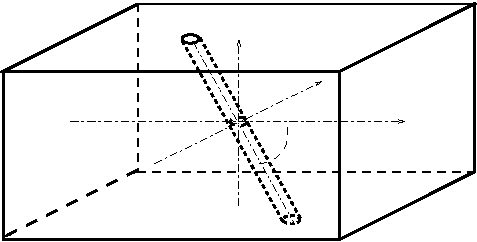
\includegraphics[scale=0.75]{./well1.png}
      \caption{The circular slanted well. \label{meshsucces}}
    \end{center}
  \end{figure}
  The permeability tensor $\Lambda$ is constant and anisotropic in the third coordinate direction:
  $$
  \Lambda =\begin{pmatrix} ~1~&~0~&~0~\\0& 1&0\\0&0& \tau\end{pmatrix},
  $$
with $\tau = 0.2$.
The solution $\bu$, inspired from \cite{aav-03-well}, is equal to $0$ on the well boundary $\dr W\cap \dr\O$ and is strictly positive inside $\O$. 
It is defined by $\bar u(x,y,z) $ $=$ $v(Y(x,y,z),$ $ Z(x,y,z))$, where the linear functions $Y$ and $Z$ are defined by 
\[
 Y(x,y,z) =  y \hbox{ and } Z(x,y,z) = (\sin \beta) x + \frac{\cos \beta}  {\sqrt{\tau}} z,
\]
with $\beta = \arctan( \frac {\tan \theta}{\sqrt{\tau}})$.
We then define $\alpha = \sqrt{(\frac {\sin \beta} {\sin \theta})^2 - 1}$, and we let $a = \alpha r_w$ and $\mu_0 = \log\left(\frac {1} \alpha + \sqrt{\frac {1} {\alpha^2} + 1}\right) $.
The function $v$ is given by 
\[
v(Y,Z) =  \log (\sqrt{S} + \sqrt{S +1} ) - \mu_0,\]
with  $S> 0$  such that $a^2  S^2 + (a^2 - Y^2 -Z^2)  S  -Y^2 = 0$.


\medskip


The simulation uses 3D meshes ({\tt{mesh}1} -- {\tt{mesh}7}) created for the 3D benchmark of \cite{3Dbench}. These meshes are refined around the well as can be seen in Figure \ref{fig:wellmesh}. The first step of the meshing process is to create a radial mesh that is exponentially refined down to the well boundary. This radial local refinement implies a matching mesh between the radial grid and the reservoir Corner Point Geometry grid using hexahedral cells.

\begin{figure}[ht]
\centering{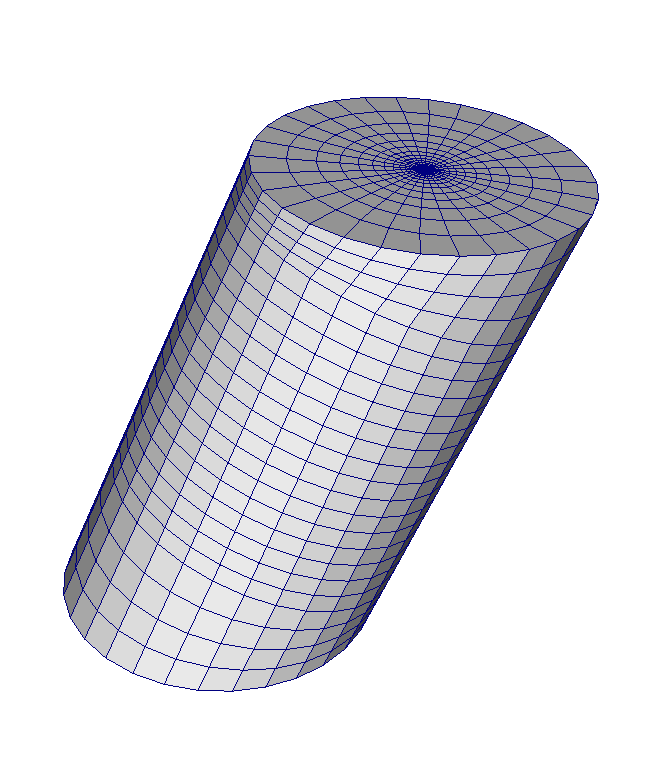
\includegraphics[scale=.12]{figNum/radial3D.png}
\hspace*{10mm}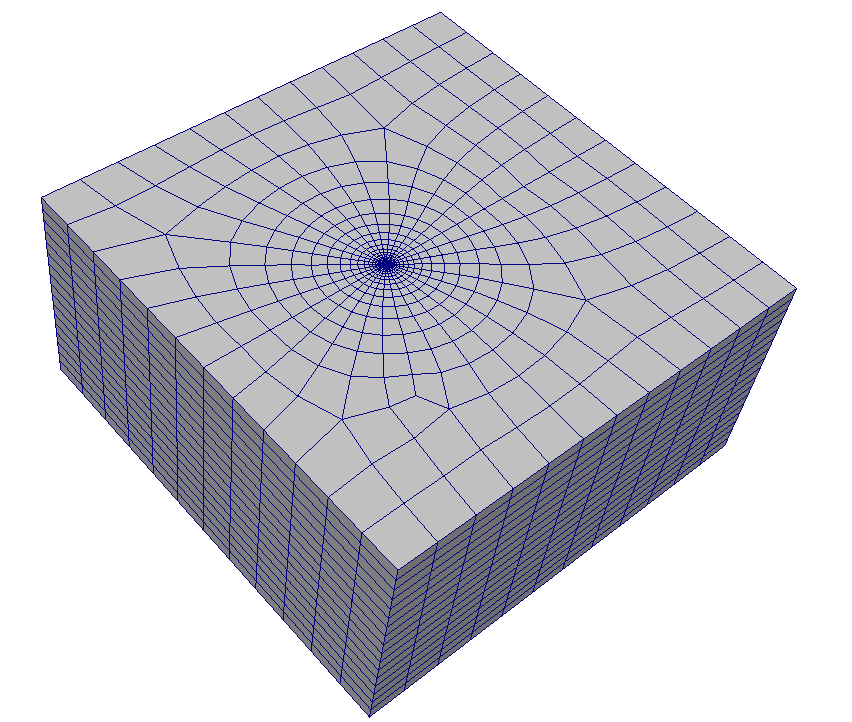
\includegraphics[scale=.12]{figNum/rac_quad.png}}
\caption{Radial mesh without (left) and with transition zone (right).\label{fig:wellmesh}
}
\end{figure}

  
 We present in Table \ref{tab:3Dslantedwell} the results obtained on these grids using on one hand the SUSHI scheme presented in Chapter \ref{chap:hmm} (see Remark \ref{rem:lksushi} for the particular choice of the discrete gradient), and on the other hand the VAG scheme\index{vertex approximate gradient (VAG)} presented in Chapter \ref{chap:Galerkin}, Section \ref{sec:vag}. 
 The orders  of convergence are computed with respect to the number of unknowns at the power $1/3$, which cannot put in evidence the effects of local refinement. The main observation is that these two gradient discretisations are adapted to complex polytopal meshes issued from a quite realistic situation (see Figure \ref{fig:sliceswellmesh} for a visualisation of the approximate solution).
 

\begin{table}
\begin{center}
\begin{tabular}{|c||c|c||c|c|}
\hline
&\multicolumn{2}{c||}{SUSHI}&\multicolumn{2}{c|}{VAG}\\
\hline
&$u$&$\nabla u$&$u$&$\nabla u$\\
\hline
 \tt{mesh}1 &  3.79E-03  &  9.69E-02   &  6.22E-03  &  5.73E-02 \\
 order &  0.69 &   2.03 &   3.24  &  3.03 \\
 \tt{mesh}2 &  3.07E-03  &  5.21E-02 &  2.60E-03 &   2.53E-02  \\
 order &  2.42 &   2.29 &  3.46 &   2.88E+00 \\
 \tt{mesh}3 &  1.60E-03 &  2.81E-02 &   1.10E-03 &  1.24E-02\\
 order &  1.38 &    1.08 &   1.72 &   1.69 \\
 \tt{mesh}4 &  1.10E-03 &  2.10E-02 &   7.13E-04 &   8.10E-03 \\
 order &  1.45 &   1.19 &   2.64 & 1.05 \\
 \tt{mesh}5 &  7.77E-04 &   1.57E-02 &   3.85E-04 &   6.35E-03  \\
 order &  2.39 &    1.89 &   3.60 &  1.46 \\
 \tt{mesh}6 &  4.78E-04 &   1.07E-02 &   1.90E-04 &  4.77E-03  \\
 order &   0.26 &    0.37&   -0.16 &  -0.06  \\
 \tt{mesh}7 &  4.56E-04 &   9.98E-03 &   1.95E-04 &  4.82E-03   \\
\hline
\end{tabular}
\caption{$L^2$ error for the solution and its gradient in the case of the 3D slanted well, using schemes SUSHI and VAG. ``Order'' represents the rate of
convergence from the line above to the line below.}\label{tab:3Dslantedwell}
\end{center}
\end{table}
  
  
  
\begin{figure}[ht]
%\resizebox{\textwidth}{!}{
%\includegraphics[scale=.12]{figNum/coupe806_1.pdf}
%\includegraphics[scale=.12]{figNum/coupe806_2.pdf}
%\includegraphics[scale=.12]{figNum/coupe806_3.pdf}
%}
\begin{center}
\begin{tabular}{cc}
\includegraphics[scale=.025]{figNum/coupe806_1.pdf} & \raisebox{6.8em}{\multirow{2}{*}{\includegraphics[scale=.025]{figNum/coupe806_3.pdf}}}\\
\includegraphics[scale=.025]{figNum/coupe806_2.pdf}
\end{tabular}
\end{center}
%\caption{Approximate solution using SUSHI on {\tt mesh}3, from left to right: slices in planes $x = .2$, $y = .2$ and $z= .4$.  \label{fig:sliceswellmesh} }
\caption{Approximate solution using SUSHI on {\tt mesh}3. Top left: slice in the plane $x = 0.2$;
bottom left: slice in the plane $y = 0.2$; right: slice in the plane $z= 0.4$.  \label{fig:sliceswellmesh} }
\end{figure}

\section{ADGGD for the $p-$Laplace problem}\label{sec:numplap}
\index{plapl@$p$-Laplace problem}
We consider the $p$-Laplace problem \eqref{eq:plap1} with Dirichlet boundary conditions \eqref{chapplap:bc-dir-hom}.
The aim of this section is to assess the accuracy of the error estimate provided by Theorem \ref{thm:convgradschplap}. 

\subsection{The one-dimensional case}\label{sec:numplapdimone}

We consider the case where $d=1$, $\Omega = (0,1)$ and $f(x) = 1$. The analytical solution is then given by
\be\label{num.test:plap.analytic}
 \bu(x) = \frac {p-1} p \left[ \left(\frac 1 2\right)^{p/(p-1)} - \left|x - \frac 1 2\right|^{p/(p-1)}\right].
\ee


We consider a mesh with constant space step $h = 1/N$ (with $N\in \N^\star$) and we use Scheme \eqref{gradsch_plap} together with the Discontinuous Galerkin gradient discretisation given by Definition \ref{chapdg:def:dggd},
with $k=1$ and $\beta = 1/2$ (note that in the one-dimensional case, the two definitions \eqref{chapdg:eq:defgraddisc} and \eqref{chapdg:eq:defgraddisca} for the discrete gradient are identical, so the DGGD is identical to the ADGGD).

\begin{figure}[!ht]
  \centering
 \subfigure[$p = 1.5$]{\label{fig:punpcinq}
 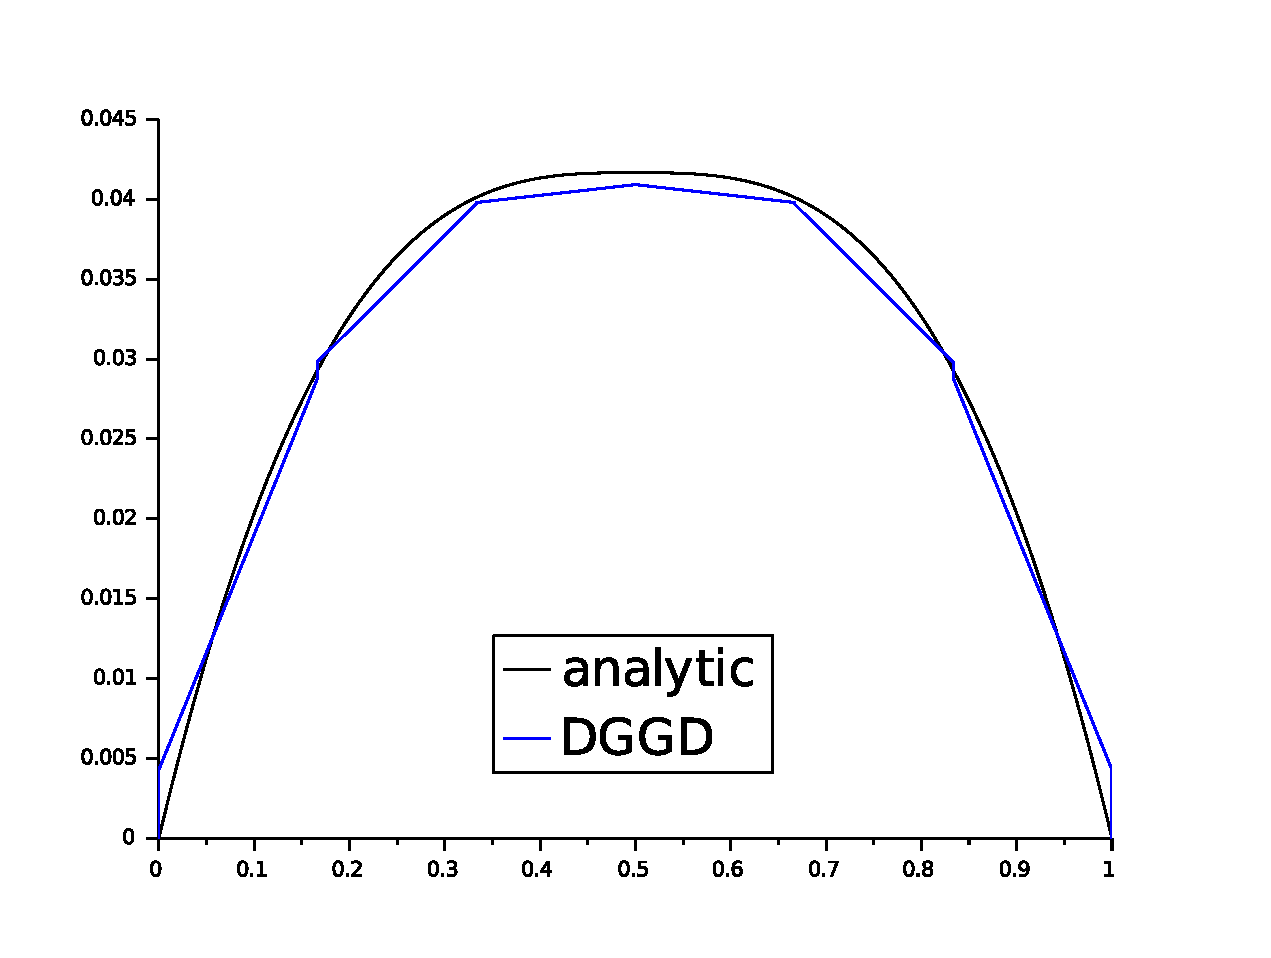
\includegraphics[scale=0.25]{figNum/casep1p5.pdf}}
 \subfigure[$p = 2$]{\label{fig:pdeux}
 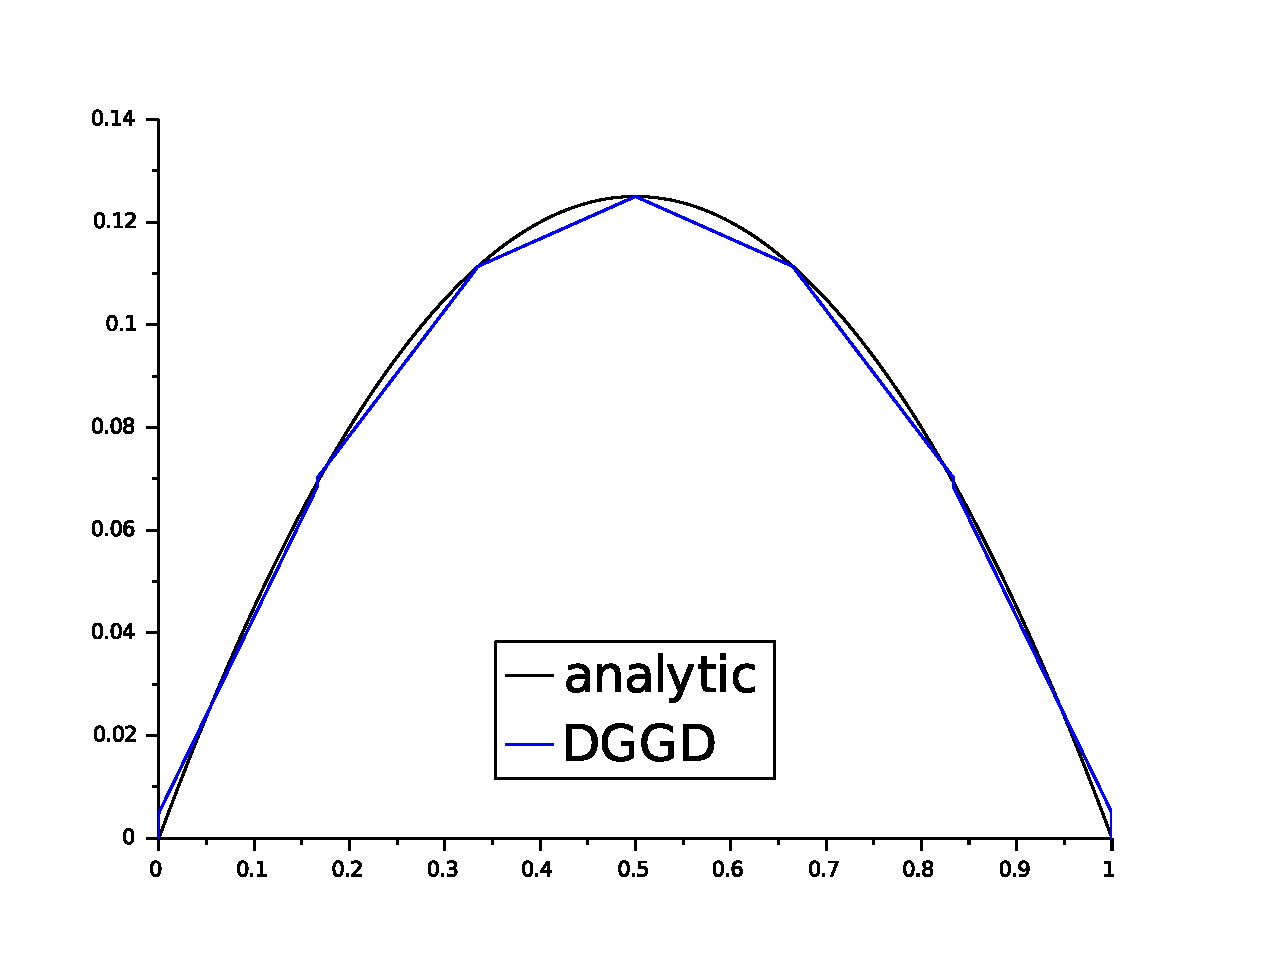
\includegraphics[scale=0.25]{figNum/casep2.pdf}}
 \subfigure[$p = 4$]{\label{fig:pquatre}
 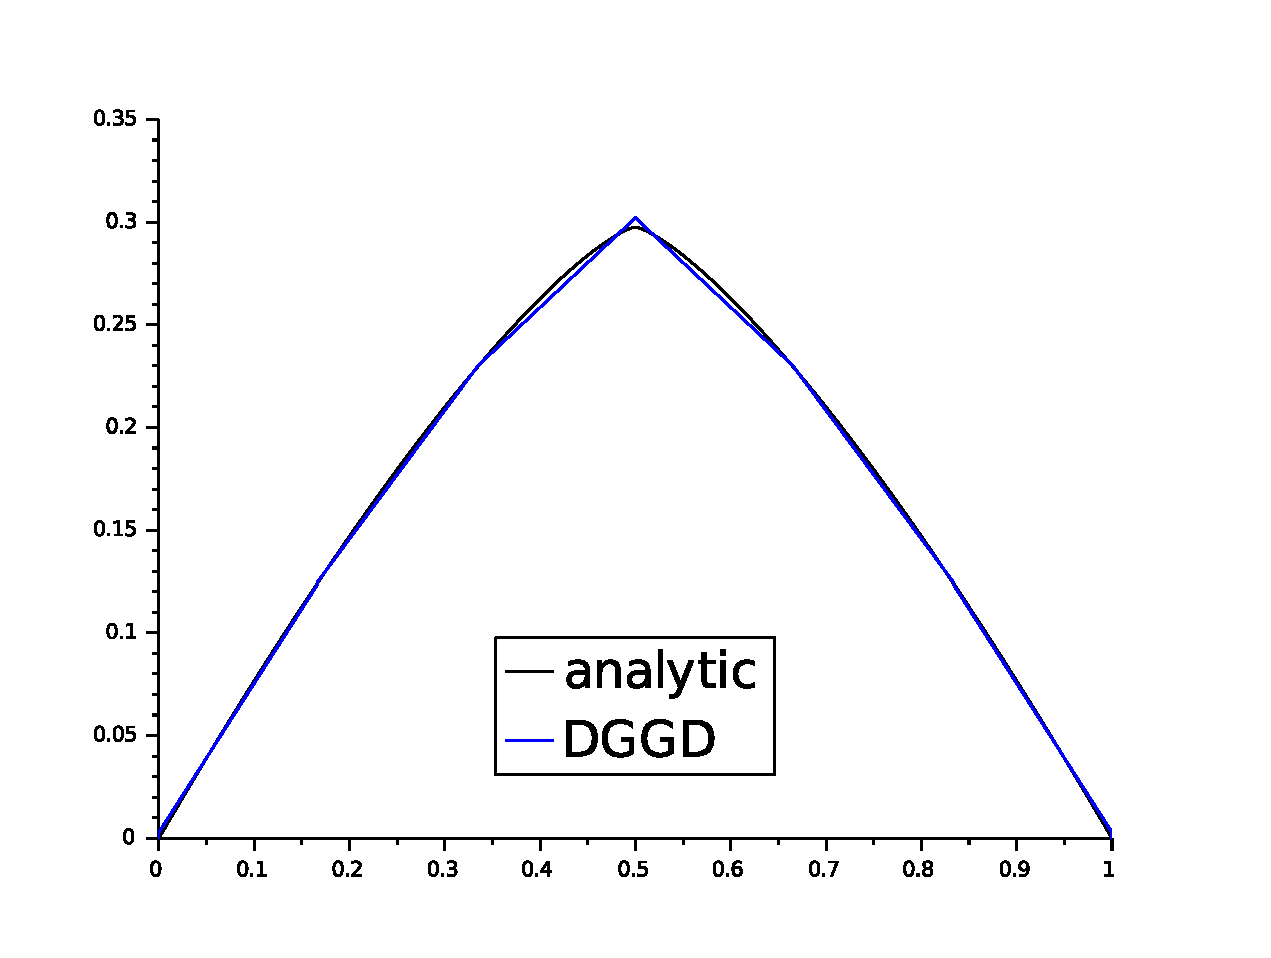
\includegraphics[scale=0.25]{figNum/casep4.pdf}}
\caption{Exact and DGGD approximate solutions for the $p$-Laplace equation ($k=1$, $\beta = 0.5$, $N=6$).
\label{fig:plap}}
\end{figure}

We see in Figure \ref{fig:plap} that the approximate solution matches quite well the analytical solution for $N=6$, considering the three cases $p=1.5$, $p=2$ and $p=4$.

\begin{table}
\begin{center}
\begin{tabular}{|c|c|c||c|c||c|c|}
\hline
&\multicolumn{2}{c||}{$p=1.5$}&\multicolumn{2}{c||}{$p=2$}&\multicolumn{2}{c|}{$p=4$}\\
\hline
&$u$&$\nabla u$&$u$&$\nabla u$&$u$&$\nabla u$\\
\hline
$N=10$&5.51E-04&6.34E-03&9.65E-04&9.40E-03&1.48E-03&8.11E-03\\
\hline
order & 1.85 & 1.55 & 1.96 & 1.50 & 1.62  & 1.33\\
\hline
$N=20$ & 1.53E-04 & 2.17E-03 & 2.48E-04 & 3.32E-03 & 4.80E-04 & 3.23E-03\\
\hline
order & 1.92 & 1.61 & 1.98 & 1.50 & 1.60 & 1.29\\
\hline
$N=40$ & 4.02E-05 & 7.11E-04 & 6.29E-05 & 1.18E-03 & 1.58E-04 & 1.33E-03 \\
\hline
order & 1.96 & 1.64 & 1.99 & 1.50 & 1.59 & 1.59\\
\hline
$N=80$ & 1.03E-05 & 2.28E-04 & 1.58E-05 & 4.15E-04 & 5.24E-05 & 5.51E-04\\
\hline
order & 1.98 & 1.65 & 2.00 & 1.50 & 1.59 & 1.26\\
\hline
$N=160$ & 2.62E-06 & 7.26E-05 & 3.97E-06 & 3.97E-06 & 1.74E-05 & 2.30E-04\\
\hline
\end{tabular}
\caption{Errors and rates of convergences, on the functions and the gradient, for the ADGGD
GS applied to the $p$-Laplace equation in dimension 1. ``Order'' represents the rate of
convergence from the line above to the line below.}\label{tab:plaponed}
\end{center}
\end{table}


Combining Remark \ref{rem:basicratesp} and Lemmas \ref{chapdg:lem:gdconsistency}
and \ref{lem:dg:highorderwd} (for $\ell=k=1$) shows that, if the solution is smooth enough,
the expected rates of convergence in $L^p$ norms on both the function and gradient
are $\mathcal O(h^{p-1})$ if $p\le 2$ and $\mathcal O(h^{1/(p-1)})$ if $p\ge 2$.
Hence, for $p=1.5$ (resp. 2, resp. 4), the expected order would be $\mathcal O(h^{0.5})$
(resp. $\mathcal O(h)$, resp. $\mathcal O(h^{1/3})$).
As seen in Table \ref{tab:plaponed}, these orders are pessimistic as, even for the 
non-smooth function given by \eqref{num.test:plap.analytic}, the theoretical rates
are beat by at least half an order. This was expected for the $L^p$ norm of the
function, as estimates that are common to the function and the gradient,
as in Theorem \ref{thm:convgradschplap}, are known to be sub-optimal for the function
(but, at least for linear problems, better estimates can be established in the GDM
framework \cite{DN16}). This was less obvious for the gradient.


\subsection{The two-dimensional case}\label{sec:numplapdimtwo}

We take here $d=2$, $\Omega = (0,1)\times(0,1)$ and $f(\x) = 2$ for all $\x\in\O$. 
Set $\x_\O=(1/2,1/2)$ and fix non-homogeneous Dirichlet boundary conditions in agreement with the analytical solution
\be\label{num.test:plap.analytictwod}
 \bu(\x) = \frac {p-1} p \left[ \left(\frac 1 {\sqrt{2}}\right)^{p/(p-1)} - \left|\x - \x_\O\right|^{p/(p-1)}\right].
\ee
We apply the GS \eqref{gradsch_plap} together with the Average Discontinuous Galerkin Gradient Discretisation given by Definition \ref{chapdg:def:dggd} and definition \eqref{chapdg:eq:defgraddisca} for the discrete gradient, letting $k=1$ and $\beta = 4/5$. Note that the discrete gradient is piecewise constant, which leads to simple computations, in particular for the $p-$Laplace problem. The triangular meshes from the family \texttt{mesh1} of \cite{2Dbench} are used for the numerical tests.

\begin{figure}[!ht]
  \centering
 \subfigure[\texttt{mesh1\_1}]{\label{fig:mesh1}
 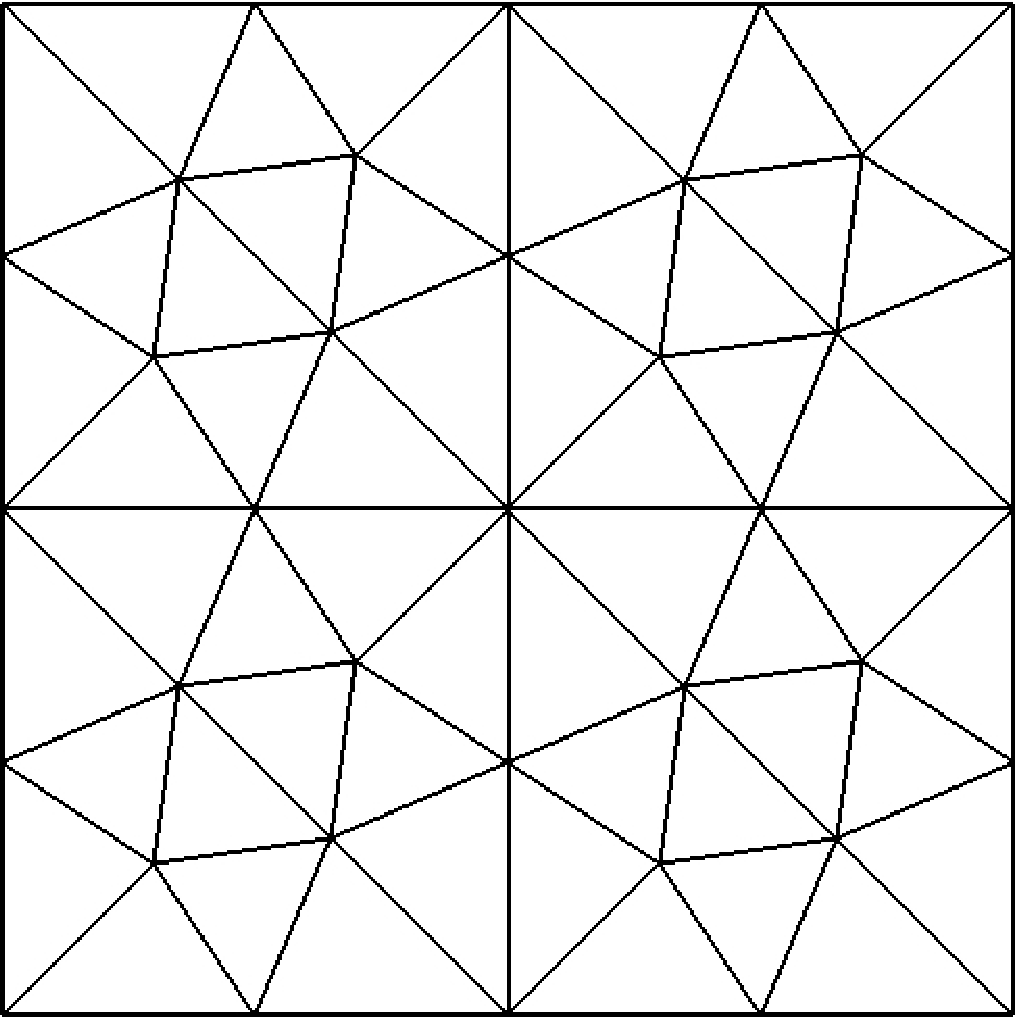
\includegraphics[scale=0.2]{figNum/mesh1.pdf}}
 \subfigure[$p = 1.5$]{\label{fig:punpcinq2d}
 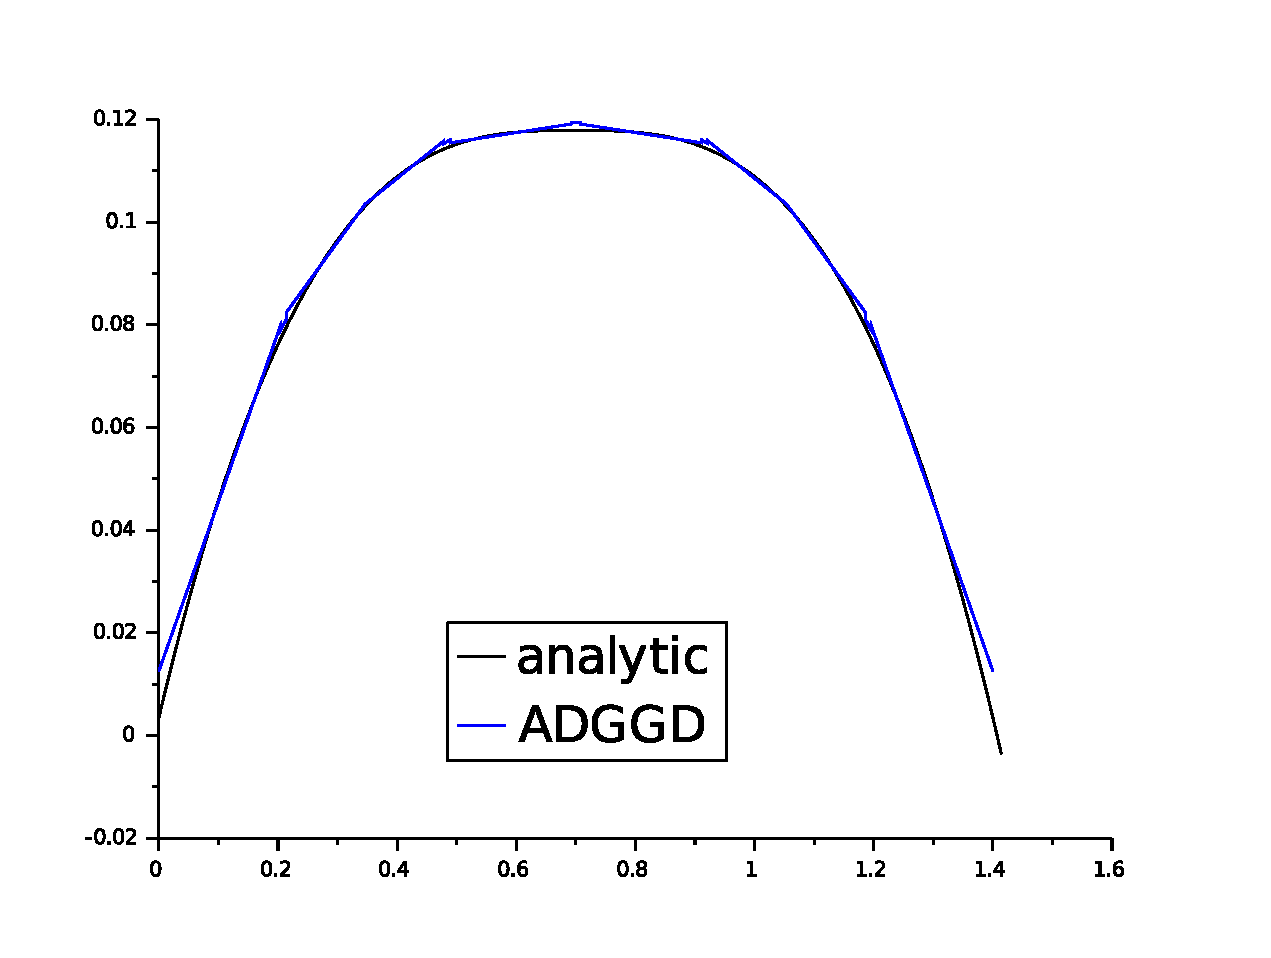
\includegraphics[scale=0.25]{figNum/profilp1p5.pdf}}
 \subfigure[$p = 2$]{\label{fig:pdeux2d}
 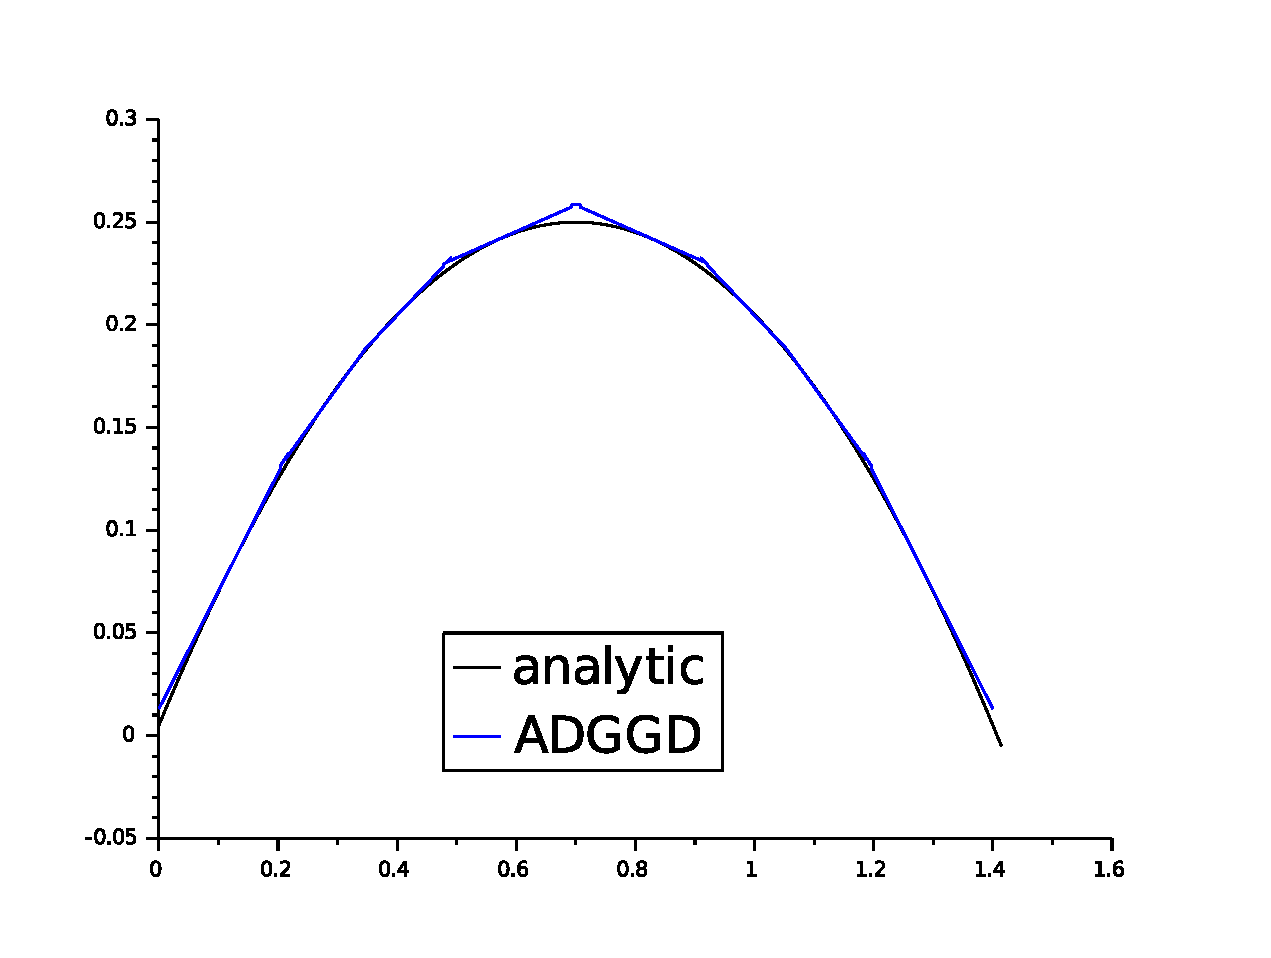
\includegraphics[scale=0.25]{figNum/profilp2.pdf}}
 \subfigure[$p = 4$]{\label{fig:pquatre2d}
 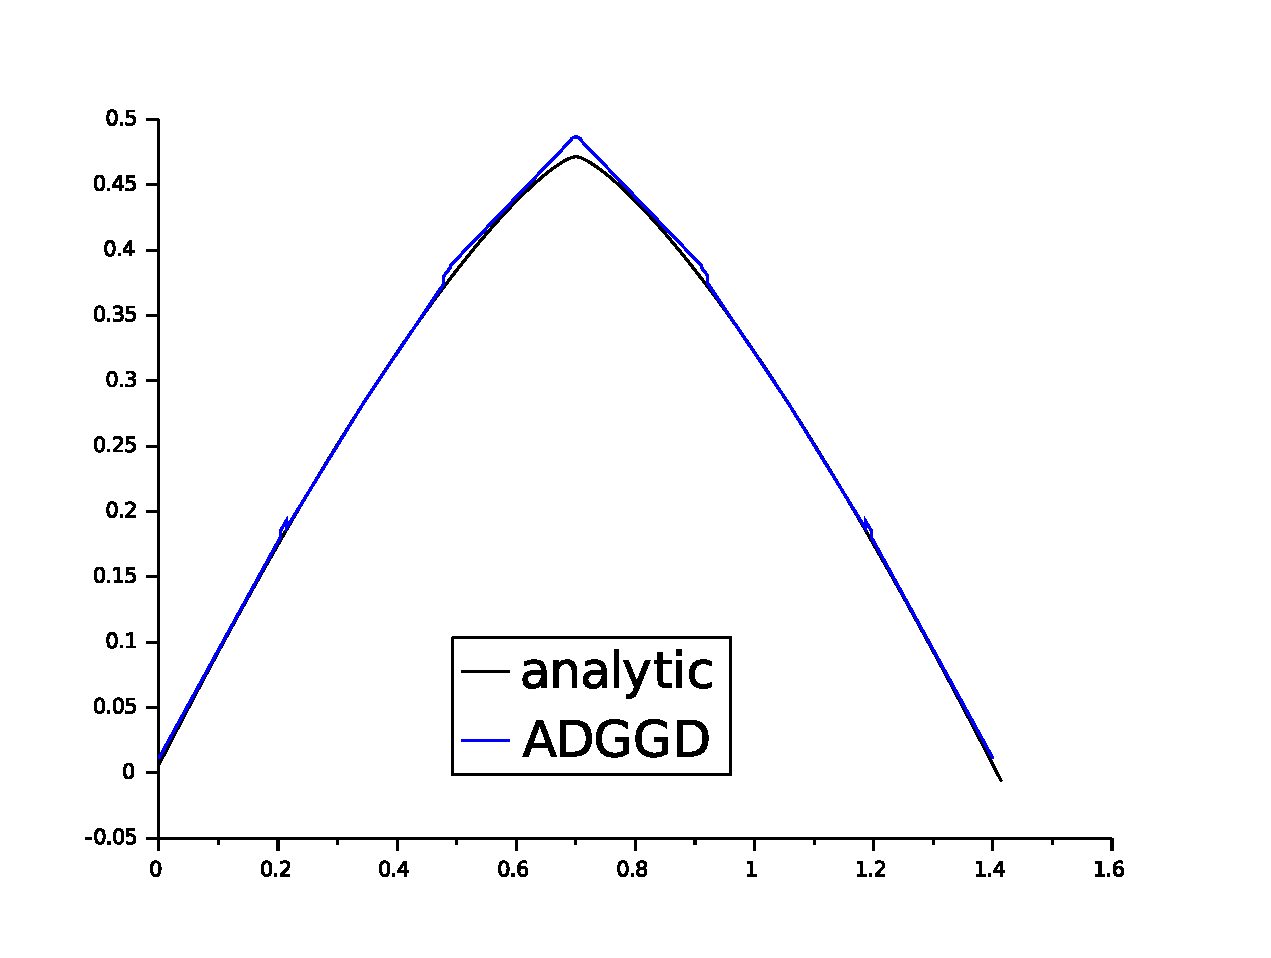
\includegraphics[scale=0.25]{figNum/profilp4.pdf}}
\caption{Mesh \texttt{mesh1\_1} and exact and ADGGD approximate profiles along the line $x_2 = x_1 + 0.01$ for the $p$-Laplace equation ($k=1$, $\beta = 0.8$, using \texttt{mesh1\_1}).
\label{fig:plap2d}}
\end{figure}

Figure \ref{fig:plap2d} presents the profile of the approximate solution along the line $x_2 = x_1 + 0.01$,
for the three cases $p=1.5$, $p=2$ and $p=4$, on the coarsest triangular mesh.
We notice a rather good match of approximate solution on this line.

Table \ref{tab:plaptwod} shows that the practical rates of convergence are better
than the theoretical ones from Theorem \ref{thm:convgradschplap}; however, the
rates for the gradient
are degraded with respect to the similar test case in dimension $d=1$.

\begin{table}
\begin{center}
\begin{tabular}{|c|c|c||c|c||c|c|}
\hline
&\multicolumn{2}{c||}{$p=1.5$}&\multicolumn{2}{c||}{$p=2$}&\multicolumn{2}{c|}{$p=4$}\\
\hline
&$u$&$\nabla u$&$u$&$\nabla u$&$u$&$\nabla u$\\
\hline
\texttt{mesh1\_1}&  0.944E-03 &  0.314E-02&  0.120E-02 &  0.423E-02 &  0.138E-02 &  0.432E-02\\
\hline
order &   1.96 &   1.48&   1.95 &   1.42&   1.32 &   1.41\\
\hline
\texttt{mesh1\_2} &  0.243E-03 &  0.113E-02&  0.308E-03 &  0.158E-02 &  0.555E-03 &  0.162E-02\\
\hline
order &   1.97 &   1.48&   1.98 &   1.38 &   1.57 &   1.16\\
\hline
\texttt{mesh1\_3} &  0.621E-04 &  0.405E-03 &  0.783E-04 &  0.608E-03&  0.187E-03 &  0.727E-03\\
\hline
order &   1.98 &   1.40&   1.99 &   1.31&   1.67 &   0.93\\
\hline
\texttt{mesh1\_4}&  0.157E-04 &  0.154E-03 &  0.197E-04 &  0.245E-03&  0.587E-04 &  0.381E-03\\
\hline
order&   1.99 &   1.29 &   1.99 &   1.23&   1.73 &   0.85 \\
\hline
\texttt{mesh1\_5}&  0.396E-05 &  0.630E-04  &  0.495E-05 &  0.105E-03&  0.177E-04 &  0.211E-03\\
\hline
\end{tabular}
\caption{Errors and rates of convergences, on the functions and the gradient, for the ADGGD
GS applied to the $p$-Laplace equation in dimension 2. ``Order'' represents the rate of
convergence from the line above to the line below.}\label{tab:plaptwod}
\end{center}
\end{table}


      


\section{An example of the application of the GDM to a degenerate parabolic problem}\label{secexampletransient}

We consider the evolution problem \eqref{chpdeg:pbintrot} in 2D, letting $\beta(s) = s$ and $\Lambda = {\rm I}_d $, which means that we approximate the Stefan problem\index{Stefan problem}. The scheme used here is the VAG scheme
described in Section \ref{sec:vag}. The domain is
$\Omega=(0,1)^2$, and we use the following definition of $\zeta (\bu)$,
$$
 \zeta (\bu) =
\left\{\begin{array}{ll}  
\bu & \mbox{ if } \bu<0,\\
\bu-1 & \mbox{ if } \bu>1,\\
0 & \mbox{ otherwise}.
\end{array}\right.
$$ 
Dirichlet boundary conditions are given by $\bu=-1$ on $\partial \Omega$ and the initial condition is $\bu(\x,0) = 2$. Four grids are used for the computations: a Cartesian grid with $32^2 = 1024$ cells, the same grid randomly perturbed, a triangular grids with $896$ cells, and a ``Kershaw mesh'' with $1089$ cells as illustrated in Figure \ref{fig:2D_T25} (such meshes are standard in the framework of underground engineering). The final time is $0.1$ and the simulation is ran with a constant time step of $0.001$.

Figures \ref{fig:2D_T25}, \ref{fig:2D_T50}, \ref{fig:2D_T75} and \ref{fig:2D_T100} represent the discrete solution $u(\cdot,t)$ on all grids for $t= 0.025, 0.05, 0.075$ and $0.1$. For a better comparison we have also plotted the interpolation of $u$ along two lines of the mesh. The first line is horizontal and joins the two points $(0,0.5)$ and $(1,0.5$). The second line is diagonal and joins points $(0,0)$ and $(1,1)$. The results 
for these slices are shown in Figures
\ref{fig:filtre_x} and \ref{fig:filtre_d}.

The numerical outputs are weakly dependent on the grid, and the interface between the regions $u<0$ and $u>1$ are located at the same place for all grids. It is worth noticing that this remains true even for the very irregular Kershaw mesh
(which presents high regularity factors $\theta_\polyd$ -- see \eqref{def:reg.theta},
that is high ratios for some cells between the radii of inscribed balls and the diameter of the cell).

\begin{figure}[ht]
  \centering
 \subfigure[$t=0.025$]{\label{filtre_x_T25}
 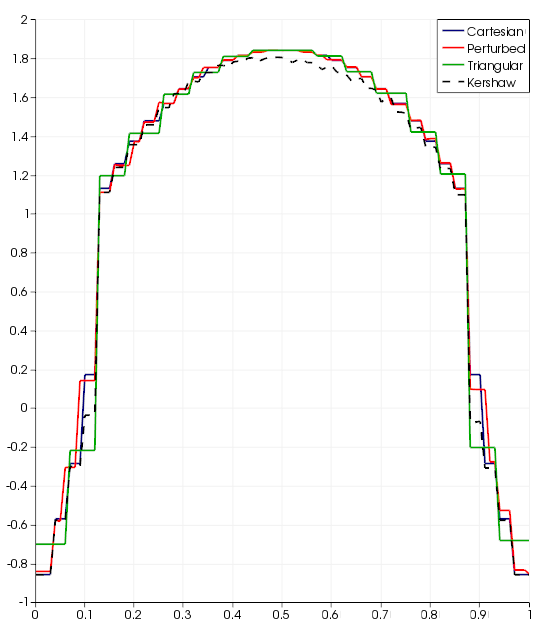
\includegraphics[scale=0.19]{figNum/filtre_x_T25.png}}
  \subfigure[$t=0.050$]{\label{filtre_x_T50}
 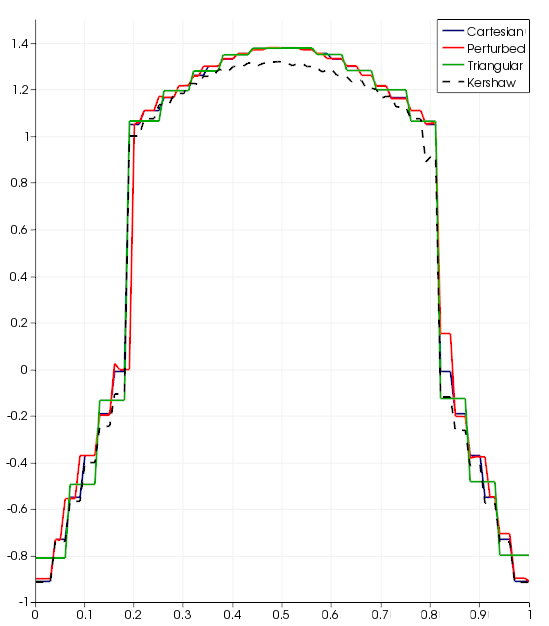
\includegraphics[scale=0.19]{figNum/filtre_x_T50.png}}\\
   \subfigure[$t=0.075$]{\label{filtre_x_T75}
 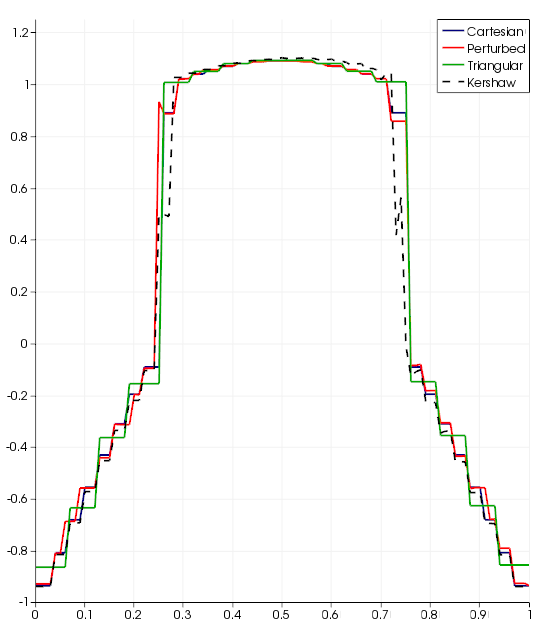
\includegraphics[scale=0.19]{figNum/filtre_x_T75.png}}
    \subfigure[$t=0.1$]{\label{filtre_x_T100}
 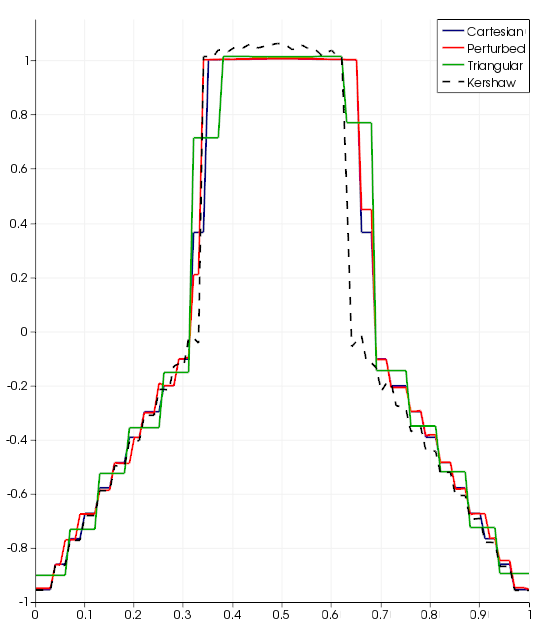
\includegraphics[scale=0.19]{figNum/filtre_x_T100.png}}
  \caption{Interpolation of $u$ along the line $x_2=0.5$ of the mesh for each grids: Cartesian in blue, perturbed Cartesian in red, triangular in green, and Kershaw in black dashed.  \label{fig:filtre_x}}
\end{figure}


\begin{figure}[ht]
  \centering
 \subfigure[$t=0.025$]{\label{filtre_d_T25}
 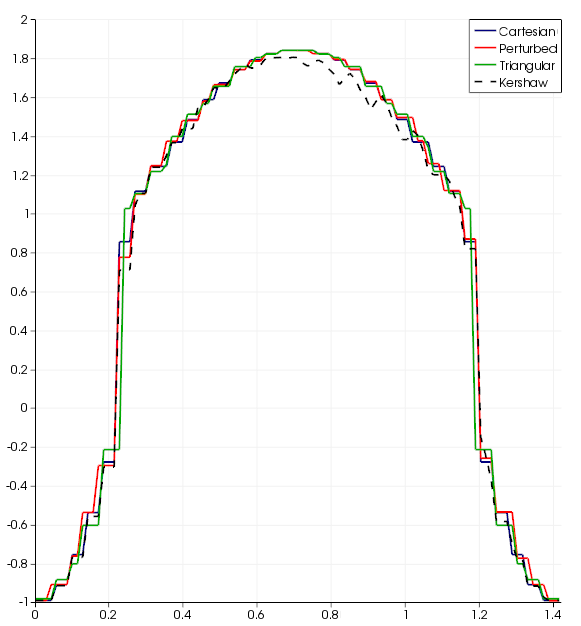
\includegraphics[scale=0.185]{figNum/filtre_diag_T25.png}}
  \subfigure[$t=0.050$]{\label{filtre_d_T50}
 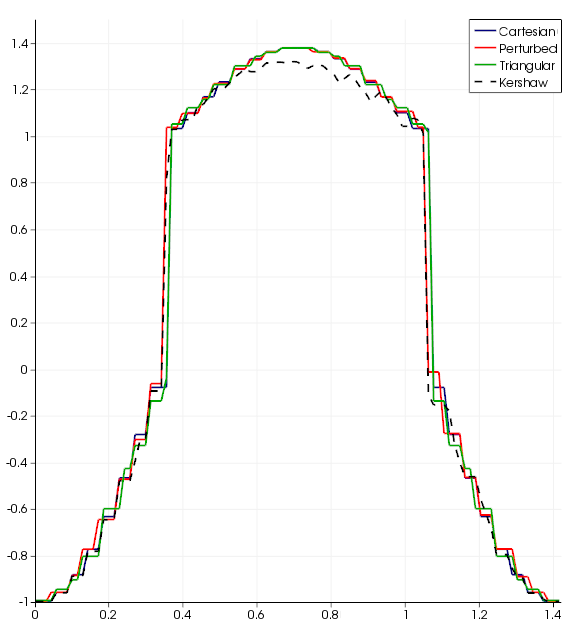
\includegraphics[scale=0.185]{figNum/filtre_diag_T50.png}}\\
   \subfigure[$t=0.075$]{\label{filtre_d_T75}
 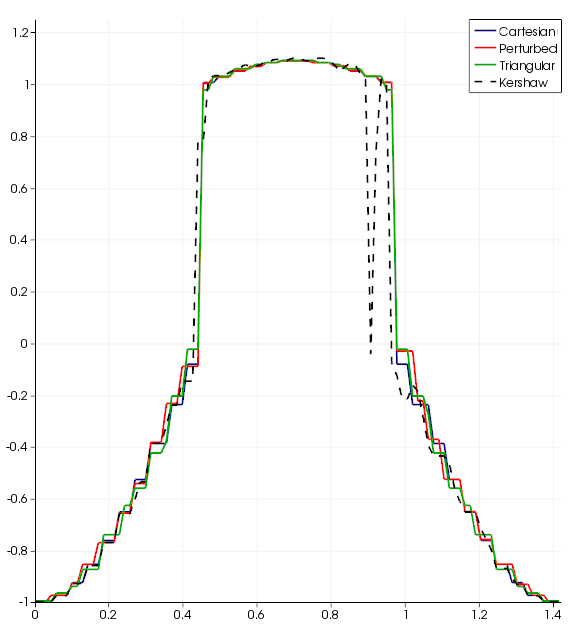
\includegraphics[scale=0.185]{figNum/filtre_diag_T75.png}}
    \subfigure[$t=0.1$]{\label{filtre_d_T100}
 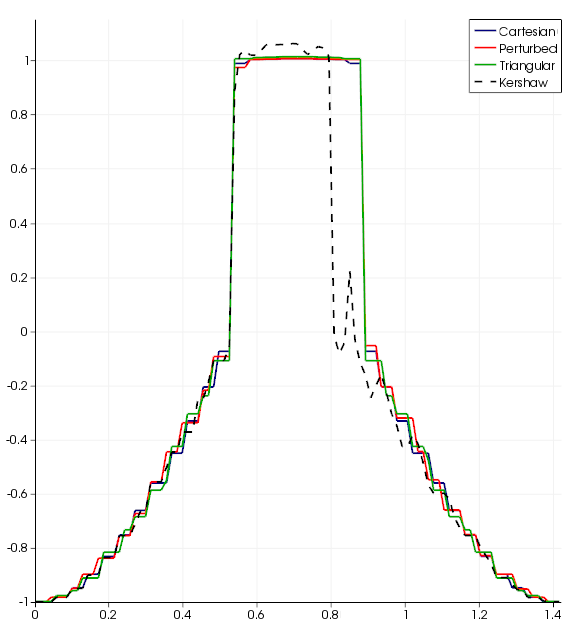
\includegraphics[scale=0.185]{figNum/filtre_diag_T100.png}}
  \caption{Interpolation of $u$ along a diagonal axe of the mesh for each grids: Cartesian in blue, perturbed 
Cartesian in red, triangular in green, and Kershaw in black dashed.  \label{fig:filtre_d}
}
\end{figure}


\begin{figure}[ht]
%trim=left bottom right top
 \centering
  \subfigure[Cartesian]{\label{2D_T25_cart}
  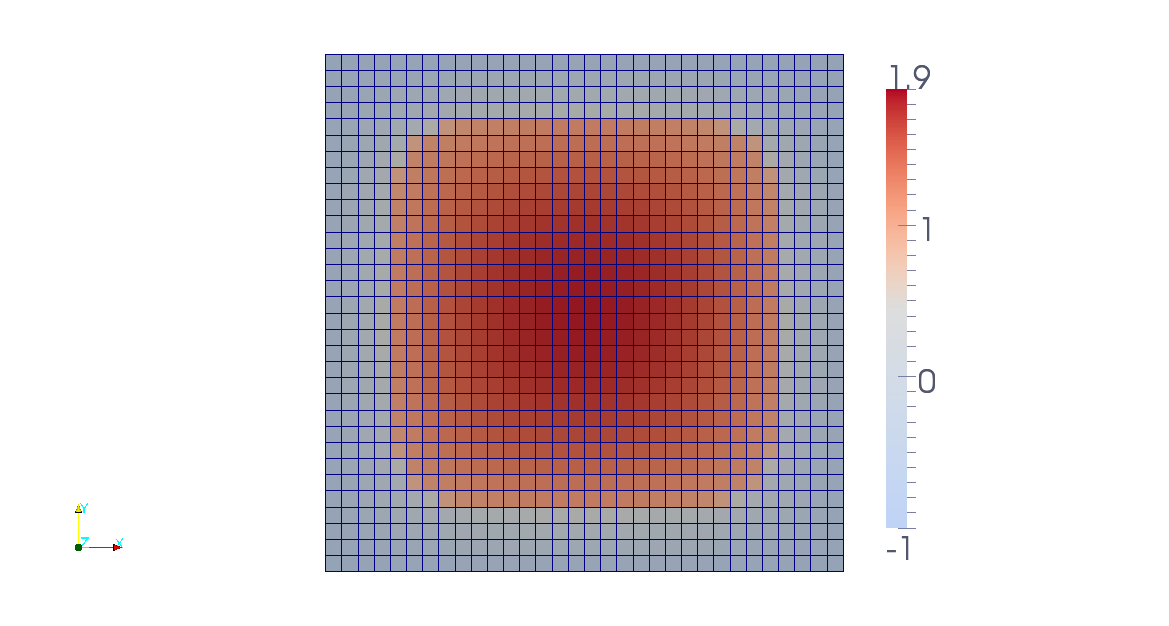
\includegraphics[trim=11.cm 2.cm 11.cm 2.cm,clip=true,scale=0.18]{figNum/cart_T25.png}}
  \subfigure[Perturbed Cartesian]{\label{2D_T25_rand}
  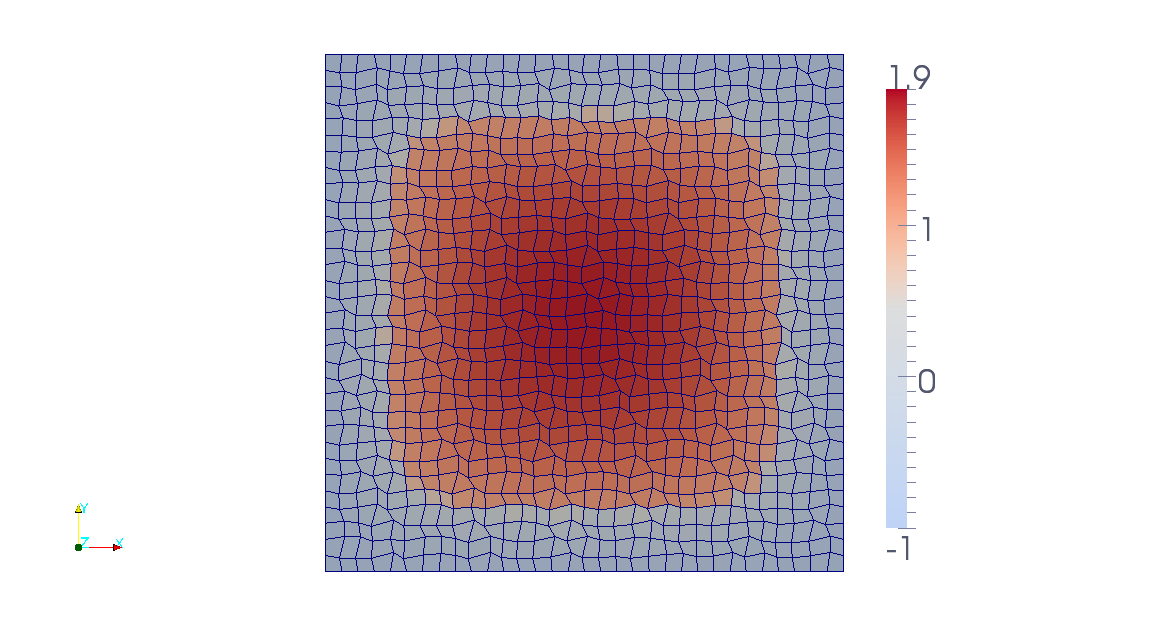
\includegraphics[trim=11.cm 2.cm 11.cm 2.cm,clip=true,scale=0.18]{figNum/rand_T25.png}}\\
  \subfigure[Triangular]{\label{f2D_T25_tria}
  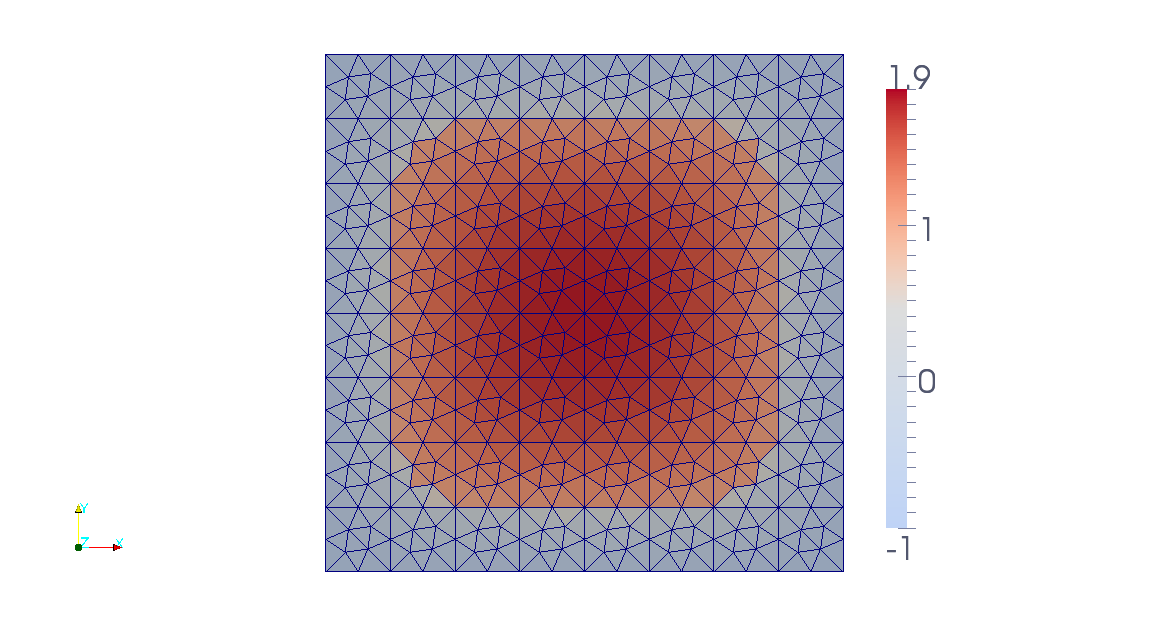
\includegraphics[trim=11.cm 2.cm 11.cm 2.cm,clip=true,scale=0.18]{figNum/tri_T25.png}}
  \subfigure[Kershaw]{\label{2D_T25_ker}
  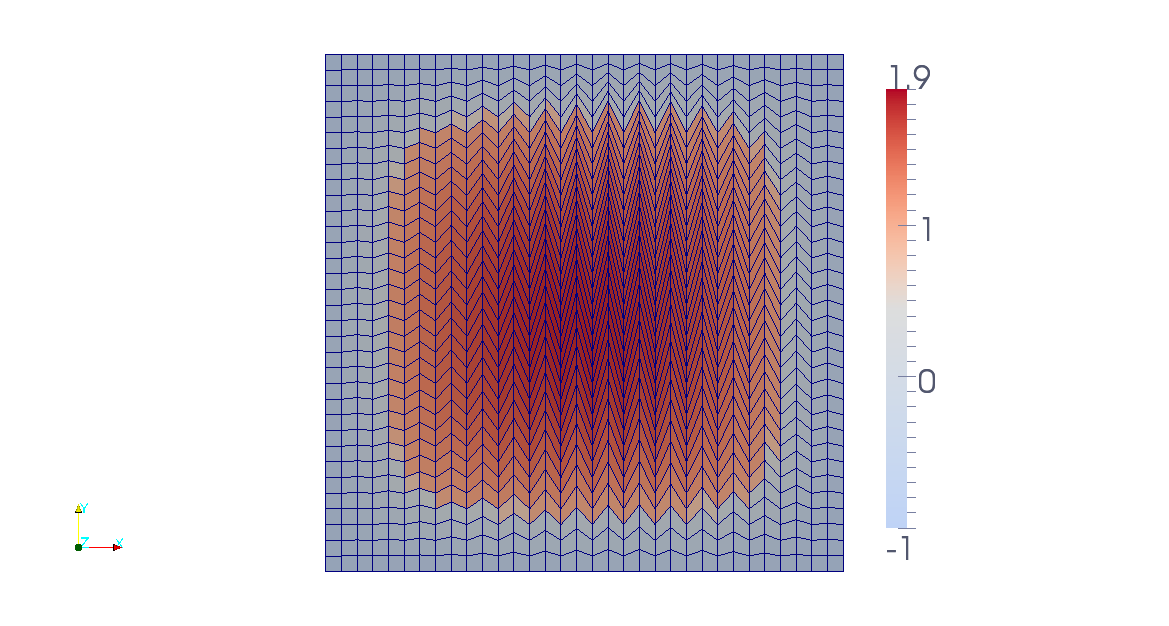
\includegraphics[trim=11.cm 2.cm. 7.cm 2.cm,clip=true,scale=0.18]{figNum/ker_T25.png}}
\caption{Discrete solution $u$ on all grids at $t=0.025$.\label{fig:2D_T25}
}
\end{figure}

\begin{figure}[ht]
%trim=left bottom right top
 \centering
  \subfigure[Cartesian]{\label{2D_T50_cart}
  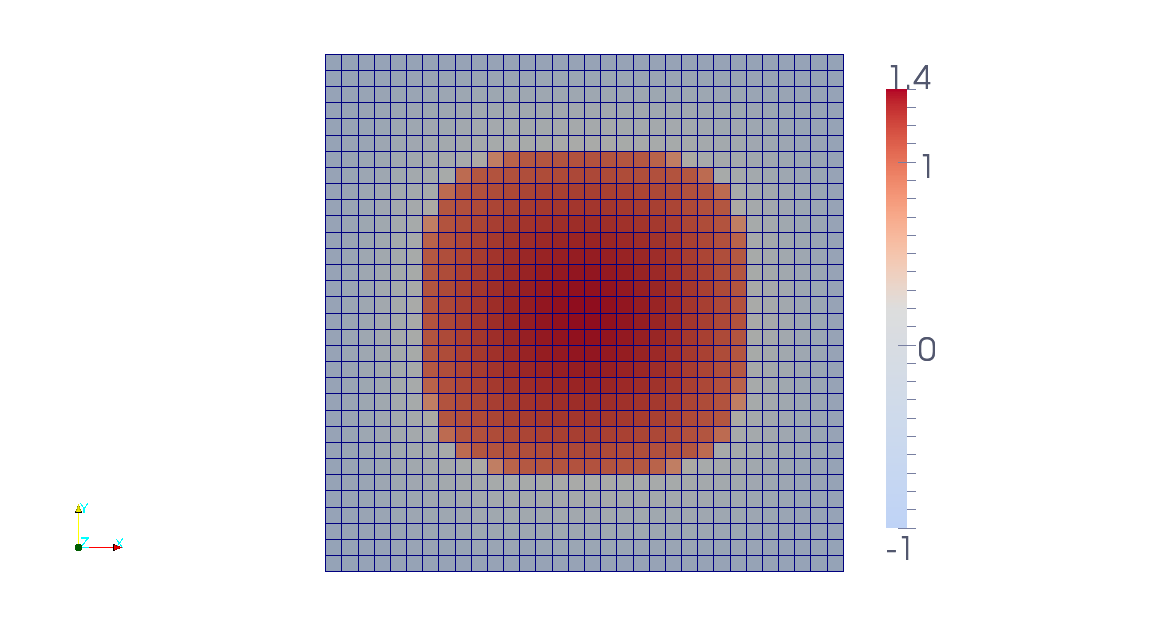
\includegraphics[trim=11.cm 2.cm 11.cm 2.cm,clip=true,scale=0.18]{figNum/cart_T50.png}}
  \subfigure[Perturbed Cartesian]{\label{2D_T50_rand}
  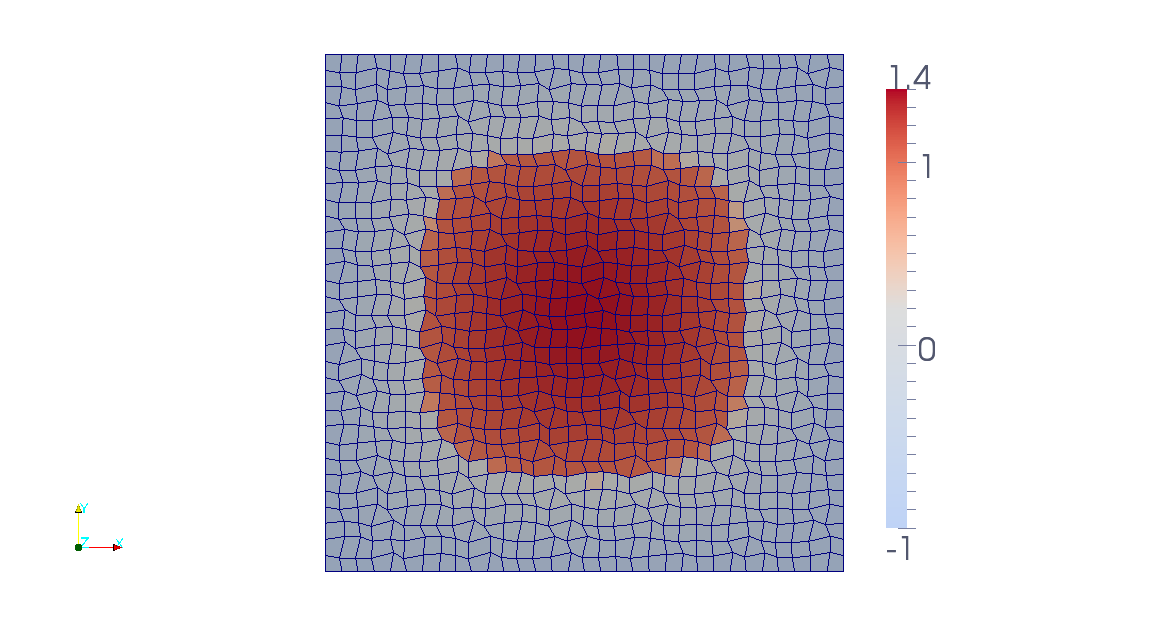
\includegraphics[trim=11.cm 2.cm 11.cm 2.cm,clip=true,scale=0.18]{figNum/rand_T50.png}}\\
  \subfigure[Triangular]{\label{f2D_T50_tria}
  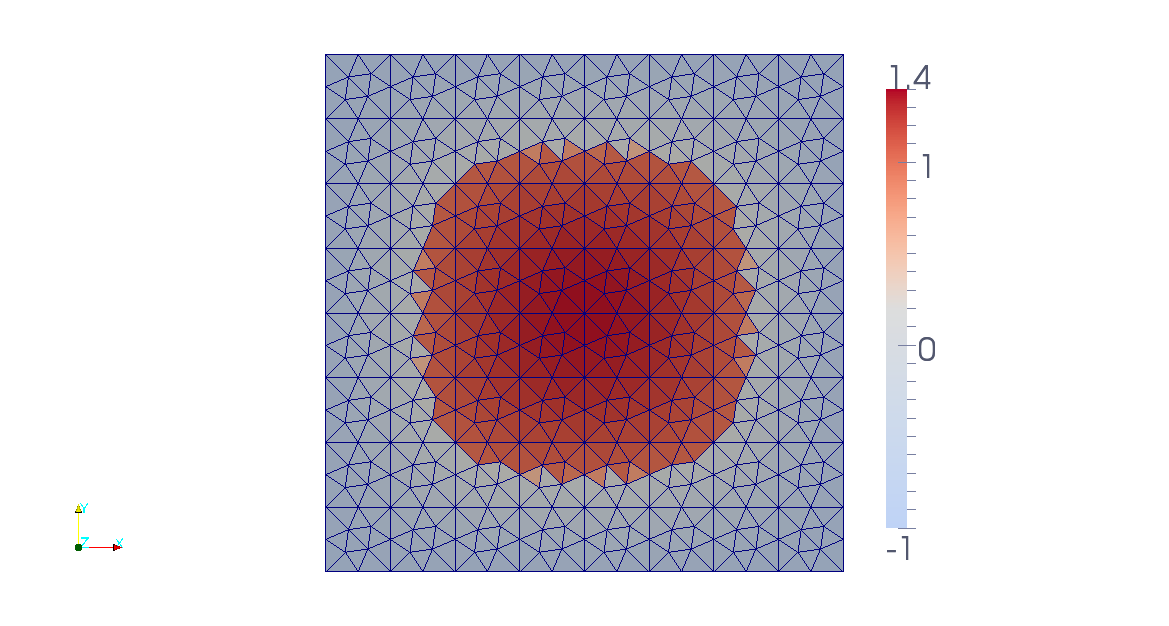
\includegraphics[trim=11.cm 2.cm 11.cm 2.cm,clip=true,scale=0.18]{figNum/tri_T50.png}}
  \subfigure[Kershaw]{\label{2D_T50_ker}
  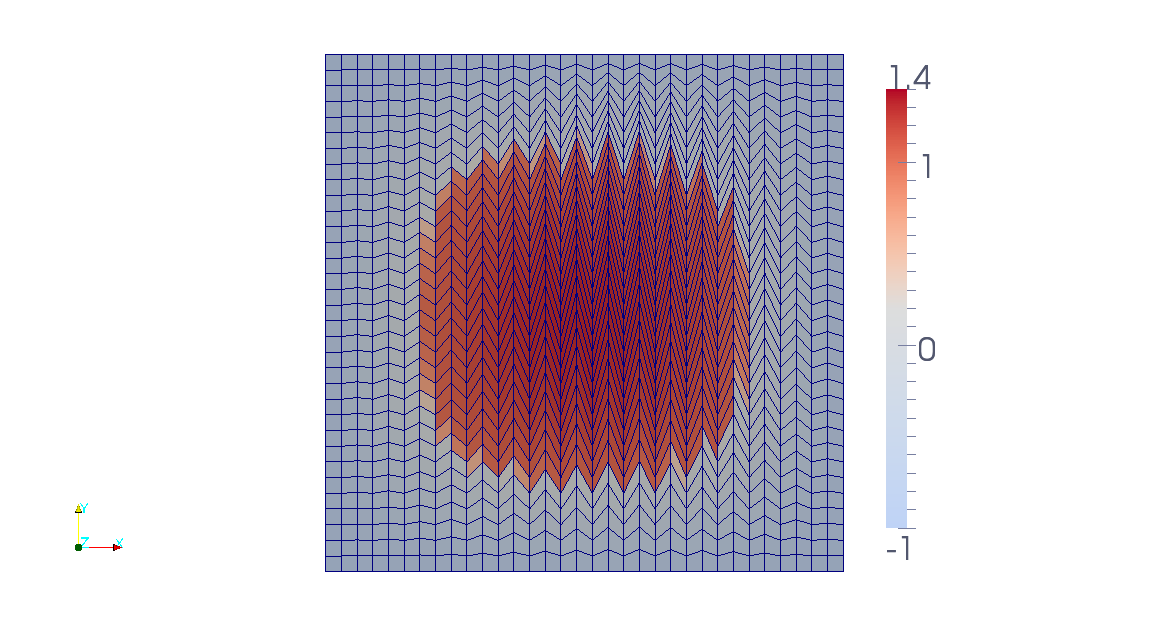
\includegraphics[trim=11.cm 2.cm. 7.cm 2.cm,clip=true,scale=0.18]{figNum/ker_T50.png}}
\caption{Discrete solution $u$ on all grids at $t=0.050$.\label{fig:2D_T50}
}
\end{figure}

\begin{figure}[ht]
%trim=left bottom right top
 \centering
  \subfigure[Cartesian]{\label{2D_T75_cart}
  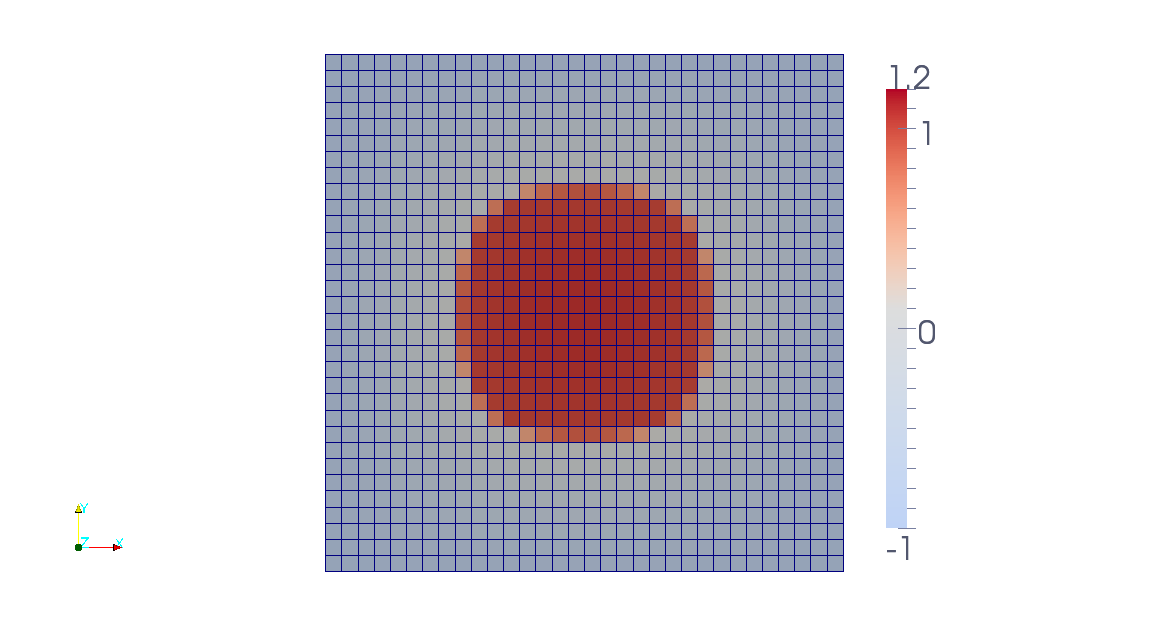
\includegraphics[trim=11.cm 2.cm 11.cm 2.cm,clip=true,scale=0.18]{figNum/cart_T75.png}}
  \subfigure[Perturbed Cartesian]{\label{2D_T75_rand}
  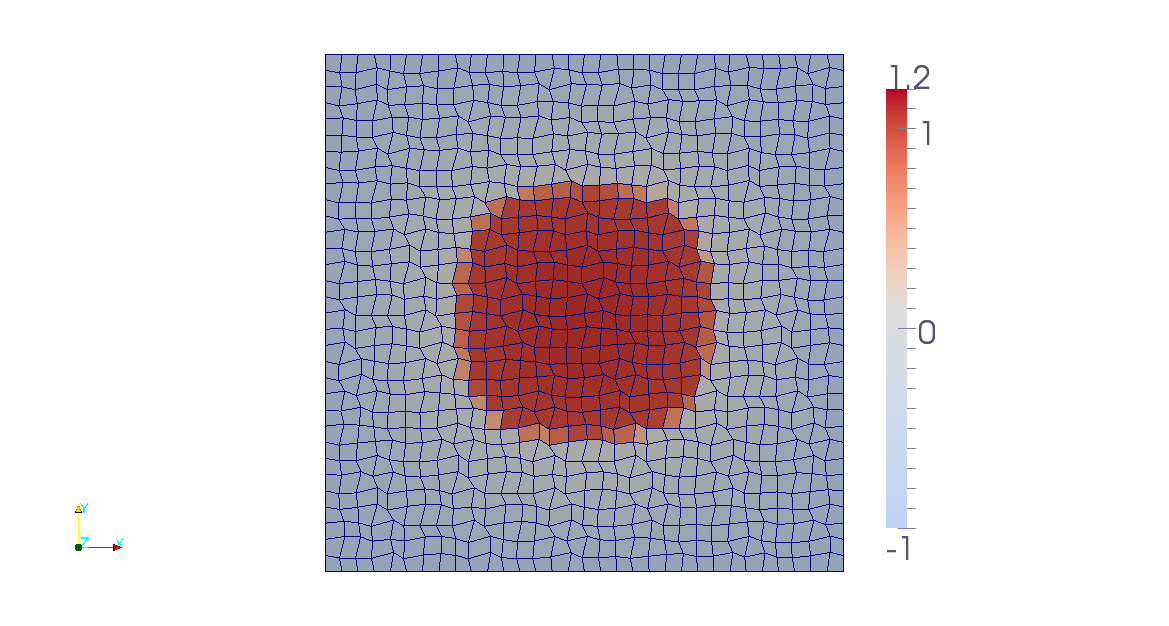
\includegraphics[trim=11.cm 2.cm 11.cm 2.cm,clip=true,scale=0.18]{figNum/rand_T75.png}}\\
  \subfigure[Triangular]{\label{f2D_T75_tria}
  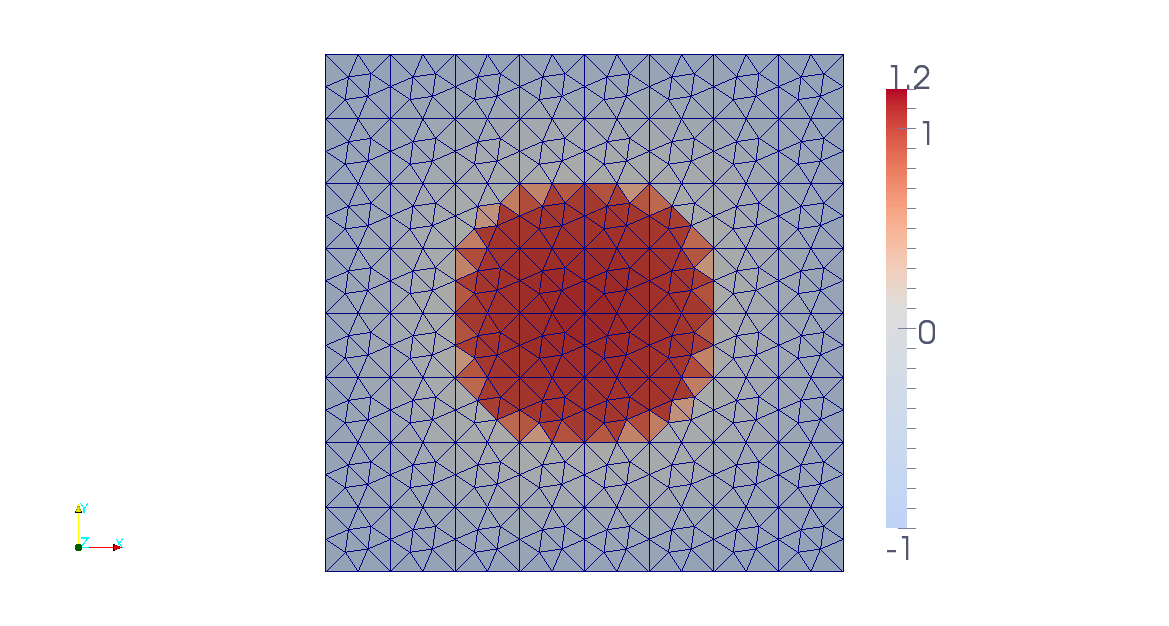
\includegraphics[trim=11.cm 2.cm 11.cm 2.cm,clip=true,scale=0.18]{figNum/tri_T75.png}}
  \subfigure[Kershaw]{\label{2D_T75_ker}
  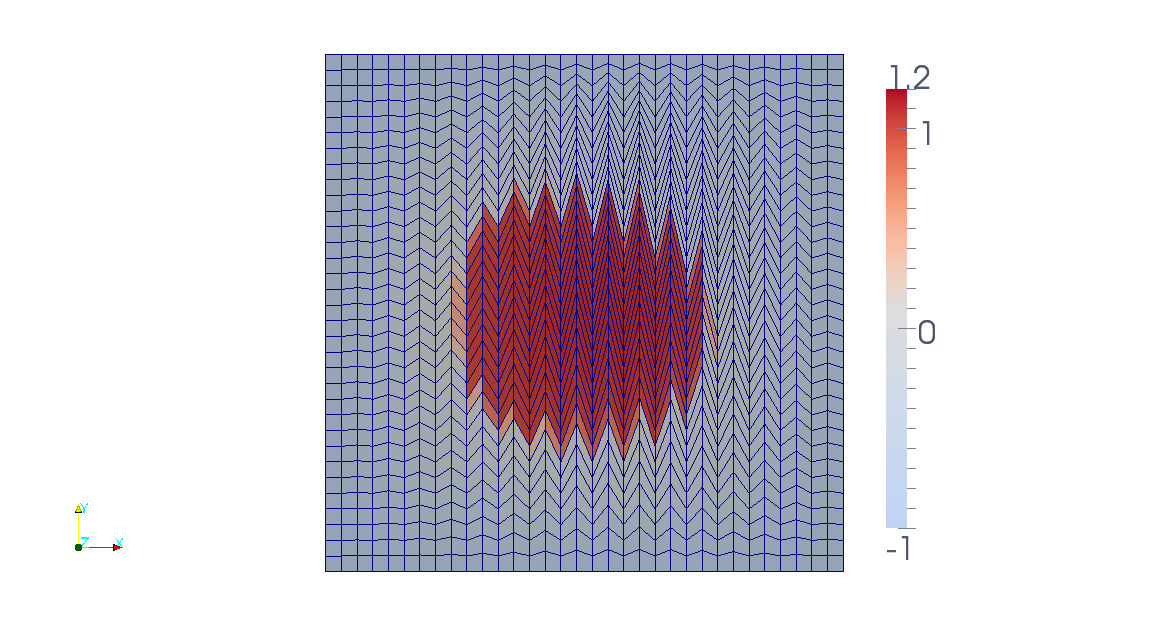
\includegraphics[trim=11.cm 2.cm. 7.cm 2.cm,clip=true,scale=0.18]{figNum/ker_T75.png}}
\caption{Discrete solution $u$ on all grids at $t=0.075$.
\label{fig:2D_T75}
}
\end{figure}


\begin{figure}[ht]
%trim=left bottom right top
 \centering
  \subfigure[Cartesian]{\label{2D_T100_cart}
  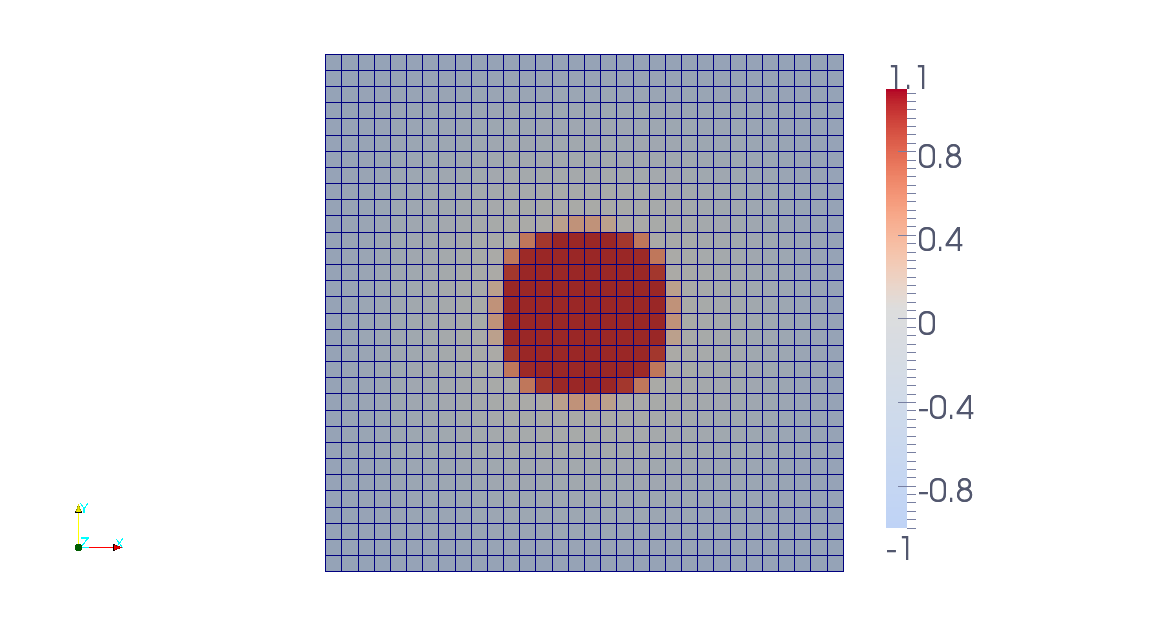
\includegraphics[trim=11.cm 2.cm 11.cm 2.cm,clip=true,scale=0.18]{figNum/cart_T100.png}}
  \subfigure[Perturbed Cartesian]{\label{2D_T100_rand}
  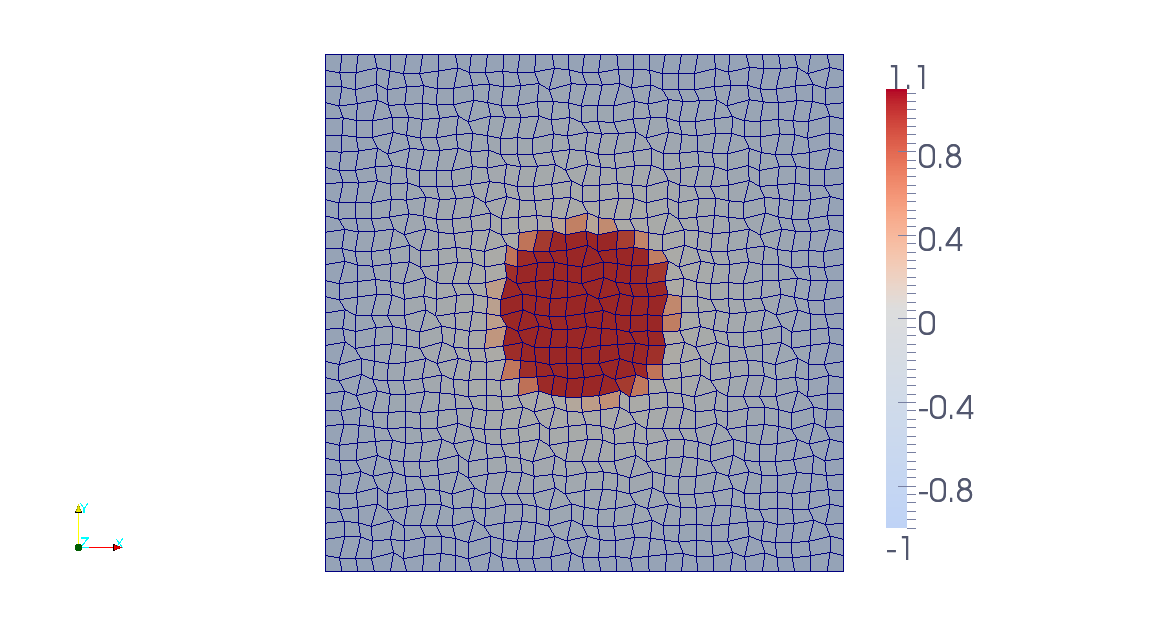
\includegraphics[trim=11.cm 2.cm 11.cm 2.cm,clip=true,scale=0.18]{figNum/rand_T100.png}}\\
  \subfigure[Triangular]{\label{f2D_T100_tria}
  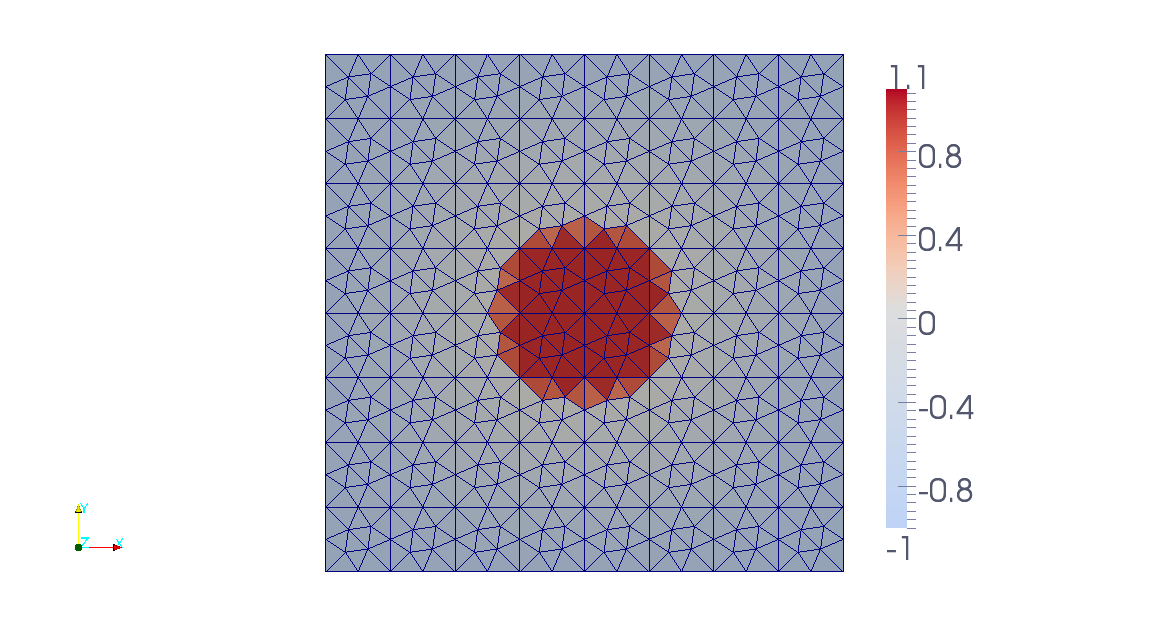
\includegraphics[trim=11.cm 2.cm 11.cm 2.cm,clip=true,scale=0.18]{figNum/tri_T100.png}}
  \subfigure[Kershaw]{\label{2D_T100_ker}
  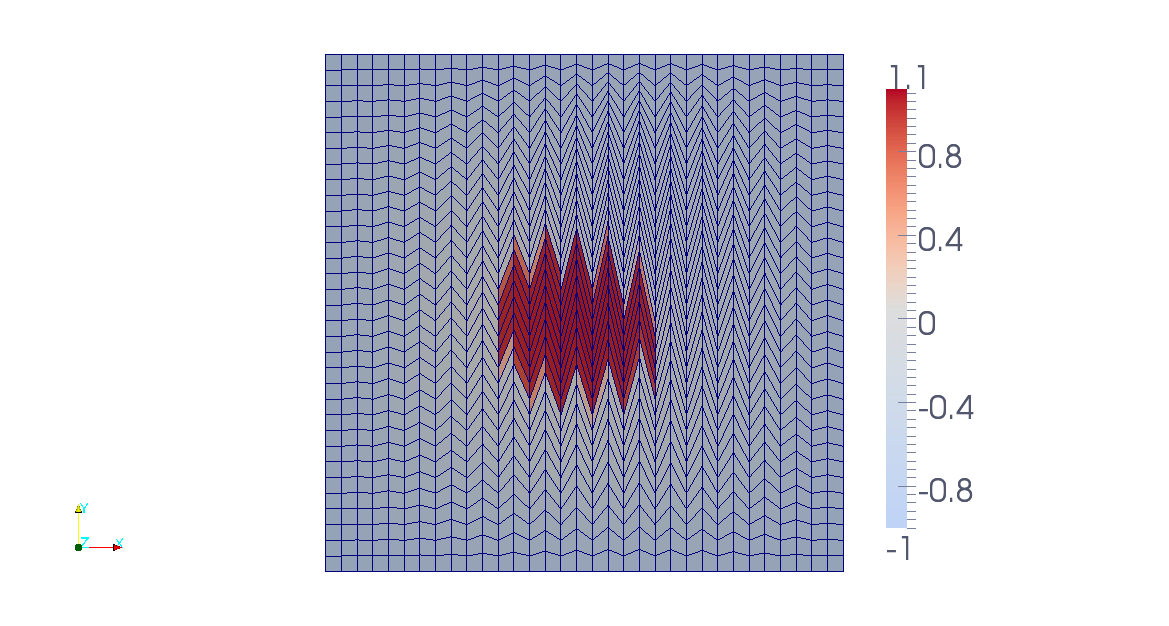
\includegraphics[trim=11.cm 2.cm. 7.cm 2.cm,clip=true,scale=0.18]{figNum/ker_T100.png}}
\caption{Discrete solution $u$ on all grids at $t=0.1$.
\label{fig:2D_T100}
}
\end{figure}


% \input gagsns.tex 
\backmatter%%%%%%%%%%%%%%%%%%%%%%%%%%%%%%%%%%%%%%%%%%%%%%%%%%%%%%%
%\addcontentsline{toc}{chapter}{Bibliography}
\bibliographystyle{abbrv}
\bibliography{gabib}

\newpage

\pagestyle{empty}

\section*{Abbreviations} 
\addcontentsline{toc}{chapter}{Abbreviations}

\begin{tabular}{ll}
BC & Boundary Condition\\
CeVeFE & Cell--Vertex--Face/Edge \\
CDO & Compatible Discrete Operator\\
DDFV & Discrete Duality Finite Volume\\
DGGD & Discontinuous Galerkin gradient discretization\\
GD & Gradient Discretisation\\
GDM & Gradient Discretisation Method\\
GS & Gradient Scheme\\
HFV & Hybrid Finite Volume\\
hMFD & hybrid Mimetic Finite Difference\\
HMM & Hybrid Mimetic Mixed\\
LLE & Local Linearly Exact\\
MFD & Mimetic Finite Difference\\
MFE & Mixed Finite Element\\
MPFA & Multi-Point Flux Approximation\\
MPFA-O & Multi-Point Flux Approximation O-scheme\\
nMFD & nodal Mimetic Finite Difference\\
PDE & Partial Differential Equation \\
SIPG & Symmetric Interior Penalty Galerkin \\
SUSHI & Scheme Using Stabilization and  Hybrid Interfaces \\
TPFA & Two-Point Flux Approximation \\
TPFA-CG & Two-Point Flux Approximation for Cartesian Grids \\
VAG & Vertex Approximate Gradient \\
\end{tabular}

\printindex[abb]
\addcontentsline{toc}{chapter}{Notations}
\printindex
\addcontentsline{toc}{chapter}{Index}

\ifthenelse{\boolean{ToPrint}}{ \end{twocolumn} }

\end{document}

